\documentclass[twoside]{book}

% Packages required by doxygen
\usepackage{fixltx2e}
\usepackage{calc}
\usepackage{doxygen}
\usepackage{graphicx}
\usepackage[utf8]{inputenc}
\usepackage{makeidx}
\usepackage{multicol}
\usepackage{multirow}
\PassOptionsToPackage{warn}{textcomp}
\usepackage{textcomp}
\usepackage[nointegrals]{wasysym}
\usepackage[table]{xcolor}

% Font selection
\usepackage[T1]{fontenc}
\usepackage{mathptmx}
\usepackage[scaled=.90]{helvet}
\usepackage{courier}
\usepackage{amssymb}
\usepackage{sectsty}
\renewcommand{\familydefault}{\sfdefault}
\allsectionsfont{%
  \fontseries{bc}\selectfont%
  \color{darkgray}%
}
\renewcommand{\DoxyLabelFont}{%
  \fontseries{bc}\selectfont%
  \color{darkgray}%
}
\newcommand{\+}{\discretionary{\mbox{\scriptsize$\hookleftarrow$}}{}{}}

% Page & text layout
\usepackage{geometry}
\geometry{%
  a4paper,%
  top=2.5cm,%
  bottom=2.5cm,%
  left=2.5cm,%
  right=2.5cm%
}
\tolerance=750
\hfuzz=15pt
\hbadness=750
\setlength{\emergencystretch}{15pt}
\setlength{\parindent}{0cm}
\setlength{\parskip}{0.2cm}
\makeatletter
\renewcommand{\paragraph}{%
  \@startsection{paragraph}{4}{0ex}{-1.0ex}{1.0ex}{%
    \normalfont\normalsize\bfseries\SS@parafont%
  }%
}
\renewcommand{\subparagraph}{%
  \@startsection{subparagraph}{5}{0ex}{-1.0ex}{1.0ex}{%
    \normalfont\normalsize\bfseries\SS@subparafont%
  }%
}
\makeatother

% Headers & footers
\usepackage{fancyhdr}
\pagestyle{fancyplain}
\fancyhead[LE]{\fancyplain{}{\bfseries\thepage}}
\fancyhead[CE]{\fancyplain{}{}}
\fancyhead[RE]{\fancyplain{}{\bfseries\leftmark}}
\fancyhead[LO]{\fancyplain{}{\bfseries\rightmark}}
\fancyhead[CO]{\fancyplain{}{}}
\fancyhead[RO]{\fancyplain{}{\bfseries\thepage}}
\fancyfoot[LE]{\fancyplain{}{}}
\fancyfoot[CE]{\fancyplain{}{}}
\fancyfoot[RE]{\fancyplain{}{\bfseries\scriptsize Generated on Tue Sep 16 2014 20\+:24\+:54 for ractiphom by Doxygen }}
\fancyfoot[LO]{\fancyplain{}{\bfseries\scriptsize Generated on Tue Sep 16 2014 20\+:24\+:54 for ractiphom by Doxygen }}
\fancyfoot[CO]{\fancyplain{}{}}
\fancyfoot[RO]{\fancyplain{}{}}
\renewcommand{\footrulewidth}{0.4pt}
\renewcommand{\chaptermark}[1]{%
  \markboth{#1}{}%
}
\renewcommand{\sectionmark}[1]{%
  \markright{\thesection\ #1}%
}

% Indices & bibliography
\usepackage{natbib}
\usepackage[titles]{tocloft}
\setcounter{tocdepth}{3}
\setcounter{secnumdepth}{5}
\makeindex

% Hyperlinks (required, but should be loaded last)
\usepackage{ifpdf}
\ifpdf
  \usepackage[pdftex,pagebackref=true]{hyperref}
\else
  \usepackage[ps2pdf,pagebackref=true]{hyperref}
\fi
\hypersetup{%
  colorlinks=true,%
  linkcolor=blue,%
  citecolor=blue,%
  unicode%
}

% Custom commands
\newcommand{\clearemptydoublepage}{%
  \newpage{\pagestyle{empty}\cleardoublepage}%
}


%===== C O N T E N T S =====

\begin{document}

% Titlepage & ToC
\hypersetup{pageanchor=false,
             bookmarks=true,
             bookmarksnumbered=true,
             pdfencoding=unicode
            }
\pagenumbering{roman}
\begin{titlepage}
\vspace*{7cm}
\begin{center}%
{\Large ractiphom }\\
\vspace*{1cm}
{\large Generated by Doxygen 1.8.8}\\
\vspace*{0.5cm}
{\small Tue Sep 16 2014 20:24:54}\\
\end{center}
\end{titlepage}
\clearemptydoublepage
\tableofcontents
\clearemptydoublepage
\pagenumbering{arabic}
\hypersetup{pageanchor=true}

%--- Begin generated contents ---
\chapter{Deprecated List}
\label{deprecated}
\hypertarget{deprecated}{}

\begin{DoxyRefList}
\item[\label{deprecated__deprecated000001}%
\hypertarget{deprecated__deprecated000001}{}%
Member \hyperlink{cmdline1_8c_a78a0cd581698415a62f68214603b1a30}{cmdline\+\_\+parser2} (int argc, char $\ast$$\ast$argv, struct \hyperlink{structgengetopt__args__info}{gengetopt\+\_\+args\+\_\+info} $\ast$args\+\_\+info, int override, int initialize, int check\+\_\+required)]use \hyperlink{cmdline_8c_ac7bb5d76f3f56d1c0b3b531f11ac6f07}{cmdline\+\_\+parser\+\_\+ext()} instead 

use \hyperlink{cmdline_8c_ac7bb5d76f3f56d1c0b3b531f11ac6f07}{cmdline\+\_\+parser\+\_\+ext()} instead 
\end{DoxyRefList}
\chapter{Namespace Index}
\section{Namespace List}
Here is a list of all namespaces with brief descriptions\+:\begin{DoxyCompactList}
\item\contentsline{section}{\hyperlink{namespace_centroid}{Centroid} }{\pageref{namespace_centroid}}{}
\item\contentsline{section}{\hyperlink{namespace_c_o_n_t_r_a_l_i_g_n}{C\+O\+N\+T\+R\+A\+L\+I\+G\+N} }{\pageref{namespace_c_o_n_t_r_a_l_i_g_n}}{}
\item\contentsline{section}{\hyperlink{namespace_h_c_l_u_s_t}{H\+C\+L\+U\+S\+T} }{\pageref{namespace_h_c_l_u_s_t}}{}
\item\contentsline{section}{\hyperlink{namespace_m_e_a}{M\+E\+A} }{\pageref{namespace_m_e_a}}{}
\item\contentsline{section}{\hyperlink{namespace_p_r_o_b_c_o_n_s}{P\+R\+O\+B\+C\+O\+N\+S} }{\pageref{namespace_p_r_o_b_c_o_n_s}}{}
\item\contentsline{section}{\hyperlink{namespace_rule}{Rule} }{\pageref{namespace_rule}}{}
\item\contentsline{section}{\hyperlink{namespaceu_shuffle}{u\+Shuffle} }{\pageref{namespaceu_shuffle}}{}
\item\contentsline{section}{\hyperlink{namespace_vienna}{Vienna} }{\pageref{namespace_vienna}}{}
\end{DoxyCompactList}

\chapter{Hierarchical Index}
\section{Class Hierarchy}
This inheritance list is sorted roughly, but not completely, alphabetically\+:\begin{DoxyCompactList}
\item \contentsline{section}{Aln}{\pageref{class_aln}}{}
\item \contentsline{section}{fa\+\_\+parser\+:\+:append\+\_\+seq}{\pageref{structfa__parser_1_1append__seq}}{}
\item \contentsline{section}{Average\+B\+P}{\pageref{struct_average_b_p}}{}
\item \contentsline{section}{B\+P\+Table\+Tmpl$<$ T $>$}{\pageref{class_b_p_table_tmpl}}{}
\item \contentsline{section}{B\+P\+Table\+Tmpl$<$ float $>$}{\pageref{class_b_p_table_tmpl}}{}
\item \contentsline{section}{M\+E\+A\+:\+:Cell$<$ V $>$}{\pageref{struct_m_e_a_1_1_cell}}{}
\item \contentsline{section}{Centroid\+:\+:Cell$<$ V $>$}{\pageref{struct_centroid_1_1_cell}}{}
\item \contentsline{section}{C\+F\+Wrapper}{\pageref{class_c_f_wrapper}}{}
\item \contentsline{section}{cmdline\+\_\+parser\+\_\+params}{\pageref{structcmdline__parser__params}}{}
\item \contentsline{section}{cmp\+\_\+by\+\_\+mcc}{\pageref{structcmp__by__mcc}}{}
\item \contentsline{section}{cmp\+\_\+by\+\_\+size}{\pageref{structcmp__by__size}}{}
\item \contentsline{section}{connection}{\pageref{structconnection}}{}
\item \contentsline{section}{C\+O\+N\+T\+R\+Afold$<$ T $>$}{\pageref{class_c_o_n_t_r_afold}}{}
\item \contentsline{section}{C\+O\+N\+T\+R\+Afold$<$ float $>$}{\pageref{class_c_o_n_t_r_afold}}{}
\item \contentsline{section}{C\+O\+N\+T\+R\+Afold\+M$<$ T $>$}{\pageref{class_c_o_n_t_r_afold_m}}{}
\item \contentsline{section}{C\+O\+N\+T\+R\+Afold\+M$<$ float $>$}{\pageref{class_c_o_n_t_r_afold_m}}{}
\item \contentsline{section}{C\+O\+N\+T\+R\+A\+L\+I\+G\+N\+:\+:C\+O\+N\+T\+R\+Align$<$ T $>$}{\pageref{class_c_o_n_t_r_a_l_i_g_n_1_1_c_o_n_t_r_align}}{}
\item \contentsline{section}{Count\+B\+P$<$ L $>$}{\pageref{struct_count_b_p}}{}
\item \contentsline{section}{C\+Y\+K\+Table$<$ T $>$}{\pageref{class_c_y_k_table}}{}
\item \contentsline{section}{C\+Y\+K\+Table$<$ float $>$}{\pageref{class_c_y_k_table}}{}
\item \contentsline{section}{C\+Y\+K\+Table$<$ uint $>$}{\pageref{class_c_y_k_table}}{}
\item \contentsline{section}{C\+Y\+K\+Table$<$ V $>$}{\pageref{class_c_y_k_table}}{}
\item \contentsline{section}{aln\+\_\+parser\+:\+:definition$<$ Scanner\+T $>$}{\pageref{structaln__parser_1_1definition}}{}
\item \contentsline{section}{fa\+\_\+parser\+:\+:definition$<$ Scanner\+T $>$}{\pageref{structfa__parser_1_1definition}}{}
\item \contentsline{section}{H\+C\+L\+U\+S\+T\+:\+:Diana$<$ D\+Matrix $>$}{\pageref{class_h_c_l_u_s_t_1_1_diana}}{}
\item \contentsline{section}{Die}{\pageref{class_die}}{}
\item \contentsline{section}{Div}{\pageref{struct_div}}{}
\item \contentsline{section}{Duplex\+Engine$<$ Real\+T $>$}{\pageref{class_duplex_engine}}{}
\item \contentsline{section}{Folding\+Engine$<$ S\+E\+Q $>$\+:\+:Encode\+B\+P}{\pageref{struct_folding_engine_1_1_encode_b_p}}{}
\item \contentsline{section}{Centroid\+:\+:Estimator$<$ T $>$}{\pageref{struct_centroid_1_1_estimator}}{}
\item \contentsline{section}{Fasta}{\pageref{class_fasta}}{}
\item \contentsline{section}{P\+R\+O\+B\+C\+O\+N\+S\+:\+:File\+Buffer}{\pageref{class_p_r_o_b_c_o_n_s_1_1_file_buffer}}{}
\item \contentsline{section}{Folding\+Engine$<$ S\+E\+Q $>$}{\pageref{class_folding_engine}}{}
\begin{DoxyCompactList}
\item \contentsline{section}{Mixture\+Model$<$ S\+E\+Q $>$}{\pageref{class_mixture_model}}{}
\item \contentsline{section}{Pfold\+Model$<$ S\+E\+Q $>$}{\pageref{class_pfold_model}}{}
\end{DoxyCompactList}
\item \contentsline{section}{Folding\+Engine$<$ Aln $>$}{\pageref{class_folding_engine}}{}
\begin{DoxyCompactList}
\item \contentsline{section}{Averaged\+Model}{\pageref{class_averaged_model}}{}
\item \contentsline{section}{C\+O\+N\+T\+R\+Afold\+Multi\+Model}{\pageref{class_c_o_n_t_r_afold_multi_model}}{}
\end{DoxyCompactList}
\item \contentsline{section}{Folding\+Engine$<$ std\+:\+:string $>$}{\pageref{class_folding_engine}}{}
\begin{DoxyCompactList}
\item \contentsline{section}{Aux\+Model}{\pageref{class_aux_model}}{}
\item \contentsline{section}{C\+O\+N\+T\+R\+Afold\+Model}{\pageref{class_c_o_n_t_r_afold_model}}{}
\end{DoxyCompactList}
\item \contentsline{section}{Folding\+Engine$<$ T\+H $>$}{\pageref{class_folding_engine}}{}
\begin{DoxyCompactList}
\item \contentsline{section}{C\+O\+N\+T\+R\+Afold\+Hom\+Model}{\pageref{class_c_o_n_t_r_afold_hom_model}}{}
\end{DoxyCompactList}
\item \contentsline{section}{gengetopt\+\_\+args\+\_\+info}{\pageref{structgengetopt__args__info}}{}
\item grammar\begin{DoxyCompactList}
\item \contentsline{section}{aln\+\_\+parser}{\pageref{structaln__parser}}{}
\item \contentsline{section}{fa\+\_\+parser}{\pageref{structfa__parser}}{}
\item \contentsline{section}{fa\+\_\+parser}{\pageref{structfa__parser}}{}
\end{DoxyCompactList}
\item \contentsline{section}{hentry}{\pageref{structhentry}}{}
\item \contentsline{section}{Ignore\+Alone\+Pair$<$ Table $>$}{\pageref{struct_ignore_alone_pair}}{}
\item \contentsline{section}{C\+O\+N\+T\+R\+Afold$<$ T $>$\+:\+:Impl}{\pageref{struct_c_o_n_t_r_afold_1_1_impl}}{}
\item \contentsline{section}{P\+R\+O\+B\+C\+O\+N\+S\+:\+:Probcons\+:\+:Impl}{\pageref{struct_p_r_o_b_c_o_n_s_1_1_probcons_1_1_impl}}{}
\item \contentsline{section}{C\+O\+N\+T\+R\+A\+L\+I\+G\+N\+:\+:C\+O\+N\+T\+R\+Align$<$ T $>$\+:\+:Impl}{\pageref{struct_c_o_n_t_r_a_l_i_g_n_1_1_c_o_n_t_r_align_1_1_impl}}{}
\item \contentsline{section}{C\+O\+N\+T\+R\+Afold\+M$<$ T $>$\+:\+:Impl}{\pageref{struct_c_o_n_t_r_afold_m_1_1_impl}}{}
\item \contentsline{section}{Inference\+Engine$<$ Real\+T $>$}{\pageref{class_inference_engine}}{}
\item \contentsline{section}{C\+O\+N\+T\+R\+A\+L\+I\+G\+N\+:\+:Inference\+Engine$<$ Real\+T $>$}{\pageref{class_c_o_n_t_r_a_l_i_g_n_1_1_inference_engine}}{}
\item \contentsline{section}{Inference\+Engine$<$ T $>$}{\pageref{class_inference_engine}}{}
\item \contentsline{section}{C\+O\+N\+T\+R\+A\+L\+I\+G\+N\+:\+:Inference\+Engine$<$ T $>$}{\pageref{class_c_o_n_t_r_a_l_i_g_n_1_1_inference_engine}}{}
\item \contentsline{section}{I\+P}{\pageref{class_i_p}}{}
\item \contentsline{section}{I\+U\+P\+A\+Csymbol}{\pageref{class_i_u_p_a_csymbol}}{}
\item logic\+\_\+error\begin{DoxyCompactList}
\item \contentsline{section}{aln\+\_\+parser\+:\+:format\+\_\+error}{\pageref{classaln__parser_1_1format__error}}{}
\end{DoxyCompactList}
\item \contentsline{section}{loop}{\pageref{structloop}}{}
\item \contentsline{section}{Mul\+Add}{\pageref{struct_mul_add}}{}
\item \contentsline{section}{P\+R\+O\+B\+C\+O\+N\+S\+:\+:Multi\+Sequence}{\pageref{class_p_r_o_b_c_o_n_s_1_1_multi_sequence}}{}
\item \contentsline{section}{C\+O\+N\+T\+R\+A\+L\+I\+G\+N\+:\+:Multi\+Sequence}{\pageref{class_c_o_n_t_r_a_l_i_g_n_1_1_multi_sequence}}{}
\item pair\begin{DoxyCompactList}
\item \contentsline{section}{Alignment}{\pageref{class_alignment}}{}
\item \contentsline{section}{T\+H}{\pageref{class_t_h}}{}
\end{DoxyCompactList}
\item \contentsline{section}{C\+O\+N\+T\+R\+A\+L\+I\+G\+N\+:\+:Parameter\+Group}{\pageref{struct_c_o_n_t_r_a_l_i_g_n_1_1_parameter_group}}{}
\item \contentsline{section}{Parameter\+Group}{\pageref{struct_parameter_group}}{}
\item \contentsline{section}{C\+O\+N\+T\+R\+A\+L\+I\+G\+N\+:\+:Parameter\+Manager$<$ Real\+T $>$}{\pageref{class_c_o_n_t_r_a_l_i_g_n_1_1_parameter_manager}}{}
\item \contentsline{section}{Parameter\+Manager$<$ Real\+T $>$}{\pageref{class_parameter_manager}}{}
\item \contentsline{section}{C\+O\+N\+T\+R\+A\+L\+I\+G\+N\+:\+:Parameter\+Manager$<$ T $>$}{\pageref{class_c_o_n_t_r_a_l_i_g_n_1_1_parameter_manager}}{}
\item \contentsline{section}{Parameter\+Manager$<$ T $>$}{\pageref{class_parameter_manager}}{}
\item \contentsline{section}{P\+R\+O\+B\+C\+O\+N\+S\+:\+:Probabilistic\+Model}{\pageref{class_p_r_o_b_c_o_n_s_1_1_probabilistic_model}}{}
\item \contentsline{section}{P\+R\+O\+B\+C\+O\+N\+S\+:\+:Probcons}{\pageref{class_p_r_o_b_c_o_n_s_1_1_probcons}}{}
\item \contentsline{section}{C\+O\+N\+T\+R\+A\+L\+I\+G\+N\+:\+:Progressive$<$ Real\+T $>$}{\pageref{class_c_o_n_t_r_a_l_i_g_n_1_1_progressive}}{}
\item \contentsline{section}{aln\+\_\+parser\+:\+:push\+\_\+seq}{\pageref{structaln__parser_1_1push__seq}}{}
\item \contentsline{section}{Ract\+I\+P}{\pageref{class_ract_i_p}}{}
\item \contentsline{section}{radloop}{\pageref{structradloop}}{}
\item \contentsline{section}{region}{\pageref{structregion}}{}
\item \contentsline{section}{aln\+\_\+parser\+:\+:reset\+\_\+index}{\pageref{structaln__parser_1_1reset__index}}{}
\item \contentsline{section}{Result}{\pageref{struct_result}}{}
\item \contentsline{section}{R\+N\+Aduplex\+Hommodel}{\pageref{class_r_n_aduplex_hommodel}}{}
\item \contentsline{section}{Roulette$<$ T, Real\+T $>$}{\pageref{class_roulette}}{}
\item \contentsline{section}{C\+O\+N\+T\+R\+A\+L\+I\+G\+N\+:\+:Sequence}{\pageref{class_c_o_n_t_r_a_l_i_g_n_1_1_sequence}}{}
\item \contentsline{section}{P\+R\+O\+B\+C\+O\+N\+S\+:\+:Sequence}{\pageref{class_p_r_o_b_c_o_n_s_1_1_sequence}}{}
\item \contentsline{section}{P\+R\+O\+B\+C\+O\+N\+S\+:\+:Sparse\+Matrix}{\pageref{class_p_r_o_b_c_o_n_s_1_1_sparse_matrix}}{}
\item \contentsline{section}{C\+O\+N\+T\+R\+A\+L\+I\+G\+N\+:\+:Sparse\+Matrix$<$ T $>$}{\pageref{class_c_o_n_t_r_a_l_i_g_n_1_1_sparse_matrix}}{}
\item \contentsline{section}{C\+O\+N\+T\+R\+A\+L\+I\+G\+N\+:\+:Sparse\+Matrix\+Entry$<$ T $>$}{\pageref{struct_c_o_n_t_r_a_l_i_g_n_1_1_sparse_matrix_entry}}{}
\item \contentsline{section}{C\+O\+N\+T\+R\+A\+L\+I\+G\+N\+:\+:S\+Struct}{\pageref{class_c_o_n_t_r_a_l_i_g_n_1_1_s_struct}}{}
\item \contentsline{section}{S\+Struct}{\pageref{class_s_struct}}{}
\item \contentsline{section}{tetra\+\_\+loops}{\pageref{structtetra__loops}}{}
\item \contentsline{section}{Centroid\+:\+:Trace\+Back$<$ D\+P\+Table $>$}{\pageref{struct_centroid_1_1_trace_back}}{}
\item \contentsline{section}{M\+E\+A\+:\+:Trace\+Back$<$ D\+P\+Table $>$}{\pageref{struct_m_e_a_1_1_trace_back}}{}
\item \contentsline{section}{C\+O\+N\+T\+R\+A\+L\+I\+G\+N\+:\+:Tree$<$ Real\+T $>$}{\pageref{class_c_o_n_t_r_a_l_i_g_n_1_1_tree}}{}
\item \contentsline{section}{C\+O\+N\+T\+R\+A\+L\+I\+G\+N\+:\+:Tree$<$ Real\+T $>$\+:\+:Tree\+Node}{\pageref{struct_c_o_n_t_r_a_l_i_g_n_1_1_tree_1_1_tree_node}}{}
\item \contentsline{section}{C\+O\+N\+T\+R\+A\+L\+I\+G\+N\+:\+:triple$<$ T1, T2, T3 $>$}{\pageref{struct_c_o_n_t_r_a_l_i_g_n_1_1triple}}{}
\item \contentsline{section}{triple$<$ T1, T2, T3 $>$}{\pageref{structtriple}}{}
\item \contentsline{section}{M\+E\+A\+:\+:Updater$<$ B\+P\+Table, D\+P\+Table $>$}{\pageref{struct_m_e_a_1_1_updater}}{}
\item \contentsline{section}{Updater$<$ V $>$}{\pageref{struct_updater}}{}
\item \contentsline{section}{Centroid\+:\+:Updater$<$ B\+P\+Table, D\+P\+Table $>$}{\pageref{struct_centroid_1_1_updater}}{}
\item vector\begin{DoxyCompactList}
\item \contentsline{section}{P\+R\+O\+B\+C\+O\+N\+S\+:\+:Safe\+Vector$<$ T\+Y\+P\+E $>$}{\pageref{class_p_r_o_b_c_o_n_s_1_1_safe_vector}}{}
\item \contentsline{section}{P\+R\+O\+B\+C\+O\+N\+S\+:\+:Safe\+Vector$<$ char $>$}{\pageref{class_p_r_o_b_c_o_n_s_1_1_safe_vector}}{}
\item \contentsline{section}{P\+R\+O\+B\+C\+O\+N\+S\+:\+:Safe\+Vector$<$ int $>$}{\pageref{class_p_r_o_b_c_o_n_s_1_1_safe_vector}}{}
\item \contentsline{section}{P\+R\+O\+B\+C\+O\+N\+S\+:\+:Safe\+Vector$<$ P\+I\+F $>$}{\pageref{class_p_r_o_b_c_o_n_s_1_1_safe_vector}}{}
\item \contentsline{section}{P\+R\+O\+B\+C\+O\+N\+S\+:\+:Safe\+Vector$<$ P\+R\+O\+B\+C\+O\+N\+S\+:\+:Safe\+Vector$<$ P\+I\+F $>$\+:\+:iterator $>$}{\pageref{class_p_r_o_b_c_o_n_s_1_1_safe_vector}}{}
\item \contentsline{section}{P\+R\+O\+B\+C\+O\+N\+S\+:\+:Safe\+Vector$<$ P\+R\+O\+B\+C\+O\+N\+S\+:\+:Sequence $\ast$ $>$}{\pageref{class_p_r_o_b_c_o_n_s_1_1_safe_vector}}{}
\end{DoxyCompactList}
\item \contentsline{section}{vertex}{\pageref{structvertex}}{}
\item \contentsline{section}{aln\+\_\+parser\+:\+:W\+A}{\pageref{structaln__parser_1_1_w_a}}{}
\end{DoxyCompactList}

\chapter{Class Index}
\section{Class List}
Here are the classes, structs, unions and interfaces with brief descriptions\+:\begin{DoxyCompactList}
\item\contentsline{section}{\hyperlink{class_alignment}{Alignment} }{\pageref{class_alignment}}{}
\item\contentsline{section}{\hyperlink{class_aln}{Aln} }{\pageref{class_aln}}{}
\item\contentsline{section}{\hyperlink{structaln__parser}{aln\+\_\+parser} }{\pageref{structaln__parser}}{}
\item\contentsline{section}{\hyperlink{structfa__parser_1_1append__seq}{fa\+\_\+parser\+::append\+\_\+seq} }{\pageref{structfa__parser_1_1append__seq}}{}
\item\contentsline{section}{\hyperlink{class_aux_model}{Aux\+Model} }{\pageref{class_aux_model}}{}
\item\contentsline{section}{\hyperlink{struct_average_b_p}{Average\+B\+P} }{\pageref{struct_average_b_p}}{}
\item\contentsline{section}{\hyperlink{class_averaged_model}{Averaged\+Model} }{\pageref{class_averaged_model}}{}
\item\contentsline{section}{\hyperlink{class_b_p_table_tmpl}{B\+P\+Table\+Tmpl$<$ T $>$} }{\pageref{class_b_p_table_tmpl}}{}
\item\contentsline{section}{\hyperlink{struct_m_e_a_1_1_cell}{M\+E\+A\+::\+Cell$<$ V $>$} }{\pageref{struct_m_e_a_1_1_cell}}{}
\item\contentsline{section}{\hyperlink{struct_centroid_1_1_cell}{Centroid\+::\+Cell$<$ V $>$} }{\pageref{struct_centroid_1_1_cell}}{}
\item\contentsline{section}{\hyperlink{class_c_f_wrapper}{C\+F\+Wrapper} }{\pageref{class_c_f_wrapper}}{}
\item\contentsline{section}{\hyperlink{structcmdline__parser__params}{cmdline\+\_\+parser\+\_\+params} \\*The additional parameters to pass to parser functions }{\pageref{structcmdline__parser__params}}{}
\item\contentsline{section}{\hyperlink{structcmp__by__mcc}{cmp\+\_\+by\+\_\+mcc} }{\pageref{structcmp__by__mcc}}{}
\item\contentsline{section}{\hyperlink{structcmp__by__size}{cmp\+\_\+by\+\_\+size} }{\pageref{structcmp__by__size}}{}
\item\contentsline{section}{\hyperlink{structconnection}{connection} }{\pageref{structconnection}}{}
\item\contentsline{section}{\hyperlink{class_c_o_n_t_r_afold}{C\+O\+N\+T\+R\+Afold$<$ T $>$} }{\pageref{class_c_o_n_t_r_afold}}{}
\item\contentsline{section}{\hyperlink{class_c_o_n_t_r_afold_hom_model}{C\+O\+N\+T\+R\+Afold\+Hom\+Model} }{\pageref{class_c_o_n_t_r_afold_hom_model}}{}
\item\contentsline{section}{\hyperlink{class_c_o_n_t_r_afold_m}{C\+O\+N\+T\+R\+Afold\+M$<$ T $>$} }{\pageref{class_c_o_n_t_r_afold_m}}{}
\item\contentsline{section}{\hyperlink{class_c_o_n_t_r_afold_model}{C\+O\+N\+T\+R\+Afold\+Model} }{\pageref{class_c_o_n_t_r_afold_model}}{}
\item\contentsline{section}{\hyperlink{class_c_o_n_t_r_afold_multi_model}{C\+O\+N\+T\+R\+Afold\+Multi\+Model} }{\pageref{class_c_o_n_t_r_afold_multi_model}}{}
\item\contentsline{section}{\hyperlink{class_c_o_n_t_r_a_l_i_g_n_1_1_c_o_n_t_r_align}{C\+O\+N\+T\+R\+A\+L\+I\+G\+N\+::\+C\+O\+N\+T\+R\+Align$<$ T $>$} }{\pageref{class_c_o_n_t_r_a_l_i_g_n_1_1_c_o_n_t_r_align}}{}
\item\contentsline{section}{\hyperlink{struct_count_b_p}{Count\+B\+P$<$ L $>$} }{\pageref{struct_count_b_p}}{}
\item\contentsline{section}{\hyperlink{class_c_y_k_table}{C\+Y\+K\+Table$<$ T $>$} \\*A templete class of C\+Y\+K tables used for Cocke-\/\+Younger-\/\+Kasami (C\+Y\+K) algorithm }{\pageref{class_c_y_k_table}}{}
\item\contentsline{section}{\hyperlink{structaln__parser_1_1definition}{aln\+\_\+parser\+::definition$<$ Scanner\+T $>$} }{\pageref{structaln__parser_1_1definition}}{}
\item\contentsline{section}{\hyperlink{structfa__parser_1_1definition}{fa\+\_\+parser\+::definition$<$ Scanner\+T $>$} }{\pageref{structfa__parser_1_1definition}}{}
\item\contentsline{section}{\hyperlink{class_h_c_l_u_s_t_1_1_diana}{H\+C\+L\+U\+S\+T\+::\+Diana$<$ D\+Matrix $>$} }{\pageref{class_h_c_l_u_s_t_1_1_diana}}{}
\item\contentsline{section}{\hyperlink{class_die}{Die} }{\pageref{class_die}}{}
\item\contentsline{section}{\hyperlink{struct_div}{Div} }{\pageref{struct_div}}{}
\item\contentsline{section}{\hyperlink{class_duplex_engine}{Duplex\+Engine$<$ Real\+T $>$} }{\pageref{class_duplex_engine}}{}
\item\contentsline{section}{\hyperlink{struct_folding_engine_1_1_encode_b_p}{Folding\+Engine$<$ S\+E\+Q $>$\+::\+Encode\+B\+P} }{\pageref{struct_folding_engine_1_1_encode_b_p}}{}
\item\contentsline{section}{\hyperlink{struct_centroid_1_1_estimator}{Centroid\+::\+Estimator$<$ T $>$} }{\pageref{struct_centroid_1_1_estimator}}{}
\item\contentsline{section}{\hyperlink{structfa__parser}{fa\+\_\+parser} }{\pageref{structfa__parser}}{}
\item\contentsline{section}{\hyperlink{class_fasta}{Fasta} }{\pageref{class_fasta}}{}
\item\contentsline{section}{\hyperlink{class_p_r_o_b_c_o_n_s_1_1_file_buffer}{P\+R\+O\+B\+C\+O\+N\+S\+::\+File\+Buffer} }{\pageref{class_p_r_o_b_c_o_n_s_1_1_file_buffer}}{}
\item\contentsline{section}{\hyperlink{class_folding_engine}{Folding\+Engine$<$ S\+E\+Q $>$} }{\pageref{class_folding_engine}}{}
\item\contentsline{section}{\hyperlink{classaln__parser_1_1format__error}{aln\+\_\+parser\+::format\+\_\+error} }{\pageref{classaln__parser_1_1format__error}}{}
\item\contentsline{section}{\hyperlink{structgengetopt__args__info}{gengetopt\+\_\+args\+\_\+info} \\*Where the command line options are stored }{\pageref{structgengetopt__args__info}}{}
\item\contentsline{section}{\hyperlink{structhentry}{hentry} }{\pageref{structhentry}}{}
\item\contentsline{section}{\hyperlink{struct_ignore_alone_pair}{Ignore\+Alone\+Pair$<$ Table $>$} }{\pageref{struct_ignore_alone_pair}}{}
\item\contentsline{section}{\hyperlink{struct_c_o_n_t_r_afold_1_1_impl}{C\+O\+N\+T\+R\+Afold$<$ T $>$\+::\+Impl} }{\pageref{struct_c_o_n_t_r_afold_1_1_impl}}{}
\item\contentsline{section}{\hyperlink{struct_p_r_o_b_c_o_n_s_1_1_probcons_1_1_impl}{P\+R\+O\+B\+C\+O\+N\+S\+::\+Probcons\+::\+Impl} }{\pageref{struct_p_r_o_b_c_o_n_s_1_1_probcons_1_1_impl}}{}
\item\contentsline{section}{\hyperlink{struct_c_o_n_t_r_a_l_i_g_n_1_1_c_o_n_t_r_align_1_1_impl}{C\+O\+N\+T\+R\+A\+L\+I\+G\+N\+::\+C\+O\+N\+T\+R\+Align$<$ T $>$\+::\+Impl} }{\pageref{struct_c_o_n_t_r_a_l_i_g_n_1_1_c_o_n_t_r_align_1_1_impl}}{}
\item\contentsline{section}{\hyperlink{struct_c_o_n_t_r_afold_m_1_1_impl}{C\+O\+N\+T\+R\+Afold\+M$<$ T $>$\+::\+Impl} }{\pageref{struct_c_o_n_t_r_afold_m_1_1_impl}}{}
\item\contentsline{section}{\hyperlink{class_inference_engine}{Inference\+Engine$<$ Real\+T $>$} }{\pageref{class_inference_engine}}{}
\item\contentsline{section}{\hyperlink{class_c_o_n_t_r_a_l_i_g_n_1_1_inference_engine}{C\+O\+N\+T\+R\+A\+L\+I\+G\+N\+::\+Inference\+Engine$<$ Real\+T $>$} }{\pageref{class_c_o_n_t_r_a_l_i_g_n_1_1_inference_engine}}{}
\item\contentsline{section}{\hyperlink{class_i_p}{I\+P} }{\pageref{class_i_p}}{}
\item\contentsline{section}{\hyperlink{class_i_u_p_a_csymbol}{I\+U\+P\+A\+Csymbol} }{\pageref{class_i_u_p_a_csymbol}}{}
\item\contentsline{section}{\hyperlink{structloop}{loop} }{\pageref{structloop}}{}
\item\contentsline{section}{\hyperlink{class_mixture_model}{Mixture\+Model$<$ S\+E\+Q $>$} }{\pageref{class_mixture_model}}{}
\item\contentsline{section}{\hyperlink{struct_mul_add}{Mul\+Add} }{\pageref{struct_mul_add}}{}
\item\contentsline{section}{\hyperlink{class_p_r_o_b_c_o_n_s_1_1_multi_sequence}{P\+R\+O\+B\+C\+O\+N\+S\+::\+Multi\+Sequence} }{\pageref{class_p_r_o_b_c_o_n_s_1_1_multi_sequence}}{}
\item\contentsline{section}{\hyperlink{class_c_o_n_t_r_a_l_i_g_n_1_1_multi_sequence}{C\+O\+N\+T\+R\+A\+L\+I\+G\+N\+::\+Multi\+Sequence} }{\pageref{class_c_o_n_t_r_a_l_i_g_n_1_1_multi_sequence}}{}
\item\contentsline{section}{\hyperlink{struct_c_o_n_t_r_a_l_i_g_n_1_1_parameter_group}{C\+O\+N\+T\+R\+A\+L\+I\+G\+N\+::\+Parameter\+Group} }{\pageref{struct_c_o_n_t_r_a_l_i_g_n_1_1_parameter_group}}{}
\item\contentsline{section}{\hyperlink{struct_parameter_group}{Parameter\+Group} }{\pageref{struct_parameter_group}}{}
\item\contentsline{section}{\hyperlink{class_c_o_n_t_r_a_l_i_g_n_1_1_parameter_manager}{C\+O\+N\+T\+R\+A\+L\+I\+G\+N\+::\+Parameter\+Manager$<$ Real\+T $>$} }{\pageref{class_c_o_n_t_r_a_l_i_g_n_1_1_parameter_manager}}{}
\item\contentsline{section}{\hyperlink{class_parameter_manager}{Parameter\+Manager$<$ Real\+T $>$} }{\pageref{class_parameter_manager}}{}
\item\contentsline{section}{\hyperlink{class_pfold_model}{Pfold\+Model$<$ S\+E\+Q $>$} }{\pageref{class_pfold_model}}{}
\item\contentsline{section}{\hyperlink{class_p_r_o_b_c_o_n_s_1_1_probabilistic_model}{P\+R\+O\+B\+C\+O\+N\+S\+::\+Probabilistic\+Model} }{\pageref{class_p_r_o_b_c_o_n_s_1_1_probabilistic_model}}{}
\item\contentsline{section}{\hyperlink{class_p_r_o_b_c_o_n_s_1_1_probcons}{P\+R\+O\+B\+C\+O\+N\+S\+::\+Probcons} }{\pageref{class_p_r_o_b_c_o_n_s_1_1_probcons}}{}
\item\contentsline{section}{\hyperlink{class_c_o_n_t_r_a_l_i_g_n_1_1_progressive}{C\+O\+N\+T\+R\+A\+L\+I\+G\+N\+::\+Progressive$<$ Real\+T $>$} }{\pageref{class_c_o_n_t_r_a_l_i_g_n_1_1_progressive}}{}
\item\contentsline{section}{\hyperlink{structaln__parser_1_1push__seq}{aln\+\_\+parser\+::push\+\_\+seq} }{\pageref{structaln__parser_1_1push__seq}}{}
\item\contentsline{section}{\hyperlink{class_ract_i_p}{Ract\+I\+P} }{\pageref{class_ract_i_p}}{}
\item\contentsline{section}{\hyperlink{structradloop}{radloop} }{\pageref{structradloop}}{}
\item\contentsline{section}{\hyperlink{structregion}{region} }{\pageref{structregion}}{}
\item\contentsline{section}{\hyperlink{structaln__parser_1_1reset__index}{aln\+\_\+parser\+::reset\+\_\+index} }{\pageref{structaln__parser_1_1reset__index}}{}
\item\contentsline{section}{\hyperlink{struct_result}{Result} }{\pageref{struct_result}}{}
\item\contentsline{section}{\hyperlink{class_r_n_aduplex_hommodel}{R\+N\+Aduplex\+Hommodel} }{\pageref{class_r_n_aduplex_hommodel}}{}
\item\contentsline{section}{\hyperlink{class_roulette}{Roulette$<$ T, Real\+T $>$} }{\pageref{class_roulette}}{}
\item\contentsline{section}{\hyperlink{class_p_r_o_b_c_o_n_s_1_1_safe_vector}{P\+R\+O\+B\+C\+O\+N\+S\+::\+Safe\+Vector$<$ T\+Y\+P\+E $>$} }{\pageref{class_p_r_o_b_c_o_n_s_1_1_safe_vector}}{}
\item\contentsline{section}{\hyperlink{class_c_o_n_t_r_a_l_i_g_n_1_1_sequence}{C\+O\+N\+T\+R\+A\+L\+I\+G\+N\+::\+Sequence} }{\pageref{class_c_o_n_t_r_a_l_i_g_n_1_1_sequence}}{}
\item\contentsline{section}{\hyperlink{class_p_r_o_b_c_o_n_s_1_1_sequence}{P\+R\+O\+B\+C\+O\+N\+S\+::\+Sequence} }{\pageref{class_p_r_o_b_c_o_n_s_1_1_sequence}}{}
\item\contentsline{section}{\hyperlink{class_p_r_o_b_c_o_n_s_1_1_sparse_matrix}{P\+R\+O\+B\+C\+O\+N\+S\+::\+Sparse\+Matrix} }{\pageref{class_p_r_o_b_c_o_n_s_1_1_sparse_matrix}}{}
\item\contentsline{section}{\hyperlink{class_c_o_n_t_r_a_l_i_g_n_1_1_sparse_matrix}{C\+O\+N\+T\+R\+A\+L\+I\+G\+N\+::\+Sparse\+Matrix$<$ T $>$} }{\pageref{class_c_o_n_t_r_a_l_i_g_n_1_1_sparse_matrix}}{}
\item\contentsline{section}{\hyperlink{struct_c_o_n_t_r_a_l_i_g_n_1_1_sparse_matrix_entry}{C\+O\+N\+T\+R\+A\+L\+I\+G\+N\+::\+Sparse\+Matrix\+Entry$<$ T $>$} }{\pageref{struct_c_o_n_t_r_a_l_i_g_n_1_1_sparse_matrix_entry}}{}
\item\contentsline{section}{\hyperlink{class_c_o_n_t_r_a_l_i_g_n_1_1_s_struct}{C\+O\+N\+T\+R\+A\+L\+I\+G\+N\+::\+S\+Struct} }{\pageref{class_c_o_n_t_r_a_l_i_g_n_1_1_s_struct}}{}
\item\contentsline{section}{\hyperlink{class_s_struct}{S\+Struct} }{\pageref{class_s_struct}}{}
\item\contentsline{section}{\hyperlink{structtetra__loops}{tetra\+\_\+loops} }{\pageref{structtetra__loops}}{}
\item\contentsline{section}{\hyperlink{class_t_h}{T\+H} }{\pageref{class_t_h}}{}
\item\contentsline{section}{\hyperlink{struct_centroid_1_1_trace_back}{Centroid\+::\+Trace\+Back$<$ D\+P\+Table $>$} }{\pageref{struct_centroid_1_1_trace_back}}{}
\item\contentsline{section}{\hyperlink{struct_m_e_a_1_1_trace_back}{M\+E\+A\+::\+Trace\+Back$<$ D\+P\+Table $>$} }{\pageref{struct_m_e_a_1_1_trace_back}}{}
\item\contentsline{section}{\hyperlink{class_c_o_n_t_r_a_l_i_g_n_1_1_tree}{C\+O\+N\+T\+R\+A\+L\+I\+G\+N\+::\+Tree$<$ Real\+T $>$} }{\pageref{class_c_o_n_t_r_a_l_i_g_n_1_1_tree}}{}
\item\contentsline{section}{\hyperlink{struct_c_o_n_t_r_a_l_i_g_n_1_1_tree_1_1_tree_node}{C\+O\+N\+T\+R\+A\+L\+I\+G\+N\+::\+Tree$<$ Real\+T $>$\+::\+Tree\+Node} }{\pageref{struct_c_o_n_t_r_a_l_i_g_n_1_1_tree_1_1_tree_node}}{}
\item\contentsline{section}{\hyperlink{struct_c_o_n_t_r_a_l_i_g_n_1_1triple}{C\+O\+N\+T\+R\+A\+L\+I\+G\+N\+::triple$<$ T1, T2, T3 $>$} }{\pageref{struct_c_o_n_t_r_a_l_i_g_n_1_1triple}}{}
\item\contentsline{section}{\hyperlink{structtriple}{triple$<$ T1, T2, T3 $>$} }{\pageref{structtriple}}{}
\item\contentsline{section}{\hyperlink{struct_m_e_a_1_1_updater}{M\+E\+A\+::\+Updater$<$ B\+P\+Table, D\+P\+Table $>$} }{\pageref{struct_m_e_a_1_1_updater}}{}
\item\contentsline{section}{\hyperlink{struct_updater}{Updater$<$ V $>$} }{\pageref{struct_updater}}{}
\item\contentsline{section}{\hyperlink{struct_centroid_1_1_updater}{Centroid\+::\+Updater$<$ B\+P\+Table, D\+P\+Table $>$} }{\pageref{struct_centroid_1_1_updater}}{}
\item\contentsline{section}{\hyperlink{structvertex}{vertex} }{\pageref{structvertex}}{}
\item\contentsline{section}{\hyperlink{structaln__parser_1_1_w_a}{aln\+\_\+parser\+::\+W\+A} }{\pageref{structaln__parser_1_1_w_a}}{}
\end{DoxyCompactList}

\chapter{File Index}
\section{File List}
Here is a list of all files with brief descriptions\+:\begin{DoxyCompactList}
\item\contentsline{section}{src/\hyperlink{alignment_8h}{alignment.\+h} }{\pageref{alignment_8h}}{}
\item\contentsline{section}{src/\hyperlink{boltzmann__param_8c}{boltzmann\+\_\+param.\+c} }{\pageref{boltzmann__param_8c}}{}
\item\contentsline{section}{src/\hyperlink{boltzmann__param_8h}{boltzmann\+\_\+param.\+h} }{\pageref{boltzmann__param_8h}}{}
\item\contentsline{section}{src/\hyperlink{cmdline_8c}{cmdline.\+c} }{\pageref{cmdline_8c}}{}
\item\contentsline{section}{src/\hyperlink{cmdline_8h}{cmdline.\+h} \\*The header file for the command line option parser generated by G\+N\+U Gengetopt version 2.\+22.\+6 \href{http://www.gnu.org/software/gengetopt}{\tt http\+://www.\+gnu.\+org/software/gengetopt}. D\+O N\+O\+T modify this file, since it can be overwritten }{\pageref{cmdline_8h}}{}
\item\contentsline{section}{src/\hyperlink{cmdline1_8c}{cmdline1.\+c} }{\pageref{cmdline1_8c}}{}
\item\contentsline{section}{src/\hyperlink{cmdline1_8h}{cmdline1.\+h} \\*The header file for the command line option parser generated by G\+N\+U Gengetopt version 2.\+22.\+6 \href{http://www.gnu.org/software/gengetopt}{\tt http\+://www.\+gnu.\+org/software/gengetopt}. D\+O N\+O\+T modify this file, since it can be overwritten }{\pageref{cmdline1_8h}}{}
\item\contentsline{section}{src/\hyperlink{duplex_hom_8cpp}{duplex\+Hom.\+cpp} }{\pageref{duplex_hom_8cpp}}{}
\item\contentsline{section}{src/\hyperlink{duplex_hom_8h}{duplex\+Hom.\+h} }{\pageref{duplex_hom_8h}}{}
\item\contentsline{section}{src/\hyperlink{fa_8cpp}{fa.\+cpp} }{\pageref{fa_8cpp}}{}
\item\contentsline{section}{src/\hyperlink{fa_8h}{fa.\+h} }{\pageref{fa_8h}}{}
\item\contentsline{section}{src/\hyperlink{ip_8cpp}{ip.\+cpp} }{\pageref{ip_8cpp}}{}
\item\contentsline{section}{src/\hyperlink{ip_8h}{ip.\+h} }{\pageref{ip_8h}}{}
\item\contentsline{section}{src/\hyperlink{linktest_8cpp}{linktest.\+cpp} }{\pageref{linktest_8cpp}}{}
\item\contentsline{section}{src/\hyperlink{notespace_8cpp}{notespace.\+cpp} }{\pageref{notespace_8cpp}}{}
\item\contentsline{section}{src/\hyperlink{pf__duplex_8c}{pf\+\_\+duplex.\+c} }{\pageref{pf__duplex_8c}}{}
\item\contentsline{section}{src/\hyperlink{pf__duplex_8h}{pf\+\_\+duplex.\+h} }{\pageref{pf__duplex_8h}}{}
\item\contentsline{section}{src/\hyperlink{ractip_8cpp}{ractip.\+cpp} }{\pageref{ractip_8cpp}}{}
\item\contentsline{section}{src/\hyperlink{ractip__hom_8cpp}{ractip\+\_\+hom.\+cpp} }{\pageref{ractip__hom_8cpp}}{}
\item\contentsline{section}{src/\hyperlink{ushuffle_8c}{ushuffle.\+c} }{\pageref{ushuffle_8c}}{}
\item\contentsline{section}{src/\hyperlink{ushuffle_8h}{ushuffle.\+h} }{\pageref{ushuffle_8h}}{}
\item\contentsline{section}{src/\hyperlink{vvf_8h}{vvf.\+h} }{\pageref{vvf_8h}}{}
\item\contentsline{section}{src/centroidalifold/\hyperlink{aln_8cpp}{aln.\+cpp} }{\pageref{aln_8cpp}}{}
\item\contentsline{section}{src/centroidalifold/\hyperlink{aln_8h}{aln.\+h} }{\pageref{aln_8h}}{}
\item\contentsline{section}{src/centroidalifold/\hyperlink{bp_8cpp}{bp.\+cpp} }{\pageref{bp_8cpp}}{}
\item\contentsline{section}{src/centroidalifold/\hyperlink{bp_8h}{bp.\+h} }{\pageref{bp_8h}}{}
\item\contentsline{section}{src/centroidalifold/\hyperlink{capi_8cpp}{capi.\+cpp} }{\pageref{capi_8cpp}}{}
\item\contentsline{section}{src/centroidalifold/\hyperlink{capi_8h}{capi.\+h} }{\pageref{capi_8h}}{}
\item\contentsline{section}{src/centroidalifold/\hyperlink{centroid_8cpp}{centroid.\+cpp} }{\pageref{centroid_8cpp}}{}
\item\contentsline{section}{src/centroidalifold/\hyperlink{centroid_8h}{centroid.\+h} }{\pageref{centroid_8h}}{}
\item\contentsline{section}{src/centroidalifold/\hyperlink{centroid__alifold_8cpp}{centroid\+\_\+alifold.\+cpp} }{\pageref{centroid__alifold_8cpp}}{}
\item\contentsline{section}{src/centroidalifold/\hyperlink{centroid__fold_8cpp}{centroid\+\_\+fold.\+cpp} }{\pageref{centroid__fold_8cpp}}{}
\item\contentsline{section}{src/centroidalifold/\hyperlink{centroid__homfold_8cpp}{centroid\+\_\+homfold.\+cpp} }{\pageref{centroid__homfold_8cpp}}{}
\item\contentsline{section}{src/centroidalifold/\hyperlink{cyktable_8h}{cyktable.\+h} }{\pageref{cyktable_8h}}{}
\item\contentsline{section}{src/centroidalifold/\hyperlink{diana_8cpp}{diana.\+cpp} }{\pageref{diana_8cpp}}{}
\item\contentsline{section}{src/centroidalifold/\hyperlink{diana_8h}{diana.\+h} }{\pageref{diana_8h}}{}
\item\contentsline{section}{src/centroidalifold/\hyperlink{centroidalifold_2fa_8cpp}{fa.\+cpp} }{\pageref{centroidalifold_2fa_8cpp}}{}
\item\contentsline{section}{src/centroidalifold/\hyperlink{centroidalifold_2fa_8h}{fa.\+h} }{\pageref{centroidalifold_2fa_8h}}{}
\item\contentsline{section}{src/centroidalifold/\hyperlink{folding__engine_8cpp}{folding\+\_\+engine.\+cpp} }{\pageref{folding__engine_8cpp}}{}
\item\contentsline{section}{src/centroidalifold/\hyperlink{folding__engine_8h}{folding\+\_\+engine.\+h} }{\pageref{folding__engine_8h}}{}
\item\contentsline{section}{src/centroidalifold/\hyperlink{iupac_8cpp}{iupac.\+cpp} }{\pageref{iupac_8cpp}}{}
\item\contentsline{section}{src/centroidalifold/\hyperlink{iupac_8h}{iupac.\+h} }{\pageref{iupac_8h}}{}
\item\contentsline{section}{src/centroidalifold/\hyperlink{log__prob_8cpp}{log\+\_\+prob.\+cpp} }{\pageref{log__prob_8cpp}}{}
\item\contentsline{section}{src/centroidalifold/\hyperlink{mea_8cpp}{mea.\+cpp} }{\pageref{mea_8cpp}}{}
\item\contentsline{section}{src/centroidalifold/\hyperlink{mea_8h}{mea.\+h} }{\pageref{mea_8h}}{}
\item\contentsline{section}{src/centroidalifold/\hyperlink{naview_8c}{naview.\+c} }{\pageref{naview_8c}}{}
\item\contentsline{section}{src/centroidalifold/\hyperlink{ps__plot_8cpp}{ps\+\_\+plot.\+cpp} }{\pageref{ps__plot_8cpp}}{}
\item\contentsline{section}{src/centroidalifold/\hyperlink{ps__plot_8h}{ps\+\_\+plot.\+h} }{\pageref{ps__plot_8h}}{}
\item\contentsline{section}{src/centroidalifold/\hyperlink{rule_8h}{rule.\+h} }{\pageref{rule_8h}}{}
\item\contentsline{section}{src/centroidalifold/\hyperlink{test_8c}{test.\+c} }{\pageref{test_8c}}{}
\item\contentsline{section}{src/centroidalifold/\hyperlink{util_8h}{util.\+h} }{\pageref{util_8h}}{}
\item\contentsline{section}{src/centroidalifold/contrafold/\hyperlink{centroidalifold_2contrafold_2_config_8hpp}{Config.\+hpp} }{\pageref{centroidalifold_2contrafold_2_config_8hpp}}{}
\item\contentsline{section}{src/centroidalifold/contrafold/\hyperlink{contrafold_2contrafold_8h}{contrafold.\+h} }{\pageref{contrafold_2contrafold_8h}}{}
\item\contentsline{section}{src/centroidalifold/contrafold/\hyperlink{centroidalifold_2contrafold_2_defaults_8ipp}{Defaults.\+ipp} }{\pageref{centroidalifold_2contrafold_2_defaults_8ipp}}{}
\item\contentsline{section}{src/centroidalifold/contrafold/\hyperlink{errortest_8cpp}{errortest.\+cpp} }{\pageref{errortest_8cpp}}{}
\item\contentsline{section}{src/centroidalifold/contrafold/\hyperlink{errortest_8hpp}{errortest.\+hpp} }{\pageref{errortest_8hpp}}{}
\item\contentsline{section}{src/centroidalifold/contrafold/\hyperlink{centroidalifold_2contrafold_2_inference_engine_8hpp}{Inference\+Engine.\+hpp} }{\pageref{centroidalifold_2contrafold_2_inference_engine_8hpp}}{}
\item\contentsline{section}{src/centroidalifold/contrafold/\hyperlink{centroidalifold_2contrafold_2_inference_engine_8ipp}{Inference\+Engine.\+ipp} }{\pageref{centroidalifold_2contrafold_2_inference_engine_8ipp}}{}
\item\contentsline{section}{src/centroidalifold/contrafold/\hyperlink{centroidalifold_2contrafold_2_log_space_8hpp}{Log\+Space.\+hpp} }{\pageref{centroidalifold_2contrafold_2_log_space_8hpp}}{}
\item\contentsline{section}{src/centroidalifold/contrafold/\hyperlink{centroidalifold_2contrafold_2_parameter_manager_8hpp}{Parameter\+Manager.\+hpp} }{\pageref{centroidalifold_2contrafold_2_parameter_manager_8hpp}}{}
\item\contentsline{section}{src/centroidalifold/contrafold/\hyperlink{centroidalifold_2contrafold_2_parameter_manager_8ipp}{Parameter\+Manager.\+ipp} }{\pageref{centroidalifold_2contrafold_2_parameter_manager_8ipp}}{}
\item\contentsline{section}{src/centroidalifold/contrafold/\hyperlink{centroidalifold_2contrafold_2rand_8h}{rand.\+h} }{\pageref{centroidalifold_2contrafold_2rand_8h}}{}
\item\contentsline{section}{src/centroidalifold/contrafold/\hyperlink{centroidalifold_2contrafold_2_s_struct_8cpp}{S\+Struct.\+cpp} }{\pageref{centroidalifold_2contrafold_2_s_struct_8cpp}}{}
\item\contentsline{section}{src/centroidalifold/contrafold/\hyperlink{centroidalifold_2contrafold_2_s_struct_8hpp}{S\+Struct.\+hpp} }{\pageref{centroidalifold_2contrafold_2_s_struct_8hpp}}{}
\item\contentsline{section}{src/centroidalifold/contrafold/\hyperlink{centroidalifold_2contrafold_2_utilities_8cpp}{Utilities.\+cpp} }{\pageref{centroidalifold_2contrafold_2_utilities_8cpp}}{}
\item\contentsline{section}{src/centroidalifold/contrafold/\hyperlink{centroidalifold_2contrafold_2_utilities_8hpp}{Utilities.\+hpp} }{\pageref{centroidalifold_2contrafold_2_utilities_8hpp}}{}
\item\contentsline{section}{src/centroidalifold/contrafold/\hyperlink{centroidalifold_2contrafold_2_utilities_8ipp}{Utilities.\+ipp} }{\pageref{centroidalifold_2contrafold_2_utilities_8ipp}}{}
\item\contentsline{section}{src/centroidalifold/contrafold/\hyperlink{contrafold_2wrapper_8cpp}{wrapper.\+cpp} }{\pageref{contrafold_2wrapper_8cpp}}{}
\item\contentsline{section}{src/centroidalifold/contralign/\hyperlink{centroidalifold_2contralign_2_config_8hpp}{Config.\+hpp} }{\pageref{centroidalifold_2contralign_2_config_8hpp}}{}
\item\contentsline{section}{src/centroidalifold/contralign/\hyperlink{_contralign_8cpp}{Contralign.\+cpp} }{\pageref{_contralign_8cpp}}{}
\item\contentsline{section}{src/centroidalifold/contralign/\hyperlink{contralign_8h}{contralign.\+h} }{\pageref{contralign_8h}}{}
\item\contentsline{section}{src/centroidalifold/contralign/\hyperlink{centroidalifold_2contralign_2_defaults_8ipp}{Defaults.\+ipp} }{\pageref{centroidalifold_2contralign_2_defaults_8ipp}}{}
\item\contentsline{section}{src/centroidalifold/contralign/\hyperlink{centroidalifold_2contralign_2_inference_engine_8hpp}{Inference\+Engine.\+hpp} }{\pageref{centroidalifold_2contralign_2_inference_engine_8hpp}}{}
\item\contentsline{section}{src/centroidalifold/contralign/\hyperlink{centroidalifold_2contralign_2_inference_engine_8ipp}{Inference\+Engine.\+ipp} }{\pageref{centroidalifold_2contralign_2_inference_engine_8ipp}}{}
\item\contentsline{section}{src/centroidalifold/contralign/\hyperlink{centroidalifold_2contralign_2_log_space_8hpp}{Log\+Space.\+hpp} }{\pageref{centroidalifold_2contralign_2_log_space_8hpp}}{}
\item\contentsline{section}{src/centroidalifold/contralign/\hyperlink{_multi_sequence_8cpp}{Multi\+Sequence.\+cpp} }{\pageref{_multi_sequence_8cpp}}{}
\item\contentsline{section}{src/centroidalifold/contralign/\hyperlink{_multi_sequence_8hpp}{Multi\+Sequence.\+hpp} }{\pageref{_multi_sequence_8hpp}}{}
\item\contentsline{section}{src/centroidalifold/contralign/\hyperlink{centroidalifold_2contralign_2_parameter_manager_8hpp}{Parameter\+Manager.\+hpp} }{\pageref{centroidalifold_2contralign_2_parameter_manager_8hpp}}{}
\item\contentsline{section}{src/centroidalifold/contralign/\hyperlink{centroidalifold_2contralign_2_parameter_manager_8ipp}{Parameter\+Manager.\+ipp} }{\pageref{centroidalifold_2contralign_2_parameter_manager_8ipp}}{}
\item\contentsline{section}{src/centroidalifold/contralign/\hyperlink{_progressive_8hpp}{Progressive.\+hpp} }{\pageref{_progressive_8hpp}}{}
\item\contentsline{section}{src/centroidalifold/contralign/\hyperlink{_progressive_8ipp}{Progressive.\+ipp} }{\pageref{_progressive_8ipp}}{}
\item\contentsline{section}{src/centroidalifold/contralign/\hyperlink{_sequence_8cpp}{Sequence.\+cpp} }{\pageref{_sequence_8cpp}}{}
\item\contentsline{section}{src/centroidalifold/contralign/\hyperlink{_sequence_8hpp}{Sequence.\+hpp} }{\pageref{_sequence_8hpp}}{}
\item\contentsline{section}{src/centroidalifold/contralign/\hyperlink{_sparse_matrix_8hpp}{Sparse\+Matrix.\+hpp} }{\pageref{_sparse_matrix_8hpp}}{}
\item\contentsline{section}{src/centroidalifold/contralign/\hyperlink{_sparse_matrix_8ipp}{Sparse\+Matrix.\+ipp} }{\pageref{_sparse_matrix_8ipp}}{}
\item\contentsline{section}{src/centroidalifold/contralign/\hyperlink{centroidalifold_2contralign_2_s_struct_8cpp}{S\+Struct.\+cpp} }{\pageref{centroidalifold_2contralign_2_s_struct_8cpp}}{}
\item\contentsline{section}{src/centroidalifold/contralign/\hyperlink{centroidalifold_2contralign_2_s_struct_8hpp}{S\+Struct.\+hpp} }{\pageref{centroidalifold_2contralign_2_s_struct_8hpp}}{}
\item\contentsline{section}{src/centroidalifold/contralign/\hyperlink{_tree_8cpp}{Tree.\+cpp} }{\pageref{_tree_8cpp}}{}
\item\contentsline{section}{src/centroidalifold/contralign/\hyperlink{_tree_8hpp}{Tree.\+hpp} }{\pageref{_tree_8hpp}}{}
\item\contentsline{section}{src/centroidalifold/contralign/\hyperlink{_tree_8ipp}{Tree.\+ipp} }{\pageref{_tree_8ipp}}{}
\item\contentsline{section}{src/centroidalifold/contralign/\hyperlink{centroidalifold_2contralign_2_utilities_8cpp}{Utilities.\+cpp} }{\pageref{centroidalifold_2contralign_2_utilities_8cpp}}{}
\item\contentsline{section}{src/centroidalifold/contralign/\hyperlink{centroidalifold_2contralign_2_utilities_8hpp}{Utilities.\+hpp} }{\pageref{centroidalifold_2contralign_2_utilities_8hpp}}{}
\item\contentsline{section}{src/centroidalifold/contralign/\hyperlink{centroidalifold_2contralign_2_utilities_8ipp}{Utilities.\+ipp} }{\pageref{centroidalifold_2contralign_2_utilities_8ipp}}{}
\item\contentsline{section}{src/centroidalifold/contralign/\hyperlink{contralign_2wrapper_8cpp}{wrapper.\+cpp} }{\pageref{contralign_2wrapper_8cpp}}{}
\item\contentsline{section}{src/centroidalifold/engine/\hyperlink{alifold_8cpp}{alifold.\+cpp} }{\pageref{alifold_8cpp}}{}
\item\contentsline{section}{src/centroidalifold/engine/\hyperlink{alifold_8h}{alifold.\+h} }{\pageref{alifold_8h}}{}
\item\contentsline{section}{src/centroidalifold/engine/\hyperlink{aux_8cpp}{aux.\+cpp} }{\pageref{aux_8cpp}}{}
\item\contentsline{section}{src/centroidalifold/engine/\hyperlink{aux_8h}{aux.\+h} }{\pageref{aux_8h}}{}
\item\contentsline{section}{src/centroidalifold/engine/\hyperlink{averaged_8cpp}{averaged.\+cpp} }{\pageref{averaged_8cpp}}{}
\item\contentsline{section}{src/centroidalifold/engine/\hyperlink{averaged_8h}{averaged.\+h} }{\pageref{averaged_8h}}{}
\item\contentsline{section}{src/centroidalifold/engine/\hyperlink{centroidalifold_2engine_2boltzmann__param_8c}{boltzmann\+\_\+param.\+c} }{\pageref{centroidalifold_2engine_2boltzmann__param_8c}}{}
\item\contentsline{section}{src/centroidalifold/engine/\hyperlink{centroidalifold_2engine_2boltzmann__param_8h}{boltzmann\+\_\+param.\+h} }{\pageref{centroidalifold_2engine_2boltzmann__param_8h}}{}
\item\contentsline{section}{src/centroidalifold/engine/\hyperlink{contrafold_8cpp}{contrafold.\+cpp} }{\pageref{contrafold_8cpp}}{}
\item\contentsline{section}{src/centroidalifold/engine/\hyperlink{engine_2contrafold_8h}{contrafold.\+h} }{\pageref{engine_2contrafold_8h}}{}
\item\contentsline{section}{src/centroidalifold/engine/\hyperlink{contrafoldhom_8cpp}{contrafoldhom.\+cpp} }{\pageref{contrafoldhom_8cpp}}{}
\item\contentsline{section}{src/centroidalifold/engine/\hyperlink{contrafoldhom_8h}{contrafoldhom.\+h} }{\pageref{contrafoldhom_8h}}{}
\item\contentsline{section}{src/centroidalifold/engine/\hyperlink{contrafoldm_8cpp}{contrafoldm.\+cpp} }{\pageref{contrafoldm_8cpp}}{}
\item\contentsline{section}{src/centroidalifold/engine/\hyperlink{contrafoldm_8h}{contrafoldm.\+h} }{\pageref{contrafoldm_8h}}{}
\item\contentsline{section}{src/centroidalifold/engine/\hyperlink{mccaskill_8cpp}{mccaskill.\+cpp} }{\pageref{mccaskill_8cpp}}{}
\item\contentsline{section}{src/centroidalifold/engine/\hyperlink{mccaskill_8h}{mccaskill.\+h} }{\pageref{mccaskill_8h}}{}
\item\contentsline{section}{src/centroidalifold/engine/\hyperlink{mccaskillhom_8cpp}{mccaskillhom.\+cpp} }{\pageref{mccaskillhom_8cpp}}{}
\item\contentsline{section}{src/centroidalifold/engine/\hyperlink{mccaskillhom_8h}{mccaskillhom.\+h} }{\pageref{mccaskillhom_8h}}{}
\item\contentsline{section}{src/centroidalifold/engine/\hyperlink{mixture_8cpp}{mixture.\+cpp} }{\pageref{mixture_8cpp}}{}
\item\contentsline{section}{src/centroidalifold/engine/\hyperlink{mixture_8h}{mixture.\+h} }{\pageref{mixture_8h}}{}
\item\contentsline{section}{src/centroidalifold/engine/\hyperlink{pfold_8cpp}{pfold.\+cpp} }{\pageref{pfold_8cpp}}{}
\item\contentsline{section}{src/centroidalifold/engine/\hyperlink{pfold_8h}{pfold.\+h} }{\pageref{pfold_8h}}{}
\item\contentsline{section}{src/centroidalifold/probcons\+R\+N\+A/\hyperlink{_defaults_8h}{Defaults.\+h} }{\pageref{_defaults_8h}}{}
\item\contentsline{section}{src/centroidalifold/probcons\+R\+N\+A/\hyperlink{_file_buffer_8h}{File\+Buffer.\+h} }{\pageref{_file_buffer_8h}}{}
\item\contentsline{section}{src/centroidalifold/probcons\+R\+N\+A/\hyperlink{_multi_sequence_8h}{Multi\+Sequence.\+h} }{\pageref{_multi_sequence_8h}}{}
\item\contentsline{section}{src/centroidalifold/probcons\+R\+N\+A/\hyperlink{_probabilistic_model_8h}{Probabilistic\+Model.\+h} }{\pageref{_probabilistic_model_8h}}{}
\item\contentsline{section}{src/centroidalifold/probcons\+R\+N\+A/\hyperlink{probcons_8h}{probcons.\+h} }{\pageref{probcons_8h}}{}
\item\contentsline{section}{src/centroidalifold/probcons\+R\+N\+A/\hyperlink{_safe_vector_8h}{Safe\+Vector.\+h} }{\pageref{_safe_vector_8h}}{}
\item\contentsline{section}{src/centroidalifold/probcons\+R\+N\+A/\hyperlink{_score_type_8h}{Score\+Type.\+h} }{\pageref{_score_type_8h}}{}
\item\contentsline{section}{src/centroidalifold/probcons\+R\+N\+A/\hyperlink{_sequence_8h}{Sequence.\+h} }{\pageref{_sequence_8h}}{}
\item\contentsline{section}{src/centroidalifold/probcons\+R\+N\+A/\hyperlink{_sparse_matrix_8h}{Sparse\+Matrix.\+h} }{\pageref{_sparse_matrix_8h}}{}
\item\contentsline{section}{src/centroidalifold/probcons\+R\+N\+A/\hyperlink{probcons_r_n_a_2wrapper_8cpp}{wrapper.\+cpp} }{\pageref{probcons_r_n_a_2wrapper_8cpp}}{}
\item\contentsline{section}{src/contrafold/\hyperlink{contrafold_2_config_8hpp}{Config.\+hpp} }{\pageref{contrafold_2_config_8hpp}}{}
\item\contentsline{section}{src/contrafold/\hyperlink{contrafold_2_defaults_8ipp}{Defaults.\+ipp} }{\pageref{contrafold_2_defaults_8ipp}}{}
\item\contentsline{section}{src/contrafold/\hyperlink{_duplex_engine_8hpp}{Duplex\+Engine.\+hpp} }{\pageref{_duplex_engine_8hpp}}{}
\item\contentsline{section}{src/contrafold/\hyperlink{_duplex_engine_8ipp}{Duplex\+Engine.\+ipp} }{\pageref{_duplex_engine_8ipp}}{}
\item\contentsline{section}{src/contrafold/\hyperlink{contrafold_2_inference_engine_8hpp}{Inference\+Engine.\+hpp} }{\pageref{contrafold_2_inference_engine_8hpp}}{}
\item\contentsline{section}{src/contrafold/\hyperlink{contrafold_2_inference_engine_8ipp}{Inference\+Engine.\+ipp} }{\pageref{contrafold_2_inference_engine_8ipp}}{}
\item\contentsline{section}{src/contrafold/\hyperlink{contrafold_2_log_space_8hpp}{Log\+Space.\+hpp} }{\pageref{contrafold_2_log_space_8hpp}}{}
\item\contentsline{section}{src/contrafold/\hyperlink{contrafold_2_parameter_manager_8hpp}{Parameter\+Manager.\+hpp} }{\pageref{contrafold_2_parameter_manager_8hpp}}{}
\item\contentsline{section}{src/contrafold/\hyperlink{contrafold_2_parameter_manager_8ipp}{Parameter\+Manager.\+ipp} }{\pageref{contrafold_2_parameter_manager_8ipp}}{}
\item\contentsline{section}{src/contrafold/\hyperlink{contrafold_2rand_8h}{rand.\+h} }{\pageref{contrafold_2rand_8h}}{}
\item\contentsline{section}{src/contrafold/\hyperlink{contrafold_2_s_struct_8cpp}{S\+Struct.\+cpp} }{\pageref{contrafold_2_s_struct_8cpp}}{}
\item\contentsline{section}{src/contrafold/\hyperlink{contrafold_2_s_struct_8hpp}{S\+Struct.\+hpp} }{\pageref{contrafold_2_s_struct_8hpp}}{}
\item\contentsline{section}{src/contrafold/\hyperlink{contrafold_2_utilities_8cpp}{Utilities.\+cpp} }{\pageref{contrafold_2_utilities_8cpp}}{}
\item\contentsline{section}{src/contrafold/\hyperlink{contrafold_2_utilities_8hpp}{Utilities.\+hpp} }{\pageref{contrafold_2_utilities_8hpp}}{}
\item\contentsline{section}{src/contrafold/\hyperlink{contrafold_2_utilities_8ipp}{Utilities.\+ipp} }{\pageref{contrafold_2_utilities_8ipp}}{}
\end{DoxyCompactList}

\chapter{Namespace Documentation}
\hypertarget{namespace_centroid}{\section{Centroid Namespace Reference}
\label{namespace_centroid}\index{Centroid@{Centroid}}
}
\subsection*{Classes}
\begin{DoxyCompactItemize}
\item 
struct \hyperlink{struct_centroid_1_1_cell}{Cell}
\item 
struct \hyperlink{struct_centroid_1_1_estimator}{Estimator}
\item 
struct \hyperlink{struct_centroid_1_1_trace_back}{Trace\+Back}
\item 
struct \hyperlink{struct_centroid_1_1_updater}{Updater}
\end{DoxyCompactItemize}
\subsection*{Functions}
\begin{DoxyCompactItemize}
\item 
{\footnotesize template$<$class T $>$ }\\float \hyperlink{namespace_centroid_aae279838f4de04965b126f2760d1c2cb}{execute} (const T \&table, std\+::string \&paren, float gamma)
\item 
{\footnotesize template$<$class T $>$ }\\float \hyperlink{namespace_centroid_a065a8778b18ed5997785ee42f45c4b9f}{execute} (const T \&table, std\+::string \&paren, \hyperlink{cyktable_8h_a91ad9478d81a7aaf2593e8d9c3d06a14}{uint} max\+\_\+dist, float gamma)
\end{DoxyCompactItemize}


\subsection{Function Documentation}
\hypertarget{namespace_centroid_aae279838f4de04965b126f2760d1c2cb}{\index{Centroid@{Centroid}!execute@{execute}}
\index{execute@{execute}!Centroid@{Centroid}}
\subsubsection[{execute}]{\setlength{\rightskip}{0pt plus 5cm}template$<$class T $>$ float Centroid\+::execute (
\begin{DoxyParamCaption}
\item[{const T \&}]{table, }
\item[{std\+::string \&}]{paren, }
\item[{float}]{gamma}
\end{DoxyParamCaption}
)}}\label{namespace_centroid_aae279838f4de04965b126f2760d1c2cb}


Definition at line 182 of file centroid.\+cpp.



Here is the call graph for this function\+:
\nopagebreak
\begin{figure}[H]
\begin{center}
\leavevmode
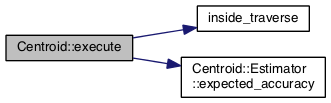
\includegraphics[width=320pt]{namespace_centroid_aae279838f4de04965b126f2760d1c2cb_cgraph}
\end{center}
\end{figure}




Here is the caller graph for this function\+:
\nopagebreak
\begin{figure}[H]
\begin{center}
\leavevmode
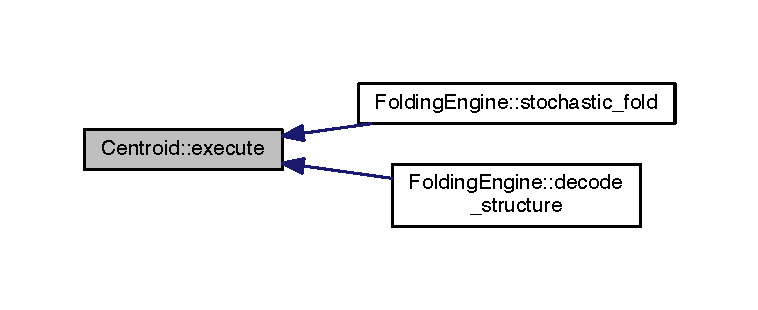
\includegraphics[width=350pt]{namespace_centroid_aae279838f4de04965b126f2760d1c2cb_icgraph}
\end{center}
\end{figure}


\hypertarget{namespace_centroid_a065a8778b18ed5997785ee42f45c4b9f}{\index{Centroid@{Centroid}!execute@{execute}}
\index{execute@{execute}!Centroid@{Centroid}}
\subsubsection[{execute}]{\setlength{\rightskip}{0pt plus 5cm}template$<$class T $>$ float Centroid\+::execute (
\begin{DoxyParamCaption}
\item[{const T \&}]{table, }
\item[{std\+::string \&}]{paren, }
\item[{{\bf uint}}]{max\+\_\+dist, }
\item[{float}]{gamma}
\end{DoxyParamCaption}
)}}\label{namespace_centroid_a065a8778b18ed5997785ee42f45c4b9f}


Definition at line 205 of file centroid.\+cpp.



Here is the call graph for this function\+:
\nopagebreak
\begin{figure}[H]
\begin{center}
\leavevmode
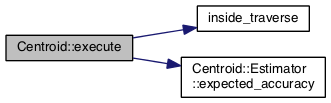
\includegraphics[width=320pt]{namespace_centroid_a065a8778b18ed5997785ee42f45c4b9f_cgraph}
\end{center}
\end{figure}



\hypertarget{namespace_c_o_n_t_r_a_l_i_g_n}{\section{C\+O\+N\+T\+R\+A\+L\+I\+G\+N Namespace Reference}
\label{namespace_c_o_n_t_r_a_l_i_g_n}\index{C\+O\+N\+T\+R\+A\+L\+I\+G\+N@{C\+O\+N\+T\+R\+A\+L\+I\+G\+N}}
}
\subsection*{Classes}
\begin{DoxyCompactItemize}
\item 
class \hyperlink{class_c_o_n_t_r_a_l_i_g_n_1_1_c_o_n_t_r_align}{C\+O\+N\+T\+R\+Align}
\item 
class \hyperlink{class_c_o_n_t_r_a_l_i_g_n_1_1_inference_engine}{Inference\+Engine}
\item 
class \hyperlink{class_c_o_n_t_r_a_l_i_g_n_1_1_multi_sequence}{Multi\+Sequence}
\item 
struct \hyperlink{struct_c_o_n_t_r_a_l_i_g_n_1_1_parameter_group}{Parameter\+Group}
\item 
class \hyperlink{class_c_o_n_t_r_a_l_i_g_n_1_1_parameter_manager}{Parameter\+Manager}
\item 
class \hyperlink{class_c_o_n_t_r_a_l_i_g_n_1_1_progressive}{Progressive}
\item 
class \hyperlink{class_c_o_n_t_r_a_l_i_g_n_1_1_sequence}{Sequence}
\item 
class \hyperlink{class_c_o_n_t_r_a_l_i_g_n_1_1_sparse_matrix}{Sparse\+Matrix}
\item 
struct \hyperlink{struct_c_o_n_t_r_a_l_i_g_n_1_1_sparse_matrix_entry}{Sparse\+Matrix\+Entry}
\item 
class \hyperlink{class_c_o_n_t_r_a_l_i_g_n_1_1_s_struct}{S\+Struct}
\item 
class \hyperlink{class_c_o_n_t_r_a_l_i_g_n_1_1_tree}{Tree}
\item 
struct \hyperlink{struct_c_o_n_t_r_a_l_i_g_n_1_1triple}{triple}
\end{DoxyCompactItemize}
\subsection*{Typedefs}
\begin{DoxyCompactItemize}
\item 
typedef unsigned char \hyperlink{namespace_c_o_n_t_r_a_l_i_g_n_a493b7d65e8378d6b823fd6332f1caa79}{B\+Y\+T\+E}
\end{DoxyCompactItemize}
\subsection*{Enumerations}
\begin{DoxyCompactItemize}
\item 
enum \hyperlink{namespace_c_o_n_t_r_a_l_i_g_n_a64bb6a3c7f6fb72e96a45b590f2fb825}{File\+Format} \{ \hyperlink{namespace_c_o_n_t_r_a_l_i_g_n_a64bb6a3c7f6fb72e96a45b590f2fb825a1978f4cc2e8d5cb064896f9be0f5f8df}{File\+Format\+\_\+\+F\+A\+S\+T\+A}, 
\hyperlink{namespace_c_o_n_t_r_a_l_i_g_n_a64bb6a3c7f6fb72e96a45b590f2fb825ac6b4ba8a4576509ebb7d1ebc69820cec}{File\+Format\+\_\+\+B\+P\+S\+E\+Q}, 
\hyperlink{namespace_c_o_n_t_r_a_l_i_g_n_a64bb6a3c7f6fb72e96a45b590f2fb825aef388571170761c3a03c13f7ce77e2ca}{File\+Format\+\_\+\+R\+A\+W}
 \}
\end{DoxyCompactItemize}
\subsection*{Functions}
\begin{DoxyCompactItemize}
\item 
void \hyperlink{namespace_c_o_n_t_r_a_l_i_g_n_a66c65550f4f2eb3b394af028bd34ff9d}{Usage} (const Options \&options)
\item 
void \hyperlink{namespace_c_o_n_t_r_a_l_i_g_n_afe20ba6958ee01585cc59f5561ec7d17}{Version} ()
\item 
void \hyperlink{namespace_c_o_n_t_r_a_l_i_g_n_a2d13a8e4ad05e8d6e2eb17d2b0a5850d}{Parse\+Arguments} (int argc, char $\ast$$\ast$argv, Options \&options, std\+::vector$<$ std\+::string $>$ \&filenames)
\item 
void \hyperlink{namespace_c_o_n_t_r_a_l_i_g_n_a749642fa4b12d011d9c7d00e0ceb6f0c}{Make\+File\+Descriptions} (const Options \&options, const std\+::vector$<$ std\+::string $>$ \&filenames, std\+::vector$<$ File\+Description $>$ \&descriptions)
\item 
{\footnotesize template$<$class Real\+T $>$ }\\void \hyperlink{namespace_c_o_n_t_r_a_l_i_g_n_a3bb2b00a11ab75abcaa97365ed5b4e60}{Run\+Gradient\+Sanity\+Check} (const Options \&options, const std\+::vector$<$ File\+Description $>$ \&descriptions)
\item 
{\footnotesize template$<$class Real\+T $>$ }\\void \hyperlink{namespace_c_o_n_t_r_a_l_i_g_n_a4ac70c3821db72a2c91f310a3d9ed454}{Run\+Training\+Mode} (const Options \&options, const std\+::vector$<$ File\+Description $>$ \&descriptions)
\item 
{\footnotesize template$<$class Real\+T $>$ }\\void \hyperlink{namespace_c_o_n_t_r_a_l_i_g_n_adcd53b6a98750eadf9d1a2230d0cab18}{Run\+Prediction\+Mode} (const Options \&options, const std\+::vector$<$ File\+Description $>$ \&descriptions)
\item 
int \hyperlink{namespace_c_o_n_t_r_a_l_i_g_n_aafc1edb6cd98e5858af45afee8327797}{\+\_\+main} (int argc, char $\ast$$\ast$argv)
\item 
{\footnotesize template$<$class Real\+T $>$ }\\std\+::vector$<$ Real\+T $>$ \hyperlink{namespace_c_o_n_t_r_a_l_i_g_n_af16f9793f865b3059ac02c8127cccb62}{Get\+Default\+Protein\+Values} ()
\item 
{\footnotesize template$<$class Real\+T $>$ }\\std\+::vector$<$ Real\+T $>$ \hyperlink{namespace_c_o_n_t_r_a_l_i_g_n_af0f740c7a84dffe3866c40f17e13b5f8}{Get\+Default\+R\+N\+A\+Values} ()
\item 
double \hyperlink{namespace_c_o_n_t_r_a_l_i_g_n_a0471adf771f411caa63052dc9d5dd7c0}{Fast\+\_\+\+Exp} (double x)
\item 
float \hyperlink{namespace_c_o_n_t_r_a_l_i_g_n_a00c672ebb0a129f6949436e11b4d2963}{Fast\+\_\+\+Exp} (float x)
\item 
double \hyperlink{namespace_c_o_n_t_r_a_l_i_g_n_ad082406a2c15bf172a3775ea2a21110d}{Fast\+\_\+\+Log\+Exp\+Plus\+One} (double x)
\item 
float \hyperlink{namespace_c_o_n_t_r_a_l_i_g_n_a4b02039d31911aca06afcd9378327353}{Fast\+\_\+\+Log\+Exp\+Plus\+One} (float x)
\item 
double \hyperlink{namespace_c_o_n_t_r_a_l_i_g_n_ac590e8506425b9a04fa9516a98a9475e}{Fast\+\_\+\+Log\+Exp\+Minus\+One} (double x)
\item 
float \hyperlink{namespace_c_o_n_t_r_a_l_i_g_n_aedd3ba0366cc273ba3ccc198f78e7415}{Fast\+\_\+\+Log\+Exp\+Minus\+One} (float x)
\item 
double \hyperlink{namespace_c_o_n_t_r_a_l_i_g_n_a7367cbf3b6f0971fe91f968df4e1ccfd}{Fast\+\_\+\+Log\+Add} (double x, double y)
\item 
float \hyperlink{namespace_c_o_n_t_r_a_l_i_g_n_a1f9990fb16821f775893785608a1828a}{Fast\+\_\+\+Log\+Add} (float x, float y)
\item 
void \hyperlink{namespace_c_o_n_t_r_a_l_i_g_n_a049b1ad00fa83ec722de8e96112840d0}{Fast\+\_\+\+Log\+Plus\+Equals} (double \&x, double y)
\item 
void \hyperlink{namespace_c_o_n_t_r_a_l_i_g_n_a3b315eff1e5eb5bb831046aa329b8f6a}{Fast\+\_\+\+Log\+Plus\+Equals} (float \&x, float y)
\item 
double \hyperlink{namespace_c_o_n_t_r_a_l_i_g_n_aa41663bbe3c2b32100e9025ff68eb7db}{Fast\+\_\+\+Log\+Subtract} (double x, double y)
\item 
float \hyperlink{namespace_c_o_n_t_r_a_l_i_g_n_ad85a3076602843900172f6a9579e7cde}{Fast\+\_\+\+Log\+Subtract} (float x, float y)
\item 
void \hyperlink{namespace_c_o_n_t_r_a_l_i_g_n_ac312a17e4a8d1e2cdcf973a8b219d31a}{Fast\+\_\+\+Log\+Minus\+Equals} (double \&x, double y)
\item 
void \hyperlink{namespace_c_o_n_t_r_a_l_i_g_n_a9cc2eca1e44a1a21f44bd44933281031}{Fast\+\_\+\+Log\+Minus\+Equals} (float \&x, float y)
\item 
int \hyperlink{namespace_c_o_n_t_r_a_l_i_g_n_a338a4c4e7404ab754609c2b78623a756}{\+\_\+\+A\+S\+S\+E\+R\+T\+\_\+\+F\+A\+I\+L\+E\+D} (const char $\ast$fmt,...)
\item 
void \hyperlink{namespace_c_o_n_t_r_a_l_i_g_n_a61966034d786cea05ffcfaf94857102b}{Error} (const char $\ast$fmt,...)
\item 
void \hyperlink{namespace_c_o_n_t_r_a_l_i_g_n_ac0f0da01d76aab8602edcd2e4defc15f}{Warning} (const char $\ast$fmt,...)
\item 
bool \hyperlink{namespace_c_o_n_t_r_a_l_i_g_n_a7d8b6bc69c474546641aca733a1ba0db}{Convert\+To\+Number} (const std\+::string \&s, int \&val)
\item 
bool \hyperlink{namespace_c_o_n_t_r_a_l_i_g_n_a7da237d8ce22882695f3c123458b86cc}{Convert\+To\+Number} (const std\+::string \&s, unsigned int \&val)
\item 
bool \hyperlink{namespace_c_o_n_t_r_a_l_i_g_n_a35c60ce0193bd02ab62b2a7a88cf28f8}{Convert\+To\+Number} (const std\+::string \&s, long int \&val)
\item 
bool \hyperlink{namespace_c_o_n_t_r_a_l_i_g_n_a6329df40493ff670585d485a8fa113c8}{Convert\+To\+Number} (const std\+::string \&s, unsigned long int \&val)
\item 
bool \hyperlink{namespace_c_o_n_t_r_a_l_i_g_n_af5c3734e0fb093eab48cb799bae2aaf8}{Convert\+To\+Number} (const std\+::string \&s, float \&val)
\item 
bool \hyperlink{namespace_c_o_n_t_r_a_l_i_g_n_a3808e83d03092912e19aedeb45b7c691}{Convert\+To\+Number} (const std\+::string \&s, double \&val)
\item 
bool \hyperlink{namespace_c_o_n_t_r_a_l_i_g_n_a7c45f697e83f0391b2af6b0e75f6f62f}{Convert\+To\+Number} (const std\+::string \&s, long double \&val)
\item 
std\+::string \hyperlink{namespace_c_o_n_t_r_a_l_i_g_n_aac140f1a8b0d61744322cd54dac36ddd}{Convert\+To\+Upper\+Case} (const std\+::string \&s)
\item 
std\+::string \hyperlink{namespace_c_o_n_t_r_a_l_i_g_n_a806aa2763d439f3199f571482ccd7033}{Convert\+To\+Lower\+Case} (const std\+::string \&s)
\item 
std\+::string \hyperlink{namespace_c_o_n_t_r_a_l_i_g_n_a9c5b90dd5ac218f263563dbd70e46e3d}{Trim} (const std\+::string \&s)
\item 
std\+::string \hyperlink{namespace_c_o_n_t_r_a_l_i_g_n_a00a7058454c235c938fb00a1f320ad79}{Remove\+Gaps} (const std\+::string \&s)
\item 
std\+::string \hyperlink{namespace_c_o_n_t_r_a_l_i_g_n_adeab7a5e03007b720dd6a7dc7bffd7de}{S\+Print\+F} (const char $\ast$fmt,...)
\item 
void \hyperlink{namespace_c_o_n_t_r_a_l_i_g_n_a8f97b6e8affaf0d7532a88095e5c0c39}{Write\+Progress\+Message} (const std\+::string \&message)
\item 
double \hyperlink{namespace_c_o_n_t_r_a_l_i_g_n_aa4152b19ef26d4c16d6b565b563286d1}{Get\+System\+Time} ()
\item 
void \hyperlink{namespace_c_o_n_t_r_a_l_i_g_n_a56cc93ad68a451ab0bd2681943a2116a}{Make\+Directory} (const std\+::string \&directory)
\item 
std\+::vector$<$ int $>$ \hyperlink{namespace_c_o_n_t_r_a_l_i_g_n_a09a6292733c57477e3ff079b192348d6}{Get\+Sequence\+Positions} (const std\+::string \&s)
\item 
std\+::vector$<$ int $>$ \hyperlink{namespace_c_o_n_t_r_a_l_i_g_n_a93f0680ae281198149502c325fc56d49}{Get\+Sequence\+Mapping} (const std\+::string \&s)
\item 
std\+::string \hyperlink{namespace_c_o_n_t_r_a_l_i_g_n_ac92d12442328b730b130b824cb8e71ba}{Get\+Dir\+Name} (const std\+::string \&filename)
\item 
std\+::string \hyperlink{namespace_c_o_n_t_r_a_l_i_g_n_aac8014733b9d18389b3e410cadf04539}{Get\+Base\+Name} (const std\+::string \&filename)
\item 
std\+::string \hyperlink{namespace_c_o_n_t_r_a_l_i_g_n_ae131464a4805f6186f3df734aed0b5ef}{Make\+Temp\+Directory} ()
\item 
int \hyperlink{namespace_c_o_n_t_r_a_l_i_g_n_ace866af1294f1def70aa7373adc6632d}{Ind} (bool condition)
\item 
{\footnotesize template$<$typename T1 , typename T2 , typename T3 $>$ }\\bool \hyperlink{namespace_c_o_n_t_r_a_l_i_g_n_aed9c0b72e8f62195682d84fb809bed28}{operator==} (const \hyperlink{struct_c_o_n_t_r_a_l_i_g_n_1_1triple}{triple}$<$ T1, T2, T3 $>$ \&x, const \hyperlink{struct_c_o_n_t_r_a_l_i_g_n_1_1triple}{triple}$<$ T1, T2, T3 $>$ \&y)
\item 
{\footnotesize template$<$typename T1 , typename T2 , typename T3 $>$ }\\bool \hyperlink{namespace_c_o_n_t_r_a_l_i_g_n_a00533aeff74d4937d55fc5325493000a}{operator$<$} (const \hyperlink{struct_c_o_n_t_r_a_l_i_g_n_1_1triple}{triple}$<$ T1, T2, T3 $>$ \&x, const \hyperlink{struct_c_o_n_t_r_a_l_i_g_n_1_1triple}{triple}$<$ T1, T2, T3 $>$ \&y)
\item 
{\footnotesize template$<$typename T1 , typename T2 , typename T3 $>$ }\\bool \hyperlink{namespace_c_o_n_t_r_a_l_i_g_n_a18792ba6906e25c2178227113f998924}{operator!=} (const \hyperlink{struct_c_o_n_t_r_a_l_i_g_n_1_1triple}{triple}$<$ T1, T2, T3 $>$ \&x, const \hyperlink{struct_c_o_n_t_r_a_l_i_g_n_1_1triple}{triple}$<$ T1, T2, T3 $>$ \&y)
\item 
{\footnotesize template$<$typename T1 , typename T2 , typename T3 $>$ }\\bool \hyperlink{namespace_c_o_n_t_r_a_l_i_g_n_ae3eb2ccb80d117e609ecc584ca71181f}{operator$>$} (const \hyperlink{struct_c_o_n_t_r_a_l_i_g_n_1_1triple}{triple}$<$ T1, T2, T3 $>$ \&x, const \hyperlink{struct_c_o_n_t_r_a_l_i_g_n_1_1triple}{triple}$<$ T1, T2, T3 $>$ \&y)
\item 
{\footnotesize template$<$typename T1 , typename T2 , typename T3 $>$ }\\bool \hyperlink{namespace_c_o_n_t_r_a_l_i_g_n_a8d549020d197328238ec07aec158d838}{operator$<$=} (const \hyperlink{struct_c_o_n_t_r_a_l_i_g_n_1_1triple}{triple}$<$ T1, T2, T3 $>$ \&x, const \hyperlink{struct_c_o_n_t_r_a_l_i_g_n_1_1triple}{triple}$<$ T1, T2, T3 $>$ \&y)
\item 
{\footnotesize template$<$typename T1 , typename T2 , typename T3 $>$ }\\bool \hyperlink{namespace_c_o_n_t_r_a_l_i_g_n_af2698ca3552c349853f1d45c74399d52}{operator$>$=} (const \hyperlink{struct_c_o_n_t_r_a_l_i_g_n_1_1triple}{triple}$<$ T1, T2, T3 $>$ \&x, const \hyperlink{struct_c_o_n_t_r_a_l_i_g_n_1_1triple}{triple}$<$ T1, T2, T3 $>$ \&y)
\item 
{\footnotesize template$<$typename T1 , typename T2 , typename T3 $>$ }\\\hyperlink{struct_c_o_n_t_r_a_l_i_g_n_1_1triple}{triple}$<$ T1, T2, T3 $>$ \hyperlink{namespace_c_o_n_t_r_a_l_i_g_n_a98175ddcaf753882eb5f92de09f9108f}{make\+\_\+triple} (T1 first, T2 second, T3 third)
\item 
{\footnotesize template$<$typename T1 , typename T2 $>$ }\\std\+::ostream \& \hyperlink{namespace_c_o_n_t_r_a_l_i_g_n_af60b1eb5579c95763c8241ab707b917e}{operator$<$$<$} (std\+::ostream \&out, const std\+::pair$<$ T1, T2 $>$ \&x)
\item 
{\footnotesize template$<$typename T1 , typename T2 , typename T3 $>$ }\\std\+::ostream \& \hyperlink{namespace_c_o_n_t_r_a_l_i_g_n_a37f6d4fc947c02293236890815321e35}{operator$<$$<$} (std\+::ostream \&out, const \hyperlink{struct_c_o_n_t_r_a_l_i_g_n_1_1triple}{triple}$<$ T1, T2, T3 $>$ \&x)
\item 
{\footnotesize template$<$typename T $>$ }\\T \hyperlink{namespace_c_o_n_t_r_a_l_i_g_n_ab021053662bde52f88f0e83578579559}{Sqrt} (const T x)
\item 
{\footnotesize template$<$typename T $>$ }\\T \hyperlink{namespace_c_o_n_t_r_a_l_i_g_n_a5ca67d3de567a8e208454433fc9b3985}{Exp} (const T x)
\item 
{\footnotesize template$<$typename T $>$ }\\T \hyperlink{namespace_c_o_n_t_r_a_l_i_g_n_a4bfa0bc3748b3484f0a9e0d9bb5a62fa}{Log} (const T x)
\item 
{\footnotesize template$<$typename T $>$ }\\T \hyperlink{namespace_c_o_n_t_r_a_l_i_g_n_a2c8a2f8551093619bdb7afa60d34db78}{Pow} (const T x, const T p)
\item 
{\footnotesize template$<$typename T $>$ }\\T \hyperlink{namespace_c_o_n_t_r_a_l_i_g_n_a054e3c2a248dca86c547d357c0063808}{Tanh} (const T x)
\item 
{\footnotesize template$<$typename T $>$ }\\T \hyperlink{namespace_c_o_n_t_r_a_l_i_g_n_a8eab454f786925da404894d345c55572}{Floor} (const T x)
\item 
{\footnotesize template$<$typename T $>$ }\\T \hyperlink{namespace_c_o_n_t_r_a_l_i_g_n_a71287d09e3234f79f410137964df4d2f}{Ceil} (const T x)
\item 
{\footnotesize template$<$typename T $>$ }\\T \hyperlink{namespace_c_o_n_t_r_a_l_i_g_n_ac6566074a120c798141a91753c50290f}{Abs} (const T x)
\item 
{\footnotesize template$<$typename T $>$ }\\T \hyperlink{namespace_c_o_n_t_r_a_l_i_g_n_aa4f87aa569c6cb44a0e15a73cc475c13}{Sign} (const T x)
\item 
{\footnotesize template$<$typename T $>$ }\\T \hyperlink{namespace_c_o_n_t_r_a_l_i_g_n_a469955594da581dc70e2bafc9f235680}{Clip} (const T x, const T lower, const T upper)
\item 
{\footnotesize template$<$typename T $>$ }\\T \hyperlink{namespace_c_o_n_t_r_a_l_i_g_n_a060f37f304d3b409ad044d105b37c4af}{Dot\+Product} (const std\+::vector$<$ T $>$ \&x, const std\+::vector$<$ T $>$ \&y)
\item 
{\footnotesize template$<$typename T $>$ }\\T \hyperlink{namespace_c_o_n_t_r_a_l_i_g_n_aea939de28045df5b9199ff4bf6a93b49}{Norm} (const std\+::vector$<$ T $>$ \&x)
\item 
{\footnotesize template$<$typename T $>$ }\\std\+::vector$<$ T $>$ \hyperlink{namespace_c_o_n_t_r_a_l_i_g_n_a816d76c04970024e87d6a1f9a683b5f6}{Sqrt} (const std\+::vector$<$ T $>$ \&x)
\item 
{\footnotesize template$<$typename T $>$ }\\std\+::vector$<$ T $>$ \hyperlink{namespace_c_o_n_t_r_a_l_i_g_n_a0c42332331fc02304c24391c147101aa}{Exp} (const std\+::vector$<$ T $>$ \&x)
\item 
{\footnotesize template$<$typename T $>$ }\\std\+::vector$<$ T $>$ \hyperlink{namespace_c_o_n_t_r_a_l_i_g_n_a2a61e9203cab173f040a408cf9dd9fff}{Log} (const std\+::vector$<$ T $>$ \&x)
\item 
{\footnotesize template$<$typename T $>$ }\\std\+::vector$<$ T $>$ \hyperlink{namespace_c_o_n_t_r_a_l_i_g_n_a17fe7e289f4cde741880207b3acc4130}{Pow} (const std\+::vector$<$ T $>$ \&x, const T p)
\item 
{\footnotesize template$<$typename T $>$ }\\std\+::vector$<$ T $>$ \hyperlink{namespace_c_o_n_t_r_a_l_i_g_n_a2bd0fc4d043cea02c1208cc7a6e43d22}{Tanh} (const std\+::vector$<$ T $>$ \&x)
\item 
{\footnotesize template$<$typename T $>$ }\\std\+::vector$<$ T $>$ \hyperlink{namespace_c_o_n_t_r_a_l_i_g_n_a881da0309b37d990b01dada1819b5d6f}{Abs} (const std\+::vector$<$ T $>$ \&x)
\item 
{\footnotesize template$<$typename T $>$ }\\std\+::vector$<$ T $>$ \hyperlink{namespace_c_o_n_t_r_a_l_i_g_n_aad158156e3616501f89ee66af1cf66ee}{Sign} (const std\+::vector$<$ T $>$ \&x)
\item 
{\footnotesize template$<$typename T , typename P $>$ }\\std\+::vector$<$ T $>$ \hyperlink{namespace_c_o_n_t_r_a_l_i_g_n_a75011b634203a445b81adaf2684162ff}{Test} (const std\+::vector$<$ T $>$ \&x, \hyperlink{pf__duplex_8c_a54f9e847235c2061dfd403c5869b5e2d}{P} pred)
\item 
{\footnotesize template$<$typename T $>$ }\\T \hyperlink{namespace_c_o_n_t_r_a_l_i_g_n_af5acb97fd09c707d30b0ba3a2f4ce343}{Sum} (const std\+::vector$<$ T $>$ \&x)
\item 
{\footnotesize template$<$typename T $>$ }\\T \hyperlink{namespace_c_o_n_t_r_a_l_i_g_n_ad582c5d78b26a7e58ee7721a42c01da6}{Prod} (const std\+::vector$<$ T $>$ \&x)
\item 
{\footnotesize template$<$typename T $>$ }\\const std\+::vector$<$ T $>$ \hyperlink{namespace_c_o_n_t_r_a_l_i_g_n_a6b53b3062ca847fb117cf013785f8100}{Min} (const std\+::vector$<$ T $>$ \&x, const T \&y)
\item 
{\footnotesize template$<$typename T $>$ }\\const std\+::vector$<$ T $>$ \hyperlink{namespace_c_o_n_t_r_a_l_i_g_n_a6c722fe0306d541389530e375d74ccdf}{Max} (const std\+::vector$<$ T $>$ \&x, const T \&y)
\item 
{\footnotesize template$<$typename T $>$ }\\const std\+::vector$<$ T $>$ \hyperlink{namespace_c_o_n_t_r_a_l_i_g_n_adf2697aa2857fa99795263160b364d3a}{Clip} (const std\+::vector$<$ T $>$ \&x, const T \&lower, const T \&upper)
\item 
{\footnotesize template$<$typename T $>$ }\\const std\+::vector$<$ T $>$ \hyperlink{namespace_c_o_n_t_r_a_l_i_g_n_a29e5e02d8c9a594a18989dd70a67d960}{Min} (const T \&x, const std\+::vector$<$ T $>$ \&y)
\item 
{\footnotesize template$<$typename T $>$ }\\const std\+::vector$<$ T $>$ \hyperlink{namespace_c_o_n_t_r_a_l_i_g_n_a5cc9c10aa252a488e82c2bb32c183747}{Max} (const T \&x, const std\+::vector$<$ T $>$ \&y)
\item 
{\footnotesize template$<$typename T $>$ }\\T \hyperlink{namespace_c_o_n_t_r_a_l_i_g_n_a1b53d2a84cfba4108bb7beb5270fe1c1}{Min} (const std\+::vector$<$ T $>$ \&x)
\item 
{\footnotesize template$<$typename T $>$ }\\T \hyperlink{namespace_c_o_n_t_r_a_l_i_g_n_a7a9aa6d2e9f21b56e04c47dc9bda0a12}{Max} (const std\+::vector$<$ T $>$ \&x)
\item 
{\footnotesize template$<$typename T $>$ }\\int \hyperlink{namespace_c_o_n_t_r_a_l_i_g_n_ab012f896d978a3dffc160298b00000be}{Arg\+Min} (const std\+::vector$<$ T $>$ \&x)
\item 
{\footnotesize template$<$typename T $>$ }\\int \hyperlink{namespace_c_o_n_t_r_a_l_i_g_n_a00dc218b758ac62148b43b448dc0c1c2}{Arg\+Max} (const std\+::vector$<$ T $>$ \&x)
\item 
{\footnotesize template$<$typename T $>$ }\\const std\+::vector$<$ T $>$ \hyperlink{namespace_c_o_n_t_r_a_l_i_g_n_a0dde76d72fb93b92bcf6bdcafbc435ba}{operator-\/} (const std\+::vector$<$ T $>$ \&x)
\item 
{\footnotesize template$<$typename T $>$ }\\const std\+::vector$<$ T $>$ \hyperlink{namespace_c_o_n_t_r_a_l_i_g_n_af1b254c31a46ad2861442bb2390ee336}{operator$\ast$} (const std\+::vector$<$ T $>$ \&x, const std\+::vector$<$ T $>$ \&y)
\item 
{\footnotesize template$<$typename T $>$ }\\const std\+::vector$<$ T $>$ \hyperlink{namespace_c_o_n_t_r_a_l_i_g_n_abe533e779b3a764b4b7dca6b627c1fed}{operator/} (const std\+::vector$<$ T $>$ \&x, const std\+::vector$<$ T $>$ \&y)
\item 
{\footnotesize template$<$typename T $>$ }\\const std\+::vector$<$ T $>$ \hyperlink{namespace_c_o_n_t_r_a_l_i_g_n_ad37632aa6d04b0b0735dfe1a104a1010}{operator+} (const std\+::vector$<$ T $>$ \&x, const std\+::vector$<$ T $>$ \&y)
\item 
{\footnotesize template$<$typename T $>$ }\\const std\+::vector$<$ T $>$ \hyperlink{namespace_c_o_n_t_r_a_l_i_g_n_a2a3a5dcf2fc4605559fa475cab65c6fe}{operator-\/} (const std\+::vector$<$ T $>$ \&x, const std\+::vector$<$ T $>$ \&y)
\item 
{\footnotesize template$<$typename T $>$ }\\const std\+::vector$<$ T $>$ \hyperlink{namespace_c_o_n_t_r_a_l_i_g_n_ae2d8e5fded025a34e09c65c2dc997dd8}{operator$\ast$} (const std\+::vector$<$ T $>$ \&x, const T \&y)
\item 
{\footnotesize template$<$typename T $>$ }\\const std\+::vector$<$ T $>$ \hyperlink{namespace_c_o_n_t_r_a_l_i_g_n_a2dca0d21c43b77c6ea3f790feb7ec634}{operator/} (const std\+::vector$<$ T $>$ \&x, const T \&y)
\item 
{\footnotesize template$<$typename T $>$ }\\const std\+::vector$<$ T $>$ \hyperlink{namespace_c_o_n_t_r_a_l_i_g_n_ae2222d1e328d2c582c47a729bf9ebf42}{operator+} (const std\+::vector$<$ T $>$ \&x, const T \&y)
\item 
{\footnotesize template$<$typename T $>$ }\\const std\+::vector$<$ T $>$ \hyperlink{namespace_c_o_n_t_r_a_l_i_g_n_a6999f279abf3d94291a284bc5b82546e}{operator-\/} (const std\+::vector$<$ T $>$ \&x, const T \&y)
\item 
{\footnotesize template$<$typename T $>$ }\\const std\+::vector$<$ T $>$ \hyperlink{namespace_c_o_n_t_r_a_l_i_g_n_a8b40f9b1bc2302cfd81508683105dd4f}{operator$\ast$} (const T \&x, const std\+::vector$<$ T $>$ \&y)
\item 
{\footnotesize template$<$typename T $>$ }\\const std\+::vector$<$ T $>$ \hyperlink{namespace_c_o_n_t_r_a_l_i_g_n_a514e32eb89504fc0d503a0350ff381cb}{operator/} (const T \&x, const std\+::vector$<$ T $>$ \&y)
\item 
{\footnotesize template$<$typename T $>$ }\\const std\+::vector$<$ T $>$ \hyperlink{namespace_c_o_n_t_r_a_l_i_g_n_ac43e8f22ac47bc4ce841bfc8c3fd943a}{operator+} (const T \&x, const std\+::vector$<$ T $>$ \&y)
\item 
{\footnotesize template$<$typename T $>$ }\\const std\+::vector$<$ T $>$ \hyperlink{namespace_c_o_n_t_r_a_l_i_g_n_abf9d5632e8a4feaa3d5b254ac83ccd03}{operator-\/} (const T \&x, const std\+::vector$<$ T $>$ \&y)
\item 
{\footnotesize template$<$typename T $>$ }\\std\+::vector$<$ T $>$ \& \hyperlink{namespace_c_o_n_t_r_a_l_i_g_n_aafc1ce4aa4d97210186c358eec543740}{operator$\ast$=} (std\+::vector$<$ T $>$ \&x, const std\+::vector$<$ T $>$ \&y)
\item 
{\footnotesize template$<$typename T $>$ }\\std\+::vector$<$ T $>$ \& \hyperlink{namespace_c_o_n_t_r_a_l_i_g_n_a0100c7e8af5633fb403d3cbeee1f0dce}{operator/=} (std\+::vector$<$ T $>$ \&x, const std\+::vector$<$ T $>$ \&y)
\item 
{\footnotesize template$<$typename T $>$ }\\std\+::vector$<$ T $>$ \& \hyperlink{namespace_c_o_n_t_r_a_l_i_g_n_ad2bf01877959caf081dbde8bac578f3f}{operator+=} (std\+::vector$<$ T $>$ \&x, const std\+::vector$<$ T $>$ \&y)
\item 
{\footnotesize template$<$typename T $>$ }\\std\+::vector$<$ T $>$ \& \hyperlink{namespace_c_o_n_t_r_a_l_i_g_n_af0e8c5f8fbce7e6a51b426e6ac663b30}{operator-\/=} (std\+::vector$<$ T $>$ \&x, const std\+::vector$<$ T $>$ \&y)
\item 
{\footnotesize template$<$typename T $>$ }\\std\+::vector$<$ T $>$ \& \hyperlink{namespace_c_o_n_t_r_a_l_i_g_n_a4da5ff7c4e30e9e3ac87eeecc67fb638}{operator$\ast$=} (std\+::vector$<$ T $>$ \&x, const T \&y)
\item 
{\footnotesize template$<$typename T $>$ }\\std\+::vector$<$ T $>$ \& \hyperlink{namespace_c_o_n_t_r_a_l_i_g_n_a821d8b72ad691f1e5b42ffe21b0c05d8}{operator/=} (std\+::vector$<$ T $>$ \&x, const T \&y)
\item 
{\footnotesize template$<$typename T $>$ }\\std\+::vector$<$ T $>$ \& \hyperlink{namespace_c_o_n_t_r_a_l_i_g_n_a9a01fa9073f79bc1871fd38aedeb8ac3}{operator+=} (std\+::vector$<$ T $>$ \&x, const T \&y)
\item 
{\footnotesize template$<$typename T $>$ }\\std\+::vector$<$ T $>$ \& \hyperlink{namespace_c_o_n_t_r_a_l_i_g_n_a47ed1e3a7df88433ef471e9ae68d8cdf}{operator-\/=} (std\+::vector$<$ T $>$ \&x, const T \&y)
\item 
{\footnotesize template$<$typename T $>$ }\\std\+::ostream \& \hyperlink{namespace_c_o_n_t_r_a_l_i_g_n_a837e827bff6e65e98e8c1cc9c2a34d28}{operator$<$$<$} (std\+::ostream \&out, const std\+::vector$<$ T $>$ \&x)
\item 
{\footnotesize template$<$typename T , typename U $>$ }\\std\+::vector$<$ T $>$ \hyperlink{namespace_c_o_n_t_r_a_l_i_g_n_a7482cc725c843303831d85acb4807163}{Convert\+Vector} (const std\+::vector$<$ U $>$ \&x)
\item 
{\footnotesize template$<$typename T $>$ }\\std\+::vector$<$ T $>$ \hyperlink{namespace_c_o_n_t_r_a_l_i_g_n_a1c2096f8a125b6a778f5fe8ef8c6b93a}{Concatenate} (const std\+::vector$<$ T $>$ \&u, const std\+::vector$<$ T $>$ \&v)
\item 
{\footnotesize template$<$typename T $>$ }\\std\+::vector$<$ T $>$ \hyperlink{namespace_c_o_n_t_r_a_l_i_g_n_ad43313a97ba0a47e7858d11c88f9da36}{Transpose} (const std\+::vector$<$ T $>$ \&m, const int rows, const int cols)
\item 
{\footnotesize template$<$class T $>$ }\\std\+::vector$<$ T $>$ \hyperlink{namespace_c_o_n_t_r_a_l_i_g_n_a53a2e031c10b47dedfcaab61f97c0c4b}{Expand\+Matrix} (const std\+::vector$<$ T $>$ \&mat, const int new\+\_\+rows, const int new\+\_\+cols, const std\+::vector$<$ int $>$ \&positions\+\_\+rows, const std\+::vector$<$ int $>$ \&positions\+\_\+cols)
\item 
{\footnotesize template$<$class T $>$ }\\std\+::vector$<$ T $>$ \hyperlink{namespace_c_o_n_t_r_a_l_i_g_n_a565dbfcc2a892a5a9d55c1dafc1a77bf}{Expand\+Vector} (const std\+::vector$<$ T $>$ \&v, const int new\+\_\+length, const std\+::vector$<$ int $>$ \&positions)
\item 
bool \hyperlink{namespace_c_o_n_t_r_a_l_i_g_n_adfeb25c8dd97c0d84c2b827e3d92e2e7}{Is\+Complementary} (char c, char d)
\item 
{\footnotesize template$<$$>$ }\\float \hyperlink{namespace_c_o_n_t_r_a_l_i_g_n_a5425dcac6298080e920d815d5181d13c}{Sqrt} (const float x)
\item 
{\footnotesize template$<$$>$ }\\double \hyperlink{namespace_c_o_n_t_r_a_l_i_g_n_aa5b0dc66ae5b9d211a2418219cd1e7a4}{Sqrt} (const double x)
\item 
{\footnotesize template$<$$>$ }\\long double \hyperlink{namespace_c_o_n_t_r_a_l_i_g_n_ab98bf329d8c67035829fa0055a84d591}{Sqrt} (const long double x)
\item 
{\footnotesize template$<$$>$ }\\float \hyperlink{namespace_c_o_n_t_r_a_l_i_g_n_aeaeb9f23b84ef5a3cb1f50056b205607}{Exp} (const float x)
\item 
{\footnotesize template$<$$>$ }\\double \hyperlink{namespace_c_o_n_t_r_a_l_i_g_n_a4f40660e51cb8debd179b0e375b8e9f0}{Exp} (const double x)
\item 
{\footnotesize template$<$$>$ }\\long double \hyperlink{namespace_c_o_n_t_r_a_l_i_g_n_a2f9f92ee735011a2f6864ff388a15ebe}{Exp} (const long double x)
\item 
{\footnotesize template$<$$>$ }\\float \hyperlink{namespace_c_o_n_t_r_a_l_i_g_n_a569ff2ac6f15afca32da99bc7c90a2ec}{Log} (const float x)
\item 
{\footnotesize template$<$$>$ }\\double \hyperlink{namespace_c_o_n_t_r_a_l_i_g_n_a42c87473a0bb7acac9a2ec85b8170c48}{Log} (const double x)
\item 
{\footnotesize template$<$$>$ }\\long double \hyperlink{namespace_c_o_n_t_r_a_l_i_g_n_a203566733c1db741c04c8ba43bfac9f2}{Log} (const long double x)
\item 
{\footnotesize template$<$$>$ }\\float \hyperlink{namespace_c_o_n_t_r_a_l_i_g_n_a84be357ebad35b3bc5c1f868eae5a880}{Pow} (const float x, const float p)
\item 
{\footnotesize template$<$$>$ }\\double \hyperlink{namespace_c_o_n_t_r_a_l_i_g_n_ab3f0a54836ccd297d5bbe337f191943a}{Pow} (const double x, const double p)
\item 
{\footnotesize template$<$$>$ }\\long double \hyperlink{namespace_c_o_n_t_r_a_l_i_g_n_ae1f4a55e11316f304596d3a26869d375}{Pow} (const long double x, const long double p)
\item 
{\footnotesize template$<$$>$ }\\float \hyperlink{namespace_c_o_n_t_r_a_l_i_g_n_acf91d891dabcc9c64740f9f97d3e30d1}{Tanh} (const float x)
\item 
{\footnotesize template$<$$>$ }\\double \hyperlink{namespace_c_o_n_t_r_a_l_i_g_n_a647e44a28c6fa1922856f72076098ae4}{Tanh} (const double x)
\item 
{\footnotesize template$<$$>$ }\\long double \hyperlink{namespace_c_o_n_t_r_a_l_i_g_n_aec2280338a362a451b5d959dc6e2fd97}{Tanh} (const long double x)
\item 
{\footnotesize template$<$$>$ }\\float \hyperlink{namespace_c_o_n_t_r_a_l_i_g_n_a57c956df884afde3839cbcff1a8569a9}{Floor} (const float x)
\item 
{\footnotesize template$<$$>$ }\\double \hyperlink{namespace_c_o_n_t_r_a_l_i_g_n_aad3a78d6112cc443813287d60afa95a2}{Floor} (const double x)
\item 
{\footnotesize template$<$$>$ }\\long double \hyperlink{namespace_c_o_n_t_r_a_l_i_g_n_a80f1355ab7b7bb9ad01c2a1ac800833f}{Floor} (const long double x)
\item 
{\footnotesize template$<$$>$ }\\float \hyperlink{namespace_c_o_n_t_r_a_l_i_g_n_afd0532ccadde7e7c48ee5bcc64693122}{Ceil} (const float x)
\item 
{\footnotesize template$<$$>$ }\\double \hyperlink{namespace_c_o_n_t_r_a_l_i_g_n_ac39c37f6c9451024a010d4821c1c1607}{Ceil} (const double x)
\item 
{\footnotesize template$<$$>$ }\\long double \hyperlink{namespace_c_o_n_t_r_a_l_i_g_n_aa275ad45d22c758e8f3a98f0804f91ea}{Ceil} (const long double x)
\end{DoxyCompactItemize}
\subsection*{Variables}
\begin{DoxyCompactItemize}
\item 
const int \hyperlink{namespace_c_o_n_t_r_a_l_i_g_n_ac55874d60f48cb644c7c65c79dcb2d54}{S\+H\+A\+R\+E\+D\+\_\+\+P\+A\+R\+A\+M\+E\+T\+E\+R\+\_\+\+S\+I\+Z\+E} = 5000
\item 
const double \hyperlink{namespace_c_o_n_t_r_a_l_i_g_n_a8574a561e08eaaaaf2caa651732430ef}{N\+O\+N\+C\+O\+N\+V\+E\+X\+\_\+\+M\+U\+L\+T\+I\+P\+L\+I\+E\+R} = 0.\+0
\item 
const int \hyperlink{namespace_c_o_n_t_r_a_l_i_g_n_a3299389049ee38f5124c6da1d99fe81e}{N\+U\+M\+\_\+\+C\+C\+C\+P\+\_\+\+S\+T\+E\+P\+S} = 5
\item 
const double \hyperlink{namespace_c_o_n_t_r_a_l_i_g_n_aeee5c8bdae11d43911362af4a21348a8}{I\+N\+I\+T\+I\+A\+L\+\_\+\+L\+O\+G\+\_\+\+C} = 5.\+0
\item 
const int \hyperlink{namespace_c_o_n_t_r_a_l_i_g_n_a6a3b0669d404c530e542b95d555ce89b}{N\+U\+M\+\_\+\+I\+T\+E\+R\+A\+T\+I\+V\+E\+\_\+\+R\+E\+L\+I\+N\+E\+A\+R\+I\+Z\+A\+T\+I\+O\+N\+\_\+\+S\+T\+E\+P\+S} = 5
\item 
const double \hyperlink{namespace_c_o_n_t_r_a_l_i_g_n_a5526bbb095dad1642772b911061636e9}{M\+M\+\_\+\+S\+M\+O\+O\+T\+H\+I\+N\+G} = 1.\+0
\item 
const std\+::string \hyperlink{namespace_c_o_n_t_r_a_l_i_g_n_a2ff97191ea8854b1801441553af77857}{alphabet} = \char`\"{}A\+R\+N\+D\+C\+Q\+E\+G\+H\+I\+L\+K\+M\+F\+P\+S\+T\+W\+Y\+V\+B\+Z\+X\char`\"{}
\item 
const int \hyperlink{namespace_c_o_n_t_r_a_l_i_g_n_a7ce1fa1c6c36bd3bda0f8b508e6d8905}{M} = 23
\item 
const std\+::string \hyperlink{namespace_c_o_n_t_r_a_l_i_g_n_a01d91421b64dd93348343bcaa3b2bedc}{hydrophilic\+\_\+alphabet} = \char`\"{}D\+E\+G\+K\+N\+Q\+P\+R\+S\char`\"{}
\item 
const int \hyperlink{namespace_c_o_n_t_r_a_l_i_g_n_aaacc59b31308cc741658a6209609157b}{H} = 6
\item 
const int \hyperlink{namespace_c_o_n_t_r_a_l_i_g_n_a28d4592514704ed3e73d954d34bd4128}{C\+O\+M\+P\+R\+E\+S\+S\+E\+D\+\_\+\+M} = 6
\item 
const std\+::string \hyperlink{namespace_c_o_n_t_r_a_l_i_g_n_abc81d204924eda147b14d8d4da2b3f21}{compressed\+\_\+alphabet} \mbox{[}\hyperlink{namespace_c_o_n_t_r_a_l_i_g_n_a28d4592514704ed3e73d954d34bd4128}{C\+O\+M\+P\+R\+E\+S\+S\+E\+D\+\_\+\+M}\mbox{]} = \{\char`\"{}A\+G\+P\+S\+T\char`\"{}, \char`\"{}C\char`\"{}, \char`\"{}D\+E\+N\+Q\char`\"{}, \char`\"{}F\+W\+Y\char`\"{}, \char`\"{}H\+K\+R\char`\"{}, \char`\"{}I\+L\+M\+V\char`\"{}\}
\item 
const double \hyperlink{namespace_c_o_n_t_r_a_l_i_g_n_acc27a8d5de00a0e2b28341a554b1671e}{G\+A\+M\+M\+A\+\_\+\+D\+E\+F\+A\+U\+L\+T} = 100000
\item 
const double \hyperlink{namespace_c_o_n_t_r_a_l_i_g_n_ab8d1796ab4c3172fefb62e6551fc0e6a}{R\+E\+G\+U\+L\+A\+R\+I\+Z\+A\+T\+I\+O\+N\+\_\+\+D\+E\+F\+A\+U\+L\+T} = 0
\item 
const int \hyperlink{namespace_c_o_n_t_r_a_l_i_g_n_a7eae27d13bfe8d19d465e4e02325b7ca}{P\+C\+\_\+\+I\+T\+E\+R\+S\+\_\+\+D\+E\+F\+A\+U\+L\+T} = 2
\item 
const int \hyperlink{namespace_c_o_n_t_r_a_l_i_g_n_a5d28e8f24c1100580fce7418871aab48}{S\+C\+\_\+\+I\+T\+E\+R\+S\+\_\+\+D\+E\+F\+A\+U\+L\+T} = 0
\item 
bool \hyperlink{namespace_c_o_n_t_r_a_l_i_g_n_ab3c518611777e6b169ba6c8f0fadfc9d}{toggle\+\_\+error} = \hyperlink{naview_8c_a65e9886d74aaee76545e83dd09011727}{false}
\item 
const char \hyperlink{namespace_c_o_n_t_r_a_l_i_g_n_a10799300da481510c609583326c3bcaa}{D\+I\+R\+\_\+\+S\+E\+P\+A\+R\+A\+T\+O\+R\+\_\+\+C\+H\+A\+R} = '/'
\end{DoxyCompactItemize}


\subsection{Typedef Documentation}
\hypertarget{namespace_c_o_n_t_r_a_l_i_g_n_a493b7d65e8378d6b823fd6332f1caa79}{\index{C\+O\+N\+T\+R\+A\+L\+I\+G\+N@{C\+O\+N\+T\+R\+A\+L\+I\+G\+N}!B\+Y\+T\+E@{B\+Y\+T\+E}}
\index{B\+Y\+T\+E@{B\+Y\+T\+E}!C\+O\+N\+T\+R\+A\+L\+I\+G\+N@{C\+O\+N\+T\+R\+A\+L\+I\+G\+N}}
\subsubsection[{B\+Y\+T\+E}]{\setlength{\rightskip}{0pt plus 5cm}typedef unsigned char {\bf C\+O\+N\+T\+R\+A\+L\+I\+G\+N\+::\+B\+Y\+T\+E}}}\label{namespace_c_o_n_t_r_a_l_i_g_n_a493b7d65e8378d6b823fd6332f1caa79}


\subsection{Enumeration Type Documentation}
\hypertarget{namespace_c_o_n_t_r_a_l_i_g_n_a64bb6a3c7f6fb72e96a45b590f2fb825}{\index{C\+O\+N\+T\+R\+A\+L\+I\+G\+N@{C\+O\+N\+T\+R\+A\+L\+I\+G\+N}!File\+Format@{File\+Format}}
\index{File\+Format@{File\+Format}!C\+O\+N\+T\+R\+A\+L\+I\+G\+N@{C\+O\+N\+T\+R\+A\+L\+I\+G\+N}}
\subsubsection[{File\+Format}]{\setlength{\rightskip}{0pt plus 5cm}enum {\bf C\+O\+N\+T\+R\+A\+L\+I\+G\+N\+::\+File\+Format}}}\label{namespace_c_o_n_t_r_a_l_i_g_n_a64bb6a3c7f6fb72e96a45b590f2fb825}
\begin{Desc}
\item[Enumerator]\par
\begin{description}
\index{File\+Format\+\_\+\+F\+A\+S\+T\+A@{File\+Format\+\_\+\+F\+A\+S\+T\+A}!C\+O\+N\+T\+R\+A\+L\+I\+G\+N@{C\+O\+N\+T\+R\+A\+L\+I\+G\+N}}\index{C\+O\+N\+T\+R\+A\+L\+I\+G\+N@{C\+O\+N\+T\+R\+A\+L\+I\+G\+N}!File\+Format\+\_\+\+F\+A\+S\+T\+A@{File\+Format\+\_\+\+F\+A\+S\+T\+A}}\item[{\em 
\hypertarget{namespace_c_o_n_t_r_a_l_i_g_n_a64bb6a3c7f6fb72e96a45b590f2fb825a1978f4cc2e8d5cb064896f9be0f5f8df}{File\+Format\+\_\+\+F\+A\+S\+T\+A}\label{namespace_c_o_n_t_r_a_l_i_g_n_a64bb6a3c7f6fb72e96a45b590f2fb825a1978f4cc2e8d5cb064896f9be0f5f8df}
}]\index{File\+Format\+\_\+\+B\+P\+S\+E\+Q@{File\+Format\+\_\+\+B\+P\+S\+E\+Q}!C\+O\+N\+T\+R\+A\+L\+I\+G\+N@{C\+O\+N\+T\+R\+A\+L\+I\+G\+N}}\index{C\+O\+N\+T\+R\+A\+L\+I\+G\+N@{C\+O\+N\+T\+R\+A\+L\+I\+G\+N}!File\+Format\+\_\+\+B\+P\+S\+E\+Q@{File\+Format\+\_\+\+B\+P\+S\+E\+Q}}\item[{\em 
\hypertarget{namespace_c_o_n_t_r_a_l_i_g_n_a64bb6a3c7f6fb72e96a45b590f2fb825ac6b4ba8a4576509ebb7d1ebc69820cec}{File\+Format\+\_\+\+B\+P\+S\+E\+Q}\label{namespace_c_o_n_t_r_a_l_i_g_n_a64bb6a3c7f6fb72e96a45b590f2fb825ac6b4ba8a4576509ebb7d1ebc69820cec}
}]\index{File\+Format\+\_\+\+R\+A\+W@{File\+Format\+\_\+\+R\+A\+W}!C\+O\+N\+T\+R\+A\+L\+I\+G\+N@{C\+O\+N\+T\+R\+A\+L\+I\+G\+N}}\index{C\+O\+N\+T\+R\+A\+L\+I\+G\+N@{C\+O\+N\+T\+R\+A\+L\+I\+G\+N}!File\+Format\+\_\+\+R\+A\+W@{File\+Format\+\_\+\+R\+A\+W}}\item[{\em 
\hypertarget{namespace_c_o_n_t_r_a_l_i_g_n_a64bb6a3c7f6fb72e96a45b590f2fb825aef388571170761c3a03c13f7ce77e2ca}{File\+Format\+\_\+\+R\+A\+W}\label{namespace_c_o_n_t_r_a_l_i_g_n_a64bb6a3c7f6fb72e96a45b590f2fb825aef388571170761c3a03c13f7ce77e2ca}
}]\end{description}
\end{Desc}


\subsection{Function Documentation}
\hypertarget{namespace_c_o_n_t_r_a_l_i_g_n_a338a4c4e7404ab754609c2b78623a756}{\index{C\+O\+N\+T\+R\+A\+L\+I\+G\+N@{C\+O\+N\+T\+R\+A\+L\+I\+G\+N}!\+\_\+\+A\+S\+S\+E\+R\+T\+\_\+\+F\+A\+I\+L\+E\+D@{\+\_\+\+A\+S\+S\+E\+R\+T\+\_\+\+F\+A\+I\+L\+E\+D}}
\index{\+\_\+\+A\+S\+S\+E\+R\+T\+\_\+\+F\+A\+I\+L\+E\+D@{\+\_\+\+A\+S\+S\+E\+R\+T\+\_\+\+F\+A\+I\+L\+E\+D}!C\+O\+N\+T\+R\+A\+L\+I\+G\+N@{C\+O\+N\+T\+R\+A\+L\+I\+G\+N}}
\subsubsection[{\+\_\+\+A\+S\+S\+E\+R\+T\+\_\+\+F\+A\+I\+L\+E\+D}]{\setlength{\rightskip}{0pt plus 5cm}int C\+O\+N\+T\+R\+A\+L\+I\+G\+N\+::\+\_\+\+A\+S\+S\+E\+R\+T\+\_\+\+F\+A\+I\+L\+E\+D (
\begin{DoxyParamCaption}
\item[{const char $\ast$}]{fmt, }
\item[{}]{...}
\end{DoxyParamCaption}
)}}\label{namespace_c_o_n_t_r_a_l_i_g_n_a338a4c4e7404ab754609c2b78623a756}
\hypertarget{namespace_c_o_n_t_r_a_l_i_g_n_aafc1edb6cd98e5858af45afee8327797}{\index{C\+O\+N\+T\+R\+A\+L\+I\+G\+N@{C\+O\+N\+T\+R\+A\+L\+I\+G\+N}!\+\_\+main@{\+\_\+main}}
\index{\+\_\+main@{\+\_\+main}!C\+O\+N\+T\+R\+A\+L\+I\+G\+N@{C\+O\+N\+T\+R\+A\+L\+I\+G\+N}}
\subsubsection[{\+\_\+main}]{\setlength{\rightskip}{0pt plus 5cm}int C\+O\+N\+T\+R\+A\+L\+I\+G\+N\+::\+\_\+main (
\begin{DoxyParamCaption}
\item[{int}]{argc, }
\item[{char $\ast$$\ast$}]{argv}
\end{DoxyParamCaption}
)}}\label{namespace_c_o_n_t_r_a_l_i_g_n_aafc1edb6cd98e5858af45afee8327797}
\hypertarget{namespace_c_o_n_t_r_a_l_i_g_n_ac6566074a120c798141a91753c50290f}{\index{C\+O\+N\+T\+R\+A\+L\+I\+G\+N@{C\+O\+N\+T\+R\+A\+L\+I\+G\+N}!Abs@{Abs}}
\index{Abs@{Abs}!C\+O\+N\+T\+R\+A\+L\+I\+G\+N@{C\+O\+N\+T\+R\+A\+L\+I\+G\+N}}
\subsubsection[{Abs}]{\setlength{\rightskip}{0pt plus 5cm}template$<$typename T $>$ T C\+O\+N\+T\+R\+A\+L\+I\+G\+N\+::\+Abs (
\begin{DoxyParamCaption}
\item[{const T}]{x}
\end{DoxyParamCaption}
)}}\label{namespace_c_o_n_t_r_a_l_i_g_n_ac6566074a120c798141a91753c50290f}
\hypertarget{namespace_c_o_n_t_r_a_l_i_g_n_a881da0309b37d990b01dada1819b5d6f}{\index{C\+O\+N\+T\+R\+A\+L\+I\+G\+N@{C\+O\+N\+T\+R\+A\+L\+I\+G\+N}!Abs@{Abs}}
\index{Abs@{Abs}!C\+O\+N\+T\+R\+A\+L\+I\+G\+N@{C\+O\+N\+T\+R\+A\+L\+I\+G\+N}}
\subsubsection[{Abs}]{\setlength{\rightskip}{0pt plus 5cm}template$<$typename T $>$ std\+::vector$<$ T $>$ C\+O\+N\+T\+R\+A\+L\+I\+G\+N\+::\+Abs (
\begin{DoxyParamCaption}
\item[{const std\+::vector$<$ T $>$ \&}]{x}
\end{DoxyParamCaption}
)}}\label{namespace_c_o_n_t_r_a_l_i_g_n_a881da0309b37d990b01dada1819b5d6f}
\hypertarget{namespace_c_o_n_t_r_a_l_i_g_n_a00dc218b758ac62148b43b448dc0c1c2}{\index{C\+O\+N\+T\+R\+A\+L\+I\+G\+N@{C\+O\+N\+T\+R\+A\+L\+I\+G\+N}!Arg\+Max@{Arg\+Max}}
\index{Arg\+Max@{Arg\+Max}!C\+O\+N\+T\+R\+A\+L\+I\+G\+N@{C\+O\+N\+T\+R\+A\+L\+I\+G\+N}}
\subsubsection[{Arg\+Max}]{\setlength{\rightskip}{0pt plus 5cm}template$<$typename T $>$ int C\+O\+N\+T\+R\+A\+L\+I\+G\+N\+::\+Arg\+Max (
\begin{DoxyParamCaption}
\item[{const std\+::vector$<$ T $>$ \&}]{x}
\end{DoxyParamCaption}
)}}\label{namespace_c_o_n_t_r_a_l_i_g_n_a00dc218b758ac62148b43b448dc0c1c2}
\hypertarget{namespace_c_o_n_t_r_a_l_i_g_n_ab012f896d978a3dffc160298b00000be}{\index{C\+O\+N\+T\+R\+A\+L\+I\+G\+N@{C\+O\+N\+T\+R\+A\+L\+I\+G\+N}!Arg\+Min@{Arg\+Min}}
\index{Arg\+Min@{Arg\+Min}!C\+O\+N\+T\+R\+A\+L\+I\+G\+N@{C\+O\+N\+T\+R\+A\+L\+I\+G\+N}}
\subsubsection[{Arg\+Min}]{\setlength{\rightskip}{0pt plus 5cm}template$<$typename T $>$ int C\+O\+N\+T\+R\+A\+L\+I\+G\+N\+::\+Arg\+Min (
\begin{DoxyParamCaption}
\item[{const std\+::vector$<$ T $>$ \&}]{x}
\end{DoxyParamCaption}
)}}\label{namespace_c_o_n_t_r_a_l_i_g_n_ab012f896d978a3dffc160298b00000be}
\hypertarget{namespace_c_o_n_t_r_a_l_i_g_n_afd0532ccadde7e7c48ee5bcc64693122}{\index{C\+O\+N\+T\+R\+A\+L\+I\+G\+N@{C\+O\+N\+T\+R\+A\+L\+I\+G\+N}!Ceil@{Ceil}}
\index{Ceil@{Ceil}!C\+O\+N\+T\+R\+A\+L\+I\+G\+N@{C\+O\+N\+T\+R\+A\+L\+I\+G\+N}}
\subsubsection[{Ceil}]{\setlength{\rightskip}{0pt plus 5cm}template$<$$>$ float C\+O\+N\+T\+R\+A\+L\+I\+G\+N\+::\+Ceil (
\begin{DoxyParamCaption}
\item[{const float}]{x}
\end{DoxyParamCaption}
)\hspace{0.3cm}{\ttfamily [inline]}}}\label{namespace_c_o_n_t_r_a_l_i_g_n_afd0532ccadde7e7c48ee5bcc64693122}
\hypertarget{namespace_c_o_n_t_r_a_l_i_g_n_ac39c37f6c9451024a010d4821c1c1607}{\index{C\+O\+N\+T\+R\+A\+L\+I\+G\+N@{C\+O\+N\+T\+R\+A\+L\+I\+G\+N}!Ceil@{Ceil}}
\index{Ceil@{Ceil}!C\+O\+N\+T\+R\+A\+L\+I\+G\+N@{C\+O\+N\+T\+R\+A\+L\+I\+G\+N}}
\subsubsection[{Ceil}]{\setlength{\rightskip}{0pt plus 5cm}template$<$$>$ double C\+O\+N\+T\+R\+A\+L\+I\+G\+N\+::\+Ceil (
\begin{DoxyParamCaption}
\item[{const double}]{x}
\end{DoxyParamCaption}
)\hspace{0.3cm}{\ttfamily [inline]}}}\label{namespace_c_o_n_t_r_a_l_i_g_n_ac39c37f6c9451024a010d4821c1c1607}
\hypertarget{namespace_c_o_n_t_r_a_l_i_g_n_aa275ad45d22c758e8f3a98f0804f91ea}{\index{C\+O\+N\+T\+R\+A\+L\+I\+G\+N@{C\+O\+N\+T\+R\+A\+L\+I\+G\+N}!Ceil@{Ceil}}
\index{Ceil@{Ceil}!C\+O\+N\+T\+R\+A\+L\+I\+G\+N@{C\+O\+N\+T\+R\+A\+L\+I\+G\+N}}
\subsubsection[{Ceil}]{\setlength{\rightskip}{0pt plus 5cm}template$<$$>$ long double C\+O\+N\+T\+R\+A\+L\+I\+G\+N\+::\+Ceil (
\begin{DoxyParamCaption}
\item[{const long double}]{x}
\end{DoxyParamCaption}
)\hspace{0.3cm}{\ttfamily [inline]}}}\label{namespace_c_o_n_t_r_a_l_i_g_n_aa275ad45d22c758e8f3a98f0804f91ea}
\hypertarget{namespace_c_o_n_t_r_a_l_i_g_n_a71287d09e3234f79f410137964df4d2f}{\index{C\+O\+N\+T\+R\+A\+L\+I\+G\+N@{C\+O\+N\+T\+R\+A\+L\+I\+G\+N}!Ceil@{Ceil}}
\index{Ceil@{Ceil}!C\+O\+N\+T\+R\+A\+L\+I\+G\+N@{C\+O\+N\+T\+R\+A\+L\+I\+G\+N}}
\subsubsection[{Ceil}]{\setlength{\rightskip}{0pt plus 5cm}template$<$typename T $>$ T C\+O\+N\+T\+R\+A\+L\+I\+G\+N\+::\+Ceil (
\begin{DoxyParamCaption}
\item[{const T}]{x}
\end{DoxyParamCaption}
)}}\label{namespace_c_o_n_t_r_a_l_i_g_n_a71287d09e3234f79f410137964df4d2f}
\hypertarget{namespace_c_o_n_t_r_a_l_i_g_n_a469955594da581dc70e2bafc9f235680}{\index{C\+O\+N\+T\+R\+A\+L\+I\+G\+N@{C\+O\+N\+T\+R\+A\+L\+I\+G\+N}!Clip@{Clip}}
\index{Clip@{Clip}!C\+O\+N\+T\+R\+A\+L\+I\+G\+N@{C\+O\+N\+T\+R\+A\+L\+I\+G\+N}}
\subsubsection[{Clip}]{\setlength{\rightskip}{0pt plus 5cm}template$<$typename T $>$ T C\+O\+N\+T\+R\+A\+L\+I\+G\+N\+::\+Clip (
\begin{DoxyParamCaption}
\item[{const T}]{x, }
\item[{const T}]{lower, }
\item[{const T}]{upper}
\end{DoxyParamCaption}
)\hspace{0.3cm}{\ttfamily [inline]}}}\label{namespace_c_o_n_t_r_a_l_i_g_n_a469955594da581dc70e2bafc9f235680}
\hypertarget{namespace_c_o_n_t_r_a_l_i_g_n_adf2697aa2857fa99795263160b364d3a}{\index{C\+O\+N\+T\+R\+A\+L\+I\+G\+N@{C\+O\+N\+T\+R\+A\+L\+I\+G\+N}!Clip@{Clip}}
\index{Clip@{Clip}!C\+O\+N\+T\+R\+A\+L\+I\+G\+N@{C\+O\+N\+T\+R\+A\+L\+I\+G\+N}}
\subsubsection[{Clip}]{\setlength{\rightskip}{0pt plus 5cm}template$<$typename T $>$ const std\+::vector$<$ T $>$ C\+O\+N\+T\+R\+A\+L\+I\+G\+N\+::\+Clip (
\begin{DoxyParamCaption}
\item[{const std\+::vector$<$ T $>$ \&}]{x, }
\item[{const T \&}]{lower, }
\item[{const T \&}]{upper}
\end{DoxyParamCaption}
)}}\label{namespace_c_o_n_t_r_a_l_i_g_n_adf2697aa2857fa99795263160b364d3a}
\hypertarget{namespace_c_o_n_t_r_a_l_i_g_n_a1c2096f8a125b6a778f5fe8ef8c6b93a}{\index{C\+O\+N\+T\+R\+A\+L\+I\+G\+N@{C\+O\+N\+T\+R\+A\+L\+I\+G\+N}!Concatenate@{Concatenate}}
\index{Concatenate@{Concatenate}!C\+O\+N\+T\+R\+A\+L\+I\+G\+N@{C\+O\+N\+T\+R\+A\+L\+I\+G\+N}}
\subsubsection[{Concatenate}]{\setlength{\rightskip}{0pt plus 5cm}template$<$typename T $>$ std\+::vector$<$ T $>$ C\+O\+N\+T\+R\+A\+L\+I\+G\+N\+::\+Concatenate (
\begin{DoxyParamCaption}
\item[{const std\+::vector$<$ T $>$ \&}]{u, }
\item[{const std\+::vector$<$ T $>$ \&}]{v}
\end{DoxyParamCaption}
)}}\label{namespace_c_o_n_t_r_a_l_i_g_n_a1c2096f8a125b6a778f5fe8ef8c6b93a}
\hypertarget{namespace_c_o_n_t_r_a_l_i_g_n_a806aa2763d439f3199f571482ccd7033}{\index{C\+O\+N\+T\+R\+A\+L\+I\+G\+N@{C\+O\+N\+T\+R\+A\+L\+I\+G\+N}!Convert\+To\+Lower\+Case@{Convert\+To\+Lower\+Case}}
\index{Convert\+To\+Lower\+Case@{Convert\+To\+Lower\+Case}!C\+O\+N\+T\+R\+A\+L\+I\+G\+N@{C\+O\+N\+T\+R\+A\+L\+I\+G\+N}}
\subsubsection[{Convert\+To\+Lower\+Case}]{\setlength{\rightskip}{0pt plus 5cm}std\+::string C\+O\+N\+T\+R\+A\+L\+I\+G\+N\+::\+Convert\+To\+Lower\+Case (
\begin{DoxyParamCaption}
\item[{const std\+::string \&}]{s}
\end{DoxyParamCaption}
)}}\label{namespace_c_o_n_t_r_a_l_i_g_n_a806aa2763d439f3199f571482ccd7033}
\hypertarget{namespace_c_o_n_t_r_a_l_i_g_n_a7d8b6bc69c474546641aca733a1ba0db}{\index{C\+O\+N\+T\+R\+A\+L\+I\+G\+N@{C\+O\+N\+T\+R\+A\+L\+I\+G\+N}!Convert\+To\+Number@{Convert\+To\+Number}}
\index{Convert\+To\+Number@{Convert\+To\+Number}!C\+O\+N\+T\+R\+A\+L\+I\+G\+N@{C\+O\+N\+T\+R\+A\+L\+I\+G\+N}}
\subsubsection[{Convert\+To\+Number}]{\setlength{\rightskip}{0pt plus 5cm}bool C\+O\+N\+T\+R\+A\+L\+I\+G\+N\+::\+Convert\+To\+Number (
\begin{DoxyParamCaption}
\item[{const std\+::string \&}]{s, }
\item[{int \&}]{val}
\end{DoxyParamCaption}
)}}\label{namespace_c_o_n_t_r_a_l_i_g_n_a7d8b6bc69c474546641aca733a1ba0db}
\hypertarget{namespace_c_o_n_t_r_a_l_i_g_n_a7da237d8ce22882695f3c123458b86cc}{\index{C\+O\+N\+T\+R\+A\+L\+I\+G\+N@{C\+O\+N\+T\+R\+A\+L\+I\+G\+N}!Convert\+To\+Number@{Convert\+To\+Number}}
\index{Convert\+To\+Number@{Convert\+To\+Number}!C\+O\+N\+T\+R\+A\+L\+I\+G\+N@{C\+O\+N\+T\+R\+A\+L\+I\+G\+N}}
\subsubsection[{Convert\+To\+Number}]{\setlength{\rightskip}{0pt plus 5cm}bool C\+O\+N\+T\+R\+A\+L\+I\+G\+N\+::\+Convert\+To\+Number (
\begin{DoxyParamCaption}
\item[{const std\+::string \&}]{s, }
\item[{unsigned int \&}]{val}
\end{DoxyParamCaption}
)}}\label{namespace_c_o_n_t_r_a_l_i_g_n_a7da237d8ce22882695f3c123458b86cc}
\hypertarget{namespace_c_o_n_t_r_a_l_i_g_n_a35c60ce0193bd02ab62b2a7a88cf28f8}{\index{C\+O\+N\+T\+R\+A\+L\+I\+G\+N@{C\+O\+N\+T\+R\+A\+L\+I\+G\+N}!Convert\+To\+Number@{Convert\+To\+Number}}
\index{Convert\+To\+Number@{Convert\+To\+Number}!C\+O\+N\+T\+R\+A\+L\+I\+G\+N@{C\+O\+N\+T\+R\+A\+L\+I\+G\+N}}
\subsubsection[{Convert\+To\+Number}]{\setlength{\rightskip}{0pt plus 5cm}bool C\+O\+N\+T\+R\+A\+L\+I\+G\+N\+::\+Convert\+To\+Number (
\begin{DoxyParamCaption}
\item[{const std\+::string \&}]{s, }
\item[{long int \&}]{val}
\end{DoxyParamCaption}
)}}\label{namespace_c_o_n_t_r_a_l_i_g_n_a35c60ce0193bd02ab62b2a7a88cf28f8}
\hypertarget{namespace_c_o_n_t_r_a_l_i_g_n_a6329df40493ff670585d485a8fa113c8}{\index{C\+O\+N\+T\+R\+A\+L\+I\+G\+N@{C\+O\+N\+T\+R\+A\+L\+I\+G\+N}!Convert\+To\+Number@{Convert\+To\+Number}}
\index{Convert\+To\+Number@{Convert\+To\+Number}!C\+O\+N\+T\+R\+A\+L\+I\+G\+N@{C\+O\+N\+T\+R\+A\+L\+I\+G\+N}}
\subsubsection[{Convert\+To\+Number}]{\setlength{\rightskip}{0pt plus 5cm}bool C\+O\+N\+T\+R\+A\+L\+I\+G\+N\+::\+Convert\+To\+Number (
\begin{DoxyParamCaption}
\item[{const std\+::string \&}]{s, }
\item[{unsigned long int \&}]{val}
\end{DoxyParamCaption}
)}}\label{namespace_c_o_n_t_r_a_l_i_g_n_a6329df40493ff670585d485a8fa113c8}
\hypertarget{namespace_c_o_n_t_r_a_l_i_g_n_af5c3734e0fb093eab48cb799bae2aaf8}{\index{C\+O\+N\+T\+R\+A\+L\+I\+G\+N@{C\+O\+N\+T\+R\+A\+L\+I\+G\+N}!Convert\+To\+Number@{Convert\+To\+Number}}
\index{Convert\+To\+Number@{Convert\+To\+Number}!C\+O\+N\+T\+R\+A\+L\+I\+G\+N@{C\+O\+N\+T\+R\+A\+L\+I\+G\+N}}
\subsubsection[{Convert\+To\+Number}]{\setlength{\rightskip}{0pt plus 5cm}bool C\+O\+N\+T\+R\+A\+L\+I\+G\+N\+::\+Convert\+To\+Number (
\begin{DoxyParamCaption}
\item[{const std\+::string \&}]{s, }
\item[{float \&}]{val}
\end{DoxyParamCaption}
)}}\label{namespace_c_o_n_t_r_a_l_i_g_n_af5c3734e0fb093eab48cb799bae2aaf8}
\hypertarget{namespace_c_o_n_t_r_a_l_i_g_n_a3808e83d03092912e19aedeb45b7c691}{\index{C\+O\+N\+T\+R\+A\+L\+I\+G\+N@{C\+O\+N\+T\+R\+A\+L\+I\+G\+N}!Convert\+To\+Number@{Convert\+To\+Number}}
\index{Convert\+To\+Number@{Convert\+To\+Number}!C\+O\+N\+T\+R\+A\+L\+I\+G\+N@{C\+O\+N\+T\+R\+A\+L\+I\+G\+N}}
\subsubsection[{Convert\+To\+Number}]{\setlength{\rightskip}{0pt plus 5cm}bool C\+O\+N\+T\+R\+A\+L\+I\+G\+N\+::\+Convert\+To\+Number (
\begin{DoxyParamCaption}
\item[{const std\+::string \&}]{s, }
\item[{double \&}]{val}
\end{DoxyParamCaption}
)}}\label{namespace_c_o_n_t_r_a_l_i_g_n_a3808e83d03092912e19aedeb45b7c691}
\hypertarget{namespace_c_o_n_t_r_a_l_i_g_n_a7c45f697e83f0391b2af6b0e75f6f62f}{\index{C\+O\+N\+T\+R\+A\+L\+I\+G\+N@{C\+O\+N\+T\+R\+A\+L\+I\+G\+N}!Convert\+To\+Number@{Convert\+To\+Number}}
\index{Convert\+To\+Number@{Convert\+To\+Number}!C\+O\+N\+T\+R\+A\+L\+I\+G\+N@{C\+O\+N\+T\+R\+A\+L\+I\+G\+N}}
\subsubsection[{Convert\+To\+Number}]{\setlength{\rightskip}{0pt plus 5cm}bool C\+O\+N\+T\+R\+A\+L\+I\+G\+N\+::\+Convert\+To\+Number (
\begin{DoxyParamCaption}
\item[{const std\+::string \&}]{s, }
\item[{long double \&}]{val}
\end{DoxyParamCaption}
)}}\label{namespace_c_o_n_t_r_a_l_i_g_n_a7c45f697e83f0391b2af6b0e75f6f62f}
\hypertarget{namespace_c_o_n_t_r_a_l_i_g_n_aac140f1a8b0d61744322cd54dac36ddd}{\index{C\+O\+N\+T\+R\+A\+L\+I\+G\+N@{C\+O\+N\+T\+R\+A\+L\+I\+G\+N}!Convert\+To\+Upper\+Case@{Convert\+To\+Upper\+Case}}
\index{Convert\+To\+Upper\+Case@{Convert\+To\+Upper\+Case}!C\+O\+N\+T\+R\+A\+L\+I\+G\+N@{C\+O\+N\+T\+R\+A\+L\+I\+G\+N}}
\subsubsection[{Convert\+To\+Upper\+Case}]{\setlength{\rightskip}{0pt plus 5cm}std\+::string C\+O\+N\+T\+R\+A\+L\+I\+G\+N\+::\+Convert\+To\+Upper\+Case (
\begin{DoxyParamCaption}
\item[{const std\+::string \&}]{s}
\end{DoxyParamCaption}
)}}\label{namespace_c_o_n_t_r_a_l_i_g_n_aac140f1a8b0d61744322cd54dac36ddd}
\hypertarget{namespace_c_o_n_t_r_a_l_i_g_n_a7482cc725c843303831d85acb4807163}{\index{C\+O\+N\+T\+R\+A\+L\+I\+G\+N@{C\+O\+N\+T\+R\+A\+L\+I\+G\+N}!Convert\+Vector@{Convert\+Vector}}
\index{Convert\+Vector@{Convert\+Vector}!C\+O\+N\+T\+R\+A\+L\+I\+G\+N@{C\+O\+N\+T\+R\+A\+L\+I\+G\+N}}
\subsubsection[{Convert\+Vector}]{\setlength{\rightskip}{0pt plus 5cm}template$<$typename T , typename U $>$ std\+::vector$<$ T $>$ C\+O\+N\+T\+R\+A\+L\+I\+G\+N\+::\+Convert\+Vector (
\begin{DoxyParamCaption}
\item[{const std\+::vector$<$ U $>$ \&}]{x}
\end{DoxyParamCaption}
)}}\label{namespace_c_o_n_t_r_a_l_i_g_n_a7482cc725c843303831d85acb4807163}
\hypertarget{namespace_c_o_n_t_r_a_l_i_g_n_a060f37f304d3b409ad044d105b37c4af}{\index{C\+O\+N\+T\+R\+A\+L\+I\+G\+N@{C\+O\+N\+T\+R\+A\+L\+I\+G\+N}!Dot\+Product@{Dot\+Product}}
\index{Dot\+Product@{Dot\+Product}!C\+O\+N\+T\+R\+A\+L\+I\+G\+N@{C\+O\+N\+T\+R\+A\+L\+I\+G\+N}}
\subsubsection[{Dot\+Product}]{\setlength{\rightskip}{0pt plus 5cm}template$<$typename T $>$ T C\+O\+N\+T\+R\+A\+L\+I\+G\+N\+::\+Dot\+Product (
\begin{DoxyParamCaption}
\item[{const std\+::vector$<$ T $>$ \&}]{x, }
\item[{const std\+::vector$<$ T $>$ \&}]{y}
\end{DoxyParamCaption}
)}}\label{namespace_c_o_n_t_r_a_l_i_g_n_a060f37f304d3b409ad044d105b37c4af}
\hypertarget{namespace_c_o_n_t_r_a_l_i_g_n_a61966034d786cea05ffcfaf94857102b}{\index{C\+O\+N\+T\+R\+A\+L\+I\+G\+N@{C\+O\+N\+T\+R\+A\+L\+I\+G\+N}!Error@{Error}}
\index{Error@{Error}!C\+O\+N\+T\+R\+A\+L\+I\+G\+N@{C\+O\+N\+T\+R\+A\+L\+I\+G\+N}}
\subsubsection[{Error}]{\setlength{\rightskip}{0pt plus 5cm}void C\+O\+N\+T\+R\+A\+L\+I\+G\+N\+::\+Error (
\begin{DoxyParamCaption}
\item[{const char $\ast$}]{fmt, }
\item[{}]{...}
\end{DoxyParamCaption}
)}}\label{namespace_c_o_n_t_r_a_l_i_g_n_a61966034d786cea05ffcfaf94857102b}
\hypertarget{namespace_c_o_n_t_r_a_l_i_g_n_aeaeb9f23b84ef5a3cb1f50056b205607}{\index{C\+O\+N\+T\+R\+A\+L\+I\+G\+N@{C\+O\+N\+T\+R\+A\+L\+I\+G\+N}!Exp@{Exp}}
\index{Exp@{Exp}!C\+O\+N\+T\+R\+A\+L\+I\+G\+N@{C\+O\+N\+T\+R\+A\+L\+I\+G\+N}}
\subsubsection[{Exp}]{\setlength{\rightskip}{0pt plus 5cm}template$<$$>$ float C\+O\+N\+T\+R\+A\+L\+I\+G\+N\+::\+Exp (
\begin{DoxyParamCaption}
\item[{const float}]{x}
\end{DoxyParamCaption}
)\hspace{0.3cm}{\ttfamily [inline]}}}\label{namespace_c_o_n_t_r_a_l_i_g_n_aeaeb9f23b84ef5a3cb1f50056b205607}
\hypertarget{namespace_c_o_n_t_r_a_l_i_g_n_a4f40660e51cb8debd179b0e375b8e9f0}{\index{C\+O\+N\+T\+R\+A\+L\+I\+G\+N@{C\+O\+N\+T\+R\+A\+L\+I\+G\+N}!Exp@{Exp}}
\index{Exp@{Exp}!C\+O\+N\+T\+R\+A\+L\+I\+G\+N@{C\+O\+N\+T\+R\+A\+L\+I\+G\+N}}
\subsubsection[{Exp}]{\setlength{\rightskip}{0pt plus 5cm}template$<$$>$ double C\+O\+N\+T\+R\+A\+L\+I\+G\+N\+::\+Exp (
\begin{DoxyParamCaption}
\item[{const double}]{x}
\end{DoxyParamCaption}
)\hspace{0.3cm}{\ttfamily [inline]}}}\label{namespace_c_o_n_t_r_a_l_i_g_n_a4f40660e51cb8debd179b0e375b8e9f0}
\hypertarget{namespace_c_o_n_t_r_a_l_i_g_n_a2f9f92ee735011a2f6864ff388a15ebe}{\index{C\+O\+N\+T\+R\+A\+L\+I\+G\+N@{C\+O\+N\+T\+R\+A\+L\+I\+G\+N}!Exp@{Exp}}
\index{Exp@{Exp}!C\+O\+N\+T\+R\+A\+L\+I\+G\+N@{C\+O\+N\+T\+R\+A\+L\+I\+G\+N}}
\subsubsection[{Exp}]{\setlength{\rightskip}{0pt plus 5cm}template$<$$>$ long double C\+O\+N\+T\+R\+A\+L\+I\+G\+N\+::\+Exp (
\begin{DoxyParamCaption}
\item[{const long double}]{x}
\end{DoxyParamCaption}
)\hspace{0.3cm}{\ttfamily [inline]}}}\label{namespace_c_o_n_t_r_a_l_i_g_n_a2f9f92ee735011a2f6864ff388a15ebe}
\hypertarget{namespace_c_o_n_t_r_a_l_i_g_n_a5ca67d3de567a8e208454433fc9b3985}{\index{C\+O\+N\+T\+R\+A\+L\+I\+G\+N@{C\+O\+N\+T\+R\+A\+L\+I\+G\+N}!Exp@{Exp}}
\index{Exp@{Exp}!C\+O\+N\+T\+R\+A\+L\+I\+G\+N@{C\+O\+N\+T\+R\+A\+L\+I\+G\+N}}
\subsubsection[{Exp}]{\setlength{\rightskip}{0pt plus 5cm}template$<$typename T $>$ T C\+O\+N\+T\+R\+A\+L\+I\+G\+N\+::\+Exp (
\begin{DoxyParamCaption}
\item[{const T}]{x}
\end{DoxyParamCaption}
)}}\label{namespace_c_o_n_t_r_a_l_i_g_n_a5ca67d3de567a8e208454433fc9b3985}
\hypertarget{namespace_c_o_n_t_r_a_l_i_g_n_a0c42332331fc02304c24391c147101aa}{\index{C\+O\+N\+T\+R\+A\+L\+I\+G\+N@{C\+O\+N\+T\+R\+A\+L\+I\+G\+N}!Exp@{Exp}}
\index{Exp@{Exp}!C\+O\+N\+T\+R\+A\+L\+I\+G\+N@{C\+O\+N\+T\+R\+A\+L\+I\+G\+N}}
\subsubsection[{Exp}]{\setlength{\rightskip}{0pt plus 5cm}template$<$typename T $>$ std\+::vector$<$ T $>$ C\+O\+N\+T\+R\+A\+L\+I\+G\+N\+::\+Exp (
\begin{DoxyParamCaption}
\item[{const std\+::vector$<$ T $>$ \&}]{x}
\end{DoxyParamCaption}
)}}\label{namespace_c_o_n_t_r_a_l_i_g_n_a0c42332331fc02304c24391c147101aa}
\hypertarget{namespace_c_o_n_t_r_a_l_i_g_n_a53a2e031c10b47dedfcaab61f97c0c4b}{\index{C\+O\+N\+T\+R\+A\+L\+I\+G\+N@{C\+O\+N\+T\+R\+A\+L\+I\+G\+N}!Expand\+Matrix@{Expand\+Matrix}}
\index{Expand\+Matrix@{Expand\+Matrix}!C\+O\+N\+T\+R\+A\+L\+I\+G\+N@{C\+O\+N\+T\+R\+A\+L\+I\+G\+N}}
\subsubsection[{Expand\+Matrix}]{\setlength{\rightskip}{0pt plus 5cm}template$<$class T $>$ std\+::vector$<$ T $>$ C\+O\+N\+T\+R\+A\+L\+I\+G\+N\+::\+Expand\+Matrix (
\begin{DoxyParamCaption}
\item[{const std\+::vector$<$ T $>$ \&}]{mat, }
\item[{const int}]{new\+\_\+rows, }
\item[{const int}]{new\+\_\+cols, }
\item[{const std\+::vector$<$ int $>$ \&}]{positions\+\_\+rows, }
\item[{const std\+::vector$<$ int $>$ \&}]{positions\+\_\+cols}
\end{DoxyParamCaption}
)}}\label{namespace_c_o_n_t_r_a_l_i_g_n_a53a2e031c10b47dedfcaab61f97c0c4b}
\hypertarget{namespace_c_o_n_t_r_a_l_i_g_n_a565dbfcc2a892a5a9d55c1dafc1a77bf}{\index{C\+O\+N\+T\+R\+A\+L\+I\+G\+N@{C\+O\+N\+T\+R\+A\+L\+I\+G\+N}!Expand\+Vector@{Expand\+Vector}}
\index{Expand\+Vector@{Expand\+Vector}!C\+O\+N\+T\+R\+A\+L\+I\+G\+N@{C\+O\+N\+T\+R\+A\+L\+I\+G\+N}}
\subsubsection[{Expand\+Vector}]{\setlength{\rightskip}{0pt plus 5cm}template$<$class T $>$ std\+::vector$<$ T $>$ C\+O\+N\+T\+R\+A\+L\+I\+G\+N\+::\+Expand\+Vector (
\begin{DoxyParamCaption}
\item[{const std\+::vector$<$ T $>$ \&}]{v, }
\item[{const int}]{new\+\_\+length, }
\item[{const std\+::vector$<$ int $>$ \&}]{positions}
\end{DoxyParamCaption}
)}}\label{namespace_c_o_n_t_r_a_l_i_g_n_a565dbfcc2a892a5a9d55c1dafc1a77bf}
\hypertarget{namespace_c_o_n_t_r_a_l_i_g_n_a0471adf771f411caa63052dc9d5dd7c0}{\index{C\+O\+N\+T\+R\+A\+L\+I\+G\+N@{C\+O\+N\+T\+R\+A\+L\+I\+G\+N}!Fast\+\_\+\+Exp@{Fast\+\_\+\+Exp}}
\index{Fast\+\_\+\+Exp@{Fast\+\_\+\+Exp}!C\+O\+N\+T\+R\+A\+L\+I\+G\+N@{C\+O\+N\+T\+R\+A\+L\+I\+G\+N}}
\subsubsection[{Fast\+\_\+\+Exp}]{\setlength{\rightskip}{0pt plus 5cm}double C\+O\+N\+T\+R\+A\+L\+I\+G\+N\+::\+Fast\+\_\+\+Exp (
\begin{DoxyParamCaption}
\item[{double}]{x}
\end{DoxyParamCaption}
)\hspace{0.3cm}{\ttfamily [inline]}}}\label{namespace_c_o_n_t_r_a_l_i_g_n_a0471adf771f411caa63052dc9d5dd7c0}
\hypertarget{namespace_c_o_n_t_r_a_l_i_g_n_a00c672ebb0a129f6949436e11b4d2963}{\index{C\+O\+N\+T\+R\+A\+L\+I\+G\+N@{C\+O\+N\+T\+R\+A\+L\+I\+G\+N}!Fast\+\_\+\+Exp@{Fast\+\_\+\+Exp}}
\index{Fast\+\_\+\+Exp@{Fast\+\_\+\+Exp}!C\+O\+N\+T\+R\+A\+L\+I\+G\+N@{C\+O\+N\+T\+R\+A\+L\+I\+G\+N}}
\subsubsection[{Fast\+\_\+\+Exp}]{\setlength{\rightskip}{0pt plus 5cm}float C\+O\+N\+T\+R\+A\+L\+I\+G\+N\+::\+Fast\+\_\+\+Exp (
\begin{DoxyParamCaption}
\item[{float}]{x}
\end{DoxyParamCaption}
)\hspace{0.3cm}{\ttfamily [inline]}}}\label{namespace_c_o_n_t_r_a_l_i_g_n_a00c672ebb0a129f6949436e11b4d2963}
\hypertarget{namespace_c_o_n_t_r_a_l_i_g_n_a7367cbf3b6f0971fe91f968df4e1ccfd}{\index{C\+O\+N\+T\+R\+A\+L\+I\+G\+N@{C\+O\+N\+T\+R\+A\+L\+I\+G\+N}!Fast\+\_\+\+Log\+Add@{Fast\+\_\+\+Log\+Add}}
\index{Fast\+\_\+\+Log\+Add@{Fast\+\_\+\+Log\+Add}!C\+O\+N\+T\+R\+A\+L\+I\+G\+N@{C\+O\+N\+T\+R\+A\+L\+I\+G\+N}}
\subsubsection[{Fast\+\_\+\+Log\+Add}]{\setlength{\rightskip}{0pt plus 5cm}double C\+O\+N\+T\+R\+A\+L\+I\+G\+N\+::\+Fast\+\_\+\+Log\+Add (
\begin{DoxyParamCaption}
\item[{double}]{x, }
\item[{double}]{y}
\end{DoxyParamCaption}
)\hspace{0.3cm}{\ttfamily [inline]}}}\label{namespace_c_o_n_t_r_a_l_i_g_n_a7367cbf3b6f0971fe91f968df4e1ccfd}
\hypertarget{namespace_c_o_n_t_r_a_l_i_g_n_a1f9990fb16821f775893785608a1828a}{\index{C\+O\+N\+T\+R\+A\+L\+I\+G\+N@{C\+O\+N\+T\+R\+A\+L\+I\+G\+N}!Fast\+\_\+\+Log\+Add@{Fast\+\_\+\+Log\+Add}}
\index{Fast\+\_\+\+Log\+Add@{Fast\+\_\+\+Log\+Add}!C\+O\+N\+T\+R\+A\+L\+I\+G\+N@{C\+O\+N\+T\+R\+A\+L\+I\+G\+N}}
\subsubsection[{Fast\+\_\+\+Log\+Add}]{\setlength{\rightskip}{0pt plus 5cm}float C\+O\+N\+T\+R\+A\+L\+I\+G\+N\+::\+Fast\+\_\+\+Log\+Add (
\begin{DoxyParamCaption}
\item[{float}]{x, }
\item[{float}]{y}
\end{DoxyParamCaption}
)\hspace{0.3cm}{\ttfamily [inline]}}}\label{namespace_c_o_n_t_r_a_l_i_g_n_a1f9990fb16821f775893785608a1828a}
\hypertarget{namespace_c_o_n_t_r_a_l_i_g_n_ac590e8506425b9a04fa9516a98a9475e}{\index{C\+O\+N\+T\+R\+A\+L\+I\+G\+N@{C\+O\+N\+T\+R\+A\+L\+I\+G\+N}!Fast\+\_\+\+Log\+Exp\+Minus\+One@{Fast\+\_\+\+Log\+Exp\+Minus\+One}}
\index{Fast\+\_\+\+Log\+Exp\+Minus\+One@{Fast\+\_\+\+Log\+Exp\+Minus\+One}!C\+O\+N\+T\+R\+A\+L\+I\+G\+N@{C\+O\+N\+T\+R\+A\+L\+I\+G\+N}}
\subsubsection[{Fast\+\_\+\+Log\+Exp\+Minus\+One}]{\setlength{\rightskip}{0pt plus 5cm}double C\+O\+N\+T\+R\+A\+L\+I\+G\+N\+::\+Fast\+\_\+\+Log\+Exp\+Minus\+One (
\begin{DoxyParamCaption}
\item[{double}]{x}
\end{DoxyParamCaption}
)\hspace{0.3cm}{\ttfamily [inline]}}}\label{namespace_c_o_n_t_r_a_l_i_g_n_ac590e8506425b9a04fa9516a98a9475e}
\hypertarget{namespace_c_o_n_t_r_a_l_i_g_n_aedd3ba0366cc273ba3ccc198f78e7415}{\index{C\+O\+N\+T\+R\+A\+L\+I\+G\+N@{C\+O\+N\+T\+R\+A\+L\+I\+G\+N}!Fast\+\_\+\+Log\+Exp\+Minus\+One@{Fast\+\_\+\+Log\+Exp\+Minus\+One}}
\index{Fast\+\_\+\+Log\+Exp\+Minus\+One@{Fast\+\_\+\+Log\+Exp\+Minus\+One}!C\+O\+N\+T\+R\+A\+L\+I\+G\+N@{C\+O\+N\+T\+R\+A\+L\+I\+G\+N}}
\subsubsection[{Fast\+\_\+\+Log\+Exp\+Minus\+One}]{\setlength{\rightskip}{0pt plus 5cm}float C\+O\+N\+T\+R\+A\+L\+I\+G\+N\+::\+Fast\+\_\+\+Log\+Exp\+Minus\+One (
\begin{DoxyParamCaption}
\item[{float}]{x}
\end{DoxyParamCaption}
)\hspace{0.3cm}{\ttfamily [inline]}}}\label{namespace_c_o_n_t_r_a_l_i_g_n_aedd3ba0366cc273ba3ccc198f78e7415}
\hypertarget{namespace_c_o_n_t_r_a_l_i_g_n_ad082406a2c15bf172a3775ea2a21110d}{\index{C\+O\+N\+T\+R\+A\+L\+I\+G\+N@{C\+O\+N\+T\+R\+A\+L\+I\+G\+N}!Fast\+\_\+\+Log\+Exp\+Plus\+One@{Fast\+\_\+\+Log\+Exp\+Plus\+One}}
\index{Fast\+\_\+\+Log\+Exp\+Plus\+One@{Fast\+\_\+\+Log\+Exp\+Plus\+One}!C\+O\+N\+T\+R\+A\+L\+I\+G\+N@{C\+O\+N\+T\+R\+A\+L\+I\+G\+N}}
\subsubsection[{Fast\+\_\+\+Log\+Exp\+Plus\+One}]{\setlength{\rightskip}{0pt plus 5cm}double C\+O\+N\+T\+R\+A\+L\+I\+G\+N\+::\+Fast\+\_\+\+Log\+Exp\+Plus\+One (
\begin{DoxyParamCaption}
\item[{double}]{x}
\end{DoxyParamCaption}
)\hspace{0.3cm}{\ttfamily [inline]}}}\label{namespace_c_o_n_t_r_a_l_i_g_n_ad082406a2c15bf172a3775ea2a21110d}
\hypertarget{namespace_c_o_n_t_r_a_l_i_g_n_a4b02039d31911aca06afcd9378327353}{\index{C\+O\+N\+T\+R\+A\+L\+I\+G\+N@{C\+O\+N\+T\+R\+A\+L\+I\+G\+N}!Fast\+\_\+\+Log\+Exp\+Plus\+One@{Fast\+\_\+\+Log\+Exp\+Plus\+One}}
\index{Fast\+\_\+\+Log\+Exp\+Plus\+One@{Fast\+\_\+\+Log\+Exp\+Plus\+One}!C\+O\+N\+T\+R\+A\+L\+I\+G\+N@{C\+O\+N\+T\+R\+A\+L\+I\+G\+N}}
\subsubsection[{Fast\+\_\+\+Log\+Exp\+Plus\+One}]{\setlength{\rightskip}{0pt plus 5cm}float C\+O\+N\+T\+R\+A\+L\+I\+G\+N\+::\+Fast\+\_\+\+Log\+Exp\+Plus\+One (
\begin{DoxyParamCaption}
\item[{float}]{x}
\end{DoxyParamCaption}
)\hspace{0.3cm}{\ttfamily [inline]}}}\label{namespace_c_o_n_t_r_a_l_i_g_n_a4b02039d31911aca06afcd9378327353}
\hypertarget{namespace_c_o_n_t_r_a_l_i_g_n_ac312a17e4a8d1e2cdcf973a8b219d31a}{\index{C\+O\+N\+T\+R\+A\+L\+I\+G\+N@{C\+O\+N\+T\+R\+A\+L\+I\+G\+N}!Fast\+\_\+\+Log\+Minus\+Equals@{Fast\+\_\+\+Log\+Minus\+Equals}}
\index{Fast\+\_\+\+Log\+Minus\+Equals@{Fast\+\_\+\+Log\+Minus\+Equals}!C\+O\+N\+T\+R\+A\+L\+I\+G\+N@{C\+O\+N\+T\+R\+A\+L\+I\+G\+N}}
\subsubsection[{Fast\+\_\+\+Log\+Minus\+Equals}]{\setlength{\rightskip}{0pt plus 5cm}void C\+O\+N\+T\+R\+A\+L\+I\+G\+N\+::\+Fast\+\_\+\+Log\+Minus\+Equals (
\begin{DoxyParamCaption}
\item[{double \&}]{x, }
\item[{double}]{y}
\end{DoxyParamCaption}
)\hspace{0.3cm}{\ttfamily [inline]}}}\label{namespace_c_o_n_t_r_a_l_i_g_n_ac312a17e4a8d1e2cdcf973a8b219d31a}
\hypertarget{namespace_c_o_n_t_r_a_l_i_g_n_a9cc2eca1e44a1a21f44bd44933281031}{\index{C\+O\+N\+T\+R\+A\+L\+I\+G\+N@{C\+O\+N\+T\+R\+A\+L\+I\+G\+N}!Fast\+\_\+\+Log\+Minus\+Equals@{Fast\+\_\+\+Log\+Minus\+Equals}}
\index{Fast\+\_\+\+Log\+Minus\+Equals@{Fast\+\_\+\+Log\+Minus\+Equals}!C\+O\+N\+T\+R\+A\+L\+I\+G\+N@{C\+O\+N\+T\+R\+A\+L\+I\+G\+N}}
\subsubsection[{Fast\+\_\+\+Log\+Minus\+Equals}]{\setlength{\rightskip}{0pt plus 5cm}void C\+O\+N\+T\+R\+A\+L\+I\+G\+N\+::\+Fast\+\_\+\+Log\+Minus\+Equals (
\begin{DoxyParamCaption}
\item[{float \&}]{x, }
\item[{float}]{y}
\end{DoxyParamCaption}
)\hspace{0.3cm}{\ttfamily [inline]}}}\label{namespace_c_o_n_t_r_a_l_i_g_n_a9cc2eca1e44a1a21f44bd44933281031}
\hypertarget{namespace_c_o_n_t_r_a_l_i_g_n_a049b1ad00fa83ec722de8e96112840d0}{\index{C\+O\+N\+T\+R\+A\+L\+I\+G\+N@{C\+O\+N\+T\+R\+A\+L\+I\+G\+N}!Fast\+\_\+\+Log\+Plus\+Equals@{Fast\+\_\+\+Log\+Plus\+Equals}}
\index{Fast\+\_\+\+Log\+Plus\+Equals@{Fast\+\_\+\+Log\+Plus\+Equals}!C\+O\+N\+T\+R\+A\+L\+I\+G\+N@{C\+O\+N\+T\+R\+A\+L\+I\+G\+N}}
\subsubsection[{Fast\+\_\+\+Log\+Plus\+Equals}]{\setlength{\rightskip}{0pt plus 5cm}void C\+O\+N\+T\+R\+A\+L\+I\+G\+N\+::\+Fast\+\_\+\+Log\+Plus\+Equals (
\begin{DoxyParamCaption}
\item[{double \&}]{x, }
\item[{double}]{y}
\end{DoxyParamCaption}
)\hspace{0.3cm}{\ttfamily [inline]}}}\label{namespace_c_o_n_t_r_a_l_i_g_n_a049b1ad00fa83ec722de8e96112840d0}
\hypertarget{namespace_c_o_n_t_r_a_l_i_g_n_a3b315eff1e5eb5bb831046aa329b8f6a}{\index{C\+O\+N\+T\+R\+A\+L\+I\+G\+N@{C\+O\+N\+T\+R\+A\+L\+I\+G\+N}!Fast\+\_\+\+Log\+Plus\+Equals@{Fast\+\_\+\+Log\+Plus\+Equals}}
\index{Fast\+\_\+\+Log\+Plus\+Equals@{Fast\+\_\+\+Log\+Plus\+Equals}!C\+O\+N\+T\+R\+A\+L\+I\+G\+N@{C\+O\+N\+T\+R\+A\+L\+I\+G\+N}}
\subsubsection[{Fast\+\_\+\+Log\+Plus\+Equals}]{\setlength{\rightskip}{0pt plus 5cm}void C\+O\+N\+T\+R\+A\+L\+I\+G\+N\+::\+Fast\+\_\+\+Log\+Plus\+Equals (
\begin{DoxyParamCaption}
\item[{float \&}]{x, }
\item[{float}]{y}
\end{DoxyParamCaption}
)\hspace{0.3cm}{\ttfamily [inline]}}}\label{namespace_c_o_n_t_r_a_l_i_g_n_a3b315eff1e5eb5bb831046aa329b8f6a}
\hypertarget{namespace_c_o_n_t_r_a_l_i_g_n_aa41663bbe3c2b32100e9025ff68eb7db}{\index{C\+O\+N\+T\+R\+A\+L\+I\+G\+N@{C\+O\+N\+T\+R\+A\+L\+I\+G\+N}!Fast\+\_\+\+Log\+Subtract@{Fast\+\_\+\+Log\+Subtract}}
\index{Fast\+\_\+\+Log\+Subtract@{Fast\+\_\+\+Log\+Subtract}!C\+O\+N\+T\+R\+A\+L\+I\+G\+N@{C\+O\+N\+T\+R\+A\+L\+I\+G\+N}}
\subsubsection[{Fast\+\_\+\+Log\+Subtract}]{\setlength{\rightskip}{0pt plus 5cm}double C\+O\+N\+T\+R\+A\+L\+I\+G\+N\+::\+Fast\+\_\+\+Log\+Subtract (
\begin{DoxyParamCaption}
\item[{double}]{x, }
\item[{double}]{y}
\end{DoxyParamCaption}
)\hspace{0.3cm}{\ttfamily [inline]}}}\label{namespace_c_o_n_t_r_a_l_i_g_n_aa41663bbe3c2b32100e9025ff68eb7db}
\hypertarget{namespace_c_o_n_t_r_a_l_i_g_n_ad85a3076602843900172f6a9579e7cde}{\index{C\+O\+N\+T\+R\+A\+L\+I\+G\+N@{C\+O\+N\+T\+R\+A\+L\+I\+G\+N}!Fast\+\_\+\+Log\+Subtract@{Fast\+\_\+\+Log\+Subtract}}
\index{Fast\+\_\+\+Log\+Subtract@{Fast\+\_\+\+Log\+Subtract}!C\+O\+N\+T\+R\+A\+L\+I\+G\+N@{C\+O\+N\+T\+R\+A\+L\+I\+G\+N}}
\subsubsection[{Fast\+\_\+\+Log\+Subtract}]{\setlength{\rightskip}{0pt plus 5cm}float C\+O\+N\+T\+R\+A\+L\+I\+G\+N\+::\+Fast\+\_\+\+Log\+Subtract (
\begin{DoxyParamCaption}
\item[{float}]{x, }
\item[{float}]{y}
\end{DoxyParamCaption}
)\hspace{0.3cm}{\ttfamily [inline]}}}\label{namespace_c_o_n_t_r_a_l_i_g_n_ad85a3076602843900172f6a9579e7cde}
\hypertarget{namespace_c_o_n_t_r_a_l_i_g_n_a57c956df884afde3839cbcff1a8569a9}{\index{C\+O\+N\+T\+R\+A\+L\+I\+G\+N@{C\+O\+N\+T\+R\+A\+L\+I\+G\+N}!Floor@{Floor}}
\index{Floor@{Floor}!C\+O\+N\+T\+R\+A\+L\+I\+G\+N@{C\+O\+N\+T\+R\+A\+L\+I\+G\+N}}
\subsubsection[{Floor}]{\setlength{\rightskip}{0pt plus 5cm}template$<$$>$ float C\+O\+N\+T\+R\+A\+L\+I\+G\+N\+::\+Floor (
\begin{DoxyParamCaption}
\item[{const float}]{x}
\end{DoxyParamCaption}
)\hspace{0.3cm}{\ttfamily [inline]}}}\label{namespace_c_o_n_t_r_a_l_i_g_n_a57c956df884afde3839cbcff1a8569a9}
\hypertarget{namespace_c_o_n_t_r_a_l_i_g_n_aad3a78d6112cc443813287d60afa95a2}{\index{C\+O\+N\+T\+R\+A\+L\+I\+G\+N@{C\+O\+N\+T\+R\+A\+L\+I\+G\+N}!Floor@{Floor}}
\index{Floor@{Floor}!C\+O\+N\+T\+R\+A\+L\+I\+G\+N@{C\+O\+N\+T\+R\+A\+L\+I\+G\+N}}
\subsubsection[{Floor}]{\setlength{\rightskip}{0pt plus 5cm}template$<$$>$ double C\+O\+N\+T\+R\+A\+L\+I\+G\+N\+::\+Floor (
\begin{DoxyParamCaption}
\item[{const double}]{x}
\end{DoxyParamCaption}
)\hspace{0.3cm}{\ttfamily [inline]}}}\label{namespace_c_o_n_t_r_a_l_i_g_n_aad3a78d6112cc443813287d60afa95a2}
\hypertarget{namespace_c_o_n_t_r_a_l_i_g_n_a80f1355ab7b7bb9ad01c2a1ac800833f}{\index{C\+O\+N\+T\+R\+A\+L\+I\+G\+N@{C\+O\+N\+T\+R\+A\+L\+I\+G\+N}!Floor@{Floor}}
\index{Floor@{Floor}!C\+O\+N\+T\+R\+A\+L\+I\+G\+N@{C\+O\+N\+T\+R\+A\+L\+I\+G\+N}}
\subsubsection[{Floor}]{\setlength{\rightskip}{0pt plus 5cm}template$<$$>$ long double C\+O\+N\+T\+R\+A\+L\+I\+G\+N\+::\+Floor (
\begin{DoxyParamCaption}
\item[{const long double}]{x}
\end{DoxyParamCaption}
)\hspace{0.3cm}{\ttfamily [inline]}}}\label{namespace_c_o_n_t_r_a_l_i_g_n_a80f1355ab7b7bb9ad01c2a1ac800833f}
\hypertarget{namespace_c_o_n_t_r_a_l_i_g_n_a8eab454f786925da404894d345c55572}{\index{C\+O\+N\+T\+R\+A\+L\+I\+G\+N@{C\+O\+N\+T\+R\+A\+L\+I\+G\+N}!Floor@{Floor}}
\index{Floor@{Floor}!C\+O\+N\+T\+R\+A\+L\+I\+G\+N@{C\+O\+N\+T\+R\+A\+L\+I\+G\+N}}
\subsubsection[{Floor}]{\setlength{\rightskip}{0pt plus 5cm}template$<$typename T $>$ T C\+O\+N\+T\+R\+A\+L\+I\+G\+N\+::\+Floor (
\begin{DoxyParamCaption}
\item[{const T}]{x}
\end{DoxyParamCaption}
)}}\label{namespace_c_o_n_t_r_a_l_i_g_n_a8eab454f786925da404894d345c55572}
\hypertarget{namespace_c_o_n_t_r_a_l_i_g_n_aac8014733b9d18389b3e410cadf04539}{\index{C\+O\+N\+T\+R\+A\+L\+I\+G\+N@{C\+O\+N\+T\+R\+A\+L\+I\+G\+N}!Get\+Base\+Name@{Get\+Base\+Name}}
\index{Get\+Base\+Name@{Get\+Base\+Name}!C\+O\+N\+T\+R\+A\+L\+I\+G\+N@{C\+O\+N\+T\+R\+A\+L\+I\+G\+N}}
\subsubsection[{Get\+Base\+Name}]{\setlength{\rightskip}{0pt plus 5cm}std\+::string C\+O\+N\+T\+R\+A\+L\+I\+G\+N\+::\+Get\+Base\+Name (
\begin{DoxyParamCaption}
\item[{const std\+::string \&}]{filename}
\end{DoxyParamCaption}
)}}\label{namespace_c_o_n_t_r_a_l_i_g_n_aac8014733b9d18389b3e410cadf04539}
\hypertarget{namespace_c_o_n_t_r_a_l_i_g_n_af16f9793f865b3059ac02c8127cccb62}{\index{C\+O\+N\+T\+R\+A\+L\+I\+G\+N@{C\+O\+N\+T\+R\+A\+L\+I\+G\+N}!Get\+Default\+Protein\+Values@{Get\+Default\+Protein\+Values}}
\index{Get\+Default\+Protein\+Values@{Get\+Default\+Protein\+Values}!C\+O\+N\+T\+R\+A\+L\+I\+G\+N@{C\+O\+N\+T\+R\+A\+L\+I\+G\+N}}
\subsubsection[{Get\+Default\+Protein\+Values}]{\setlength{\rightskip}{0pt plus 5cm}template$<$class Real\+T $>$ std\+::vector$<$Real\+T$>$ C\+O\+N\+T\+R\+A\+L\+I\+G\+N\+::\+Get\+Default\+Protein\+Values (
\begin{DoxyParamCaption}
{}
\end{DoxyParamCaption}
)}}\label{namespace_c_o_n_t_r_a_l_i_g_n_af16f9793f865b3059ac02c8127cccb62}
\hypertarget{namespace_c_o_n_t_r_a_l_i_g_n_af0f740c7a84dffe3866c40f17e13b5f8}{\index{C\+O\+N\+T\+R\+A\+L\+I\+G\+N@{C\+O\+N\+T\+R\+A\+L\+I\+G\+N}!Get\+Default\+R\+N\+A\+Values@{Get\+Default\+R\+N\+A\+Values}}
\index{Get\+Default\+R\+N\+A\+Values@{Get\+Default\+R\+N\+A\+Values}!C\+O\+N\+T\+R\+A\+L\+I\+G\+N@{C\+O\+N\+T\+R\+A\+L\+I\+G\+N}}
\subsubsection[{Get\+Default\+R\+N\+A\+Values}]{\setlength{\rightskip}{0pt plus 5cm}template$<$class Real\+T $>$ std\+::vector$<$Real\+T$>$ C\+O\+N\+T\+R\+A\+L\+I\+G\+N\+::\+Get\+Default\+R\+N\+A\+Values (
\begin{DoxyParamCaption}
{}
\end{DoxyParamCaption}
)}}\label{namespace_c_o_n_t_r_a_l_i_g_n_af0f740c7a84dffe3866c40f17e13b5f8}
\hypertarget{namespace_c_o_n_t_r_a_l_i_g_n_ac92d12442328b730b130b824cb8e71ba}{\index{C\+O\+N\+T\+R\+A\+L\+I\+G\+N@{C\+O\+N\+T\+R\+A\+L\+I\+G\+N}!Get\+Dir\+Name@{Get\+Dir\+Name}}
\index{Get\+Dir\+Name@{Get\+Dir\+Name}!C\+O\+N\+T\+R\+A\+L\+I\+G\+N@{C\+O\+N\+T\+R\+A\+L\+I\+G\+N}}
\subsubsection[{Get\+Dir\+Name}]{\setlength{\rightskip}{0pt plus 5cm}std\+::string C\+O\+N\+T\+R\+A\+L\+I\+G\+N\+::\+Get\+Dir\+Name (
\begin{DoxyParamCaption}
\item[{const std\+::string \&}]{filename}
\end{DoxyParamCaption}
)}}\label{namespace_c_o_n_t_r_a_l_i_g_n_ac92d12442328b730b130b824cb8e71ba}
\hypertarget{namespace_c_o_n_t_r_a_l_i_g_n_a93f0680ae281198149502c325fc56d49}{\index{C\+O\+N\+T\+R\+A\+L\+I\+G\+N@{C\+O\+N\+T\+R\+A\+L\+I\+G\+N}!Get\+Sequence\+Mapping@{Get\+Sequence\+Mapping}}
\index{Get\+Sequence\+Mapping@{Get\+Sequence\+Mapping}!C\+O\+N\+T\+R\+A\+L\+I\+G\+N@{C\+O\+N\+T\+R\+A\+L\+I\+G\+N}}
\subsubsection[{Get\+Sequence\+Mapping}]{\setlength{\rightskip}{0pt plus 5cm}std\+::vector$<$ int $>$ C\+O\+N\+T\+R\+A\+L\+I\+G\+N\+::\+Get\+Sequence\+Mapping (
\begin{DoxyParamCaption}
\item[{const std\+::string \&}]{s}
\end{DoxyParamCaption}
)}}\label{namespace_c_o_n_t_r_a_l_i_g_n_a93f0680ae281198149502c325fc56d49}
\hypertarget{namespace_c_o_n_t_r_a_l_i_g_n_a09a6292733c57477e3ff079b192348d6}{\index{C\+O\+N\+T\+R\+A\+L\+I\+G\+N@{C\+O\+N\+T\+R\+A\+L\+I\+G\+N}!Get\+Sequence\+Positions@{Get\+Sequence\+Positions}}
\index{Get\+Sequence\+Positions@{Get\+Sequence\+Positions}!C\+O\+N\+T\+R\+A\+L\+I\+G\+N@{C\+O\+N\+T\+R\+A\+L\+I\+G\+N}}
\subsubsection[{Get\+Sequence\+Positions}]{\setlength{\rightskip}{0pt plus 5cm}std\+::vector$<$ int $>$ C\+O\+N\+T\+R\+A\+L\+I\+G\+N\+::\+Get\+Sequence\+Positions (
\begin{DoxyParamCaption}
\item[{const std\+::string \&}]{s}
\end{DoxyParamCaption}
)}}\label{namespace_c_o_n_t_r_a_l_i_g_n_a09a6292733c57477e3ff079b192348d6}
\hypertarget{namespace_c_o_n_t_r_a_l_i_g_n_aa4152b19ef26d4c16d6b565b563286d1}{\index{C\+O\+N\+T\+R\+A\+L\+I\+G\+N@{C\+O\+N\+T\+R\+A\+L\+I\+G\+N}!Get\+System\+Time@{Get\+System\+Time}}
\index{Get\+System\+Time@{Get\+System\+Time}!C\+O\+N\+T\+R\+A\+L\+I\+G\+N@{C\+O\+N\+T\+R\+A\+L\+I\+G\+N}}
\subsubsection[{Get\+System\+Time}]{\setlength{\rightskip}{0pt plus 5cm}double C\+O\+N\+T\+R\+A\+L\+I\+G\+N\+::\+Get\+System\+Time (
\begin{DoxyParamCaption}
{}
\end{DoxyParamCaption}
)}}\label{namespace_c_o_n_t_r_a_l_i_g_n_aa4152b19ef26d4c16d6b565b563286d1}
\hypertarget{namespace_c_o_n_t_r_a_l_i_g_n_ace866af1294f1def70aa7373adc6632d}{\index{C\+O\+N\+T\+R\+A\+L\+I\+G\+N@{C\+O\+N\+T\+R\+A\+L\+I\+G\+N}!Ind@{Ind}}
\index{Ind@{Ind}!C\+O\+N\+T\+R\+A\+L\+I\+G\+N@{C\+O\+N\+T\+R\+A\+L\+I\+G\+N}}
\subsubsection[{Ind}]{\setlength{\rightskip}{0pt plus 5cm}int C\+O\+N\+T\+R\+A\+L\+I\+G\+N\+::\+Ind (
\begin{DoxyParamCaption}
\item[{bool}]{condition}
\end{DoxyParamCaption}
)\hspace{0.3cm}{\ttfamily [inline]}}}\label{namespace_c_o_n_t_r_a_l_i_g_n_ace866af1294f1def70aa7373adc6632d}
\hypertarget{namespace_c_o_n_t_r_a_l_i_g_n_adfeb25c8dd97c0d84c2b827e3d92e2e7}{\index{C\+O\+N\+T\+R\+A\+L\+I\+G\+N@{C\+O\+N\+T\+R\+A\+L\+I\+G\+N}!Is\+Complementary@{Is\+Complementary}}
\index{Is\+Complementary@{Is\+Complementary}!C\+O\+N\+T\+R\+A\+L\+I\+G\+N@{C\+O\+N\+T\+R\+A\+L\+I\+G\+N}}
\subsubsection[{Is\+Complementary}]{\setlength{\rightskip}{0pt plus 5cm}bool C\+O\+N\+T\+R\+A\+L\+I\+G\+N\+::\+Is\+Complementary (
\begin{DoxyParamCaption}
\item[{char}]{c, }
\item[{char}]{d}
\end{DoxyParamCaption}
)\hspace{0.3cm}{\ttfamily [inline]}}}\label{namespace_c_o_n_t_r_a_l_i_g_n_adfeb25c8dd97c0d84c2b827e3d92e2e7}
\hypertarget{namespace_c_o_n_t_r_a_l_i_g_n_a569ff2ac6f15afca32da99bc7c90a2ec}{\index{C\+O\+N\+T\+R\+A\+L\+I\+G\+N@{C\+O\+N\+T\+R\+A\+L\+I\+G\+N}!Log@{Log}}
\index{Log@{Log}!C\+O\+N\+T\+R\+A\+L\+I\+G\+N@{C\+O\+N\+T\+R\+A\+L\+I\+G\+N}}
\subsubsection[{Log}]{\setlength{\rightskip}{0pt plus 5cm}template$<$$>$ float C\+O\+N\+T\+R\+A\+L\+I\+G\+N\+::\+Log (
\begin{DoxyParamCaption}
\item[{const float}]{x}
\end{DoxyParamCaption}
)\hspace{0.3cm}{\ttfamily [inline]}}}\label{namespace_c_o_n_t_r_a_l_i_g_n_a569ff2ac6f15afca32da99bc7c90a2ec}
\hypertarget{namespace_c_o_n_t_r_a_l_i_g_n_a42c87473a0bb7acac9a2ec85b8170c48}{\index{C\+O\+N\+T\+R\+A\+L\+I\+G\+N@{C\+O\+N\+T\+R\+A\+L\+I\+G\+N}!Log@{Log}}
\index{Log@{Log}!C\+O\+N\+T\+R\+A\+L\+I\+G\+N@{C\+O\+N\+T\+R\+A\+L\+I\+G\+N}}
\subsubsection[{Log}]{\setlength{\rightskip}{0pt plus 5cm}template$<$$>$ double C\+O\+N\+T\+R\+A\+L\+I\+G\+N\+::\+Log (
\begin{DoxyParamCaption}
\item[{const double}]{x}
\end{DoxyParamCaption}
)\hspace{0.3cm}{\ttfamily [inline]}}}\label{namespace_c_o_n_t_r_a_l_i_g_n_a42c87473a0bb7acac9a2ec85b8170c48}
\hypertarget{namespace_c_o_n_t_r_a_l_i_g_n_a203566733c1db741c04c8ba43bfac9f2}{\index{C\+O\+N\+T\+R\+A\+L\+I\+G\+N@{C\+O\+N\+T\+R\+A\+L\+I\+G\+N}!Log@{Log}}
\index{Log@{Log}!C\+O\+N\+T\+R\+A\+L\+I\+G\+N@{C\+O\+N\+T\+R\+A\+L\+I\+G\+N}}
\subsubsection[{Log}]{\setlength{\rightskip}{0pt plus 5cm}template$<$$>$ long double C\+O\+N\+T\+R\+A\+L\+I\+G\+N\+::\+Log (
\begin{DoxyParamCaption}
\item[{const long double}]{x}
\end{DoxyParamCaption}
)\hspace{0.3cm}{\ttfamily [inline]}}}\label{namespace_c_o_n_t_r_a_l_i_g_n_a203566733c1db741c04c8ba43bfac9f2}
\hypertarget{namespace_c_o_n_t_r_a_l_i_g_n_a4bfa0bc3748b3484f0a9e0d9bb5a62fa}{\index{C\+O\+N\+T\+R\+A\+L\+I\+G\+N@{C\+O\+N\+T\+R\+A\+L\+I\+G\+N}!Log@{Log}}
\index{Log@{Log}!C\+O\+N\+T\+R\+A\+L\+I\+G\+N@{C\+O\+N\+T\+R\+A\+L\+I\+G\+N}}
\subsubsection[{Log}]{\setlength{\rightskip}{0pt plus 5cm}template$<$typename T $>$ T C\+O\+N\+T\+R\+A\+L\+I\+G\+N\+::\+Log (
\begin{DoxyParamCaption}
\item[{const T}]{x}
\end{DoxyParamCaption}
)}}\label{namespace_c_o_n_t_r_a_l_i_g_n_a4bfa0bc3748b3484f0a9e0d9bb5a62fa}
\hypertarget{namespace_c_o_n_t_r_a_l_i_g_n_a2a61e9203cab173f040a408cf9dd9fff}{\index{C\+O\+N\+T\+R\+A\+L\+I\+G\+N@{C\+O\+N\+T\+R\+A\+L\+I\+G\+N}!Log@{Log}}
\index{Log@{Log}!C\+O\+N\+T\+R\+A\+L\+I\+G\+N@{C\+O\+N\+T\+R\+A\+L\+I\+G\+N}}
\subsubsection[{Log}]{\setlength{\rightskip}{0pt plus 5cm}template$<$typename T $>$ std\+::vector$<$ T $>$ C\+O\+N\+T\+R\+A\+L\+I\+G\+N\+::\+Log (
\begin{DoxyParamCaption}
\item[{const std\+::vector$<$ T $>$ \&}]{x}
\end{DoxyParamCaption}
)}}\label{namespace_c_o_n_t_r_a_l_i_g_n_a2a61e9203cab173f040a408cf9dd9fff}
\hypertarget{namespace_c_o_n_t_r_a_l_i_g_n_a98175ddcaf753882eb5f92de09f9108f}{\index{C\+O\+N\+T\+R\+A\+L\+I\+G\+N@{C\+O\+N\+T\+R\+A\+L\+I\+G\+N}!make\+\_\+triple@{make\+\_\+triple}}
\index{make\+\_\+triple@{make\+\_\+triple}!C\+O\+N\+T\+R\+A\+L\+I\+G\+N@{C\+O\+N\+T\+R\+A\+L\+I\+G\+N}}
\subsubsection[{make\+\_\+triple}]{\setlength{\rightskip}{0pt plus 5cm}template$<$typename T1 , typename T2 , typename T3 $>$ {\bf triple}$<$ T1, T2, T3 $>$ C\+O\+N\+T\+R\+A\+L\+I\+G\+N\+::make\+\_\+triple (
\begin{DoxyParamCaption}
\item[{T1}]{first, }
\item[{T2}]{second, }
\item[{T3}]{third}
\end{DoxyParamCaption}
)\hspace{0.3cm}{\ttfamily [inline]}}}\label{namespace_c_o_n_t_r_a_l_i_g_n_a98175ddcaf753882eb5f92de09f9108f}
\hypertarget{namespace_c_o_n_t_r_a_l_i_g_n_a56cc93ad68a451ab0bd2681943a2116a}{\index{C\+O\+N\+T\+R\+A\+L\+I\+G\+N@{C\+O\+N\+T\+R\+A\+L\+I\+G\+N}!Make\+Directory@{Make\+Directory}}
\index{Make\+Directory@{Make\+Directory}!C\+O\+N\+T\+R\+A\+L\+I\+G\+N@{C\+O\+N\+T\+R\+A\+L\+I\+G\+N}}
\subsubsection[{Make\+Directory}]{\setlength{\rightskip}{0pt plus 5cm}void C\+O\+N\+T\+R\+A\+L\+I\+G\+N\+::\+Make\+Directory (
\begin{DoxyParamCaption}
\item[{const std\+::string \&}]{directory}
\end{DoxyParamCaption}
)}}\label{namespace_c_o_n_t_r_a_l_i_g_n_a56cc93ad68a451ab0bd2681943a2116a}
\hypertarget{namespace_c_o_n_t_r_a_l_i_g_n_a749642fa4b12d011d9c7d00e0ceb6f0c}{\index{C\+O\+N\+T\+R\+A\+L\+I\+G\+N@{C\+O\+N\+T\+R\+A\+L\+I\+G\+N}!Make\+File\+Descriptions@{Make\+File\+Descriptions}}
\index{Make\+File\+Descriptions@{Make\+File\+Descriptions}!C\+O\+N\+T\+R\+A\+L\+I\+G\+N@{C\+O\+N\+T\+R\+A\+L\+I\+G\+N}}
\subsubsection[{Make\+File\+Descriptions}]{\setlength{\rightskip}{0pt plus 5cm}void C\+O\+N\+T\+R\+A\+L\+I\+G\+N\+::\+Make\+File\+Descriptions (
\begin{DoxyParamCaption}
\item[{const Options \&}]{options, }
\item[{const std\+::vector$<$ std\+::string $>$ \&}]{filenames, }
\item[{std\+::vector$<$ File\+Description $>$ \&}]{descriptions}
\end{DoxyParamCaption}
)}}\label{namespace_c_o_n_t_r_a_l_i_g_n_a749642fa4b12d011d9c7d00e0ceb6f0c}
\hypertarget{namespace_c_o_n_t_r_a_l_i_g_n_ae131464a4805f6186f3df734aed0b5ef}{\index{C\+O\+N\+T\+R\+A\+L\+I\+G\+N@{C\+O\+N\+T\+R\+A\+L\+I\+G\+N}!Make\+Temp\+Directory@{Make\+Temp\+Directory}}
\index{Make\+Temp\+Directory@{Make\+Temp\+Directory}!C\+O\+N\+T\+R\+A\+L\+I\+G\+N@{C\+O\+N\+T\+R\+A\+L\+I\+G\+N}}
\subsubsection[{Make\+Temp\+Directory}]{\setlength{\rightskip}{0pt plus 5cm}std\+::string C\+O\+N\+T\+R\+A\+L\+I\+G\+N\+::\+Make\+Temp\+Directory (
\begin{DoxyParamCaption}
{}
\end{DoxyParamCaption}
)}}\label{namespace_c_o_n_t_r_a_l_i_g_n_ae131464a4805f6186f3df734aed0b5ef}
\hypertarget{namespace_c_o_n_t_r_a_l_i_g_n_a6c722fe0306d541389530e375d74ccdf}{\index{C\+O\+N\+T\+R\+A\+L\+I\+G\+N@{C\+O\+N\+T\+R\+A\+L\+I\+G\+N}!Max@{Max}}
\index{Max@{Max}!C\+O\+N\+T\+R\+A\+L\+I\+G\+N@{C\+O\+N\+T\+R\+A\+L\+I\+G\+N}}
\subsubsection[{Max}]{\setlength{\rightskip}{0pt plus 5cm}template$<$typename T $>$ const std\+::vector$<$ T $>$ C\+O\+N\+T\+R\+A\+L\+I\+G\+N\+::\+Max (
\begin{DoxyParamCaption}
\item[{const std\+::vector$<$ T $>$ \&}]{x, }
\item[{const T \&}]{y}
\end{DoxyParamCaption}
)}}\label{namespace_c_o_n_t_r_a_l_i_g_n_a6c722fe0306d541389530e375d74ccdf}
\hypertarget{namespace_c_o_n_t_r_a_l_i_g_n_a5cc9c10aa252a488e82c2bb32c183747}{\index{C\+O\+N\+T\+R\+A\+L\+I\+G\+N@{C\+O\+N\+T\+R\+A\+L\+I\+G\+N}!Max@{Max}}
\index{Max@{Max}!C\+O\+N\+T\+R\+A\+L\+I\+G\+N@{C\+O\+N\+T\+R\+A\+L\+I\+G\+N}}
\subsubsection[{Max}]{\setlength{\rightskip}{0pt plus 5cm}template$<$typename T $>$ const std\+::vector$<$ T $>$ C\+O\+N\+T\+R\+A\+L\+I\+G\+N\+::\+Max (
\begin{DoxyParamCaption}
\item[{const T \&}]{x, }
\item[{const std\+::vector$<$ T $>$ \&}]{y}
\end{DoxyParamCaption}
)}}\label{namespace_c_o_n_t_r_a_l_i_g_n_a5cc9c10aa252a488e82c2bb32c183747}
\hypertarget{namespace_c_o_n_t_r_a_l_i_g_n_a7a9aa6d2e9f21b56e04c47dc9bda0a12}{\index{C\+O\+N\+T\+R\+A\+L\+I\+G\+N@{C\+O\+N\+T\+R\+A\+L\+I\+G\+N}!Max@{Max}}
\index{Max@{Max}!C\+O\+N\+T\+R\+A\+L\+I\+G\+N@{C\+O\+N\+T\+R\+A\+L\+I\+G\+N}}
\subsubsection[{Max}]{\setlength{\rightskip}{0pt plus 5cm}template$<$typename T $>$ T C\+O\+N\+T\+R\+A\+L\+I\+G\+N\+::\+Max (
\begin{DoxyParamCaption}
\item[{const std\+::vector$<$ T $>$ \&}]{x}
\end{DoxyParamCaption}
)}}\label{namespace_c_o_n_t_r_a_l_i_g_n_a7a9aa6d2e9f21b56e04c47dc9bda0a12}
\hypertarget{namespace_c_o_n_t_r_a_l_i_g_n_a6b53b3062ca847fb117cf013785f8100}{\index{C\+O\+N\+T\+R\+A\+L\+I\+G\+N@{C\+O\+N\+T\+R\+A\+L\+I\+G\+N}!Min@{Min}}
\index{Min@{Min}!C\+O\+N\+T\+R\+A\+L\+I\+G\+N@{C\+O\+N\+T\+R\+A\+L\+I\+G\+N}}
\subsubsection[{Min}]{\setlength{\rightskip}{0pt plus 5cm}template$<$typename T $>$ const std\+::vector$<$ T $>$ C\+O\+N\+T\+R\+A\+L\+I\+G\+N\+::\+Min (
\begin{DoxyParamCaption}
\item[{const std\+::vector$<$ T $>$ \&}]{x, }
\item[{const T \&}]{y}
\end{DoxyParamCaption}
)}}\label{namespace_c_o_n_t_r_a_l_i_g_n_a6b53b3062ca847fb117cf013785f8100}
\hypertarget{namespace_c_o_n_t_r_a_l_i_g_n_a29e5e02d8c9a594a18989dd70a67d960}{\index{C\+O\+N\+T\+R\+A\+L\+I\+G\+N@{C\+O\+N\+T\+R\+A\+L\+I\+G\+N}!Min@{Min}}
\index{Min@{Min}!C\+O\+N\+T\+R\+A\+L\+I\+G\+N@{C\+O\+N\+T\+R\+A\+L\+I\+G\+N}}
\subsubsection[{Min}]{\setlength{\rightskip}{0pt plus 5cm}template$<$typename T $>$ const std\+::vector$<$ T $>$ C\+O\+N\+T\+R\+A\+L\+I\+G\+N\+::\+Min (
\begin{DoxyParamCaption}
\item[{const T \&}]{x, }
\item[{const std\+::vector$<$ T $>$ \&}]{y}
\end{DoxyParamCaption}
)}}\label{namespace_c_o_n_t_r_a_l_i_g_n_a29e5e02d8c9a594a18989dd70a67d960}
\hypertarget{namespace_c_o_n_t_r_a_l_i_g_n_a1b53d2a84cfba4108bb7beb5270fe1c1}{\index{C\+O\+N\+T\+R\+A\+L\+I\+G\+N@{C\+O\+N\+T\+R\+A\+L\+I\+G\+N}!Min@{Min}}
\index{Min@{Min}!C\+O\+N\+T\+R\+A\+L\+I\+G\+N@{C\+O\+N\+T\+R\+A\+L\+I\+G\+N}}
\subsubsection[{Min}]{\setlength{\rightskip}{0pt plus 5cm}template$<$typename T $>$ T C\+O\+N\+T\+R\+A\+L\+I\+G\+N\+::\+Min (
\begin{DoxyParamCaption}
\item[{const std\+::vector$<$ T $>$ \&}]{x}
\end{DoxyParamCaption}
)}}\label{namespace_c_o_n_t_r_a_l_i_g_n_a1b53d2a84cfba4108bb7beb5270fe1c1}
\hypertarget{namespace_c_o_n_t_r_a_l_i_g_n_aea939de28045df5b9199ff4bf6a93b49}{\index{C\+O\+N\+T\+R\+A\+L\+I\+G\+N@{C\+O\+N\+T\+R\+A\+L\+I\+G\+N}!Norm@{Norm}}
\index{Norm@{Norm}!C\+O\+N\+T\+R\+A\+L\+I\+G\+N@{C\+O\+N\+T\+R\+A\+L\+I\+G\+N}}
\subsubsection[{Norm}]{\setlength{\rightskip}{0pt plus 5cm}template$<$typename T $>$ T C\+O\+N\+T\+R\+A\+L\+I\+G\+N\+::\+Norm (
\begin{DoxyParamCaption}
\item[{const std\+::vector$<$ T $>$ \&}]{x}
\end{DoxyParamCaption}
)}}\label{namespace_c_o_n_t_r_a_l_i_g_n_aea939de28045df5b9199ff4bf6a93b49}
\hypertarget{namespace_c_o_n_t_r_a_l_i_g_n_a18792ba6906e25c2178227113f998924}{\index{C\+O\+N\+T\+R\+A\+L\+I\+G\+N@{C\+O\+N\+T\+R\+A\+L\+I\+G\+N}!operator"!=@{operator"!=}}
\index{operator"!=@{operator"!=}!C\+O\+N\+T\+R\+A\+L\+I\+G\+N@{C\+O\+N\+T\+R\+A\+L\+I\+G\+N}}
\subsubsection[{operator"!=}]{\setlength{\rightskip}{0pt plus 5cm}template$<$typename T1 , typename T2 , typename T3 $>$ bool C\+O\+N\+T\+R\+A\+L\+I\+G\+N\+::operator!= (
\begin{DoxyParamCaption}
\item[{const {\bf triple}$<$ T1, T2, T3 $>$ \&}]{x, }
\item[{const {\bf triple}$<$ T1, T2, T3 $>$ \&}]{y}
\end{DoxyParamCaption}
)\hspace{0.3cm}{\ttfamily [inline]}}}\label{namespace_c_o_n_t_r_a_l_i_g_n_a18792ba6906e25c2178227113f998924}
\hypertarget{namespace_c_o_n_t_r_a_l_i_g_n_af1b254c31a46ad2861442bb2390ee336}{\index{C\+O\+N\+T\+R\+A\+L\+I\+G\+N@{C\+O\+N\+T\+R\+A\+L\+I\+G\+N}!operator$\ast$@{operator$\ast$}}
\index{operator$\ast$@{operator$\ast$}!C\+O\+N\+T\+R\+A\+L\+I\+G\+N@{C\+O\+N\+T\+R\+A\+L\+I\+G\+N}}
\subsubsection[{operator$\ast$}]{\setlength{\rightskip}{0pt plus 5cm}template$<$typename T $>$ const std\+::vector$<$ T $>$ C\+O\+N\+T\+R\+A\+L\+I\+G\+N\+::operator$\ast$ (
\begin{DoxyParamCaption}
\item[{const std\+::vector$<$ T $>$ \&}]{x, }
\item[{const std\+::vector$<$ T $>$ \&}]{y}
\end{DoxyParamCaption}
)}}\label{namespace_c_o_n_t_r_a_l_i_g_n_af1b254c31a46ad2861442bb2390ee336}
\hypertarget{namespace_c_o_n_t_r_a_l_i_g_n_ae2d8e5fded025a34e09c65c2dc997dd8}{\index{C\+O\+N\+T\+R\+A\+L\+I\+G\+N@{C\+O\+N\+T\+R\+A\+L\+I\+G\+N}!operator$\ast$@{operator$\ast$}}
\index{operator$\ast$@{operator$\ast$}!C\+O\+N\+T\+R\+A\+L\+I\+G\+N@{C\+O\+N\+T\+R\+A\+L\+I\+G\+N}}
\subsubsection[{operator$\ast$}]{\setlength{\rightskip}{0pt plus 5cm}template$<$typename T $>$ const std\+::vector$<$ T $>$ C\+O\+N\+T\+R\+A\+L\+I\+G\+N\+::operator$\ast$ (
\begin{DoxyParamCaption}
\item[{const std\+::vector$<$ T $>$ \&}]{x, }
\item[{const T \&}]{y}
\end{DoxyParamCaption}
)}}\label{namespace_c_o_n_t_r_a_l_i_g_n_ae2d8e5fded025a34e09c65c2dc997dd8}
\hypertarget{namespace_c_o_n_t_r_a_l_i_g_n_a8b40f9b1bc2302cfd81508683105dd4f}{\index{C\+O\+N\+T\+R\+A\+L\+I\+G\+N@{C\+O\+N\+T\+R\+A\+L\+I\+G\+N}!operator$\ast$@{operator$\ast$}}
\index{operator$\ast$@{operator$\ast$}!C\+O\+N\+T\+R\+A\+L\+I\+G\+N@{C\+O\+N\+T\+R\+A\+L\+I\+G\+N}}
\subsubsection[{operator$\ast$}]{\setlength{\rightskip}{0pt plus 5cm}template$<$typename T $>$ const std\+::vector$<$ T $>$ C\+O\+N\+T\+R\+A\+L\+I\+G\+N\+::operator$\ast$ (
\begin{DoxyParamCaption}
\item[{const T \&}]{x, }
\item[{const std\+::vector$<$ T $>$ \&}]{y}
\end{DoxyParamCaption}
)}}\label{namespace_c_o_n_t_r_a_l_i_g_n_a8b40f9b1bc2302cfd81508683105dd4f}
\hypertarget{namespace_c_o_n_t_r_a_l_i_g_n_aafc1ce4aa4d97210186c358eec543740}{\index{C\+O\+N\+T\+R\+A\+L\+I\+G\+N@{C\+O\+N\+T\+R\+A\+L\+I\+G\+N}!operator$\ast$=@{operator$\ast$=}}
\index{operator$\ast$=@{operator$\ast$=}!C\+O\+N\+T\+R\+A\+L\+I\+G\+N@{C\+O\+N\+T\+R\+A\+L\+I\+G\+N}}
\subsubsection[{operator$\ast$=}]{\setlength{\rightskip}{0pt plus 5cm}template$<$typename T $>$ std\+::vector$<$ T $>$ \& C\+O\+N\+T\+R\+A\+L\+I\+G\+N\+::operator$\ast$= (
\begin{DoxyParamCaption}
\item[{std\+::vector$<$ T $>$ \&}]{x, }
\item[{const std\+::vector$<$ T $>$ \&}]{y}
\end{DoxyParamCaption}
)}}\label{namespace_c_o_n_t_r_a_l_i_g_n_aafc1ce4aa4d97210186c358eec543740}
\hypertarget{namespace_c_o_n_t_r_a_l_i_g_n_a4da5ff7c4e30e9e3ac87eeecc67fb638}{\index{C\+O\+N\+T\+R\+A\+L\+I\+G\+N@{C\+O\+N\+T\+R\+A\+L\+I\+G\+N}!operator$\ast$=@{operator$\ast$=}}
\index{operator$\ast$=@{operator$\ast$=}!C\+O\+N\+T\+R\+A\+L\+I\+G\+N@{C\+O\+N\+T\+R\+A\+L\+I\+G\+N}}
\subsubsection[{operator$\ast$=}]{\setlength{\rightskip}{0pt plus 5cm}template$<$typename T $>$ std\+::vector$<$ T $>$ \& C\+O\+N\+T\+R\+A\+L\+I\+G\+N\+::operator$\ast$= (
\begin{DoxyParamCaption}
\item[{std\+::vector$<$ T $>$ \&}]{x, }
\item[{const T \&}]{y}
\end{DoxyParamCaption}
)}}\label{namespace_c_o_n_t_r_a_l_i_g_n_a4da5ff7c4e30e9e3ac87eeecc67fb638}
\hypertarget{namespace_c_o_n_t_r_a_l_i_g_n_ad37632aa6d04b0b0735dfe1a104a1010}{\index{C\+O\+N\+T\+R\+A\+L\+I\+G\+N@{C\+O\+N\+T\+R\+A\+L\+I\+G\+N}!operator+@{operator+}}
\index{operator+@{operator+}!C\+O\+N\+T\+R\+A\+L\+I\+G\+N@{C\+O\+N\+T\+R\+A\+L\+I\+G\+N}}
\subsubsection[{operator+}]{\setlength{\rightskip}{0pt plus 5cm}template$<$typename T $>$ const std\+::vector$<$ T $>$ C\+O\+N\+T\+R\+A\+L\+I\+G\+N\+::operator+ (
\begin{DoxyParamCaption}
\item[{const std\+::vector$<$ T $>$ \&}]{x, }
\item[{const std\+::vector$<$ T $>$ \&}]{y}
\end{DoxyParamCaption}
)}}\label{namespace_c_o_n_t_r_a_l_i_g_n_ad37632aa6d04b0b0735dfe1a104a1010}
\hypertarget{namespace_c_o_n_t_r_a_l_i_g_n_ae2222d1e328d2c582c47a729bf9ebf42}{\index{C\+O\+N\+T\+R\+A\+L\+I\+G\+N@{C\+O\+N\+T\+R\+A\+L\+I\+G\+N}!operator+@{operator+}}
\index{operator+@{operator+}!C\+O\+N\+T\+R\+A\+L\+I\+G\+N@{C\+O\+N\+T\+R\+A\+L\+I\+G\+N}}
\subsubsection[{operator+}]{\setlength{\rightskip}{0pt plus 5cm}template$<$typename T $>$ const std\+::vector$<$ T $>$ C\+O\+N\+T\+R\+A\+L\+I\+G\+N\+::operator+ (
\begin{DoxyParamCaption}
\item[{const std\+::vector$<$ T $>$ \&}]{x, }
\item[{const T \&}]{y}
\end{DoxyParamCaption}
)}}\label{namespace_c_o_n_t_r_a_l_i_g_n_ae2222d1e328d2c582c47a729bf9ebf42}
\hypertarget{namespace_c_o_n_t_r_a_l_i_g_n_ac43e8f22ac47bc4ce841bfc8c3fd943a}{\index{C\+O\+N\+T\+R\+A\+L\+I\+G\+N@{C\+O\+N\+T\+R\+A\+L\+I\+G\+N}!operator+@{operator+}}
\index{operator+@{operator+}!C\+O\+N\+T\+R\+A\+L\+I\+G\+N@{C\+O\+N\+T\+R\+A\+L\+I\+G\+N}}
\subsubsection[{operator+}]{\setlength{\rightskip}{0pt plus 5cm}template$<$typename T $>$ const std\+::vector$<$ T $>$ C\+O\+N\+T\+R\+A\+L\+I\+G\+N\+::operator+ (
\begin{DoxyParamCaption}
\item[{const T \&}]{x, }
\item[{const std\+::vector$<$ T $>$ \&}]{y}
\end{DoxyParamCaption}
)}}\label{namespace_c_o_n_t_r_a_l_i_g_n_ac43e8f22ac47bc4ce841bfc8c3fd943a}
\hypertarget{namespace_c_o_n_t_r_a_l_i_g_n_ad2bf01877959caf081dbde8bac578f3f}{\index{C\+O\+N\+T\+R\+A\+L\+I\+G\+N@{C\+O\+N\+T\+R\+A\+L\+I\+G\+N}!operator+=@{operator+=}}
\index{operator+=@{operator+=}!C\+O\+N\+T\+R\+A\+L\+I\+G\+N@{C\+O\+N\+T\+R\+A\+L\+I\+G\+N}}
\subsubsection[{operator+=}]{\setlength{\rightskip}{0pt plus 5cm}template$<$typename T $>$ std\+::vector$<$ T $>$ \& C\+O\+N\+T\+R\+A\+L\+I\+G\+N\+::operator+= (
\begin{DoxyParamCaption}
\item[{std\+::vector$<$ T $>$ \&}]{x, }
\item[{const std\+::vector$<$ T $>$ \&}]{y}
\end{DoxyParamCaption}
)}}\label{namespace_c_o_n_t_r_a_l_i_g_n_ad2bf01877959caf081dbde8bac578f3f}
\hypertarget{namespace_c_o_n_t_r_a_l_i_g_n_a9a01fa9073f79bc1871fd38aedeb8ac3}{\index{C\+O\+N\+T\+R\+A\+L\+I\+G\+N@{C\+O\+N\+T\+R\+A\+L\+I\+G\+N}!operator+=@{operator+=}}
\index{operator+=@{operator+=}!C\+O\+N\+T\+R\+A\+L\+I\+G\+N@{C\+O\+N\+T\+R\+A\+L\+I\+G\+N}}
\subsubsection[{operator+=}]{\setlength{\rightskip}{0pt plus 5cm}template$<$typename T $>$ std\+::vector$<$ T $>$ \& C\+O\+N\+T\+R\+A\+L\+I\+G\+N\+::operator+= (
\begin{DoxyParamCaption}
\item[{std\+::vector$<$ T $>$ \&}]{x, }
\item[{const T \&}]{y}
\end{DoxyParamCaption}
)}}\label{namespace_c_o_n_t_r_a_l_i_g_n_a9a01fa9073f79bc1871fd38aedeb8ac3}
\hypertarget{namespace_c_o_n_t_r_a_l_i_g_n_a0dde76d72fb93b92bcf6bdcafbc435ba}{\index{C\+O\+N\+T\+R\+A\+L\+I\+G\+N@{C\+O\+N\+T\+R\+A\+L\+I\+G\+N}!operator-\/@{operator-\/}}
\index{operator-\/@{operator-\/}!C\+O\+N\+T\+R\+A\+L\+I\+G\+N@{C\+O\+N\+T\+R\+A\+L\+I\+G\+N}}
\subsubsection[{operator-\/}]{\setlength{\rightskip}{0pt plus 5cm}template$<$typename T $>$ const std\+::vector$<$ T $>$ C\+O\+N\+T\+R\+A\+L\+I\+G\+N\+::operator-\/ (
\begin{DoxyParamCaption}
\item[{const std\+::vector$<$ T $>$ \&}]{x}
\end{DoxyParamCaption}
)}}\label{namespace_c_o_n_t_r_a_l_i_g_n_a0dde76d72fb93b92bcf6bdcafbc435ba}
\hypertarget{namespace_c_o_n_t_r_a_l_i_g_n_a2a3a5dcf2fc4605559fa475cab65c6fe}{\index{C\+O\+N\+T\+R\+A\+L\+I\+G\+N@{C\+O\+N\+T\+R\+A\+L\+I\+G\+N}!operator-\/@{operator-\/}}
\index{operator-\/@{operator-\/}!C\+O\+N\+T\+R\+A\+L\+I\+G\+N@{C\+O\+N\+T\+R\+A\+L\+I\+G\+N}}
\subsubsection[{operator-\/}]{\setlength{\rightskip}{0pt plus 5cm}template$<$typename T $>$ const std\+::vector$<$ T $>$ C\+O\+N\+T\+R\+A\+L\+I\+G\+N\+::operator-\/ (
\begin{DoxyParamCaption}
\item[{const std\+::vector$<$ T $>$ \&}]{x, }
\item[{const std\+::vector$<$ T $>$ \&}]{y}
\end{DoxyParamCaption}
)}}\label{namespace_c_o_n_t_r_a_l_i_g_n_a2a3a5dcf2fc4605559fa475cab65c6fe}
\hypertarget{namespace_c_o_n_t_r_a_l_i_g_n_a6999f279abf3d94291a284bc5b82546e}{\index{C\+O\+N\+T\+R\+A\+L\+I\+G\+N@{C\+O\+N\+T\+R\+A\+L\+I\+G\+N}!operator-\/@{operator-\/}}
\index{operator-\/@{operator-\/}!C\+O\+N\+T\+R\+A\+L\+I\+G\+N@{C\+O\+N\+T\+R\+A\+L\+I\+G\+N}}
\subsubsection[{operator-\/}]{\setlength{\rightskip}{0pt plus 5cm}template$<$typename T $>$ const std\+::vector$<$ T $>$ C\+O\+N\+T\+R\+A\+L\+I\+G\+N\+::operator-\/ (
\begin{DoxyParamCaption}
\item[{const std\+::vector$<$ T $>$ \&}]{x, }
\item[{const T \&}]{y}
\end{DoxyParamCaption}
)}}\label{namespace_c_o_n_t_r_a_l_i_g_n_a6999f279abf3d94291a284bc5b82546e}
\hypertarget{namespace_c_o_n_t_r_a_l_i_g_n_abf9d5632e8a4feaa3d5b254ac83ccd03}{\index{C\+O\+N\+T\+R\+A\+L\+I\+G\+N@{C\+O\+N\+T\+R\+A\+L\+I\+G\+N}!operator-\/@{operator-\/}}
\index{operator-\/@{operator-\/}!C\+O\+N\+T\+R\+A\+L\+I\+G\+N@{C\+O\+N\+T\+R\+A\+L\+I\+G\+N}}
\subsubsection[{operator-\/}]{\setlength{\rightskip}{0pt plus 5cm}template$<$typename T $>$ const std\+::vector$<$ T $>$ C\+O\+N\+T\+R\+A\+L\+I\+G\+N\+::operator-\/ (
\begin{DoxyParamCaption}
\item[{const T \&}]{x, }
\item[{const std\+::vector$<$ T $>$ \&}]{y}
\end{DoxyParamCaption}
)}}\label{namespace_c_o_n_t_r_a_l_i_g_n_abf9d5632e8a4feaa3d5b254ac83ccd03}
\hypertarget{namespace_c_o_n_t_r_a_l_i_g_n_af0e8c5f8fbce7e6a51b426e6ac663b30}{\index{C\+O\+N\+T\+R\+A\+L\+I\+G\+N@{C\+O\+N\+T\+R\+A\+L\+I\+G\+N}!operator-\/=@{operator-\/=}}
\index{operator-\/=@{operator-\/=}!C\+O\+N\+T\+R\+A\+L\+I\+G\+N@{C\+O\+N\+T\+R\+A\+L\+I\+G\+N}}
\subsubsection[{operator-\/=}]{\setlength{\rightskip}{0pt plus 5cm}template$<$typename T $>$ std\+::vector$<$ T $>$ \& C\+O\+N\+T\+R\+A\+L\+I\+G\+N\+::operator-\/= (
\begin{DoxyParamCaption}
\item[{std\+::vector$<$ T $>$ \&}]{x, }
\item[{const std\+::vector$<$ T $>$ \&}]{y}
\end{DoxyParamCaption}
)}}\label{namespace_c_o_n_t_r_a_l_i_g_n_af0e8c5f8fbce7e6a51b426e6ac663b30}
\hypertarget{namespace_c_o_n_t_r_a_l_i_g_n_a47ed1e3a7df88433ef471e9ae68d8cdf}{\index{C\+O\+N\+T\+R\+A\+L\+I\+G\+N@{C\+O\+N\+T\+R\+A\+L\+I\+G\+N}!operator-\/=@{operator-\/=}}
\index{operator-\/=@{operator-\/=}!C\+O\+N\+T\+R\+A\+L\+I\+G\+N@{C\+O\+N\+T\+R\+A\+L\+I\+G\+N}}
\subsubsection[{operator-\/=}]{\setlength{\rightskip}{0pt plus 5cm}template$<$typename T $>$ std\+::vector$<$ T $>$ \& C\+O\+N\+T\+R\+A\+L\+I\+G\+N\+::operator-\/= (
\begin{DoxyParamCaption}
\item[{std\+::vector$<$ T $>$ \&}]{x, }
\item[{const T \&}]{y}
\end{DoxyParamCaption}
)}}\label{namespace_c_o_n_t_r_a_l_i_g_n_a47ed1e3a7df88433ef471e9ae68d8cdf}
\hypertarget{namespace_c_o_n_t_r_a_l_i_g_n_abe533e779b3a764b4b7dca6b627c1fed}{\index{C\+O\+N\+T\+R\+A\+L\+I\+G\+N@{C\+O\+N\+T\+R\+A\+L\+I\+G\+N}!operator/@{operator/}}
\index{operator/@{operator/}!C\+O\+N\+T\+R\+A\+L\+I\+G\+N@{C\+O\+N\+T\+R\+A\+L\+I\+G\+N}}
\subsubsection[{operator/}]{\setlength{\rightskip}{0pt plus 5cm}template$<$typename T $>$ const std\+::vector$<$ T $>$ C\+O\+N\+T\+R\+A\+L\+I\+G\+N\+::operator/ (
\begin{DoxyParamCaption}
\item[{const std\+::vector$<$ T $>$ \&}]{x, }
\item[{const std\+::vector$<$ T $>$ \&}]{y}
\end{DoxyParamCaption}
)}}\label{namespace_c_o_n_t_r_a_l_i_g_n_abe533e779b3a764b4b7dca6b627c1fed}
\hypertarget{namespace_c_o_n_t_r_a_l_i_g_n_a2dca0d21c43b77c6ea3f790feb7ec634}{\index{C\+O\+N\+T\+R\+A\+L\+I\+G\+N@{C\+O\+N\+T\+R\+A\+L\+I\+G\+N}!operator/@{operator/}}
\index{operator/@{operator/}!C\+O\+N\+T\+R\+A\+L\+I\+G\+N@{C\+O\+N\+T\+R\+A\+L\+I\+G\+N}}
\subsubsection[{operator/}]{\setlength{\rightskip}{0pt plus 5cm}template$<$typename T $>$ const std\+::vector$<$ T $>$ C\+O\+N\+T\+R\+A\+L\+I\+G\+N\+::operator/ (
\begin{DoxyParamCaption}
\item[{const std\+::vector$<$ T $>$ \&}]{x, }
\item[{const T \&}]{y}
\end{DoxyParamCaption}
)}}\label{namespace_c_o_n_t_r_a_l_i_g_n_a2dca0d21c43b77c6ea3f790feb7ec634}
\hypertarget{namespace_c_o_n_t_r_a_l_i_g_n_a514e32eb89504fc0d503a0350ff381cb}{\index{C\+O\+N\+T\+R\+A\+L\+I\+G\+N@{C\+O\+N\+T\+R\+A\+L\+I\+G\+N}!operator/@{operator/}}
\index{operator/@{operator/}!C\+O\+N\+T\+R\+A\+L\+I\+G\+N@{C\+O\+N\+T\+R\+A\+L\+I\+G\+N}}
\subsubsection[{operator/}]{\setlength{\rightskip}{0pt plus 5cm}template$<$typename T $>$ const std\+::vector$<$ T $>$ C\+O\+N\+T\+R\+A\+L\+I\+G\+N\+::operator/ (
\begin{DoxyParamCaption}
\item[{const T \&}]{x, }
\item[{const std\+::vector$<$ T $>$ \&}]{y}
\end{DoxyParamCaption}
)}}\label{namespace_c_o_n_t_r_a_l_i_g_n_a514e32eb89504fc0d503a0350ff381cb}
\hypertarget{namespace_c_o_n_t_r_a_l_i_g_n_a0100c7e8af5633fb403d3cbeee1f0dce}{\index{C\+O\+N\+T\+R\+A\+L\+I\+G\+N@{C\+O\+N\+T\+R\+A\+L\+I\+G\+N}!operator/=@{operator/=}}
\index{operator/=@{operator/=}!C\+O\+N\+T\+R\+A\+L\+I\+G\+N@{C\+O\+N\+T\+R\+A\+L\+I\+G\+N}}
\subsubsection[{operator/=}]{\setlength{\rightskip}{0pt plus 5cm}template$<$typename T $>$ std\+::vector$<$ T $>$ \& C\+O\+N\+T\+R\+A\+L\+I\+G\+N\+::operator/= (
\begin{DoxyParamCaption}
\item[{std\+::vector$<$ T $>$ \&}]{x, }
\item[{const std\+::vector$<$ T $>$ \&}]{y}
\end{DoxyParamCaption}
)}}\label{namespace_c_o_n_t_r_a_l_i_g_n_a0100c7e8af5633fb403d3cbeee1f0dce}
\hypertarget{namespace_c_o_n_t_r_a_l_i_g_n_a821d8b72ad691f1e5b42ffe21b0c05d8}{\index{C\+O\+N\+T\+R\+A\+L\+I\+G\+N@{C\+O\+N\+T\+R\+A\+L\+I\+G\+N}!operator/=@{operator/=}}
\index{operator/=@{operator/=}!C\+O\+N\+T\+R\+A\+L\+I\+G\+N@{C\+O\+N\+T\+R\+A\+L\+I\+G\+N}}
\subsubsection[{operator/=}]{\setlength{\rightskip}{0pt plus 5cm}template$<$typename T $>$ std\+::vector$<$ T $>$ \& C\+O\+N\+T\+R\+A\+L\+I\+G\+N\+::operator/= (
\begin{DoxyParamCaption}
\item[{std\+::vector$<$ T $>$ \&}]{x, }
\item[{const T \&}]{y}
\end{DoxyParamCaption}
)}}\label{namespace_c_o_n_t_r_a_l_i_g_n_a821d8b72ad691f1e5b42ffe21b0c05d8}
\hypertarget{namespace_c_o_n_t_r_a_l_i_g_n_a00533aeff74d4937d55fc5325493000a}{\index{C\+O\+N\+T\+R\+A\+L\+I\+G\+N@{C\+O\+N\+T\+R\+A\+L\+I\+G\+N}!operator$<$@{operator$<$}}
\index{operator$<$@{operator$<$}!C\+O\+N\+T\+R\+A\+L\+I\+G\+N@{C\+O\+N\+T\+R\+A\+L\+I\+G\+N}}
\subsubsection[{operator$<$}]{\setlength{\rightskip}{0pt plus 5cm}template$<$typename T1 , typename T2 , typename T3 $>$ bool C\+O\+N\+T\+R\+A\+L\+I\+G\+N\+::operator$<$ (
\begin{DoxyParamCaption}
\item[{const {\bf triple}$<$ T1, T2, T3 $>$ \&}]{x, }
\item[{const {\bf triple}$<$ T1, T2, T3 $>$ \&}]{y}
\end{DoxyParamCaption}
)\hspace{0.3cm}{\ttfamily [inline]}}}\label{namespace_c_o_n_t_r_a_l_i_g_n_a00533aeff74d4937d55fc5325493000a}
\hypertarget{namespace_c_o_n_t_r_a_l_i_g_n_af60b1eb5579c95763c8241ab707b917e}{\index{C\+O\+N\+T\+R\+A\+L\+I\+G\+N@{C\+O\+N\+T\+R\+A\+L\+I\+G\+N}!operator$<$$<$@{operator$<$$<$}}
\index{operator$<$$<$@{operator$<$$<$}!C\+O\+N\+T\+R\+A\+L\+I\+G\+N@{C\+O\+N\+T\+R\+A\+L\+I\+G\+N}}
\subsubsection[{operator$<$$<$}]{\setlength{\rightskip}{0pt plus 5cm}template$<$typename T1 , typename T2 $>$ std\+::ostream \& C\+O\+N\+T\+R\+A\+L\+I\+G\+N\+::operator$<$$<$ (
\begin{DoxyParamCaption}
\item[{std\+::ostream \&}]{out, }
\item[{const std\+::pair$<$ T1, T2 $>$ \&}]{x}
\end{DoxyParamCaption}
)}}\label{namespace_c_o_n_t_r_a_l_i_g_n_af60b1eb5579c95763c8241ab707b917e}
\hypertarget{namespace_c_o_n_t_r_a_l_i_g_n_a37f6d4fc947c02293236890815321e35}{\index{C\+O\+N\+T\+R\+A\+L\+I\+G\+N@{C\+O\+N\+T\+R\+A\+L\+I\+G\+N}!operator$<$$<$@{operator$<$$<$}}
\index{operator$<$$<$@{operator$<$$<$}!C\+O\+N\+T\+R\+A\+L\+I\+G\+N@{C\+O\+N\+T\+R\+A\+L\+I\+G\+N}}
\subsubsection[{operator$<$$<$}]{\setlength{\rightskip}{0pt plus 5cm}template$<$typename T1 , typename T2 , typename T3 $>$ std\+::ostream \& C\+O\+N\+T\+R\+A\+L\+I\+G\+N\+::operator$<$$<$ (
\begin{DoxyParamCaption}
\item[{std\+::ostream \&}]{out, }
\item[{const {\bf triple}$<$ T1, T2, T3 $>$ \&}]{x}
\end{DoxyParamCaption}
)}}\label{namespace_c_o_n_t_r_a_l_i_g_n_a37f6d4fc947c02293236890815321e35}
\hypertarget{namespace_c_o_n_t_r_a_l_i_g_n_a837e827bff6e65e98e8c1cc9c2a34d28}{\index{C\+O\+N\+T\+R\+A\+L\+I\+G\+N@{C\+O\+N\+T\+R\+A\+L\+I\+G\+N}!operator$<$$<$@{operator$<$$<$}}
\index{operator$<$$<$@{operator$<$$<$}!C\+O\+N\+T\+R\+A\+L\+I\+G\+N@{C\+O\+N\+T\+R\+A\+L\+I\+G\+N}}
\subsubsection[{operator$<$$<$}]{\setlength{\rightskip}{0pt plus 5cm}template$<$typename T $>$ std\+::ostream \& C\+O\+N\+T\+R\+A\+L\+I\+G\+N\+::operator$<$$<$ (
\begin{DoxyParamCaption}
\item[{std\+::ostream \&}]{out, }
\item[{const std\+::vector$<$ T $>$ \&}]{x}
\end{DoxyParamCaption}
)}}\label{namespace_c_o_n_t_r_a_l_i_g_n_a837e827bff6e65e98e8c1cc9c2a34d28}
\hypertarget{namespace_c_o_n_t_r_a_l_i_g_n_a8d549020d197328238ec07aec158d838}{\index{C\+O\+N\+T\+R\+A\+L\+I\+G\+N@{C\+O\+N\+T\+R\+A\+L\+I\+G\+N}!operator$<$=@{operator$<$=}}
\index{operator$<$=@{operator$<$=}!C\+O\+N\+T\+R\+A\+L\+I\+G\+N@{C\+O\+N\+T\+R\+A\+L\+I\+G\+N}}
\subsubsection[{operator$<$=}]{\setlength{\rightskip}{0pt plus 5cm}template$<$typename T1 , typename T2 , typename T3 $>$ bool C\+O\+N\+T\+R\+A\+L\+I\+G\+N\+::operator$<$= (
\begin{DoxyParamCaption}
\item[{const {\bf triple}$<$ T1, T2, T3 $>$ \&}]{x, }
\item[{const {\bf triple}$<$ T1, T2, T3 $>$ \&}]{y}
\end{DoxyParamCaption}
)\hspace{0.3cm}{\ttfamily [inline]}}}\label{namespace_c_o_n_t_r_a_l_i_g_n_a8d549020d197328238ec07aec158d838}
\hypertarget{namespace_c_o_n_t_r_a_l_i_g_n_aed9c0b72e8f62195682d84fb809bed28}{\index{C\+O\+N\+T\+R\+A\+L\+I\+G\+N@{C\+O\+N\+T\+R\+A\+L\+I\+G\+N}!operator==@{operator==}}
\index{operator==@{operator==}!C\+O\+N\+T\+R\+A\+L\+I\+G\+N@{C\+O\+N\+T\+R\+A\+L\+I\+G\+N}}
\subsubsection[{operator==}]{\setlength{\rightskip}{0pt plus 5cm}template$<$typename T1 , typename T2 , typename T3 $>$ bool C\+O\+N\+T\+R\+A\+L\+I\+G\+N\+::operator== (
\begin{DoxyParamCaption}
\item[{const {\bf triple}$<$ T1, T2, T3 $>$ \&}]{x, }
\item[{const {\bf triple}$<$ T1, T2, T3 $>$ \&}]{y}
\end{DoxyParamCaption}
)\hspace{0.3cm}{\ttfamily [inline]}}}\label{namespace_c_o_n_t_r_a_l_i_g_n_aed9c0b72e8f62195682d84fb809bed28}
\hypertarget{namespace_c_o_n_t_r_a_l_i_g_n_ae3eb2ccb80d117e609ecc584ca71181f}{\index{C\+O\+N\+T\+R\+A\+L\+I\+G\+N@{C\+O\+N\+T\+R\+A\+L\+I\+G\+N}!operator$>$@{operator$>$}}
\index{operator$>$@{operator$>$}!C\+O\+N\+T\+R\+A\+L\+I\+G\+N@{C\+O\+N\+T\+R\+A\+L\+I\+G\+N}}
\subsubsection[{operator$>$}]{\setlength{\rightskip}{0pt plus 5cm}template$<$typename T1 , typename T2 , typename T3 $>$ bool C\+O\+N\+T\+R\+A\+L\+I\+G\+N\+::operator$>$ (
\begin{DoxyParamCaption}
\item[{const {\bf triple}$<$ T1, T2, T3 $>$ \&}]{x, }
\item[{const {\bf triple}$<$ T1, T2, T3 $>$ \&}]{y}
\end{DoxyParamCaption}
)\hspace{0.3cm}{\ttfamily [inline]}}}\label{namespace_c_o_n_t_r_a_l_i_g_n_ae3eb2ccb80d117e609ecc584ca71181f}
\hypertarget{namespace_c_o_n_t_r_a_l_i_g_n_af2698ca3552c349853f1d45c74399d52}{\index{C\+O\+N\+T\+R\+A\+L\+I\+G\+N@{C\+O\+N\+T\+R\+A\+L\+I\+G\+N}!operator$>$=@{operator$>$=}}
\index{operator$>$=@{operator$>$=}!C\+O\+N\+T\+R\+A\+L\+I\+G\+N@{C\+O\+N\+T\+R\+A\+L\+I\+G\+N}}
\subsubsection[{operator$>$=}]{\setlength{\rightskip}{0pt plus 5cm}template$<$typename T1 , typename T2 , typename T3 $>$ bool C\+O\+N\+T\+R\+A\+L\+I\+G\+N\+::operator$>$= (
\begin{DoxyParamCaption}
\item[{const {\bf triple}$<$ T1, T2, T3 $>$ \&}]{x, }
\item[{const {\bf triple}$<$ T1, T2, T3 $>$ \&}]{y}
\end{DoxyParamCaption}
)\hspace{0.3cm}{\ttfamily [inline]}}}\label{namespace_c_o_n_t_r_a_l_i_g_n_af2698ca3552c349853f1d45c74399d52}
\hypertarget{namespace_c_o_n_t_r_a_l_i_g_n_a2d13a8e4ad05e8d6e2eb17d2b0a5850d}{\index{C\+O\+N\+T\+R\+A\+L\+I\+G\+N@{C\+O\+N\+T\+R\+A\+L\+I\+G\+N}!Parse\+Arguments@{Parse\+Arguments}}
\index{Parse\+Arguments@{Parse\+Arguments}!C\+O\+N\+T\+R\+A\+L\+I\+G\+N@{C\+O\+N\+T\+R\+A\+L\+I\+G\+N}}
\subsubsection[{Parse\+Arguments}]{\setlength{\rightskip}{0pt plus 5cm}void C\+O\+N\+T\+R\+A\+L\+I\+G\+N\+::\+Parse\+Arguments (
\begin{DoxyParamCaption}
\item[{int}]{argc, }
\item[{char $\ast$$\ast$}]{argv, }
\item[{Options \&}]{options, }
\item[{std\+::vector$<$ std\+::string $>$ \&}]{filenames}
\end{DoxyParamCaption}
)}}\label{namespace_c_o_n_t_r_a_l_i_g_n_a2d13a8e4ad05e8d6e2eb17d2b0a5850d}
\hypertarget{namespace_c_o_n_t_r_a_l_i_g_n_a84be357ebad35b3bc5c1f868eae5a880}{\index{C\+O\+N\+T\+R\+A\+L\+I\+G\+N@{C\+O\+N\+T\+R\+A\+L\+I\+G\+N}!Pow@{Pow}}
\index{Pow@{Pow}!C\+O\+N\+T\+R\+A\+L\+I\+G\+N@{C\+O\+N\+T\+R\+A\+L\+I\+G\+N}}
\subsubsection[{Pow}]{\setlength{\rightskip}{0pt plus 5cm}template$<$$>$ float C\+O\+N\+T\+R\+A\+L\+I\+G\+N\+::\+Pow (
\begin{DoxyParamCaption}
\item[{const float}]{x, }
\item[{const float}]{p}
\end{DoxyParamCaption}
)\hspace{0.3cm}{\ttfamily [inline]}}}\label{namespace_c_o_n_t_r_a_l_i_g_n_a84be357ebad35b3bc5c1f868eae5a880}
\hypertarget{namespace_c_o_n_t_r_a_l_i_g_n_ab3f0a54836ccd297d5bbe337f191943a}{\index{C\+O\+N\+T\+R\+A\+L\+I\+G\+N@{C\+O\+N\+T\+R\+A\+L\+I\+G\+N}!Pow@{Pow}}
\index{Pow@{Pow}!C\+O\+N\+T\+R\+A\+L\+I\+G\+N@{C\+O\+N\+T\+R\+A\+L\+I\+G\+N}}
\subsubsection[{Pow}]{\setlength{\rightskip}{0pt plus 5cm}template$<$$>$ double C\+O\+N\+T\+R\+A\+L\+I\+G\+N\+::\+Pow (
\begin{DoxyParamCaption}
\item[{const double}]{x, }
\item[{const double}]{p}
\end{DoxyParamCaption}
)\hspace{0.3cm}{\ttfamily [inline]}}}\label{namespace_c_o_n_t_r_a_l_i_g_n_ab3f0a54836ccd297d5bbe337f191943a}
\hypertarget{namespace_c_o_n_t_r_a_l_i_g_n_ae1f4a55e11316f304596d3a26869d375}{\index{C\+O\+N\+T\+R\+A\+L\+I\+G\+N@{C\+O\+N\+T\+R\+A\+L\+I\+G\+N}!Pow@{Pow}}
\index{Pow@{Pow}!C\+O\+N\+T\+R\+A\+L\+I\+G\+N@{C\+O\+N\+T\+R\+A\+L\+I\+G\+N}}
\subsubsection[{Pow}]{\setlength{\rightskip}{0pt plus 5cm}template$<$$>$ long double C\+O\+N\+T\+R\+A\+L\+I\+G\+N\+::\+Pow (
\begin{DoxyParamCaption}
\item[{const long double}]{x, }
\item[{const long double}]{p}
\end{DoxyParamCaption}
)\hspace{0.3cm}{\ttfamily [inline]}}}\label{namespace_c_o_n_t_r_a_l_i_g_n_ae1f4a55e11316f304596d3a26869d375}
\hypertarget{namespace_c_o_n_t_r_a_l_i_g_n_a2c8a2f8551093619bdb7afa60d34db78}{\index{C\+O\+N\+T\+R\+A\+L\+I\+G\+N@{C\+O\+N\+T\+R\+A\+L\+I\+G\+N}!Pow@{Pow}}
\index{Pow@{Pow}!C\+O\+N\+T\+R\+A\+L\+I\+G\+N@{C\+O\+N\+T\+R\+A\+L\+I\+G\+N}}
\subsubsection[{Pow}]{\setlength{\rightskip}{0pt plus 5cm}template$<$typename T $>$ T C\+O\+N\+T\+R\+A\+L\+I\+G\+N\+::\+Pow (
\begin{DoxyParamCaption}
\item[{const T}]{x, }
\item[{const T}]{p}
\end{DoxyParamCaption}
)}}\label{namespace_c_o_n_t_r_a_l_i_g_n_a2c8a2f8551093619bdb7afa60d34db78}
\hypertarget{namespace_c_o_n_t_r_a_l_i_g_n_a17fe7e289f4cde741880207b3acc4130}{\index{C\+O\+N\+T\+R\+A\+L\+I\+G\+N@{C\+O\+N\+T\+R\+A\+L\+I\+G\+N}!Pow@{Pow}}
\index{Pow@{Pow}!C\+O\+N\+T\+R\+A\+L\+I\+G\+N@{C\+O\+N\+T\+R\+A\+L\+I\+G\+N}}
\subsubsection[{Pow}]{\setlength{\rightskip}{0pt plus 5cm}template$<$typename T $>$ std\+::vector$<$ T $>$ C\+O\+N\+T\+R\+A\+L\+I\+G\+N\+::\+Pow (
\begin{DoxyParamCaption}
\item[{const std\+::vector$<$ T $>$ \&}]{x, }
\item[{const T}]{p}
\end{DoxyParamCaption}
)}}\label{namespace_c_o_n_t_r_a_l_i_g_n_a17fe7e289f4cde741880207b3acc4130}
\hypertarget{namespace_c_o_n_t_r_a_l_i_g_n_ad582c5d78b26a7e58ee7721a42c01da6}{\index{C\+O\+N\+T\+R\+A\+L\+I\+G\+N@{C\+O\+N\+T\+R\+A\+L\+I\+G\+N}!Prod@{Prod}}
\index{Prod@{Prod}!C\+O\+N\+T\+R\+A\+L\+I\+G\+N@{C\+O\+N\+T\+R\+A\+L\+I\+G\+N}}
\subsubsection[{Prod}]{\setlength{\rightskip}{0pt plus 5cm}template$<$typename T $>$ T C\+O\+N\+T\+R\+A\+L\+I\+G\+N\+::\+Prod (
\begin{DoxyParamCaption}
\item[{const std\+::vector$<$ T $>$ \&}]{x}
\end{DoxyParamCaption}
)}}\label{namespace_c_o_n_t_r_a_l_i_g_n_ad582c5d78b26a7e58ee7721a42c01da6}
\hypertarget{namespace_c_o_n_t_r_a_l_i_g_n_a00a7058454c235c938fb00a1f320ad79}{\index{C\+O\+N\+T\+R\+A\+L\+I\+G\+N@{C\+O\+N\+T\+R\+A\+L\+I\+G\+N}!Remove\+Gaps@{Remove\+Gaps}}
\index{Remove\+Gaps@{Remove\+Gaps}!C\+O\+N\+T\+R\+A\+L\+I\+G\+N@{C\+O\+N\+T\+R\+A\+L\+I\+G\+N}}
\subsubsection[{Remove\+Gaps}]{\setlength{\rightskip}{0pt plus 5cm}std\+::string C\+O\+N\+T\+R\+A\+L\+I\+G\+N\+::\+Remove\+Gaps (
\begin{DoxyParamCaption}
\item[{const std\+::string \&}]{s}
\end{DoxyParamCaption}
)}}\label{namespace_c_o_n_t_r_a_l_i_g_n_a00a7058454c235c938fb00a1f320ad79}
\hypertarget{namespace_c_o_n_t_r_a_l_i_g_n_a3bb2b00a11ab75abcaa97365ed5b4e60}{\index{C\+O\+N\+T\+R\+A\+L\+I\+G\+N@{C\+O\+N\+T\+R\+A\+L\+I\+G\+N}!Run\+Gradient\+Sanity\+Check@{Run\+Gradient\+Sanity\+Check}}
\index{Run\+Gradient\+Sanity\+Check@{Run\+Gradient\+Sanity\+Check}!C\+O\+N\+T\+R\+A\+L\+I\+G\+N@{C\+O\+N\+T\+R\+A\+L\+I\+G\+N}}
\subsubsection[{Run\+Gradient\+Sanity\+Check}]{\setlength{\rightskip}{0pt plus 5cm}template$<$class Real\+T $>$ void C\+O\+N\+T\+R\+A\+L\+I\+G\+N\+::\+Run\+Gradient\+Sanity\+Check (
\begin{DoxyParamCaption}
\item[{const Options \&}]{options, }
\item[{const std\+::vector$<$ File\+Description $>$ \&}]{descriptions}
\end{DoxyParamCaption}
)}}\label{namespace_c_o_n_t_r_a_l_i_g_n_a3bb2b00a11ab75abcaa97365ed5b4e60}
\hypertarget{namespace_c_o_n_t_r_a_l_i_g_n_adcd53b6a98750eadf9d1a2230d0cab18}{\index{C\+O\+N\+T\+R\+A\+L\+I\+G\+N@{C\+O\+N\+T\+R\+A\+L\+I\+G\+N}!Run\+Prediction\+Mode@{Run\+Prediction\+Mode}}
\index{Run\+Prediction\+Mode@{Run\+Prediction\+Mode}!C\+O\+N\+T\+R\+A\+L\+I\+G\+N@{C\+O\+N\+T\+R\+A\+L\+I\+G\+N}}
\subsubsection[{Run\+Prediction\+Mode}]{\setlength{\rightskip}{0pt plus 5cm}template$<$class Real\+T $>$ void C\+O\+N\+T\+R\+A\+L\+I\+G\+N\+::\+Run\+Prediction\+Mode (
\begin{DoxyParamCaption}
\item[{const Options \&}]{options, }
\item[{const std\+::vector$<$ File\+Description $>$ \&}]{descriptions}
\end{DoxyParamCaption}
)}}\label{namespace_c_o_n_t_r_a_l_i_g_n_adcd53b6a98750eadf9d1a2230d0cab18}
\hypertarget{namespace_c_o_n_t_r_a_l_i_g_n_a4ac70c3821db72a2c91f310a3d9ed454}{\index{C\+O\+N\+T\+R\+A\+L\+I\+G\+N@{C\+O\+N\+T\+R\+A\+L\+I\+G\+N}!Run\+Training\+Mode@{Run\+Training\+Mode}}
\index{Run\+Training\+Mode@{Run\+Training\+Mode}!C\+O\+N\+T\+R\+A\+L\+I\+G\+N@{C\+O\+N\+T\+R\+A\+L\+I\+G\+N}}
\subsubsection[{Run\+Training\+Mode}]{\setlength{\rightskip}{0pt plus 5cm}template$<$class Real\+T $>$ void C\+O\+N\+T\+R\+A\+L\+I\+G\+N\+::\+Run\+Training\+Mode (
\begin{DoxyParamCaption}
\item[{const Options \&}]{options, }
\item[{const std\+::vector$<$ File\+Description $>$ \&}]{descriptions}
\end{DoxyParamCaption}
)}}\label{namespace_c_o_n_t_r_a_l_i_g_n_a4ac70c3821db72a2c91f310a3d9ed454}
\hypertarget{namespace_c_o_n_t_r_a_l_i_g_n_aa4f87aa569c6cb44a0e15a73cc475c13}{\index{C\+O\+N\+T\+R\+A\+L\+I\+G\+N@{C\+O\+N\+T\+R\+A\+L\+I\+G\+N}!Sign@{Sign}}
\index{Sign@{Sign}!C\+O\+N\+T\+R\+A\+L\+I\+G\+N@{C\+O\+N\+T\+R\+A\+L\+I\+G\+N}}
\subsubsection[{Sign}]{\setlength{\rightskip}{0pt plus 5cm}template$<$typename T $>$ T C\+O\+N\+T\+R\+A\+L\+I\+G\+N\+::\+Sign (
\begin{DoxyParamCaption}
\item[{const T}]{x}
\end{DoxyParamCaption}
)}}\label{namespace_c_o_n_t_r_a_l_i_g_n_aa4f87aa569c6cb44a0e15a73cc475c13}
\hypertarget{namespace_c_o_n_t_r_a_l_i_g_n_aad158156e3616501f89ee66af1cf66ee}{\index{C\+O\+N\+T\+R\+A\+L\+I\+G\+N@{C\+O\+N\+T\+R\+A\+L\+I\+G\+N}!Sign@{Sign}}
\index{Sign@{Sign}!C\+O\+N\+T\+R\+A\+L\+I\+G\+N@{C\+O\+N\+T\+R\+A\+L\+I\+G\+N}}
\subsubsection[{Sign}]{\setlength{\rightskip}{0pt plus 5cm}template$<$typename T $>$ std\+::vector$<$ T $>$ C\+O\+N\+T\+R\+A\+L\+I\+G\+N\+::\+Sign (
\begin{DoxyParamCaption}
\item[{const std\+::vector$<$ T $>$ \&}]{x}
\end{DoxyParamCaption}
)}}\label{namespace_c_o_n_t_r_a_l_i_g_n_aad158156e3616501f89ee66af1cf66ee}
\hypertarget{namespace_c_o_n_t_r_a_l_i_g_n_adeab7a5e03007b720dd6a7dc7bffd7de}{\index{C\+O\+N\+T\+R\+A\+L\+I\+G\+N@{C\+O\+N\+T\+R\+A\+L\+I\+G\+N}!S\+Print\+F@{S\+Print\+F}}
\index{S\+Print\+F@{S\+Print\+F}!C\+O\+N\+T\+R\+A\+L\+I\+G\+N@{C\+O\+N\+T\+R\+A\+L\+I\+G\+N}}
\subsubsection[{S\+Print\+F}]{\setlength{\rightskip}{0pt plus 5cm}std\+::string C\+O\+N\+T\+R\+A\+L\+I\+G\+N\+::\+S\+Print\+F (
\begin{DoxyParamCaption}
\item[{const char $\ast$}]{fmt, }
\item[{}]{...}
\end{DoxyParamCaption}
)}}\label{namespace_c_o_n_t_r_a_l_i_g_n_adeab7a5e03007b720dd6a7dc7bffd7de}
\hypertarget{namespace_c_o_n_t_r_a_l_i_g_n_a5425dcac6298080e920d815d5181d13c}{\index{C\+O\+N\+T\+R\+A\+L\+I\+G\+N@{C\+O\+N\+T\+R\+A\+L\+I\+G\+N}!Sqrt@{Sqrt}}
\index{Sqrt@{Sqrt}!C\+O\+N\+T\+R\+A\+L\+I\+G\+N@{C\+O\+N\+T\+R\+A\+L\+I\+G\+N}}
\subsubsection[{Sqrt}]{\setlength{\rightskip}{0pt plus 5cm}template$<$$>$ float C\+O\+N\+T\+R\+A\+L\+I\+G\+N\+::\+Sqrt (
\begin{DoxyParamCaption}
\item[{const float}]{x}
\end{DoxyParamCaption}
)\hspace{0.3cm}{\ttfamily [inline]}}}\label{namespace_c_o_n_t_r_a_l_i_g_n_a5425dcac6298080e920d815d5181d13c}
\hypertarget{namespace_c_o_n_t_r_a_l_i_g_n_aa5b0dc66ae5b9d211a2418219cd1e7a4}{\index{C\+O\+N\+T\+R\+A\+L\+I\+G\+N@{C\+O\+N\+T\+R\+A\+L\+I\+G\+N}!Sqrt@{Sqrt}}
\index{Sqrt@{Sqrt}!C\+O\+N\+T\+R\+A\+L\+I\+G\+N@{C\+O\+N\+T\+R\+A\+L\+I\+G\+N}}
\subsubsection[{Sqrt}]{\setlength{\rightskip}{0pt plus 5cm}template$<$$>$ double C\+O\+N\+T\+R\+A\+L\+I\+G\+N\+::\+Sqrt (
\begin{DoxyParamCaption}
\item[{const double}]{x}
\end{DoxyParamCaption}
)\hspace{0.3cm}{\ttfamily [inline]}}}\label{namespace_c_o_n_t_r_a_l_i_g_n_aa5b0dc66ae5b9d211a2418219cd1e7a4}
\hypertarget{namespace_c_o_n_t_r_a_l_i_g_n_ab98bf329d8c67035829fa0055a84d591}{\index{C\+O\+N\+T\+R\+A\+L\+I\+G\+N@{C\+O\+N\+T\+R\+A\+L\+I\+G\+N}!Sqrt@{Sqrt}}
\index{Sqrt@{Sqrt}!C\+O\+N\+T\+R\+A\+L\+I\+G\+N@{C\+O\+N\+T\+R\+A\+L\+I\+G\+N}}
\subsubsection[{Sqrt}]{\setlength{\rightskip}{0pt plus 5cm}template$<$$>$ long double C\+O\+N\+T\+R\+A\+L\+I\+G\+N\+::\+Sqrt (
\begin{DoxyParamCaption}
\item[{const long double}]{x}
\end{DoxyParamCaption}
)\hspace{0.3cm}{\ttfamily [inline]}}}\label{namespace_c_o_n_t_r_a_l_i_g_n_ab98bf329d8c67035829fa0055a84d591}
\hypertarget{namespace_c_o_n_t_r_a_l_i_g_n_ab021053662bde52f88f0e83578579559}{\index{C\+O\+N\+T\+R\+A\+L\+I\+G\+N@{C\+O\+N\+T\+R\+A\+L\+I\+G\+N}!Sqrt@{Sqrt}}
\index{Sqrt@{Sqrt}!C\+O\+N\+T\+R\+A\+L\+I\+G\+N@{C\+O\+N\+T\+R\+A\+L\+I\+G\+N}}
\subsubsection[{Sqrt}]{\setlength{\rightskip}{0pt plus 5cm}template$<$typename T $>$ T C\+O\+N\+T\+R\+A\+L\+I\+G\+N\+::\+Sqrt (
\begin{DoxyParamCaption}
\item[{const T}]{x}
\end{DoxyParamCaption}
)}}\label{namespace_c_o_n_t_r_a_l_i_g_n_ab021053662bde52f88f0e83578579559}
\hypertarget{namespace_c_o_n_t_r_a_l_i_g_n_a816d76c04970024e87d6a1f9a683b5f6}{\index{C\+O\+N\+T\+R\+A\+L\+I\+G\+N@{C\+O\+N\+T\+R\+A\+L\+I\+G\+N}!Sqrt@{Sqrt}}
\index{Sqrt@{Sqrt}!C\+O\+N\+T\+R\+A\+L\+I\+G\+N@{C\+O\+N\+T\+R\+A\+L\+I\+G\+N}}
\subsubsection[{Sqrt}]{\setlength{\rightskip}{0pt plus 5cm}template$<$typename T $>$ std\+::vector$<$ T $>$ C\+O\+N\+T\+R\+A\+L\+I\+G\+N\+::\+Sqrt (
\begin{DoxyParamCaption}
\item[{const std\+::vector$<$ T $>$ \&}]{x}
\end{DoxyParamCaption}
)}}\label{namespace_c_o_n_t_r_a_l_i_g_n_a816d76c04970024e87d6a1f9a683b5f6}
\hypertarget{namespace_c_o_n_t_r_a_l_i_g_n_af5acb97fd09c707d30b0ba3a2f4ce343}{\index{C\+O\+N\+T\+R\+A\+L\+I\+G\+N@{C\+O\+N\+T\+R\+A\+L\+I\+G\+N}!Sum@{Sum}}
\index{Sum@{Sum}!C\+O\+N\+T\+R\+A\+L\+I\+G\+N@{C\+O\+N\+T\+R\+A\+L\+I\+G\+N}}
\subsubsection[{Sum}]{\setlength{\rightskip}{0pt plus 5cm}template$<$typename T $>$ T C\+O\+N\+T\+R\+A\+L\+I\+G\+N\+::\+Sum (
\begin{DoxyParamCaption}
\item[{const std\+::vector$<$ T $>$ \&}]{x}
\end{DoxyParamCaption}
)}}\label{namespace_c_o_n_t_r_a_l_i_g_n_af5acb97fd09c707d30b0ba3a2f4ce343}
\hypertarget{namespace_c_o_n_t_r_a_l_i_g_n_acf91d891dabcc9c64740f9f97d3e30d1}{\index{C\+O\+N\+T\+R\+A\+L\+I\+G\+N@{C\+O\+N\+T\+R\+A\+L\+I\+G\+N}!Tanh@{Tanh}}
\index{Tanh@{Tanh}!C\+O\+N\+T\+R\+A\+L\+I\+G\+N@{C\+O\+N\+T\+R\+A\+L\+I\+G\+N}}
\subsubsection[{Tanh}]{\setlength{\rightskip}{0pt plus 5cm}template$<$$>$ float C\+O\+N\+T\+R\+A\+L\+I\+G\+N\+::\+Tanh (
\begin{DoxyParamCaption}
\item[{const float}]{x}
\end{DoxyParamCaption}
)\hspace{0.3cm}{\ttfamily [inline]}}}\label{namespace_c_o_n_t_r_a_l_i_g_n_acf91d891dabcc9c64740f9f97d3e30d1}
\hypertarget{namespace_c_o_n_t_r_a_l_i_g_n_a647e44a28c6fa1922856f72076098ae4}{\index{C\+O\+N\+T\+R\+A\+L\+I\+G\+N@{C\+O\+N\+T\+R\+A\+L\+I\+G\+N}!Tanh@{Tanh}}
\index{Tanh@{Tanh}!C\+O\+N\+T\+R\+A\+L\+I\+G\+N@{C\+O\+N\+T\+R\+A\+L\+I\+G\+N}}
\subsubsection[{Tanh}]{\setlength{\rightskip}{0pt plus 5cm}template$<$$>$ double C\+O\+N\+T\+R\+A\+L\+I\+G\+N\+::\+Tanh (
\begin{DoxyParamCaption}
\item[{const double}]{x}
\end{DoxyParamCaption}
)\hspace{0.3cm}{\ttfamily [inline]}}}\label{namespace_c_o_n_t_r_a_l_i_g_n_a647e44a28c6fa1922856f72076098ae4}
\hypertarget{namespace_c_o_n_t_r_a_l_i_g_n_aec2280338a362a451b5d959dc6e2fd97}{\index{C\+O\+N\+T\+R\+A\+L\+I\+G\+N@{C\+O\+N\+T\+R\+A\+L\+I\+G\+N}!Tanh@{Tanh}}
\index{Tanh@{Tanh}!C\+O\+N\+T\+R\+A\+L\+I\+G\+N@{C\+O\+N\+T\+R\+A\+L\+I\+G\+N}}
\subsubsection[{Tanh}]{\setlength{\rightskip}{0pt plus 5cm}template$<$$>$ long double C\+O\+N\+T\+R\+A\+L\+I\+G\+N\+::\+Tanh (
\begin{DoxyParamCaption}
\item[{const long double}]{x}
\end{DoxyParamCaption}
)\hspace{0.3cm}{\ttfamily [inline]}}}\label{namespace_c_o_n_t_r_a_l_i_g_n_aec2280338a362a451b5d959dc6e2fd97}
\hypertarget{namespace_c_o_n_t_r_a_l_i_g_n_a054e3c2a248dca86c547d357c0063808}{\index{C\+O\+N\+T\+R\+A\+L\+I\+G\+N@{C\+O\+N\+T\+R\+A\+L\+I\+G\+N}!Tanh@{Tanh}}
\index{Tanh@{Tanh}!C\+O\+N\+T\+R\+A\+L\+I\+G\+N@{C\+O\+N\+T\+R\+A\+L\+I\+G\+N}}
\subsubsection[{Tanh}]{\setlength{\rightskip}{0pt plus 5cm}template$<$typename T $>$ T C\+O\+N\+T\+R\+A\+L\+I\+G\+N\+::\+Tanh (
\begin{DoxyParamCaption}
\item[{const T}]{x}
\end{DoxyParamCaption}
)}}\label{namespace_c_o_n_t_r_a_l_i_g_n_a054e3c2a248dca86c547d357c0063808}
\hypertarget{namespace_c_o_n_t_r_a_l_i_g_n_a2bd0fc4d043cea02c1208cc7a6e43d22}{\index{C\+O\+N\+T\+R\+A\+L\+I\+G\+N@{C\+O\+N\+T\+R\+A\+L\+I\+G\+N}!Tanh@{Tanh}}
\index{Tanh@{Tanh}!C\+O\+N\+T\+R\+A\+L\+I\+G\+N@{C\+O\+N\+T\+R\+A\+L\+I\+G\+N}}
\subsubsection[{Tanh}]{\setlength{\rightskip}{0pt plus 5cm}template$<$typename T $>$ std\+::vector$<$ T $>$ C\+O\+N\+T\+R\+A\+L\+I\+G\+N\+::\+Tanh (
\begin{DoxyParamCaption}
\item[{const std\+::vector$<$ T $>$ \&}]{x}
\end{DoxyParamCaption}
)}}\label{namespace_c_o_n_t_r_a_l_i_g_n_a2bd0fc4d043cea02c1208cc7a6e43d22}
\hypertarget{namespace_c_o_n_t_r_a_l_i_g_n_a75011b634203a445b81adaf2684162ff}{\index{C\+O\+N\+T\+R\+A\+L\+I\+G\+N@{C\+O\+N\+T\+R\+A\+L\+I\+G\+N}!Test@{Test}}
\index{Test@{Test}!C\+O\+N\+T\+R\+A\+L\+I\+G\+N@{C\+O\+N\+T\+R\+A\+L\+I\+G\+N}}
\subsubsection[{Test}]{\setlength{\rightskip}{0pt plus 5cm}template$<$typename T , typename P $>$ std\+::vector$<$ T $>$ C\+O\+N\+T\+R\+A\+L\+I\+G\+N\+::\+Test (
\begin{DoxyParamCaption}
\item[{const std\+::vector$<$ T $>$ \&}]{x, }
\item[{{\bf P}}]{pred}
\end{DoxyParamCaption}
)}}\label{namespace_c_o_n_t_r_a_l_i_g_n_a75011b634203a445b81adaf2684162ff}
\hypertarget{namespace_c_o_n_t_r_a_l_i_g_n_ad43313a97ba0a47e7858d11c88f9da36}{\index{C\+O\+N\+T\+R\+A\+L\+I\+G\+N@{C\+O\+N\+T\+R\+A\+L\+I\+G\+N}!Transpose@{Transpose}}
\index{Transpose@{Transpose}!C\+O\+N\+T\+R\+A\+L\+I\+G\+N@{C\+O\+N\+T\+R\+A\+L\+I\+G\+N}}
\subsubsection[{Transpose}]{\setlength{\rightskip}{0pt plus 5cm}template$<$typename T $>$ std\+::vector$<$ T $>$ C\+O\+N\+T\+R\+A\+L\+I\+G\+N\+::\+Transpose (
\begin{DoxyParamCaption}
\item[{const std\+::vector$<$ T $>$ \&}]{m, }
\item[{const int}]{rows, }
\item[{const int}]{cols}
\end{DoxyParamCaption}
)}}\label{namespace_c_o_n_t_r_a_l_i_g_n_ad43313a97ba0a47e7858d11c88f9da36}
\hypertarget{namespace_c_o_n_t_r_a_l_i_g_n_a9c5b90dd5ac218f263563dbd70e46e3d}{\index{C\+O\+N\+T\+R\+A\+L\+I\+G\+N@{C\+O\+N\+T\+R\+A\+L\+I\+G\+N}!Trim@{Trim}}
\index{Trim@{Trim}!C\+O\+N\+T\+R\+A\+L\+I\+G\+N@{C\+O\+N\+T\+R\+A\+L\+I\+G\+N}}
\subsubsection[{Trim}]{\setlength{\rightskip}{0pt plus 5cm}std\+::string C\+O\+N\+T\+R\+A\+L\+I\+G\+N\+::\+Trim (
\begin{DoxyParamCaption}
\item[{const std\+::string \&}]{s}
\end{DoxyParamCaption}
)}}\label{namespace_c_o_n_t_r_a_l_i_g_n_a9c5b90dd5ac218f263563dbd70e46e3d}
\hypertarget{namespace_c_o_n_t_r_a_l_i_g_n_a66c65550f4f2eb3b394af028bd34ff9d}{\index{C\+O\+N\+T\+R\+A\+L\+I\+G\+N@{C\+O\+N\+T\+R\+A\+L\+I\+G\+N}!Usage@{Usage}}
\index{Usage@{Usage}!C\+O\+N\+T\+R\+A\+L\+I\+G\+N@{C\+O\+N\+T\+R\+A\+L\+I\+G\+N}}
\subsubsection[{Usage}]{\setlength{\rightskip}{0pt plus 5cm}void C\+O\+N\+T\+R\+A\+L\+I\+G\+N\+::\+Usage (
\begin{DoxyParamCaption}
\item[{const Options \&}]{options}
\end{DoxyParamCaption}
)}}\label{namespace_c_o_n_t_r_a_l_i_g_n_a66c65550f4f2eb3b394af028bd34ff9d}
\hypertarget{namespace_c_o_n_t_r_a_l_i_g_n_afe20ba6958ee01585cc59f5561ec7d17}{\index{C\+O\+N\+T\+R\+A\+L\+I\+G\+N@{C\+O\+N\+T\+R\+A\+L\+I\+G\+N}!Version@{Version}}
\index{Version@{Version}!C\+O\+N\+T\+R\+A\+L\+I\+G\+N@{C\+O\+N\+T\+R\+A\+L\+I\+G\+N}}
\subsubsection[{Version}]{\setlength{\rightskip}{0pt plus 5cm}void C\+O\+N\+T\+R\+A\+L\+I\+G\+N\+::\+Version (
\begin{DoxyParamCaption}
{}
\end{DoxyParamCaption}
)}}\label{namespace_c_o_n_t_r_a_l_i_g_n_afe20ba6958ee01585cc59f5561ec7d17}
\hypertarget{namespace_c_o_n_t_r_a_l_i_g_n_ac0f0da01d76aab8602edcd2e4defc15f}{\index{C\+O\+N\+T\+R\+A\+L\+I\+G\+N@{C\+O\+N\+T\+R\+A\+L\+I\+G\+N}!Warning@{Warning}}
\index{Warning@{Warning}!C\+O\+N\+T\+R\+A\+L\+I\+G\+N@{C\+O\+N\+T\+R\+A\+L\+I\+G\+N}}
\subsubsection[{Warning}]{\setlength{\rightskip}{0pt plus 5cm}void C\+O\+N\+T\+R\+A\+L\+I\+G\+N\+::\+Warning (
\begin{DoxyParamCaption}
\item[{const char $\ast$}]{fmt, }
\item[{}]{...}
\end{DoxyParamCaption}
)}}\label{namespace_c_o_n_t_r_a_l_i_g_n_ac0f0da01d76aab8602edcd2e4defc15f}
\hypertarget{namespace_c_o_n_t_r_a_l_i_g_n_a8f97b6e8affaf0d7532a88095e5c0c39}{\index{C\+O\+N\+T\+R\+A\+L\+I\+G\+N@{C\+O\+N\+T\+R\+A\+L\+I\+G\+N}!Write\+Progress\+Message@{Write\+Progress\+Message}}
\index{Write\+Progress\+Message@{Write\+Progress\+Message}!C\+O\+N\+T\+R\+A\+L\+I\+G\+N@{C\+O\+N\+T\+R\+A\+L\+I\+G\+N}}
\subsubsection[{Write\+Progress\+Message}]{\setlength{\rightskip}{0pt plus 5cm}void C\+O\+N\+T\+R\+A\+L\+I\+G\+N\+::\+Write\+Progress\+Message (
\begin{DoxyParamCaption}
\item[{const std\+::string \&}]{message}
\end{DoxyParamCaption}
)}}\label{namespace_c_o_n_t_r_a_l_i_g_n_a8f97b6e8affaf0d7532a88095e5c0c39}


\subsection{Variable Documentation}
\hypertarget{namespace_c_o_n_t_r_a_l_i_g_n_a2ff97191ea8854b1801441553af77857}{\index{C\+O\+N\+T\+R\+A\+L\+I\+G\+N@{C\+O\+N\+T\+R\+A\+L\+I\+G\+N}!alphabet@{alphabet}}
\index{alphabet@{alphabet}!C\+O\+N\+T\+R\+A\+L\+I\+G\+N@{C\+O\+N\+T\+R\+A\+L\+I\+G\+N}}
\subsubsection[{alphabet}]{\setlength{\rightskip}{0pt plus 5cm}const std\+::string C\+O\+N\+T\+R\+A\+L\+I\+G\+N\+::alphabet = \char`\"{}A\+R\+N\+D\+C\+Q\+E\+G\+H\+I\+L\+K\+M\+F\+P\+S\+T\+W\+Y\+V\+B\+Z\+X\char`\"{}}}\label{namespace_c_o_n_t_r_a_l_i_g_n_a2ff97191ea8854b1801441553af77857}
\hypertarget{namespace_c_o_n_t_r_a_l_i_g_n_abc81d204924eda147b14d8d4da2b3f21}{\index{C\+O\+N\+T\+R\+A\+L\+I\+G\+N@{C\+O\+N\+T\+R\+A\+L\+I\+G\+N}!compressed\+\_\+alphabet@{compressed\+\_\+alphabet}}
\index{compressed\+\_\+alphabet@{compressed\+\_\+alphabet}!C\+O\+N\+T\+R\+A\+L\+I\+G\+N@{C\+O\+N\+T\+R\+A\+L\+I\+G\+N}}
\subsubsection[{compressed\+\_\+alphabet}]{\setlength{\rightskip}{0pt plus 5cm}const std\+::string C\+O\+N\+T\+R\+A\+L\+I\+G\+N\+::compressed\+\_\+alphabet\mbox{[}{\bf C\+O\+M\+P\+R\+E\+S\+S\+E\+D\+\_\+\+M}\mbox{]} = \{\char`\"{}A\+G\+P\+S\+T\char`\"{}, \char`\"{}C\char`\"{}, \char`\"{}D\+E\+N\+Q\char`\"{}, \char`\"{}F\+W\+Y\char`\"{}, \char`\"{}H\+K\+R\char`\"{}, \char`\"{}I\+L\+M\+V\char`\"{}\}}}\label{namespace_c_o_n_t_r_a_l_i_g_n_abc81d204924eda147b14d8d4da2b3f21}
\hypertarget{namespace_c_o_n_t_r_a_l_i_g_n_a28d4592514704ed3e73d954d34bd4128}{\index{C\+O\+N\+T\+R\+A\+L\+I\+G\+N@{C\+O\+N\+T\+R\+A\+L\+I\+G\+N}!C\+O\+M\+P\+R\+E\+S\+S\+E\+D\+\_\+\+M@{C\+O\+M\+P\+R\+E\+S\+S\+E\+D\+\_\+\+M}}
\index{C\+O\+M\+P\+R\+E\+S\+S\+E\+D\+\_\+\+M@{C\+O\+M\+P\+R\+E\+S\+S\+E\+D\+\_\+\+M}!C\+O\+N\+T\+R\+A\+L\+I\+G\+N@{C\+O\+N\+T\+R\+A\+L\+I\+G\+N}}
\subsubsection[{C\+O\+M\+P\+R\+E\+S\+S\+E\+D\+\_\+\+M}]{\setlength{\rightskip}{0pt plus 5cm}const int C\+O\+N\+T\+R\+A\+L\+I\+G\+N\+::\+C\+O\+M\+P\+R\+E\+S\+S\+E\+D\+\_\+\+M = 6}}\label{namespace_c_o_n_t_r_a_l_i_g_n_a28d4592514704ed3e73d954d34bd4128}
\hypertarget{namespace_c_o_n_t_r_a_l_i_g_n_a10799300da481510c609583326c3bcaa}{\index{C\+O\+N\+T\+R\+A\+L\+I\+G\+N@{C\+O\+N\+T\+R\+A\+L\+I\+G\+N}!D\+I\+R\+\_\+\+S\+E\+P\+A\+R\+A\+T\+O\+R\+\_\+\+C\+H\+A\+R@{D\+I\+R\+\_\+\+S\+E\+P\+A\+R\+A\+T\+O\+R\+\_\+\+C\+H\+A\+R}}
\index{D\+I\+R\+\_\+\+S\+E\+P\+A\+R\+A\+T\+O\+R\+\_\+\+C\+H\+A\+R@{D\+I\+R\+\_\+\+S\+E\+P\+A\+R\+A\+T\+O\+R\+\_\+\+C\+H\+A\+R}!C\+O\+N\+T\+R\+A\+L\+I\+G\+N@{C\+O\+N\+T\+R\+A\+L\+I\+G\+N}}
\subsubsection[{D\+I\+R\+\_\+\+S\+E\+P\+A\+R\+A\+T\+O\+R\+\_\+\+C\+H\+A\+R}]{\setlength{\rightskip}{0pt plus 5cm}const char C\+O\+N\+T\+R\+A\+L\+I\+G\+N\+::\+D\+I\+R\+\_\+\+S\+E\+P\+A\+R\+A\+T\+O\+R\+\_\+\+C\+H\+A\+R = '/'}}\label{namespace_c_o_n_t_r_a_l_i_g_n_a10799300da481510c609583326c3bcaa}
\hypertarget{namespace_c_o_n_t_r_a_l_i_g_n_acc27a8d5de00a0e2b28341a554b1671e}{\index{C\+O\+N\+T\+R\+A\+L\+I\+G\+N@{C\+O\+N\+T\+R\+A\+L\+I\+G\+N}!G\+A\+M\+M\+A\+\_\+\+D\+E\+F\+A\+U\+L\+T@{G\+A\+M\+M\+A\+\_\+\+D\+E\+F\+A\+U\+L\+T}}
\index{G\+A\+M\+M\+A\+\_\+\+D\+E\+F\+A\+U\+L\+T@{G\+A\+M\+M\+A\+\_\+\+D\+E\+F\+A\+U\+L\+T}!C\+O\+N\+T\+R\+A\+L\+I\+G\+N@{C\+O\+N\+T\+R\+A\+L\+I\+G\+N}}
\subsubsection[{G\+A\+M\+M\+A\+\_\+\+D\+E\+F\+A\+U\+L\+T}]{\setlength{\rightskip}{0pt plus 5cm}const double C\+O\+N\+T\+R\+A\+L\+I\+G\+N\+::\+G\+A\+M\+M\+A\+\_\+\+D\+E\+F\+A\+U\+L\+T = 100000}}\label{namespace_c_o_n_t_r_a_l_i_g_n_acc27a8d5de00a0e2b28341a554b1671e}
\hypertarget{namespace_c_o_n_t_r_a_l_i_g_n_aaacc59b31308cc741658a6209609157b}{\index{C\+O\+N\+T\+R\+A\+L\+I\+G\+N@{C\+O\+N\+T\+R\+A\+L\+I\+G\+N}!H@{H}}
\index{H@{H}!C\+O\+N\+T\+R\+A\+L\+I\+G\+N@{C\+O\+N\+T\+R\+A\+L\+I\+G\+N}}
\subsubsection[{H}]{\setlength{\rightskip}{0pt plus 5cm}const int C\+O\+N\+T\+R\+A\+L\+I\+G\+N\+::\+H = 6}}\label{namespace_c_o_n_t_r_a_l_i_g_n_aaacc59b31308cc741658a6209609157b}
\hypertarget{namespace_c_o_n_t_r_a_l_i_g_n_a01d91421b64dd93348343bcaa3b2bedc}{\index{C\+O\+N\+T\+R\+A\+L\+I\+G\+N@{C\+O\+N\+T\+R\+A\+L\+I\+G\+N}!hydrophilic\+\_\+alphabet@{hydrophilic\+\_\+alphabet}}
\index{hydrophilic\+\_\+alphabet@{hydrophilic\+\_\+alphabet}!C\+O\+N\+T\+R\+A\+L\+I\+G\+N@{C\+O\+N\+T\+R\+A\+L\+I\+G\+N}}
\subsubsection[{hydrophilic\+\_\+alphabet}]{\setlength{\rightskip}{0pt plus 5cm}const std\+::string C\+O\+N\+T\+R\+A\+L\+I\+G\+N\+::hydrophilic\+\_\+alphabet = \char`\"{}D\+E\+G\+K\+N\+Q\+P\+R\+S\char`\"{}}}\label{namespace_c_o_n_t_r_a_l_i_g_n_a01d91421b64dd93348343bcaa3b2bedc}
\hypertarget{namespace_c_o_n_t_r_a_l_i_g_n_aeee5c8bdae11d43911362af4a21348a8}{\index{C\+O\+N\+T\+R\+A\+L\+I\+G\+N@{C\+O\+N\+T\+R\+A\+L\+I\+G\+N}!I\+N\+I\+T\+I\+A\+L\+\_\+\+L\+O\+G\+\_\+\+C@{I\+N\+I\+T\+I\+A\+L\+\_\+\+L\+O\+G\+\_\+\+C}}
\index{I\+N\+I\+T\+I\+A\+L\+\_\+\+L\+O\+G\+\_\+\+C@{I\+N\+I\+T\+I\+A\+L\+\_\+\+L\+O\+G\+\_\+\+C}!C\+O\+N\+T\+R\+A\+L\+I\+G\+N@{C\+O\+N\+T\+R\+A\+L\+I\+G\+N}}
\subsubsection[{I\+N\+I\+T\+I\+A\+L\+\_\+\+L\+O\+G\+\_\+\+C}]{\setlength{\rightskip}{0pt plus 5cm}const double C\+O\+N\+T\+R\+A\+L\+I\+G\+N\+::\+I\+N\+I\+T\+I\+A\+L\+\_\+\+L\+O\+G\+\_\+\+C = 5.\+0}}\label{namespace_c_o_n_t_r_a_l_i_g_n_aeee5c8bdae11d43911362af4a21348a8}
\hypertarget{namespace_c_o_n_t_r_a_l_i_g_n_a7ce1fa1c6c36bd3bda0f8b508e6d8905}{\index{C\+O\+N\+T\+R\+A\+L\+I\+G\+N@{C\+O\+N\+T\+R\+A\+L\+I\+G\+N}!M@{M}}
\index{M@{M}!C\+O\+N\+T\+R\+A\+L\+I\+G\+N@{C\+O\+N\+T\+R\+A\+L\+I\+G\+N}}
\subsubsection[{M}]{\setlength{\rightskip}{0pt plus 5cm}const int C\+O\+N\+T\+R\+A\+L\+I\+G\+N\+::\+M = 23}}\label{namespace_c_o_n_t_r_a_l_i_g_n_a7ce1fa1c6c36bd3bda0f8b508e6d8905}
\hypertarget{namespace_c_o_n_t_r_a_l_i_g_n_a5526bbb095dad1642772b911061636e9}{\index{C\+O\+N\+T\+R\+A\+L\+I\+G\+N@{C\+O\+N\+T\+R\+A\+L\+I\+G\+N}!M\+M\+\_\+\+S\+M\+O\+O\+T\+H\+I\+N\+G@{M\+M\+\_\+\+S\+M\+O\+O\+T\+H\+I\+N\+G}}
\index{M\+M\+\_\+\+S\+M\+O\+O\+T\+H\+I\+N\+G@{M\+M\+\_\+\+S\+M\+O\+O\+T\+H\+I\+N\+G}!C\+O\+N\+T\+R\+A\+L\+I\+G\+N@{C\+O\+N\+T\+R\+A\+L\+I\+G\+N}}
\subsubsection[{M\+M\+\_\+\+S\+M\+O\+O\+T\+H\+I\+N\+G}]{\setlength{\rightskip}{0pt plus 5cm}const double C\+O\+N\+T\+R\+A\+L\+I\+G\+N\+::\+M\+M\+\_\+\+S\+M\+O\+O\+T\+H\+I\+N\+G = 1.\+0}}\label{namespace_c_o_n_t_r_a_l_i_g_n_a5526bbb095dad1642772b911061636e9}
\hypertarget{namespace_c_o_n_t_r_a_l_i_g_n_a8574a561e08eaaaaf2caa651732430ef}{\index{C\+O\+N\+T\+R\+A\+L\+I\+G\+N@{C\+O\+N\+T\+R\+A\+L\+I\+G\+N}!N\+O\+N\+C\+O\+N\+V\+E\+X\+\_\+\+M\+U\+L\+T\+I\+P\+L\+I\+E\+R@{N\+O\+N\+C\+O\+N\+V\+E\+X\+\_\+\+M\+U\+L\+T\+I\+P\+L\+I\+E\+R}}
\index{N\+O\+N\+C\+O\+N\+V\+E\+X\+\_\+\+M\+U\+L\+T\+I\+P\+L\+I\+E\+R@{N\+O\+N\+C\+O\+N\+V\+E\+X\+\_\+\+M\+U\+L\+T\+I\+P\+L\+I\+E\+R}!C\+O\+N\+T\+R\+A\+L\+I\+G\+N@{C\+O\+N\+T\+R\+A\+L\+I\+G\+N}}
\subsubsection[{N\+O\+N\+C\+O\+N\+V\+E\+X\+\_\+\+M\+U\+L\+T\+I\+P\+L\+I\+E\+R}]{\setlength{\rightskip}{0pt plus 5cm}const double C\+O\+N\+T\+R\+A\+L\+I\+G\+N\+::\+N\+O\+N\+C\+O\+N\+V\+E\+X\+\_\+\+M\+U\+L\+T\+I\+P\+L\+I\+E\+R = 0.\+0}}\label{namespace_c_o_n_t_r_a_l_i_g_n_a8574a561e08eaaaaf2caa651732430ef}
\hypertarget{namespace_c_o_n_t_r_a_l_i_g_n_a3299389049ee38f5124c6da1d99fe81e}{\index{C\+O\+N\+T\+R\+A\+L\+I\+G\+N@{C\+O\+N\+T\+R\+A\+L\+I\+G\+N}!N\+U\+M\+\_\+\+C\+C\+C\+P\+\_\+\+S\+T\+E\+P\+S@{N\+U\+M\+\_\+\+C\+C\+C\+P\+\_\+\+S\+T\+E\+P\+S}}
\index{N\+U\+M\+\_\+\+C\+C\+C\+P\+\_\+\+S\+T\+E\+P\+S@{N\+U\+M\+\_\+\+C\+C\+C\+P\+\_\+\+S\+T\+E\+P\+S}!C\+O\+N\+T\+R\+A\+L\+I\+G\+N@{C\+O\+N\+T\+R\+A\+L\+I\+G\+N}}
\subsubsection[{N\+U\+M\+\_\+\+C\+C\+C\+P\+\_\+\+S\+T\+E\+P\+S}]{\setlength{\rightskip}{0pt plus 5cm}const int C\+O\+N\+T\+R\+A\+L\+I\+G\+N\+::\+N\+U\+M\+\_\+\+C\+C\+C\+P\+\_\+\+S\+T\+E\+P\+S = 5}}\label{namespace_c_o_n_t_r_a_l_i_g_n_a3299389049ee38f5124c6da1d99fe81e}
\hypertarget{namespace_c_o_n_t_r_a_l_i_g_n_a6a3b0669d404c530e542b95d555ce89b}{\index{C\+O\+N\+T\+R\+A\+L\+I\+G\+N@{C\+O\+N\+T\+R\+A\+L\+I\+G\+N}!N\+U\+M\+\_\+\+I\+T\+E\+R\+A\+T\+I\+V\+E\+\_\+\+R\+E\+L\+I\+N\+E\+A\+R\+I\+Z\+A\+T\+I\+O\+N\+\_\+\+S\+T\+E\+P\+S@{N\+U\+M\+\_\+\+I\+T\+E\+R\+A\+T\+I\+V\+E\+\_\+\+R\+E\+L\+I\+N\+E\+A\+R\+I\+Z\+A\+T\+I\+O\+N\+\_\+\+S\+T\+E\+P\+S}}
\index{N\+U\+M\+\_\+\+I\+T\+E\+R\+A\+T\+I\+V\+E\+\_\+\+R\+E\+L\+I\+N\+E\+A\+R\+I\+Z\+A\+T\+I\+O\+N\+\_\+\+S\+T\+E\+P\+S@{N\+U\+M\+\_\+\+I\+T\+E\+R\+A\+T\+I\+V\+E\+\_\+\+R\+E\+L\+I\+N\+E\+A\+R\+I\+Z\+A\+T\+I\+O\+N\+\_\+\+S\+T\+E\+P\+S}!C\+O\+N\+T\+R\+A\+L\+I\+G\+N@{C\+O\+N\+T\+R\+A\+L\+I\+G\+N}}
\subsubsection[{N\+U\+M\+\_\+\+I\+T\+E\+R\+A\+T\+I\+V\+E\+\_\+\+R\+E\+L\+I\+N\+E\+A\+R\+I\+Z\+A\+T\+I\+O\+N\+\_\+\+S\+T\+E\+P\+S}]{\setlength{\rightskip}{0pt plus 5cm}const int C\+O\+N\+T\+R\+A\+L\+I\+G\+N\+::\+N\+U\+M\+\_\+\+I\+T\+E\+R\+A\+T\+I\+V\+E\+\_\+\+R\+E\+L\+I\+N\+E\+A\+R\+I\+Z\+A\+T\+I\+O\+N\+\_\+\+S\+T\+E\+P\+S = 5}}\label{namespace_c_o_n_t_r_a_l_i_g_n_a6a3b0669d404c530e542b95d555ce89b}
\hypertarget{namespace_c_o_n_t_r_a_l_i_g_n_a7eae27d13bfe8d19d465e4e02325b7ca}{\index{C\+O\+N\+T\+R\+A\+L\+I\+G\+N@{C\+O\+N\+T\+R\+A\+L\+I\+G\+N}!P\+C\+\_\+\+I\+T\+E\+R\+S\+\_\+\+D\+E\+F\+A\+U\+L\+T@{P\+C\+\_\+\+I\+T\+E\+R\+S\+\_\+\+D\+E\+F\+A\+U\+L\+T}}
\index{P\+C\+\_\+\+I\+T\+E\+R\+S\+\_\+\+D\+E\+F\+A\+U\+L\+T@{P\+C\+\_\+\+I\+T\+E\+R\+S\+\_\+\+D\+E\+F\+A\+U\+L\+T}!C\+O\+N\+T\+R\+A\+L\+I\+G\+N@{C\+O\+N\+T\+R\+A\+L\+I\+G\+N}}
\subsubsection[{P\+C\+\_\+\+I\+T\+E\+R\+S\+\_\+\+D\+E\+F\+A\+U\+L\+T}]{\setlength{\rightskip}{0pt plus 5cm}const int C\+O\+N\+T\+R\+A\+L\+I\+G\+N\+::\+P\+C\+\_\+\+I\+T\+E\+R\+S\+\_\+\+D\+E\+F\+A\+U\+L\+T = 2}}\label{namespace_c_o_n_t_r_a_l_i_g_n_a7eae27d13bfe8d19d465e4e02325b7ca}
\hypertarget{namespace_c_o_n_t_r_a_l_i_g_n_ab8d1796ab4c3172fefb62e6551fc0e6a}{\index{C\+O\+N\+T\+R\+A\+L\+I\+G\+N@{C\+O\+N\+T\+R\+A\+L\+I\+G\+N}!R\+E\+G\+U\+L\+A\+R\+I\+Z\+A\+T\+I\+O\+N\+\_\+\+D\+E\+F\+A\+U\+L\+T@{R\+E\+G\+U\+L\+A\+R\+I\+Z\+A\+T\+I\+O\+N\+\_\+\+D\+E\+F\+A\+U\+L\+T}}
\index{R\+E\+G\+U\+L\+A\+R\+I\+Z\+A\+T\+I\+O\+N\+\_\+\+D\+E\+F\+A\+U\+L\+T@{R\+E\+G\+U\+L\+A\+R\+I\+Z\+A\+T\+I\+O\+N\+\_\+\+D\+E\+F\+A\+U\+L\+T}!C\+O\+N\+T\+R\+A\+L\+I\+G\+N@{C\+O\+N\+T\+R\+A\+L\+I\+G\+N}}
\subsubsection[{R\+E\+G\+U\+L\+A\+R\+I\+Z\+A\+T\+I\+O\+N\+\_\+\+D\+E\+F\+A\+U\+L\+T}]{\setlength{\rightskip}{0pt plus 5cm}const double C\+O\+N\+T\+R\+A\+L\+I\+G\+N\+::\+R\+E\+G\+U\+L\+A\+R\+I\+Z\+A\+T\+I\+O\+N\+\_\+\+D\+E\+F\+A\+U\+L\+T = 0}}\label{namespace_c_o_n_t_r_a_l_i_g_n_ab8d1796ab4c3172fefb62e6551fc0e6a}
\hypertarget{namespace_c_o_n_t_r_a_l_i_g_n_a5d28e8f24c1100580fce7418871aab48}{\index{C\+O\+N\+T\+R\+A\+L\+I\+G\+N@{C\+O\+N\+T\+R\+A\+L\+I\+G\+N}!S\+C\+\_\+\+I\+T\+E\+R\+S\+\_\+\+D\+E\+F\+A\+U\+L\+T@{S\+C\+\_\+\+I\+T\+E\+R\+S\+\_\+\+D\+E\+F\+A\+U\+L\+T}}
\index{S\+C\+\_\+\+I\+T\+E\+R\+S\+\_\+\+D\+E\+F\+A\+U\+L\+T@{S\+C\+\_\+\+I\+T\+E\+R\+S\+\_\+\+D\+E\+F\+A\+U\+L\+T}!C\+O\+N\+T\+R\+A\+L\+I\+G\+N@{C\+O\+N\+T\+R\+A\+L\+I\+G\+N}}
\subsubsection[{S\+C\+\_\+\+I\+T\+E\+R\+S\+\_\+\+D\+E\+F\+A\+U\+L\+T}]{\setlength{\rightskip}{0pt plus 5cm}const int C\+O\+N\+T\+R\+A\+L\+I\+G\+N\+::\+S\+C\+\_\+\+I\+T\+E\+R\+S\+\_\+\+D\+E\+F\+A\+U\+L\+T = 0}}\label{namespace_c_o_n_t_r_a_l_i_g_n_a5d28e8f24c1100580fce7418871aab48}
\hypertarget{namespace_c_o_n_t_r_a_l_i_g_n_ac55874d60f48cb644c7c65c79dcb2d54}{\index{C\+O\+N\+T\+R\+A\+L\+I\+G\+N@{C\+O\+N\+T\+R\+A\+L\+I\+G\+N}!S\+H\+A\+R\+E\+D\+\_\+\+P\+A\+R\+A\+M\+E\+T\+E\+R\+\_\+\+S\+I\+Z\+E@{S\+H\+A\+R\+E\+D\+\_\+\+P\+A\+R\+A\+M\+E\+T\+E\+R\+\_\+\+S\+I\+Z\+E}}
\index{S\+H\+A\+R\+E\+D\+\_\+\+P\+A\+R\+A\+M\+E\+T\+E\+R\+\_\+\+S\+I\+Z\+E@{S\+H\+A\+R\+E\+D\+\_\+\+P\+A\+R\+A\+M\+E\+T\+E\+R\+\_\+\+S\+I\+Z\+E}!C\+O\+N\+T\+R\+A\+L\+I\+G\+N@{C\+O\+N\+T\+R\+A\+L\+I\+G\+N}}
\subsubsection[{S\+H\+A\+R\+E\+D\+\_\+\+P\+A\+R\+A\+M\+E\+T\+E\+R\+\_\+\+S\+I\+Z\+E}]{\setlength{\rightskip}{0pt plus 5cm}const int C\+O\+N\+T\+R\+A\+L\+I\+G\+N\+::\+S\+H\+A\+R\+E\+D\+\_\+\+P\+A\+R\+A\+M\+E\+T\+E\+R\+\_\+\+S\+I\+Z\+E = 5000}}\label{namespace_c_o_n_t_r_a_l_i_g_n_ac55874d60f48cb644c7c65c79dcb2d54}
\hypertarget{namespace_c_o_n_t_r_a_l_i_g_n_ab3c518611777e6b169ba6c8f0fadfc9d}{\index{C\+O\+N\+T\+R\+A\+L\+I\+G\+N@{C\+O\+N\+T\+R\+A\+L\+I\+G\+N}!toggle\+\_\+error@{toggle\+\_\+error}}
\index{toggle\+\_\+error@{toggle\+\_\+error}!C\+O\+N\+T\+R\+A\+L\+I\+G\+N@{C\+O\+N\+T\+R\+A\+L\+I\+G\+N}}
\subsubsection[{toggle\+\_\+error}]{\setlength{\rightskip}{0pt plus 5cm}bool C\+O\+N\+T\+R\+A\+L\+I\+G\+N\+::toggle\+\_\+error = {\bf false}}}\label{namespace_c_o_n_t_r_a_l_i_g_n_ab3c518611777e6b169ba6c8f0fadfc9d}

\hypertarget{namespace_h_c_l_u_s_t}{\section{H\+C\+L\+U\+S\+T Namespace Reference}
\label{namespace_h_c_l_u_s_t}\index{H\+C\+L\+U\+S\+T@{H\+C\+L\+U\+S\+T}}
}
\subsection*{Classes}
\begin{DoxyCompactItemize}
\item 
class \hyperlink{class_h_c_l_u_s_t_1_1_diana}{Diana}
\end{DoxyCompactItemize}

\hypertarget{namespace_m_e_a}{\section{M\+E\+A Namespace Reference}
\label{namespace_m_e_a}\index{M\+E\+A@{M\+E\+A}}
}
\subsection*{Classes}
\begin{DoxyCompactItemize}
\item 
struct \hyperlink{struct_m_e_a_1_1_cell}{Cell}
\item 
struct \hyperlink{struct_m_e_a_1_1_trace_back}{Trace\+Back}
\item 
struct \hyperlink{struct_m_e_a_1_1_updater}{Updater}
\end{DoxyCompactItemize}
\subsection*{Functions}
\begin{DoxyCompactItemize}
\item 
{\footnotesize template$<$class V $>$ }\\V \hyperlink{namespace_m_e_a_ac4c2f8f5f874e59fa6137637247cb535}{execute} (const \hyperlink{class_b_p_table_tmpl}{B\+P\+Table\+Tmpl}$<$ V $>$ \&bp, std\+::string \&paren, float gamma)
\item 
{\footnotesize template$<$class V $>$ }\\V \hyperlink{namespace_m_e_a_ae7da3a697d03f2697f3822dad28ae3d7}{execute} (const \hyperlink{class_b_p_table_tmpl}{B\+P\+Table\+Tmpl}$<$ V $>$ \&bp, std\+::string \&paren, \hyperlink{cyktable_8h_a91ad9478d81a7aaf2593e8d9c3d06a14}{uint} max\+\_\+dist, float gamma)
\item 
{\footnotesize template$<$class V , class Seq , class Rule\+Set $>$ }\\V \hyperlink{namespace_m_e_a_ac823e44d792ae66236b84a5d661236a5}{execute} (const Seq \&seq, const Rule\+Set \&rules, std\+::string \&paren, float gamma)
\end{DoxyCompactItemize}


\subsection{Function Documentation}
\hypertarget{namespace_m_e_a_ac823e44d792ae66236b84a5d661236a5}{\index{M\+E\+A@{M\+E\+A}!execute@{execute}}
\index{execute@{execute}!M\+E\+A@{M\+E\+A}}
\subsubsection[{execute}]{\setlength{\rightskip}{0pt plus 5cm}template$<$class V , class Seq , class Rule\+Set $>$ V M\+E\+A\+::execute (
\begin{DoxyParamCaption}
\item[{const Seq \&}]{seq, }
\item[{const Rule\+Set \&}]{rules, }
\item[{std\+::string \&}]{paren, }
\item[{float}]{gamma}
\end{DoxyParamCaption}
)}}\label{namespace_m_e_a_ac823e44d792ae66236b84a5d661236a5}


Definition at line 42 of file mea.\+h.



Here is the call graph for this function\+:
\nopagebreak
\begin{figure}[H]
\begin{center}
\leavevmode
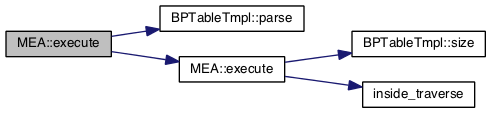
\includegraphics[width=350pt]{namespace_m_e_a_ac823e44d792ae66236b84a5d661236a5_cgraph}
\end{center}
\end{figure}


\hypertarget{namespace_m_e_a_ac4c2f8f5f874e59fa6137637247cb535}{\index{M\+E\+A@{M\+E\+A}!execute@{execute}}
\index{execute@{execute}!M\+E\+A@{M\+E\+A}}
\subsubsection[{execute}]{\setlength{\rightskip}{0pt plus 5cm}template$<$class V $>$ V M\+E\+A\+::execute (
\begin{DoxyParamCaption}
\item[{const {\bf B\+P\+Table\+Tmpl}$<$ V $>$ \&}]{bp, }
\item[{std\+::string \&}]{paren, }
\item[{float}]{gamma}
\end{DoxyParamCaption}
)}}\label{namespace_m_e_a_ac4c2f8f5f874e59fa6137637247cb535}


Definition at line 159 of file mea.\+cpp.



Here is the call graph for this function\+:
\nopagebreak
\begin{figure}[H]
\begin{center}
\leavevmode
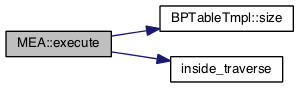
\includegraphics[width=296pt]{namespace_m_e_a_ac4c2f8f5f874e59fa6137637247cb535_cgraph}
\end{center}
\end{figure}




Here is the caller graph for this function\+:
\nopagebreak
\begin{figure}[H]
\begin{center}
\leavevmode
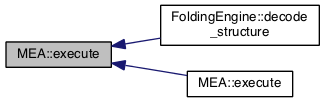
\includegraphics[width=316pt]{namespace_m_e_a_ac4c2f8f5f874e59fa6137637247cb535_icgraph}
\end{center}
\end{figure}


\hypertarget{namespace_m_e_a_ae7da3a697d03f2697f3822dad28ae3d7}{\index{M\+E\+A@{M\+E\+A}!execute@{execute}}
\index{execute@{execute}!M\+E\+A@{M\+E\+A}}
\subsubsection[{execute}]{\setlength{\rightskip}{0pt plus 5cm}template$<$class V $>$ V M\+E\+A\+::execute (
\begin{DoxyParamCaption}
\item[{const {\bf B\+P\+Table\+Tmpl}$<$ V $>$ \&}]{bp, }
\item[{std\+::string \&}]{paren, }
\item[{{\bf uint}}]{max\+\_\+dist, }
\item[{float}]{gamma}
\end{DoxyParamCaption}
)}}\label{namespace_m_e_a_ae7da3a697d03f2697f3822dad28ae3d7}


Definition at line 177 of file mea.\+cpp.



Here is the call graph for this function\+:
\nopagebreak
\begin{figure}[H]
\begin{center}
\leavevmode
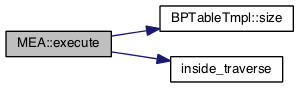
\includegraphics[width=296pt]{namespace_m_e_a_ae7da3a697d03f2697f3822dad28ae3d7_cgraph}
\end{center}
\end{figure}



\hypertarget{namespace_p_r_o_b_c_o_n_s}{\section{P\+R\+O\+B\+C\+O\+N\+S Namespace Reference}
\label{namespace_p_r_o_b_c_o_n_s}\index{P\+R\+O\+B\+C\+O\+N\+S@{P\+R\+O\+B\+C\+O\+N\+S}}
}
\subsection*{Classes}
\begin{DoxyCompactItemize}
\item 
class \hyperlink{class_p_r_o_b_c_o_n_s_1_1_file_buffer}{File\+Buffer}
\item 
class \hyperlink{class_p_r_o_b_c_o_n_s_1_1_multi_sequence}{Multi\+Sequence}
\item 
class \hyperlink{class_p_r_o_b_c_o_n_s_1_1_probabilistic_model}{Probabilistic\+Model}
\item 
class \hyperlink{class_p_r_o_b_c_o_n_s_1_1_probcons}{Probcons}
\item 
class \hyperlink{class_p_r_o_b_c_o_n_s_1_1_safe_vector}{Safe\+Vector}
\item 
class \hyperlink{class_p_r_o_b_c_o_n_s_1_1_sequence}{Sequence}
\item 
class \hyperlink{class_p_r_o_b_c_o_n_s_1_1_sparse_matrix}{Sparse\+Matrix}
\end{DoxyCompactItemize}
\subsection*{Typedefs}
\begin{DoxyCompactItemize}
\item 
typedef \hyperlink{class_p_r_o_b_c_o_n_s_1_1_safe_vector}{Safe\+Vector}$<$ int $>$ \hyperlink{namespace_p_r_o_b_c_o_n_s_af5836390f1b6599e5a0337a7dcd4b5d7}{V\+I}
\item 
typedef \hyperlink{class_p_r_o_b_c_o_n_s_1_1_safe_vector}{Safe\+Vector}$<$ \hyperlink{namespace_p_r_o_b_c_o_n_s_af5836390f1b6599e5a0337a7dcd4b5d7}{V\+I} $>$ \hyperlink{namespace_p_r_o_b_c_o_n_s_a641706f2197f8a5569b46b7ab218a477}{V\+V\+I}
\item 
typedef \hyperlink{class_p_r_o_b_c_o_n_s_1_1_safe_vector}{Safe\+Vector}$<$ \hyperlink{namespace_p_r_o_b_c_o_n_s_a641706f2197f8a5569b46b7ab218a477}{V\+V\+I} $>$ \hyperlink{namespace_p_r_o_b_c_o_n_s_a503407de78ebd65ad6c605841c125622}{V\+V\+V\+I}
\item 
typedef \hyperlink{class_p_r_o_b_c_o_n_s_1_1_safe_vector}{Safe\+Vector}$<$ float $>$ \hyperlink{namespace_p_r_o_b_c_o_n_s_a7d46b91dfef3fa4038545a492ad12221}{V\+F}
\item 
typedef \hyperlink{class_p_r_o_b_c_o_n_s_1_1_safe_vector}{Safe\+Vector}$<$ \hyperlink{namespace_p_r_o_b_c_o_n_s_a7d46b91dfef3fa4038545a492ad12221}{V\+F} $>$ \hyperlink{namespace_p_r_o_b_c_o_n_s_a64c77882f700f0f6e9426241c7d7ba1c}{V\+V\+F}
\item 
typedef \hyperlink{class_p_r_o_b_c_o_n_s_1_1_safe_vector}{Safe\+Vector}$<$ \hyperlink{namespace_p_r_o_b_c_o_n_s_a64c77882f700f0f6e9426241c7d7ba1c}{V\+V\+F} $>$ \hyperlink{namespace_p_r_o_b_c_o_n_s_a52a210cf4dfe0ea3c7d83898230cfeaf}{V\+V\+V\+F}
\item 
typedef float \hyperlink{namespace_p_r_o_b_c_o_n_s_a93b8c2a0a0de0dd3d36b847946ed288c}{Score\+Type}
\item 
typedef pair$<$ int, float $>$ \hyperlink{namespace_p_r_o_b_c_o_n_s_a397767dfc075ae6ba7e480f5f06edc32}{P\+I\+F}
\end{DoxyCompactItemize}
\subsection*{Functions}
\begin{DoxyCompactItemize}
\item 
\hyperlink{namespace_p_r_o_b_c_o_n_s_a93b8c2a0a0de0dd3d36b847946ed288c}{Score\+Type} \hyperlink{namespace_p_r_o_b_c_o_n_s_a67887e64b5e38dd2e82ae6db364b1d0d}{L\+O\+G} (\hyperlink{namespace_p_r_o_b_c_o_n_s_a93b8c2a0a0de0dd3d36b847946ed288c}{Score\+Type} x)
\item 
\hyperlink{namespace_p_r_o_b_c_o_n_s_a93b8c2a0a0de0dd3d36b847946ed288c}{Score\+Type} \hyperlink{namespace_p_r_o_b_c_o_n_s_aa7e1016a9ee998c345adada8e2d1659e}{E\+X\+P} (\hyperlink{namespace_p_r_o_b_c_o_n_s_a93b8c2a0a0de0dd3d36b847946ed288c}{Score\+Type} x)
\item 
float \hyperlink{namespace_p_r_o_b_c_o_n_s_a5b24ca83fd4ec95bdcce003fcf66700a}{L\+O\+O\+K\+U\+P} (float x)
\item 
float \hyperlink{namespace_p_r_o_b_c_o_n_s_a2744e5b759674efe2c2eec891813eb31}{L\+O\+O\+K\+U\+P\+\_\+\+S\+L\+O\+W} (float x)
\item 
float \hyperlink{namespace_p_r_o_b_c_o_n_s_ad6d22c04d26dd86d1a6fd3a3d7cd00ae}{M\+A\+X} (float x, float y, float z)
\item 
void \hyperlink{namespace_p_r_o_b_c_o_n_s_a42a70b7737376d14938ac0135863deb1}{L\+O\+G\+\_\+\+P\+L\+U\+S\+\_\+\+E\+Q\+U\+A\+L\+S} (float \&x, float y)
\item 
void \hyperlink{namespace_p_r_o_b_c_o_n_s_ad87c394a7040cf7ab9ab7038db967ecb}{L\+O\+G\+\_\+\+P\+L\+U\+S\+\_\+\+E\+Q\+U\+A\+L\+S\+\_\+\+S\+L\+O\+W} (float \&x, float y)
\item 
float \hyperlink{namespace_p_r_o_b_c_o_n_s_a45d2b07d0c918cef2ebc0f5d116e443e}{L\+O\+G\+\_\+\+A\+D\+D} (float x, float y)
\item 
float \hyperlink{namespace_p_r_o_b_c_o_n_s_a20d1a1990fc2a2eb3d7af919324d453c}{L\+O\+G\+\_\+\+A\+D\+D} (float x1, float x2, float x3)
\item 
float \hyperlink{namespace_p_r_o_b_c_o_n_s_ae97e1e684a07d63e65e3f2ca7155c148}{L\+O\+G\+\_\+\+A\+D\+D} (float x1, float x2, float x3, float x4)
\item 
float \hyperlink{namespace_p_r_o_b_c_o_n_s_a3ce8799c3d24d8fd1a78b7dd0a5335bf}{L\+O\+G\+\_\+\+A\+D\+D} (float x1, float x2, float x3, float x4, float x5)
\item 
float \hyperlink{namespace_p_r_o_b_c_o_n_s_aae5d50407b95bc0f72cdeb413e2e4fdd}{L\+O\+G\+\_\+\+A\+D\+D} (float x1, float x2, float x3, float x4, float x5, float x6)
\item 
float \hyperlink{namespace_p_r_o_b_c_o_n_s_abc231304d5d131d26c635ee7121f3619}{L\+O\+G\+\_\+\+A\+D\+D} (float x1, float x2, float x3, float x4, float x5, float x6, float x7)
\item 
void \hyperlink{namespace_p_r_o_b_c_o_n_s_a40f96f04d0cecca659a9585ded4975b0}{Choose\+Best\+Of\+Three} (float x1, float x2, float x3, char b1, char b2, char b3, float $\ast$x, char $\ast$b)
\item 
\hyperlink{namespace_p_r_o_b_c_o_n_s_a7d46b91dfef3fa4038545a492ad12221}{V\+F} \hyperlink{namespace_p_r_o_b_c_o_n_s_aad90cbdf21742e0d50a23be886afbffe}{gap\+Open} (2 $\ast$Num\+Insert\+States)
\item 
\hyperlink{namespace_p_r_o_b_c_o_n_s_a7d46b91dfef3fa4038545a492ad12221}{V\+F} \hyperlink{namespace_p_r_o_b_c_o_n_s_ae1d3cf6541679992bb3dc1a89e0347d5}{gap\+Extend} (2 $\ast$Num\+Insert\+States)
\end{DoxyCompactItemize}
\subsection*{Variables}
\begin{DoxyCompactItemize}
\item 
float \hyperlink{namespace_p_r_o_b_c_o_n_s_aa8038b03680de2e2d9a1887d20b5467f}{init\+Distrib1\+Default} \mbox{[}$\,$\mbox{]} = \{ 0.\+9588437676f, 0.\+0205782652f, 0.\+0205782652f \}
\item 
float \hyperlink{namespace_p_r_o_b_c_o_n_s_a5b6da1afa90c7279231be6813ac26c37}{gap\+Open1\+Default} \mbox{[}$\,$\mbox{]} = \{ 0.\+0190259293f, 0.\+0190259293f \}
\item 
float \hyperlink{namespace_p_r_o_b_c_o_n_s_a833e6c5dcb9594b964de8651c139d655}{gap\+Extend1\+Default} \mbox{[}$\,$\mbox{]} = \{ 0.\+3269913495f, 0.\+3269913495f \}
\item 
float \hyperlink{namespace_p_r_o_b_c_o_n_s_a7c5ee053f6a08b12797553be09091fbb}{init\+Distrib2\+Default} \mbox{[}$\,$\mbox{]} = \{ 0.\+9615409374f, 0.\+0000004538f, 0.\+0000004538f, 0.\+0192291681f, 0.\+0192291681f \}
\item 
float \hyperlink{namespace_p_r_o_b_c_o_n_s_a7b3932227ab3389404600ec5c3609d0d}{gap\+Open2\+Default} \mbox{[}$\,$\mbox{]} = \{ 0.\+0082473317f, 0.\+0082473317f, 0.\+0107844425f, 0.\+0107844425f \}
\item 
float \hyperlink{namespace_p_r_o_b_c_o_n_s_a1880db9507d0a694a8858b86c81c91ed}{gap\+Extend2\+Default} \mbox{[}$\,$\mbox{]} = \{ 0.\+3210460842f, 0.\+3210460842f, 0.\+3298229277f, 0.\+3298229277f \}
\item 
string \hyperlink{namespace_p_r_o_b_c_o_n_s_ae29cac54ccf09bf5f57237867b6da88b}{alphabet\+Default} = \char`\"{}A\+C\+G\+U\+T\+N\char`\"{}
\item 
float \hyperlink{namespace_p_r_o_b_c_o_n_s_ae1a79b9f9d56a9e4a4fb4549fbfd8c26}{emit\+Single\+Default} \mbox{[}6\mbox{]}
\item 
float \hyperlink{namespace_p_r_o_b_c_o_n_s_a7b7f8e2ed1d48ae7f4003a455d3f7150}{emit\+Pairs\+Default} \mbox{[}6\mbox{]}\mbox{[}6\mbox{]}
\item 
const int \hyperlink{namespace_p_r_o_b_c_o_n_s_ab9d548ecc7df58e583023207ab844623}{Buffer\+Size} = 1000
\item 
const int \hyperlink{namespace_p_r_o_b_c_o_n_s_a1ce3646341e8ca6190adcf1ae31e1cb6}{Num\+Match\+States} = 1
\item 
const int \hyperlink{namespace_p_r_o_b_c_o_n_s_aa757f46fbcab58d09517a449a680db3b}{Num\+Matrix\+Types} = \hyperlink{namespace_p_r_o_b_c_o_n_s_a1ce3646341e8ca6190adcf1ae31e1cb6}{Num\+Match\+States} + Num\+Insert\+States $\ast$ 2
\item 
const float \hyperlink{namespace_p_r_o_b_c_o_n_s_ae5514101b91c6ae08ed2ee9306d2305d}{L\+O\+G\+\_\+\+Z\+E\+R\+O} = -\/2e20
\item 
const float \hyperlink{namespace_p_r_o_b_c_o_n_s_a5b8b50011bc3908106307aacd3a58d6e}{L\+O\+G\+\_\+\+O\+N\+E} = 0.\+0
\item 
const float \hyperlink{namespace_p_r_o_b_c_o_n_s_a4074cb3928409c0f0b0d7fce9d2576b0}{E\+X\+P\+\_\+\+U\+N\+D\+E\+R\+F\+L\+O\+W\+\_\+\+T\+H\+R\+E\+S\+H\+O\+L\+D} = -\/4.\+6
\item 
const float \hyperlink{namespace_p_r_o_b_c_o_n_s_acbc36709b1c9a80fa2ec8ead6e1a73ee}{L\+O\+G\+\_\+\+U\+N\+D\+E\+R\+F\+L\+O\+W\+\_\+\+T\+H\+R\+E\+S\+H\+O\+L\+D} = 7.\+5
\item 
const float \hyperlink{namespace_p_r_o_b_c_o_n_s_af5a75afbb515bc75473200f8a3ba1993}{P\+O\+S\+T\+E\+R\+I\+O\+R\+\_\+\+C\+U\+T\+O\+F\+F} = 0.\+01
\item 
\hyperlink{namespace_p_r_o_b_c_o_n_s_a7d46b91dfef3fa4038545a492ad12221}{V\+F} \hyperlink{namespace_p_r_o_b_c_o_n_s_a4fa8c099c73924e7f54dc5dbf2377aff}{init\+Distrib} (\hyperlink{namespace_p_r_o_b_c_o_n_s_aa757f46fbcab58d09517a449a680db3b}{Num\+Matrix\+Types})
\item 
\hyperlink{namespace_p_r_o_b_c_o_n_s_a64c77882f700f0f6e9426241c7d7ba1c}{V\+V\+F} \hyperlink{namespace_p_r_o_b_c_o_n_s_ae28575916501eeab36245ba0624d0640}{emit\+Pairs} (256, \hyperlink{namespace_p_r_o_b_c_o_n_s_a7d46b91dfef3fa4038545a492ad12221}{V\+F}(256, 1e-\/10))
\item 
\hyperlink{namespace_p_r_o_b_c_o_n_s_a7d46b91dfef3fa4038545a492ad12221}{V\+F} \hyperlink{namespace_p_r_o_b_c_o_n_s_a60ce52cd8ccb26631e13fecca788f13e}{emit\+Single} (256, 1e-\/5)
\item 
string \hyperlink{namespace_p_r_o_b_c_o_n_s_a1e5ecbd30c93a113dcef4ef53f00d110}{alphabet} = \hyperlink{namespace_p_r_o_b_c_o_n_s_ae29cac54ccf09bf5f57237867b6da88b}{alphabet\+Default}
\end{DoxyCompactItemize}


\subsection{Typedef Documentation}
\hypertarget{namespace_p_r_o_b_c_o_n_s_a397767dfc075ae6ba7e480f5f06edc32}{\index{P\+R\+O\+B\+C\+O\+N\+S@{P\+R\+O\+B\+C\+O\+N\+S}!P\+I\+F@{P\+I\+F}}
\index{P\+I\+F@{P\+I\+F}!P\+R\+O\+B\+C\+O\+N\+S@{P\+R\+O\+B\+C\+O\+N\+S}}
\subsubsection[{P\+I\+F}]{\setlength{\rightskip}{0pt plus 5cm}typedef pair$<$int,float$>$ {\bf P\+R\+O\+B\+C\+O\+N\+S\+::\+P\+I\+F}}}\label{namespace_p_r_o_b_c_o_n_s_a397767dfc075ae6ba7e480f5f06edc32}


Definition at line 20 of file Sparse\+Matrix.\+h.

\hypertarget{namespace_p_r_o_b_c_o_n_s_a93b8c2a0a0de0dd3d36b847946ed288c}{\index{P\+R\+O\+B\+C\+O\+N\+S@{P\+R\+O\+B\+C\+O\+N\+S}!Score\+Type@{Score\+Type}}
\index{Score\+Type@{Score\+Type}!P\+R\+O\+B\+C\+O\+N\+S@{P\+R\+O\+B\+C\+O\+N\+S}}
\subsubsection[{Score\+Type}]{\setlength{\rightskip}{0pt plus 5cm}typedef float {\bf P\+R\+O\+B\+C\+O\+N\+S\+::\+Score\+Type}}}\label{namespace_p_r_o_b_c_o_n_s_a93b8c2a0a0de0dd3d36b847946ed288c}


Definition at line 16 of file Score\+Type.\+h.

\hypertarget{namespace_p_r_o_b_c_o_n_s_a7d46b91dfef3fa4038545a492ad12221}{\index{P\+R\+O\+B\+C\+O\+N\+S@{P\+R\+O\+B\+C\+O\+N\+S}!V\+F@{V\+F}}
\index{V\+F@{V\+F}!P\+R\+O\+B\+C\+O\+N\+S@{P\+R\+O\+B\+C\+O\+N\+S}}
\subsubsection[{V\+F}]{\setlength{\rightskip}{0pt plus 5cm}typedef {\bf Safe\+Vector}$<$float$>$ {\bf P\+R\+O\+B\+C\+O\+N\+S\+::\+V\+F}}}\label{namespace_p_r_o_b_c_o_n_s_a7d46b91dfef3fa4038545a492ad12221}


Definition at line 53 of file Safe\+Vector.\+h.

\hypertarget{namespace_p_r_o_b_c_o_n_s_af5836390f1b6599e5a0337a7dcd4b5d7}{\index{P\+R\+O\+B\+C\+O\+N\+S@{P\+R\+O\+B\+C\+O\+N\+S}!V\+I@{V\+I}}
\index{V\+I@{V\+I}!P\+R\+O\+B\+C\+O\+N\+S@{P\+R\+O\+B\+C\+O\+N\+S}}
\subsubsection[{V\+I}]{\setlength{\rightskip}{0pt plus 5cm}typedef {\bf Safe\+Vector}$<$int$>$ {\bf P\+R\+O\+B\+C\+O\+N\+S\+::\+V\+I}}}\label{namespace_p_r_o_b_c_o_n_s_af5836390f1b6599e5a0337a7dcd4b5d7}


Definition at line 50 of file Safe\+Vector.\+h.

\hypertarget{namespace_p_r_o_b_c_o_n_s_a64c77882f700f0f6e9426241c7d7ba1c}{\index{P\+R\+O\+B\+C\+O\+N\+S@{P\+R\+O\+B\+C\+O\+N\+S}!V\+V\+F@{V\+V\+F}}
\index{V\+V\+F@{V\+V\+F}!P\+R\+O\+B\+C\+O\+N\+S@{P\+R\+O\+B\+C\+O\+N\+S}}
\subsubsection[{V\+V\+F}]{\setlength{\rightskip}{0pt plus 5cm}typedef {\bf Safe\+Vector}$<${\bf V\+F}$>$ {\bf P\+R\+O\+B\+C\+O\+N\+S\+::\+V\+V\+F}}}\label{namespace_p_r_o_b_c_o_n_s_a64c77882f700f0f6e9426241c7d7ba1c}


Definition at line 54 of file Safe\+Vector.\+h.

\hypertarget{namespace_p_r_o_b_c_o_n_s_a641706f2197f8a5569b46b7ab218a477}{\index{P\+R\+O\+B\+C\+O\+N\+S@{P\+R\+O\+B\+C\+O\+N\+S}!V\+V\+I@{V\+V\+I}}
\index{V\+V\+I@{V\+V\+I}!P\+R\+O\+B\+C\+O\+N\+S@{P\+R\+O\+B\+C\+O\+N\+S}}
\subsubsection[{V\+V\+I}]{\setlength{\rightskip}{0pt plus 5cm}typedef {\bf Safe\+Vector}$<${\bf V\+I}$>$ {\bf P\+R\+O\+B\+C\+O\+N\+S\+::\+V\+V\+I}}}\label{namespace_p_r_o_b_c_o_n_s_a641706f2197f8a5569b46b7ab218a477}


Definition at line 51 of file Safe\+Vector.\+h.

\hypertarget{namespace_p_r_o_b_c_o_n_s_a52a210cf4dfe0ea3c7d83898230cfeaf}{\index{P\+R\+O\+B\+C\+O\+N\+S@{P\+R\+O\+B\+C\+O\+N\+S}!V\+V\+V\+F@{V\+V\+V\+F}}
\index{V\+V\+V\+F@{V\+V\+V\+F}!P\+R\+O\+B\+C\+O\+N\+S@{P\+R\+O\+B\+C\+O\+N\+S}}
\subsubsection[{V\+V\+V\+F}]{\setlength{\rightskip}{0pt plus 5cm}typedef {\bf Safe\+Vector}$<${\bf V\+V\+F}$>$ {\bf P\+R\+O\+B\+C\+O\+N\+S\+::\+V\+V\+V\+F}}}\label{namespace_p_r_o_b_c_o_n_s_a52a210cf4dfe0ea3c7d83898230cfeaf}


Definition at line 55 of file Safe\+Vector.\+h.

\hypertarget{namespace_p_r_o_b_c_o_n_s_a503407de78ebd65ad6c605841c125622}{\index{P\+R\+O\+B\+C\+O\+N\+S@{P\+R\+O\+B\+C\+O\+N\+S}!V\+V\+V\+I@{V\+V\+V\+I}}
\index{V\+V\+V\+I@{V\+V\+V\+I}!P\+R\+O\+B\+C\+O\+N\+S@{P\+R\+O\+B\+C\+O\+N\+S}}
\subsubsection[{V\+V\+V\+I}]{\setlength{\rightskip}{0pt plus 5cm}typedef {\bf Safe\+Vector}$<${\bf V\+V\+I}$>$ {\bf P\+R\+O\+B\+C\+O\+N\+S\+::\+V\+V\+V\+I}}}\label{namespace_p_r_o_b_c_o_n_s_a503407de78ebd65ad6c605841c125622}


Definition at line 52 of file Safe\+Vector.\+h.



\subsection{Function Documentation}
\hypertarget{namespace_p_r_o_b_c_o_n_s_a40f96f04d0cecca659a9585ded4975b0}{\index{P\+R\+O\+B\+C\+O\+N\+S@{P\+R\+O\+B\+C\+O\+N\+S}!Choose\+Best\+Of\+Three@{Choose\+Best\+Of\+Three}}
\index{Choose\+Best\+Of\+Three@{Choose\+Best\+Of\+Three}!P\+R\+O\+B\+C\+O\+N\+S@{P\+R\+O\+B\+C\+O\+N\+S}}
\subsubsection[{Choose\+Best\+Of\+Three}]{\setlength{\rightskip}{0pt plus 5cm}void P\+R\+O\+B\+C\+O\+N\+S\+::\+Choose\+Best\+Of\+Three (
\begin{DoxyParamCaption}
\item[{float}]{x1, }
\item[{float}]{x2, }
\item[{float}]{x3, }
\item[{char}]{b1, }
\item[{char}]{b2, }
\item[{char}]{b3, }
\item[{float $\ast$}]{x, }
\item[{char $\ast$}]{b}
\end{DoxyParamCaption}
)\hspace{0.3cm}{\ttfamily [inline]}}}\label{namespace_p_r_o_b_c_o_n_s_a40f96f04d0cecca659a9585ded4975b0}


Definition at line 322 of file Score\+Type.\+h.



Here is the caller graph for this function\+:
\nopagebreak
\begin{figure}[H]
\begin{center}
\leavevmode
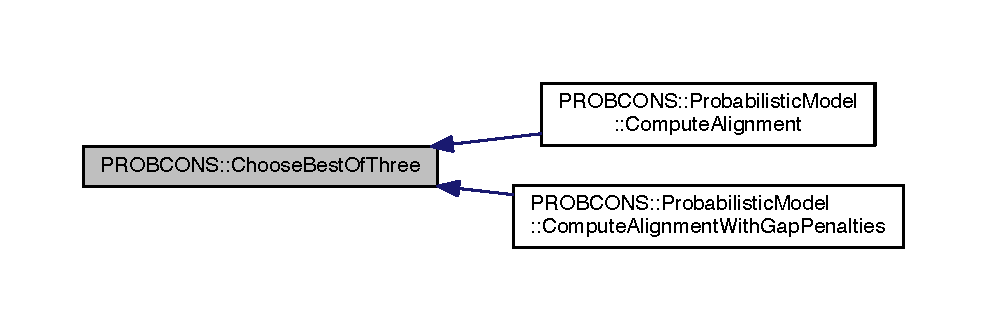
\includegraphics[width=350pt]{namespace_p_r_o_b_c_o_n_s_a40f96f04d0cecca659a9585ded4975b0_icgraph}
\end{center}
\end{figure}


\hypertarget{namespace_p_r_o_b_c_o_n_s_aa7e1016a9ee998c345adada8e2d1659e}{\index{P\+R\+O\+B\+C\+O\+N\+S@{P\+R\+O\+B\+C\+O\+N\+S}!E\+X\+P@{E\+X\+P}}
\index{E\+X\+P@{E\+X\+P}!P\+R\+O\+B\+C\+O\+N\+S@{P\+R\+O\+B\+C\+O\+N\+S}}
\subsubsection[{E\+X\+P}]{\setlength{\rightskip}{0pt plus 5cm}{\bf Score\+Type} P\+R\+O\+B\+C\+O\+N\+S\+::\+E\+X\+P (
\begin{DoxyParamCaption}
\item[{Score\+Type}]{x}
\end{DoxyParamCaption}
)\hspace{0.3cm}{\ttfamily [inline]}}}\label{namespace_p_r_o_b_c_o_n_s_aa7e1016a9ee998c345adada8e2d1659e}


Definition at line 37 of file Score\+Type.\+h.



Here is the caller graph for this function\+:
\nopagebreak
\begin{figure}[H]
\begin{center}
\leavevmode
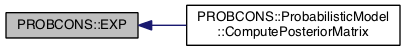
\includegraphics[width=350pt]{namespace_p_r_o_b_c_o_n_s_aa7e1016a9ee998c345adada8e2d1659e_icgraph}
\end{center}
\end{figure}


\hypertarget{namespace_p_r_o_b_c_o_n_s_ae1d3cf6541679992bb3dc1a89e0347d5}{\index{P\+R\+O\+B\+C\+O\+N\+S@{P\+R\+O\+B\+C\+O\+N\+S}!gap\+Extend@{gap\+Extend}}
\index{gap\+Extend@{gap\+Extend}!P\+R\+O\+B\+C\+O\+N\+S@{P\+R\+O\+B\+C\+O\+N\+S}}
\subsubsection[{gap\+Extend}]{\setlength{\rightskip}{0pt plus 5cm}{\bf V\+F} P\+R\+O\+B\+C\+O\+N\+S\+::gap\+Extend (
\begin{DoxyParamCaption}
\item[{2 $\ast$}]{Num\+Insert\+States}
\end{DoxyParamCaption}
)}}\label{namespace_p_r_o_b_c_o_n_s_ae1d3cf6541679992bb3dc1a89e0347d5}


Here is the caller graph for this function\+:
\nopagebreak
\begin{figure}[H]
\begin{center}
\leavevmode
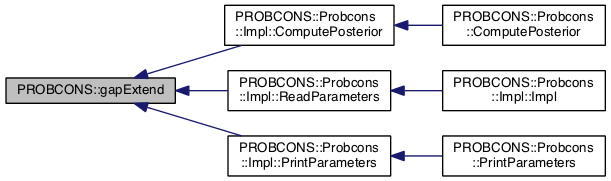
\includegraphics[width=350pt]{namespace_p_r_o_b_c_o_n_s_ae1d3cf6541679992bb3dc1a89e0347d5_icgraph}
\end{center}
\end{figure}


\hypertarget{namespace_p_r_o_b_c_o_n_s_aad90cbdf21742e0d50a23be886afbffe}{\index{P\+R\+O\+B\+C\+O\+N\+S@{P\+R\+O\+B\+C\+O\+N\+S}!gap\+Open@{gap\+Open}}
\index{gap\+Open@{gap\+Open}!P\+R\+O\+B\+C\+O\+N\+S@{P\+R\+O\+B\+C\+O\+N\+S}}
\subsubsection[{gap\+Open}]{\setlength{\rightskip}{0pt plus 5cm}{\bf V\+F} P\+R\+O\+B\+C\+O\+N\+S\+::gap\+Open (
\begin{DoxyParamCaption}
\item[{2 $\ast$}]{Num\+Insert\+States}
\end{DoxyParamCaption}
)}}\label{namespace_p_r_o_b_c_o_n_s_aad90cbdf21742e0d50a23be886afbffe}


Here is the caller graph for this function\+:
\nopagebreak
\begin{figure}[H]
\begin{center}
\leavevmode
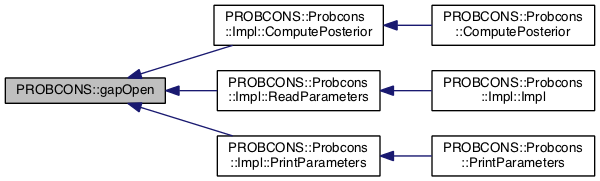
\includegraphics[width=350pt]{namespace_p_r_o_b_c_o_n_s_aad90cbdf21742e0d50a23be886afbffe_icgraph}
\end{center}
\end{figure}


\hypertarget{namespace_p_r_o_b_c_o_n_s_a67887e64b5e38dd2e82ae6db364b1d0d}{\index{P\+R\+O\+B\+C\+O\+N\+S@{P\+R\+O\+B\+C\+O\+N\+S}!L\+O\+G@{L\+O\+G}}
\index{L\+O\+G@{L\+O\+G}!P\+R\+O\+B\+C\+O\+N\+S@{P\+R\+O\+B\+C\+O\+N\+S}}
\subsubsection[{L\+O\+G}]{\setlength{\rightskip}{0pt plus 5cm}{\bf Score\+Type} P\+R\+O\+B\+C\+O\+N\+S\+::\+L\+O\+G (
\begin{DoxyParamCaption}
\item[{Score\+Type}]{x}
\end{DoxyParamCaption}
)\hspace{0.3cm}{\ttfamily [inline]}}}\label{namespace_p_r_o_b_c_o_n_s_a67887e64b5e38dd2e82ae6db364b1d0d}


Definition at line 27 of file Score\+Type.\+h.



Here is the caller graph for this function\+:
\nopagebreak
\begin{figure}[H]
\begin{center}
\leavevmode
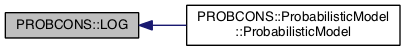
\includegraphics[width=350pt]{namespace_p_r_o_b_c_o_n_s_a67887e64b5e38dd2e82ae6db364b1d0d_icgraph}
\end{center}
\end{figure}


\hypertarget{namespace_p_r_o_b_c_o_n_s_a45d2b07d0c918cef2ebc0f5d116e443e}{\index{P\+R\+O\+B\+C\+O\+N\+S@{P\+R\+O\+B\+C\+O\+N\+S}!L\+O\+G\+\_\+\+A\+D\+D@{L\+O\+G\+\_\+\+A\+D\+D}}
\index{L\+O\+G\+\_\+\+A\+D\+D@{L\+O\+G\+\_\+\+A\+D\+D}!P\+R\+O\+B\+C\+O\+N\+S@{P\+R\+O\+B\+C\+O\+N\+S}}
\subsubsection[{L\+O\+G\+\_\+\+A\+D\+D}]{\setlength{\rightskip}{0pt plus 5cm}float P\+R\+O\+B\+C\+O\+N\+S\+::\+L\+O\+G\+\_\+\+A\+D\+D (
\begin{DoxyParamCaption}
\item[{float}]{x, }
\item[{float}]{y}
\end{DoxyParamCaption}
)\hspace{0.3cm}{\ttfamily [inline]}}}\label{namespace_p_r_o_b_c_o_n_s_a45d2b07d0c918cef2ebc0f5d116e443e}


Definition at line 259 of file Score\+Type.\+h.



Here is the call graph for this function\+:
\nopagebreak
\begin{figure}[H]
\begin{center}
\leavevmode
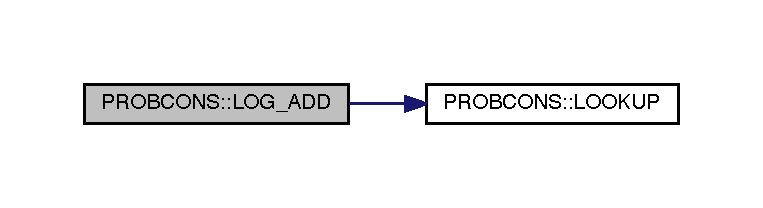
\includegraphics[width=350pt]{namespace_p_r_o_b_c_o_n_s_a45d2b07d0c918cef2ebc0f5d116e443e_cgraph}
\end{center}
\end{figure}




Here is the caller graph for this function\+:
\nopagebreak
\begin{figure}[H]
\begin{center}
\leavevmode
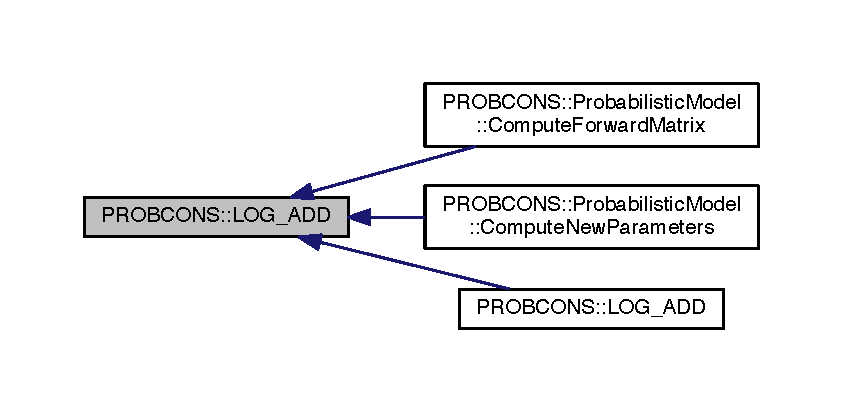
\includegraphics[width=350pt]{namespace_p_r_o_b_c_o_n_s_a45d2b07d0c918cef2ebc0f5d116e443e_icgraph}
\end{center}
\end{figure}


\hypertarget{namespace_p_r_o_b_c_o_n_s_a20d1a1990fc2a2eb3d7af919324d453c}{\index{P\+R\+O\+B\+C\+O\+N\+S@{P\+R\+O\+B\+C\+O\+N\+S}!L\+O\+G\+\_\+\+A\+D\+D@{L\+O\+G\+\_\+\+A\+D\+D}}
\index{L\+O\+G\+\_\+\+A\+D\+D@{L\+O\+G\+\_\+\+A\+D\+D}!P\+R\+O\+B\+C\+O\+N\+S@{P\+R\+O\+B\+C\+O\+N\+S}}
\subsubsection[{L\+O\+G\+\_\+\+A\+D\+D}]{\setlength{\rightskip}{0pt plus 5cm}float P\+R\+O\+B\+C\+O\+N\+S\+::\+L\+O\+G\+\_\+\+A\+D\+D (
\begin{DoxyParamCaption}
\item[{float}]{x1, }
\item[{float}]{x2, }
\item[{float}]{x3}
\end{DoxyParamCaption}
)\hspace{0.3cm}{\ttfamily [inline]}}}\label{namespace_p_r_o_b_c_o_n_s_a20d1a1990fc2a2eb3d7af919324d453c}


Definition at line 271 of file Score\+Type.\+h.



Here is the call graph for this function\+:
\nopagebreak
\begin{figure}[H]
\begin{center}
\leavevmode
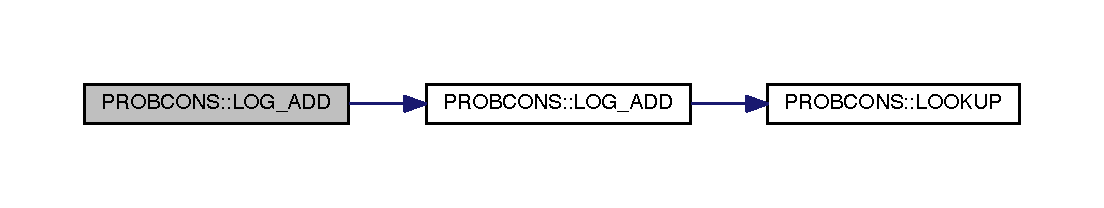
\includegraphics[width=350pt]{namespace_p_r_o_b_c_o_n_s_a20d1a1990fc2a2eb3d7af919324d453c_cgraph}
\end{center}
\end{figure}


\hypertarget{namespace_p_r_o_b_c_o_n_s_ae97e1e684a07d63e65e3f2ca7155c148}{\index{P\+R\+O\+B\+C\+O\+N\+S@{P\+R\+O\+B\+C\+O\+N\+S}!L\+O\+G\+\_\+\+A\+D\+D@{L\+O\+G\+\_\+\+A\+D\+D}}
\index{L\+O\+G\+\_\+\+A\+D\+D@{L\+O\+G\+\_\+\+A\+D\+D}!P\+R\+O\+B\+C\+O\+N\+S@{P\+R\+O\+B\+C\+O\+N\+S}}
\subsubsection[{L\+O\+G\+\_\+\+A\+D\+D}]{\setlength{\rightskip}{0pt plus 5cm}float P\+R\+O\+B\+C\+O\+N\+S\+::\+L\+O\+G\+\_\+\+A\+D\+D (
\begin{DoxyParamCaption}
\item[{float}]{x1, }
\item[{float}]{x2, }
\item[{float}]{x3, }
\item[{float}]{x4}
\end{DoxyParamCaption}
)\hspace{0.3cm}{\ttfamily [inline]}}}\label{namespace_p_r_o_b_c_o_n_s_ae97e1e684a07d63e65e3f2ca7155c148}


Definition at line 281 of file Score\+Type.\+h.



Here is the call graph for this function\+:
\nopagebreak
\begin{figure}[H]
\begin{center}
\leavevmode
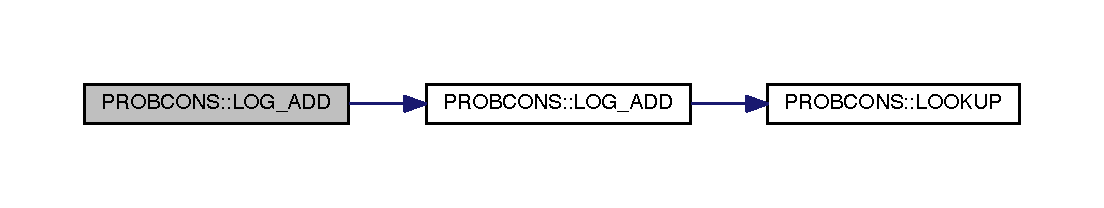
\includegraphics[width=350pt]{namespace_p_r_o_b_c_o_n_s_ae97e1e684a07d63e65e3f2ca7155c148_cgraph}
\end{center}
\end{figure}


\hypertarget{namespace_p_r_o_b_c_o_n_s_a3ce8799c3d24d8fd1a78b7dd0a5335bf}{\index{P\+R\+O\+B\+C\+O\+N\+S@{P\+R\+O\+B\+C\+O\+N\+S}!L\+O\+G\+\_\+\+A\+D\+D@{L\+O\+G\+\_\+\+A\+D\+D}}
\index{L\+O\+G\+\_\+\+A\+D\+D@{L\+O\+G\+\_\+\+A\+D\+D}!P\+R\+O\+B\+C\+O\+N\+S@{P\+R\+O\+B\+C\+O\+N\+S}}
\subsubsection[{L\+O\+G\+\_\+\+A\+D\+D}]{\setlength{\rightskip}{0pt plus 5cm}float P\+R\+O\+B\+C\+O\+N\+S\+::\+L\+O\+G\+\_\+\+A\+D\+D (
\begin{DoxyParamCaption}
\item[{float}]{x1, }
\item[{float}]{x2, }
\item[{float}]{x3, }
\item[{float}]{x4, }
\item[{float}]{x5}
\end{DoxyParamCaption}
)\hspace{0.3cm}{\ttfamily [inline]}}}\label{namespace_p_r_o_b_c_o_n_s_a3ce8799c3d24d8fd1a78b7dd0a5335bf}


Definition at line 291 of file Score\+Type.\+h.



Here is the call graph for this function\+:
\nopagebreak
\begin{figure}[H]
\begin{center}
\leavevmode
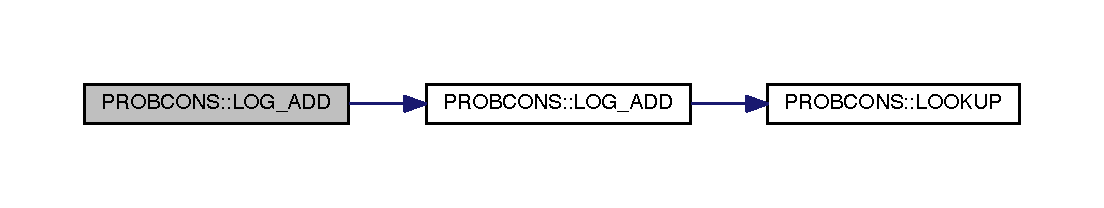
\includegraphics[width=350pt]{namespace_p_r_o_b_c_o_n_s_a3ce8799c3d24d8fd1a78b7dd0a5335bf_cgraph}
\end{center}
\end{figure}


\hypertarget{namespace_p_r_o_b_c_o_n_s_aae5d50407b95bc0f72cdeb413e2e4fdd}{\index{P\+R\+O\+B\+C\+O\+N\+S@{P\+R\+O\+B\+C\+O\+N\+S}!L\+O\+G\+\_\+\+A\+D\+D@{L\+O\+G\+\_\+\+A\+D\+D}}
\index{L\+O\+G\+\_\+\+A\+D\+D@{L\+O\+G\+\_\+\+A\+D\+D}!P\+R\+O\+B\+C\+O\+N\+S@{P\+R\+O\+B\+C\+O\+N\+S}}
\subsubsection[{L\+O\+G\+\_\+\+A\+D\+D}]{\setlength{\rightskip}{0pt plus 5cm}float P\+R\+O\+B\+C\+O\+N\+S\+::\+L\+O\+G\+\_\+\+A\+D\+D (
\begin{DoxyParamCaption}
\item[{float}]{x1, }
\item[{float}]{x2, }
\item[{float}]{x3, }
\item[{float}]{x4, }
\item[{float}]{x5, }
\item[{float}]{x6}
\end{DoxyParamCaption}
)\hspace{0.3cm}{\ttfamily [inline]}}}\label{namespace_p_r_o_b_c_o_n_s_aae5d50407b95bc0f72cdeb413e2e4fdd}


Definition at line 301 of file Score\+Type.\+h.



Here is the call graph for this function\+:
\nopagebreak
\begin{figure}[H]
\begin{center}
\leavevmode
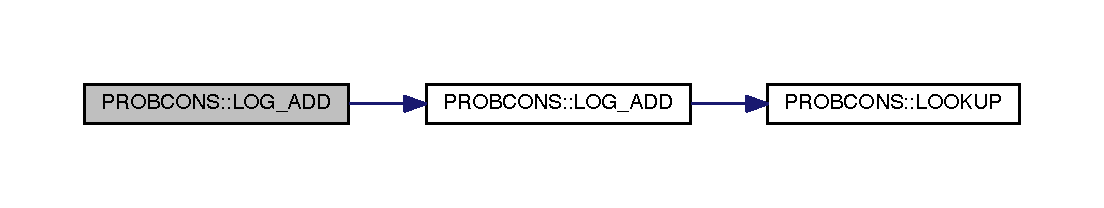
\includegraphics[width=350pt]{namespace_p_r_o_b_c_o_n_s_aae5d50407b95bc0f72cdeb413e2e4fdd_cgraph}
\end{center}
\end{figure}


\hypertarget{namespace_p_r_o_b_c_o_n_s_abc231304d5d131d26c635ee7121f3619}{\index{P\+R\+O\+B\+C\+O\+N\+S@{P\+R\+O\+B\+C\+O\+N\+S}!L\+O\+G\+\_\+\+A\+D\+D@{L\+O\+G\+\_\+\+A\+D\+D}}
\index{L\+O\+G\+\_\+\+A\+D\+D@{L\+O\+G\+\_\+\+A\+D\+D}!P\+R\+O\+B\+C\+O\+N\+S@{P\+R\+O\+B\+C\+O\+N\+S}}
\subsubsection[{L\+O\+G\+\_\+\+A\+D\+D}]{\setlength{\rightskip}{0pt plus 5cm}float P\+R\+O\+B\+C\+O\+N\+S\+::\+L\+O\+G\+\_\+\+A\+D\+D (
\begin{DoxyParamCaption}
\item[{float}]{x1, }
\item[{float}]{x2, }
\item[{float}]{x3, }
\item[{float}]{x4, }
\item[{float}]{x5, }
\item[{float}]{x6, }
\item[{float}]{x7}
\end{DoxyParamCaption}
)\hspace{0.3cm}{\ttfamily [inline]}}}\label{namespace_p_r_o_b_c_o_n_s_abc231304d5d131d26c635ee7121f3619}


Definition at line 311 of file Score\+Type.\+h.



Here is the call graph for this function\+:
\nopagebreak
\begin{figure}[H]
\begin{center}
\leavevmode
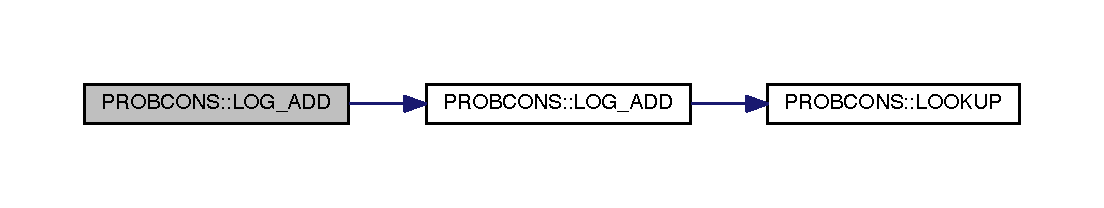
\includegraphics[width=350pt]{namespace_p_r_o_b_c_o_n_s_abc231304d5d131d26c635ee7121f3619_cgraph}
\end{center}
\end{figure}


\hypertarget{namespace_p_r_o_b_c_o_n_s_a42a70b7737376d14938ac0135863deb1}{\index{P\+R\+O\+B\+C\+O\+N\+S@{P\+R\+O\+B\+C\+O\+N\+S}!L\+O\+G\+\_\+\+P\+L\+U\+S\+\_\+\+E\+Q\+U\+A\+L\+S@{L\+O\+G\+\_\+\+P\+L\+U\+S\+\_\+\+E\+Q\+U\+A\+L\+S}}
\index{L\+O\+G\+\_\+\+P\+L\+U\+S\+\_\+\+E\+Q\+U\+A\+L\+S@{L\+O\+G\+\_\+\+P\+L\+U\+S\+\_\+\+E\+Q\+U\+A\+L\+S}!P\+R\+O\+B\+C\+O\+N\+S@{P\+R\+O\+B\+C\+O\+N\+S}}
\subsubsection[{L\+O\+G\+\_\+\+P\+L\+U\+S\+\_\+\+E\+Q\+U\+A\+L\+S}]{\setlength{\rightskip}{0pt plus 5cm}void P\+R\+O\+B\+C\+O\+N\+S\+::\+L\+O\+G\+\_\+\+P\+L\+U\+S\+\_\+\+E\+Q\+U\+A\+L\+S (
\begin{DoxyParamCaption}
\item[{float \&}]{x, }
\item[{float}]{y}
\end{DoxyParamCaption}
)\hspace{0.3cm}{\ttfamily [inline]}}}\label{namespace_p_r_o_b_c_o_n_s_a42a70b7737376d14938ac0135863deb1}


Definition at line 233 of file Score\+Type.\+h.



Here is the call graph for this function\+:
\nopagebreak
\begin{figure}[H]
\begin{center}
\leavevmode
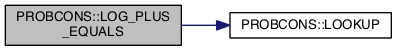
\includegraphics[width=350pt]{namespace_p_r_o_b_c_o_n_s_a42a70b7737376d14938ac0135863deb1_cgraph}
\end{center}
\end{figure}




Here is the caller graph for this function\+:
\nopagebreak
\begin{figure}[H]
\begin{center}
\leavevmode
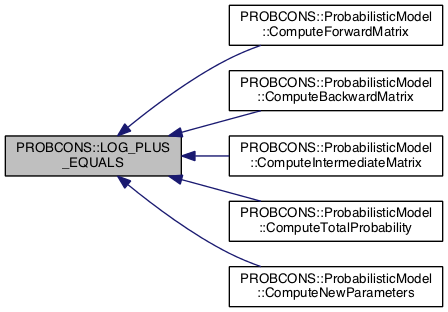
\includegraphics[width=350pt]{namespace_p_r_o_b_c_o_n_s_a42a70b7737376d14938ac0135863deb1_icgraph}
\end{center}
\end{figure}


\hypertarget{namespace_p_r_o_b_c_o_n_s_ad87c394a7040cf7ab9ab7038db967ecb}{\index{P\+R\+O\+B\+C\+O\+N\+S@{P\+R\+O\+B\+C\+O\+N\+S}!L\+O\+G\+\_\+\+P\+L\+U\+S\+\_\+\+E\+Q\+U\+A\+L\+S\+\_\+\+S\+L\+O\+W@{L\+O\+G\+\_\+\+P\+L\+U\+S\+\_\+\+E\+Q\+U\+A\+L\+S\+\_\+\+S\+L\+O\+W}}
\index{L\+O\+G\+\_\+\+P\+L\+U\+S\+\_\+\+E\+Q\+U\+A\+L\+S\+\_\+\+S\+L\+O\+W@{L\+O\+G\+\_\+\+P\+L\+U\+S\+\_\+\+E\+Q\+U\+A\+L\+S\+\_\+\+S\+L\+O\+W}!P\+R\+O\+B\+C\+O\+N\+S@{P\+R\+O\+B\+C\+O\+N\+S}}
\subsubsection[{L\+O\+G\+\_\+\+P\+L\+U\+S\+\_\+\+E\+Q\+U\+A\+L\+S\+\_\+\+S\+L\+O\+W}]{\setlength{\rightskip}{0pt plus 5cm}void P\+R\+O\+B\+C\+O\+N\+S\+::\+L\+O\+G\+\_\+\+P\+L\+U\+S\+\_\+\+E\+Q\+U\+A\+L\+S\+\_\+\+S\+L\+O\+W (
\begin{DoxyParamCaption}
\item[{float \&}]{x, }
\item[{float}]{y}
\end{DoxyParamCaption}
)\hspace{0.3cm}{\ttfamily [inline]}}}\label{namespace_p_r_o_b_c_o_n_s_ad87c394a7040cf7ab9ab7038db967ecb}


Definition at line 246 of file Score\+Type.\+h.



Here is the call graph for this function\+:
\nopagebreak
\begin{figure}[H]
\begin{center}
\leavevmode
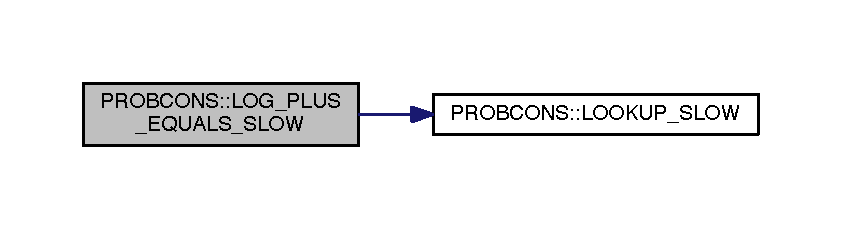
\includegraphics[width=350pt]{namespace_p_r_o_b_c_o_n_s_ad87c394a7040cf7ab9ab7038db967ecb_cgraph}
\end{center}
\end{figure}


\hypertarget{namespace_p_r_o_b_c_o_n_s_a5b24ca83fd4ec95bdcce003fcf66700a}{\index{P\+R\+O\+B\+C\+O\+N\+S@{P\+R\+O\+B\+C\+O\+N\+S}!L\+O\+O\+K\+U\+P@{L\+O\+O\+K\+U\+P}}
\index{L\+O\+O\+K\+U\+P@{L\+O\+O\+K\+U\+P}!P\+R\+O\+B\+C\+O\+N\+S@{P\+R\+O\+B\+C\+O\+N\+S}}
\subsubsection[{L\+O\+O\+K\+U\+P}]{\setlength{\rightskip}{0pt plus 5cm}float P\+R\+O\+B\+C\+O\+N\+S\+::\+L\+O\+O\+K\+U\+P (
\begin{DoxyParamCaption}
\item[{float}]{x}
\end{DoxyParamCaption}
)\hspace{0.3cm}{\ttfamily [inline]}}}\label{namespace_p_r_o_b_c_o_n_s_a5b24ca83fd4ec95bdcce003fcf66700a}


Definition at line 187 of file Score\+Type.\+h.



Here is the caller graph for this function\+:
\nopagebreak
\begin{figure}[H]
\begin{center}
\leavevmode
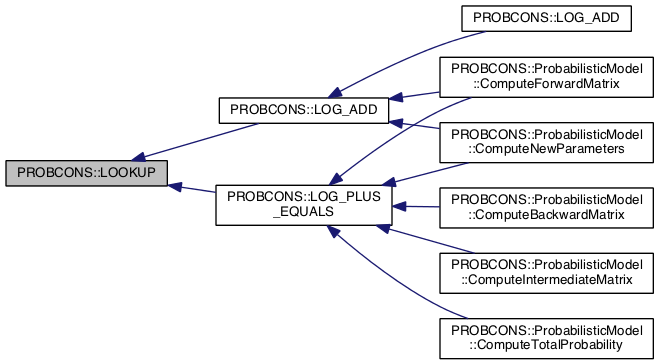
\includegraphics[width=350pt]{namespace_p_r_o_b_c_o_n_s_a5b24ca83fd4ec95bdcce003fcf66700a_icgraph}
\end{center}
\end{figure}


\hypertarget{namespace_p_r_o_b_c_o_n_s_a2744e5b759674efe2c2eec891813eb31}{\index{P\+R\+O\+B\+C\+O\+N\+S@{P\+R\+O\+B\+C\+O\+N\+S}!L\+O\+O\+K\+U\+P\+\_\+\+S\+L\+O\+W@{L\+O\+O\+K\+U\+P\+\_\+\+S\+L\+O\+W}}
\index{L\+O\+O\+K\+U\+P\+\_\+\+S\+L\+O\+W@{L\+O\+O\+K\+U\+P\+\_\+\+S\+L\+O\+W}!P\+R\+O\+B\+C\+O\+N\+S@{P\+R\+O\+B\+C\+O\+N\+S}}
\subsubsection[{L\+O\+O\+K\+U\+P\+\_\+\+S\+L\+O\+W}]{\setlength{\rightskip}{0pt plus 5cm}float P\+R\+O\+B\+C\+O\+N\+S\+::\+L\+O\+O\+K\+U\+P\+\_\+\+S\+L\+O\+W (
\begin{DoxyParamCaption}
\item[{float}]{x}
\end{DoxyParamCaption}
)\hspace{0.3cm}{\ttfamily [inline]}}}\label{namespace_p_r_o_b_c_o_n_s_a2744e5b759674efe2c2eec891813eb31}


Definition at line 206 of file Score\+Type.\+h.



Here is the caller graph for this function\+:
\nopagebreak
\begin{figure}[H]
\begin{center}
\leavevmode
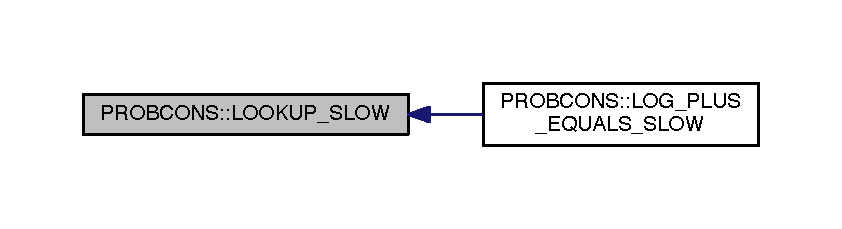
\includegraphics[width=350pt]{namespace_p_r_o_b_c_o_n_s_a2744e5b759674efe2c2eec891813eb31_icgraph}
\end{center}
\end{figure}


\hypertarget{namespace_p_r_o_b_c_o_n_s_ad6d22c04d26dd86d1a6fd3a3d7cd00ae}{\index{P\+R\+O\+B\+C\+O\+N\+S@{P\+R\+O\+B\+C\+O\+N\+S}!M\+A\+X@{M\+A\+X}}
\index{M\+A\+X@{M\+A\+X}!P\+R\+O\+B\+C\+O\+N\+S@{P\+R\+O\+B\+C\+O\+N\+S}}
\subsubsection[{M\+A\+X}]{\setlength{\rightskip}{0pt plus 5cm}float P\+R\+O\+B\+C\+O\+N\+S\+::\+M\+A\+X (
\begin{DoxyParamCaption}
\item[{float}]{x, }
\item[{float}]{y, }
\item[{float}]{z}
\end{DoxyParamCaption}
)\hspace{0.3cm}{\ttfamily [inline]}}}\label{namespace_p_r_o_b_c_o_n_s_ad6d22c04d26dd86d1a6fd3a3d7cd00ae}


Definition at line 216 of file Score\+Type.\+h.



\subsection{Variable Documentation}
\hypertarget{namespace_p_r_o_b_c_o_n_s_a1e5ecbd30c93a113dcef4ef53f00d110}{\index{P\+R\+O\+B\+C\+O\+N\+S@{P\+R\+O\+B\+C\+O\+N\+S}!alphabet@{alphabet}}
\index{alphabet@{alphabet}!P\+R\+O\+B\+C\+O\+N\+S@{P\+R\+O\+B\+C\+O\+N\+S}}
\subsubsection[{alphabet}]{\setlength{\rightskip}{0pt plus 5cm}string P\+R\+O\+B\+C\+O\+N\+S\+::alphabet = {\bf alphabet\+Default}}}\label{namespace_p_r_o_b_c_o_n_s_a1e5ecbd30c93a113dcef4ef53f00d110}


Definition at line 18 of file wrapper.\+cpp.

\hypertarget{namespace_p_r_o_b_c_o_n_s_ae29cac54ccf09bf5f57237867b6da88b}{\index{P\+R\+O\+B\+C\+O\+N\+S@{P\+R\+O\+B\+C\+O\+N\+S}!alphabet\+Default@{alphabet\+Default}}
\index{alphabet\+Default@{alphabet\+Default}!P\+R\+O\+B\+C\+O\+N\+S@{P\+R\+O\+B\+C\+O\+N\+S}}
\subsubsection[{alphabet\+Default}]{\setlength{\rightskip}{0pt plus 5cm}string P\+R\+O\+B\+C\+O\+N\+S\+::alphabet\+Default = \char`\"{}A\+C\+G\+U\+T\+N\char`\"{}}}\label{namespace_p_r_o_b_c_o_n_s_ae29cac54ccf09bf5f57237867b6da88b}


Definition at line 27 of file Defaults.\+h.

\hypertarget{namespace_p_r_o_b_c_o_n_s_ab9d548ecc7df58e583023207ab844623}{\index{P\+R\+O\+B\+C\+O\+N\+S@{P\+R\+O\+B\+C\+O\+N\+S}!Buffer\+Size@{Buffer\+Size}}
\index{Buffer\+Size@{Buffer\+Size}!P\+R\+O\+B\+C\+O\+N\+S@{P\+R\+O\+B\+C\+O\+N\+S}}
\subsubsection[{Buffer\+Size}]{\setlength{\rightskip}{0pt plus 5cm}const int P\+R\+O\+B\+C\+O\+N\+S\+::\+Buffer\+Size = 1000}}\label{namespace_p_r_o_b_c_o_n_s_ab9d548ecc7df58e583023207ab844623}


Definition at line 18 of file File\+Buffer.\+h.

\hypertarget{namespace_p_r_o_b_c_o_n_s_ae28575916501eeab36245ba0624d0640}{\index{P\+R\+O\+B\+C\+O\+N\+S@{P\+R\+O\+B\+C\+O\+N\+S}!emit\+Pairs@{emit\+Pairs}}
\index{emit\+Pairs@{emit\+Pairs}!P\+R\+O\+B\+C\+O\+N\+S@{P\+R\+O\+B\+C\+O\+N\+S}}
\subsubsection[{emit\+Pairs}]{\setlength{\rightskip}{0pt plus 5cm}{\bf V\+V\+F} P\+R\+O\+B\+C\+O\+N\+S\+::emit\+Pairs(256, {\bf V\+F}(256, 1e-\/10))}}\label{namespace_p_r_o_b_c_o_n_s_ae28575916501eeab36245ba0624d0640}
\hypertarget{namespace_p_r_o_b_c_o_n_s_a7b7f8e2ed1d48ae7f4003a455d3f7150}{\index{P\+R\+O\+B\+C\+O\+N\+S@{P\+R\+O\+B\+C\+O\+N\+S}!emit\+Pairs\+Default@{emit\+Pairs\+Default}}
\index{emit\+Pairs\+Default@{emit\+Pairs\+Default}!P\+R\+O\+B\+C\+O\+N\+S@{P\+R\+O\+B\+C\+O\+N\+S}}
\subsubsection[{emit\+Pairs\+Default}]{\setlength{\rightskip}{0pt plus 5cm}float P\+R\+O\+B\+C\+O\+N\+S\+::emit\+Pairs\+Default\mbox{[}6\mbox{]}\mbox{[}6\mbox{]}}}\label{namespace_p_r_o_b_c_o_n_s_a7b7f8e2ed1d48ae7f4003a455d3f7150}
{\bfseries Initial value\+:}
\begin{DoxyCode}
= \{
  \{ 0.1487240046f, 0.0184142999f, 0.0361397006f, 0.0238473993f, 0.0238473993f, 0.0000375308f \},
  \{ 0.0184142999f, 0.1583919972f, 0.0275536999f, 0.0389291011f, 0.0389291011f, 0.0000815823f \},
  \{ 0.0361397006f, 0.0275536999f, 0.1979320049f, 0.0244289003f, 0.0244289003f, 0.0000824765f \},
  \{ 0.0238473993f, 0.0389291011f, 0.0244289003f, 0.1557479948f, 0.1557479948f, 0.0000743985f \},
  \{ 0.0238473993f, 0.0389291011f, 0.0244289003f, 0.1557479948f, 0.1557479948f, 0.0000743985f \},
  \{ 0.0000375308f, 0.0000815823f, 0.0000824765f, 0.0000743985f, 0.0000743985f, 0.0000263252f \}
\}
\end{DoxyCode}


Definition at line 32 of file Defaults.\+h.

\hypertarget{namespace_p_r_o_b_c_o_n_s_a60ce52cd8ccb26631e13fecca788f13e}{\index{P\+R\+O\+B\+C\+O\+N\+S@{P\+R\+O\+B\+C\+O\+N\+S}!emit\+Single@{emit\+Single}}
\index{emit\+Single@{emit\+Single}!P\+R\+O\+B\+C\+O\+N\+S@{P\+R\+O\+B\+C\+O\+N\+S}}
\subsubsection[{emit\+Single}]{\setlength{\rightskip}{0pt plus 5cm}{\bf V\+F} P\+R\+O\+B\+C\+O\+N\+S\+::emit\+Single(256, 1e-\/5)}}\label{namespace_p_r_o_b_c_o_n_s_a60ce52cd8ccb26631e13fecca788f13e}
\hypertarget{namespace_p_r_o_b_c_o_n_s_ae1a79b9f9d56a9e4a4fb4549fbfd8c26}{\index{P\+R\+O\+B\+C\+O\+N\+S@{P\+R\+O\+B\+C\+O\+N\+S}!emit\+Single\+Default@{emit\+Single\+Default}}
\index{emit\+Single\+Default@{emit\+Single\+Default}!P\+R\+O\+B\+C\+O\+N\+S@{P\+R\+O\+B\+C\+O\+N\+S}}
\subsubsection[{emit\+Single\+Default}]{\setlength{\rightskip}{0pt plus 5cm}float P\+R\+O\+B\+C\+O\+N\+S\+::emit\+Single\+Default\mbox{[}6\mbox{]}}}\label{namespace_p_r_o_b_c_o_n_s_ae1a79b9f9d56a9e4a4fb4549fbfd8c26}
{\bfseries Initial value\+:}
\begin{DoxyCode}
= \{
  0.2270790040f, 0.2422080040f, 0.2839320004f, 0.2464679927f, 0.2464679927f, 0.0003124650f 
\}
\end{DoxyCode}


Definition at line 28 of file Defaults.\+h.

\hypertarget{namespace_p_r_o_b_c_o_n_s_a4074cb3928409c0f0b0d7fce9d2576b0}{\index{P\+R\+O\+B\+C\+O\+N\+S@{P\+R\+O\+B\+C\+O\+N\+S}!E\+X\+P\+\_\+\+U\+N\+D\+E\+R\+F\+L\+O\+W\+\_\+\+T\+H\+R\+E\+S\+H\+O\+L\+D@{E\+X\+P\+\_\+\+U\+N\+D\+E\+R\+F\+L\+O\+W\+\_\+\+T\+H\+R\+E\+S\+H\+O\+L\+D}}
\index{E\+X\+P\+\_\+\+U\+N\+D\+E\+R\+F\+L\+O\+W\+\_\+\+T\+H\+R\+E\+S\+H\+O\+L\+D@{E\+X\+P\+\_\+\+U\+N\+D\+E\+R\+F\+L\+O\+W\+\_\+\+T\+H\+R\+E\+S\+H\+O\+L\+D}!P\+R\+O\+B\+C\+O\+N\+S@{P\+R\+O\+B\+C\+O\+N\+S}}
\subsubsection[{E\+X\+P\+\_\+\+U\+N\+D\+E\+R\+F\+L\+O\+W\+\_\+\+T\+H\+R\+E\+S\+H\+O\+L\+D}]{\setlength{\rightskip}{0pt plus 5cm}const float P\+R\+O\+B\+C\+O\+N\+S\+::\+E\+X\+P\+\_\+\+U\+N\+D\+E\+R\+F\+L\+O\+W\+\_\+\+T\+H\+R\+E\+S\+H\+O\+L\+D = -\/4.\+6}}\label{namespace_p_r_o_b_c_o_n_s_a4074cb3928409c0f0b0d7fce9d2576b0}


Definition at line 178 of file Score\+Type.\+h.

\hypertarget{namespace_p_r_o_b_c_o_n_s_a833e6c5dcb9594b964de8651c139d655}{\index{P\+R\+O\+B\+C\+O\+N\+S@{P\+R\+O\+B\+C\+O\+N\+S}!gap\+Extend1\+Default@{gap\+Extend1\+Default}}
\index{gap\+Extend1\+Default@{gap\+Extend1\+Default}!P\+R\+O\+B\+C\+O\+N\+S@{P\+R\+O\+B\+C\+O\+N\+S}}
\subsubsection[{gap\+Extend1\+Default}]{\setlength{\rightskip}{0pt plus 5cm}float P\+R\+O\+B\+C\+O\+N\+S\+::gap\+Extend1\+Default\mbox{[}$\,$\mbox{]} = \{ 0.\+3269913495f, 0.\+3269913495f \}}}\label{namespace_p_r_o_b_c_o_n_s_a833e6c5dcb9594b964de8651c139d655}


Definition at line 21 of file Defaults.\+h.

\hypertarget{namespace_p_r_o_b_c_o_n_s_a1880db9507d0a694a8858b86c81c91ed}{\index{P\+R\+O\+B\+C\+O\+N\+S@{P\+R\+O\+B\+C\+O\+N\+S}!gap\+Extend2\+Default@{gap\+Extend2\+Default}}
\index{gap\+Extend2\+Default@{gap\+Extend2\+Default}!P\+R\+O\+B\+C\+O\+N\+S@{P\+R\+O\+B\+C\+O\+N\+S}}
\subsubsection[{gap\+Extend2\+Default}]{\setlength{\rightskip}{0pt plus 5cm}float P\+R\+O\+B\+C\+O\+N\+S\+::gap\+Extend2\+Default\mbox{[}$\,$\mbox{]} = \{ 0.\+3210460842f, 0.\+3210460842f, 0.\+3298229277f, 0.\+3298229277f \}}}\label{namespace_p_r_o_b_c_o_n_s_a1880db9507d0a694a8858b86c81c91ed}


Definition at line 25 of file Defaults.\+h.

\hypertarget{namespace_p_r_o_b_c_o_n_s_a5b6da1afa90c7279231be6813ac26c37}{\index{P\+R\+O\+B\+C\+O\+N\+S@{P\+R\+O\+B\+C\+O\+N\+S}!gap\+Open1\+Default@{gap\+Open1\+Default}}
\index{gap\+Open1\+Default@{gap\+Open1\+Default}!P\+R\+O\+B\+C\+O\+N\+S@{P\+R\+O\+B\+C\+O\+N\+S}}
\subsubsection[{gap\+Open1\+Default}]{\setlength{\rightskip}{0pt plus 5cm}float P\+R\+O\+B\+C\+O\+N\+S\+::gap\+Open1\+Default\mbox{[}$\,$\mbox{]} = \{ 0.\+0190259293f, 0.\+0190259293f \}}}\label{namespace_p_r_o_b_c_o_n_s_a5b6da1afa90c7279231be6813ac26c37}


Definition at line 20 of file Defaults.\+h.

\hypertarget{namespace_p_r_o_b_c_o_n_s_a7b3932227ab3389404600ec5c3609d0d}{\index{P\+R\+O\+B\+C\+O\+N\+S@{P\+R\+O\+B\+C\+O\+N\+S}!gap\+Open2\+Default@{gap\+Open2\+Default}}
\index{gap\+Open2\+Default@{gap\+Open2\+Default}!P\+R\+O\+B\+C\+O\+N\+S@{P\+R\+O\+B\+C\+O\+N\+S}}
\subsubsection[{gap\+Open2\+Default}]{\setlength{\rightskip}{0pt plus 5cm}float P\+R\+O\+B\+C\+O\+N\+S\+::gap\+Open2\+Default\mbox{[}$\,$\mbox{]} = \{ 0.\+0082473317f, 0.\+0082473317f, 0.\+0107844425f, 0.\+0107844425f \}}}\label{namespace_p_r_o_b_c_o_n_s_a7b3932227ab3389404600ec5c3609d0d}


Definition at line 24 of file Defaults.\+h.

\hypertarget{namespace_p_r_o_b_c_o_n_s_a4fa8c099c73924e7f54dc5dbf2377aff}{\index{P\+R\+O\+B\+C\+O\+N\+S@{P\+R\+O\+B\+C\+O\+N\+S}!init\+Distrib@{init\+Distrib}}
\index{init\+Distrib@{init\+Distrib}!P\+R\+O\+B\+C\+O\+N\+S@{P\+R\+O\+B\+C\+O\+N\+S}}
\subsubsection[{init\+Distrib}]{\setlength{\rightskip}{0pt plus 5cm}{\bf V\+F} P\+R\+O\+B\+C\+O\+N\+S\+::init\+Distrib({\bf Num\+Matrix\+Types})}}\label{namespace_p_r_o_b_c_o_n_s_a4fa8c099c73924e7f54dc5dbf2377aff}
\hypertarget{namespace_p_r_o_b_c_o_n_s_aa8038b03680de2e2d9a1887d20b5467f}{\index{P\+R\+O\+B\+C\+O\+N\+S@{P\+R\+O\+B\+C\+O\+N\+S}!init\+Distrib1\+Default@{init\+Distrib1\+Default}}
\index{init\+Distrib1\+Default@{init\+Distrib1\+Default}!P\+R\+O\+B\+C\+O\+N\+S@{P\+R\+O\+B\+C\+O\+N\+S}}
\subsubsection[{init\+Distrib1\+Default}]{\setlength{\rightskip}{0pt plus 5cm}float P\+R\+O\+B\+C\+O\+N\+S\+::init\+Distrib1\+Default\mbox{[}$\,$\mbox{]} = \{ 0.\+9588437676f, 0.\+0205782652f, 0.\+0205782652f \}}}\label{namespace_p_r_o_b_c_o_n_s_aa8038b03680de2e2d9a1887d20b5467f}


Definition at line 19 of file Defaults.\+h.

\hypertarget{namespace_p_r_o_b_c_o_n_s_a7c5ee053f6a08b12797553be09091fbb}{\index{P\+R\+O\+B\+C\+O\+N\+S@{P\+R\+O\+B\+C\+O\+N\+S}!init\+Distrib2\+Default@{init\+Distrib2\+Default}}
\index{init\+Distrib2\+Default@{init\+Distrib2\+Default}!P\+R\+O\+B\+C\+O\+N\+S@{P\+R\+O\+B\+C\+O\+N\+S}}
\subsubsection[{init\+Distrib2\+Default}]{\setlength{\rightskip}{0pt plus 5cm}float P\+R\+O\+B\+C\+O\+N\+S\+::init\+Distrib2\+Default\mbox{[}$\,$\mbox{]} = \{ 0.\+9615409374f, 0.\+0000004538f, 0.\+0000004538f, 0.\+0192291681f, 0.\+0192291681f \}}}\label{namespace_p_r_o_b_c_o_n_s_a7c5ee053f6a08b12797553be09091fbb}


Definition at line 23 of file Defaults.\+h.

\hypertarget{namespace_p_r_o_b_c_o_n_s_a5b8b50011bc3908106307aacd3a58d6e}{\index{P\+R\+O\+B\+C\+O\+N\+S@{P\+R\+O\+B\+C\+O\+N\+S}!L\+O\+G\+\_\+\+O\+N\+E@{L\+O\+G\+\_\+\+O\+N\+E}}
\index{L\+O\+G\+\_\+\+O\+N\+E@{L\+O\+G\+\_\+\+O\+N\+E}!P\+R\+O\+B\+C\+O\+N\+S@{P\+R\+O\+B\+C\+O\+N\+S}}
\subsubsection[{L\+O\+G\+\_\+\+O\+N\+E}]{\setlength{\rightskip}{0pt plus 5cm}const float P\+R\+O\+B\+C\+O\+N\+S\+::\+L\+O\+G\+\_\+\+O\+N\+E = 0.\+0}}\label{namespace_p_r_o_b_c_o_n_s_a5b8b50011bc3908106307aacd3a58d6e}


Definition at line 19 of file Score\+Type.\+h.

\hypertarget{namespace_p_r_o_b_c_o_n_s_acbc36709b1c9a80fa2ec8ead6e1a73ee}{\index{P\+R\+O\+B\+C\+O\+N\+S@{P\+R\+O\+B\+C\+O\+N\+S}!L\+O\+G\+\_\+\+U\+N\+D\+E\+R\+F\+L\+O\+W\+\_\+\+T\+H\+R\+E\+S\+H\+O\+L\+D@{L\+O\+G\+\_\+\+U\+N\+D\+E\+R\+F\+L\+O\+W\+\_\+\+T\+H\+R\+E\+S\+H\+O\+L\+D}}
\index{L\+O\+G\+\_\+\+U\+N\+D\+E\+R\+F\+L\+O\+W\+\_\+\+T\+H\+R\+E\+S\+H\+O\+L\+D@{L\+O\+G\+\_\+\+U\+N\+D\+E\+R\+F\+L\+O\+W\+\_\+\+T\+H\+R\+E\+S\+H\+O\+L\+D}!P\+R\+O\+B\+C\+O\+N\+S@{P\+R\+O\+B\+C\+O\+N\+S}}
\subsubsection[{L\+O\+G\+\_\+\+U\+N\+D\+E\+R\+F\+L\+O\+W\+\_\+\+T\+H\+R\+E\+S\+H\+O\+L\+D}]{\setlength{\rightskip}{0pt plus 5cm}const float P\+R\+O\+B\+C\+O\+N\+S\+::\+L\+O\+G\+\_\+\+U\+N\+D\+E\+R\+F\+L\+O\+W\+\_\+\+T\+H\+R\+E\+S\+H\+O\+L\+D = 7.\+5}}\label{namespace_p_r_o_b_c_o_n_s_acbc36709b1c9a80fa2ec8ead6e1a73ee}


Definition at line 179 of file Score\+Type.\+h.

\hypertarget{namespace_p_r_o_b_c_o_n_s_ae5514101b91c6ae08ed2ee9306d2305d}{\index{P\+R\+O\+B\+C\+O\+N\+S@{P\+R\+O\+B\+C\+O\+N\+S}!L\+O\+G\+\_\+\+Z\+E\+R\+O@{L\+O\+G\+\_\+\+Z\+E\+R\+O}}
\index{L\+O\+G\+\_\+\+Z\+E\+R\+O@{L\+O\+G\+\_\+\+Z\+E\+R\+O}!P\+R\+O\+B\+C\+O\+N\+S@{P\+R\+O\+B\+C\+O\+N\+S}}
\subsubsection[{L\+O\+G\+\_\+\+Z\+E\+R\+O}]{\setlength{\rightskip}{0pt plus 5cm}const float P\+R\+O\+B\+C\+O\+N\+S\+::\+L\+O\+G\+\_\+\+Z\+E\+R\+O = -\/2e20}}\label{namespace_p_r_o_b_c_o_n_s_ae5514101b91c6ae08ed2ee9306d2305d}


Definition at line 18 of file Score\+Type.\+h.

\hypertarget{namespace_p_r_o_b_c_o_n_s_a1ce3646341e8ca6190adcf1ae31e1cb6}{\index{P\+R\+O\+B\+C\+O\+N\+S@{P\+R\+O\+B\+C\+O\+N\+S}!Num\+Match\+States@{Num\+Match\+States}}
\index{Num\+Match\+States@{Num\+Match\+States}!P\+R\+O\+B\+C\+O\+N\+S@{P\+R\+O\+B\+C\+O\+N\+S}}
\subsubsection[{Num\+Match\+States}]{\setlength{\rightskip}{0pt plus 5cm}const int P\+R\+O\+B\+C\+O\+N\+S\+::\+Num\+Match\+States = 1}}\label{namespace_p_r_o_b_c_o_n_s_a1ce3646341e8ca6190adcf1ae31e1cb6}


Definition at line 25 of file Probabilistic\+Model.\+h.

\hypertarget{namespace_p_r_o_b_c_o_n_s_aa757f46fbcab58d09517a449a680db3b}{\index{P\+R\+O\+B\+C\+O\+N\+S@{P\+R\+O\+B\+C\+O\+N\+S}!Num\+Matrix\+Types@{Num\+Matrix\+Types}}
\index{Num\+Matrix\+Types@{Num\+Matrix\+Types}!P\+R\+O\+B\+C\+O\+N\+S@{P\+R\+O\+B\+C\+O\+N\+S}}
\subsubsection[{Num\+Matrix\+Types}]{\setlength{\rightskip}{0pt plus 5cm}const int P\+R\+O\+B\+C\+O\+N\+S\+::\+Num\+Matrix\+Types = {\bf Num\+Match\+States} + Num\+Insert\+States $\ast$ 2}}\label{namespace_p_r_o_b_c_o_n_s_aa757f46fbcab58d09517a449a680db3b}


Definition at line 28 of file Probabilistic\+Model.\+h.

\hypertarget{namespace_p_r_o_b_c_o_n_s_af5a75afbb515bc75473200f8a3ba1993}{\index{P\+R\+O\+B\+C\+O\+N\+S@{P\+R\+O\+B\+C\+O\+N\+S}!P\+O\+S\+T\+E\+R\+I\+O\+R\+\_\+\+C\+U\+T\+O\+F\+F@{P\+O\+S\+T\+E\+R\+I\+O\+R\+\_\+\+C\+U\+T\+O\+F\+F}}
\index{P\+O\+S\+T\+E\+R\+I\+O\+R\+\_\+\+C\+U\+T\+O\+F\+F@{P\+O\+S\+T\+E\+R\+I\+O\+R\+\_\+\+C\+U\+T\+O\+F\+F}!P\+R\+O\+B\+C\+O\+N\+S@{P\+R\+O\+B\+C\+O\+N\+S}}
\subsubsection[{P\+O\+S\+T\+E\+R\+I\+O\+R\+\_\+\+C\+U\+T\+O\+F\+F}]{\setlength{\rightskip}{0pt plus 5cm}const float P\+R\+O\+B\+C\+O\+N\+S\+::\+P\+O\+S\+T\+E\+R\+I\+O\+R\+\_\+\+C\+U\+T\+O\+F\+F = 0.\+01}}\label{namespace_p_r_o_b_c_o_n_s_af5a75afbb515bc75473200f8a3ba1993}


Definition at line 16 of file Sparse\+Matrix.\+h.


\hypertarget{namespace_rule}{\section{Rule Namespace Reference}
\label{namespace_rule}\index{Rule@{Rule}}
}
\subsection*{Typedefs}
\begin{DoxyCompactItemize}
\item 
typedef unsigned short \hyperlink{namespace_rule_a99f842acb142ee96951f03ee29eccc9e}{symbol\+\_\+t}
\end{DoxyCompactItemize}
\subsection*{Enumerations}
\begin{DoxyCompactItemize}
\item 
enum \hyperlink{namespace_rule_a19cb2a2fcfb640a8dce289e3d476923d}{type\+\_\+t} \{ \\*
\hyperlink{namespace_rule_a19cb2a2fcfb640a8dce289e3d476923da8d6887bcfe26d3b4cbd9840e1a59911b}{E} = 0, 
\hyperlink{namespace_rule_a19cb2a2fcfb640a8dce289e3d476923da6dd06567d207537fb377b5741dc7beb2}{N} = 1, 
\hyperlink{namespace_rule_a19cb2a2fcfb640a8dce289e3d476923da27c476a31c516551979aace01707c645}{L} = 2, 
\hyperlink{namespace_rule_a19cb2a2fcfb640a8dce289e3d476923dac665245c7113dbae57446f61ae670305}{R} = 3, 
\\*
\hyperlink{namespace_rule_a19cb2a2fcfb640a8dce289e3d476923dace9e4e3c738fd69502554003314ffcb5}{P} = 4, 
\hyperlink{namespace_rule_a19cb2a2fcfb640a8dce289e3d476923da14966e5cbcab40679e26918350593ae2}{B} = 5, 
\hyperlink{namespace_rule_a19cb2a2fcfb640a8dce289e3d476923da67da480a37dad9f1e649f234911df149}{N\+\_\+\+T\+Y\+P\+E} = 6
 \}
\item 
enum \{ \\*
\hyperlink{namespace_rule_a058c708284da0910bec3ef4c84a7ffacad5214765384e8dd1d8cb86648afe4234}{T\+Y\+P\+E}, 
\hyperlink{namespace_rule_a058c708284da0910bec3ef4c84a7ffaca568a750e071bab13dd6545f5490db8b0}{B\+I\+N\+A\+R\+Y}, 
\hyperlink{namespace_rule_a058c708284da0910bec3ef4c84a7ffaca297280de0aa47c51f8983fcfea78f96e}{U\+N\+A\+R\+Y\+\_\+\+N}, 
\hyperlink{namespace_rule_a058c708284da0910bec3ef4c84a7ffacaafd399dcb880caedf24ed57977b60849}{U\+N\+A\+R\+Y\+\_\+\+L}, 
\\*
\hyperlink{namespace_rule_a058c708284da0910bec3ef4c84a7ffacaa956f832ee7584c1ac9eec5942fb0de0}{U\+N\+A\+R\+Y\+\_\+\+R}, 
\hyperlink{namespace_rule_a058c708284da0910bec3ef4c84a7ffaca023f5582b13cdcce4248a0297a17cddf}{U\+N\+A\+R\+Y\+\_\+\+P}, 
\hyperlink{namespace_rule_a058c708284da0910bec3ef4c84a7ffacad3c04caee437b0f327f539a59805eeff}{E\+M\+I\+T\+\_\+\+S}, 
\hyperlink{namespace_rule_a058c708284da0910bec3ef4c84a7ffacab4e9eee240ec06b5f2684df1a7390952}{E\+M\+I\+T\+\_\+\+P}
 \}
\end{DoxyCompactItemize}
\subsection*{Variables}
\begin{DoxyCompactItemize}
\item 
const \hyperlink{namespace_rule_a99f842acb142ee96951f03ee29eccc9e}{symbol\+\_\+t} \hyperlink{namespace_rule_a99b04a06cea10219deffee01662d82e7}{S\+T\+A\+R\+T} = 0
\end{DoxyCompactItemize}


\subsection{Typedef Documentation}
\hypertarget{namespace_rule_a99f842acb142ee96951f03ee29eccc9e}{\index{Rule@{Rule}!symbol\+\_\+t@{symbol\+\_\+t}}
\index{symbol\+\_\+t@{symbol\+\_\+t}!Rule@{Rule}}
\subsubsection[{symbol\+\_\+t}]{\setlength{\rightskip}{0pt plus 5cm}typedef unsigned short {\bf Rule\+::symbol\+\_\+t}}}\label{namespace_rule_a99f842acb142ee96951f03ee29eccc9e}


\subsection{Enumeration Type Documentation}
\hypertarget{namespace_rule_a058c708284da0910bec3ef4c84a7ffac}{\subsubsection[{anonymous enum}]{\setlength{\rightskip}{0pt plus 5cm}anonymous enum}}\label{namespace_rule_a058c708284da0910bec3ef4c84a7ffac}
\begin{Desc}
\item[Enumerator]\par
\begin{description}
\index{T\+Y\+P\+E@{T\+Y\+P\+E}!Rule@{Rule}}\index{Rule@{Rule}!T\+Y\+P\+E@{T\+Y\+P\+E}}\item[{\em 
\hypertarget{namespace_rule_a058c708284da0910bec3ef4c84a7ffacad5214765384e8dd1d8cb86648afe4234}{T\+Y\+P\+E}\label{namespace_rule_a058c708284da0910bec3ef4c84a7ffacad5214765384e8dd1d8cb86648afe4234}
}]\index{B\+I\+N\+A\+R\+Y@{B\+I\+N\+A\+R\+Y}!Rule@{Rule}}\index{Rule@{Rule}!B\+I\+N\+A\+R\+Y@{B\+I\+N\+A\+R\+Y}}\item[{\em 
\hypertarget{namespace_rule_a058c708284da0910bec3ef4c84a7ffaca568a750e071bab13dd6545f5490db8b0}{B\+I\+N\+A\+R\+Y}\label{namespace_rule_a058c708284da0910bec3ef4c84a7ffaca568a750e071bab13dd6545f5490db8b0}
}]\index{U\+N\+A\+R\+Y\+\_\+\+N@{U\+N\+A\+R\+Y\+\_\+\+N}!Rule@{Rule}}\index{Rule@{Rule}!U\+N\+A\+R\+Y\+\_\+\+N@{U\+N\+A\+R\+Y\+\_\+\+N}}\item[{\em 
\hypertarget{namespace_rule_a058c708284da0910bec3ef4c84a7ffaca297280de0aa47c51f8983fcfea78f96e}{U\+N\+A\+R\+Y\+\_\+\+N}\label{namespace_rule_a058c708284da0910bec3ef4c84a7ffaca297280de0aa47c51f8983fcfea78f96e}
}]\index{U\+N\+A\+R\+Y\+\_\+\+L@{U\+N\+A\+R\+Y\+\_\+\+L}!Rule@{Rule}}\index{Rule@{Rule}!U\+N\+A\+R\+Y\+\_\+\+L@{U\+N\+A\+R\+Y\+\_\+\+L}}\item[{\em 
\hypertarget{namespace_rule_a058c708284da0910bec3ef4c84a7ffacaafd399dcb880caedf24ed57977b60849}{U\+N\+A\+R\+Y\+\_\+\+L}\label{namespace_rule_a058c708284da0910bec3ef4c84a7ffacaafd399dcb880caedf24ed57977b60849}
}]\index{U\+N\+A\+R\+Y\+\_\+\+R@{U\+N\+A\+R\+Y\+\_\+\+R}!Rule@{Rule}}\index{Rule@{Rule}!U\+N\+A\+R\+Y\+\_\+\+R@{U\+N\+A\+R\+Y\+\_\+\+R}}\item[{\em 
\hypertarget{namespace_rule_a058c708284da0910bec3ef4c84a7ffacaa956f832ee7584c1ac9eec5942fb0de0}{U\+N\+A\+R\+Y\+\_\+\+R}\label{namespace_rule_a058c708284da0910bec3ef4c84a7ffacaa956f832ee7584c1ac9eec5942fb0de0}
}]\index{U\+N\+A\+R\+Y\+\_\+\+P@{U\+N\+A\+R\+Y\+\_\+\+P}!Rule@{Rule}}\index{Rule@{Rule}!U\+N\+A\+R\+Y\+\_\+\+P@{U\+N\+A\+R\+Y\+\_\+\+P}}\item[{\em 
\hypertarget{namespace_rule_a058c708284da0910bec3ef4c84a7ffaca023f5582b13cdcce4248a0297a17cddf}{U\+N\+A\+R\+Y\+\_\+\+P}\label{namespace_rule_a058c708284da0910bec3ef4c84a7ffaca023f5582b13cdcce4248a0297a17cddf}
}]\index{E\+M\+I\+T\+\_\+\+S@{E\+M\+I\+T\+\_\+\+S}!Rule@{Rule}}\index{Rule@{Rule}!E\+M\+I\+T\+\_\+\+S@{E\+M\+I\+T\+\_\+\+S}}\item[{\em 
\hypertarget{namespace_rule_a058c708284da0910bec3ef4c84a7ffacad3c04caee437b0f327f539a59805eeff}{E\+M\+I\+T\+\_\+\+S}\label{namespace_rule_a058c708284da0910bec3ef4c84a7ffacad3c04caee437b0f327f539a59805eeff}
}]\index{E\+M\+I\+T\+\_\+\+P@{E\+M\+I\+T\+\_\+\+P}!Rule@{Rule}}\index{Rule@{Rule}!E\+M\+I\+T\+\_\+\+P@{E\+M\+I\+T\+\_\+\+P}}\item[{\em 
\hypertarget{namespace_rule_a058c708284da0910bec3ef4c84a7ffacab4e9eee240ec06b5f2684df1a7390952}{E\+M\+I\+T\+\_\+\+P}\label{namespace_rule_a058c708284da0910bec3ef4c84a7ffacab4e9eee240ec06b5f2684df1a7390952}
}]\end{description}
\end{Desc}
\hypertarget{namespace_rule_a19cb2a2fcfb640a8dce289e3d476923d}{\index{Rule@{Rule}!type\+\_\+t@{type\+\_\+t}}
\index{type\+\_\+t@{type\+\_\+t}!Rule@{Rule}}
\subsubsection[{type\+\_\+t}]{\setlength{\rightskip}{0pt plus 5cm}enum {\bf Rule\+::type\+\_\+t}}}\label{namespace_rule_a19cb2a2fcfb640a8dce289e3d476923d}
\begin{Desc}
\item[Enumerator]\par
\begin{description}
\index{E@{E}!Rule@{Rule}}\index{Rule@{Rule}!E@{E}}\item[{\em 
\hypertarget{namespace_rule_a19cb2a2fcfb640a8dce289e3d476923da8d6887bcfe26d3b4cbd9840e1a59911b}{E}\label{namespace_rule_a19cb2a2fcfb640a8dce289e3d476923da8d6887bcfe26d3b4cbd9840e1a59911b}
}]\index{N@{N}!Rule@{Rule}}\index{Rule@{Rule}!N@{N}}\item[{\em 
\hypertarget{namespace_rule_a19cb2a2fcfb640a8dce289e3d476923da6dd06567d207537fb377b5741dc7beb2}{N}\label{namespace_rule_a19cb2a2fcfb640a8dce289e3d476923da6dd06567d207537fb377b5741dc7beb2}
}]\index{L@{L}!Rule@{Rule}}\index{Rule@{Rule}!L@{L}}\item[{\em 
\hypertarget{namespace_rule_a19cb2a2fcfb640a8dce289e3d476923da27c476a31c516551979aace01707c645}{L}\label{namespace_rule_a19cb2a2fcfb640a8dce289e3d476923da27c476a31c516551979aace01707c645}
}]\index{R@{R}!Rule@{Rule}}\index{Rule@{Rule}!R@{R}}\item[{\em 
\hypertarget{namespace_rule_a19cb2a2fcfb640a8dce289e3d476923dac665245c7113dbae57446f61ae670305}{R}\label{namespace_rule_a19cb2a2fcfb640a8dce289e3d476923dac665245c7113dbae57446f61ae670305}
}]\index{P@{P}!Rule@{Rule}}\index{Rule@{Rule}!P@{P}}\item[{\em 
\hypertarget{namespace_rule_a19cb2a2fcfb640a8dce289e3d476923dace9e4e3c738fd69502554003314ffcb5}{P}\label{namespace_rule_a19cb2a2fcfb640a8dce289e3d476923dace9e4e3c738fd69502554003314ffcb5}
}]\index{B@{B}!Rule@{Rule}}\index{Rule@{Rule}!B@{B}}\item[{\em 
\hypertarget{namespace_rule_a19cb2a2fcfb640a8dce289e3d476923da14966e5cbcab40679e26918350593ae2}{B}\label{namespace_rule_a19cb2a2fcfb640a8dce289e3d476923da14966e5cbcab40679e26918350593ae2}
}]\index{N\+\_\+\+T\+Y\+P\+E@{N\+\_\+\+T\+Y\+P\+E}!Rule@{Rule}}\index{Rule@{Rule}!N\+\_\+\+T\+Y\+P\+E@{N\+\_\+\+T\+Y\+P\+E}}\item[{\em 
\hypertarget{namespace_rule_a19cb2a2fcfb640a8dce289e3d476923da67da480a37dad9f1e649f234911df149}{N\+\_\+\+T\+Y\+P\+E}\label{namespace_rule_a19cb2a2fcfb640a8dce289e3d476923da67da480a37dad9f1e649f234911df149}
}]\end{description}
\end{Desc}


\subsection{Variable Documentation}
\hypertarget{namespace_rule_a99b04a06cea10219deffee01662d82e7}{\index{Rule@{Rule}!S\+T\+A\+R\+T@{S\+T\+A\+R\+T}}
\index{S\+T\+A\+R\+T@{S\+T\+A\+R\+T}!Rule@{Rule}}
\subsubsection[{S\+T\+A\+R\+T}]{\setlength{\rightskip}{0pt plus 5cm}const {\bf symbol\+\_\+t} Rule\+::\+S\+T\+A\+R\+T = 0}}\label{namespace_rule_a99b04a06cea10219deffee01662d82e7}

\hypertarget{namespaceu_shuffle}{\section{u\+Shuffle Namespace Reference}
\label{namespaceu_shuffle}\index{u\+Shuffle@{u\+Shuffle}}
}
\subsection*{Typedefs}
\begin{DoxyCompactItemize}
\item 
typedef long($\ast$ \hyperlink{namespaceu_shuffle_a3b089f1b2acf469c922fea2c90ca4533}{randfunc\+\_\+t} )()
\end{DoxyCompactItemize}
\subsection*{Functions}
\begin{DoxyCompactItemize}
\item 
void \hyperlink{namespaceu_shuffle_a56a75029d26fb72eb38a0507ffa81004}{shuffle} (const char $\ast$s, char $\ast$t, int l, int k)
\item 
void \hyperlink{namespaceu_shuffle_a6304bc6726442bc49c051b0866b7c204}{shuffle1} (const char $\ast$s, int l, int k)
\item 
void \hyperlink{namespaceu_shuffle_a458a8c1af77095bdac74bbe4b66f0faf}{shuffle2} (char $\ast$t)
\item 
void \hyperlink{namespaceu_shuffle_a0756dd29ebbd612e256b692e23fd12fe}{set\+\_\+randfunc} (\hyperlink{namespaceu_shuffle_a3b089f1b2acf469c922fea2c90ca4533}{randfunc\+\_\+t} randfunc)
\item 
void \hyperlink{namespaceu_shuffle_a39fe0293043edf4e375a0a2985302456}{permutec} (char $\ast$t, int l)
\end{DoxyCompactItemize}


\subsection{Typedef Documentation}
\hypertarget{namespaceu_shuffle_a3b089f1b2acf469c922fea2c90ca4533}{\index{u\+Shuffle@{u\+Shuffle}!randfunc\+\_\+t@{randfunc\+\_\+t}}
\index{randfunc\+\_\+t@{randfunc\+\_\+t}!u\+Shuffle@{u\+Shuffle}}
\subsubsection[{randfunc\+\_\+t}]{\setlength{\rightskip}{0pt plus 5cm}typedef long($\ast$ u\+Shuffle\+::randfunc\+\_\+t)()}}\label{namespaceu_shuffle_a3b089f1b2acf469c922fea2c90ca4533}


\subsection{Function Documentation}
\hypertarget{namespaceu_shuffle_a39fe0293043edf4e375a0a2985302456}{\index{u\+Shuffle@{u\+Shuffle}!permutec@{permutec}}
\index{permutec@{permutec}!u\+Shuffle@{u\+Shuffle}}
\subsubsection[{permutec}]{\setlength{\rightskip}{0pt plus 5cm}void u\+Shuffle\+::permutec (
\begin{DoxyParamCaption}
\item[{char $\ast$}]{t, }
\item[{int}]{l}
\end{DoxyParamCaption}
)}}\label{namespaceu_shuffle_a39fe0293043edf4e375a0a2985302456}
\hypertarget{namespaceu_shuffle_a0756dd29ebbd612e256b692e23fd12fe}{\index{u\+Shuffle@{u\+Shuffle}!set\+\_\+randfunc@{set\+\_\+randfunc}}
\index{set\+\_\+randfunc@{set\+\_\+randfunc}!u\+Shuffle@{u\+Shuffle}}
\subsubsection[{set\+\_\+randfunc}]{\setlength{\rightskip}{0pt plus 5cm}void u\+Shuffle\+::set\+\_\+randfunc (
\begin{DoxyParamCaption}
\item[{{\bf randfunc\+\_\+t}}]{randfunc}
\end{DoxyParamCaption}
)}}\label{namespaceu_shuffle_a0756dd29ebbd612e256b692e23fd12fe}
\hypertarget{namespaceu_shuffle_a56a75029d26fb72eb38a0507ffa81004}{\index{u\+Shuffle@{u\+Shuffle}!shuffle@{shuffle}}
\index{shuffle@{shuffle}!u\+Shuffle@{u\+Shuffle}}
\subsubsection[{shuffle}]{\setlength{\rightskip}{0pt plus 5cm}void u\+Shuffle\+::shuffle (
\begin{DoxyParamCaption}
\item[{const char $\ast$}]{s, }
\item[{char $\ast$}]{t, }
\item[{int}]{l, }
\item[{int}]{k}
\end{DoxyParamCaption}
)}}\label{namespaceu_shuffle_a56a75029d26fb72eb38a0507ffa81004}
\hypertarget{namespaceu_shuffle_a6304bc6726442bc49c051b0866b7c204}{\index{u\+Shuffle@{u\+Shuffle}!shuffle1@{shuffle1}}
\index{shuffle1@{shuffle1}!u\+Shuffle@{u\+Shuffle}}
\subsubsection[{shuffle1}]{\setlength{\rightskip}{0pt plus 5cm}void u\+Shuffle\+::shuffle1 (
\begin{DoxyParamCaption}
\item[{const char $\ast$}]{s, }
\item[{int}]{l, }
\item[{int}]{k}
\end{DoxyParamCaption}
)}}\label{namespaceu_shuffle_a6304bc6726442bc49c051b0866b7c204}
\hypertarget{namespaceu_shuffle_a458a8c1af77095bdac74bbe4b66f0faf}{\index{u\+Shuffle@{u\+Shuffle}!shuffle2@{shuffle2}}
\index{shuffle2@{shuffle2}!u\+Shuffle@{u\+Shuffle}}
\subsubsection[{shuffle2}]{\setlength{\rightskip}{0pt plus 5cm}void u\+Shuffle\+::shuffle2 (
\begin{DoxyParamCaption}
\item[{char $\ast$}]{t}
\end{DoxyParamCaption}
)}}\label{namespaceu_shuffle_a458a8c1af77095bdac74bbe4b66f0faf}

\hypertarget{namespace_vienna}{\section{Vienna Namespace Reference}
\label{namespace_vienna}\index{Vienna@{Vienna}}
}
\subsection*{Functions}
\begin{DoxyCompactItemize}
\item 
double \hyperlink{namespace_vienna_a98c60fd60f1a49c02e173894d267e9de}{pf\+\_\+duplex} (const char $\ast$s1, const char $\ast$s2)
\item 
void \hyperlink{namespace_vienna_a89cffb8532a093c741afe8d91c7fef58}{free\+\_\+pf\+\_\+duplex} ()
\item 
void \hyperlink{namespace_vienna_a3a7190f15cb9b57ffc30919582986631}{read\+\_\+parameter\+\_\+file} (const char fname\mbox{[}$\,$\mbox{]})
\end{DoxyCompactItemize}
\subsection*{Variables}
\begin{DoxyCompactItemize}
\item 
double $\ast$$\ast$ \hyperlink{namespace_vienna_a8238d1b2f4301ad0ed67a7e02c3bb4e3}{pr\+\_\+duplex}
\item 
double $\ast$$\ast$ \hyperlink{namespace_vienna_af212193cb67ebca5f87d42c4ab9e0196}{pr\+\_\+duplex2}
\item 
int \hyperlink{namespace_vienna_a24d3b842931ab2ed27b801a9ea14b77f}{eos\+\_\+debug}
\end{DoxyCompactItemize}


\subsection{Function Documentation}
\hypertarget{namespace_vienna_a89cffb8532a093c741afe8d91c7fef58}{\index{Vienna@{Vienna}!free\+\_\+pf\+\_\+duplex@{free\+\_\+pf\+\_\+duplex}}
\index{free\+\_\+pf\+\_\+duplex@{free\+\_\+pf\+\_\+duplex}!Vienna@{Vienna}}
\subsubsection[{free\+\_\+pf\+\_\+duplex}]{\setlength{\rightskip}{0pt plus 5cm}void Vienna\+::free\+\_\+pf\+\_\+duplex (
\begin{DoxyParamCaption}
{}
\end{DoxyParamCaption}
)}}\label{namespace_vienna_a89cffb8532a093c741afe8d91c7fef58}


Definition at line 133 of file pf\+\_\+duplex.\+c.

\hypertarget{namespace_vienna_a98c60fd60f1a49c02e173894d267e9de}{\index{Vienna@{Vienna}!pf\+\_\+duplex@{pf\+\_\+duplex}}
\index{pf\+\_\+duplex@{pf\+\_\+duplex}!Vienna@{Vienna}}
\subsubsection[{pf\+\_\+duplex}]{\setlength{\rightskip}{0pt plus 5cm}double Vienna\+::pf\+\_\+duplex (
\begin{DoxyParamCaption}
\item[{const char $\ast$}]{s1, }
\item[{const char $\ast$}]{s2}
\end{DoxyParamCaption}
)}}\label{namespace_vienna_a98c60fd60f1a49c02e173894d267e9de}


Definition at line 78 of file pf\+\_\+duplex.\+c.

\hypertarget{namespace_vienna_a3a7190f15cb9b57ffc30919582986631}{\index{Vienna@{Vienna}!read\+\_\+parameter\+\_\+file@{read\+\_\+parameter\+\_\+file}}
\index{read\+\_\+parameter\+\_\+file@{read\+\_\+parameter\+\_\+file}!Vienna@{Vienna}}
\subsubsection[{read\+\_\+parameter\+\_\+file}]{\setlength{\rightskip}{0pt plus 5cm}void Vienna\+::read\+\_\+parameter\+\_\+file (
\begin{DoxyParamCaption}
\item[{const char}]{fname\mbox{[}$\,$\mbox{]}}
\end{DoxyParamCaption}
)}}\label{namespace_vienna_a3a7190f15cb9b57ffc30919582986631}


Here is the caller graph for this function\+:
\nopagebreak
\begin{figure}[H]
\begin{center}
\leavevmode
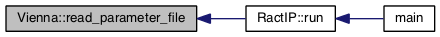
\includegraphics[width=350pt]{namespace_vienna_a3a7190f15cb9b57ffc30919582986631_icgraph}
\end{center}
\end{figure}




\subsection{Variable Documentation}
\hypertarget{namespace_vienna_a24d3b842931ab2ed27b801a9ea14b77f}{\index{Vienna@{Vienna}!eos\+\_\+debug@{eos\+\_\+debug}}
\index{eos\+\_\+debug@{eos\+\_\+debug}!Vienna@{Vienna}}
\subsubsection[{eos\+\_\+debug}]{\setlength{\rightskip}{0pt plus 5cm}int Vienna\+::eos\+\_\+debug}}\label{namespace_vienna_a24d3b842931ab2ed27b801a9ea14b77f}


Definition at line 63 of file ractip\+\_\+hom.\+cpp.

\hypertarget{namespace_vienna_a8238d1b2f4301ad0ed67a7e02c3bb4e3}{\index{Vienna@{Vienna}!pr\+\_\+duplex@{pr\+\_\+duplex}}
\index{pr\+\_\+duplex@{pr\+\_\+duplex}!Vienna@{Vienna}}
\subsubsection[{pr\+\_\+duplex}]{\setlength{\rightskip}{0pt plus 5cm}double$\ast$$\ast$ Vienna\+::pr\+\_\+duplex}}\label{namespace_vienna_a8238d1b2f4301ad0ed67a7e02c3bb4e3}


Definition at line 57 of file pf\+\_\+duplex.\+c.

\hypertarget{namespace_vienna_af212193cb67ebca5f87d42c4ab9e0196}{\index{Vienna@{Vienna}!pr\+\_\+duplex2@{pr\+\_\+duplex2}}
\index{pr\+\_\+duplex2@{pr\+\_\+duplex2}!Vienna@{Vienna}}
\subsubsection[{pr\+\_\+duplex2}]{\setlength{\rightskip}{0pt plus 5cm}double$\ast$$\ast$ Vienna\+::pr\+\_\+duplex2}}\label{namespace_vienna_af212193cb67ebca5f87d42c4ab9e0196}


Definition at line 58 of file pf\+\_\+duplex.\+c.


\chapter{Class Documentation}
\hypertarget{class_alignment}{\section{Alignment Class Reference}
\label{class_alignment}\index{Alignment@{Alignment}}
}


{\ttfamily \#include $<$alignment.\+h$>$}



Inheritance diagram for Alignment\+:
\nopagebreak
\begin{figure}[H]
\begin{center}
\leavevmode
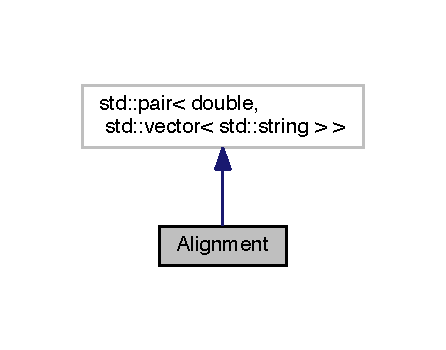
\includegraphics[width=214pt]{class_alignment__inherit__graph}
\end{center}
\end{figure}


Collaboration diagram for Alignment\+:
\nopagebreak
\begin{figure}[H]
\begin{center}
\leavevmode
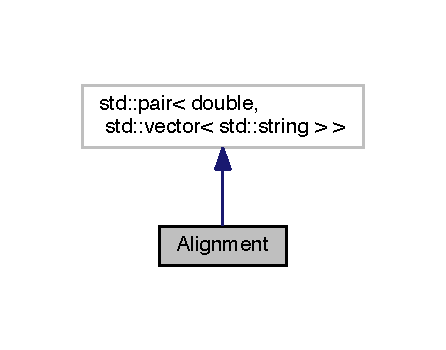
\includegraphics[width=214pt]{class_alignment__coll__graph}
\end{center}
\end{figure}
\subsection*{Public Member Functions}
\begin{DoxyCompactItemize}
\item 
\hyperlink{class_alignment_a4a77b027f01092f0b12607d92035fa15}{Alignment} (std\+::vector$<$ std\+::string $>$ seq)
\item 
double \hyperlink{class_alignment_aeb1e9bdb5ac0c4930b50709156c677a0}{get\+\_\+prob} ()
\item 
std\+::vector$<$ std\+::string $>$ \hyperlink{class_alignment_a47a90fe208b3cbdc124253126ba23a5f}{get\+\_\+seq} ()
\end{DoxyCompactItemize}


\subsection{Constructor \& Destructor Documentation}
\hypertarget{class_alignment_a4a77b027f01092f0b12607d92035fa15}{\index{Alignment@{Alignment}!Alignment@{Alignment}}
\index{Alignment@{Alignment}!Alignment@{Alignment}}
\subsubsection[{Alignment}]{\setlength{\rightskip}{0pt plus 5cm}Alignment\+::\+Alignment (
\begin{DoxyParamCaption}
\item[{std\+::vector$<$ std\+::string $>$}]{seq}
\end{DoxyParamCaption}
)\hspace{0.3cm}{\ttfamily [inline]}}}\label{class_alignment_a4a77b027f01092f0b12607d92035fa15}


\subsection{Member Function Documentation}
\hypertarget{class_alignment_aeb1e9bdb5ac0c4930b50709156c677a0}{\index{Alignment@{Alignment}!get\+\_\+prob@{get\+\_\+prob}}
\index{get\+\_\+prob@{get\+\_\+prob}!Alignment@{Alignment}}
\subsubsection[{get\+\_\+prob}]{\setlength{\rightskip}{0pt plus 5cm}double Alignment\+::get\+\_\+prob (
\begin{DoxyParamCaption}
{}
\end{DoxyParamCaption}
)\hspace{0.3cm}{\ttfamily [inline]}}}\label{class_alignment_aeb1e9bdb5ac0c4930b50709156c677a0}
\hypertarget{class_alignment_a47a90fe208b3cbdc124253126ba23a5f}{\index{Alignment@{Alignment}!get\+\_\+seq@{get\+\_\+seq}}
\index{get\+\_\+seq@{get\+\_\+seq}!Alignment@{Alignment}}
\subsubsection[{get\+\_\+seq}]{\setlength{\rightskip}{0pt plus 5cm}std\+::vector$<$std\+::string$>$ Alignment\+::get\+\_\+seq (
\begin{DoxyParamCaption}
{}
\end{DoxyParamCaption}
)\hspace{0.3cm}{\ttfamily [inline]}}}\label{class_alignment_a47a90fe208b3cbdc124253126ba23a5f}


The documentation for this class was generated from the following file\+:\begin{DoxyCompactItemize}
\item 
/\+Users/takashi/cbrc/ractip\+\_\+hom/src/\hyperlink{alignment_8h}{alignment.\+h}\end{DoxyCompactItemize}

\hypertarget{class_aln}{\section{Aln Class Reference}
\label{class_aln}\index{Aln@{Aln}}
}


{\ttfamily \#include $<$aln.\+h$>$}

\subsection*{Public Member Functions}
\begin{DoxyCompactItemize}
\item 
\hyperlink{class_aln_afb7059e932712d6d0a61857dd592c967}{Aln} ()
\item 
\hyperlink{class_aln_a97b368aa74831205e5abd35b39eaf647}{Aln} (const std\+::list$<$ std\+::string $>$ \&\hyperlink{class_aln_a1ab21509801bad54f735c9fd547c0a04}{name}, const std\+::list$<$ std\+::string $>$ \&\hyperlink{class_aln_a07ac4d997bee9b73c5d2da5fd8e0102a}{seq})
\item 
\hyperlink{class_aln_a481e0dab2dd462a6e277ad3b3982df12}{Aln} (const \hyperlink{class_aln}{Aln} \&aln)
\item 
\hyperlink{class_aln}{Aln} \& \hyperlink{class_aln_a75e300214412b357d6d382a807834d0a}{operator=} (const \hyperlink{class_aln}{Aln} \&aln)
\item 
const std\+::list$<$ std\+::string $>$ \& \hyperlink{class_aln_a1ab21509801bad54f735c9fd547c0a04}{name} () const 
\item 
const std\+::list$<$ std\+::string $>$ \& \hyperlink{class_aln_a07ac4d997bee9b73c5d2da5fd8e0102a}{seq} () const 
\item 
std\+::list$<$ std\+::string $>$ \& \hyperlink{class_aln_ab34086c2018b34082b10603eb8607a99}{seq} ()
\item 
unsigned int \hyperlink{class_aln_a2e473685aac8dc4c5bf58a2013254907}{size} () const 
\item 
unsigned int \hyperlink{class_aln_ababa37dc4967c06b20c4af1b7a42a789}{num\+\_\+aln} () const 
\item 
std\+::string \hyperlink{class_aln_a45fb6b8dcfcf254836bacabbbebe4ce8}{consensus} () const 
\item 
unsigned int \hyperlink{class_aln_a5fcc6e25e01d0cbb7fba486d0d1ee66b}{load} (B\+O\+O\+S\+T\+\_\+\+S\+P\+I\+R\+I\+T\+\_\+\+C\+L\+A\+S\+S\+I\+C\+\_\+\+N\+S\+::file\+\_\+iterator$<$$>$ \&fi)
\end{DoxyCompactItemize}
\subsection*{Static Public Member Functions}
\begin{DoxyCompactItemize}
\item 
static unsigned int \hyperlink{class_aln_a4e7552a5bf54c3a7304fd2d4ca5a14e2}{load} (std\+::list$<$ \hyperlink{class_aln}{Aln} $>$ \&data, const char $\ast$file)
\end{DoxyCompactItemize}


\subsection{Detailed Description}


Definition at line 37 of file aln.\+h.



\subsection{Constructor \& Destructor Documentation}
\hypertarget{class_aln_afb7059e932712d6d0a61857dd592c967}{\index{Aln@{Aln}!Aln@{Aln}}
\index{Aln@{Aln}!Aln@{Aln}}
\subsubsection[{Aln}]{\setlength{\rightskip}{0pt plus 5cm}Aln\+::\+Aln (
\begin{DoxyParamCaption}
{}
\end{DoxyParamCaption}
)\hspace{0.3cm}{\ttfamily [inline]}}}\label{class_aln_afb7059e932712d6d0a61857dd592c967}


Definition at line 40 of file aln.\+h.

\hypertarget{class_aln_a97b368aa74831205e5abd35b39eaf647}{\index{Aln@{Aln}!Aln@{Aln}}
\index{Aln@{Aln}!Aln@{Aln}}
\subsubsection[{Aln}]{\setlength{\rightskip}{0pt plus 5cm}Aln\+::\+Aln (
\begin{DoxyParamCaption}
\item[{const std\+::list$<$ std\+::string $>$ \&}]{name, }
\item[{const std\+::list$<$ std\+::string $>$ \&}]{seq}
\end{DoxyParamCaption}
)\hspace{0.3cm}{\ttfamily [inline]}}}\label{class_aln_a97b368aa74831205e5abd35b39eaf647}


Definition at line 43 of file aln.\+h.

\hypertarget{class_aln_a481e0dab2dd462a6e277ad3b3982df12}{\index{Aln@{Aln}!Aln@{Aln}}
\index{Aln@{Aln}!Aln@{Aln}}
\subsubsection[{Aln}]{\setlength{\rightskip}{0pt plus 5cm}Aln\+::\+Aln (
\begin{DoxyParamCaption}
\item[{const {\bf Aln} \&}]{aln}
\end{DoxyParamCaption}
)\hspace{0.3cm}{\ttfamily [inline]}}}\label{class_aln_a481e0dab2dd462a6e277ad3b3982df12}


Definition at line 48 of file aln.\+h.



\subsection{Member Function Documentation}
\hypertarget{class_aln_a45fb6b8dcfcf254836bacabbbebe4ce8}{\index{Aln@{Aln}!consensus@{consensus}}
\index{consensus@{consensus}!Aln@{Aln}}
\subsubsection[{consensus}]{\setlength{\rightskip}{0pt plus 5cm}std\+::string Aln\+::consensus (
\begin{DoxyParamCaption}
{}
\end{DoxyParamCaption}
) const}}\label{class_aln_a45fb6b8dcfcf254836bacabbbebe4ce8}


Definition at line 213 of file aln.\+cpp.



Here is the caller graph for this function\+:
\nopagebreak
\begin{figure}[H]
\begin{center}
\leavevmode
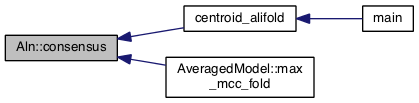
\includegraphics[width=350pt]{class_aln_a45fb6b8dcfcf254836bacabbbebe4ce8_icgraph}
\end{center}
\end{figure}


\hypertarget{class_aln_a4e7552a5bf54c3a7304fd2d4ca5a14e2}{\index{Aln@{Aln}!load@{load}}
\index{load@{load}!Aln@{Aln}}
\subsubsection[{load}]{\setlength{\rightskip}{0pt plus 5cm}unsigned int Aln\+::load (
\begin{DoxyParamCaption}
\item[{std\+::list$<$ {\bf Aln} $>$ \&}]{data, }
\item[{const char $\ast$}]{file}
\end{DoxyParamCaption}
)\hspace{0.3cm}{\ttfamily [static]}}}\label{class_aln_a4e7552a5bf54c3a7304fd2d4ca5a14e2}


Definition at line 168 of file aln.\+cpp.



Here is the call graph for this function\+:
\nopagebreak
\begin{figure}[H]
\begin{center}
\leavevmode
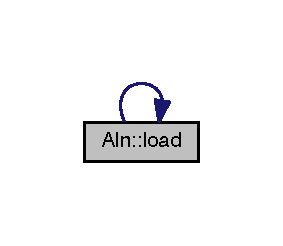
\includegraphics[width=136pt]{class_aln_a4e7552a5bf54c3a7304fd2d4ca5a14e2_cgraph}
\end{center}
\end{figure}




Here is the caller graph for this function\+:
\nopagebreak
\begin{figure}[H]
\begin{center}
\leavevmode
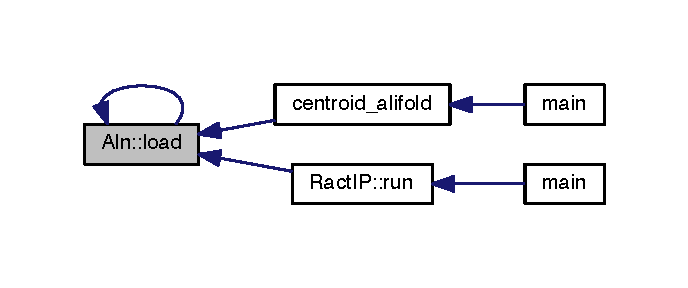
\includegraphics[width=330pt]{class_aln_a4e7552a5bf54c3a7304fd2d4ca5a14e2_icgraph}
\end{center}
\end{figure}


\hypertarget{class_aln_a5fcc6e25e01d0cbb7fba486d0d1ee66b}{\index{Aln@{Aln}!load@{load}}
\index{load@{load}!Aln@{Aln}}
\subsubsection[{load}]{\setlength{\rightskip}{0pt plus 5cm}unsigned int Aln\+::load (
\begin{DoxyParamCaption}
\item[{B\+O\+O\+S\+T\+\_\+\+S\+P\+I\+R\+I\+T\+\_\+\+C\+L\+A\+S\+S\+I\+C\+\_\+\+N\+S\+::file\+\_\+iterator$<$$>$ \&}]{fi}
\end{DoxyParamCaption}
)}}\label{class_aln_a5fcc6e25e01d0cbb7fba486d0d1ee66b}
\hypertarget{class_aln_a1ab21509801bad54f735c9fd547c0a04}{\index{Aln@{Aln}!name@{name}}
\index{name@{name}!Aln@{Aln}}
\subsubsection[{name}]{\setlength{\rightskip}{0pt plus 5cm}const std\+::list$<$std\+::string$>$\& Aln\+::name (
\begin{DoxyParamCaption}
{}
\end{DoxyParamCaption}
) const\hspace{0.3cm}{\ttfamily [inline]}}}\label{class_aln_a1ab21509801bad54f735c9fd547c0a04}


Definition at line 62 of file aln.\+h.



Here is the caller graph for this function\+:
\nopagebreak
\begin{figure}[H]
\begin{center}
\leavevmode
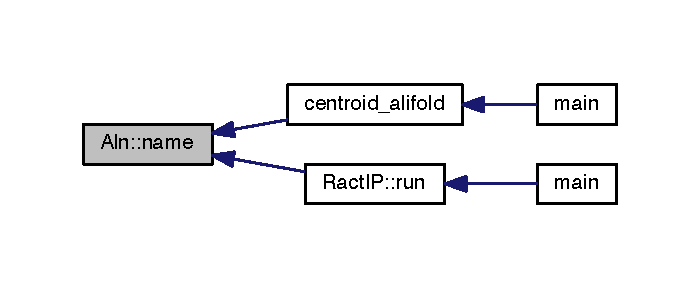
\includegraphics[width=336pt]{class_aln_a1ab21509801bad54f735c9fd547c0a04_icgraph}
\end{center}
\end{figure}


\hypertarget{class_aln_ababa37dc4967c06b20c4af1b7a42a789}{\index{Aln@{Aln}!num\+\_\+aln@{num\+\_\+aln}}
\index{num\+\_\+aln@{num\+\_\+aln}!Aln@{Aln}}
\subsubsection[{num\+\_\+aln}]{\setlength{\rightskip}{0pt plus 5cm}unsigned int Aln\+::num\+\_\+aln (
\begin{DoxyParamCaption}
{}
\end{DoxyParamCaption}
) const\hspace{0.3cm}{\ttfamily [inline]}}}\label{class_aln_ababa37dc4967c06b20c4af1b7a42a789}


Definition at line 66 of file aln.\+h.



Here is the caller graph for this function\+:
\nopagebreak
\begin{figure}[H]
\begin{center}
\leavevmode
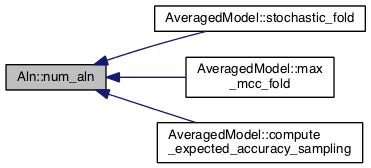
\includegraphics[width=350pt]{class_aln_ababa37dc4967c06b20c4af1b7a42a789_icgraph}
\end{center}
\end{figure}


\hypertarget{class_aln_a75e300214412b357d6d382a807834d0a}{\index{Aln@{Aln}!operator=@{operator=}}
\index{operator=@{operator=}!Aln@{Aln}}
\subsubsection[{operator=}]{\setlength{\rightskip}{0pt plus 5cm}{\bf Aln}\& Aln\+::operator= (
\begin{DoxyParamCaption}
\item[{const {\bf Aln} \&}]{aln}
\end{DoxyParamCaption}
)\hspace{0.3cm}{\ttfamily [inline]}}}\label{class_aln_a75e300214412b357d6d382a807834d0a}


Definition at line 53 of file aln.\+h.

\hypertarget{class_aln_a07ac4d997bee9b73c5d2da5fd8e0102a}{\index{Aln@{Aln}!seq@{seq}}
\index{seq@{seq}!Aln@{Aln}}
\subsubsection[{seq}]{\setlength{\rightskip}{0pt plus 5cm}const std\+::list$<$std\+::string$>$\& Aln\+::seq (
\begin{DoxyParamCaption}
{}
\end{DoxyParamCaption}
) const\hspace{0.3cm}{\ttfamily [inline]}}}\label{class_aln_a07ac4d997bee9b73c5d2da5fd8e0102a}


Definition at line 63 of file aln.\+h.



Here is the caller graph for this function\+:
\nopagebreak
\begin{figure}[H]
\begin{center}
\leavevmode
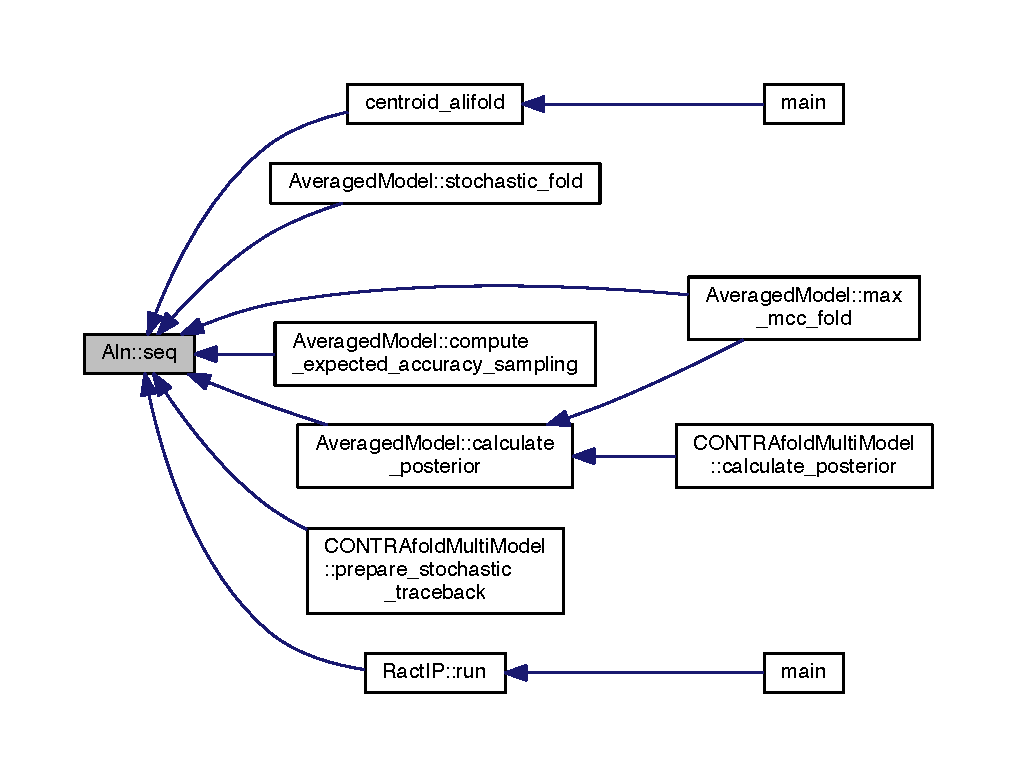
\includegraphics[width=350pt]{class_aln_a07ac4d997bee9b73c5d2da5fd8e0102a_icgraph}
\end{center}
\end{figure}


\hypertarget{class_aln_ab34086c2018b34082b10603eb8607a99}{\index{Aln@{Aln}!seq@{seq}}
\index{seq@{seq}!Aln@{Aln}}
\subsubsection[{seq}]{\setlength{\rightskip}{0pt plus 5cm}std\+::list$<$std\+::string$>$\& Aln\+::seq (
\begin{DoxyParamCaption}
{}
\end{DoxyParamCaption}
)\hspace{0.3cm}{\ttfamily [inline]}}}\label{class_aln_ab34086c2018b34082b10603eb8607a99}


Definition at line 64 of file aln.\+h.

\hypertarget{class_aln_a2e473685aac8dc4c5bf58a2013254907}{\index{Aln@{Aln}!size@{size}}
\index{size@{size}!Aln@{Aln}}
\subsubsection[{size}]{\setlength{\rightskip}{0pt plus 5cm}unsigned int Aln\+::size (
\begin{DoxyParamCaption}
{}
\end{DoxyParamCaption}
) const\hspace{0.3cm}{\ttfamily [inline]}}}\label{class_aln_a2e473685aac8dc4c5bf58a2013254907}


Definition at line 65 of file aln.\+h.



Here is the caller graph for this function\+:
\nopagebreak
\begin{figure}[H]
\begin{center}
\leavevmode
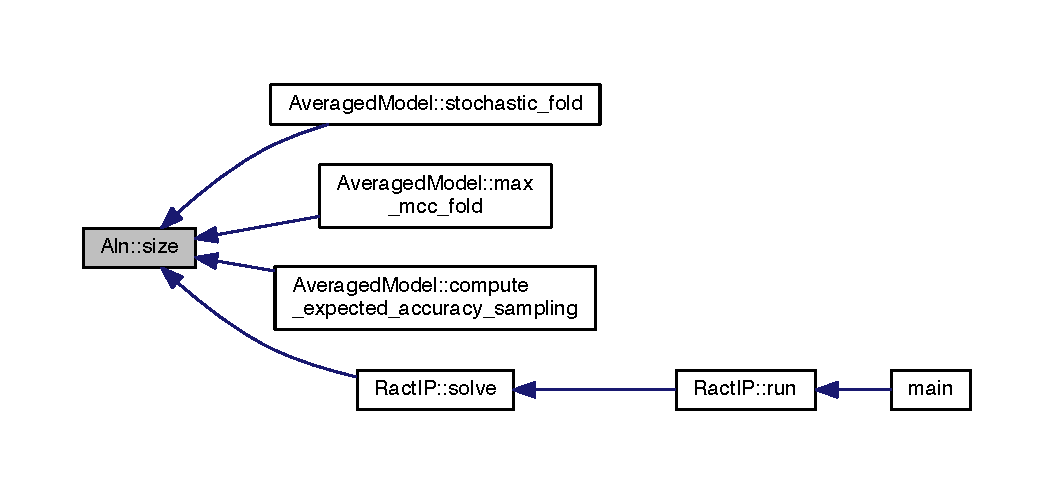
\includegraphics[width=350pt]{class_aln_a2e473685aac8dc4c5bf58a2013254907_icgraph}
\end{center}
\end{figure}




The documentation for this class was generated from the following files\+:\begin{DoxyCompactItemize}
\item 
src/centroidalifold/\hyperlink{aln_8h}{aln.\+h}\item 
src/centroidalifold/\hyperlink{aln_8cpp}{aln.\+cpp}\end{DoxyCompactItemize}

\hypertarget{structaln__parser}{\section{aln\+\_\+parser Struct Reference}
\label{structaln__parser}\index{aln\+\_\+parser@{aln\+\_\+parser}}
}


Inheritance diagram for aln\+\_\+parser\+:
\nopagebreak
\begin{figure}[H]
\begin{center}
\leavevmode
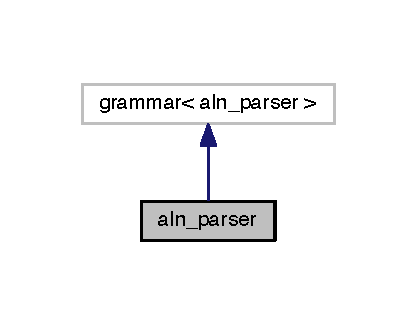
\includegraphics[width=200pt]{structaln__parser__inherit__graph}
\end{center}
\end{figure}


Collaboration diagram for aln\+\_\+parser\+:
\nopagebreak
\begin{figure}[H]
\begin{center}
\leavevmode
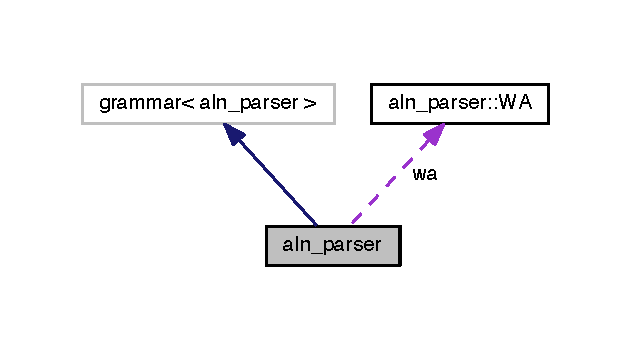
\includegraphics[width=303pt]{structaln__parser__coll__graph}
\end{center}
\end{figure}
\subsection*{Classes}
\begin{DoxyCompactItemize}
\item 
struct \hyperlink{structaln__parser_1_1definition}{definition}
\item 
class \hyperlink{classaln__parser_1_1format__error}{format\+\_\+error}
\item 
struct \hyperlink{structaln__parser_1_1push__seq}{push\+\_\+seq}
\item 
struct \hyperlink{structaln__parser_1_1reset__index}{reset\+\_\+index}
\item 
struct \hyperlink{structaln__parser_1_1_w_a}{W\+A}
\end{DoxyCompactItemize}
\subsection*{Public Member Functions}
\begin{DoxyCompactItemize}
\item 
\hyperlink{structaln__parser_a1aa7da758fdda1b61833a4ed0b0362a3}{aln\+\_\+parser} (\hyperlink{structaln__parser_1_1_w_a}{W\+A} \&x)
\end{DoxyCompactItemize}
\subsection*{Public Attributes}
\begin{DoxyCompactItemize}
\item 
\hyperlink{structaln__parser_1_1_w_a}{W\+A} \& \hyperlink{structaln__parser_a0532df33a802c0a5ed28b1baa32c9ce8}{wa}
\end{DoxyCompactItemize}


\subsection{Detailed Description}


Definition at line 51 of file aln.\+cpp.



\subsection{Constructor \& Destructor Documentation}
\hypertarget{structaln__parser_a1aa7da758fdda1b61833a4ed0b0362a3}{\index{aln\+\_\+parser@{aln\+\_\+parser}!aln\+\_\+parser@{aln\+\_\+parser}}
\index{aln\+\_\+parser@{aln\+\_\+parser}!aln\+\_\+parser@{aln\+\_\+parser}}
\subsubsection[{aln\+\_\+parser}]{\setlength{\rightskip}{0pt plus 5cm}aln\+\_\+parser\+::aln\+\_\+parser (
\begin{DoxyParamCaption}
\item[{{\bf W\+A} \&}]{x}
\end{DoxyParamCaption}
)\hspace{0.3cm}{\ttfamily [inline]}}}\label{structaln__parser_a1aa7da758fdda1b61833a4ed0b0362a3}


Definition at line 71 of file aln.\+cpp.



\subsection{Member Data Documentation}
\hypertarget{structaln__parser_a0532df33a802c0a5ed28b1baa32c9ce8}{\index{aln\+\_\+parser@{aln\+\_\+parser}!wa@{wa}}
\index{wa@{wa}!aln\+\_\+parser@{aln\+\_\+parser}}
\subsubsection[{wa}]{\setlength{\rightskip}{0pt plus 5cm}{\bf W\+A}\& aln\+\_\+parser\+::wa}}\label{structaln__parser_a0532df33a802c0a5ed28b1baa32c9ce8}


Definition at line 70 of file aln.\+cpp.



The documentation for this struct was generated from the following file\+:\begin{DoxyCompactItemize}
\item 
src/centroidalifold/\hyperlink{aln_8cpp}{aln.\+cpp}\end{DoxyCompactItemize}

\hypertarget{structfa__parser_1_1append__seq}{\section{fa\+\_\+parser\+:\+:append\+\_\+seq Struct Reference}
\label{structfa__parser_1_1append__seq}\index{fa\+\_\+parser\+::append\+\_\+seq@{fa\+\_\+parser\+::append\+\_\+seq}}
}
\subsection*{Public Member Functions}
\begin{DoxyCompactItemize}
\item 
\hyperlink{structfa__parser_1_1append__seq_ac4014e74c64af13d65fcffc3258704bd}{append\+\_\+seq} (std\+::string \&s)
\item 
{\footnotesize template$<$class Ite $>$ }\\void \hyperlink{structfa__parser_1_1append__seq_acc924c9cafca4e4380a066d897c19fa6}{operator()} (Ite i1, Ite i2) const 
\item 
\hyperlink{structfa__parser_1_1append__seq_ac4014e74c64af13d65fcffc3258704bd}{append\+\_\+seq} (std\+::string \&s)
\item 
{\footnotesize template$<$class Ite $>$ }\\void \hyperlink{structfa__parser_1_1append__seq_acc924c9cafca4e4380a066d897c19fa6}{operator()} (Ite i1, Ite i2) const 
\end{DoxyCompactItemize}
\subsection*{Public Attributes}
\begin{DoxyCompactItemize}
\item 
std\+::string \& \hyperlink{structfa__parser_1_1append__seq_a0354ac97946d852a422bdcc0a5e52a2d}{seq}
\end{DoxyCompactItemize}


\subsection{Detailed Description}


Definition at line 40 of file fa.\+cpp.



\subsection{Constructor \& Destructor Documentation}
\hypertarget{structfa__parser_1_1append__seq_ac4014e74c64af13d65fcffc3258704bd}{\index{fa\+\_\+parser\+::append\+\_\+seq@{fa\+\_\+parser\+::append\+\_\+seq}!append\+\_\+seq@{append\+\_\+seq}}
\index{append\+\_\+seq@{append\+\_\+seq}!fa\+\_\+parser\+::append\+\_\+seq@{fa\+\_\+parser\+::append\+\_\+seq}}
\subsubsection[{append\+\_\+seq}]{\setlength{\rightskip}{0pt plus 5cm}fa\+\_\+parser\+::append\+\_\+seq\+::append\+\_\+seq (
\begin{DoxyParamCaption}
\item[{std\+::string \&}]{s}
\end{DoxyParamCaption}
)\hspace{0.3cm}{\ttfamily [inline]}}}\label{structfa__parser_1_1append__seq_ac4014e74c64af13d65fcffc3258704bd}


Definition at line 44 of file fa.\+cpp.

\hypertarget{structfa__parser_1_1append__seq_ac4014e74c64af13d65fcffc3258704bd}{\index{fa\+\_\+parser\+::append\+\_\+seq@{fa\+\_\+parser\+::append\+\_\+seq}!append\+\_\+seq@{append\+\_\+seq}}
\index{append\+\_\+seq@{append\+\_\+seq}!fa\+\_\+parser\+::append\+\_\+seq@{fa\+\_\+parser\+::append\+\_\+seq}}
\subsubsection[{append\+\_\+seq}]{\setlength{\rightskip}{0pt plus 5cm}fa\+\_\+parser\+::append\+\_\+seq\+::append\+\_\+seq (
\begin{DoxyParamCaption}
\item[{std\+::string \&}]{s}
\end{DoxyParamCaption}
)\hspace{0.3cm}{\ttfamily [inline]}}}\label{structfa__parser_1_1append__seq_ac4014e74c64af13d65fcffc3258704bd}


Definition at line 44 of file fa.\+cpp.



\subsection{Member Function Documentation}
\hypertarget{structfa__parser_1_1append__seq_acc924c9cafca4e4380a066d897c19fa6}{\index{fa\+\_\+parser\+::append\+\_\+seq@{fa\+\_\+parser\+::append\+\_\+seq}!operator()@{operator()}}
\index{operator()@{operator()}!fa\+\_\+parser\+::append\+\_\+seq@{fa\+\_\+parser\+::append\+\_\+seq}}
\subsubsection[{operator()}]{\setlength{\rightskip}{0pt plus 5cm}template$<$class Ite $>$ void fa\+\_\+parser\+::append\+\_\+seq\+::operator() (
\begin{DoxyParamCaption}
\item[{Ite}]{i1, }
\item[{Ite}]{i2}
\end{DoxyParamCaption}
) const\hspace{0.3cm}{\ttfamily [inline]}}}\label{structfa__parser_1_1append__seq_acc924c9cafca4e4380a066d897c19fa6}


Definition at line 47 of file fa.\+cpp.

\hypertarget{structfa__parser_1_1append__seq_acc924c9cafca4e4380a066d897c19fa6}{\index{fa\+\_\+parser\+::append\+\_\+seq@{fa\+\_\+parser\+::append\+\_\+seq}!operator()@{operator()}}
\index{operator()@{operator()}!fa\+\_\+parser\+::append\+\_\+seq@{fa\+\_\+parser\+::append\+\_\+seq}}
\subsubsection[{operator()}]{\setlength{\rightskip}{0pt plus 5cm}template$<$class Ite $>$ void fa\+\_\+parser\+::append\+\_\+seq\+::operator() (
\begin{DoxyParamCaption}
\item[{Ite}]{i1, }
\item[{Ite}]{i2}
\end{DoxyParamCaption}
) const\hspace{0.3cm}{\ttfamily [inline]}}}\label{structfa__parser_1_1append__seq_acc924c9cafca4e4380a066d897c19fa6}


Definition at line 47 of file fa.\+cpp.



\subsection{Member Data Documentation}
\hypertarget{structfa__parser_1_1append__seq_a0354ac97946d852a422bdcc0a5e52a2d}{\index{fa\+\_\+parser\+::append\+\_\+seq@{fa\+\_\+parser\+::append\+\_\+seq}!seq@{seq}}
\index{seq@{seq}!fa\+\_\+parser\+::append\+\_\+seq@{fa\+\_\+parser\+::append\+\_\+seq}}
\subsubsection[{seq}]{\setlength{\rightskip}{0pt plus 5cm}std\+::string \& fa\+\_\+parser\+::append\+\_\+seq\+::seq}}\label{structfa__parser_1_1append__seq_a0354ac97946d852a422bdcc0a5e52a2d}


Definition at line 42 of file fa.\+cpp.



The documentation for this struct was generated from the following file\+:\begin{DoxyCompactItemize}
\item 
src/centroidalifold/\hyperlink{centroidalifold_2fa_8cpp}{fa.\+cpp}\end{DoxyCompactItemize}

\hypertarget{class_aux_model}{\section{Aux\+Model Class Reference}
\label{class_aux_model}\index{Aux\+Model@{Aux\+Model}}
}


{\ttfamily \#include $<$aux.\+h$>$}



Inheritance diagram for Aux\+Model\+:
\nopagebreak
\begin{figure}[H]
\begin{center}
\leavevmode
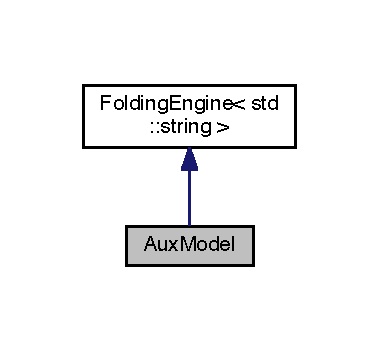
\includegraphics[width=182pt]{class_aux_model__inherit__graph}
\end{center}
\end{figure}


Collaboration diagram for Aux\+Model\+:
\nopagebreak
\begin{figure}[H]
\begin{center}
\leavevmode
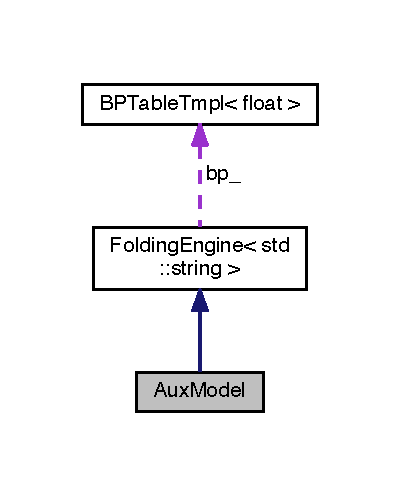
\includegraphics[width=192pt]{class_aux_model__coll__graph}
\end{center}
\end{figure}
\subsection*{Public Member Functions}
\begin{DoxyCompactItemize}
\item 
\hyperlink{class_aux_model_a3593c40ae6fb3c7143365fdf9784b6bf}{Aux\+Model} (const std\+::vector$<$ std\+::string $>$ \&bpfiles, bool run\+\_\+as\+\_\+mea=\hyperlink{naview_8c_a65e9886d74aaee76545e83dd09011727}{false})
\item 
virtual \hyperlink{class_aux_model_ae796ee47f2d0255c48be4b62a3811e70}{$\sim$\+Aux\+Model} ()
\item 
virtual void \hyperlink{class_aux_model_aa0351133a58e0038f55580dbf4f925c8}{calculate\+\_\+posterior} (const std\+::string \&seq)
\end{DoxyCompactItemize}
\subsection*{Additional Inherited Members}


\subsection{Detailed Description}


Definition at line 29 of file aux.\+h.



\subsection{Constructor \& Destructor Documentation}
\hypertarget{class_aux_model_a3593c40ae6fb3c7143365fdf9784b6bf}{\index{Aux\+Model@{Aux\+Model}!Aux\+Model@{Aux\+Model}}
\index{Aux\+Model@{Aux\+Model}!Aux\+Model@{Aux\+Model}}
\subsubsection[{Aux\+Model}]{\setlength{\rightskip}{0pt plus 5cm}Aux\+Model\+::\+Aux\+Model (
\begin{DoxyParamCaption}
\item[{const std\+::vector$<$ std\+::string $>$ \&}]{bpfiles, }
\item[{bool}]{run\+\_\+as\+\_\+mea = {\ttfamily {\bf false}}}
\end{DoxyParamCaption}
)}}\label{class_aux_model_a3593c40ae6fb3c7143365fdf9784b6bf}


Definition at line 30 of file aux.\+cpp.

\hypertarget{class_aux_model_ae796ee47f2d0255c48be4b62a3811e70}{\index{Aux\+Model@{Aux\+Model}!````~Aux\+Model@{$\sim$\+Aux\+Model}}
\index{````~Aux\+Model@{$\sim$\+Aux\+Model}!Aux\+Model@{Aux\+Model}}
\subsubsection[{$\sim$\+Aux\+Model}]{\setlength{\rightskip}{0pt plus 5cm}virtual Aux\+Model\+::$\sim$\+Aux\+Model (
\begin{DoxyParamCaption}
{}
\end{DoxyParamCaption}
)\hspace{0.3cm}{\ttfamily [inline]}, {\ttfamily [virtual]}}}\label{class_aux_model_ae796ee47f2d0255c48be4b62a3811e70}


Definition at line 33 of file aux.\+h.



\subsection{Member Function Documentation}
\hypertarget{class_aux_model_aa0351133a58e0038f55580dbf4f925c8}{\index{Aux\+Model@{Aux\+Model}!calculate\+\_\+posterior@{calculate\+\_\+posterior}}
\index{calculate\+\_\+posterior@{calculate\+\_\+posterior}!Aux\+Model@{Aux\+Model}}
\subsubsection[{calculate\+\_\+posterior}]{\setlength{\rightskip}{0pt plus 5cm}void Aux\+Model\+::calculate\+\_\+posterior (
\begin{DoxyParamCaption}
\item[{const std\+::string \&}]{seq}
\end{DoxyParamCaption}
)\hspace{0.3cm}{\ttfamily [virtual]}}}\label{class_aux_model_aa0351133a58e0038f55580dbf4f925c8}


Implements \hyperlink{class_folding_engine_a314c78e5fe35d5a1b5f441604c58e8f1}{Folding\+Engine$<$ std\+::string $>$}.



Definition at line 37 of file aux.\+cpp.



Here is the call graph for this function\+:
\nopagebreak
\begin{figure}[H]
\begin{center}
\leavevmode
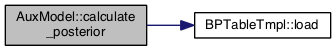
\includegraphics[width=324pt]{class_aux_model_aa0351133a58e0038f55580dbf4f925c8_cgraph}
\end{center}
\end{figure}




The documentation for this class was generated from the following files\+:\begin{DoxyCompactItemize}
\item 
src/centroidalifold/engine/\hyperlink{aux_8h}{aux.\+h}\item 
src/centroidalifold/engine/\hyperlink{aux_8cpp}{aux.\+cpp}\end{DoxyCompactItemize}

\hypertarget{struct_average_b_p}{\section{Average\+B\+P Struct Reference}
\label{struct_average_b_p}\index{Average\+B\+P@{Average\+B\+P}}
}
\subsection*{Public Member Functions}
\begin{DoxyCompactItemize}
\item 
\hyperlink{struct_average_b_p_adeba5e0514aa7ce17aaaa1e159e2872e}{Average\+B\+P} (\hyperlink{folding__engine_8h_a065821fb17bbd8df315f2435c973e3c1}{B\+P\+Table} \&bp, const std\+::list$<$ \hyperlink{folding__engine_8h_a719ce23ace10f4f5203cee19f70e11eb}{B\+P\+Table\+Ptr} $>$ \&bps, const std\+::list$<$ std\+::vector$<$ \hyperlink{cyktable_8h_a91ad9478d81a7aaf2593e8d9c3d06a14}{uint} $>$ $>$ \&idxmap, \hyperlink{cyktable_8h_a91ad9478d81a7aaf2593e8d9c3d06a14}{uint} max\+\_\+dist)
\item 
void \hyperlink{struct_average_b_p_a1b54bbf8a9300ab110f829bc111e9e4c}{operator()} (\hyperlink{cyktable_8h_a91ad9478d81a7aaf2593e8d9c3d06a14}{uint} i, \hyperlink{cyktable_8h_a91ad9478d81a7aaf2593e8d9c3d06a14}{uint} j)
\item 
void \hyperlink{struct_average_b_p_aafec28a98d39cda263b9912eae89d4fc}{make} ()
\end{DoxyCompactItemize}


\subsection{Detailed Description}


Definition at line 69 of file averaged.\+cpp.



\subsection{Constructor \& Destructor Documentation}
\hypertarget{struct_average_b_p_adeba5e0514aa7ce17aaaa1e159e2872e}{\index{Average\+B\+P@{Average\+B\+P}!Average\+B\+P@{Average\+B\+P}}
\index{Average\+B\+P@{Average\+B\+P}!Average\+B\+P@{Average\+B\+P}}
\subsubsection[{Average\+B\+P}]{\setlength{\rightskip}{0pt plus 5cm}Average\+B\+P\+::\+Average\+B\+P (
\begin{DoxyParamCaption}
\item[{{\bf B\+P\+Table} \&}]{bp, }
\item[{const std\+::list$<$ {\bf B\+P\+Table\+Ptr} $>$ \&}]{bps, }
\item[{const std\+::list$<$ std\+::vector$<$ {\bf uint} $>$ $>$ \&}]{idxmap, }
\item[{{\bf uint}}]{max\+\_\+dist}
\end{DoxyParamCaption}
)\hspace{0.3cm}{\ttfamily [inline]}}}\label{struct_average_b_p_adeba5e0514aa7ce17aaaa1e159e2872e}


Definition at line 71 of file averaged.\+cpp.



\subsection{Member Function Documentation}
\hypertarget{struct_average_b_p_aafec28a98d39cda263b9912eae89d4fc}{\index{Average\+B\+P@{Average\+B\+P}!make@{make}}
\index{make@{make}!Average\+B\+P@{Average\+B\+P}}
\subsubsection[{make}]{\setlength{\rightskip}{0pt plus 5cm}void Average\+B\+P\+::make (
\begin{DoxyParamCaption}
{}
\end{DoxyParamCaption}
)\hspace{0.3cm}{\ttfamily [inline]}}}\label{struct_average_b_p_aafec28a98d39cda263b9912eae89d4fc}


Definition at line 94 of file averaged.\+cpp.



Here is the call graph for this function\+:
\nopagebreak
\begin{figure}[H]
\begin{center}
\leavevmode
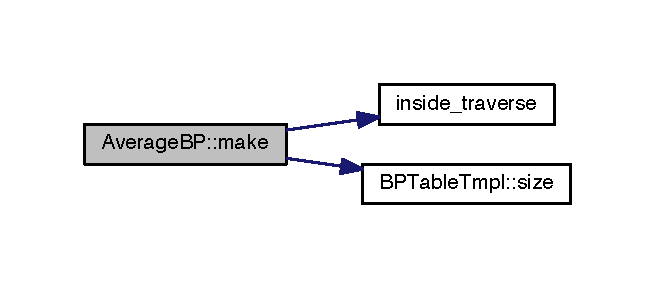
\includegraphics[width=314pt]{struct_average_b_p_aafec28a98d39cda263b9912eae89d4fc_cgraph}
\end{center}
\end{figure}




Here is the caller graph for this function\+:
\nopagebreak
\begin{figure}[H]
\begin{center}
\leavevmode
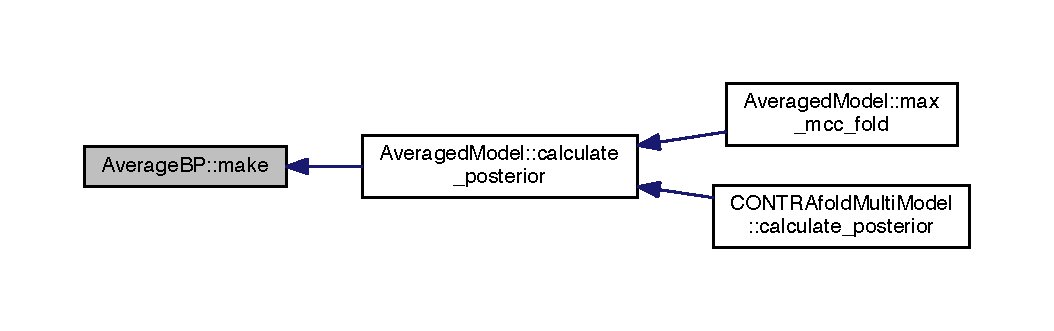
\includegraphics[width=350pt]{struct_average_b_p_aafec28a98d39cda263b9912eae89d4fc_icgraph}
\end{center}
\end{figure}


\hypertarget{struct_average_b_p_a1b54bbf8a9300ab110f829bc111e9e4c}{\index{Average\+B\+P@{Average\+B\+P}!operator()@{operator()}}
\index{operator()@{operator()}!Average\+B\+P@{Average\+B\+P}}
\subsubsection[{operator()}]{\setlength{\rightskip}{0pt plus 5cm}void Average\+B\+P\+::operator() (
\begin{DoxyParamCaption}
\item[{{\bf uint}}]{i, }
\item[{{\bf uint}}]{j}
\end{DoxyParamCaption}
)\hspace{0.3cm}{\ttfamily [inline]}}}\label{struct_average_b_p_a1b54bbf8a9300ab110f829bc111e9e4c}


Definition at line 79 of file averaged.\+cpp.



Here is the call graph for this function\+:
\nopagebreak
\begin{figure}[H]
\begin{center}
\leavevmode
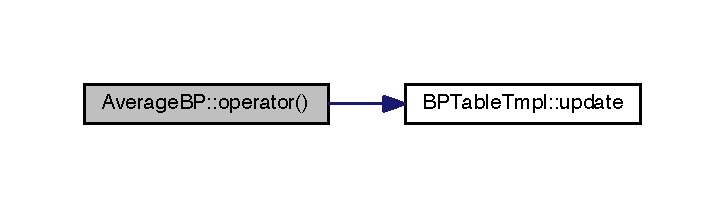
\includegraphics[width=348pt]{struct_average_b_p_a1b54bbf8a9300ab110f829bc111e9e4c_cgraph}
\end{center}
\end{figure}




The documentation for this struct was generated from the following file\+:\begin{DoxyCompactItemize}
\item 
src/centroidalifold/engine/\hyperlink{averaged_8cpp}{averaged.\+cpp}\end{DoxyCompactItemize}

\hypertarget{class_averaged_model}{\section{Averaged\+Model Class Reference}
\label{class_averaged_model}\index{Averaged\+Model@{Averaged\+Model}}
}


{\ttfamily \#include $<$averaged.\+h$>$}



Inheritance diagram for Averaged\+Model\+:
\nopagebreak
\begin{figure}[H]
\begin{center}
\leavevmode
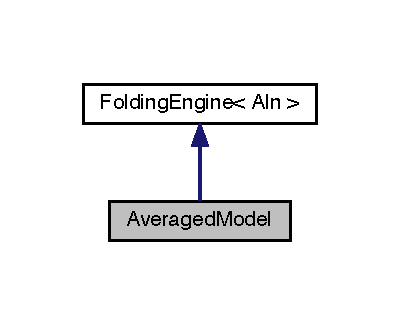
\includegraphics[width=192pt]{class_averaged_model__inherit__graph}
\end{center}
\end{figure}


Collaboration diagram for Averaged\+Model\+:
\nopagebreak
\begin{figure}[H]
\begin{center}
\leavevmode
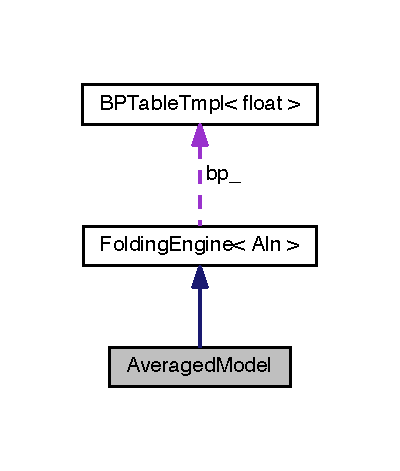
\includegraphics[width=192pt]{class_averaged_model__coll__graph}
\end{center}
\end{figure}
\subsection*{Public Member Functions}
\begin{DoxyCompactItemize}
\item 
\hyperlink{class_averaged_model_a3d502ea18660e17aba329747eafd84a9}{Averaged\+Model} (\hyperlink{class_folding_engine}{Folding\+Engine}$<$ std\+::string $>$ $\ast$\hyperlink{notespace_8cpp_ace32c53d52804f2843ccfe220db6038c}{cf}, \hyperlink{cyktable_8h_a91ad9478d81a7aaf2593e8d9c3d06a14}{uint} max\+\_\+bp\+\_\+dist, bool run\+\_\+as\+\_\+mea=\hyperlink{naview_8c_a65e9886d74aaee76545e83dd09011727}{false})
\item 
virtual \hyperlink{class_averaged_model_a2539e2282f0f4bb70145f9fb19bc2567}{$\sim$\+Averaged\+Model} ()
\item 
virtual void \hyperlink{class_averaged_model_a8b07acaf0d63c249cdc78dc1b2df7307}{stochastic\+\_\+fold} (const \hyperlink{class_aln}{Aln} \&aln, \hyperlink{cyktable_8h_a91ad9478d81a7aaf2593e8d9c3d06a14}{uint} num\+\_\+samples, std\+::ostream \&out)
\item 
virtual void \hyperlink{class_averaged_model_a65ce78340130f4ddb19b0b5782244a1b}{stochastic\+\_\+fold} (const \hyperlink{class_aln}{Aln} \&aln, \hyperlink{cyktable_8h_a91ad9478d81a7aaf2593e8d9c3d06a14}{uint} num\+\_\+samples, std\+::vector$<$ \hyperlink{folding__engine_8h_ad0a64ba9a92681778af5917fd1bbd40c}{B\+Pvec\+Ptr} $>$ \&bpv)
\item 
virtual void \hyperlink{class_averaged_model_a4844fe73e623329659ab409d8acede57}{max\+\_\+mcc\+\_\+fold} (const std\+::string \&name, const \hyperlink{class_aln}{Aln} \&aln, std\+::ostream \&out, \hyperlink{cyktable_8h_a91ad9478d81a7aaf2593e8d9c3d06a14}{uint} num\+\_\+samples)
\item 
virtual void \hyperlink{class_averaged_model_a45c8b5f77c83da55a8f19660b9319e03}{compute\+\_\+expected\+\_\+accuracy\+\_\+sampling} (const std\+::string \&paren, const \hyperlink{class_aln}{Aln} \&aln, \hyperlink{cyktable_8h_a91ad9478d81a7aaf2593e8d9c3d06a14}{uint} num\+\_\+ea\+\_\+samples, double \&sen, double \&ppv, double \&mcc)
\item 
virtual void \hyperlink{class_averaged_model_a0a261a8fe29b8b7bd00acf7eaeecf396}{set\+\_\+constraint} (const std\+::string \&str)
\item 
virtual void \hyperlink{class_averaged_model_ab594bb3e99a3e07efcdda8cf5ca001ab}{calculate\+\_\+posterior} (const \hyperlink{class_aln}{Aln} \&aln)
\end{DoxyCompactItemize}
\subsection*{Additional Inherited Members}


\subsection{Detailed Description}


Definition at line 29 of file averaged.\+h.



\subsection{Constructor \& Destructor Documentation}
\hypertarget{class_averaged_model_a3d502ea18660e17aba329747eafd84a9}{\index{Averaged\+Model@{Averaged\+Model}!Averaged\+Model@{Averaged\+Model}}
\index{Averaged\+Model@{Averaged\+Model}!Averaged\+Model@{Averaged\+Model}}
\subsubsection[{Averaged\+Model}]{\setlength{\rightskip}{0pt plus 5cm}Averaged\+Model\+::\+Averaged\+Model (
\begin{DoxyParamCaption}
\item[{{\bf Folding\+Engine}$<$ std\+::string $>$ $\ast$}]{cf, }
\item[{{\bf uint}}]{max\+\_\+bp\+\_\+dist, }
\item[{bool}]{run\+\_\+as\+\_\+mea = {\ttfamily {\bf false}}}
\end{DoxyParamCaption}
)}}\label{class_averaged_model_a3d502ea18660e17aba329747eafd84a9}


Definition at line 110 of file averaged.\+cpp.

\hypertarget{class_averaged_model_a2539e2282f0f4bb70145f9fb19bc2567}{\index{Averaged\+Model@{Averaged\+Model}!````~Averaged\+Model@{$\sim$\+Averaged\+Model}}
\index{````~Averaged\+Model@{$\sim$\+Averaged\+Model}!Averaged\+Model@{Averaged\+Model}}
\subsubsection[{$\sim$\+Averaged\+Model}]{\setlength{\rightskip}{0pt plus 5cm}virtual Averaged\+Model\+::$\sim$\+Averaged\+Model (
\begin{DoxyParamCaption}
{}
\end{DoxyParamCaption}
)\hspace{0.3cm}{\ttfamily [inline]}, {\ttfamily [virtual]}}}\label{class_averaged_model_a2539e2282f0f4bb70145f9fb19bc2567}


Definition at line 33 of file averaged.\+h.



\subsection{Member Function Documentation}
\hypertarget{class_averaged_model_ab594bb3e99a3e07efcdda8cf5ca001ab}{\index{Averaged\+Model@{Averaged\+Model}!calculate\+\_\+posterior@{calculate\+\_\+posterior}}
\index{calculate\+\_\+posterior@{calculate\+\_\+posterior}!Averaged\+Model@{Averaged\+Model}}
\subsubsection[{calculate\+\_\+posterior}]{\setlength{\rightskip}{0pt plus 5cm}void Averaged\+Model\+::calculate\+\_\+posterior (
\begin{DoxyParamCaption}
\item[{const {\bf Aln} \&}]{aln}
\end{DoxyParamCaption}
)\hspace{0.3cm}{\ttfamily [virtual]}}}\label{class_averaged_model_ab594bb3e99a3e07efcdda8cf5ca001ab}


Implements \hyperlink{class_folding_engine_a314c78e5fe35d5a1b5f441604c58e8f1}{Folding\+Engine$<$ Aln $>$}.



Definition at line 317 of file averaged.\+cpp.



Here is the call graph for this function\+:
\nopagebreak
\begin{figure}[H]
\begin{center}
\leavevmode
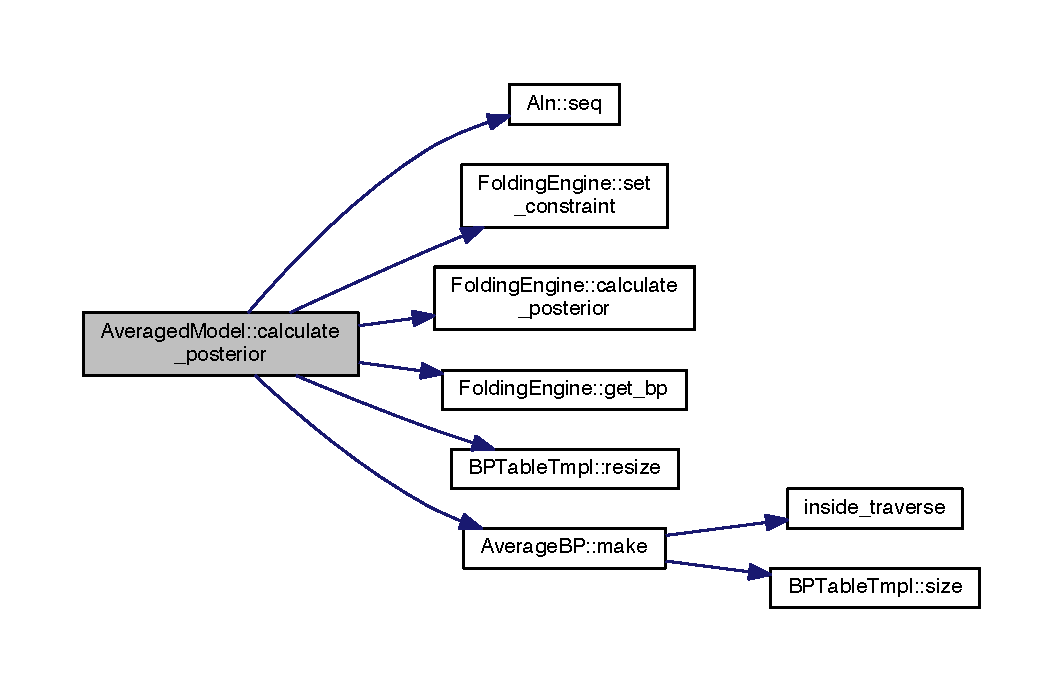
\includegraphics[width=350pt]{class_averaged_model_ab594bb3e99a3e07efcdda8cf5ca001ab_cgraph}
\end{center}
\end{figure}




Here is the caller graph for this function\+:
\nopagebreak
\begin{figure}[H]
\begin{center}
\leavevmode
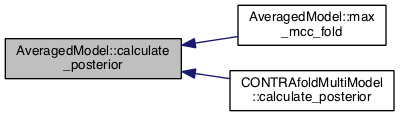
\includegraphics[width=350pt]{class_averaged_model_ab594bb3e99a3e07efcdda8cf5ca001ab_icgraph}
\end{center}
\end{figure}


\hypertarget{class_averaged_model_a45c8b5f77c83da55a8f19660b9319e03}{\index{Averaged\+Model@{Averaged\+Model}!compute\+\_\+expected\+\_\+accuracy\+\_\+sampling@{compute\+\_\+expected\+\_\+accuracy\+\_\+sampling}}
\index{compute\+\_\+expected\+\_\+accuracy\+\_\+sampling@{compute\+\_\+expected\+\_\+accuracy\+\_\+sampling}!Averaged\+Model@{Averaged\+Model}}
\subsubsection[{compute\+\_\+expected\+\_\+accuracy\+\_\+sampling}]{\setlength{\rightskip}{0pt plus 5cm}void Averaged\+Model\+::compute\+\_\+expected\+\_\+accuracy\+\_\+sampling (
\begin{DoxyParamCaption}
\item[{const std\+::string \&}]{paren, }
\item[{const {\bf Aln} \&}]{aln, }
\item[{{\bf uint}}]{num\+\_\+ea\+\_\+samples, }
\item[{double \&}]{sen, }
\item[{double \&}]{ppv, }
\item[{double \&}]{mcc}
\end{DoxyParamCaption}
)\hspace{0.3cm}{\ttfamily [virtual]}}}\label{class_averaged_model_a45c8b5f77c83da55a8f19660b9319e03}


Reimplemented from \hyperlink{class_folding_engine_ae6cbbe3009c8ff7dae235ca98ccb18c2}{Folding\+Engine$<$ Aln $>$}.



Definition at line 236 of file averaged.\+cpp.



Here is the call graph for this function\+:
\nopagebreak
\begin{figure}[H]
\begin{center}
\leavevmode
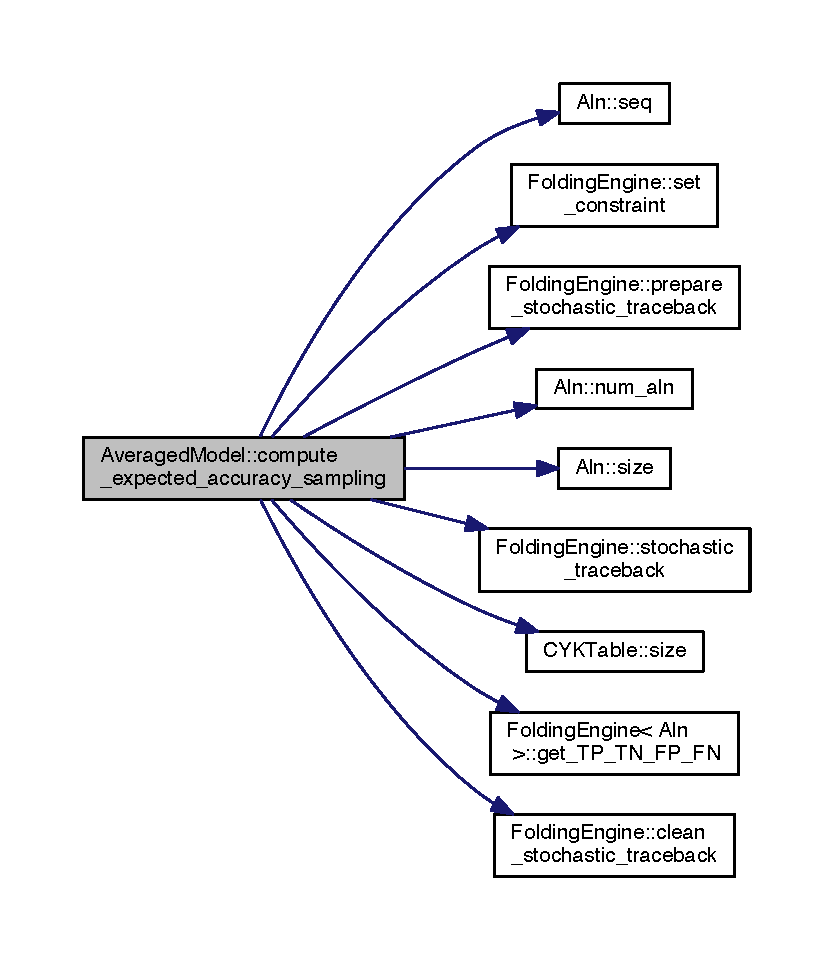
\includegraphics[width=350pt]{class_averaged_model_a45c8b5f77c83da55a8f19660b9319e03_cgraph}
\end{center}
\end{figure}


\hypertarget{class_averaged_model_a4844fe73e623329659ab409d8acede57}{\index{Averaged\+Model@{Averaged\+Model}!max\+\_\+mcc\+\_\+fold@{max\+\_\+mcc\+\_\+fold}}
\index{max\+\_\+mcc\+\_\+fold@{max\+\_\+mcc\+\_\+fold}!Averaged\+Model@{Averaged\+Model}}
\subsubsection[{max\+\_\+mcc\+\_\+fold}]{\setlength{\rightskip}{0pt plus 5cm}void Averaged\+Model\+::max\+\_\+mcc\+\_\+fold (
\begin{DoxyParamCaption}
\item[{const std\+::string \&}]{name, }
\item[{const {\bf Aln} \&}]{aln, }
\item[{std\+::ostream \&}]{out, }
\item[{{\bf uint}}]{num\+\_\+samples}
\end{DoxyParamCaption}
)\hspace{0.3cm}{\ttfamily [virtual]}}}\label{class_averaged_model_a4844fe73e623329659ab409d8acede57}


Reimplemented from \hyperlink{class_folding_engine_a387a1625b31056030998eddcada4c036}{Folding\+Engine$<$ Aln $>$}.



Definition at line 187 of file averaged.\+cpp.



Here is the call graph for this function\+:
\nopagebreak
\begin{figure}[H]
\begin{center}
\leavevmode
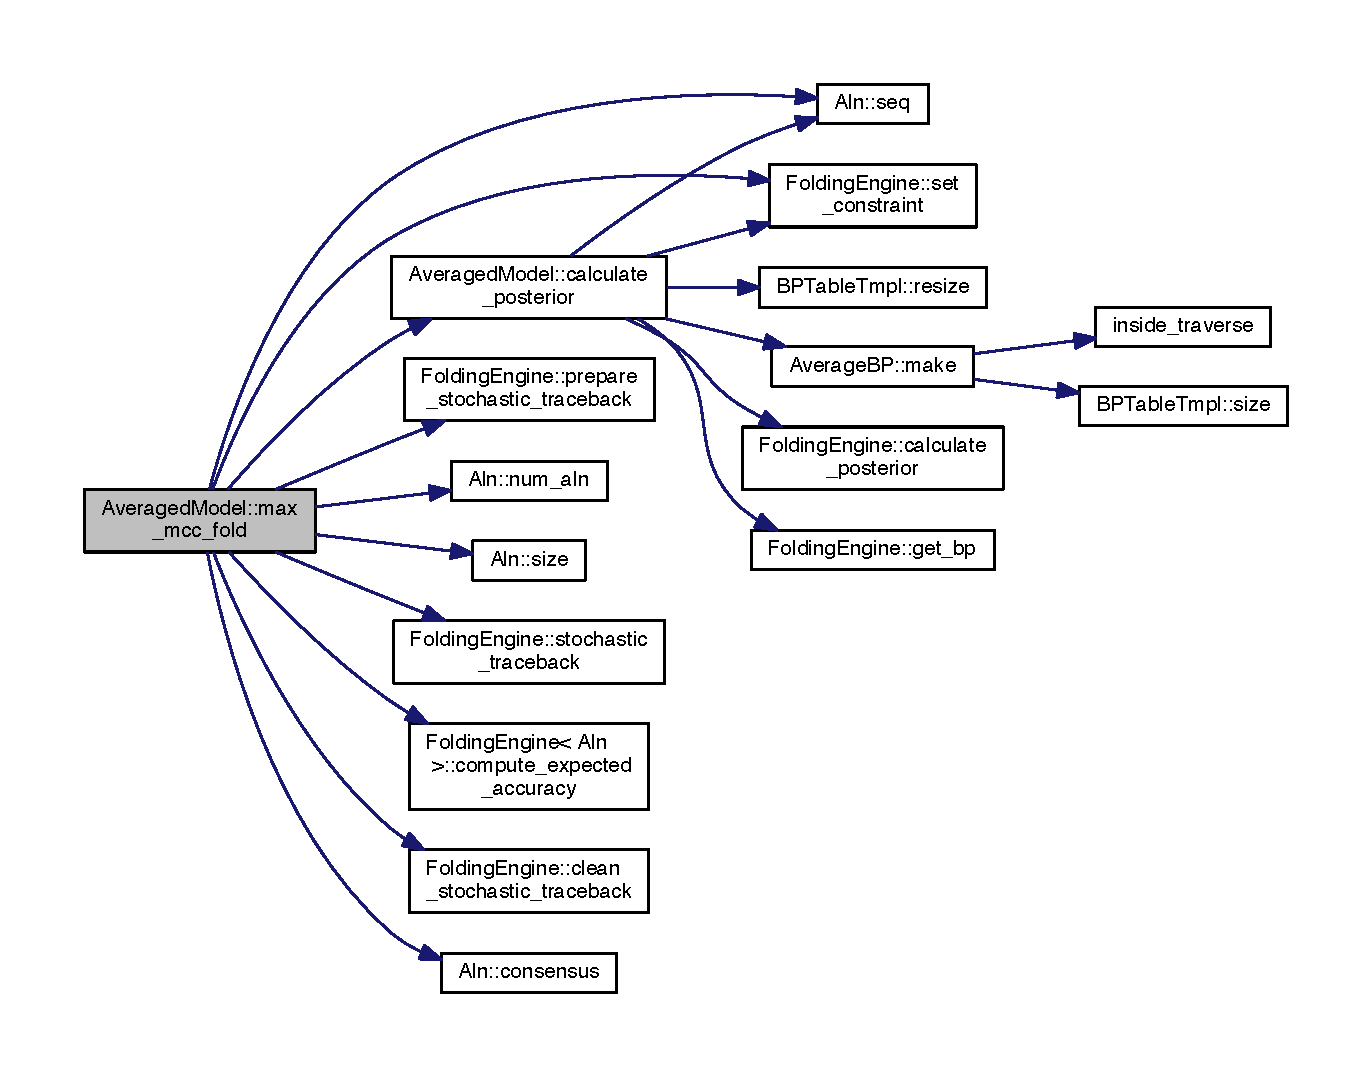
\includegraphics[width=350pt]{class_averaged_model_a4844fe73e623329659ab409d8acede57_cgraph}
\end{center}
\end{figure}


\hypertarget{class_averaged_model_a0a261a8fe29b8b7bd00acf7eaeecf396}{\index{Averaged\+Model@{Averaged\+Model}!set\+\_\+constraint@{set\+\_\+constraint}}
\index{set\+\_\+constraint@{set\+\_\+constraint}!Averaged\+Model@{Averaged\+Model}}
\subsubsection[{set\+\_\+constraint}]{\setlength{\rightskip}{0pt plus 5cm}void Averaged\+Model\+::set\+\_\+constraint (
\begin{DoxyParamCaption}
\item[{const std\+::string \&}]{str}
\end{DoxyParamCaption}
)\hspace{0.3cm}{\ttfamily [virtual]}}}\label{class_averaged_model_a0a261a8fe29b8b7bd00acf7eaeecf396}


Reimplemented from \hyperlink{class_folding_engine_aa979adbd342b75eb947927e6ff7bcb8c}{Folding\+Engine$<$ Aln $>$}.



Definition at line 294 of file averaged.\+cpp.

\hypertarget{class_averaged_model_a8b07acaf0d63c249cdc78dc1b2df7307}{\index{Averaged\+Model@{Averaged\+Model}!stochastic\+\_\+fold@{stochastic\+\_\+fold}}
\index{stochastic\+\_\+fold@{stochastic\+\_\+fold}!Averaged\+Model@{Averaged\+Model}}
\subsubsection[{stochastic\+\_\+fold}]{\setlength{\rightskip}{0pt plus 5cm}void Averaged\+Model\+::stochastic\+\_\+fold (
\begin{DoxyParamCaption}
\item[{const {\bf Aln} \&}]{aln, }
\item[{{\bf uint}}]{num\+\_\+samples, }
\item[{std\+::ostream \&}]{out}
\end{DoxyParamCaption}
)\hspace{0.3cm}{\ttfamily [virtual]}}}\label{class_averaged_model_a8b07acaf0d63c249cdc78dc1b2df7307}


Reimplemented from \hyperlink{class_folding_engine_af42fb74e518d56eaddaab33696b0d32f}{Folding\+Engine$<$ Aln $>$}.



Definition at line 117 of file averaged.\+cpp.



Here is the call graph for this function\+:
\nopagebreak
\begin{figure}[H]
\begin{center}
\leavevmode
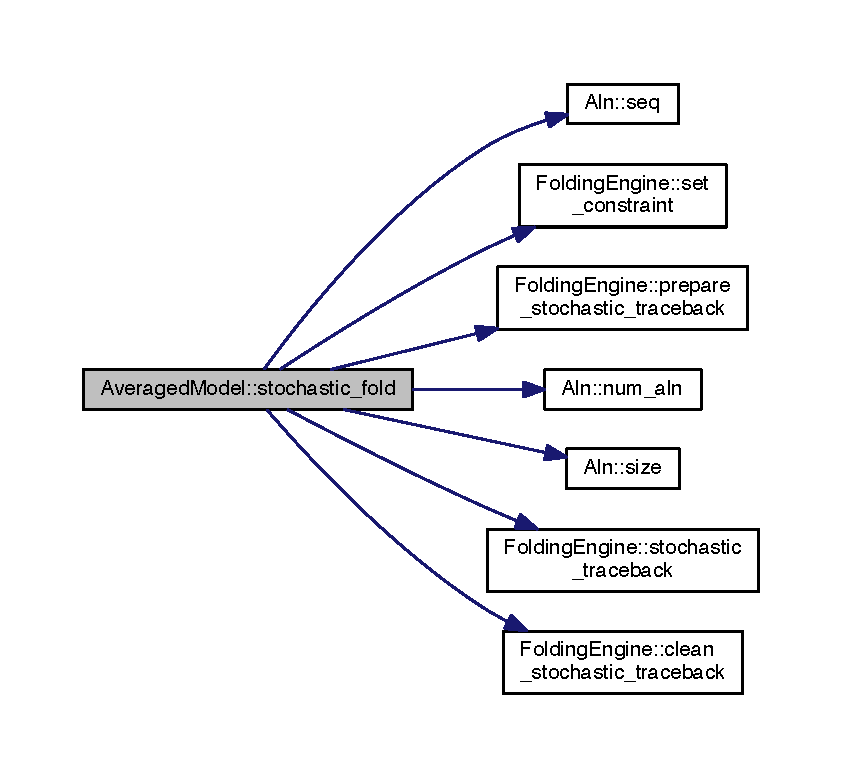
\includegraphics[width=350pt]{class_averaged_model_a8b07acaf0d63c249cdc78dc1b2df7307_cgraph}
\end{center}
\end{figure}


\hypertarget{class_averaged_model_a65ce78340130f4ddb19b0b5782244a1b}{\index{Averaged\+Model@{Averaged\+Model}!stochastic\+\_\+fold@{stochastic\+\_\+fold}}
\index{stochastic\+\_\+fold@{stochastic\+\_\+fold}!Averaged\+Model@{Averaged\+Model}}
\subsubsection[{stochastic\+\_\+fold}]{\setlength{\rightskip}{0pt plus 5cm}void Averaged\+Model\+::stochastic\+\_\+fold (
\begin{DoxyParamCaption}
\item[{const {\bf Aln} \&}]{aln, }
\item[{{\bf uint}}]{num\+\_\+samples, }
\item[{std\+::vector$<$ {\bf B\+Pvec\+Ptr} $>$ \&}]{bpv}
\end{DoxyParamCaption}
)\hspace{0.3cm}{\ttfamily [virtual]}}}\label{class_averaged_model_a65ce78340130f4ddb19b0b5782244a1b}


Reimplemented from \hyperlink{class_folding_engine_a3a83796b8f2eba402e90fb726c167680}{Folding\+Engine$<$ Aln $>$}.



Definition at line 153 of file averaged.\+cpp.



Here is the call graph for this function\+:
\nopagebreak
\begin{figure}[H]
\begin{center}
\leavevmode
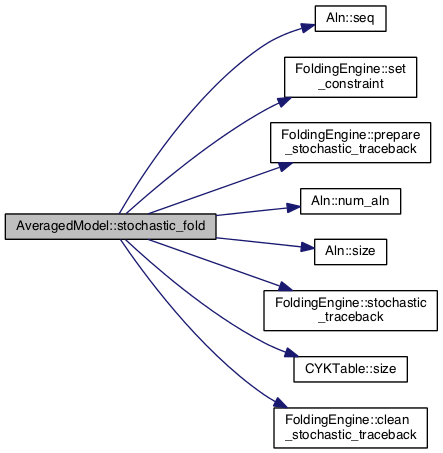
\includegraphics[width=350pt]{class_averaged_model_a65ce78340130f4ddb19b0b5782244a1b_cgraph}
\end{center}
\end{figure}




The documentation for this class was generated from the following files\+:\begin{DoxyCompactItemize}
\item 
src/centroidalifold/engine/\hyperlink{averaged_8h}{averaged.\+h}\item 
src/centroidalifold/engine/\hyperlink{averaged_8cpp}{averaged.\+cpp}\end{DoxyCompactItemize}

\hypertarget{class_b_p_table_tmpl}{\section{B\+P\+Table\+Tmpl$<$ T $>$ Class Template Reference}
\label{class_b_p_table_tmpl}\index{B\+P\+Table\+Tmpl$<$ T $>$@{B\+P\+Table\+Tmpl$<$ T $>$}}
}


{\ttfamily \#include $<$bp.\+h$>$}

\subsection*{Public Types}
\begin{DoxyCompactItemize}
\item 
typedef T \hyperlink{class_b_p_table_tmpl_abeaa8313585c7a571fae9d26211432a6}{value\+\_\+type}
\end{DoxyCompactItemize}
\subsection*{Public Member Functions}
\begin{DoxyCompactItemize}
\item 
\hyperlink{class_b_p_table_tmpl_a78a5662bc3049d62f7758f2752530fae}{B\+P\+Table\+Tmpl} ()
\item 
\hyperlink{class_b_p_table_tmpl_aec4290a9480e2a3204ac03f8fb7214f9}{B\+P\+Table\+Tmpl} (\hyperlink{cyktable_8h_a91ad9478d81a7aaf2593e8d9c3d06a14}{uint} sz, \hyperlink{cyktable_8h_a91ad9478d81a7aaf2593e8d9c3d06a14}{uint} \hyperlink{class_b_p_table_tmpl_a5e74154a1f5ba441b95f910fbb4a6e89}{max\+\_\+dist}=0)
\item 
\hyperlink{class_b_p_table_tmpl_aae0a91abdb1a0c81a6d9fd88d5db3c0d}{B\+P\+Table\+Tmpl} (const \hyperlink{class_b_p_table_tmpl}{B\+P\+Table\+Tmpl} \&x)
\item 
void \hyperlink{class_b_p_table_tmpl_aab197cc5c6d5088f5789c08f1280a3a5}{reserve} (\hyperlink{cyktable_8h_a91ad9478d81a7aaf2593e8d9c3d06a14}{uint} sz, \hyperlink{cyktable_8h_a91ad9478d81a7aaf2593e8d9c3d06a14}{uint} \hyperlink{class_b_p_table_tmpl_a5e74154a1f5ba441b95f910fbb4a6e89}{max\+\_\+dist}=0)
\item 
\hyperlink{cyktable_8h_a91ad9478d81a7aaf2593e8d9c3d06a14}{uint} \hyperlink{class_b_p_table_tmpl_a807fad13520fa19c9b2ccacef3c88500}{reserved\+\_\+size} () const 
\item 
void \hyperlink{class_b_p_table_tmpl_a5689d5a1a149cb5e063408879ce707c0}{resize} (\hyperlink{cyktable_8h_a91ad9478d81a7aaf2593e8d9c3d06a14}{uint} \hyperlink{class_b_p_table_tmpl_a82b234179a0f31ed29c1a4c81ac5067c}{size}, \hyperlink{cyktable_8h_a91ad9478d81a7aaf2593e8d9c3d06a14}{uint} \hyperlink{class_b_p_table_tmpl_a5e74154a1f5ba441b95f910fbb4a6e89}{max\+\_\+dist}=0)
\item 
\hyperlink{cyktable_8h_a91ad9478d81a7aaf2593e8d9c3d06a14}{uint} \hyperlink{class_b_p_table_tmpl_a82b234179a0f31ed29c1a4c81ac5067c}{size} () const 
\item 
\hyperlink{cyktable_8h_a91ad9478d81a7aaf2593e8d9c3d06a14}{uint} \hyperlink{class_b_p_table_tmpl_a5e74154a1f5ba441b95f910fbb4a6e89}{max\+\_\+dist} () const 
\item 
void \hyperlink{class_b_p_table_tmpl_a124e591ae0fcc59fa50aafd2ec2fbb9a}{update} (\hyperlink{cyktable_8h_a91ad9478d81a7aaf2593e8d9c3d06a14}{uint} i, \hyperlink{cyktable_8h_a91ad9478d81a7aaf2593e8d9c3d06a14}{uint} j, T v)
\item 
void \hyperlink{class_b_p_table_tmpl_a9f52bf7c7204149e01576bbbcf7d3c0d}{add} (\hyperlink{cyktable_8h_a91ad9478d81a7aaf2593e8d9c3d06a14}{uint} i, \hyperlink{cyktable_8h_a91ad9478d81a7aaf2593e8d9c3d06a14}{uint} j, T v)
\item 
T \hyperlink{class_b_p_table_tmpl_ab0f327b7cc4bd8f2ae8f8af6d9a4cdf3}{operator()} (\hyperlink{cyktable_8h_a91ad9478d81a7aaf2593e8d9c3d06a14}{uint} i, \hyperlink{cyktable_8h_a91ad9478d81a7aaf2593e8d9c3d06a14}{uint} j) const 
\item 
{\footnotesize template$<$class Seq , class Rule\+Set $>$ }\\void \hyperlink{class_b_p_table_tmpl_af020cdf7c818a3d66e8f33e9175b6359}{parse} (const Seq \&seq, const Rule\+Set \&rules)
\item 
bool \hyperlink{class_b_p_table_tmpl_a2d953639a734fd0f58afad7ce4942e4c}{parse} (const std\+::string \&str, bool ignore\+\_\+alone\+\_\+pair=\hyperlink{naview_8c_a65e9886d74aaee76545e83dd09011727}{false}, \hyperlink{cyktable_8h_a91ad9478d81a7aaf2593e8d9c3d06a14}{uint} minloop=3)
\item 
bool \hyperlink{class_b_p_table_tmpl_a6aa3d25d6b66d1c143284951bf556706}{load} (const char $\ast$filename)
\item 
bool \hyperlink{class_b_p_table_tmpl_a5295132679f6dcf43a3a127354b27f8f}{save} (const char $\ast$filename, const std\+::string \&seq, float th) const 
\item 
bool \hyperlink{class_b_p_table_tmpl_abe59eb035cddfb500a5836c35bd0a4bb}{save} (std\+::ostream \&out, const std\+::string \&seq, float th) const 
\item 
std\+::vector$<$ T $>$ \hyperlink{class_b_p_table_tmpl_a81db1970843637bd9202fa0688c01bc7}{calc\+\_\+nonbp\+\_\+prob} () const 
\end{DoxyCompactItemize}


\subsection{Member Typedef Documentation}
\hypertarget{class_b_p_table_tmpl_abeaa8313585c7a571fae9d26211432a6}{\index{B\+P\+Table\+Tmpl@{B\+P\+Table\+Tmpl}!value\+\_\+type@{value\+\_\+type}}
\index{value\+\_\+type@{value\+\_\+type}!B\+P\+Table\+Tmpl@{B\+P\+Table\+Tmpl}}
\subsubsection[{value\+\_\+type}]{\setlength{\rightskip}{0pt plus 5cm}template$<$class T$>$ typedef T {\bf B\+P\+Table\+Tmpl}$<$ T $>$\+::{\bf value\+\_\+type}}}\label{class_b_p_table_tmpl_abeaa8313585c7a571fae9d26211432a6}


\subsection{Constructor \& Destructor Documentation}
\hypertarget{class_b_p_table_tmpl_a78a5662bc3049d62f7758f2752530fae}{\index{B\+P\+Table\+Tmpl@{B\+P\+Table\+Tmpl}!B\+P\+Table\+Tmpl@{B\+P\+Table\+Tmpl}}
\index{B\+P\+Table\+Tmpl@{B\+P\+Table\+Tmpl}!B\+P\+Table\+Tmpl@{B\+P\+Table\+Tmpl}}
\subsubsection[{B\+P\+Table\+Tmpl}]{\setlength{\rightskip}{0pt plus 5cm}template$<$class T$>$ {\bf B\+P\+Table\+Tmpl}$<$ T $>$\+::{\bf B\+P\+Table\+Tmpl} (
\begin{DoxyParamCaption}
{}
\end{DoxyParamCaption}
)\hspace{0.3cm}{\ttfamily [inline]}}}\label{class_b_p_table_tmpl_a78a5662bc3049d62f7758f2752530fae}
\hypertarget{class_b_p_table_tmpl_aec4290a9480e2a3204ac03f8fb7214f9}{\index{B\+P\+Table\+Tmpl@{B\+P\+Table\+Tmpl}!B\+P\+Table\+Tmpl@{B\+P\+Table\+Tmpl}}
\index{B\+P\+Table\+Tmpl@{B\+P\+Table\+Tmpl}!B\+P\+Table\+Tmpl@{B\+P\+Table\+Tmpl}}
\subsubsection[{B\+P\+Table\+Tmpl}]{\setlength{\rightskip}{0pt plus 5cm}template$<$class T$>$ {\bf B\+P\+Table\+Tmpl}$<$ T $>$\+::{\bf B\+P\+Table\+Tmpl} (
\begin{DoxyParamCaption}
\item[{{\bf uint}}]{sz, }
\item[{{\bf uint}}]{max\+\_\+dist = {\ttfamily 0}}
\end{DoxyParamCaption}
)\hspace{0.3cm}{\ttfamily [inline]}}}\label{class_b_p_table_tmpl_aec4290a9480e2a3204ac03f8fb7214f9}
\hypertarget{class_b_p_table_tmpl_aae0a91abdb1a0c81a6d9fd88d5db3c0d}{\index{B\+P\+Table\+Tmpl@{B\+P\+Table\+Tmpl}!B\+P\+Table\+Tmpl@{B\+P\+Table\+Tmpl}}
\index{B\+P\+Table\+Tmpl@{B\+P\+Table\+Tmpl}!B\+P\+Table\+Tmpl@{B\+P\+Table\+Tmpl}}
\subsubsection[{B\+P\+Table\+Tmpl}]{\setlength{\rightskip}{0pt plus 5cm}template$<$class T$>$ {\bf B\+P\+Table\+Tmpl}$<$ T $>$\+::{\bf B\+P\+Table\+Tmpl} (
\begin{DoxyParamCaption}
\item[{const {\bf B\+P\+Table\+Tmpl}$<$ T $>$ \&}]{x}
\end{DoxyParamCaption}
)\hspace{0.3cm}{\ttfamily [inline]}}}\label{class_b_p_table_tmpl_aae0a91abdb1a0c81a6d9fd88d5db3c0d}


\subsection{Member Function Documentation}
\hypertarget{class_b_p_table_tmpl_a9f52bf7c7204149e01576bbbcf7d3c0d}{\index{B\+P\+Table\+Tmpl@{B\+P\+Table\+Tmpl}!add@{add}}
\index{add@{add}!B\+P\+Table\+Tmpl@{B\+P\+Table\+Tmpl}}
\subsubsection[{add}]{\setlength{\rightskip}{0pt plus 5cm}template$<$class T$>$ void {\bf B\+P\+Table\+Tmpl}$<$ T $>$\+::add (
\begin{DoxyParamCaption}
\item[{{\bf uint}}]{i, }
\item[{{\bf uint}}]{j, }
\item[{T}]{v}
\end{DoxyParamCaption}
)\hspace{0.3cm}{\ttfamily [inline]}}}\label{class_b_p_table_tmpl_a9f52bf7c7204149e01576bbbcf7d3c0d}
\hypertarget{class_b_p_table_tmpl_a81db1970843637bd9202fa0688c01bc7}{\index{B\+P\+Table\+Tmpl@{B\+P\+Table\+Tmpl}!calc\+\_\+nonbp\+\_\+prob@{calc\+\_\+nonbp\+\_\+prob}}
\index{calc\+\_\+nonbp\+\_\+prob@{calc\+\_\+nonbp\+\_\+prob}!B\+P\+Table\+Tmpl@{B\+P\+Table\+Tmpl}}
\subsubsection[{calc\+\_\+nonbp\+\_\+prob}]{\setlength{\rightskip}{0pt plus 5cm}template$<$class V $>$ std\+::vector$<$ V $>$ {\bf B\+P\+Table\+Tmpl}$<$ V $>$\+::calc\+\_\+nonbp\+\_\+prob (
\begin{DoxyParamCaption}
{}
\end{DoxyParamCaption}
) const}}\label{class_b_p_table_tmpl_a81db1970843637bd9202fa0688c01bc7}
\hypertarget{class_b_p_table_tmpl_a6aa3d25d6b66d1c143284951bf556706}{\index{B\+P\+Table\+Tmpl@{B\+P\+Table\+Tmpl}!load@{load}}
\index{load@{load}!B\+P\+Table\+Tmpl@{B\+P\+Table\+Tmpl}}
\subsubsection[{load}]{\setlength{\rightskip}{0pt plus 5cm}template$<$class V $>$ bool {\bf B\+P\+Table\+Tmpl}$<$ V $>$\+::load (
\begin{DoxyParamCaption}
\item[{const char $\ast$}]{filename}
\end{DoxyParamCaption}
)}}\label{class_b_p_table_tmpl_a6aa3d25d6b66d1c143284951bf556706}
\hypertarget{class_b_p_table_tmpl_a5e74154a1f5ba441b95f910fbb4a6e89}{\index{B\+P\+Table\+Tmpl@{B\+P\+Table\+Tmpl}!max\+\_\+dist@{max\+\_\+dist}}
\index{max\+\_\+dist@{max\+\_\+dist}!B\+P\+Table\+Tmpl@{B\+P\+Table\+Tmpl}}
\subsubsection[{max\+\_\+dist}]{\setlength{\rightskip}{0pt plus 5cm}template$<$class T$>$ {\bf uint} {\bf B\+P\+Table\+Tmpl}$<$ T $>$\+::max\+\_\+dist (
\begin{DoxyParamCaption}
{}
\end{DoxyParamCaption}
) const\hspace{0.3cm}{\ttfamily [inline]}}}\label{class_b_p_table_tmpl_a5e74154a1f5ba441b95f910fbb4a6e89}
\hypertarget{class_b_p_table_tmpl_ab0f327b7cc4bd8f2ae8f8af6d9a4cdf3}{\index{B\+P\+Table\+Tmpl@{B\+P\+Table\+Tmpl}!operator()@{operator()}}
\index{operator()@{operator()}!B\+P\+Table\+Tmpl@{B\+P\+Table\+Tmpl}}
\subsubsection[{operator()}]{\setlength{\rightskip}{0pt plus 5cm}template$<$class T$>$ T {\bf B\+P\+Table\+Tmpl}$<$ T $>$\+::operator() (
\begin{DoxyParamCaption}
\item[{{\bf uint}}]{i, }
\item[{{\bf uint}}]{j}
\end{DoxyParamCaption}
) const\hspace{0.3cm}{\ttfamily [inline]}}}\label{class_b_p_table_tmpl_ab0f327b7cc4bd8f2ae8f8af6d9a4cdf3}
\hypertarget{class_b_p_table_tmpl_af020cdf7c818a3d66e8f33e9175b6359}{\index{B\+P\+Table\+Tmpl@{B\+P\+Table\+Tmpl}!parse@{parse}}
\index{parse@{parse}!B\+P\+Table\+Tmpl@{B\+P\+Table\+Tmpl}}
\subsubsection[{parse}]{\setlength{\rightskip}{0pt plus 5cm}template$<$class T$>$ template$<$class Seq , class Rule\+Set $>$ void {\bf B\+P\+Table\+Tmpl}$<$ T $>$\+::parse (
\begin{DoxyParamCaption}
\item[{const Seq \&}]{seq, }
\item[{const Rule\+Set \&}]{rules}
\end{DoxyParamCaption}
)}}\label{class_b_p_table_tmpl_af020cdf7c818a3d66e8f33e9175b6359}
\hypertarget{class_b_p_table_tmpl_a2d953639a734fd0f58afad7ce4942e4c}{\index{B\+P\+Table\+Tmpl@{B\+P\+Table\+Tmpl}!parse@{parse}}
\index{parse@{parse}!B\+P\+Table\+Tmpl@{B\+P\+Table\+Tmpl}}
\subsubsection[{parse}]{\setlength{\rightskip}{0pt plus 5cm}template$<$class V $>$ template bool {\bf B\+P\+Table\+Tmpl}$<$ T $>$\+::parse (
\begin{DoxyParamCaption}
\item[{const std\+::string \&}]{str, }
\item[{bool}]{ignore\+\_\+alone\+\_\+pair = {\ttfamily {\bf false}}, }
\item[{{\bf uint}}]{minloop = {\ttfamily 3}}
\end{DoxyParamCaption}
)}}\label{class_b_p_table_tmpl_a2d953639a734fd0f58afad7ce4942e4c}
\hypertarget{class_b_p_table_tmpl_aab197cc5c6d5088f5789c08f1280a3a5}{\index{B\+P\+Table\+Tmpl@{B\+P\+Table\+Tmpl}!reserve@{reserve}}
\index{reserve@{reserve}!B\+P\+Table\+Tmpl@{B\+P\+Table\+Tmpl}}
\subsubsection[{reserve}]{\setlength{\rightskip}{0pt plus 5cm}template$<$class T$>$ void {\bf B\+P\+Table\+Tmpl}$<$ T $>$\+::reserve (
\begin{DoxyParamCaption}
\item[{{\bf uint}}]{sz, }
\item[{{\bf uint}}]{max\+\_\+dist = {\ttfamily 0}}
\end{DoxyParamCaption}
)\hspace{0.3cm}{\ttfamily [inline]}}}\label{class_b_p_table_tmpl_aab197cc5c6d5088f5789c08f1280a3a5}
\hypertarget{class_b_p_table_tmpl_a807fad13520fa19c9b2ccacef3c88500}{\index{B\+P\+Table\+Tmpl@{B\+P\+Table\+Tmpl}!reserved\+\_\+size@{reserved\+\_\+size}}
\index{reserved\+\_\+size@{reserved\+\_\+size}!B\+P\+Table\+Tmpl@{B\+P\+Table\+Tmpl}}
\subsubsection[{reserved\+\_\+size}]{\setlength{\rightskip}{0pt plus 5cm}template$<$class T$>$ {\bf uint} {\bf B\+P\+Table\+Tmpl}$<$ T $>$\+::reserved\+\_\+size (
\begin{DoxyParamCaption}
{}
\end{DoxyParamCaption}
) const\hspace{0.3cm}{\ttfamily [inline]}}}\label{class_b_p_table_tmpl_a807fad13520fa19c9b2ccacef3c88500}
\hypertarget{class_b_p_table_tmpl_a5689d5a1a149cb5e063408879ce707c0}{\index{B\+P\+Table\+Tmpl@{B\+P\+Table\+Tmpl}!resize@{resize}}
\index{resize@{resize}!B\+P\+Table\+Tmpl@{B\+P\+Table\+Tmpl}}
\subsubsection[{resize}]{\setlength{\rightskip}{0pt plus 5cm}template$<$class T$>$ void {\bf B\+P\+Table\+Tmpl}$<$ T $>$\+::resize (
\begin{DoxyParamCaption}
\item[{{\bf uint}}]{size, }
\item[{{\bf uint}}]{max\+\_\+dist = {\ttfamily 0}}
\end{DoxyParamCaption}
)\hspace{0.3cm}{\ttfamily [inline]}}}\label{class_b_p_table_tmpl_a5689d5a1a149cb5e063408879ce707c0}
\hypertarget{class_b_p_table_tmpl_a5295132679f6dcf43a3a127354b27f8f}{\index{B\+P\+Table\+Tmpl@{B\+P\+Table\+Tmpl}!save@{save}}
\index{save@{save}!B\+P\+Table\+Tmpl@{B\+P\+Table\+Tmpl}}
\subsubsection[{save}]{\setlength{\rightskip}{0pt plus 5cm}template$<$class V $>$ bool {\bf B\+P\+Table\+Tmpl}$<$ V $>$\+::save (
\begin{DoxyParamCaption}
\item[{const char $\ast$}]{filename, }
\item[{const std\+::string \&}]{seq, }
\item[{float}]{th}
\end{DoxyParamCaption}
) const}}\label{class_b_p_table_tmpl_a5295132679f6dcf43a3a127354b27f8f}
\hypertarget{class_b_p_table_tmpl_abe59eb035cddfb500a5836c35bd0a4bb}{\index{B\+P\+Table\+Tmpl@{B\+P\+Table\+Tmpl}!save@{save}}
\index{save@{save}!B\+P\+Table\+Tmpl@{B\+P\+Table\+Tmpl}}
\subsubsection[{save}]{\setlength{\rightskip}{0pt plus 5cm}template$<$class V $>$ bool {\bf B\+P\+Table\+Tmpl}$<$ V $>$\+::save (
\begin{DoxyParamCaption}
\item[{std\+::ostream \&}]{out, }
\item[{const std\+::string \&}]{seq, }
\item[{float}]{th}
\end{DoxyParamCaption}
) const}}\label{class_b_p_table_tmpl_abe59eb035cddfb500a5836c35bd0a4bb}
\hypertarget{class_b_p_table_tmpl_a82b234179a0f31ed29c1a4c81ac5067c}{\index{B\+P\+Table\+Tmpl@{B\+P\+Table\+Tmpl}!size@{size}}
\index{size@{size}!B\+P\+Table\+Tmpl@{B\+P\+Table\+Tmpl}}
\subsubsection[{size}]{\setlength{\rightskip}{0pt plus 5cm}template$<$class T$>$ {\bf uint} {\bf B\+P\+Table\+Tmpl}$<$ T $>$\+::size (
\begin{DoxyParamCaption}
{}
\end{DoxyParamCaption}
) const\hspace{0.3cm}{\ttfamily [inline]}}}\label{class_b_p_table_tmpl_a82b234179a0f31ed29c1a4c81ac5067c}
\hypertarget{class_b_p_table_tmpl_a124e591ae0fcc59fa50aafd2ec2fbb9a}{\index{B\+P\+Table\+Tmpl@{B\+P\+Table\+Tmpl}!update@{update}}
\index{update@{update}!B\+P\+Table\+Tmpl@{B\+P\+Table\+Tmpl}}
\subsubsection[{update}]{\setlength{\rightskip}{0pt plus 5cm}template$<$class T$>$ void {\bf B\+P\+Table\+Tmpl}$<$ T $>$\+::update (
\begin{DoxyParamCaption}
\item[{{\bf uint}}]{i, }
\item[{{\bf uint}}]{j, }
\item[{T}]{v}
\end{DoxyParamCaption}
)\hspace{0.3cm}{\ttfamily [inline]}}}\label{class_b_p_table_tmpl_a124e591ae0fcc59fa50aafd2ec2fbb9a}


The documentation for this class was generated from the following files\+:\begin{DoxyCompactItemize}
\item 
/\+Users/takashi/cbrc/ractip\+\_\+hom/src/centroidalifold/\hyperlink{bp_8h}{bp.\+h}\item 
/\+Users/takashi/cbrc/ractip\+\_\+hom/src/centroidalifold/\hyperlink{bp_8cpp}{bp.\+cpp}\end{DoxyCompactItemize}

\hypertarget{struct_m_e_a_1_1_cell}{\section{M\+E\+A\+:\+:Cell$<$ V $>$ Struct Template Reference}
\label{struct_m_e_a_1_1_cell}\index{M\+E\+A\+::\+Cell$<$ V $>$@{M\+E\+A\+::\+Cell$<$ V $>$}}
}
\subsection*{Public Types}
\begin{DoxyCompactItemize}
\item 
typedef V \hyperlink{struct_m_e_a_1_1_cell_abe9d3f79ff7f6951f63c1101ebb4e0b1}{value\+\_\+type}
\end{DoxyCompactItemize}
\subsection*{Public Member Functions}
\begin{DoxyCompactItemize}
\item 
\hyperlink{struct_m_e_a_1_1_cell_a8df3b0f3febf66a97bdead49c05c7233}{Cell} ()
\item 
bool \hyperlink{struct_m_e_a_1_1_cell_ace3821dbc37988767ebbcc07bce21735}{update} (\hyperlink{struct_m_e_a_1_1_cell_abe9d3f79ff7f6951f63c1101ebb4e0b1}{value\+\_\+type} \hyperlink{struct_m_e_a_1_1_cell_a2561f0900802700778a51698ba33ee57}{val}, \hyperlink{namespace_rule_a19cb2a2fcfb640a8dce289e3d476923d}{Rule\+::type\+\_\+t} \hyperlink{struct_m_e_a_1_1_cell_a3f39a9889767a12ffd09c9d4ec0722b5}{type}, \hyperlink{cyktable_8h_a91ad9478d81a7aaf2593e8d9c3d06a14}{uint} \hyperlink{struct_m_e_a_1_1_cell_a28c611efa289efb253ea635f394576f1}{br\+\_\+pos}=static\+\_\+cast$<$ \hyperlink{cyktable_8h_a91ad9478d81a7aaf2593e8d9c3d06a14}{uint} $>$(-\/1))
\end{DoxyCompactItemize}
\subsection*{Public Attributes}
\begin{DoxyCompactItemize}
\item 
\hyperlink{struct_m_e_a_1_1_cell_abe9d3f79ff7f6951f63c1101ebb4e0b1}{value\+\_\+type} \hyperlink{struct_m_e_a_1_1_cell_a2561f0900802700778a51698ba33ee57}{val}
\item 
\hyperlink{namespace_rule_a19cb2a2fcfb640a8dce289e3d476923d}{Rule\+::type\+\_\+t} \hyperlink{struct_m_e_a_1_1_cell_a3f39a9889767a12ffd09c9d4ec0722b5}{type}
\item 
\hyperlink{cyktable_8h_a91ad9478d81a7aaf2593e8d9c3d06a14}{uint} \hyperlink{struct_m_e_a_1_1_cell_a28c611efa289efb253ea635f394576f1}{br\+\_\+pos}
\end{DoxyCompactItemize}


\subsection{Member Typedef Documentation}
\hypertarget{struct_m_e_a_1_1_cell_abe9d3f79ff7f6951f63c1101ebb4e0b1}{\index{M\+E\+A\+::\+Cell@{M\+E\+A\+::\+Cell}!value\+\_\+type@{value\+\_\+type}}
\index{value\+\_\+type@{value\+\_\+type}!M\+E\+A\+::\+Cell@{M\+E\+A\+::\+Cell}}
\subsubsection[{value\+\_\+type}]{\setlength{\rightskip}{0pt plus 5cm}template$<$class V $>$ typedef V {\bf M\+E\+A\+::\+Cell}$<$ V $>$\+::{\bf value\+\_\+type}}}\label{struct_m_e_a_1_1_cell_abe9d3f79ff7f6951f63c1101ebb4e0b1}


\subsection{Constructor \& Destructor Documentation}
\hypertarget{struct_m_e_a_1_1_cell_a8df3b0f3febf66a97bdead49c05c7233}{\index{M\+E\+A\+::\+Cell@{M\+E\+A\+::\+Cell}!Cell@{Cell}}
\index{Cell@{Cell}!M\+E\+A\+::\+Cell@{M\+E\+A\+::\+Cell}}
\subsubsection[{Cell}]{\setlength{\rightskip}{0pt plus 5cm}template$<$class V $>$ {\bf M\+E\+A\+::\+Cell}$<$ V $>$\+::{\bf Cell} (
\begin{DoxyParamCaption}
{}
\end{DoxyParamCaption}
)\hspace{0.3cm}{\ttfamily [inline]}}}\label{struct_m_e_a_1_1_cell_a8df3b0f3febf66a97bdead49c05c7233}


\subsection{Member Function Documentation}
\hypertarget{struct_m_e_a_1_1_cell_ace3821dbc37988767ebbcc07bce21735}{\index{M\+E\+A\+::\+Cell@{M\+E\+A\+::\+Cell}!update@{update}}
\index{update@{update}!M\+E\+A\+::\+Cell@{M\+E\+A\+::\+Cell}}
\subsubsection[{update}]{\setlength{\rightskip}{0pt plus 5cm}template$<$class V $>$ bool {\bf M\+E\+A\+::\+Cell}$<$ V $>$\+::update (
\begin{DoxyParamCaption}
\item[{{\bf value\+\_\+type}}]{val, }
\item[{{\bf Rule\+::type\+\_\+t}}]{type, }
\item[{{\bf uint}}]{br\+\_\+pos = {\ttfamily static\+\_\+cast$<${\bf uint}$>$(-\/1)}}
\end{DoxyParamCaption}
)\hspace{0.3cm}{\ttfamily [inline]}}}\label{struct_m_e_a_1_1_cell_ace3821dbc37988767ebbcc07bce21735}


\subsection{Member Data Documentation}
\hypertarget{struct_m_e_a_1_1_cell_a28c611efa289efb253ea635f394576f1}{\index{M\+E\+A\+::\+Cell@{M\+E\+A\+::\+Cell}!br\+\_\+pos@{br\+\_\+pos}}
\index{br\+\_\+pos@{br\+\_\+pos}!M\+E\+A\+::\+Cell@{M\+E\+A\+::\+Cell}}
\subsubsection[{br\+\_\+pos}]{\setlength{\rightskip}{0pt plus 5cm}template$<$class V $>$ {\bf uint} {\bf M\+E\+A\+::\+Cell}$<$ V $>$\+::br\+\_\+pos}}\label{struct_m_e_a_1_1_cell_a28c611efa289efb253ea635f394576f1}
\hypertarget{struct_m_e_a_1_1_cell_a3f39a9889767a12ffd09c9d4ec0722b5}{\index{M\+E\+A\+::\+Cell@{M\+E\+A\+::\+Cell}!type@{type}}
\index{type@{type}!M\+E\+A\+::\+Cell@{M\+E\+A\+::\+Cell}}
\subsubsection[{type}]{\setlength{\rightskip}{0pt plus 5cm}template$<$class V $>$ {\bf Rule\+::type\+\_\+t} {\bf M\+E\+A\+::\+Cell}$<$ V $>$\+::type}}\label{struct_m_e_a_1_1_cell_a3f39a9889767a12ffd09c9d4ec0722b5}
\hypertarget{struct_m_e_a_1_1_cell_a2561f0900802700778a51698ba33ee57}{\index{M\+E\+A\+::\+Cell@{M\+E\+A\+::\+Cell}!val@{val}}
\index{val@{val}!M\+E\+A\+::\+Cell@{M\+E\+A\+::\+Cell}}
\subsubsection[{val}]{\setlength{\rightskip}{0pt plus 5cm}template$<$class V $>$ {\bf value\+\_\+type} {\bf M\+E\+A\+::\+Cell}$<$ V $>$\+::val}}\label{struct_m_e_a_1_1_cell_a2561f0900802700778a51698ba33ee57}


The documentation for this struct was generated from the following file\+:\begin{DoxyCompactItemize}
\item 
/\+Users/takashi/cbrc/ractip\+\_\+hom/src/centroidalifold/\hyperlink{mea_8cpp}{mea.\+cpp}\end{DoxyCompactItemize}

\hypertarget{struct_centroid_1_1_cell}{\section{Centroid\+:\+:Cell$<$ V $>$ Struct Template Reference}
\label{struct_centroid_1_1_cell}\index{Centroid\+::\+Cell$<$ V $>$@{Centroid\+::\+Cell$<$ V $>$}}
}
\subsection*{Public Types}
\begin{DoxyCompactItemize}
\item 
typedef V \hyperlink{struct_centroid_1_1_cell_a94d1eacb4f16e28d4d5df12ee8102ab4}{value\+\_\+type}
\end{DoxyCompactItemize}
\subsection*{Public Member Functions}
\begin{DoxyCompactItemize}
\item 
\hyperlink{struct_centroid_1_1_cell_afc3bdeb541fa11337a4c875b24d9d5a3}{Cell} ()
\item 
bool \hyperlink{struct_centroid_1_1_cell_a598f2a5534f486e5926e7e14ca65fb4d}{update} (\hyperlink{struct_centroid_1_1_cell_a94d1eacb4f16e28d4d5df12ee8102ab4}{value\+\_\+type} \hyperlink{struct_centroid_1_1_cell_ab9c512795d366466b23ea0e0c84535aa}{val}, \hyperlink{namespace_rule_a19cb2a2fcfb640a8dce289e3d476923d}{Rule\+::type\+\_\+t} \hyperlink{struct_centroid_1_1_cell_a6d7372093392e6fcbb30e071b97ba2d8}{type}, \hyperlink{cyktable_8h_a91ad9478d81a7aaf2593e8d9c3d06a14}{uint} \hyperlink{struct_centroid_1_1_cell_affe918e74597921889f056a4566ee9d6}{br\+\_\+pos}=static\+\_\+cast$<$ \hyperlink{cyktable_8h_a91ad9478d81a7aaf2593e8d9c3d06a14}{uint} $>$(-\/1))
\end{DoxyCompactItemize}
\subsection*{Public Attributes}
\begin{DoxyCompactItemize}
\item 
\hyperlink{struct_centroid_1_1_cell_a94d1eacb4f16e28d4d5df12ee8102ab4}{value\+\_\+type} \hyperlink{struct_centroid_1_1_cell_ab9c512795d366466b23ea0e0c84535aa}{val}
\item 
\hyperlink{namespace_rule_a19cb2a2fcfb640a8dce289e3d476923d}{Rule\+::type\+\_\+t} \hyperlink{struct_centroid_1_1_cell_a6d7372093392e6fcbb30e071b97ba2d8}{type}
\item 
\hyperlink{cyktable_8h_a91ad9478d81a7aaf2593e8d9c3d06a14}{uint} \hyperlink{struct_centroid_1_1_cell_affe918e74597921889f056a4566ee9d6}{br\+\_\+pos}
\end{DoxyCompactItemize}


\subsection{Detailed Description}
\subsubsection*{template$<$class V$>$struct Centroid\+::\+Cell$<$ V $>$}



Definition at line 62 of file centroid.\+cpp.



\subsection{Member Typedef Documentation}
\hypertarget{struct_centroid_1_1_cell_a94d1eacb4f16e28d4d5df12ee8102ab4}{\index{Centroid\+::\+Cell@{Centroid\+::\+Cell}!value\+\_\+type@{value\+\_\+type}}
\index{value\+\_\+type@{value\+\_\+type}!Centroid\+::\+Cell@{Centroid\+::\+Cell}}
\subsubsection[{value\+\_\+type}]{\setlength{\rightskip}{0pt plus 5cm}template$<$class V $>$ typedef V {\bf Centroid\+::\+Cell}$<$ V $>$\+::{\bf value\+\_\+type}}}\label{struct_centroid_1_1_cell_a94d1eacb4f16e28d4d5df12ee8102ab4}


Definition at line 64 of file centroid.\+cpp.



\subsection{Constructor \& Destructor Documentation}
\hypertarget{struct_centroid_1_1_cell_afc3bdeb541fa11337a4c875b24d9d5a3}{\index{Centroid\+::\+Cell@{Centroid\+::\+Cell}!Cell@{Cell}}
\index{Cell@{Cell}!Centroid\+::\+Cell@{Centroid\+::\+Cell}}
\subsubsection[{Cell}]{\setlength{\rightskip}{0pt plus 5cm}template$<$class V $>$ {\bf Centroid\+::\+Cell}$<$ V $>$\+::{\bf Cell} (
\begin{DoxyParamCaption}
{}
\end{DoxyParamCaption}
)\hspace{0.3cm}{\ttfamily [inline]}}}\label{struct_centroid_1_1_cell_afc3bdeb541fa11337a4c875b24d9d5a3}


Definition at line 70 of file centroid.\+cpp.



\subsection{Member Function Documentation}
\hypertarget{struct_centroid_1_1_cell_a598f2a5534f486e5926e7e14ca65fb4d}{\index{Centroid\+::\+Cell@{Centroid\+::\+Cell}!update@{update}}
\index{update@{update}!Centroid\+::\+Cell@{Centroid\+::\+Cell}}
\subsubsection[{update}]{\setlength{\rightskip}{0pt plus 5cm}template$<$class V $>$ bool {\bf Centroid\+::\+Cell}$<$ V $>$\+::update (
\begin{DoxyParamCaption}
\item[{{\bf value\+\_\+type}}]{val, }
\item[{{\bf Rule\+::type\+\_\+t}}]{type, }
\item[{{\bf uint}}]{br\+\_\+pos = {\ttfamily static\+\_\+cast$<${\bf uint}$>$(-\/1)}}
\end{DoxyParamCaption}
)\hspace{0.3cm}{\ttfamily [inline]}}}\label{struct_centroid_1_1_cell_a598f2a5534f486e5926e7e14ca65fb4d}


Definition at line 77 of file centroid.\+cpp.



\subsection{Member Data Documentation}
\hypertarget{struct_centroid_1_1_cell_affe918e74597921889f056a4566ee9d6}{\index{Centroid\+::\+Cell@{Centroid\+::\+Cell}!br\+\_\+pos@{br\+\_\+pos}}
\index{br\+\_\+pos@{br\+\_\+pos}!Centroid\+::\+Cell@{Centroid\+::\+Cell}}
\subsubsection[{br\+\_\+pos}]{\setlength{\rightskip}{0pt plus 5cm}template$<$class V $>$ {\bf uint} {\bf Centroid\+::\+Cell}$<$ V $>$\+::br\+\_\+pos}}\label{struct_centroid_1_1_cell_affe918e74597921889f056a4566ee9d6}


Definition at line 68 of file centroid.\+cpp.

\hypertarget{struct_centroid_1_1_cell_a6d7372093392e6fcbb30e071b97ba2d8}{\index{Centroid\+::\+Cell@{Centroid\+::\+Cell}!type@{type}}
\index{type@{type}!Centroid\+::\+Cell@{Centroid\+::\+Cell}}
\subsubsection[{type}]{\setlength{\rightskip}{0pt plus 5cm}template$<$class V $>$ {\bf Rule\+::type\+\_\+t} {\bf Centroid\+::\+Cell}$<$ V $>$\+::type}}\label{struct_centroid_1_1_cell_a6d7372093392e6fcbb30e071b97ba2d8}


Definition at line 67 of file centroid.\+cpp.

\hypertarget{struct_centroid_1_1_cell_ab9c512795d366466b23ea0e0c84535aa}{\index{Centroid\+::\+Cell@{Centroid\+::\+Cell}!val@{val}}
\index{val@{val}!Centroid\+::\+Cell@{Centroid\+::\+Cell}}
\subsubsection[{val}]{\setlength{\rightskip}{0pt plus 5cm}template$<$class V $>$ {\bf value\+\_\+type} {\bf Centroid\+::\+Cell}$<$ V $>$\+::val}}\label{struct_centroid_1_1_cell_ab9c512795d366466b23ea0e0c84535aa}


Definition at line 66 of file centroid.\+cpp.



The documentation for this struct was generated from the following file\+:\begin{DoxyCompactItemize}
\item 
src/centroidalifold/\hyperlink{centroid_8cpp}{centroid.\+cpp}\end{DoxyCompactItemize}

\hypertarget{class_c_f_wrapper}{\section{C\+F\+Wrapper Class Reference}
\label{class_c_f_wrapper}\index{C\+F\+Wrapper@{C\+F\+Wrapper}}
}
\subsection*{Public Member Functions}
\begin{DoxyCompactItemize}
\item 
\hyperlink{class_c_f_wrapper_a9857ba2b990513407ff41b50146c8b6f}{C\+F\+Wrapper} ()
\item 
\hyperlink{class_c_f_wrapper_a53e899cff61a46e0a28c371f6d5e2e8f}{$\sim$\+C\+F\+Wrapper} ()
\item 
int \hyperlink{class_c_f_wrapper_aaab604c4f63edc44cb90fa13a8ebbb36}{centroid\+\_\+fold} (const char $\ast$seq, char $\ast$str, float g)
\end{DoxyCompactItemize}


\subsection{Constructor \& Destructor Documentation}
\hypertarget{class_c_f_wrapper_a9857ba2b990513407ff41b50146c8b6f}{\index{C\+F\+Wrapper@{C\+F\+Wrapper}!C\+F\+Wrapper@{C\+F\+Wrapper}}
\index{C\+F\+Wrapper@{C\+F\+Wrapper}!C\+F\+Wrapper@{C\+F\+Wrapper}}
\subsubsection[{C\+F\+Wrapper}]{\setlength{\rightskip}{0pt plus 5cm}C\+F\+Wrapper\+::\+C\+F\+Wrapper (
\begin{DoxyParamCaption}
{}
\end{DoxyParamCaption}
)\hspace{0.3cm}{\ttfamily [inline]}}}\label{class_c_f_wrapper_a9857ba2b990513407ff41b50146c8b6f}
\hypertarget{class_c_f_wrapper_a53e899cff61a46e0a28c371f6d5e2e8f}{\index{C\+F\+Wrapper@{C\+F\+Wrapper}!````~C\+F\+Wrapper@{$\sim$\+C\+F\+Wrapper}}
\index{````~C\+F\+Wrapper@{$\sim$\+C\+F\+Wrapper}!C\+F\+Wrapper@{C\+F\+Wrapper}}
\subsubsection[{$\sim$\+C\+F\+Wrapper}]{\setlength{\rightskip}{0pt plus 5cm}C\+F\+Wrapper\+::$\sim$\+C\+F\+Wrapper (
\begin{DoxyParamCaption}
{}
\end{DoxyParamCaption}
)\hspace{0.3cm}{\ttfamily [inline]}}}\label{class_c_f_wrapper_a53e899cff61a46e0a28c371f6d5e2e8f}


\subsection{Member Function Documentation}
\hypertarget{class_c_f_wrapper_aaab604c4f63edc44cb90fa13a8ebbb36}{\index{C\+F\+Wrapper@{C\+F\+Wrapper}!centroid\+\_\+fold@{centroid\+\_\+fold}}
\index{centroid\+\_\+fold@{centroid\+\_\+fold}!C\+F\+Wrapper@{C\+F\+Wrapper}}
\subsubsection[{centroid\+\_\+fold}]{\setlength{\rightskip}{0pt plus 5cm}int C\+F\+Wrapper\+::centroid\+\_\+fold (
\begin{DoxyParamCaption}
\item[{const char $\ast$}]{seq, }
\item[{char $\ast$}]{str, }
\item[{float}]{g}
\end{DoxyParamCaption}
)\hspace{0.3cm}{\ttfamily [inline]}}}\label{class_c_f_wrapper_aaab604c4f63edc44cb90fa13a8ebbb36}


The documentation for this class was generated from the following file\+:\begin{DoxyCompactItemize}
\item 
/\+Users/takashi/cbrc/ractip\+\_\+hom/src/centroidalifold/\hyperlink{capi_8cpp}{capi.\+cpp}\end{DoxyCompactItemize}

\hypertarget{structcmdline__parser__params}{\section{cmdline\+\_\+parser\+\_\+params Struct Reference}
\label{structcmdline__parser__params}\index{cmdline\+\_\+parser\+\_\+params@{cmdline\+\_\+parser\+\_\+params}}
}


The additional parameters to pass to parser functions.  




{\ttfamily \#include $<$cmdline.\+h$>$}

\subsection*{Public Attributes}
\begin{DoxyCompactItemize}
\item 
int \hyperlink{structcmdline__parser__params_ad3ff9d69146e69a47506782197b5675c}{override}
\begin{DoxyCompactList}\small\item\em whether to override possibly already present options (default 0) \end{DoxyCompactList}\item 
int \hyperlink{structcmdline__parser__params_a97ed8a6eabd39291ae7d73f273e12c11}{initialize}
\begin{DoxyCompactList}\small\item\em whether to initialize the option structure \hyperlink{structgengetopt__args__info}{gengetopt\+\_\+args\+\_\+info} (default 1) \end{DoxyCompactList}\item 
int \hyperlink{structcmdline__parser__params_a44ff439d7e9e36799e59173af74829c6}{check\+\_\+required}
\begin{DoxyCompactList}\small\item\em whether to check that all required options were provided (default 1) \end{DoxyCompactList}\item 
int \hyperlink{structcmdline__parser__params_a6e4442704fc40b0b655f7cc602f13ec4}{check\+\_\+ambiguity}
\begin{DoxyCompactList}\small\item\em whether to check for options already specified in the option structure \hyperlink{structgengetopt__args__info}{gengetopt\+\_\+args\+\_\+info} (default 0) \end{DoxyCompactList}\item 
int \hyperlink{structcmdline__parser__params_a3236f066777488e8502abe05ccd24455}{print\+\_\+errors}
\begin{DoxyCompactList}\small\item\em whether getopt\+\_\+long should print an error message for a bad option (default 1) \end{DoxyCompactList}\end{DoxyCompactItemize}


\subsection{Detailed Description}
The additional parameters to pass to parser functions. 

\subsection{Member Data Documentation}
\hypertarget{structcmdline__parser__params_a6e4442704fc40b0b655f7cc602f13ec4}{\index{cmdline\+\_\+parser\+\_\+params@{cmdline\+\_\+parser\+\_\+params}!check\+\_\+ambiguity@{check\+\_\+ambiguity}}
\index{check\+\_\+ambiguity@{check\+\_\+ambiguity}!cmdline\+\_\+parser\+\_\+params@{cmdline\+\_\+parser\+\_\+params}}
\subsubsection[{check\+\_\+ambiguity}]{\setlength{\rightskip}{0pt plus 5cm}int cmdline\+\_\+parser\+\_\+params\+::check\+\_\+ambiguity}}\label{structcmdline__parser__params_a6e4442704fc40b0b655f7cc602f13ec4}


whether to check for options already specified in the option structure \hyperlink{structgengetopt__args__info}{gengetopt\+\_\+args\+\_\+info} (default 0) 

\hypertarget{structcmdline__parser__params_a44ff439d7e9e36799e59173af74829c6}{\index{cmdline\+\_\+parser\+\_\+params@{cmdline\+\_\+parser\+\_\+params}!check\+\_\+required@{check\+\_\+required}}
\index{check\+\_\+required@{check\+\_\+required}!cmdline\+\_\+parser\+\_\+params@{cmdline\+\_\+parser\+\_\+params}}
\subsubsection[{check\+\_\+required}]{\setlength{\rightskip}{0pt plus 5cm}int cmdline\+\_\+parser\+\_\+params\+::check\+\_\+required}}\label{structcmdline__parser__params_a44ff439d7e9e36799e59173af74829c6}


whether to check that all required options were provided (default 1) 

\hypertarget{structcmdline__parser__params_a97ed8a6eabd39291ae7d73f273e12c11}{\index{cmdline\+\_\+parser\+\_\+params@{cmdline\+\_\+parser\+\_\+params}!initialize@{initialize}}
\index{initialize@{initialize}!cmdline\+\_\+parser\+\_\+params@{cmdline\+\_\+parser\+\_\+params}}
\subsubsection[{initialize}]{\setlength{\rightskip}{0pt plus 5cm}int cmdline\+\_\+parser\+\_\+params\+::initialize}}\label{structcmdline__parser__params_a97ed8a6eabd39291ae7d73f273e12c11}


whether to initialize the option structure \hyperlink{structgengetopt__args__info}{gengetopt\+\_\+args\+\_\+info} (default 1) 

\hypertarget{structcmdline__parser__params_ad3ff9d69146e69a47506782197b5675c}{\index{cmdline\+\_\+parser\+\_\+params@{cmdline\+\_\+parser\+\_\+params}!override@{override}}
\index{override@{override}!cmdline\+\_\+parser\+\_\+params@{cmdline\+\_\+parser\+\_\+params}}
\subsubsection[{override}]{\setlength{\rightskip}{0pt plus 5cm}int cmdline\+\_\+parser\+\_\+params\+::override}}\label{structcmdline__parser__params_ad3ff9d69146e69a47506782197b5675c}


whether to override possibly already present options (default 0) 

\hypertarget{structcmdline__parser__params_a3236f066777488e8502abe05ccd24455}{\index{cmdline\+\_\+parser\+\_\+params@{cmdline\+\_\+parser\+\_\+params}!print\+\_\+errors@{print\+\_\+errors}}
\index{print\+\_\+errors@{print\+\_\+errors}!cmdline\+\_\+parser\+\_\+params@{cmdline\+\_\+parser\+\_\+params}}
\subsubsection[{print\+\_\+errors}]{\setlength{\rightskip}{0pt plus 5cm}int cmdline\+\_\+parser\+\_\+params\+::print\+\_\+errors}}\label{structcmdline__parser__params_a3236f066777488e8502abe05ccd24455}


whether getopt\+\_\+long should print an error message for a bad option (default 1) 



The documentation for this struct was generated from the following files\+:\begin{DoxyCompactItemize}
\item 
/\+Users/takashi/cbrc/ractip\+\_\+hom/src/\hyperlink{cmdline_8h}{cmdline.\+h}\item 
/\+Users/takashi/cbrc/ractip\+\_\+hom/src/\hyperlink{cmdline1_8h}{cmdline1.\+h}\end{DoxyCompactItemize}

\hypertarget{structcmp__by__mcc}{\section{cmp\+\_\+by\+\_\+mcc Struct Reference}
\label{structcmp__by__mcc}\index{cmp\+\_\+by\+\_\+mcc@{cmp\+\_\+by\+\_\+mcc}}
}
\subsection*{Public Member Functions}
\begin{DoxyCompactItemize}
\item 
bool \hyperlink{structcmp__by__mcc_a0b6531660a987337d51b392ad378007c}{operator()} (const \hyperlink{struct_result}{Result} \&x, const \hyperlink{struct_result}{Result} \&y) const 
\end{DoxyCompactItemize}


\subsection{Detailed Description}


Definition at line 176 of file folding\+\_\+engine.\+cpp.



\subsection{Member Function Documentation}
\hypertarget{structcmp__by__mcc_a0b6531660a987337d51b392ad378007c}{\index{cmp\+\_\+by\+\_\+mcc@{cmp\+\_\+by\+\_\+mcc}!operator()@{operator()}}
\index{operator()@{operator()}!cmp\+\_\+by\+\_\+mcc@{cmp\+\_\+by\+\_\+mcc}}
\subsubsection[{operator()}]{\setlength{\rightskip}{0pt plus 5cm}bool cmp\+\_\+by\+\_\+mcc\+::operator() (
\begin{DoxyParamCaption}
\item[{const {\bf Result} \&}]{x, }
\item[{const {\bf Result} \&}]{y}
\end{DoxyParamCaption}
) const\hspace{0.3cm}{\ttfamily [inline]}}}\label{structcmp__by__mcc_a0b6531660a987337d51b392ad378007c}


Definition at line 178 of file folding\+\_\+engine.\+cpp.



The documentation for this struct was generated from the following file\+:\begin{DoxyCompactItemize}
\item 
src/centroidalifold/\hyperlink{folding__engine_8cpp}{folding\+\_\+engine.\+cpp}\end{DoxyCompactItemize}

\hypertarget{structcmp__by__size}{\section{cmp\+\_\+by\+\_\+size Struct Reference}
\label{structcmp__by__size}\index{cmp\+\_\+by\+\_\+size@{cmp\+\_\+by\+\_\+size}}
}
\subsection*{Public Member Functions}
\begin{DoxyCompactItemize}
\item 
\hyperlink{structcmp__by__size_a9726c0056b0eac9bb95de931d9c057d9}{cmp\+\_\+by\+\_\+size} (const std\+::vector$<$ \hyperlink{cyktable_8h_a91ad9478d81a7aaf2593e8d9c3d06a14}{uint} $>$ \&num)
\item 
bool \hyperlink{structcmp__by__size_a0627d2647cdd38068e7e8ed792d76e52}{operator()} (\hyperlink{cyktable_8h_a91ad9478d81a7aaf2593e8d9c3d06a14}{uint} i, \hyperlink{cyktable_8h_a91ad9478d81a7aaf2593e8d9c3d06a14}{uint} j) const 
\end{DoxyCompactItemize}
\subsection*{Public Attributes}
\begin{DoxyCompactItemize}
\item 
const std\+::vector$<$ \hyperlink{cyktable_8h_a91ad9478d81a7aaf2593e8d9c3d06a14}{uint} $>$ \& \hyperlink{structcmp__by__size_a3c3ed1f83b54df6e6be51e23939a1aae}{num\+\_\+}
\end{DoxyCompactItemize}


\subsection{Detailed Description}


Definition at line 293 of file folding\+\_\+engine.\+cpp.



\subsection{Constructor \& Destructor Documentation}
\hypertarget{structcmp__by__size_a9726c0056b0eac9bb95de931d9c057d9}{\index{cmp\+\_\+by\+\_\+size@{cmp\+\_\+by\+\_\+size}!cmp\+\_\+by\+\_\+size@{cmp\+\_\+by\+\_\+size}}
\index{cmp\+\_\+by\+\_\+size@{cmp\+\_\+by\+\_\+size}!cmp\+\_\+by\+\_\+size@{cmp\+\_\+by\+\_\+size}}
\subsubsection[{cmp\+\_\+by\+\_\+size}]{\setlength{\rightskip}{0pt plus 5cm}cmp\+\_\+by\+\_\+size\+::cmp\+\_\+by\+\_\+size (
\begin{DoxyParamCaption}
\item[{const std\+::vector$<$ {\bf uint} $>$ \&}]{num}
\end{DoxyParamCaption}
)\hspace{0.3cm}{\ttfamily [inline]}}}\label{structcmp__by__size_a9726c0056b0eac9bb95de931d9c057d9}


Definition at line 295 of file folding\+\_\+engine.\+cpp.



\subsection{Member Function Documentation}
\hypertarget{structcmp__by__size_a0627d2647cdd38068e7e8ed792d76e52}{\index{cmp\+\_\+by\+\_\+size@{cmp\+\_\+by\+\_\+size}!operator()@{operator()}}
\index{operator()@{operator()}!cmp\+\_\+by\+\_\+size@{cmp\+\_\+by\+\_\+size}}
\subsubsection[{operator()}]{\setlength{\rightskip}{0pt plus 5cm}bool cmp\+\_\+by\+\_\+size\+::operator() (
\begin{DoxyParamCaption}
\item[{{\bf uint}}]{i, }
\item[{{\bf uint}}]{j}
\end{DoxyParamCaption}
) const\hspace{0.3cm}{\ttfamily [inline]}}}\label{structcmp__by__size_a0627d2647cdd38068e7e8ed792d76e52}


Definition at line 297 of file folding\+\_\+engine.\+cpp.



\subsection{Member Data Documentation}
\hypertarget{structcmp__by__size_a3c3ed1f83b54df6e6be51e23939a1aae}{\index{cmp\+\_\+by\+\_\+size@{cmp\+\_\+by\+\_\+size}!num\+\_\+@{num\+\_\+}}
\index{num\+\_\+@{num\+\_\+}!cmp\+\_\+by\+\_\+size@{cmp\+\_\+by\+\_\+size}}
\subsubsection[{num\+\_\+}]{\setlength{\rightskip}{0pt plus 5cm}const std\+::vector$<${\bf uint}$>$\& cmp\+\_\+by\+\_\+size\+::num\+\_\+}}\label{structcmp__by__size_a3c3ed1f83b54df6e6be51e23939a1aae}


Definition at line 302 of file folding\+\_\+engine.\+cpp.



The documentation for this struct was generated from the following file\+:\begin{DoxyCompactItemize}
\item 
src/centroidalifold/\hyperlink{folding__engine_8cpp}{folding\+\_\+engine.\+cpp}\end{DoxyCompactItemize}

\hypertarget{structconnection}{\section{connection Struct Reference}
\label{structconnection}\index{connection@{connection}}
}


Collaboration diagram for connection\+:
\nopagebreak
\begin{figure}[H]
\begin{center}
\leavevmode
\includegraphics[width=165pt]{structconnection__coll__graph}
\end{center}
\end{figure}
\subsection*{Public Attributes}
\begin{DoxyCompactItemize}
\item 
struct \hyperlink{structloop}{loop} $\ast$ \hyperlink{structconnection_abcf2970e1b12e7ea857edae5790fadbb}{loop}
\item 
struct \hyperlink{structregion}{region} $\ast$ \hyperlink{structconnection_a571d9b8fe86ebe537ad0b5e052bdc70a}{region}
\item 
int \hyperlink{structconnection_af0bdfc181a339d06558a27aca2177f96}{start}
\item 
int \hyperlink{structconnection_a2eb3c7c7ea26ea070cd24284cb13baca}{end}
\item 
double \hyperlink{structconnection_ae93b041e3b4c184d0a155a2cfa8ffdea}{xrad}
\item 
double \hyperlink{structconnection_a2c32ebb1b452d1c8d3184f2bcfa23083}{yrad}
\item 
double \hyperlink{structconnection_a33fe62e9106d0de72fdffd1afa080257}{angle}
\item 
\hyperlink{naview_8c_aa2627246f9b7e4e41ceaa21c3ce4d035}{logical} \hyperlink{structconnection_ad108aaca045b991c8d6be924ada68fda}{extruded}
\item 
\hyperlink{naview_8c_aa2627246f9b7e4e41ceaa21c3ce4d035}{logical} \hyperlink{structconnection_a699addda10bad7552532d4f38aa00f1e}{broken}
\end{DoxyCompactItemize}


\subsection{Member Data Documentation}
\hypertarget{structconnection_a33fe62e9106d0de72fdffd1afa080257}{\index{connection@{connection}!angle@{angle}}
\index{angle@{angle}!connection@{connection}}
\subsubsection[{angle}]{\setlength{\rightskip}{0pt plus 5cm}double connection\+::angle}}\label{structconnection_a33fe62e9106d0de72fdffd1afa080257}
\hypertarget{structconnection_a699addda10bad7552532d4f38aa00f1e}{\index{connection@{connection}!broken@{broken}}
\index{broken@{broken}!connection@{connection}}
\subsubsection[{broken}]{\setlength{\rightskip}{0pt plus 5cm}{\bf logical} connection\+::broken}}\label{structconnection_a699addda10bad7552532d4f38aa00f1e}
\hypertarget{structconnection_a2eb3c7c7ea26ea070cd24284cb13baca}{\index{connection@{connection}!end@{end}}
\index{end@{end}!connection@{connection}}
\subsubsection[{end}]{\setlength{\rightskip}{0pt plus 5cm}int connection\+::end}}\label{structconnection_a2eb3c7c7ea26ea070cd24284cb13baca}
\hypertarget{structconnection_ad108aaca045b991c8d6be924ada68fda}{\index{connection@{connection}!extruded@{extruded}}
\index{extruded@{extruded}!connection@{connection}}
\subsubsection[{extruded}]{\setlength{\rightskip}{0pt plus 5cm}{\bf logical} connection\+::extruded}}\label{structconnection_ad108aaca045b991c8d6be924ada68fda}
\hypertarget{structconnection_abcf2970e1b12e7ea857edae5790fadbb}{\index{connection@{connection}!loop@{loop}}
\index{loop@{loop}!connection@{connection}}
\subsubsection[{loop}]{\setlength{\rightskip}{0pt plus 5cm}struct {\bf loop}$\ast$ connection\+::loop}}\label{structconnection_abcf2970e1b12e7ea857edae5790fadbb}
\hypertarget{structconnection_a571d9b8fe86ebe537ad0b5e052bdc70a}{\index{connection@{connection}!region@{region}}
\index{region@{region}!connection@{connection}}
\subsubsection[{region}]{\setlength{\rightskip}{0pt plus 5cm}struct {\bf region}$\ast$ connection\+::region}}\label{structconnection_a571d9b8fe86ebe537ad0b5e052bdc70a}
\hypertarget{structconnection_af0bdfc181a339d06558a27aca2177f96}{\index{connection@{connection}!start@{start}}
\index{start@{start}!connection@{connection}}
\subsubsection[{start}]{\setlength{\rightskip}{0pt plus 5cm}int connection\+::start}}\label{structconnection_af0bdfc181a339d06558a27aca2177f96}
\hypertarget{structconnection_ae93b041e3b4c184d0a155a2cfa8ffdea}{\index{connection@{connection}!xrad@{xrad}}
\index{xrad@{xrad}!connection@{connection}}
\subsubsection[{xrad}]{\setlength{\rightskip}{0pt plus 5cm}double connection\+::xrad}}\label{structconnection_ae93b041e3b4c184d0a155a2cfa8ffdea}
\hypertarget{structconnection_a2c32ebb1b452d1c8d3184f2bcfa23083}{\index{connection@{connection}!yrad@{yrad}}
\index{yrad@{yrad}!connection@{connection}}
\subsubsection[{yrad}]{\setlength{\rightskip}{0pt plus 5cm}double connection\+::yrad}}\label{structconnection_a2c32ebb1b452d1c8d3184f2bcfa23083}


The documentation for this struct was generated from the following file\+:\begin{DoxyCompactItemize}
\item 
/\+Users/takashi/cbrc/ractip\+\_\+hom/src/centroidalifold/\hyperlink{naview_8c}{naview.\+c}\end{DoxyCompactItemize}

\hypertarget{class_c_o_n_t_r_afold}{\section{C\+O\+N\+T\+R\+Afold$<$ T $>$ Singleton Reference}
\label{class_c_o_n_t_r_afold}\index{C\+O\+N\+T\+R\+Afold$<$ T $>$@{C\+O\+N\+T\+R\+Afold$<$ T $>$}}
}


{\ttfamily \#include $<$contrafold.\+h$>$}

\subsection*{Classes}
\begin{DoxyCompactItemize}
\item 
struct \hyperlink{struct_c_o_n_t_r_afold_1_1_impl}{Impl}
\end{DoxyCompactItemize}
\subsection*{Public Member Functions}
\begin{DoxyCompactItemize}
\item 
\hyperlink{class_c_o_n_t_r_afold_ab83a77022cefb1b447f57c6ea23d3c3b}{C\+O\+N\+T\+R\+Afold} (bool canonical\+\_\+only=\hyperlink{naview_8c_a41f9c5fb8b08eb5dc3edce4dcb37fee7}{true}, int \hyperlink{class_c_o_n_t_r_afold_a4cd8f0e5b42ac575ffc1f360bc27a963}{max\+\_\+bp\+\_\+dist}=0)
\item 
\hyperlink{class_c_o_n_t_r_afold_a5e4a90a78a8075dd6c669d86382b8d11}{$\sim$\+C\+O\+N\+T\+R\+Afold} ()
\item 
void \hyperlink{class_c_o_n_t_r_afold_af8a600b8a027da44534b16e0229d79cf}{Set\+Parameters} (const std\+::string \&params)
\item 
void \hyperlink{class_c_o_n_t_r_afold_a5d0d69ae72d4c928c2f0313eaed6ce00}{Set\+Constraint} (const std\+::string \&paren)
\item 
const T $\ast$ \hyperlink{class_c_o_n_t_r_afold_aceffa898e7a022f7e69d4564b6f3dea3}{Compute\+Posterior} (const std\+::string \&seq)
\item 
const T $\ast$ \hyperlink{class_c_o_n_t_r_afold_a5149ede490256e49b3d834670d323510}{Compute\+Posterior} (const std\+::string \&seq, std\+::vector$<$ T $>$ \&p)
\item 
T \hyperlink{class_c_o_n_t_r_afold_ad4f8ceaf30fbbef67dd49bc669ea3b8a}{Compute\+Inside} (const std\+::string \&seq)
\item 
T \hyperlink{class_c_o_n_t_r_afold_a2a4b769fb11ce06fe98362fd7875ac67}{Compute\+Log\+Partition\+Coefficient} () const 
\item 
T \hyperlink{class_c_o_n_t_r_afold_aa802871684214b6283c7a6c28d6a1279}{Compute\+Viterbi} (const std\+::string \&seq)
\item 
void \hyperlink{class_c_o_n_t_r_afold_a18d1d6fb3a0cf52c4e382a9e8e22c811}{Prepare\+Stochastic\+Traceback} (const std\+::string \&seq)
\item 
std\+::vector$<$ int $>$ \hyperlink{class_c_o_n_t_r_afold_a069969c68122c7e050b5c9b8f2ec07ff}{Stochastic\+Traceback} () const 
\item 
int \hyperlink{class_c_o_n_t_r_afold_a4cd8f0e5b42ac575ffc1f360bc27a963}{max\+\_\+bp\+\_\+dist} () const 
\item 
void \hyperlink{class_c_o_n_t_r_afold_a8ccf12e145cbe362f4363e6ecf351542}{init\+\_\+rand} (unsigned long seed)
\end{DoxyCompactItemize}


\subsection{Detailed Description}
\subsubsection*{template$<$class T$>$singleton C\+O\+N\+T\+R\+Afold$<$ T $>$}



Definition at line 27 of file contrafold.\+h.



\subsection{Constructor \& Destructor Documentation}
\hypertarget{class_c_o_n_t_r_afold_ab83a77022cefb1b447f57c6ea23d3c3b}{\index{C\+O\+N\+T\+R\+Afold@{C\+O\+N\+T\+R\+Afold}!C\+O\+N\+T\+R\+Afold@{C\+O\+N\+T\+R\+Afold}}
\index{C\+O\+N\+T\+R\+Afold@{C\+O\+N\+T\+R\+Afold}!C\+O\+N\+T\+R\+Afold@{C\+O\+N\+T\+R\+Afold}}
\subsubsection[{C\+O\+N\+T\+R\+Afold}]{\setlength{\rightskip}{0pt plus 5cm}template$<$class T $>$ {\bf C\+O\+N\+T\+R\+Afold}$<$ T $>$\+::{\bf C\+O\+N\+T\+R\+Afold} (
\begin{DoxyParamCaption}
\item[{bool}]{canonical\+\_\+only = {\ttfamily {\bf true}}, }
\item[{int}]{max\+\_\+bp\+\_\+dist = {\ttfamily 0}}
\end{DoxyParamCaption}
)}}\label{class_c_o_n_t_r_afold_ab83a77022cefb1b447f57c6ea23d3c3b}


Definition at line 41 of file wrapper.\+cpp.

\hypertarget{class_c_o_n_t_r_afold_a5e4a90a78a8075dd6c669d86382b8d11}{\index{C\+O\+N\+T\+R\+Afold@{C\+O\+N\+T\+R\+Afold}!````~C\+O\+N\+T\+R\+Afold@{$\sim$\+C\+O\+N\+T\+R\+Afold}}
\index{````~C\+O\+N\+T\+R\+Afold@{$\sim$\+C\+O\+N\+T\+R\+Afold}!C\+O\+N\+T\+R\+Afold@{C\+O\+N\+T\+R\+Afold}}
\subsubsection[{$\sim$\+C\+O\+N\+T\+R\+Afold}]{\setlength{\rightskip}{0pt plus 5cm}template$<$class T $>$ {\bf C\+O\+N\+T\+R\+Afold}$<$ T $>$\+::$\sim${\bf C\+O\+N\+T\+R\+Afold} (
\begin{DoxyParamCaption}
{}
\end{DoxyParamCaption}
)}}\label{class_c_o_n_t_r_afold_a5e4a90a78a8075dd6c669d86382b8d11}


Definition at line 48 of file wrapper.\+cpp.



\subsection{Member Function Documentation}
\hypertarget{class_c_o_n_t_r_afold_ad4f8ceaf30fbbef67dd49bc669ea3b8a}{\index{C\+O\+N\+T\+R\+Afold@{C\+O\+N\+T\+R\+Afold}!Compute\+Inside@{Compute\+Inside}}
\index{Compute\+Inside@{Compute\+Inside}!C\+O\+N\+T\+R\+Afold@{C\+O\+N\+T\+R\+Afold}}
\subsubsection[{Compute\+Inside}]{\setlength{\rightskip}{0pt plus 5cm}template$<$class T $>$ T {\bf C\+O\+N\+T\+R\+Afold}$<$ T $>$\+::Compute\+Inside (
\begin{DoxyParamCaption}
\item[{const std\+::string \&}]{seq}
\end{DoxyParamCaption}
)}}\label{class_c_o_n_t_r_afold_ad4f8ceaf30fbbef67dd49bc669ea3b8a}


Definition at line 88 of file wrapper.\+cpp.



Here is the caller graph for this function\+:
\nopagebreak
\begin{figure}[H]
\begin{center}
\leavevmode
\includegraphics[width=302pt]{class_c_o_n_t_r_afold_ad4f8ceaf30fbbef67dd49bc669ea3b8a_icgraph}
\end{center}
\end{figure}


\hypertarget{class_c_o_n_t_r_afold_a2a4b769fb11ce06fe98362fd7875ac67}{\index{C\+O\+N\+T\+R\+Afold@{C\+O\+N\+T\+R\+Afold}!Compute\+Log\+Partition\+Coefficient@{Compute\+Log\+Partition\+Coefficient}}
\index{Compute\+Log\+Partition\+Coefficient@{Compute\+Log\+Partition\+Coefficient}!C\+O\+N\+T\+R\+Afold@{C\+O\+N\+T\+R\+Afold}}
\subsubsection[{Compute\+Log\+Partition\+Coefficient}]{\setlength{\rightskip}{0pt plus 5cm}template$<$class T $>$ T {\bf C\+O\+N\+T\+R\+Afold}$<$ T $>$\+::Compute\+Log\+Partition\+Coefficient (
\begin{DoxyParamCaption}
{}
\end{DoxyParamCaption}
) const}}\label{class_c_o_n_t_r_afold_a2a4b769fb11ce06fe98362fd7875ac67}


Definition at line 96 of file wrapper.\+cpp.

\hypertarget{class_c_o_n_t_r_afold_aceffa898e7a022f7e69d4564b6f3dea3}{\index{C\+O\+N\+T\+R\+Afold@{C\+O\+N\+T\+R\+Afold}!Compute\+Posterior@{Compute\+Posterior}}
\index{Compute\+Posterior@{Compute\+Posterior}!C\+O\+N\+T\+R\+Afold@{C\+O\+N\+T\+R\+Afold}}
\subsubsection[{Compute\+Posterior}]{\setlength{\rightskip}{0pt plus 5cm}template$<$class T $>$ const T $\ast$ {\bf C\+O\+N\+T\+R\+Afold}$<$ T $>$\+::Compute\+Posterior (
\begin{DoxyParamCaption}
\item[{const std\+::string \&}]{seq}
\end{DoxyParamCaption}
)}}\label{class_c_o_n_t_r_afold_aceffa898e7a022f7e69d4564b6f3dea3}


Definition at line 72 of file wrapper.\+cpp.



Here is the caller graph for this function\+:
\nopagebreak
\begin{figure}[H]
\begin{center}
\leavevmode
\includegraphics[width=350pt]{class_c_o_n_t_r_afold_aceffa898e7a022f7e69d4564b6f3dea3_icgraph}
\end{center}
\end{figure}


\hypertarget{class_c_o_n_t_r_afold_a5149ede490256e49b3d834670d323510}{\index{C\+O\+N\+T\+R\+Afold@{C\+O\+N\+T\+R\+Afold}!Compute\+Posterior@{Compute\+Posterior}}
\index{Compute\+Posterior@{Compute\+Posterior}!C\+O\+N\+T\+R\+Afold@{C\+O\+N\+T\+R\+Afold}}
\subsubsection[{Compute\+Posterior}]{\setlength{\rightskip}{0pt plus 5cm}template$<$class T$>$ const T $\ast$ {\bf C\+O\+N\+T\+R\+Afold}$<$ T $>$\+::Compute\+Posterior (
\begin{DoxyParamCaption}
\item[{const std\+::string \&}]{seq, }
\item[{std\+::vector$<$ T $>$ \&}]{p}
\end{DoxyParamCaption}
)}}\label{class_c_o_n_t_r_afold_a5149ede490256e49b3d834670d323510}


Definition at line 80 of file wrapper.\+cpp.

\hypertarget{class_c_o_n_t_r_afold_aa802871684214b6283c7a6c28d6a1279}{\index{C\+O\+N\+T\+R\+Afold@{C\+O\+N\+T\+R\+Afold}!Compute\+Viterbi@{Compute\+Viterbi}}
\index{Compute\+Viterbi@{Compute\+Viterbi}!C\+O\+N\+T\+R\+Afold@{C\+O\+N\+T\+R\+Afold}}
\subsubsection[{Compute\+Viterbi}]{\setlength{\rightskip}{0pt plus 5cm}template$<$class T $>$ T {\bf C\+O\+N\+T\+R\+Afold}$<$ T $>$\+::Compute\+Viterbi (
\begin{DoxyParamCaption}
\item[{const std\+::string \&}]{seq}
\end{DoxyParamCaption}
)}}\label{class_c_o_n_t_r_afold_aa802871684214b6283c7a6c28d6a1279}


Definition at line 104 of file wrapper.\+cpp.



Here is the caller graph for this function\+:
\nopagebreak
\begin{figure}[H]
\begin{center}
\leavevmode
\includegraphics[width=304pt]{class_c_o_n_t_r_afold_aa802871684214b6283c7a6c28d6a1279_icgraph}
\end{center}
\end{figure}


\hypertarget{class_c_o_n_t_r_afold_a8ccf12e145cbe362f4363e6ecf351542}{\index{C\+O\+N\+T\+R\+Afold@{C\+O\+N\+T\+R\+Afold}!init\+\_\+rand@{init\+\_\+rand}}
\index{init\+\_\+rand@{init\+\_\+rand}!C\+O\+N\+T\+R\+Afold@{C\+O\+N\+T\+R\+Afold}}
\subsubsection[{init\+\_\+rand}]{\setlength{\rightskip}{0pt plus 5cm}template$<$class T $>$ void {\bf C\+O\+N\+T\+R\+Afold}$<$ T $>$\+::init\+\_\+rand (
\begin{DoxyParamCaption}
\item[{unsigned long}]{seed}
\end{DoxyParamCaption}
)}}\label{class_c_o_n_t_r_afold_a8ccf12e145cbe362f4363e6ecf351542}


Definition at line 113 of file wrapper.\+cpp.



Here is the caller graph for this function\+:
\nopagebreak
\begin{figure}[H]
\begin{center}
\leavevmode
\includegraphics[width=350pt]{class_c_o_n_t_r_afold_a8ccf12e145cbe362f4363e6ecf351542_icgraph}
\end{center}
\end{figure}


\hypertarget{class_c_o_n_t_r_afold_a4cd8f0e5b42ac575ffc1f360bc27a963}{\index{C\+O\+N\+T\+R\+Afold@{C\+O\+N\+T\+R\+Afold}!max\+\_\+bp\+\_\+dist@{max\+\_\+bp\+\_\+dist}}
\index{max\+\_\+bp\+\_\+dist@{max\+\_\+bp\+\_\+dist}!C\+O\+N\+T\+R\+Afold@{C\+O\+N\+T\+R\+Afold}}
\subsubsection[{max\+\_\+bp\+\_\+dist}]{\setlength{\rightskip}{0pt plus 5cm}template$<$class T$>$ int {\bf C\+O\+N\+T\+R\+Afold}$<$ T $>$\+::max\+\_\+bp\+\_\+dist (
\begin{DoxyParamCaption}
{}
\end{DoxyParamCaption}
) const\hspace{0.3cm}{\ttfamily [inline]}}}\label{class_c_o_n_t_r_afold_a4cd8f0e5b42ac575ffc1f360bc27a963}


Definition at line 48 of file contrafold.\+h.



Here is the caller graph for this function\+:
\nopagebreak
\begin{figure}[H]
\begin{center}
\leavevmode
\includegraphics[width=350pt]{class_c_o_n_t_r_afold_a4cd8f0e5b42ac575ffc1f360bc27a963_icgraph}
\end{center}
\end{figure}


\hypertarget{class_c_o_n_t_r_afold_a18d1d6fb3a0cf52c4e382a9e8e22c811}{\index{C\+O\+N\+T\+R\+Afold@{C\+O\+N\+T\+R\+Afold}!Prepare\+Stochastic\+Traceback@{Prepare\+Stochastic\+Traceback}}
\index{Prepare\+Stochastic\+Traceback@{Prepare\+Stochastic\+Traceback}!C\+O\+N\+T\+R\+Afold@{C\+O\+N\+T\+R\+Afold}}
\subsubsection[{Prepare\+Stochastic\+Traceback}]{\setlength{\rightskip}{0pt plus 5cm}template$<$class T $>$ void {\bf C\+O\+N\+T\+R\+Afold}$<$ T $>$\+::Prepare\+Stochastic\+Traceback (
\begin{DoxyParamCaption}
\item[{const std\+::string \&}]{seq}
\end{DoxyParamCaption}
)}}\label{class_c_o_n_t_r_afold_a18d1d6fb3a0cf52c4e382a9e8e22c811}


Definition at line 121 of file wrapper.\+cpp.



Here is the caller graph for this function\+:
\nopagebreak
\begin{figure}[H]
\begin{center}
\leavevmode
\includegraphics[width=350pt]{class_c_o_n_t_r_afold_a18d1d6fb3a0cf52c4e382a9e8e22c811_icgraph}
\end{center}
\end{figure}


\hypertarget{class_c_o_n_t_r_afold_a5d0d69ae72d4c928c2f0313eaed6ce00}{\index{C\+O\+N\+T\+R\+Afold@{C\+O\+N\+T\+R\+Afold}!Set\+Constraint@{Set\+Constraint}}
\index{Set\+Constraint@{Set\+Constraint}!C\+O\+N\+T\+R\+Afold@{C\+O\+N\+T\+R\+Afold}}
\subsubsection[{Set\+Constraint}]{\setlength{\rightskip}{0pt plus 5cm}template$<$class T $>$ void {\bf C\+O\+N\+T\+R\+Afold}$<$ T $>$\+::Set\+Constraint (
\begin{DoxyParamCaption}
\item[{const std\+::string \&}]{paren}
\end{DoxyParamCaption}
)}}\label{class_c_o_n_t_r_afold_a5d0d69ae72d4c928c2f0313eaed6ce00}


Definition at line 64 of file wrapper.\+cpp.



Here is the caller graph for this function\+:
\nopagebreak
\begin{figure}[H]
\begin{center}
\leavevmode
\includegraphics[width=350pt]{class_c_o_n_t_r_afold_a5d0d69ae72d4c928c2f0313eaed6ce00_icgraph}
\end{center}
\end{figure}


\hypertarget{class_c_o_n_t_r_afold_af8a600b8a027da44534b16e0229d79cf}{\index{C\+O\+N\+T\+R\+Afold@{C\+O\+N\+T\+R\+Afold}!Set\+Parameters@{Set\+Parameters}}
\index{Set\+Parameters@{Set\+Parameters}!C\+O\+N\+T\+R\+Afold@{C\+O\+N\+T\+R\+Afold}}
\subsubsection[{Set\+Parameters}]{\setlength{\rightskip}{0pt plus 5cm}template$<$class T $>$ void {\bf C\+O\+N\+T\+R\+Afold}$<$ T $>$\+::Set\+Parameters (
\begin{DoxyParamCaption}
\item[{const std\+::string \&}]{params}
\end{DoxyParamCaption}
)}}\label{class_c_o_n_t_r_afold_af8a600b8a027da44534b16e0229d79cf}


Definition at line 56 of file wrapper.\+cpp.



Here is the caller graph for this function\+:
\nopagebreak
\begin{figure}[H]
\begin{center}
\leavevmode
\includegraphics[width=350pt]{class_c_o_n_t_r_afold_af8a600b8a027da44534b16e0229d79cf_icgraph}
\end{center}
\end{figure}


\hypertarget{class_c_o_n_t_r_afold_a069969c68122c7e050b5c9b8f2ec07ff}{\index{C\+O\+N\+T\+R\+Afold@{C\+O\+N\+T\+R\+Afold}!Stochastic\+Traceback@{Stochastic\+Traceback}}
\index{Stochastic\+Traceback@{Stochastic\+Traceback}!C\+O\+N\+T\+R\+Afold@{C\+O\+N\+T\+R\+Afold}}
\subsubsection[{Stochastic\+Traceback}]{\setlength{\rightskip}{0pt plus 5cm}template$<$class T $>$ std\+::vector$<$ int $>$ {\bf C\+O\+N\+T\+R\+Afold}$<$ T $>$\+::Stochastic\+Traceback (
\begin{DoxyParamCaption}
{}
\end{DoxyParamCaption}
) const}}\label{class_c_o_n_t_r_afold_a069969c68122c7e050b5c9b8f2ec07ff}


Definition at line 129 of file wrapper.\+cpp.



Here is the caller graph for this function\+:
\nopagebreak
\begin{figure}[H]
\begin{center}
\leavevmode
\includegraphics[width=350pt]{class_c_o_n_t_r_afold_a069969c68122c7e050b5c9b8f2ec07ff_icgraph}
\end{center}
\end{figure}




The documentation for this singleton was generated from the following files\+:\begin{DoxyCompactItemize}
\item 
src/centroidalifold/contrafold/\hyperlink{contrafold_2contrafold_8h}{contrafold.\+h}\item 
src/centroidalifold/contrafold/\hyperlink{contrafold_2wrapper_8cpp}{wrapper.\+cpp}\end{DoxyCompactItemize}

\hypertarget{class_c_o_n_t_r_afold_hom_model}{\section{C\+O\+N\+T\+R\+Afold\+Hom\+Model Class Reference}
\label{class_c_o_n_t_r_afold_hom_model}\index{C\+O\+N\+T\+R\+Afold\+Hom\+Model@{C\+O\+N\+T\+R\+Afold\+Hom\+Model}}
}


{\ttfamily \#include $<$contrafoldhom.\+h$>$}



Inheritance diagram for C\+O\+N\+T\+R\+Afold\+Hom\+Model\+:
\nopagebreak
\begin{figure}[H]
\begin{center}
\leavevmode
\includegraphics[width=202pt]{class_c_o_n_t_r_afold_hom_model__inherit__graph}
\end{center}
\end{figure}


Collaboration diagram for C\+O\+N\+T\+R\+Afold\+Hom\+Model\+:
\nopagebreak
\begin{figure}[H]
\begin{center}
\leavevmode
\includegraphics[width=202pt]{class_c_o_n_t_r_afold_hom_model__coll__graph}
\end{center}
\end{figure}
\subsection*{Public Member Functions}
\begin{DoxyCompactItemize}
\item 
\hyperlink{class_c_o_n_t_r_afold_hom_model_a272122466851c652b00374cc62387c19}{C\+O\+N\+T\+R\+Afold\+Hom\+Model} (const std\+::string \&model, const std\+::string \&engine\+\_\+a, bool canonical\+\_\+only, \hyperlink{cyktable_8h_a91ad9478d81a7aaf2593e8d9c3d06a14}{uint} max\+\_\+bp\+\_\+dist, \hyperlink{cyktable_8h_a91ad9478d81a7aaf2593e8d9c3d06a14}{uint} seed=0, bool run\+\_\+as\+\_\+mea=\hyperlink{naview_8c_a65e9886d74aaee76545e83dd09011727}{false})
\item 
virtual \hyperlink{class_c_o_n_t_r_afold_hom_model_a658d01c3442f5e05e2df3c84ac5f02b0}{$\sim$\+C\+O\+N\+T\+R\+Afold\+Hom\+Model} ()
\item 
virtual void \hyperlink{class_c_o_n_t_r_afold_hom_model_af152e89d182c3371df6412a40fcc2b5e}{set\+\_\+constraint} (const std\+::string \&str)
\item 
virtual void \hyperlink{class_c_o_n_t_r_afold_hom_model_a5274d9b038e5d213d4ec8900713d820e}{calculate\+\_\+posterior} (const \hyperlink{class_t_h}{T\+H} \&th)
\end{DoxyCompactItemize}
\subsection*{Additional Inherited Members}


\subsection{Constructor \& Destructor Documentation}
\hypertarget{class_c_o_n_t_r_afold_hom_model_a272122466851c652b00374cc62387c19}{\index{C\+O\+N\+T\+R\+Afold\+Hom\+Model@{C\+O\+N\+T\+R\+Afold\+Hom\+Model}!C\+O\+N\+T\+R\+Afold\+Hom\+Model@{C\+O\+N\+T\+R\+Afold\+Hom\+Model}}
\index{C\+O\+N\+T\+R\+Afold\+Hom\+Model@{C\+O\+N\+T\+R\+Afold\+Hom\+Model}!C\+O\+N\+T\+R\+Afold\+Hom\+Model@{C\+O\+N\+T\+R\+Afold\+Hom\+Model}}
\subsubsection[{C\+O\+N\+T\+R\+Afold\+Hom\+Model}]{\setlength{\rightskip}{0pt plus 5cm}C\+O\+N\+T\+R\+Afold\+Hom\+Model\+::\+C\+O\+N\+T\+R\+Afold\+Hom\+Model (
\begin{DoxyParamCaption}
\item[{const std\+::string \&}]{model, }
\item[{const std\+::string \&}]{engine\+\_\+a, }
\item[{bool}]{canonical\+\_\+only, }
\item[{{\bf uint}}]{max\+\_\+bp\+\_\+dist, }
\item[{{\bf uint}}]{seed = {\ttfamily 0}, }
\item[{bool}]{run\+\_\+as\+\_\+mea = {\ttfamily {\bf false}}}
\end{DoxyParamCaption}
)}}\label{class_c_o_n_t_r_afold_hom_model_a272122466851c652b00374cc62387c19}
\hypertarget{class_c_o_n_t_r_afold_hom_model_a658d01c3442f5e05e2df3c84ac5f02b0}{\index{C\+O\+N\+T\+R\+Afold\+Hom\+Model@{C\+O\+N\+T\+R\+Afold\+Hom\+Model}!````~C\+O\+N\+T\+R\+Afold\+Hom\+Model@{$\sim$\+C\+O\+N\+T\+R\+Afold\+Hom\+Model}}
\index{````~C\+O\+N\+T\+R\+Afold\+Hom\+Model@{$\sim$\+C\+O\+N\+T\+R\+Afold\+Hom\+Model}!C\+O\+N\+T\+R\+Afold\+Hom\+Model@{C\+O\+N\+T\+R\+Afold\+Hom\+Model}}
\subsubsection[{$\sim$\+C\+O\+N\+T\+R\+Afold\+Hom\+Model}]{\setlength{\rightskip}{0pt plus 5cm}C\+O\+N\+T\+R\+Afold\+Hom\+Model\+::$\sim$\+C\+O\+N\+T\+R\+Afold\+Hom\+Model (
\begin{DoxyParamCaption}
{}
\end{DoxyParamCaption}
)\hspace{0.3cm}{\ttfamily [virtual]}}}\label{class_c_o_n_t_r_afold_hom_model_a658d01c3442f5e05e2df3c84ac5f02b0}


\subsection{Member Function Documentation}
\hypertarget{class_c_o_n_t_r_afold_hom_model_a5274d9b038e5d213d4ec8900713d820e}{\index{C\+O\+N\+T\+R\+Afold\+Hom\+Model@{C\+O\+N\+T\+R\+Afold\+Hom\+Model}!calculate\+\_\+posterior@{calculate\+\_\+posterior}}
\index{calculate\+\_\+posterior@{calculate\+\_\+posterior}!C\+O\+N\+T\+R\+Afold\+Hom\+Model@{C\+O\+N\+T\+R\+Afold\+Hom\+Model}}
\subsubsection[{calculate\+\_\+posterior}]{\setlength{\rightskip}{0pt plus 5cm}void C\+O\+N\+T\+R\+Afold\+Hom\+Model\+::calculate\+\_\+posterior (
\begin{DoxyParamCaption}
\item[{const {\bf T\+H} \&}]{th}
\end{DoxyParamCaption}
)\hspace{0.3cm}{\ttfamily [inline]}, {\ttfamily [virtual]}}}\label{class_c_o_n_t_r_afold_hom_model_a5274d9b038e5d213d4ec8900713d820e}


Implements \hyperlink{class_folding_engine_a314c78e5fe35d5a1b5f441604c58e8f1}{Folding\+Engine$<$ T\+H $>$}.

\hypertarget{class_c_o_n_t_r_afold_hom_model_af152e89d182c3371df6412a40fcc2b5e}{\index{C\+O\+N\+T\+R\+Afold\+Hom\+Model@{C\+O\+N\+T\+R\+Afold\+Hom\+Model}!set\+\_\+constraint@{set\+\_\+constraint}}
\index{set\+\_\+constraint@{set\+\_\+constraint}!C\+O\+N\+T\+R\+Afold\+Hom\+Model@{C\+O\+N\+T\+R\+Afold\+Hom\+Model}}
\subsubsection[{set\+\_\+constraint}]{\setlength{\rightskip}{0pt plus 5cm}void C\+O\+N\+T\+R\+Afold\+Hom\+Model\+::set\+\_\+constraint (
\begin{DoxyParamCaption}
\item[{const std\+::string \&}]{str}
\end{DoxyParamCaption}
)\hspace{0.3cm}{\ttfamily [virtual]}}}\label{class_c_o_n_t_r_afold_hom_model_af152e89d182c3371df6412a40fcc2b5e}


Reimplemented from \hyperlink{class_folding_engine_aa979adbd342b75eb947927e6ff7bcb8c}{Folding\+Engine$<$ T\+H $>$}.



The documentation for this class was generated from the following files\+:\begin{DoxyCompactItemize}
\item 
/\+Users/takashi/cbrc/ractip\+\_\+hom/src/centroidalifold/engine/\hyperlink{contrafoldhom_8h}{contrafoldhom.\+h}\item 
/\+Users/takashi/cbrc/ractip\+\_\+hom/src/centroidalifold/engine/\hyperlink{contrafoldhom_8cpp}{contrafoldhom.\+cpp}\end{DoxyCompactItemize}

\hypertarget{class_c_o_n_t_r_afold_m}{\section{C\+O\+N\+T\+R\+Afold\+M$<$ T $>$ Singleton Reference}
\label{class_c_o_n_t_r_afold_m}\index{C\+O\+N\+T\+R\+Afold\+M$<$ T $>$@{C\+O\+N\+T\+R\+Afold\+M$<$ T $>$}}
}


{\ttfamily \#include $<$contrafold.\+h$>$}

\subsection*{Classes}
\begin{DoxyCompactItemize}
\item 
struct \hyperlink{struct_c_o_n_t_r_afold_m_1_1_impl}{Impl}
\end{DoxyCompactItemize}
\subsection*{Public Member Functions}
\begin{DoxyCompactItemize}
\item 
\hyperlink{class_c_o_n_t_r_afold_m_a54c2eb55b2fe2373fc65082e703a2451}{C\+O\+N\+T\+R\+Afold\+M} (bool canonical\+\_\+only=\hyperlink{naview_8c_a41f9c5fb8b08eb5dc3edce4dcb37fee7}{true}, int \hyperlink{class_c_o_n_t_r_afold_m_a570e8b37cff3eb4b209887c945c6c0e2}{max\+\_\+bp\+\_\+dist}=0)
\item 
\hyperlink{class_c_o_n_t_r_afold_m_a082da7d79490b4486f53dd9db690ae5e}{$\sim$\+C\+O\+N\+T\+R\+Afold\+M} ()
\item 
void \hyperlink{class_c_o_n_t_r_afold_m_a0cb61bfc2041ae9c2bcd728d164d282b}{Set\+Parameters} (const std\+::string \&params)
\item 
void \hyperlink{class_c_o_n_t_r_afold_m_aff5063a0be49d563cce5ca75b2015e3c}{Prepare\+Stochastic\+Traceback} (const std\+::vector$<$ std\+::string $>$ \&aln)
\item 
std\+::vector$<$ int $>$ \hyperlink{class_c_o_n_t_r_afold_m_a7f134463e37ab38eb12e958a6e4e9182}{Stochastic\+Traceback} () const 
\item 
int \hyperlink{class_c_o_n_t_r_afold_m_a570e8b37cff3eb4b209887c945c6c0e2}{max\+\_\+bp\+\_\+dist} () const 
\item 
void \hyperlink{class_c_o_n_t_r_afold_m_ad7b33eb2bd8a95e445b14b6791b07d7c}{init\+\_\+rand} (unsigned long seed)
\end{DoxyCompactItemize}


\subsection{Constructor \& Destructor Documentation}
\hypertarget{class_c_o_n_t_r_afold_m_a54c2eb55b2fe2373fc65082e703a2451}{\index{C\+O\+N\+T\+R\+Afold\+M@{C\+O\+N\+T\+R\+Afold\+M}!C\+O\+N\+T\+R\+Afold\+M@{C\+O\+N\+T\+R\+Afold\+M}}
\index{C\+O\+N\+T\+R\+Afold\+M@{C\+O\+N\+T\+R\+Afold\+M}!C\+O\+N\+T\+R\+Afold\+M@{C\+O\+N\+T\+R\+Afold\+M}}
\subsubsection[{C\+O\+N\+T\+R\+Afold\+M}]{\setlength{\rightskip}{0pt plus 5cm}template$<$class T $>$ {\bf C\+O\+N\+T\+R\+Afold\+M}$<$ T $>$\+::{\bf C\+O\+N\+T\+R\+Afold\+M} (
\begin{DoxyParamCaption}
\item[{bool}]{canonical\+\_\+only = {\ttfamily {\bf true}}, }
\item[{int}]{max\+\_\+bp\+\_\+dist = {\ttfamily 0}}
\end{DoxyParamCaption}
)}}\label{class_c_o_n_t_r_afold_m_a54c2eb55b2fe2373fc65082e703a2451}
\hypertarget{class_c_o_n_t_r_afold_m_a082da7d79490b4486f53dd9db690ae5e}{\index{C\+O\+N\+T\+R\+Afold\+M@{C\+O\+N\+T\+R\+Afold\+M}!````~C\+O\+N\+T\+R\+Afold\+M@{$\sim$\+C\+O\+N\+T\+R\+Afold\+M}}
\index{````~C\+O\+N\+T\+R\+Afold\+M@{$\sim$\+C\+O\+N\+T\+R\+Afold\+M}!C\+O\+N\+T\+R\+Afold\+M@{C\+O\+N\+T\+R\+Afold\+M}}
\subsubsection[{$\sim$\+C\+O\+N\+T\+R\+Afold\+M}]{\setlength{\rightskip}{0pt plus 5cm}template$<$class T $>$ {\bf C\+O\+N\+T\+R\+Afold\+M}$<$ T $>$\+::$\sim${\bf C\+O\+N\+T\+R\+Afold\+M} (
\begin{DoxyParamCaption}
{}
\end{DoxyParamCaption}
)}}\label{class_c_o_n_t_r_afold_m_a082da7d79490b4486f53dd9db690ae5e}


\subsection{Member Function Documentation}
\hypertarget{class_c_o_n_t_r_afold_m_ad7b33eb2bd8a95e445b14b6791b07d7c}{\index{C\+O\+N\+T\+R\+Afold\+M@{C\+O\+N\+T\+R\+Afold\+M}!init\+\_\+rand@{init\+\_\+rand}}
\index{init\+\_\+rand@{init\+\_\+rand}!C\+O\+N\+T\+R\+Afold\+M@{C\+O\+N\+T\+R\+Afold\+M}}
\subsubsection[{init\+\_\+rand}]{\setlength{\rightskip}{0pt plus 5cm}template$<$class T $>$ void {\bf C\+O\+N\+T\+R\+Afold\+M}$<$ T $>$\+::init\+\_\+rand (
\begin{DoxyParamCaption}
\item[{unsigned long}]{seed}
\end{DoxyParamCaption}
)}}\label{class_c_o_n_t_r_afold_m_ad7b33eb2bd8a95e445b14b6791b07d7c}
\hypertarget{class_c_o_n_t_r_afold_m_a570e8b37cff3eb4b209887c945c6c0e2}{\index{C\+O\+N\+T\+R\+Afold\+M@{C\+O\+N\+T\+R\+Afold\+M}!max\+\_\+bp\+\_\+dist@{max\+\_\+bp\+\_\+dist}}
\index{max\+\_\+bp\+\_\+dist@{max\+\_\+bp\+\_\+dist}!C\+O\+N\+T\+R\+Afold\+M@{C\+O\+N\+T\+R\+Afold\+M}}
\subsubsection[{max\+\_\+bp\+\_\+dist}]{\setlength{\rightskip}{0pt plus 5cm}template$<$class T$>$ int {\bf C\+O\+N\+T\+R\+Afold\+M}$<$ T $>$\+::max\+\_\+bp\+\_\+dist (
\begin{DoxyParamCaption}
{}
\end{DoxyParamCaption}
) const\hspace{0.3cm}{\ttfamily [inline]}}}\label{class_c_o_n_t_r_afold_m_a570e8b37cff3eb4b209887c945c6c0e2}
\hypertarget{class_c_o_n_t_r_afold_m_aff5063a0be49d563cce5ca75b2015e3c}{\index{C\+O\+N\+T\+R\+Afold\+M@{C\+O\+N\+T\+R\+Afold\+M}!Prepare\+Stochastic\+Traceback@{Prepare\+Stochastic\+Traceback}}
\index{Prepare\+Stochastic\+Traceback@{Prepare\+Stochastic\+Traceback}!C\+O\+N\+T\+R\+Afold\+M@{C\+O\+N\+T\+R\+Afold\+M}}
\subsubsection[{Prepare\+Stochastic\+Traceback}]{\setlength{\rightskip}{0pt plus 5cm}template$<$class T $>$ void {\bf C\+O\+N\+T\+R\+Afold\+M}$<$ T $>$\+::Prepare\+Stochastic\+Traceback (
\begin{DoxyParamCaption}
\item[{const std\+::vector$<$ std\+::string $>$ \&}]{aln}
\end{DoxyParamCaption}
)}}\label{class_c_o_n_t_r_afold_m_aff5063a0be49d563cce5ca75b2015e3c}
\hypertarget{class_c_o_n_t_r_afold_m_a0cb61bfc2041ae9c2bcd728d164d282b}{\index{C\+O\+N\+T\+R\+Afold\+M@{C\+O\+N\+T\+R\+Afold\+M}!Set\+Parameters@{Set\+Parameters}}
\index{Set\+Parameters@{Set\+Parameters}!C\+O\+N\+T\+R\+Afold\+M@{C\+O\+N\+T\+R\+Afold\+M}}
\subsubsection[{Set\+Parameters}]{\setlength{\rightskip}{0pt plus 5cm}template$<$class T $>$ void {\bf C\+O\+N\+T\+R\+Afold\+M}$<$ T $>$\+::Set\+Parameters (
\begin{DoxyParamCaption}
\item[{const std\+::string \&}]{params}
\end{DoxyParamCaption}
)}}\label{class_c_o_n_t_r_afold_m_a0cb61bfc2041ae9c2bcd728d164d282b}
\hypertarget{class_c_o_n_t_r_afold_m_a7f134463e37ab38eb12e958a6e4e9182}{\index{C\+O\+N\+T\+R\+Afold\+M@{C\+O\+N\+T\+R\+Afold\+M}!Stochastic\+Traceback@{Stochastic\+Traceback}}
\index{Stochastic\+Traceback@{Stochastic\+Traceback}!C\+O\+N\+T\+R\+Afold\+M@{C\+O\+N\+T\+R\+Afold\+M}}
\subsubsection[{Stochastic\+Traceback}]{\setlength{\rightskip}{0pt plus 5cm}template$<$class T $>$ std\+::vector$<$ int $>$ {\bf C\+O\+N\+T\+R\+Afold\+M}$<$ T $>$\+::Stochastic\+Traceback (
\begin{DoxyParamCaption}
{}
\end{DoxyParamCaption}
) const}}\label{class_c_o_n_t_r_afold_m_a7f134463e37ab38eb12e958a6e4e9182}


The documentation for this singleton was generated from the following files\+:\begin{DoxyCompactItemize}
\item 
/\+Users/takashi/cbrc/ractip\+\_\+hom/src/centroidalifold/contrafold/\hyperlink{contrafold_2contrafold_8h}{contrafold.\+h}\item 
/\+Users/takashi/cbrc/ractip\+\_\+hom/src/centroidalifold/contrafold/\hyperlink{contrafold_2wrapper_8cpp}{wrapper.\+cpp}\end{DoxyCompactItemize}

\hypertarget{class_c_o_n_t_r_afold_model}{\section{C\+O\+N\+T\+R\+Afold\+Model Class Reference}
\label{class_c_o_n_t_r_afold_model}\index{C\+O\+N\+T\+R\+Afold\+Model@{C\+O\+N\+T\+R\+Afold\+Model}}
}


{\ttfamily \#include $<$contrafold.\+h$>$}



Inheritance diagram for C\+O\+N\+T\+R\+Afold\+Model\+:
\nopagebreak
\begin{figure}[H]
\begin{center}
\leavevmode
\includegraphics[width=182pt]{class_c_o_n_t_r_afold_model__inherit__graph}
\end{center}
\end{figure}


Collaboration diagram for C\+O\+N\+T\+R\+Afold\+Model\+:
\nopagebreak
\begin{figure}[H]
\begin{center}
\leavevmode
\includegraphics[width=192pt]{class_c_o_n_t_r_afold_model__coll__graph}
\end{center}
\end{figure}
\subsection*{Public Member Functions}
\begin{DoxyCompactItemize}
\item 
\hyperlink{class_c_o_n_t_r_afold_model_a00838b8ab522f71f5287071104bd6ffd}{C\+O\+N\+T\+R\+Afold\+Model} (const std\+::string \&model, bool canonical\+\_\+only, \hyperlink{cyktable_8h_a91ad9478d81a7aaf2593e8d9c3d06a14}{uint} max\+\_\+bp\+\_\+dist, \hyperlink{cyktable_8h_a91ad9478d81a7aaf2593e8d9c3d06a14}{uint} seed=0, bool run\+\_\+as\+\_\+mea=\hyperlink{naview_8c_a65e9886d74aaee76545e83dd09011727}{false})
\item 
virtual \hyperlink{class_c_o_n_t_r_afold_model_adfc8268ab44289421a36e3327f5f6434}{$\sim$\+C\+O\+N\+T\+R\+Afold\+Model} ()
\item 
virtual void \hyperlink{class_c_o_n_t_r_afold_model_aa1d31567da78c2c621d62675a8f326ae}{set\+\_\+constraint} (const std\+::string \&str)
\item 
virtual void \hyperlink{class_c_o_n_t_r_afold_model_af9b44d34a59607ba105bd1e57b3f5c6f}{calculate\+\_\+posterior} (const std\+::string \&seq)
\item 
virtual void \hyperlink{class_c_o_n_t_r_afold_model_a677989ea8d48f3d3217d1d4fabef034c}{prepare\+\_\+stochastic\+\_\+traceback} (const std\+::string \&seq)
\item 
virtual std\+::vector$<$ int $>$ \hyperlink{class_c_o_n_t_r_afold_model_a759a5951561c3bc350d030fe34e760bb}{stochastic\+\_\+traceback} (const std\+::string \&seq)
\item 
virtual void \hyperlink{class_c_o_n_t_r_afold_model_a0588b069b4c61786217ec9878991130b}{clean\+\_\+stochastic\+\_\+traceback} (const std\+::string \&seq)
\end{DoxyCompactItemize}
\subsection*{Additional Inherited Members}


\subsection{Detailed Description}


Definition at line 36 of file contrafold.\+h.



\subsection{Constructor \& Destructor Documentation}
\hypertarget{class_c_o_n_t_r_afold_model_a00838b8ab522f71f5287071104bd6ffd}{\index{C\+O\+N\+T\+R\+Afold\+Model@{C\+O\+N\+T\+R\+Afold\+Model}!C\+O\+N\+T\+R\+Afold\+Model@{C\+O\+N\+T\+R\+Afold\+Model}}
\index{C\+O\+N\+T\+R\+Afold\+Model@{C\+O\+N\+T\+R\+Afold\+Model}!C\+O\+N\+T\+R\+Afold\+Model@{C\+O\+N\+T\+R\+Afold\+Model}}
\subsubsection[{C\+O\+N\+T\+R\+Afold\+Model}]{\setlength{\rightskip}{0pt plus 5cm}C\+O\+N\+T\+R\+Afold\+Model\+::\+C\+O\+N\+T\+R\+Afold\+Model (
\begin{DoxyParamCaption}
\item[{const std\+::string \&}]{model, }
\item[{bool}]{canonical\+\_\+only, }
\item[{{\bf uint}}]{max\+\_\+bp\+\_\+dist, }
\item[{{\bf uint}}]{seed = {\ttfamily 0}, }
\item[{bool}]{run\+\_\+as\+\_\+mea = {\ttfamily {\bf false}}}
\end{DoxyParamCaption}
)}}\label{class_c_o_n_t_r_afold_model_a00838b8ab522f71f5287071104bd6ffd}


Definition at line 33 of file contrafold.\+cpp.



Here is the call graph for this function\+:
\nopagebreak
\begin{figure}[H]
\begin{center}
\leavevmode
\includegraphics[width=350pt]{class_c_o_n_t_r_afold_model_a00838b8ab522f71f5287071104bd6ffd_cgraph}
\end{center}
\end{figure}


\hypertarget{class_c_o_n_t_r_afold_model_adfc8268ab44289421a36e3327f5f6434}{\index{C\+O\+N\+T\+R\+Afold\+Model@{C\+O\+N\+T\+R\+Afold\+Model}!````~C\+O\+N\+T\+R\+Afold\+Model@{$\sim$\+C\+O\+N\+T\+R\+Afold\+Model}}
\index{````~C\+O\+N\+T\+R\+Afold\+Model@{$\sim$\+C\+O\+N\+T\+R\+Afold\+Model}!C\+O\+N\+T\+R\+Afold\+Model@{C\+O\+N\+T\+R\+Afold\+Model}}
\subsubsection[{$\sim$\+C\+O\+N\+T\+R\+Afold\+Model}]{\setlength{\rightskip}{0pt plus 5cm}C\+O\+N\+T\+R\+Afold\+Model\+::$\sim$\+C\+O\+N\+T\+R\+Afold\+Model (
\begin{DoxyParamCaption}
{}
\end{DoxyParamCaption}
)\hspace{0.3cm}{\ttfamily [virtual]}}}\label{class_c_o_n_t_r_afold_model_adfc8268ab44289421a36e3327f5f6434}


Definition at line 50 of file contrafold.\+cpp.



\subsection{Member Function Documentation}
\hypertarget{class_c_o_n_t_r_afold_model_af9b44d34a59607ba105bd1e57b3f5c6f}{\index{C\+O\+N\+T\+R\+Afold\+Model@{C\+O\+N\+T\+R\+Afold\+Model}!calculate\+\_\+posterior@{calculate\+\_\+posterior}}
\index{calculate\+\_\+posterior@{calculate\+\_\+posterior}!C\+O\+N\+T\+R\+Afold\+Model@{C\+O\+N\+T\+R\+Afold\+Model}}
\subsubsection[{calculate\+\_\+posterior}]{\setlength{\rightskip}{0pt plus 5cm}void C\+O\+N\+T\+R\+Afold\+Model\+::calculate\+\_\+posterior (
\begin{DoxyParamCaption}
\item[{const std\+::string \&}]{seq}
\end{DoxyParamCaption}
)\hspace{0.3cm}{\ttfamily [inline]}, {\ttfamily [virtual]}}}\label{class_c_o_n_t_r_afold_model_af9b44d34a59607ba105bd1e57b3f5c6f}


Implements \hyperlink{class_folding_engine_a314c78e5fe35d5a1b5f441604c58e8f1}{Folding\+Engine$<$ std\+::string $>$}.



Definition at line 65 of file contrafold.\+cpp.



Here is the call graph for this function\+:
\nopagebreak
\begin{figure}[H]
\begin{center}
\leavevmode
\includegraphics[width=350pt]{class_c_o_n_t_r_afold_model_af9b44d34a59607ba105bd1e57b3f5c6f_cgraph}
\end{center}
\end{figure}


\hypertarget{class_c_o_n_t_r_afold_model_a0588b069b4c61786217ec9878991130b}{\index{C\+O\+N\+T\+R\+Afold\+Model@{C\+O\+N\+T\+R\+Afold\+Model}!clean\+\_\+stochastic\+\_\+traceback@{clean\+\_\+stochastic\+\_\+traceback}}
\index{clean\+\_\+stochastic\+\_\+traceback@{clean\+\_\+stochastic\+\_\+traceback}!C\+O\+N\+T\+R\+Afold\+Model@{C\+O\+N\+T\+R\+Afold\+Model}}
\subsubsection[{clean\+\_\+stochastic\+\_\+traceback}]{\setlength{\rightskip}{0pt plus 5cm}virtual void C\+O\+N\+T\+R\+Afold\+Model\+::clean\+\_\+stochastic\+\_\+traceback (
\begin{DoxyParamCaption}
\item[{const std\+::string \&}]{seq}
\end{DoxyParamCaption}
)\hspace{0.3cm}{\ttfamily [inline]}, {\ttfamily [virtual]}}}\label{class_c_o_n_t_r_afold_model_a0588b069b4c61786217ec9878991130b}


Reimplemented from \hyperlink{class_folding_engine_a15027401822de5e57efbf131c214c2c7}{Folding\+Engine$<$ std\+::string $>$}.



Definition at line 48 of file contrafold.\+h.

\hypertarget{class_c_o_n_t_r_afold_model_a677989ea8d48f3d3217d1d4fabef034c}{\index{C\+O\+N\+T\+R\+Afold\+Model@{C\+O\+N\+T\+R\+Afold\+Model}!prepare\+\_\+stochastic\+\_\+traceback@{prepare\+\_\+stochastic\+\_\+traceback}}
\index{prepare\+\_\+stochastic\+\_\+traceback@{prepare\+\_\+stochastic\+\_\+traceback}!C\+O\+N\+T\+R\+Afold\+Model@{C\+O\+N\+T\+R\+Afold\+Model}}
\subsubsection[{prepare\+\_\+stochastic\+\_\+traceback}]{\setlength{\rightskip}{0pt plus 5cm}void C\+O\+N\+T\+R\+Afold\+Model\+::prepare\+\_\+stochastic\+\_\+traceback (
\begin{DoxyParamCaption}
\item[{const std\+::string \&}]{seq}
\end{DoxyParamCaption}
)\hspace{0.3cm}{\ttfamily [virtual]}}}\label{class_c_o_n_t_r_afold_model_a677989ea8d48f3d3217d1d4fabef034c}


Reimplemented from \hyperlink{class_folding_engine_a22db64fbf81030b83316c7ca12431ee4}{Folding\+Engine$<$ std\+::string $>$}.



Definition at line 92 of file contrafold.\+cpp.



Here is the call graph for this function\+:
\nopagebreak
\begin{figure}[H]
\begin{center}
\leavevmode
\includegraphics[width=350pt]{class_c_o_n_t_r_afold_model_a677989ea8d48f3d3217d1d4fabef034c_cgraph}
\end{center}
\end{figure}


\hypertarget{class_c_o_n_t_r_afold_model_aa1d31567da78c2c621d62675a8f326ae}{\index{C\+O\+N\+T\+R\+Afold\+Model@{C\+O\+N\+T\+R\+Afold\+Model}!set\+\_\+constraint@{set\+\_\+constraint}}
\index{set\+\_\+constraint@{set\+\_\+constraint}!C\+O\+N\+T\+R\+Afold\+Model@{C\+O\+N\+T\+R\+Afold\+Model}}
\subsubsection[{set\+\_\+constraint}]{\setlength{\rightskip}{0pt plus 5cm}void C\+O\+N\+T\+R\+Afold\+Model\+::set\+\_\+constraint (
\begin{DoxyParamCaption}
\item[{const std\+::string \&}]{str}
\end{DoxyParamCaption}
)\hspace{0.3cm}{\ttfamily [virtual]}}}\label{class_c_o_n_t_r_afold_model_aa1d31567da78c2c621d62675a8f326ae}


Reimplemented from \hyperlink{class_folding_engine_aa979adbd342b75eb947927e6ff7bcb8c}{Folding\+Engine$<$ std\+::string $>$}.



Definition at line 57 of file contrafold.\+cpp.



Here is the call graph for this function\+:
\nopagebreak
\begin{figure}[H]
\begin{center}
\leavevmode
\includegraphics[width=350pt]{class_c_o_n_t_r_afold_model_aa1d31567da78c2c621d62675a8f326ae_cgraph}
\end{center}
\end{figure}


\hypertarget{class_c_o_n_t_r_afold_model_a759a5951561c3bc350d030fe34e760bb}{\index{C\+O\+N\+T\+R\+Afold\+Model@{C\+O\+N\+T\+R\+Afold\+Model}!stochastic\+\_\+traceback@{stochastic\+\_\+traceback}}
\index{stochastic\+\_\+traceback@{stochastic\+\_\+traceback}!C\+O\+N\+T\+R\+Afold\+Model@{C\+O\+N\+T\+R\+Afold\+Model}}
\subsubsection[{stochastic\+\_\+traceback}]{\setlength{\rightskip}{0pt plus 5cm}std\+::vector$<$ int $>$ C\+O\+N\+T\+R\+Afold\+Model\+::stochastic\+\_\+traceback (
\begin{DoxyParamCaption}
\item[{const std\+::string \&}]{seq}
\end{DoxyParamCaption}
)\hspace{0.3cm}{\ttfamily [virtual]}}}\label{class_c_o_n_t_r_afold_model_a759a5951561c3bc350d030fe34e760bb}


Reimplemented from \hyperlink{class_folding_engine_a1e4bc1f100ea5bf8d957a1b20139e6f1}{Folding\+Engine$<$ std\+::string $>$}.



Definition at line 99 of file contrafold.\+cpp.



Here is the call graph for this function\+:
\nopagebreak
\begin{figure}[H]
\begin{center}
\leavevmode
\includegraphics[width=350pt]{class_c_o_n_t_r_afold_model_a759a5951561c3bc350d030fe34e760bb_cgraph}
\end{center}
\end{figure}




The documentation for this class was generated from the following files\+:\begin{DoxyCompactItemize}
\item 
src/centroidalifold/engine/\hyperlink{engine_2contrafold_8h}{contrafold.\+h}\item 
src/centroidalifold/engine/\hyperlink{contrafold_8cpp}{contrafold.\+cpp}\end{DoxyCompactItemize}

\hypertarget{class_c_o_n_t_r_afold_multi_model}{\section{C\+O\+N\+T\+R\+Afold\+Multi\+Model Class Reference}
\label{class_c_o_n_t_r_afold_multi_model}\index{C\+O\+N\+T\+R\+Afold\+Multi\+Model@{C\+O\+N\+T\+R\+Afold\+Multi\+Model}}
}


{\ttfamily \#include $<$contrafoldm.\+h$>$}



Inheritance diagram for C\+O\+N\+T\+R\+Afold\+Multi\+Model\+:
\nopagebreak
\begin{figure}[H]
\begin{center}
\leavevmode
\includegraphics[width=202pt]{class_c_o_n_t_r_afold_multi_model__inherit__graph}
\end{center}
\end{figure}


Collaboration diagram for C\+O\+N\+T\+R\+Afold\+Multi\+Model\+:
\nopagebreak
\begin{figure}[H]
\begin{center}
\leavevmode
\includegraphics[width=202pt]{class_c_o_n_t_r_afold_multi_model__coll__graph}
\end{center}
\end{figure}
\subsection*{Public Member Functions}
\begin{DoxyCompactItemize}
\item 
\hyperlink{class_c_o_n_t_r_afold_multi_model_aa81bb3911814e7ea1239cb796384a585}{C\+O\+N\+T\+R\+Afold\+Multi\+Model} (const std\+::string \&model, bool canonical\+\_\+only, \hyperlink{cyktable_8h_a91ad9478d81a7aaf2593e8d9c3d06a14}{uint} max\+\_\+bp\+\_\+dist, \hyperlink{cyktable_8h_a91ad9478d81a7aaf2593e8d9c3d06a14}{uint} seed=0, bool run\+\_\+as\+\_\+mea=\hyperlink{naview_8c_a65e9886d74aaee76545e83dd09011727}{false})
\item 
virtual \hyperlink{class_c_o_n_t_r_afold_multi_model_ac0e03008c02f2ebd3993ec4f576189dc}{$\sim$\+C\+O\+N\+T\+R\+Afold\+Multi\+Model} ()
\item 
virtual void \hyperlink{class_c_o_n_t_r_afold_multi_model_af408693a48cfcf28aca97853098e4111}{calculate\+\_\+posterior} (const \hyperlink{class_aln}{Aln} \&aln)
\item 
virtual void \hyperlink{class_c_o_n_t_r_afold_multi_model_acbfb06ede76be8e8b5709f62c5089b60}{prepare\+\_\+stochastic\+\_\+traceback} (const \hyperlink{class_aln}{Aln} \&aln)
\item 
virtual std\+::vector$<$ int $>$ \hyperlink{class_c_o_n_t_r_afold_multi_model_aace1a916ed70f69b6d8d852c69a1b549}{stochastic\+\_\+traceback} (const \hyperlink{class_aln}{Aln} \&aln)
\item 
virtual void \hyperlink{class_c_o_n_t_r_afold_multi_model_adc88dbc34243d5e0bd1c713a25cf5a34}{clean\+\_\+stochastic\+\_\+traceback} (const \hyperlink{class_aln}{Aln} \&aln)
\end{DoxyCompactItemize}
\subsection*{Additional Inherited Members}


\subsection{Detailed Description}


Definition at line 31 of file contrafoldm.\+h.



\subsection{Constructor \& Destructor Documentation}
\hypertarget{class_c_o_n_t_r_afold_multi_model_aa81bb3911814e7ea1239cb796384a585}{\index{C\+O\+N\+T\+R\+Afold\+Multi\+Model@{C\+O\+N\+T\+R\+Afold\+Multi\+Model}!C\+O\+N\+T\+R\+Afold\+Multi\+Model@{C\+O\+N\+T\+R\+Afold\+Multi\+Model}}
\index{C\+O\+N\+T\+R\+Afold\+Multi\+Model@{C\+O\+N\+T\+R\+Afold\+Multi\+Model}!C\+O\+N\+T\+R\+Afold\+Multi\+Model@{C\+O\+N\+T\+R\+Afold\+Multi\+Model}}
\subsubsection[{C\+O\+N\+T\+R\+Afold\+Multi\+Model}]{\setlength{\rightskip}{0pt plus 5cm}C\+O\+N\+T\+R\+Afold\+Multi\+Model\+::\+C\+O\+N\+T\+R\+Afold\+Multi\+Model (
\begin{DoxyParamCaption}
\item[{const std\+::string \&}]{model, }
\item[{bool}]{canonical\+\_\+only, }
\item[{{\bf uint}}]{max\+\_\+bp\+\_\+dist, }
\item[{{\bf uint}}]{seed = {\ttfamily 0}, }
\item[{bool}]{run\+\_\+as\+\_\+mea = {\ttfamily {\bf false}}}
\end{DoxyParamCaption}
)}}\label{class_c_o_n_t_r_afold_multi_model_aa81bb3911814e7ea1239cb796384a585}


Definition at line 33 of file contrafoldm.\+cpp.



Here is the call graph for this function\+:
\nopagebreak
\begin{figure}[H]
\begin{center}
\leavevmode
\includegraphics[width=350pt]{class_c_o_n_t_r_afold_multi_model_aa81bb3911814e7ea1239cb796384a585_cgraph}
\end{center}
\end{figure}


\hypertarget{class_c_o_n_t_r_afold_multi_model_ac0e03008c02f2ebd3993ec4f576189dc}{\index{C\+O\+N\+T\+R\+Afold\+Multi\+Model@{C\+O\+N\+T\+R\+Afold\+Multi\+Model}!````~C\+O\+N\+T\+R\+Afold\+Multi\+Model@{$\sim$\+C\+O\+N\+T\+R\+Afold\+Multi\+Model}}
\index{````~C\+O\+N\+T\+R\+Afold\+Multi\+Model@{$\sim$\+C\+O\+N\+T\+R\+Afold\+Multi\+Model}!C\+O\+N\+T\+R\+Afold\+Multi\+Model@{C\+O\+N\+T\+R\+Afold\+Multi\+Model}}
\subsubsection[{$\sim$\+C\+O\+N\+T\+R\+Afold\+Multi\+Model}]{\setlength{\rightskip}{0pt plus 5cm}C\+O\+N\+T\+R\+Afold\+Multi\+Model\+::$\sim$\+C\+O\+N\+T\+R\+Afold\+Multi\+Model (
\begin{DoxyParamCaption}
{}
\end{DoxyParamCaption}
)\hspace{0.3cm}{\ttfamily [virtual]}}}\label{class_c_o_n_t_r_afold_multi_model_ac0e03008c02f2ebd3993ec4f576189dc}


Definition at line 54 of file contrafoldm.\+cpp.



\subsection{Member Function Documentation}
\hypertarget{class_c_o_n_t_r_afold_multi_model_af408693a48cfcf28aca97853098e4111}{\index{C\+O\+N\+T\+R\+Afold\+Multi\+Model@{C\+O\+N\+T\+R\+Afold\+Multi\+Model}!calculate\+\_\+posterior@{calculate\+\_\+posterior}}
\index{calculate\+\_\+posterior@{calculate\+\_\+posterior}!C\+O\+N\+T\+R\+Afold\+Multi\+Model@{C\+O\+N\+T\+R\+Afold\+Multi\+Model}}
\subsubsection[{calculate\+\_\+posterior}]{\setlength{\rightskip}{0pt plus 5cm}void C\+O\+N\+T\+R\+Afold\+Multi\+Model\+::calculate\+\_\+posterior (
\begin{DoxyParamCaption}
\item[{const {\bf Aln} \&}]{aln}
\end{DoxyParamCaption}
)\hspace{0.3cm}{\ttfamily [virtual]}}}\label{class_c_o_n_t_r_afold_multi_model_af408693a48cfcf28aca97853098e4111}


Implements \hyperlink{class_folding_engine_a314c78e5fe35d5a1b5f441604c58e8f1}{Folding\+Engine$<$ Aln $>$}.



Definition at line 63 of file contrafoldm.\+cpp.



Here is the call graph for this function\+:
\nopagebreak
\begin{figure}[H]
\begin{center}
\leavevmode
\includegraphics[width=350pt]{class_c_o_n_t_r_afold_multi_model_af408693a48cfcf28aca97853098e4111_cgraph}
\end{center}
\end{figure}


\hypertarget{class_c_o_n_t_r_afold_multi_model_adc88dbc34243d5e0bd1c713a25cf5a34}{\index{C\+O\+N\+T\+R\+Afold\+Multi\+Model@{C\+O\+N\+T\+R\+Afold\+Multi\+Model}!clean\+\_\+stochastic\+\_\+traceback@{clean\+\_\+stochastic\+\_\+traceback}}
\index{clean\+\_\+stochastic\+\_\+traceback@{clean\+\_\+stochastic\+\_\+traceback}!C\+O\+N\+T\+R\+Afold\+Multi\+Model@{C\+O\+N\+T\+R\+Afold\+Multi\+Model}}
\subsubsection[{clean\+\_\+stochastic\+\_\+traceback}]{\setlength{\rightskip}{0pt plus 5cm}virtual void C\+O\+N\+T\+R\+Afold\+Multi\+Model\+::clean\+\_\+stochastic\+\_\+traceback (
\begin{DoxyParamCaption}
\item[{const {\bf Aln} \&}]{aln}
\end{DoxyParamCaption}
)\hspace{0.3cm}{\ttfamily [inline]}, {\ttfamily [virtual]}}}\label{class_c_o_n_t_r_afold_multi_model_adc88dbc34243d5e0bd1c713a25cf5a34}


Reimplemented from \hyperlink{class_folding_engine_a15027401822de5e57efbf131c214c2c7}{Folding\+Engine$<$ Aln $>$}.



Definition at line 43 of file contrafoldm.\+h.

\hypertarget{class_c_o_n_t_r_afold_multi_model_acbfb06ede76be8e8b5709f62c5089b60}{\index{C\+O\+N\+T\+R\+Afold\+Multi\+Model@{C\+O\+N\+T\+R\+Afold\+Multi\+Model}!prepare\+\_\+stochastic\+\_\+traceback@{prepare\+\_\+stochastic\+\_\+traceback}}
\index{prepare\+\_\+stochastic\+\_\+traceback@{prepare\+\_\+stochastic\+\_\+traceback}!C\+O\+N\+T\+R\+Afold\+Multi\+Model@{C\+O\+N\+T\+R\+Afold\+Multi\+Model}}
\subsubsection[{prepare\+\_\+stochastic\+\_\+traceback}]{\setlength{\rightskip}{0pt plus 5cm}void C\+O\+N\+T\+R\+Afold\+Multi\+Model\+::prepare\+\_\+stochastic\+\_\+traceback (
\begin{DoxyParamCaption}
\item[{const {\bf Aln} \&}]{aln}
\end{DoxyParamCaption}
)\hspace{0.3cm}{\ttfamily [virtual]}}}\label{class_c_o_n_t_r_afold_multi_model_acbfb06ede76be8e8b5709f62c5089b60}


Reimplemented from \hyperlink{class_folding_engine_a22db64fbf81030b83316c7ca12431ee4}{Folding\+Engine$<$ Aln $>$}.



Definition at line 71 of file contrafoldm.\+cpp.



Here is the call graph for this function\+:
\nopagebreak
\begin{figure}[H]
\begin{center}
\leavevmode
\includegraphics[width=350pt]{class_c_o_n_t_r_afold_multi_model_acbfb06ede76be8e8b5709f62c5089b60_cgraph}
\end{center}
\end{figure}


\hypertarget{class_c_o_n_t_r_afold_multi_model_aace1a916ed70f69b6d8d852c69a1b549}{\index{C\+O\+N\+T\+R\+Afold\+Multi\+Model@{C\+O\+N\+T\+R\+Afold\+Multi\+Model}!stochastic\+\_\+traceback@{stochastic\+\_\+traceback}}
\index{stochastic\+\_\+traceback@{stochastic\+\_\+traceback}!C\+O\+N\+T\+R\+Afold\+Multi\+Model@{C\+O\+N\+T\+R\+Afold\+Multi\+Model}}
\subsubsection[{stochastic\+\_\+traceback}]{\setlength{\rightskip}{0pt plus 5cm}std\+::vector$<$ int $>$ C\+O\+N\+T\+R\+Afold\+Multi\+Model\+::stochastic\+\_\+traceback (
\begin{DoxyParamCaption}
\item[{const {\bf Aln} \&}]{aln}
\end{DoxyParamCaption}
)\hspace{0.3cm}{\ttfamily [virtual]}}}\label{class_c_o_n_t_r_afold_multi_model_aace1a916ed70f69b6d8d852c69a1b549}


Reimplemented from \hyperlink{class_folding_engine_a1e4bc1f100ea5bf8d957a1b20139e6f1}{Folding\+Engine$<$ Aln $>$}.



Definition at line 80 of file contrafoldm.\+cpp.



Here is the call graph for this function\+:
\nopagebreak
\begin{figure}[H]
\begin{center}
\leavevmode
\includegraphics[width=350pt]{class_c_o_n_t_r_afold_multi_model_aace1a916ed70f69b6d8d852c69a1b549_cgraph}
\end{center}
\end{figure}




The documentation for this class was generated from the following files\+:\begin{DoxyCompactItemize}
\item 
src/centroidalifold/engine/\hyperlink{contrafoldm_8h}{contrafoldm.\+h}\item 
src/centroidalifold/engine/\hyperlink{contrafoldm_8cpp}{contrafoldm.\+cpp}\end{DoxyCompactItemize}

\hypertarget{class_c_o_n_t_r_a_l_i_g_n_1_1_c_o_n_t_r_align}{\section{C\+O\+N\+T\+R\+A\+L\+I\+G\+N\+:\+:C\+O\+N\+T\+R\+Align$<$ T $>$ Class Template Reference}
\label{class_c_o_n_t_r_a_l_i_g_n_1_1_c_o_n_t_r_align}\index{C\+O\+N\+T\+R\+A\+L\+I\+G\+N\+::\+C\+O\+N\+T\+R\+Align$<$ T $>$@{C\+O\+N\+T\+R\+A\+L\+I\+G\+N\+::\+C\+O\+N\+T\+R\+Align$<$ T $>$}}
}


{\ttfamily \#include $<$contralign.\+h$>$}

\subsection*{Classes}
\begin{DoxyCompactItemize}
\item 
struct \hyperlink{struct_c_o_n_t_r_a_l_i_g_n_1_1_c_o_n_t_r_align_1_1_impl}{Impl}
\end{DoxyCompactItemize}
\subsection*{Public Member Functions}
\begin{DoxyCompactItemize}
\item 
\hyperlink{class_c_o_n_t_r_a_l_i_g_n_1_1_c_o_n_t_r_align_a0323bb64e04f9c29265eb4301f3e0957}{C\+O\+N\+T\+R\+Align} ()
\item 
\hyperlink{class_c_o_n_t_r_a_l_i_g_n_1_1_c_o_n_t_r_align_a5e54e0ccf359bb11aa187b6c0e25f76c}{$\sim$\+C\+O\+N\+T\+R\+Align} ()
\item 
const T $\ast$ \hyperlink{class_c_o_n_t_r_a_l_i_g_n_1_1_c_o_n_t_r_align_a8ec224357474168884cf0bebd0ac2ea7}{Compute\+Posterior} (const std\+::string \&seq1, const std\+::string \&seq2, float th=0.\+0)
\item 
const T $\ast$ \hyperlink{class_c_o_n_t_r_a_l_i_g_n_1_1_c_o_n_t_r_align_af353728417b9a1235310da06ac137742}{Compute\+Posterior} (const std\+::string \&seq1, const std\+::string \&seq2, std\+::vector$<$ T $>$ \&p, float th=0.\+0)
\end{DoxyCompactItemize}


\subsection{Constructor \& Destructor Documentation}
\hypertarget{class_c_o_n_t_r_a_l_i_g_n_1_1_c_o_n_t_r_align_a0323bb64e04f9c29265eb4301f3e0957}{\index{C\+O\+N\+T\+R\+A\+L\+I\+G\+N\+::\+C\+O\+N\+T\+R\+Align@{C\+O\+N\+T\+R\+A\+L\+I\+G\+N\+::\+C\+O\+N\+T\+R\+Align}!C\+O\+N\+T\+R\+Align@{C\+O\+N\+T\+R\+Align}}
\index{C\+O\+N\+T\+R\+Align@{C\+O\+N\+T\+R\+Align}!C\+O\+N\+T\+R\+A\+L\+I\+G\+N\+::\+C\+O\+N\+T\+R\+Align@{C\+O\+N\+T\+R\+A\+L\+I\+G\+N\+::\+C\+O\+N\+T\+R\+Align}}
\subsubsection[{C\+O\+N\+T\+R\+Align}]{\setlength{\rightskip}{0pt plus 5cm}template$<$class T $>$ {\bf C\+O\+N\+T\+R\+A\+L\+I\+G\+N\+::\+C\+O\+N\+T\+R\+Align}$<$ T $>$\+::{\bf C\+O\+N\+T\+R\+Align} (
\begin{DoxyParamCaption}
{}
\end{DoxyParamCaption}
)}}\label{class_c_o_n_t_r_a_l_i_g_n_1_1_c_o_n_t_r_align_a0323bb64e04f9c29265eb4301f3e0957}
\hypertarget{class_c_o_n_t_r_a_l_i_g_n_1_1_c_o_n_t_r_align_a5e54e0ccf359bb11aa187b6c0e25f76c}{\index{C\+O\+N\+T\+R\+A\+L\+I\+G\+N\+::\+C\+O\+N\+T\+R\+Align@{C\+O\+N\+T\+R\+A\+L\+I\+G\+N\+::\+C\+O\+N\+T\+R\+Align}!````~C\+O\+N\+T\+R\+Align@{$\sim$\+C\+O\+N\+T\+R\+Align}}
\index{````~C\+O\+N\+T\+R\+Align@{$\sim$\+C\+O\+N\+T\+R\+Align}!C\+O\+N\+T\+R\+A\+L\+I\+G\+N\+::\+C\+O\+N\+T\+R\+Align@{C\+O\+N\+T\+R\+A\+L\+I\+G\+N\+::\+C\+O\+N\+T\+R\+Align}}
\subsubsection[{$\sim$\+C\+O\+N\+T\+R\+Align}]{\setlength{\rightskip}{0pt plus 5cm}template$<$class T $>$ {\bf C\+O\+N\+T\+R\+A\+L\+I\+G\+N\+::\+C\+O\+N\+T\+R\+Align}$<$ T $>$\+::$\sim${\bf C\+O\+N\+T\+R\+Align} (
\begin{DoxyParamCaption}
{}
\end{DoxyParamCaption}
)}}\label{class_c_o_n_t_r_a_l_i_g_n_1_1_c_o_n_t_r_align_a5e54e0ccf359bb11aa187b6c0e25f76c}


\subsection{Member Function Documentation}
\hypertarget{class_c_o_n_t_r_a_l_i_g_n_1_1_c_o_n_t_r_align_a8ec224357474168884cf0bebd0ac2ea7}{\index{C\+O\+N\+T\+R\+A\+L\+I\+G\+N\+::\+C\+O\+N\+T\+R\+Align@{C\+O\+N\+T\+R\+A\+L\+I\+G\+N\+::\+C\+O\+N\+T\+R\+Align}!Compute\+Posterior@{Compute\+Posterior}}
\index{Compute\+Posterior@{Compute\+Posterior}!C\+O\+N\+T\+R\+A\+L\+I\+G\+N\+::\+C\+O\+N\+T\+R\+Align@{C\+O\+N\+T\+R\+A\+L\+I\+G\+N\+::\+C\+O\+N\+T\+R\+Align}}
\subsubsection[{Compute\+Posterior}]{\setlength{\rightskip}{0pt plus 5cm}template$<$class T $>$ const T $\ast$ {\bf C\+O\+N\+T\+R\+A\+L\+I\+G\+N\+::\+C\+O\+N\+T\+R\+Align}$<$ T $>$\+::Compute\+Posterior (
\begin{DoxyParamCaption}
\item[{const std\+::string \&}]{seq1, }
\item[{const std\+::string \&}]{seq2, }
\item[{float}]{th = {\ttfamily 0.0}}
\end{DoxyParamCaption}
)}}\label{class_c_o_n_t_r_a_l_i_g_n_1_1_c_o_n_t_r_align_a8ec224357474168884cf0bebd0ac2ea7}
\hypertarget{class_c_o_n_t_r_a_l_i_g_n_1_1_c_o_n_t_r_align_af353728417b9a1235310da06ac137742}{\index{C\+O\+N\+T\+R\+A\+L\+I\+G\+N\+::\+C\+O\+N\+T\+R\+Align@{C\+O\+N\+T\+R\+A\+L\+I\+G\+N\+::\+C\+O\+N\+T\+R\+Align}!Compute\+Posterior@{Compute\+Posterior}}
\index{Compute\+Posterior@{Compute\+Posterior}!C\+O\+N\+T\+R\+A\+L\+I\+G\+N\+::\+C\+O\+N\+T\+R\+Align@{C\+O\+N\+T\+R\+A\+L\+I\+G\+N\+::\+C\+O\+N\+T\+R\+Align}}
\subsubsection[{Compute\+Posterior}]{\setlength{\rightskip}{0pt plus 5cm}template$<$class T $>$ const T $\ast$ {\bf C\+O\+N\+T\+R\+A\+L\+I\+G\+N\+::\+C\+O\+N\+T\+R\+Align}$<$ T $>$\+::Compute\+Posterior (
\begin{DoxyParamCaption}
\item[{const std\+::string \&}]{seq1, }
\item[{const std\+::string \&}]{seq2, }
\item[{std\+::vector$<$ T $>$ \&}]{p, }
\item[{float}]{th = {\ttfamily 0.0}}
\end{DoxyParamCaption}
)}}\label{class_c_o_n_t_r_a_l_i_g_n_1_1_c_o_n_t_r_align_af353728417b9a1235310da06ac137742}


The documentation for this class was generated from the following files\+:\begin{DoxyCompactItemize}
\item 
/\+Users/takashi/cbrc/ractip\+\_\+hom/src/centroidalifold/contralign/\hyperlink{contralign_8h}{contralign.\+h}\item 
/\+Users/takashi/cbrc/ractip\+\_\+hom/src/centroidalifold/contralign/\hyperlink{contralign_2wrapper_8cpp}{wrapper.\+cpp}\end{DoxyCompactItemize}

\hypertarget{struct_count_b_p}{\section{Count\+B\+P$<$ L $>$ Struct Template Reference}
\label{struct_count_b_p}\index{Count\+B\+P$<$ L $>$@{Count\+B\+P$<$ L $>$}}
}


Collaboration diagram for Count\+B\+P$<$ L $>$\+:
\nopagebreak
\begin{figure}[H]
\begin{center}
\leavevmode
\includegraphics[width=192pt]{struct_count_b_p__coll__graph}
\end{center}
\end{figure}
\subsection*{Public Member Functions}
\begin{DoxyCompactItemize}
\item 
\hyperlink{struct_count_b_p_a09d0dffbc177a9272313317e98ba9949}{Count\+B\+P} (const L \&bp, \hyperlink{cyktable_8h_a91ad9478d81a7aaf2593e8d9c3d06a14}{uint} sz)
\item 
void \hyperlink{struct_count_b_p_af0d579ca3bf03a8d60a5a82d074f636d}{operator()} (\hyperlink{cyktable_8h_a91ad9478d81a7aaf2593e8d9c3d06a14}{uint} i, \hyperlink{cyktable_8h_a91ad9478d81a7aaf2593e8d9c3d06a14}{uint} j)
\end{DoxyCompactItemize}
\subsection*{Public Attributes}
\begin{DoxyCompactItemize}
\item 
const L \& \hyperlink{struct_count_b_p_a4da16caf4616d8c453998871ba03bbad}{bp\+\_\+}
\item 
\hyperlink{folding__engine_8h_a065821fb17bbd8df315f2435c973e3c1}{B\+P\+Table} \hyperlink{struct_count_b_p_ae4266a3c6b2c80dc0f8bdb82124630c5}{table}
\item 
\hyperlink{cyktable_8h_a91ad9478d81a7aaf2593e8d9c3d06a14}{uint} \hyperlink{struct_count_b_p_a92de403d8e8a52294a85dbe93ce1e8b9}{p}
\end{DoxyCompactItemize}


\subsection{Constructor \& Destructor Documentation}
\hypertarget{struct_count_b_p_a09d0dffbc177a9272313317e98ba9949}{\index{Count\+B\+P@{Count\+B\+P}!Count\+B\+P@{Count\+B\+P}}
\index{Count\+B\+P@{Count\+B\+P}!Count\+B\+P@{Count\+B\+P}}
\subsubsection[{Count\+B\+P}]{\setlength{\rightskip}{0pt plus 5cm}template$<$class L $>$ {\bf Count\+B\+P}$<$ L $>$\+::{\bf Count\+B\+P} (
\begin{DoxyParamCaption}
\item[{const L \&}]{bp, }
\item[{{\bf uint}}]{sz}
\end{DoxyParamCaption}
)\hspace{0.3cm}{\ttfamily [inline]}}}\label{struct_count_b_p_a09d0dffbc177a9272313317e98ba9949}


\subsection{Member Function Documentation}
\hypertarget{struct_count_b_p_af0d579ca3bf03a8d60a5a82d074f636d}{\index{Count\+B\+P@{Count\+B\+P}!operator()@{operator()}}
\index{operator()@{operator()}!Count\+B\+P@{Count\+B\+P}}
\subsubsection[{operator()}]{\setlength{\rightskip}{0pt plus 5cm}template$<$class L $>$ void {\bf Count\+B\+P}$<$ L $>$\+::operator() (
\begin{DoxyParamCaption}
\item[{{\bf uint}}]{i, }
\item[{{\bf uint}}]{j}
\end{DoxyParamCaption}
)\hspace{0.3cm}{\ttfamily [inline]}}}\label{struct_count_b_p_af0d579ca3bf03a8d60a5a82d074f636d}


\subsection{Member Data Documentation}
\hypertarget{struct_count_b_p_a4da16caf4616d8c453998871ba03bbad}{\index{Count\+B\+P@{Count\+B\+P}!bp\+\_\+@{bp\+\_\+}}
\index{bp\+\_\+@{bp\+\_\+}!Count\+B\+P@{Count\+B\+P}}
\subsubsection[{bp\+\_\+}]{\setlength{\rightskip}{0pt plus 5cm}template$<$class L $>$ const L\& {\bf Count\+B\+P}$<$ L $>$\+::bp\+\_\+}}\label{struct_count_b_p_a4da16caf4616d8c453998871ba03bbad}
\hypertarget{struct_count_b_p_a92de403d8e8a52294a85dbe93ce1e8b9}{\index{Count\+B\+P@{Count\+B\+P}!p@{p}}
\index{p@{p}!Count\+B\+P@{Count\+B\+P}}
\subsubsection[{p}]{\setlength{\rightskip}{0pt plus 5cm}template$<$class L $>$ {\bf uint} {\bf Count\+B\+P}$<$ L $>$\+::p}}\label{struct_count_b_p_a92de403d8e8a52294a85dbe93ce1e8b9}
\hypertarget{struct_count_b_p_ae4266a3c6b2c80dc0f8bdb82124630c5}{\index{Count\+B\+P@{Count\+B\+P}!table@{table}}
\index{table@{table}!Count\+B\+P@{Count\+B\+P}}
\subsubsection[{table}]{\setlength{\rightskip}{0pt plus 5cm}template$<$class L $>$ {\bf B\+P\+Table} {\bf Count\+B\+P}$<$ L $>$\+::table}}\label{struct_count_b_p_ae4266a3c6b2c80dc0f8bdb82124630c5}


The documentation for this struct was generated from the following file\+:\begin{DoxyCompactItemize}
\item 
/\+Users/takashi/cbrc/ractip\+\_\+hom/src/centroidalifold/\hyperlink{folding__engine_8cpp}{folding\+\_\+engine.\+cpp}\end{DoxyCompactItemize}

\hypertarget{class_c_y_k_table}{\section{C\+Y\+K\+Table$<$ T $>$ Class Template Reference}
\label{class_c_y_k_table}\index{C\+Y\+K\+Table$<$ T $>$@{C\+Y\+K\+Table$<$ T $>$}}
}


A templete class of C\+Y\+K tables used for Cocke-\/\+Younger-\/\+Kasami (C\+Y\+K) algorithm.  




{\ttfamily \#include $<$cyktable.\+h$>$}

\subsection*{Public Types}
\begin{DoxyCompactItemize}
\item 
typedef T \hyperlink{class_c_y_k_table_af0e11c1238d77d508d04eca433b25393}{value\+\_\+type}
\end{DoxyCompactItemize}
\subsection*{Public Member Functions}
\begin{DoxyCompactItemize}
\item 
\hyperlink{class_c_y_k_table_ae087f9a450a3e0a8778aa8491d5ac83f}{C\+Y\+K\+Table} ()
\item 
\hyperlink{class_c_y_k_table_a0fb4c5883e6459502d12a352560da940}{C\+Y\+K\+Table} (\hyperlink{cyktable_8h_a91ad9478d81a7aaf2593e8d9c3d06a14}{uint} \hyperlink{class_c_y_k_table_a7eb0344925e5f2de65981bbcd18a5041}{size}, \hyperlink{cyktable_8h_a91ad9478d81a7aaf2593e8d9c3d06a14}{uint} \hyperlink{class_c_y_k_table_a991f65b53855208ab089aae65929b1a2}{max\+\_\+dist}=0)
\item 
\hyperlink{class_c_y_k_table_a4910d17db0bbef63967fa4545c931d18}{C\+Y\+K\+Table} (const \hyperlink{class_c_y_k_table}{C\+Y\+K\+Table} \&x)
\item 
\hyperlink{cyktable_8h_a91ad9478d81a7aaf2593e8d9c3d06a14}{uint} \hyperlink{class_c_y_k_table_a38de7de088768a2a4bc1042bbdf5a576}{estimate\+\_\+size} (\hyperlink{cyktable_8h_a91ad9478d81a7aaf2593e8d9c3d06a14}{uint} \hyperlink{class_c_y_k_table_a7eb0344925e5f2de65981bbcd18a5041}{size}, \hyperlink{cyktable_8h_a91ad9478d81a7aaf2593e8d9c3d06a14}{uint} \hyperlink{class_c_y_k_table_a991f65b53855208ab089aae65929b1a2}{max\+\_\+dist})
\item 
void \hyperlink{class_c_y_k_table_a44dd37f322b6e3dc7feaa64d1029feaf}{setup} ()
\item 
\hyperlink{cyktable_8h_a91ad9478d81a7aaf2593e8d9c3d06a14}{uint} \hyperlink{class_c_y_k_table_a7eb0344925e5f2de65981bbcd18a5041}{size} () const 
\item 
\hyperlink{cyktable_8h_a91ad9478d81a7aaf2593e8d9c3d06a14}{uint} \hyperlink{class_c_y_k_table_afcd890262b7d4ee4423f62c7c8434f39}{table\+\_\+size} () const 
\item 
\hyperlink{cyktable_8h_a91ad9478d81a7aaf2593e8d9c3d06a14}{uint} \hyperlink{class_c_y_k_table_a991f65b53855208ab089aae65929b1a2}{max\+\_\+dist} () const 
\item 
void \hyperlink{class_c_y_k_table_a0c393dc840e05a40f563024e0b5f7d21}{resize} (\hyperlink{cyktable_8h_a91ad9478d81a7aaf2593e8d9c3d06a14}{uint} \hyperlink{class_c_y_k_table_a7eb0344925e5f2de65981bbcd18a5041}{size}, \hyperlink{cyktable_8h_a91ad9478d81a7aaf2593e8d9c3d06a14}{uint} \hyperlink{class_c_y_k_table_a991f65b53855208ab089aae65929b1a2}{max\+\_\+dist}=0)
\item 
void \hyperlink{class_c_y_k_table_ae170769ead1b09dc504803aab6bb5023}{fill} (const T \&val)
\item 
void \hyperlink{class_c_y_k_table_a5cc925d718856e222bb34aa49776c0cb}{put} (\hyperlink{cyktable_8h_a91ad9478d81a7aaf2593e8d9c3d06a14}{uint} i, \hyperlink{cyktable_8h_a91ad9478d81a7aaf2593e8d9c3d06a14}{uint} j, const T \&val)
\item 
void \hyperlink{class_c_y_k_table_af2a184bbe308fe59b8f8e0c08819ac8e}{put} (const \hyperlink{cyktable_8h_a7e9574c432ee134e818aee14852c4532}{Pos} \&pos, const T \&val)
\item 
const T \& \hyperlink{class_c_y_k_table_a512c868395342a2317adcd9bf334bf05}{get} (\hyperlink{cyktable_8h_a91ad9478d81a7aaf2593e8d9c3d06a14}{uint} i, \hyperlink{cyktable_8h_a91ad9478d81a7aaf2593e8d9c3d06a14}{uint} j) const 
\item 
const T \& \hyperlink{class_c_y_k_table_a7a58d79459d2b1f49e8d27e847c3ffd5}{get} (const \hyperlink{cyktable_8h_a7e9574c432ee134e818aee14852c4532}{Pos} \&pos) const 
\item 
T \& \hyperlink{class_c_y_k_table_a1c7e159574311ea59aa25891daa3c745}{get} (\hyperlink{cyktable_8h_a91ad9478d81a7aaf2593e8d9c3d06a14}{uint} i, \hyperlink{cyktable_8h_a91ad9478d81a7aaf2593e8d9c3d06a14}{uint} j)
\item 
T \& \hyperlink{class_c_y_k_table_a41b444512bf9af6f583322cc6f1e933e}{get} (const \hyperlink{cyktable_8h_a7e9574c432ee134e818aee14852c4532}{Pos} \&pos)
\item 
const T \& \hyperlink{class_c_y_k_table_a6690bdb72d2fa0a6a504c2aead843a22}{operator()} (\hyperlink{cyktable_8h_a91ad9478d81a7aaf2593e8d9c3d06a14}{uint} i, \hyperlink{cyktable_8h_a91ad9478d81a7aaf2593e8d9c3d06a14}{uint} j) const 
\item 
const T \& \hyperlink{class_c_y_k_table_aa922f21c12edf59ff8da637ad4d6c646}{operator()} (const \hyperlink{cyktable_8h_a7e9574c432ee134e818aee14852c4532}{Pos} \&pos) const 
\item 
T \& \hyperlink{class_c_y_k_table_a3ec3e00e3a1159630bf1390d3a09e8f7}{operator()} (\hyperlink{cyktable_8h_a91ad9478d81a7aaf2593e8d9c3d06a14}{uint} i, \hyperlink{cyktable_8h_a91ad9478d81a7aaf2593e8d9c3d06a14}{uint} j)
\item 
T \& \hyperlink{class_c_y_k_table_a15dcf3e14b7306640328c613512a73b0}{operator()} (const \hyperlink{cyktable_8h_a7e9574c432ee134e818aee14852c4532}{Pos} \&pos)
\end{DoxyCompactItemize}


\subsection{Detailed Description}
\subsubsection*{template$<$class T$>$class C\+Y\+K\+Table$<$ T $>$}

A templete class of C\+Y\+K tables used for Cocke-\/\+Younger-\/\+Kasami (C\+Y\+K) algorithm. 

\subsection{Member Typedef Documentation}
\hypertarget{class_c_y_k_table_af0e11c1238d77d508d04eca433b25393}{\index{C\+Y\+K\+Table@{C\+Y\+K\+Table}!value\+\_\+type@{value\+\_\+type}}
\index{value\+\_\+type@{value\+\_\+type}!C\+Y\+K\+Table@{C\+Y\+K\+Table}}
\subsubsection[{value\+\_\+type}]{\setlength{\rightskip}{0pt plus 5cm}template$<$class T$>$ typedef T {\bf C\+Y\+K\+Table}$<$ T $>$\+::{\bf value\+\_\+type}}}\label{class_c_y_k_table_af0e11c1238d77d508d04eca433b25393}


\subsection{Constructor \& Destructor Documentation}
\hypertarget{class_c_y_k_table_ae087f9a450a3e0a8778aa8491d5ac83f}{\index{C\+Y\+K\+Table@{C\+Y\+K\+Table}!C\+Y\+K\+Table@{C\+Y\+K\+Table}}
\index{C\+Y\+K\+Table@{C\+Y\+K\+Table}!C\+Y\+K\+Table@{C\+Y\+K\+Table}}
\subsubsection[{C\+Y\+K\+Table}]{\setlength{\rightskip}{0pt plus 5cm}template$<$class T$>$ {\bf C\+Y\+K\+Table}$<$ T $>$\+::{\bf C\+Y\+K\+Table} (
\begin{DoxyParamCaption}
{}
\end{DoxyParamCaption}
)\hspace{0.3cm}{\ttfamily [inline]}}}\label{class_c_y_k_table_ae087f9a450a3e0a8778aa8491d5ac83f}
\hypertarget{class_c_y_k_table_a0fb4c5883e6459502d12a352560da940}{\index{C\+Y\+K\+Table@{C\+Y\+K\+Table}!C\+Y\+K\+Table@{C\+Y\+K\+Table}}
\index{C\+Y\+K\+Table@{C\+Y\+K\+Table}!C\+Y\+K\+Table@{C\+Y\+K\+Table}}
\subsubsection[{C\+Y\+K\+Table}]{\setlength{\rightskip}{0pt plus 5cm}template$<$class T$>$ {\bf C\+Y\+K\+Table}$<$ T $>$\+::{\bf C\+Y\+K\+Table} (
\begin{DoxyParamCaption}
\item[{{\bf uint}}]{size, }
\item[{{\bf uint}}]{max\+\_\+dist = {\ttfamily 0}}
\end{DoxyParamCaption}
)\hspace{0.3cm}{\ttfamily [inline]}}}\label{class_c_y_k_table_a0fb4c5883e6459502d12a352560da940}
\hypertarget{class_c_y_k_table_a4910d17db0bbef63967fa4545c931d18}{\index{C\+Y\+K\+Table@{C\+Y\+K\+Table}!C\+Y\+K\+Table@{C\+Y\+K\+Table}}
\index{C\+Y\+K\+Table@{C\+Y\+K\+Table}!C\+Y\+K\+Table@{C\+Y\+K\+Table}}
\subsubsection[{C\+Y\+K\+Table}]{\setlength{\rightskip}{0pt plus 5cm}template$<$class T$>$ {\bf C\+Y\+K\+Table}$<$ T $>$\+::{\bf C\+Y\+K\+Table} (
\begin{DoxyParamCaption}
\item[{const {\bf C\+Y\+K\+Table}$<$ T $>$ \&}]{x}
\end{DoxyParamCaption}
)\hspace{0.3cm}{\ttfamily [inline]}}}\label{class_c_y_k_table_a4910d17db0bbef63967fa4545c931d18}


\subsection{Member Function Documentation}
\hypertarget{class_c_y_k_table_a38de7de088768a2a4bc1042bbdf5a576}{\index{C\+Y\+K\+Table@{C\+Y\+K\+Table}!estimate\+\_\+size@{estimate\+\_\+size}}
\index{estimate\+\_\+size@{estimate\+\_\+size}!C\+Y\+K\+Table@{C\+Y\+K\+Table}}
\subsubsection[{estimate\+\_\+size}]{\setlength{\rightskip}{0pt plus 5cm}template$<$class T$>$ {\bf uint} {\bf C\+Y\+K\+Table}$<$ T $>$\+::estimate\+\_\+size (
\begin{DoxyParamCaption}
\item[{{\bf uint}}]{size, }
\item[{{\bf uint}}]{max\+\_\+dist}
\end{DoxyParamCaption}
)\hspace{0.3cm}{\ttfamily [inline]}}}\label{class_c_y_k_table_a38de7de088768a2a4bc1042bbdf5a576}
\hypertarget{class_c_y_k_table_ae170769ead1b09dc504803aab6bb5023}{\index{C\+Y\+K\+Table@{C\+Y\+K\+Table}!fill@{fill}}
\index{fill@{fill}!C\+Y\+K\+Table@{C\+Y\+K\+Table}}
\subsubsection[{fill}]{\setlength{\rightskip}{0pt plus 5cm}template$<$class T$>$ void {\bf C\+Y\+K\+Table}$<$ T $>$\+::fill (
\begin{DoxyParamCaption}
\item[{const T \&}]{val}
\end{DoxyParamCaption}
)\hspace{0.3cm}{\ttfamily [inline]}}}\label{class_c_y_k_table_ae170769ead1b09dc504803aab6bb5023}
\hypertarget{class_c_y_k_table_a512c868395342a2317adcd9bf334bf05}{\index{C\+Y\+K\+Table@{C\+Y\+K\+Table}!get@{get}}
\index{get@{get}!C\+Y\+K\+Table@{C\+Y\+K\+Table}}
\subsubsection[{get}]{\setlength{\rightskip}{0pt plus 5cm}template$<$class T$>$ const T\& {\bf C\+Y\+K\+Table}$<$ T $>$\+::get (
\begin{DoxyParamCaption}
\item[{{\bf uint}}]{i, }
\item[{{\bf uint}}]{j}
\end{DoxyParamCaption}
) const\hspace{0.3cm}{\ttfamily [inline]}}}\label{class_c_y_k_table_a512c868395342a2317adcd9bf334bf05}
\hypertarget{class_c_y_k_table_a7a58d79459d2b1f49e8d27e847c3ffd5}{\index{C\+Y\+K\+Table@{C\+Y\+K\+Table}!get@{get}}
\index{get@{get}!C\+Y\+K\+Table@{C\+Y\+K\+Table}}
\subsubsection[{get}]{\setlength{\rightskip}{0pt plus 5cm}template$<$class T$>$ const T\& {\bf C\+Y\+K\+Table}$<$ T $>$\+::get (
\begin{DoxyParamCaption}
\item[{const {\bf Pos} \&}]{pos}
\end{DoxyParamCaption}
) const\hspace{0.3cm}{\ttfamily [inline]}}}\label{class_c_y_k_table_a7a58d79459d2b1f49e8d27e847c3ffd5}
\hypertarget{class_c_y_k_table_a1c7e159574311ea59aa25891daa3c745}{\index{C\+Y\+K\+Table@{C\+Y\+K\+Table}!get@{get}}
\index{get@{get}!C\+Y\+K\+Table@{C\+Y\+K\+Table}}
\subsubsection[{get}]{\setlength{\rightskip}{0pt plus 5cm}template$<$class T$>$ T\& {\bf C\+Y\+K\+Table}$<$ T $>$\+::get (
\begin{DoxyParamCaption}
\item[{{\bf uint}}]{i, }
\item[{{\bf uint}}]{j}
\end{DoxyParamCaption}
)\hspace{0.3cm}{\ttfamily [inline]}}}\label{class_c_y_k_table_a1c7e159574311ea59aa25891daa3c745}
\hypertarget{class_c_y_k_table_a41b444512bf9af6f583322cc6f1e933e}{\index{C\+Y\+K\+Table@{C\+Y\+K\+Table}!get@{get}}
\index{get@{get}!C\+Y\+K\+Table@{C\+Y\+K\+Table}}
\subsubsection[{get}]{\setlength{\rightskip}{0pt plus 5cm}template$<$class T$>$ T\& {\bf C\+Y\+K\+Table}$<$ T $>$\+::get (
\begin{DoxyParamCaption}
\item[{const {\bf Pos} \&}]{pos}
\end{DoxyParamCaption}
)\hspace{0.3cm}{\ttfamily [inline]}}}\label{class_c_y_k_table_a41b444512bf9af6f583322cc6f1e933e}
\hypertarget{class_c_y_k_table_a991f65b53855208ab089aae65929b1a2}{\index{C\+Y\+K\+Table@{C\+Y\+K\+Table}!max\+\_\+dist@{max\+\_\+dist}}
\index{max\+\_\+dist@{max\+\_\+dist}!C\+Y\+K\+Table@{C\+Y\+K\+Table}}
\subsubsection[{max\+\_\+dist}]{\setlength{\rightskip}{0pt plus 5cm}template$<$class T$>$ {\bf uint} {\bf C\+Y\+K\+Table}$<$ T $>$\+::max\+\_\+dist (
\begin{DoxyParamCaption}
{}
\end{DoxyParamCaption}
) const\hspace{0.3cm}{\ttfamily [inline]}}}\label{class_c_y_k_table_a991f65b53855208ab089aae65929b1a2}
\hypertarget{class_c_y_k_table_a6690bdb72d2fa0a6a504c2aead843a22}{\index{C\+Y\+K\+Table@{C\+Y\+K\+Table}!operator()@{operator()}}
\index{operator()@{operator()}!C\+Y\+K\+Table@{C\+Y\+K\+Table}}
\subsubsection[{operator()}]{\setlength{\rightskip}{0pt plus 5cm}template$<$class T$>$ const T\& {\bf C\+Y\+K\+Table}$<$ T $>$\+::operator() (
\begin{DoxyParamCaption}
\item[{{\bf uint}}]{i, }
\item[{{\bf uint}}]{j}
\end{DoxyParamCaption}
) const\hspace{0.3cm}{\ttfamily [inline]}}}\label{class_c_y_k_table_a6690bdb72d2fa0a6a504c2aead843a22}
\hypertarget{class_c_y_k_table_aa922f21c12edf59ff8da637ad4d6c646}{\index{C\+Y\+K\+Table@{C\+Y\+K\+Table}!operator()@{operator()}}
\index{operator()@{operator()}!C\+Y\+K\+Table@{C\+Y\+K\+Table}}
\subsubsection[{operator()}]{\setlength{\rightskip}{0pt plus 5cm}template$<$class T$>$ const T\& {\bf C\+Y\+K\+Table}$<$ T $>$\+::operator() (
\begin{DoxyParamCaption}
\item[{const {\bf Pos} \&}]{pos}
\end{DoxyParamCaption}
) const\hspace{0.3cm}{\ttfamily [inline]}}}\label{class_c_y_k_table_aa922f21c12edf59ff8da637ad4d6c646}
\hypertarget{class_c_y_k_table_a3ec3e00e3a1159630bf1390d3a09e8f7}{\index{C\+Y\+K\+Table@{C\+Y\+K\+Table}!operator()@{operator()}}
\index{operator()@{operator()}!C\+Y\+K\+Table@{C\+Y\+K\+Table}}
\subsubsection[{operator()}]{\setlength{\rightskip}{0pt plus 5cm}template$<$class T$>$ T\& {\bf C\+Y\+K\+Table}$<$ T $>$\+::operator() (
\begin{DoxyParamCaption}
\item[{{\bf uint}}]{i, }
\item[{{\bf uint}}]{j}
\end{DoxyParamCaption}
)\hspace{0.3cm}{\ttfamily [inline]}}}\label{class_c_y_k_table_a3ec3e00e3a1159630bf1390d3a09e8f7}
\hypertarget{class_c_y_k_table_a15dcf3e14b7306640328c613512a73b0}{\index{C\+Y\+K\+Table@{C\+Y\+K\+Table}!operator()@{operator()}}
\index{operator()@{operator()}!C\+Y\+K\+Table@{C\+Y\+K\+Table}}
\subsubsection[{operator()}]{\setlength{\rightskip}{0pt plus 5cm}template$<$class T$>$ T\& {\bf C\+Y\+K\+Table}$<$ T $>$\+::operator() (
\begin{DoxyParamCaption}
\item[{const {\bf Pos} \&}]{pos}
\end{DoxyParamCaption}
)\hspace{0.3cm}{\ttfamily [inline]}}}\label{class_c_y_k_table_a15dcf3e14b7306640328c613512a73b0}
\hypertarget{class_c_y_k_table_a5cc925d718856e222bb34aa49776c0cb}{\index{C\+Y\+K\+Table@{C\+Y\+K\+Table}!put@{put}}
\index{put@{put}!C\+Y\+K\+Table@{C\+Y\+K\+Table}}
\subsubsection[{put}]{\setlength{\rightskip}{0pt plus 5cm}template$<$class T$>$ void {\bf C\+Y\+K\+Table}$<$ T $>$\+::put (
\begin{DoxyParamCaption}
\item[{{\bf uint}}]{i, }
\item[{{\bf uint}}]{j, }
\item[{const T \&}]{val}
\end{DoxyParamCaption}
)\hspace{0.3cm}{\ttfamily [inline]}}}\label{class_c_y_k_table_a5cc925d718856e222bb34aa49776c0cb}
\hypertarget{class_c_y_k_table_af2a184bbe308fe59b8f8e0c08819ac8e}{\index{C\+Y\+K\+Table@{C\+Y\+K\+Table}!put@{put}}
\index{put@{put}!C\+Y\+K\+Table@{C\+Y\+K\+Table}}
\subsubsection[{put}]{\setlength{\rightskip}{0pt plus 5cm}template$<$class T$>$ void {\bf C\+Y\+K\+Table}$<$ T $>$\+::put (
\begin{DoxyParamCaption}
\item[{const {\bf Pos} \&}]{pos, }
\item[{const T \&}]{val}
\end{DoxyParamCaption}
)\hspace{0.3cm}{\ttfamily [inline]}}}\label{class_c_y_k_table_af2a184bbe308fe59b8f8e0c08819ac8e}
\hypertarget{class_c_y_k_table_a0c393dc840e05a40f563024e0b5f7d21}{\index{C\+Y\+K\+Table@{C\+Y\+K\+Table}!resize@{resize}}
\index{resize@{resize}!C\+Y\+K\+Table@{C\+Y\+K\+Table}}
\subsubsection[{resize}]{\setlength{\rightskip}{0pt plus 5cm}template$<$class T$>$ void {\bf C\+Y\+K\+Table}$<$ T $>$\+::resize (
\begin{DoxyParamCaption}
\item[{{\bf uint}}]{size, }
\item[{{\bf uint}}]{max\+\_\+dist = {\ttfamily 0}}
\end{DoxyParamCaption}
)\hspace{0.3cm}{\ttfamily [inline]}}}\label{class_c_y_k_table_a0c393dc840e05a40f563024e0b5f7d21}
\hypertarget{class_c_y_k_table_a44dd37f322b6e3dc7feaa64d1029feaf}{\index{C\+Y\+K\+Table@{C\+Y\+K\+Table}!setup@{setup}}
\index{setup@{setup}!C\+Y\+K\+Table@{C\+Y\+K\+Table}}
\subsubsection[{setup}]{\setlength{\rightskip}{0pt plus 5cm}template$<$class T$>$ void {\bf C\+Y\+K\+Table}$<$ T $>$\+::setup (
\begin{DoxyParamCaption}
{}
\end{DoxyParamCaption}
)\hspace{0.3cm}{\ttfamily [inline]}}}\label{class_c_y_k_table_a44dd37f322b6e3dc7feaa64d1029feaf}
\hypertarget{class_c_y_k_table_a7eb0344925e5f2de65981bbcd18a5041}{\index{C\+Y\+K\+Table@{C\+Y\+K\+Table}!size@{size}}
\index{size@{size}!C\+Y\+K\+Table@{C\+Y\+K\+Table}}
\subsubsection[{size}]{\setlength{\rightskip}{0pt plus 5cm}template$<$class T$>$ {\bf uint} {\bf C\+Y\+K\+Table}$<$ T $>$\+::size (
\begin{DoxyParamCaption}
{}
\end{DoxyParamCaption}
) const\hspace{0.3cm}{\ttfamily [inline]}}}\label{class_c_y_k_table_a7eb0344925e5f2de65981bbcd18a5041}
\hypertarget{class_c_y_k_table_afcd890262b7d4ee4423f62c7c8434f39}{\index{C\+Y\+K\+Table@{C\+Y\+K\+Table}!table\+\_\+size@{table\+\_\+size}}
\index{table\+\_\+size@{table\+\_\+size}!C\+Y\+K\+Table@{C\+Y\+K\+Table}}
\subsubsection[{table\+\_\+size}]{\setlength{\rightskip}{0pt plus 5cm}template$<$class T$>$ {\bf uint} {\bf C\+Y\+K\+Table}$<$ T $>$\+::table\+\_\+size (
\begin{DoxyParamCaption}
{}
\end{DoxyParamCaption}
) const\hspace{0.3cm}{\ttfamily [inline]}}}\label{class_c_y_k_table_afcd890262b7d4ee4423f62c7c8434f39}


The documentation for this class was generated from the following file\+:\begin{DoxyCompactItemize}
\item 
/\+Users/takashi/cbrc/ractip\+\_\+hom/src/centroidalifold/\hyperlink{cyktable_8h}{cyktable.\+h}\end{DoxyCompactItemize}

\hypertarget{structaln__parser_1_1definition}{\section{aln\+\_\+parser\+:\+:definition$<$ Scanner\+T $>$ Struct Template Reference}
\label{structaln__parser_1_1definition}\index{aln\+\_\+parser\+::definition$<$ Scanner\+T $>$@{aln\+\_\+parser\+::definition$<$ Scanner\+T $>$}}
}
\subsection*{Public Types}
\begin{DoxyCompactItemize}
\item 
typedef rule$<$ Scanner\+T $>$ \hyperlink{structaln__parser_1_1definition_a03794636bf4d0d047278756431378b21}{rule\+\_\+t}
\end{DoxyCompactItemize}
\subsection*{Public Member Functions}
\begin{DoxyCompactItemize}
\item 
\hyperlink{structaln__parser_1_1definition_a42905d4ad1a5da3e34297857fadc7b82}{definition} (const \hyperlink{structaln__parser}{aln\+\_\+parser} \&self)
\item 
const \hyperlink{structaln__parser_1_1definition_a03794636bf4d0d047278756431378b21}{rule\+\_\+t} \& \hyperlink{structaln__parser_1_1definition_a517bf426283fea0e277925844444795b}{start} () const 
\end{DoxyCompactItemize}
\subsection*{Public Attributes}
\begin{DoxyCompactItemize}
\item 
\hyperlink{structaln__parser_1_1definition_a03794636bf4d0d047278756431378b21}{rule\+\_\+t} \hyperlink{structaln__parser_1_1definition_ab6919ea9346e2e607e34318f25211534}{aln}
\item 
\hyperlink{structaln__parser_1_1definition_a03794636bf4d0d047278756431378b21}{rule\+\_\+t} \hyperlink{structaln__parser_1_1definition_a7c56859f82c03b3f85d16095aea09f65}{header}
\item 
\hyperlink{structaln__parser_1_1definition_a03794636bf4d0d047278756431378b21}{rule\+\_\+t} \hyperlink{structaln__parser_1_1definition_a4ae49d8047c2156cbf75510ef5f3b434}{head\+\_\+word}
\item 
\hyperlink{structaln__parser_1_1definition_a03794636bf4d0d047278756431378b21}{rule\+\_\+t} \hyperlink{structaln__parser_1_1definition_ae6705116cb940909cda17ea3849c062f}{body}
\item 
\hyperlink{structaln__parser_1_1definition_a03794636bf4d0d047278756431378b21}{rule\+\_\+t} \hyperlink{structaln__parser_1_1definition_a64e55f65312e9ed84df5249ea54d45ea}{body\+\_\+part}
\item 
\hyperlink{structaln__parser_1_1definition_a03794636bf4d0d047278756431378b21}{rule\+\_\+t} \hyperlink{structaln__parser_1_1definition_afafdb23081539c09e9e4912b558d8332}{empty}
\item 
\hyperlink{structaln__parser_1_1definition_a03794636bf4d0d047278756431378b21}{rule\+\_\+t} \hyperlink{structaln__parser_1_1definition_a9f351b4a43adddc5d115367c48c9ec6c}{seq}
\item 
\hyperlink{structaln__parser_1_1definition_a03794636bf4d0d047278756431378b21}{rule\+\_\+t} \hyperlink{structaln__parser_1_1definition_a4209d9d63ba0c23bda9e14357d05c77a}{status}
\item 
\hyperlink{structaln__parser_1_1definition_a03794636bf4d0d047278756431378b21}{rule\+\_\+t} \hyperlink{structaln__parser_1_1definition_a9e5a7d05e2136f5f5870d98e5c732394}{status\+\_\+or\+\_\+empty}
\end{DoxyCompactItemize}


\subsection{Member Typedef Documentation}
\hypertarget{structaln__parser_1_1definition_a03794636bf4d0d047278756431378b21}{\index{aln\+\_\+parser\+::definition@{aln\+\_\+parser\+::definition}!rule\+\_\+t@{rule\+\_\+t}}
\index{rule\+\_\+t@{rule\+\_\+t}!aln\+\_\+parser\+::definition@{aln\+\_\+parser\+::definition}}
\subsubsection[{rule\+\_\+t}]{\setlength{\rightskip}{0pt plus 5cm}template$<$class Scanner\+T $>$ typedef rule$<$Scanner\+T$>$ {\bf aln\+\_\+parser\+::definition}$<$ Scanner\+T $>$\+::{\bf rule\+\_\+t}}}\label{structaln__parser_1_1definition_a03794636bf4d0d047278756431378b21}


\subsection{Constructor \& Destructor Documentation}
\hypertarget{structaln__parser_1_1definition_a42905d4ad1a5da3e34297857fadc7b82}{\index{aln\+\_\+parser\+::definition@{aln\+\_\+parser\+::definition}!definition@{definition}}
\index{definition@{definition}!aln\+\_\+parser\+::definition@{aln\+\_\+parser\+::definition}}
\subsubsection[{definition}]{\setlength{\rightskip}{0pt plus 5cm}template$<$class Scanner\+T $>$ {\bf aln\+\_\+parser\+::definition}$<$ Scanner\+T $>$\+::{\bf definition} (
\begin{DoxyParamCaption}
\item[{const {\bf aln\+\_\+parser} \&}]{self}
\end{DoxyParamCaption}
)\hspace{0.3cm}{\ttfamily [inline]}}}\label{structaln__parser_1_1definition_a42905d4ad1a5da3e34297857fadc7b82}


\subsection{Member Function Documentation}
\hypertarget{structaln__parser_1_1definition_a517bf426283fea0e277925844444795b}{\index{aln\+\_\+parser\+::definition@{aln\+\_\+parser\+::definition}!start@{start}}
\index{start@{start}!aln\+\_\+parser\+::definition@{aln\+\_\+parser\+::definition}}
\subsubsection[{start}]{\setlength{\rightskip}{0pt plus 5cm}template$<$class Scanner\+T $>$ const {\bf rule\+\_\+t}\& {\bf aln\+\_\+parser\+::definition}$<$ Scanner\+T $>$\+::start (
\begin{DoxyParamCaption}
{}
\end{DoxyParamCaption}
) const\hspace{0.3cm}{\ttfamily [inline]}}}\label{structaln__parser_1_1definition_a517bf426283fea0e277925844444795b}


\subsection{Member Data Documentation}
\hypertarget{structaln__parser_1_1definition_ab6919ea9346e2e607e34318f25211534}{\index{aln\+\_\+parser\+::definition@{aln\+\_\+parser\+::definition}!aln@{aln}}
\index{aln@{aln}!aln\+\_\+parser\+::definition@{aln\+\_\+parser\+::definition}}
\subsubsection[{aln}]{\setlength{\rightskip}{0pt plus 5cm}template$<$class Scanner\+T $>$ {\bf rule\+\_\+t} {\bf aln\+\_\+parser\+::definition}$<$ Scanner\+T $>$\+::aln}}\label{structaln__parser_1_1definition_ab6919ea9346e2e607e34318f25211534}
\hypertarget{structaln__parser_1_1definition_ae6705116cb940909cda17ea3849c062f}{\index{aln\+\_\+parser\+::definition@{aln\+\_\+parser\+::definition}!body@{body}}
\index{body@{body}!aln\+\_\+parser\+::definition@{aln\+\_\+parser\+::definition}}
\subsubsection[{body}]{\setlength{\rightskip}{0pt plus 5cm}template$<$class Scanner\+T $>$ {\bf rule\+\_\+t} {\bf aln\+\_\+parser\+::definition}$<$ Scanner\+T $>$\+::body}}\label{structaln__parser_1_1definition_ae6705116cb940909cda17ea3849c062f}
\hypertarget{structaln__parser_1_1definition_a64e55f65312e9ed84df5249ea54d45ea}{\index{aln\+\_\+parser\+::definition@{aln\+\_\+parser\+::definition}!body\+\_\+part@{body\+\_\+part}}
\index{body\+\_\+part@{body\+\_\+part}!aln\+\_\+parser\+::definition@{aln\+\_\+parser\+::definition}}
\subsubsection[{body\+\_\+part}]{\setlength{\rightskip}{0pt plus 5cm}template$<$class Scanner\+T $>$ {\bf rule\+\_\+t} {\bf aln\+\_\+parser\+::definition}$<$ Scanner\+T $>$\+::body\+\_\+part}}\label{structaln__parser_1_1definition_a64e55f65312e9ed84df5249ea54d45ea}
\hypertarget{structaln__parser_1_1definition_afafdb23081539c09e9e4912b558d8332}{\index{aln\+\_\+parser\+::definition@{aln\+\_\+parser\+::definition}!empty@{empty}}
\index{empty@{empty}!aln\+\_\+parser\+::definition@{aln\+\_\+parser\+::definition}}
\subsubsection[{empty}]{\setlength{\rightskip}{0pt plus 5cm}template$<$class Scanner\+T $>$ {\bf rule\+\_\+t} {\bf aln\+\_\+parser\+::definition}$<$ Scanner\+T $>$\+::empty}}\label{structaln__parser_1_1definition_afafdb23081539c09e9e4912b558d8332}
\hypertarget{structaln__parser_1_1definition_a4ae49d8047c2156cbf75510ef5f3b434}{\index{aln\+\_\+parser\+::definition@{aln\+\_\+parser\+::definition}!head\+\_\+word@{head\+\_\+word}}
\index{head\+\_\+word@{head\+\_\+word}!aln\+\_\+parser\+::definition@{aln\+\_\+parser\+::definition}}
\subsubsection[{head\+\_\+word}]{\setlength{\rightskip}{0pt plus 5cm}template$<$class Scanner\+T $>$ {\bf rule\+\_\+t} {\bf aln\+\_\+parser\+::definition}$<$ Scanner\+T $>$\+::head\+\_\+word}}\label{structaln__parser_1_1definition_a4ae49d8047c2156cbf75510ef5f3b434}
\hypertarget{structaln__parser_1_1definition_a7c56859f82c03b3f85d16095aea09f65}{\index{aln\+\_\+parser\+::definition@{aln\+\_\+parser\+::definition}!header@{header}}
\index{header@{header}!aln\+\_\+parser\+::definition@{aln\+\_\+parser\+::definition}}
\subsubsection[{header}]{\setlength{\rightskip}{0pt plus 5cm}template$<$class Scanner\+T $>$ {\bf rule\+\_\+t} {\bf aln\+\_\+parser\+::definition}$<$ Scanner\+T $>$\+::header}}\label{structaln__parser_1_1definition_a7c56859f82c03b3f85d16095aea09f65}
\hypertarget{structaln__parser_1_1definition_a9f351b4a43adddc5d115367c48c9ec6c}{\index{aln\+\_\+parser\+::definition@{aln\+\_\+parser\+::definition}!seq@{seq}}
\index{seq@{seq}!aln\+\_\+parser\+::definition@{aln\+\_\+parser\+::definition}}
\subsubsection[{seq}]{\setlength{\rightskip}{0pt plus 5cm}template$<$class Scanner\+T $>$ {\bf rule\+\_\+t} {\bf aln\+\_\+parser\+::definition}$<$ Scanner\+T $>$\+::seq}}\label{structaln__parser_1_1definition_a9f351b4a43adddc5d115367c48c9ec6c}
\hypertarget{structaln__parser_1_1definition_a4209d9d63ba0c23bda9e14357d05c77a}{\index{aln\+\_\+parser\+::definition@{aln\+\_\+parser\+::definition}!status@{status}}
\index{status@{status}!aln\+\_\+parser\+::definition@{aln\+\_\+parser\+::definition}}
\subsubsection[{status}]{\setlength{\rightskip}{0pt plus 5cm}template$<$class Scanner\+T $>$ {\bf rule\+\_\+t} {\bf aln\+\_\+parser\+::definition}$<$ Scanner\+T $>$\+::status}}\label{structaln__parser_1_1definition_a4209d9d63ba0c23bda9e14357d05c77a}
\hypertarget{structaln__parser_1_1definition_a9e5a7d05e2136f5f5870d98e5c732394}{\index{aln\+\_\+parser\+::definition@{aln\+\_\+parser\+::definition}!status\+\_\+or\+\_\+empty@{status\+\_\+or\+\_\+empty}}
\index{status\+\_\+or\+\_\+empty@{status\+\_\+or\+\_\+empty}!aln\+\_\+parser\+::definition@{aln\+\_\+parser\+::definition}}
\subsubsection[{status\+\_\+or\+\_\+empty}]{\setlength{\rightskip}{0pt plus 5cm}template$<$class Scanner\+T $>$ {\bf rule\+\_\+t} {\bf aln\+\_\+parser\+::definition}$<$ Scanner\+T $>$\+::status\+\_\+or\+\_\+empty}}\label{structaln__parser_1_1definition_a9e5a7d05e2136f5f5870d98e5c732394}


The documentation for this struct was generated from the following file\+:\begin{DoxyCompactItemize}
\item 
/\+Users/takashi/cbrc/ractip\+\_\+hom/src/centroidalifold/\hyperlink{aln_8cpp}{aln.\+cpp}\end{DoxyCompactItemize}

\hypertarget{structfa__parser_1_1definition}{\section{fa\+\_\+parser\+:\+:definition$<$ Scanner\+T $>$ Struct Template Reference}
\label{structfa__parser_1_1definition}\index{fa\+\_\+parser\+::definition$<$ Scanner\+T $>$@{fa\+\_\+parser\+::definition$<$ Scanner\+T $>$}}
}
\subsection*{Public Types}
\begin{DoxyCompactItemize}
\item 
typedef rule$<$ Scanner\+T $>$ \hyperlink{structfa__parser_1_1definition_afa348afda38b7917e6a6b9ab5bf954fd}{rule\+\_\+t}
\item 
typedef rule$<$ Scanner\+T $>$ \hyperlink{structfa__parser_1_1definition_afa348afda38b7917e6a6b9ab5bf954fd}{rule\+\_\+t}
\end{DoxyCompactItemize}
\subsection*{Public Member Functions}
\begin{DoxyCompactItemize}
\item 
\hyperlink{structfa__parser_1_1definition_a3544f30ad4e49e5192dd23b9b5ed2f23}{definition} (const \hyperlink{structfa__parser}{fa\+\_\+parser} \&self)
\item 
const \hyperlink{structfa__parser_1_1definition_afa348afda38b7917e6a6b9ab5bf954fd}{rule\+\_\+t} \& \hyperlink{structfa__parser_1_1definition_a87d6df44de6e53bd59fb0366d4e2d864}{start} () const 
\item 
\hyperlink{structfa__parser_1_1definition_a3544f30ad4e49e5192dd23b9b5ed2f23}{definition} (const \hyperlink{structfa__parser}{fa\+\_\+parser} \&self)
\item 
const \hyperlink{structfa__parser_1_1definition_afa348afda38b7917e6a6b9ab5bf954fd}{rule\+\_\+t} \& \hyperlink{structfa__parser_1_1definition_a87d6df44de6e53bd59fb0366d4e2d864}{start} () const 
\end{DoxyCompactItemize}
\subsection*{Public Attributes}
\begin{DoxyCompactItemize}
\item 
\hyperlink{structfa__parser_1_1definition_afa348afda38b7917e6a6b9ab5bf954fd}{rule\+\_\+t} \hyperlink{structfa__parser_1_1definition_a48eca12d36bc711248eebb4f850a83c8}{fa}
\item 
\hyperlink{structfa__parser_1_1definition_afa348afda38b7917e6a6b9ab5bf954fd}{rule\+\_\+t} \hyperlink{structfa__parser_1_1definition_a9ac398c08482622c6231ca45ae3637c7}{head}
\item 
\hyperlink{structfa__parser_1_1definition_afa348afda38b7917e6a6b9ab5bf954fd}{rule\+\_\+t} \hyperlink{structfa__parser_1_1definition_acb61c19eed7df6831e569ba26e260f71}{seq\+\_\+l}
\item 
\hyperlink{structfa__parser_1_1definition_afa348afda38b7917e6a6b9ab5bf954fd}{rule\+\_\+t} \hyperlink{structfa__parser_1_1definition_af773d1e41b99324de86ac074ef275379}{seq}
\item 
\hyperlink{structfa__parser_1_1definition_afa348afda38b7917e6a6b9ab5bf954fd}{rule\+\_\+t} \hyperlink{structfa__parser_1_1definition_a9b16d6bb1530e878a04ccd364dc2302e}{str}
\item 
\hyperlink{structfa__parser_1_1definition_afa348afda38b7917e6a6b9ab5bf954fd}{rule\+\_\+t} \hyperlink{structfa__parser_1_1definition_a458a9f843e27dd3579418e2f1f39d4d0}{str\+\_\+l}
\end{DoxyCompactItemize}


\subsection{Member Typedef Documentation}
\hypertarget{structfa__parser_1_1definition_afa348afda38b7917e6a6b9ab5bf954fd}{\index{fa\+\_\+parser\+::definition@{fa\+\_\+parser\+::definition}!rule\+\_\+t@{rule\+\_\+t}}
\index{rule\+\_\+t@{rule\+\_\+t}!fa\+\_\+parser\+::definition@{fa\+\_\+parser\+::definition}}
\subsubsection[{rule\+\_\+t}]{\setlength{\rightskip}{0pt plus 5cm}template$<$class Scanner\+T $>$ typedef rule$<$Scanner\+T$>$ {\bf fa\+\_\+parser\+::definition}$<$ Scanner\+T $>$\+::{\bf rule\+\_\+t}}}\label{structfa__parser_1_1definition_afa348afda38b7917e6a6b9ab5bf954fd}
\hypertarget{structfa__parser_1_1definition_afa348afda38b7917e6a6b9ab5bf954fd}{\index{fa\+\_\+parser\+::definition@{fa\+\_\+parser\+::definition}!rule\+\_\+t@{rule\+\_\+t}}
\index{rule\+\_\+t@{rule\+\_\+t}!fa\+\_\+parser\+::definition@{fa\+\_\+parser\+::definition}}
\subsubsection[{rule\+\_\+t}]{\setlength{\rightskip}{0pt plus 5cm}template$<$class Scanner\+T $>$ typedef rule$<$Scanner\+T$>$ {\bf fa\+\_\+parser\+::definition}$<$ Scanner\+T $>$\+::{\bf rule\+\_\+t}}}\label{structfa__parser_1_1definition_afa348afda38b7917e6a6b9ab5bf954fd}


\subsection{Constructor \& Destructor Documentation}
\hypertarget{structfa__parser_1_1definition_a3544f30ad4e49e5192dd23b9b5ed2f23}{\index{fa\+\_\+parser\+::definition@{fa\+\_\+parser\+::definition}!definition@{definition}}
\index{definition@{definition}!fa\+\_\+parser\+::definition@{fa\+\_\+parser\+::definition}}
\subsubsection[{definition}]{\setlength{\rightskip}{0pt plus 5cm}template$<$class Scanner\+T $>$ {\bf fa\+\_\+parser\+::definition}$<$ Scanner\+T $>$\+::{\bf definition} (
\begin{DoxyParamCaption}
\item[{const {\bf fa\+\_\+parser} \&}]{self}
\end{DoxyParamCaption}
)\hspace{0.3cm}{\ttfamily [inline]}}}\label{structfa__parser_1_1definition_a3544f30ad4e49e5192dd23b9b5ed2f23}
\hypertarget{structfa__parser_1_1definition_a3544f30ad4e49e5192dd23b9b5ed2f23}{\index{fa\+\_\+parser\+::definition@{fa\+\_\+parser\+::definition}!definition@{definition}}
\index{definition@{definition}!fa\+\_\+parser\+::definition@{fa\+\_\+parser\+::definition}}
\subsubsection[{definition}]{\setlength{\rightskip}{0pt plus 5cm}template$<$class Scanner\+T $>$ {\bf fa\+\_\+parser\+::definition}$<$ Scanner\+T $>$\+::{\bf definition} (
\begin{DoxyParamCaption}
\item[{const {\bf fa\+\_\+parser} \&}]{self}
\end{DoxyParamCaption}
)\hspace{0.3cm}{\ttfamily [inline]}}}\label{structfa__parser_1_1definition_a3544f30ad4e49e5192dd23b9b5ed2f23}


\subsection{Member Function Documentation}
\hypertarget{structfa__parser_1_1definition_a87d6df44de6e53bd59fb0366d4e2d864}{\index{fa\+\_\+parser\+::definition@{fa\+\_\+parser\+::definition}!start@{start}}
\index{start@{start}!fa\+\_\+parser\+::definition@{fa\+\_\+parser\+::definition}}
\subsubsection[{start}]{\setlength{\rightskip}{0pt plus 5cm}template$<$class Scanner\+T $>$ const {\bf rule\+\_\+t}\& {\bf fa\+\_\+parser\+::definition}$<$ Scanner\+T $>$\+::start (
\begin{DoxyParamCaption}
{}
\end{DoxyParamCaption}
) const\hspace{0.3cm}{\ttfamily [inline]}}}\label{structfa__parser_1_1definition_a87d6df44de6e53bd59fb0366d4e2d864}
\hypertarget{structfa__parser_1_1definition_a87d6df44de6e53bd59fb0366d4e2d864}{\index{fa\+\_\+parser\+::definition@{fa\+\_\+parser\+::definition}!start@{start}}
\index{start@{start}!fa\+\_\+parser\+::definition@{fa\+\_\+parser\+::definition}}
\subsubsection[{start}]{\setlength{\rightskip}{0pt plus 5cm}template$<$class Scanner\+T $>$ const {\bf rule\+\_\+t}\& {\bf fa\+\_\+parser\+::definition}$<$ Scanner\+T $>$\+::start (
\begin{DoxyParamCaption}
{}
\end{DoxyParamCaption}
) const\hspace{0.3cm}{\ttfamily [inline]}}}\label{structfa__parser_1_1definition_a87d6df44de6e53bd59fb0366d4e2d864}


\subsection{Member Data Documentation}
\hypertarget{structfa__parser_1_1definition_a48eca12d36bc711248eebb4f850a83c8}{\index{fa\+\_\+parser\+::definition@{fa\+\_\+parser\+::definition}!fa@{fa}}
\index{fa@{fa}!fa\+\_\+parser\+::definition@{fa\+\_\+parser\+::definition}}
\subsubsection[{fa}]{\setlength{\rightskip}{0pt plus 5cm}template$<$class Scanner\+T $>$ {\bf rule\+\_\+t} {\bf fa\+\_\+parser\+::definition}$<$ Scanner\+T $>$\+::fa}}\label{structfa__parser_1_1definition_a48eca12d36bc711248eebb4f850a83c8}
\hypertarget{structfa__parser_1_1definition_a9ac398c08482622c6231ca45ae3637c7}{\index{fa\+\_\+parser\+::definition@{fa\+\_\+parser\+::definition}!head@{head}}
\index{head@{head}!fa\+\_\+parser\+::definition@{fa\+\_\+parser\+::definition}}
\subsubsection[{head}]{\setlength{\rightskip}{0pt plus 5cm}template$<$class Scanner\+T $>$ {\bf rule\+\_\+t} {\bf fa\+\_\+parser\+::definition}$<$ Scanner\+T $>$\+::head}}\label{structfa__parser_1_1definition_a9ac398c08482622c6231ca45ae3637c7}
\hypertarget{structfa__parser_1_1definition_af773d1e41b99324de86ac074ef275379}{\index{fa\+\_\+parser\+::definition@{fa\+\_\+parser\+::definition}!seq@{seq}}
\index{seq@{seq}!fa\+\_\+parser\+::definition@{fa\+\_\+parser\+::definition}}
\subsubsection[{seq}]{\setlength{\rightskip}{0pt plus 5cm}template$<$class Scanner\+T $>$ {\bf rule\+\_\+t} {\bf fa\+\_\+parser\+::definition}$<$ Scanner\+T $>$\+::seq}}\label{structfa__parser_1_1definition_af773d1e41b99324de86ac074ef275379}
\hypertarget{structfa__parser_1_1definition_acb61c19eed7df6831e569ba26e260f71}{\index{fa\+\_\+parser\+::definition@{fa\+\_\+parser\+::definition}!seq\+\_\+l@{seq\+\_\+l}}
\index{seq\+\_\+l@{seq\+\_\+l}!fa\+\_\+parser\+::definition@{fa\+\_\+parser\+::definition}}
\subsubsection[{seq\+\_\+l}]{\setlength{\rightskip}{0pt plus 5cm}template$<$class Scanner\+T $>$ {\bf rule\+\_\+t} {\bf fa\+\_\+parser\+::definition}$<$ Scanner\+T $>$\+::seq\+\_\+l}}\label{structfa__parser_1_1definition_acb61c19eed7df6831e569ba26e260f71}
\hypertarget{structfa__parser_1_1definition_a9b16d6bb1530e878a04ccd364dc2302e}{\index{fa\+\_\+parser\+::definition@{fa\+\_\+parser\+::definition}!str@{str}}
\index{str@{str}!fa\+\_\+parser\+::definition@{fa\+\_\+parser\+::definition}}
\subsubsection[{str}]{\setlength{\rightskip}{0pt plus 5cm}template$<$class Scanner\+T $>$ {\bf rule\+\_\+t} {\bf fa\+\_\+parser\+::definition}$<$ Scanner\+T $>$\+::str}}\label{structfa__parser_1_1definition_a9b16d6bb1530e878a04ccd364dc2302e}
\hypertarget{structfa__parser_1_1definition_a458a9f843e27dd3579418e2f1f39d4d0}{\index{fa\+\_\+parser\+::definition@{fa\+\_\+parser\+::definition}!str\+\_\+l@{str\+\_\+l}}
\index{str\+\_\+l@{str\+\_\+l}!fa\+\_\+parser\+::definition@{fa\+\_\+parser\+::definition}}
\subsubsection[{str\+\_\+l}]{\setlength{\rightskip}{0pt plus 5cm}template$<$class Scanner\+T $>$ {\bf rule\+\_\+t} {\bf fa\+\_\+parser\+::definition}$<$ Scanner\+T $>$\+::str\+\_\+l}}\label{structfa__parser_1_1definition_a458a9f843e27dd3579418e2f1f39d4d0}


The documentation for this struct was generated from the following file\+:\begin{DoxyCompactItemize}
\item 
/\+Users/takashi/cbrc/ractip\+\_\+hom/src/centroidalifold/\hyperlink{centroidalifold_2fa_8cpp}{fa.\+cpp}\end{DoxyCompactItemize}

\hypertarget{class_h_c_l_u_s_t_1_1_diana}{\section{H\+C\+L\+U\+S\+T\+:\+:Diana$<$ D\+Matrix $>$ Class Template Reference}
\label{class_h_c_l_u_s_t_1_1_diana}\index{H\+C\+L\+U\+S\+T\+::\+Diana$<$ D\+Matrix $>$@{H\+C\+L\+U\+S\+T\+::\+Diana$<$ D\+Matrix $>$}}
}


{\ttfamily \#include $<$diana.\+h$>$}

\subsection*{Public Types}
\begin{DoxyCompactItemize}
\item 
typedef std\+::pair$<$ \hyperlink{cyktable_8h_a91ad9478d81a7aaf2593e8d9c3d06a14}{uint} $\ast$, \hyperlink{cyktable_8h_a91ad9478d81a7aaf2593e8d9c3d06a14}{uint} $\ast$ $>$ \hyperlink{class_h_c_l_u_s_t_1_1_diana_acb3ccd562a49bbb37f4fbf540a758746}{range\+\_\+t}
\item 
typedef D\+Matrix\+::element \hyperlink{class_h_c_l_u_s_t_1_1_diana_a8f73768241022b8bb0b5ab3dfb448efc}{value\+\_\+type}
\end{DoxyCompactItemize}
\subsection*{Public Member Functions}
\begin{DoxyCompactItemize}
\item 
\hyperlink{class_h_c_l_u_s_t_1_1_diana_abfbe99b4e37a6d612fb924fc0c79d740}{Diana} (const \hyperlink{diana_8cpp_a24ccaa68296c807210db27b4429f03c9}{D\+Matrix} \&dmatrix)
\item 
void \hyperlink{class_h_c_l_u_s_t_1_1_diana_ad54111188e28d611d54a1d0c800066eb}{build} (\hyperlink{cyktable_8h_a91ad9478d81a7aaf2593e8d9c3d06a14}{uint} max\+\_\+clusters=static\+\_\+cast$<$ \hyperlink{cyktable_8h_a91ad9478d81a7aaf2593e8d9c3d06a14}{uint} $>$(-\/1))
\item 
double \hyperlink{class_h_c_l_u_s_t_1_1_diana_a1ffa64d53eaf8de94210eac13dc4c708}{get\+\_\+clusters} (\hyperlink{cyktable_8h_a91ad9478d81a7aaf2593e8d9c3d06a14}{uint} n\+\_\+clusters, std\+::vector$<$ \hyperlink{cyktable_8h_a91ad9478d81a7aaf2593e8d9c3d06a14}{uint} $>$ \&objects, std\+::vector$<$ \hyperlink{cyktable_8h_a91ad9478d81a7aaf2593e8d9c3d06a14}{uint} $>$ \&num) const 
\item 
\hyperlink{cyktable_8h_a91ad9478d81a7aaf2593e8d9c3d06a14}{uint} \hyperlink{class_h_c_l_u_s_t_1_1_diana_aed9c1e18a682886ca439cd8fff2bd8fe}{optimal\+\_\+size} () const 
\end{DoxyCompactItemize}


\subsection{Member Typedef Documentation}
\hypertarget{class_h_c_l_u_s_t_1_1_diana_acb3ccd562a49bbb37f4fbf540a758746}{\index{H\+C\+L\+U\+S\+T\+::\+Diana@{H\+C\+L\+U\+S\+T\+::\+Diana}!range\+\_\+t@{range\+\_\+t}}
\index{range\+\_\+t@{range\+\_\+t}!H\+C\+L\+U\+S\+T\+::\+Diana@{H\+C\+L\+U\+S\+T\+::\+Diana}}
\subsubsection[{range\+\_\+t}]{\setlength{\rightskip}{0pt plus 5cm}template$<$class D\+Matrix$>$ typedef std\+::pair$<${\bf uint}$\ast$,{\bf uint}$\ast$$>$ {\bf H\+C\+L\+U\+S\+T\+::\+Diana}$<$ {\bf D\+Matrix} $>$\+::{\bf range\+\_\+t}}}\label{class_h_c_l_u_s_t_1_1_diana_acb3ccd562a49bbb37f4fbf540a758746}
\hypertarget{class_h_c_l_u_s_t_1_1_diana_a8f73768241022b8bb0b5ab3dfb448efc}{\index{H\+C\+L\+U\+S\+T\+::\+Diana@{H\+C\+L\+U\+S\+T\+::\+Diana}!value\+\_\+type@{value\+\_\+type}}
\index{value\+\_\+type@{value\+\_\+type}!H\+C\+L\+U\+S\+T\+::\+Diana@{H\+C\+L\+U\+S\+T\+::\+Diana}}
\subsubsection[{value\+\_\+type}]{\setlength{\rightskip}{0pt plus 5cm}template$<$class D\+Matrix$>$ typedef D\+Matrix\+::element {\bf H\+C\+L\+U\+S\+T\+::\+Diana}$<$ {\bf D\+Matrix} $>$\+::{\bf value\+\_\+type}}}\label{class_h_c_l_u_s_t_1_1_diana_a8f73768241022b8bb0b5ab3dfb448efc}


\subsection{Constructor \& Destructor Documentation}
\hypertarget{class_h_c_l_u_s_t_1_1_diana_abfbe99b4e37a6d612fb924fc0c79d740}{\index{H\+C\+L\+U\+S\+T\+::\+Diana@{H\+C\+L\+U\+S\+T\+::\+Diana}!Diana@{Diana}}
\index{Diana@{Diana}!H\+C\+L\+U\+S\+T\+::\+Diana@{H\+C\+L\+U\+S\+T\+::\+Diana}}
\subsubsection[{Diana}]{\setlength{\rightskip}{0pt plus 5cm}template$<$class D\+Matrix$>$ Diana\+::\+Diana (
\begin{DoxyParamCaption}
\item[{const {\bf D\+Matrix} \&}]{dmatrix}
\end{DoxyParamCaption}
)}}\label{class_h_c_l_u_s_t_1_1_diana_abfbe99b4e37a6d612fb924fc0c79d740}


\subsection{Member Function Documentation}
\hypertarget{class_h_c_l_u_s_t_1_1_diana_ad54111188e28d611d54a1d0c800066eb}{\index{H\+C\+L\+U\+S\+T\+::\+Diana@{H\+C\+L\+U\+S\+T\+::\+Diana}!build@{build}}
\index{build@{build}!H\+C\+L\+U\+S\+T\+::\+Diana@{H\+C\+L\+U\+S\+T\+::\+Diana}}
\subsubsection[{build}]{\setlength{\rightskip}{0pt plus 5cm}template$<$class D\+Matrix $>$ void Diana\+::build (
\begin{DoxyParamCaption}
\item[{{\bf uint}}]{max\+\_\+clusters = {\ttfamily static\+\_\+cast$<${\bf uint}$>$(-\/1)}}
\end{DoxyParamCaption}
)}}\label{class_h_c_l_u_s_t_1_1_diana_ad54111188e28d611d54a1d0c800066eb}
\hypertarget{class_h_c_l_u_s_t_1_1_diana_a1ffa64d53eaf8de94210eac13dc4c708}{\index{H\+C\+L\+U\+S\+T\+::\+Diana@{H\+C\+L\+U\+S\+T\+::\+Diana}!get\+\_\+clusters@{get\+\_\+clusters}}
\index{get\+\_\+clusters@{get\+\_\+clusters}!H\+C\+L\+U\+S\+T\+::\+Diana@{H\+C\+L\+U\+S\+T\+::\+Diana}}
\subsubsection[{get\+\_\+clusters}]{\setlength{\rightskip}{0pt plus 5cm}template$<$class D\+Matrix $>$ double Diana\+::get\+\_\+clusters (
\begin{DoxyParamCaption}
\item[{{\bf uint}}]{n\+\_\+clusters, }
\item[{std\+::vector$<$ {\bf uint} $>$ \&}]{objects, }
\item[{std\+::vector$<$ {\bf uint} $>$ \&}]{num}
\end{DoxyParamCaption}
) const}}\label{class_h_c_l_u_s_t_1_1_diana_a1ffa64d53eaf8de94210eac13dc4c708}
\hypertarget{class_h_c_l_u_s_t_1_1_diana_aed9c1e18a682886ca439cd8fff2bd8fe}{\index{H\+C\+L\+U\+S\+T\+::\+Diana@{H\+C\+L\+U\+S\+T\+::\+Diana}!optimal\+\_\+size@{optimal\+\_\+size}}
\index{optimal\+\_\+size@{optimal\+\_\+size}!H\+C\+L\+U\+S\+T\+::\+Diana@{H\+C\+L\+U\+S\+T\+::\+Diana}}
\subsubsection[{optimal\+\_\+size}]{\setlength{\rightskip}{0pt plus 5cm}template$<$class D\+Matrix $>$ {\bf uint} Diana\+::optimal\+\_\+size (
\begin{DoxyParamCaption}
{}
\end{DoxyParamCaption}
) const}}\label{class_h_c_l_u_s_t_1_1_diana_aed9c1e18a682886ca439cd8fff2bd8fe}


The documentation for this class was generated from the following files\+:\begin{DoxyCompactItemize}
\item 
/\+Users/takashi/cbrc/ractip\+\_\+hom/src/centroidalifold/\hyperlink{diana_8h}{diana.\+h}\item 
/\+Users/takashi/cbrc/ractip\+\_\+hom/src/centroidalifold/\hyperlink{diana_8cpp}{diana.\+cpp}\end{DoxyCompactItemize}

\hypertarget{class_die}{\section{Die Class Reference}
\label{class_die}\index{Die@{Die}}
}


{\ttfamily \#include $<$rand.\+h$>$}

\subsection*{Public Member Functions}
\begin{DoxyCompactItemize}
\item 
\hyperlink{class_die_ab1b9f718ba16c233b731d7c2205558c2}{Die} (unsigned int seed)
\item 
double \hyperlink{class_die_ae12563391cc8a42428a36eb333dbdbf8}{operator()} ()
\item 
\hyperlink{class_die_ab1b9f718ba16c233b731d7c2205558c2}{Die} (unsigned int seed)
\item 
double \hyperlink{class_die_ae12563391cc8a42428a36eb333dbdbf8}{operator()} ()
\end{DoxyCompactItemize}


\subsection{Constructor \& Destructor Documentation}
\hypertarget{class_die_ab1b9f718ba16c233b731d7c2205558c2}{\index{Die@{Die}!Die@{Die}}
\index{Die@{Die}!Die@{Die}}
\subsubsection[{Die}]{\setlength{\rightskip}{0pt plus 5cm}Die\+::\+Die (
\begin{DoxyParamCaption}
\item[{unsigned int}]{seed}
\end{DoxyParamCaption}
)\hspace{0.3cm}{\ttfamily [inline]}}}\label{class_die_ab1b9f718ba16c233b731d7c2205558c2}
\hypertarget{class_die_ab1b9f718ba16c233b731d7c2205558c2}{\index{Die@{Die}!Die@{Die}}
\index{Die@{Die}!Die@{Die}}
\subsubsection[{Die}]{\setlength{\rightskip}{0pt plus 5cm}Die\+::\+Die (
\begin{DoxyParamCaption}
\item[{unsigned int}]{seed}
\end{DoxyParamCaption}
)\hspace{0.3cm}{\ttfamily [inline]}}}\label{class_die_ab1b9f718ba16c233b731d7c2205558c2}


\subsection{Member Function Documentation}
\hypertarget{class_die_ae12563391cc8a42428a36eb333dbdbf8}{\index{Die@{Die}!operator()@{operator()}}
\index{operator()@{operator()}!Die@{Die}}
\subsubsection[{operator()}]{\setlength{\rightskip}{0pt plus 5cm}double Die\+::operator() (
\begin{DoxyParamCaption}
{}
\end{DoxyParamCaption}
)\hspace{0.3cm}{\ttfamily [inline]}}}\label{class_die_ae12563391cc8a42428a36eb333dbdbf8}
\hypertarget{class_die_ae12563391cc8a42428a36eb333dbdbf8}{\index{Die@{Die}!operator()@{operator()}}
\index{operator()@{operator()}!Die@{Die}}
\subsubsection[{operator()}]{\setlength{\rightskip}{0pt plus 5cm}double Die\+::operator() (
\begin{DoxyParamCaption}
{}
\end{DoxyParamCaption}
)\hspace{0.3cm}{\ttfamily [inline]}}}\label{class_die_ae12563391cc8a42428a36eb333dbdbf8}


The documentation for this class was generated from the following file\+:\begin{DoxyCompactItemize}
\item 
/\+Users/takashi/cbrc/ractip\+\_\+hom/src/centroidalifold/contrafold/\hyperlink{centroidalifold_2contrafold_2rand_8h}{rand.\+h}\end{DoxyCompactItemize}

\hypertarget{struct_div}{\section{Div Struct Reference}
\label{struct_div}\index{Div@{Div}}
}


Collaboration diagram for Div\+:
\nopagebreak
\begin{figure}[H]
\begin{center}
\leavevmode
\includegraphics[width=180pt]{struct_div__coll__graph}
\end{center}
\end{figure}
\subsection*{Public Member Functions}
\begin{DoxyCompactItemize}
\item 
\hyperlink{struct_div_a02dfa573214e834e934c49a9c114c333}{Div} (\hyperlink{folding__engine_8h_a065821fb17bbd8df315f2435c973e3c1}{B\+P\+Table} \&bp, float d)
\item 
void \hyperlink{struct_div_a32c6fd1ea5034e8951b713d0eff713df}{operator()} (\hyperlink{cyktable_8h_a91ad9478d81a7aaf2593e8d9c3d06a14}{uint} i, \hyperlink{cyktable_8h_a91ad9478d81a7aaf2593e8d9c3d06a14}{uint} j)
\end{DoxyCompactItemize}
\subsection*{Public Attributes}
\begin{DoxyCompactItemize}
\item 
\hyperlink{folding__engine_8h_a065821fb17bbd8df315f2435c973e3c1}{B\+P\+Table} \& \hyperlink{struct_div_af9fa7f70561254ba9fc9848442570cff}{bp\+\_\+}
\item 
float \hyperlink{struct_div_aa4f415b066d859ffeee86546aaffc6e8}{d\+\_\+}
\end{DoxyCompactItemize}


\subsection{Detailed Description}


Definition at line 48 of file mixture.\+cpp.



\subsection{Constructor \& Destructor Documentation}
\hypertarget{struct_div_a02dfa573214e834e934c49a9c114c333}{\index{Div@{Div}!Div@{Div}}
\index{Div@{Div}!Div@{Div}}
\subsubsection[{Div}]{\setlength{\rightskip}{0pt plus 5cm}Div\+::\+Div (
\begin{DoxyParamCaption}
\item[{{\bf B\+P\+Table} \&}]{bp, }
\item[{float}]{d}
\end{DoxyParamCaption}
)\hspace{0.3cm}{\ttfamily [inline]}}}\label{struct_div_a02dfa573214e834e934c49a9c114c333}


Definition at line 50 of file mixture.\+cpp.



\subsection{Member Function Documentation}
\hypertarget{struct_div_a32c6fd1ea5034e8951b713d0eff713df}{\index{Div@{Div}!operator()@{operator()}}
\index{operator()@{operator()}!Div@{Div}}
\subsubsection[{operator()}]{\setlength{\rightskip}{0pt plus 5cm}void Div\+::operator() (
\begin{DoxyParamCaption}
\item[{{\bf uint}}]{i, }
\item[{{\bf uint}}]{j}
\end{DoxyParamCaption}
)\hspace{0.3cm}{\ttfamily [inline]}}}\label{struct_div_a32c6fd1ea5034e8951b713d0eff713df}


Definition at line 51 of file mixture.\+cpp.



Here is the call graph for this function\+:
\nopagebreak
\begin{figure}[H]
\begin{center}
\leavevmode
\includegraphics[width=310pt]{struct_div_a32c6fd1ea5034e8951b713d0eff713df_cgraph}
\end{center}
\end{figure}




\subsection{Member Data Documentation}
\hypertarget{struct_div_af9fa7f70561254ba9fc9848442570cff}{\index{Div@{Div}!bp\+\_\+@{bp\+\_\+}}
\index{bp\+\_\+@{bp\+\_\+}!Div@{Div}}
\subsubsection[{bp\+\_\+}]{\setlength{\rightskip}{0pt plus 5cm}{\bf B\+P\+Table}\& Div\+::bp\+\_\+}}\label{struct_div_af9fa7f70561254ba9fc9848442570cff}


Definition at line 53 of file mixture.\+cpp.

\hypertarget{struct_div_aa4f415b066d859ffeee86546aaffc6e8}{\index{Div@{Div}!d\+\_\+@{d\+\_\+}}
\index{d\+\_\+@{d\+\_\+}!Div@{Div}}
\subsubsection[{d\+\_\+}]{\setlength{\rightskip}{0pt plus 5cm}float Div\+::d\+\_\+}}\label{struct_div_aa4f415b066d859ffeee86546aaffc6e8}


Definition at line 54 of file mixture.\+cpp.



The documentation for this struct was generated from the following file\+:\begin{DoxyCompactItemize}
\item 
src/centroidalifold/engine/\hyperlink{mixture_8cpp}{mixture.\+cpp}\end{DoxyCompactItemize}

\hypertarget{class_duplex_engine}{\section{Duplex\+Engine$<$ Real\+T $>$ Class Template Reference}
\label{class_duplex_engine}\index{Duplex\+Engine$<$ Real\+T $>$@{Duplex\+Engine$<$ Real\+T $>$}}
}


{\ttfamily \#include $<$Duplex\+Engine.\+hpp$>$}

\subsection*{Public Member Functions}
\begin{DoxyCompactItemize}
\item 
\hyperlink{class_duplex_engine_a269c4e5b7aa77a75263980fc5a495ac1}{Duplex\+Engine} (bool allow\+\_\+noncomplementary)
\item 
\hyperlink{class_duplex_engine_a18c61a437957eba7f4d52e7ea6338ab9}{$\sim$\+Duplex\+Engine} ()
\item 
void \hyperlink{class_duplex_engine_a4c46b854fc495da118e7b2f6b969593b}{Register\+Parameters} (\hyperlink{class_parameter_manager}{Parameter\+Manager}$<$ Real\+T $>$ \&parameter\+\_\+manager)
\item 
void \hyperlink{class_duplex_engine_ad37f512741fa0bc7f3aeb295d94ac17a}{Load\+Sequence} (const \hyperlink{class_s_struct}{S\+Struct} \&str1, const \hyperlink{class_s_struct}{S\+Struct} \&str2)
\item 
void \hyperlink{class_duplex_engine_a70e2faa723fc6e59007f17df9220b2de}{Load\+Values} (const std\+::vector$<$ Real\+T $>$ \&values)
\item 
Real\+T \hyperlink{class_duplex_engine_a1d6a1a3e4890fd62802392fb4928f4fb}{Compute\+Inside} ()
\item 
Real\+T \hyperlink{class_duplex_engine_a48585f0f515bf7ad3335e9f9b5efb1f4}{Compute\+Outside} ()
\item 
Real\+T \hyperlink{class_duplex_engine_a1ae8e94a77aa4551e94b4f8f5eec1a28}{Compute\+Log\+Partition\+Coefficient} () const 
\item 
void \hyperlink{class_duplex_engine_a9f863ddf131bccd4c1d9b902b4875dbc}{Compute\+Posterior} ()
\item 
Real\+T $\ast$ \hyperlink{class_duplex_engine_aea11650f89b2c9081ca206261f0b0e14}{Get\+Posterior} (const Real\+T posterior\+\_\+cutoff) const 
\item 
Real\+T $\ast$ \hyperlink{class_duplex_engine_a019d1cc1a5ba82799b51bcad4a267cf2}{Get\+Posterior} (const Real\+T posterior\+\_\+cutoff, std\+::vector$<$ Real\+T $>$ \&p) const 
\item 
Real\+T $\ast$ \hyperlink{class_duplex_engine_a17a01513a22bfdc76cbf2fb79eb0fa33}{Get\+Posterior2} (const Real\+T posterior\+\_\+cutoff) const 
\item 
Real\+T $\ast$ \hyperlink{class_duplex_engine_a32c8d8dde69945097e1c6d408e9953db}{Get\+Posterior2} (const Real\+T posterior\+\_\+cutoff, std\+::vector$<$ Real\+T $>$ \&p) const 
\item 
int \hyperlink{class_duplex_engine_afaba7c8d1bb9ac099c4d897f77dfaf80}{Get\+Offset} (int i)
\end{DoxyCompactItemize}


\subsection{Detailed Description}
\subsubsection*{template$<$class Real\+T$>$class Duplex\+Engine$<$ Real\+T $>$}



Definition at line 22 of file Duplex\+Engine.\+hpp.



\subsection{Constructor \& Destructor Documentation}
\hypertarget{class_duplex_engine_a269c4e5b7aa77a75263980fc5a495ac1}{\index{Duplex\+Engine@{Duplex\+Engine}!Duplex\+Engine@{Duplex\+Engine}}
\index{Duplex\+Engine@{Duplex\+Engine}!Duplex\+Engine@{Duplex\+Engine}}
\subsubsection[{Duplex\+Engine}]{\setlength{\rightskip}{0pt plus 5cm}template$<$class Real\+T $>$ {\bf Duplex\+Engine}$<$ Real\+T $>$\+::{\bf Duplex\+Engine} (
\begin{DoxyParamCaption}
\item[{bool}]{allow\+\_\+noncomplementary}
\end{DoxyParamCaption}
)}}\label{class_duplex_engine_a269c4e5b7aa77a75263980fc5a495ac1}


Definition at line 36 of file Duplex\+Engine.\+ipp.

\hypertarget{class_duplex_engine_a18c61a437957eba7f4d52e7ea6338ab9}{\index{Duplex\+Engine@{Duplex\+Engine}!````~Duplex\+Engine@{$\sim$\+Duplex\+Engine}}
\index{````~Duplex\+Engine@{$\sim$\+Duplex\+Engine}!Duplex\+Engine@{Duplex\+Engine}}
\subsubsection[{$\sim$\+Duplex\+Engine}]{\setlength{\rightskip}{0pt plus 5cm}template$<$class Real\+T $>$ {\bf Duplex\+Engine}$<$ Real\+T $>$\+::$\sim${\bf Duplex\+Engine} (
\begin{DoxyParamCaption}
{}
\end{DoxyParamCaption}
)}}\label{class_duplex_engine_a18c61a437957eba7f4d52e7ea6338ab9}


Definition at line 71 of file Duplex\+Engine.\+ipp.



\subsection{Member Function Documentation}
\hypertarget{class_duplex_engine_a1d6a1a3e4890fd62802392fb4928f4fb}{\index{Duplex\+Engine@{Duplex\+Engine}!Compute\+Inside@{Compute\+Inside}}
\index{Compute\+Inside@{Compute\+Inside}!Duplex\+Engine@{Duplex\+Engine}}
\subsubsection[{Compute\+Inside}]{\setlength{\rightskip}{0pt plus 5cm}template$<$class Real\+T $>$ Real\+T {\bf Duplex\+Engine}$<$ Real\+T $>$\+::Compute\+Inside (
\begin{DoxyParamCaption}
{}
\end{DoxyParamCaption}
)}}\label{class_duplex_engine_a1d6a1a3e4890fd62802392fb4928f4fb}


Definition at line 1015 of file Duplex\+Engine.\+ipp.



Here is the call graph for this function\+:
\nopagebreak
\begin{figure}[H]
\begin{center}
\leavevmode
\includegraphics[width=350pt]{class_duplex_engine_a1d6a1a3e4890fd62802392fb4928f4fb_cgraph}
\end{center}
\end{figure}


\hypertarget{class_duplex_engine_a1ae8e94a77aa4551e94b4f8f5eec1a28}{\index{Duplex\+Engine@{Duplex\+Engine}!Compute\+Log\+Partition\+Coefficient@{Compute\+Log\+Partition\+Coefficient}}
\index{Compute\+Log\+Partition\+Coefficient@{Compute\+Log\+Partition\+Coefficient}!Duplex\+Engine@{Duplex\+Engine}}
\subsubsection[{Compute\+Log\+Partition\+Coefficient}]{\setlength{\rightskip}{0pt plus 5cm}template$<$class Real\+T $>$ Real\+T {\bf Duplex\+Engine}$<$ Real\+T $>$\+::Compute\+Log\+Partition\+Coefficient (
\begin{DoxyParamCaption}
{}
\end{DoxyParamCaption}
) const\hspace{0.3cm}{\ttfamily [inline]}}}\label{class_duplex_engine_a1ae8e94a77aa4551e94b4f8f5eec1a28}


Definition at line 162 of file Duplex\+Engine.\+hpp.

\hypertarget{class_duplex_engine_a48585f0f515bf7ad3335e9f9b5efb1f4}{\index{Duplex\+Engine@{Duplex\+Engine}!Compute\+Outside@{Compute\+Outside}}
\index{Compute\+Outside@{Compute\+Outside}!Duplex\+Engine@{Duplex\+Engine}}
\subsubsection[{Compute\+Outside}]{\setlength{\rightskip}{0pt plus 5cm}template$<$class Real\+T $>$ Real\+T {\bf Duplex\+Engine}$<$ Real\+T $>$\+::Compute\+Outside (
\begin{DoxyParamCaption}
{}
\end{DoxyParamCaption}
)}}\label{class_duplex_engine_a48585f0f515bf7ad3335e9f9b5efb1f4}


Definition at line 1080 of file Duplex\+Engine.\+ipp.



Here is the call graph for this function\+:
\nopagebreak
\begin{figure}[H]
\begin{center}
\leavevmode
\includegraphics[width=350pt]{class_duplex_engine_a48585f0f515bf7ad3335e9f9b5efb1f4_cgraph}
\end{center}
\end{figure}


\hypertarget{class_duplex_engine_a9f863ddf131bccd4c1d9b902b4875dbc}{\index{Duplex\+Engine@{Duplex\+Engine}!Compute\+Posterior@{Compute\+Posterior}}
\index{Compute\+Posterior@{Compute\+Posterior}!Duplex\+Engine@{Duplex\+Engine}}
\subsubsection[{Compute\+Posterior}]{\setlength{\rightskip}{0pt plus 5cm}template$<$class Real\+T $>$ void {\bf Duplex\+Engine}$<$ Real\+T $>$\+::Compute\+Posterior (
\begin{DoxyParamCaption}
{}
\end{DoxyParamCaption}
)}}\label{class_duplex_engine_a9f863ddf131bccd4c1d9b902b4875dbc}


Definition at line 1146 of file Duplex\+Engine.\+ipp.



Here is the call graph for this function\+:
\nopagebreak
\begin{figure}[H]
\begin{center}
\leavevmode
\includegraphics[width=342pt]{class_duplex_engine_a9f863ddf131bccd4c1d9b902b4875dbc_cgraph}
\end{center}
\end{figure}


\hypertarget{class_duplex_engine_afaba7c8d1bb9ac099c4d897f77dfaf80}{\index{Duplex\+Engine@{Duplex\+Engine}!Get\+Offset@{Get\+Offset}}
\index{Get\+Offset@{Get\+Offset}!Duplex\+Engine@{Duplex\+Engine}}
\subsubsection[{Get\+Offset}]{\setlength{\rightskip}{0pt plus 5cm}template$<$class Real\+T $>$ int {\bf Duplex\+Engine}$<$ Real\+T $>$\+::Get\+Offset (
\begin{DoxyParamCaption}
\item[{int}]{i}
\end{DoxyParamCaption}
)\hspace{0.3cm}{\ttfamily [inline]}}}\label{class_duplex_engine_afaba7c8d1bb9ac099c4d897f77dfaf80}


Definition at line 170 of file Duplex\+Engine.\+hpp.

\hypertarget{class_duplex_engine_aea11650f89b2c9081ca206261f0b0e14}{\index{Duplex\+Engine@{Duplex\+Engine}!Get\+Posterior@{Get\+Posterior}}
\index{Get\+Posterior@{Get\+Posterior}!Duplex\+Engine@{Duplex\+Engine}}
\subsubsection[{Get\+Posterior}]{\setlength{\rightskip}{0pt plus 5cm}template$<$class Real\+T $>$ Real\+T $\ast$ {\bf Duplex\+Engine}$<$ Real\+T $>$\+::Get\+Posterior (
\begin{DoxyParamCaption}
\item[{const Real\+T}]{posterior\+\_\+cutoff}
\end{DoxyParamCaption}
) const}}\label{class_duplex_engine_aea11650f89b2c9081ca206261f0b0e14}


Definition at line 1178 of file Duplex\+Engine.\+ipp.

\hypertarget{class_duplex_engine_a019d1cc1a5ba82799b51bcad4a267cf2}{\index{Duplex\+Engine@{Duplex\+Engine}!Get\+Posterior@{Get\+Posterior}}
\index{Get\+Posterior@{Get\+Posterior}!Duplex\+Engine@{Duplex\+Engine}}
\subsubsection[{Get\+Posterior}]{\setlength{\rightskip}{0pt plus 5cm}template$<$class Real\+T $>$ Real\+T $\ast$ {\bf Duplex\+Engine}$<$ Real\+T $>$\+::Get\+Posterior (
\begin{DoxyParamCaption}
\item[{const Real\+T}]{posterior\+\_\+cutoff, }
\item[{std\+::vector$<$ Real\+T $>$ \&}]{p}
\end{DoxyParamCaption}
) const}}\label{class_duplex_engine_a019d1cc1a5ba82799b51bcad4a267cf2}


Definition at line 1187 of file Duplex\+Engine.\+ipp.

\hypertarget{class_duplex_engine_a17a01513a22bfdc76cbf2fb79eb0fa33}{\index{Duplex\+Engine@{Duplex\+Engine}!Get\+Posterior2@{Get\+Posterior2}}
\index{Get\+Posterior2@{Get\+Posterior2}!Duplex\+Engine@{Duplex\+Engine}}
\subsubsection[{Get\+Posterior2}]{\setlength{\rightskip}{0pt plus 5cm}template$<$class Real\+T $>$ Real\+T $\ast$ {\bf Duplex\+Engine}$<$ Real\+T $>$\+::Get\+Posterior2 (
\begin{DoxyParamCaption}
\item[{const Real\+T}]{posterior\+\_\+cutoff}
\end{DoxyParamCaption}
) const}}\label{class_duplex_engine_a17a01513a22bfdc76cbf2fb79eb0fa33}


Definition at line 1197 of file Duplex\+Engine.\+ipp.

\hypertarget{class_duplex_engine_a32c8d8dde69945097e1c6d408e9953db}{\index{Duplex\+Engine@{Duplex\+Engine}!Get\+Posterior2@{Get\+Posterior2}}
\index{Get\+Posterior2@{Get\+Posterior2}!Duplex\+Engine@{Duplex\+Engine}}
\subsubsection[{Get\+Posterior2}]{\setlength{\rightskip}{0pt plus 5cm}template$<$class Real\+T $>$ Real\+T $\ast$ {\bf Duplex\+Engine}$<$ Real\+T $>$\+::Get\+Posterior2 (
\begin{DoxyParamCaption}
\item[{const Real\+T}]{posterior\+\_\+cutoff, }
\item[{std\+::vector$<$ Real\+T $>$ \&}]{p}
\end{DoxyParamCaption}
) const}}\label{class_duplex_engine_a32c8d8dde69945097e1c6d408e9953db}


Definition at line 1206 of file Duplex\+Engine.\+ipp.

\hypertarget{class_duplex_engine_ad37f512741fa0bc7f3aeb295d94ac17a}{\index{Duplex\+Engine@{Duplex\+Engine}!Load\+Sequence@{Load\+Sequence}}
\index{Load\+Sequence@{Load\+Sequence}!Duplex\+Engine@{Duplex\+Engine}}
\subsubsection[{Load\+Sequence}]{\setlength{\rightskip}{0pt plus 5cm}template$<$class Real\+T $>$ void {\bf Duplex\+Engine}$<$ Real\+T $>$\+::Load\+Sequence (
\begin{DoxyParamCaption}
\item[{const {\bf S\+Struct} \&}]{str1, }
\item[{const {\bf S\+Struct} \&}]{str2}
\end{DoxyParamCaption}
)}}\label{class_duplex_engine_ad37f512741fa0bc7f3aeb295d94ac17a}


Definition at line 611 of file Duplex\+Engine.\+ipp.



Here is the call graph for this function\+:
\nopagebreak
\begin{figure}[H]
\begin{center}
\leavevmode
\includegraphics[width=350pt]{class_duplex_engine_ad37f512741fa0bc7f3aeb295d94ac17a_cgraph}
\end{center}
\end{figure}


\hypertarget{class_duplex_engine_a70e2faa723fc6e59007f17df9220b2de}{\index{Duplex\+Engine@{Duplex\+Engine}!Load\+Values@{Load\+Values}}
\index{Load\+Values@{Load\+Values}!Duplex\+Engine@{Duplex\+Engine}}
\subsubsection[{Load\+Values}]{\setlength{\rightskip}{0pt plus 5cm}template$<$class Real\+T $>$ void {\bf Duplex\+Engine}$<$ Real\+T $>$\+::Load\+Values (
\begin{DoxyParamCaption}
\item[{const std\+::vector$<$ Real\+T $>$ \&}]{values}
\end{DoxyParamCaption}
)}}\label{class_duplex_engine_a70e2faa723fc6e59007f17df9220b2de}


Definition at line 755 of file Duplex\+Engine.\+ipp.



Here is the call graph for this function\+:
\nopagebreak
\begin{figure}[H]
\begin{center}
\leavevmode
\includegraphics[width=294pt]{class_duplex_engine_a70e2faa723fc6e59007f17df9220b2de_cgraph}
\end{center}
\end{figure}


\hypertarget{class_duplex_engine_a4c46b854fc495da118e7b2f6b969593b}{\index{Duplex\+Engine@{Duplex\+Engine}!Register\+Parameters@{Register\+Parameters}}
\index{Register\+Parameters@{Register\+Parameters}!Duplex\+Engine@{Duplex\+Engine}}
\subsubsection[{Register\+Parameters}]{\setlength{\rightskip}{0pt plus 5cm}template$<$class Real\+T $>$ void {\bf Duplex\+Engine}$<$ Real\+T $>$\+::Register\+Parameters (
\begin{DoxyParamCaption}
\item[{{\bf Parameter\+Manager}$<$ Real\+T $>$ \&}]{parameter\+\_\+manager}
\end{DoxyParamCaption}
)}}\label{class_duplex_engine_a4c46b854fc495da118e7b2f6b969593b}


Definition at line 83 of file Duplex\+Engine.\+ipp.



Here is the call graph for this function\+:
\nopagebreak
\begin{figure}[H]
\begin{center}
\leavevmode
\includegraphics[width=350pt]{class_duplex_engine_a4c46b854fc495da118e7b2f6b969593b_cgraph}
\end{center}
\end{figure}




The documentation for this class was generated from the following files\+:\begin{DoxyCompactItemize}
\item 
src/contrafold/\hyperlink{_duplex_engine_8hpp}{Duplex\+Engine.\+hpp}\item 
src/contrafold/\hyperlink{_duplex_engine_8ipp}{Duplex\+Engine.\+ipp}\end{DoxyCompactItemize}

\hypertarget{struct_folding_engine_1_1_encode_b_p}{\section{Folding\+Engine$<$ S\+E\+Q $>$\+:\+:Encode\+B\+P Struct Reference}
\label{struct_folding_engine_1_1_encode_b_p}\index{Folding\+Engine$<$ S\+E\+Q $>$\+::\+Encode\+B\+P@{Folding\+Engine$<$ S\+E\+Q $>$\+::\+Encode\+B\+P}}
}


{\ttfamily \#include $<$folding\+\_\+engine.\+h$>$}

\subsection*{Public Member Functions}
\begin{DoxyCompactItemize}
\item 
\hyperlink{struct_folding_engine_1_1_encode_b_p_a0d7e23589dd7e4d5bb1519bd889b22b6}{Encode\+B\+P} ()
\item 
\hyperlink{folding__engine_8h_ad0a64ba9a92681778af5917fd1bbd40c}{B\+Pvec\+Ptr} \hyperlink{struct_folding_engine_1_1_encode_b_p_a021b15d01acfeb7a324d64c4d822171b}{execute} (const \hyperlink{class_c_y_k_table}{C\+Y\+K\+Table}$<$ \hyperlink{cyktable_8h_a91ad9478d81a7aaf2593e8d9c3d06a14}{uint} $>$ \&t)
\item 
void \hyperlink{struct_folding_engine_1_1_encode_b_p_a9f177e7e550a01ffbe98ae60ba7691c2}{operator()} (\hyperlink{cyktable_8h_a91ad9478d81a7aaf2593e8d9c3d06a14}{uint} i, \hyperlink{cyktable_8h_a91ad9478d81a7aaf2593e8d9c3d06a14}{uint} j)
\end{DoxyCompactItemize}


\subsection{Detailed Description}
\subsubsection*{template$<$class S\+E\+Q$>$struct Folding\+Engine$<$ S\+E\+Q $>$\+::\+Encode\+B\+P}



Definition at line 100 of file folding\+\_\+engine.\+h.



\subsection{Constructor \& Destructor Documentation}
\hypertarget{struct_folding_engine_1_1_encode_b_p_a0d7e23589dd7e4d5bb1519bd889b22b6}{\index{Folding\+Engine\+::\+Encode\+B\+P@{Folding\+Engine\+::\+Encode\+B\+P}!Encode\+B\+P@{Encode\+B\+P}}
\index{Encode\+B\+P@{Encode\+B\+P}!Folding\+Engine\+::\+Encode\+B\+P@{Folding\+Engine\+::\+Encode\+B\+P}}
\subsubsection[{Encode\+B\+P}]{\setlength{\rightskip}{0pt plus 5cm}template$<$class S\+E\+Q$>$ {\bf Folding\+Engine}$<$ S\+E\+Q $>$\+::Encode\+B\+P\+::\+Encode\+B\+P (
\begin{DoxyParamCaption}
{}
\end{DoxyParamCaption}
)\hspace{0.3cm}{\ttfamily [inline]}}}\label{struct_folding_engine_1_1_encode_b_p_a0d7e23589dd7e4d5bb1519bd889b22b6}


Definition at line 102 of file folding\+\_\+engine.\+h.



\subsection{Member Function Documentation}
\hypertarget{struct_folding_engine_1_1_encode_b_p_a021b15d01acfeb7a324d64c4d822171b}{\index{Folding\+Engine\+::\+Encode\+B\+P@{Folding\+Engine\+::\+Encode\+B\+P}!execute@{execute}}
\index{execute@{execute}!Folding\+Engine\+::\+Encode\+B\+P@{Folding\+Engine\+::\+Encode\+B\+P}}
\subsubsection[{execute}]{\setlength{\rightskip}{0pt plus 5cm}template$<$class S\+E\+Q$>$ {\bf B\+Pvec\+Ptr} {\bf Folding\+Engine}$<$ S\+E\+Q $>$\+::Encode\+B\+P\+::execute (
\begin{DoxyParamCaption}
\item[{const {\bf C\+Y\+K\+Table}$<$ {\bf uint} $>$ \&}]{t}
\end{DoxyParamCaption}
)\hspace{0.3cm}{\ttfamily [inline]}}}\label{struct_folding_engine_1_1_encode_b_p_a021b15d01acfeb7a324d64c4d822171b}


Definition at line 106 of file folding\+\_\+engine.\+h.



Here is the call graph for this function\+:
\nopagebreak
\begin{figure}[H]
\begin{center}
\leavevmode
\includegraphics[width=350pt]{struct_folding_engine_1_1_encode_b_p_a021b15d01acfeb7a324d64c4d822171b_cgraph}
\end{center}
\end{figure}




Here is the caller graph for this function\+:
\nopagebreak
\begin{figure}[H]
\begin{center}
\leavevmode
\includegraphics[width=350pt]{struct_folding_engine_1_1_encode_b_p_a021b15d01acfeb7a324d64c4d822171b_icgraph}
\end{center}
\end{figure}


\hypertarget{struct_folding_engine_1_1_encode_b_p_a9f177e7e550a01ffbe98ae60ba7691c2}{\index{Folding\+Engine\+::\+Encode\+B\+P@{Folding\+Engine\+::\+Encode\+B\+P}!operator()@{operator()}}
\index{operator()@{operator()}!Folding\+Engine\+::\+Encode\+B\+P@{Folding\+Engine\+::\+Encode\+B\+P}}
\subsubsection[{operator()}]{\setlength{\rightskip}{0pt plus 5cm}template$<$class S\+E\+Q$>$ void {\bf Folding\+Engine}$<$ S\+E\+Q $>$\+::Encode\+B\+P\+::operator() (
\begin{DoxyParamCaption}
\item[{{\bf uint}}]{i, }
\item[{{\bf uint}}]{j}
\end{DoxyParamCaption}
)\hspace{0.3cm}{\ttfamily [inline]}}}\label{struct_folding_engine_1_1_encode_b_p_a9f177e7e550a01ffbe98ae60ba7691c2}


Definition at line 116 of file folding\+\_\+engine.\+h.



The documentation for this struct was generated from the following file\+:\begin{DoxyCompactItemize}
\item 
src/centroidalifold/\hyperlink{folding__engine_8h}{folding\+\_\+engine.\+h}\end{DoxyCompactItemize}

\hypertarget{struct_centroid_1_1_estimator}{\section{Centroid\+:\+:Estimator$<$ T $>$ Struct Template Reference}
\label{struct_centroid_1_1_estimator}\index{Centroid\+::\+Estimator$<$ T $>$@{Centroid\+::\+Estimator$<$ T $>$}}
}
\subsection*{Public Member Functions}
\begin{DoxyCompactItemize}
\item 
\hyperlink{struct_centroid_1_1_estimator_a7a50661ee30722b56662bc7f2c55dd37}{Estimator} (const T \&t, std\+::string \&paren, float gamma)
\item 
void \hyperlink{struct_centroid_1_1_estimator_a558db229a035aa52e265bed449e9fbe6}{operator()} (\hyperlink{cyktable_8h_a91ad9478d81a7aaf2593e8d9c3d06a14}{uint} i, \hyperlink{cyktable_8h_a91ad9478d81a7aaf2593e8d9c3d06a14}{uint} j)
\item 
float \hyperlink{struct_centroid_1_1_estimator_a03f33ccedc9616b7e13743a6d63a86ac}{expected\+\_\+accuracy} () const 
\end{DoxyCompactItemize}
\subsection*{Public Attributes}
\begin{DoxyCompactItemize}
\item 
const T \& \hyperlink{struct_centroid_1_1_estimator_a877f55030c8443d3f26dc7d17ff0bbff}{t\+\_\+}
\item 
std\+::string \& \hyperlink{struct_centroid_1_1_estimator_afb0a8a732c11deb042d0bb1ac5bb54ce}{paren\+\_\+}
\item 
float \hyperlink{struct_centroid_1_1_estimator_a3c52755a2eea48a354dfb71eba71600f}{th\+\_\+}
\item 
float \hyperlink{struct_centroid_1_1_estimator_ad22e480a14f6b3217c53ebd4c300e1d0}{gamma\+\_\+}
\item 
float \hyperlink{struct_centroid_1_1_estimator_ad06b2a1760cef4bfd901adb4fc1cdd8c}{ea\+\_\+}
\end{DoxyCompactItemize}


\subsection{Detailed Description}
\subsubsection*{template$<$class T$>$struct Centroid\+::\+Estimator$<$ T $>$}



Definition at line 38 of file centroid.\+cpp.



\subsection{Constructor \& Destructor Documentation}
\hypertarget{struct_centroid_1_1_estimator_a7a50661ee30722b56662bc7f2c55dd37}{\index{Centroid\+::\+Estimator@{Centroid\+::\+Estimator}!Estimator@{Estimator}}
\index{Estimator@{Estimator}!Centroid\+::\+Estimator@{Centroid\+::\+Estimator}}
\subsubsection[{Estimator}]{\setlength{\rightskip}{0pt plus 5cm}template$<$class T$>$ {\bf Centroid\+::\+Estimator}$<$ T $>$\+::{\bf Estimator} (
\begin{DoxyParamCaption}
\item[{const T \&}]{t, }
\item[{std\+::string \&}]{paren, }
\item[{float}]{gamma}
\end{DoxyParamCaption}
)\hspace{0.3cm}{\ttfamily [inline]}}}\label{struct_centroid_1_1_estimator_a7a50661ee30722b56662bc7f2c55dd37}


Definition at line 40 of file centroid.\+cpp.



\subsection{Member Function Documentation}
\hypertarget{struct_centroid_1_1_estimator_a03f33ccedc9616b7e13743a6d63a86ac}{\index{Centroid\+::\+Estimator@{Centroid\+::\+Estimator}!expected\+\_\+accuracy@{expected\+\_\+accuracy}}
\index{expected\+\_\+accuracy@{expected\+\_\+accuracy}!Centroid\+::\+Estimator@{Centroid\+::\+Estimator}}
\subsubsection[{expected\+\_\+accuracy}]{\setlength{\rightskip}{0pt plus 5cm}template$<$class T$>$ float {\bf Centroid\+::\+Estimator}$<$ T $>$\+::expected\+\_\+accuracy (
\begin{DoxyParamCaption}
{}
\end{DoxyParamCaption}
) const\hspace{0.3cm}{\ttfamily [inline]}}}\label{struct_centroid_1_1_estimator_a03f33ccedc9616b7e13743a6d63a86ac}


Definition at line 52 of file centroid.\+cpp.



Here is the caller graph for this function\+:
\nopagebreak
\begin{figure}[H]
\begin{center}
\leavevmode
\includegraphics[width=350pt]{struct_centroid_1_1_estimator_a03f33ccedc9616b7e13743a6d63a86ac_icgraph}
\end{center}
\end{figure}


\hypertarget{struct_centroid_1_1_estimator_a558db229a035aa52e265bed449e9fbe6}{\index{Centroid\+::\+Estimator@{Centroid\+::\+Estimator}!operator()@{operator()}}
\index{operator()@{operator()}!Centroid\+::\+Estimator@{Centroid\+::\+Estimator}}
\subsubsection[{operator()}]{\setlength{\rightskip}{0pt plus 5cm}template$<$class T$>$ void {\bf Centroid\+::\+Estimator}$<$ T $>$\+::operator() (
\begin{DoxyParamCaption}
\item[{{\bf uint}}]{i, }
\item[{{\bf uint}}]{j}
\end{DoxyParamCaption}
)\hspace{0.3cm}{\ttfamily [inline]}}}\label{struct_centroid_1_1_estimator_a558db229a035aa52e265bed449e9fbe6}


Definition at line 43 of file centroid.\+cpp.



\subsection{Member Data Documentation}
\hypertarget{struct_centroid_1_1_estimator_ad06b2a1760cef4bfd901adb4fc1cdd8c}{\index{Centroid\+::\+Estimator@{Centroid\+::\+Estimator}!ea\+\_\+@{ea\+\_\+}}
\index{ea\+\_\+@{ea\+\_\+}!Centroid\+::\+Estimator@{Centroid\+::\+Estimator}}
\subsubsection[{ea\+\_\+}]{\setlength{\rightskip}{0pt plus 5cm}template$<$class T$>$ float {\bf Centroid\+::\+Estimator}$<$ T $>$\+::ea\+\_\+}}\label{struct_centroid_1_1_estimator_ad06b2a1760cef4bfd901adb4fc1cdd8c}


Definition at line 58 of file centroid.\+cpp.

\hypertarget{struct_centroid_1_1_estimator_ad22e480a14f6b3217c53ebd4c300e1d0}{\index{Centroid\+::\+Estimator@{Centroid\+::\+Estimator}!gamma\+\_\+@{gamma\+\_\+}}
\index{gamma\+\_\+@{gamma\+\_\+}!Centroid\+::\+Estimator@{Centroid\+::\+Estimator}}
\subsubsection[{gamma\+\_\+}]{\setlength{\rightskip}{0pt plus 5cm}template$<$class T$>$ float {\bf Centroid\+::\+Estimator}$<$ T $>$\+::gamma\+\_\+}}\label{struct_centroid_1_1_estimator_ad22e480a14f6b3217c53ebd4c300e1d0}


Definition at line 57 of file centroid.\+cpp.

\hypertarget{struct_centroid_1_1_estimator_afb0a8a732c11deb042d0bb1ac5bb54ce}{\index{Centroid\+::\+Estimator@{Centroid\+::\+Estimator}!paren\+\_\+@{paren\+\_\+}}
\index{paren\+\_\+@{paren\+\_\+}!Centroid\+::\+Estimator@{Centroid\+::\+Estimator}}
\subsubsection[{paren\+\_\+}]{\setlength{\rightskip}{0pt plus 5cm}template$<$class T$>$ std\+::string\& {\bf Centroid\+::\+Estimator}$<$ T $>$\+::paren\+\_\+}}\label{struct_centroid_1_1_estimator_afb0a8a732c11deb042d0bb1ac5bb54ce}


Definition at line 55 of file centroid.\+cpp.

\hypertarget{struct_centroid_1_1_estimator_a877f55030c8443d3f26dc7d17ff0bbff}{\index{Centroid\+::\+Estimator@{Centroid\+::\+Estimator}!t\+\_\+@{t\+\_\+}}
\index{t\+\_\+@{t\+\_\+}!Centroid\+::\+Estimator@{Centroid\+::\+Estimator}}
\subsubsection[{t\+\_\+}]{\setlength{\rightskip}{0pt plus 5cm}template$<$class T$>$ const T\& {\bf Centroid\+::\+Estimator}$<$ T $>$\+::t\+\_\+}}\label{struct_centroid_1_1_estimator_a877f55030c8443d3f26dc7d17ff0bbff}


Definition at line 54 of file centroid.\+cpp.

\hypertarget{struct_centroid_1_1_estimator_a3c52755a2eea48a354dfb71eba71600f}{\index{Centroid\+::\+Estimator@{Centroid\+::\+Estimator}!th\+\_\+@{th\+\_\+}}
\index{th\+\_\+@{th\+\_\+}!Centroid\+::\+Estimator@{Centroid\+::\+Estimator}}
\subsubsection[{th\+\_\+}]{\setlength{\rightskip}{0pt plus 5cm}template$<$class T$>$ float {\bf Centroid\+::\+Estimator}$<$ T $>$\+::th\+\_\+}}\label{struct_centroid_1_1_estimator_a3c52755a2eea48a354dfb71eba71600f}


Definition at line 56 of file centroid.\+cpp.



The documentation for this struct was generated from the following file\+:\begin{DoxyCompactItemize}
\item 
src/centroidalifold/\hyperlink{centroid_8cpp}{centroid.\+cpp}\end{DoxyCompactItemize}

\hypertarget{structfa__parser}{\section{fa\+\_\+parser Struct Reference}
\label{structfa__parser}\index{fa\+\_\+parser@{fa\+\_\+parser}}
}


Inheritance diagram for fa\+\_\+parser\+:
\nopagebreak
\begin{figure}[H]
\begin{center}
\leavevmode
\includegraphics[width=196pt]{structfa__parser__inherit__graph}
\end{center}
\end{figure}


Collaboration diagram for fa\+\_\+parser\+:
\nopagebreak
\begin{figure}[H]
\begin{center}
\leavevmode
\includegraphics[width=196pt]{structfa__parser__coll__graph}
\end{center}
\end{figure}
\subsection*{Classes}
\begin{DoxyCompactItemize}
\item 
struct \hyperlink{structfa__parser_1_1append__seq}{append\+\_\+seq}
\item 
struct \hyperlink{structfa__parser_1_1definition}{definition}
\end{DoxyCompactItemize}
\subsection*{Public Member Functions}
\begin{DoxyCompactItemize}
\item 
\hyperlink{structfa__parser_a831f54931d3c7c92416997254c164056}{fa\+\_\+parser} (std\+::string \&n, std\+::string \&s, std\+::string \&st)
\item 
\hyperlink{structfa__parser_a831f54931d3c7c92416997254c164056}{fa\+\_\+parser} (std\+::string \&n, std\+::string \&s, std\+::string \&st)
\end{DoxyCompactItemize}
\subsection*{Public Attributes}
\begin{DoxyCompactItemize}
\item 
std\+::string \& \hyperlink{structfa__parser_a1810d6ee1e514d5881b7533dc48aa255}{name}
\item 
std\+::string \& \hyperlink{structfa__parser_aa1da8bfd10cf6fcd917d552a1620aa7c}{seq}
\item 
std\+::string \& \hyperlink{structfa__parser_a8a5f4b32bd12a9c4aa27b5a8dc830c5c}{str}
\end{DoxyCompactItemize}


\subsection{Constructor \& Destructor Documentation}
\hypertarget{structfa__parser_a831f54931d3c7c92416997254c164056}{\index{fa\+\_\+parser@{fa\+\_\+parser}!fa\+\_\+parser@{fa\+\_\+parser}}
\index{fa\+\_\+parser@{fa\+\_\+parser}!fa\+\_\+parser@{fa\+\_\+parser}}
\subsubsection[{fa\+\_\+parser}]{\setlength{\rightskip}{0pt plus 5cm}fa\+\_\+parser\+::fa\+\_\+parser (
\begin{DoxyParamCaption}
\item[{std\+::string \&}]{n, }
\item[{std\+::string \&}]{s, }
\item[{std\+::string \&}]{st}
\end{DoxyParamCaption}
)\hspace{0.3cm}{\ttfamily [inline]}}}\label{structfa__parser_a831f54931d3c7c92416997254c164056}
\hypertarget{structfa__parser_a831f54931d3c7c92416997254c164056}{\index{fa\+\_\+parser@{fa\+\_\+parser}!fa\+\_\+parser@{fa\+\_\+parser}}
\index{fa\+\_\+parser@{fa\+\_\+parser}!fa\+\_\+parser@{fa\+\_\+parser}}
\subsubsection[{fa\+\_\+parser}]{\setlength{\rightskip}{0pt plus 5cm}fa\+\_\+parser\+::fa\+\_\+parser (
\begin{DoxyParamCaption}
\item[{std\+::string \&}]{n, }
\item[{std\+::string \&}]{s, }
\item[{std\+::string \&}]{st}
\end{DoxyParamCaption}
)\hspace{0.3cm}{\ttfamily [inline]}}}\label{structfa__parser_a831f54931d3c7c92416997254c164056}


\subsection{Member Data Documentation}
\hypertarget{structfa__parser_a1810d6ee1e514d5881b7533dc48aa255}{\index{fa\+\_\+parser@{fa\+\_\+parser}!name@{name}}
\index{name@{name}!fa\+\_\+parser@{fa\+\_\+parser}}
\subsubsection[{name}]{\setlength{\rightskip}{0pt plus 5cm}std\+::string \& fa\+\_\+parser\+::name}}\label{structfa__parser_a1810d6ee1e514d5881b7533dc48aa255}
\hypertarget{structfa__parser_aa1da8bfd10cf6fcd917d552a1620aa7c}{\index{fa\+\_\+parser@{fa\+\_\+parser}!seq@{seq}}
\index{seq@{seq}!fa\+\_\+parser@{fa\+\_\+parser}}
\subsubsection[{seq}]{\setlength{\rightskip}{0pt plus 5cm}std\+::string \& fa\+\_\+parser\+::seq}}\label{structfa__parser_aa1da8bfd10cf6fcd917d552a1620aa7c}
\hypertarget{structfa__parser_a8a5f4b32bd12a9c4aa27b5a8dc830c5c}{\index{fa\+\_\+parser@{fa\+\_\+parser}!str@{str}}
\index{str@{str}!fa\+\_\+parser@{fa\+\_\+parser}}
\subsubsection[{str}]{\setlength{\rightskip}{0pt plus 5cm}std\+::string \& fa\+\_\+parser\+::str}}\label{structfa__parser_a8a5f4b32bd12a9c4aa27b5a8dc830c5c}


The documentation for this struct was generated from the following file\+:\begin{DoxyCompactItemize}
\item 
/\+Users/takashi/cbrc/ractip\+\_\+hom/src/centroidalifold/\hyperlink{centroidalifold_2fa_8cpp}{fa.\+cpp}\end{DoxyCompactItemize}

\hypertarget{class_fasta}{\section{Fasta Class Reference}
\label{class_fasta}\index{Fasta@{Fasta}}
}


{\ttfamily \#include $<$fa.\+h$>$}

\subsection*{Public Member Functions}
\begin{DoxyCompactItemize}
\item 
\hyperlink{class_fasta_a1bc28bad95d72941de20ddfa66ea57fc}{Fasta} ()
\item 
\hyperlink{class_fasta_ac3e0ae3f67fd24c90ac3c6631b3fc9a4}{Fasta} (const std\+::string \&\hyperlink{class_fasta_a0a0ce3f7b5f250952584263352cc5ebe}{name}, const std\+::string \&\hyperlink{class_fasta_a439c08f374209d61361f46f68fa5e419}{seq}, const std\+::string \&\hyperlink{class_fasta_a995ab959d5232d198d028dfb4b3c0868}{str}=\char`\"{}\char`\"{})
\item 
\hyperlink{class_fasta_a60e2870e7988c3c77bce04e8c4c32dbb}{Fasta} (const \hyperlink{class_fasta}{Fasta} \&fa)
\item 
\hyperlink{class_fasta}{Fasta} \& \hyperlink{class_fasta_a345279eb9dd0362f8eefdc85d8b8f4ad}{operator=} (const \hyperlink{class_fasta}{Fasta} \&fa)
\item 
const std\+::string \& \hyperlink{class_fasta_a0a0ce3f7b5f250952584263352cc5ebe}{name} () const 
\item 
const std\+::string \& \hyperlink{class_fasta_a439c08f374209d61361f46f68fa5e419}{seq} () const 
\item 
std\+::string \& \hyperlink{class_fasta_af12f7ad36ec0fdea3a974f1dfb1c12de}{seq} ()
\item 
const std\+::string \& \hyperlink{class_fasta_a995ab959d5232d198d028dfb4b3c0868}{str} () const 
\item 
unsigned int \hyperlink{class_fasta_a0e330e14f480642b2cbe5cee1eba8038}{size} () const 
\item 
bool \hyperlink{class_fasta_a19ec5134eb3fb370bd660213aa4b1db2}{load} (B\+O\+O\+S\+T\+\_\+\+S\+P\+I\+R\+I\+T\+\_\+\+C\+L\+A\+S\+S\+I\+C\+\_\+\+N\+S\+::file\+\_\+iterator$<$$>$ \&fi)
\item 
\hyperlink{class_fasta_a1bc28bad95d72941de20ddfa66ea57fc}{Fasta} ()
\item 
\hyperlink{class_fasta_ac3e0ae3f67fd24c90ac3c6631b3fc9a4}{Fasta} (const std\+::string \&\hyperlink{class_fasta_a0a0ce3f7b5f250952584263352cc5ebe}{name}, const std\+::string \&\hyperlink{class_fasta_a439c08f374209d61361f46f68fa5e419}{seq}, const std\+::string \&\hyperlink{class_fasta_a995ab959d5232d198d028dfb4b3c0868}{str}=\char`\"{}\char`\"{})
\item 
\hyperlink{class_fasta_a60e2870e7988c3c77bce04e8c4c32dbb}{Fasta} (const \hyperlink{class_fasta}{Fasta} \&fa)
\item 
\hyperlink{class_fasta}{Fasta} \& \hyperlink{class_fasta_a345279eb9dd0362f8eefdc85d8b8f4ad}{operator=} (const \hyperlink{class_fasta}{Fasta} \&fa)
\item 
const std\+::string \& \hyperlink{class_fasta_a0a0ce3f7b5f250952584263352cc5ebe}{name} () const 
\item 
const std\+::string \& \hyperlink{class_fasta_a439c08f374209d61361f46f68fa5e419}{seq} () const 
\item 
std\+::string \& \hyperlink{class_fasta_af12f7ad36ec0fdea3a974f1dfb1c12de}{seq} ()
\item 
const std\+::string \& \hyperlink{class_fasta_a995ab959d5232d198d028dfb4b3c0868}{str} () const 
\item 
unsigned int \hyperlink{class_fasta_a0e330e14f480642b2cbe5cee1eba8038}{size} () const 
\item 
bool \hyperlink{class_fasta_a19ec5134eb3fb370bd660213aa4b1db2}{load} (B\+O\+O\+S\+T\+\_\+\+S\+P\+I\+R\+I\+T\+\_\+\+C\+L\+A\+S\+S\+I\+C\+\_\+\+N\+S\+::file\+\_\+iterator$<$$>$ \&fi)
\end{DoxyCompactItemize}
\subsection*{Static Public Member Functions}
\begin{DoxyCompactItemize}
\item 
static unsigned int \hyperlink{class_fasta_a08b65d8b0ca804cd7e9f9f9c1f98d2f3}{load} (std\+::list$<$ \hyperlink{class_fasta}{Fasta} $>$ \&data, const char $\ast$file)
\item 
static unsigned int \hyperlink{class_fasta_a0f3ead333213248e603c5b37fde316e8}{load} (std\+::list$<$ \hyperlink{class_fasta}{Fasta} $>$ \&data, const char $\ast$file)
\end{DoxyCompactItemize}


\subsection{Detailed Description}


Definition at line 38 of file fa.\+h.



\subsection{Constructor \& Destructor Documentation}
\hypertarget{class_fasta_a1bc28bad95d72941de20ddfa66ea57fc}{\index{Fasta@{Fasta}!Fasta@{Fasta}}
\index{Fasta@{Fasta}!Fasta@{Fasta}}
\subsubsection[{Fasta}]{\setlength{\rightskip}{0pt plus 5cm}Fasta\+::\+Fasta (
\begin{DoxyParamCaption}
{}
\end{DoxyParamCaption}
)\hspace{0.3cm}{\ttfamily [inline]}}}\label{class_fasta_a1bc28bad95d72941de20ddfa66ea57fc}


Definition at line 41 of file fa.\+h.

\hypertarget{class_fasta_ac3e0ae3f67fd24c90ac3c6631b3fc9a4}{\index{Fasta@{Fasta}!Fasta@{Fasta}}
\index{Fasta@{Fasta}!Fasta@{Fasta}}
\subsubsection[{Fasta}]{\setlength{\rightskip}{0pt plus 5cm}Fasta\+::\+Fasta (
\begin{DoxyParamCaption}
\item[{const std\+::string \&}]{name, }
\item[{const std\+::string \&}]{seq, }
\item[{const std\+::string \&}]{str = {\ttfamily \char`\"{}\char`\"{}}}
\end{DoxyParamCaption}
)\hspace{0.3cm}{\ttfamily [inline]}}}\label{class_fasta_ac3e0ae3f67fd24c90ac3c6631b3fc9a4}


Definition at line 43 of file fa.\+h.

\hypertarget{class_fasta_a60e2870e7988c3c77bce04e8c4c32dbb}{\index{Fasta@{Fasta}!Fasta@{Fasta}}
\index{Fasta@{Fasta}!Fasta@{Fasta}}
\subsubsection[{Fasta}]{\setlength{\rightskip}{0pt plus 5cm}Fasta\+::\+Fasta (
\begin{DoxyParamCaption}
\item[{const {\bf Fasta} \&}]{fa}
\end{DoxyParamCaption}
)\hspace{0.3cm}{\ttfamily [inline]}}}\label{class_fasta_a60e2870e7988c3c77bce04e8c4c32dbb}


Definition at line 49 of file fa.\+h.

\hypertarget{class_fasta_a1bc28bad95d72941de20ddfa66ea57fc}{\index{Fasta@{Fasta}!Fasta@{Fasta}}
\index{Fasta@{Fasta}!Fasta@{Fasta}}
\subsubsection[{Fasta}]{\setlength{\rightskip}{0pt plus 5cm}Fasta\+::\+Fasta (
\begin{DoxyParamCaption}
{}
\end{DoxyParamCaption}
)\hspace{0.3cm}{\ttfamily [inline]}}}\label{class_fasta_a1bc28bad95d72941de20ddfa66ea57fc}


Definition at line 41 of file fa.\+h.

\hypertarget{class_fasta_ac3e0ae3f67fd24c90ac3c6631b3fc9a4}{\index{Fasta@{Fasta}!Fasta@{Fasta}}
\index{Fasta@{Fasta}!Fasta@{Fasta}}
\subsubsection[{Fasta}]{\setlength{\rightskip}{0pt plus 5cm}Fasta\+::\+Fasta (
\begin{DoxyParamCaption}
\item[{const std\+::string \&}]{name, }
\item[{const std\+::string \&}]{seq, }
\item[{const std\+::string \&}]{str = {\ttfamily \char`\"{}\char`\"{}}}
\end{DoxyParamCaption}
)\hspace{0.3cm}{\ttfamily [inline]}}}\label{class_fasta_ac3e0ae3f67fd24c90ac3c6631b3fc9a4}


Definition at line 43 of file fa.\+h.

\hypertarget{class_fasta_a60e2870e7988c3c77bce04e8c4c32dbb}{\index{Fasta@{Fasta}!Fasta@{Fasta}}
\index{Fasta@{Fasta}!Fasta@{Fasta}}
\subsubsection[{Fasta}]{\setlength{\rightskip}{0pt plus 5cm}Fasta\+::\+Fasta (
\begin{DoxyParamCaption}
\item[{const {\bf Fasta} \&}]{fa}
\end{DoxyParamCaption}
)\hspace{0.3cm}{\ttfamily [inline]}}}\label{class_fasta_a60e2870e7988c3c77bce04e8c4c32dbb}


Definition at line 49 of file fa.\+h.



\subsection{Member Function Documentation}
\hypertarget{class_fasta_a08b65d8b0ca804cd7e9f9f9c1f98d2f3}{\index{Fasta@{Fasta}!load@{load}}
\index{load@{load}!Fasta@{Fasta}}
\subsubsection[{load}]{\setlength{\rightskip}{0pt plus 5cm}unsigned int Fasta\+::load (
\begin{DoxyParamCaption}
\item[{std\+::list$<$ {\bf Fasta} $>$ \&}]{data, }
\item[{const char $\ast$}]{file}
\end{DoxyParamCaption}
)\hspace{0.3cm}{\ttfamily [static]}}}\label{class_fasta_a08b65d8b0ca804cd7e9f9f9c1f98d2f3}


Definition at line 105 of file fa.\+cpp.



Here is the call graph for this function\+:
\nopagebreak
\begin{figure}[H]
\begin{center}
\leavevmode
\includegraphics[width=146pt]{class_fasta_a08b65d8b0ca804cd7e9f9f9c1f98d2f3_cgraph}
\end{center}
\end{figure}




Here is the caller graph for this function\+:
\nopagebreak
\begin{figure}[H]
\begin{center}
\leavevmode
\includegraphics[width=350pt]{class_fasta_a08b65d8b0ca804cd7e9f9f9c1f98d2f3_icgraph}
\end{center}
\end{figure}


\hypertarget{class_fasta_a0f3ead333213248e603c5b37fde316e8}{\index{Fasta@{Fasta}!load@{load}}
\index{load@{load}!Fasta@{Fasta}}
\subsubsection[{load}]{\setlength{\rightskip}{0pt plus 5cm}static unsigned int Fasta\+::load (
\begin{DoxyParamCaption}
\item[{std\+::list$<$ {\bf Fasta} $>$ \&}]{data, }
\item[{const char $\ast$}]{file}
\end{DoxyParamCaption}
)\hspace{0.3cm}{\ttfamily [static]}}}\label{class_fasta_a0f3ead333213248e603c5b37fde316e8}
\hypertarget{class_fasta_a19ec5134eb3fb370bd660213aa4b1db2}{\index{Fasta@{Fasta}!load@{load}}
\index{load@{load}!Fasta@{Fasta}}
\subsubsection[{load}]{\setlength{\rightskip}{0pt plus 5cm}bool Fasta\+::load (
\begin{DoxyParamCaption}
\item[{B\+O\+O\+S\+T\+\_\+\+S\+P\+I\+R\+I\+T\+\_\+\+C\+L\+A\+S\+S\+I\+C\+\_\+\+N\+S\+::file\+\_\+iterator$<$$>$ \&}]{fi}
\end{DoxyParamCaption}
)}}\label{class_fasta_a19ec5134eb3fb370bd660213aa4b1db2}
\hypertarget{class_fasta_a19ec5134eb3fb370bd660213aa4b1db2}{\index{Fasta@{Fasta}!load@{load}}
\index{load@{load}!Fasta@{Fasta}}
\subsubsection[{load}]{\setlength{\rightskip}{0pt plus 5cm}bool Fasta\+::load (
\begin{DoxyParamCaption}
\item[{B\+O\+O\+S\+T\+\_\+\+S\+P\+I\+R\+I\+T\+\_\+\+C\+L\+A\+S\+S\+I\+C\+\_\+\+N\+S\+::file\+\_\+iterator$<$$>$ \&}]{fi}
\end{DoxyParamCaption}
)}}\label{class_fasta_a19ec5134eb3fb370bd660213aa4b1db2}
\hypertarget{class_fasta_a0a0ce3f7b5f250952584263352cc5ebe}{\index{Fasta@{Fasta}!name@{name}}
\index{name@{name}!Fasta@{Fasta}}
\subsubsection[{name}]{\setlength{\rightskip}{0pt plus 5cm}const std\+::string\& Fasta\+::name (
\begin{DoxyParamCaption}
{}
\end{DoxyParamCaption}
) const\hspace{0.3cm}{\ttfamily [inline]}}}\label{class_fasta_a0a0ce3f7b5f250952584263352cc5ebe}


Definition at line 64 of file fa.\+h.

\hypertarget{class_fasta_a0a0ce3f7b5f250952584263352cc5ebe}{\index{Fasta@{Fasta}!name@{name}}
\index{name@{name}!Fasta@{Fasta}}
\subsubsection[{name}]{\setlength{\rightskip}{0pt plus 5cm}const std\+::string\& Fasta\+::name (
\begin{DoxyParamCaption}
{}
\end{DoxyParamCaption}
) const\hspace{0.3cm}{\ttfamily [inline]}}}\label{class_fasta_a0a0ce3f7b5f250952584263352cc5ebe}


Definition at line 64 of file fa.\+h.



Here is the caller graph for this function\+:
\nopagebreak
\begin{figure}[H]
\begin{center}
\leavevmode
\includegraphics[width=350pt]{class_fasta_a0a0ce3f7b5f250952584263352cc5ebe_icgraph}
\end{center}
\end{figure}


\hypertarget{class_fasta_a345279eb9dd0362f8eefdc85d8b8f4ad}{\index{Fasta@{Fasta}!operator=@{operator=}}
\index{operator=@{operator=}!Fasta@{Fasta}}
\subsubsection[{operator=}]{\setlength{\rightskip}{0pt plus 5cm}{\bf Fasta}\& Fasta\+::operator= (
\begin{DoxyParamCaption}
\item[{const {\bf Fasta} \&}]{fa}
\end{DoxyParamCaption}
)\hspace{0.3cm}{\ttfamily [inline]}}}\label{class_fasta_a345279eb9dd0362f8eefdc85d8b8f4ad}


Definition at line 54 of file fa.\+h.

\hypertarget{class_fasta_a345279eb9dd0362f8eefdc85d8b8f4ad}{\index{Fasta@{Fasta}!operator=@{operator=}}
\index{operator=@{operator=}!Fasta@{Fasta}}
\subsubsection[{operator=}]{\setlength{\rightskip}{0pt plus 5cm}{\bf Fasta}\& Fasta\+::operator= (
\begin{DoxyParamCaption}
\item[{const {\bf Fasta} \&}]{fa}
\end{DoxyParamCaption}
)\hspace{0.3cm}{\ttfamily [inline]}}}\label{class_fasta_a345279eb9dd0362f8eefdc85d8b8f4ad}


Definition at line 54 of file fa.\+h.

\hypertarget{class_fasta_a439c08f374209d61361f46f68fa5e419}{\index{Fasta@{Fasta}!seq@{seq}}
\index{seq@{seq}!Fasta@{Fasta}}
\subsubsection[{seq}]{\setlength{\rightskip}{0pt plus 5cm}const std\+::string\& Fasta\+::seq (
\begin{DoxyParamCaption}
{}
\end{DoxyParamCaption}
) const\hspace{0.3cm}{\ttfamily [inline]}}}\label{class_fasta_a439c08f374209d61361f46f68fa5e419}


Definition at line 65 of file fa.\+h.

\hypertarget{class_fasta_a439c08f374209d61361f46f68fa5e419}{\index{Fasta@{Fasta}!seq@{seq}}
\index{seq@{seq}!Fasta@{Fasta}}
\subsubsection[{seq}]{\setlength{\rightskip}{0pt plus 5cm}const std\+::string\& Fasta\+::seq (
\begin{DoxyParamCaption}
{}
\end{DoxyParamCaption}
) const\hspace{0.3cm}{\ttfamily [inline]}}}\label{class_fasta_a439c08f374209d61361f46f68fa5e419}


Definition at line 65 of file fa.\+h.



Here is the caller graph for this function\+:
\nopagebreak
\begin{figure}[H]
\begin{center}
\leavevmode
\includegraphics[width=348pt]{class_fasta_a439c08f374209d61361f46f68fa5e419_icgraph}
\end{center}
\end{figure}


\hypertarget{class_fasta_af12f7ad36ec0fdea3a974f1dfb1c12de}{\index{Fasta@{Fasta}!seq@{seq}}
\index{seq@{seq}!Fasta@{Fasta}}
\subsubsection[{seq}]{\setlength{\rightskip}{0pt plus 5cm}std\+::string\& Fasta\+::seq (
\begin{DoxyParamCaption}
{}
\end{DoxyParamCaption}
)\hspace{0.3cm}{\ttfamily [inline]}}}\label{class_fasta_af12f7ad36ec0fdea3a974f1dfb1c12de}


Definition at line 66 of file fa.\+h.

\hypertarget{class_fasta_af12f7ad36ec0fdea3a974f1dfb1c12de}{\index{Fasta@{Fasta}!seq@{seq}}
\index{seq@{seq}!Fasta@{Fasta}}
\subsubsection[{seq}]{\setlength{\rightskip}{0pt plus 5cm}std\+::string\& Fasta\+::seq (
\begin{DoxyParamCaption}
{}
\end{DoxyParamCaption}
)\hspace{0.3cm}{\ttfamily [inline]}}}\label{class_fasta_af12f7ad36ec0fdea3a974f1dfb1c12de}


Definition at line 66 of file fa.\+h.

\hypertarget{class_fasta_a0e330e14f480642b2cbe5cee1eba8038}{\index{Fasta@{Fasta}!size@{size}}
\index{size@{size}!Fasta@{Fasta}}
\subsubsection[{size}]{\setlength{\rightskip}{0pt plus 5cm}unsigned int Fasta\+::size (
\begin{DoxyParamCaption}
{}
\end{DoxyParamCaption}
) const\hspace{0.3cm}{\ttfamily [inline]}}}\label{class_fasta_a0e330e14f480642b2cbe5cee1eba8038}


Definition at line 68 of file fa.\+h.

\hypertarget{class_fasta_a0e330e14f480642b2cbe5cee1eba8038}{\index{Fasta@{Fasta}!size@{size}}
\index{size@{size}!Fasta@{Fasta}}
\subsubsection[{size}]{\setlength{\rightskip}{0pt plus 5cm}unsigned int Fasta\+::size (
\begin{DoxyParamCaption}
{}
\end{DoxyParamCaption}
) const\hspace{0.3cm}{\ttfamily [inline]}}}\label{class_fasta_a0e330e14f480642b2cbe5cee1eba8038}


Definition at line 68 of file fa.\+h.

\hypertarget{class_fasta_a995ab959d5232d198d028dfb4b3c0868}{\index{Fasta@{Fasta}!str@{str}}
\index{str@{str}!Fasta@{Fasta}}
\subsubsection[{str}]{\setlength{\rightskip}{0pt plus 5cm}const std\+::string\& Fasta\+::str (
\begin{DoxyParamCaption}
{}
\end{DoxyParamCaption}
) const\hspace{0.3cm}{\ttfamily [inline]}}}\label{class_fasta_a995ab959d5232d198d028dfb4b3c0868}


Definition at line 67 of file fa.\+h.

\hypertarget{class_fasta_a995ab959d5232d198d028dfb4b3c0868}{\index{Fasta@{Fasta}!str@{str}}
\index{str@{str}!Fasta@{Fasta}}
\subsubsection[{str}]{\setlength{\rightskip}{0pt plus 5cm}const std\+::string\& Fasta\+::str (
\begin{DoxyParamCaption}
{}
\end{DoxyParamCaption}
) const\hspace{0.3cm}{\ttfamily [inline]}}}\label{class_fasta_a995ab959d5232d198d028dfb4b3c0868}


Definition at line 67 of file fa.\+h.



Here is the caller graph for this function\+:
\nopagebreak
\begin{figure}[H]
\begin{center}
\leavevmode
\includegraphics[width=342pt]{class_fasta_a995ab959d5232d198d028dfb4b3c0868_icgraph}
\end{center}
\end{figure}




The documentation for this class was generated from the following files\+:\begin{DoxyCompactItemize}
\item 
src/centroidalifold/\hyperlink{centroidalifold_2fa_8h}{fa.\+h}\item 
src/centroidalifold/\hyperlink{centroidalifold_2fa_8cpp}{fa.\+cpp}\end{DoxyCompactItemize}

\hypertarget{class_p_r_o_b_c_o_n_s_1_1_file_buffer}{\section{P\+R\+O\+B\+C\+O\+N\+S\+:\+:File\+Buffer Class Reference}
\label{class_p_r_o_b_c_o_n_s_1_1_file_buffer}\index{P\+R\+O\+B\+C\+O\+N\+S\+::\+File\+Buffer@{P\+R\+O\+B\+C\+O\+N\+S\+::\+File\+Buffer}}
}


{\ttfamily \#include $<$File\+Buffer.\+h$>$}

\subsection*{Public Member Functions}
\begin{DoxyCompactItemize}
\item 
\hyperlink{class_p_r_o_b_c_o_n_s_1_1_file_buffer_abb9d988c796afd08091ff689b2ca1eb5}{File\+Buffer} (const char $\ast$filename)
\item 
\hyperlink{class_p_r_o_b_c_o_n_s_1_1_file_buffer_aa1f6b1f1db55a091450af21fd2a2db26}{$\sim$\+File\+Buffer} ()
\item 
bool \hyperlink{class_p_r_o_b_c_o_n_s_1_1_file_buffer_a2862067101705c942338d09773cee1f8}{fail} () const 
\item 
bool \hyperlink{class_p_r_o_b_c_o_n_s_1_1_file_buffer_ac6d73686698e1a25fe33f7ba945c490c}{eof} () const 
\item 
void \hyperlink{class_p_r_o_b_c_o_n_s_1_1_file_buffer_a9ef63162d1417dd978cf8dde34f4e24b}{close} ()
\item 
bool \hyperlink{class_p_r_o_b_c_o_n_s_1_1_file_buffer_af2ce2a32c9234f4d51d36c97da478963}{Get} (char \&ch)
\item 
void \hyperlink{class_p_r_o_b_c_o_n_s_1_1_file_buffer_ae903c231f24ed9eb3dd22173e7620077}{Un\+Get} ()
\item 
void \hyperlink{class_p_r_o_b_c_o_n_s_1_1_file_buffer_a01f6c43967612fcb43de72642cce84d7}{Get\+Line} (string \&s)
\end{DoxyCompactItemize}


\subsection{Constructor \& Destructor Documentation}
\hypertarget{class_p_r_o_b_c_o_n_s_1_1_file_buffer_abb9d988c796afd08091ff689b2ca1eb5}{\index{P\+R\+O\+B\+C\+O\+N\+S\+::\+File\+Buffer@{P\+R\+O\+B\+C\+O\+N\+S\+::\+File\+Buffer}!File\+Buffer@{File\+Buffer}}
\index{File\+Buffer@{File\+Buffer}!P\+R\+O\+B\+C\+O\+N\+S\+::\+File\+Buffer@{P\+R\+O\+B\+C\+O\+N\+S\+::\+File\+Buffer}}
\subsubsection[{File\+Buffer}]{\setlength{\rightskip}{0pt plus 5cm}P\+R\+O\+B\+C\+O\+N\+S\+::\+File\+Buffer\+::\+File\+Buffer (
\begin{DoxyParamCaption}
\item[{const char $\ast$}]{filename}
\end{DoxyParamCaption}
)\hspace{0.3cm}{\ttfamily [inline]}}}\label{class_p_r_o_b_c_o_n_s_1_1_file_buffer_abb9d988c796afd08091ff689b2ca1eb5}
\hypertarget{class_p_r_o_b_c_o_n_s_1_1_file_buffer_aa1f6b1f1db55a091450af21fd2a2db26}{\index{P\+R\+O\+B\+C\+O\+N\+S\+::\+File\+Buffer@{P\+R\+O\+B\+C\+O\+N\+S\+::\+File\+Buffer}!````~File\+Buffer@{$\sim$\+File\+Buffer}}
\index{````~File\+Buffer@{$\sim$\+File\+Buffer}!P\+R\+O\+B\+C\+O\+N\+S\+::\+File\+Buffer@{P\+R\+O\+B\+C\+O\+N\+S\+::\+File\+Buffer}}
\subsubsection[{$\sim$\+File\+Buffer}]{\setlength{\rightskip}{0pt plus 5cm}P\+R\+O\+B\+C\+O\+N\+S\+::\+File\+Buffer\+::$\sim$\+File\+Buffer (
\begin{DoxyParamCaption}
{}
\end{DoxyParamCaption}
)\hspace{0.3cm}{\ttfamily [inline]}}}\label{class_p_r_o_b_c_o_n_s_1_1_file_buffer_aa1f6b1f1db55a091450af21fd2a2db26}


\subsection{Member Function Documentation}
\hypertarget{class_p_r_o_b_c_o_n_s_1_1_file_buffer_a9ef63162d1417dd978cf8dde34f4e24b}{\index{P\+R\+O\+B\+C\+O\+N\+S\+::\+File\+Buffer@{P\+R\+O\+B\+C\+O\+N\+S\+::\+File\+Buffer}!close@{close}}
\index{close@{close}!P\+R\+O\+B\+C\+O\+N\+S\+::\+File\+Buffer@{P\+R\+O\+B\+C\+O\+N\+S\+::\+File\+Buffer}}
\subsubsection[{close}]{\setlength{\rightskip}{0pt plus 5cm}void P\+R\+O\+B\+C\+O\+N\+S\+::\+File\+Buffer\+::close (
\begin{DoxyParamCaption}
{}
\end{DoxyParamCaption}
)\hspace{0.3cm}{\ttfamily [inline]}}}\label{class_p_r_o_b_c_o_n_s_1_1_file_buffer_a9ef63162d1417dd978cf8dde34f4e24b}
\hypertarget{class_p_r_o_b_c_o_n_s_1_1_file_buffer_ac6d73686698e1a25fe33f7ba945c490c}{\index{P\+R\+O\+B\+C\+O\+N\+S\+::\+File\+Buffer@{P\+R\+O\+B\+C\+O\+N\+S\+::\+File\+Buffer}!eof@{eof}}
\index{eof@{eof}!P\+R\+O\+B\+C\+O\+N\+S\+::\+File\+Buffer@{P\+R\+O\+B\+C\+O\+N\+S\+::\+File\+Buffer}}
\subsubsection[{eof}]{\setlength{\rightskip}{0pt plus 5cm}bool P\+R\+O\+B\+C\+O\+N\+S\+::\+File\+Buffer\+::eof (
\begin{DoxyParamCaption}
{}
\end{DoxyParamCaption}
) const\hspace{0.3cm}{\ttfamily [inline]}}}\label{class_p_r_o_b_c_o_n_s_1_1_file_buffer_ac6d73686698e1a25fe33f7ba945c490c}
\hypertarget{class_p_r_o_b_c_o_n_s_1_1_file_buffer_a2862067101705c942338d09773cee1f8}{\index{P\+R\+O\+B\+C\+O\+N\+S\+::\+File\+Buffer@{P\+R\+O\+B\+C\+O\+N\+S\+::\+File\+Buffer}!fail@{fail}}
\index{fail@{fail}!P\+R\+O\+B\+C\+O\+N\+S\+::\+File\+Buffer@{P\+R\+O\+B\+C\+O\+N\+S\+::\+File\+Buffer}}
\subsubsection[{fail}]{\setlength{\rightskip}{0pt plus 5cm}bool P\+R\+O\+B\+C\+O\+N\+S\+::\+File\+Buffer\+::fail (
\begin{DoxyParamCaption}
{}
\end{DoxyParamCaption}
) const\hspace{0.3cm}{\ttfamily [inline]}}}\label{class_p_r_o_b_c_o_n_s_1_1_file_buffer_a2862067101705c942338d09773cee1f8}
\hypertarget{class_p_r_o_b_c_o_n_s_1_1_file_buffer_af2ce2a32c9234f4d51d36c97da478963}{\index{P\+R\+O\+B\+C\+O\+N\+S\+::\+File\+Buffer@{P\+R\+O\+B\+C\+O\+N\+S\+::\+File\+Buffer}!Get@{Get}}
\index{Get@{Get}!P\+R\+O\+B\+C\+O\+N\+S\+::\+File\+Buffer@{P\+R\+O\+B\+C\+O\+N\+S\+::\+File\+Buffer}}
\subsubsection[{Get}]{\setlength{\rightskip}{0pt plus 5cm}bool P\+R\+O\+B\+C\+O\+N\+S\+::\+File\+Buffer\+::\+Get (
\begin{DoxyParamCaption}
\item[{char \&}]{ch}
\end{DoxyParamCaption}
)\hspace{0.3cm}{\ttfamily [inline]}}}\label{class_p_r_o_b_c_o_n_s_1_1_file_buffer_af2ce2a32c9234f4d51d36c97da478963}
\hypertarget{class_p_r_o_b_c_o_n_s_1_1_file_buffer_a01f6c43967612fcb43de72642cce84d7}{\index{P\+R\+O\+B\+C\+O\+N\+S\+::\+File\+Buffer@{P\+R\+O\+B\+C\+O\+N\+S\+::\+File\+Buffer}!Get\+Line@{Get\+Line}}
\index{Get\+Line@{Get\+Line}!P\+R\+O\+B\+C\+O\+N\+S\+::\+File\+Buffer@{P\+R\+O\+B\+C\+O\+N\+S\+::\+File\+Buffer}}
\subsubsection[{Get\+Line}]{\setlength{\rightskip}{0pt plus 5cm}void P\+R\+O\+B\+C\+O\+N\+S\+::\+File\+Buffer\+::\+Get\+Line (
\begin{DoxyParamCaption}
\item[{string \&}]{s}
\end{DoxyParamCaption}
)\hspace{0.3cm}{\ttfamily [inline]}}}\label{class_p_r_o_b_c_o_n_s_1_1_file_buffer_a01f6c43967612fcb43de72642cce84d7}
\hypertarget{class_p_r_o_b_c_o_n_s_1_1_file_buffer_ae903c231f24ed9eb3dd22173e7620077}{\index{P\+R\+O\+B\+C\+O\+N\+S\+::\+File\+Buffer@{P\+R\+O\+B\+C\+O\+N\+S\+::\+File\+Buffer}!Un\+Get@{Un\+Get}}
\index{Un\+Get@{Un\+Get}!P\+R\+O\+B\+C\+O\+N\+S\+::\+File\+Buffer@{P\+R\+O\+B\+C\+O\+N\+S\+::\+File\+Buffer}}
\subsubsection[{Un\+Get}]{\setlength{\rightskip}{0pt plus 5cm}void P\+R\+O\+B\+C\+O\+N\+S\+::\+File\+Buffer\+::\+Un\+Get (
\begin{DoxyParamCaption}
{}
\end{DoxyParamCaption}
)\hspace{0.3cm}{\ttfamily [inline]}}}\label{class_p_r_o_b_c_o_n_s_1_1_file_buffer_ae903c231f24ed9eb3dd22173e7620077}


The documentation for this class was generated from the following file\+:\begin{DoxyCompactItemize}
\item 
/\+Users/takashi/cbrc/ractip\+\_\+hom/src/centroidalifold/probcons\+R\+N\+A/\hyperlink{_file_buffer_8h}{File\+Buffer.\+h}\end{DoxyCompactItemize}

\hypertarget{class_folding_engine}{\section{Folding\+Engine$<$ S\+E\+Q $>$ Class Template Reference}
\label{class_folding_engine}\index{Folding\+Engine$<$ S\+E\+Q $>$@{Folding\+Engine$<$ S\+E\+Q $>$}}
}


{\ttfamily \#include $<$folding\+\_\+engine.\+h$>$}



Inheritance diagram for Folding\+Engine$<$ S\+E\+Q $>$\+:
\nopagebreak
\begin{figure}[H]
\begin{center}
\leavevmode
\includegraphics[width=317pt]{class_folding_engine__inherit__graph}
\end{center}
\end{figure}


Collaboration diagram for Folding\+Engine$<$ S\+E\+Q $>$\+:
\nopagebreak
\begin{figure}[H]
\begin{center}
\leavevmode
\includegraphics[width=198pt]{class_folding_engine__coll__graph}
\end{center}
\end{figure}
\subsection*{Classes}
\begin{DoxyCompactItemize}
\item 
struct \hyperlink{struct_folding_engine_1_1_encode_b_p}{Encode\+B\+P}
\end{DoxyCompactItemize}
\subsection*{Public Member Functions}
\begin{DoxyCompactItemize}
\item 
\hyperlink{class_folding_engine_a9a6458e4e231eec0ec99dbb1911f5c31}{Folding\+Engine} (bool run\+\_\+as\+\_\+mea=\hyperlink{naview_8c_a65e9886d74aaee76545e83dd09011727}{false}, \hyperlink{cyktable_8h_a91ad9478d81a7aaf2593e8d9c3d06a14}{uint} max\+\_\+bp\+\_\+dist=0)
\item 
virtual \hyperlink{class_folding_engine_afdd152a5f4e1b5d75b6387ee3e54e425}{$\sim$\+Folding\+Engine} ()
\item 
void \hyperlink{class_folding_engine_a0edbd0f9184ab489f04d415f3d259983}{centroid\+\_\+fold} (const std\+::string \&name, const S\+E\+Q \&seq, const std\+::vector$<$ float $>$ \&gamma, std\+::ostream \&out)
\item 
void \hyperlink{class_folding_engine_af45d59fc27e028e19a053a539c7e4254}{centroid\+\_\+fold} (const std\+::string \&name, const S\+E\+Q \&seq, const std\+::vector$<$ float $>$ \&gamma, std\+::ostream \&out, \hyperlink{cyktable_8h_a91ad9478d81a7aaf2593e8d9c3d06a14}{uint} num\+\_\+ea\+\_\+samples)
\item 
virtual void \hyperlink{class_folding_engine_af42fb74e518d56eaddaab33696b0d32f}{stochastic\+\_\+fold} (const S\+E\+Q \&seq, \hyperlink{cyktable_8h_a91ad9478d81a7aaf2593e8d9c3d06a14}{uint} num\+\_\+samples, std\+::ostream \&out)
\item 
virtual void \hyperlink{class_folding_engine_a3a83796b8f2eba402e90fb726c167680}{stochastic\+\_\+fold} (const S\+E\+Q \&seq, \hyperlink{cyktable_8h_a91ad9478d81a7aaf2593e8d9c3d06a14}{uint} num\+\_\+samples, std\+::vector$<$ \hyperlink{folding__engine_8h_ad0a64ba9a92681778af5917fd1bbd40c}{B\+Pvec\+Ptr} $>$ \&bpv)
\item 
void \hyperlink{class_folding_engine_a4c379f7308f4aae89369301fbc1d396a}{stochastic\+\_\+fold} (const std\+::string \&name, const S\+E\+Q \&seq, \hyperlink{cyktable_8h_a91ad9478d81a7aaf2593e8d9c3d06a14}{uint} num\+\_\+samples, const std\+::vector$<$ float $>$ \&gamma, \hyperlink{cyktable_8h_a91ad9478d81a7aaf2593e8d9c3d06a14}{uint} max\+\_\+clusters, std\+::ostream \&out, const std\+::string \&p\+\_\+outname, float th)
\item 
virtual void \hyperlink{class_folding_engine_a387a1625b31056030998eddcada4c036}{max\+\_\+mcc\+\_\+fold} (const std\+::string \&name, const S\+E\+Q \&seq, std\+::ostream \&out, \hyperlink{cyktable_8h_a91ad9478d81a7aaf2593e8d9c3d06a14}{uint} num\+\_\+samples)
\item 
void \hyperlink{class_folding_engine_a4e5f3dde4398e3ad2b9f014d5254e3dd}{compute\+\_\+expected\+\_\+accuracy} (const std\+::string \&paren, double \&sen, double \&ppv, double \&mcc) const 
\item 
virtual void \hyperlink{class_folding_engine_ae6cbbe3009c8ff7dae235ca98ccb18c2}{compute\+\_\+expected\+\_\+accuracy\+\_\+sampling} (const std\+::string \&paren, const S\+E\+Q \&seq, \hyperlink{cyktable_8h_a91ad9478d81a7aaf2593e8d9c3d06a14}{uint} num\+\_\+ea\+\_\+samples, double \&sen, double \&ppv, double \&mcc)
\item 
float \hyperlink{class_folding_engine_a54a44538dec848ce74ef84e162cb885b}{decode\+\_\+structure} (float gamma, std\+::string \&paren) const 
\item 
const \hyperlink{folding__engine_8h_a065821fb17bbd8df315f2435c973e3c1}{B\+P\+Table} \& \hyperlink{class_folding_engine_ab704de409c6dd7a674bf624335e68cc1}{get\+\_\+bp} () const 
\item 
void \hyperlink{class_folding_engine_ad7357925081147af2582df825ac42425}{ps\+\_\+plot} (const std\+::string \&name, const S\+E\+Q \&seq, float g, bool color=\hyperlink{naview_8c_a41f9c5fb8b08eb5dc3edce4dcb37fee7}{true}) const 
\item 
virtual void \hyperlink{class_folding_engine_aa979adbd342b75eb947927e6ff7bcb8c}{set\+\_\+constraint} (const std\+::string \&str)
\item 
virtual void \hyperlink{class_folding_engine_a314c78e5fe35d5a1b5f441604c58e8f1}{calculate\+\_\+posterior} (const S\+E\+Q \&seq)=0
\item 
virtual void \hyperlink{class_folding_engine_a22db64fbf81030b83316c7ca12431ee4}{prepare\+\_\+stochastic\+\_\+traceback} (const S\+E\+Q \&seq)
\item 
virtual std\+::vector$<$ int $>$ \hyperlink{class_folding_engine_a1e4bc1f100ea5bf8d957a1b20139e6f1}{stochastic\+\_\+traceback} (const S\+E\+Q \&seq)
\item 
virtual void \hyperlink{class_folding_engine_a15027401822de5e57efbf131c214c2c7}{clean\+\_\+stochastic\+\_\+traceback} (const S\+E\+Q \&seq)
\end{DoxyCompactItemize}
\subsection*{Static Protected Member Functions}
\begin{DoxyCompactItemize}
\item 
static void \hyperlink{class_folding_engine_af5d717e06dbd56b724f4c77292d533b0}{get\+\_\+\+T\+P\+\_\+\+T\+N\+\_\+\+F\+P\+\_\+\+F\+N} (const \hyperlink{folding__engine_8h_acbc65f98baf8c83dfb372fe16181981d}{B\+Pvec} \&ref, const \hyperlink{folding__engine_8h_acbc65f98baf8c83dfb372fe16181981d}{B\+Pvec} \&pre, double \&T\+P, double \&T\+N, double \&F\+P, double \&F\+N)
\end{DoxyCompactItemize}
\subsection*{Protected Attributes}
\begin{DoxyCompactItemize}
\item 
bool \hyperlink{class_folding_engine_a73c7910614a8894d3334dbebd1fe1b35}{mea\+\_\+}
\item 
\hyperlink{folding__engine_8h_a065821fb17bbd8df315f2435c973e3c1}{B\+P\+Table} \hyperlink{class_folding_engine_a9b9bda82bd46da0a8a41e22be459e559}{bp\+\_\+}
\item 
\hyperlink{cyktable_8h_a91ad9478d81a7aaf2593e8d9c3d06a14}{uint} \hyperlink{class_folding_engine_a9f810b5b55a05965f5421b201185e5fa}{max\+\_\+bp\+\_\+dist\+\_\+}
\end{DoxyCompactItemize}


\subsection{Detailed Description}
\subsubsection*{template$<$class S\+E\+Q$>$class Folding\+Engine$<$ S\+E\+Q $>$}



Definition at line 55 of file folding\+\_\+engine.\+h.



\subsection{Constructor \& Destructor Documentation}
\hypertarget{class_folding_engine_a9a6458e4e231eec0ec99dbb1911f5c31}{\index{Folding\+Engine@{Folding\+Engine}!Folding\+Engine@{Folding\+Engine}}
\index{Folding\+Engine@{Folding\+Engine}!Folding\+Engine@{Folding\+Engine}}
\subsubsection[{Folding\+Engine}]{\setlength{\rightskip}{0pt plus 5cm}template$<$class S\+E\+Q$>$ {\bf Folding\+Engine}$<$ S\+E\+Q $>$\+::{\bf Folding\+Engine} (
\begin{DoxyParamCaption}
\item[{bool}]{run\+\_\+as\+\_\+mea = {\ttfamily {\bf false}}, }
\item[{{\bf uint}}]{max\+\_\+bp\+\_\+dist = {\ttfamily 0}}
\end{DoxyParamCaption}
)\hspace{0.3cm}{\ttfamily [inline]}}}\label{class_folding_engine_a9a6458e4e231eec0ec99dbb1911f5c31}


Definition at line 58 of file folding\+\_\+engine.\+h.

\hypertarget{class_folding_engine_afdd152a5f4e1b5d75b6387ee3e54e425}{\index{Folding\+Engine@{Folding\+Engine}!````~Folding\+Engine@{$\sim$\+Folding\+Engine}}
\index{````~Folding\+Engine@{$\sim$\+Folding\+Engine}!Folding\+Engine@{Folding\+Engine}}
\subsubsection[{$\sim$\+Folding\+Engine}]{\setlength{\rightskip}{0pt plus 5cm}template$<$class S\+E\+Q$>$ virtual {\bf Folding\+Engine}$<$ S\+E\+Q $>$\+::$\sim${\bf Folding\+Engine} (
\begin{DoxyParamCaption}
{}
\end{DoxyParamCaption}
)\hspace{0.3cm}{\ttfamily [inline]}, {\ttfamily [virtual]}}}\label{class_folding_engine_afdd152a5f4e1b5d75b6387ee3e54e425}


Definition at line 60 of file folding\+\_\+engine.\+h.



\subsection{Member Function Documentation}
\hypertarget{class_folding_engine_a314c78e5fe35d5a1b5f441604c58e8f1}{\index{Folding\+Engine@{Folding\+Engine}!calculate\+\_\+posterior@{calculate\+\_\+posterior}}
\index{calculate\+\_\+posterior@{calculate\+\_\+posterior}!Folding\+Engine@{Folding\+Engine}}
\subsubsection[{calculate\+\_\+posterior}]{\setlength{\rightskip}{0pt plus 5cm}template$<$class S\+E\+Q$>$ virtual void {\bf Folding\+Engine}$<$ S\+E\+Q $>$\+::calculate\+\_\+posterior (
\begin{DoxyParamCaption}
\item[{const S\+E\+Q \&}]{seq}
\end{DoxyParamCaption}
)\hspace{0.3cm}{\ttfamily [pure virtual]}}}\label{class_folding_engine_a314c78e5fe35d5a1b5f441604c58e8f1}


Implemented in \hyperlink{class_c_o_n_t_r_afold_model_af9b44d34a59607ba105bd1e57b3f5c6f}{C\+O\+N\+T\+R\+Afold\+Model}, \hyperlink{class_averaged_model_ab594bb3e99a3e07efcdda8cf5ca001ab}{Averaged\+Model}, \hyperlink{class_pfold_model_a049dd223a8aae36e6e3b9d1c6e9c3b6f}{Pfold\+Model$<$ S\+E\+Q $>$}, \hyperlink{class_c_o_n_t_r_afold_multi_model_af408693a48cfcf28aca97853098e4111}{C\+O\+N\+T\+R\+Afold\+Multi\+Model}, \hyperlink{class_mixture_model_a7388c028012e7058a601b0b32c924d9f}{Mixture\+Model$<$ S\+E\+Q $>$}, \hyperlink{class_aux_model_aa0351133a58e0038f55580dbf4f925c8}{Aux\+Model}, and \hyperlink{class_c_o_n_t_r_afold_hom_model_a5274d9b038e5d213d4ec8900713d820e}{C\+O\+N\+T\+R\+Afold\+Hom\+Model}.



Here is the caller graph for this function\+:
\nopagebreak
\begin{figure}[H]
\begin{center}
\leavevmode
\includegraphics[width=350pt]{class_folding_engine_a314c78e5fe35d5a1b5f441604c58e8f1_icgraph}
\end{center}
\end{figure}


\hypertarget{class_folding_engine_a0edbd0f9184ab489f04d415f3d259983}{\index{Folding\+Engine@{Folding\+Engine}!centroid\+\_\+fold@{centroid\+\_\+fold}}
\index{centroid\+\_\+fold@{centroid\+\_\+fold}!Folding\+Engine@{Folding\+Engine}}
\subsubsection[{centroid\+\_\+fold}]{\setlength{\rightskip}{0pt plus 5cm}template$<$class S\+E\+Q$>$ void {\bf Folding\+Engine}$<$ S\+E\+Q $>$\+::centroid\+\_\+fold (
\begin{DoxyParamCaption}
\item[{const std\+::string \&}]{name, }
\item[{const S\+E\+Q \&}]{seq, }
\item[{const std\+::vector$<$ float $>$ \&}]{gamma, }
\item[{std\+::ostream \&}]{out}
\end{DoxyParamCaption}
)}}\label{class_folding_engine_a0edbd0f9184ab489f04d415f3d259983}


Definition at line 127 of file folding\+\_\+engine.\+cpp.



Here is the caller graph for this function\+:
\nopagebreak
\begin{figure}[H]
\begin{center}
\leavevmode
\includegraphics[width=350pt]{class_folding_engine_a0edbd0f9184ab489f04d415f3d259983_icgraph}
\end{center}
\end{figure}


\hypertarget{class_folding_engine_af45d59fc27e028e19a053a539c7e4254}{\index{Folding\+Engine@{Folding\+Engine}!centroid\+\_\+fold@{centroid\+\_\+fold}}
\index{centroid\+\_\+fold@{centroid\+\_\+fold}!Folding\+Engine@{Folding\+Engine}}
\subsubsection[{centroid\+\_\+fold}]{\setlength{\rightskip}{0pt plus 5cm}template$<$class S\+E\+Q$>$ void {\bf Folding\+Engine}$<$ S\+E\+Q $>$\+::centroid\+\_\+fold (
\begin{DoxyParamCaption}
\item[{const std\+::string \&}]{name, }
\item[{const S\+E\+Q \&}]{seq, }
\item[{const std\+::vector$<$ float $>$ \&}]{gamma, }
\item[{std\+::ostream \&}]{out, }
\item[{{\bf uint}}]{num\+\_\+ea\+\_\+samples}
\end{DoxyParamCaption}
)}}\label{class_folding_engine_af45d59fc27e028e19a053a539c7e4254}


Definition at line 187 of file folding\+\_\+engine.\+cpp.

\hypertarget{class_folding_engine_a15027401822de5e57efbf131c214c2c7}{\index{Folding\+Engine@{Folding\+Engine}!clean\+\_\+stochastic\+\_\+traceback@{clean\+\_\+stochastic\+\_\+traceback}}
\index{clean\+\_\+stochastic\+\_\+traceback@{clean\+\_\+stochastic\+\_\+traceback}!Folding\+Engine@{Folding\+Engine}}
\subsubsection[{clean\+\_\+stochastic\+\_\+traceback}]{\setlength{\rightskip}{0pt plus 5cm}template$<$class S\+E\+Q$>$ void {\bf Folding\+Engine}$<$ S\+E\+Q $>$\+::clean\+\_\+stochastic\+\_\+traceback (
\begin{DoxyParamCaption}
\item[{const S\+E\+Q \&}]{seq}
\end{DoxyParamCaption}
)\hspace{0.3cm}{\ttfamily [virtual]}}}\label{class_folding_engine_a15027401822de5e57efbf131c214c2c7}


Reimplemented in \hyperlink{class_c_o_n_t_r_afold_model_a0588b069b4c61786217ec9878991130b}{C\+O\+N\+T\+R\+Afold\+Model}, and \hyperlink{class_c_o_n_t_r_afold_multi_model_adc88dbc34243d5e0bd1c713a25cf5a34}{C\+O\+N\+T\+R\+Afold\+Multi\+Model}.



Definition at line 628 of file folding\+\_\+engine.\+cpp.



Here is the caller graph for this function\+:
\nopagebreak
\begin{figure}[H]
\begin{center}
\leavevmode
\includegraphics[width=350pt]{class_folding_engine_a15027401822de5e57efbf131c214c2c7_icgraph}
\end{center}
\end{figure}


\hypertarget{class_folding_engine_a4e5f3dde4398e3ad2b9f014d5254e3dd}{\index{Folding\+Engine@{Folding\+Engine}!compute\+\_\+expected\+\_\+accuracy@{compute\+\_\+expected\+\_\+accuracy}}
\index{compute\+\_\+expected\+\_\+accuracy@{compute\+\_\+expected\+\_\+accuracy}!Folding\+Engine@{Folding\+Engine}}
\subsubsection[{compute\+\_\+expected\+\_\+accuracy}]{\setlength{\rightskip}{0pt plus 5cm}template$<$class S\+E\+Q $>$ void {\bf Folding\+Engine}$<$ S\+E\+Q $>$\+::compute\+\_\+expected\+\_\+accuracy (
\begin{DoxyParamCaption}
\item[{const std\+::string \&}]{paren, }
\item[{double \&}]{sen, }
\item[{double \&}]{ppv, }
\item[{double \&}]{mcc}
\end{DoxyParamCaption}
) const}}\label{class_folding_engine_a4e5f3dde4398e3ad2b9f014d5254e3dd}


Definition at line 440 of file folding\+\_\+engine.\+cpp.

\hypertarget{class_folding_engine_ae6cbbe3009c8ff7dae235ca98ccb18c2}{\index{Folding\+Engine@{Folding\+Engine}!compute\+\_\+expected\+\_\+accuracy\+\_\+sampling@{compute\+\_\+expected\+\_\+accuracy\+\_\+sampling}}
\index{compute\+\_\+expected\+\_\+accuracy\+\_\+sampling@{compute\+\_\+expected\+\_\+accuracy\+\_\+sampling}!Folding\+Engine@{Folding\+Engine}}
\subsubsection[{compute\+\_\+expected\+\_\+accuracy\+\_\+sampling}]{\setlength{\rightskip}{0pt plus 5cm}template$<$class S\+E\+Q$>$ void {\bf Folding\+Engine}$<$ S\+E\+Q $>$\+::compute\+\_\+expected\+\_\+accuracy\+\_\+sampling (
\begin{DoxyParamCaption}
\item[{const std\+::string \&}]{paren, }
\item[{const S\+E\+Q \&}]{seq, }
\item[{{\bf uint}}]{num\+\_\+ea\+\_\+samples, }
\item[{double \&}]{sen, }
\item[{double \&}]{ppv, }
\item[{double \&}]{mcc}
\end{DoxyParamCaption}
)\hspace{0.3cm}{\ttfamily [virtual]}}}\label{class_folding_engine_ae6cbbe3009c8ff7dae235ca98ccb18c2}


Reimplemented in \hyperlink{class_averaged_model_a45c8b5f77c83da55a8f19660b9319e03}{Averaged\+Model}.



Definition at line 508 of file folding\+\_\+engine.\+cpp.



Here is the call graph for this function\+:
\nopagebreak
\begin{figure}[H]
\begin{center}
\leavevmode
\includegraphics[width=350pt]{class_folding_engine_ae6cbbe3009c8ff7dae235ca98ccb18c2_cgraph}
\end{center}
\end{figure}


\hypertarget{class_folding_engine_a54a44538dec848ce74ef84e162cb885b}{\index{Folding\+Engine@{Folding\+Engine}!decode\+\_\+structure@{decode\+\_\+structure}}
\index{decode\+\_\+structure@{decode\+\_\+structure}!Folding\+Engine@{Folding\+Engine}}
\subsubsection[{decode\+\_\+structure}]{\setlength{\rightskip}{0pt plus 5cm}template$<$class S\+E\+Q $>$ float {\bf Folding\+Engine}$<$ S\+E\+Q $>$\+::decode\+\_\+structure (
\begin{DoxyParamCaption}
\item[{float}]{gamma, }
\item[{std\+::string \&}]{paren}
\end{DoxyParamCaption}
) const}}\label{class_folding_engine_a54a44538dec848ce74ef84e162cb885b}


Definition at line 554 of file folding\+\_\+engine.\+cpp.



Here is the call graph for this function\+:
\nopagebreak
\begin{figure}[H]
\begin{center}
\leavevmode
\includegraphics[width=350pt]{class_folding_engine_a54a44538dec848ce74ef84e162cb885b_cgraph}
\end{center}
\end{figure}


\hypertarget{class_folding_engine_ab704de409c6dd7a674bf624335e68cc1}{\index{Folding\+Engine@{Folding\+Engine}!get\+\_\+bp@{get\+\_\+bp}}
\index{get\+\_\+bp@{get\+\_\+bp}!Folding\+Engine@{Folding\+Engine}}
\subsubsection[{get\+\_\+bp}]{\setlength{\rightskip}{0pt plus 5cm}template$<$class S\+E\+Q$>$ const {\bf B\+P\+Table}\& {\bf Folding\+Engine}$<$ S\+E\+Q $>$\+::get\+\_\+bp (
\begin{DoxyParamCaption}
{}
\end{DoxyParamCaption}
) const\hspace{0.3cm}{\ttfamily [inline]}}}\label{class_folding_engine_ab704de409c6dd7a674bf624335e68cc1}


Definition at line 80 of file folding\+\_\+engine.\+h.



Here is the caller graph for this function\+:
\nopagebreak
\begin{figure}[H]
\begin{center}
\leavevmode
\includegraphics[width=350pt]{class_folding_engine_ab704de409c6dd7a674bf624335e68cc1_icgraph}
\end{center}
\end{figure}


\hypertarget{class_folding_engine_af5d717e06dbd56b724f4c77292d533b0}{\index{Folding\+Engine@{Folding\+Engine}!get\+\_\+\+T\+P\+\_\+\+T\+N\+\_\+\+F\+P\+\_\+\+F\+N@{get\+\_\+\+T\+P\+\_\+\+T\+N\+\_\+\+F\+P\+\_\+\+F\+N}}
\index{get\+\_\+\+T\+P\+\_\+\+T\+N\+\_\+\+F\+P\+\_\+\+F\+N@{get\+\_\+\+T\+P\+\_\+\+T\+N\+\_\+\+F\+P\+\_\+\+F\+N}!Folding\+Engine@{Folding\+Engine}}
\subsubsection[{get\+\_\+\+T\+P\+\_\+\+T\+N\+\_\+\+F\+P\+\_\+\+F\+N}]{\setlength{\rightskip}{0pt plus 5cm}template$<$class S\+E\+Q $>$ void {\bf Folding\+Engine}$<$ S\+E\+Q $>$\+::get\+\_\+\+T\+P\+\_\+\+T\+N\+\_\+\+F\+P\+\_\+\+F\+N (
\begin{DoxyParamCaption}
\item[{const {\bf B\+Pvec} \&}]{ref, }
\item[{const {\bf B\+Pvec} \&}]{pre, }
\item[{double \&}]{T\+P, }
\item[{double \&}]{T\+N, }
\item[{double \&}]{F\+P, }
\item[{double \&}]{F\+N}
\end{DoxyParamCaption}
)\hspace{0.3cm}{\ttfamily [static]}, {\ttfamily [protected]}}}\label{class_folding_engine_af5d717e06dbd56b724f4c77292d533b0}


Definition at line 496 of file folding\+\_\+engine.\+cpp.

\hypertarget{class_folding_engine_a387a1625b31056030998eddcada4c036}{\index{Folding\+Engine@{Folding\+Engine}!max\+\_\+mcc\+\_\+fold@{max\+\_\+mcc\+\_\+fold}}
\index{max\+\_\+mcc\+\_\+fold@{max\+\_\+mcc\+\_\+fold}!Folding\+Engine@{Folding\+Engine}}
\subsubsection[{max\+\_\+mcc\+\_\+fold}]{\setlength{\rightskip}{0pt plus 5cm}template$<$class S\+E\+Q$>$ void {\bf Folding\+Engine}$<$ S\+E\+Q $>$\+::max\+\_\+mcc\+\_\+fold (
\begin{DoxyParamCaption}
\item[{const std\+::string \&}]{name, }
\item[{const S\+E\+Q \&}]{seq, }
\item[{std\+::ostream \&}]{out, }
\item[{{\bf uint}}]{num\+\_\+samples}
\end{DoxyParamCaption}
)\hspace{0.3cm}{\ttfamily [virtual]}}}\label{class_folding_engine_a387a1625b31056030998eddcada4c036}


Reimplemented in \hyperlink{class_averaged_model_a4844fe73e623329659ab409d8acede57}{Averaged\+Model}.



Definition at line 405 of file folding\+\_\+engine.\+cpp.



Here is the caller graph for this function\+:
\nopagebreak
\begin{figure}[H]
\begin{center}
\leavevmode
\includegraphics[width=350pt]{class_folding_engine_a387a1625b31056030998eddcada4c036_icgraph}
\end{center}
\end{figure}


\hypertarget{class_folding_engine_a22db64fbf81030b83316c7ca12431ee4}{\index{Folding\+Engine@{Folding\+Engine}!prepare\+\_\+stochastic\+\_\+traceback@{prepare\+\_\+stochastic\+\_\+traceback}}
\index{prepare\+\_\+stochastic\+\_\+traceback@{prepare\+\_\+stochastic\+\_\+traceback}!Folding\+Engine@{Folding\+Engine}}
\subsubsection[{prepare\+\_\+stochastic\+\_\+traceback}]{\setlength{\rightskip}{0pt plus 5cm}template$<$class S\+E\+Q$>$ void {\bf Folding\+Engine}$<$ S\+E\+Q $>$\+::prepare\+\_\+stochastic\+\_\+traceback (
\begin{DoxyParamCaption}
\item[{const S\+E\+Q \&}]{seq}
\end{DoxyParamCaption}
)\hspace{0.3cm}{\ttfamily [virtual]}}}\label{class_folding_engine_a22db64fbf81030b83316c7ca12431ee4}


Reimplemented in \hyperlink{class_c_o_n_t_r_afold_model_a677989ea8d48f3d3217d1d4fabef034c}{C\+O\+N\+T\+R\+Afold\+Model}, and \hyperlink{class_c_o_n_t_r_afold_multi_model_acbfb06ede76be8e8b5709f62c5089b60}{C\+O\+N\+T\+R\+Afold\+Multi\+Model}.



Definition at line 611 of file folding\+\_\+engine.\+cpp.



Here is the caller graph for this function\+:
\nopagebreak
\begin{figure}[H]
\begin{center}
\leavevmode
\includegraphics[width=350pt]{class_folding_engine_a22db64fbf81030b83316c7ca12431ee4_icgraph}
\end{center}
\end{figure}


\hypertarget{class_folding_engine_ad7357925081147af2582df825ac42425}{\index{Folding\+Engine@{Folding\+Engine}!ps\+\_\+plot@{ps\+\_\+plot}}
\index{ps\+\_\+plot@{ps\+\_\+plot}!Folding\+Engine@{Folding\+Engine}}
\subsubsection[{ps\+\_\+plot}]{\setlength{\rightskip}{0pt plus 5cm}template$<$class S\+E\+Q$>$ void {\bf Folding\+Engine}$<$ S\+E\+Q $>$\+::ps\+\_\+plot (
\begin{DoxyParamCaption}
\item[{const std\+::string \&}]{name, }
\item[{const S\+E\+Q \&}]{seq, }
\item[{float}]{g, }
\item[{bool}]{color = {\ttfamily {\bf true}}}
\end{DoxyParamCaption}
) const}}\label{class_folding_engine_ad7357925081147af2582df825ac42425}


Definition at line 576 of file folding\+\_\+engine.\+cpp.



Here is the call graph for this function\+:
\nopagebreak
\begin{figure}[H]
\begin{center}
\leavevmode
\includegraphics[width=350pt]{class_folding_engine_ad7357925081147af2582df825ac42425_cgraph}
\end{center}
\end{figure}




Here is the caller graph for this function\+:
\nopagebreak
\begin{figure}[H]
\begin{center}
\leavevmode
\includegraphics[width=350pt]{class_folding_engine_ad7357925081147af2582df825ac42425_icgraph}
\end{center}
\end{figure}


\hypertarget{class_folding_engine_aa979adbd342b75eb947927e6ff7bcb8c}{\index{Folding\+Engine@{Folding\+Engine}!set\+\_\+constraint@{set\+\_\+constraint}}
\index{set\+\_\+constraint@{set\+\_\+constraint}!Folding\+Engine@{Folding\+Engine}}
\subsubsection[{set\+\_\+constraint}]{\setlength{\rightskip}{0pt plus 5cm}template$<$class S\+E\+Q $>$ void {\bf Folding\+Engine}$<$ S\+E\+Q $>$\+::set\+\_\+constraint (
\begin{DoxyParamCaption}
\item[{const std\+::string \&}]{str}
\end{DoxyParamCaption}
)\hspace{0.3cm}{\ttfamily [virtual]}}}\label{class_folding_engine_aa979adbd342b75eb947927e6ff7bcb8c}


Reimplemented in \hyperlink{class_c_o_n_t_r_afold_model_aa1d31567da78c2c621d62675a8f326ae}{C\+O\+N\+T\+R\+Afold\+Model}, \hyperlink{class_averaged_model_a0a261a8fe29b8b7bd00acf7eaeecf396}{Averaged\+Model}, and \hyperlink{class_c_o_n_t_r_afold_hom_model_af152e89d182c3371df6412a40fcc2b5e}{C\+O\+N\+T\+R\+Afold\+Hom\+Model}.



Definition at line 603 of file folding\+\_\+engine.\+cpp.



Here is the caller graph for this function\+:
\nopagebreak
\begin{figure}[H]
\begin{center}
\leavevmode
\includegraphics[width=350pt]{class_folding_engine_aa979adbd342b75eb947927e6ff7bcb8c_icgraph}
\end{center}
\end{figure}


\hypertarget{class_folding_engine_af42fb74e518d56eaddaab33696b0d32f}{\index{Folding\+Engine@{Folding\+Engine}!stochastic\+\_\+fold@{stochastic\+\_\+fold}}
\index{stochastic\+\_\+fold@{stochastic\+\_\+fold}!Folding\+Engine@{Folding\+Engine}}
\subsubsection[{stochastic\+\_\+fold}]{\setlength{\rightskip}{0pt plus 5cm}template$<$class S\+E\+Q$>$ void {\bf Folding\+Engine}$<$ S\+E\+Q $>$\+::stochastic\+\_\+fold (
\begin{DoxyParamCaption}
\item[{const S\+E\+Q \&}]{seq, }
\item[{{\bf uint}}]{num\+\_\+samples, }
\item[{std\+::ostream \&}]{out}
\end{DoxyParamCaption}
)\hspace{0.3cm}{\ttfamily [virtual]}}}\label{class_folding_engine_af42fb74e518d56eaddaab33696b0d32f}


Reimplemented in \hyperlink{class_averaged_model_a8b07acaf0d63c249cdc78dc1b2df7307}{Averaged\+Model}.



Definition at line 246 of file folding\+\_\+engine.\+cpp.



Here is the caller graph for this function\+:
\nopagebreak
\begin{figure}[H]
\begin{center}
\leavevmode
\includegraphics[width=350pt]{class_folding_engine_af42fb74e518d56eaddaab33696b0d32f_icgraph}
\end{center}
\end{figure}


\hypertarget{class_folding_engine_a3a83796b8f2eba402e90fb726c167680}{\index{Folding\+Engine@{Folding\+Engine}!stochastic\+\_\+fold@{stochastic\+\_\+fold}}
\index{stochastic\+\_\+fold@{stochastic\+\_\+fold}!Folding\+Engine@{Folding\+Engine}}
\subsubsection[{stochastic\+\_\+fold}]{\setlength{\rightskip}{0pt plus 5cm}template$<$class S\+E\+Q$>$ void {\bf Folding\+Engine}$<$ S\+E\+Q $>$\+::stochastic\+\_\+fold (
\begin{DoxyParamCaption}
\item[{const S\+E\+Q \&}]{seq, }
\item[{{\bf uint}}]{num\+\_\+samples, }
\item[{std\+::vector$<$ {\bf B\+Pvec\+Ptr} $>$ \&}]{bpv}
\end{DoxyParamCaption}
)\hspace{0.3cm}{\ttfamily [virtual]}}}\label{class_folding_engine_a3a83796b8f2eba402e90fb726c167680}


Reimplemented in \hyperlink{class_averaged_model_a65ce78340130f4ddb19b0b5782244a1b}{Averaged\+Model}.



Definition at line 269 of file folding\+\_\+engine.\+cpp.



Here is the call graph for this function\+:
\nopagebreak
\begin{figure}[H]
\begin{center}
\leavevmode
\includegraphics[width=350pt]{class_folding_engine_a3a83796b8f2eba402e90fb726c167680_cgraph}
\end{center}
\end{figure}


\hypertarget{class_folding_engine_a4c379f7308f4aae89369301fbc1d396a}{\index{Folding\+Engine@{Folding\+Engine}!stochastic\+\_\+fold@{stochastic\+\_\+fold}}
\index{stochastic\+\_\+fold@{stochastic\+\_\+fold}!Folding\+Engine@{Folding\+Engine}}
\subsubsection[{stochastic\+\_\+fold}]{\setlength{\rightskip}{0pt plus 5cm}template$<$class S\+E\+Q$>$ void {\bf Folding\+Engine}$<$ S\+E\+Q $>$\+::stochastic\+\_\+fold (
\begin{DoxyParamCaption}
\item[{const std\+::string \&}]{name, }
\item[{const S\+E\+Q \&}]{seq, }
\item[{{\bf uint}}]{num\+\_\+samples, }
\item[{const std\+::vector$<$ float $>$ \&}]{gamma, }
\item[{{\bf uint}}]{max\+\_\+clusters, }
\item[{std\+::ostream \&}]{out, }
\item[{const std\+::string \&}]{p\+\_\+outname, }
\item[{float}]{th}
\end{DoxyParamCaption}
)}}\label{class_folding_engine_a4c379f7308f4aae89369301fbc1d396a}


Definition at line 308 of file folding\+\_\+engine.\+cpp.



Here is the call graph for this function\+:
\nopagebreak
\begin{figure}[H]
\begin{center}
\leavevmode
\includegraphics[width=350pt]{class_folding_engine_a4c379f7308f4aae89369301fbc1d396a_cgraph}
\end{center}
\end{figure}


\hypertarget{class_folding_engine_a1e4bc1f100ea5bf8d957a1b20139e6f1}{\index{Folding\+Engine@{Folding\+Engine}!stochastic\+\_\+traceback@{stochastic\+\_\+traceback}}
\index{stochastic\+\_\+traceback@{stochastic\+\_\+traceback}!Folding\+Engine@{Folding\+Engine}}
\subsubsection[{stochastic\+\_\+traceback}]{\setlength{\rightskip}{0pt plus 5cm}template$<$class S\+E\+Q$>$ std\+::vector$<$ int $>$ {\bf Folding\+Engine}$<$ S\+E\+Q $>$\+::stochastic\+\_\+traceback (
\begin{DoxyParamCaption}
\item[{const S\+E\+Q \&}]{seq}
\end{DoxyParamCaption}
)\hspace{0.3cm}{\ttfamily [virtual]}}}\label{class_folding_engine_a1e4bc1f100ea5bf8d957a1b20139e6f1}


Reimplemented in \hyperlink{class_c_o_n_t_r_afold_model_a759a5951561c3bc350d030fe34e760bb}{C\+O\+N\+T\+R\+Afold\+Model}, and \hyperlink{class_c_o_n_t_r_afold_multi_model_aace1a916ed70f69b6d8d852c69a1b549}{C\+O\+N\+T\+R\+Afold\+Multi\+Model}.



Definition at line 619 of file folding\+\_\+engine.\+cpp.



Here is the caller graph for this function\+:
\nopagebreak
\begin{figure}[H]
\begin{center}
\leavevmode
\includegraphics[width=350pt]{class_folding_engine_a1e4bc1f100ea5bf8d957a1b20139e6f1_icgraph}
\end{center}
\end{figure}




\subsection{Member Data Documentation}
\hypertarget{class_folding_engine_a9b9bda82bd46da0a8a41e22be459e559}{\index{Folding\+Engine@{Folding\+Engine}!bp\+\_\+@{bp\+\_\+}}
\index{bp\+\_\+@{bp\+\_\+}!Folding\+Engine@{Folding\+Engine}}
\subsubsection[{bp\+\_\+}]{\setlength{\rightskip}{0pt plus 5cm}template$<$class S\+E\+Q$>$ {\bf B\+P\+Table} {\bf Folding\+Engine}$<$ S\+E\+Q $>$\+::bp\+\_\+\hspace{0.3cm}{\ttfamily [protected]}}}\label{class_folding_engine_a9b9bda82bd46da0a8a41e22be459e559}


Definition at line 96 of file folding\+\_\+engine.\+h.

\hypertarget{class_folding_engine_a9f810b5b55a05965f5421b201185e5fa}{\index{Folding\+Engine@{Folding\+Engine}!max\+\_\+bp\+\_\+dist\+\_\+@{max\+\_\+bp\+\_\+dist\+\_\+}}
\index{max\+\_\+bp\+\_\+dist\+\_\+@{max\+\_\+bp\+\_\+dist\+\_\+}!Folding\+Engine@{Folding\+Engine}}
\subsubsection[{max\+\_\+bp\+\_\+dist\+\_\+}]{\setlength{\rightskip}{0pt plus 5cm}template$<$class S\+E\+Q$>$ {\bf uint} {\bf Folding\+Engine}$<$ S\+E\+Q $>$\+::max\+\_\+bp\+\_\+dist\+\_\+\hspace{0.3cm}{\ttfamily [protected]}}}\label{class_folding_engine_a9f810b5b55a05965f5421b201185e5fa}


Definition at line 97 of file folding\+\_\+engine.\+h.

\hypertarget{class_folding_engine_a73c7910614a8894d3334dbebd1fe1b35}{\index{Folding\+Engine@{Folding\+Engine}!mea\+\_\+@{mea\+\_\+}}
\index{mea\+\_\+@{mea\+\_\+}!Folding\+Engine@{Folding\+Engine}}
\subsubsection[{mea\+\_\+}]{\setlength{\rightskip}{0pt plus 5cm}template$<$class S\+E\+Q$>$ bool {\bf Folding\+Engine}$<$ S\+E\+Q $>$\+::mea\+\_\+\hspace{0.3cm}{\ttfamily [protected]}}}\label{class_folding_engine_a73c7910614a8894d3334dbebd1fe1b35}


Definition at line 95 of file folding\+\_\+engine.\+h.



The documentation for this class was generated from the following files\+:\begin{DoxyCompactItemize}
\item 
src/centroidalifold/\hyperlink{folding__engine_8h}{folding\+\_\+engine.\+h}\item 
src/centroidalifold/\hyperlink{folding__engine_8cpp}{folding\+\_\+engine.\+cpp}\end{DoxyCompactItemize}

\hypertarget{classaln__parser_1_1format__error}{\section{aln\+\_\+parser\+:\+:format\+\_\+error Class Reference}
\label{classaln__parser_1_1format__error}\index{aln\+\_\+parser\+::format\+\_\+error@{aln\+\_\+parser\+::format\+\_\+error}}
}


Inheritance diagram for aln\+\_\+parser\+:\+:format\+\_\+error\+:
\nopagebreak
\begin{figure}[H]
\begin{center}
\leavevmode
\includegraphics[width=178pt]{classaln__parser_1_1format__error__inherit__graph}
\end{center}
\end{figure}


Collaboration diagram for aln\+\_\+parser\+:\+:format\+\_\+error\+:
\nopagebreak
\begin{figure}[H]
\begin{center}
\leavevmode
\includegraphics[width=178pt]{classaln__parser_1_1format__error__coll__graph}
\end{center}
\end{figure}
\subsection*{Public Member Functions}
\begin{DoxyCompactItemize}
\item 
\hyperlink{classaln__parser_1_1format__error_ad1eecaae5fc93f95695db13fe25d8914}{format\+\_\+error} (const std\+::string \&msg)
\end{DoxyCompactItemize}


\subsection{Detailed Description}


Definition at line 53 of file aln.\+cpp.



\subsection{Constructor \& Destructor Documentation}
\hypertarget{classaln__parser_1_1format__error_ad1eecaae5fc93f95695db13fe25d8914}{\index{aln\+\_\+parser\+::format\+\_\+error@{aln\+\_\+parser\+::format\+\_\+error}!format\+\_\+error@{format\+\_\+error}}
\index{format\+\_\+error@{format\+\_\+error}!aln\+\_\+parser\+::format\+\_\+error@{aln\+\_\+parser\+::format\+\_\+error}}
\subsubsection[{format\+\_\+error}]{\setlength{\rightskip}{0pt plus 5cm}aln\+\_\+parser\+::format\+\_\+error\+::format\+\_\+error (
\begin{DoxyParamCaption}
\item[{const std\+::string \&}]{msg}
\end{DoxyParamCaption}
)\hspace{0.3cm}{\ttfamily [inline]}}}\label{classaln__parser_1_1format__error_ad1eecaae5fc93f95695db13fe25d8914}


Definition at line 56 of file aln.\+cpp.



The documentation for this class was generated from the following file\+:\begin{DoxyCompactItemize}
\item 
src/centroidalifold/\hyperlink{aln_8cpp}{aln.\+cpp}\end{DoxyCompactItemize}

\hypertarget{structgengetopt__args__info}{\section{gengetopt\+\_\+args\+\_\+info Struct Reference}
\label{structgengetopt__args__info}\index{gengetopt\+\_\+args\+\_\+info@{gengetopt\+\_\+args\+\_\+info}}
}


Where the command line options are stored.  




{\ttfamily \#include $<$cmdline.\+h$>$}

\subsection*{Public Attributes}
\begin{DoxyCompactItemize}
\item 
const char $\ast$ \hyperlink{structgengetopt__args__info_a6497d9a5edee41da66eb109f093781a7}{help\+\_\+help}
\begin{DoxyCompactList}\small\item\em Print help and exit help description. \end{DoxyCompactList}\item 
const char $\ast$ \hyperlink{structgengetopt__args__info_adb4fc9ee66c499d4225d6f6eefbd8c09}{version\+\_\+help}
\begin{DoxyCompactList}\small\item\em Print version and exit help description. \end{DoxyCompactList}\item 
float \hyperlink{structgengetopt__args__info_a502d24814b53a2197444e3ef7f5af837}{alpha\+\_\+arg}
\begin{DoxyCompactList}\small\item\em weight for hybridization (default='0.\+5'). \end{DoxyCompactList}\item 
char $\ast$ \hyperlink{structgengetopt__args__info_a764f3e0a251f142ad756912a7f8e43a2}{alpha\+\_\+orig}
\begin{DoxyCompactList}\small\item\em weight for hybridization original value given at command line. \end{DoxyCompactList}\item 
const char $\ast$ \hyperlink{structgengetopt__args__info_a9c0b0c04fb015f10016df0054a8ce4f6}{alpha\+\_\+help}
\begin{DoxyCompactList}\small\item\em weight for hybridization help description. \end{DoxyCompactList}\item 
float \hyperlink{structgengetopt__args__info_af10d11b97a09ce5f90816f475f099383}{beta\+\_\+arg}
\begin{DoxyCompactList}\small\item\em weight for unpaired bases (default='0.\+0'). \end{DoxyCompactList}\item 
char $\ast$ \hyperlink{structgengetopt__args__info_a13737dc4f85cd3276f8cbb66e796a11d}{beta\+\_\+orig}
\begin{DoxyCompactList}\small\item\em weight for unpaired bases original value given at command line. \end{DoxyCompactList}\item 
const char $\ast$ \hyperlink{structgengetopt__args__info_a4a10c9f1eac9e95ee84071c2c42924ac}{beta\+\_\+help}
\begin{DoxyCompactList}\small\item\em weight for unpaired bases help description. \end{DoxyCompactList}\item 
float \hyperlink{structgengetopt__args__info_a7b854a8200daa4d15745ae98b20f30f6}{fold\+\_\+th\+\_\+arg}
\begin{DoxyCompactList}\small\item\em Threshold for base-\/pairing probabilities (default='0.\+0001'). \end{DoxyCompactList}\item 
char $\ast$ \hyperlink{structgengetopt__args__info_a281837484d9e42893a583d0a850cd610}{fold\+\_\+th\+\_\+orig}
\begin{DoxyCompactList}\small\item\em Threshold for base-\/pairing probabilities original value given at command line. \end{DoxyCompactList}\item 
const char $\ast$ \hyperlink{structgengetopt__args__info_a91fb17190d2ee0c11ba6c6ac16a8be5e}{fold\+\_\+th\+\_\+help}
\begin{DoxyCompactList}\small\item\em Threshold for base-\/pairing probabilities help description. \end{DoxyCompactList}\item 
float \hyperlink{structgengetopt__args__info_ae8618e9bfeb0de8e9b095ecec22af5c5}{hybridize\+\_\+th\+\_\+arg}
\begin{DoxyCompactList}\small\item\em Threshold for hybridazation probabilities (default='0.\+2'). \end{DoxyCompactList}\item 
char $\ast$ \hyperlink{structgengetopt__args__info_af5ad30ce558e2a362b45f25eac7c2d8a}{hybridize\+\_\+th\+\_\+orig}
\begin{DoxyCompactList}\small\item\em Threshold for hybridazation probabilities original value given at command line. \end{DoxyCompactList}\item 
const char $\ast$ \hyperlink{structgengetopt__args__info_a80b3003903fe0c9bfe6cacffcff587ae}{hybridize\+\_\+th\+\_\+help}
\begin{DoxyCompactList}\small\item\em Threshold for hybridazation probabilities help description. \end{DoxyCompactList}\item 
float \hyperlink{structgengetopt__args__info_add7c709ed6c1601e389c7373250e4117}{acc\+\_\+th\+\_\+arg}
\begin{DoxyCompactList}\small\item\em Threshold for accessible probabilities (default='0.\+0'). \end{DoxyCompactList}\item 
char $\ast$ \hyperlink{structgengetopt__args__info_ae8040a2293d3668f9afd87c7cc487591}{acc\+\_\+th\+\_\+orig}
\begin{DoxyCompactList}\small\item\em Threshold for accessible probabilities original value given at command line. \end{DoxyCompactList}\item 
const char $\ast$ \hyperlink{structgengetopt__args__info_a6c25c2ca04d50ecd361603514540046b}{acc\+\_\+th\+\_\+help}
\begin{DoxyCompactList}\small\item\em Threshold for accessible probabilities help description. \end{DoxyCompactList}\item 
int \hyperlink{structgengetopt__args__info_a9bc5ef56f828d6fb7ce0525884d6ed07}{max\+\_\+w\+\_\+arg}
\begin{DoxyCompactList}\small\item\em Maximum length of accessible regions (default='0'). \end{DoxyCompactList}\item 
char $\ast$ \hyperlink{structgengetopt__args__info_a13203309b03664cded43fc7c50065c15}{max\+\_\+w\+\_\+orig}
\begin{DoxyCompactList}\small\item\em Maximum length of accessible regions original value given at command line. \end{DoxyCompactList}\item 
const char $\ast$ \hyperlink{structgengetopt__args__info_a84421172a52bd1de77c3a500fddb731b}{max\+\_\+w\+\_\+help}
\begin{DoxyCompactList}\small\item\em Maximum length of accessible regions help description. \end{DoxyCompactList}\item 
int \hyperlink{structgengetopt__args__info_ab0d4deed1d0424a4131eaa7b40b9e4ab}{min\+\_\+w\+\_\+arg}
\begin{DoxyCompactList}\small\item\em Minimum length of accessible regions (default='0'). \end{DoxyCompactList}\item 
char $\ast$ \hyperlink{structgengetopt__args__info_a65ff1a2d7368adda94e83864d5d8c399}{min\+\_\+w\+\_\+orig}
\begin{DoxyCompactList}\small\item\em Minimum length of accessible regions original value given at command line. \end{DoxyCompactList}\item 
const char $\ast$ \hyperlink{structgengetopt__args__info_aaf033ec8b1593d0f2f6f6d28a9709622}{min\+\_\+w\+\_\+help}
\begin{DoxyCompactList}\small\item\em Minimum length of accessible regions help description. \end{DoxyCompactList}\item 
int \hyperlink{structgengetopt__args__info_a74d8c0d931f3466ef58a09fbabe05fa3}{zscore\+\_\+arg}
\begin{DoxyCompactList}\small\item\em Calculate z-\/score via dishuffling (0=no shuffling, 1=1st seq only, 2=2nd seq only, or 12=both) (default='0'). \end{DoxyCompactList}\item 
char $\ast$ \hyperlink{structgengetopt__args__info_aab048214690b4bb2aef5468cf1f796c8}{zscore\+\_\+orig}
\begin{DoxyCompactList}\small\item\em Calculate z-\/score via dishuffling (0=no shuffling, 1=1st seq only, 2=2nd seq only, or 12=both) original value given at command line. \end{DoxyCompactList}\item 
const char $\ast$ \hyperlink{structgengetopt__args__info_a34d3e383d7098991098429f67eeb331b}{zscore\+\_\+help}
\begin{DoxyCompactList}\small\item\em Calculate z-\/score via dishuffling (0=no shuffling, 1=1st seq only, 2=2nd seq only, or 12=both) help description. \end{DoxyCompactList}\item 
int \hyperlink{structgengetopt__args__info_a715feb4a7b63112c0029aca5bc3e0e15}{num\+\_\+shuffling\+\_\+arg}
\begin{DoxyCompactList}\small\item\em The number of shuffling (default='1000'). \end{DoxyCompactList}\item 
char $\ast$ \hyperlink{structgengetopt__args__info_aca977068885436242d4094af483060d7}{num\+\_\+shuffling\+\_\+orig}
\begin{DoxyCompactList}\small\item\em The number of shuffling original value given at command line. \end{DoxyCompactList}\item 
const char $\ast$ \hyperlink{structgengetopt__args__info_a8fa7a97053908512f7fb0078b95a7b8f}{num\+\_\+shuffling\+\_\+help}
\begin{DoxyCompactList}\small\item\em The number of shuffling help description. \end{DoxyCompactList}\item 
int \hyperlink{structgengetopt__args__info_a607715b9c4184c391b4738d5f70512e7}{seed\+\_\+arg}
\begin{DoxyCompactList}\small\item\em Seed for random number generator (default='0'). \end{DoxyCompactList}\item 
char $\ast$ \hyperlink{structgengetopt__args__info_a9b36d9a37ede1d3c6cca9d13a45c3cae}{seed\+\_\+orig}
\begin{DoxyCompactList}\small\item\em Seed for random number generator original value given at command line. \end{DoxyCompactList}\item 
const char $\ast$ \hyperlink{structgengetopt__args__info_ab4344caee458766e8bb69c200668de97}{seed\+\_\+help}
\begin{DoxyCompactList}\small\item\em Seed for random number generator help description. \end{DoxyCompactList}\item 
int \hyperlink{structgengetopt__args__info_a2c35d30cec02884776c507be1f1c22ed}{mccaskill\+\_\+flag}
\begin{DoxyCompactList}\small\item\em Use Mc\+Caskill model for folding (default=off). \end{DoxyCompactList}\item 
const char $\ast$ \hyperlink{structgengetopt__args__info_a153efa81aed0fc8be8e0e793cb62ffd7}{mccaskill\+\_\+help}
\begin{DoxyCompactList}\small\item\em Use Mc\+Caskill model for folding help description. \end{DoxyCompactList}\item 
int \hyperlink{structgengetopt__args__info_a7253dcfc654558789f9bdd5b6e29a3bb}{allow\+\_\+isolated\+\_\+flag}
\begin{DoxyCompactList}\small\item\em Allow isolated base-\/pairs (default=off). \end{DoxyCompactList}\item 
const char $\ast$ \hyperlink{structgengetopt__args__info_accb0df971eca4af7ced072388135ed2b}{allow\+\_\+isolated\+\_\+help}
\begin{DoxyCompactList}\small\item\em Allow isolated base-\/pairs help description. \end{DoxyCompactList}\item 
int \hyperlink{structgengetopt__args__info_a53618c4b58a0f0c1ebc48f773878ae03}{show\+\_\+energy\+\_\+flag}
\begin{DoxyCompactList}\small\item\em calculate the free energy of the predicted joint structure (default=off). \end{DoxyCompactList}\item 
const char $\ast$ \hyperlink{structgengetopt__args__info_a2deb60524353a2560c25fd0883cd225f}{show\+\_\+energy\+\_\+help}
\begin{DoxyCompactList}\small\item\em calculate the free energy of the predicted joint structure help description. \end{DoxyCompactList}\item 
char $\ast$ \hyperlink{structgengetopt__args__info_aa68408ac76065d32115a6517d1dc084f}{param\+\_\+file\+\_\+arg}
\begin{DoxyCompactList}\small\item\em Read the energy parameter file for \hyperlink{namespace_vienna}{Vienna} R\+N\+A package. \end{DoxyCompactList}\item 
char $\ast$ \hyperlink{structgengetopt__args__info_af063ce92f6e760b3edfd61e488221afb}{param\+\_\+file\+\_\+orig}
\begin{DoxyCompactList}\small\item\em Read the energy parameter file for \hyperlink{namespace_vienna}{Vienna} R\+N\+A package original value given at command line. \end{DoxyCompactList}\item 
const char $\ast$ \hyperlink{structgengetopt__args__info_a9f45df949ae710b164262b66c4982498}{param\+\_\+file\+\_\+help}
\begin{DoxyCompactList}\small\item\em Read the energy parameter file for \hyperlink{namespace_vienna}{Vienna} R\+N\+A package help description. \end{DoxyCompactList}\item 
int \hyperlink{structgengetopt__args__info_a656b35ad9dd3f8f39444ec2684fcf47c}{no\+\_\+pk\+\_\+flag}
\begin{DoxyCompactList}\small\item\em do not use the constraints for interenal pseudoknots (default=off). \end{DoxyCompactList}\item 
const char $\ast$ \hyperlink{structgengetopt__args__info_ab2409525071e5bcc073637b7e252fea8}{no\+\_\+pk\+\_\+help}
\begin{DoxyCompactList}\small\item\em do not use the constraints for interenal pseudoknots help description. \end{DoxyCompactList}\item 
char $\ast$ \hyperlink{structgengetopt__args__info_aa613330dba372001de2dfa178b161a1a}{rip\+\_\+arg}
\begin{DoxyCompactList}\small\item\em Import posterior probabilities from the result of R\+I\+P. \end{DoxyCompactList}\item 
char $\ast$ \hyperlink{structgengetopt__args__info_a152b3fd65570a82ac6effec4c8f78317}{rip\+\_\+orig}
\begin{DoxyCompactList}\small\item\em Import posterior probabilities from the result of R\+I\+P original value given at command line. \end{DoxyCompactList}\item 
const char $\ast$ \hyperlink{structgengetopt__args__info_a41b61f6fe469c862d765c45879591857}{rip\+\_\+help}
\begin{DoxyCompactList}\small\item\em Import posterior probabilities from the result of R\+I\+P help description. \end{DoxyCompactList}\item 
float \hyperlink{structgengetopt__args__info_a5453c7d90806e2c130485e8d45e4b2bb}{mix\+\_\+weight\+\_\+arg}
\begin{DoxyCompactList}\small\item\em mixture weights of inference engines (default='0.\+5'). \end{DoxyCompactList}\item 
char $\ast$ \hyperlink{structgengetopt__args__info_a4c5708197ebf9d7e52ea2a2b7988b5b8}{mix\+\_\+weight\+\_\+orig}
\begin{DoxyCompactList}\small\item\em mixture weights of inference engines original value given at command line. \end{DoxyCompactList}\item 
const char $\ast$ \hyperlink{structgengetopt__args__info_ab851e0e7b97a8147581e5ef2407d000b}{mix\+\_\+weight\+\_\+help}
\begin{DoxyCompactList}\small\item\em mixture weights of inference engines help description. \end{DoxyCompactList}\item 
char $\ast$ \hyperlink{structgengetopt__args__info_a1a3510547af7d7dd9e238d147fb3bbf7}{engine\+\_\+seq\+\_\+arg}
\begin{DoxyCompactList}\small\item\em specify the inference engine for independent sequence (default='Mc\+Caskill'). \end{DoxyCompactList}\item 
char $\ast$ \hyperlink{structgengetopt__args__info_abe98c49189906e22b3050266037b7a60}{engine\+\_\+seq\+\_\+orig}
\begin{DoxyCompactList}\small\item\em specify the inference engine for independent sequence original value given at command line. \end{DoxyCompactList}\item 
const char $\ast$ \hyperlink{structgengetopt__args__info_a49e17a823ee81349a2a9ae841c4efa37}{engine\+\_\+seq\+\_\+help}
\begin{DoxyCompactList}\small\item\em specify the inference engine for independent sequence help description. \end{DoxyCompactList}\item 
char $\ast$ \hyperlink{structgengetopt__args__info_a80b9792246c023eb1ddd04336b226c1a}{engine\+\_\+aln\+\_\+arg}
\begin{DoxyCompactList}\small\item\em specify the inference engine for independent \hyperlink{class_alignment}{Alignment} (default='C\+O\+N\+T\+R\+Align'). \end{DoxyCompactList}\item 
char $\ast$ \hyperlink{structgengetopt__args__info_aefc2d0fce93eea31fcad7240368fc488}{engine\+\_\+aln\+\_\+orig}
\begin{DoxyCompactList}\small\item\em specify the inference engine for independent \hyperlink{class_alignment}{Alignment} original value given at command line. \end{DoxyCompactList}\item 
const char $\ast$ \hyperlink{structgengetopt__args__info_ac82fc1aba0c9785c9484b68abe875fba}{engine\+\_\+aln\+\_\+help}
\begin{DoxyCompactList}\small\item\em specify the inference engine for independent \hyperlink{class_alignment}{Alignment} help description. \end{DoxyCompactList}\item 
unsigned int \hyperlink{structgengetopt__args__info_ab9fd677f890731fd7d6f6c62e6dfc99c}{help\+\_\+given}
\begin{DoxyCompactList}\small\item\em Whether help was given. \end{DoxyCompactList}\item 
unsigned int \hyperlink{structgengetopt__args__info_ad4953a2130b2f8b94a3a687014f278e1}{version\+\_\+given}
\begin{DoxyCompactList}\small\item\em Whether version was given. \end{DoxyCompactList}\item 
unsigned int \hyperlink{structgengetopt__args__info_a2843ef7fb6a39e43eccc1088e4d63f6f}{alpha\+\_\+given}
\begin{DoxyCompactList}\small\item\em Whether alpha was given. \end{DoxyCompactList}\item 
unsigned int \hyperlink{structgengetopt__args__info_a78fbc9190ccaddb0718c66b5ea3f16d1}{beta\+\_\+given}
\begin{DoxyCompactList}\small\item\em Whether beta was given. \end{DoxyCompactList}\item 
unsigned int \hyperlink{structgengetopt__args__info_a0a5f7a2dde96bfe36799ed2d38282f75}{fold\+\_\+th\+\_\+given}
\begin{DoxyCompactList}\small\item\em Whether fold-\/th was given. \end{DoxyCompactList}\item 
unsigned int \hyperlink{structgengetopt__args__info_a8cfc0b8596b61b015d998df7255326a2}{hybridize\+\_\+th\+\_\+given}
\begin{DoxyCompactList}\small\item\em Whether hybridize-\/th was given. \end{DoxyCompactList}\item 
unsigned int \hyperlink{structgengetopt__args__info_aceb5489e00facac0f7469af450fecc5f}{acc\+\_\+th\+\_\+given}
\begin{DoxyCompactList}\small\item\em Whether acc-\/th was given. \end{DoxyCompactList}\item 
unsigned int \hyperlink{structgengetopt__args__info_aa982c2dc155c088dfd006708ce04c5ed}{max\+\_\+w\+\_\+given}
\begin{DoxyCompactList}\small\item\em Whether max-\/w was given. \end{DoxyCompactList}\item 
unsigned int \hyperlink{structgengetopt__args__info_aeb19a366901b0fa59385722ed8c69747}{min\+\_\+w\+\_\+given}
\begin{DoxyCompactList}\small\item\em Whether min-\/w was given. \end{DoxyCompactList}\item 
unsigned int \hyperlink{structgengetopt__args__info_ae7d88b70fcb65c4b63f1f026c8cfa47e}{zscore\+\_\+given}
\begin{DoxyCompactList}\small\item\em Whether zscore was given. \end{DoxyCompactList}\item 
unsigned int \hyperlink{structgengetopt__args__info_a39aafdd42c0bbbd0cf11b6e6506aa6fe}{num\+\_\+shuffling\+\_\+given}
\begin{DoxyCompactList}\small\item\em Whether num-\/shuffling was given. \end{DoxyCompactList}\item 
unsigned int \hyperlink{structgengetopt__args__info_a5628cfc09082e40b5e095f52c05098ac}{seed\+\_\+given}
\begin{DoxyCompactList}\small\item\em Whether seed was given. \end{DoxyCompactList}\item 
unsigned int \hyperlink{structgengetopt__args__info_abdb41a52bf90de52d706f3a4b768fff1}{mccaskill\+\_\+given}
\begin{DoxyCompactList}\small\item\em Whether mccaskill was given. \end{DoxyCompactList}\item 
unsigned int \hyperlink{structgengetopt__args__info_a8b05ab428edea135b106a9bcf40344ae}{allow\+\_\+isolated\+\_\+given}
\begin{DoxyCompactList}\small\item\em Whether allow-\/isolated was given. \end{DoxyCompactList}\item 
unsigned int \hyperlink{structgengetopt__args__info_a0d4a4466189dbba0719c55a398fb30fa}{show\+\_\+energy\+\_\+given}
\begin{DoxyCompactList}\small\item\em Whether show-\/energy was given. \end{DoxyCompactList}\item 
unsigned int \hyperlink{structgengetopt__args__info_acb50657bd03e25460c0fc7b2eda21c3a}{param\+\_\+file\+\_\+given}
\begin{DoxyCompactList}\small\item\em Whether param-\/file was given. \end{DoxyCompactList}\item 
unsigned int \hyperlink{structgengetopt__args__info_a6aa44a52828faad6c6d8ec6b4ab5494e}{no\+\_\+pk\+\_\+given}
\begin{DoxyCompactList}\small\item\em Whether no-\/pk was given. \end{DoxyCompactList}\item 
unsigned int \hyperlink{structgengetopt__args__info_ac307b1ec217df5ef31616c14a77627b3}{rip\+\_\+given}
\begin{DoxyCompactList}\small\item\em Whether rip was given. \end{DoxyCompactList}\item 
unsigned int \hyperlink{structgengetopt__args__info_ab6cdb68b59a319ba28d96f0e1899f720}{mix\+\_\+weight\+\_\+given}
\begin{DoxyCompactList}\small\item\em Whether mix-\/weight was given. \end{DoxyCompactList}\item 
unsigned int \hyperlink{structgengetopt__args__info_ab3cefd9fb1ccec8f27e55a6ab1c9acfb}{engine\+\_\+seq\+\_\+given}
\begin{DoxyCompactList}\small\item\em Whether engine-\/seq was given. \end{DoxyCompactList}\item 
unsigned int \hyperlink{structgengetopt__args__info_aabfb2ac097b504732bb06e9fec3ab25c}{engine\+\_\+aln\+\_\+given}
\begin{DoxyCompactList}\small\item\em Whether engine-\/aln was given. \end{DoxyCompactList}\item 
char $\ast$$\ast$ \hyperlink{structgengetopt__args__info_a6fe9c1a32bc4c64a2ca4e3cfce05b147}{inputs}
\begin{DoxyCompactList}\small\item\em unamed options (options without names) \end{DoxyCompactList}\item 
unsigned \hyperlink{structgengetopt__args__info_a3d69c180d5ac0b1124fd9a6fe680706c}{inputs\+\_\+num}
\begin{DoxyCompactList}\small\item\em unamed options number \end{DoxyCompactList}\end{DoxyCompactItemize}


\subsection{Detailed Description}
Where the command line options are stored. 

Definition at line 42 of file cmdline.\+h.



\subsection{Member Data Documentation}
\hypertarget{structgengetopt__args__info_add7c709ed6c1601e389c7373250e4117}{\index{gengetopt\+\_\+args\+\_\+info@{gengetopt\+\_\+args\+\_\+info}!acc\+\_\+th\+\_\+arg@{acc\+\_\+th\+\_\+arg}}
\index{acc\+\_\+th\+\_\+arg@{acc\+\_\+th\+\_\+arg}!gengetopt\+\_\+args\+\_\+info@{gengetopt\+\_\+args\+\_\+info}}
\subsubsection[{acc\+\_\+th\+\_\+arg}]{\setlength{\rightskip}{0pt plus 5cm}float gengetopt\+\_\+args\+\_\+info\+::acc\+\_\+th\+\_\+arg}}\label{structgengetopt__args__info_add7c709ed6c1601e389c7373250e4117}


Threshold for accessible probabilities (default='0.\+0'). 



Definition at line 58 of file cmdline.\+h.

\hypertarget{structgengetopt__args__info_aceb5489e00facac0f7469af450fecc5f}{\index{gengetopt\+\_\+args\+\_\+info@{gengetopt\+\_\+args\+\_\+info}!acc\+\_\+th\+\_\+given@{acc\+\_\+th\+\_\+given}}
\index{acc\+\_\+th\+\_\+given@{acc\+\_\+th\+\_\+given}!gengetopt\+\_\+args\+\_\+info@{gengetopt\+\_\+args\+\_\+info}}
\subsubsection[{acc\+\_\+th\+\_\+given}]{\setlength{\rightskip}{0pt plus 5cm}unsigned int gengetopt\+\_\+args\+\_\+info\+::acc\+\_\+th\+\_\+given}}\label{structgengetopt__args__info_aceb5489e00facac0f7469af450fecc5f}


Whether acc-\/th was given. 



Definition at line 106 of file cmdline.\+h.

\hypertarget{structgengetopt__args__info_a6c25c2ca04d50ecd361603514540046b}{\index{gengetopt\+\_\+args\+\_\+info@{gengetopt\+\_\+args\+\_\+info}!acc\+\_\+th\+\_\+help@{acc\+\_\+th\+\_\+help}}
\index{acc\+\_\+th\+\_\+help@{acc\+\_\+th\+\_\+help}!gengetopt\+\_\+args\+\_\+info@{gengetopt\+\_\+args\+\_\+info}}
\subsubsection[{acc\+\_\+th\+\_\+help}]{\setlength{\rightskip}{0pt plus 5cm}const char $\ast$ gengetopt\+\_\+args\+\_\+info\+::acc\+\_\+th\+\_\+help}}\label{structgengetopt__args__info_a6c25c2ca04d50ecd361603514540046b}


Threshold for accessible probabilities help description. 



Definition at line 60 of file cmdline.\+h.

\hypertarget{structgengetopt__args__info_ae8040a2293d3668f9afd87c7cc487591}{\index{gengetopt\+\_\+args\+\_\+info@{gengetopt\+\_\+args\+\_\+info}!acc\+\_\+th\+\_\+orig@{acc\+\_\+th\+\_\+orig}}
\index{acc\+\_\+th\+\_\+orig@{acc\+\_\+th\+\_\+orig}!gengetopt\+\_\+args\+\_\+info@{gengetopt\+\_\+args\+\_\+info}}
\subsubsection[{acc\+\_\+th\+\_\+orig}]{\setlength{\rightskip}{0pt plus 5cm}char $\ast$ gengetopt\+\_\+args\+\_\+info\+::acc\+\_\+th\+\_\+orig}}\label{structgengetopt__args__info_ae8040a2293d3668f9afd87c7cc487591}


Threshold for accessible probabilities original value given at command line. 



Definition at line 59 of file cmdline.\+h.

\hypertarget{structgengetopt__args__info_a7253dcfc654558789f9bdd5b6e29a3bb}{\index{gengetopt\+\_\+args\+\_\+info@{gengetopt\+\_\+args\+\_\+info}!allow\+\_\+isolated\+\_\+flag@{allow\+\_\+isolated\+\_\+flag}}
\index{allow\+\_\+isolated\+\_\+flag@{allow\+\_\+isolated\+\_\+flag}!gengetopt\+\_\+args\+\_\+info@{gengetopt\+\_\+args\+\_\+info}}
\subsubsection[{allow\+\_\+isolated\+\_\+flag}]{\setlength{\rightskip}{0pt plus 5cm}int gengetopt\+\_\+args\+\_\+info\+::allow\+\_\+isolated\+\_\+flag}}\label{structgengetopt__args__info_a7253dcfc654558789f9bdd5b6e29a3bb}


Allow isolated base-\/pairs (default=off). 



Definition at line 78 of file cmdline.\+h.

\hypertarget{structgengetopt__args__info_a8b05ab428edea135b106a9bcf40344ae}{\index{gengetopt\+\_\+args\+\_\+info@{gengetopt\+\_\+args\+\_\+info}!allow\+\_\+isolated\+\_\+given@{allow\+\_\+isolated\+\_\+given}}
\index{allow\+\_\+isolated\+\_\+given@{allow\+\_\+isolated\+\_\+given}!gengetopt\+\_\+args\+\_\+info@{gengetopt\+\_\+args\+\_\+info}}
\subsubsection[{allow\+\_\+isolated\+\_\+given}]{\setlength{\rightskip}{0pt plus 5cm}unsigned int gengetopt\+\_\+args\+\_\+info\+::allow\+\_\+isolated\+\_\+given}}\label{structgengetopt__args__info_a8b05ab428edea135b106a9bcf40344ae}


Whether allow-\/isolated was given. 



Definition at line 113 of file cmdline.\+h.

\hypertarget{structgengetopt__args__info_accb0df971eca4af7ced072388135ed2b}{\index{gengetopt\+\_\+args\+\_\+info@{gengetopt\+\_\+args\+\_\+info}!allow\+\_\+isolated\+\_\+help@{allow\+\_\+isolated\+\_\+help}}
\index{allow\+\_\+isolated\+\_\+help@{allow\+\_\+isolated\+\_\+help}!gengetopt\+\_\+args\+\_\+info@{gengetopt\+\_\+args\+\_\+info}}
\subsubsection[{allow\+\_\+isolated\+\_\+help}]{\setlength{\rightskip}{0pt plus 5cm}const char $\ast$ gengetopt\+\_\+args\+\_\+info\+::allow\+\_\+isolated\+\_\+help}}\label{structgengetopt__args__info_accb0df971eca4af7ced072388135ed2b}


Allow isolated base-\/pairs help description. 



Definition at line 79 of file cmdline.\+h.

\hypertarget{structgengetopt__args__info_a502d24814b53a2197444e3ef7f5af837}{\index{gengetopt\+\_\+args\+\_\+info@{gengetopt\+\_\+args\+\_\+info}!alpha\+\_\+arg@{alpha\+\_\+arg}}
\index{alpha\+\_\+arg@{alpha\+\_\+arg}!gengetopt\+\_\+args\+\_\+info@{gengetopt\+\_\+args\+\_\+info}}
\subsubsection[{alpha\+\_\+arg}]{\setlength{\rightskip}{0pt plus 5cm}float gengetopt\+\_\+args\+\_\+info\+::alpha\+\_\+arg}}\label{structgengetopt__args__info_a502d24814b53a2197444e3ef7f5af837}


weight for hybridization (default='0.\+5'). 

weight for hybridization (default='0.\+1'). 

Definition at line 46 of file cmdline.\+h.

\hypertarget{structgengetopt__args__info_a2843ef7fb6a39e43eccc1088e4d63f6f}{\index{gengetopt\+\_\+args\+\_\+info@{gengetopt\+\_\+args\+\_\+info}!alpha\+\_\+given@{alpha\+\_\+given}}
\index{alpha\+\_\+given@{alpha\+\_\+given}!gengetopt\+\_\+args\+\_\+info@{gengetopt\+\_\+args\+\_\+info}}
\subsubsection[{alpha\+\_\+given}]{\setlength{\rightskip}{0pt plus 5cm}unsigned int gengetopt\+\_\+args\+\_\+info\+::alpha\+\_\+given}}\label{structgengetopt__args__info_a2843ef7fb6a39e43eccc1088e4d63f6f}


Whether alpha was given. 



Definition at line 102 of file cmdline.\+h.

\hypertarget{structgengetopt__args__info_a9c0b0c04fb015f10016df0054a8ce4f6}{\index{gengetopt\+\_\+args\+\_\+info@{gengetopt\+\_\+args\+\_\+info}!alpha\+\_\+help@{alpha\+\_\+help}}
\index{alpha\+\_\+help@{alpha\+\_\+help}!gengetopt\+\_\+args\+\_\+info@{gengetopt\+\_\+args\+\_\+info}}
\subsubsection[{alpha\+\_\+help}]{\setlength{\rightskip}{0pt plus 5cm}const char $\ast$ gengetopt\+\_\+args\+\_\+info\+::alpha\+\_\+help}}\label{structgengetopt__args__info_a9c0b0c04fb015f10016df0054a8ce4f6}


weight for hybridization help description. 



Definition at line 48 of file cmdline.\+h.

\hypertarget{structgengetopt__args__info_a764f3e0a251f142ad756912a7f8e43a2}{\index{gengetopt\+\_\+args\+\_\+info@{gengetopt\+\_\+args\+\_\+info}!alpha\+\_\+orig@{alpha\+\_\+orig}}
\index{alpha\+\_\+orig@{alpha\+\_\+orig}!gengetopt\+\_\+args\+\_\+info@{gengetopt\+\_\+args\+\_\+info}}
\subsubsection[{alpha\+\_\+orig}]{\setlength{\rightskip}{0pt plus 5cm}char $\ast$ gengetopt\+\_\+args\+\_\+info\+::alpha\+\_\+orig}}\label{structgengetopt__args__info_a764f3e0a251f142ad756912a7f8e43a2}


weight for hybridization original value given at command line. 



Definition at line 47 of file cmdline.\+h.

\hypertarget{structgengetopt__args__info_af10d11b97a09ce5f90816f475f099383}{\index{gengetopt\+\_\+args\+\_\+info@{gengetopt\+\_\+args\+\_\+info}!beta\+\_\+arg@{beta\+\_\+arg}}
\index{beta\+\_\+arg@{beta\+\_\+arg}!gengetopt\+\_\+args\+\_\+info@{gengetopt\+\_\+args\+\_\+info}}
\subsubsection[{beta\+\_\+arg}]{\setlength{\rightskip}{0pt plus 5cm}float gengetopt\+\_\+args\+\_\+info\+::beta\+\_\+arg}}\label{structgengetopt__args__info_af10d11b97a09ce5f90816f475f099383}


weight for unpaired bases (default='0.\+0'). 



Definition at line 49 of file cmdline.\+h.

\hypertarget{structgengetopt__args__info_a78fbc9190ccaddb0718c66b5ea3f16d1}{\index{gengetopt\+\_\+args\+\_\+info@{gengetopt\+\_\+args\+\_\+info}!beta\+\_\+given@{beta\+\_\+given}}
\index{beta\+\_\+given@{beta\+\_\+given}!gengetopt\+\_\+args\+\_\+info@{gengetopt\+\_\+args\+\_\+info}}
\subsubsection[{beta\+\_\+given}]{\setlength{\rightskip}{0pt plus 5cm}unsigned int gengetopt\+\_\+args\+\_\+info\+::beta\+\_\+given}}\label{structgengetopt__args__info_a78fbc9190ccaddb0718c66b5ea3f16d1}


Whether beta was given. 



Definition at line 103 of file cmdline.\+h.

\hypertarget{structgengetopt__args__info_a4a10c9f1eac9e95ee84071c2c42924ac}{\index{gengetopt\+\_\+args\+\_\+info@{gengetopt\+\_\+args\+\_\+info}!beta\+\_\+help@{beta\+\_\+help}}
\index{beta\+\_\+help@{beta\+\_\+help}!gengetopt\+\_\+args\+\_\+info@{gengetopt\+\_\+args\+\_\+info}}
\subsubsection[{beta\+\_\+help}]{\setlength{\rightskip}{0pt plus 5cm}const char $\ast$ gengetopt\+\_\+args\+\_\+info\+::beta\+\_\+help}}\label{structgengetopt__args__info_a4a10c9f1eac9e95ee84071c2c42924ac}


weight for unpaired bases help description. 



Definition at line 51 of file cmdline.\+h.

\hypertarget{structgengetopt__args__info_a13737dc4f85cd3276f8cbb66e796a11d}{\index{gengetopt\+\_\+args\+\_\+info@{gengetopt\+\_\+args\+\_\+info}!beta\+\_\+orig@{beta\+\_\+orig}}
\index{beta\+\_\+orig@{beta\+\_\+orig}!gengetopt\+\_\+args\+\_\+info@{gengetopt\+\_\+args\+\_\+info}}
\subsubsection[{beta\+\_\+orig}]{\setlength{\rightskip}{0pt plus 5cm}char $\ast$ gengetopt\+\_\+args\+\_\+info\+::beta\+\_\+orig}}\label{structgengetopt__args__info_a13737dc4f85cd3276f8cbb66e796a11d}


weight for unpaired bases original value given at command line. 



Definition at line 50 of file cmdline.\+h.

\hypertarget{structgengetopt__args__info_a80b9792246c023eb1ddd04336b226c1a}{\index{gengetopt\+\_\+args\+\_\+info@{gengetopt\+\_\+args\+\_\+info}!engine\+\_\+aln\+\_\+arg@{engine\+\_\+aln\+\_\+arg}}
\index{engine\+\_\+aln\+\_\+arg@{engine\+\_\+aln\+\_\+arg}!gengetopt\+\_\+args\+\_\+info@{gengetopt\+\_\+args\+\_\+info}}
\subsubsection[{engine\+\_\+aln\+\_\+arg}]{\setlength{\rightskip}{0pt plus 5cm}char $\ast$ gengetopt\+\_\+args\+\_\+info\+::engine\+\_\+aln\+\_\+arg}}\label{structgengetopt__args__info_a80b9792246c023eb1ddd04336b226c1a}


specify the inference engine for independent \hyperlink{class_alignment}{Alignment} (default='C\+O\+N\+T\+R\+Align'). 



Definition at line 96 of file cmdline.\+h.

\hypertarget{structgengetopt__args__info_aabfb2ac097b504732bb06e9fec3ab25c}{\index{gengetopt\+\_\+args\+\_\+info@{gengetopt\+\_\+args\+\_\+info}!engine\+\_\+aln\+\_\+given@{engine\+\_\+aln\+\_\+given}}
\index{engine\+\_\+aln\+\_\+given@{engine\+\_\+aln\+\_\+given}!gengetopt\+\_\+args\+\_\+info@{gengetopt\+\_\+args\+\_\+info}}
\subsubsection[{engine\+\_\+aln\+\_\+given}]{\setlength{\rightskip}{0pt plus 5cm}unsigned int gengetopt\+\_\+args\+\_\+info\+::engine\+\_\+aln\+\_\+given}}\label{structgengetopt__args__info_aabfb2ac097b504732bb06e9fec3ab25c}


Whether engine-\/aln was given. 



Definition at line 120 of file cmdline.\+h.

\hypertarget{structgengetopt__args__info_ac82fc1aba0c9785c9484b68abe875fba}{\index{gengetopt\+\_\+args\+\_\+info@{gengetopt\+\_\+args\+\_\+info}!engine\+\_\+aln\+\_\+help@{engine\+\_\+aln\+\_\+help}}
\index{engine\+\_\+aln\+\_\+help@{engine\+\_\+aln\+\_\+help}!gengetopt\+\_\+args\+\_\+info@{gengetopt\+\_\+args\+\_\+info}}
\subsubsection[{engine\+\_\+aln\+\_\+help}]{\setlength{\rightskip}{0pt plus 5cm}const char $\ast$ gengetopt\+\_\+args\+\_\+info\+::engine\+\_\+aln\+\_\+help}}\label{structgengetopt__args__info_ac82fc1aba0c9785c9484b68abe875fba}


specify the inference engine for independent \hyperlink{class_alignment}{Alignment} help description. 



Definition at line 98 of file cmdline.\+h.

\hypertarget{structgengetopt__args__info_aefc2d0fce93eea31fcad7240368fc488}{\index{gengetopt\+\_\+args\+\_\+info@{gengetopt\+\_\+args\+\_\+info}!engine\+\_\+aln\+\_\+orig@{engine\+\_\+aln\+\_\+orig}}
\index{engine\+\_\+aln\+\_\+orig@{engine\+\_\+aln\+\_\+orig}!gengetopt\+\_\+args\+\_\+info@{gengetopt\+\_\+args\+\_\+info}}
\subsubsection[{engine\+\_\+aln\+\_\+orig}]{\setlength{\rightskip}{0pt plus 5cm}char $\ast$ gengetopt\+\_\+args\+\_\+info\+::engine\+\_\+aln\+\_\+orig}}\label{structgengetopt__args__info_aefc2d0fce93eea31fcad7240368fc488}


specify the inference engine for independent \hyperlink{class_alignment}{Alignment} original value given at command line. 



Definition at line 97 of file cmdline.\+h.

\hypertarget{structgengetopt__args__info_a1a3510547af7d7dd9e238d147fb3bbf7}{\index{gengetopt\+\_\+args\+\_\+info@{gengetopt\+\_\+args\+\_\+info}!engine\+\_\+seq\+\_\+arg@{engine\+\_\+seq\+\_\+arg}}
\index{engine\+\_\+seq\+\_\+arg@{engine\+\_\+seq\+\_\+arg}!gengetopt\+\_\+args\+\_\+info@{gengetopt\+\_\+args\+\_\+info}}
\subsubsection[{engine\+\_\+seq\+\_\+arg}]{\setlength{\rightskip}{0pt plus 5cm}char $\ast$ gengetopt\+\_\+args\+\_\+info\+::engine\+\_\+seq\+\_\+arg}}\label{structgengetopt__args__info_a1a3510547af7d7dd9e238d147fb3bbf7}


specify the inference engine for independent sequence (default='Mc\+Caskill'). 



Definition at line 93 of file cmdline.\+h.

\hypertarget{structgengetopt__args__info_ab3cefd9fb1ccec8f27e55a6ab1c9acfb}{\index{gengetopt\+\_\+args\+\_\+info@{gengetopt\+\_\+args\+\_\+info}!engine\+\_\+seq\+\_\+given@{engine\+\_\+seq\+\_\+given}}
\index{engine\+\_\+seq\+\_\+given@{engine\+\_\+seq\+\_\+given}!gengetopt\+\_\+args\+\_\+info@{gengetopt\+\_\+args\+\_\+info}}
\subsubsection[{engine\+\_\+seq\+\_\+given}]{\setlength{\rightskip}{0pt plus 5cm}unsigned int gengetopt\+\_\+args\+\_\+info\+::engine\+\_\+seq\+\_\+given}}\label{structgengetopt__args__info_ab3cefd9fb1ccec8f27e55a6ab1c9acfb}


Whether engine-\/seq was given. 



Definition at line 119 of file cmdline.\+h.

\hypertarget{structgengetopt__args__info_a49e17a823ee81349a2a9ae841c4efa37}{\index{gengetopt\+\_\+args\+\_\+info@{gengetopt\+\_\+args\+\_\+info}!engine\+\_\+seq\+\_\+help@{engine\+\_\+seq\+\_\+help}}
\index{engine\+\_\+seq\+\_\+help@{engine\+\_\+seq\+\_\+help}!gengetopt\+\_\+args\+\_\+info@{gengetopt\+\_\+args\+\_\+info}}
\subsubsection[{engine\+\_\+seq\+\_\+help}]{\setlength{\rightskip}{0pt plus 5cm}const char $\ast$ gengetopt\+\_\+args\+\_\+info\+::engine\+\_\+seq\+\_\+help}}\label{structgengetopt__args__info_a49e17a823ee81349a2a9ae841c4efa37}


specify the inference engine for independent sequence help description. 



Definition at line 95 of file cmdline.\+h.

\hypertarget{structgengetopt__args__info_abe98c49189906e22b3050266037b7a60}{\index{gengetopt\+\_\+args\+\_\+info@{gengetopt\+\_\+args\+\_\+info}!engine\+\_\+seq\+\_\+orig@{engine\+\_\+seq\+\_\+orig}}
\index{engine\+\_\+seq\+\_\+orig@{engine\+\_\+seq\+\_\+orig}!gengetopt\+\_\+args\+\_\+info@{gengetopt\+\_\+args\+\_\+info}}
\subsubsection[{engine\+\_\+seq\+\_\+orig}]{\setlength{\rightskip}{0pt plus 5cm}char $\ast$ gengetopt\+\_\+args\+\_\+info\+::engine\+\_\+seq\+\_\+orig}}\label{structgengetopt__args__info_abe98c49189906e22b3050266037b7a60}


specify the inference engine for independent sequence original value given at command line. 



Definition at line 94 of file cmdline.\+h.

\hypertarget{structgengetopt__args__info_a7b854a8200daa4d15745ae98b20f30f6}{\index{gengetopt\+\_\+args\+\_\+info@{gengetopt\+\_\+args\+\_\+info}!fold\+\_\+th\+\_\+arg@{fold\+\_\+th\+\_\+arg}}
\index{fold\+\_\+th\+\_\+arg@{fold\+\_\+th\+\_\+arg}!gengetopt\+\_\+args\+\_\+info@{gengetopt\+\_\+args\+\_\+info}}
\subsubsection[{fold\+\_\+th\+\_\+arg}]{\setlength{\rightskip}{0pt plus 5cm}float gengetopt\+\_\+args\+\_\+info\+::fold\+\_\+th\+\_\+arg}}\label{structgengetopt__args__info_a7b854a8200daa4d15745ae98b20f30f6}


Threshold for base-\/pairing probabilities (default='0.\+0001'). 

Threshold for base-\/pairing probabilities (default='0.\+5'). 

Definition at line 52 of file cmdline.\+h.

\hypertarget{structgengetopt__args__info_a0a5f7a2dde96bfe36799ed2d38282f75}{\index{gengetopt\+\_\+args\+\_\+info@{gengetopt\+\_\+args\+\_\+info}!fold\+\_\+th\+\_\+given@{fold\+\_\+th\+\_\+given}}
\index{fold\+\_\+th\+\_\+given@{fold\+\_\+th\+\_\+given}!gengetopt\+\_\+args\+\_\+info@{gengetopt\+\_\+args\+\_\+info}}
\subsubsection[{fold\+\_\+th\+\_\+given}]{\setlength{\rightskip}{0pt plus 5cm}unsigned int gengetopt\+\_\+args\+\_\+info\+::fold\+\_\+th\+\_\+given}}\label{structgengetopt__args__info_a0a5f7a2dde96bfe36799ed2d38282f75}


Whether fold-\/th was given. 



Definition at line 104 of file cmdline.\+h.

\hypertarget{structgengetopt__args__info_a91fb17190d2ee0c11ba6c6ac16a8be5e}{\index{gengetopt\+\_\+args\+\_\+info@{gengetopt\+\_\+args\+\_\+info}!fold\+\_\+th\+\_\+help@{fold\+\_\+th\+\_\+help}}
\index{fold\+\_\+th\+\_\+help@{fold\+\_\+th\+\_\+help}!gengetopt\+\_\+args\+\_\+info@{gengetopt\+\_\+args\+\_\+info}}
\subsubsection[{fold\+\_\+th\+\_\+help}]{\setlength{\rightskip}{0pt plus 5cm}const char $\ast$ gengetopt\+\_\+args\+\_\+info\+::fold\+\_\+th\+\_\+help}}\label{structgengetopt__args__info_a91fb17190d2ee0c11ba6c6ac16a8be5e}


Threshold for base-\/pairing probabilities help description. 



Definition at line 54 of file cmdline.\+h.

\hypertarget{structgengetopt__args__info_a281837484d9e42893a583d0a850cd610}{\index{gengetopt\+\_\+args\+\_\+info@{gengetopt\+\_\+args\+\_\+info}!fold\+\_\+th\+\_\+orig@{fold\+\_\+th\+\_\+orig}}
\index{fold\+\_\+th\+\_\+orig@{fold\+\_\+th\+\_\+orig}!gengetopt\+\_\+args\+\_\+info@{gengetopt\+\_\+args\+\_\+info}}
\subsubsection[{fold\+\_\+th\+\_\+orig}]{\setlength{\rightskip}{0pt plus 5cm}char $\ast$ gengetopt\+\_\+args\+\_\+info\+::fold\+\_\+th\+\_\+orig}}\label{structgengetopt__args__info_a281837484d9e42893a583d0a850cd610}


Threshold for base-\/pairing probabilities original value given at command line. 



Definition at line 53 of file cmdline.\+h.

\hypertarget{structgengetopt__args__info_ab9fd677f890731fd7d6f6c62e6dfc99c}{\index{gengetopt\+\_\+args\+\_\+info@{gengetopt\+\_\+args\+\_\+info}!help\+\_\+given@{help\+\_\+given}}
\index{help\+\_\+given@{help\+\_\+given}!gengetopt\+\_\+args\+\_\+info@{gengetopt\+\_\+args\+\_\+info}}
\subsubsection[{help\+\_\+given}]{\setlength{\rightskip}{0pt plus 5cm}unsigned int gengetopt\+\_\+args\+\_\+info\+::help\+\_\+given}}\label{structgengetopt__args__info_ab9fd677f890731fd7d6f6c62e6dfc99c}


Whether help was given. 



Definition at line 100 of file cmdline.\+h.

\hypertarget{structgengetopt__args__info_a6497d9a5edee41da66eb109f093781a7}{\index{gengetopt\+\_\+args\+\_\+info@{gengetopt\+\_\+args\+\_\+info}!help\+\_\+help@{help\+\_\+help}}
\index{help\+\_\+help@{help\+\_\+help}!gengetopt\+\_\+args\+\_\+info@{gengetopt\+\_\+args\+\_\+info}}
\subsubsection[{help\+\_\+help}]{\setlength{\rightskip}{0pt plus 5cm}const char $\ast$ gengetopt\+\_\+args\+\_\+info\+::help\+\_\+help}}\label{structgengetopt__args__info_a6497d9a5edee41da66eb109f093781a7}


Print help and exit help description. 



Definition at line 44 of file cmdline.\+h.

\hypertarget{structgengetopt__args__info_ae8618e9bfeb0de8e9b095ecec22af5c5}{\index{gengetopt\+\_\+args\+\_\+info@{gengetopt\+\_\+args\+\_\+info}!hybridize\+\_\+th\+\_\+arg@{hybridize\+\_\+th\+\_\+arg}}
\index{hybridize\+\_\+th\+\_\+arg@{hybridize\+\_\+th\+\_\+arg}!gengetopt\+\_\+args\+\_\+info@{gengetopt\+\_\+args\+\_\+info}}
\subsubsection[{hybridize\+\_\+th\+\_\+arg}]{\setlength{\rightskip}{0pt plus 5cm}float gengetopt\+\_\+args\+\_\+info\+::hybridize\+\_\+th\+\_\+arg}}\label{structgengetopt__args__info_ae8618e9bfeb0de8e9b095ecec22af5c5}


Threshold for hybridazation probabilities (default='0.\+2'). 



Definition at line 55 of file cmdline.\+h.

\hypertarget{structgengetopt__args__info_a8cfc0b8596b61b015d998df7255326a2}{\index{gengetopt\+\_\+args\+\_\+info@{gengetopt\+\_\+args\+\_\+info}!hybridize\+\_\+th\+\_\+given@{hybridize\+\_\+th\+\_\+given}}
\index{hybridize\+\_\+th\+\_\+given@{hybridize\+\_\+th\+\_\+given}!gengetopt\+\_\+args\+\_\+info@{gengetopt\+\_\+args\+\_\+info}}
\subsubsection[{hybridize\+\_\+th\+\_\+given}]{\setlength{\rightskip}{0pt plus 5cm}unsigned int gengetopt\+\_\+args\+\_\+info\+::hybridize\+\_\+th\+\_\+given}}\label{structgengetopt__args__info_a8cfc0b8596b61b015d998df7255326a2}


Whether hybridize-\/th was given. 



Definition at line 105 of file cmdline.\+h.

\hypertarget{structgengetopt__args__info_a80b3003903fe0c9bfe6cacffcff587ae}{\index{gengetopt\+\_\+args\+\_\+info@{gengetopt\+\_\+args\+\_\+info}!hybridize\+\_\+th\+\_\+help@{hybridize\+\_\+th\+\_\+help}}
\index{hybridize\+\_\+th\+\_\+help@{hybridize\+\_\+th\+\_\+help}!gengetopt\+\_\+args\+\_\+info@{gengetopt\+\_\+args\+\_\+info}}
\subsubsection[{hybridize\+\_\+th\+\_\+help}]{\setlength{\rightskip}{0pt plus 5cm}const char $\ast$ gengetopt\+\_\+args\+\_\+info\+::hybridize\+\_\+th\+\_\+help}}\label{structgengetopt__args__info_a80b3003903fe0c9bfe6cacffcff587ae}


Threshold for hybridazation probabilities help description. 



Definition at line 57 of file cmdline.\+h.

\hypertarget{structgengetopt__args__info_af5ad30ce558e2a362b45f25eac7c2d8a}{\index{gengetopt\+\_\+args\+\_\+info@{gengetopt\+\_\+args\+\_\+info}!hybridize\+\_\+th\+\_\+orig@{hybridize\+\_\+th\+\_\+orig}}
\index{hybridize\+\_\+th\+\_\+orig@{hybridize\+\_\+th\+\_\+orig}!gengetopt\+\_\+args\+\_\+info@{gengetopt\+\_\+args\+\_\+info}}
\subsubsection[{hybridize\+\_\+th\+\_\+orig}]{\setlength{\rightskip}{0pt plus 5cm}char $\ast$ gengetopt\+\_\+args\+\_\+info\+::hybridize\+\_\+th\+\_\+orig}}\label{structgengetopt__args__info_af5ad30ce558e2a362b45f25eac7c2d8a}


Threshold for hybridazation probabilities original value given at command line. 



Definition at line 56 of file cmdline.\+h.

\hypertarget{structgengetopt__args__info_a6fe9c1a32bc4c64a2ca4e3cfce05b147}{\index{gengetopt\+\_\+args\+\_\+info@{gengetopt\+\_\+args\+\_\+info}!inputs@{inputs}}
\index{inputs@{inputs}!gengetopt\+\_\+args\+\_\+info@{gengetopt\+\_\+args\+\_\+info}}
\subsubsection[{inputs}]{\setlength{\rightskip}{0pt plus 5cm}char $\ast$$\ast$ gengetopt\+\_\+args\+\_\+info\+::inputs}}\label{structgengetopt__args__info_a6fe9c1a32bc4c64a2ca4e3cfce05b147}


unamed options (options without names) 



Definition at line 122 of file cmdline.\+h.

\hypertarget{structgengetopt__args__info_a3d69c180d5ac0b1124fd9a6fe680706c}{\index{gengetopt\+\_\+args\+\_\+info@{gengetopt\+\_\+args\+\_\+info}!inputs\+\_\+num@{inputs\+\_\+num}}
\index{inputs\+\_\+num@{inputs\+\_\+num}!gengetopt\+\_\+args\+\_\+info@{gengetopt\+\_\+args\+\_\+info}}
\subsubsection[{inputs\+\_\+num}]{\setlength{\rightskip}{0pt plus 5cm}unsigned gengetopt\+\_\+args\+\_\+info\+::inputs\+\_\+num}}\label{structgengetopt__args__info_a3d69c180d5ac0b1124fd9a6fe680706c}


unamed options number 



Definition at line 123 of file cmdline.\+h.

\hypertarget{structgengetopt__args__info_a9bc5ef56f828d6fb7ce0525884d6ed07}{\index{gengetopt\+\_\+args\+\_\+info@{gengetopt\+\_\+args\+\_\+info}!max\+\_\+w\+\_\+arg@{max\+\_\+w\+\_\+arg}}
\index{max\+\_\+w\+\_\+arg@{max\+\_\+w\+\_\+arg}!gengetopt\+\_\+args\+\_\+info@{gengetopt\+\_\+args\+\_\+info}}
\subsubsection[{max\+\_\+w\+\_\+arg}]{\setlength{\rightskip}{0pt plus 5cm}int gengetopt\+\_\+args\+\_\+info\+::max\+\_\+w\+\_\+arg}}\label{structgengetopt__args__info_a9bc5ef56f828d6fb7ce0525884d6ed07}


Maximum length of accessible regions (default='0'). 

Maximum length of accessible regions (default='100'). 

Definition at line 61 of file cmdline.\+h.

\hypertarget{structgengetopt__args__info_aa982c2dc155c088dfd006708ce04c5ed}{\index{gengetopt\+\_\+args\+\_\+info@{gengetopt\+\_\+args\+\_\+info}!max\+\_\+w\+\_\+given@{max\+\_\+w\+\_\+given}}
\index{max\+\_\+w\+\_\+given@{max\+\_\+w\+\_\+given}!gengetopt\+\_\+args\+\_\+info@{gengetopt\+\_\+args\+\_\+info}}
\subsubsection[{max\+\_\+w\+\_\+given}]{\setlength{\rightskip}{0pt plus 5cm}unsigned int gengetopt\+\_\+args\+\_\+info\+::max\+\_\+w\+\_\+given}}\label{structgengetopt__args__info_aa982c2dc155c088dfd006708ce04c5ed}


Whether max-\/w was given. 



Definition at line 107 of file cmdline.\+h.

\hypertarget{structgengetopt__args__info_a84421172a52bd1de77c3a500fddb731b}{\index{gengetopt\+\_\+args\+\_\+info@{gengetopt\+\_\+args\+\_\+info}!max\+\_\+w\+\_\+help@{max\+\_\+w\+\_\+help}}
\index{max\+\_\+w\+\_\+help@{max\+\_\+w\+\_\+help}!gengetopt\+\_\+args\+\_\+info@{gengetopt\+\_\+args\+\_\+info}}
\subsubsection[{max\+\_\+w\+\_\+help}]{\setlength{\rightskip}{0pt plus 5cm}const char $\ast$ gengetopt\+\_\+args\+\_\+info\+::max\+\_\+w\+\_\+help}}\label{structgengetopt__args__info_a84421172a52bd1de77c3a500fddb731b}


Maximum length of accessible regions help description. 



Definition at line 63 of file cmdline.\+h.

\hypertarget{structgengetopt__args__info_a13203309b03664cded43fc7c50065c15}{\index{gengetopt\+\_\+args\+\_\+info@{gengetopt\+\_\+args\+\_\+info}!max\+\_\+w\+\_\+orig@{max\+\_\+w\+\_\+orig}}
\index{max\+\_\+w\+\_\+orig@{max\+\_\+w\+\_\+orig}!gengetopt\+\_\+args\+\_\+info@{gengetopt\+\_\+args\+\_\+info}}
\subsubsection[{max\+\_\+w\+\_\+orig}]{\setlength{\rightskip}{0pt plus 5cm}char $\ast$ gengetopt\+\_\+args\+\_\+info\+::max\+\_\+w\+\_\+orig}}\label{structgengetopt__args__info_a13203309b03664cded43fc7c50065c15}


Maximum length of accessible regions original value given at command line. 



Definition at line 62 of file cmdline.\+h.

\hypertarget{structgengetopt__args__info_a2c35d30cec02884776c507be1f1c22ed}{\index{gengetopt\+\_\+args\+\_\+info@{gengetopt\+\_\+args\+\_\+info}!mccaskill\+\_\+flag@{mccaskill\+\_\+flag}}
\index{mccaskill\+\_\+flag@{mccaskill\+\_\+flag}!gengetopt\+\_\+args\+\_\+info@{gengetopt\+\_\+args\+\_\+info}}
\subsubsection[{mccaskill\+\_\+flag}]{\setlength{\rightskip}{0pt plus 5cm}int gengetopt\+\_\+args\+\_\+info\+::mccaskill\+\_\+flag}}\label{structgengetopt__args__info_a2c35d30cec02884776c507be1f1c22ed}


Use Mc\+Caskill model for folding (default=off). 



Definition at line 76 of file cmdline.\+h.

\hypertarget{structgengetopt__args__info_abdb41a52bf90de52d706f3a4b768fff1}{\index{gengetopt\+\_\+args\+\_\+info@{gengetopt\+\_\+args\+\_\+info}!mccaskill\+\_\+given@{mccaskill\+\_\+given}}
\index{mccaskill\+\_\+given@{mccaskill\+\_\+given}!gengetopt\+\_\+args\+\_\+info@{gengetopt\+\_\+args\+\_\+info}}
\subsubsection[{mccaskill\+\_\+given}]{\setlength{\rightskip}{0pt plus 5cm}unsigned int gengetopt\+\_\+args\+\_\+info\+::mccaskill\+\_\+given}}\label{structgengetopt__args__info_abdb41a52bf90de52d706f3a4b768fff1}


Whether mccaskill was given. 



Definition at line 112 of file cmdline.\+h.

\hypertarget{structgengetopt__args__info_a153efa81aed0fc8be8e0e793cb62ffd7}{\index{gengetopt\+\_\+args\+\_\+info@{gengetopt\+\_\+args\+\_\+info}!mccaskill\+\_\+help@{mccaskill\+\_\+help}}
\index{mccaskill\+\_\+help@{mccaskill\+\_\+help}!gengetopt\+\_\+args\+\_\+info@{gengetopt\+\_\+args\+\_\+info}}
\subsubsection[{mccaskill\+\_\+help}]{\setlength{\rightskip}{0pt plus 5cm}const char $\ast$ gengetopt\+\_\+args\+\_\+info\+::mccaskill\+\_\+help}}\label{structgengetopt__args__info_a153efa81aed0fc8be8e0e793cb62ffd7}


Use Mc\+Caskill model for folding help description. 



Definition at line 77 of file cmdline.\+h.

\hypertarget{structgengetopt__args__info_ab0d4deed1d0424a4131eaa7b40b9e4ab}{\index{gengetopt\+\_\+args\+\_\+info@{gengetopt\+\_\+args\+\_\+info}!min\+\_\+w\+\_\+arg@{min\+\_\+w\+\_\+arg}}
\index{min\+\_\+w\+\_\+arg@{min\+\_\+w\+\_\+arg}!gengetopt\+\_\+args\+\_\+info@{gengetopt\+\_\+args\+\_\+info}}
\subsubsection[{min\+\_\+w\+\_\+arg}]{\setlength{\rightskip}{0pt plus 5cm}int gengetopt\+\_\+args\+\_\+info\+::min\+\_\+w\+\_\+arg}}\label{structgengetopt__args__info_ab0d4deed1d0424a4131eaa7b40b9e4ab}


Minimum length of accessible regions (default='0'). 



Definition at line 64 of file cmdline.\+h.

\hypertarget{structgengetopt__args__info_aeb19a366901b0fa59385722ed8c69747}{\index{gengetopt\+\_\+args\+\_\+info@{gengetopt\+\_\+args\+\_\+info}!min\+\_\+w\+\_\+given@{min\+\_\+w\+\_\+given}}
\index{min\+\_\+w\+\_\+given@{min\+\_\+w\+\_\+given}!gengetopt\+\_\+args\+\_\+info@{gengetopt\+\_\+args\+\_\+info}}
\subsubsection[{min\+\_\+w\+\_\+given}]{\setlength{\rightskip}{0pt plus 5cm}unsigned int gengetopt\+\_\+args\+\_\+info\+::min\+\_\+w\+\_\+given}}\label{structgengetopt__args__info_aeb19a366901b0fa59385722ed8c69747}


Whether min-\/w was given. 



Definition at line 108 of file cmdline.\+h.

\hypertarget{structgengetopt__args__info_aaf033ec8b1593d0f2f6f6d28a9709622}{\index{gengetopt\+\_\+args\+\_\+info@{gengetopt\+\_\+args\+\_\+info}!min\+\_\+w\+\_\+help@{min\+\_\+w\+\_\+help}}
\index{min\+\_\+w\+\_\+help@{min\+\_\+w\+\_\+help}!gengetopt\+\_\+args\+\_\+info@{gengetopt\+\_\+args\+\_\+info}}
\subsubsection[{min\+\_\+w\+\_\+help}]{\setlength{\rightskip}{0pt plus 5cm}const char $\ast$ gengetopt\+\_\+args\+\_\+info\+::min\+\_\+w\+\_\+help}}\label{structgengetopt__args__info_aaf033ec8b1593d0f2f6f6d28a9709622}


Minimum length of accessible regions help description. 



Definition at line 66 of file cmdline.\+h.

\hypertarget{structgengetopt__args__info_a65ff1a2d7368adda94e83864d5d8c399}{\index{gengetopt\+\_\+args\+\_\+info@{gengetopt\+\_\+args\+\_\+info}!min\+\_\+w\+\_\+orig@{min\+\_\+w\+\_\+orig}}
\index{min\+\_\+w\+\_\+orig@{min\+\_\+w\+\_\+orig}!gengetopt\+\_\+args\+\_\+info@{gengetopt\+\_\+args\+\_\+info}}
\subsubsection[{min\+\_\+w\+\_\+orig}]{\setlength{\rightskip}{0pt plus 5cm}char $\ast$ gengetopt\+\_\+args\+\_\+info\+::min\+\_\+w\+\_\+orig}}\label{structgengetopt__args__info_a65ff1a2d7368adda94e83864d5d8c399}


Minimum length of accessible regions original value given at command line. 



Definition at line 65 of file cmdline.\+h.

\hypertarget{structgengetopt__args__info_a5453c7d90806e2c130485e8d45e4b2bb}{\index{gengetopt\+\_\+args\+\_\+info@{gengetopt\+\_\+args\+\_\+info}!mix\+\_\+weight\+\_\+arg@{mix\+\_\+weight\+\_\+arg}}
\index{mix\+\_\+weight\+\_\+arg@{mix\+\_\+weight\+\_\+arg}!gengetopt\+\_\+args\+\_\+info@{gengetopt\+\_\+args\+\_\+info}}
\subsubsection[{mix\+\_\+weight\+\_\+arg}]{\setlength{\rightskip}{0pt plus 5cm}float gengetopt\+\_\+args\+\_\+info\+::mix\+\_\+weight\+\_\+arg}}\label{structgengetopt__args__info_a5453c7d90806e2c130485e8d45e4b2bb}


mixture weights of inference engines (default='0.\+5'). 

mixture weights of inference engines (default='1.\+0'). 

Definition at line 90 of file cmdline.\+h.

\hypertarget{structgengetopt__args__info_ab6cdb68b59a319ba28d96f0e1899f720}{\index{gengetopt\+\_\+args\+\_\+info@{gengetopt\+\_\+args\+\_\+info}!mix\+\_\+weight\+\_\+given@{mix\+\_\+weight\+\_\+given}}
\index{mix\+\_\+weight\+\_\+given@{mix\+\_\+weight\+\_\+given}!gengetopt\+\_\+args\+\_\+info@{gengetopt\+\_\+args\+\_\+info}}
\subsubsection[{mix\+\_\+weight\+\_\+given}]{\setlength{\rightskip}{0pt plus 5cm}unsigned int gengetopt\+\_\+args\+\_\+info\+::mix\+\_\+weight\+\_\+given}}\label{structgengetopt__args__info_ab6cdb68b59a319ba28d96f0e1899f720}


Whether mix-\/weight was given. 



Definition at line 118 of file cmdline.\+h.

\hypertarget{structgengetopt__args__info_ab851e0e7b97a8147581e5ef2407d000b}{\index{gengetopt\+\_\+args\+\_\+info@{gengetopt\+\_\+args\+\_\+info}!mix\+\_\+weight\+\_\+help@{mix\+\_\+weight\+\_\+help}}
\index{mix\+\_\+weight\+\_\+help@{mix\+\_\+weight\+\_\+help}!gengetopt\+\_\+args\+\_\+info@{gengetopt\+\_\+args\+\_\+info}}
\subsubsection[{mix\+\_\+weight\+\_\+help}]{\setlength{\rightskip}{0pt plus 5cm}const char $\ast$ gengetopt\+\_\+args\+\_\+info\+::mix\+\_\+weight\+\_\+help}}\label{structgengetopt__args__info_ab851e0e7b97a8147581e5ef2407d000b}


mixture weights of inference engines help description. 



Definition at line 92 of file cmdline.\+h.

\hypertarget{structgengetopt__args__info_a4c5708197ebf9d7e52ea2a2b7988b5b8}{\index{gengetopt\+\_\+args\+\_\+info@{gengetopt\+\_\+args\+\_\+info}!mix\+\_\+weight\+\_\+orig@{mix\+\_\+weight\+\_\+orig}}
\index{mix\+\_\+weight\+\_\+orig@{mix\+\_\+weight\+\_\+orig}!gengetopt\+\_\+args\+\_\+info@{gengetopt\+\_\+args\+\_\+info}}
\subsubsection[{mix\+\_\+weight\+\_\+orig}]{\setlength{\rightskip}{0pt plus 5cm}char $\ast$ gengetopt\+\_\+args\+\_\+info\+::mix\+\_\+weight\+\_\+orig}}\label{structgengetopt__args__info_a4c5708197ebf9d7e52ea2a2b7988b5b8}


mixture weights of inference engines original value given at command line. 



Definition at line 91 of file cmdline.\+h.

\hypertarget{structgengetopt__args__info_a656b35ad9dd3f8f39444ec2684fcf47c}{\index{gengetopt\+\_\+args\+\_\+info@{gengetopt\+\_\+args\+\_\+info}!no\+\_\+pk\+\_\+flag@{no\+\_\+pk\+\_\+flag}}
\index{no\+\_\+pk\+\_\+flag@{no\+\_\+pk\+\_\+flag}!gengetopt\+\_\+args\+\_\+info@{gengetopt\+\_\+args\+\_\+info}}
\subsubsection[{no\+\_\+pk\+\_\+flag}]{\setlength{\rightskip}{0pt plus 5cm}int gengetopt\+\_\+args\+\_\+info\+::no\+\_\+pk\+\_\+flag}}\label{structgengetopt__args__info_a656b35ad9dd3f8f39444ec2684fcf47c}


do not use the constraints for interenal pseudoknots (default=off). 



Definition at line 85 of file cmdline.\+h.

\hypertarget{structgengetopt__args__info_a6aa44a52828faad6c6d8ec6b4ab5494e}{\index{gengetopt\+\_\+args\+\_\+info@{gengetopt\+\_\+args\+\_\+info}!no\+\_\+pk\+\_\+given@{no\+\_\+pk\+\_\+given}}
\index{no\+\_\+pk\+\_\+given@{no\+\_\+pk\+\_\+given}!gengetopt\+\_\+args\+\_\+info@{gengetopt\+\_\+args\+\_\+info}}
\subsubsection[{no\+\_\+pk\+\_\+given}]{\setlength{\rightskip}{0pt plus 5cm}unsigned int gengetopt\+\_\+args\+\_\+info\+::no\+\_\+pk\+\_\+given}}\label{structgengetopt__args__info_a6aa44a52828faad6c6d8ec6b4ab5494e}


Whether no-\/pk was given. 



Definition at line 116 of file cmdline.\+h.

\hypertarget{structgengetopt__args__info_ab2409525071e5bcc073637b7e252fea8}{\index{gengetopt\+\_\+args\+\_\+info@{gengetopt\+\_\+args\+\_\+info}!no\+\_\+pk\+\_\+help@{no\+\_\+pk\+\_\+help}}
\index{no\+\_\+pk\+\_\+help@{no\+\_\+pk\+\_\+help}!gengetopt\+\_\+args\+\_\+info@{gengetopt\+\_\+args\+\_\+info}}
\subsubsection[{no\+\_\+pk\+\_\+help}]{\setlength{\rightskip}{0pt plus 5cm}const char $\ast$ gengetopt\+\_\+args\+\_\+info\+::no\+\_\+pk\+\_\+help}}\label{structgengetopt__args__info_ab2409525071e5bcc073637b7e252fea8}


do not use the constraints for interenal pseudoknots help description. 



Definition at line 86 of file cmdline.\+h.

\hypertarget{structgengetopt__args__info_a715feb4a7b63112c0029aca5bc3e0e15}{\index{gengetopt\+\_\+args\+\_\+info@{gengetopt\+\_\+args\+\_\+info}!num\+\_\+shuffling\+\_\+arg@{num\+\_\+shuffling\+\_\+arg}}
\index{num\+\_\+shuffling\+\_\+arg@{num\+\_\+shuffling\+\_\+arg}!gengetopt\+\_\+args\+\_\+info@{gengetopt\+\_\+args\+\_\+info}}
\subsubsection[{num\+\_\+shuffling\+\_\+arg}]{\setlength{\rightskip}{0pt plus 5cm}int gengetopt\+\_\+args\+\_\+info\+::num\+\_\+shuffling\+\_\+arg}}\label{structgengetopt__args__info_a715feb4a7b63112c0029aca5bc3e0e15}


The number of shuffling (default='1000'). 



Definition at line 70 of file cmdline.\+h.

\hypertarget{structgengetopt__args__info_a39aafdd42c0bbbd0cf11b6e6506aa6fe}{\index{gengetopt\+\_\+args\+\_\+info@{gengetopt\+\_\+args\+\_\+info}!num\+\_\+shuffling\+\_\+given@{num\+\_\+shuffling\+\_\+given}}
\index{num\+\_\+shuffling\+\_\+given@{num\+\_\+shuffling\+\_\+given}!gengetopt\+\_\+args\+\_\+info@{gengetopt\+\_\+args\+\_\+info}}
\subsubsection[{num\+\_\+shuffling\+\_\+given}]{\setlength{\rightskip}{0pt plus 5cm}unsigned int gengetopt\+\_\+args\+\_\+info\+::num\+\_\+shuffling\+\_\+given}}\label{structgengetopt__args__info_a39aafdd42c0bbbd0cf11b6e6506aa6fe}


Whether num-\/shuffling was given. 



Definition at line 110 of file cmdline.\+h.

\hypertarget{structgengetopt__args__info_a8fa7a97053908512f7fb0078b95a7b8f}{\index{gengetopt\+\_\+args\+\_\+info@{gengetopt\+\_\+args\+\_\+info}!num\+\_\+shuffling\+\_\+help@{num\+\_\+shuffling\+\_\+help}}
\index{num\+\_\+shuffling\+\_\+help@{num\+\_\+shuffling\+\_\+help}!gengetopt\+\_\+args\+\_\+info@{gengetopt\+\_\+args\+\_\+info}}
\subsubsection[{num\+\_\+shuffling\+\_\+help}]{\setlength{\rightskip}{0pt plus 5cm}const char $\ast$ gengetopt\+\_\+args\+\_\+info\+::num\+\_\+shuffling\+\_\+help}}\label{structgengetopt__args__info_a8fa7a97053908512f7fb0078b95a7b8f}


The number of shuffling help description. 



Definition at line 72 of file cmdline.\+h.

\hypertarget{structgengetopt__args__info_aca977068885436242d4094af483060d7}{\index{gengetopt\+\_\+args\+\_\+info@{gengetopt\+\_\+args\+\_\+info}!num\+\_\+shuffling\+\_\+orig@{num\+\_\+shuffling\+\_\+orig}}
\index{num\+\_\+shuffling\+\_\+orig@{num\+\_\+shuffling\+\_\+orig}!gengetopt\+\_\+args\+\_\+info@{gengetopt\+\_\+args\+\_\+info}}
\subsubsection[{num\+\_\+shuffling\+\_\+orig}]{\setlength{\rightskip}{0pt plus 5cm}char $\ast$ gengetopt\+\_\+args\+\_\+info\+::num\+\_\+shuffling\+\_\+orig}}\label{structgengetopt__args__info_aca977068885436242d4094af483060d7}


The number of shuffling original value given at command line. 



Definition at line 71 of file cmdline.\+h.

\hypertarget{structgengetopt__args__info_aa68408ac76065d32115a6517d1dc084f}{\index{gengetopt\+\_\+args\+\_\+info@{gengetopt\+\_\+args\+\_\+info}!param\+\_\+file\+\_\+arg@{param\+\_\+file\+\_\+arg}}
\index{param\+\_\+file\+\_\+arg@{param\+\_\+file\+\_\+arg}!gengetopt\+\_\+args\+\_\+info@{gengetopt\+\_\+args\+\_\+info}}
\subsubsection[{param\+\_\+file\+\_\+arg}]{\setlength{\rightskip}{0pt plus 5cm}char $\ast$ gengetopt\+\_\+args\+\_\+info\+::param\+\_\+file\+\_\+arg}}\label{structgengetopt__args__info_aa68408ac76065d32115a6517d1dc084f}


Read the energy parameter file for \hyperlink{namespace_vienna}{Vienna} R\+N\+A package. 



Definition at line 82 of file cmdline.\+h.

\hypertarget{structgengetopt__args__info_acb50657bd03e25460c0fc7b2eda21c3a}{\index{gengetopt\+\_\+args\+\_\+info@{gengetopt\+\_\+args\+\_\+info}!param\+\_\+file\+\_\+given@{param\+\_\+file\+\_\+given}}
\index{param\+\_\+file\+\_\+given@{param\+\_\+file\+\_\+given}!gengetopt\+\_\+args\+\_\+info@{gengetopt\+\_\+args\+\_\+info}}
\subsubsection[{param\+\_\+file\+\_\+given}]{\setlength{\rightskip}{0pt plus 5cm}unsigned int gengetopt\+\_\+args\+\_\+info\+::param\+\_\+file\+\_\+given}}\label{structgengetopt__args__info_acb50657bd03e25460c0fc7b2eda21c3a}


Whether param-\/file was given. 



Definition at line 115 of file cmdline.\+h.

\hypertarget{structgengetopt__args__info_a9f45df949ae710b164262b66c4982498}{\index{gengetopt\+\_\+args\+\_\+info@{gengetopt\+\_\+args\+\_\+info}!param\+\_\+file\+\_\+help@{param\+\_\+file\+\_\+help}}
\index{param\+\_\+file\+\_\+help@{param\+\_\+file\+\_\+help}!gengetopt\+\_\+args\+\_\+info@{gengetopt\+\_\+args\+\_\+info}}
\subsubsection[{param\+\_\+file\+\_\+help}]{\setlength{\rightskip}{0pt plus 5cm}const char $\ast$ gengetopt\+\_\+args\+\_\+info\+::param\+\_\+file\+\_\+help}}\label{structgengetopt__args__info_a9f45df949ae710b164262b66c4982498}


Read the energy parameter file for \hyperlink{namespace_vienna}{Vienna} R\+N\+A package help description. 



Definition at line 84 of file cmdline.\+h.

\hypertarget{structgengetopt__args__info_af063ce92f6e760b3edfd61e488221afb}{\index{gengetopt\+\_\+args\+\_\+info@{gengetopt\+\_\+args\+\_\+info}!param\+\_\+file\+\_\+orig@{param\+\_\+file\+\_\+orig}}
\index{param\+\_\+file\+\_\+orig@{param\+\_\+file\+\_\+orig}!gengetopt\+\_\+args\+\_\+info@{gengetopt\+\_\+args\+\_\+info}}
\subsubsection[{param\+\_\+file\+\_\+orig}]{\setlength{\rightskip}{0pt plus 5cm}char $\ast$ gengetopt\+\_\+args\+\_\+info\+::param\+\_\+file\+\_\+orig}}\label{structgengetopt__args__info_af063ce92f6e760b3edfd61e488221afb}


Read the energy parameter file for \hyperlink{namespace_vienna}{Vienna} R\+N\+A package original value given at command line. 



Definition at line 83 of file cmdline.\+h.

\hypertarget{structgengetopt__args__info_aa613330dba372001de2dfa178b161a1a}{\index{gengetopt\+\_\+args\+\_\+info@{gengetopt\+\_\+args\+\_\+info}!rip\+\_\+arg@{rip\+\_\+arg}}
\index{rip\+\_\+arg@{rip\+\_\+arg}!gengetopt\+\_\+args\+\_\+info@{gengetopt\+\_\+args\+\_\+info}}
\subsubsection[{rip\+\_\+arg}]{\setlength{\rightskip}{0pt plus 5cm}char $\ast$ gengetopt\+\_\+args\+\_\+info\+::rip\+\_\+arg}}\label{structgengetopt__args__info_aa613330dba372001de2dfa178b161a1a}


Import posterior probabilities from the result of R\+I\+P. 



Definition at line 87 of file cmdline.\+h.

\hypertarget{structgengetopt__args__info_ac307b1ec217df5ef31616c14a77627b3}{\index{gengetopt\+\_\+args\+\_\+info@{gengetopt\+\_\+args\+\_\+info}!rip\+\_\+given@{rip\+\_\+given}}
\index{rip\+\_\+given@{rip\+\_\+given}!gengetopt\+\_\+args\+\_\+info@{gengetopt\+\_\+args\+\_\+info}}
\subsubsection[{rip\+\_\+given}]{\setlength{\rightskip}{0pt plus 5cm}unsigned int gengetopt\+\_\+args\+\_\+info\+::rip\+\_\+given}}\label{structgengetopt__args__info_ac307b1ec217df5ef31616c14a77627b3}


Whether rip was given. 



Definition at line 117 of file cmdline.\+h.

\hypertarget{structgengetopt__args__info_a41b61f6fe469c862d765c45879591857}{\index{gengetopt\+\_\+args\+\_\+info@{gengetopt\+\_\+args\+\_\+info}!rip\+\_\+help@{rip\+\_\+help}}
\index{rip\+\_\+help@{rip\+\_\+help}!gengetopt\+\_\+args\+\_\+info@{gengetopt\+\_\+args\+\_\+info}}
\subsubsection[{rip\+\_\+help}]{\setlength{\rightskip}{0pt plus 5cm}const char $\ast$ gengetopt\+\_\+args\+\_\+info\+::rip\+\_\+help}}\label{structgengetopt__args__info_a41b61f6fe469c862d765c45879591857}


Import posterior probabilities from the result of R\+I\+P help description. 



Definition at line 89 of file cmdline.\+h.

\hypertarget{structgengetopt__args__info_a152b3fd65570a82ac6effec4c8f78317}{\index{gengetopt\+\_\+args\+\_\+info@{gengetopt\+\_\+args\+\_\+info}!rip\+\_\+orig@{rip\+\_\+orig}}
\index{rip\+\_\+orig@{rip\+\_\+orig}!gengetopt\+\_\+args\+\_\+info@{gengetopt\+\_\+args\+\_\+info}}
\subsubsection[{rip\+\_\+orig}]{\setlength{\rightskip}{0pt plus 5cm}char $\ast$ gengetopt\+\_\+args\+\_\+info\+::rip\+\_\+orig}}\label{structgengetopt__args__info_a152b3fd65570a82ac6effec4c8f78317}


Import posterior probabilities from the result of R\+I\+P original value given at command line. 



Definition at line 88 of file cmdline.\+h.

\hypertarget{structgengetopt__args__info_a607715b9c4184c391b4738d5f70512e7}{\index{gengetopt\+\_\+args\+\_\+info@{gengetopt\+\_\+args\+\_\+info}!seed\+\_\+arg@{seed\+\_\+arg}}
\index{seed\+\_\+arg@{seed\+\_\+arg}!gengetopt\+\_\+args\+\_\+info@{gengetopt\+\_\+args\+\_\+info}}
\subsubsection[{seed\+\_\+arg}]{\setlength{\rightskip}{0pt plus 5cm}int gengetopt\+\_\+args\+\_\+info\+::seed\+\_\+arg}}\label{structgengetopt__args__info_a607715b9c4184c391b4738d5f70512e7}


Seed for random number generator (default='0'). 



Definition at line 73 of file cmdline.\+h.

\hypertarget{structgengetopt__args__info_a5628cfc09082e40b5e095f52c05098ac}{\index{gengetopt\+\_\+args\+\_\+info@{gengetopt\+\_\+args\+\_\+info}!seed\+\_\+given@{seed\+\_\+given}}
\index{seed\+\_\+given@{seed\+\_\+given}!gengetopt\+\_\+args\+\_\+info@{gengetopt\+\_\+args\+\_\+info}}
\subsubsection[{seed\+\_\+given}]{\setlength{\rightskip}{0pt plus 5cm}unsigned int gengetopt\+\_\+args\+\_\+info\+::seed\+\_\+given}}\label{structgengetopt__args__info_a5628cfc09082e40b5e095f52c05098ac}


Whether seed was given. 



Definition at line 111 of file cmdline.\+h.

\hypertarget{structgengetopt__args__info_ab4344caee458766e8bb69c200668de97}{\index{gengetopt\+\_\+args\+\_\+info@{gengetopt\+\_\+args\+\_\+info}!seed\+\_\+help@{seed\+\_\+help}}
\index{seed\+\_\+help@{seed\+\_\+help}!gengetopt\+\_\+args\+\_\+info@{gengetopt\+\_\+args\+\_\+info}}
\subsubsection[{seed\+\_\+help}]{\setlength{\rightskip}{0pt plus 5cm}const char $\ast$ gengetopt\+\_\+args\+\_\+info\+::seed\+\_\+help}}\label{structgengetopt__args__info_ab4344caee458766e8bb69c200668de97}


Seed for random number generator help description. 



Definition at line 75 of file cmdline.\+h.

\hypertarget{structgengetopt__args__info_a9b36d9a37ede1d3c6cca9d13a45c3cae}{\index{gengetopt\+\_\+args\+\_\+info@{gengetopt\+\_\+args\+\_\+info}!seed\+\_\+orig@{seed\+\_\+orig}}
\index{seed\+\_\+orig@{seed\+\_\+orig}!gengetopt\+\_\+args\+\_\+info@{gengetopt\+\_\+args\+\_\+info}}
\subsubsection[{seed\+\_\+orig}]{\setlength{\rightskip}{0pt plus 5cm}char $\ast$ gengetopt\+\_\+args\+\_\+info\+::seed\+\_\+orig}}\label{structgengetopt__args__info_a9b36d9a37ede1d3c6cca9d13a45c3cae}


Seed for random number generator original value given at command line. 



Definition at line 74 of file cmdline.\+h.

\hypertarget{structgengetopt__args__info_a53618c4b58a0f0c1ebc48f773878ae03}{\index{gengetopt\+\_\+args\+\_\+info@{gengetopt\+\_\+args\+\_\+info}!show\+\_\+energy\+\_\+flag@{show\+\_\+energy\+\_\+flag}}
\index{show\+\_\+energy\+\_\+flag@{show\+\_\+energy\+\_\+flag}!gengetopt\+\_\+args\+\_\+info@{gengetopt\+\_\+args\+\_\+info}}
\subsubsection[{show\+\_\+energy\+\_\+flag}]{\setlength{\rightskip}{0pt plus 5cm}int gengetopt\+\_\+args\+\_\+info\+::show\+\_\+energy\+\_\+flag}}\label{structgengetopt__args__info_a53618c4b58a0f0c1ebc48f773878ae03}


calculate the free energy of the predicted joint structure (default=off). 



Definition at line 80 of file cmdline.\+h.

\hypertarget{structgengetopt__args__info_a0d4a4466189dbba0719c55a398fb30fa}{\index{gengetopt\+\_\+args\+\_\+info@{gengetopt\+\_\+args\+\_\+info}!show\+\_\+energy\+\_\+given@{show\+\_\+energy\+\_\+given}}
\index{show\+\_\+energy\+\_\+given@{show\+\_\+energy\+\_\+given}!gengetopt\+\_\+args\+\_\+info@{gengetopt\+\_\+args\+\_\+info}}
\subsubsection[{show\+\_\+energy\+\_\+given}]{\setlength{\rightskip}{0pt plus 5cm}unsigned int gengetopt\+\_\+args\+\_\+info\+::show\+\_\+energy\+\_\+given}}\label{structgengetopt__args__info_a0d4a4466189dbba0719c55a398fb30fa}


Whether show-\/energy was given. 



Definition at line 114 of file cmdline.\+h.

\hypertarget{structgengetopt__args__info_a2deb60524353a2560c25fd0883cd225f}{\index{gengetopt\+\_\+args\+\_\+info@{gengetopt\+\_\+args\+\_\+info}!show\+\_\+energy\+\_\+help@{show\+\_\+energy\+\_\+help}}
\index{show\+\_\+energy\+\_\+help@{show\+\_\+energy\+\_\+help}!gengetopt\+\_\+args\+\_\+info@{gengetopt\+\_\+args\+\_\+info}}
\subsubsection[{show\+\_\+energy\+\_\+help}]{\setlength{\rightskip}{0pt plus 5cm}const char $\ast$ gengetopt\+\_\+args\+\_\+info\+::show\+\_\+energy\+\_\+help}}\label{structgengetopt__args__info_a2deb60524353a2560c25fd0883cd225f}


calculate the free energy of the predicted joint structure help description. 



Definition at line 81 of file cmdline.\+h.

\hypertarget{structgengetopt__args__info_ad4953a2130b2f8b94a3a687014f278e1}{\index{gengetopt\+\_\+args\+\_\+info@{gengetopt\+\_\+args\+\_\+info}!version\+\_\+given@{version\+\_\+given}}
\index{version\+\_\+given@{version\+\_\+given}!gengetopt\+\_\+args\+\_\+info@{gengetopt\+\_\+args\+\_\+info}}
\subsubsection[{version\+\_\+given}]{\setlength{\rightskip}{0pt plus 5cm}unsigned int gengetopt\+\_\+args\+\_\+info\+::version\+\_\+given}}\label{structgengetopt__args__info_ad4953a2130b2f8b94a3a687014f278e1}


Whether version was given. 



Definition at line 101 of file cmdline.\+h.

\hypertarget{structgengetopt__args__info_adb4fc9ee66c499d4225d6f6eefbd8c09}{\index{gengetopt\+\_\+args\+\_\+info@{gengetopt\+\_\+args\+\_\+info}!version\+\_\+help@{version\+\_\+help}}
\index{version\+\_\+help@{version\+\_\+help}!gengetopt\+\_\+args\+\_\+info@{gengetopt\+\_\+args\+\_\+info}}
\subsubsection[{version\+\_\+help}]{\setlength{\rightskip}{0pt plus 5cm}const char $\ast$ gengetopt\+\_\+args\+\_\+info\+::version\+\_\+help}}\label{structgengetopt__args__info_adb4fc9ee66c499d4225d6f6eefbd8c09}


Print version and exit help description. 



Definition at line 45 of file cmdline.\+h.

\hypertarget{structgengetopt__args__info_a74d8c0d931f3466ef58a09fbabe05fa3}{\index{gengetopt\+\_\+args\+\_\+info@{gengetopt\+\_\+args\+\_\+info}!zscore\+\_\+arg@{zscore\+\_\+arg}}
\index{zscore\+\_\+arg@{zscore\+\_\+arg}!gengetopt\+\_\+args\+\_\+info@{gengetopt\+\_\+args\+\_\+info}}
\subsubsection[{zscore\+\_\+arg}]{\setlength{\rightskip}{0pt plus 5cm}int gengetopt\+\_\+args\+\_\+info\+::zscore\+\_\+arg}}\label{structgengetopt__args__info_a74d8c0d931f3466ef58a09fbabe05fa3}


Calculate z-\/score via dishuffling (0=no shuffling, 1=1st seq only, 2=2nd seq only, or 12=both) (default='0'). 



Definition at line 67 of file cmdline.\+h.

\hypertarget{structgengetopt__args__info_ae7d88b70fcb65c4b63f1f026c8cfa47e}{\index{gengetopt\+\_\+args\+\_\+info@{gengetopt\+\_\+args\+\_\+info}!zscore\+\_\+given@{zscore\+\_\+given}}
\index{zscore\+\_\+given@{zscore\+\_\+given}!gengetopt\+\_\+args\+\_\+info@{gengetopt\+\_\+args\+\_\+info}}
\subsubsection[{zscore\+\_\+given}]{\setlength{\rightskip}{0pt plus 5cm}unsigned int gengetopt\+\_\+args\+\_\+info\+::zscore\+\_\+given}}\label{structgengetopt__args__info_ae7d88b70fcb65c4b63f1f026c8cfa47e}


Whether zscore was given. 



Definition at line 109 of file cmdline.\+h.

\hypertarget{structgengetopt__args__info_a34d3e383d7098991098429f67eeb331b}{\index{gengetopt\+\_\+args\+\_\+info@{gengetopt\+\_\+args\+\_\+info}!zscore\+\_\+help@{zscore\+\_\+help}}
\index{zscore\+\_\+help@{zscore\+\_\+help}!gengetopt\+\_\+args\+\_\+info@{gengetopt\+\_\+args\+\_\+info}}
\subsubsection[{zscore\+\_\+help}]{\setlength{\rightskip}{0pt plus 5cm}const char $\ast$ gengetopt\+\_\+args\+\_\+info\+::zscore\+\_\+help}}\label{structgengetopt__args__info_a34d3e383d7098991098429f67eeb331b}


Calculate z-\/score via dishuffling (0=no shuffling, 1=1st seq only, 2=2nd seq only, or 12=both) help description. 



Definition at line 69 of file cmdline.\+h.

\hypertarget{structgengetopt__args__info_aab048214690b4bb2aef5468cf1f796c8}{\index{gengetopt\+\_\+args\+\_\+info@{gengetopt\+\_\+args\+\_\+info}!zscore\+\_\+orig@{zscore\+\_\+orig}}
\index{zscore\+\_\+orig@{zscore\+\_\+orig}!gengetopt\+\_\+args\+\_\+info@{gengetopt\+\_\+args\+\_\+info}}
\subsubsection[{zscore\+\_\+orig}]{\setlength{\rightskip}{0pt plus 5cm}char $\ast$ gengetopt\+\_\+args\+\_\+info\+::zscore\+\_\+orig}}\label{structgengetopt__args__info_aab048214690b4bb2aef5468cf1f796c8}


Calculate z-\/score via dishuffling (0=no shuffling, 1=1st seq only, 2=2nd seq only, or 12=both) original value given at command line. 



Definition at line 68 of file cmdline.\+h.



The documentation for this struct was generated from the following files\+:\begin{DoxyCompactItemize}
\item 
src/\hyperlink{cmdline_8h}{cmdline.\+h}\item 
src/\hyperlink{cmdline1_8h}{cmdline1.\+h}\end{DoxyCompactItemize}

\hypertarget{structhentry}{\section{hentry Struct Reference}
\label{structhentry}\index{hentry@{hentry}}
}


Collaboration diagram for hentry\+:
\nopagebreak
\begin{figure}[H]
\begin{center}
\leavevmode
\includegraphics[width=164pt]{structhentry__coll__graph}
\end{center}
\end{figure}
\subsection*{Public Attributes}
\begin{DoxyCompactItemize}
\item 
struct \hyperlink{structhentry}{hentry} $\ast$ \hyperlink{structhentry_a94f2927d851d194c036657b96aeb8a08}{next}
\item 
int \hyperlink{structhentry_a5411cfacc693173761cb14a6abe4e756}{i\+\_\+sequence}
\item 
int \hyperlink{structhentry_a72c714e369c96f7f198462dbc7a6e21d}{i\+\_\+vertices}
\end{DoxyCompactItemize}


\subsection{Member Data Documentation}
\hypertarget{structhentry_a5411cfacc693173761cb14a6abe4e756}{\index{hentry@{hentry}!i\+\_\+sequence@{i\+\_\+sequence}}
\index{i\+\_\+sequence@{i\+\_\+sequence}!hentry@{hentry}}
\subsubsection[{i\+\_\+sequence}]{\setlength{\rightskip}{0pt plus 5cm}int hentry\+::i\+\_\+sequence}}\label{structhentry_a5411cfacc693173761cb14a6abe4e756}
\hypertarget{structhentry_a72c714e369c96f7f198462dbc7a6e21d}{\index{hentry@{hentry}!i\+\_\+vertices@{i\+\_\+vertices}}
\index{i\+\_\+vertices@{i\+\_\+vertices}!hentry@{hentry}}
\subsubsection[{i\+\_\+vertices}]{\setlength{\rightskip}{0pt plus 5cm}int hentry\+::i\+\_\+vertices}}\label{structhentry_a72c714e369c96f7f198462dbc7a6e21d}
\hypertarget{structhentry_a94f2927d851d194c036657b96aeb8a08}{\index{hentry@{hentry}!next@{next}}
\index{next@{next}!hentry@{hentry}}
\subsubsection[{next}]{\setlength{\rightskip}{0pt plus 5cm}struct {\bf hentry}$\ast$ hentry\+::next}}\label{structhentry_a94f2927d851d194c036657b96aeb8a08}


The documentation for this struct was generated from the following file\+:\begin{DoxyCompactItemize}
\item 
/\+Users/takashi/cbrc/ractip\+\_\+hom/src/\hyperlink{ushuffle_8c}{ushuffle.\+c}\end{DoxyCompactItemize}

\hypertarget{struct_ignore_alone_pair}{\section{Ignore\+Alone\+Pair$<$ Table $>$ Struct Template Reference}
\label{struct_ignore_alone_pair}\index{Ignore\+Alone\+Pair$<$ Table $>$@{Ignore\+Alone\+Pair$<$ Table $>$}}
}
\subsection*{Public Member Functions}
\begin{DoxyCompactItemize}
\item 
\hyperlink{struct_ignore_alone_pair_a88291c9e027856315569fda9770828fc}{Ignore\+Alone\+Pair} (Table \&bp)
\item 
void \hyperlink{struct_ignore_alone_pair_a8e987592f842468ce1c717115ac0cf35}{operator()} (\hyperlink{cyktable_8h_a91ad9478d81a7aaf2593e8d9c3d06a14}{uint} i, \hyperlink{cyktable_8h_a91ad9478d81a7aaf2593e8d9c3d06a14}{uint} j)
\end{DoxyCompactItemize}
\subsection*{Public Attributes}
\begin{DoxyCompactItemize}
\item 
Table \& \hyperlink{struct_ignore_alone_pair_ae533686c3a4848b5431a254d1dd47ee5}{bp\+\_\+}
\end{DoxyCompactItemize}


\subsection{Detailed Description}
\subsubsection*{template$<$class Table$>$struct Ignore\+Alone\+Pair$<$ Table $>$}



Definition at line 34 of file bp.\+cpp.



\subsection{Constructor \& Destructor Documentation}
\hypertarget{struct_ignore_alone_pair_a88291c9e027856315569fda9770828fc}{\index{Ignore\+Alone\+Pair@{Ignore\+Alone\+Pair}!Ignore\+Alone\+Pair@{Ignore\+Alone\+Pair}}
\index{Ignore\+Alone\+Pair@{Ignore\+Alone\+Pair}!Ignore\+Alone\+Pair@{Ignore\+Alone\+Pair}}
\subsubsection[{Ignore\+Alone\+Pair}]{\setlength{\rightskip}{0pt plus 5cm}template$<$class Table $>$ {\bf Ignore\+Alone\+Pair}$<$ Table $>$\+::{\bf Ignore\+Alone\+Pair} (
\begin{DoxyParamCaption}
\item[{Table \&}]{bp}
\end{DoxyParamCaption}
)\hspace{0.3cm}{\ttfamily [inline]}}}\label{struct_ignore_alone_pair_a88291c9e027856315569fda9770828fc}


Definition at line 36 of file bp.\+cpp.



\subsection{Member Function Documentation}
\hypertarget{struct_ignore_alone_pair_a8e987592f842468ce1c717115ac0cf35}{\index{Ignore\+Alone\+Pair@{Ignore\+Alone\+Pair}!operator()@{operator()}}
\index{operator()@{operator()}!Ignore\+Alone\+Pair@{Ignore\+Alone\+Pair}}
\subsubsection[{operator()}]{\setlength{\rightskip}{0pt plus 5cm}template$<$class Table $>$ void {\bf Ignore\+Alone\+Pair}$<$ Table $>$\+::operator() (
\begin{DoxyParamCaption}
\item[{{\bf uint}}]{i, }
\item[{{\bf uint}}]{j}
\end{DoxyParamCaption}
)\hspace{0.3cm}{\ttfamily [inline]}}}\label{struct_ignore_alone_pair_a8e987592f842468ce1c717115ac0cf35}


Definition at line 38 of file bp.\+cpp.



\subsection{Member Data Documentation}
\hypertarget{struct_ignore_alone_pair_ae533686c3a4848b5431a254d1dd47ee5}{\index{Ignore\+Alone\+Pair@{Ignore\+Alone\+Pair}!bp\+\_\+@{bp\+\_\+}}
\index{bp\+\_\+@{bp\+\_\+}!Ignore\+Alone\+Pair@{Ignore\+Alone\+Pair}}
\subsubsection[{bp\+\_\+}]{\setlength{\rightskip}{0pt plus 5cm}template$<$class Table $>$ Table\& {\bf Ignore\+Alone\+Pair}$<$ Table $>$\+::bp\+\_\+}}\label{struct_ignore_alone_pair_ae533686c3a4848b5431a254d1dd47ee5}


Definition at line 48 of file bp.\+cpp.



The documentation for this struct was generated from the following file\+:\begin{DoxyCompactItemize}
\item 
src/centroidalifold/\hyperlink{bp_8cpp}{bp.\+cpp}\end{DoxyCompactItemize}

\hypertarget{struct_c_o_n_t_r_afold_1_1_impl}{\section{C\+O\+N\+T\+R\+Afold$<$ T $>$\+:\+:Impl Struct Reference}
\label{struct_c_o_n_t_r_afold_1_1_impl}\index{C\+O\+N\+T\+R\+Afold$<$ T $>$\+::\+Impl@{C\+O\+N\+T\+R\+Afold$<$ T $>$\+::\+Impl}}
}


Collaboration diagram for C\+O\+N\+T\+R\+Afold$<$ T $>$\+:\+:Impl\+:
\nopagebreak
\begin{figure}[H]
\begin{center}
\leavevmode
\includegraphics[width=337pt]{struct_c_o_n_t_r_afold_1_1_impl__coll__graph}
\end{center}
\end{figure}
\subsection*{Public Member Functions}
\begin{DoxyCompactItemize}
\item 
\hyperlink{struct_c_o_n_t_r_afold_1_1_impl_a312d688c6e7568435fa35d0a624ce94e}{Impl} (bool canonical\+\_\+only, int \hyperlink{class_c_o_n_t_r_afold_a4cd8f0e5b42ac575ffc1f360bc27a963}{max\+\_\+bp\+\_\+dist})
\item 
\hyperlink{struct_c_o_n_t_r_afold_1_1_impl_af5de568723f5422c34617874aefaf3c2}{$\sim$\+Impl} ()
\item 
void \hyperlink{struct_c_o_n_t_r_afold_1_1_impl_a04ecbadb15188fee33e39452e9ddccb1}{Set\+Parameters} (const std\+::string \&params)
\item 
void \hyperlink{struct_c_o_n_t_r_afold_1_1_impl_a4aebb03dbef26f0acf99ad46c04efb56}{Set\+Constraint} (const std\+::string \&paren)
\item 
const T $\ast$ \hyperlink{struct_c_o_n_t_r_afold_1_1_impl_aa715d3a69d3a0fbdc9a0516890e78fcf}{Compute\+Posterior} (const std\+::string \&seq)
\item 
const T $\ast$ \hyperlink{struct_c_o_n_t_r_afold_1_1_impl_a826bd0169d91fd00f8cb921bbe84a9ff}{Compute\+Posterior} (const std\+::string \&seq, std\+::vector$<$ T $>$ \&p)
\item 
T \hyperlink{struct_c_o_n_t_r_afold_1_1_impl_ad612db1ca63f65e6ab924c4204deee34}{Compute\+Inside} (const std\+::string \&seq)
\item 
T \hyperlink{struct_c_o_n_t_r_afold_1_1_impl_a3bdbe12d8de98901a6b8e2da71092f1a}{Compute\+Log\+Partition\+Coefficient} () const 
\item 
T \hyperlink{struct_c_o_n_t_r_afold_1_1_impl_a65cfdf3de5b950534835ac9a47d3a701}{Compute\+Viterbi} (const std\+::string \&seq)
\item 
void \hyperlink{struct_c_o_n_t_r_afold_1_1_impl_a77e4701e5cd211d2ddebb1a72fa160bb}{Init\+Rand} (unsigned int seed)
\item 
void \hyperlink{struct_c_o_n_t_r_afold_1_1_impl_ae05e41f99c06e7e00ac29fb11d56c804}{Prepare\+Stochastic\+Traceback} (const std\+::string \&seq)
\item 
std\+::vector$<$ int $>$ \hyperlink{struct_c_o_n_t_r_afold_1_1_impl_a693013d28e70deaeed099d0f1e24fbe3}{Stochastic\+Traceback} () const 
\end{DoxyCompactItemize}
\subsection*{Public Attributes}
\begin{DoxyCompactItemize}
\item 
\hyperlink{class_parameter_manager}{Parameter\+Manager}$<$ T $>$ \hyperlink{struct_c_o_n_t_r_afold_1_1_impl_ad2b5c0b67a930f6968a0f4200df70a7f}{pm\+\_\+}
\item 
\hyperlink{class_inference_engine}{Inference\+Engine}$<$ T $>$ \hyperlink{struct_c_o_n_t_r_afold_1_1_impl_adde72cf14dda475c1088b37e5fa091b2}{engine\+\_\+}
\item 
std\+::vector$<$ T $>$ \hyperlink{struct_c_o_n_t_r_afold_1_1_impl_a951858d815f6deeb4e4be5da4d0e328c}{w\+\_\+}
\item 
std\+::string \hyperlink{struct_c_o_n_t_r_afold_1_1_impl_a1fecee16c367e647f3760913c5306623}{paren\+\_\+}
\end{DoxyCompactItemize}


\subsection{Constructor \& Destructor Documentation}
\hypertarget{struct_c_o_n_t_r_afold_1_1_impl_a312d688c6e7568435fa35d0a624ce94e}{\index{C\+O\+N\+T\+R\+Afold\+::\+Impl@{C\+O\+N\+T\+R\+Afold\+::\+Impl}!Impl@{Impl}}
\index{Impl@{Impl}!C\+O\+N\+T\+R\+Afold\+::\+Impl@{C\+O\+N\+T\+R\+Afold\+::\+Impl}}
\subsubsection[{Impl}]{\setlength{\rightskip}{0pt plus 5cm}template$<$class T $>$ {\bf C\+O\+N\+T\+R\+Afold}$<$ T $>$\+::Impl\+::\+Impl (
\begin{DoxyParamCaption}
\item[{bool}]{canonical\+\_\+only, }
\item[{int}]{max\+\_\+bp\+\_\+dist}
\end{DoxyParamCaption}
)}}\label{struct_c_o_n_t_r_afold_1_1_impl_a312d688c6e7568435fa35d0a624ce94e}
\hypertarget{struct_c_o_n_t_r_afold_1_1_impl_af5de568723f5422c34617874aefaf3c2}{\index{C\+O\+N\+T\+R\+Afold\+::\+Impl@{C\+O\+N\+T\+R\+Afold\+::\+Impl}!````~Impl@{$\sim$\+Impl}}
\index{````~Impl@{$\sim$\+Impl}!C\+O\+N\+T\+R\+Afold\+::\+Impl@{C\+O\+N\+T\+R\+Afold\+::\+Impl}}
\subsubsection[{$\sim$\+Impl}]{\setlength{\rightskip}{0pt plus 5cm}template$<$class T$>$ {\bf C\+O\+N\+T\+R\+Afold}$<$ T $>$\+::Impl\+::$\sim$\+Impl (
\begin{DoxyParamCaption}
{}
\end{DoxyParamCaption}
)\hspace{0.3cm}{\ttfamily [inline]}}}\label{struct_c_o_n_t_r_afold_1_1_impl_af5de568723f5422c34617874aefaf3c2}


\subsection{Member Function Documentation}
\hypertarget{struct_c_o_n_t_r_afold_1_1_impl_ad612db1ca63f65e6ab924c4204deee34}{\index{C\+O\+N\+T\+R\+Afold\+::\+Impl@{C\+O\+N\+T\+R\+Afold\+::\+Impl}!Compute\+Inside@{Compute\+Inside}}
\index{Compute\+Inside@{Compute\+Inside}!C\+O\+N\+T\+R\+Afold\+::\+Impl@{C\+O\+N\+T\+R\+Afold\+::\+Impl}}
\subsubsection[{Compute\+Inside}]{\setlength{\rightskip}{0pt plus 5cm}template$<$class T $>$ T {\bf C\+O\+N\+T\+R\+Afold}$<$ T $>$\+::Impl\+::\+Compute\+Inside (
\begin{DoxyParamCaption}
\item[{const std\+::string \&}]{seq}
\end{DoxyParamCaption}
)}}\label{struct_c_o_n_t_r_afold_1_1_impl_ad612db1ca63f65e6ab924c4204deee34}
\hypertarget{struct_c_o_n_t_r_afold_1_1_impl_a3bdbe12d8de98901a6b8e2da71092f1a}{\index{C\+O\+N\+T\+R\+Afold\+::\+Impl@{C\+O\+N\+T\+R\+Afold\+::\+Impl}!Compute\+Log\+Partition\+Coefficient@{Compute\+Log\+Partition\+Coefficient}}
\index{Compute\+Log\+Partition\+Coefficient@{Compute\+Log\+Partition\+Coefficient}!C\+O\+N\+T\+R\+Afold\+::\+Impl@{C\+O\+N\+T\+R\+Afold\+::\+Impl}}
\subsubsection[{Compute\+Log\+Partition\+Coefficient}]{\setlength{\rightskip}{0pt plus 5cm}template$<$class T $>$ T {\bf C\+O\+N\+T\+R\+Afold}$<$ T $>$\+::Impl\+::\+Compute\+Log\+Partition\+Coefficient (
\begin{DoxyParamCaption}
{}
\end{DoxyParamCaption}
) const}}\label{struct_c_o_n_t_r_afold_1_1_impl_a3bdbe12d8de98901a6b8e2da71092f1a}
\hypertarget{struct_c_o_n_t_r_afold_1_1_impl_aa715d3a69d3a0fbdc9a0516890e78fcf}{\index{C\+O\+N\+T\+R\+Afold\+::\+Impl@{C\+O\+N\+T\+R\+Afold\+::\+Impl}!Compute\+Posterior@{Compute\+Posterior}}
\index{Compute\+Posterior@{Compute\+Posterior}!C\+O\+N\+T\+R\+Afold\+::\+Impl@{C\+O\+N\+T\+R\+Afold\+::\+Impl}}
\subsubsection[{Compute\+Posterior}]{\setlength{\rightskip}{0pt plus 5cm}template$<$class T $>$ const T $\ast$ {\bf C\+O\+N\+T\+R\+Afold}$<$ T $>$\+::Impl\+::\+Compute\+Posterior (
\begin{DoxyParamCaption}
\item[{const std\+::string \&}]{seq}
\end{DoxyParamCaption}
)}}\label{struct_c_o_n_t_r_afold_1_1_impl_aa715d3a69d3a0fbdc9a0516890e78fcf}
\hypertarget{struct_c_o_n_t_r_afold_1_1_impl_a826bd0169d91fd00f8cb921bbe84a9ff}{\index{C\+O\+N\+T\+R\+Afold\+::\+Impl@{C\+O\+N\+T\+R\+Afold\+::\+Impl}!Compute\+Posterior@{Compute\+Posterior}}
\index{Compute\+Posterior@{Compute\+Posterior}!C\+O\+N\+T\+R\+Afold\+::\+Impl@{C\+O\+N\+T\+R\+Afold\+::\+Impl}}
\subsubsection[{Compute\+Posterior}]{\setlength{\rightskip}{0pt plus 5cm}template$<$class T$>$ const T $\ast$ {\bf C\+O\+N\+T\+R\+Afold}$<$ T $>$\+::Impl\+::\+Compute\+Posterior (
\begin{DoxyParamCaption}
\item[{const std\+::string \&}]{seq, }
\item[{std\+::vector$<$ T $>$ \&}]{p}
\end{DoxyParamCaption}
)}}\label{struct_c_o_n_t_r_afold_1_1_impl_a826bd0169d91fd00f8cb921bbe84a9ff}
\hypertarget{struct_c_o_n_t_r_afold_1_1_impl_a65cfdf3de5b950534835ac9a47d3a701}{\index{C\+O\+N\+T\+R\+Afold\+::\+Impl@{C\+O\+N\+T\+R\+Afold\+::\+Impl}!Compute\+Viterbi@{Compute\+Viterbi}}
\index{Compute\+Viterbi@{Compute\+Viterbi}!C\+O\+N\+T\+R\+Afold\+::\+Impl@{C\+O\+N\+T\+R\+Afold\+::\+Impl}}
\subsubsection[{Compute\+Viterbi}]{\setlength{\rightskip}{0pt plus 5cm}template$<$class T $>$ T {\bf C\+O\+N\+T\+R\+Afold}$<$ T $>$\+::Impl\+::\+Compute\+Viterbi (
\begin{DoxyParamCaption}
\item[{const std\+::string \&}]{seq}
\end{DoxyParamCaption}
)}}\label{struct_c_o_n_t_r_afold_1_1_impl_a65cfdf3de5b950534835ac9a47d3a701}
\hypertarget{struct_c_o_n_t_r_afold_1_1_impl_a77e4701e5cd211d2ddebb1a72fa160bb}{\index{C\+O\+N\+T\+R\+Afold\+::\+Impl@{C\+O\+N\+T\+R\+Afold\+::\+Impl}!Init\+Rand@{Init\+Rand}}
\index{Init\+Rand@{Init\+Rand}!C\+O\+N\+T\+R\+Afold\+::\+Impl@{C\+O\+N\+T\+R\+Afold\+::\+Impl}}
\subsubsection[{Init\+Rand}]{\setlength{\rightskip}{0pt plus 5cm}template$<$class T$>$ void {\bf C\+O\+N\+T\+R\+Afold}$<$ T $>$\+::Impl\+::\+Init\+Rand (
\begin{DoxyParamCaption}
\item[{unsigned int}]{seed}
\end{DoxyParamCaption}
)\hspace{0.3cm}{\ttfamily [inline]}}}\label{struct_c_o_n_t_r_afold_1_1_impl_a77e4701e5cd211d2ddebb1a72fa160bb}
\hypertarget{struct_c_o_n_t_r_afold_1_1_impl_ae05e41f99c06e7e00ac29fb11d56c804}{\index{C\+O\+N\+T\+R\+Afold\+::\+Impl@{C\+O\+N\+T\+R\+Afold\+::\+Impl}!Prepare\+Stochastic\+Traceback@{Prepare\+Stochastic\+Traceback}}
\index{Prepare\+Stochastic\+Traceback@{Prepare\+Stochastic\+Traceback}!C\+O\+N\+T\+R\+Afold\+::\+Impl@{C\+O\+N\+T\+R\+Afold\+::\+Impl}}
\subsubsection[{Prepare\+Stochastic\+Traceback}]{\setlength{\rightskip}{0pt plus 5cm}template$<$class T $>$ void {\bf C\+O\+N\+T\+R\+Afold}$<$ T $>$\+::Impl\+::\+Prepare\+Stochastic\+Traceback (
\begin{DoxyParamCaption}
\item[{const std\+::string \&}]{seq}
\end{DoxyParamCaption}
)}}\label{struct_c_o_n_t_r_afold_1_1_impl_ae05e41f99c06e7e00ac29fb11d56c804}
\hypertarget{struct_c_o_n_t_r_afold_1_1_impl_a4aebb03dbef26f0acf99ad46c04efb56}{\index{C\+O\+N\+T\+R\+Afold\+::\+Impl@{C\+O\+N\+T\+R\+Afold\+::\+Impl}!Set\+Constraint@{Set\+Constraint}}
\index{Set\+Constraint@{Set\+Constraint}!C\+O\+N\+T\+R\+Afold\+::\+Impl@{C\+O\+N\+T\+R\+Afold\+::\+Impl}}
\subsubsection[{Set\+Constraint}]{\setlength{\rightskip}{0pt plus 5cm}template$<$class T $>$ void {\bf C\+O\+N\+T\+R\+Afold}$<$ T $>$\+::Impl\+::\+Set\+Constraint (
\begin{DoxyParamCaption}
\item[{const std\+::string \&}]{paren}
\end{DoxyParamCaption}
)}}\label{struct_c_o_n_t_r_afold_1_1_impl_a4aebb03dbef26f0acf99ad46c04efb56}
\hypertarget{struct_c_o_n_t_r_afold_1_1_impl_a04ecbadb15188fee33e39452e9ddccb1}{\index{C\+O\+N\+T\+R\+Afold\+::\+Impl@{C\+O\+N\+T\+R\+Afold\+::\+Impl}!Set\+Parameters@{Set\+Parameters}}
\index{Set\+Parameters@{Set\+Parameters}!C\+O\+N\+T\+R\+Afold\+::\+Impl@{C\+O\+N\+T\+R\+Afold\+::\+Impl}}
\subsubsection[{Set\+Parameters}]{\setlength{\rightskip}{0pt plus 5cm}template$<$class T $>$ void {\bf C\+O\+N\+T\+R\+Afold}$<$ T $>$\+::Impl\+::\+Set\+Parameters (
\begin{DoxyParamCaption}
\item[{const std\+::string \&}]{params}
\end{DoxyParamCaption}
)}}\label{struct_c_o_n_t_r_afold_1_1_impl_a04ecbadb15188fee33e39452e9ddccb1}
\hypertarget{struct_c_o_n_t_r_afold_1_1_impl_a693013d28e70deaeed099d0f1e24fbe3}{\index{C\+O\+N\+T\+R\+Afold\+::\+Impl@{C\+O\+N\+T\+R\+Afold\+::\+Impl}!Stochastic\+Traceback@{Stochastic\+Traceback}}
\index{Stochastic\+Traceback@{Stochastic\+Traceback}!C\+O\+N\+T\+R\+Afold\+::\+Impl@{C\+O\+N\+T\+R\+Afold\+::\+Impl}}
\subsubsection[{Stochastic\+Traceback}]{\setlength{\rightskip}{0pt plus 5cm}template$<$class T $>$ std\+::vector$<$ int $>$ {\bf C\+O\+N\+T\+R\+Afold}$<$ T $>$\+::Impl\+::\+Stochastic\+Traceback (
\begin{DoxyParamCaption}
{}
\end{DoxyParamCaption}
) const}}\label{struct_c_o_n_t_r_afold_1_1_impl_a693013d28e70deaeed099d0f1e24fbe3}


\subsection{Member Data Documentation}
\hypertarget{struct_c_o_n_t_r_afold_1_1_impl_adde72cf14dda475c1088b37e5fa091b2}{\index{C\+O\+N\+T\+R\+Afold\+::\+Impl@{C\+O\+N\+T\+R\+Afold\+::\+Impl}!engine\+\_\+@{engine\+\_\+}}
\index{engine\+\_\+@{engine\+\_\+}!C\+O\+N\+T\+R\+Afold\+::\+Impl@{C\+O\+N\+T\+R\+Afold\+::\+Impl}}
\subsubsection[{engine\+\_\+}]{\setlength{\rightskip}{0pt plus 5cm}template$<$class T$>$ {\bf Inference\+Engine}$<$T$>$ {\bf C\+O\+N\+T\+R\+Afold}$<$ T $>$\+::Impl\+::engine\+\_\+}}\label{struct_c_o_n_t_r_afold_1_1_impl_adde72cf14dda475c1088b37e5fa091b2}
\hypertarget{struct_c_o_n_t_r_afold_1_1_impl_a1fecee16c367e647f3760913c5306623}{\index{C\+O\+N\+T\+R\+Afold\+::\+Impl@{C\+O\+N\+T\+R\+Afold\+::\+Impl}!paren\+\_\+@{paren\+\_\+}}
\index{paren\+\_\+@{paren\+\_\+}!C\+O\+N\+T\+R\+Afold\+::\+Impl@{C\+O\+N\+T\+R\+Afold\+::\+Impl}}
\subsubsection[{paren\+\_\+}]{\setlength{\rightskip}{0pt plus 5cm}template$<$class T$>$ std\+::string {\bf C\+O\+N\+T\+R\+Afold}$<$ T $>$\+::Impl\+::paren\+\_\+}}\label{struct_c_o_n_t_r_afold_1_1_impl_a1fecee16c367e647f3760913c5306623}
\hypertarget{struct_c_o_n_t_r_afold_1_1_impl_ad2b5c0b67a930f6968a0f4200df70a7f}{\index{C\+O\+N\+T\+R\+Afold\+::\+Impl@{C\+O\+N\+T\+R\+Afold\+::\+Impl}!pm\+\_\+@{pm\+\_\+}}
\index{pm\+\_\+@{pm\+\_\+}!C\+O\+N\+T\+R\+Afold\+::\+Impl@{C\+O\+N\+T\+R\+Afold\+::\+Impl}}
\subsubsection[{pm\+\_\+}]{\setlength{\rightskip}{0pt plus 5cm}template$<$class T$>$ {\bf Parameter\+Manager}$<$T$>$ {\bf C\+O\+N\+T\+R\+Afold}$<$ T $>$\+::Impl\+::pm\+\_\+}}\label{struct_c_o_n_t_r_afold_1_1_impl_ad2b5c0b67a930f6968a0f4200df70a7f}
\hypertarget{struct_c_o_n_t_r_afold_1_1_impl_a951858d815f6deeb4e4be5da4d0e328c}{\index{C\+O\+N\+T\+R\+Afold\+::\+Impl@{C\+O\+N\+T\+R\+Afold\+::\+Impl}!w\+\_\+@{w\+\_\+}}
\index{w\+\_\+@{w\+\_\+}!C\+O\+N\+T\+R\+Afold\+::\+Impl@{C\+O\+N\+T\+R\+Afold\+::\+Impl}}
\subsubsection[{w\+\_\+}]{\setlength{\rightskip}{0pt plus 5cm}template$<$class T$>$ std\+::vector$<$T$>$ {\bf C\+O\+N\+T\+R\+Afold}$<$ T $>$\+::Impl\+::w\+\_\+}}\label{struct_c_o_n_t_r_afold_1_1_impl_a951858d815f6deeb4e4be5da4d0e328c}


The documentation for this struct was generated from the following file\+:\begin{DoxyCompactItemize}
\item 
/\+Users/takashi/cbrc/ractip\+\_\+hom/src/centroidalifold/contrafold/\hyperlink{contrafold_2wrapper_8cpp}{wrapper.\+cpp}\end{DoxyCompactItemize}

\hypertarget{struct_p_r_o_b_c_o_n_s_1_1_probcons_1_1_impl}{\section{P\+R\+O\+B\+C\+O\+N\+S\+:\+:Probcons\+:\+:Impl Struct Reference}
\label{struct_p_r_o_b_c_o_n_s_1_1_probcons_1_1_impl}\index{P\+R\+O\+B\+C\+O\+N\+S\+::\+Probcons\+::\+Impl@{P\+R\+O\+B\+C\+O\+N\+S\+::\+Probcons\+::\+Impl}}
}
\subsection*{Public Member Functions}
\begin{DoxyCompactItemize}
\item 
\hyperlink{struct_p_r_o_b_c_o_n_s_1_1_probcons_1_1_impl_a4af4223b7795e5be4d06b139ea5bd90f}{Impl} ()
\item 
\hyperlink{struct_p_r_o_b_c_o_n_s_1_1_probcons_1_1_impl_aa000e761a812f75c2350a2a03ca5b602}{$\sim$\+Impl} ()
\item 
const float $\ast$ \hyperlink{struct_p_r_o_b_c_o_n_s_1_1_probcons_1_1_impl_ab9c0fda5290d44136f5d6f3c03e04e6d}{Compute\+Posterior} (const std\+::string \&seq1, const std\+::string \&seq2, float th=0.\+0)
\item 
const float $\ast$ \hyperlink{struct_p_r_o_b_c_o_n_s_1_1_probcons_1_1_impl_a1fdbb42452bbb35617f4c2c77ec68bfa}{Compute\+Posterior} (const std\+::string \&seq1, const std\+::string \&seq2, std\+::vector$<$ float $>$ \&p, float th=0.\+0)
\item 
void \hyperlink{struct_p_r_o_b_c_o_n_s_1_1_probcons_1_1_impl_a22d56659c4c650ba5c992984465c1d26}{Read\+Parameters} ()
\item 
void \hyperlink{struct_p_r_o_b_c_o_n_s_1_1_probcons_1_1_impl_aacc283755a37d7205dd4a34d0d62fdb2}{Print\+Parameters} (const char $\ast$message) const 
\end{DoxyCompactItemize}


\subsection{Constructor \& Destructor Documentation}
\hypertarget{struct_p_r_o_b_c_o_n_s_1_1_probcons_1_1_impl_a4af4223b7795e5be4d06b139ea5bd90f}{\index{P\+R\+O\+B\+C\+O\+N\+S\+::\+Probcons\+::\+Impl@{P\+R\+O\+B\+C\+O\+N\+S\+::\+Probcons\+::\+Impl}!Impl@{Impl}}
\index{Impl@{Impl}!P\+R\+O\+B\+C\+O\+N\+S\+::\+Probcons\+::\+Impl@{P\+R\+O\+B\+C\+O\+N\+S\+::\+Probcons\+::\+Impl}}
\subsubsection[{Impl}]{\setlength{\rightskip}{0pt plus 5cm}P\+R\+O\+B\+C\+O\+N\+S\+::\+Probcons\+::\+Impl\+::\+Impl (
\begin{DoxyParamCaption}
{}
\end{DoxyParamCaption}
)}}\label{struct_p_r_o_b_c_o_n_s_1_1_probcons_1_1_impl_a4af4223b7795e5be4d06b139ea5bd90f}
\hypertarget{struct_p_r_o_b_c_o_n_s_1_1_probcons_1_1_impl_aa000e761a812f75c2350a2a03ca5b602}{\index{P\+R\+O\+B\+C\+O\+N\+S\+::\+Probcons\+::\+Impl@{P\+R\+O\+B\+C\+O\+N\+S\+::\+Probcons\+::\+Impl}!````~Impl@{$\sim$\+Impl}}
\index{````~Impl@{$\sim$\+Impl}!P\+R\+O\+B\+C\+O\+N\+S\+::\+Probcons\+::\+Impl@{P\+R\+O\+B\+C\+O\+N\+S\+::\+Probcons\+::\+Impl}}
\subsubsection[{$\sim$\+Impl}]{\setlength{\rightskip}{0pt plus 5cm}P\+R\+O\+B\+C\+O\+N\+S\+::\+Probcons\+::\+Impl\+::$\sim$\+Impl (
\begin{DoxyParamCaption}
{}
\end{DoxyParamCaption}
)\hspace{0.3cm}{\ttfamily [inline]}}}\label{struct_p_r_o_b_c_o_n_s_1_1_probcons_1_1_impl_aa000e761a812f75c2350a2a03ca5b602}


\subsection{Member Function Documentation}
\hypertarget{struct_p_r_o_b_c_o_n_s_1_1_probcons_1_1_impl_ab9c0fda5290d44136f5d6f3c03e04e6d}{\index{P\+R\+O\+B\+C\+O\+N\+S\+::\+Probcons\+::\+Impl@{P\+R\+O\+B\+C\+O\+N\+S\+::\+Probcons\+::\+Impl}!Compute\+Posterior@{Compute\+Posterior}}
\index{Compute\+Posterior@{Compute\+Posterior}!P\+R\+O\+B\+C\+O\+N\+S\+::\+Probcons\+::\+Impl@{P\+R\+O\+B\+C\+O\+N\+S\+::\+Probcons\+::\+Impl}}
\subsubsection[{Compute\+Posterior}]{\setlength{\rightskip}{0pt plus 5cm}const float $\ast$ P\+R\+O\+B\+C\+O\+N\+S\+::\+Probcons\+::\+Impl\+::\+Compute\+Posterior (
\begin{DoxyParamCaption}
\item[{const std\+::string \&}]{seq1, }
\item[{const std\+::string \&}]{seq2, }
\item[{float}]{th = {\ttfamily 0.0}}
\end{DoxyParamCaption}
)}}\label{struct_p_r_o_b_c_o_n_s_1_1_probcons_1_1_impl_ab9c0fda5290d44136f5d6f3c03e04e6d}
\hypertarget{struct_p_r_o_b_c_o_n_s_1_1_probcons_1_1_impl_a1fdbb42452bbb35617f4c2c77ec68bfa}{\index{P\+R\+O\+B\+C\+O\+N\+S\+::\+Probcons\+::\+Impl@{P\+R\+O\+B\+C\+O\+N\+S\+::\+Probcons\+::\+Impl}!Compute\+Posterior@{Compute\+Posterior}}
\index{Compute\+Posterior@{Compute\+Posterior}!P\+R\+O\+B\+C\+O\+N\+S\+::\+Probcons\+::\+Impl@{P\+R\+O\+B\+C\+O\+N\+S\+::\+Probcons\+::\+Impl}}
\subsubsection[{Compute\+Posterior}]{\setlength{\rightskip}{0pt plus 5cm}const float $\ast$ P\+R\+O\+B\+C\+O\+N\+S\+::\+Probcons\+::\+Impl\+::\+Compute\+Posterior (
\begin{DoxyParamCaption}
\item[{const std\+::string \&}]{seq1, }
\item[{const std\+::string \&}]{seq2, }
\item[{std\+::vector$<$ float $>$ \&}]{p, }
\item[{float}]{th = {\ttfamily 0.0}}
\end{DoxyParamCaption}
)}}\label{struct_p_r_o_b_c_o_n_s_1_1_probcons_1_1_impl_a1fdbb42452bbb35617f4c2c77ec68bfa}
\hypertarget{struct_p_r_o_b_c_o_n_s_1_1_probcons_1_1_impl_aacc283755a37d7205dd4a34d0d62fdb2}{\index{P\+R\+O\+B\+C\+O\+N\+S\+::\+Probcons\+::\+Impl@{P\+R\+O\+B\+C\+O\+N\+S\+::\+Probcons\+::\+Impl}!Print\+Parameters@{Print\+Parameters}}
\index{Print\+Parameters@{Print\+Parameters}!P\+R\+O\+B\+C\+O\+N\+S\+::\+Probcons\+::\+Impl@{P\+R\+O\+B\+C\+O\+N\+S\+::\+Probcons\+::\+Impl}}
\subsubsection[{Print\+Parameters}]{\setlength{\rightskip}{0pt plus 5cm}void P\+R\+O\+B\+C\+O\+N\+S\+::\+Probcons\+::\+Impl\+::\+Print\+Parameters (
\begin{DoxyParamCaption}
\item[{const char $\ast$}]{message}
\end{DoxyParamCaption}
) const}}\label{struct_p_r_o_b_c_o_n_s_1_1_probcons_1_1_impl_aacc283755a37d7205dd4a34d0d62fdb2}
\hypertarget{struct_p_r_o_b_c_o_n_s_1_1_probcons_1_1_impl_a22d56659c4c650ba5c992984465c1d26}{\index{P\+R\+O\+B\+C\+O\+N\+S\+::\+Probcons\+::\+Impl@{P\+R\+O\+B\+C\+O\+N\+S\+::\+Probcons\+::\+Impl}!Read\+Parameters@{Read\+Parameters}}
\index{Read\+Parameters@{Read\+Parameters}!P\+R\+O\+B\+C\+O\+N\+S\+::\+Probcons\+::\+Impl@{P\+R\+O\+B\+C\+O\+N\+S\+::\+Probcons\+::\+Impl}}
\subsubsection[{Read\+Parameters}]{\setlength{\rightskip}{0pt plus 5cm}void P\+R\+O\+B\+C\+O\+N\+S\+::\+Probcons\+::\+Impl\+::\+Read\+Parameters (
\begin{DoxyParamCaption}
{}
\end{DoxyParamCaption}
)}}\label{struct_p_r_o_b_c_o_n_s_1_1_probcons_1_1_impl_a22d56659c4c650ba5c992984465c1d26}


The documentation for this struct was generated from the following file\+:\begin{DoxyCompactItemize}
\item 
/\+Users/takashi/cbrc/ractip\+\_\+hom/src/centroidalifold/probcons\+R\+N\+A/\hyperlink{probcons_r_n_a_2wrapper_8cpp}{wrapper.\+cpp}\end{DoxyCompactItemize}

\hypertarget{struct_c_o_n_t_r_a_l_i_g_n_1_1_c_o_n_t_r_align_1_1_impl}{\section{C\+O\+N\+T\+R\+A\+L\+I\+G\+N\+:\+:C\+O\+N\+T\+R\+Align$<$ T $>$\+:\+:Impl Struct Reference}
\label{struct_c_o_n_t_r_a_l_i_g_n_1_1_c_o_n_t_r_align_1_1_impl}\index{C\+O\+N\+T\+R\+A\+L\+I\+G\+N\+::\+C\+O\+N\+T\+R\+Align$<$ T $>$\+::\+Impl@{C\+O\+N\+T\+R\+A\+L\+I\+G\+N\+::\+C\+O\+N\+T\+R\+Align$<$ T $>$\+::\+Impl}}
}
\subsection*{Public Member Functions}
\begin{DoxyCompactItemize}
\item 
\hyperlink{struct_c_o_n_t_r_a_l_i_g_n_1_1_c_o_n_t_r_align_1_1_impl_a3217b0ecb467f9bc214ce6ae7989ae4c}{Impl} ()
\item 
\hyperlink{struct_c_o_n_t_r_a_l_i_g_n_1_1_c_o_n_t_r_align_1_1_impl_a8aa25d9f5587f24b14b44211a0846818}{$\sim$\+Impl} ()
\item 
const T $\ast$ \hyperlink{struct_c_o_n_t_r_a_l_i_g_n_1_1_c_o_n_t_r_align_1_1_impl_a44d5076d9c20bf23dab4ce3285c7afce}{Compute\+Posterior} (const std\+::string \&seq1, const std\+::string \&seq2, float th=0.\+0)
\item 
const T $\ast$ \hyperlink{struct_c_o_n_t_r_a_l_i_g_n_1_1_c_o_n_t_r_align_1_1_impl_a6f4b1346516af707b7b9a4d77956ec47}{Compute\+Posterior} (const std\+::string \&seq1, const std\+::string \&seq2, std\+::vector$<$ T $>$ \&p, float th=0.\+0)
\end{DoxyCompactItemize}
\subsection*{Public Attributes}
\begin{DoxyCompactItemize}
\item 
\hyperlink{class_c_o_n_t_r_a_l_i_g_n_1_1_inference_engine}{Inference\+Engine}$<$ T $>$ \hyperlink{struct_c_o_n_t_r_a_l_i_g_n_1_1_c_o_n_t_r_align_1_1_impl_a57c43c920a6541fd5c37c78bed27881a}{inference\+\_\+engine}
\end{DoxyCompactItemize}


\subsection{Constructor \& Destructor Documentation}
\hypertarget{struct_c_o_n_t_r_a_l_i_g_n_1_1_c_o_n_t_r_align_1_1_impl_a3217b0ecb467f9bc214ce6ae7989ae4c}{\index{C\+O\+N\+T\+R\+A\+L\+I\+G\+N\+::\+C\+O\+N\+T\+R\+Align\+::\+Impl@{C\+O\+N\+T\+R\+A\+L\+I\+G\+N\+::\+C\+O\+N\+T\+R\+Align\+::\+Impl}!Impl@{Impl}}
\index{Impl@{Impl}!C\+O\+N\+T\+R\+A\+L\+I\+G\+N\+::\+C\+O\+N\+T\+R\+Align\+::\+Impl@{C\+O\+N\+T\+R\+A\+L\+I\+G\+N\+::\+C\+O\+N\+T\+R\+Align\+::\+Impl}}
\subsubsection[{Impl}]{\setlength{\rightskip}{0pt plus 5cm}template$<$class T $>$ {\bf C\+O\+N\+T\+R\+A\+L\+I\+G\+N\+::\+C\+O\+N\+T\+R\+Align}$<$ T $>$\+::Impl\+::\+Impl (
\begin{DoxyParamCaption}
{}
\end{DoxyParamCaption}
)}}\label{struct_c_o_n_t_r_a_l_i_g_n_1_1_c_o_n_t_r_align_1_1_impl_a3217b0ecb467f9bc214ce6ae7989ae4c}
\hypertarget{struct_c_o_n_t_r_a_l_i_g_n_1_1_c_o_n_t_r_align_1_1_impl_a8aa25d9f5587f24b14b44211a0846818}{\index{C\+O\+N\+T\+R\+A\+L\+I\+G\+N\+::\+C\+O\+N\+T\+R\+Align\+::\+Impl@{C\+O\+N\+T\+R\+A\+L\+I\+G\+N\+::\+C\+O\+N\+T\+R\+Align\+::\+Impl}!````~Impl@{$\sim$\+Impl}}
\index{````~Impl@{$\sim$\+Impl}!C\+O\+N\+T\+R\+A\+L\+I\+G\+N\+::\+C\+O\+N\+T\+R\+Align\+::\+Impl@{C\+O\+N\+T\+R\+A\+L\+I\+G\+N\+::\+C\+O\+N\+T\+R\+Align\+::\+Impl}}
\subsubsection[{$\sim$\+Impl}]{\setlength{\rightskip}{0pt plus 5cm}template$<$class T$>$ {\bf C\+O\+N\+T\+R\+A\+L\+I\+G\+N\+::\+C\+O\+N\+T\+R\+Align}$<$ T $>$\+::Impl\+::$\sim$\+Impl (
\begin{DoxyParamCaption}
{}
\end{DoxyParamCaption}
)\hspace{0.3cm}{\ttfamily [inline]}}}\label{struct_c_o_n_t_r_a_l_i_g_n_1_1_c_o_n_t_r_align_1_1_impl_a8aa25d9f5587f24b14b44211a0846818}


\subsection{Member Function Documentation}
\hypertarget{struct_c_o_n_t_r_a_l_i_g_n_1_1_c_o_n_t_r_align_1_1_impl_a44d5076d9c20bf23dab4ce3285c7afce}{\index{C\+O\+N\+T\+R\+A\+L\+I\+G\+N\+::\+C\+O\+N\+T\+R\+Align\+::\+Impl@{C\+O\+N\+T\+R\+A\+L\+I\+G\+N\+::\+C\+O\+N\+T\+R\+Align\+::\+Impl}!Compute\+Posterior@{Compute\+Posterior}}
\index{Compute\+Posterior@{Compute\+Posterior}!C\+O\+N\+T\+R\+A\+L\+I\+G\+N\+::\+C\+O\+N\+T\+R\+Align\+::\+Impl@{C\+O\+N\+T\+R\+A\+L\+I\+G\+N\+::\+C\+O\+N\+T\+R\+Align\+::\+Impl}}
\subsubsection[{Compute\+Posterior}]{\setlength{\rightskip}{0pt plus 5cm}template$<$class T $>$ const T $\ast$ {\bf C\+O\+N\+T\+R\+A\+L\+I\+G\+N\+::\+C\+O\+N\+T\+R\+Align}$<$ T $>$\+::Impl\+::\+Compute\+Posterior (
\begin{DoxyParamCaption}
\item[{const std\+::string \&}]{seq1, }
\item[{const std\+::string \&}]{seq2, }
\item[{float}]{th = {\ttfamily 0.0}}
\end{DoxyParamCaption}
)}}\label{struct_c_o_n_t_r_a_l_i_g_n_1_1_c_o_n_t_r_align_1_1_impl_a44d5076d9c20bf23dab4ce3285c7afce}
\hypertarget{struct_c_o_n_t_r_a_l_i_g_n_1_1_c_o_n_t_r_align_1_1_impl_a6f4b1346516af707b7b9a4d77956ec47}{\index{C\+O\+N\+T\+R\+A\+L\+I\+G\+N\+::\+C\+O\+N\+T\+R\+Align\+::\+Impl@{C\+O\+N\+T\+R\+A\+L\+I\+G\+N\+::\+C\+O\+N\+T\+R\+Align\+::\+Impl}!Compute\+Posterior@{Compute\+Posterior}}
\index{Compute\+Posterior@{Compute\+Posterior}!C\+O\+N\+T\+R\+A\+L\+I\+G\+N\+::\+C\+O\+N\+T\+R\+Align\+::\+Impl@{C\+O\+N\+T\+R\+A\+L\+I\+G\+N\+::\+C\+O\+N\+T\+R\+Align\+::\+Impl}}
\subsubsection[{Compute\+Posterior}]{\setlength{\rightskip}{0pt plus 5cm}template$<$class T $>$ const T $\ast$ {\bf C\+O\+N\+T\+R\+A\+L\+I\+G\+N\+::\+C\+O\+N\+T\+R\+Align}$<$ T $>$\+::Impl\+::\+Compute\+Posterior (
\begin{DoxyParamCaption}
\item[{const std\+::string \&}]{seq1, }
\item[{const std\+::string \&}]{seq2, }
\item[{std\+::vector$<$ T $>$ \&}]{p, }
\item[{float}]{th = {\ttfamily 0.0}}
\end{DoxyParamCaption}
)}}\label{struct_c_o_n_t_r_a_l_i_g_n_1_1_c_o_n_t_r_align_1_1_impl_a6f4b1346516af707b7b9a4d77956ec47}


\subsection{Member Data Documentation}
\hypertarget{struct_c_o_n_t_r_a_l_i_g_n_1_1_c_o_n_t_r_align_1_1_impl_a57c43c920a6541fd5c37c78bed27881a}{\index{C\+O\+N\+T\+R\+A\+L\+I\+G\+N\+::\+C\+O\+N\+T\+R\+Align\+::\+Impl@{C\+O\+N\+T\+R\+A\+L\+I\+G\+N\+::\+C\+O\+N\+T\+R\+Align\+::\+Impl}!inference\+\_\+engine@{inference\+\_\+engine}}
\index{inference\+\_\+engine@{inference\+\_\+engine}!C\+O\+N\+T\+R\+A\+L\+I\+G\+N\+::\+C\+O\+N\+T\+R\+Align\+::\+Impl@{C\+O\+N\+T\+R\+A\+L\+I\+G\+N\+::\+C\+O\+N\+T\+R\+Align\+::\+Impl}}
\subsubsection[{inference\+\_\+engine}]{\setlength{\rightskip}{0pt plus 5cm}template$<$class T$>$ {\bf Inference\+Engine}$<$T$>$ {\bf C\+O\+N\+T\+R\+A\+L\+I\+G\+N\+::\+C\+O\+N\+T\+R\+Align}$<$ T $>$\+::Impl\+::inference\+\_\+engine}}\label{struct_c_o_n_t_r_a_l_i_g_n_1_1_c_o_n_t_r_align_1_1_impl_a57c43c920a6541fd5c37c78bed27881a}


The documentation for this struct was generated from the following file\+:\begin{DoxyCompactItemize}
\item 
/\+Users/takashi/cbrc/ractip\+\_\+hom/src/centroidalifold/contralign/\hyperlink{contralign_2wrapper_8cpp}{wrapper.\+cpp}\end{DoxyCompactItemize}

\hypertarget{struct_c_o_n_t_r_afold_m_1_1_impl}{\section{C\+O\+N\+T\+R\+Afold\+M$<$ T $>$\+:\+:Impl Struct Reference}
\label{struct_c_o_n_t_r_afold_m_1_1_impl}\index{C\+O\+N\+T\+R\+Afold\+M$<$ T $>$\+::\+Impl@{C\+O\+N\+T\+R\+Afold\+M$<$ T $>$\+::\+Impl}}
}


Collaboration diagram for C\+O\+N\+T\+R\+Afold\+M$<$ T $>$\+:\+:Impl\+:
\nopagebreak
\begin{figure}[H]
\begin{center}
\leavevmode
\includegraphics[width=337pt]{struct_c_o_n_t_r_afold_m_1_1_impl__coll__graph}
\end{center}
\end{figure}
\subsection*{Public Member Functions}
\begin{DoxyCompactItemize}
\item 
\hyperlink{struct_c_o_n_t_r_afold_m_1_1_impl_a770a0ab7aebe80a4d453a8faf1696248}{Impl} (bool canonical\+\_\+only, int \hyperlink{class_c_o_n_t_r_afold_m_a570e8b37cff3eb4b209887c945c6c0e2}{max\+\_\+bp\+\_\+dist})
\item 
\hyperlink{struct_c_o_n_t_r_afold_m_1_1_impl_ab56d56d4e196ef51e31923ca1d0a4600}{$\sim$\+Impl} ()
\item 
void \hyperlink{struct_c_o_n_t_r_afold_m_1_1_impl_a3cf6d30aba17266dd33c7bcd28f16cf2}{Set\+Parameters} (const std\+::string \&params)
\item 
void \hyperlink{struct_c_o_n_t_r_afold_m_1_1_impl_af0e3b860ba28f13d604eb4be71ade866}{Init\+Rand} (unsigned int seed)
\item 
void \hyperlink{struct_c_o_n_t_r_afold_m_1_1_impl_a060e2cc0363e787e67e6110e5ff06d03}{Prepare\+Stochastic\+Traceback} (const std\+::vector$<$ std\+::string $>$ \&aln)
\item 
std\+::vector$<$ int $>$ \hyperlink{struct_c_o_n_t_r_afold_m_1_1_impl_a4e93ce3e2148bd5777d6500ff3ceedbd}{Stochastic\+Traceback} () const 
\end{DoxyCompactItemize}
\subsection*{Public Attributes}
\begin{DoxyCompactItemize}
\item 
\hyperlink{class_parameter_manager}{Parameter\+Manager}$<$ T $>$ \hyperlink{struct_c_o_n_t_r_afold_m_1_1_impl_a60c3b1fda2951015e561097906d52032}{pm\+\_\+}
\item 
\hyperlink{class_inference_engine}{Inference\+Engine}$<$ T $>$ \hyperlink{struct_c_o_n_t_r_afold_m_1_1_impl_acd8955919fbf8c8f9d86fc195a00cdb0}{engine\+\_\+}
\item 
std\+::vector$<$ T $>$ \hyperlink{struct_c_o_n_t_r_afold_m_1_1_impl_a0d3688ca0a9ab1331d4976e92d2e8513}{w\+\_\+}
\item 
std\+::string \hyperlink{struct_c_o_n_t_r_afold_m_1_1_impl_ad7f267d1860e0ccdeb4f5f269f1672c6}{paren\+\_\+}
\item 
int \hyperlink{struct_c_o_n_t_r_afold_m_1_1_impl_a9bf98e3520a857cc2f74c4c498c15f94}{max\+\_\+bp\+\_\+dist\+\_\+}
\item 
bool \hyperlink{struct_c_o_n_t_r_afold_m_1_1_impl_ab91edfe6d89438fdb6bf2edb6eeaa199}{canonical\+\_\+only\+\_\+}
\item 
std\+::vector$<$ std\+::vector\\*
$<$ unsigned int $>$ $>$ \hyperlink{struct_c_o_n_t_r_afold_m_1_1_impl_ae0d86d3732f74d42ba6cc5993185aebb}{idx\+\_\+}
\item 
std\+::vector$<$ std\+::vector$<$ int $>$ $>$ \hyperlink{struct_c_o_n_t_r_afold_m_1_1_impl_a01416d1629455fa35c6c215f271b49de}{rev\+\_\+}
\item 
std\+::vector$<$ \hyperlink{class_inference_engine}{Inference\+Engine}\\*
$<$ T $>$ $\ast$ $>$ \hyperlink{struct_c_o_n_t_r_afold_m_1_1_impl_a340457442751e450885b41148f2f8d04}{en\+\_\+}
\end{DoxyCompactItemize}


\subsection{Constructor \& Destructor Documentation}
\hypertarget{struct_c_o_n_t_r_afold_m_1_1_impl_a770a0ab7aebe80a4d453a8faf1696248}{\index{C\+O\+N\+T\+R\+Afold\+M\+::\+Impl@{C\+O\+N\+T\+R\+Afold\+M\+::\+Impl}!Impl@{Impl}}
\index{Impl@{Impl}!C\+O\+N\+T\+R\+Afold\+M\+::\+Impl@{C\+O\+N\+T\+R\+Afold\+M\+::\+Impl}}
\subsubsection[{Impl}]{\setlength{\rightskip}{0pt plus 5cm}template$<$class T $>$ {\bf C\+O\+N\+T\+R\+Afold\+M}$<$ T $>$\+::Impl\+::\+Impl (
\begin{DoxyParamCaption}
\item[{bool}]{canonical\+\_\+only, }
\item[{int}]{max\+\_\+bp\+\_\+dist}
\end{DoxyParamCaption}
)}}\label{struct_c_o_n_t_r_afold_m_1_1_impl_a770a0ab7aebe80a4d453a8faf1696248}
\hypertarget{struct_c_o_n_t_r_afold_m_1_1_impl_ab56d56d4e196ef51e31923ca1d0a4600}{\index{C\+O\+N\+T\+R\+Afold\+M\+::\+Impl@{C\+O\+N\+T\+R\+Afold\+M\+::\+Impl}!````~Impl@{$\sim$\+Impl}}
\index{````~Impl@{$\sim$\+Impl}!C\+O\+N\+T\+R\+Afold\+M\+::\+Impl@{C\+O\+N\+T\+R\+Afold\+M\+::\+Impl}}
\subsubsection[{$\sim$\+Impl}]{\setlength{\rightskip}{0pt plus 5cm}template$<$class T$>$ {\bf C\+O\+N\+T\+R\+Afold\+M}$<$ T $>$\+::Impl\+::$\sim$\+Impl (
\begin{DoxyParamCaption}
{}
\end{DoxyParamCaption}
)\hspace{0.3cm}{\ttfamily [inline]}}}\label{struct_c_o_n_t_r_afold_m_1_1_impl_ab56d56d4e196ef51e31923ca1d0a4600}


\subsection{Member Function Documentation}
\hypertarget{struct_c_o_n_t_r_afold_m_1_1_impl_af0e3b860ba28f13d604eb4be71ade866}{\index{C\+O\+N\+T\+R\+Afold\+M\+::\+Impl@{C\+O\+N\+T\+R\+Afold\+M\+::\+Impl}!Init\+Rand@{Init\+Rand}}
\index{Init\+Rand@{Init\+Rand}!C\+O\+N\+T\+R\+Afold\+M\+::\+Impl@{C\+O\+N\+T\+R\+Afold\+M\+::\+Impl}}
\subsubsection[{Init\+Rand}]{\setlength{\rightskip}{0pt plus 5cm}template$<$class T$>$ void {\bf C\+O\+N\+T\+R\+Afold\+M}$<$ T $>$\+::Impl\+::\+Init\+Rand (
\begin{DoxyParamCaption}
\item[{unsigned int}]{seed}
\end{DoxyParamCaption}
)\hspace{0.3cm}{\ttfamily [inline]}}}\label{struct_c_o_n_t_r_afold_m_1_1_impl_af0e3b860ba28f13d604eb4be71ade866}
\hypertarget{struct_c_o_n_t_r_afold_m_1_1_impl_a060e2cc0363e787e67e6110e5ff06d03}{\index{C\+O\+N\+T\+R\+Afold\+M\+::\+Impl@{C\+O\+N\+T\+R\+Afold\+M\+::\+Impl}!Prepare\+Stochastic\+Traceback@{Prepare\+Stochastic\+Traceback}}
\index{Prepare\+Stochastic\+Traceback@{Prepare\+Stochastic\+Traceback}!C\+O\+N\+T\+R\+Afold\+M\+::\+Impl@{C\+O\+N\+T\+R\+Afold\+M\+::\+Impl}}
\subsubsection[{Prepare\+Stochastic\+Traceback}]{\setlength{\rightskip}{0pt plus 5cm}template$<$class T $>$ void {\bf C\+O\+N\+T\+R\+Afold\+M}$<$ T $>$\+::Impl\+::\+Prepare\+Stochastic\+Traceback (
\begin{DoxyParamCaption}
\item[{const std\+::vector$<$ std\+::string $>$ \&}]{aln}
\end{DoxyParamCaption}
)}}\label{struct_c_o_n_t_r_afold_m_1_1_impl_a060e2cc0363e787e67e6110e5ff06d03}
\hypertarget{struct_c_o_n_t_r_afold_m_1_1_impl_a3cf6d30aba17266dd33c7bcd28f16cf2}{\index{C\+O\+N\+T\+R\+Afold\+M\+::\+Impl@{C\+O\+N\+T\+R\+Afold\+M\+::\+Impl}!Set\+Parameters@{Set\+Parameters}}
\index{Set\+Parameters@{Set\+Parameters}!C\+O\+N\+T\+R\+Afold\+M\+::\+Impl@{C\+O\+N\+T\+R\+Afold\+M\+::\+Impl}}
\subsubsection[{Set\+Parameters}]{\setlength{\rightskip}{0pt plus 5cm}template$<$class T $>$ void {\bf C\+O\+N\+T\+R\+Afold\+M}$<$ T $>$\+::Impl\+::\+Set\+Parameters (
\begin{DoxyParamCaption}
\item[{const std\+::string \&}]{params}
\end{DoxyParamCaption}
)}}\label{struct_c_o_n_t_r_afold_m_1_1_impl_a3cf6d30aba17266dd33c7bcd28f16cf2}
\hypertarget{struct_c_o_n_t_r_afold_m_1_1_impl_a4e93ce3e2148bd5777d6500ff3ceedbd}{\index{C\+O\+N\+T\+R\+Afold\+M\+::\+Impl@{C\+O\+N\+T\+R\+Afold\+M\+::\+Impl}!Stochastic\+Traceback@{Stochastic\+Traceback}}
\index{Stochastic\+Traceback@{Stochastic\+Traceback}!C\+O\+N\+T\+R\+Afold\+M\+::\+Impl@{C\+O\+N\+T\+R\+Afold\+M\+::\+Impl}}
\subsubsection[{Stochastic\+Traceback}]{\setlength{\rightskip}{0pt plus 5cm}template$<$class T $>$ std\+::vector$<$ int $>$ {\bf C\+O\+N\+T\+R\+Afold\+M}$<$ T $>$\+::Impl\+::\+Stochastic\+Traceback (
\begin{DoxyParamCaption}
{}
\end{DoxyParamCaption}
) const}}\label{struct_c_o_n_t_r_afold_m_1_1_impl_a4e93ce3e2148bd5777d6500ff3ceedbd}


\subsection{Member Data Documentation}
\hypertarget{struct_c_o_n_t_r_afold_m_1_1_impl_ab91edfe6d89438fdb6bf2edb6eeaa199}{\index{C\+O\+N\+T\+R\+Afold\+M\+::\+Impl@{C\+O\+N\+T\+R\+Afold\+M\+::\+Impl}!canonical\+\_\+only\+\_\+@{canonical\+\_\+only\+\_\+}}
\index{canonical\+\_\+only\+\_\+@{canonical\+\_\+only\+\_\+}!C\+O\+N\+T\+R\+Afold\+M\+::\+Impl@{C\+O\+N\+T\+R\+Afold\+M\+::\+Impl}}
\subsubsection[{canonical\+\_\+only\+\_\+}]{\setlength{\rightskip}{0pt plus 5cm}template$<$class T$>$ bool {\bf C\+O\+N\+T\+R\+Afold\+M}$<$ T $>$\+::Impl\+::canonical\+\_\+only\+\_\+}}\label{struct_c_o_n_t_r_afold_m_1_1_impl_ab91edfe6d89438fdb6bf2edb6eeaa199}
\hypertarget{struct_c_o_n_t_r_afold_m_1_1_impl_a340457442751e450885b41148f2f8d04}{\index{C\+O\+N\+T\+R\+Afold\+M\+::\+Impl@{C\+O\+N\+T\+R\+Afold\+M\+::\+Impl}!en\+\_\+@{en\+\_\+}}
\index{en\+\_\+@{en\+\_\+}!C\+O\+N\+T\+R\+Afold\+M\+::\+Impl@{C\+O\+N\+T\+R\+Afold\+M\+::\+Impl}}
\subsubsection[{en\+\_\+}]{\setlength{\rightskip}{0pt plus 5cm}template$<$class T$>$ std\+::vector$<${\bf Inference\+Engine}$<$T$>$$\ast$$>$ {\bf C\+O\+N\+T\+R\+Afold\+M}$<$ T $>$\+::Impl\+::en\+\_\+}}\label{struct_c_o_n_t_r_afold_m_1_1_impl_a340457442751e450885b41148f2f8d04}
\hypertarget{struct_c_o_n_t_r_afold_m_1_1_impl_acd8955919fbf8c8f9d86fc195a00cdb0}{\index{C\+O\+N\+T\+R\+Afold\+M\+::\+Impl@{C\+O\+N\+T\+R\+Afold\+M\+::\+Impl}!engine\+\_\+@{engine\+\_\+}}
\index{engine\+\_\+@{engine\+\_\+}!C\+O\+N\+T\+R\+Afold\+M\+::\+Impl@{C\+O\+N\+T\+R\+Afold\+M\+::\+Impl}}
\subsubsection[{engine\+\_\+}]{\setlength{\rightskip}{0pt plus 5cm}template$<$class T$>$ {\bf Inference\+Engine}$<$T$>$ {\bf C\+O\+N\+T\+R\+Afold\+M}$<$ T $>$\+::Impl\+::engine\+\_\+}}\label{struct_c_o_n_t_r_afold_m_1_1_impl_acd8955919fbf8c8f9d86fc195a00cdb0}
\hypertarget{struct_c_o_n_t_r_afold_m_1_1_impl_ae0d86d3732f74d42ba6cc5993185aebb}{\index{C\+O\+N\+T\+R\+Afold\+M\+::\+Impl@{C\+O\+N\+T\+R\+Afold\+M\+::\+Impl}!idx\+\_\+@{idx\+\_\+}}
\index{idx\+\_\+@{idx\+\_\+}!C\+O\+N\+T\+R\+Afold\+M\+::\+Impl@{C\+O\+N\+T\+R\+Afold\+M\+::\+Impl}}
\subsubsection[{idx\+\_\+}]{\setlength{\rightskip}{0pt plus 5cm}template$<$class T$>$ std\+::vector$<$ std\+::vector$<$unsigned int$>$ $>$ {\bf C\+O\+N\+T\+R\+Afold\+M}$<$ T $>$\+::Impl\+::idx\+\_\+}}\label{struct_c_o_n_t_r_afold_m_1_1_impl_ae0d86d3732f74d42ba6cc5993185aebb}
\hypertarget{struct_c_o_n_t_r_afold_m_1_1_impl_a9bf98e3520a857cc2f74c4c498c15f94}{\index{C\+O\+N\+T\+R\+Afold\+M\+::\+Impl@{C\+O\+N\+T\+R\+Afold\+M\+::\+Impl}!max\+\_\+bp\+\_\+dist\+\_\+@{max\+\_\+bp\+\_\+dist\+\_\+}}
\index{max\+\_\+bp\+\_\+dist\+\_\+@{max\+\_\+bp\+\_\+dist\+\_\+}!C\+O\+N\+T\+R\+Afold\+M\+::\+Impl@{C\+O\+N\+T\+R\+Afold\+M\+::\+Impl}}
\subsubsection[{max\+\_\+bp\+\_\+dist\+\_\+}]{\setlength{\rightskip}{0pt plus 5cm}template$<$class T$>$ int {\bf C\+O\+N\+T\+R\+Afold\+M}$<$ T $>$\+::Impl\+::max\+\_\+bp\+\_\+dist\+\_\+}}\label{struct_c_o_n_t_r_afold_m_1_1_impl_a9bf98e3520a857cc2f74c4c498c15f94}
\hypertarget{struct_c_o_n_t_r_afold_m_1_1_impl_ad7f267d1860e0ccdeb4f5f269f1672c6}{\index{C\+O\+N\+T\+R\+Afold\+M\+::\+Impl@{C\+O\+N\+T\+R\+Afold\+M\+::\+Impl}!paren\+\_\+@{paren\+\_\+}}
\index{paren\+\_\+@{paren\+\_\+}!C\+O\+N\+T\+R\+Afold\+M\+::\+Impl@{C\+O\+N\+T\+R\+Afold\+M\+::\+Impl}}
\subsubsection[{paren\+\_\+}]{\setlength{\rightskip}{0pt plus 5cm}template$<$class T$>$ std\+::string {\bf C\+O\+N\+T\+R\+Afold\+M}$<$ T $>$\+::Impl\+::paren\+\_\+}}\label{struct_c_o_n_t_r_afold_m_1_1_impl_ad7f267d1860e0ccdeb4f5f269f1672c6}
\hypertarget{struct_c_o_n_t_r_afold_m_1_1_impl_a60c3b1fda2951015e561097906d52032}{\index{C\+O\+N\+T\+R\+Afold\+M\+::\+Impl@{C\+O\+N\+T\+R\+Afold\+M\+::\+Impl}!pm\+\_\+@{pm\+\_\+}}
\index{pm\+\_\+@{pm\+\_\+}!C\+O\+N\+T\+R\+Afold\+M\+::\+Impl@{C\+O\+N\+T\+R\+Afold\+M\+::\+Impl}}
\subsubsection[{pm\+\_\+}]{\setlength{\rightskip}{0pt plus 5cm}template$<$class T$>$ {\bf Parameter\+Manager}$<$T$>$ {\bf C\+O\+N\+T\+R\+Afold\+M}$<$ T $>$\+::Impl\+::pm\+\_\+}}\label{struct_c_o_n_t_r_afold_m_1_1_impl_a60c3b1fda2951015e561097906d52032}
\hypertarget{struct_c_o_n_t_r_afold_m_1_1_impl_a01416d1629455fa35c6c215f271b49de}{\index{C\+O\+N\+T\+R\+Afold\+M\+::\+Impl@{C\+O\+N\+T\+R\+Afold\+M\+::\+Impl}!rev\+\_\+@{rev\+\_\+}}
\index{rev\+\_\+@{rev\+\_\+}!C\+O\+N\+T\+R\+Afold\+M\+::\+Impl@{C\+O\+N\+T\+R\+Afold\+M\+::\+Impl}}
\subsubsection[{rev\+\_\+}]{\setlength{\rightskip}{0pt plus 5cm}template$<$class T$>$ std\+::vector$<$ std\+::vector$<$int$>$ $>$ {\bf C\+O\+N\+T\+R\+Afold\+M}$<$ T $>$\+::Impl\+::rev\+\_\+}}\label{struct_c_o_n_t_r_afold_m_1_1_impl_a01416d1629455fa35c6c215f271b49de}
\hypertarget{struct_c_o_n_t_r_afold_m_1_1_impl_a0d3688ca0a9ab1331d4976e92d2e8513}{\index{C\+O\+N\+T\+R\+Afold\+M\+::\+Impl@{C\+O\+N\+T\+R\+Afold\+M\+::\+Impl}!w\+\_\+@{w\+\_\+}}
\index{w\+\_\+@{w\+\_\+}!C\+O\+N\+T\+R\+Afold\+M\+::\+Impl@{C\+O\+N\+T\+R\+Afold\+M\+::\+Impl}}
\subsubsection[{w\+\_\+}]{\setlength{\rightskip}{0pt plus 5cm}template$<$class T$>$ std\+::vector$<$T$>$ {\bf C\+O\+N\+T\+R\+Afold\+M}$<$ T $>$\+::Impl\+::w\+\_\+}}\label{struct_c_o_n_t_r_afold_m_1_1_impl_a0d3688ca0a9ab1331d4976e92d2e8513}


The documentation for this struct was generated from the following file\+:\begin{DoxyCompactItemize}
\item 
/\+Users/takashi/cbrc/ractip\+\_\+hom/src/centroidalifold/contrafold/\hyperlink{contrafold_2wrapper_8cpp}{wrapper.\+cpp}\end{DoxyCompactItemize}

\hypertarget{class_inference_engine}{\section{Inference\+Engine$<$ Real\+T $>$ Class Template Reference}
\label{class_inference_engine}\index{Inference\+Engine$<$ Real\+T $>$@{Inference\+Engine$<$ Real\+T $>$}}
}


{\ttfamily \#include $<$Inference\+Engine.\+hpp$>$}

\subsection*{Public Member Functions}
\begin{DoxyCompactItemize}
\item 
\hyperlink{class_inference_engine_ad8ecaebd1482737444c6ff701fde74de}{Inference\+Engine} (bool allow\+\_\+noncomplementary, int max\+\_\+bp\+\_\+dist=0)
\item 
\hyperlink{class_inference_engine_ab79efe41385aeef2e1703dc9335a4941}{$\sim$\+Inference\+Engine} ()
\item 
void \hyperlink{class_inference_engine_a5f4b92138aaa9a45fcc045f818286bd8}{Register\+Parameters} (\hyperlink{class_parameter_manager}{Parameter\+Manager}$<$ Real\+T $>$ \&parameter\+\_\+manager)
\item 
void \hyperlink{class_inference_engine_a092dc8818603fbc358e2226f3e743d62}{Load\+Sequence} (const \hyperlink{class_s_struct}{S\+Struct} \&sstruct)
\item 
void \hyperlink{class_inference_engine_abd2764fab807200098b69141b0d1eaca}{Load\+Values} (const std\+::vector$<$ Real\+T $>$ \&values)
\item 
void \hyperlink{class_inference_engine_a1c4ff1f7f65a76fa1111ef554ae17ed2}{Use\+Loss} (const std\+::vector$<$ int $>$ \&true\+\_\+mapping, Real\+T example\+\_\+loss)
\item 
void \hyperlink{class_inference_engine_a6a1c5eeb8bfb91e8562d9e937c7c46aa}{Use\+Constraints} (const std\+::vector$<$ int $>$ \&true\+\_\+mapping)
\item 
void \hyperlink{class_inference_engine_ad31521433bc7ca8747f42313571dca0d}{Compute\+Viterbi} ()
\item 
Real\+T \hyperlink{class_inference_engine_a12a4e655e8f06f81a06564f8f81499dc}{Get\+Viterbi\+Score} () const 
\item 
std\+::vector$<$ int $>$ \hyperlink{class_inference_engine_a09ba49b0dc0d9161d48a13f9948cbeea}{Predict\+Pairings\+Viterbi} () const 
\item 
std\+::vector$<$ Real\+T $>$ \hyperlink{class_inference_engine_af033e32a3d67b565b59aa632dae0152c}{Compute\+Viterbi\+Feature\+Counts} ()
\item 
void \hyperlink{class_inference_engine_ad76e23c8323b050b23e8c1c7e8046f0e}{Compute\+Inside} ()
\item 
Real\+T \hyperlink{class_inference_engine_a2e11e84d4854b492fc3ab4eda0c7aa84}{Compute\+Log\+Partition\+Coefficient} () const 
\item 
void \hyperlink{class_inference_engine_a2d0abf6db99cfd61b703d8e567bee09d}{Compute\+Outside} ()
\item 
std\+::vector$<$ Real\+T $>$ \hyperlink{class_inference_engine_a6d8a78e3c1a7dcffffa26d3ea7ddd92b}{Compute\+Feature\+Count\+Expectations} ()
\item 
void \hyperlink{class_inference_engine_aef03cd26f3758cfff297703bb37b5e9f}{Compute\+Posterior} ()
\item 
std\+::vector$<$ int $>$ \hyperlink{class_inference_engine_ab134b79d7b409072bb51a40fcd2fbcce}{Predict\+Pairings\+Posterior} (const Real\+T gamma) const 
\item 
void \hyperlink{class_inference_engine_a1d4f39be3bdae1bc9e10e2e6c5c92958}{Init\+Rand} (unsigned int seed)
\item 
std\+::vector$<$ int $>$ \hyperlink{class_inference_engine_a3355c30e213b3a6277141faeeb8dc5f1}{Predict\+Pairings\+Stochastic\+Traceback} () const 
\item 
std\+::vector$<$ int $>$ \hyperlink{class_inference_engine_a346acfcaf989aed397b5d1433c925e4a}{Predict\+Pairings\+Stochastic\+Traceback\+M} (const std\+::vector$<$ std\+::vector$<$ unsigned int $>$ $>$ \&idx, const std\+::vector$<$ std\+::vector$<$ int $>$ $>$ \&rev, const std\+::vector$<$ \hyperlink{class_inference_engine}{Inference\+Engine}$<$ Real\+T $>$ $\ast$ $>$ \&en) const 
\item 
Real\+T $\ast$ \hyperlink{class_inference_engine_a7eacc75414f604df8f894e864f8dfae9}{Get\+Posterior} (const Real\+T posterior\+\_\+cutoff) const 
\item 
Real\+T $\ast$ \hyperlink{class_inference_engine_a2d53131fbdb1963dcdc56cfffa3d2be5}{Get\+Posterior} (const Real\+T posterior\+\_\+cutoff, std\+::vector$<$ Real\+T $>$ \&p) const 
\item 
\hyperlink{class_inference_engine_ad8ecaebd1482737444c6ff701fde74de}{Inference\+Engine} (bool allow\+\_\+noncomplementary, int max\+\_\+bp\+\_\+dist=0)
\item 
\hyperlink{class_inference_engine_ab79efe41385aeef2e1703dc9335a4941}{$\sim$\+Inference\+Engine} ()
\item 
int \hyperlink{class_inference_engine_af76662221c72e5cbe17d9432fda80e03}{Compute\+Row\+Offset} (int i, int N, int w) const 
\item 
void \hyperlink{class_inference_engine_a5f4b92138aaa9a45fcc045f818286bd8}{Register\+Parameters} (\hyperlink{class_parameter_manager}{Parameter\+Manager}$<$ Real\+T $>$ \&parameter\+\_\+manager)
\item 
void \hyperlink{class_inference_engine_a092dc8818603fbc358e2226f3e743d62}{Load\+Sequence} (const \hyperlink{class_s_struct}{S\+Struct} \&sstruct)
\item 
void \hyperlink{class_inference_engine_abd2764fab807200098b69141b0d1eaca}{Load\+Values} (const std\+::vector$<$ Real\+T $>$ \&values)
\item 
void \hyperlink{class_inference_engine_a1c4ff1f7f65a76fa1111ef554ae17ed2}{Use\+Loss} (const std\+::vector$<$ int $>$ \&true\+\_\+mapping, Real\+T example\+\_\+loss)
\item 
void \hyperlink{class_inference_engine_a6a1c5eeb8bfb91e8562d9e937c7c46aa}{Use\+Constraints} (const std\+::vector$<$ int $>$ \&true\+\_\+mapping)
\item 
void \hyperlink{class_inference_engine_ad31521433bc7ca8747f42313571dca0d}{Compute\+Viterbi} ()
\item 
Real\+T \hyperlink{class_inference_engine_a12a4e655e8f06f81a06564f8f81499dc}{Get\+Viterbi\+Score} () const 
\item 
std\+::vector$<$ int $>$ \hyperlink{class_inference_engine_a8fc558a64e5896672b6d2a3ad94e3d92}{Predict\+Pairings\+Viterbi} () const 
\item 
std\+::vector$<$ Real\+T $>$ \hyperlink{class_inference_engine_a10481c5b1496d8bbb5a6703711a8b5ef}{Compute\+Viterbi\+Feature\+Counts} ()
\item 
void \hyperlink{class_inference_engine_ad76e23c8323b050b23e8c1c7e8046f0e}{Compute\+Inside} ()
\item 
Real\+T \hyperlink{class_inference_engine_a2e11e84d4854b492fc3ab4eda0c7aa84}{Compute\+Log\+Partition\+Coefficient} () const 
\item 
void \hyperlink{class_inference_engine_a2d0abf6db99cfd61b703d8e567bee09d}{Compute\+Outside} ()
\item 
std\+::vector$<$ Real\+T $>$ \hyperlink{class_inference_engine_a96c95e8a56ce6048ddf2f148f2b45c65}{Compute\+Feature\+Count\+Expectations} ()
\item 
void \hyperlink{class_inference_engine_aef03cd26f3758cfff297703bb37b5e9f}{Compute\+Posterior} ()
\item 
std\+::vector$<$ int $>$ \hyperlink{class_inference_engine_a11dda913fd2fd805a5262b662f53903f}{Predict\+Pairings\+Posterior} (const Real\+T gamma) const 
\item 
void \hyperlink{class_inference_engine_a1d4f39be3bdae1bc9e10e2e6c5c92958}{Init\+Rand} (unsigned int seed)
\item 
std\+::vector$<$ int $>$ \hyperlink{class_inference_engine_a0dd5cd1e780cf45b9f8cbe425f8cd924}{Predict\+Pairings\+Stochastic\+Traceback} () const 
\item 
std\+::vector$<$ int $>$ \hyperlink{class_inference_engine_aeb97e13498894ed68d38ab298bb8cbc9}{Predict\+Pairings\+Stochastic\+Traceback\+M} (const std\+::vector$<$ std\+::vector$<$ unsigned int $>$ $>$ \&idx, const std\+::vector$<$ std\+::vector$<$ int $>$ $>$ \&rev, const std\+::vector$<$ \hyperlink{class_inference_engine}{Inference\+Engine}$<$ Real\+T $>$ $\ast$ $>$ \&en) const 
\item 
Real\+T $\ast$ \hyperlink{class_inference_engine_ac554dcc770a4a700726ca26ae499b2da}{Get\+Posterior} (const Real\+T posterior\+\_\+cutoff) const 
\item 
Real\+T $\ast$ \hyperlink{class_inference_engine_acd84174fb4e866c3d83cdc43484ac6c8}{Get\+Posterior} (const Real\+T posterior\+\_\+cutoff, std\+::vector$<$ Real\+T $>$ \&p) const 
\item 
Real\+T $\ast$ \hyperlink{class_inference_engine_abdc92a839529f9075eb8220ab00e5152}{Get\+Posterior} (const Real\+T posterior\+\_\+cutoff, std\+::vector$<$ Real\+T $>$ \&p, std\+::vector$<$ int $>$ \&o) const 
\item 
Real\+T $\ast$ \hyperlink{class_inference_engine_a6d8d2be0e035900e7d9ee0f68eedfb06}{Get\+Posterior2} (const Real\+T posterior\+\_\+cutoff) const 
\item 
Real\+T $\ast$ \hyperlink{class_inference_engine_a09efab11b1a1e44813785ed23cda914e}{Get\+Posterior2} (const Real\+T posterior\+\_\+cutoff, std\+::vector$<$ Real\+T $>$ \&p) const 
\item 
int \hyperlink{class_inference_engine_ab696518de694f07a25b5c5af4ba66312}{Get\+Offset} (int i) const 
\end{DoxyCompactItemize}


\subsection{Detailed Description}
\subsubsection*{template$<$class Real\+T$>$class Inference\+Engine$<$ Real\+T $>$}



Definition at line 23 of file Inference\+Engine.\+hpp.



\subsection{Constructor \& Destructor Documentation}
\hypertarget{class_inference_engine_ad8ecaebd1482737444c6ff701fde74de}{\index{Inference\+Engine@{Inference\+Engine}!Inference\+Engine@{Inference\+Engine}}
\index{Inference\+Engine@{Inference\+Engine}!Inference\+Engine@{Inference\+Engine}}
\subsubsection[{Inference\+Engine}]{\setlength{\rightskip}{0pt plus 5cm}template$<$class Real\+T $>$ {\bf Inference\+Engine}$<$ Real\+T $>$\+::{\bf Inference\+Engine} (
\begin{DoxyParamCaption}
\item[{bool}]{allow\+\_\+noncomplementary, }
\item[{int}]{max\+\_\+bp\+\_\+dist = {\ttfamily 0}}
\end{DoxyParamCaption}
)}}\label{class_inference_engine_ad8ecaebd1482737444c6ff701fde74de}


Definition at line 364 of file Inference\+Engine.\+ipp.

\hypertarget{class_inference_engine_ab79efe41385aeef2e1703dc9335a4941}{\index{Inference\+Engine@{Inference\+Engine}!````~Inference\+Engine@{$\sim$\+Inference\+Engine}}
\index{````~Inference\+Engine@{$\sim$\+Inference\+Engine}!Inference\+Engine@{Inference\+Engine}}
\subsubsection[{$\sim$\+Inference\+Engine}]{\setlength{\rightskip}{0pt plus 5cm}template$<$class Real\+T $>$ {\bf Inference\+Engine}$<$ Real\+T $>$\+::$\sim${\bf Inference\+Engine} (
\begin{DoxyParamCaption}
{}
\end{DoxyParamCaption}
)}}\label{class_inference_engine_ab79efe41385aeef2e1703dc9335a4941}


Definition at line 406 of file Inference\+Engine.\+ipp.

\hypertarget{class_inference_engine_ad8ecaebd1482737444c6ff701fde74de}{\index{Inference\+Engine@{Inference\+Engine}!Inference\+Engine@{Inference\+Engine}}
\index{Inference\+Engine@{Inference\+Engine}!Inference\+Engine@{Inference\+Engine}}
\subsubsection[{Inference\+Engine}]{\setlength{\rightskip}{0pt plus 5cm}template$<$class Real\+T$>$ {\bf Inference\+Engine}$<$ Real\+T $>$\+::{\bf Inference\+Engine} (
\begin{DoxyParamCaption}
\item[{bool}]{allow\+\_\+noncomplementary, }
\item[{int}]{max\+\_\+bp\+\_\+dist = {\ttfamily 0}}
\end{DoxyParamCaption}
)}}\label{class_inference_engine_ad8ecaebd1482737444c6ff701fde74de}
\hypertarget{class_inference_engine_ab79efe41385aeef2e1703dc9335a4941}{\index{Inference\+Engine@{Inference\+Engine}!````~Inference\+Engine@{$\sim$\+Inference\+Engine}}
\index{````~Inference\+Engine@{$\sim$\+Inference\+Engine}!Inference\+Engine@{Inference\+Engine}}
\subsubsection[{$\sim$\+Inference\+Engine}]{\setlength{\rightskip}{0pt plus 5cm}template$<$class Real\+T$>$ {\bf Inference\+Engine}$<$ Real\+T $>$\+::$\sim${\bf Inference\+Engine} (
\begin{DoxyParamCaption}
{}
\end{DoxyParamCaption}
)}}\label{class_inference_engine_ab79efe41385aeef2e1703dc9335a4941}


\subsection{Member Function Documentation}
\hypertarget{class_inference_engine_a96c95e8a56ce6048ddf2f148f2b45c65}{\index{Inference\+Engine@{Inference\+Engine}!Compute\+Feature\+Count\+Expectations@{Compute\+Feature\+Count\+Expectations}}
\index{Compute\+Feature\+Count\+Expectations@{Compute\+Feature\+Count\+Expectations}!Inference\+Engine@{Inference\+Engine}}
\subsubsection[{Compute\+Feature\+Count\+Expectations}]{\setlength{\rightskip}{0pt plus 5cm}template$<$class Real\+T$>$ std\+::vector$<$Real\+T$>$ {\bf Inference\+Engine}$<$ Real\+T $>$\+::Compute\+Feature\+Count\+Expectations (
\begin{DoxyParamCaption}
{}
\end{DoxyParamCaption}
)}}\label{class_inference_engine_a96c95e8a56ce6048ddf2f148f2b45c65}
\hypertarget{class_inference_engine_a6d8a78e3c1a7dcffffa26d3ea7ddd92b}{\index{Inference\+Engine@{Inference\+Engine}!Compute\+Feature\+Count\+Expectations@{Compute\+Feature\+Count\+Expectations}}
\index{Compute\+Feature\+Count\+Expectations@{Compute\+Feature\+Count\+Expectations}!Inference\+Engine@{Inference\+Engine}}
\subsubsection[{Compute\+Feature\+Count\+Expectations}]{\setlength{\rightskip}{0pt plus 5cm}template$<$class Real\+T $>$ std\+::vector$<$ Real\+T $>$ {\bf Inference\+Engine}$<$ Real\+T $>$\+::Compute\+Feature\+Count\+Expectations (
\begin{DoxyParamCaption}
{}
\end{DoxyParamCaption}
)}}\label{class_inference_engine_a6d8a78e3c1a7dcffffa26d3ea7ddd92b}


Definition at line 4104 of file Inference\+Engine.\+ipp.



Here is the call graph for this function\+:
\nopagebreak
\begin{figure}[H]
\begin{center}
\leavevmode
\includegraphics[width=350pt]{class_inference_engine_a6d8a78e3c1a7dcffffa26d3ea7ddd92b_cgraph}
\end{center}
\end{figure}


\hypertarget{class_inference_engine_ad76e23c8323b050b23e8c1c7e8046f0e}{\index{Inference\+Engine@{Inference\+Engine}!Compute\+Inside@{Compute\+Inside}}
\index{Compute\+Inside@{Compute\+Inside}!Inference\+Engine@{Inference\+Engine}}
\subsubsection[{Compute\+Inside}]{\setlength{\rightskip}{0pt plus 5cm}template$<$class Real\+T$>$ void {\bf Inference\+Engine}$<$ Real\+T $>$\+::Compute\+Inside (
\begin{DoxyParamCaption}
{}
\end{DoxyParamCaption}
)}}\label{class_inference_engine_ad76e23c8323b050b23e8c1c7e8046f0e}
\hypertarget{class_inference_engine_ad76e23c8323b050b23e8c1c7e8046f0e}{\index{Inference\+Engine@{Inference\+Engine}!Compute\+Inside@{Compute\+Inside}}
\index{Compute\+Inside@{Compute\+Inside}!Inference\+Engine@{Inference\+Engine}}
\subsubsection[{Compute\+Inside}]{\setlength{\rightskip}{0pt plus 5cm}template$<$class Real\+T $>$ void {\bf Inference\+Engine}$<$ Real\+T $>$\+::Compute\+Inside (
\begin{DoxyParamCaption}
{}
\end{DoxyParamCaption}
)}}\label{class_inference_engine_ad76e23c8323b050b23e8c1c7e8046f0e}


Definition at line 3356 of file Inference\+Engine.\+ipp.



Here is the call graph for this function\+:
\nopagebreak
\begin{figure}[H]
\begin{center}
\leavevmode
\includegraphics[width=350pt]{class_inference_engine_ad76e23c8323b050b23e8c1c7e8046f0e_cgraph}
\end{center}
\end{figure}


\hypertarget{class_inference_engine_a2e11e84d4854b492fc3ab4eda0c7aa84}{\index{Inference\+Engine@{Inference\+Engine}!Compute\+Log\+Partition\+Coefficient@{Compute\+Log\+Partition\+Coefficient}}
\index{Compute\+Log\+Partition\+Coefficient@{Compute\+Log\+Partition\+Coefficient}!Inference\+Engine@{Inference\+Engine}}
\subsubsection[{Compute\+Log\+Partition\+Coefficient}]{\setlength{\rightskip}{0pt plus 5cm}template$<$class Real\+T$>$ Real\+T {\bf Inference\+Engine}$<$ Real\+T $>$\+::Compute\+Log\+Partition\+Coefficient (
\begin{DoxyParamCaption}
{}
\end{DoxyParamCaption}
) const}}\label{class_inference_engine_a2e11e84d4854b492fc3ab4eda0c7aa84}
\hypertarget{class_inference_engine_a2e11e84d4854b492fc3ab4eda0c7aa84}{\index{Inference\+Engine@{Inference\+Engine}!Compute\+Log\+Partition\+Coefficient@{Compute\+Log\+Partition\+Coefficient}}
\index{Compute\+Log\+Partition\+Coefficient@{Compute\+Log\+Partition\+Coefficient}!Inference\+Engine@{Inference\+Engine}}
\subsubsection[{Compute\+Log\+Partition\+Coefficient}]{\setlength{\rightskip}{0pt plus 5cm}template$<$class Real\+T $>$ Real\+T {\bf Inference\+Engine}$<$ Real\+T $>$\+::Compute\+Log\+Partition\+Coefficient (
\begin{DoxyParamCaption}
{}
\end{DoxyParamCaption}
) const\hspace{0.3cm}{\ttfamily [inline]}}}\label{class_inference_engine_a2e11e84d4854b492fc3ab4eda0c7aa84}


Definition at line 4089 of file Inference\+Engine.\+ipp.

\hypertarget{class_inference_engine_a2d0abf6db99cfd61b703d8e567bee09d}{\index{Inference\+Engine@{Inference\+Engine}!Compute\+Outside@{Compute\+Outside}}
\index{Compute\+Outside@{Compute\+Outside}!Inference\+Engine@{Inference\+Engine}}
\subsubsection[{Compute\+Outside}]{\setlength{\rightskip}{0pt plus 5cm}template$<$class Real\+T$>$ void {\bf Inference\+Engine}$<$ Real\+T $>$\+::Compute\+Outside (
\begin{DoxyParamCaption}
{}
\end{DoxyParamCaption}
)}}\label{class_inference_engine_a2d0abf6db99cfd61b703d8e567bee09d}
\hypertarget{class_inference_engine_a2d0abf6db99cfd61b703d8e567bee09d}{\index{Inference\+Engine@{Inference\+Engine}!Compute\+Outside@{Compute\+Outside}}
\index{Compute\+Outside@{Compute\+Outside}!Inference\+Engine@{Inference\+Engine}}
\subsubsection[{Compute\+Outside}]{\setlength{\rightskip}{0pt plus 5cm}template$<$class Real\+T $>$ void {\bf Inference\+Engine}$<$ Real\+T $>$\+::Compute\+Outside (
\begin{DoxyParamCaption}
{}
\end{DoxyParamCaption}
)}}\label{class_inference_engine_a2d0abf6db99cfd61b703d8e567bee09d}


Definition at line 3731 of file Inference\+Engine.\+ipp.



Here is the call graph for this function\+:
\nopagebreak
\begin{figure}[H]
\begin{center}
\leavevmode
\includegraphics[width=350pt]{class_inference_engine_a2d0abf6db99cfd61b703d8e567bee09d_cgraph}
\end{center}
\end{figure}


\hypertarget{class_inference_engine_aef03cd26f3758cfff297703bb37b5e9f}{\index{Inference\+Engine@{Inference\+Engine}!Compute\+Posterior@{Compute\+Posterior}}
\index{Compute\+Posterior@{Compute\+Posterior}!Inference\+Engine@{Inference\+Engine}}
\subsubsection[{Compute\+Posterior}]{\setlength{\rightskip}{0pt plus 5cm}template$<$class Real\+T$>$ void {\bf Inference\+Engine}$<$ Real\+T $>$\+::Compute\+Posterior (
\begin{DoxyParamCaption}
{}
\end{DoxyParamCaption}
)}}\label{class_inference_engine_aef03cd26f3758cfff297703bb37b5e9f}
\hypertarget{class_inference_engine_aef03cd26f3758cfff297703bb37b5e9f}{\index{Inference\+Engine@{Inference\+Engine}!Compute\+Posterior@{Compute\+Posterior}}
\index{Compute\+Posterior@{Compute\+Posterior}!Inference\+Engine@{Inference\+Engine}}
\subsubsection[{Compute\+Posterior}]{\setlength{\rightskip}{0pt plus 5cm}template$<$class Real\+T $>$ void {\bf Inference\+Engine}$<$ Real\+T $>$\+::Compute\+Posterior (
\begin{DoxyParamCaption}
{}
\end{DoxyParamCaption}
)}}\label{class_inference_engine_aef03cd26f3758cfff297703bb37b5e9f}


Definition at line 4498 of file Inference\+Engine.\+ipp.



Here is the call graph for this function\+:
\nopagebreak
\begin{figure}[H]
\begin{center}
\leavevmode
\includegraphics[width=350pt]{class_inference_engine_aef03cd26f3758cfff297703bb37b5e9f_cgraph}
\end{center}
\end{figure}


\hypertarget{class_inference_engine_af76662221c72e5cbe17d9432fda80e03}{\index{Inference\+Engine@{Inference\+Engine}!Compute\+Row\+Offset@{Compute\+Row\+Offset}}
\index{Compute\+Row\+Offset@{Compute\+Row\+Offset}!Inference\+Engine@{Inference\+Engine}}
\subsubsection[{Compute\+Row\+Offset}]{\setlength{\rightskip}{0pt plus 5cm}template$<$class Real\+T$>$ int {\bf Inference\+Engine}$<$ Real\+T $>$\+::Compute\+Row\+Offset (
\begin{DoxyParamCaption}
\item[{int}]{i, }
\item[{int}]{N, }
\item[{int}]{w}
\end{DoxyParamCaption}
) const}}\label{class_inference_engine_af76662221c72e5cbe17d9432fda80e03}
\hypertarget{class_inference_engine_ad31521433bc7ca8747f42313571dca0d}{\index{Inference\+Engine@{Inference\+Engine}!Compute\+Viterbi@{Compute\+Viterbi}}
\index{Compute\+Viterbi@{Compute\+Viterbi}!Inference\+Engine@{Inference\+Engine}}
\subsubsection[{Compute\+Viterbi}]{\setlength{\rightskip}{0pt plus 5cm}template$<$class Real\+T$>$ void {\bf Inference\+Engine}$<$ Real\+T $>$\+::Compute\+Viterbi (
\begin{DoxyParamCaption}
{}
\end{DoxyParamCaption}
)}}\label{class_inference_engine_ad31521433bc7ca8747f42313571dca0d}
\hypertarget{class_inference_engine_ad31521433bc7ca8747f42313571dca0d}{\index{Inference\+Engine@{Inference\+Engine}!Compute\+Viterbi@{Compute\+Viterbi}}
\index{Compute\+Viterbi@{Compute\+Viterbi}!Inference\+Engine@{Inference\+Engine}}
\subsubsection[{Compute\+Viterbi}]{\setlength{\rightskip}{0pt plus 5cm}template$<$class Real\+T $>$ void {\bf Inference\+Engine}$<$ Real\+T $>$\+::Compute\+Viterbi (
\begin{DoxyParamCaption}
{}
\end{DoxyParamCaption}
)}}\label{class_inference_engine_ad31521433bc7ca8747f42313571dca0d}


Definition at line 2519 of file Inference\+Engine.\+ipp.



Here is the call graph for this function\+:
\nopagebreak
\begin{figure}[H]
\begin{center}
\leavevmode
\includegraphics[width=340pt]{class_inference_engine_ad31521433bc7ca8747f42313571dca0d_cgraph}
\end{center}
\end{figure}


\hypertarget{class_inference_engine_a10481c5b1496d8bbb5a6703711a8b5ef}{\index{Inference\+Engine@{Inference\+Engine}!Compute\+Viterbi\+Feature\+Counts@{Compute\+Viterbi\+Feature\+Counts}}
\index{Compute\+Viterbi\+Feature\+Counts@{Compute\+Viterbi\+Feature\+Counts}!Inference\+Engine@{Inference\+Engine}}
\subsubsection[{Compute\+Viterbi\+Feature\+Counts}]{\setlength{\rightskip}{0pt plus 5cm}template$<$class Real\+T$>$ std\+::vector$<$Real\+T$>$ {\bf Inference\+Engine}$<$ Real\+T $>$\+::Compute\+Viterbi\+Feature\+Counts (
\begin{DoxyParamCaption}
{}
\end{DoxyParamCaption}
)}}\label{class_inference_engine_a10481c5b1496d8bbb5a6703711a8b5ef}
\hypertarget{class_inference_engine_af033e32a3d67b565b59aa632dae0152c}{\index{Inference\+Engine@{Inference\+Engine}!Compute\+Viterbi\+Feature\+Counts@{Compute\+Viterbi\+Feature\+Counts}}
\index{Compute\+Viterbi\+Feature\+Counts@{Compute\+Viterbi\+Feature\+Counts}!Inference\+Engine@{Inference\+Engine}}
\subsubsection[{Compute\+Viterbi\+Feature\+Counts}]{\setlength{\rightskip}{0pt plus 5cm}template$<$class Real\+T $>$ std\+::vector$<$ Real\+T $>$ {\bf Inference\+Engine}$<$ Real\+T $>$\+::Compute\+Viterbi\+Feature\+Counts (
\begin{DoxyParamCaption}
{}
\end{DoxyParamCaption}
)}}\label{class_inference_engine_af033e32a3d67b565b59aa632dae0152c}


Definition at line 3185 of file Inference\+Engine.\+ipp.



Here is the call graph for this function\+:
\nopagebreak
\begin{figure}[H]
\begin{center}
\leavevmode
\includegraphics[width=320pt]{class_inference_engine_af033e32a3d67b565b59aa632dae0152c_cgraph}
\end{center}
\end{figure}


\hypertarget{class_inference_engine_ab696518de694f07a25b5c5af4ba66312}{\index{Inference\+Engine@{Inference\+Engine}!Get\+Offset@{Get\+Offset}}
\index{Get\+Offset@{Get\+Offset}!Inference\+Engine@{Inference\+Engine}}
\subsubsection[{Get\+Offset}]{\setlength{\rightskip}{0pt plus 5cm}template$<$class Real\+T $>$ int {\bf Inference\+Engine}$<$ Real\+T $>$\+::Get\+Offset (
\begin{DoxyParamCaption}
\item[{int}]{i}
\end{DoxyParamCaption}
) const}}\label{class_inference_engine_ab696518de694f07a25b5c5af4ba66312}


Definition at line 5658 of file Inference\+Engine.\+ipp.

\hypertarget{class_inference_engine_ac554dcc770a4a700726ca26ae499b2da}{\index{Inference\+Engine@{Inference\+Engine}!Get\+Posterior@{Get\+Posterior}}
\index{Get\+Posterior@{Get\+Posterior}!Inference\+Engine@{Inference\+Engine}}
\subsubsection[{Get\+Posterior}]{\setlength{\rightskip}{0pt plus 5cm}template$<$class Real\+T$>$ Real\+T$\ast$ {\bf Inference\+Engine}$<$ Real\+T $>$\+::Get\+Posterior (
\begin{DoxyParamCaption}
\item[{const Real\+T}]{posterior\+\_\+cutoff}
\end{DoxyParamCaption}
) const}}\label{class_inference_engine_ac554dcc770a4a700726ca26ae499b2da}
\hypertarget{class_inference_engine_acd84174fb4e866c3d83cdc43484ac6c8}{\index{Inference\+Engine@{Inference\+Engine}!Get\+Posterior@{Get\+Posterior}}
\index{Get\+Posterior@{Get\+Posterior}!Inference\+Engine@{Inference\+Engine}}
\subsubsection[{Get\+Posterior}]{\setlength{\rightskip}{0pt plus 5cm}template$<$class Real\+T$>$ Real\+T$\ast$ {\bf Inference\+Engine}$<$ Real\+T $>$\+::Get\+Posterior (
\begin{DoxyParamCaption}
\item[{const Real\+T}]{posterior\+\_\+cutoff, }
\item[{std\+::vector$<$ Real\+T $>$ \&}]{p}
\end{DoxyParamCaption}
) const}}\label{class_inference_engine_acd84174fb4e866c3d83cdc43484ac6c8}
\hypertarget{class_inference_engine_abdc92a839529f9075eb8220ab00e5152}{\index{Inference\+Engine@{Inference\+Engine}!Get\+Posterior@{Get\+Posterior}}
\index{Get\+Posterior@{Get\+Posterior}!Inference\+Engine@{Inference\+Engine}}
\subsubsection[{Get\+Posterior}]{\setlength{\rightskip}{0pt plus 5cm}template$<$class Real\+T$>$ Real\+T $\ast$ {\bf Inference\+Engine}$<$ Real\+T $>$\+::Get\+Posterior (
\begin{DoxyParamCaption}
\item[{const Real\+T}]{posterior\+\_\+cutoff, }
\item[{std\+::vector$<$ Real\+T $>$ \&}]{p, }
\item[{std\+::vector$<$ int $>$ \&}]{o}
\end{DoxyParamCaption}
) const}}\label{class_inference_engine_abdc92a839529f9075eb8220ab00e5152}


Definition at line 5612 of file Inference\+Engine.\+ipp.

\hypertarget{class_inference_engine_a7eacc75414f604df8f894e864f8dfae9}{\index{Inference\+Engine@{Inference\+Engine}!Get\+Posterior@{Get\+Posterior}}
\index{Get\+Posterior@{Get\+Posterior}!Inference\+Engine@{Inference\+Engine}}
\subsubsection[{Get\+Posterior}]{\setlength{\rightskip}{0pt plus 5cm}template$<$class Real\+T$>$ Real\+T $\ast$ {\bf Inference\+Engine}$<$ Real\+T $>$\+::Get\+Posterior (
\begin{DoxyParamCaption}
\item[{const Real\+T}]{posterior\+\_\+cutoff}
\end{DoxyParamCaption}
) const}}\label{class_inference_engine_a7eacc75414f604df8f894e864f8dfae9}


Definition at line 5605 of file Inference\+Engine.\+ipp.

\hypertarget{class_inference_engine_a2d53131fbdb1963dcdc56cfffa3d2be5}{\index{Inference\+Engine@{Inference\+Engine}!Get\+Posterior@{Get\+Posterior}}
\index{Get\+Posterior@{Get\+Posterior}!Inference\+Engine@{Inference\+Engine}}
\subsubsection[{Get\+Posterior}]{\setlength{\rightskip}{0pt plus 5cm}template$<$class Real\+T$>$ Real\+T $\ast$ {\bf Inference\+Engine}$<$ Real\+T $>$\+::Get\+Posterior (
\begin{DoxyParamCaption}
\item[{const Real\+T}]{posterior\+\_\+cutoff, }
\item[{std\+::vector$<$ Real\+T $>$ \&}]{p}
\end{DoxyParamCaption}
) const}}\label{class_inference_engine_a2d53131fbdb1963dcdc56cfffa3d2be5}


Definition at line 5614 of file Inference\+Engine.\+ipp.

\hypertarget{class_inference_engine_a6d8d2be0e035900e7d9ee0f68eedfb06}{\index{Inference\+Engine@{Inference\+Engine}!Get\+Posterior2@{Get\+Posterior2}}
\index{Get\+Posterior2@{Get\+Posterior2}!Inference\+Engine@{Inference\+Engine}}
\subsubsection[{Get\+Posterior2}]{\setlength{\rightskip}{0pt plus 5cm}template$<$class Real\+T$>$ Real\+T $\ast$ {\bf Inference\+Engine}$<$ Real\+T $>$\+::Get\+Posterior2 (
\begin{DoxyParamCaption}
\item[{const Real\+T}]{posterior\+\_\+cutoff}
\end{DoxyParamCaption}
) const}}\label{class_inference_engine_a6d8d2be0e035900e7d9ee0f68eedfb06}


Definition at line 5639 of file Inference\+Engine.\+ipp.

\hypertarget{class_inference_engine_a09efab11b1a1e44813785ed23cda914e}{\index{Inference\+Engine@{Inference\+Engine}!Get\+Posterior2@{Get\+Posterior2}}
\index{Get\+Posterior2@{Get\+Posterior2}!Inference\+Engine@{Inference\+Engine}}
\subsubsection[{Get\+Posterior2}]{\setlength{\rightskip}{0pt plus 5cm}template$<$class Real\+T$>$ Real\+T $\ast$ {\bf Inference\+Engine}$<$ Real\+T $>$\+::Get\+Posterior2 (
\begin{DoxyParamCaption}
\item[{const Real\+T}]{posterior\+\_\+cutoff, }
\item[{std\+::vector$<$ Real\+T $>$ \&}]{p}
\end{DoxyParamCaption}
) const}}\label{class_inference_engine_a09efab11b1a1e44813785ed23cda914e}


Definition at line 5648 of file Inference\+Engine.\+ipp.

\hypertarget{class_inference_engine_a12a4e655e8f06f81a06564f8f81499dc}{\index{Inference\+Engine@{Inference\+Engine}!Get\+Viterbi\+Score@{Get\+Viterbi\+Score}}
\index{Get\+Viterbi\+Score@{Get\+Viterbi\+Score}!Inference\+Engine@{Inference\+Engine}}
\subsubsection[{Get\+Viterbi\+Score}]{\setlength{\rightskip}{0pt plus 5cm}template$<$class Real\+T$>$ Real\+T {\bf Inference\+Engine}$<$ Real\+T $>$\+::Get\+Viterbi\+Score (
\begin{DoxyParamCaption}
{}
\end{DoxyParamCaption}
) const}}\label{class_inference_engine_a12a4e655e8f06f81a06564f8f81499dc}
\hypertarget{class_inference_engine_a12a4e655e8f06f81a06564f8f81499dc}{\index{Inference\+Engine@{Inference\+Engine}!Get\+Viterbi\+Score@{Get\+Viterbi\+Score}}
\index{Get\+Viterbi\+Score@{Get\+Viterbi\+Score}!Inference\+Engine@{Inference\+Engine}}
\subsubsection[{Get\+Viterbi\+Score}]{\setlength{\rightskip}{0pt plus 5cm}template$<$class Real\+T $>$ Real\+T {\bf Inference\+Engine}$<$ Real\+T $>$\+::Get\+Viterbi\+Score (
\begin{DoxyParamCaption}
{}
\end{DoxyParamCaption}
) const\hspace{0.3cm}{\ttfamily [inline]}}}\label{class_inference_engine_a12a4e655e8f06f81a06564f8f81499dc}


Definition at line 3011 of file Inference\+Engine.\+ipp.

\hypertarget{class_inference_engine_a1d4f39be3bdae1bc9e10e2e6c5c92958}{\index{Inference\+Engine@{Inference\+Engine}!Init\+Rand@{Init\+Rand}}
\index{Init\+Rand@{Init\+Rand}!Inference\+Engine@{Inference\+Engine}}
\subsubsection[{Init\+Rand}]{\setlength{\rightskip}{0pt plus 5cm}template$<$class Real\+T$>$ void {\bf Inference\+Engine}$<$ Real\+T $>$\+::Init\+Rand (
\begin{DoxyParamCaption}
\item[{unsigned int}]{seed}
\end{DoxyParamCaption}
)}}\label{class_inference_engine_a1d4f39be3bdae1bc9e10e2e6c5c92958}
\hypertarget{class_inference_engine_a1d4f39be3bdae1bc9e10e2e6c5c92958}{\index{Inference\+Engine@{Inference\+Engine}!Init\+Rand@{Init\+Rand}}
\index{Init\+Rand@{Init\+Rand}!Inference\+Engine@{Inference\+Engine}}
\subsubsection[{Init\+Rand}]{\setlength{\rightskip}{0pt plus 5cm}template$<$class Real\+T $>$ void {\bf Inference\+Engine}$<$ Real\+T $>$\+::Init\+Rand (
\begin{DoxyParamCaption}
\item[{unsigned int}]{seed}
\end{DoxyParamCaption}
)}}\label{class_inference_engine_a1d4f39be3bdae1bc9e10e2e6c5c92958}


Definition at line 5591 of file Inference\+Engine.\+ipp.

\hypertarget{class_inference_engine_a092dc8818603fbc358e2226f3e743d62}{\index{Inference\+Engine@{Inference\+Engine}!Load\+Sequence@{Load\+Sequence}}
\index{Load\+Sequence@{Load\+Sequence}!Inference\+Engine@{Inference\+Engine}}
\subsubsection[{Load\+Sequence}]{\setlength{\rightskip}{0pt plus 5cm}template$<$class Real\+T$>$ void {\bf Inference\+Engine}$<$ Real\+T $>$\+::Load\+Sequence (
\begin{DoxyParamCaption}
\item[{const {\bf S\+Struct} \&}]{sstruct}
\end{DoxyParamCaption}
)}}\label{class_inference_engine_a092dc8818603fbc358e2226f3e743d62}
\hypertarget{class_inference_engine_a092dc8818603fbc358e2226f3e743d62}{\index{Inference\+Engine@{Inference\+Engine}!Load\+Sequence@{Load\+Sequence}}
\index{Load\+Sequence@{Load\+Sequence}!Inference\+Engine@{Inference\+Engine}}
\subsubsection[{Load\+Sequence}]{\setlength{\rightskip}{0pt plus 5cm}template$<$class Real\+T $>$ void {\bf Inference\+Engine}$<$ Real\+T $>$\+::Load\+Sequence (
\begin{DoxyParamCaption}
\item[{const {\bf S\+Struct} \&}]{sstruct}
\end{DoxyParamCaption}
)}}\label{class_inference_engine_a092dc8818603fbc358e2226f3e743d62}


Definition at line 947 of file Inference\+Engine.\+ipp.



Here is the call graph for this function\+:
\nopagebreak
\begin{figure}[H]
\begin{center}
\leavevmode
\includegraphics[width=350pt]{class_inference_engine_a092dc8818603fbc358e2226f3e743d62_cgraph}
\end{center}
\end{figure}


\hypertarget{class_inference_engine_abd2764fab807200098b69141b0d1eaca}{\index{Inference\+Engine@{Inference\+Engine}!Load\+Values@{Load\+Values}}
\index{Load\+Values@{Load\+Values}!Inference\+Engine@{Inference\+Engine}}
\subsubsection[{Load\+Values}]{\setlength{\rightskip}{0pt plus 5cm}template$<$class Real\+T$>$ void {\bf Inference\+Engine}$<$ Real\+T $>$\+::Load\+Values (
\begin{DoxyParamCaption}
\item[{const std\+::vector$<$ Real\+T $>$ \&}]{values}
\end{DoxyParamCaption}
)}}\label{class_inference_engine_abd2764fab807200098b69141b0d1eaca}
\hypertarget{class_inference_engine_abd2764fab807200098b69141b0d1eaca}{\index{Inference\+Engine@{Inference\+Engine}!Load\+Values@{Load\+Values}}
\index{Load\+Values@{Load\+Values}!Inference\+Engine@{Inference\+Engine}}
\subsubsection[{Load\+Values}]{\setlength{\rightskip}{0pt plus 5cm}template$<$class Real\+T$>$ void {\bf Inference\+Engine}$<$ Real\+T $>$\+::Load\+Values (
\begin{DoxyParamCaption}
\item[{const std\+::vector$<$ Real\+T $>$ \&}]{values}
\end{DoxyParamCaption}
)}}\label{class_inference_engine_abd2764fab807200098b69141b0d1eaca}


Definition at line 1386 of file Inference\+Engine.\+ipp.



Here is the call graph for this function\+:
\nopagebreak
\begin{figure}[H]
\begin{center}
\leavevmode
\includegraphics[width=304pt]{class_inference_engine_abd2764fab807200098b69141b0d1eaca_cgraph}
\end{center}
\end{figure}


\hypertarget{class_inference_engine_a11dda913fd2fd805a5262b662f53903f}{\index{Inference\+Engine@{Inference\+Engine}!Predict\+Pairings\+Posterior@{Predict\+Pairings\+Posterior}}
\index{Predict\+Pairings\+Posterior@{Predict\+Pairings\+Posterior}!Inference\+Engine@{Inference\+Engine}}
\subsubsection[{Predict\+Pairings\+Posterior}]{\setlength{\rightskip}{0pt plus 5cm}template$<$class Real\+T$>$ std\+::vector$<$int$>$ {\bf Inference\+Engine}$<$ Real\+T $>$\+::Predict\+Pairings\+Posterior (
\begin{DoxyParamCaption}
\item[{const Real\+T}]{gamma}
\end{DoxyParamCaption}
) const}}\label{class_inference_engine_a11dda913fd2fd805a5262b662f53903f}
\hypertarget{class_inference_engine_ab134b79d7b409072bb51a40fcd2fbcce}{\index{Inference\+Engine@{Inference\+Engine}!Predict\+Pairings\+Posterior@{Predict\+Pairings\+Posterior}}
\index{Predict\+Pairings\+Posterior@{Predict\+Pairings\+Posterior}!Inference\+Engine@{Inference\+Engine}}
\subsubsection[{Predict\+Pairings\+Posterior}]{\setlength{\rightskip}{0pt plus 5cm}template$<$class Real\+T$>$ std\+::vector$<$ int $>$ {\bf Inference\+Engine}$<$ Real\+T $>$\+::Predict\+Pairings\+Posterior (
\begin{DoxyParamCaption}
\item[{const Real\+T}]{gamma}
\end{DoxyParamCaption}
) const}}\label{class_inference_engine_ab134b79d7b409072bb51a40fcd2fbcce}


Definition at line 4830 of file Inference\+Engine.\+ipp.



Here is the call graph for this function\+:
\nopagebreak
\begin{figure}[H]
\begin{center}
\leavevmode
\includegraphics[width=330pt]{class_inference_engine_ab134b79d7b409072bb51a40fcd2fbcce_cgraph}
\end{center}
\end{figure}


\hypertarget{class_inference_engine_a0dd5cd1e780cf45b9f8cbe425f8cd924}{\index{Inference\+Engine@{Inference\+Engine}!Predict\+Pairings\+Stochastic\+Traceback@{Predict\+Pairings\+Stochastic\+Traceback}}
\index{Predict\+Pairings\+Stochastic\+Traceback@{Predict\+Pairings\+Stochastic\+Traceback}!Inference\+Engine@{Inference\+Engine}}
\subsubsection[{Predict\+Pairings\+Stochastic\+Traceback}]{\setlength{\rightskip}{0pt plus 5cm}template$<$class Real\+T$>$ std\+::vector$<$int$>$ {\bf Inference\+Engine}$<$ Real\+T $>$\+::Predict\+Pairings\+Stochastic\+Traceback (
\begin{DoxyParamCaption}
{}
\end{DoxyParamCaption}
) const}}\label{class_inference_engine_a0dd5cd1e780cf45b9f8cbe425f8cd924}
\hypertarget{class_inference_engine_a3355c30e213b3a6277141faeeb8dc5f1}{\index{Inference\+Engine@{Inference\+Engine}!Predict\+Pairings\+Stochastic\+Traceback@{Predict\+Pairings\+Stochastic\+Traceback}}
\index{Predict\+Pairings\+Stochastic\+Traceback@{Predict\+Pairings\+Stochastic\+Traceback}!Inference\+Engine@{Inference\+Engine}}
\subsubsection[{Predict\+Pairings\+Stochastic\+Traceback}]{\setlength{\rightskip}{0pt plus 5cm}template$<$class Real\+T $>$ std\+::vector$<$ int $>$ {\bf Inference\+Engine}$<$ Real\+T $>$\+::Predict\+Pairings\+Stochastic\+Traceback (
\begin{DoxyParamCaption}
{}
\end{DoxyParamCaption}
) const}}\label{class_inference_engine_a3355c30e213b3a6277141faeeb8dc5f1}


Definition at line 5005 of file Inference\+Engine.\+ipp.



Here is the call graph for this function\+:
\nopagebreak
\begin{figure}[H]
\begin{center}
\leavevmode
\includegraphics[width=350pt]{class_inference_engine_a3355c30e213b3a6277141faeeb8dc5f1_cgraph}
\end{center}
\end{figure}


\hypertarget{class_inference_engine_aeb97e13498894ed68d38ab298bb8cbc9}{\index{Inference\+Engine@{Inference\+Engine}!Predict\+Pairings\+Stochastic\+Traceback\+M@{Predict\+Pairings\+Stochastic\+Traceback\+M}}
\index{Predict\+Pairings\+Stochastic\+Traceback\+M@{Predict\+Pairings\+Stochastic\+Traceback\+M}!Inference\+Engine@{Inference\+Engine}}
\subsubsection[{Predict\+Pairings\+Stochastic\+Traceback\+M}]{\setlength{\rightskip}{0pt plus 5cm}template$<$class Real\+T$>$ std\+::vector$<$int$>$ {\bf Inference\+Engine}$<$ Real\+T $>$\+::Predict\+Pairings\+Stochastic\+Traceback\+M (
\begin{DoxyParamCaption}
\item[{const std\+::vector$<$ std\+::vector$<$ unsigned int $>$ $>$ \&}]{idx, }
\item[{const std\+::vector$<$ std\+::vector$<$ int $>$ $>$ \&}]{rev, }
\item[{const std\+::vector$<$ {\bf Inference\+Engine}$<$ Real\+T $>$ $\ast$ $>$ \&}]{en}
\end{DoxyParamCaption}
) const}}\label{class_inference_engine_aeb97e13498894ed68d38ab298bb8cbc9}
\hypertarget{class_inference_engine_a346acfcaf989aed397b5d1433c925e4a}{\index{Inference\+Engine@{Inference\+Engine}!Predict\+Pairings\+Stochastic\+Traceback\+M@{Predict\+Pairings\+Stochastic\+Traceback\+M}}
\index{Predict\+Pairings\+Stochastic\+Traceback\+M@{Predict\+Pairings\+Stochastic\+Traceback\+M}!Inference\+Engine@{Inference\+Engine}}
\subsubsection[{Predict\+Pairings\+Stochastic\+Traceback\+M}]{\setlength{\rightskip}{0pt plus 5cm}template$<$class Real\+T$>$ std\+::vector$<$ int $>$ {\bf Inference\+Engine}$<$ Real\+T $>$\+::Predict\+Pairings\+Stochastic\+Traceback\+M (
\begin{DoxyParamCaption}
\item[{const std\+::vector$<$ std\+::vector$<$ unsigned int $>$ $>$ \&}]{idx, }
\item[{const std\+::vector$<$ std\+::vector$<$ int $>$ $>$ \&}]{rev, }
\item[{const std\+::vector$<$ {\bf Inference\+Engine}$<$ Real\+T $>$ $\ast$ $>$ \&}]{en}
\end{DoxyParamCaption}
) const}}\label{class_inference_engine_a346acfcaf989aed397b5d1433c925e4a}


Definition at line 5249 of file Inference\+Engine.\+ipp.



Here is the call graph for this function\+:
\nopagebreak
\begin{figure}[H]
\begin{center}
\leavevmode
\includegraphics[width=350pt]{class_inference_engine_a346acfcaf989aed397b5d1433c925e4a_cgraph}
\end{center}
\end{figure}


\hypertarget{class_inference_engine_a8fc558a64e5896672b6d2a3ad94e3d92}{\index{Inference\+Engine@{Inference\+Engine}!Predict\+Pairings\+Viterbi@{Predict\+Pairings\+Viterbi}}
\index{Predict\+Pairings\+Viterbi@{Predict\+Pairings\+Viterbi}!Inference\+Engine@{Inference\+Engine}}
\subsubsection[{Predict\+Pairings\+Viterbi}]{\setlength{\rightskip}{0pt plus 5cm}template$<$class Real\+T$>$ std\+::vector$<$int$>$ {\bf Inference\+Engine}$<$ Real\+T $>$\+::Predict\+Pairings\+Viterbi (
\begin{DoxyParamCaption}
{}
\end{DoxyParamCaption}
) const}}\label{class_inference_engine_a8fc558a64e5896672b6d2a3ad94e3d92}
\hypertarget{class_inference_engine_a09ba49b0dc0d9161d48a13f9948cbeea}{\index{Inference\+Engine@{Inference\+Engine}!Predict\+Pairings\+Viterbi@{Predict\+Pairings\+Viterbi}}
\index{Predict\+Pairings\+Viterbi@{Predict\+Pairings\+Viterbi}!Inference\+Engine@{Inference\+Engine}}
\subsubsection[{Predict\+Pairings\+Viterbi}]{\setlength{\rightskip}{0pt plus 5cm}template$<$class Real\+T $>$ std\+::vector$<$ int $>$ {\bf Inference\+Engine}$<$ Real\+T $>$\+::Predict\+Pairings\+Viterbi (
\begin{DoxyParamCaption}
{}
\end{DoxyParamCaption}
) const}}\label{class_inference_engine_a09ba49b0dc0d9161d48a13f9948cbeea}


Definition at line 3023 of file Inference\+Engine.\+ipp.



Here is the call graph for this function\+:
\nopagebreak
\begin{figure}[H]
\begin{center}
\leavevmode
\includegraphics[width=310pt]{class_inference_engine_a09ba49b0dc0d9161d48a13f9948cbeea_cgraph}
\end{center}
\end{figure}


\hypertarget{class_inference_engine_a5f4b92138aaa9a45fcc045f818286bd8}{\index{Inference\+Engine@{Inference\+Engine}!Register\+Parameters@{Register\+Parameters}}
\index{Register\+Parameters@{Register\+Parameters}!Inference\+Engine@{Inference\+Engine}}
\subsubsection[{Register\+Parameters}]{\setlength{\rightskip}{0pt plus 5cm}template$<$class Real\+T$>$ void {\bf Inference\+Engine}$<$ Real\+T $>$\+::Register\+Parameters (
\begin{DoxyParamCaption}
\item[{{\bf Parameter\+Manager}$<$ Real\+T $>$ \&}]{parameter\+\_\+manager}
\end{DoxyParamCaption}
)}}\label{class_inference_engine_a5f4b92138aaa9a45fcc045f818286bd8}
\hypertarget{class_inference_engine_a5f4b92138aaa9a45fcc045f818286bd8}{\index{Inference\+Engine@{Inference\+Engine}!Register\+Parameters@{Register\+Parameters}}
\index{Register\+Parameters@{Register\+Parameters}!Inference\+Engine@{Inference\+Engine}}
\subsubsection[{Register\+Parameters}]{\setlength{\rightskip}{0pt plus 5cm}template$<$class Real\+T$>$ void {\bf Inference\+Engine}$<$ Real\+T $>$\+::Register\+Parameters (
\begin{DoxyParamCaption}
\item[{{\bf Parameter\+Manager}$<$ Real\+T $>$ \&}]{parameter\+\_\+manager}
\end{DoxyParamCaption}
)}}\label{class_inference_engine_a5f4b92138aaa9a45fcc045f818286bd8}


Definition at line 419 of file Inference\+Engine.\+ipp.



Here is the call graph for this function\+:
\nopagebreak
\begin{figure}[H]
\begin{center}
\leavevmode
\includegraphics[width=350pt]{class_inference_engine_a5f4b92138aaa9a45fcc045f818286bd8_cgraph}
\end{center}
\end{figure}




Here is the caller graph for this function\+:
\nopagebreak
\begin{figure}[H]
\begin{center}
\leavevmode
\includegraphics[width=350pt]{class_inference_engine_a5f4b92138aaa9a45fcc045f818286bd8_icgraph}
\end{center}
\end{figure}


\hypertarget{class_inference_engine_a6a1c5eeb8bfb91e8562d9e937c7c46aa}{\index{Inference\+Engine@{Inference\+Engine}!Use\+Constraints@{Use\+Constraints}}
\index{Use\+Constraints@{Use\+Constraints}!Inference\+Engine@{Inference\+Engine}}
\subsubsection[{Use\+Constraints}]{\setlength{\rightskip}{0pt plus 5cm}template$<$class Real\+T$>$ void {\bf Inference\+Engine}$<$ Real\+T $>$\+::Use\+Constraints (
\begin{DoxyParamCaption}
\item[{const std\+::vector$<$ int $>$ \&}]{true\+\_\+mapping}
\end{DoxyParamCaption}
)}}\label{class_inference_engine_a6a1c5eeb8bfb91e8562d9e937c7c46aa}
\hypertarget{class_inference_engine_a6a1c5eeb8bfb91e8562d9e937c7c46aa}{\index{Inference\+Engine@{Inference\+Engine}!Use\+Constraints@{Use\+Constraints}}
\index{Use\+Constraints@{Use\+Constraints}!Inference\+Engine@{Inference\+Engine}}
\subsubsection[{Use\+Constraints}]{\setlength{\rightskip}{0pt plus 5cm}template$<$class Real\+T $>$ void {\bf Inference\+Engine}$<$ Real\+T $>$\+::Use\+Constraints (
\begin{DoxyParamCaption}
\item[{const std\+::vector$<$ int $>$ \&}]{true\+\_\+mapping}
\end{DoxyParamCaption}
)}}\label{class_inference_engine_a6a1c5eeb8bfb91e8562d9e937c7c46aa}


Definition at line 1870 of file Inference\+Engine.\+ipp.



Here is the call graph for this function\+:
\nopagebreak
\begin{figure}[H]
\begin{center}
\leavevmode
\includegraphics[width=350pt]{class_inference_engine_a6a1c5eeb8bfb91e8562d9e937c7c46aa_cgraph}
\end{center}
\end{figure}


\hypertarget{class_inference_engine_a1c4ff1f7f65a76fa1111ef554ae17ed2}{\index{Inference\+Engine@{Inference\+Engine}!Use\+Loss@{Use\+Loss}}
\index{Use\+Loss@{Use\+Loss}!Inference\+Engine@{Inference\+Engine}}
\subsubsection[{Use\+Loss}]{\setlength{\rightskip}{0pt plus 5cm}template$<$class Real\+T$>$ void {\bf Inference\+Engine}$<$ Real\+T $>$\+::Use\+Loss (
\begin{DoxyParamCaption}
\item[{const std\+::vector$<$ int $>$ \&}]{true\+\_\+mapping, }
\item[{Real\+T}]{example\+\_\+loss}
\end{DoxyParamCaption}
)}}\label{class_inference_engine_a1c4ff1f7f65a76fa1111ef554ae17ed2}
\hypertarget{class_inference_engine_a1c4ff1f7f65a76fa1111ef554ae17ed2}{\index{Inference\+Engine@{Inference\+Engine}!Use\+Loss@{Use\+Loss}}
\index{Use\+Loss@{Use\+Loss}!Inference\+Engine@{Inference\+Engine}}
\subsubsection[{Use\+Loss}]{\setlength{\rightskip}{0pt plus 5cm}template$<$class Real\+T$>$ void {\bf Inference\+Engine}$<$ Real\+T $>$\+::Use\+Loss (
\begin{DoxyParamCaption}
\item[{const std\+::vector$<$ int $>$ \&}]{true\+\_\+mapping, }
\item[{Real\+T}]{example\+\_\+loss}
\end{DoxyParamCaption}
)}}\label{class_inference_engine_a1c4ff1f7f65a76fa1111ef554ae17ed2}


Definition at line 1824 of file Inference\+Engine.\+ipp.



The documentation for this class was generated from the following files\+:\begin{DoxyCompactItemize}
\item 
src/centroidalifold/contrafold/\hyperlink{centroidalifold_2contrafold_2_inference_engine_8hpp}{Inference\+Engine.\+hpp}\item 
src/centroidalifold/contrafold/\hyperlink{centroidalifold_2contrafold_2_inference_engine_8ipp}{Inference\+Engine.\+ipp}\end{DoxyCompactItemize}

\hypertarget{class_c_o_n_t_r_a_l_i_g_n_1_1_inference_engine}{\section{C\+O\+N\+T\+R\+A\+L\+I\+G\+N\+:\+:Inference\+Engine$<$ Real\+T $>$ Class Template Reference}
\label{class_c_o_n_t_r_a_l_i_g_n_1_1_inference_engine}\index{C\+O\+N\+T\+R\+A\+L\+I\+G\+N\+::\+Inference\+Engine$<$ Real\+T $>$@{C\+O\+N\+T\+R\+A\+L\+I\+G\+N\+::\+Inference\+Engine$<$ Real\+T $>$}}
}


{\ttfamily \#include $<$Inference\+Engine.\+hpp$>$}

\subsection*{Public Member Functions}
\begin{DoxyCompactItemize}
\item 
\hyperlink{class_c_o_n_t_r_a_l_i_g_n_1_1_inference_engine_a7af56db0c13459abd1969df84124f321}{Inference\+Engine} ()
\item 
\hyperlink{class_c_o_n_t_r_a_l_i_g_n_1_1_inference_engine_ab79efe41385aeef2e1703dc9335a4941}{$\sim$\+Inference\+Engine} ()
\item 
void \hyperlink{class_c_o_n_t_r_a_l_i_g_n_1_1_inference_engine_a5f4b92138aaa9a45fcc045f818286bd8}{Register\+Parameters} (\hyperlink{class_c_o_n_t_r_a_l_i_g_n_1_1_parameter_manager}{Parameter\+Manager}$<$ Real\+T $>$ \&parameter\+\_\+manager)
\item 
void \hyperlink{class_c_o_n_t_r_a_l_i_g_n_1_1_inference_engine_aa40d344db1b7b342ae3767888bfdd515}{Load\+Sequences} (const \hyperlink{class_c_o_n_t_r_a_l_i_g_n_1_1_multi_sequence}{Multi\+Sequence} \&seqs)
\item 
void \hyperlink{class_c_o_n_t_r_a_l_i_g_n_1_1_inference_engine_abd2764fab807200098b69141b0d1eaca}{Load\+Values} (const std\+::vector$<$ Real\+T $>$ \&values)
\item 
void \hyperlink{class_c_o_n_t_r_a_l_i_g_n_1_1_inference_engine_a84cfccdea4867f0eaccfcbbc50abbb60}{Use\+Loss} (const std\+::pair$<$ std\+::vector$<$ int $>$, std\+::vector$<$ int $>$ $>$ \&true\+\_\+aligned\+\_\+to, Real\+T example\+\_\+loss)
\item 
void \hyperlink{class_c_o_n_t_r_a_l_i_g_n_1_1_inference_engine_a570f4d58edc8d5470798dd0a4c94b829}{Use\+Constraints} (const std\+::pair$<$ std\+::vector$<$ int $>$, std\+::vector$<$ int $>$ $>$ \&true\+\_\+mapping)
\item 
void \hyperlink{class_c_o_n_t_r_a_l_i_g_n_1_1_inference_engine_ad31521433bc7ca8747f42313571dca0d}{Compute\+Viterbi} ()
\item 
Real\+T \hyperlink{class_c_o_n_t_r_a_l_i_g_n_1_1_inference_engine_a12a4e655e8f06f81a06564f8f81499dc}{Get\+Viterbi\+Score} () const 
\item 
std\+::string \hyperlink{class_c_o_n_t_r_a_l_i_g_n_1_1_inference_engine_acf65a4032f4474763b32dbaf6e3c3d8f}{Predict\+Alignment\+Viterbi} ()
\item 
std\+::vector$<$ Real\+T $>$ \hyperlink{class_c_o_n_t_r_a_l_i_g_n_1_1_inference_engine_af033e32a3d67b565b59aa632dae0152c}{Compute\+Viterbi\+Feature\+Counts} ()
\item 
void \hyperlink{class_c_o_n_t_r_a_l_i_g_n_1_1_inference_engine_a701b7f613c68f76862026669e88b3b5f}{Compute\+Forward} ()
\item 
Real\+T \hyperlink{class_c_o_n_t_r_a_l_i_g_n_1_1_inference_engine_a2e11e84d4854b492fc3ab4eda0c7aa84}{Compute\+Log\+Partition\+Coefficient} () const 
\item 
Real\+T \hyperlink{class_c_o_n_t_r_a_l_i_g_n_1_1_inference_engine_ae3957a178187854f9b7e3812630cee5e}{Compute\+Forward\+Log\+Partition\+Coefficient} () const 
\item 
void \hyperlink{class_c_o_n_t_r_a_l_i_g_n_1_1_inference_engine_a52aa2f5fe909f3873fe4613f3caabb2c}{Compute\+Backward} ()
\item 
Real\+T \hyperlink{class_c_o_n_t_r_a_l_i_g_n_1_1_inference_engine_a366a06d30a6e179448c3a09b9a776550}{Compute\+Backward\+Log\+Partition\+Coefficient} () const 
\item 
std\+::vector$<$ Real\+T $>$ \hyperlink{class_c_o_n_t_r_a_l_i_g_n_1_1_inference_engine_a6d8a78e3c1a7dcffffa26d3ea7ddd92b}{Compute\+Feature\+Count\+Expectations} ()
\item 
void \hyperlink{class_c_o_n_t_r_a_l_i_g_n_1_1_inference_engine_aef03cd26f3758cfff297703bb37b5e9f}{Compute\+Posterior} ()
\item 
std\+::string \hyperlink{class_c_o_n_t_r_a_l_i_g_n_1_1_inference_engine_a72bca0808295ba52e2d5bc861a77192f}{Predict\+Alignment\+Posterior} (const Real\+T gamma)
\item 
std\+::string \hyperlink{class_c_o_n_t_r_a_l_i_g_n_1_1_inference_engine_a13a6fdef8a05d60f4a990e0e8f14788b}{Predict\+Alignment\+Posterior} (const Real\+T gamma, const Real\+T $\ast$posterior)
\item 
Real\+T $\ast$ \hyperlink{class_c_o_n_t_r_a_l_i_g_n_1_1_inference_engine_a7eacc75414f604df8f894e864f8dfae9}{Get\+Posterior} (const Real\+T posterior\+\_\+cutoff) const 
\item 
Real\+T $\ast$ \hyperlink{class_c_o_n_t_r_a_l_i_g_n_1_1_inference_engine_a2d53131fbdb1963dcdc56cfffa3d2be5}{Get\+Posterior} (const Real\+T posterior\+\_\+cutoff, std\+::vector$<$ Real\+T $>$ \&p) const 
\end{DoxyCompactItemize}


\subsection{Detailed Description}
\subsubsection*{template$<$class Real\+T$>$class C\+O\+N\+T\+R\+A\+L\+I\+G\+N\+::\+Inference\+Engine$<$ Real\+T $>$}



Definition at line 22 of file Inference\+Engine.\+hpp.



\subsection{Constructor \& Destructor Documentation}
\hypertarget{class_c_o_n_t_r_a_l_i_g_n_1_1_inference_engine_a7af56db0c13459abd1969df84124f321}{\index{C\+O\+N\+T\+R\+A\+L\+I\+G\+N\+::\+Inference\+Engine@{C\+O\+N\+T\+R\+A\+L\+I\+G\+N\+::\+Inference\+Engine}!Inference\+Engine@{Inference\+Engine}}
\index{Inference\+Engine@{Inference\+Engine}!C\+O\+N\+T\+R\+A\+L\+I\+G\+N\+::\+Inference\+Engine@{C\+O\+N\+T\+R\+A\+L\+I\+G\+N\+::\+Inference\+Engine}}
\subsubsection[{Inference\+Engine}]{\setlength{\rightskip}{0pt plus 5cm}template$<$class Real\+T $>$ {\bf Inference\+Engine}$<$ Real\+T $>$\+::{\bf Inference\+Engine} (
\begin{DoxyParamCaption}
{}
\end{DoxyParamCaption}
)}}\label{class_c_o_n_t_r_a_l_i_g_n_1_1_inference_engine_a7af56db0c13459abd1969df84124f321}


Definition at line 52 of file Inference\+Engine.\+ipp.

\hypertarget{class_c_o_n_t_r_a_l_i_g_n_1_1_inference_engine_ab79efe41385aeef2e1703dc9335a4941}{\index{C\+O\+N\+T\+R\+A\+L\+I\+G\+N\+::\+Inference\+Engine@{C\+O\+N\+T\+R\+A\+L\+I\+G\+N\+::\+Inference\+Engine}!````~Inference\+Engine@{$\sim$\+Inference\+Engine}}
\index{````~Inference\+Engine@{$\sim$\+Inference\+Engine}!C\+O\+N\+T\+R\+A\+L\+I\+G\+N\+::\+Inference\+Engine@{C\+O\+N\+T\+R\+A\+L\+I\+G\+N\+::\+Inference\+Engine}}
\subsubsection[{$\sim$\+Inference\+Engine}]{\setlength{\rightskip}{0pt plus 5cm}template$<$class Real\+T $>$ {\bf Inference\+Engine}$<$ Real\+T $>$\+::$\sim${\bf Inference\+Engine} (
\begin{DoxyParamCaption}
{}
\end{DoxyParamCaption}
)}}\label{class_c_o_n_t_r_a_l_i_g_n_1_1_inference_engine_ab79efe41385aeef2e1703dc9335a4941}


Definition at line 83 of file Inference\+Engine.\+ipp.



\subsection{Member Function Documentation}
\hypertarget{class_c_o_n_t_r_a_l_i_g_n_1_1_inference_engine_a52aa2f5fe909f3873fe4613f3caabb2c}{\index{C\+O\+N\+T\+R\+A\+L\+I\+G\+N\+::\+Inference\+Engine@{C\+O\+N\+T\+R\+A\+L\+I\+G\+N\+::\+Inference\+Engine}!Compute\+Backward@{Compute\+Backward}}
\index{Compute\+Backward@{Compute\+Backward}!C\+O\+N\+T\+R\+A\+L\+I\+G\+N\+::\+Inference\+Engine@{C\+O\+N\+T\+R\+A\+L\+I\+G\+N\+::\+Inference\+Engine}}
\subsubsection[{Compute\+Backward}]{\setlength{\rightskip}{0pt plus 5cm}template$<$class Real\+T $>$ void {\bf Inference\+Engine}$<$ Real\+T $>$\+::Compute\+Backward (
\begin{DoxyParamCaption}
{}
\end{DoxyParamCaption}
)}}\label{class_c_o_n_t_r_a_l_i_g_n_1_1_inference_engine_a52aa2f5fe909f3873fe4613f3caabb2c}


Definition at line 1079 of file Inference\+Engine.\+ipp.



Here is the call graph for this function\+:
\nopagebreak
\begin{figure}[H]
\begin{center}
\leavevmode
\includegraphics[width=350pt]{class_c_o_n_t_r_a_l_i_g_n_1_1_inference_engine_a52aa2f5fe909f3873fe4613f3caabb2c_cgraph}
\end{center}
\end{figure}


\hypertarget{class_c_o_n_t_r_a_l_i_g_n_1_1_inference_engine_a366a06d30a6e179448c3a09b9a776550}{\index{C\+O\+N\+T\+R\+A\+L\+I\+G\+N\+::\+Inference\+Engine@{C\+O\+N\+T\+R\+A\+L\+I\+G\+N\+::\+Inference\+Engine}!Compute\+Backward\+Log\+Partition\+Coefficient@{Compute\+Backward\+Log\+Partition\+Coefficient}}
\index{Compute\+Backward\+Log\+Partition\+Coefficient@{Compute\+Backward\+Log\+Partition\+Coefficient}!C\+O\+N\+T\+R\+A\+L\+I\+G\+N\+::\+Inference\+Engine@{C\+O\+N\+T\+R\+A\+L\+I\+G\+N\+::\+Inference\+Engine}}
\subsubsection[{Compute\+Backward\+Log\+Partition\+Coefficient}]{\setlength{\rightskip}{0pt plus 5cm}template$<$class Real\+T $>$ Real\+T {\bf Inference\+Engine}$<$ Real\+T $>$\+::Compute\+Backward\+Log\+Partition\+Coefficient (
\begin{DoxyParamCaption}
{}
\end{DoxyParamCaption}
) const\hspace{0.3cm}{\ttfamily [inline]}}}\label{class_c_o_n_t_r_a_l_i_g_n_1_1_inference_engine_a366a06d30a6e179448c3a09b9a776550}


Definition at line 1186 of file Inference\+Engine.\+ipp.



Here is the call graph for this function\+:
\nopagebreak
\begin{figure}[H]
\begin{center}
\leavevmode
\includegraphics[width=350pt]{class_c_o_n_t_r_a_l_i_g_n_1_1_inference_engine_a366a06d30a6e179448c3a09b9a776550_cgraph}
\end{center}
\end{figure}


\hypertarget{class_c_o_n_t_r_a_l_i_g_n_1_1_inference_engine_a6d8a78e3c1a7dcffffa26d3ea7ddd92b}{\index{C\+O\+N\+T\+R\+A\+L\+I\+G\+N\+::\+Inference\+Engine@{C\+O\+N\+T\+R\+A\+L\+I\+G\+N\+::\+Inference\+Engine}!Compute\+Feature\+Count\+Expectations@{Compute\+Feature\+Count\+Expectations}}
\index{Compute\+Feature\+Count\+Expectations@{Compute\+Feature\+Count\+Expectations}!C\+O\+N\+T\+R\+A\+L\+I\+G\+N\+::\+Inference\+Engine@{C\+O\+N\+T\+R\+A\+L\+I\+G\+N\+::\+Inference\+Engine}}
\subsubsection[{Compute\+Feature\+Count\+Expectations}]{\setlength{\rightskip}{0pt plus 5cm}template$<$class Real\+T $>$ std\+::vector$<$ Real\+T $>$ {\bf Inference\+Engine}$<$ Real\+T $>$\+::Compute\+Feature\+Count\+Expectations (
\begin{DoxyParamCaption}
{}
\end{DoxyParamCaption}
)}}\label{class_c_o_n_t_r_a_l_i_g_n_1_1_inference_engine_a6d8a78e3c1a7dcffffa26d3ea7ddd92b}


Definition at line 1202 of file Inference\+Engine.\+ipp.



Here is the call graph for this function\+:
\nopagebreak
\begin{figure}[H]
\begin{center}
\leavevmode
\includegraphics[width=350pt]{class_c_o_n_t_r_a_l_i_g_n_1_1_inference_engine_a6d8a78e3c1a7dcffffa26d3ea7ddd92b_cgraph}
\end{center}
\end{figure}


\hypertarget{class_c_o_n_t_r_a_l_i_g_n_1_1_inference_engine_a701b7f613c68f76862026669e88b3b5f}{\index{C\+O\+N\+T\+R\+A\+L\+I\+G\+N\+::\+Inference\+Engine@{C\+O\+N\+T\+R\+A\+L\+I\+G\+N\+::\+Inference\+Engine}!Compute\+Forward@{Compute\+Forward}}
\index{Compute\+Forward@{Compute\+Forward}!C\+O\+N\+T\+R\+A\+L\+I\+G\+N\+::\+Inference\+Engine@{C\+O\+N\+T\+R\+A\+L\+I\+G\+N\+::\+Inference\+Engine}}
\subsubsection[{Compute\+Forward}]{\setlength{\rightskip}{0pt plus 5cm}template$<$class Real\+T $>$ void {\bf Inference\+Engine}$<$ Real\+T $>$\+::Compute\+Forward (
\begin{DoxyParamCaption}
{}
\end{DoxyParamCaption}
)}}\label{class_c_o_n_t_r_a_l_i_g_n_1_1_inference_engine_a701b7f613c68f76862026669e88b3b5f}


Definition at line 999 of file Inference\+Engine.\+ipp.



Here is the call graph for this function\+:
\nopagebreak
\begin{figure}[H]
\begin{center}
\leavevmode
\includegraphics[width=350pt]{class_c_o_n_t_r_a_l_i_g_n_1_1_inference_engine_a701b7f613c68f76862026669e88b3b5f_cgraph}
\end{center}
\end{figure}


\hypertarget{class_c_o_n_t_r_a_l_i_g_n_1_1_inference_engine_ae3957a178187854f9b7e3812630cee5e}{\index{C\+O\+N\+T\+R\+A\+L\+I\+G\+N\+::\+Inference\+Engine@{C\+O\+N\+T\+R\+A\+L\+I\+G\+N\+::\+Inference\+Engine}!Compute\+Forward\+Log\+Partition\+Coefficient@{Compute\+Forward\+Log\+Partition\+Coefficient}}
\index{Compute\+Forward\+Log\+Partition\+Coefficient@{Compute\+Forward\+Log\+Partition\+Coefficient}!C\+O\+N\+T\+R\+A\+L\+I\+G\+N\+::\+Inference\+Engine@{C\+O\+N\+T\+R\+A\+L\+I\+G\+N\+::\+Inference\+Engine}}
\subsubsection[{Compute\+Forward\+Log\+Partition\+Coefficient}]{\setlength{\rightskip}{0pt plus 5cm}template$<$class Real\+T $>$ Real\+T {\bf Inference\+Engine}$<$ Real\+T $>$\+::Compute\+Forward\+Log\+Partition\+Coefficient (
\begin{DoxyParamCaption}
{}
\end{DoxyParamCaption}
) const\hspace{0.3cm}{\ttfamily [inline]}}}\label{class_c_o_n_t_r_a_l_i_g_n_1_1_inference_engine_ae3957a178187854f9b7e3812630cee5e}


Definition at line 1171 of file Inference\+Engine.\+ipp.



Here is the call graph for this function\+:
\nopagebreak
\begin{figure}[H]
\begin{center}
\leavevmode
\includegraphics[width=350pt]{class_c_o_n_t_r_a_l_i_g_n_1_1_inference_engine_ae3957a178187854f9b7e3812630cee5e_cgraph}
\end{center}
\end{figure}


\hypertarget{class_c_o_n_t_r_a_l_i_g_n_1_1_inference_engine_a2e11e84d4854b492fc3ab4eda0c7aa84}{\index{C\+O\+N\+T\+R\+A\+L\+I\+G\+N\+::\+Inference\+Engine@{C\+O\+N\+T\+R\+A\+L\+I\+G\+N\+::\+Inference\+Engine}!Compute\+Log\+Partition\+Coefficient@{Compute\+Log\+Partition\+Coefficient}}
\index{Compute\+Log\+Partition\+Coefficient@{Compute\+Log\+Partition\+Coefficient}!C\+O\+N\+T\+R\+A\+L\+I\+G\+N\+::\+Inference\+Engine@{C\+O\+N\+T\+R\+A\+L\+I\+G\+N\+::\+Inference\+Engine}}
\subsubsection[{Compute\+Log\+Partition\+Coefficient}]{\setlength{\rightskip}{0pt plus 5cm}template$<$class Real\+T $>$ Real\+T {\bf Inference\+Engine}$<$ Real\+T $>$\+::Compute\+Log\+Partition\+Coefficient (
\begin{DoxyParamCaption}
{}
\end{DoxyParamCaption}
) const\hspace{0.3cm}{\ttfamily [inline]}}}\label{class_c_o_n_t_r_a_l_i_g_n_1_1_inference_engine_a2e11e84d4854b492fc3ab4eda0c7aa84}


Definition at line 1159 of file Inference\+Engine.\+ipp.

\hypertarget{class_c_o_n_t_r_a_l_i_g_n_1_1_inference_engine_aef03cd26f3758cfff297703bb37b5e9f}{\index{C\+O\+N\+T\+R\+A\+L\+I\+G\+N\+::\+Inference\+Engine@{C\+O\+N\+T\+R\+A\+L\+I\+G\+N\+::\+Inference\+Engine}!Compute\+Posterior@{Compute\+Posterior}}
\index{Compute\+Posterior@{Compute\+Posterior}!C\+O\+N\+T\+R\+A\+L\+I\+G\+N\+::\+Inference\+Engine@{C\+O\+N\+T\+R\+A\+L\+I\+G\+N\+::\+Inference\+Engine}}
\subsubsection[{Compute\+Posterior}]{\setlength{\rightskip}{0pt plus 5cm}template$<$class Real\+T $>$ void {\bf Inference\+Engine}$<$ Real\+T $>$\+::Compute\+Posterior (
\begin{DoxyParamCaption}
{}
\end{DoxyParamCaption}
)}}\label{class_c_o_n_t_r_a_l_i_g_n_1_1_inference_engine_aef03cd26f3758cfff297703bb37b5e9f}


Definition at line 1280 of file Inference\+Engine.\+ipp.



Here is the call graph for this function\+:
\nopagebreak
\begin{figure}[H]
\begin{center}
\leavevmode
\includegraphics[width=350pt]{class_c_o_n_t_r_a_l_i_g_n_1_1_inference_engine_aef03cd26f3758cfff297703bb37b5e9f_cgraph}
\end{center}
\end{figure}


\hypertarget{class_c_o_n_t_r_a_l_i_g_n_1_1_inference_engine_ad31521433bc7ca8747f42313571dca0d}{\index{C\+O\+N\+T\+R\+A\+L\+I\+G\+N\+::\+Inference\+Engine@{C\+O\+N\+T\+R\+A\+L\+I\+G\+N\+::\+Inference\+Engine}!Compute\+Viterbi@{Compute\+Viterbi}}
\index{Compute\+Viterbi@{Compute\+Viterbi}!C\+O\+N\+T\+R\+A\+L\+I\+G\+N\+::\+Inference\+Engine@{C\+O\+N\+T\+R\+A\+L\+I\+G\+N\+::\+Inference\+Engine}}
\subsubsection[{Compute\+Viterbi}]{\setlength{\rightskip}{0pt plus 5cm}template$<$class Real\+T $>$ void {\bf Inference\+Engine}$<$ Real\+T $>$\+::Compute\+Viterbi (
\begin{DoxyParamCaption}
{}
\end{DoxyParamCaption}
)}}\label{class_c_o_n_t_r_a_l_i_g_n_1_1_inference_engine_ad31521433bc7ca8747f42313571dca0d}


Definition at line 823 of file Inference\+Engine.\+ipp.



Here is the call graph for this function\+:
\nopagebreak
\begin{figure}[H]
\begin{center}
\leavevmode
\includegraphics[width=350pt]{class_c_o_n_t_r_a_l_i_g_n_1_1_inference_engine_ad31521433bc7ca8747f42313571dca0d_cgraph}
\end{center}
\end{figure}


\hypertarget{class_c_o_n_t_r_a_l_i_g_n_1_1_inference_engine_af033e32a3d67b565b59aa632dae0152c}{\index{C\+O\+N\+T\+R\+A\+L\+I\+G\+N\+::\+Inference\+Engine@{C\+O\+N\+T\+R\+A\+L\+I\+G\+N\+::\+Inference\+Engine}!Compute\+Viterbi\+Feature\+Counts@{Compute\+Viterbi\+Feature\+Counts}}
\index{Compute\+Viterbi\+Feature\+Counts@{Compute\+Viterbi\+Feature\+Counts}!C\+O\+N\+T\+R\+A\+L\+I\+G\+N\+::\+Inference\+Engine@{C\+O\+N\+T\+R\+A\+L\+I\+G\+N\+::\+Inference\+Engine}}
\subsubsection[{Compute\+Viterbi\+Feature\+Counts}]{\setlength{\rightskip}{0pt plus 5cm}template$<$class Real\+T $>$ std\+::vector$<$ Real\+T $>$ {\bf Inference\+Engine}$<$ Real\+T $>$\+::Compute\+Viterbi\+Feature\+Counts (
\begin{DoxyParamCaption}
{}
\end{DoxyParamCaption}
)}}\label{class_c_o_n_t_r_a_l_i_g_n_1_1_inference_engine_af033e32a3d67b565b59aa632dae0152c}


Definition at line 961 of file Inference\+Engine.\+ipp.

\hypertarget{class_c_o_n_t_r_a_l_i_g_n_1_1_inference_engine_a7eacc75414f604df8f894e864f8dfae9}{\index{C\+O\+N\+T\+R\+A\+L\+I\+G\+N\+::\+Inference\+Engine@{C\+O\+N\+T\+R\+A\+L\+I\+G\+N\+::\+Inference\+Engine}!Get\+Posterior@{Get\+Posterior}}
\index{Get\+Posterior@{Get\+Posterior}!C\+O\+N\+T\+R\+A\+L\+I\+G\+N\+::\+Inference\+Engine@{C\+O\+N\+T\+R\+A\+L\+I\+G\+N\+::\+Inference\+Engine}}
\subsubsection[{Get\+Posterior}]{\setlength{\rightskip}{0pt plus 5cm}template$<$class Real\+T$>$ Real\+T $\ast$ {\bf Inference\+Engine}$<$ Real\+T $>$\+::Get\+Posterior (
\begin{DoxyParamCaption}
\item[{const Real\+T}]{posterior\+\_\+cutoff}
\end{DoxyParamCaption}
) const}}\label{class_c_o_n_t_r_a_l_i_g_n_1_1_inference_engine_a7eacc75414f604df8f894e864f8dfae9}


Definition at line 1418 of file Inference\+Engine.\+ipp.

\hypertarget{class_c_o_n_t_r_a_l_i_g_n_1_1_inference_engine_a2d53131fbdb1963dcdc56cfffa3d2be5}{\index{C\+O\+N\+T\+R\+A\+L\+I\+G\+N\+::\+Inference\+Engine@{C\+O\+N\+T\+R\+A\+L\+I\+G\+N\+::\+Inference\+Engine}!Get\+Posterior@{Get\+Posterior}}
\index{Get\+Posterior@{Get\+Posterior}!C\+O\+N\+T\+R\+A\+L\+I\+G\+N\+::\+Inference\+Engine@{C\+O\+N\+T\+R\+A\+L\+I\+G\+N\+::\+Inference\+Engine}}
\subsubsection[{Get\+Posterior}]{\setlength{\rightskip}{0pt plus 5cm}template$<$class Real\+T$>$ Real\+T $\ast$ {\bf Inference\+Engine}$<$ Real\+T $>$\+::Get\+Posterior (
\begin{DoxyParamCaption}
\item[{const Real\+T}]{posterior\+\_\+cutoff, }
\item[{std\+::vector$<$ Real\+T $>$ \&}]{p}
\end{DoxyParamCaption}
) const}}\label{class_c_o_n_t_r_a_l_i_g_n_1_1_inference_engine_a2d53131fbdb1963dcdc56cfffa3d2be5}


Definition at line 1429 of file Inference\+Engine.\+ipp.

\hypertarget{class_c_o_n_t_r_a_l_i_g_n_1_1_inference_engine_a12a4e655e8f06f81a06564f8f81499dc}{\index{C\+O\+N\+T\+R\+A\+L\+I\+G\+N\+::\+Inference\+Engine@{C\+O\+N\+T\+R\+A\+L\+I\+G\+N\+::\+Inference\+Engine}!Get\+Viterbi\+Score@{Get\+Viterbi\+Score}}
\index{Get\+Viterbi\+Score@{Get\+Viterbi\+Score}!C\+O\+N\+T\+R\+A\+L\+I\+G\+N\+::\+Inference\+Engine@{C\+O\+N\+T\+R\+A\+L\+I\+G\+N\+::\+Inference\+Engine}}
\subsubsection[{Get\+Viterbi\+Score}]{\setlength{\rightskip}{0pt plus 5cm}template$<$class Real\+T $>$ Real\+T {\bf Inference\+Engine}$<$ Real\+T $>$\+::Get\+Viterbi\+Score (
\begin{DoxyParamCaption}
{}
\end{DoxyParamCaption}
) const\hspace{0.3cm}{\ttfamily [inline]}}}\label{class_c_o_n_t_r_a_l_i_g_n_1_1_inference_engine_a12a4e655e8f06f81a06564f8f81499dc}


Definition at line 903 of file Inference\+Engine.\+ipp.

\hypertarget{class_c_o_n_t_r_a_l_i_g_n_1_1_inference_engine_aa40d344db1b7b342ae3767888bfdd515}{\index{C\+O\+N\+T\+R\+A\+L\+I\+G\+N\+::\+Inference\+Engine@{C\+O\+N\+T\+R\+A\+L\+I\+G\+N\+::\+Inference\+Engine}!Load\+Sequences@{Load\+Sequences}}
\index{Load\+Sequences@{Load\+Sequences}!C\+O\+N\+T\+R\+A\+L\+I\+G\+N\+::\+Inference\+Engine@{C\+O\+N\+T\+R\+A\+L\+I\+G\+N\+::\+Inference\+Engine}}
\subsubsection[{Load\+Sequences}]{\setlength{\rightskip}{0pt plus 5cm}template$<$class Real\+T $>$ void {\bf Inference\+Engine}$<$ Real\+T $>$\+::Load\+Sequences (
\begin{DoxyParamCaption}
\item[{const {\bf Multi\+Sequence} \&}]{seqs}
\end{DoxyParamCaption}
)}}\label{class_c_o_n_t_r_a_l_i_g_n_1_1_inference_engine_aa40d344db1b7b342ae3767888bfdd515}


Definition at line 297 of file Inference\+Engine.\+ipp.



Here is the call graph for this function\+:
\nopagebreak
\begin{figure}[H]
\begin{center}
\leavevmode
\includegraphics[width=350pt]{class_c_o_n_t_r_a_l_i_g_n_1_1_inference_engine_aa40d344db1b7b342ae3767888bfdd515_cgraph}
\end{center}
\end{figure}


\hypertarget{class_c_o_n_t_r_a_l_i_g_n_1_1_inference_engine_abd2764fab807200098b69141b0d1eaca}{\index{C\+O\+N\+T\+R\+A\+L\+I\+G\+N\+::\+Inference\+Engine@{C\+O\+N\+T\+R\+A\+L\+I\+G\+N\+::\+Inference\+Engine}!Load\+Values@{Load\+Values}}
\index{Load\+Values@{Load\+Values}!C\+O\+N\+T\+R\+A\+L\+I\+G\+N\+::\+Inference\+Engine@{C\+O\+N\+T\+R\+A\+L\+I\+G\+N\+::\+Inference\+Engine}}
\subsubsection[{Load\+Values}]{\setlength{\rightskip}{0pt plus 5cm}template$<$class Real\+T$>$ void {\bf Inference\+Engine}$<$ Real\+T $>$\+::Load\+Values (
\begin{DoxyParamCaption}
\item[{const std\+::vector$<$ Real\+T $>$ \&}]{values}
\end{DoxyParamCaption}
)}}\label{class_c_o_n_t_r_a_l_i_g_n_1_1_inference_engine_abd2764fab807200098b69141b0d1eaca}


Definition at line 347 of file Inference\+Engine.\+ipp.



Here is the call graph for this function\+:
\nopagebreak
\begin{figure}[H]
\begin{center}
\leavevmode
\includegraphics[width=350pt]{class_c_o_n_t_r_a_l_i_g_n_1_1_inference_engine_abd2764fab807200098b69141b0d1eaca_cgraph}
\end{center}
\end{figure}




Here is the caller graph for this function\+:
\nopagebreak
\begin{figure}[H]
\begin{center}
\leavevmode
\includegraphics[width=350pt]{class_c_o_n_t_r_a_l_i_g_n_1_1_inference_engine_abd2764fab807200098b69141b0d1eaca_icgraph}
\end{center}
\end{figure}


\hypertarget{class_c_o_n_t_r_a_l_i_g_n_1_1_inference_engine_a72bca0808295ba52e2d5bc861a77192f}{\index{C\+O\+N\+T\+R\+A\+L\+I\+G\+N\+::\+Inference\+Engine@{C\+O\+N\+T\+R\+A\+L\+I\+G\+N\+::\+Inference\+Engine}!Predict\+Alignment\+Posterior@{Predict\+Alignment\+Posterior}}
\index{Predict\+Alignment\+Posterior@{Predict\+Alignment\+Posterior}!C\+O\+N\+T\+R\+A\+L\+I\+G\+N\+::\+Inference\+Engine@{C\+O\+N\+T\+R\+A\+L\+I\+G\+N\+::\+Inference\+Engine}}
\subsubsection[{Predict\+Alignment\+Posterior}]{\setlength{\rightskip}{0pt plus 5cm}template$<$class Real\+T$>$ std\+::string {\bf Inference\+Engine}$<$ Real\+T $>$\+::Predict\+Alignment\+Posterior (
\begin{DoxyParamCaption}
\item[{const Real\+T}]{gamma}
\end{DoxyParamCaption}
)}}\label{class_c_o_n_t_r_a_l_i_g_n_1_1_inference_engine_a72bca0808295ba52e2d5bc861a77192f}


Definition at line 1326 of file Inference\+Engine.\+ipp.

\hypertarget{class_c_o_n_t_r_a_l_i_g_n_1_1_inference_engine_a13a6fdef8a05d60f4a990e0e8f14788b}{\index{C\+O\+N\+T\+R\+A\+L\+I\+G\+N\+::\+Inference\+Engine@{C\+O\+N\+T\+R\+A\+L\+I\+G\+N\+::\+Inference\+Engine}!Predict\+Alignment\+Posterior@{Predict\+Alignment\+Posterior}}
\index{Predict\+Alignment\+Posterior@{Predict\+Alignment\+Posterior}!C\+O\+N\+T\+R\+A\+L\+I\+G\+N\+::\+Inference\+Engine@{C\+O\+N\+T\+R\+A\+L\+I\+G\+N\+::\+Inference\+Engine}}
\subsubsection[{Predict\+Alignment\+Posterior}]{\setlength{\rightskip}{0pt plus 5cm}template$<$class Real\+T$>$ std\+::string {\bf Inference\+Engine}$<$ Real\+T $>$\+::Predict\+Alignment\+Posterior (
\begin{DoxyParamCaption}
\item[{const Real\+T}]{gamma, }
\item[{const Real\+T $\ast$}]{posterior}
\end{DoxyParamCaption}
)}}\label{class_c_o_n_t_r_a_l_i_g_n_1_1_inference_engine_a13a6fdef8a05d60f4a990e0e8f14788b}


Definition at line 1338 of file Inference\+Engine.\+ipp.

\hypertarget{class_c_o_n_t_r_a_l_i_g_n_1_1_inference_engine_acf65a4032f4474763b32dbaf6e3c3d8f}{\index{C\+O\+N\+T\+R\+A\+L\+I\+G\+N\+::\+Inference\+Engine@{C\+O\+N\+T\+R\+A\+L\+I\+G\+N\+::\+Inference\+Engine}!Predict\+Alignment\+Viterbi@{Predict\+Alignment\+Viterbi}}
\index{Predict\+Alignment\+Viterbi@{Predict\+Alignment\+Viterbi}!C\+O\+N\+T\+R\+A\+L\+I\+G\+N\+::\+Inference\+Engine@{C\+O\+N\+T\+R\+A\+L\+I\+G\+N\+::\+Inference\+Engine}}
\subsubsection[{Predict\+Alignment\+Viterbi}]{\setlength{\rightskip}{0pt plus 5cm}template$<$class Real\+T $>$ std\+::string {\bf Inference\+Engine}$<$ Real\+T $>$\+::Predict\+Alignment\+Viterbi (
\begin{DoxyParamCaption}
{}
\end{DoxyParamCaption}
)}}\label{class_c_o_n_t_r_a_l_i_g_n_1_1_inference_engine_acf65a4032f4474763b32dbaf6e3c3d8f}


Definition at line 918 of file Inference\+Engine.\+ipp.

\hypertarget{class_c_o_n_t_r_a_l_i_g_n_1_1_inference_engine_a5f4b92138aaa9a45fcc045f818286bd8}{\index{C\+O\+N\+T\+R\+A\+L\+I\+G\+N\+::\+Inference\+Engine@{C\+O\+N\+T\+R\+A\+L\+I\+G\+N\+::\+Inference\+Engine}!Register\+Parameters@{Register\+Parameters}}
\index{Register\+Parameters@{Register\+Parameters}!C\+O\+N\+T\+R\+A\+L\+I\+G\+N\+::\+Inference\+Engine@{C\+O\+N\+T\+R\+A\+L\+I\+G\+N\+::\+Inference\+Engine}}
\subsubsection[{Register\+Parameters}]{\setlength{\rightskip}{0pt plus 5cm}template$<$class Real\+T$>$ void {\bf Inference\+Engine}$<$ Real\+T $>$\+::Register\+Parameters (
\begin{DoxyParamCaption}
\item[{{\bf Parameter\+Manager}$<$ Real\+T $>$ \&}]{parameter\+\_\+manager}
\end{DoxyParamCaption}
)}}\label{class_c_o_n_t_r_a_l_i_g_n_1_1_inference_engine_a5f4b92138aaa9a45fcc045f818286bd8}


Definition at line 94 of file Inference\+Engine.\+ipp.



Here is the call graph for this function\+:
\nopagebreak
\begin{figure}[H]
\begin{center}
\leavevmode
\includegraphics[width=350pt]{class_c_o_n_t_r_a_l_i_g_n_1_1_inference_engine_a5f4b92138aaa9a45fcc045f818286bd8_cgraph}
\end{center}
\end{figure}




Here is the caller graph for this function\+:
\nopagebreak
\begin{figure}[H]
\begin{center}
\leavevmode
\includegraphics[width=350pt]{class_c_o_n_t_r_a_l_i_g_n_1_1_inference_engine_a5f4b92138aaa9a45fcc045f818286bd8_icgraph}
\end{center}
\end{figure}


\hypertarget{class_c_o_n_t_r_a_l_i_g_n_1_1_inference_engine_a570f4d58edc8d5470798dd0a4c94b829}{\index{C\+O\+N\+T\+R\+A\+L\+I\+G\+N\+::\+Inference\+Engine@{C\+O\+N\+T\+R\+A\+L\+I\+G\+N\+::\+Inference\+Engine}!Use\+Constraints@{Use\+Constraints}}
\index{Use\+Constraints@{Use\+Constraints}!C\+O\+N\+T\+R\+A\+L\+I\+G\+N\+::\+Inference\+Engine@{C\+O\+N\+T\+R\+A\+L\+I\+G\+N\+::\+Inference\+Engine}}
\subsubsection[{Use\+Constraints}]{\setlength{\rightskip}{0pt plus 5cm}template$<$class Real\+T $>$ void {\bf Inference\+Engine}$<$ Real\+T $>$\+::Use\+Constraints (
\begin{DoxyParamCaption}
\item[{const std\+::pair$<$ std\+::vector$<$ int $>$, std\+::vector$<$ int $>$ $>$ \&}]{true\+\_\+mapping}
\end{DoxyParamCaption}
)}}\label{class_c_o_n_t_r_a_l_i_g_n_1_1_inference_engine_a570f4d58edc8d5470798dd0a4c94b829}


Definition at line 430 of file Inference\+Engine.\+ipp.

\hypertarget{class_c_o_n_t_r_a_l_i_g_n_1_1_inference_engine_a84cfccdea4867f0eaccfcbbc50abbb60}{\index{C\+O\+N\+T\+R\+A\+L\+I\+G\+N\+::\+Inference\+Engine@{C\+O\+N\+T\+R\+A\+L\+I\+G\+N\+::\+Inference\+Engine}!Use\+Loss@{Use\+Loss}}
\index{Use\+Loss@{Use\+Loss}!C\+O\+N\+T\+R\+A\+L\+I\+G\+N\+::\+Inference\+Engine@{C\+O\+N\+T\+R\+A\+L\+I\+G\+N\+::\+Inference\+Engine}}
\subsubsection[{Use\+Loss}]{\setlength{\rightskip}{0pt plus 5cm}template$<$class Real\+T$>$ void {\bf Inference\+Engine}$<$ Real\+T $>$\+::Use\+Loss (
\begin{DoxyParamCaption}
\item[{const std\+::pair$<$ std\+::vector$<$ int $>$, std\+::vector$<$ int $>$ $>$ \&}]{true\+\_\+aligned\+\_\+to, }
\item[{Real\+T}]{example\+\_\+loss}
\end{DoxyParamCaption}
)}}\label{class_c_o_n_t_r_a_l_i_g_n_1_1_inference_engine_a84cfccdea4867f0eaccfcbbc50abbb60}


Definition at line 406 of file Inference\+Engine.\+ipp.



The documentation for this class was generated from the following files\+:\begin{DoxyCompactItemize}
\item 
src/centroidalifold/contralign/\hyperlink{centroidalifold_2contralign_2_inference_engine_8hpp}{Inference\+Engine.\+hpp}\item 
src/centroidalifold/contralign/\hyperlink{centroidalifold_2contralign_2_inference_engine_8ipp}{Inference\+Engine.\+ipp}\end{DoxyCompactItemize}

\hypertarget{class_i_p}{\section{I\+P Class Reference}
\label{class_i_p}\index{I\+P@{I\+P}}
}


{\ttfamily \#include $<$ip.\+h$>$}

\subsection*{Public Types}
\begin{DoxyCompactItemize}
\item 
enum \hyperlink{class_i_p_af88e6fdfab32c2ed183920793a376ef7}{Dir\+Type} \{ \hyperlink{class_i_p_af88e6fdfab32c2ed183920793a376ef7a8c5f4cad2750385017e5f4130b493ae2}{M\+I\+N}, 
\hyperlink{class_i_p_af88e6fdfab32c2ed183920793a376ef7a02d565f05c7c5bc19b435ee28ad118e7}{M\+A\+X}
 \}
\item 
enum \hyperlink{class_i_p_ad3e0d9963922726d47f2f913aa2c8dca}{Bound\+Type} \{ \\*
\hyperlink{class_i_p_ad3e0d9963922726d47f2f913aa2c8dcaa3ac516e2eeda7996cdaad1e53db2d908}{F\+R}, 
\hyperlink{class_i_p_ad3e0d9963922726d47f2f913aa2c8dcaa7f6843d9ed7bee9109e014933d237aaa}{L\+O}, 
\hyperlink{class_i_p_ad3e0d9963922726d47f2f913aa2c8dcaa9beec925faa9260f06491e71e337d1c7}{U\+P}, 
\hyperlink{class_i_p_ad3e0d9963922726d47f2f913aa2c8dcaac182842ac60265785e06d0f5ac0afa6e}{D\+B}, 
\\*
\hyperlink{class_i_p_ad3e0d9963922726d47f2f913aa2c8dcaad4599f2dd371dd5cc34f7c1d4050be29}{F\+X}
 \}
\end{DoxyCompactItemize}
\subsection*{Public Member Functions}
\begin{DoxyCompactItemize}
\item 
\hyperlink{class_i_p_a3f2cca8cf1bb5dc81c01ddebbc10b485}{I\+P} (\hyperlink{class_i_p_af88e6fdfab32c2ed183920793a376ef7}{Dir\+Type} dir, int n\+\_\+th)
\item 
\hyperlink{class_i_p_a5bb585bc3989eb9d800e56214a09287e}{$\sim$\+I\+P} ()
\item 
int \hyperlink{class_i_p_a5d886fd73f854d45edf0deed7725f1b7}{make\+\_\+variable} (double coef)
\item 
int \hyperlink{class_i_p_a69c73c2ff766acd2c6191999c3d0902c}{make\+\_\+constraint} (\hyperlink{class_i_p_ad3e0d9963922726d47f2f913aa2c8dca}{Bound\+Type} bnd, double l, double u)
\item 
void \hyperlink{class_i_p_aef4a713b86874bacbd6137d7fbd4a2cb}{add\+\_\+constraint} (int row, int col, double val)
\item 
void \hyperlink{class_i_p_aad094e5a2eba9883c75ef69a6e20a7c5}{update} ()
\item 
double \hyperlink{class_i_p_a9e33cc37ef1c24c06593a47bad87c340}{solve} ()
\item 
double \hyperlink{class_i_p_a2b0a691fa6e9db4bc4aa5f6c3289d2ec}{get\+\_\+value} (int col) const 
\end{DoxyCompactItemize}


\subsection{Member Enumeration Documentation}
\hypertarget{class_i_p_ad3e0d9963922726d47f2f913aa2c8dca}{\index{I\+P@{I\+P}!Bound\+Type@{Bound\+Type}}
\index{Bound\+Type@{Bound\+Type}!I\+P@{I\+P}}
\subsubsection[{Bound\+Type}]{\setlength{\rightskip}{0pt plus 5cm}enum {\bf I\+P\+::\+Bound\+Type}}}\label{class_i_p_ad3e0d9963922726d47f2f913aa2c8dca}
\begin{Desc}
\item[Enumerator]\par
\begin{description}
\index{F\+R@{F\+R}!I\+P@{I\+P}}\index{I\+P@{I\+P}!F\+R@{F\+R}}\item[{\em 
\hypertarget{class_i_p_ad3e0d9963922726d47f2f913aa2c8dcaa3ac516e2eeda7996cdaad1e53db2d908}{F\+R}\label{class_i_p_ad3e0d9963922726d47f2f913aa2c8dcaa3ac516e2eeda7996cdaad1e53db2d908}
}]\index{L\+O@{L\+O}!I\+P@{I\+P}}\index{I\+P@{I\+P}!L\+O@{L\+O}}\item[{\em 
\hypertarget{class_i_p_ad3e0d9963922726d47f2f913aa2c8dcaa7f6843d9ed7bee9109e014933d237aaa}{L\+O}\label{class_i_p_ad3e0d9963922726d47f2f913aa2c8dcaa7f6843d9ed7bee9109e014933d237aaa}
}]\index{U\+P@{U\+P}!I\+P@{I\+P}}\index{I\+P@{I\+P}!U\+P@{U\+P}}\item[{\em 
\hypertarget{class_i_p_ad3e0d9963922726d47f2f913aa2c8dcaa9beec925faa9260f06491e71e337d1c7}{U\+P}\label{class_i_p_ad3e0d9963922726d47f2f913aa2c8dcaa9beec925faa9260f06491e71e337d1c7}
}]\index{D\+B@{D\+B}!I\+P@{I\+P}}\index{I\+P@{I\+P}!D\+B@{D\+B}}\item[{\em 
\hypertarget{class_i_p_ad3e0d9963922726d47f2f913aa2c8dcaac182842ac60265785e06d0f5ac0afa6e}{D\+B}\label{class_i_p_ad3e0d9963922726d47f2f913aa2c8dcaac182842ac60265785e06d0f5ac0afa6e}
}]\index{F\+X@{F\+X}!I\+P@{I\+P}}\index{I\+P@{I\+P}!F\+X@{F\+X}}\item[{\em 
\hypertarget{class_i_p_ad3e0d9963922726d47f2f913aa2c8dcaad4599f2dd371dd5cc34f7c1d4050be29}{F\+X}\label{class_i_p_ad3e0d9963922726d47f2f913aa2c8dcaad4599f2dd371dd5cc34f7c1d4050be29}
}]\end{description}
\end{Desc}
\hypertarget{class_i_p_af88e6fdfab32c2ed183920793a376ef7}{\index{I\+P@{I\+P}!Dir\+Type@{Dir\+Type}}
\index{Dir\+Type@{Dir\+Type}!I\+P@{I\+P}}
\subsubsection[{Dir\+Type}]{\setlength{\rightskip}{0pt plus 5cm}enum {\bf I\+P\+::\+Dir\+Type}}}\label{class_i_p_af88e6fdfab32c2ed183920793a376ef7}
\begin{Desc}
\item[Enumerator]\par
\begin{description}
\index{M\+I\+N@{M\+I\+N}!I\+P@{I\+P}}\index{I\+P@{I\+P}!M\+I\+N@{M\+I\+N}}\item[{\em 
\hypertarget{class_i_p_af88e6fdfab32c2ed183920793a376ef7a8c5f4cad2750385017e5f4130b493ae2}{M\+I\+N}\label{class_i_p_af88e6fdfab32c2ed183920793a376ef7a8c5f4cad2750385017e5f4130b493ae2}
}]\index{M\+A\+X@{M\+A\+X}!I\+P@{I\+P}}\index{I\+P@{I\+P}!M\+A\+X@{M\+A\+X}}\item[{\em 
\hypertarget{class_i_p_af88e6fdfab32c2ed183920793a376ef7a02d565f05c7c5bc19b435ee28ad118e7}{M\+A\+X}\label{class_i_p_af88e6fdfab32c2ed183920793a376ef7a02d565f05c7c5bc19b435ee28ad118e7}
}]\end{description}
\end{Desc}


\subsection{Constructor \& Destructor Documentation}
\hypertarget{class_i_p_a3f2cca8cf1bb5dc81c01ddebbc10b485}{\index{I\+P@{I\+P}!I\+P@{I\+P}}
\index{I\+P@{I\+P}!I\+P@{I\+P}}
\subsubsection[{I\+P}]{\setlength{\rightskip}{0pt plus 5cm}I\+P\+::\+I\+P (
\begin{DoxyParamCaption}
\item[{{\bf Dir\+Type}}]{dir, }
\item[{int}]{n\+\_\+th}
\end{DoxyParamCaption}
)}}\label{class_i_p_a3f2cca8cf1bb5dc81c01ddebbc10b485}
\hypertarget{class_i_p_a5bb585bc3989eb9d800e56214a09287e}{\index{I\+P@{I\+P}!````~I\+P@{$\sim$\+I\+P}}
\index{````~I\+P@{$\sim$\+I\+P}!I\+P@{I\+P}}
\subsubsection[{$\sim$\+I\+P}]{\setlength{\rightskip}{0pt plus 5cm}I\+P\+::$\sim$\+I\+P (
\begin{DoxyParamCaption}
{}
\end{DoxyParamCaption}
)}}\label{class_i_p_a5bb585bc3989eb9d800e56214a09287e}


\subsection{Member Function Documentation}
\hypertarget{class_i_p_aef4a713b86874bacbd6137d7fbd4a2cb}{\index{I\+P@{I\+P}!add\+\_\+constraint@{add\+\_\+constraint}}
\index{add\+\_\+constraint@{add\+\_\+constraint}!I\+P@{I\+P}}
\subsubsection[{add\+\_\+constraint}]{\setlength{\rightskip}{0pt plus 5cm}void I\+P\+::add\+\_\+constraint (
\begin{DoxyParamCaption}
\item[{int}]{row, }
\item[{int}]{col, }
\item[{double}]{val}
\end{DoxyParamCaption}
)}}\label{class_i_p_aef4a713b86874bacbd6137d7fbd4a2cb}
\hypertarget{class_i_p_a2b0a691fa6e9db4bc4aa5f6c3289d2ec}{\index{I\+P@{I\+P}!get\+\_\+value@{get\+\_\+value}}
\index{get\+\_\+value@{get\+\_\+value}!I\+P@{I\+P}}
\subsubsection[{get\+\_\+value}]{\setlength{\rightskip}{0pt plus 5cm}double I\+P\+::get\+\_\+value (
\begin{DoxyParamCaption}
\item[{int}]{col}
\end{DoxyParamCaption}
) const}}\label{class_i_p_a2b0a691fa6e9db4bc4aa5f6c3289d2ec}
\hypertarget{class_i_p_a69c73c2ff766acd2c6191999c3d0902c}{\index{I\+P@{I\+P}!make\+\_\+constraint@{make\+\_\+constraint}}
\index{make\+\_\+constraint@{make\+\_\+constraint}!I\+P@{I\+P}}
\subsubsection[{make\+\_\+constraint}]{\setlength{\rightskip}{0pt plus 5cm}int I\+P\+::make\+\_\+constraint (
\begin{DoxyParamCaption}
\item[{{\bf Bound\+Type}}]{bnd, }
\item[{double}]{l, }
\item[{double}]{u}
\end{DoxyParamCaption}
)}}\label{class_i_p_a69c73c2ff766acd2c6191999c3d0902c}
\hypertarget{class_i_p_a5d886fd73f854d45edf0deed7725f1b7}{\index{I\+P@{I\+P}!make\+\_\+variable@{make\+\_\+variable}}
\index{make\+\_\+variable@{make\+\_\+variable}!I\+P@{I\+P}}
\subsubsection[{make\+\_\+variable}]{\setlength{\rightskip}{0pt plus 5cm}int I\+P\+::make\+\_\+variable (
\begin{DoxyParamCaption}
\item[{double}]{coef}
\end{DoxyParamCaption}
)}}\label{class_i_p_a5d886fd73f854d45edf0deed7725f1b7}
\hypertarget{class_i_p_a9e33cc37ef1c24c06593a47bad87c340}{\index{I\+P@{I\+P}!solve@{solve}}
\index{solve@{solve}!I\+P@{I\+P}}
\subsubsection[{solve}]{\setlength{\rightskip}{0pt plus 5cm}double I\+P\+::solve (
\begin{DoxyParamCaption}
{}
\end{DoxyParamCaption}
)}}\label{class_i_p_a9e33cc37ef1c24c06593a47bad87c340}
\hypertarget{class_i_p_aad094e5a2eba9883c75ef69a6e20a7c5}{\index{I\+P@{I\+P}!update@{update}}
\index{update@{update}!I\+P@{I\+P}}
\subsubsection[{update}]{\setlength{\rightskip}{0pt plus 5cm}void I\+P\+::update (
\begin{DoxyParamCaption}
{}
\end{DoxyParamCaption}
)}}\label{class_i_p_aad094e5a2eba9883c75ef69a6e20a7c5}


The documentation for this class was generated from the following files\+:\begin{DoxyCompactItemize}
\item 
/\+Users/takashi/cbrc/ractip\+\_\+hom/src/\hyperlink{ip_8h}{ip.\+h}\item 
/\+Users/takashi/cbrc/ractip\+\_\+hom/src/\hyperlink{ip_8cpp}{ip.\+cpp}\end{DoxyCompactItemize}

\hypertarget{class_i_u_p_a_csymbol}{\section{I\+U\+P\+A\+Csymbol Class Reference}
\label{class_i_u_p_a_csymbol}\index{I\+U\+P\+A\+Csymbol@{I\+U\+P\+A\+Csymbol}}
}


{\ttfamily \#include $<$iupac.\+h$>$}

\subsection*{Public Member Functions}
\begin{DoxyCompactItemize}
\item 
\hyperlink{class_i_u_p_a_csymbol_a6e81e2f20f4a41af5a3bef0be99b7a21}{I\+U\+P\+A\+Csymbol} (char c= '-\/')
\item 
\hyperlink{class_i_u_p_a_csymbol_a84bbe260e0baf5795575661898f771a5}{I\+U\+P\+A\+Csymbol} (const \hyperlink{class_i_u_p_a_csymbol}{I\+U\+P\+A\+Csymbol} \&s)
\item 
\hyperlink{class_i_u_p_a_csymbol}{I\+U\+P\+A\+Csymbol} \& \hyperlink{class_i_u_p_a_csymbol_a5ac6218eeee6a281bafcc3d4021b2bd8}{operator=} (const \hyperlink{class_i_u_p_a_csymbol}{I\+U\+P\+A\+Csymbol} \&s)
\item 
unsigned int \hyperlink{class_i_u_p_a_csymbol_ae180bb7af881834ef960724ebbb815a0}{index} () const 
\item 
char \hyperlink{class_i_u_p_a_csymbol_ae940f3942ea09fc254beb22327ac9804}{to\+\_\+char} () const 
\end{DoxyCompactItemize}
\subsection*{Static Public Member Functions}
\begin{DoxyCompactItemize}
\item 
static void \hyperlink{class_i_u_p_a_csymbol_a51951cb7bac3f7ca28171bd4ac76a5b9}{transform} (\hyperlink{iupac_8h_a364ef750df8d90674fae75b030363cc2}{I\+U\+P\+A\+Csequence} \&r, const std\+::string \&s)
\end{DoxyCompactItemize}


\subsection{Constructor \& Destructor Documentation}
\hypertarget{class_i_u_p_a_csymbol_a6e81e2f20f4a41af5a3bef0be99b7a21}{\index{I\+U\+P\+A\+Csymbol@{I\+U\+P\+A\+Csymbol}!I\+U\+P\+A\+Csymbol@{I\+U\+P\+A\+Csymbol}}
\index{I\+U\+P\+A\+Csymbol@{I\+U\+P\+A\+Csymbol}!I\+U\+P\+A\+Csymbol@{I\+U\+P\+A\+Csymbol}}
\subsubsection[{I\+U\+P\+A\+Csymbol}]{\setlength{\rightskip}{0pt plus 5cm}I\+U\+P\+A\+Csymbol\+::\+I\+U\+P\+A\+Csymbol (
\begin{DoxyParamCaption}
\item[{char}]{c = {\ttfamily '-\/'}}
\end{DoxyParamCaption}
)\hspace{0.3cm}{\ttfamily [explicit]}}}\label{class_i_u_p_a_csymbol_a6e81e2f20f4a41af5a3bef0be99b7a21}
\hypertarget{class_i_u_p_a_csymbol_a84bbe260e0baf5795575661898f771a5}{\index{I\+U\+P\+A\+Csymbol@{I\+U\+P\+A\+Csymbol}!I\+U\+P\+A\+Csymbol@{I\+U\+P\+A\+Csymbol}}
\index{I\+U\+P\+A\+Csymbol@{I\+U\+P\+A\+Csymbol}!I\+U\+P\+A\+Csymbol@{I\+U\+P\+A\+Csymbol}}
\subsubsection[{I\+U\+P\+A\+Csymbol}]{\setlength{\rightskip}{0pt plus 5cm}I\+U\+P\+A\+Csymbol\+::\+I\+U\+P\+A\+Csymbol (
\begin{DoxyParamCaption}
\item[{const {\bf I\+U\+P\+A\+Csymbol} \&}]{s}
\end{DoxyParamCaption}
)\hspace{0.3cm}{\ttfamily [inline]}}}\label{class_i_u_p_a_csymbol_a84bbe260e0baf5795575661898f771a5}


\subsection{Member Function Documentation}
\hypertarget{class_i_u_p_a_csymbol_ae180bb7af881834ef960724ebbb815a0}{\index{I\+U\+P\+A\+Csymbol@{I\+U\+P\+A\+Csymbol}!index@{index}}
\index{index@{index}!I\+U\+P\+A\+Csymbol@{I\+U\+P\+A\+Csymbol}}
\subsubsection[{index}]{\setlength{\rightskip}{0pt plus 5cm}unsigned int I\+U\+P\+A\+Csymbol\+::index (
\begin{DoxyParamCaption}
{}
\end{DoxyParamCaption}
) const\hspace{0.3cm}{\ttfamily [inline]}}}\label{class_i_u_p_a_csymbol_ae180bb7af881834ef960724ebbb815a0}
\hypertarget{class_i_u_p_a_csymbol_a5ac6218eeee6a281bafcc3d4021b2bd8}{\index{I\+U\+P\+A\+Csymbol@{I\+U\+P\+A\+Csymbol}!operator=@{operator=}}
\index{operator=@{operator=}!I\+U\+P\+A\+Csymbol@{I\+U\+P\+A\+Csymbol}}
\subsubsection[{operator=}]{\setlength{\rightskip}{0pt plus 5cm}{\bf I\+U\+P\+A\+Csymbol}\& I\+U\+P\+A\+Csymbol\+::operator= (
\begin{DoxyParamCaption}
\item[{const {\bf I\+U\+P\+A\+Csymbol} \&}]{s}
\end{DoxyParamCaption}
)\hspace{0.3cm}{\ttfamily [inline]}}}\label{class_i_u_p_a_csymbol_a5ac6218eeee6a281bafcc3d4021b2bd8}
\hypertarget{class_i_u_p_a_csymbol_ae940f3942ea09fc254beb22327ac9804}{\index{I\+U\+P\+A\+Csymbol@{I\+U\+P\+A\+Csymbol}!to\+\_\+char@{to\+\_\+char}}
\index{to\+\_\+char@{to\+\_\+char}!I\+U\+P\+A\+Csymbol@{I\+U\+P\+A\+Csymbol}}
\subsubsection[{to\+\_\+char}]{\setlength{\rightskip}{0pt plus 5cm}char I\+U\+P\+A\+Csymbol\+::to\+\_\+char (
\begin{DoxyParamCaption}
{}
\end{DoxyParamCaption}
) const}}\label{class_i_u_p_a_csymbol_ae940f3942ea09fc254beb22327ac9804}
\hypertarget{class_i_u_p_a_csymbol_a51951cb7bac3f7ca28171bd4ac76a5b9}{\index{I\+U\+P\+A\+Csymbol@{I\+U\+P\+A\+Csymbol}!transform@{transform}}
\index{transform@{transform}!I\+U\+P\+A\+Csymbol@{I\+U\+P\+A\+Csymbol}}
\subsubsection[{transform}]{\setlength{\rightskip}{0pt plus 5cm}void I\+U\+P\+A\+Csymbol\+::transform (
\begin{DoxyParamCaption}
\item[{{\bf I\+U\+P\+A\+Csequence} \&}]{r, }
\item[{const std\+::string \&}]{s}
\end{DoxyParamCaption}
)\hspace{0.3cm}{\ttfamily [static]}}}\label{class_i_u_p_a_csymbol_a51951cb7bac3f7ca28171bd4ac76a5b9}


The documentation for this class was generated from the following files\+:\begin{DoxyCompactItemize}
\item 
/\+Users/takashi/cbrc/ractip\+\_\+hom/src/centroidalifold/\hyperlink{iupac_8h}{iupac.\+h}\item 
/\+Users/takashi/cbrc/ractip\+\_\+hom/src/centroidalifold/\hyperlink{iupac_8cpp}{iupac.\+cpp}\end{DoxyCompactItemize}

\hypertarget{structloop}{\section{loop Struct Reference}
\label{structloop}\index{loop@{loop}}
}


Collaboration diagram for loop\+:
\nopagebreak
\begin{figure}[H]
\begin{center}
\leavevmode
\includegraphics[width=223pt]{structloop__coll__graph}
\end{center}
\end{figure}
\subsection*{Public Attributes}
\begin{DoxyCompactItemize}
\item 
int \hyperlink{structloop_ac618052090293f928ddacbecc778a76c}{nconnection}
\item 
struct \hyperlink{structconnection}{connection} $\ast$$\ast$ \hyperlink{structloop_a85ed661384f3377c0a3c097420330198}{connections}
\item 
int \hyperlink{structloop_a7a839c1fed29a1dc9f486ec13b21bf99}{number}
\item 
int \hyperlink{structloop_a3ebdd99aa3fb443f33a26ac8816a8112}{depth}
\item 
\hyperlink{naview_8c_aa2627246f9b7e4e41ceaa21c3ce4d035}{logical} \hyperlink{structloop_abc3be3dad4089b9b6a81781bf979fbbe}{mark}
\item 
double \hyperlink{structloop_a83c555340d33764a979b7311888c6646}{x}
\item 
double \hyperlink{structloop_a46d7ddb88254dfc2ca248db8dd2a3680}{y}
\item 
double \hyperlink{structloop_aac247baea3825b6d13f2021b86460602}{radius}
\end{DoxyCompactItemize}


\subsection{Member Data Documentation}
\hypertarget{structloop_a85ed661384f3377c0a3c097420330198}{\index{loop@{loop}!connections@{connections}}
\index{connections@{connections}!loop@{loop}}
\subsubsection[{connections}]{\setlength{\rightskip}{0pt plus 5cm}struct {\bf connection}$\ast$$\ast$ loop\+::connections}}\label{structloop_a85ed661384f3377c0a3c097420330198}
\hypertarget{structloop_a3ebdd99aa3fb443f33a26ac8816a8112}{\index{loop@{loop}!depth@{depth}}
\index{depth@{depth}!loop@{loop}}
\subsubsection[{depth}]{\setlength{\rightskip}{0pt plus 5cm}int loop\+::depth}}\label{structloop_a3ebdd99aa3fb443f33a26ac8816a8112}
\hypertarget{structloop_abc3be3dad4089b9b6a81781bf979fbbe}{\index{loop@{loop}!mark@{mark}}
\index{mark@{mark}!loop@{loop}}
\subsubsection[{mark}]{\setlength{\rightskip}{0pt plus 5cm}{\bf logical} loop\+::mark}}\label{structloop_abc3be3dad4089b9b6a81781bf979fbbe}
\hypertarget{structloop_ac618052090293f928ddacbecc778a76c}{\index{loop@{loop}!nconnection@{nconnection}}
\index{nconnection@{nconnection}!loop@{loop}}
\subsubsection[{nconnection}]{\setlength{\rightskip}{0pt plus 5cm}int loop\+::nconnection}}\label{structloop_ac618052090293f928ddacbecc778a76c}
\hypertarget{structloop_a7a839c1fed29a1dc9f486ec13b21bf99}{\index{loop@{loop}!number@{number}}
\index{number@{number}!loop@{loop}}
\subsubsection[{number}]{\setlength{\rightskip}{0pt plus 5cm}int loop\+::number}}\label{structloop_a7a839c1fed29a1dc9f486ec13b21bf99}
\hypertarget{structloop_aac247baea3825b6d13f2021b86460602}{\index{loop@{loop}!radius@{radius}}
\index{radius@{radius}!loop@{loop}}
\subsubsection[{radius}]{\setlength{\rightskip}{0pt plus 5cm}double loop\+::radius}}\label{structloop_aac247baea3825b6d13f2021b86460602}
\hypertarget{structloop_a83c555340d33764a979b7311888c6646}{\index{loop@{loop}!x@{x}}
\index{x@{x}!loop@{loop}}
\subsubsection[{x}]{\setlength{\rightskip}{0pt plus 5cm}double loop\+::x}}\label{structloop_a83c555340d33764a979b7311888c6646}
\hypertarget{structloop_a46d7ddb88254dfc2ca248db8dd2a3680}{\index{loop@{loop}!y@{y}}
\index{y@{y}!loop@{loop}}
\subsubsection[{y}]{\setlength{\rightskip}{0pt plus 5cm}double loop\+::y}}\label{structloop_a46d7ddb88254dfc2ca248db8dd2a3680}


The documentation for this struct was generated from the following file\+:\begin{DoxyCompactItemize}
\item 
/\+Users/takashi/cbrc/ractip\+\_\+hom/src/centroidalifold/\hyperlink{naview_8c}{naview.\+c}\end{DoxyCompactItemize}

\hypertarget{class_mixture_model}{\section{Mixture\+Model$<$ S\+E\+Q $>$ Class Template Reference}
\label{class_mixture_model}\index{Mixture\+Model$<$ S\+E\+Q $>$@{Mixture\+Model$<$ S\+E\+Q $>$}}
}


{\ttfamily \#include $<$mixture.\+h$>$}



Inheritance diagram for Mixture\+Model$<$ S\+E\+Q $>$\+:
\nopagebreak
\begin{figure}[H]
\begin{center}
\leavevmode
\includegraphics[width=198pt]{class_mixture_model__inherit__graph}
\end{center}
\end{figure}


Collaboration diagram for Mixture\+Model$<$ S\+E\+Q $>$\+:
\nopagebreak
\begin{figure}[H]
\begin{center}
\leavevmode
\includegraphics[width=198pt]{class_mixture_model__coll__graph}
\end{center}
\end{figure}
\subsection*{Public Member Functions}
\begin{DoxyCompactItemize}
\item 
\hyperlink{class_mixture_model_a748180f79cd3465a2737550e49baca9b}{Mixture\+Model} (const std\+::vector$<$ std\+::pair$<$ \hyperlink{class_folding_engine}{Folding\+Engine}$<$ S\+E\+Q $>$ $\ast$, float $>$ $>$ \&\hyperlink{notespace_8cpp_a72a838eeae266b5f9871865050714f94}{models}, bool run\+\_\+as\+\_\+mea=\hyperlink{naview_8c_a65e9886d74aaee76545e83dd09011727}{false})
\item 
virtual \hyperlink{class_mixture_model_ac616d5c6e48a320b4bcaaf32d1053945}{$\sim$\+Mixture\+Model} ()
\item 
virtual void \hyperlink{class_mixture_model_a7388c028012e7058a601b0b32c924d9f}{calculate\+\_\+posterior} (const S\+E\+Q \&seq)
\end{DoxyCompactItemize}
\subsection*{Additional Inherited Members}


\subsection{Detailed Description}
\subsubsection*{template$<$class S\+E\+Q$>$class Mixture\+Model$<$ S\+E\+Q $>$}



Definition at line 30 of file mixture.\+h.



\subsection{Constructor \& Destructor Documentation}
\hypertarget{class_mixture_model_a748180f79cd3465a2737550e49baca9b}{\index{Mixture\+Model@{Mixture\+Model}!Mixture\+Model@{Mixture\+Model}}
\index{Mixture\+Model@{Mixture\+Model}!Mixture\+Model@{Mixture\+Model}}
\subsubsection[{Mixture\+Model}]{\setlength{\rightskip}{0pt plus 5cm}template$<$class S\+E\+Q $>$ {\bf Mixture\+Model}$<$ S\+E\+Q $>$\+::{\bf Mixture\+Model} (
\begin{DoxyParamCaption}
\item[{const std\+::vector$<$ std\+::pair$<$ {\bf Folding\+Engine}$<$ S\+E\+Q $>$ $\ast$, float $>$ $>$ \&}]{models, }
\item[{bool}]{run\+\_\+as\+\_\+mea = {\ttfamily {\bf false}}}
\end{DoxyParamCaption}
)}}\label{class_mixture_model_a748180f79cd3465a2737550e49baca9b}


Definition at line 32 of file mixture.\+cpp.

\hypertarget{class_mixture_model_ac616d5c6e48a320b4bcaaf32d1053945}{\index{Mixture\+Model@{Mixture\+Model}!````~Mixture\+Model@{$\sim$\+Mixture\+Model}}
\index{````~Mixture\+Model@{$\sim$\+Mixture\+Model}!Mixture\+Model@{Mixture\+Model}}
\subsubsection[{$\sim$\+Mixture\+Model}]{\setlength{\rightskip}{0pt plus 5cm}template$<$class S\+E\+Q$>$ virtual {\bf Mixture\+Model}$<$ S\+E\+Q $>$\+::$\sim${\bf Mixture\+Model} (
\begin{DoxyParamCaption}
{}
\end{DoxyParamCaption}
)\hspace{0.3cm}{\ttfamily [inline]}, {\ttfamily [virtual]}}}\label{class_mixture_model_ac616d5c6e48a320b4bcaaf32d1053945}


Definition at line 34 of file mixture.\+h.



\subsection{Member Function Documentation}
\hypertarget{class_mixture_model_a7388c028012e7058a601b0b32c924d9f}{\index{Mixture\+Model@{Mixture\+Model}!calculate\+\_\+posterior@{calculate\+\_\+posterior}}
\index{calculate\+\_\+posterior@{calculate\+\_\+posterior}!Mixture\+Model@{Mixture\+Model}}
\subsubsection[{calculate\+\_\+posterior}]{\setlength{\rightskip}{0pt plus 5cm}template$<$class S\+E\+Q $>$ void {\bf Mixture\+Model}$<$ S\+E\+Q $>$\+::calculate\+\_\+posterior (
\begin{DoxyParamCaption}
\item[{const S\+E\+Q \&}]{seq}
\end{DoxyParamCaption}
)\hspace{0.3cm}{\ttfamily [virtual]}}}\label{class_mixture_model_a7388c028012e7058a601b0b32c924d9f}


Implements \hyperlink{class_folding_engine_a314c78e5fe35d5a1b5f441604c58e8f1}{Folding\+Engine$<$ S\+E\+Q $>$}.



Definition at line 60 of file mixture.\+cpp.



Here is the call graph for this function\+:
\nopagebreak
\begin{figure}[H]
\begin{center}
\leavevmode
\includegraphics[width=322pt]{class_mixture_model_a7388c028012e7058a601b0b32c924d9f_cgraph}
\end{center}
\end{figure}




The documentation for this class was generated from the following files\+:\begin{DoxyCompactItemize}
\item 
src/centroidalifold/engine/\hyperlink{mixture_8h}{mixture.\+h}\item 
src/centroidalifold/engine/\hyperlink{mixture_8cpp}{mixture.\+cpp}\end{DoxyCompactItemize}

\hypertarget{struct_mul_add}{\section{Mul\+Add Struct Reference}
\label{struct_mul_add}\index{Mul\+Add@{Mul\+Add}}
}


Collaboration diagram for Mul\+Add\+:
\nopagebreak
\begin{figure}[H]
\begin{center}
\leavevmode
\includegraphics[width=180pt]{struct_mul_add__coll__graph}
\end{center}
\end{figure}
\subsection*{Public Member Functions}
\begin{DoxyCompactItemize}
\item 
\hyperlink{struct_mul_add_a6d6cd10bc8794d36e05c2aa6b7e5017d}{Mul\+Add} (\hyperlink{folding__engine_8h_a065821fb17bbd8df315f2435c973e3c1}{B\+P\+Table} \&bp, float w, const \hyperlink{folding__engine_8h_a065821fb17bbd8df315f2435c973e3c1}{B\+P\+Table} \&t)
\item 
void \hyperlink{struct_mul_add_a200f76dbb10df766e99a5ee9e8485e02}{operator()} (\hyperlink{cyktable_8h_a91ad9478d81a7aaf2593e8d9c3d06a14}{uint} i, \hyperlink{cyktable_8h_a91ad9478d81a7aaf2593e8d9c3d06a14}{uint} j)
\end{DoxyCompactItemize}
\subsection*{Public Attributes}
\begin{DoxyCompactItemize}
\item 
\hyperlink{folding__engine_8h_a065821fb17bbd8df315f2435c973e3c1}{B\+P\+Table} \& \hyperlink{struct_mul_add_a79aba94efccf5784e5f2a7481c4e7877}{bp\+\_\+}
\item 
float \hyperlink{struct_mul_add_a276a4503f05e81c57f9e668d792a9b90}{w\+\_\+}
\item 
const \hyperlink{folding__engine_8h_a065821fb17bbd8df315f2435c973e3c1}{B\+P\+Table} \& \hyperlink{struct_mul_add_a3dc017d7e72df73b290feedbd90b6696}{t\+\_\+}
\end{DoxyCompactItemize}


\subsection{Constructor \& Destructor Documentation}
\hypertarget{struct_mul_add_a6d6cd10bc8794d36e05c2aa6b7e5017d}{\index{Mul\+Add@{Mul\+Add}!Mul\+Add@{Mul\+Add}}
\index{Mul\+Add@{Mul\+Add}!Mul\+Add@{Mul\+Add}}
\subsubsection[{Mul\+Add}]{\setlength{\rightskip}{0pt plus 5cm}Mul\+Add\+::\+Mul\+Add (
\begin{DoxyParamCaption}
\item[{{\bf B\+P\+Table} \&}]{bp, }
\item[{float}]{w, }
\item[{const {\bf B\+P\+Table} \&}]{t}
\end{DoxyParamCaption}
)\hspace{0.3cm}{\ttfamily [inline]}}}\label{struct_mul_add_a6d6cd10bc8794d36e05c2aa6b7e5017d}


\subsection{Member Function Documentation}
\hypertarget{struct_mul_add_a200f76dbb10df766e99a5ee9e8485e02}{\index{Mul\+Add@{Mul\+Add}!operator()@{operator()}}
\index{operator()@{operator()}!Mul\+Add@{Mul\+Add}}
\subsubsection[{operator()}]{\setlength{\rightskip}{0pt plus 5cm}void Mul\+Add\+::operator() (
\begin{DoxyParamCaption}
\item[{{\bf uint}}]{i, }
\item[{{\bf uint}}]{j}
\end{DoxyParamCaption}
)\hspace{0.3cm}{\ttfamily [inline]}}}\label{struct_mul_add_a200f76dbb10df766e99a5ee9e8485e02}


\subsection{Member Data Documentation}
\hypertarget{struct_mul_add_a79aba94efccf5784e5f2a7481c4e7877}{\index{Mul\+Add@{Mul\+Add}!bp\+\_\+@{bp\+\_\+}}
\index{bp\+\_\+@{bp\+\_\+}!Mul\+Add@{Mul\+Add}}
\subsubsection[{bp\+\_\+}]{\setlength{\rightskip}{0pt plus 5cm}{\bf B\+P\+Table}\& Mul\+Add\+::bp\+\_\+}}\label{struct_mul_add_a79aba94efccf5784e5f2a7481c4e7877}
\hypertarget{struct_mul_add_a3dc017d7e72df73b290feedbd90b6696}{\index{Mul\+Add@{Mul\+Add}!t\+\_\+@{t\+\_\+}}
\index{t\+\_\+@{t\+\_\+}!Mul\+Add@{Mul\+Add}}
\subsubsection[{t\+\_\+}]{\setlength{\rightskip}{0pt plus 5cm}const {\bf B\+P\+Table}\& Mul\+Add\+::t\+\_\+}}\label{struct_mul_add_a3dc017d7e72df73b290feedbd90b6696}
\hypertarget{struct_mul_add_a276a4503f05e81c57f9e668d792a9b90}{\index{Mul\+Add@{Mul\+Add}!w\+\_\+@{w\+\_\+}}
\index{w\+\_\+@{w\+\_\+}!Mul\+Add@{Mul\+Add}}
\subsubsection[{w\+\_\+}]{\setlength{\rightskip}{0pt plus 5cm}float Mul\+Add\+::w\+\_\+}}\label{struct_mul_add_a276a4503f05e81c57f9e668d792a9b90}


The documentation for this struct was generated from the following file\+:\begin{DoxyCompactItemize}
\item 
/\+Users/takashi/cbrc/ractip\+\_\+hom/src/centroidalifold/engine/\hyperlink{mixture_8cpp}{mixture.\+cpp}\end{DoxyCompactItemize}

\hypertarget{class_p_r_o_b_c_o_n_s_1_1_multi_sequence}{\section{P\+R\+O\+B\+C\+O\+N\+S\+:\+:Multi\+Sequence Class Reference}
\label{class_p_r_o_b_c_o_n_s_1_1_multi_sequence}\index{P\+R\+O\+B\+C\+O\+N\+S\+::\+Multi\+Sequence@{P\+R\+O\+B\+C\+O\+N\+S\+::\+Multi\+Sequence}}
}


{\ttfamily \#include $<$Multi\+Sequence.\+h$>$}

\subsection*{Public Member Functions}
\begin{DoxyCompactItemize}
\item 
\hyperlink{class_p_r_o_b_c_o_n_s_1_1_multi_sequence_aed52d4ebab4d87735ddde9aa683f4320}{Multi\+Sequence} ()
\item 
\hyperlink{class_p_r_o_b_c_o_n_s_1_1_multi_sequence_a0cd5e44071400d79055894d4f8558cc6}{Multi\+Sequence} (\hyperlink{class_p_r_o_b_c_o_n_s_1_1_file_buffer}{File\+Buffer} \&infile)
\item 
\hyperlink{class_p_r_o_b_c_o_n_s_1_1_multi_sequence_a741ade6a9f236eb2aadf44d470a2080a}{Multi\+Sequence} (const string \&filename)
\item 
\hyperlink{class_p_r_o_b_c_o_n_s_1_1_multi_sequence_a20f9c7a0160accf486fd2b8f9c43df15}{$\sim$\+Multi\+Sequence} ()
\item 
void \hyperlink{class_p_r_o_b_c_o_n_s_1_1_multi_sequence_ab79150d9a4fe884edd526a1e10a4b2f5}{Load\+M\+F\+A} (const string \&filename, bool strip\+Gaps=\hyperlink{naview_8c_a65e9886d74aaee76545e83dd09011727}{false})
\item 
void \hyperlink{class_p_r_o_b_c_o_n_s_1_1_multi_sequence_a038aaf086505d203933df6c4dca52532}{Parse\+M\+S\+F} (\hyperlink{class_p_r_o_b_c_o_n_s_1_1_file_buffer}{File\+Buffer} \&infile, string header, bool strip\+Gaps=\hyperlink{naview_8c_a65e9886d74aaee76545e83dd09011727}{false})
\item 
void \hyperlink{class_p_r_o_b_c_o_n_s_1_1_multi_sequence_a0b795e672b92aa15093cde66f9cfe114}{Load\+M\+F\+A} (\hyperlink{class_p_r_o_b_c_o_n_s_1_1_file_buffer}{File\+Buffer} \&infile, bool strip\+Gaps=\hyperlink{naview_8c_a65e9886d74aaee76545e83dd09011727}{false})
\item 
void \hyperlink{class_p_r_o_b_c_o_n_s_1_1_multi_sequence_a36f54bcbd04cdc76b8210c78f3450c1c}{Add\+Sequence} (\hyperlink{class_p_r_o_b_c_o_n_s_1_1_sequence}{Sequence} $\ast$sequence)
\item 
void \hyperlink{class_p_r_o_b_c_o_n_s_1_1_multi_sequence_a544a359ed76ce9b68e9d0e0ea575119c}{Remove\+Sequence} (int index)
\item 
void \hyperlink{class_p_r_o_b_c_o_n_s_1_1_multi_sequence_aec1123b3ca086c39514a8b58948a4628}{Write\+M\+F\+A} (ostream \&outfile, int num\+Columns=60, bool use\+Indices=\hyperlink{naview_8c_a65e9886d74aaee76545e83dd09011727}{false})
\item 
char \hyperlink{class_p_r_o_b_c_o_n_s_1_1_multi_sequence_aa39e095e71feef8649a8cc9c29ddc3ae}{Get\+Annotation\+Char} (\hyperlink{class_p_r_o_b_c_o_n_s_1_1_safe_vector}{Safe\+Vector}$<$ char $>$ \&column)
\item 
void \hyperlink{class_p_r_o_b_c_o_n_s_1_1_multi_sequence_a1b48c7ac2f959bcf478868bfe7772b7d}{Write\+A\+L\+N} (ostream \&outfile, int num\+Columns=60)
\item 
\hyperlink{class_p_r_o_b_c_o_n_s_1_1_sequence}{Sequence} $\ast$ \hyperlink{class_p_r_o_b_c_o_n_s_1_1_multi_sequence_a1ec546f0396cf54133920716ca27cd63}{Get\+Sequence} (int i)
\item 
const \hyperlink{class_p_r_o_b_c_o_n_s_1_1_sequence}{Sequence} $\ast$ \hyperlink{class_p_r_o_b_c_o_n_s_1_1_multi_sequence_add6302060d0dabe5c3ed52b13d13037f}{Get\+Sequence} (int i) const 
\item 
int \hyperlink{class_p_r_o_b_c_o_n_s_1_1_multi_sequence_a08c1adcbbd476649046724bf644c3286}{Get\+Num\+Sequences} () const 
\item 
void \hyperlink{class_p_r_o_b_c_o_n_s_1_1_multi_sequence_a37a441969876f74058c8ee7bc218141b}{Sort\+By\+Header} ()
\item 
void \hyperlink{class_p_r_o_b_c_o_n_s_1_1_multi_sequence_a65c41317536f201c1d0df9d03e9be5e3}{Sort\+By\+Label} ()
\item 
void \hyperlink{class_p_r_o_b_c_o_n_s_1_1_multi_sequence_ab0f074425a9fe4c5c81913d862276343}{Save\+Ordering} ()
\item 
\hyperlink{class_p_r_o_b_c_o_n_s_1_1_multi_sequence}{Multi\+Sequence} $\ast$ \hyperlink{class_p_r_o_b_c_o_n_s_1_1_multi_sequence_a67e3a9501aee86f5e17dd24133c0679e}{Project} (const set$<$ int $>$ \&indices)
\end{DoxyCompactItemize}


\subsection{Detailed Description}


Definition at line 28 of file Multi\+Sequence.\+h.



\subsection{Constructor \& Destructor Documentation}
\hypertarget{class_p_r_o_b_c_o_n_s_1_1_multi_sequence_aed52d4ebab4d87735ddde9aa683f4320}{\index{P\+R\+O\+B\+C\+O\+N\+S\+::\+Multi\+Sequence@{P\+R\+O\+B\+C\+O\+N\+S\+::\+Multi\+Sequence}!Multi\+Sequence@{Multi\+Sequence}}
\index{Multi\+Sequence@{Multi\+Sequence}!P\+R\+O\+B\+C\+O\+N\+S\+::\+Multi\+Sequence@{P\+R\+O\+B\+C\+O\+N\+S\+::\+Multi\+Sequence}}
\subsubsection[{Multi\+Sequence}]{\setlength{\rightskip}{0pt plus 5cm}P\+R\+O\+B\+C\+O\+N\+S\+::\+Multi\+Sequence\+::\+Multi\+Sequence (
\begin{DoxyParamCaption}
{}
\end{DoxyParamCaption}
)\hspace{0.3cm}{\ttfamily [inline]}}}\label{class_p_r_o_b_c_o_n_s_1_1_multi_sequence_aed52d4ebab4d87735ddde9aa683f4320}


Definition at line 40 of file Multi\+Sequence.\+h.



Here is the caller graph for this function\+:
\nopagebreak
\begin{figure}[H]
\begin{center}
\leavevmode
\includegraphics[width=350pt]{class_p_r_o_b_c_o_n_s_1_1_multi_sequence_aed52d4ebab4d87735ddde9aa683f4320_icgraph}
\end{center}
\end{figure}


\hypertarget{class_p_r_o_b_c_o_n_s_1_1_multi_sequence_a0cd5e44071400d79055894d4f8558cc6}{\index{P\+R\+O\+B\+C\+O\+N\+S\+::\+Multi\+Sequence@{P\+R\+O\+B\+C\+O\+N\+S\+::\+Multi\+Sequence}!Multi\+Sequence@{Multi\+Sequence}}
\index{Multi\+Sequence@{Multi\+Sequence}!P\+R\+O\+B\+C\+O\+N\+S\+::\+Multi\+Sequence@{P\+R\+O\+B\+C\+O\+N\+S\+::\+Multi\+Sequence}}
\subsubsection[{Multi\+Sequence}]{\setlength{\rightskip}{0pt plus 5cm}P\+R\+O\+B\+C\+O\+N\+S\+::\+Multi\+Sequence\+::\+Multi\+Sequence (
\begin{DoxyParamCaption}
\item[{{\bf File\+Buffer} \&}]{infile}
\end{DoxyParamCaption}
)\hspace{0.3cm}{\ttfamily [inline]}}}\label{class_p_r_o_b_c_o_n_s_1_1_multi_sequence_a0cd5e44071400d79055894d4f8558cc6}


Definition at line 48 of file Multi\+Sequence.\+h.



Here is the call graph for this function\+:
\nopagebreak
\begin{figure}[H]
\begin{center}
\leavevmode
\includegraphics[width=350pt]{class_p_r_o_b_c_o_n_s_1_1_multi_sequence_a0cd5e44071400d79055894d4f8558cc6_cgraph}
\end{center}
\end{figure}


\hypertarget{class_p_r_o_b_c_o_n_s_1_1_multi_sequence_a741ade6a9f236eb2aadf44d470a2080a}{\index{P\+R\+O\+B\+C\+O\+N\+S\+::\+Multi\+Sequence@{P\+R\+O\+B\+C\+O\+N\+S\+::\+Multi\+Sequence}!Multi\+Sequence@{Multi\+Sequence}}
\index{Multi\+Sequence@{Multi\+Sequence}!P\+R\+O\+B\+C\+O\+N\+S\+::\+Multi\+Sequence@{P\+R\+O\+B\+C\+O\+N\+S\+::\+Multi\+Sequence}}
\subsubsection[{Multi\+Sequence}]{\setlength{\rightskip}{0pt plus 5cm}P\+R\+O\+B\+C\+O\+N\+S\+::\+Multi\+Sequence\+::\+Multi\+Sequence (
\begin{DoxyParamCaption}
\item[{const string \&}]{filename}
\end{DoxyParamCaption}
)\hspace{0.3cm}{\ttfamily [inline]}}}\label{class_p_r_o_b_c_o_n_s_1_1_multi_sequence_a741ade6a9f236eb2aadf44d470a2080a}


Definition at line 58 of file Multi\+Sequence.\+h.



Here is the call graph for this function\+:
\nopagebreak
\begin{figure}[H]
\begin{center}
\leavevmode
\includegraphics[width=350pt]{class_p_r_o_b_c_o_n_s_1_1_multi_sequence_a741ade6a9f236eb2aadf44d470a2080a_cgraph}
\end{center}
\end{figure}


\hypertarget{class_p_r_o_b_c_o_n_s_1_1_multi_sequence_a20f9c7a0160accf486fd2b8f9c43df15}{\index{P\+R\+O\+B\+C\+O\+N\+S\+::\+Multi\+Sequence@{P\+R\+O\+B\+C\+O\+N\+S\+::\+Multi\+Sequence}!````~Multi\+Sequence@{$\sim$\+Multi\+Sequence}}
\index{````~Multi\+Sequence@{$\sim$\+Multi\+Sequence}!P\+R\+O\+B\+C\+O\+N\+S\+::\+Multi\+Sequence@{P\+R\+O\+B\+C\+O\+N\+S\+::\+Multi\+Sequence}}
\subsubsection[{$\sim$\+Multi\+Sequence}]{\setlength{\rightskip}{0pt plus 5cm}P\+R\+O\+B\+C\+O\+N\+S\+::\+Multi\+Sequence\+::$\sim$\+Multi\+Sequence (
\begin{DoxyParamCaption}
{}
\end{DoxyParamCaption}
)\hspace{0.3cm}{\ttfamily [inline]}}}\label{class_p_r_o_b_c_o_n_s_1_1_multi_sequence_a20f9c7a0160accf486fd2b8f9c43df15}


Definition at line 69 of file Multi\+Sequence.\+h.



\subsection{Member Function Documentation}
\hypertarget{class_p_r_o_b_c_o_n_s_1_1_multi_sequence_a36f54bcbd04cdc76b8210c78f3450c1c}{\index{P\+R\+O\+B\+C\+O\+N\+S\+::\+Multi\+Sequence@{P\+R\+O\+B\+C\+O\+N\+S\+::\+Multi\+Sequence}!Add\+Sequence@{Add\+Sequence}}
\index{Add\+Sequence@{Add\+Sequence}!P\+R\+O\+B\+C\+O\+N\+S\+::\+Multi\+Sequence@{P\+R\+O\+B\+C\+O\+N\+S\+::\+Multi\+Sequence}}
\subsubsection[{Add\+Sequence}]{\setlength{\rightskip}{0pt plus 5cm}void P\+R\+O\+B\+C\+O\+N\+S\+::\+Multi\+Sequence\+::\+Add\+Sequence (
\begin{DoxyParamCaption}
\item[{{\bf Sequence} $\ast$}]{sequence}
\end{DoxyParamCaption}
)\hspace{0.3cm}{\ttfamily [inline]}}}\label{class_p_r_o_b_c_o_n_s_1_1_multi_sequence_a36f54bcbd04cdc76b8210c78f3450c1c}


Definition at line 299 of file Multi\+Sequence.\+h.



Here is the call graph for this function\+:
\nopagebreak
\begin{figure}[H]
\begin{center}
\leavevmode
\includegraphics[width=350pt]{class_p_r_o_b_c_o_n_s_1_1_multi_sequence_a36f54bcbd04cdc76b8210c78f3450c1c_cgraph}
\end{center}
\end{figure}




Here is the caller graph for this function\+:
\nopagebreak
\begin{figure}[H]
\begin{center}
\leavevmode
\includegraphics[width=350pt]{class_p_r_o_b_c_o_n_s_1_1_multi_sequence_a36f54bcbd04cdc76b8210c78f3450c1c_icgraph}
\end{center}
\end{figure}


\hypertarget{class_p_r_o_b_c_o_n_s_1_1_multi_sequence_aa39e095e71feef8649a8cc9c29ddc3ae}{\index{P\+R\+O\+B\+C\+O\+N\+S\+::\+Multi\+Sequence@{P\+R\+O\+B\+C\+O\+N\+S\+::\+Multi\+Sequence}!Get\+Annotation\+Char@{Get\+Annotation\+Char}}
\index{Get\+Annotation\+Char@{Get\+Annotation\+Char}!P\+R\+O\+B\+C\+O\+N\+S\+::\+Multi\+Sequence@{P\+R\+O\+B\+C\+O\+N\+S\+::\+Multi\+Sequence}}
\subsubsection[{Get\+Annotation\+Char}]{\setlength{\rightskip}{0pt plus 5cm}char P\+R\+O\+B\+C\+O\+N\+S\+::\+Multi\+Sequence\+::\+Get\+Annotation\+Char (
\begin{DoxyParamCaption}
\item[{{\bf Safe\+Vector}$<$ char $>$ \&}]{column}
\end{DoxyParamCaption}
)\hspace{0.3cm}{\ttfamily [inline]}}}\label{class_p_r_o_b_c_o_n_s_1_1_multi_sequence_aa39e095e71feef8649a8cc9c29ddc3ae}


Definition at line 348 of file Multi\+Sequence.\+h.



Here is the caller graph for this function\+:
\nopagebreak
\begin{figure}[H]
\begin{center}
\leavevmode
\includegraphics[width=350pt]{class_p_r_o_b_c_o_n_s_1_1_multi_sequence_aa39e095e71feef8649a8cc9c29ddc3ae_icgraph}
\end{center}
\end{figure}


\hypertarget{class_p_r_o_b_c_o_n_s_1_1_multi_sequence_a08c1adcbbd476649046724bf644c3286}{\index{P\+R\+O\+B\+C\+O\+N\+S\+::\+Multi\+Sequence@{P\+R\+O\+B\+C\+O\+N\+S\+::\+Multi\+Sequence}!Get\+Num\+Sequences@{Get\+Num\+Sequences}}
\index{Get\+Num\+Sequences@{Get\+Num\+Sequences}!P\+R\+O\+B\+C\+O\+N\+S\+::\+Multi\+Sequence@{P\+R\+O\+B\+C\+O\+N\+S\+::\+Multi\+Sequence}}
\subsubsection[{Get\+Num\+Sequences}]{\setlength{\rightskip}{0pt plus 5cm}int P\+R\+O\+B\+C\+O\+N\+S\+::\+Multi\+Sequence\+::\+Get\+Num\+Sequences (
\begin{DoxyParamCaption}
{}
\end{DoxyParamCaption}
) const\hspace{0.3cm}{\ttfamily [inline]}}}\label{class_p_r_o_b_c_o_n_s_1_1_multi_sequence_a08c1adcbbd476649046724bf644c3286}


Definition at line 586 of file Multi\+Sequence.\+h.



Here is the caller graph for this function\+:
\nopagebreak
\begin{figure}[H]
\begin{center}
\leavevmode
\includegraphics[width=350pt]{class_p_r_o_b_c_o_n_s_1_1_multi_sequence_a08c1adcbbd476649046724bf644c3286_icgraph}
\end{center}
\end{figure}


\hypertarget{class_p_r_o_b_c_o_n_s_1_1_multi_sequence_a1ec546f0396cf54133920716ca27cd63}{\index{P\+R\+O\+B\+C\+O\+N\+S\+::\+Multi\+Sequence@{P\+R\+O\+B\+C\+O\+N\+S\+::\+Multi\+Sequence}!Get\+Sequence@{Get\+Sequence}}
\index{Get\+Sequence@{Get\+Sequence}!P\+R\+O\+B\+C\+O\+N\+S\+::\+Multi\+Sequence@{P\+R\+O\+B\+C\+O\+N\+S\+::\+Multi\+Sequence}}
\subsubsection[{Get\+Sequence}]{\setlength{\rightskip}{0pt plus 5cm}{\bf Sequence}$\ast$ P\+R\+O\+B\+C\+O\+N\+S\+::\+Multi\+Sequence\+::\+Get\+Sequence (
\begin{DoxyParamCaption}
\item[{int}]{i}
\end{DoxyParamCaption}
)\hspace{0.3cm}{\ttfamily [inline]}}}\label{class_p_r_o_b_c_o_n_s_1_1_multi_sequence_a1ec546f0396cf54133920716ca27cd63}


Definition at line 559 of file Multi\+Sequence.\+h.



Here is the caller graph for this function\+:
\nopagebreak
\begin{figure}[H]
\begin{center}
\leavevmode
\includegraphics[width=350pt]{class_p_r_o_b_c_o_n_s_1_1_multi_sequence_a1ec546f0396cf54133920716ca27cd63_icgraph}
\end{center}
\end{figure}


\hypertarget{class_p_r_o_b_c_o_n_s_1_1_multi_sequence_add6302060d0dabe5c3ed52b13d13037f}{\index{P\+R\+O\+B\+C\+O\+N\+S\+::\+Multi\+Sequence@{P\+R\+O\+B\+C\+O\+N\+S\+::\+Multi\+Sequence}!Get\+Sequence@{Get\+Sequence}}
\index{Get\+Sequence@{Get\+Sequence}!P\+R\+O\+B\+C\+O\+N\+S\+::\+Multi\+Sequence@{P\+R\+O\+B\+C\+O\+N\+S\+::\+Multi\+Sequence}}
\subsubsection[{Get\+Sequence}]{\setlength{\rightskip}{0pt plus 5cm}const {\bf Sequence}$\ast$ P\+R\+O\+B\+C\+O\+N\+S\+::\+Multi\+Sequence\+::\+Get\+Sequence (
\begin{DoxyParamCaption}
\item[{int}]{i}
\end{DoxyParamCaption}
) const\hspace{0.3cm}{\ttfamily [inline]}}}\label{class_p_r_o_b_c_o_n_s_1_1_multi_sequence_add6302060d0dabe5c3ed52b13d13037f}


Definition at line 573 of file Multi\+Sequence.\+h.

\hypertarget{class_p_r_o_b_c_o_n_s_1_1_multi_sequence_ab79150d9a4fe884edd526a1e10a4b2f5}{\index{P\+R\+O\+B\+C\+O\+N\+S\+::\+Multi\+Sequence@{P\+R\+O\+B\+C\+O\+N\+S\+::\+Multi\+Sequence}!Load\+M\+F\+A@{Load\+M\+F\+A}}
\index{Load\+M\+F\+A@{Load\+M\+F\+A}!P\+R\+O\+B\+C\+O\+N\+S\+::\+Multi\+Sequence@{P\+R\+O\+B\+C\+O\+N\+S\+::\+Multi\+Sequence}}
\subsubsection[{Load\+M\+F\+A}]{\setlength{\rightskip}{0pt plus 5cm}void P\+R\+O\+B\+C\+O\+N\+S\+::\+Multi\+Sequence\+::\+Load\+M\+F\+A (
\begin{DoxyParamCaption}
\item[{const string \&}]{filename, }
\item[{bool}]{strip\+Gaps = {\ttfamily {\bf false}}}
\end{DoxyParamCaption}
)\hspace{0.3cm}{\ttfamily [inline]}}}\label{class_p_r_o_b_c_o_n_s_1_1_multi_sequence_ab79150d9a4fe884edd526a1e10a4b2f5}


Definition at line 93 of file Multi\+Sequence.\+h.



Here is the caller graph for this function\+:
\nopagebreak
\begin{figure}[H]
\begin{center}
\leavevmode
\includegraphics[width=350pt]{class_p_r_o_b_c_o_n_s_1_1_multi_sequence_ab79150d9a4fe884edd526a1e10a4b2f5_icgraph}
\end{center}
\end{figure}


\hypertarget{class_p_r_o_b_c_o_n_s_1_1_multi_sequence_a0b795e672b92aa15093cde66f9cfe114}{\index{P\+R\+O\+B\+C\+O\+N\+S\+::\+Multi\+Sequence@{P\+R\+O\+B\+C\+O\+N\+S\+::\+Multi\+Sequence}!Load\+M\+F\+A@{Load\+M\+F\+A}}
\index{Load\+M\+F\+A@{Load\+M\+F\+A}!P\+R\+O\+B\+C\+O\+N\+S\+::\+Multi\+Sequence@{P\+R\+O\+B\+C\+O\+N\+S\+::\+Multi\+Sequence}}
\subsubsection[{Load\+M\+F\+A}]{\setlength{\rightskip}{0pt plus 5cm}void P\+R\+O\+B\+C\+O\+N\+S\+::\+Multi\+Sequence\+::\+Load\+M\+F\+A (
\begin{DoxyParamCaption}
\item[{{\bf File\+Buffer} \&}]{infile, }
\item[{bool}]{strip\+Gaps = {\ttfamily {\bf false}}}
\end{DoxyParamCaption}
)\hspace{0.3cm}{\ttfamily [inline]}}}\label{class_p_r_o_b_c_o_n_s_1_1_multi_sequence_a0b795e672b92aa15093cde66f9cfe114}


Definition at line 246 of file Multi\+Sequence.\+h.



Here is the call graph for this function\+:
\nopagebreak
\begin{figure}[H]
\begin{center}
\leavevmode
\includegraphics[width=350pt]{class_p_r_o_b_c_o_n_s_1_1_multi_sequence_a0b795e672b92aa15093cde66f9cfe114_cgraph}
\end{center}
\end{figure}


\hypertarget{class_p_r_o_b_c_o_n_s_1_1_multi_sequence_a038aaf086505d203933df6c4dca52532}{\index{P\+R\+O\+B\+C\+O\+N\+S\+::\+Multi\+Sequence@{P\+R\+O\+B\+C\+O\+N\+S\+::\+Multi\+Sequence}!Parse\+M\+S\+F@{Parse\+M\+S\+F}}
\index{Parse\+M\+S\+F@{Parse\+M\+S\+F}!P\+R\+O\+B\+C\+O\+N\+S\+::\+Multi\+Sequence@{P\+R\+O\+B\+C\+O\+N\+S\+::\+Multi\+Sequence}}
\subsubsection[{Parse\+M\+S\+F}]{\setlength{\rightskip}{0pt plus 5cm}void P\+R\+O\+B\+C\+O\+N\+S\+::\+Multi\+Sequence\+::\+Parse\+M\+S\+F (
\begin{DoxyParamCaption}
\item[{{\bf File\+Buffer} \&}]{infile, }
\item[{string}]{header, }
\item[{bool}]{strip\+Gaps = {\ttfamily {\bf false}}}
\end{DoxyParamCaption}
)\hspace{0.3cm}{\ttfamily [inline]}}}\label{class_p_r_o_b_c_o_n_s_1_1_multi_sequence_a038aaf086505d203933df6c4dca52532}


Definition at line 115 of file Multi\+Sequence.\+h.



Here is the call graph for this function\+:
\nopagebreak
\begin{figure}[H]
\begin{center}
\leavevmode
\includegraphics[width=350pt]{class_p_r_o_b_c_o_n_s_1_1_multi_sequence_a038aaf086505d203933df6c4dca52532_cgraph}
\end{center}
\end{figure}




Here is the caller graph for this function\+:
\nopagebreak
\begin{figure}[H]
\begin{center}
\leavevmode
\includegraphics[width=350pt]{class_p_r_o_b_c_o_n_s_1_1_multi_sequence_a038aaf086505d203933df6c4dca52532_icgraph}
\end{center}
\end{figure}


\hypertarget{class_p_r_o_b_c_o_n_s_1_1_multi_sequence_a67e3a9501aee86f5e17dd24133c0679e}{\index{P\+R\+O\+B\+C\+O\+N\+S\+::\+Multi\+Sequence@{P\+R\+O\+B\+C\+O\+N\+S\+::\+Multi\+Sequence}!Project@{Project}}
\index{Project@{Project}!P\+R\+O\+B\+C\+O\+N\+S\+::\+Multi\+Sequence@{P\+R\+O\+B\+C\+O\+N\+S\+::\+Multi\+Sequence}}
\subsubsection[{Project}]{\setlength{\rightskip}{0pt plus 5cm}{\bf Multi\+Sequence}$\ast$ P\+R\+O\+B\+C\+O\+N\+S\+::\+Multi\+Sequence\+::\+Project (
\begin{DoxyParamCaption}
\item[{const set$<$ int $>$ \&}]{indices}
\end{DoxyParamCaption}
)\hspace{0.3cm}{\ttfamily [inline]}}}\label{class_p_r_o_b_c_o_n_s_1_1_multi_sequence_a67e3a9501aee86f5e17dd24133c0679e}


Definition at line 652 of file Multi\+Sequence.\+h.



Here is the call graph for this function\+:
\nopagebreak
\begin{figure}[H]
\begin{center}
\leavevmode
\includegraphics[width=350pt]{class_p_r_o_b_c_o_n_s_1_1_multi_sequence_a67e3a9501aee86f5e17dd24133c0679e_cgraph}
\end{center}
\end{figure}


\hypertarget{class_p_r_o_b_c_o_n_s_1_1_multi_sequence_a544a359ed76ce9b68e9d0e0ea575119c}{\index{P\+R\+O\+B\+C\+O\+N\+S\+::\+Multi\+Sequence@{P\+R\+O\+B\+C\+O\+N\+S\+::\+Multi\+Sequence}!Remove\+Sequence@{Remove\+Sequence}}
\index{Remove\+Sequence@{Remove\+Sequence}!P\+R\+O\+B\+C\+O\+N\+S\+::\+Multi\+Sequence@{P\+R\+O\+B\+C\+O\+N\+S\+::\+Multi\+Sequence}}
\subsubsection[{Remove\+Sequence}]{\setlength{\rightskip}{0pt plus 5cm}void P\+R\+O\+B\+C\+O\+N\+S\+::\+Multi\+Sequence\+::\+Remove\+Sequence (
\begin{DoxyParamCaption}
\item[{int}]{index}
\end{DoxyParamCaption}
)\hspace{0.3cm}{\ttfamily [inline]}}}\label{class_p_r_o_b_c_o_n_s_1_1_multi_sequence_a544a359ed76ce9b68e9d0e0ea575119c}


Definition at line 314 of file Multi\+Sequence.\+h.

\hypertarget{class_p_r_o_b_c_o_n_s_1_1_multi_sequence_ab0f074425a9fe4c5c81913d862276343}{\index{P\+R\+O\+B\+C\+O\+N\+S\+::\+Multi\+Sequence@{P\+R\+O\+B\+C\+O\+N\+S\+::\+Multi\+Sequence}!Save\+Ordering@{Save\+Ordering}}
\index{Save\+Ordering@{Save\+Ordering}!P\+R\+O\+B\+C\+O\+N\+S\+::\+Multi\+Sequence@{P\+R\+O\+B\+C\+O\+N\+S\+::\+Multi\+Sequence}}
\subsubsection[{Save\+Ordering}]{\setlength{\rightskip}{0pt plus 5cm}void P\+R\+O\+B\+C\+O\+N\+S\+::\+Multi\+Sequence\+::\+Save\+Ordering (
\begin{DoxyParamCaption}
{}
\end{DoxyParamCaption}
)\hspace{0.3cm}{\ttfamily [inline]}}}\label{class_p_r_o_b_c_o_n_s_1_1_multi_sequence_ab0f074425a9fe4c5c81913d862276343}


Definition at line 635 of file Multi\+Sequence.\+h.

\hypertarget{class_p_r_o_b_c_o_n_s_1_1_multi_sequence_a37a441969876f74058c8ee7bc218141b}{\index{P\+R\+O\+B\+C\+O\+N\+S\+::\+Multi\+Sequence@{P\+R\+O\+B\+C\+O\+N\+S\+::\+Multi\+Sequence}!Sort\+By\+Header@{Sort\+By\+Header}}
\index{Sort\+By\+Header@{Sort\+By\+Header}!P\+R\+O\+B\+C\+O\+N\+S\+::\+Multi\+Sequence@{P\+R\+O\+B\+C\+O\+N\+S\+::\+Multi\+Sequence}}
\subsubsection[{Sort\+By\+Header}]{\setlength{\rightskip}{0pt plus 5cm}void P\+R\+O\+B\+C\+O\+N\+S\+::\+Multi\+Sequence\+::\+Sort\+By\+Header (
\begin{DoxyParamCaption}
{}
\end{DoxyParamCaption}
)\hspace{0.3cm}{\ttfamily [inline]}}}\label{class_p_r_o_b_c_o_n_s_1_1_multi_sequence_a37a441969876f74058c8ee7bc218141b}


Definition at line 598 of file Multi\+Sequence.\+h.

\hypertarget{class_p_r_o_b_c_o_n_s_1_1_multi_sequence_a65c41317536f201c1d0df9d03e9be5e3}{\index{P\+R\+O\+B\+C\+O\+N\+S\+::\+Multi\+Sequence@{P\+R\+O\+B\+C\+O\+N\+S\+::\+Multi\+Sequence}!Sort\+By\+Label@{Sort\+By\+Label}}
\index{Sort\+By\+Label@{Sort\+By\+Label}!P\+R\+O\+B\+C\+O\+N\+S\+::\+Multi\+Sequence@{P\+R\+O\+B\+C\+O\+N\+S\+::\+Multi\+Sequence}}
\subsubsection[{Sort\+By\+Label}]{\setlength{\rightskip}{0pt plus 5cm}void P\+R\+O\+B\+C\+O\+N\+S\+::\+Multi\+Sequence\+::\+Sort\+By\+Label (
\begin{DoxyParamCaption}
{}
\end{DoxyParamCaption}
)\hspace{0.3cm}{\ttfamily [inline]}}}\label{class_p_r_o_b_c_o_n_s_1_1_multi_sequence_a65c41317536f201c1d0df9d03e9be5e3}


Definition at line 617 of file Multi\+Sequence.\+h.

\hypertarget{class_p_r_o_b_c_o_n_s_1_1_multi_sequence_a1b48c7ac2f959bcf478868bfe7772b7d}{\index{P\+R\+O\+B\+C\+O\+N\+S\+::\+Multi\+Sequence@{P\+R\+O\+B\+C\+O\+N\+S\+::\+Multi\+Sequence}!Write\+A\+L\+N@{Write\+A\+L\+N}}
\index{Write\+A\+L\+N@{Write\+A\+L\+N}!P\+R\+O\+B\+C\+O\+N\+S\+::\+Multi\+Sequence@{P\+R\+O\+B\+C\+O\+N\+S\+::\+Multi\+Sequence}}
\subsubsection[{Write\+A\+L\+N}]{\setlength{\rightskip}{0pt plus 5cm}void P\+R\+O\+B\+C\+O\+N\+S\+::\+Multi\+Sequence\+::\+Write\+A\+L\+N (
\begin{DoxyParamCaption}
\item[{ostream \&}]{outfile, }
\item[{int}]{num\+Columns = {\ttfamily 60}}
\end{DoxyParamCaption}
)\hspace{0.3cm}{\ttfamily [inline]}}}\label{class_p_r_o_b_c_o_n_s_1_1_multi_sequence_a1b48c7ac2f959bcf478868bfe7772b7d}


Definition at line 490 of file Multi\+Sequence.\+h.



Here is the call graph for this function\+:
\nopagebreak
\begin{figure}[H]
\begin{center}
\leavevmode
\includegraphics[width=350pt]{class_p_r_o_b_c_o_n_s_1_1_multi_sequence_a1b48c7ac2f959bcf478868bfe7772b7d_cgraph}
\end{center}
\end{figure}


\hypertarget{class_p_r_o_b_c_o_n_s_1_1_multi_sequence_aec1123b3ca086c39514a8b58948a4628}{\index{P\+R\+O\+B\+C\+O\+N\+S\+::\+Multi\+Sequence@{P\+R\+O\+B\+C\+O\+N\+S\+::\+Multi\+Sequence}!Write\+M\+F\+A@{Write\+M\+F\+A}}
\index{Write\+M\+F\+A@{Write\+M\+F\+A}!P\+R\+O\+B\+C\+O\+N\+S\+::\+Multi\+Sequence@{P\+R\+O\+B\+C\+O\+N\+S\+::\+Multi\+Sequence}}
\subsubsection[{Write\+M\+F\+A}]{\setlength{\rightskip}{0pt plus 5cm}void P\+R\+O\+B\+C\+O\+N\+S\+::\+Multi\+Sequence\+::\+Write\+M\+F\+A (
\begin{DoxyParamCaption}
\item[{ostream \&}]{outfile, }
\item[{int}]{num\+Columns = {\ttfamily 60}, }
\item[{bool}]{use\+Indices = {\ttfamily {\bf false}}}
\end{DoxyParamCaption}
)\hspace{0.3cm}{\ttfamily [inline]}}}\label{class_p_r_o_b_c_o_n_s_1_1_multi_sequence_aec1123b3ca086c39514a8b58948a4628}


Definition at line 333 of file Multi\+Sequence.\+h.



The documentation for this class was generated from the following file\+:\begin{DoxyCompactItemize}
\item 
src/centroidalifold/probcons\+R\+N\+A/\hyperlink{_multi_sequence_8h}{Multi\+Sequence.\+h}\end{DoxyCompactItemize}

\hypertarget{class_c_o_n_t_r_a_l_i_g_n_1_1_multi_sequence}{\section{C\+O\+N\+T\+R\+A\+L\+I\+G\+N\+:\+:Multi\+Sequence Class Reference}
\label{class_c_o_n_t_r_a_l_i_g_n_1_1_multi_sequence}\index{C\+O\+N\+T\+R\+A\+L\+I\+G\+N\+::\+Multi\+Sequence@{C\+O\+N\+T\+R\+A\+L\+I\+G\+N\+::\+Multi\+Sequence}}
}


{\ttfamily \#include $<$Multi\+Sequence.\+hpp$>$}

\subsection*{Public Member Functions}
\begin{DoxyCompactItemize}
\item 
\hyperlink{class_c_o_n_t_r_a_l_i_g_n_1_1_multi_sequence_afc3a4a7ef8d8a76369e1206319601730}{Multi\+Sequence} ()
\item 
\hyperlink{class_c_o_n_t_r_a_l_i_g_n_1_1_multi_sequence_a6a67ce64d529b7464282dd31c8746dd8}{Multi\+Sequence} (const std\+::string \&filename, bool ignore\+\_\+gaps)
\item 
\hyperlink{class_c_o_n_t_r_a_l_i_g_n_1_1_multi_sequence_a810607a265158676ab7c8d8f2a2f2852}{Multi\+Sequence} (const \hyperlink{class_c_o_n_t_r_a_l_i_g_n_1_1_multi_sequence}{Multi\+Sequence} \&rhs)
\item 
\hyperlink{class_c_o_n_t_r_a_l_i_g_n_1_1_multi_sequence_a1269476d72bea0e935915599dca05ede}{Multi\+Sequence} (const \hyperlink{class_c_o_n_t_r_a_l_i_g_n_1_1_multi_sequence}{Multi\+Sequence} \&rhs, const std\+::vector$<$ int $>$ \&subset)
\item 
\hyperlink{class_c_o_n_t_r_a_l_i_g_n_1_1_multi_sequence_a7096657bee43706ba528786840ce22c4}{$\sim$\+Multi\+Sequence} ()
\item 
const \hyperlink{class_c_o_n_t_r_a_l_i_g_n_1_1_multi_sequence}{Multi\+Sequence} \& \hyperlink{class_c_o_n_t_r_a_l_i_g_n_1_1_multi_sequence_a7b06f7ae3d4d08fa74849b371e1b6896}{operator=} (const \hyperlink{class_c_o_n_t_r_a_l_i_g_n_1_1_multi_sequence}{Multi\+Sequence} \&rhs)
\item 
bool \hyperlink{class_c_o_n_t_r_a_l_i_g_n_1_1_multi_sequence_a6ae3658b56c6a314b0286b55ac26666e}{operator==} (const \hyperlink{class_c_o_n_t_r_a_l_i_g_n_1_1_multi_sequence}{Multi\+Sequence} \&rhs) const 
\item 
void \hyperlink{class_c_o_n_t_r_a_l_i_g_n_1_1_multi_sequence_a20c9deb692ae0314c18b20de88543bc5}{Add\+Sequence} (\hyperlink{class_c_o_n_t_r_a_l_i_g_n_1_1_sequence}{Sequence} $\ast$seq)
\item 
void \hyperlink{class_c_o_n_t_r_a_l_i_g_n_1_1_multi_sequence_ab61280b0de5269dd4516951b10919deb}{Sort} ()
\item 
void \hyperlink{class_c_o_n_t_r_a_l_i_g_n_1_1_multi_sequence_ae146b1733c2a83f00af69bdbbc241ab1}{Load\+M\+F\+A} (const std\+::string \&filename, bool ignore\+\_\+gaps)
\item 
void \hyperlink{class_c_o_n_t_r_a_l_i_g_n_1_1_multi_sequence_a71e2977045e4e2f62fc33890b5f31835}{Load\+M\+F\+A} (std\+::istream \&infile, bool ignore\+\_\+gaps)
\item 
void \hyperlink{class_c_o_n_t_r_a_l_i_g_n_1_1_multi_sequence_a9153b19620cf8e9446b02c6417f04e9a}{Write\+M\+F\+A} (std\+::ostream \&outfile, const int num\+\_\+columns=1000000000) const 
\item 
std\+::vector$<$ int $>$ \hyperlink{class_c_o_n_t_r_a_l_i_g_n_1_1_multi_sequence_a0a7fe6ed9037c94191b82795a246a203}{Compute\+Occupied\+Columns} (const std\+::vector$<$ int $>$ \&subset) const 
\item 
std\+::vector$<$ int $>$ \hyperlink{class_c_o_n_t_r_a_l_i_g_n_1_1_multi_sequence_ae0c12ddf72523780198d657f7852d6de}{Compute\+Core\+Block\+Columns} (const std\+::vector$<$ int $>$ \&subset) const 
\item 
std\+::string \hyperlink{class_c_o_n_t_r_a_l_i_g_n_1_1_multi_sequence_a9e9e6c805eae30fa551d6d341c200ed7}{Get\+Consensus} () const 
\item 
std\+::string \hyperlink{class_c_o_n_t_r_a_l_i_g_n_1_1_multi_sequence_a2c4b0d29f1c7679a5792819878dc5ef1}{Compute\+Edit\+String} (const std\+::vector$<$ int $>$ \&subset1, const std\+::vector$<$ int $>$ \&subset2) const 
\item 
char \hyperlink{class_c_o_n_t_r_a_l_i_g_n_1_1_multi_sequence_aa7228ed5e1a18a617184dfb4d76a4b76}{Get\+Annotation\+Char} (const std\+::vector$<$ char $>$ \&column) const 
\item 
void \hyperlink{class_c_o_n_t_r_a_l_i_g_n_1_1_multi_sequence_a560348bac0478c3fe65728088c3a88ef}{Write\+C\+L\+U\+S\+T\+A\+L\+W} (std\+::ostream \&outfile, const int num\+\_\+columns=60) const 
\item 
bool \hyperlink{class_c_o_n_t_r_a_l_i_g_n_1_1_multi_sequence_a9d7fec20b636d56e575a30393ff2c1c3}{Is\+Alignment} () const 
\item 
int \hyperlink{class_c_o_n_t_r_a_l_i_g_n_1_1_multi_sequence_ac02a6ce3398828a4895156affdb0bbed}{Get\+Num\+Sequences} () const 
\item 
int \hyperlink{class_c_o_n_t_r_a_l_i_g_n_1_1_multi_sequence_acc8a3efcaae6a0a8f0994527a9632714}{Get\+Length} () const 
\item 
int \hyperlink{class_c_o_n_t_r_a_l_i_g_n_1_1_multi_sequence_ae974fd25f36b1c7b826373e5311e7df8}{Get\+Length} (const std\+::vector$<$ int $>$ \&subset) const 
\item 
const \hyperlink{class_c_o_n_t_r_a_l_i_g_n_1_1_sequence}{Sequence} \& \hyperlink{class_c_o_n_t_r_a_l_i_g_n_1_1_multi_sequence_a5418c9c34fde46833954d10aa4b44238}{Get\+Sequence} (int index) const 
\item 
std\+::pair$<$ std\+::vector$<$ int $>$\\*
, std\+::vector$<$ int $>$ $>$ \hyperlink{class_c_o_n_t_r_a_l_i_g_n_1_1_multi_sequence_a5ef64b62dc8abdb0f1b3a4257551845f}{Get\+Aligned\+To} () const 
\item 
double \hyperlink{class_c_o_n_t_r_a_l_i_g_n_1_1_multi_sequence_a33f9b701d1ac5a1594d7e3fd84d3a372}{Get\+Pair\+Weight} (int i, int j) const 
\end{DoxyCompactItemize}


\subsection{Constructor \& Destructor Documentation}
\hypertarget{class_c_o_n_t_r_a_l_i_g_n_1_1_multi_sequence_afc3a4a7ef8d8a76369e1206319601730}{\index{C\+O\+N\+T\+R\+A\+L\+I\+G\+N\+::\+Multi\+Sequence@{C\+O\+N\+T\+R\+A\+L\+I\+G\+N\+::\+Multi\+Sequence}!Multi\+Sequence@{Multi\+Sequence}}
\index{Multi\+Sequence@{Multi\+Sequence}!C\+O\+N\+T\+R\+A\+L\+I\+G\+N\+::\+Multi\+Sequence@{C\+O\+N\+T\+R\+A\+L\+I\+G\+N\+::\+Multi\+Sequence}}
\subsubsection[{Multi\+Sequence}]{\setlength{\rightskip}{0pt plus 5cm}C\+O\+N\+T\+R\+A\+L\+I\+G\+N\+::\+Multi\+Sequence\+::\+Multi\+Sequence (
\begin{DoxyParamCaption}
{}
\end{DoxyParamCaption}
)}}\label{class_c_o_n_t_r_a_l_i_g_n_1_1_multi_sequence_afc3a4a7ef8d8a76369e1206319601730}
\hypertarget{class_c_o_n_t_r_a_l_i_g_n_1_1_multi_sequence_a6a67ce64d529b7464282dd31c8746dd8}{\index{C\+O\+N\+T\+R\+A\+L\+I\+G\+N\+::\+Multi\+Sequence@{C\+O\+N\+T\+R\+A\+L\+I\+G\+N\+::\+Multi\+Sequence}!Multi\+Sequence@{Multi\+Sequence}}
\index{Multi\+Sequence@{Multi\+Sequence}!C\+O\+N\+T\+R\+A\+L\+I\+G\+N\+::\+Multi\+Sequence@{C\+O\+N\+T\+R\+A\+L\+I\+G\+N\+::\+Multi\+Sequence}}
\subsubsection[{Multi\+Sequence}]{\setlength{\rightskip}{0pt plus 5cm}C\+O\+N\+T\+R\+A\+L\+I\+G\+N\+::\+Multi\+Sequence\+::\+Multi\+Sequence (
\begin{DoxyParamCaption}
\item[{const std\+::string \&}]{filename, }
\item[{bool}]{ignore\+\_\+gaps}
\end{DoxyParamCaption}
)}}\label{class_c_o_n_t_r_a_l_i_g_n_1_1_multi_sequence_a6a67ce64d529b7464282dd31c8746dd8}
\hypertarget{class_c_o_n_t_r_a_l_i_g_n_1_1_multi_sequence_a810607a265158676ab7c8d8f2a2f2852}{\index{C\+O\+N\+T\+R\+A\+L\+I\+G\+N\+::\+Multi\+Sequence@{C\+O\+N\+T\+R\+A\+L\+I\+G\+N\+::\+Multi\+Sequence}!Multi\+Sequence@{Multi\+Sequence}}
\index{Multi\+Sequence@{Multi\+Sequence}!C\+O\+N\+T\+R\+A\+L\+I\+G\+N\+::\+Multi\+Sequence@{C\+O\+N\+T\+R\+A\+L\+I\+G\+N\+::\+Multi\+Sequence}}
\subsubsection[{Multi\+Sequence}]{\setlength{\rightskip}{0pt plus 5cm}C\+O\+N\+T\+R\+A\+L\+I\+G\+N\+::\+Multi\+Sequence\+::\+Multi\+Sequence (
\begin{DoxyParamCaption}
\item[{const {\bf Multi\+Sequence} \&}]{rhs}
\end{DoxyParamCaption}
)}}\label{class_c_o_n_t_r_a_l_i_g_n_1_1_multi_sequence_a810607a265158676ab7c8d8f2a2f2852}
\hypertarget{class_c_o_n_t_r_a_l_i_g_n_1_1_multi_sequence_a1269476d72bea0e935915599dca05ede}{\index{C\+O\+N\+T\+R\+A\+L\+I\+G\+N\+::\+Multi\+Sequence@{C\+O\+N\+T\+R\+A\+L\+I\+G\+N\+::\+Multi\+Sequence}!Multi\+Sequence@{Multi\+Sequence}}
\index{Multi\+Sequence@{Multi\+Sequence}!C\+O\+N\+T\+R\+A\+L\+I\+G\+N\+::\+Multi\+Sequence@{C\+O\+N\+T\+R\+A\+L\+I\+G\+N\+::\+Multi\+Sequence}}
\subsubsection[{Multi\+Sequence}]{\setlength{\rightskip}{0pt plus 5cm}C\+O\+N\+T\+R\+A\+L\+I\+G\+N\+::\+Multi\+Sequence\+::\+Multi\+Sequence (
\begin{DoxyParamCaption}
\item[{const {\bf Multi\+Sequence} \&}]{rhs, }
\item[{const std\+::vector$<$ int $>$ \&}]{subset}
\end{DoxyParamCaption}
)}}\label{class_c_o_n_t_r_a_l_i_g_n_1_1_multi_sequence_a1269476d72bea0e935915599dca05ede}
\hypertarget{class_c_o_n_t_r_a_l_i_g_n_1_1_multi_sequence_a7096657bee43706ba528786840ce22c4}{\index{C\+O\+N\+T\+R\+A\+L\+I\+G\+N\+::\+Multi\+Sequence@{C\+O\+N\+T\+R\+A\+L\+I\+G\+N\+::\+Multi\+Sequence}!````~Multi\+Sequence@{$\sim$\+Multi\+Sequence}}
\index{````~Multi\+Sequence@{$\sim$\+Multi\+Sequence}!C\+O\+N\+T\+R\+A\+L\+I\+G\+N\+::\+Multi\+Sequence@{C\+O\+N\+T\+R\+A\+L\+I\+G\+N\+::\+Multi\+Sequence}}
\subsubsection[{$\sim$\+Multi\+Sequence}]{\setlength{\rightskip}{0pt plus 5cm}C\+O\+N\+T\+R\+A\+L\+I\+G\+N\+::\+Multi\+Sequence\+::$\sim$\+Multi\+Sequence (
\begin{DoxyParamCaption}
{}
\end{DoxyParamCaption}
)}}\label{class_c_o_n_t_r_a_l_i_g_n_1_1_multi_sequence_a7096657bee43706ba528786840ce22c4}


\subsection{Member Function Documentation}
\hypertarget{class_c_o_n_t_r_a_l_i_g_n_1_1_multi_sequence_a20c9deb692ae0314c18b20de88543bc5}{\index{C\+O\+N\+T\+R\+A\+L\+I\+G\+N\+::\+Multi\+Sequence@{C\+O\+N\+T\+R\+A\+L\+I\+G\+N\+::\+Multi\+Sequence}!Add\+Sequence@{Add\+Sequence}}
\index{Add\+Sequence@{Add\+Sequence}!C\+O\+N\+T\+R\+A\+L\+I\+G\+N\+::\+Multi\+Sequence@{C\+O\+N\+T\+R\+A\+L\+I\+G\+N\+::\+Multi\+Sequence}}
\subsubsection[{Add\+Sequence}]{\setlength{\rightskip}{0pt plus 5cm}void C\+O\+N\+T\+R\+A\+L\+I\+G\+N\+::\+Multi\+Sequence\+::\+Add\+Sequence (
\begin{DoxyParamCaption}
\item[{{\bf Sequence} $\ast$}]{seq}
\end{DoxyParamCaption}
)}}\label{class_c_o_n_t_r_a_l_i_g_n_1_1_multi_sequence_a20c9deb692ae0314c18b20de88543bc5}
\hypertarget{class_c_o_n_t_r_a_l_i_g_n_1_1_multi_sequence_ae0c12ddf72523780198d657f7852d6de}{\index{C\+O\+N\+T\+R\+A\+L\+I\+G\+N\+::\+Multi\+Sequence@{C\+O\+N\+T\+R\+A\+L\+I\+G\+N\+::\+Multi\+Sequence}!Compute\+Core\+Block\+Columns@{Compute\+Core\+Block\+Columns}}
\index{Compute\+Core\+Block\+Columns@{Compute\+Core\+Block\+Columns}!C\+O\+N\+T\+R\+A\+L\+I\+G\+N\+::\+Multi\+Sequence@{C\+O\+N\+T\+R\+A\+L\+I\+G\+N\+::\+Multi\+Sequence}}
\subsubsection[{Compute\+Core\+Block\+Columns}]{\setlength{\rightskip}{0pt plus 5cm}std\+::vector$<$ int $>$ C\+O\+N\+T\+R\+A\+L\+I\+G\+N\+::\+Multi\+Sequence\+::\+Compute\+Core\+Block\+Columns (
\begin{DoxyParamCaption}
\item[{const std\+::vector$<$ int $>$ \&}]{subset}
\end{DoxyParamCaption}
) const}}\label{class_c_o_n_t_r_a_l_i_g_n_1_1_multi_sequence_ae0c12ddf72523780198d657f7852d6de}
\hypertarget{class_c_o_n_t_r_a_l_i_g_n_1_1_multi_sequence_a2c4b0d29f1c7679a5792819878dc5ef1}{\index{C\+O\+N\+T\+R\+A\+L\+I\+G\+N\+::\+Multi\+Sequence@{C\+O\+N\+T\+R\+A\+L\+I\+G\+N\+::\+Multi\+Sequence}!Compute\+Edit\+String@{Compute\+Edit\+String}}
\index{Compute\+Edit\+String@{Compute\+Edit\+String}!C\+O\+N\+T\+R\+A\+L\+I\+G\+N\+::\+Multi\+Sequence@{C\+O\+N\+T\+R\+A\+L\+I\+G\+N\+::\+Multi\+Sequence}}
\subsubsection[{Compute\+Edit\+String}]{\setlength{\rightskip}{0pt plus 5cm}std\+::string C\+O\+N\+T\+R\+A\+L\+I\+G\+N\+::\+Multi\+Sequence\+::\+Compute\+Edit\+String (
\begin{DoxyParamCaption}
\item[{const std\+::vector$<$ int $>$ \&}]{subset1, }
\item[{const std\+::vector$<$ int $>$ \&}]{subset2}
\end{DoxyParamCaption}
) const}}\label{class_c_o_n_t_r_a_l_i_g_n_1_1_multi_sequence_a2c4b0d29f1c7679a5792819878dc5ef1}
\hypertarget{class_c_o_n_t_r_a_l_i_g_n_1_1_multi_sequence_a0a7fe6ed9037c94191b82795a246a203}{\index{C\+O\+N\+T\+R\+A\+L\+I\+G\+N\+::\+Multi\+Sequence@{C\+O\+N\+T\+R\+A\+L\+I\+G\+N\+::\+Multi\+Sequence}!Compute\+Occupied\+Columns@{Compute\+Occupied\+Columns}}
\index{Compute\+Occupied\+Columns@{Compute\+Occupied\+Columns}!C\+O\+N\+T\+R\+A\+L\+I\+G\+N\+::\+Multi\+Sequence@{C\+O\+N\+T\+R\+A\+L\+I\+G\+N\+::\+Multi\+Sequence}}
\subsubsection[{Compute\+Occupied\+Columns}]{\setlength{\rightskip}{0pt plus 5cm}std\+::vector$<$ int $>$ C\+O\+N\+T\+R\+A\+L\+I\+G\+N\+::\+Multi\+Sequence\+::\+Compute\+Occupied\+Columns (
\begin{DoxyParamCaption}
\item[{const std\+::vector$<$ int $>$ \&}]{subset}
\end{DoxyParamCaption}
) const}}\label{class_c_o_n_t_r_a_l_i_g_n_1_1_multi_sequence_a0a7fe6ed9037c94191b82795a246a203}
\hypertarget{class_c_o_n_t_r_a_l_i_g_n_1_1_multi_sequence_a5ef64b62dc8abdb0f1b3a4257551845f}{\index{C\+O\+N\+T\+R\+A\+L\+I\+G\+N\+::\+Multi\+Sequence@{C\+O\+N\+T\+R\+A\+L\+I\+G\+N\+::\+Multi\+Sequence}!Get\+Aligned\+To@{Get\+Aligned\+To}}
\index{Get\+Aligned\+To@{Get\+Aligned\+To}!C\+O\+N\+T\+R\+A\+L\+I\+G\+N\+::\+Multi\+Sequence@{C\+O\+N\+T\+R\+A\+L\+I\+G\+N\+::\+Multi\+Sequence}}
\subsubsection[{Get\+Aligned\+To}]{\setlength{\rightskip}{0pt plus 5cm}std\+::pair$<$ std\+::vector$<$ int $>$, std\+::vector$<$ int $>$ $>$ C\+O\+N\+T\+R\+A\+L\+I\+G\+N\+::\+Multi\+Sequence\+::\+Get\+Aligned\+To (
\begin{DoxyParamCaption}
{}
\end{DoxyParamCaption}
) const}}\label{class_c_o_n_t_r_a_l_i_g_n_1_1_multi_sequence_a5ef64b62dc8abdb0f1b3a4257551845f}
\hypertarget{class_c_o_n_t_r_a_l_i_g_n_1_1_multi_sequence_aa7228ed5e1a18a617184dfb4d76a4b76}{\index{C\+O\+N\+T\+R\+A\+L\+I\+G\+N\+::\+Multi\+Sequence@{C\+O\+N\+T\+R\+A\+L\+I\+G\+N\+::\+Multi\+Sequence}!Get\+Annotation\+Char@{Get\+Annotation\+Char}}
\index{Get\+Annotation\+Char@{Get\+Annotation\+Char}!C\+O\+N\+T\+R\+A\+L\+I\+G\+N\+::\+Multi\+Sequence@{C\+O\+N\+T\+R\+A\+L\+I\+G\+N\+::\+Multi\+Sequence}}
\subsubsection[{Get\+Annotation\+Char}]{\setlength{\rightskip}{0pt plus 5cm}char C\+O\+N\+T\+R\+A\+L\+I\+G\+N\+::\+Multi\+Sequence\+::\+Get\+Annotation\+Char (
\begin{DoxyParamCaption}
\item[{const std\+::vector$<$ char $>$ \&}]{column}
\end{DoxyParamCaption}
) const}}\label{class_c_o_n_t_r_a_l_i_g_n_1_1_multi_sequence_aa7228ed5e1a18a617184dfb4d76a4b76}
\hypertarget{class_c_o_n_t_r_a_l_i_g_n_1_1_multi_sequence_a9e9e6c805eae30fa551d6d341c200ed7}{\index{C\+O\+N\+T\+R\+A\+L\+I\+G\+N\+::\+Multi\+Sequence@{C\+O\+N\+T\+R\+A\+L\+I\+G\+N\+::\+Multi\+Sequence}!Get\+Consensus@{Get\+Consensus}}
\index{Get\+Consensus@{Get\+Consensus}!C\+O\+N\+T\+R\+A\+L\+I\+G\+N\+::\+Multi\+Sequence@{C\+O\+N\+T\+R\+A\+L\+I\+G\+N\+::\+Multi\+Sequence}}
\subsubsection[{Get\+Consensus}]{\setlength{\rightskip}{0pt plus 5cm}std\+::string C\+O\+N\+T\+R\+A\+L\+I\+G\+N\+::\+Multi\+Sequence\+::\+Get\+Consensus (
\begin{DoxyParamCaption}
{}
\end{DoxyParamCaption}
) const}}\label{class_c_o_n_t_r_a_l_i_g_n_1_1_multi_sequence_a9e9e6c805eae30fa551d6d341c200ed7}
\hypertarget{class_c_o_n_t_r_a_l_i_g_n_1_1_multi_sequence_acc8a3efcaae6a0a8f0994527a9632714}{\index{C\+O\+N\+T\+R\+A\+L\+I\+G\+N\+::\+Multi\+Sequence@{C\+O\+N\+T\+R\+A\+L\+I\+G\+N\+::\+Multi\+Sequence}!Get\+Length@{Get\+Length}}
\index{Get\+Length@{Get\+Length}!C\+O\+N\+T\+R\+A\+L\+I\+G\+N\+::\+Multi\+Sequence@{C\+O\+N\+T\+R\+A\+L\+I\+G\+N\+::\+Multi\+Sequence}}
\subsubsection[{Get\+Length}]{\setlength{\rightskip}{0pt plus 5cm}int C\+O\+N\+T\+R\+A\+L\+I\+G\+N\+::\+Multi\+Sequence\+::\+Get\+Length (
\begin{DoxyParamCaption}
{}
\end{DoxyParamCaption}
) const}}\label{class_c_o_n_t_r_a_l_i_g_n_1_1_multi_sequence_acc8a3efcaae6a0a8f0994527a9632714}
\hypertarget{class_c_o_n_t_r_a_l_i_g_n_1_1_multi_sequence_ae974fd25f36b1c7b826373e5311e7df8}{\index{C\+O\+N\+T\+R\+A\+L\+I\+G\+N\+::\+Multi\+Sequence@{C\+O\+N\+T\+R\+A\+L\+I\+G\+N\+::\+Multi\+Sequence}!Get\+Length@{Get\+Length}}
\index{Get\+Length@{Get\+Length}!C\+O\+N\+T\+R\+A\+L\+I\+G\+N\+::\+Multi\+Sequence@{C\+O\+N\+T\+R\+A\+L\+I\+G\+N\+::\+Multi\+Sequence}}
\subsubsection[{Get\+Length}]{\setlength{\rightskip}{0pt plus 5cm}int C\+O\+N\+T\+R\+A\+L\+I\+G\+N\+::\+Multi\+Sequence\+::\+Get\+Length (
\begin{DoxyParamCaption}
\item[{const std\+::vector$<$ int $>$ \&}]{subset}
\end{DoxyParamCaption}
) const}}\label{class_c_o_n_t_r_a_l_i_g_n_1_1_multi_sequence_ae974fd25f36b1c7b826373e5311e7df8}
\hypertarget{class_c_o_n_t_r_a_l_i_g_n_1_1_multi_sequence_ac02a6ce3398828a4895156affdb0bbed}{\index{C\+O\+N\+T\+R\+A\+L\+I\+G\+N\+::\+Multi\+Sequence@{C\+O\+N\+T\+R\+A\+L\+I\+G\+N\+::\+Multi\+Sequence}!Get\+Num\+Sequences@{Get\+Num\+Sequences}}
\index{Get\+Num\+Sequences@{Get\+Num\+Sequences}!C\+O\+N\+T\+R\+A\+L\+I\+G\+N\+::\+Multi\+Sequence@{C\+O\+N\+T\+R\+A\+L\+I\+G\+N\+::\+Multi\+Sequence}}
\subsubsection[{Get\+Num\+Sequences}]{\setlength{\rightskip}{0pt plus 5cm}int C\+O\+N\+T\+R\+A\+L\+I\+G\+N\+::\+Multi\+Sequence\+::\+Get\+Num\+Sequences (
\begin{DoxyParamCaption}
{}
\end{DoxyParamCaption}
) const}}\label{class_c_o_n_t_r_a_l_i_g_n_1_1_multi_sequence_ac02a6ce3398828a4895156affdb0bbed}
\hypertarget{class_c_o_n_t_r_a_l_i_g_n_1_1_multi_sequence_a33f9b701d1ac5a1594d7e3fd84d3a372}{\index{C\+O\+N\+T\+R\+A\+L\+I\+G\+N\+::\+Multi\+Sequence@{C\+O\+N\+T\+R\+A\+L\+I\+G\+N\+::\+Multi\+Sequence}!Get\+Pair\+Weight@{Get\+Pair\+Weight}}
\index{Get\+Pair\+Weight@{Get\+Pair\+Weight}!C\+O\+N\+T\+R\+A\+L\+I\+G\+N\+::\+Multi\+Sequence@{C\+O\+N\+T\+R\+A\+L\+I\+G\+N\+::\+Multi\+Sequence}}
\subsubsection[{Get\+Pair\+Weight}]{\setlength{\rightskip}{0pt plus 5cm}double C\+O\+N\+T\+R\+A\+L\+I\+G\+N\+::\+Multi\+Sequence\+::\+Get\+Pair\+Weight (
\begin{DoxyParamCaption}
\item[{int}]{i, }
\item[{int}]{j}
\end{DoxyParamCaption}
) const}}\label{class_c_o_n_t_r_a_l_i_g_n_1_1_multi_sequence_a33f9b701d1ac5a1594d7e3fd84d3a372}
\hypertarget{class_c_o_n_t_r_a_l_i_g_n_1_1_multi_sequence_a5418c9c34fde46833954d10aa4b44238}{\index{C\+O\+N\+T\+R\+A\+L\+I\+G\+N\+::\+Multi\+Sequence@{C\+O\+N\+T\+R\+A\+L\+I\+G\+N\+::\+Multi\+Sequence}!Get\+Sequence@{Get\+Sequence}}
\index{Get\+Sequence@{Get\+Sequence}!C\+O\+N\+T\+R\+A\+L\+I\+G\+N\+::\+Multi\+Sequence@{C\+O\+N\+T\+R\+A\+L\+I\+G\+N\+::\+Multi\+Sequence}}
\subsubsection[{Get\+Sequence}]{\setlength{\rightskip}{0pt plus 5cm}const {\bf Sequence} \& C\+O\+N\+T\+R\+A\+L\+I\+G\+N\+::\+Multi\+Sequence\+::\+Get\+Sequence (
\begin{DoxyParamCaption}
\item[{int}]{index}
\end{DoxyParamCaption}
) const}}\label{class_c_o_n_t_r_a_l_i_g_n_1_1_multi_sequence_a5418c9c34fde46833954d10aa4b44238}
\hypertarget{class_c_o_n_t_r_a_l_i_g_n_1_1_multi_sequence_a9d7fec20b636d56e575a30393ff2c1c3}{\index{C\+O\+N\+T\+R\+A\+L\+I\+G\+N\+::\+Multi\+Sequence@{C\+O\+N\+T\+R\+A\+L\+I\+G\+N\+::\+Multi\+Sequence}!Is\+Alignment@{Is\+Alignment}}
\index{Is\+Alignment@{Is\+Alignment}!C\+O\+N\+T\+R\+A\+L\+I\+G\+N\+::\+Multi\+Sequence@{C\+O\+N\+T\+R\+A\+L\+I\+G\+N\+::\+Multi\+Sequence}}
\subsubsection[{Is\+Alignment}]{\setlength{\rightskip}{0pt plus 5cm}bool C\+O\+N\+T\+R\+A\+L\+I\+G\+N\+::\+Multi\+Sequence\+::\+Is\+Alignment (
\begin{DoxyParamCaption}
{}
\end{DoxyParamCaption}
) const}}\label{class_c_o_n_t_r_a_l_i_g_n_1_1_multi_sequence_a9d7fec20b636d56e575a30393ff2c1c3}
\hypertarget{class_c_o_n_t_r_a_l_i_g_n_1_1_multi_sequence_ae146b1733c2a83f00af69bdbbc241ab1}{\index{C\+O\+N\+T\+R\+A\+L\+I\+G\+N\+::\+Multi\+Sequence@{C\+O\+N\+T\+R\+A\+L\+I\+G\+N\+::\+Multi\+Sequence}!Load\+M\+F\+A@{Load\+M\+F\+A}}
\index{Load\+M\+F\+A@{Load\+M\+F\+A}!C\+O\+N\+T\+R\+A\+L\+I\+G\+N\+::\+Multi\+Sequence@{C\+O\+N\+T\+R\+A\+L\+I\+G\+N\+::\+Multi\+Sequence}}
\subsubsection[{Load\+M\+F\+A}]{\setlength{\rightskip}{0pt plus 5cm}void C\+O\+N\+T\+R\+A\+L\+I\+G\+N\+::\+Multi\+Sequence\+::\+Load\+M\+F\+A (
\begin{DoxyParamCaption}
\item[{const std\+::string \&}]{filename, }
\item[{bool}]{ignore\+\_\+gaps}
\end{DoxyParamCaption}
)}}\label{class_c_o_n_t_r_a_l_i_g_n_1_1_multi_sequence_ae146b1733c2a83f00af69bdbbc241ab1}
\hypertarget{class_c_o_n_t_r_a_l_i_g_n_1_1_multi_sequence_a71e2977045e4e2f62fc33890b5f31835}{\index{C\+O\+N\+T\+R\+A\+L\+I\+G\+N\+::\+Multi\+Sequence@{C\+O\+N\+T\+R\+A\+L\+I\+G\+N\+::\+Multi\+Sequence}!Load\+M\+F\+A@{Load\+M\+F\+A}}
\index{Load\+M\+F\+A@{Load\+M\+F\+A}!C\+O\+N\+T\+R\+A\+L\+I\+G\+N\+::\+Multi\+Sequence@{C\+O\+N\+T\+R\+A\+L\+I\+G\+N\+::\+Multi\+Sequence}}
\subsubsection[{Load\+M\+F\+A}]{\setlength{\rightskip}{0pt plus 5cm}void C\+O\+N\+T\+R\+A\+L\+I\+G\+N\+::\+Multi\+Sequence\+::\+Load\+M\+F\+A (
\begin{DoxyParamCaption}
\item[{std\+::istream \&}]{infile, }
\item[{bool}]{ignore\+\_\+gaps}
\end{DoxyParamCaption}
)}}\label{class_c_o_n_t_r_a_l_i_g_n_1_1_multi_sequence_a71e2977045e4e2f62fc33890b5f31835}
\hypertarget{class_c_o_n_t_r_a_l_i_g_n_1_1_multi_sequence_a7b06f7ae3d4d08fa74849b371e1b6896}{\index{C\+O\+N\+T\+R\+A\+L\+I\+G\+N\+::\+Multi\+Sequence@{C\+O\+N\+T\+R\+A\+L\+I\+G\+N\+::\+Multi\+Sequence}!operator=@{operator=}}
\index{operator=@{operator=}!C\+O\+N\+T\+R\+A\+L\+I\+G\+N\+::\+Multi\+Sequence@{C\+O\+N\+T\+R\+A\+L\+I\+G\+N\+::\+Multi\+Sequence}}
\subsubsection[{operator=}]{\setlength{\rightskip}{0pt plus 5cm}const {\bf Multi\+Sequence} \& C\+O\+N\+T\+R\+A\+L\+I\+G\+N\+::\+Multi\+Sequence\+::operator= (
\begin{DoxyParamCaption}
\item[{const {\bf Multi\+Sequence} \&}]{rhs}
\end{DoxyParamCaption}
)}}\label{class_c_o_n_t_r_a_l_i_g_n_1_1_multi_sequence_a7b06f7ae3d4d08fa74849b371e1b6896}
\hypertarget{class_c_o_n_t_r_a_l_i_g_n_1_1_multi_sequence_a6ae3658b56c6a314b0286b55ac26666e}{\index{C\+O\+N\+T\+R\+A\+L\+I\+G\+N\+::\+Multi\+Sequence@{C\+O\+N\+T\+R\+A\+L\+I\+G\+N\+::\+Multi\+Sequence}!operator==@{operator==}}
\index{operator==@{operator==}!C\+O\+N\+T\+R\+A\+L\+I\+G\+N\+::\+Multi\+Sequence@{C\+O\+N\+T\+R\+A\+L\+I\+G\+N\+::\+Multi\+Sequence}}
\subsubsection[{operator==}]{\setlength{\rightskip}{0pt plus 5cm}bool C\+O\+N\+T\+R\+A\+L\+I\+G\+N\+::\+Multi\+Sequence\+::operator== (
\begin{DoxyParamCaption}
\item[{const {\bf Multi\+Sequence} \&}]{rhs}
\end{DoxyParamCaption}
) const}}\label{class_c_o_n_t_r_a_l_i_g_n_1_1_multi_sequence_a6ae3658b56c6a314b0286b55ac26666e}
\hypertarget{class_c_o_n_t_r_a_l_i_g_n_1_1_multi_sequence_ab61280b0de5269dd4516951b10919deb}{\index{C\+O\+N\+T\+R\+A\+L\+I\+G\+N\+::\+Multi\+Sequence@{C\+O\+N\+T\+R\+A\+L\+I\+G\+N\+::\+Multi\+Sequence}!Sort@{Sort}}
\index{Sort@{Sort}!C\+O\+N\+T\+R\+A\+L\+I\+G\+N\+::\+Multi\+Sequence@{C\+O\+N\+T\+R\+A\+L\+I\+G\+N\+::\+Multi\+Sequence}}
\subsubsection[{Sort}]{\setlength{\rightskip}{0pt plus 5cm}void C\+O\+N\+T\+R\+A\+L\+I\+G\+N\+::\+Multi\+Sequence\+::\+Sort (
\begin{DoxyParamCaption}
{}
\end{DoxyParamCaption}
)}}\label{class_c_o_n_t_r_a_l_i_g_n_1_1_multi_sequence_ab61280b0de5269dd4516951b10919deb}
\hypertarget{class_c_o_n_t_r_a_l_i_g_n_1_1_multi_sequence_a560348bac0478c3fe65728088c3a88ef}{\index{C\+O\+N\+T\+R\+A\+L\+I\+G\+N\+::\+Multi\+Sequence@{C\+O\+N\+T\+R\+A\+L\+I\+G\+N\+::\+Multi\+Sequence}!Write\+C\+L\+U\+S\+T\+A\+L\+W@{Write\+C\+L\+U\+S\+T\+A\+L\+W}}
\index{Write\+C\+L\+U\+S\+T\+A\+L\+W@{Write\+C\+L\+U\+S\+T\+A\+L\+W}!C\+O\+N\+T\+R\+A\+L\+I\+G\+N\+::\+Multi\+Sequence@{C\+O\+N\+T\+R\+A\+L\+I\+G\+N\+::\+Multi\+Sequence}}
\subsubsection[{Write\+C\+L\+U\+S\+T\+A\+L\+W}]{\setlength{\rightskip}{0pt plus 5cm}void C\+O\+N\+T\+R\+A\+L\+I\+G\+N\+::\+Multi\+Sequence\+::\+Write\+C\+L\+U\+S\+T\+A\+L\+W (
\begin{DoxyParamCaption}
\item[{std\+::ostream \&}]{outfile, }
\item[{const int}]{num\+\_\+columns = {\ttfamily 60}}
\end{DoxyParamCaption}
) const}}\label{class_c_o_n_t_r_a_l_i_g_n_1_1_multi_sequence_a560348bac0478c3fe65728088c3a88ef}
\hypertarget{class_c_o_n_t_r_a_l_i_g_n_1_1_multi_sequence_a9153b19620cf8e9446b02c6417f04e9a}{\index{C\+O\+N\+T\+R\+A\+L\+I\+G\+N\+::\+Multi\+Sequence@{C\+O\+N\+T\+R\+A\+L\+I\+G\+N\+::\+Multi\+Sequence}!Write\+M\+F\+A@{Write\+M\+F\+A}}
\index{Write\+M\+F\+A@{Write\+M\+F\+A}!C\+O\+N\+T\+R\+A\+L\+I\+G\+N\+::\+Multi\+Sequence@{C\+O\+N\+T\+R\+A\+L\+I\+G\+N\+::\+Multi\+Sequence}}
\subsubsection[{Write\+M\+F\+A}]{\setlength{\rightskip}{0pt plus 5cm}void C\+O\+N\+T\+R\+A\+L\+I\+G\+N\+::\+Multi\+Sequence\+::\+Write\+M\+F\+A (
\begin{DoxyParamCaption}
\item[{std\+::ostream \&}]{outfile, }
\item[{const int}]{num\+\_\+columns = {\ttfamily 1000000000}}
\end{DoxyParamCaption}
) const}}\label{class_c_o_n_t_r_a_l_i_g_n_1_1_multi_sequence_a9153b19620cf8e9446b02c6417f04e9a}


The documentation for this class was generated from the following files\+:\begin{DoxyCompactItemize}
\item 
/\+Users/takashi/cbrc/ractip\+\_\+hom/src/centroidalifold/contralign/\hyperlink{_multi_sequence_8hpp}{Multi\+Sequence.\+hpp}\item 
/\+Users/takashi/cbrc/ractip\+\_\+hom/src/centroidalifold/contralign/\hyperlink{_multi_sequence_8cpp}{Multi\+Sequence.\+cpp}\end{DoxyCompactItemize}

\hypertarget{struct_c_o_n_t_r_a_l_i_g_n_1_1_parameter_group}{\section{C\+O\+N\+T\+R\+A\+L\+I\+G\+N\+:\+:Parameter\+Group Struct Reference}
\label{struct_c_o_n_t_r_a_l_i_g_n_1_1_parameter_group}\index{C\+O\+N\+T\+R\+A\+L\+I\+G\+N\+::\+Parameter\+Group@{C\+O\+N\+T\+R\+A\+L\+I\+G\+N\+::\+Parameter\+Group}}
}


{\ttfamily \#include $<$Parameter\+Manager.\+hpp$>$}

\subsection*{Public Member Functions}
\begin{DoxyCompactItemize}
\item 
\hyperlink{struct_c_o_n_t_r_a_l_i_g_n_1_1_parameter_group_ac300691fbffbb5ee3e41f992793891f5}{Parameter\+Group} ()
\item 
\hyperlink{struct_c_o_n_t_r_a_l_i_g_n_1_1_parameter_group_a9d98bf3ed52f515f2f4bbbaf2fb0d55d}{Parameter\+Group} (const std\+::string \&\hyperlink{struct_c_o_n_t_r_a_l_i_g_n_1_1_parameter_group_adb73e76d451ef904109962ea5f77f52e}{name}, int \hyperlink{struct_c_o_n_t_r_a_l_i_g_n_1_1_parameter_group_a01e00b1d2abfda8cdce842800306ad0f}{begin}, int \hyperlink{struct_c_o_n_t_r_a_l_i_g_n_1_1_parameter_group_ae458d3b09c3bad4aa3c0827c5ecf8c60}{end})
\item 
\hyperlink{struct_c_o_n_t_r_a_l_i_g_n_1_1_parameter_group_af09957ea9afbc2c73a1d7651def78030}{Parameter\+Group} (const \hyperlink{struct_c_o_n_t_r_a_l_i_g_n_1_1_parameter_group}{Parameter\+Group} \&rhs)
\item 
\hyperlink{struct_c_o_n_t_r_a_l_i_g_n_1_1_parameter_group}{Parameter\+Group} \& \hyperlink{struct_c_o_n_t_r_a_l_i_g_n_1_1_parameter_group_ae97472213f8493f09bc4e5270fe0ca3b}{operator=} (const \hyperlink{struct_c_o_n_t_r_a_l_i_g_n_1_1_parameter_group}{Parameter\+Group} \&rhs)
\end{DoxyCompactItemize}
\subsection*{Public Attributes}
\begin{DoxyCompactItemize}
\item 
std\+::string \hyperlink{struct_c_o_n_t_r_a_l_i_g_n_1_1_parameter_group_adb73e76d451ef904109962ea5f77f52e}{name}
\item 
int \hyperlink{struct_c_o_n_t_r_a_l_i_g_n_1_1_parameter_group_a01e00b1d2abfda8cdce842800306ad0f}{begin}
\item 
int \hyperlink{struct_c_o_n_t_r_a_l_i_g_n_1_1_parameter_group_ae458d3b09c3bad4aa3c0827c5ecf8c60}{end}
\end{DoxyCompactItemize}


\subsection{Detailed Description}


Definition at line 60 of file Parameter\+Manager.\+hpp.



\subsection{Constructor \& Destructor Documentation}
\hypertarget{struct_c_o_n_t_r_a_l_i_g_n_1_1_parameter_group_ac300691fbffbb5ee3e41f992793891f5}{\index{C\+O\+N\+T\+R\+A\+L\+I\+G\+N\+::\+Parameter\+Group@{C\+O\+N\+T\+R\+A\+L\+I\+G\+N\+::\+Parameter\+Group}!Parameter\+Group@{Parameter\+Group}}
\index{Parameter\+Group@{Parameter\+Group}!C\+O\+N\+T\+R\+A\+L\+I\+G\+N\+::\+Parameter\+Group@{C\+O\+N\+T\+R\+A\+L\+I\+G\+N\+::\+Parameter\+Group}}
\subsubsection[{Parameter\+Group}]{\setlength{\rightskip}{0pt plus 5cm}Parameter\+Group\+::\+Parameter\+Group (
\begin{DoxyParamCaption}
{}
\end{DoxyParamCaption}
)}}\label{struct_c_o_n_t_r_a_l_i_g_n_1_1_parameter_group_ac300691fbffbb5ee3e41f992793891f5}


Definition at line 14 of file Parameter\+Manager.\+ipp.

\hypertarget{struct_c_o_n_t_r_a_l_i_g_n_1_1_parameter_group_a9d98bf3ed52f515f2f4bbbaf2fb0d55d}{\index{C\+O\+N\+T\+R\+A\+L\+I\+G\+N\+::\+Parameter\+Group@{C\+O\+N\+T\+R\+A\+L\+I\+G\+N\+::\+Parameter\+Group}!Parameter\+Group@{Parameter\+Group}}
\index{Parameter\+Group@{Parameter\+Group}!C\+O\+N\+T\+R\+A\+L\+I\+G\+N\+::\+Parameter\+Group@{C\+O\+N\+T\+R\+A\+L\+I\+G\+N\+::\+Parameter\+Group}}
\subsubsection[{Parameter\+Group}]{\setlength{\rightskip}{0pt plus 5cm}Parameter\+Group\+::\+Parameter\+Group (
\begin{DoxyParamCaption}
\item[{const std\+::string \&}]{name, }
\item[{int}]{begin, }
\item[{int}]{end}
\end{DoxyParamCaption}
)}}\label{struct_c_o_n_t_r_a_l_i_g_n_1_1_parameter_group_a9d98bf3ed52f515f2f4bbbaf2fb0d55d}


Definition at line 16 of file Parameter\+Manager.\+ipp.

\hypertarget{struct_c_o_n_t_r_a_l_i_g_n_1_1_parameter_group_af09957ea9afbc2c73a1d7651def78030}{\index{C\+O\+N\+T\+R\+A\+L\+I\+G\+N\+::\+Parameter\+Group@{C\+O\+N\+T\+R\+A\+L\+I\+G\+N\+::\+Parameter\+Group}!Parameter\+Group@{Parameter\+Group}}
\index{Parameter\+Group@{Parameter\+Group}!C\+O\+N\+T\+R\+A\+L\+I\+G\+N\+::\+Parameter\+Group@{C\+O\+N\+T\+R\+A\+L\+I\+G\+N\+::\+Parameter\+Group}}
\subsubsection[{Parameter\+Group}]{\setlength{\rightskip}{0pt plus 5cm}Parameter\+Group\+::\+Parameter\+Group (
\begin{DoxyParamCaption}
\item[{const {\bf Parameter\+Group} \&}]{rhs}
\end{DoxyParamCaption}
)}}\label{struct_c_o_n_t_r_a_l_i_g_n_1_1_parameter_group_af09957ea9afbc2c73a1d7651def78030}


Definition at line 24 of file Parameter\+Manager.\+ipp.



\subsection{Member Function Documentation}
\hypertarget{struct_c_o_n_t_r_a_l_i_g_n_1_1_parameter_group_ae97472213f8493f09bc4e5270fe0ca3b}{\index{C\+O\+N\+T\+R\+A\+L\+I\+G\+N\+::\+Parameter\+Group@{C\+O\+N\+T\+R\+A\+L\+I\+G\+N\+::\+Parameter\+Group}!operator=@{operator=}}
\index{operator=@{operator=}!C\+O\+N\+T\+R\+A\+L\+I\+G\+N\+::\+Parameter\+Group@{C\+O\+N\+T\+R\+A\+L\+I\+G\+N\+::\+Parameter\+Group}}
\subsubsection[{operator=}]{\setlength{\rightskip}{0pt plus 5cm}{\bf Parameter\+Group} \& Parameter\+Group\+::operator= (
\begin{DoxyParamCaption}
\item[{const {\bf Parameter\+Group} \&}]{rhs}
\end{DoxyParamCaption}
)}}\label{struct_c_o_n_t_r_a_l_i_g_n_1_1_parameter_group_ae97472213f8493f09bc4e5270fe0ca3b}


Definition at line 32 of file Parameter\+Manager.\+ipp.



\subsection{Member Data Documentation}
\hypertarget{struct_c_o_n_t_r_a_l_i_g_n_1_1_parameter_group_a01e00b1d2abfda8cdce842800306ad0f}{\index{C\+O\+N\+T\+R\+A\+L\+I\+G\+N\+::\+Parameter\+Group@{C\+O\+N\+T\+R\+A\+L\+I\+G\+N\+::\+Parameter\+Group}!begin@{begin}}
\index{begin@{begin}!C\+O\+N\+T\+R\+A\+L\+I\+G\+N\+::\+Parameter\+Group@{C\+O\+N\+T\+R\+A\+L\+I\+G\+N\+::\+Parameter\+Group}}
\subsubsection[{begin}]{\setlength{\rightskip}{0pt plus 5cm}int C\+O\+N\+T\+R\+A\+L\+I\+G\+N\+::\+Parameter\+Group\+::begin}}\label{struct_c_o_n_t_r_a_l_i_g_n_1_1_parameter_group_a01e00b1d2abfda8cdce842800306ad0f}


Definition at line 63 of file Parameter\+Manager.\+hpp.

\hypertarget{struct_c_o_n_t_r_a_l_i_g_n_1_1_parameter_group_ae458d3b09c3bad4aa3c0827c5ecf8c60}{\index{C\+O\+N\+T\+R\+A\+L\+I\+G\+N\+::\+Parameter\+Group@{C\+O\+N\+T\+R\+A\+L\+I\+G\+N\+::\+Parameter\+Group}!end@{end}}
\index{end@{end}!C\+O\+N\+T\+R\+A\+L\+I\+G\+N\+::\+Parameter\+Group@{C\+O\+N\+T\+R\+A\+L\+I\+G\+N\+::\+Parameter\+Group}}
\subsubsection[{end}]{\setlength{\rightskip}{0pt plus 5cm}int C\+O\+N\+T\+R\+A\+L\+I\+G\+N\+::\+Parameter\+Group\+::end}}\label{struct_c_o_n_t_r_a_l_i_g_n_1_1_parameter_group_ae458d3b09c3bad4aa3c0827c5ecf8c60}


Definition at line 63 of file Parameter\+Manager.\+hpp.

\hypertarget{struct_c_o_n_t_r_a_l_i_g_n_1_1_parameter_group_adb73e76d451ef904109962ea5f77f52e}{\index{C\+O\+N\+T\+R\+A\+L\+I\+G\+N\+::\+Parameter\+Group@{C\+O\+N\+T\+R\+A\+L\+I\+G\+N\+::\+Parameter\+Group}!name@{name}}
\index{name@{name}!C\+O\+N\+T\+R\+A\+L\+I\+G\+N\+::\+Parameter\+Group@{C\+O\+N\+T\+R\+A\+L\+I\+G\+N\+::\+Parameter\+Group}}
\subsubsection[{name}]{\setlength{\rightskip}{0pt plus 5cm}std\+::string C\+O\+N\+T\+R\+A\+L\+I\+G\+N\+::\+Parameter\+Group\+::name}}\label{struct_c_o_n_t_r_a_l_i_g_n_1_1_parameter_group_adb73e76d451ef904109962ea5f77f52e}


Definition at line 62 of file Parameter\+Manager.\+hpp.



The documentation for this struct was generated from the following files\+:\begin{DoxyCompactItemize}
\item 
src/centroidalifold/contralign/\hyperlink{centroidalifold_2contralign_2_parameter_manager_8hpp}{Parameter\+Manager.\+hpp}\item 
src/centroidalifold/contralign/\hyperlink{centroidalifold_2contralign_2_parameter_manager_8ipp}{Parameter\+Manager.\+ipp}\end{DoxyCompactItemize}

\hypertarget{struct_parameter_group}{\section{Parameter\+Group Struct Reference}
\label{struct_parameter_group}\index{Parameter\+Group@{Parameter\+Group}}
}


{\ttfamily \#include $<$Parameter\+Manager.\+hpp$>$}

\subsection*{Public Member Functions}
\begin{DoxyCompactItemize}
\item 
\hyperlink{struct_parameter_group_ac300691fbffbb5ee3e41f992793891f5}{Parameter\+Group} ()
\item 
\hyperlink{struct_parameter_group_a9d98bf3ed52f515f2f4bbbaf2fb0d55d}{Parameter\+Group} (const std\+::string \&\hyperlink{struct_parameter_group_a1c2c9357e7746d424afbd4361d0bc668}{name}, int \hyperlink{struct_parameter_group_a269c5b3ee686ccda81e6cbe70e1932bc}{begin}, int \hyperlink{struct_parameter_group_adc97d1628d57d1e23c7a047b57087916}{end})
\item 
\hyperlink{struct_parameter_group_af09957ea9afbc2c73a1d7651def78030}{Parameter\+Group} (const \hyperlink{struct_parameter_group}{Parameter\+Group} \&rhs)
\item 
\hyperlink{struct_parameter_group}{Parameter\+Group} \& \hyperlink{struct_parameter_group_ae97472213f8493f09bc4e5270fe0ca3b}{operator=} (const \hyperlink{struct_parameter_group}{Parameter\+Group} \&rhs)
\item 
\hyperlink{struct_parameter_group_ac300691fbffbb5ee3e41f992793891f5}{Parameter\+Group} ()
\item 
\hyperlink{struct_parameter_group_a9d98bf3ed52f515f2f4bbbaf2fb0d55d}{Parameter\+Group} (const std\+::string \&\hyperlink{struct_parameter_group_a1c2c9357e7746d424afbd4361d0bc668}{name}, int \hyperlink{struct_parameter_group_a269c5b3ee686ccda81e6cbe70e1932bc}{begin}, int \hyperlink{struct_parameter_group_adc97d1628d57d1e23c7a047b57087916}{end})
\item 
\hyperlink{struct_parameter_group_af09957ea9afbc2c73a1d7651def78030}{Parameter\+Group} (const \hyperlink{struct_parameter_group}{Parameter\+Group} \&rhs)
\item 
\hyperlink{struct_parameter_group}{Parameter\+Group} \& \hyperlink{struct_parameter_group_a0363c0098de3ffa3014350fc4ce3dffd}{operator=} (const \hyperlink{struct_parameter_group}{Parameter\+Group} \&rhs)
\end{DoxyCompactItemize}
\subsection*{Public Attributes}
\begin{DoxyCompactItemize}
\item 
std\+::string \hyperlink{struct_parameter_group_a1c2c9357e7746d424afbd4361d0bc668}{name}
\item 
int \hyperlink{struct_parameter_group_a269c5b3ee686ccda81e6cbe70e1932bc}{begin}
\item 
int \hyperlink{struct_parameter_group_adc97d1628d57d1e23c7a047b57087916}{end}
\end{DoxyCompactItemize}


\subsection{Detailed Description}


Definition at line 60 of file Parameter\+Manager.\+hpp.



\subsection{Constructor \& Destructor Documentation}
\hypertarget{struct_parameter_group_ac300691fbffbb5ee3e41f992793891f5}{\index{Parameter\+Group@{Parameter\+Group}!Parameter\+Group@{Parameter\+Group}}
\index{Parameter\+Group@{Parameter\+Group}!Parameter\+Group@{Parameter\+Group}}
\subsubsection[{Parameter\+Group}]{\setlength{\rightskip}{0pt plus 5cm}Parameter\+Group\+::\+Parameter\+Group (
\begin{DoxyParamCaption}
{}
\end{DoxyParamCaption}
)}}\label{struct_parameter_group_ac300691fbffbb5ee3e41f992793891f5}


Definition at line 14 of file Parameter\+Manager.\+ipp.

\hypertarget{struct_parameter_group_a9d98bf3ed52f515f2f4bbbaf2fb0d55d}{\index{Parameter\+Group@{Parameter\+Group}!Parameter\+Group@{Parameter\+Group}}
\index{Parameter\+Group@{Parameter\+Group}!Parameter\+Group@{Parameter\+Group}}
\subsubsection[{Parameter\+Group}]{\setlength{\rightskip}{0pt plus 5cm}Parameter\+Group\+::\+Parameter\+Group (
\begin{DoxyParamCaption}
\item[{const std\+::string \&}]{name, }
\item[{int}]{begin, }
\item[{int}]{end}
\end{DoxyParamCaption}
)}}\label{struct_parameter_group_a9d98bf3ed52f515f2f4bbbaf2fb0d55d}


Definition at line 16 of file Parameter\+Manager.\+ipp.

\hypertarget{struct_parameter_group_af09957ea9afbc2c73a1d7651def78030}{\index{Parameter\+Group@{Parameter\+Group}!Parameter\+Group@{Parameter\+Group}}
\index{Parameter\+Group@{Parameter\+Group}!Parameter\+Group@{Parameter\+Group}}
\subsubsection[{Parameter\+Group}]{\setlength{\rightskip}{0pt plus 5cm}Parameter\+Group\+::\+Parameter\+Group (
\begin{DoxyParamCaption}
\item[{const {\bf Parameter\+Group} \&}]{rhs}
\end{DoxyParamCaption}
)}}\label{struct_parameter_group_af09957ea9afbc2c73a1d7651def78030}


Definition at line 24 of file Parameter\+Manager.\+ipp.

\hypertarget{struct_parameter_group_ac300691fbffbb5ee3e41f992793891f5}{\index{Parameter\+Group@{Parameter\+Group}!Parameter\+Group@{Parameter\+Group}}
\index{Parameter\+Group@{Parameter\+Group}!Parameter\+Group@{Parameter\+Group}}
\subsubsection[{Parameter\+Group}]{\setlength{\rightskip}{0pt plus 5cm}Parameter\+Group\+::\+Parameter\+Group (
\begin{DoxyParamCaption}
{}
\end{DoxyParamCaption}
)}}\label{struct_parameter_group_ac300691fbffbb5ee3e41f992793891f5}
\hypertarget{struct_parameter_group_a9d98bf3ed52f515f2f4bbbaf2fb0d55d}{\index{Parameter\+Group@{Parameter\+Group}!Parameter\+Group@{Parameter\+Group}}
\index{Parameter\+Group@{Parameter\+Group}!Parameter\+Group@{Parameter\+Group}}
\subsubsection[{Parameter\+Group}]{\setlength{\rightskip}{0pt plus 5cm}Parameter\+Group\+::\+Parameter\+Group (
\begin{DoxyParamCaption}
\item[{const std\+::string \&}]{name, }
\item[{int}]{begin, }
\item[{int}]{end}
\end{DoxyParamCaption}
)}}\label{struct_parameter_group_a9d98bf3ed52f515f2f4bbbaf2fb0d55d}
\hypertarget{struct_parameter_group_af09957ea9afbc2c73a1d7651def78030}{\index{Parameter\+Group@{Parameter\+Group}!Parameter\+Group@{Parameter\+Group}}
\index{Parameter\+Group@{Parameter\+Group}!Parameter\+Group@{Parameter\+Group}}
\subsubsection[{Parameter\+Group}]{\setlength{\rightskip}{0pt plus 5cm}Parameter\+Group\+::\+Parameter\+Group (
\begin{DoxyParamCaption}
\item[{const {\bf Parameter\+Group} \&}]{rhs}
\end{DoxyParamCaption}
)}}\label{struct_parameter_group_af09957ea9afbc2c73a1d7651def78030}


\subsection{Member Function Documentation}
\hypertarget{struct_parameter_group_ae97472213f8493f09bc4e5270fe0ca3b}{\index{Parameter\+Group@{Parameter\+Group}!operator=@{operator=}}
\index{operator=@{operator=}!Parameter\+Group@{Parameter\+Group}}
\subsubsection[{operator=}]{\setlength{\rightskip}{0pt plus 5cm}{\bf Parameter\+Group} \& Parameter\+Group\+::operator= (
\begin{DoxyParamCaption}
\item[{const {\bf Parameter\+Group} \&}]{rhs}
\end{DoxyParamCaption}
)}}\label{struct_parameter_group_ae97472213f8493f09bc4e5270fe0ca3b}


Definition at line 32 of file Parameter\+Manager.\+ipp.

\hypertarget{struct_parameter_group_a0363c0098de3ffa3014350fc4ce3dffd}{\index{Parameter\+Group@{Parameter\+Group}!operator=@{operator=}}
\index{operator=@{operator=}!Parameter\+Group@{Parameter\+Group}}
\subsubsection[{operator=}]{\setlength{\rightskip}{0pt plus 5cm}{\bf Parameter\+Group}\& Parameter\+Group\+::operator= (
\begin{DoxyParamCaption}
\item[{const {\bf Parameter\+Group} \&}]{rhs}
\end{DoxyParamCaption}
)}}\label{struct_parameter_group_a0363c0098de3ffa3014350fc4ce3dffd}


\subsection{Member Data Documentation}
\hypertarget{struct_parameter_group_a269c5b3ee686ccda81e6cbe70e1932bc}{\index{Parameter\+Group@{Parameter\+Group}!begin@{begin}}
\index{begin@{begin}!Parameter\+Group@{Parameter\+Group}}
\subsubsection[{begin}]{\setlength{\rightskip}{0pt plus 5cm}int Parameter\+Group\+::begin}}\label{struct_parameter_group_a269c5b3ee686ccda81e6cbe70e1932bc}


Definition at line 63 of file Parameter\+Manager.\+hpp.

\hypertarget{struct_parameter_group_adc97d1628d57d1e23c7a047b57087916}{\index{Parameter\+Group@{Parameter\+Group}!end@{end}}
\index{end@{end}!Parameter\+Group@{Parameter\+Group}}
\subsubsection[{end}]{\setlength{\rightskip}{0pt plus 5cm}int Parameter\+Group\+::end}}\label{struct_parameter_group_adc97d1628d57d1e23c7a047b57087916}


Definition at line 63 of file Parameter\+Manager.\+hpp.

\hypertarget{struct_parameter_group_a1c2c9357e7746d424afbd4361d0bc668}{\index{Parameter\+Group@{Parameter\+Group}!name@{name}}
\index{name@{name}!Parameter\+Group@{Parameter\+Group}}
\subsubsection[{name}]{\setlength{\rightskip}{0pt plus 5cm}std\+::string Parameter\+Group\+::name}}\label{struct_parameter_group_a1c2c9357e7746d424afbd4361d0bc668}


Definition at line 62 of file Parameter\+Manager.\+hpp.



The documentation for this struct was generated from the following files\+:\begin{DoxyCompactItemize}
\item 
src/centroidalifold/contrafold/\hyperlink{centroidalifold_2contrafold_2_parameter_manager_8hpp}{Parameter\+Manager.\+hpp}\item 
src/centroidalifold/contrafold/\hyperlink{centroidalifold_2contrafold_2_parameter_manager_8ipp}{Parameter\+Manager.\+ipp}\end{DoxyCompactItemize}

\hypertarget{class_c_o_n_t_r_a_l_i_g_n_1_1_parameter_manager}{\section{C\+O\+N\+T\+R\+A\+L\+I\+G\+N\+:\+:Parameter\+Manager$<$ Real\+T $>$ Class Template Reference}
\label{class_c_o_n_t_r_a_l_i_g_n_1_1_parameter_manager}\index{C\+O\+N\+T\+R\+A\+L\+I\+G\+N\+::\+Parameter\+Manager$<$ Real\+T $>$@{C\+O\+N\+T\+R\+A\+L\+I\+G\+N\+::\+Parameter\+Manager$<$ Real\+T $>$}}
}


{\ttfamily \#include $<$Parameter\+Manager.\+hpp$>$}

\subsection*{Public Member Functions}
\begin{DoxyCompactItemize}
\item 
\hyperlink{class_c_o_n_t_r_a_l_i_g_n_1_1_parameter_manager_acf5761f5c6da3ccf6dadcc32ddab086d}{Parameter\+Manager} ()
\item 
\hyperlink{class_c_o_n_t_r_a_l_i_g_n_1_1_parameter_manager_a28319548992949339ec13489b72bc6cc}{Parameter\+Manager} (const \hyperlink{class_c_o_n_t_r_a_l_i_g_n_1_1_parameter_manager}{Parameter\+Manager} \&rhs)
\item 
\hyperlink{class_c_o_n_t_r_a_l_i_g_n_1_1_parameter_manager}{Parameter\+Manager} \& \hyperlink{class_c_o_n_t_r_a_l_i_g_n_1_1_parameter_manager_a0eb5b3c2915e7af6ed0dd46cd0006fc5}{operator=} (const \hyperlink{class_c_o_n_t_r_a_l_i_g_n_1_1_parameter_manager}{Parameter\+Manager} \&rhs)
\item 
virtual \hyperlink{class_c_o_n_t_r_a_l_i_g_n_1_1_parameter_manager_aff6601bbafb934a2ee82650048062906}{$\sim$\+Parameter\+Manager} ()
\item 
void \hyperlink{class_c_o_n_t_r_a_l_i_g_n_1_1_parameter_manager_a2548d6948a60b5c0e5f8c8bf4674631f}{Clear\+Parameters} ()
\item 
void \hyperlink{class_c_o_n_t_r_a_l_i_g_n_1_1_parameter_manager_a5dd422fe934ddee56934324e00c54d5c}{Add\+Parameter\+Group} (const std\+::string \&name)
\item 
void \hyperlink{class_c_o_n_t_r_a_l_i_g_n_1_1_parameter_manager_ac10b74d055f4fddf68870a1a21e95fb3}{Add\+Parameter\+Mapping} (const std\+::string \&logical\+\_\+name, std\+::pair$<$ Real\+T, Real\+T $>$ $\ast$physical\+\_\+ptr)
\item 
void \hyperlink{class_c_o_n_t_r_a_l_i_g_n_1_1_parameter_manager_a252dfb04145a875f2ea6d0a66c021a97}{Read\+From\+File} (const std\+::string \&filename, std\+::vector$<$ Real\+T $>$ \&values)
\item 
void \hyperlink{class_c_o_n_t_r_a_l_i_g_n_1_1_parameter_manager_a836ef691153cf1c440da8cd3933395ad}{Write\+To\+File} (const std\+::string \&filename, const std\+::vector$<$ Real\+T $>$ \&values)
\item 
const std\+::vector$<$ Real\+T $>$ \hyperlink{class_c_o_n_t_r_a_l_i_g_n_1_1_parameter_manager_a0d879c87e8f22ade271707a3f5d1dd2a}{Expand\+Parameter\+Group\+Values} (const std\+::vector$<$ Real\+T $>$ \&values) const 
\item 
std\+::vector$<$ std\+::pair$<$ Real\+T, \\*
Real\+T $>$ $\ast$ $>$ \hyperlink{class_c_o_n_t_r_a_l_i_g_n_1_1_parameter_manager_ab417ba3f49ef3db98a9c357cde607a79}{Get\+Physical\+Parameters} (int logical\+\_\+index) const 
\item 
int \hyperlink{class_c_o_n_t_r_a_l_i_g_n_1_1_parameter_manager_a46dea3ed20a97d19ff4ddecf1b37d6cd}{Get\+Logical\+Index} (const std\+::pair$<$ Real\+T, Real\+T $>$ $\ast$physical\+\_\+ptr) const 
\item 
const std\+::vector$<$ std\+::string $>$ \hyperlink{class_c_o_n_t_r_a_l_i_g_n_1_1_parameter_manager_a16fcaa7317cd17ee128365d6cee0d966}{Get\+Names} () const 
\item 
const std\+::vector\\*
$<$ \hyperlink{struct_c_o_n_t_r_a_l_i_g_n_1_1_parameter_group}{Parameter\+Group} $>$ \& \hyperlink{class_c_o_n_t_r_a_l_i_g_n_1_1_parameter_manager_a6cfd4bf74ee61548e56d8d6027c74f83}{Get\+Parameter\+Groups} () const 
\item 
size\+\_\+t \hyperlink{class_c_o_n_t_r_a_l_i_g_n_1_1_parameter_manager_a0cec15e02161732c6e6a5a74cd95ff2b}{Get\+Num\+Parameter\+Groups} () const 
\item 
size\+\_\+t \hyperlink{class_c_o_n_t_r_a_l_i_g_n_1_1_parameter_manager_a7ec472071d84c62721664b2f78e97731}{Get\+Num\+Physical\+Parameters} () const 
\item 
size\+\_\+t \hyperlink{class_c_o_n_t_r_a_l_i_g_n_1_1_parameter_manager_ae71a84aa15b18cd85e52a5b4b455e199}{Get\+Num\+Logical\+Parameters} () const 
\end{DoxyCompactItemize}


\subsection{Detailed Description}
\subsubsection*{template$<$class Real\+T$>$class C\+O\+N\+T\+R\+A\+L\+I\+G\+N\+::\+Parameter\+Manager$<$ Real\+T $>$}



Definition at line 76 of file Parameter\+Manager.\+hpp.



\subsection{Constructor \& Destructor Documentation}
\hypertarget{class_c_o_n_t_r_a_l_i_g_n_1_1_parameter_manager_acf5761f5c6da3ccf6dadcc32ddab086d}{\index{C\+O\+N\+T\+R\+A\+L\+I\+G\+N\+::\+Parameter\+Manager@{C\+O\+N\+T\+R\+A\+L\+I\+G\+N\+::\+Parameter\+Manager}!Parameter\+Manager@{Parameter\+Manager}}
\index{Parameter\+Manager@{Parameter\+Manager}!C\+O\+N\+T\+R\+A\+L\+I\+G\+N\+::\+Parameter\+Manager@{C\+O\+N\+T\+R\+A\+L\+I\+G\+N\+::\+Parameter\+Manager}}
\subsubsection[{Parameter\+Manager}]{\setlength{\rightskip}{0pt plus 5cm}template$<$class Real\+T $>$ {\bf Parameter\+Manager}$<$ Real\+T $>$\+::{\bf Parameter\+Manager} (
\begin{DoxyParamCaption}
{}
\end{DoxyParamCaption}
)}}\label{class_c_o_n_t_r_a_l_i_g_n_1_1_parameter_manager_acf5761f5c6da3ccf6dadcc32ddab086d}


Definition at line 51 of file Parameter\+Manager.\+ipp.

\hypertarget{class_c_o_n_t_r_a_l_i_g_n_1_1_parameter_manager_a28319548992949339ec13489b72bc6cc}{\index{C\+O\+N\+T\+R\+A\+L\+I\+G\+N\+::\+Parameter\+Manager@{C\+O\+N\+T\+R\+A\+L\+I\+G\+N\+::\+Parameter\+Manager}!Parameter\+Manager@{Parameter\+Manager}}
\index{Parameter\+Manager@{Parameter\+Manager}!C\+O\+N\+T\+R\+A\+L\+I\+G\+N\+::\+Parameter\+Manager@{C\+O\+N\+T\+R\+A\+L\+I\+G\+N\+::\+Parameter\+Manager}}
\subsubsection[{Parameter\+Manager}]{\setlength{\rightskip}{0pt plus 5cm}template$<$class Real\+T $>$ {\bf Parameter\+Manager}$<$ Real\+T $>$\+::{\bf Parameter\+Manager} (
\begin{DoxyParamCaption}
\item[{const {\bf Parameter\+Manager}$<$ Real\+T $>$ \&}]{rhs}
\end{DoxyParamCaption}
)}}\label{class_c_o_n_t_r_a_l_i_g_n_1_1_parameter_manager_a28319548992949339ec13489b72bc6cc}


Definition at line 66 of file Parameter\+Manager.\+ipp.

\hypertarget{class_c_o_n_t_r_a_l_i_g_n_1_1_parameter_manager_aff6601bbafb934a2ee82650048062906}{\index{C\+O\+N\+T\+R\+A\+L\+I\+G\+N\+::\+Parameter\+Manager@{C\+O\+N\+T\+R\+A\+L\+I\+G\+N\+::\+Parameter\+Manager}!````~Parameter\+Manager@{$\sim$\+Parameter\+Manager}}
\index{````~Parameter\+Manager@{$\sim$\+Parameter\+Manager}!C\+O\+N\+T\+R\+A\+L\+I\+G\+N\+::\+Parameter\+Manager@{C\+O\+N\+T\+R\+A\+L\+I\+G\+N\+::\+Parameter\+Manager}}
\subsubsection[{$\sim$\+Parameter\+Manager}]{\setlength{\rightskip}{0pt plus 5cm}template$<$class Real\+T $>$ {\bf Parameter\+Manager}$<$ Real\+T $>$\+::$\sim${\bf Parameter\+Manager} (
\begin{DoxyParamCaption}
{}
\end{DoxyParamCaption}
)\hspace{0.3cm}{\ttfamily [virtual]}}}\label{class_c_o_n_t_r_a_l_i_g_n_1_1_parameter_manager_aff6601bbafb934a2ee82650048062906}


Definition at line 101 of file Parameter\+Manager.\+ipp.



\subsection{Member Function Documentation}
\hypertarget{class_c_o_n_t_r_a_l_i_g_n_1_1_parameter_manager_a5dd422fe934ddee56934324e00c54d5c}{\index{C\+O\+N\+T\+R\+A\+L\+I\+G\+N\+::\+Parameter\+Manager@{C\+O\+N\+T\+R\+A\+L\+I\+G\+N\+::\+Parameter\+Manager}!Add\+Parameter\+Group@{Add\+Parameter\+Group}}
\index{Add\+Parameter\+Group@{Add\+Parameter\+Group}!C\+O\+N\+T\+R\+A\+L\+I\+G\+N\+::\+Parameter\+Manager@{C\+O\+N\+T\+R\+A\+L\+I\+G\+N\+::\+Parameter\+Manager}}
\subsubsection[{Add\+Parameter\+Group}]{\setlength{\rightskip}{0pt plus 5cm}template$<$class Real\+T $>$ void {\bf Parameter\+Manager}$<$ Real\+T $>$\+::Add\+Parameter\+Group (
\begin{DoxyParamCaption}
\item[{const std\+::string \&}]{name}
\end{DoxyParamCaption}
)}}\label{class_c_o_n_t_r_a_l_i_g_n_1_1_parameter_manager_a5dd422fe934ddee56934324e00c54d5c}


Definition at line 127 of file Parameter\+Manager.\+ipp.



Here is the caller graph for this function\+:
\nopagebreak
\begin{figure}[H]
\begin{center}
\leavevmode
\includegraphics[width=350pt]{class_c_o_n_t_r_a_l_i_g_n_1_1_parameter_manager_a5dd422fe934ddee56934324e00c54d5c_icgraph}
\end{center}
\end{figure}


\hypertarget{class_c_o_n_t_r_a_l_i_g_n_1_1_parameter_manager_ac10b74d055f4fddf68870a1a21e95fb3}{\index{C\+O\+N\+T\+R\+A\+L\+I\+G\+N\+::\+Parameter\+Manager@{C\+O\+N\+T\+R\+A\+L\+I\+G\+N\+::\+Parameter\+Manager}!Add\+Parameter\+Mapping@{Add\+Parameter\+Mapping}}
\index{Add\+Parameter\+Mapping@{Add\+Parameter\+Mapping}!C\+O\+N\+T\+R\+A\+L\+I\+G\+N\+::\+Parameter\+Manager@{C\+O\+N\+T\+R\+A\+L\+I\+G\+N\+::\+Parameter\+Manager}}
\subsubsection[{Add\+Parameter\+Mapping}]{\setlength{\rightskip}{0pt plus 5cm}template$<$class Real\+T$>$ void {\bf Parameter\+Manager}$<$ Real\+T $>$\+::Add\+Parameter\+Mapping (
\begin{DoxyParamCaption}
\item[{const std\+::string \&}]{logical\+\_\+name, }
\item[{std\+::pair$<$ Real\+T, Real\+T $>$ $\ast$}]{physical\+\_\+ptr}
\end{DoxyParamCaption}
)}}\label{class_c_o_n_t_r_a_l_i_g_n_1_1_parameter_manager_ac10b74d055f4fddf68870a1a21e95fb3}


Definition at line 139 of file Parameter\+Manager.\+ipp.



Here is the caller graph for this function\+:
\nopagebreak
\begin{figure}[H]
\begin{center}
\leavevmode
\includegraphics[width=350pt]{class_c_o_n_t_r_a_l_i_g_n_1_1_parameter_manager_ac10b74d055f4fddf68870a1a21e95fb3_icgraph}
\end{center}
\end{figure}


\hypertarget{class_c_o_n_t_r_a_l_i_g_n_1_1_parameter_manager_a2548d6948a60b5c0e5f8c8bf4674631f}{\index{C\+O\+N\+T\+R\+A\+L\+I\+G\+N\+::\+Parameter\+Manager@{C\+O\+N\+T\+R\+A\+L\+I\+G\+N\+::\+Parameter\+Manager}!Clear\+Parameters@{Clear\+Parameters}}
\index{Clear\+Parameters@{Clear\+Parameters}!C\+O\+N\+T\+R\+A\+L\+I\+G\+N\+::\+Parameter\+Manager@{C\+O\+N\+T\+R\+A\+L\+I\+G\+N\+::\+Parameter\+Manager}}
\subsubsection[{Clear\+Parameters}]{\setlength{\rightskip}{0pt plus 5cm}template$<$class Real\+T $>$ void {\bf Parameter\+Manager}$<$ Real\+T $>$\+::Clear\+Parameters (
\begin{DoxyParamCaption}
{}
\end{DoxyParamCaption}
)}}\label{class_c_o_n_t_r_a_l_i_g_n_1_1_parameter_manager_a2548d6948a60b5c0e5f8c8bf4674631f}


Definition at line 111 of file Parameter\+Manager.\+ipp.



Here is the caller graph for this function\+:
\nopagebreak
\begin{figure}[H]
\begin{center}
\leavevmode
\includegraphics[width=350pt]{class_c_o_n_t_r_a_l_i_g_n_1_1_parameter_manager_a2548d6948a60b5c0e5f8c8bf4674631f_icgraph}
\end{center}
\end{figure}


\hypertarget{class_c_o_n_t_r_a_l_i_g_n_1_1_parameter_manager_a0d879c87e8f22ade271707a3f5d1dd2a}{\index{C\+O\+N\+T\+R\+A\+L\+I\+G\+N\+::\+Parameter\+Manager@{C\+O\+N\+T\+R\+A\+L\+I\+G\+N\+::\+Parameter\+Manager}!Expand\+Parameter\+Group\+Values@{Expand\+Parameter\+Group\+Values}}
\index{Expand\+Parameter\+Group\+Values@{Expand\+Parameter\+Group\+Values}!C\+O\+N\+T\+R\+A\+L\+I\+G\+N\+::\+Parameter\+Manager@{C\+O\+N\+T\+R\+A\+L\+I\+G\+N\+::\+Parameter\+Manager}}
\subsubsection[{Expand\+Parameter\+Group\+Values}]{\setlength{\rightskip}{0pt plus 5cm}template$<$class Real\+T$>$ const std\+::vector$<$ Real\+T $>$ {\bf Parameter\+Manager}$<$ Real\+T $>$\+::Expand\+Parameter\+Group\+Values (
\begin{DoxyParamCaption}
\item[{const std\+::vector$<$ Real\+T $>$ \&}]{values}
\end{DoxyParamCaption}
) const}}\label{class_c_o_n_t_r_a_l_i_g_n_1_1_parameter_manager_a0d879c87e8f22ade271707a3f5d1dd2a}


Definition at line 231 of file Parameter\+Manager.\+ipp.



Here is the call graph for this function\+:
\nopagebreak
\begin{figure}[H]
\begin{center}
\leavevmode
\includegraphics[width=350pt]{class_c_o_n_t_r_a_l_i_g_n_1_1_parameter_manager_a0d879c87e8f22ade271707a3f5d1dd2a_cgraph}
\end{center}
\end{figure}


\hypertarget{class_c_o_n_t_r_a_l_i_g_n_1_1_parameter_manager_a46dea3ed20a97d19ff4ddecf1b37d6cd}{\index{C\+O\+N\+T\+R\+A\+L\+I\+G\+N\+::\+Parameter\+Manager@{C\+O\+N\+T\+R\+A\+L\+I\+G\+N\+::\+Parameter\+Manager}!Get\+Logical\+Index@{Get\+Logical\+Index}}
\index{Get\+Logical\+Index@{Get\+Logical\+Index}!C\+O\+N\+T\+R\+A\+L\+I\+G\+N\+::\+Parameter\+Manager@{C\+O\+N\+T\+R\+A\+L\+I\+G\+N\+::\+Parameter\+Manager}}
\subsubsection[{Get\+Logical\+Index}]{\setlength{\rightskip}{0pt plus 5cm}template$<$class Real\+T$>$ int {\bf Parameter\+Manager}$<$ Real\+T $>$\+::Get\+Logical\+Index (
\begin{DoxyParamCaption}
\item[{const std\+::pair$<$ Real\+T, Real\+T $>$ $\ast$}]{physical\+\_\+ptr}
\end{DoxyParamCaption}
) const}}\label{class_c_o_n_t_r_a_l_i_g_n_1_1_parameter_manager_a46dea3ed20a97d19ff4ddecf1b37d6cd}


Definition at line 263 of file Parameter\+Manager.\+ipp.



Here is the call graph for this function\+:
\nopagebreak
\begin{figure}[H]
\begin{center}
\leavevmode
\includegraphics[width=350pt]{class_c_o_n_t_r_a_l_i_g_n_1_1_parameter_manager_a46dea3ed20a97d19ff4ddecf1b37d6cd_cgraph}
\end{center}
\end{figure}


\hypertarget{class_c_o_n_t_r_a_l_i_g_n_1_1_parameter_manager_a16fcaa7317cd17ee128365d6cee0d966}{\index{C\+O\+N\+T\+R\+A\+L\+I\+G\+N\+::\+Parameter\+Manager@{C\+O\+N\+T\+R\+A\+L\+I\+G\+N\+::\+Parameter\+Manager}!Get\+Names@{Get\+Names}}
\index{Get\+Names@{Get\+Names}!C\+O\+N\+T\+R\+A\+L\+I\+G\+N\+::\+Parameter\+Manager@{C\+O\+N\+T\+R\+A\+L\+I\+G\+N\+::\+Parameter\+Manager}}
\subsubsection[{Get\+Names}]{\setlength{\rightskip}{0pt plus 5cm}template$<$class Real\+T$>$ const std\+::vector$<$std\+::string$>$ {\bf C\+O\+N\+T\+R\+A\+L\+I\+G\+N\+::\+Parameter\+Manager}$<$ Real\+T $>$\+::Get\+Names (
\begin{DoxyParamCaption}
{}
\end{DoxyParamCaption}
) const\hspace{0.3cm}{\ttfamily [inline]}}}\label{class_c_o_n_t_r_a_l_i_g_n_1_1_parameter_manager_a16fcaa7317cd17ee128365d6cee0d966}


Definition at line 111 of file Parameter\+Manager.\+hpp.

\hypertarget{class_c_o_n_t_r_a_l_i_g_n_1_1_parameter_manager_ae71a84aa15b18cd85e52a5b4b455e199}{\index{C\+O\+N\+T\+R\+A\+L\+I\+G\+N\+::\+Parameter\+Manager@{C\+O\+N\+T\+R\+A\+L\+I\+G\+N\+::\+Parameter\+Manager}!Get\+Num\+Logical\+Parameters@{Get\+Num\+Logical\+Parameters}}
\index{Get\+Num\+Logical\+Parameters@{Get\+Num\+Logical\+Parameters}!C\+O\+N\+T\+R\+A\+L\+I\+G\+N\+::\+Parameter\+Manager@{C\+O\+N\+T\+R\+A\+L\+I\+G\+N\+::\+Parameter\+Manager}}
\subsubsection[{Get\+Num\+Logical\+Parameters}]{\setlength{\rightskip}{0pt plus 5cm}template$<$class Real\+T$>$ size\+\_\+t {\bf C\+O\+N\+T\+R\+A\+L\+I\+G\+N\+::\+Parameter\+Manager}$<$ Real\+T $>$\+::Get\+Num\+Logical\+Parameters (
\begin{DoxyParamCaption}
{}
\end{DoxyParamCaption}
) const\hspace{0.3cm}{\ttfamily [inline]}}}\label{class_c_o_n_t_r_a_l_i_g_n_1_1_parameter_manager_ae71a84aa15b18cd85e52a5b4b455e199}


Definition at line 115 of file Parameter\+Manager.\+hpp.



Here is the caller graph for this function\+:
\nopagebreak
\begin{figure}[H]
\begin{center}
\leavevmode
\includegraphics[width=350pt]{class_c_o_n_t_r_a_l_i_g_n_1_1_parameter_manager_ae71a84aa15b18cd85e52a5b4b455e199_icgraph}
\end{center}
\end{figure}


\hypertarget{class_c_o_n_t_r_a_l_i_g_n_1_1_parameter_manager_a0cec15e02161732c6e6a5a74cd95ff2b}{\index{C\+O\+N\+T\+R\+A\+L\+I\+G\+N\+::\+Parameter\+Manager@{C\+O\+N\+T\+R\+A\+L\+I\+G\+N\+::\+Parameter\+Manager}!Get\+Num\+Parameter\+Groups@{Get\+Num\+Parameter\+Groups}}
\index{Get\+Num\+Parameter\+Groups@{Get\+Num\+Parameter\+Groups}!C\+O\+N\+T\+R\+A\+L\+I\+G\+N\+::\+Parameter\+Manager@{C\+O\+N\+T\+R\+A\+L\+I\+G\+N\+::\+Parameter\+Manager}}
\subsubsection[{Get\+Num\+Parameter\+Groups}]{\setlength{\rightskip}{0pt plus 5cm}template$<$class Real\+T$>$ size\+\_\+t {\bf C\+O\+N\+T\+R\+A\+L\+I\+G\+N\+::\+Parameter\+Manager}$<$ Real\+T $>$\+::Get\+Num\+Parameter\+Groups (
\begin{DoxyParamCaption}
{}
\end{DoxyParamCaption}
) const\hspace{0.3cm}{\ttfamily [inline]}}}\label{class_c_o_n_t_r_a_l_i_g_n_1_1_parameter_manager_a0cec15e02161732c6e6a5a74cd95ff2b}


Definition at line 113 of file Parameter\+Manager.\+hpp.



Here is the caller graph for this function\+:
\nopagebreak
\begin{figure}[H]
\begin{center}
\leavevmode
\includegraphics[width=350pt]{class_c_o_n_t_r_a_l_i_g_n_1_1_parameter_manager_a0cec15e02161732c6e6a5a74cd95ff2b_icgraph}
\end{center}
\end{figure}


\hypertarget{class_c_o_n_t_r_a_l_i_g_n_1_1_parameter_manager_a7ec472071d84c62721664b2f78e97731}{\index{C\+O\+N\+T\+R\+A\+L\+I\+G\+N\+::\+Parameter\+Manager@{C\+O\+N\+T\+R\+A\+L\+I\+G\+N\+::\+Parameter\+Manager}!Get\+Num\+Physical\+Parameters@{Get\+Num\+Physical\+Parameters}}
\index{Get\+Num\+Physical\+Parameters@{Get\+Num\+Physical\+Parameters}!C\+O\+N\+T\+R\+A\+L\+I\+G\+N\+::\+Parameter\+Manager@{C\+O\+N\+T\+R\+A\+L\+I\+G\+N\+::\+Parameter\+Manager}}
\subsubsection[{Get\+Num\+Physical\+Parameters}]{\setlength{\rightskip}{0pt plus 5cm}template$<$class Real\+T$>$ size\+\_\+t {\bf C\+O\+N\+T\+R\+A\+L\+I\+G\+N\+::\+Parameter\+Manager}$<$ Real\+T $>$\+::Get\+Num\+Physical\+Parameters (
\begin{DoxyParamCaption}
{}
\end{DoxyParamCaption}
) const\hspace{0.3cm}{\ttfamily [inline]}}}\label{class_c_o_n_t_r_a_l_i_g_n_1_1_parameter_manager_a7ec472071d84c62721664b2f78e97731}


Definition at line 114 of file Parameter\+Manager.\+hpp.

\hypertarget{class_c_o_n_t_r_a_l_i_g_n_1_1_parameter_manager_a6cfd4bf74ee61548e56d8d6027c74f83}{\index{C\+O\+N\+T\+R\+A\+L\+I\+G\+N\+::\+Parameter\+Manager@{C\+O\+N\+T\+R\+A\+L\+I\+G\+N\+::\+Parameter\+Manager}!Get\+Parameter\+Groups@{Get\+Parameter\+Groups}}
\index{Get\+Parameter\+Groups@{Get\+Parameter\+Groups}!C\+O\+N\+T\+R\+A\+L\+I\+G\+N\+::\+Parameter\+Manager@{C\+O\+N\+T\+R\+A\+L\+I\+G\+N\+::\+Parameter\+Manager}}
\subsubsection[{Get\+Parameter\+Groups}]{\setlength{\rightskip}{0pt plus 5cm}template$<$class Real\+T$>$ const std\+::vector$<${\bf Parameter\+Group}$>$\& {\bf C\+O\+N\+T\+R\+A\+L\+I\+G\+N\+::\+Parameter\+Manager}$<$ Real\+T $>$\+::Get\+Parameter\+Groups (
\begin{DoxyParamCaption}
{}
\end{DoxyParamCaption}
) const\hspace{0.3cm}{\ttfamily [inline]}}}\label{class_c_o_n_t_r_a_l_i_g_n_1_1_parameter_manager_a6cfd4bf74ee61548e56d8d6027c74f83}


Definition at line 112 of file Parameter\+Manager.\+hpp.

\hypertarget{class_c_o_n_t_r_a_l_i_g_n_1_1_parameter_manager_ab417ba3f49ef3db98a9c357cde607a79}{\index{C\+O\+N\+T\+R\+A\+L\+I\+G\+N\+::\+Parameter\+Manager@{C\+O\+N\+T\+R\+A\+L\+I\+G\+N\+::\+Parameter\+Manager}!Get\+Physical\+Parameters@{Get\+Physical\+Parameters}}
\index{Get\+Physical\+Parameters@{Get\+Physical\+Parameters}!C\+O\+N\+T\+R\+A\+L\+I\+G\+N\+::\+Parameter\+Manager@{C\+O\+N\+T\+R\+A\+L\+I\+G\+N\+::\+Parameter\+Manager}}
\subsubsection[{Get\+Physical\+Parameters}]{\setlength{\rightskip}{0pt plus 5cm}template$<$class Real\+T $>$ std\+::vector$<$ std\+::pair$<$ Real\+T, Real\+T $>$ $\ast$ $>$ {\bf Parameter\+Manager}$<$ Real\+T $>$\+::Get\+Physical\+Parameters (
\begin{DoxyParamCaption}
\item[{int}]{logical\+\_\+index}
\end{DoxyParamCaption}
) const}}\label{class_c_o_n_t_r_a_l_i_g_n_1_1_parameter_manager_ab417ba3f49ef3db98a9c357cde607a79}


Definition at line 249 of file Parameter\+Manager.\+ipp.



Here is the call graph for this function\+:
\nopagebreak
\begin{figure}[H]
\begin{center}
\leavevmode
\includegraphics[width=350pt]{class_c_o_n_t_r_a_l_i_g_n_1_1_parameter_manager_ab417ba3f49ef3db98a9c357cde607a79_cgraph}
\end{center}
\end{figure}


\hypertarget{class_c_o_n_t_r_a_l_i_g_n_1_1_parameter_manager_a0eb5b3c2915e7af6ed0dd46cd0006fc5}{\index{C\+O\+N\+T\+R\+A\+L\+I\+G\+N\+::\+Parameter\+Manager@{C\+O\+N\+T\+R\+A\+L\+I\+G\+N\+::\+Parameter\+Manager}!operator=@{operator=}}
\index{operator=@{operator=}!C\+O\+N\+T\+R\+A\+L\+I\+G\+N\+::\+Parameter\+Manager@{C\+O\+N\+T\+R\+A\+L\+I\+G\+N\+::\+Parameter\+Manager}}
\subsubsection[{operator=}]{\setlength{\rightskip}{0pt plus 5cm}template$<$class Real\+T $>$ {\bf Parameter\+Manager}$<$ Real\+T $>$ \& {\bf Parameter\+Manager}$<$ Real\+T $>$\+::operator= (
\begin{DoxyParamCaption}
\item[{const {\bf Parameter\+Manager}$<$ Real\+T $>$ \&}]{rhs}
\end{DoxyParamCaption}
)}}\label{class_c_o_n_t_r_a_l_i_g_n_1_1_parameter_manager_a0eb5b3c2915e7af6ed0dd46cd0006fc5}


Definition at line 81 of file Parameter\+Manager.\+ipp.

\hypertarget{class_c_o_n_t_r_a_l_i_g_n_1_1_parameter_manager_a252dfb04145a875f2ea6d0a66c021a97}{\index{C\+O\+N\+T\+R\+A\+L\+I\+G\+N\+::\+Parameter\+Manager@{C\+O\+N\+T\+R\+A\+L\+I\+G\+N\+::\+Parameter\+Manager}!Read\+From\+File@{Read\+From\+File}}
\index{Read\+From\+File@{Read\+From\+File}!C\+O\+N\+T\+R\+A\+L\+I\+G\+N\+::\+Parameter\+Manager@{C\+O\+N\+T\+R\+A\+L\+I\+G\+N\+::\+Parameter\+Manager}}
\subsubsection[{Read\+From\+File}]{\setlength{\rightskip}{0pt plus 5cm}template$<$class Real\+T$>$ void {\bf Parameter\+Manager}$<$ Real\+T $>$\+::Read\+From\+File (
\begin{DoxyParamCaption}
\item[{const std\+::string \&}]{filename, }
\item[{std\+::vector$<$ Real\+T $>$ \&}]{values}
\end{DoxyParamCaption}
)}}\label{class_c_o_n_t_r_a_l_i_g_n_1_1_parameter_manager_a252dfb04145a875f2ea6d0a66c021a97}


Definition at line 164 of file Parameter\+Manager.\+ipp.



Here is the call graph for this function\+:
\nopagebreak
\begin{figure}[H]
\begin{center}
\leavevmode
\includegraphics[width=350pt]{class_c_o_n_t_r_a_l_i_g_n_1_1_parameter_manager_a252dfb04145a875f2ea6d0a66c021a97_cgraph}
\end{center}
\end{figure}




Here is the caller graph for this function\+:
\nopagebreak
\begin{figure}[H]
\begin{center}
\leavevmode
\includegraphics[width=350pt]{class_c_o_n_t_r_a_l_i_g_n_1_1_parameter_manager_a252dfb04145a875f2ea6d0a66c021a97_icgraph}
\end{center}
\end{figure}


\hypertarget{class_c_o_n_t_r_a_l_i_g_n_1_1_parameter_manager_a836ef691153cf1c440da8cd3933395ad}{\index{C\+O\+N\+T\+R\+A\+L\+I\+G\+N\+::\+Parameter\+Manager@{C\+O\+N\+T\+R\+A\+L\+I\+G\+N\+::\+Parameter\+Manager}!Write\+To\+File@{Write\+To\+File}}
\index{Write\+To\+File@{Write\+To\+File}!C\+O\+N\+T\+R\+A\+L\+I\+G\+N\+::\+Parameter\+Manager@{C\+O\+N\+T\+R\+A\+L\+I\+G\+N\+::\+Parameter\+Manager}}
\subsubsection[{Write\+To\+File}]{\setlength{\rightskip}{0pt plus 5cm}template$<$class Real\+T$>$ void {\bf Parameter\+Manager}$<$ Real\+T $>$\+::Write\+To\+File (
\begin{DoxyParamCaption}
\item[{const std\+::string \&}]{filename, }
\item[{const std\+::vector$<$ Real\+T $>$ \&}]{values}
\end{DoxyParamCaption}
)}}\label{class_c_o_n_t_r_a_l_i_g_n_1_1_parameter_manager_a836ef691153cf1c440da8cd3933395ad}


Definition at line 214 of file Parameter\+Manager.\+ipp.



Here is the call graph for this function\+:
\nopagebreak
\begin{figure}[H]
\begin{center}
\leavevmode
\includegraphics[width=350pt]{class_c_o_n_t_r_a_l_i_g_n_1_1_parameter_manager_a836ef691153cf1c440da8cd3933395ad_cgraph}
\end{center}
\end{figure}




Here is the caller graph for this function\+:
\nopagebreak
\begin{figure}[H]
\begin{center}
\leavevmode
\includegraphics[width=350pt]{class_c_o_n_t_r_a_l_i_g_n_1_1_parameter_manager_a836ef691153cf1c440da8cd3933395ad_icgraph}
\end{center}
\end{figure}




The documentation for this class was generated from the following files\+:\begin{DoxyCompactItemize}
\item 
src/centroidalifold/contralign/\hyperlink{centroidalifold_2contralign_2_parameter_manager_8hpp}{Parameter\+Manager.\+hpp}\item 
src/centroidalifold/contralign/\hyperlink{centroidalifold_2contralign_2_parameter_manager_8ipp}{Parameter\+Manager.\+ipp}\end{DoxyCompactItemize}

\hypertarget{class_parameter_manager}{\section{Parameter\+Manager$<$ Real\+T $>$ Class Template Reference}
\label{class_parameter_manager}\index{Parameter\+Manager$<$ Real\+T $>$@{Parameter\+Manager$<$ Real\+T $>$}}
}


{\ttfamily \#include $<$Parameter\+Manager.\+hpp$>$}

\subsection*{Public Member Functions}
\begin{DoxyCompactItemize}
\item 
\hyperlink{class_parameter_manager_acf5761f5c6da3ccf6dadcc32ddab086d}{Parameter\+Manager} ()
\item 
\hyperlink{class_parameter_manager_a28319548992949339ec13489b72bc6cc}{Parameter\+Manager} (const \hyperlink{class_parameter_manager}{Parameter\+Manager} \&rhs)
\item 
\hyperlink{class_parameter_manager}{Parameter\+Manager} \& \hyperlink{class_parameter_manager_a0eb5b3c2915e7af6ed0dd46cd0006fc5}{operator=} (const \hyperlink{class_parameter_manager}{Parameter\+Manager} \&rhs)
\item 
virtual \hyperlink{class_parameter_manager_aff6601bbafb934a2ee82650048062906}{$\sim$\+Parameter\+Manager} ()
\item 
void \hyperlink{class_parameter_manager_a2548d6948a60b5c0e5f8c8bf4674631f}{Clear\+Parameters} ()
\item 
void \hyperlink{class_parameter_manager_a5dd422fe934ddee56934324e00c54d5c}{Add\+Parameter\+Group} (const std\+::string \&name)
\item 
void \hyperlink{class_parameter_manager_ac10b74d055f4fddf68870a1a21e95fb3}{Add\+Parameter\+Mapping} (const std\+::string \&logical\+\_\+name, std\+::pair$<$ Real\+T, Real\+T $>$ $\ast$physical\+\_\+ptr)
\item 
void \hyperlink{class_parameter_manager_a252dfb04145a875f2ea6d0a66c021a97}{Read\+From\+File} (const std\+::string \&filename, std\+::vector$<$ Real\+T $>$ \&values)
\item 
void \hyperlink{class_parameter_manager_a836ef691153cf1c440da8cd3933395ad}{Write\+To\+File} (const std\+::string \&filename, const std\+::vector$<$ Real\+T $>$ \&values)
\item 
const std\+::vector$<$ Real\+T $>$ \hyperlink{class_parameter_manager_a0d879c87e8f22ade271707a3f5d1dd2a}{Expand\+Parameter\+Group\+Values} (const std\+::vector$<$ Real\+T $>$ \&values) const 
\item 
std\+::vector$<$ std\+::pair$<$ Real\+T, \\*
Real\+T $>$ $\ast$ $>$ \hyperlink{class_parameter_manager_ab417ba3f49ef3db98a9c357cde607a79}{Get\+Physical\+Parameters} (int logical\+\_\+index) const 
\item 
int \hyperlink{class_parameter_manager_a46dea3ed20a97d19ff4ddecf1b37d6cd}{Get\+Logical\+Index} (const std\+::pair$<$ Real\+T, Real\+T $>$ $\ast$physical\+\_\+ptr) const 
\item 
const std\+::vector$<$ std\+::string $>$ \hyperlink{class_parameter_manager_a3e53de0b8ec824feef3a6deabf4f419c}{Get\+Names} () const 
\item 
const std\+::vector\\*
$<$ \hyperlink{struct_parameter_group}{Parameter\+Group} $>$ \& \hyperlink{class_parameter_manager_a98e565008f243aa0bab93b801d206339}{Get\+Parameter\+Groups} () const 
\item 
size\+\_\+t \hyperlink{class_parameter_manager_af56ee5380a33948cc6909c874857cb21}{Get\+Num\+Parameter\+Groups} () const 
\item 
size\+\_\+t \hyperlink{class_parameter_manager_a5b12f8857c1c82fa4f8217fb8538d934}{Get\+Num\+Physical\+Parameters} () const 
\item 
size\+\_\+t \hyperlink{class_parameter_manager_ac9b5bef0d35ab50bc34c4eddb6d94c8c}{Get\+Num\+Logical\+Parameters} () const 
\item 
\hyperlink{class_parameter_manager_acf5761f5c6da3ccf6dadcc32ddab086d}{Parameter\+Manager} ()
\item 
\hyperlink{class_parameter_manager_a28319548992949339ec13489b72bc6cc}{Parameter\+Manager} (const \hyperlink{class_parameter_manager}{Parameter\+Manager} \&rhs)
\item 
\hyperlink{class_parameter_manager}{Parameter\+Manager} \& \hyperlink{class_parameter_manager_aa758314ad2219ef3676ae4a78cd166f3}{operator=} (const \hyperlink{class_parameter_manager}{Parameter\+Manager} \&rhs)
\item 
virtual \hyperlink{class_parameter_manager_ab9382e644cf6b073d349a9a5ee60214f}{$\sim$\+Parameter\+Manager} ()
\item 
void \hyperlink{class_parameter_manager_a2548d6948a60b5c0e5f8c8bf4674631f}{Clear\+Parameters} ()
\item 
void \hyperlink{class_parameter_manager_a5dd422fe934ddee56934324e00c54d5c}{Add\+Parameter\+Group} (const std\+::string \&name)
\item 
void \hyperlink{class_parameter_manager_ac10b74d055f4fddf68870a1a21e95fb3}{Add\+Parameter\+Mapping} (const std\+::string \&logical\+\_\+name, std\+::pair$<$ Real\+T, Real\+T $>$ $\ast$physical\+\_\+ptr)
\item 
void \hyperlink{class_parameter_manager_a252dfb04145a875f2ea6d0a66c021a97}{Read\+From\+File} (const std\+::string \&filename, std\+::vector$<$ Real\+T $>$ \&values)
\item 
void \hyperlink{class_parameter_manager_a836ef691153cf1c440da8cd3933395ad}{Write\+To\+File} (const std\+::string \&filename, const std\+::vector$<$ Real\+T $>$ \&values)
\item 
const std\+::vector$<$ Real\+T $>$ \hyperlink{class_parameter_manager_a47ddfcb769e8f6074b13cfa01fc03792}{Expand\+Parameter\+Group\+Values} (const std\+::vector$<$ Real\+T $>$ \&values) const 
\item 
std\+::vector$<$ std\+::pair$<$ Real\+T, \\*
Real\+T $>$ $\ast$ $>$ \hyperlink{class_parameter_manager_a7ff5d5a2b81a77db94c8d879a8cc620a}{Get\+Physical\+Parameters} (int logical\+\_\+index) const 
\item 
int \hyperlink{class_parameter_manager_a46dea3ed20a97d19ff4ddecf1b37d6cd}{Get\+Logical\+Index} (const std\+::pair$<$ Real\+T, Real\+T $>$ $\ast$physical\+\_\+ptr) const 
\item 
const std\+::vector$<$ std\+::string $>$ \hyperlink{class_parameter_manager_a3e53de0b8ec824feef3a6deabf4f419c}{Get\+Names} () const 
\item 
const std\+::vector\\*
$<$ \hyperlink{struct_parameter_group}{Parameter\+Group} $>$ \& \hyperlink{class_parameter_manager_a98e565008f243aa0bab93b801d206339}{Get\+Parameter\+Groups} () const 
\item 
size\+\_\+t \hyperlink{class_parameter_manager_af56ee5380a33948cc6909c874857cb21}{Get\+Num\+Parameter\+Groups} () const 
\item 
size\+\_\+t \hyperlink{class_parameter_manager_a5b12f8857c1c82fa4f8217fb8538d934}{Get\+Num\+Physical\+Parameters} () const 
\item 
size\+\_\+t \hyperlink{class_parameter_manager_ac9b5bef0d35ab50bc34c4eddb6d94c8c}{Get\+Num\+Logical\+Parameters} () const 
\end{DoxyCompactItemize}


\subsection{Constructor \& Destructor Documentation}
\hypertarget{class_parameter_manager_acf5761f5c6da3ccf6dadcc32ddab086d}{\index{Parameter\+Manager@{Parameter\+Manager}!Parameter\+Manager@{Parameter\+Manager}}
\index{Parameter\+Manager@{Parameter\+Manager}!Parameter\+Manager@{Parameter\+Manager}}
\subsubsection[{Parameter\+Manager}]{\setlength{\rightskip}{0pt plus 5cm}template$<$class Real\+T $>$ {\bf Parameter\+Manager}$<$ Real\+T $>$\+::{\bf Parameter\+Manager} (
\begin{DoxyParamCaption}
{}
\end{DoxyParamCaption}
)}}\label{class_parameter_manager_acf5761f5c6da3ccf6dadcc32ddab086d}
\hypertarget{class_parameter_manager_a28319548992949339ec13489b72bc6cc}{\index{Parameter\+Manager@{Parameter\+Manager}!Parameter\+Manager@{Parameter\+Manager}}
\index{Parameter\+Manager@{Parameter\+Manager}!Parameter\+Manager@{Parameter\+Manager}}
\subsubsection[{Parameter\+Manager}]{\setlength{\rightskip}{0pt plus 5cm}template$<$class Real\+T $>$ {\bf Parameter\+Manager}$<$ Real\+T $>$\+::{\bf Parameter\+Manager} (
\begin{DoxyParamCaption}
\item[{const {\bf Parameter\+Manager}$<$ Real\+T $>$ \&}]{rhs}
\end{DoxyParamCaption}
)}}\label{class_parameter_manager_a28319548992949339ec13489b72bc6cc}
\hypertarget{class_parameter_manager_aff6601bbafb934a2ee82650048062906}{\index{Parameter\+Manager@{Parameter\+Manager}!````~Parameter\+Manager@{$\sim$\+Parameter\+Manager}}
\index{````~Parameter\+Manager@{$\sim$\+Parameter\+Manager}!Parameter\+Manager@{Parameter\+Manager}}
\subsubsection[{$\sim$\+Parameter\+Manager}]{\setlength{\rightskip}{0pt plus 5cm}template$<$class Real\+T $>$ {\bf Parameter\+Manager}$<$ Real\+T $>$\+::$\sim${\bf Parameter\+Manager} (
\begin{DoxyParamCaption}
{}
\end{DoxyParamCaption}
)\hspace{0.3cm}{\ttfamily [virtual]}}}\label{class_parameter_manager_aff6601bbafb934a2ee82650048062906}
\hypertarget{class_parameter_manager_acf5761f5c6da3ccf6dadcc32ddab086d}{\index{Parameter\+Manager@{Parameter\+Manager}!Parameter\+Manager@{Parameter\+Manager}}
\index{Parameter\+Manager@{Parameter\+Manager}!Parameter\+Manager@{Parameter\+Manager}}
\subsubsection[{Parameter\+Manager}]{\setlength{\rightskip}{0pt plus 5cm}template$<$class Real\+T$>$ {\bf Parameter\+Manager}$<$ Real\+T $>$\+::{\bf Parameter\+Manager} (
\begin{DoxyParamCaption}
{}
\end{DoxyParamCaption}
)}}\label{class_parameter_manager_acf5761f5c6da3ccf6dadcc32ddab086d}
\hypertarget{class_parameter_manager_a28319548992949339ec13489b72bc6cc}{\index{Parameter\+Manager@{Parameter\+Manager}!Parameter\+Manager@{Parameter\+Manager}}
\index{Parameter\+Manager@{Parameter\+Manager}!Parameter\+Manager@{Parameter\+Manager}}
\subsubsection[{Parameter\+Manager}]{\setlength{\rightskip}{0pt plus 5cm}template$<$class Real\+T$>$ {\bf Parameter\+Manager}$<$ Real\+T $>$\+::{\bf Parameter\+Manager} (
\begin{DoxyParamCaption}
\item[{const {\bf Parameter\+Manager}$<$ Real\+T $>$ \&}]{rhs}
\end{DoxyParamCaption}
)}}\label{class_parameter_manager_a28319548992949339ec13489b72bc6cc}
\hypertarget{class_parameter_manager_ab9382e644cf6b073d349a9a5ee60214f}{\index{Parameter\+Manager@{Parameter\+Manager}!````~Parameter\+Manager@{$\sim$\+Parameter\+Manager}}
\index{````~Parameter\+Manager@{$\sim$\+Parameter\+Manager}!Parameter\+Manager@{Parameter\+Manager}}
\subsubsection[{$\sim$\+Parameter\+Manager}]{\setlength{\rightskip}{0pt plus 5cm}template$<$class Real\+T$>$ virtual {\bf Parameter\+Manager}$<$ Real\+T $>$\+::$\sim${\bf Parameter\+Manager} (
\begin{DoxyParamCaption}
{}
\end{DoxyParamCaption}
)\hspace{0.3cm}{\ttfamily [virtual]}}}\label{class_parameter_manager_ab9382e644cf6b073d349a9a5ee60214f}


\subsection{Member Function Documentation}
\hypertarget{class_parameter_manager_a5dd422fe934ddee56934324e00c54d5c}{\index{Parameter\+Manager@{Parameter\+Manager}!Add\+Parameter\+Group@{Add\+Parameter\+Group}}
\index{Add\+Parameter\+Group@{Add\+Parameter\+Group}!Parameter\+Manager@{Parameter\+Manager}}
\subsubsection[{Add\+Parameter\+Group}]{\setlength{\rightskip}{0pt plus 5cm}template$<$class Real\+T $>$ void {\bf Parameter\+Manager}$<$ Real\+T $>$\+::Add\+Parameter\+Group (
\begin{DoxyParamCaption}
\item[{const std\+::string \&}]{name}
\end{DoxyParamCaption}
)}}\label{class_parameter_manager_a5dd422fe934ddee56934324e00c54d5c}
\hypertarget{class_parameter_manager_a5dd422fe934ddee56934324e00c54d5c}{\index{Parameter\+Manager@{Parameter\+Manager}!Add\+Parameter\+Group@{Add\+Parameter\+Group}}
\index{Add\+Parameter\+Group@{Add\+Parameter\+Group}!Parameter\+Manager@{Parameter\+Manager}}
\subsubsection[{Add\+Parameter\+Group}]{\setlength{\rightskip}{0pt plus 5cm}template$<$class Real\+T$>$ void {\bf Parameter\+Manager}$<$ Real\+T $>$\+::Add\+Parameter\+Group (
\begin{DoxyParamCaption}
\item[{const std\+::string \&}]{name}
\end{DoxyParamCaption}
)}}\label{class_parameter_manager_a5dd422fe934ddee56934324e00c54d5c}
\hypertarget{class_parameter_manager_ac10b74d055f4fddf68870a1a21e95fb3}{\index{Parameter\+Manager@{Parameter\+Manager}!Add\+Parameter\+Mapping@{Add\+Parameter\+Mapping}}
\index{Add\+Parameter\+Mapping@{Add\+Parameter\+Mapping}!Parameter\+Manager@{Parameter\+Manager}}
\subsubsection[{Add\+Parameter\+Mapping}]{\setlength{\rightskip}{0pt plus 5cm}template$<$class Real\+T$>$ void {\bf Parameter\+Manager}$<$ Real\+T $>$\+::Add\+Parameter\+Mapping (
\begin{DoxyParamCaption}
\item[{const std\+::string \&}]{logical\+\_\+name, }
\item[{std\+::pair$<$ Real\+T, Real\+T $>$ $\ast$}]{physical\+\_\+ptr}
\end{DoxyParamCaption}
)}}\label{class_parameter_manager_ac10b74d055f4fddf68870a1a21e95fb3}
\hypertarget{class_parameter_manager_ac10b74d055f4fddf68870a1a21e95fb3}{\index{Parameter\+Manager@{Parameter\+Manager}!Add\+Parameter\+Mapping@{Add\+Parameter\+Mapping}}
\index{Add\+Parameter\+Mapping@{Add\+Parameter\+Mapping}!Parameter\+Manager@{Parameter\+Manager}}
\subsubsection[{Add\+Parameter\+Mapping}]{\setlength{\rightskip}{0pt plus 5cm}template$<$class Real\+T$>$ void {\bf Parameter\+Manager}$<$ Real\+T $>$\+::Add\+Parameter\+Mapping (
\begin{DoxyParamCaption}
\item[{const std\+::string \&}]{logical\+\_\+name, }
\item[{std\+::pair$<$ Real\+T, Real\+T $>$ $\ast$}]{physical\+\_\+ptr}
\end{DoxyParamCaption}
)}}\label{class_parameter_manager_ac10b74d055f4fddf68870a1a21e95fb3}
\hypertarget{class_parameter_manager_a2548d6948a60b5c0e5f8c8bf4674631f}{\index{Parameter\+Manager@{Parameter\+Manager}!Clear\+Parameters@{Clear\+Parameters}}
\index{Clear\+Parameters@{Clear\+Parameters}!Parameter\+Manager@{Parameter\+Manager}}
\subsubsection[{Clear\+Parameters}]{\setlength{\rightskip}{0pt plus 5cm}template$<$class Real\+T$>$ void {\bf Parameter\+Manager}$<$ Real\+T $>$\+::Clear\+Parameters (
\begin{DoxyParamCaption}
{}
\end{DoxyParamCaption}
)}}\label{class_parameter_manager_a2548d6948a60b5c0e5f8c8bf4674631f}
\hypertarget{class_parameter_manager_a2548d6948a60b5c0e5f8c8bf4674631f}{\index{Parameter\+Manager@{Parameter\+Manager}!Clear\+Parameters@{Clear\+Parameters}}
\index{Clear\+Parameters@{Clear\+Parameters}!Parameter\+Manager@{Parameter\+Manager}}
\subsubsection[{Clear\+Parameters}]{\setlength{\rightskip}{0pt plus 5cm}template$<$class Real\+T $>$ void {\bf Parameter\+Manager}$<$ Real\+T $>$\+::Clear\+Parameters (
\begin{DoxyParamCaption}
{}
\end{DoxyParamCaption}
)}}\label{class_parameter_manager_a2548d6948a60b5c0e5f8c8bf4674631f}
\hypertarget{class_parameter_manager_a47ddfcb769e8f6074b13cfa01fc03792}{\index{Parameter\+Manager@{Parameter\+Manager}!Expand\+Parameter\+Group\+Values@{Expand\+Parameter\+Group\+Values}}
\index{Expand\+Parameter\+Group\+Values@{Expand\+Parameter\+Group\+Values}!Parameter\+Manager@{Parameter\+Manager}}
\subsubsection[{Expand\+Parameter\+Group\+Values}]{\setlength{\rightskip}{0pt plus 5cm}template$<$class Real\+T$>$ const std\+::vector$<$Real\+T$>$ {\bf Parameter\+Manager}$<$ Real\+T $>$\+::Expand\+Parameter\+Group\+Values (
\begin{DoxyParamCaption}
\item[{const std\+::vector$<$ Real\+T $>$ \&}]{values}
\end{DoxyParamCaption}
) const}}\label{class_parameter_manager_a47ddfcb769e8f6074b13cfa01fc03792}
\hypertarget{class_parameter_manager_a0d879c87e8f22ade271707a3f5d1dd2a}{\index{Parameter\+Manager@{Parameter\+Manager}!Expand\+Parameter\+Group\+Values@{Expand\+Parameter\+Group\+Values}}
\index{Expand\+Parameter\+Group\+Values@{Expand\+Parameter\+Group\+Values}!Parameter\+Manager@{Parameter\+Manager}}
\subsubsection[{Expand\+Parameter\+Group\+Values}]{\setlength{\rightskip}{0pt plus 5cm}template$<$class Real\+T$>$ const std\+::vector$<$ Real\+T $>$ {\bf Parameter\+Manager}$<$ Real\+T $>$\+::Expand\+Parameter\+Group\+Values (
\begin{DoxyParamCaption}
\item[{const std\+::vector$<$ Real\+T $>$ \&}]{values}
\end{DoxyParamCaption}
) const}}\label{class_parameter_manager_a0d879c87e8f22ade271707a3f5d1dd2a}
\hypertarget{class_parameter_manager_a46dea3ed20a97d19ff4ddecf1b37d6cd}{\index{Parameter\+Manager@{Parameter\+Manager}!Get\+Logical\+Index@{Get\+Logical\+Index}}
\index{Get\+Logical\+Index@{Get\+Logical\+Index}!Parameter\+Manager@{Parameter\+Manager}}
\subsubsection[{Get\+Logical\+Index}]{\setlength{\rightskip}{0pt plus 5cm}template$<$class Real\+T$>$ int {\bf Parameter\+Manager}$<$ Real\+T $>$\+::Get\+Logical\+Index (
\begin{DoxyParamCaption}
\item[{const std\+::pair$<$ Real\+T, Real\+T $>$ $\ast$}]{physical\+\_\+ptr}
\end{DoxyParamCaption}
) const}}\label{class_parameter_manager_a46dea3ed20a97d19ff4ddecf1b37d6cd}
\hypertarget{class_parameter_manager_a46dea3ed20a97d19ff4ddecf1b37d6cd}{\index{Parameter\+Manager@{Parameter\+Manager}!Get\+Logical\+Index@{Get\+Logical\+Index}}
\index{Get\+Logical\+Index@{Get\+Logical\+Index}!Parameter\+Manager@{Parameter\+Manager}}
\subsubsection[{Get\+Logical\+Index}]{\setlength{\rightskip}{0pt plus 5cm}template$<$class Real\+T$>$ int {\bf Parameter\+Manager}$<$ Real\+T $>$\+::Get\+Logical\+Index (
\begin{DoxyParamCaption}
\item[{const std\+::pair$<$ Real\+T, Real\+T $>$ $\ast$}]{physical\+\_\+ptr}
\end{DoxyParamCaption}
) const}}\label{class_parameter_manager_a46dea3ed20a97d19ff4ddecf1b37d6cd}
\hypertarget{class_parameter_manager_a3e53de0b8ec824feef3a6deabf4f419c}{\index{Parameter\+Manager@{Parameter\+Manager}!Get\+Names@{Get\+Names}}
\index{Get\+Names@{Get\+Names}!Parameter\+Manager@{Parameter\+Manager}}
\subsubsection[{Get\+Names}]{\setlength{\rightskip}{0pt plus 5cm}template$<$class Real\+T$>$ const std\+::vector$<$std\+::string$>$ {\bf Parameter\+Manager}$<$ Real\+T $>$\+::Get\+Names (
\begin{DoxyParamCaption}
{}
\end{DoxyParamCaption}
) const\hspace{0.3cm}{\ttfamily [inline]}}}\label{class_parameter_manager_a3e53de0b8ec824feef3a6deabf4f419c}
\hypertarget{class_parameter_manager_a3e53de0b8ec824feef3a6deabf4f419c}{\index{Parameter\+Manager@{Parameter\+Manager}!Get\+Names@{Get\+Names}}
\index{Get\+Names@{Get\+Names}!Parameter\+Manager@{Parameter\+Manager}}
\subsubsection[{Get\+Names}]{\setlength{\rightskip}{0pt plus 5cm}template$<$class Real\+T$>$ const std\+::vector$<$std\+::string$>$ {\bf Parameter\+Manager}$<$ Real\+T $>$\+::Get\+Names (
\begin{DoxyParamCaption}
{}
\end{DoxyParamCaption}
) const\hspace{0.3cm}{\ttfamily [inline]}}}\label{class_parameter_manager_a3e53de0b8ec824feef3a6deabf4f419c}
\hypertarget{class_parameter_manager_ac9b5bef0d35ab50bc34c4eddb6d94c8c}{\index{Parameter\+Manager@{Parameter\+Manager}!Get\+Num\+Logical\+Parameters@{Get\+Num\+Logical\+Parameters}}
\index{Get\+Num\+Logical\+Parameters@{Get\+Num\+Logical\+Parameters}!Parameter\+Manager@{Parameter\+Manager}}
\subsubsection[{Get\+Num\+Logical\+Parameters}]{\setlength{\rightskip}{0pt plus 5cm}template$<$class Real\+T$>$ size\+\_\+t {\bf Parameter\+Manager}$<$ Real\+T $>$\+::Get\+Num\+Logical\+Parameters (
\begin{DoxyParamCaption}
{}
\end{DoxyParamCaption}
) const\hspace{0.3cm}{\ttfamily [inline]}}}\label{class_parameter_manager_ac9b5bef0d35ab50bc34c4eddb6d94c8c}
\hypertarget{class_parameter_manager_ac9b5bef0d35ab50bc34c4eddb6d94c8c}{\index{Parameter\+Manager@{Parameter\+Manager}!Get\+Num\+Logical\+Parameters@{Get\+Num\+Logical\+Parameters}}
\index{Get\+Num\+Logical\+Parameters@{Get\+Num\+Logical\+Parameters}!Parameter\+Manager@{Parameter\+Manager}}
\subsubsection[{Get\+Num\+Logical\+Parameters}]{\setlength{\rightskip}{0pt plus 5cm}template$<$class Real\+T$>$ size\+\_\+t {\bf Parameter\+Manager}$<$ Real\+T $>$\+::Get\+Num\+Logical\+Parameters (
\begin{DoxyParamCaption}
{}
\end{DoxyParamCaption}
) const\hspace{0.3cm}{\ttfamily [inline]}}}\label{class_parameter_manager_ac9b5bef0d35ab50bc34c4eddb6d94c8c}
\hypertarget{class_parameter_manager_af56ee5380a33948cc6909c874857cb21}{\index{Parameter\+Manager@{Parameter\+Manager}!Get\+Num\+Parameter\+Groups@{Get\+Num\+Parameter\+Groups}}
\index{Get\+Num\+Parameter\+Groups@{Get\+Num\+Parameter\+Groups}!Parameter\+Manager@{Parameter\+Manager}}
\subsubsection[{Get\+Num\+Parameter\+Groups}]{\setlength{\rightskip}{0pt plus 5cm}template$<$class Real\+T$>$ size\+\_\+t {\bf Parameter\+Manager}$<$ Real\+T $>$\+::Get\+Num\+Parameter\+Groups (
\begin{DoxyParamCaption}
{}
\end{DoxyParamCaption}
) const\hspace{0.3cm}{\ttfamily [inline]}}}\label{class_parameter_manager_af56ee5380a33948cc6909c874857cb21}
\hypertarget{class_parameter_manager_af56ee5380a33948cc6909c874857cb21}{\index{Parameter\+Manager@{Parameter\+Manager}!Get\+Num\+Parameter\+Groups@{Get\+Num\+Parameter\+Groups}}
\index{Get\+Num\+Parameter\+Groups@{Get\+Num\+Parameter\+Groups}!Parameter\+Manager@{Parameter\+Manager}}
\subsubsection[{Get\+Num\+Parameter\+Groups}]{\setlength{\rightskip}{0pt plus 5cm}template$<$class Real\+T$>$ size\+\_\+t {\bf Parameter\+Manager}$<$ Real\+T $>$\+::Get\+Num\+Parameter\+Groups (
\begin{DoxyParamCaption}
{}
\end{DoxyParamCaption}
) const\hspace{0.3cm}{\ttfamily [inline]}}}\label{class_parameter_manager_af56ee5380a33948cc6909c874857cb21}
\hypertarget{class_parameter_manager_a5b12f8857c1c82fa4f8217fb8538d934}{\index{Parameter\+Manager@{Parameter\+Manager}!Get\+Num\+Physical\+Parameters@{Get\+Num\+Physical\+Parameters}}
\index{Get\+Num\+Physical\+Parameters@{Get\+Num\+Physical\+Parameters}!Parameter\+Manager@{Parameter\+Manager}}
\subsubsection[{Get\+Num\+Physical\+Parameters}]{\setlength{\rightskip}{0pt plus 5cm}template$<$class Real\+T$>$ size\+\_\+t {\bf Parameter\+Manager}$<$ Real\+T $>$\+::Get\+Num\+Physical\+Parameters (
\begin{DoxyParamCaption}
{}
\end{DoxyParamCaption}
) const\hspace{0.3cm}{\ttfamily [inline]}}}\label{class_parameter_manager_a5b12f8857c1c82fa4f8217fb8538d934}
\hypertarget{class_parameter_manager_a5b12f8857c1c82fa4f8217fb8538d934}{\index{Parameter\+Manager@{Parameter\+Manager}!Get\+Num\+Physical\+Parameters@{Get\+Num\+Physical\+Parameters}}
\index{Get\+Num\+Physical\+Parameters@{Get\+Num\+Physical\+Parameters}!Parameter\+Manager@{Parameter\+Manager}}
\subsubsection[{Get\+Num\+Physical\+Parameters}]{\setlength{\rightskip}{0pt plus 5cm}template$<$class Real\+T$>$ size\+\_\+t {\bf Parameter\+Manager}$<$ Real\+T $>$\+::Get\+Num\+Physical\+Parameters (
\begin{DoxyParamCaption}
{}
\end{DoxyParamCaption}
) const\hspace{0.3cm}{\ttfamily [inline]}}}\label{class_parameter_manager_a5b12f8857c1c82fa4f8217fb8538d934}
\hypertarget{class_parameter_manager_a98e565008f243aa0bab93b801d206339}{\index{Parameter\+Manager@{Parameter\+Manager}!Get\+Parameter\+Groups@{Get\+Parameter\+Groups}}
\index{Get\+Parameter\+Groups@{Get\+Parameter\+Groups}!Parameter\+Manager@{Parameter\+Manager}}
\subsubsection[{Get\+Parameter\+Groups}]{\setlength{\rightskip}{0pt plus 5cm}template$<$class Real\+T$>$ const std\+::vector$<${\bf Parameter\+Group}$>$\& {\bf Parameter\+Manager}$<$ Real\+T $>$\+::Get\+Parameter\+Groups (
\begin{DoxyParamCaption}
{}
\end{DoxyParamCaption}
) const\hspace{0.3cm}{\ttfamily [inline]}}}\label{class_parameter_manager_a98e565008f243aa0bab93b801d206339}
\hypertarget{class_parameter_manager_a98e565008f243aa0bab93b801d206339}{\index{Parameter\+Manager@{Parameter\+Manager}!Get\+Parameter\+Groups@{Get\+Parameter\+Groups}}
\index{Get\+Parameter\+Groups@{Get\+Parameter\+Groups}!Parameter\+Manager@{Parameter\+Manager}}
\subsubsection[{Get\+Parameter\+Groups}]{\setlength{\rightskip}{0pt plus 5cm}template$<$class Real\+T$>$ const std\+::vector$<${\bf Parameter\+Group}$>$\& {\bf Parameter\+Manager}$<$ Real\+T $>$\+::Get\+Parameter\+Groups (
\begin{DoxyParamCaption}
{}
\end{DoxyParamCaption}
) const\hspace{0.3cm}{\ttfamily [inline]}}}\label{class_parameter_manager_a98e565008f243aa0bab93b801d206339}
\hypertarget{class_parameter_manager_a7ff5d5a2b81a77db94c8d879a8cc620a}{\index{Parameter\+Manager@{Parameter\+Manager}!Get\+Physical\+Parameters@{Get\+Physical\+Parameters}}
\index{Get\+Physical\+Parameters@{Get\+Physical\+Parameters}!Parameter\+Manager@{Parameter\+Manager}}
\subsubsection[{Get\+Physical\+Parameters}]{\setlength{\rightskip}{0pt plus 5cm}template$<$class Real\+T$>$ std\+::vector$<$std\+::pair$<$Real\+T, Real\+T$>$ $\ast$$>$ {\bf Parameter\+Manager}$<$ Real\+T $>$\+::Get\+Physical\+Parameters (
\begin{DoxyParamCaption}
\item[{int}]{logical\+\_\+index}
\end{DoxyParamCaption}
) const}}\label{class_parameter_manager_a7ff5d5a2b81a77db94c8d879a8cc620a}
\hypertarget{class_parameter_manager_ab417ba3f49ef3db98a9c357cde607a79}{\index{Parameter\+Manager@{Parameter\+Manager}!Get\+Physical\+Parameters@{Get\+Physical\+Parameters}}
\index{Get\+Physical\+Parameters@{Get\+Physical\+Parameters}!Parameter\+Manager@{Parameter\+Manager}}
\subsubsection[{Get\+Physical\+Parameters}]{\setlength{\rightskip}{0pt plus 5cm}template$<$class Real\+T $>$ std\+::vector$<$ std\+::pair$<$ Real\+T, Real\+T $>$ $\ast$ $>$ {\bf Parameter\+Manager}$<$ Real\+T $>$\+::Get\+Physical\+Parameters (
\begin{DoxyParamCaption}
\item[{int}]{logical\+\_\+index}
\end{DoxyParamCaption}
) const}}\label{class_parameter_manager_ab417ba3f49ef3db98a9c357cde607a79}
\hypertarget{class_parameter_manager_a0eb5b3c2915e7af6ed0dd46cd0006fc5}{\index{Parameter\+Manager@{Parameter\+Manager}!operator=@{operator=}}
\index{operator=@{operator=}!Parameter\+Manager@{Parameter\+Manager}}
\subsubsection[{operator=}]{\setlength{\rightskip}{0pt plus 5cm}template$<$class Real\+T $>$ {\bf Parameter\+Manager}$<$ Real\+T $>$ \& {\bf Parameter\+Manager}$<$ Real\+T $>$\+::operator= (
\begin{DoxyParamCaption}
\item[{const {\bf Parameter\+Manager}$<$ Real\+T $>$ \&}]{rhs}
\end{DoxyParamCaption}
)}}\label{class_parameter_manager_a0eb5b3c2915e7af6ed0dd46cd0006fc5}
\hypertarget{class_parameter_manager_aa758314ad2219ef3676ae4a78cd166f3}{\index{Parameter\+Manager@{Parameter\+Manager}!operator=@{operator=}}
\index{operator=@{operator=}!Parameter\+Manager@{Parameter\+Manager}}
\subsubsection[{operator=}]{\setlength{\rightskip}{0pt plus 5cm}template$<$class Real\+T$>$ {\bf Parameter\+Manager}\& {\bf Parameter\+Manager}$<$ Real\+T $>$\+::operator= (
\begin{DoxyParamCaption}
\item[{const {\bf Parameter\+Manager}$<$ Real\+T $>$ \&}]{rhs}
\end{DoxyParamCaption}
)}}\label{class_parameter_manager_aa758314ad2219ef3676ae4a78cd166f3}
\hypertarget{class_parameter_manager_a252dfb04145a875f2ea6d0a66c021a97}{\index{Parameter\+Manager@{Parameter\+Manager}!Read\+From\+File@{Read\+From\+File}}
\index{Read\+From\+File@{Read\+From\+File}!Parameter\+Manager@{Parameter\+Manager}}
\subsubsection[{Read\+From\+File}]{\setlength{\rightskip}{0pt plus 5cm}template$<$class Real\+T$>$ void {\bf Parameter\+Manager}$<$ Real\+T $>$\+::Read\+From\+File (
\begin{DoxyParamCaption}
\item[{const std\+::string \&}]{filename, }
\item[{std\+::vector$<$ Real\+T $>$ \&}]{values}
\end{DoxyParamCaption}
)}}\label{class_parameter_manager_a252dfb04145a875f2ea6d0a66c021a97}
\hypertarget{class_parameter_manager_a252dfb04145a875f2ea6d0a66c021a97}{\index{Parameter\+Manager@{Parameter\+Manager}!Read\+From\+File@{Read\+From\+File}}
\index{Read\+From\+File@{Read\+From\+File}!Parameter\+Manager@{Parameter\+Manager}}
\subsubsection[{Read\+From\+File}]{\setlength{\rightskip}{0pt plus 5cm}template$<$class Real\+T$>$ void {\bf Parameter\+Manager}$<$ Real\+T $>$\+::Read\+From\+File (
\begin{DoxyParamCaption}
\item[{const std\+::string \&}]{filename, }
\item[{std\+::vector$<$ Real\+T $>$ \&}]{values}
\end{DoxyParamCaption}
)}}\label{class_parameter_manager_a252dfb04145a875f2ea6d0a66c021a97}
\hypertarget{class_parameter_manager_a836ef691153cf1c440da8cd3933395ad}{\index{Parameter\+Manager@{Parameter\+Manager}!Write\+To\+File@{Write\+To\+File}}
\index{Write\+To\+File@{Write\+To\+File}!Parameter\+Manager@{Parameter\+Manager}}
\subsubsection[{Write\+To\+File}]{\setlength{\rightskip}{0pt plus 5cm}template$<$class Real\+T$>$ void {\bf Parameter\+Manager}$<$ Real\+T $>$\+::Write\+To\+File (
\begin{DoxyParamCaption}
\item[{const std\+::string \&}]{filename, }
\item[{const std\+::vector$<$ Real\+T $>$ \&}]{values}
\end{DoxyParamCaption}
)}}\label{class_parameter_manager_a836ef691153cf1c440da8cd3933395ad}
\hypertarget{class_parameter_manager_a836ef691153cf1c440da8cd3933395ad}{\index{Parameter\+Manager@{Parameter\+Manager}!Write\+To\+File@{Write\+To\+File}}
\index{Write\+To\+File@{Write\+To\+File}!Parameter\+Manager@{Parameter\+Manager}}
\subsubsection[{Write\+To\+File}]{\setlength{\rightskip}{0pt plus 5cm}template$<$class Real\+T$>$ void {\bf Parameter\+Manager}$<$ Real\+T $>$\+::Write\+To\+File (
\begin{DoxyParamCaption}
\item[{const std\+::string \&}]{filename, }
\item[{const std\+::vector$<$ Real\+T $>$ \&}]{values}
\end{DoxyParamCaption}
)}}\label{class_parameter_manager_a836ef691153cf1c440da8cd3933395ad}


The documentation for this class was generated from the following files\+:\begin{DoxyCompactItemize}
\item 
/\+Users/takashi/cbrc/ractip\+\_\+hom/src/centroidalifold/contrafold/\hyperlink{centroidalifold_2contrafold_2_parameter_manager_8hpp}{Parameter\+Manager.\+hpp}\item 
/\+Users/takashi/cbrc/ractip\+\_\+hom/src/centroidalifold/contrafold/\hyperlink{centroidalifold_2contrafold_2_parameter_manager_8ipp}{Parameter\+Manager.\+ipp}\end{DoxyCompactItemize}

\hypertarget{class_pfold_model}{\section{Pfold\+Model$<$ S\+E\+Q $>$ Class Template Reference}
\label{class_pfold_model}\index{Pfold\+Model$<$ S\+E\+Q $>$@{Pfold\+Model$<$ S\+E\+Q $>$}}
}


{\ttfamily \#include $<$pfold.\+h$>$}



Inheritance diagram for Pfold\+Model$<$ S\+E\+Q $>$\+:
\nopagebreak
\begin{figure}[H]
\begin{center}
\leavevmode
\includegraphics[width=198pt]{class_pfold_model__inherit__graph}
\end{center}
\end{figure}


Collaboration diagram for Pfold\+Model$<$ S\+E\+Q $>$\+:
\nopagebreak
\begin{figure}[H]
\begin{center}
\leavevmode
\includegraphics[width=198pt]{class_pfold_model__coll__graph}
\end{center}
\end{figure}
\subsection*{Public Member Functions}
\begin{DoxyCompactItemize}
\item 
\hyperlink{class_pfold_model_aaa99dc56b808fe0fbdb2ac21810f9c02}{Pfold\+Model} (const std\+::string \&pfold\+\_\+bin\+\_\+dir, const std\+::string \&awk\+\_\+bin, const std\+::string \&sed\+\_\+bin, bool run\+\_\+as\+\_\+mea=\hyperlink{naview_8c_a65e9886d74aaee76545e83dd09011727}{false})
\item 
virtual \hyperlink{class_pfold_model_a3aa6fa770f1f1f665807cf4504438f08}{$\sim$\+Pfold\+Model} ()
\item 
virtual void \hyperlink{class_pfold_model_a049dd223a8aae36e6e3b9d1c6e9c3b6f}{calculate\+\_\+posterior} (const S\+E\+Q \&seq)
\end{DoxyCompactItemize}
\subsection*{Additional Inherited Members}


\subsection{Constructor \& Destructor Documentation}
\hypertarget{class_pfold_model_aaa99dc56b808fe0fbdb2ac21810f9c02}{\index{Pfold\+Model@{Pfold\+Model}!Pfold\+Model@{Pfold\+Model}}
\index{Pfold\+Model@{Pfold\+Model}!Pfold\+Model@{Pfold\+Model}}
\subsubsection[{Pfold\+Model}]{\setlength{\rightskip}{0pt plus 5cm}template$<$class S\+E\+Q $>$ {\bf Pfold\+Model}$<$ S\+E\+Q $>$\+::{\bf Pfold\+Model} (
\begin{DoxyParamCaption}
\item[{const std\+::string \&}]{pfold\+\_\+bin\+\_\+dir, }
\item[{const std\+::string \&}]{awk\+\_\+bin, }
\item[{const std\+::string \&}]{sed\+\_\+bin, }
\item[{bool}]{run\+\_\+as\+\_\+mea = {\ttfamily {\bf false}}}
\end{DoxyParamCaption}
)\hspace{0.3cm}{\ttfamily [inline]}}}\label{class_pfold_model_aaa99dc56b808fe0fbdb2ac21810f9c02}
\hypertarget{class_pfold_model_a3aa6fa770f1f1f665807cf4504438f08}{\index{Pfold\+Model@{Pfold\+Model}!````~Pfold\+Model@{$\sim$\+Pfold\+Model}}
\index{````~Pfold\+Model@{$\sim$\+Pfold\+Model}!Pfold\+Model@{Pfold\+Model}}
\subsubsection[{$\sim$\+Pfold\+Model}]{\setlength{\rightskip}{0pt plus 5cm}template$<$class S\+E\+Q $>$ virtual {\bf Pfold\+Model}$<$ S\+E\+Q $>$\+::$\sim${\bf Pfold\+Model} (
\begin{DoxyParamCaption}
{}
\end{DoxyParamCaption}
)\hspace{0.3cm}{\ttfamily [inline]}, {\ttfamily [virtual]}}}\label{class_pfold_model_a3aa6fa770f1f1f665807cf4504438f08}


\subsection{Member Function Documentation}
\hypertarget{class_pfold_model_a049dd223a8aae36e6e3b9d1c6e9c3b6f}{\index{Pfold\+Model@{Pfold\+Model}!calculate\+\_\+posterior@{calculate\+\_\+posterior}}
\index{calculate\+\_\+posterior@{calculate\+\_\+posterior}!Pfold\+Model@{Pfold\+Model}}
\subsubsection[{calculate\+\_\+posterior}]{\setlength{\rightskip}{0pt plus 5cm}template$<$class S\+E\+Q $>$ void {\bf Pfold\+Model}$<$ S\+E\+Q $>$\+::calculate\+\_\+posterior (
\begin{DoxyParamCaption}
\item[{const S\+E\+Q \&}]{seq}
\end{DoxyParamCaption}
)\hspace{0.3cm}{\ttfamily [virtual]}}}\label{class_pfold_model_a049dd223a8aae36e6e3b9d1c6e9c3b6f}


Implements \hyperlink{class_folding_engine_a314c78e5fe35d5a1b5f441604c58e8f1}{Folding\+Engine$<$ S\+E\+Q $>$}.



The documentation for this class was generated from the following files\+:\begin{DoxyCompactItemize}
\item 
/\+Users/takashi/cbrc/ractip\+\_\+hom/src/centroidalifold/engine/\hyperlink{pfold_8h}{pfold.\+h}\item 
/\+Users/takashi/cbrc/ractip\+\_\+hom/src/centroidalifold/engine/\hyperlink{pfold_8cpp}{pfold.\+cpp}\end{DoxyCompactItemize}

\hypertarget{class_p_r_o_b_c_o_n_s_1_1_probabilistic_model}{\section{P\+R\+O\+B\+C\+O\+N\+S\+:\+:Probabilistic\+Model Class Reference}
\label{class_p_r_o_b_c_o_n_s_1_1_probabilistic_model}\index{P\+R\+O\+B\+C\+O\+N\+S\+::\+Probabilistic\+Model@{P\+R\+O\+B\+C\+O\+N\+S\+::\+Probabilistic\+Model}}
}


{\ttfamily \#include $<$Probabilistic\+Model.\+h$>$}

\subsection*{Public Member Functions}
\begin{DoxyCompactItemize}
\item 
\hyperlink{class_p_r_o_b_c_o_n_s_1_1_probabilistic_model_a3da5411c372c68eb4733229d597fe721}{Probabilistic\+Model} (const \hyperlink{namespace_p_r_o_b_c_o_n_s_a7d46b91dfef3fa4038545a492ad12221}{V\+F} \&init\+Distrib\+Mat, const \hyperlink{namespace_p_r_o_b_c_o_n_s_a7d46b91dfef3fa4038545a492ad12221}{V\+F} \&\hyperlink{namespace_p_r_o_b_c_o_n_s_aad90cbdf21742e0d50a23be886afbffe}{gap\+Open}, const \hyperlink{namespace_p_r_o_b_c_o_n_s_a7d46b91dfef3fa4038545a492ad12221}{V\+F} \&\hyperlink{namespace_p_r_o_b_c_o_n_s_ae1d3cf6541679992bb3dc1a89e0347d5}{gap\+Extend}, const \hyperlink{namespace_p_r_o_b_c_o_n_s_a64c77882f700f0f6e9426241c7d7ba1c}{V\+V\+F} \&\hyperlink{namespace_p_r_o_b_c_o_n_s_ae28575916501eeab36245ba0624d0640}{emit\+Pairs}, const \hyperlink{namespace_p_r_o_b_c_o_n_s_a7d46b91dfef3fa4038545a492ad12221}{V\+F} \&\hyperlink{namespace_p_r_o_b_c_o_n_s_a60ce52cd8ccb26631e13fecca788f13e}{emit\+Single})
\item 
\hyperlink{namespace_p_r_o_b_c_o_n_s_a7d46b91dfef3fa4038545a492ad12221}{V\+F} $\ast$ \hyperlink{class_p_r_o_b_c_o_n_s_1_1_probabilistic_model_a7cc73f2599d62d9ab5df9625a67a8899}{Compute\+Forward\+Matrix} (\hyperlink{class_p_r_o_b_c_o_n_s_1_1_sequence}{Sequence} $\ast$seq1, \hyperlink{class_p_r_o_b_c_o_n_s_1_1_sequence}{Sequence} $\ast$seq2) const 
\item 
\hyperlink{namespace_p_r_o_b_c_o_n_s_a7d46b91dfef3fa4038545a492ad12221}{V\+F} $\ast$ \hyperlink{class_p_r_o_b_c_o_n_s_1_1_probabilistic_model_ab6fc9a73a06abe1f3597f0bc7a073263}{Compute\+Backward\+Matrix} (\hyperlink{class_p_r_o_b_c_o_n_s_1_1_sequence}{Sequence} $\ast$seq1, \hyperlink{class_p_r_o_b_c_o_n_s_1_1_sequence}{Sequence} $\ast$seq2) const 
\item 
\hyperlink{namespace_p_r_o_b_c_o_n_s_a7d46b91dfef3fa4038545a492ad12221}{V\+F} $\ast$ \hyperlink{class_p_r_o_b_c_o_n_s_1_1_probabilistic_model_a05f8a657309caed13c791eb327abebf4}{Compute\+Intermediate\+Matrix} (\hyperlink{class_p_r_o_b_c_o_n_s_1_1_sequence}{Sequence} $\ast$seq1, \hyperlink{class_p_r_o_b_c_o_n_s_1_1_sequence}{Sequence} $\ast$seq2, int ind1, int ind2) const 
\item 
float \hyperlink{class_p_r_o_b_c_o_n_s_1_1_probabilistic_model_acf67af3c07e223879b13d89e08da3cd1}{Compute\+Total\+Probability} (int seq1\+Length, int seq2\+Length, const \hyperlink{namespace_p_r_o_b_c_o_n_s_a7d46b91dfef3fa4038545a492ad12221}{V\+F} \&forward, const \hyperlink{namespace_p_r_o_b_c_o_n_s_a7d46b91dfef3fa4038545a492ad12221}{V\+F} \&backward) const 
\item 
\hyperlink{namespace_p_r_o_b_c_o_n_s_a7d46b91dfef3fa4038545a492ad12221}{V\+F} $\ast$ \hyperlink{class_p_r_o_b_c_o_n_s_1_1_probabilistic_model_a2b4661797664c99b8b3cd67a50c250ca}{Compute\+Posterior\+Matrix} (\hyperlink{class_p_r_o_b_c_o_n_s_1_1_sequence}{Sequence} $\ast$seq1, \hyperlink{class_p_r_o_b_c_o_n_s_1_1_sequence}{Sequence} $\ast$seq2, const \hyperlink{namespace_p_r_o_b_c_o_n_s_a7d46b91dfef3fa4038545a492ad12221}{V\+F} \&forward, const \hyperlink{namespace_p_r_o_b_c_o_n_s_a7d46b91dfef3fa4038545a492ad12221}{V\+F} \&backward) const 
\item 
void \hyperlink{class_p_r_o_b_c_o_n_s_1_1_probabilistic_model_a551adb86abad67818abf72f514e18a95}{Compute\+New\+Parameters} (\hyperlink{class_p_r_o_b_c_o_n_s_1_1_sequence}{Sequence} $\ast$seq1, \hyperlink{class_p_r_o_b_c_o_n_s_1_1_sequence}{Sequence} $\ast$seq2, const \hyperlink{namespace_p_r_o_b_c_o_n_s_a7d46b91dfef3fa4038545a492ad12221}{V\+F} \&forward, const \hyperlink{namespace_p_r_o_b_c_o_n_s_a7d46b91dfef3fa4038545a492ad12221}{V\+F} \&backward, \hyperlink{namespace_p_r_o_b_c_o_n_s_a7d46b91dfef3fa4038545a492ad12221}{V\+F} \&init\+Distrib\+Mat, \hyperlink{namespace_p_r_o_b_c_o_n_s_a7d46b91dfef3fa4038545a492ad12221}{V\+F} \&\hyperlink{namespace_p_r_o_b_c_o_n_s_aad90cbdf21742e0d50a23be886afbffe}{gap\+Open}, \hyperlink{namespace_p_r_o_b_c_o_n_s_a7d46b91dfef3fa4038545a492ad12221}{V\+F} \&\hyperlink{namespace_p_r_o_b_c_o_n_s_ae1d3cf6541679992bb3dc1a89e0347d5}{gap\+Extend}, \hyperlink{namespace_p_r_o_b_c_o_n_s_a64c77882f700f0f6e9426241c7d7ba1c}{V\+V\+F} \&\hyperlink{namespace_p_r_o_b_c_o_n_s_ae28575916501eeab36245ba0624d0640}{emit\+Pairs}, \hyperlink{namespace_p_r_o_b_c_o_n_s_a7d46b91dfef3fa4038545a492ad12221}{V\+F} \&\hyperlink{namespace_p_r_o_b_c_o_n_s_a60ce52cd8ccb26631e13fecca788f13e}{emit\+Single}, bool enable\+Train\+Emissions) const 
\item 
pair$<$ \hyperlink{class_p_r_o_b_c_o_n_s_1_1_safe_vector}{Safe\+Vector}$<$ char $>$ $\ast$, float $>$ \hyperlink{class_p_r_o_b_c_o_n_s_1_1_probabilistic_model_a9233c1d04f152e972f33b311cc3e734f}{Compute\+Alignment} (int seq1\+Length, int seq2\+Length, const \hyperlink{namespace_p_r_o_b_c_o_n_s_a7d46b91dfef3fa4038545a492ad12221}{V\+F} \&posterior) const 
\item 
pair$<$ \hyperlink{class_p_r_o_b_c_o_n_s_1_1_safe_vector}{Safe\+Vector}$<$ char $>$ $\ast$, float $>$ \hyperlink{class_p_r_o_b_c_o_n_s_1_1_probabilistic_model_a67de41318f83963dbb18344c13922362}{Compute\+Alignment\+With\+Gap\+Penalties} (\hyperlink{class_p_r_o_b_c_o_n_s_1_1_multi_sequence}{Multi\+Sequence} $\ast$align1, \hyperlink{class_p_r_o_b_c_o_n_s_1_1_multi_sequence}{Multi\+Sequence} $\ast$align2, const \hyperlink{namespace_p_r_o_b_c_o_n_s_a7d46b91dfef3fa4038545a492ad12221}{V\+F} \&posterior, int num\+Seqs1, int num\+Seqs2, float gap\+Open\+Penalty, float gap\+Continue\+Penalty) const 
\item 
pair$<$ \hyperlink{class_p_r_o_b_c_o_n_s_1_1_safe_vector}{Safe\+Vector}$<$ char $>$ $\ast$, float $>$ \hyperlink{class_p_r_o_b_c_o_n_s_1_1_probabilistic_model_a0a97c9cbf1a085021d5f9c432e292847}{Compute\+Viterbi\+Alignment} (\hyperlink{class_p_r_o_b_c_o_n_s_1_1_sequence}{Sequence} $\ast$seq1, \hyperlink{class_p_r_o_b_c_o_n_s_1_1_sequence}{Sequence} $\ast$seq2) const 
\item 
\hyperlink{namespace_p_r_o_b_c_o_n_s_a7d46b91dfef3fa4038545a492ad12221}{V\+F} $\ast$ \hyperlink{class_p_r_o_b_c_o_n_s_1_1_probabilistic_model_a6c9642a3fe71c427a54d5edceeaedcba}{Build\+Posterior} (\hyperlink{class_p_r_o_b_c_o_n_s_1_1_multi_sequence}{Multi\+Sequence} $\ast$align1, \hyperlink{class_p_r_o_b_c_o_n_s_1_1_multi_sequence}{Multi\+Sequence} $\ast$align2, const \hyperlink{class_p_r_o_b_c_o_n_s_1_1_safe_vector}{Safe\+Vector}$<$ \hyperlink{class_p_r_o_b_c_o_n_s_1_1_safe_vector}{Safe\+Vector}$<$ \hyperlink{class_p_r_o_b_c_o_n_s_1_1_sparse_matrix}{Sparse\+Matrix} $\ast$ $>$ $>$ \&sparse\+Matrices, float cutoff=0.\+0f) const 
\end{DoxyCompactItemize}


\subsection{Detailed Description}


Definition at line 39 of file Probabilistic\+Model.\+h.



\subsection{Constructor \& Destructor Documentation}
\hypertarget{class_p_r_o_b_c_o_n_s_1_1_probabilistic_model_a3da5411c372c68eb4733229d597fe721}{\index{P\+R\+O\+B\+C\+O\+N\+S\+::\+Probabilistic\+Model@{P\+R\+O\+B\+C\+O\+N\+S\+::\+Probabilistic\+Model}!Probabilistic\+Model@{Probabilistic\+Model}}
\index{Probabilistic\+Model@{Probabilistic\+Model}!P\+R\+O\+B\+C\+O\+N\+S\+::\+Probabilistic\+Model@{P\+R\+O\+B\+C\+O\+N\+S\+::\+Probabilistic\+Model}}
\subsubsection[{Probabilistic\+Model}]{\setlength{\rightskip}{0pt plus 5cm}P\+R\+O\+B\+C\+O\+N\+S\+::\+Probabilistic\+Model\+::\+Probabilistic\+Model (
\begin{DoxyParamCaption}
\item[{const {\bf V\+F} \&}]{init\+Distrib\+Mat, }
\item[{const {\bf V\+F} \&}]{gap\+Open, }
\item[{const {\bf V\+F} \&}]{gap\+Extend, }
\item[{const {\bf V\+V\+F} \&}]{emit\+Pairs, }
\item[{const {\bf V\+F} \&}]{emit\+Single}
\end{DoxyParamCaption}
)\hspace{0.3cm}{\ttfamily [inline]}}}\label{class_p_r_o_b_c_o_n_s_1_1_probabilistic_model_a3da5411c372c68eb4733229d597fe721}


Definition at line 55 of file Probabilistic\+Model.\+h.



Here is the call graph for this function\+:
\nopagebreak
\begin{figure}[H]
\begin{center}
\leavevmode
\includegraphics[width=350pt]{class_p_r_o_b_c_o_n_s_1_1_probabilistic_model_a3da5411c372c68eb4733229d597fe721_cgraph}
\end{center}
\end{figure}




\subsection{Member Function Documentation}
\hypertarget{class_p_r_o_b_c_o_n_s_1_1_probabilistic_model_a6c9642a3fe71c427a54d5edceeaedcba}{\index{P\+R\+O\+B\+C\+O\+N\+S\+::\+Probabilistic\+Model@{P\+R\+O\+B\+C\+O\+N\+S\+::\+Probabilistic\+Model}!Build\+Posterior@{Build\+Posterior}}
\index{Build\+Posterior@{Build\+Posterior}!P\+R\+O\+B\+C\+O\+N\+S\+::\+Probabilistic\+Model@{P\+R\+O\+B\+C\+O\+N\+S\+::\+Probabilistic\+Model}}
\subsubsection[{Build\+Posterior}]{\setlength{\rightskip}{0pt plus 5cm}{\bf V\+F}$\ast$ P\+R\+O\+B\+C\+O\+N\+S\+::\+Probabilistic\+Model\+::\+Build\+Posterior (
\begin{DoxyParamCaption}
\item[{{\bf Multi\+Sequence} $\ast$}]{align1, }
\item[{{\bf Multi\+Sequence} $\ast$}]{align2, }
\item[{const {\bf Safe\+Vector}$<$ {\bf Safe\+Vector}$<$ {\bf Sparse\+Matrix} $\ast$ $>$ $>$ \&}]{sparse\+Matrices, }
\item[{float}]{cutoff = {\ttfamily 0.0f}}
\end{DoxyParamCaption}
) const\hspace{0.3cm}{\ttfamily [inline]}}}\label{class_p_r_o_b_c_o_n_s_1_1_probabilistic_model_a6c9642a3fe71c427a54d5edceeaedcba}


Definition at line 1090 of file Probabilistic\+Model.\+h.



Here is the call graph for this function\+:
\nopagebreak
\begin{figure}[H]
\begin{center}
\leavevmode
\includegraphics[width=350pt]{class_p_r_o_b_c_o_n_s_1_1_probabilistic_model_a6c9642a3fe71c427a54d5edceeaedcba_cgraph}
\end{center}
\end{figure}


\hypertarget{class_p_r_o_b_c_o_n_s_1_1_probabilistic_model_a9233c1d04f152e972f33b311cc3e734f}{\index{P\+R\+O\+B\+C\+O\+N\+S\+::\+Probabilistic\+Model@{P\+R\+O\+B\+C\+O\+N\+S\+::\+Probabilistic\+Model}!Compute\+Alignment@{Compute\+Alignment}}
\index{Compute\+Alignment@{Compute\+Alignment}!P\+R\+O\+B\+C\+O\+N\+S\+::\+Probabilistic\+Model@{P\+R\+O\+B\+C\+O\+N\+S\+::\+Probabilistic\+Model}}
\subsubsection[{Compute\+Alignment}]{\setlength{\rightskip}{0pt plus 5cm}pair$<${\bf Safe\+Vector}$<$char$>$ $\ast$, float$>$ P\+R\+O\+B\+C\+O\+N\+S\+::\+Probabilistic\+Model\+::\+Compute\+Alignment (
\begin{DoxyParamCaption}
\item[{int}]{seq1\+Length, }
\item[{int}]{seq2\+Length, }
\item[{const {\bf V\+F} \&}]{posterior}
\end{DoxyParamCaption}
) const\hspace{0.3cm}{\ttfamily [inline]}}}\label{class_p_r_o_b_c_o_n_s_1_1_probabilistic_model_a9233c1d04f152e972f33b311cc3e734f}


Definition at line 713 of file Probabilistic\+Model.\+h.



Here is the call graph for this function\+:
\nopagebreak
\begin{figure}[H]
\begin{center}
\leavevmode
\includegraphics[width=350pt]{class_p_r_o_b_c_o_n_s_1_1_probabilistic_model_a9233c1d04f152e972f33b311cc3e734f_cgraph}
\end{center}
\end{figure}


\hypertarget{class_p_r_o_b_c_o_n_s_1_1_probabilistic_model_a67de41318f83963dbb18344c13922362}{\index{P\+R\+O\+B\+C\+O\+N\+S\+::\+Probabilistic\+Model@{P\+R\+O\+B\+C\+O\+N\+S\+::\+Probabilistic\+Model}!Compute\+Alignment\+With\+Gap\+Penalties@{Compute\+Alignment\+With\+Gap\+Penalties}}
\index{Compute\+Alignment\+With\+Gap\+Penalties@{Compute\+Alignment\+With\+Gap\+Penalties}!P\+R\+O\+B\+C\+O\+N\+S\+::\+Probabilistic\+Model@{P\+R\+O\+B\+C\+O\+N\+S\+::\+Probabilistic\+Model}}
\subsubsection[{Compute\+Alignment\+With\+Gap\+Penalties}]{\setlength{\rightskip}{0pt plus 5cm}pair$<${\bf Safe\+Vector}$<$char$>$ $\ast$, float$>$ P\+R\+O\+B\+C\+O\+N\+S\+::\+Probabilistic\+Model\+::\+Compute\+Alignment\+With\+Gap\+Penalties (
\begin{DoxyParamCaption}
\item[{{\bf Multi\+Sequence} $\ast$}]{align1, }
\item[{{\bf Multi\+Sequence} $\ast$}]{align2, }
\item[{const {\bf V\+F} \&}]{posterior, }
\item[{int}]{num\+Seqs1, }
\item[{int}]{num\+Seqs2, }
\item[{float}]{gap\+Open\+Penalty, }
\item[{float}]{gap\+Continue\+Penalty}
\end{DoxyParamCaption}
) const\hspace{0.3cm}{\ttfamily [inline]}}}\label{class_p_r_o_b_c_o_n_s_1_1_probabilistic_model_a67de41318f83963dbb18344c13922362}


Definition at line 781 of file Probabilistic\+Model.\+h.



Here is the call graph for this function\+:
\nopagebreak
\begin{figure}[H]
\begin{center}
\leavevmode
\includegraphics[width=350pt]{class_p_r_o_b_c_o_n_s_1_1_probabilistic_model_a67de41318f83963dbb18344c13922362_cgraph}
\end{center}
\end{figure}


\hypertarget{class_p_r_o_b_c_o_n_s_1_1_probabilistic_model_ab6fc9a73a06abe1f3597f0bc7a073263}{\index{P\+R\+O\+B\+C\+O\+N\+S\+::\+Probabilistic\+Model@{P\+R\+O\+B\+C\+O\+N\+S\+::\+Probabilistic\+Model}!Compute\+Backward\+Matrix@{Compute\+Backward\+Matrix}}
\index{Compute\+Backward\+Matrix@{Compute\+Backward\+Matrix}!P\+R\+O\+B\+C\+O\+N\+S\+::\+Probabilistic\+Model@{P\+R\+O\+B\+C\+O\+N\+S\+::\+Probabilistic\+Model}}
\subsubsection[{Compute\+Backward\+Matrix}]{\setlength{\rightskip}{0pt plus 5cm}{\bf V\+F}$\ast$ P\+R\+O\+B\+C\+O\+N\+S\+::\+Probabilistic\+Model\+::\+Compute\+Backward\+Matrix (
\begin{DoxyParamCaption}
\item[{{\bf Sequence} $\ast$}]{seq1, }
\item[{{\bf Sequence} $\ast$}]{seq2}
\end{DoxyParamCaption}
) const\hspace{0.3cm}{\ttfamily [inline]}}}\label{class_p_r_o_b_c_o_n_s_1_1_probabilistic_model_ab6fc9a73a06abe1f3597f0bc7a073263}


Definition at line 197 of file Probabilistic\+Model.\+h.



Here is the call graph for this function\+:
\nopagebreak
\begin{figure}[H]
\begin{center}
\leavevmode
\includegraphics[width=350pt]{class_p_r_o_b_c_o_n_s_1_1_probabilistic_model_ab6fc9a73a06abe1f3597f0bc7a073263_cgraph}
\end{center}
\end{figure}


\hypertarget{class_p_r_o_b_c_o_n_s_1_1_probabilistic_model_a7cc73f2599d62d9ab5df9625a67a8899}{\index{P\+R\+O\+B\+C\+O\+N\+S\+::\+Probabilistic\+Model@{P\+R\+O\+B\+C\+O\+N\+S\+::\+Probabilistic\+Model}!Compute\+Forward\+Matrix@{Compute\+Forward\+Matrix}}
\index{Compute\+Forward\+Matrix@{Compute\+Forward\+Matrix}!P\+R\+O\+B\+C\+O\+N\+S\+::\+Probabilistic\+Model@{P\+R\+O\+B\+C\+O\+N\+S\+::\+Probabilistic\+Model}}
\subsubsection[{Compute\+Forward\+Matrix}]{\setlength{\rightskip}{0pt plus 5cm}{\bf V\+F}$\ast$ P\+R\+O\+B\+C\+O\+N\+S\+::\+Probabilistic\+Model\+::\+Compute\+Forward\+Matrix (
\begin{DoxyParamCaption}
\item[{{\bf Sequence} $\ast$}]{seq1, }
\item[{{\bf Sequence} $\ast$}]{seq2}
\end{DoxyParamCaption}
) const\hspace{0.3cm}{\ttfamily [inline]}}}\label{class_p_r_o_b_c_o_n_s_1_1_probabilistic_model_a7cc73f2599d62d9ab5df9625a67a8899}


Definition at line 105 of file Probabilistic\+Model.\+h.



Here is the call graph for this function\+:
\nopagebreak
\begin{figure}[H]
\begin{center}
\leavevmode
\includegraphics[width=350pt]{class_p_r_o_b_c_o_n_s_1_1_probabilistic_model_a7cc73f2599d62d9ab5df9625a67a8899_cgraph}
\end{center}
\end{figure}


\hypertarget{class_p_r_o_b_c_o_n_s_1_1_probabilistic_model_a05f8a657309caed13c791eb327abebf4}{\index{P\+R\+O\+B\+C\+O\+N\+S\+::\+Probabilistic\+Model@{P\+R\+O\+B\+C\+O\+N\+S\+::\+Probabilistic\+Model}!Compute\+Intermediate\+Matrix@{Compute\+Intermediate\+Matrix}}
\index{Compute\+Intermediate\+Matrix@{Compute\+Intermediate\+Matrix}!P\+R\+O\+B\+C\+O\+N\+S\+::\+Probabilistic\+Model@{P\+R\+O\+B\+C\+O\+N\+S\+::\+Probabilistic\+Model}}
\subsubsection[{Compute\+Intermediate\+Matrix}]{\setlength{\rightskip}{0pt plus 5cm}{\bf V\+F}$\ast$ P\+R\+O\+B\+C\+O\+N\+S\+::\+Probabilistic\+Model\+::\+Compute\+Intermediate\+Matrix (
\begin{DoxyParamCaption}
\item[{{\bf Sequence} $\ast$}]{seq1, }
\item[{{\bf Sequence} $\ast$}]{seq2, }
\item[{int}]{ind1, }
\item[{int}]{ind2}
\end{DoxyParamCaption}
) const\hspace{0.3cm}{\ttfamily [inline]}}}\label{class_p_r_o_b_c_o_n_s_1_1_probabilistic_model_a05f8a657309caed13c791eb327abebf4}


Definition at line 262 of file Probabilistic\+Model.\+h.



Here is the call graph for this function\+:
\nopagebreak
\begin{figure}[H]
\begin{center}
\leavevmode
\includegraphics[width=350pt]{class_p_r_o_b_c_o_n_s_1_1_probabilistic_model_a05f8a657309caed13c791eb327abebf4_cgraph}
\end{center}
\end{figure}


\hypertarget{class_p_r_o_b_c_o_n_s_1_1_probabilistic_model_a551adb86abad67818abf72f514e18a95}{\index{P\+R\+O\+B\+C\+O\+N\+S\+::\+Probabilistic\+Model@{P\+R\+O\+B\+C\+O\+N\+S\+::\+Probabilistic\+Model}!Compute\+New\+Parameters@{Compute\+New\+Parameters}}
\index{Compute\+New\+Parameters@{Compute\+New\+Parameters}!P\+R\+O\+B\+C\+O\+N\+S\+::\+Probabilistic\+Model@{P\+R\+O\+B\+C\+O\+N\+S\+::\+Probabilistic\+Model}}
\subsubsection[{Compute\+New\+Parameters}]{\setlength{\rightskip}{0pt plus 5cm}void P\+R\+O\+B\+C\+O\+N\+S\+::\+Probabilistic\+Model\+::\+Compute\+New\+Parameters (
\begin{DoxyParamCaption}
\item[{{\bf Sequence} $\ast$}]{seq1, }
\item[{{\bf Sequence} $\ast$}]{seq2, }
\item[{const {\bf V\+F} \&}]{forward, }
\item[{const {\bf V\+F} \&}]{backward, }
\item[{{\bf V\+F} \&}]{init\+Distrib\+Mat, }
\item[{{\bf V\+F} \&}]{gap\+Open, }
\item[{{\bf V\+F} \&}]{gap\+Extend, }
\item[{{\bf V\+V\+F} \&}]{emit\+Pairs, }
\item[{{\bf V\+F} \&}]{emit\+Single, }
\item[{bool}]{enable\+Train\+Emissions}
\end{DoxyParamCaption}
) const\hspace{0.3cm}{\ttfamily [inline]}}}\label{class_p_r_o_b_c_o_n_s_1_1_probabilistic_model_a551adb86abad67818abf72f514e18a95}


Definition at line 496 of file Probabilistic\+Model.\+h.



Here is the call graph for this function\+:
\nopagebreak
\begin{figure}[H]
\begin{center}
\leavevmode
\includegraphics[width=350pt]{class_p_r_o_b_c_o_n_s_1_1_probabilistic_model_a551adb86abad67818abf72f514e18a95_cgraph}
\end{center}
\end{figure}


\hypertarget{class_p_r_o_b_c_o_n_s_1_1_probabilistic_model_a2b4661797664c99b8b3cd67a50c250ca}{\index{P\+R\+O\+B\+C\+O\+N\+S\+::\+Probabilistic\+Model@{P\+R\+O\+B\+C\+O\+N\+S\+::\+Probabilistic\+Model}!Compute\+Posterior\+Matrix@{Compute\+Posterior\+Matrix}}
\index{Compute\+Posterior\+Matrix@{Compute\+Posterior\+Matrix}!P\+R\+O\+B\+C\+O\+N\+S\+::\+Probabilistic\+Model@{P\+R\+O\+B\+C\+O\+N\+S\+::\+Probabilistic\+Model}}
\subsubsection[{Compute\+Posterior\+Matrix}]{\setlength{\rightskip}{0pt plus 5cm}{\bf V\+F}$\ast$ P\+R\+O\+B\+C\+O\+N\+S\+::\+Probabilistic\+Model\+::\+Compute\+Posterior\+Matrix (
\begin{DoxyParamCaption}
\item[{{\bf Sequence} $\ast$}]{seq1, }
\item[{{\bf Sequence} $\ast$}]{seq2, }
\item[{const {\bf V\+F} \&}]{forward, }
\item[{const {\bf V\+F} \&}]{backward}
\end{DoxyParamCaption}
) const\hspace{0.3cm}{\ttfamily [inline]}}}\label{class_p_r_o_b_c_o_n_s_1_1_probabilistic_model_a2b4661797664c99b8b3cd67a50c250ca}


Definition at line 374 of file Probabilistic\+Model.\+h.



Here is the call graph for this function\+:
\nopagebreak
\begin{figure}[H]
\begin{center}
\leavevmode
\includegraphics[width=350pt]{class_p_r_o_b_c_o_n_s_1_1_probabilistic_model_a2b4661797664c99b8b3cd67a50c250ca_cgraph}
\end{center}
\end{figure}


\hypertarget{class_p_r_o_b_c_o_n_s_1_1_probabilistic_model_acf67af3c07e223879b13d89e08da3cd1}{\index{P\+R\+O\+B\+C\+O\+N\+S\+::\+Probabilistic\+Model@{P\+R\+O\+B\+C\+O\+N\+S\+::\+Probabilistic\+Model}!Compute\+Total\+Probability@{Compute\+Total\+Probability}}
\index{Compute\+Total\+Probability@{Compute\+Total\+Probability}!P\+R\+O\+B\+C\+O\+N\+S\+::\+Probabilistic\+Model@{P\+R\+O\+B\+C\+O\+N\+S\+::\+Probabilistic\+Model}}
\subsubsection[{Compute\+Total\+Probability}]{\setlength{\rightskip}{0pt plus 5cm}float P\+R\+O\+B\+C\+O\+N\+S\+::\+Probabilistic\+Model\+::\+Compute\+Total\+Probability (
\begin{DoxyParamCaption}
\item[{int}]{seq1\+Length, }
\item[{int}]{seq2\+Length, }
\item[{const {\bf V\+F} \&}]{forward, }
\item[{const {\bf V\+F} \&}]{backward}
\end{DoxyParamCaption}
) const\hspace{0.3cm}{\ttfamily [inline]}}}\label{class_p_r_o_b_c_o_n_s_1_1_probabilistic_model_acf67af3c07e223879b13d89e08da3cd1}


Definition at line 337 of file Probabilistic\+Model.\+h.



Here is the call graph for this function\+:
\nopagebreak
\begin{figure}[H]
\begin{center}
\leavevmode
\includegraphics[width=350pt]{class_p_r_o_b_c_o_n_s_1_1_probabilistic_model_acf67af3c07e223879b13d89e08da3cd1_cgraph}
\end{center}
\end{figure}


\hypertarget{class_p_r_o_b_c_o_n_s_1_1_probabilistic_model_a0a97c9cbf1a085021d5f9c432e292847}{\index{P\+R\+O\+B\+C\+O\+N\+S\+::\+Probabilistic\+Model@{P\+R\+O\+B\+C\+O\+N\+S\+::\+Probabilistic\+Model}!Compute\+Viterbi\+Alignment@{Compute\+Viterbi\+Alignment}}
\index{Compute\+Viterbi\+Alignment@{Compute\+Viterbi\+Alignment}!P\+R\+O\+B\+C\+O\+N\+S\+::\+Probabilistic\+Model@{P\+R\+O\+B\+C\+O\+N\+S\+::\+Probabilistic\+Model}}
\subsubsection[{Compute\+Viterbi\+Alignment}]{\setlength{\rightskip}{0pt plus 5cm}pair$<${\bf Safe\+Vector}$<$char$>$ $\ast$, float$>$ P\+R\+O\+B\+C\+O\+N\+S\+::\+Probabilistic\+Model\+::\+Compute\+Viterbi\+Alignment (
\begin{DoxyParamCaption}
\item[{{\bf Sequence} $\ast$}]{seq1, }
\item[{{\bf Sequence} $\ast$}]{seq2}
\end{DoxyParamCaption}
) const\hspace{0.3cm}{\ttfamily [inline]}}}\label{class_p_r_o_b_c_o_n_s_1_1_probabilistic_model_a0a97c9cbf1a085021d5f9c432e292847}


Definition at line 951 of file Probabilistic\+Model.\+h.



Here is the call graph for this function\+:
\nopagebreak
\begin{figure}[H]
\begin{center}
\leavevmode
\includegraphics[width=350pt]{class_p_r_o_b_c_o_n_s_1_1_probabilistic_model_a0a97c9cbf1a085021d5f9c432e292847_cgraph}
\end{center}
\end{figure}




The documentation for this class was generated from the following file\+:\begin{DoxyCompactItemize}
\item 
src/centroidalifold/probcons\+R\+N\+A/\hyperlink{_probabilistic_model_8h}{Probabilistic\+Model.\+h}\end{DoxyCompactItemize}

\hypertarget{class_p_r_o_b_c_o_n_s_1_1_probcons}{\section{P\+R\+O\+B\+C\+O\+N\+S\+:\+:Probcons Class Reference}
\label{class_p_r_o_b_c_o_n_s_1_1_probcons}\index{P\+R\+O\+B\+C\+O\+N\+S\+::\+Probcons@{P\+R\+O\+B\+C\+O\+N\+S\+::\+Probcons}}
}


{\ttfamily \#include $<$probcons.\+h$>$}

\subsection*{Classes}
\begin{DoxyCompactItemize}
\item 
struct \hyperlink{struct_p_r_o_b_c_o_n_s_1_1_probcons_1_1_impl}{Impl}
\end{DoxyCompactItemize}
\subsection*{Public Member Functions}
\begin{DoxyCompactItemize}
\item 
\hyperlink{class_p_r_o_b_c_o_n_s_1_1_probcons_ac223e94077c0abc61442496466c0c3af}{Probcons} ()
\item 
\hyperlink{class_p_r_o_b_c_o_n_s_1_1_probcons_a58de299b78c539f04b54b22bb8e406d3}{$\sim$\+Probcons} ()
\item 
const float $\ast$ \hyperlink{class_p_r_o_b_c_o_n_s_1_1_probcons_a61a2ebb7c173114f63499608e8ccf481}{Compute\+Posterior} (const std\+::string \&seq1, const std\+::string \&seq2, float th=0.\+0)
\item 
const float $\ast$ \hyperlink{class_p_r_o_b_c_o_n_s_1_1_probcons_aec5f17e3df4cbc788e69e85de35e7cb5}{Compute\+Posterior} (const std\+::string \&seq1, const std\+::string \&seq2, std\+::vector$<$ float $>$ \&p, float th=0.\+0)
\item 
void \hyperlink{class_p_r_o_b_c_o_n_s_1_1_probcons_aba4729d2c1968bb7696ee5ead2bf770e}{Print\+Parameters} (const char $\ast$message) const 
\end{DoxyCompactItemize}


\subsection{Detailed Description}


Definition at line 7 of file probcons.\+h.



\subsection{Constructor \& Destructor Documentation}
\hypertarget{class_p_r_o_b_c_o_n_s_1_1_probcons_ac223e94077c0abc61442496466c0c3af}{\index{P\+R\+O\+B\+C\+O\+N\+S\+::\+Probcons@{P\+R\+O\+B\+C\+O\+N\+S\+::\+Probcons}!Probcons@{Probcons}}
\index{Probcons@{Probcons}!P\+R\+O\+B\+C\+O\+N\+S\+::\+Probcons@{P\+R\+O\+B\+C\+O\+N\+S\+::\+Probcons}}
\subsubsection[{Probcons}]{\setlength{\rightskip}{0pt plus 5cm}P\+R\+O\+B\+C\+O\+N\+S\+::\+Probcons\+::\+Probcons (
\begin{DoxyParamCaption}
{}
\end{DoxyParamCaption}
)}}\label{class_p_r_o_b_c_o_n_s_1_1_probcons_ac223e94077c0abc61442496466c0c3af}


Definition at line 32 of file wrapper.\+cpp.

\hypertarget{class_p_r_o_b_c_o_n_s_1_1_probcons_a58de299b78c539f04b54b22bb8e406d3}{\index{P\+R\+O\+B\+C\+O\+N\+S\+::\+Probcons@{P\+R\+O\+B\+C\+O\+N\+S\+::\+Probcons}!````~Probcons@{$\sim$\+Probcons}}
\index{````~Probcons@{$\sim$\+Probcons}!P\+R\+O\+B\+C\+O\+N\+S\+::\+Probcons@{P\+R\+O\+B\+C\+O\+N\+S\+::\+Probcons}}
\subsubsection[{$\sim$\+Probcons}]{\setlength{\rightskip}{0pt plus 5cm}P\+R\+O\+B\+C\+O\+N\+S\+::\+Probcons\+::$\sim$\+Probcons (
\begin{DoxyParamCaption}
{}
\end{DoxyParamCaption}
)}}\label{class_p_r_o_b_c_o_n_s_1_1_probcons_a58de299b78c539f04b54b22bb8e406d3}


Definition at line 36 of file wrapper.\+cpp.



\subsection{Member Function Documentation}
\hypertarget{class_p_r_o_b_c_o_n_s_1_1_probcons_a61a2ebb7c173114f63499608e8ccf481}{\index{P\+R\+O\+B\+C\+O\+N\+S\+::\+Probcons@{P\+R\+O\+B\+C\+O\+N\+S\+::\+Probcons}!Compute\+Posterior@{Compute\+Posterior}}
\index{Compute\+Posterior@{Compute\+Posterior}!P\+R\+O\+B\+C\+O\+N\+S\+::\+Probcons@{P\+R\+O\+B\+C\+O\+N\+S\+::\+Probcons}}
\subsubsection[{Compute\+Posterior}]{\setlength{\rightskip}{0pt plus 5cm}const float $\ast$ P\+R\+O\+B\+C\+O\+N\+S\+::\+Probcons\+::\+Compute\+Posterior (
\begin{DoxyParamCaption}
\item[{const std\+::string \&}]{seq1, }
\item[{const std\+::string \&}]{seq2, }
\item[{float}]{th = {\ttfamily 0.0}}
\end{DoxyParamCaption}
)}}\label{class_p_r_o_b_c_o_n_s_1_1_probcons_a61a2ebb7c173114f63499608e8ccf481}


Definition at line 41 of file wrapper.\+cpp.



Here is the call graph for this function\+:
\nopagebreak
\begin{figure}[H]
\begin{center}
\leavevmode
\includegraphics[width=350pt]{class_p_r_o_b_c_o_n_s_1_1_probcons_a61a2ebb7c173114f63499608e8ccf481_cgraph}
\end{center}
\end{figure}


\hypertarget{class_p_r_o_b_c_o_n_s_1_1_probcons_aec5f17e3df4cbc788e69e85de35e7cb5}{\index{P\+R\+O\+B\+C\+O\+N\+S\+::\+Probcons@{P\+R\+O\+B\+C\+O\+N\+S\+::\+Probcons}!Compute\+Posterior@{Compute\+Posterior}}
\index{Compute\+Posterior@{Compute\+Posterior}!P\+R\+O\+B\+C\+O\+N\+S\+::\+Probcons@{P\+R\+O\+B\+C\+O\+N\+S\+::\+Probcons}}
\subsubsection[{Compute\+Posterior}]{\setlength{\rightskip}{0pt plus 5cm}const float $\ast$ P\+R\+O\+B\+C\+O\+N\+S\+::\+Probcons\+::\+Compute\+Posterior (
\begin{DoxyParamCaption}
\item[{const std\+::string \&}]{seq1, }
\item[{const std\+::string \&}]{seq2, }
\item[{std\+::vector$<$ float $>$ \&}]{p, }
\item[{float}]{th = {\ttfamily 0.0}}
\end{DoxyParamCaption}
)}}\label{class_p_r_o_b_c_o_n_s_1_1_probcons_aec5f17e3df4cbc788e69e85de35e7cb5}


Definition at line 46 of file wrapper.\+cpp.



Here is the call graph for this function\+:
\nopagebreak
\begin{figure}[H]
\begin{center}
\leavevmode
\includegraphics[width=350pt]{class_p_r_o_b_c_o_n_s_1_1_probcons_aec5f17e3df4cbc788e69e85de35e7cb5_cgraph}
\end{center}
\end{figure}


\hypertarget{class_p_r_o_b_c_o_n_s_1_1_probcons_aba4729d2c1968bb7696ee5ead2bf770e}{\index{P\+R\+O\+B\+C\+O\+N\+S\+::\+Probcons@{P\+R\+O\+B\+C\+O\+N\+S\+::\+Probcons}!Print\+Parameters@{Print\+Parameters}}
\index{Print\+Parameters@{Print\+Parameters}!P\+R\+O\+B\+C\+O\+N\+S\+::\+Probcons@{P\+R\+O\+B\+C\+O\+N\+S\+::\+Probcons}}
\subsubsection[{Print\+Parameters}]{\setlength{\rightskip}{0pt plus 5cm}void P\+R\+O\+B\+C\+O\+N\+S\+::\+Probcons\+::\+Print\+Parameters (
\begin{DoxyParamCaption}
\item[{const char $\ast$}]{message}
\end{DoxyParamCaption}
) const}}\label{class_p_r_o_b_c_o_n_s_1_1_probcons_aba4729d2c1968bb7696ee5ead2bf770e}


Definition at line 59 of file wrapper.\+cpp.



Here is the call graph for this function\+:
\nopagebreak
\begin{figure}[H]
\begin{center}
\leavevmode
\includegraphics[width=350pt]{class_p_r_o_b_c_o_n_s_1_1_probcons_aba4729d2c1968bb7696ee5ead2bf770e_cgraph}
\end{center}
\end{figure}




The documentation for this class was generated from the following files\+:\begin{DoxyCompactItemize}
\item 
src/centroidalifold/probcons\+R\+N\+A/\hyperlink{probcons_8h}{probcons.\+h}\item 
src/centroidalifold/probcons\+R\+N\+A/\hyperlink{probcons_r_n_a_2wrapper_8cpp}{wrapper.\+cpp}\end{DoxyCompactItemize}

\hypertarget{class_c_o_n_t_r_a_l_i_g_n_1_1_progressive}{\section{C\+O\+N\+T\+R\+A\+L\+I\+G\+N\+:\+:Progressive$<$ Real\+T $>$ Class Template Reference}
\label{class_c_o_n_t_r_a_l_i_g_n_1_1_progressive}\index{C\+O\+N\+T\+R\+A\+L\+I\+G\+N\+::\+Progressive$<$ Real\+T $>$@{C\+O\+N\+T\+R\+A\+L\+I\+G\+N\+::\+Progressive$<$ Real\+T $>$}}
}


{\ttfamily \#include $<$Progressive.\+hpp$>$}

\subsection*{Public Member Functions}
\begin{DoxyCompactItemize}
\item 
\hyperlink{class_c_o_n_t_r_a_l_i_g_n_1_1_progressive_ab7475b795a4e8f7c23b64bd69ad1fca4}{Progressive} (const \hyperlink{class_c_o_n_t_r_a_l_i_g_n_1_1_multi_sequence}{Multi\+Sequence} \&multi\+\_\+seqs, const std\+::vector$<$ \hyperlink{class_c_o_n_t_r_a_l_i_g_n_1_1_sparse_matrix}{Sparse\+Matrix}$<$ Real\+T $>$ $\ast$ $>$ \&posteriors, const bool toggle\+\_\+verbose)
\item 
\hyperlink{class_c_o_n_t_r_a_l_i_g_n_1_1_progressive_ac8444df099c393dfc38f80e0c21ca16b}{$\sim$\+Progressive} ()
\item 
void \hyperlink{class_c_o_n_t_r_a_l_i_g_n_1_1_progressive_a069b4945d754c644842fbc0df8a78fb6}{Do\+Alignment} ()
\item 
const \hyperlink{class_c_o_n_t_r_a_l_i_g_n_1_1_multi_sequence}{Multi\+Sequence} \& \hyperlink{class_c_o_n_t_r_a_l_i_g_n_1_1_progressive_ab0e037b634cc5dd116b94135495b5712}{Get\+Alignment} ()
\end{DoxyCompactItemize}


\subsection{Detailed Description}
\subsubsection*{template$<$class Real\+T$>$class C\+O\+N\+T\+R\+A\+L\+I\+G\+N\+::\+Progressive$<$ Real\+T $>$}



Definition at line 18 of file Progressive.\+hpp.



\subsection{Constructor \& Destructor Documentation}
\hypertarget{class_c_o_n_t_r_a_l_i_g_n_1_1_progressive_ab7475b795a4e8f7c23b64bd69ad1fca4}{\index{C\+O\+N\+T\+R\+A\+L\+I\+G\+N\+::\+Progressive@{C\+O\+N\+T\+R\+A\+L\+I\+G\+N\+::\+Progressive}!Progressive@{Progressive}}
\index{Progressive@{Progressive}!C\+O\+N\+T\+R\+A\+L\+I\+G\+N\+::\+Progressive@{C\+O\+N\+T\+R\+A\+L\+I\+G\+N\+::\+Progressive}}
\subsubsection[{Progressive}]{\setlength{\rightskip}{0pt plus 5cm}template$<$class Real\+T $>$ Progressive\+::\+Progressive (
\begin{DoxyParamCaption}
\item[{const {\bf Multi\+Sequence} \&}]{multi\+\_\+seqs, }
\item[{const std\+::vector$<$ {\bf Sparse\+Matrix}$<$ Real\+T $>$ $\ast$ $>$ \&}]{posteriors, }
\item[{const bool}]{toggle\+\_\+verbose}
\end{DoxyParamCaption}
)}}\label{class_c_o_n_t_r_a_l_i_g_n_1_1_progressive_ab7475b795a4e8f7c23b64bd69ad1fca4}


Definition at line 13 of file Progressive.\+hpp.

\hypertarget{class_c_o_n_t_r_a_l_i_g_n_1_1_progressive_ac8444df099c393dfc38f80e0c21ca16b}{\index{C\+O\+N\+T\+R\+A\+L\+I\+G\+N\+::\+Progressive@{C\+O\+N\+T\+R\+A\+L\+I\+G\+N\+::\+Progressive}!````~Progressive@{$\sim$\+Progressive}}
\index{````~Progressive@{$\sim$\+Progressive}!C\+O\+N\+T\+R\+A\+L\+I\+G\+N\+::\+Progressive@{C\+O\+N\+T\+R\+A\+L\+I\+G\+N\+::\+Progressive}}
\subsubsection[{$\sim$\+Progressive}]{\setlength{\rightskip}{0pt plus 5cm}template$<$class Real\+T $>$ Progressive\+::$\sim$\+Progressive (
\begin{DoxyParamCaption}
{}
\end{DoxyParamCaption}
)}}\label{class_c_o_n_t_r_a_l_i_g_n_1_1_progressive_ac8444df099c393dfc38f80e0c21ca16b}


Definition at line 27 of file Progressive.\+hpp.



\subsection{Member Function Documentation}
\hypertarget{class_c_o_n_t_r_a_l_i_g_n_1_1_progressive_a069b4945d754c644842fbc0df8a78fb6}{\index{C\+O\+N\+T\+R\+A\+L\+I\+G\+N\+::\+Progressive@{C\+O\+N\+T\+R\+A\+L\+I\+G\+N\+::\+Progressive}!Do\+Alignment@{Do\+Alignment}}
\index{Do\+Alignment@{Do\+Alignment}!C\+O\+N\+T\+R\+A\+L\+I\+G\+N\+::\+Progressive@{C\+O\+N\+T\+R\+A\+L\+I\+G\+N\+::\+Progressive}}
\subsubsection[{Do\+Alignment}]{\setlength{\rightskip}{0pt plus 5cm}template$<$class Real\+T $>$ void Progressive\+::\+Do\+Alignment (
\begin{DoxyParamCaption}
{}
\end{DoxyParamCaption}
)}}\label{class_c_o_n_t_r_a_l_i_g_n_1_1_progressive_a069b4945d754c644842fbc0df8a78fb6}


Definition at line 68 of file Progressive.\+hpp.

\hypertarget{class_c_o_n_t_r_a_l_i_g_n_1_1_progressive_ab0e037b634cc5dd116b94135495b5712}{\index{C\+O\+N\+T\+R\+A\+L\+I\+G\+N\+::\+Progressive@{C\+O\+N\+T\+R\+A\+L\+I\+G\+N\+::\+Progressive}!Get\+Alignment@{Get\+Alignment}}
\index{Get\+Alignment@{Get\+Alignment}!C\+O\+N\+T\+R\+A\+L\+I\+G\+N\+::\+Progressive@{C\+O\+N\+T\+R\+A\+L\+I\+G\+N\+::\+Progressive}}
\subsubsection[{Get\+Alignment}]{\setlength{\rightskip}{0pt plus 5cm}template$<$class Real\+T $>$ const {\bf Multi\+Sequence} \& Progressive\+::\+Get\+Alignment (
\begin{DoxyParamCaption}
{}
\end{DoxyParamCaption}
)}}\label{class_c_o_n_t_r_a_l_i_g_n_1_1_progressive_ab0e037b634cc5dd116b94135495b5712}


Definition at line 252 of file Progressive.\+hpp.



The documentation for this class was generated from the following files\+:\begin{DoxyCompactItemize}
\item 
src/centroidalifold/contralign/\hyperlink{_progressive_8hpp}{Progressive.\+hpp}\item 
src/centroidalifold/contralign/\hyperlink{_progressive_8ipp}{Progressive.\+ipp}\end{DoxyCompactItemize}

\hypertarget{structaln__parser_1_1push__seq}{\section{aln\+\_\+parser\+:\+:push\+\_\+seq Struct Reference}
\label{structaln__parser_1_1push__seq}\index{aln\+\_\+parser\+::push\+\_\+seq@{aln\+\_\+parser\+::push\+\_\+seq}}
}


Collaboration diagram for aln\+\_\+parser\+:\+:push\+\_\+seq\+:
\nopagebreak
\begin{figure}[H]
\begin{center}
\leavevmode
\includegraphics[width=192pt]{structaln__parser_1_1push__seq__coll__graph}
\end{center}
\end{figure}
\subsection*{Public Member Functions}
\begin{DoxyCompactItemize}
\item 
\hyperlink{structaln__parser_1_1push__seq_a9ab0bb8792a7a7998adf3a9be1febd32}{push\+\_\+seq} (\hyperlink{structaln__parser_1_1_w_a}{W\+A} \&x)
\item 
{\footnotesize template$<$class Ite $>$ }\\void \hyperlink{structaln__parser_1_1push__seq_ab01c80038e8e0ca0efae5faac8ef3b61}{operator()} (Ite i1, Ite i2) const 
\end{DoxyCompactItemize}
\subsection*{Public Attributes}
\begin{DoxyCompactItemize}
\item 
\hyperlink{structaln__parser_1_1_w_a}{W\+A} \& \hyperlink{structaln__parser_1_1push__seq_af9e4d77c206f25d1ad680fbe32dbafdf}{wa}
\end{DoxyCompactItemize}


\subsection{Constructor \& Destructor Documentation}
\hypertarget{structaln__parser_1_1push__seq_a9ab0bb8792a7a7998adf3a9be1febd32}{\index{aln\+\_\+parser\+::push\+\_\+seq@{aln\+\_\+parser\+::push\+\_\+seq}!push\+\_\+seq@{push\+\_\+seq}}
\index{push\+\_\+seq@{push\+\_\+seq}!aln\+\_\+parser\+::push\+\_\+seq@{aln\+\_\+parser\+::push\+\_\+seq}}
\subsubsection[{push\+\_\+seq}]{\setlength{\rightskip}{0pt plus 5cm}aln\+\_\+parser\+::push\+\_\+seq\+::push\+\_\+seq (
\begin{DoxyParamCaption}
\item[{{\bf W\+A} \&}]{x}
\end{DoxyParamCaption}
)\hspace{0.3cm}{\ttfamily [inline]}}}\label{structaln__parser_1_1push__seq_a9ab0bb8792a7a7998adf3a9be1febd32}


\subsection{Member Function Documentation}
\hypertarget{structaln__parser_1_1push__seq_ab01c80038e8e0ca0efae5faac8ef3b61}{\index{aln\+\_\+parser\+::push\+\_\+seq@{aln\+\_\+parser\+::push\+\_\+seq}!operator()@{operator()}}
\index{operator()@{operator()}!aln\+\_\+parser\+::push\+\_\+seq@{aln\+\_\+parser\+::push\+\_\+seq}}
\subsubsection[{operator()}]{\setlength{\rightskip}{0pt plus 5cm}template$<$class Ite $>$ void aln\+\_\+parser\+::push\+\_\+seq\+::operator() (
\begin{DoxyParamCaption}
\item[{Ite}]{i1, }
\item[{Ite}]{i2}
\end{DoxyParamCaption}
) const\hspace{0.3cm}{\ttfamily [inline]}}}\label{structaln__parser_1_1push__seq_ab01c80038e8e0ca0efae5faac8ef3b61}


\subsection{Member Data Documentation}
\hypertarget{structaln__parser_1_1push__seq_af9e4d77c206f25d1ad680fbe32dbafdf}{\index{aln\+\_\+parser\+::push\+\_\+seq@{aln\+\_\+parser\+::push\+\_\+seq}!wa@{wa}}
\index{wa@{wa}!aln\+\_\+parser\+::push\+\_\+seq@{aln\+\_\+parser\+::push\+\_\+seq}}
\subsubsection[{wa}]{\setlength{\rightskip}{0pt plus 5cm}{\bf W\+A}\& aln\+\_\+parser\+::push\+\_\+seq\+::wa}}\label{structaln__parser_1_1push__seq_af9e4d77c206f25d1ad680fbe32dbafdf}


The documentation for this struct was generated from the following file\+:\begin{DoxyCompactItemize}
\item 
/\+Users/takashi/cbrc/ractip\+\_\+hom/src/centroidalifold/\hyperlink{aln_8cpp}{aln.\+cpp}\end{DoxyCompactItemize}

\hypertarget{class_ract_i_p}{\section{Ract\+I\+P Class Reference}
\label{class_ract_i_p}\index{Ract\+I\+P@{Ract\+I\+P}}
}
\subsection*{Public Member Functions}
\begin{DoxyCompactItemize}
\item 
\hyperlink{class_ract_i_p_a84f7d8eba63982d5e3a6e858c76e58d6}{Ract\+I\+P} ()
\item 
\hyperlink{class_ract_i_p_a2f77a89bc806a2fdbfe8ff9987fe81a4}{$\sim$\+Ract\+I\+P} ()
\item 
\hyperlink{class_ract_i_p}{Ract\+I\+P} \& \hyperlink{class_ract_i_p_acfd0432b401128506564f88203d5b4f9}{parse\+\_\+options} (int \&argc, char $\ast$$\ast$\&argv)
\item 
int \hyperlink{class_ract_i_p_a1b9280130942c2ee4fe22ff9288c57fa}{run} ()
\item 
float \hyperlink{class_ract_i_p_a53487d2366928d9665acc8876a734b85}{solve} (\hyperlink{class_aln}{Aln} \&s1, \hyperlink{class_aln}{Aln} \&s2, std\+::string \&r1, std\+::string \&r2, \hyperlink{class_mixture_model}{Mixture\+Model}$<$ \hyperlink{class_aln}{Aln} $>$ \&\hyperlink{notespace_8cpp_ace32c53d52804f2843ccfe220db6038c}{cf})
\item 
\hyperlink{class_ract_i_p_a84f7d8eba63982d5e3a6e858c76e58d6}{Ract\+I\+P} ()
\item 
\hyperlink{class_ract_i_p_a2f77a89bc806a2fdbfe8ff9987fe81a4}{$\sim$\+Ract\+I\+P} ()
\item 
\hyperlink{class_ract_i_p}{Ract\+I\+P} \& \hyperlink{class_ract_i_p_a4c8f919aee61ce0c59b2e55a81c13b53}{parse\+\_\+options} (int \&argc, char $\ast$$\ast$\&argv)
\item 
int \hyperlink{class_ract_i_p_a1b9280130942c2ee4fe22ff9288c57fa}{run} ()
\item 
float \hyperlink{class_ract_i_p_a7c087c762b7265dda0c14af686b7d497}{solve} (\hyperlink{class_t_h}{T\+H} \&s1, \hyperlink{class_t_h}{T\+H} \&s2, std\+::string \&r1, std\+::string \&r2, \hyperlink{class_folding_engine}{Folding\+Engine}$<$ \hyperlink{class_t_h}{T\+H} $>$ $\ast$cf1, \hyperlink{class_folding_engine}{Folding\+Engine}$<$ \hyperlink{class_t_h}{T\+H} $>$ $\ast$cf2)
\item 
{\footnotesize template$<$typename T $>$ }\\std\+::vector$<$ T $>$ \hyperlink{class_ract_i_p_aa34a7edfdf4f33f364dd82fe32b45920}{change\+\_\+l\+\_\+v} (std\+::list$<$ T $>$ list\+\_\+seq) const 
\end{DoxyCompactItemize}
\subsection*{Static Public Member Functions}
\begin{DoxyCompactItemize}
\item 
static void \hyperlink{class_ract_i_p_a8137a774f9759043e847407bdecbab91}{calculate\+\_\+energy} (const std\+::string s1, const std\+::string \&s2, const std\+::string r1, const std\+::string \&r2, float \&e1, float \&e2, float \&e3)
\item 
static void \hyperlink{class_ract_i_p_aa95211d636829c7878196947437476c8}{calculate\+\_\+energy} (const std\+::string s1, const std\+::string \&s2, const std\+::string r1, const std\+::string \&r2, float \&e1, float \&e2, float \&e3)
\end{DoxyCompactItemize}


\subsection{Detailed Description}


Definition at line 99 of file ractip.\+cpp.



\subsection{Constructor \& Destructor Documentation}
\hypertarget{class_ract_i_p_a84f7d8eba63982d5e3a6e858c76e58d6}{\index{Ract\+I\+P@{Ract\+I\+P}!Ract\+I\+P@{Ract\+I\+P}}
\index{Ract\+I\+P@{Ract\+I\+P}!Ract\+I\+P@{Ract\+I\+P}}
\subsubsection[{Ract\+I\+P}]{\setlength{\rightskip}{0pt plus 5cm}Ract\+I\+P\+::\+Ract\+I\+P (
\begin{DoxyParamCaption}
{}
\end{DoxyParamCaption}
)\hspace{0.3cm}{\ttfamily [inline]}}}\label{class_ract_i_p_a84f7d8eba63982d5e3a6e858c76e58d6}


Definition at line 102 of file ractip.\+cpp.

\hypertarget{class_ract_i_p_a2f77a89bc806a2fdbfe8ff9987fe81a4}{\index{Ract\+I\+P@{Ract\+I\+P}!````~Ract\+I\+P@{$\sim$\+Ract\+I\+P}}
\index{````~Ract\+I\+P@{$\sim$\+Ract\+I\+P}!Ract\+I\+P@{Ract\+I\+P}}
\subsubsection[{$\sim$\+Ract\+I\+P}]{\setlength{\rightskip}{0pt plus 5cm}Ract\+I\+P\+::$\sim$\+Ract\+I\+P (
\begin{DoxyParamCaption}
{}
\end{DoxyParamCaption}
)\hspace{0.3cm}{\ttfamily [inline]}}}\label{class_ract_i_p_a2f77a89bc806a2fdbfe8ff9987fe81a4}


Definition at line 131 of file ractip.\+cpp.

\hypertarget{class_ract_i_p_a84f7d8eba63982d5e3a6e858c76e58d6}{\index{Ract\+I\+P@{Ract\+I\+P}!Ract\+I\+P@{Ract\+I\+P}}
\index{Ract\+I\+P@{Ract\+I\+P}!Ract\+I\+P@{Ract\+I\+P}}
\subsubsection[{Ract\+I\+P}]{\setlength{\rightskip}{0pt plus 5cm}Ract\+I\+P\+::\+Ract\+I\+P (
\begin{DoxyParamCaption}
{}
\end{DoxyParamCaption}
)\hspace{0.3cm}{\ttfamily [inline]}}}\label{class_ract_i_p_a84f7d8eba63982d5e3a6e858c76e58d6}


Definition at line 93 of file ractip\+\_\+hom.\+cpp.

\hypertarget{class_ract_i_p_a2f77a89bc806a2fdbfe8ff9987fe81a4}{\index{Ract\+I\+P@{Ract\+I\+P}!````~Ract\+I\+P@{$\sim$\+Ract\+I\+P}}
\index{````~Ract\+I\+P@{$\sim$\+Ract\+I\+P}!Ract\+I\+P@{Ract\+I\+P}}
\subsubsection[{$\sim$\+Ract\+I\+P}]{\setlength{\rightskip}{0pt plus 5cm}Ract\+I\+P\+::$\sim$\+Ract\+I\+P (
\begin{DoxyParamCaption}
{}
\end{DoxyParamCaption}
)\hspace{0.3cm}{\ttfamily [inline]}}}\label{class_ract_i_p_a2f77a89bc806a2fdbfe8ff9987fe81a4}


Definition at line 124 of file ractip\+\_\+hom.\+cpp.



\subsection{Member Function Documentation}
\hypertarget{class_ract_i_p_aa95211d636829c7878196947437476c8}{\index{Ract\+I\+P@{Ract\+I\+P}!calculate\+\_\+energy@{calculate\+\_\+energy}}
\index{calculate\+\_\+energy@{calculate\+\_\+energy}!Ract\+I\+P@{Ract\+I\+P}}
\subsubsection[{calculate\+\_\+energy}]{\setlength{\rightskip}{0pt plus 5cm}static void Ract\+I\+P\+::calculate\+\_\+energy (
\begin{DoxyParamCaption}
\item[{const std\+::string}]{s1, }
\item[{const std\+::string \&}]{s2, }
\item[{const std\+::string}]{r1, }
\item[{const std\+::string \&}]{r2, }
\item[{float \&}]{e1, }
\item[{float \&}]{e2, }
\item[{float \&}]{e3}
\end{DoxyParamCaption}
)\hspace{0.3cm}{\ttfamily [static]}}}\label{class_ract_i_p_aa95211d636829c7878196947437476c8}
\hypertarget{class_ract_i_p_a8137a774f9759043e847407bdecbab91}{\index{Ract\+I\+P@{Ract\+I\+P}!calculate\+\_\+energy@{calculate\+\_\+energy}}
\index{calculate\+\_\+energy@{calculate\+\_\+energy}!Ract\+I\+P@{Ract\+I\+P}}
\subsubsection[{calculate\+\_\+energy}]{\setlength{\rightskip}{0pt plus 5cm}void Ract\+I\+P\+::calculate\+\_\+energy (
\begin{DoxyParamCaption}
\item[{const std\+::string}]{s1, }
\item[{const std\+::string \&}]{s2, }
\item[{const std\+::string}]{r1, }
\item[{const std\+::string \&}]{r2, }
\item[{float \&}]{e1, }
\item[{float \&}]{e2, }
\item[{float \&}]{e3}
\end{DoxyParamCaption}
)\hspace{0.3cm}{\ttfamily [static]}}}\label{class_ract_i_p_a8137a774f9759043e847407bdecbab91}


Definition at line 1117 of file ractip.\+cpp.

\hypertarget{class_ract_i_p_aa34a7edfdf4f33f364dd82fe32b45920}{\index{Ract\+I\+P@{Ract\+I\+P}!change\+\_\+l\+\_\+v@{change\+\_\+l\+\_\+v}}
\index{change\+\_\+l\+\_\+v@{change\+\_\+l\+\_\+v}!Ract\+I\+P@{Ract\+I\+P}}
\subsubsection[{change\+\_\+l\+\_\+v}]{\setlength{\rightskip}{0pt plus 5cm}template$<$typename T $>$ std\+::vector$<$ T $>$ Ract\+I\+P\+::change\+\_\+l\+\_\+v (
\begin{DoxyParamCaption}
\item[{std\+::list$<$ T $>$}]{list\+\_\+seq}
\end{DoxyParamCaption}
) const}}\label{class_ract_i_p_aa34a7edfdf4f33f364dd82fe32b45920}


Definition at line 196 of file ractip\+\_\+hom.\+cpp.

\hypertarget{class_ract_i_p_a4c8f919aee61ce0c59b2e55a81c13b53}{\index{Ract\+I\+P@{Ract\+I\+P}!parse\+\_\+options@{parse\+\_\+options}}
\index{parse\+\_\+options@{parse\+\_\+options}!Ract\+I\+P@{Ract\+I\+P}}
\subsubsection[{parse\+\_\+options}]{\setlength{\rightskip}{0pt plus 5cm}{\bf Ract\+I\+P}\& Ract\+I\+P\+::parse\+\_\+options (
\begin{DoxyParamCaption}
\item[{int \&}]{argc, }
\item[{char $\ast$$\ast$\&}]{argv}
\end{DoxyParamCaption}
)}}\label{class_ract_i_p_a4c8f919aee61ce0c59b2e55a81c13b53}
\hypertarget{class_ract_i_p_acfd0432b401128506564f88203d5b4f9}{\index{Ract\+I\+P@{Ract\+I\+P}!parse\+\_\+options@{parse\+\_\+options}}
\index{parse\+\_\+options@{parse\+\_\+options}!Ract\+I\+P@{Ract\+I\+P}}
\subsubsection[{parse\+\_\+options}]{\setlength{\rightskip}{0pt plus 5cm}{\bf Ract\+I\+P} \& Ract\+I\+P\+::parse\+\_\+options (
\begin{DoxyParamCaption}
\item[{int \&}]{argc, }
\item[{char $\ast$$\ast$\&}]{argv}
\end{DoxyParamCaption}
)}}\label{class_ract_i_p_acfd0432b401128506564f88203d5b4f9}


Definition at line 1068 of file ractip.\+cpp.



Here is the call graph for this function\+:
\nopagebreak
\begin{figure}[H]
\begin{center}
\leavevmode
\includegraphics[width=350pt]{class_ract_i_p_acfd0432b401128506564f88203d5b4f9_cgraph}
\end{center}
\end{figure}




Here is the caller graph for this function\+:
\nopagebreak
\begin{figure}[H]
\begin{center}
\leavevmode
\includegraphics[width=270pt]{class_ract_i_p_acfd0432b401128506564f88203d5b4f9_icgraph}
\end{center}
\end{figure}


\hypertarget{class_ract_i_p_a1b9280130942c2ee4fe22ff9288c57fa}{\index{Ract\+I\+P@{Ract\+I\+P}!run@{run}}
\index{run@{run}!Ract\+I\+P@{Ract\+I\+P}}
\subsubsection[{run}]{\setlength{\rightskip}{0pt plus 5cm}int Ract\+I\+P\+::run (
\begin{DoxyParamCaption}
{}
\end{DoxyParamCaption}
)}}\label{class_ract_i_p_a1b9280130942c2ee4fe22ff9288c57fa}
\hypertarget{class_ract_i_p_a1b9280130942c2ee4fe22ff9288c57fa}{\index{Ract\+I\+P@{Ract\+I\+P}!run@{run}}
\index{run@{run}!Ract\+I\+P@{Ract\+I\+P}}
\subsubsection[{run}]{\setlength{\rightskip}{0pt plus 5cm}int Ract\+I\+P\+::run (
\begin{DoxyParamCaption}
{}
\end{DoxyParamCaption}
)}}\label{class_ract_i_p_a1b9280130942c2ee4fe22ff9288c57fa}
ractalifold (imported from centroid\+\_\+alifold) section Takashi Matsuda 2013-\/2014 automn-\/winter-\/earlyspring

if (vm.\+count(\char`\"{}pf\+\_\+fold\char`\"{})) \{ engine.\+resize(1); engine\mbox{[}0\mbox{]}=\char`\"{}\+Mc\+Caskill\char`\"{}; \} if (vm.\+count(\char`\"{}alipf\+\_\+fold\char`\"{})) \{ engine.\+resize(1); engine\mbox{[}0\mbox{]}=\char`\"{}\+Alifold\char`\"{}; \} if (vm.\+count(\char`\"{}aux\char`\"{})) \{ engine.\+resize(1); engine\mbox{[}0\mbox{]}=\char`\"{}\+A\+U\+X\char`\"{}; \}

for (uint i=0; i!=engine.\+size(); ++i) \{ if (engine\mbox{[}i\mbox{]}==\char`\"{}\+C\+O\+N\+T\+R\+Afold\char`\"{}) \{ if (gamma.\+empty()) gamma.\+push\+\_\+back(vm.\+count(\char`\"{}mea\char`\"{}) ? 6.\+0 \+: 4.\+0); src\+\_\+list\mbox{[}i\mbox{]} = new \hyperlink{class_c_o_n_t_r_afold_model}{C\+O\+N\+T\+R\+Afold\+Model}(param, !vm.count(\char`\"{}noncanonical\char`\"{}), max\+\_\+bp\+\_\+dist, seed, vm.\+count(\char`\"{}mea\char`\"{})); cf\+\_\+list\mbox{[}i\mbox{]} = new \hyperlink{class_averaged_model}{Averaged\+Model}(src\+\_\+list\mbox{[}i\mbox{]}, max\+\_\+bp\+\_\+dist, vm.\+count(\char`\"{}mea\char`\"{})); \} else if (engine\mbox{[}i\mbox{]}==\char`\"{}\+C\+O\+N\+T\+R\+Afold\+M\char`\"{}) \{ if (gamma.\+empty()) gamma.\+push\+\_\+back(vm.\+count(\char`\"{}mea\char`\"{}) ? 6.\+0 \+: 4.\+0); cf\+\_\+list\mbox{[}i\mbox{]} = new \hyperlink{class_c_o_n_t_r_afold_multi_model}{C\+O\+N\+T\+R\+Afold\+Multi\+Model}(param, !vm.count(\char`\"{}noncanonical\char`\"{}), max\+\_\+bp\+\_\+dist, seed, vm.\+count(\char`\"{}mea\char`\"{})); \} \#ifdef H\+A\+V\+E\+\_\+\+L\+I\+B\+R\+N\+A else if (engine\mbox{[}i\mbox{]}==\char`\"{}\+Mc\+Caskill\char`\"{}) \{ if (gamma.\+empty()) gamma.\+push\+\_\+back(vm.\+count(\char`\"{}mea\char`\"{}) ? 6.\+0 \+: 2.\+0); src\+\_\+list\mbox{[}i\mbox{]} = new Mc\+Caskill\+Model(!vm.count(\char`\"{}noncanonical\char`\"{}), max\+\_\+bp\+\_\+dist, param.\+empty() ? N\+U\+L\+L \+: param.\+c\+\_\+str(), seed, vm.\+count(\char`\"{}mea\char`\"{})); cf\+\_\+list\mbox{[}i\mbox{]} = new \hyperlink{class_averaged_model}{Averaged\+Model}(src\+\_\+list\mbox{[}i\mbox{]}, max\+\_\+bp\+\_\+dist, vm.\+count(\char`\"{}mea\char`\"{})); \} else if (engine\mbox{[}i\mbox{]}==\char`\"{}\+Alifold\char`\"{}) \{ if (gamma.\+empty()) gamma.\+push\+\_\+back(vm.\+count(\char`\"{}mea\char`\"{}) ? 6.\+0 \+: 2.\+0); cf\+\_\+list\mbox{[}i\mbox{]} = new Ali\+Fold\+Model(!vm.count(\char`\"{}noncanonical\char`\"{}), max\+\_\+bp\+\_\+dist, param.\+empty() ? N\+U\+L\+L \+: param.\+c\+\_\+str(), seed, vm.\+count(\char`\"{}mea\char`\"{})); \} \#endif else if (engine\mbox{[}i\mbox{]}==\char`\"{}pfold\char`\"{}) \{ if (gamma.\+empty()) gamma.\+push\+\_\+back(vm.\+count(\char`\"{}mea\char`\"{}) ? 6.\+0 \+: 1.\+0); std\+::string pfold\+\_\+bin\+\_\+dir(getenv(\char`\"{}\+P\+F\+O\+L\+D\+\_\+\+B\+I\+N\+\_\+\+D\+I\+R\char`\"{}) ? getenv(\char`\"{}\+P\+F\+O\+L\+D\+\_\+\+B\+I\+N\+\_\+\+D\+I\+R\char`\"{}) \+: \char`\"{}.\char`\"{}); std\+::string awk\+\_\+bin(getenv(\char`\"{}\+A\+W\+K\+\_\+\+B\+I\+N\char`\"{}) ? getenv(\char`\"{}\+A\+W\+K\+\_\+\+B\+I\+N\char`\"{}) \+: \char`\"{}mawk\char`\"{}); std\+::string sed\+\_\+bin(getenv(\char`\"{}\+S\+E\+D\+\_\+\+B\+I\+N\char`\"{}) ? getenv(\char`\"{}\+S\+E\+D\+\_\+\+B\+I\+N\char`\"{}) \+: \char`\"{}sed\char`\"{}); cf\+\_\+list\mbox{[}i\mbox{]} = new Pfold\+Model$<$\+Aln$>$(pfold\+\_\+bin\+\_\+dir, awk\+\_\+bin, sed\+\_\+bin, vm.\+count(\char`\"{}mea\char`\"{})); \} else if (engine\mbox{[}i\mbox{]}==\char`\"{}\+A\+U\+X\char`\"{}) \{ if (gamma.\+empty()) gamma.\+push\+\_\+back(vm.\+count(\char`\"{}mea\char`\"{}) ? 6.\+0 \+: 1.\+0); src\+\_\+list\mbox{[}i\mbox{]} = new \hyperlink{class_aux_model}{Aux\+Model}(model, vm.\+count(\char`\"{}mea\char`\"{})); cf\+\_\+list\mbox{[}i\mbox{]} = new \hyperlink{class_averaged_model}{Averaged\+Model}(src\+\_\+list\mbox{[}i\mbox{]}, 0, vm.\+count(\char`\"{}mea\char`\"{})); \} else \{ throw std\+::logic\+\_\+error(\char`\"{}unsupported engine\char`\"{}); \} \}

engine.\+size()

std\+::cout $<$$<$ \char`\"{}$>$\char`\"{} $<$$<$ fa1.\+name() $<$$<$ std\+::endl $<$$<$ fa1.\+seq() $<$$<$ std\+::endl $<$$<$ r1 $<$$<$ std\+::endl $<$$<$ \char`\"{}$>$\char`\"{} $<$$<$ fa2.\+name() $<$$<$ std\+::endl $<$$<$ fa2.\+seq() $<$$<$ std\+::endl $<$$<$ r2 $<$$<$ std\+::endl;

show energy of the joint structure if (show\+\_\+energy\+\_\+ $\vert$$\vert$ enable\+\_\+zscore\+\_\+==1 $\vert$$\vert$ enable\+\_\+zscore\+\_\+==2 $\vert$$\vert$ enable\+\_\+zscore\+\_\+==12) \{ float e1, e2, e3; calculate\+\_\+energy(fa1.\+seq(), fa2.\+seq(), r1, r2, e1, e2, e3); if (show\+\_\+energy\+\_\+) std\+::cout $<$$<$ \char`\"{}(\+E\+: S1=\char`\"{} $<$$<$ e1 $<$$<$ \char`\"{}, \char`\"{} $<$$<$ \char`\"{}\+S2=\char`\"{} $<$$<$ e2 $<$$<$ \char`\"{}, \char`\"{} $<$$<$ \char`\"{}\+H=\char`\"{} $<$$<$ e3 $<$$<$ \char`\"{}, \char`\"{} $<$$<$ \char`\"{}\+J\+S=\char`\"{} $<$$<$ e1+e2+e3 $<$$<$ \char`\"{}, \char`\"{} $<$$<$ \char`\"{}\+E\+A=\char`\"{} $<$$<$ ea $<$$<$ \char`\"{})\char`\"{} $<$$<$ std\+::endl;

if (enable\+\_\+zscore\+\_\+==1 $\vert$$\vert$ enable\+\_\+zscore\+\_\+==2 $\vert$$\vert$ enable\+\_\+zscore\+\_\+==12) \{ float sum=0.\+0, sum2=0.\+0; std\+::string s1(fa1.\+seq()); std\+::string s2(fa2.\+seq()); if (seed\+\_\+==0) \{ struct timeval tv; gettimeofday(\&tv, N\+U\+L\+L); seed\+\_\+ = (unsigned long) tv.\+tv\+\_\+sec; \} srandom(seed\+\_\+); u\+Shuffle\+::set\+\_\+randfunc((u\+Shuffle\+::randfunc\+\_\+t) random); for (uint i=0; i!=num\+\_\+shuffling\+\_\+; ++i) \{ if (enable\+\_\+zscore\+\_\+==1 $\vert$$\vert$ enable\+\_\+zscore\+\_\+==12) \hyperlink{namespaceu_shuffle_a56a75029d26fb72eb38a0507ffa81004}{u\+Shuffle\+::shuffle}(fa1.\+seq().c\+\_\+str(), \&s1\mbox{[}0\mbox{]}, fa1.\+seq().size(), 2); if (enable\+\_\+zscore\+\_\+==2 $\vert$$\vert$ enable\+\_\+zscore\+\_\+==12) \hyperlink{namespaceu_shuffle_a56a75029d26fb72eb38a0507ffa81004}{u\+Shuffle\+::shuffle}(fa2.\+seq().c\+\_\+str(), \&s2\mbox{[}0\mbox{]}, fa2.\+seq().size(), 2); solve(s1, s2, r1, r2);// float ee1, ee2, ee3; calculate\+\_\+energy(s1, s2, r1, r2, ee1, ee2, ee3); float ee=ee1+ee2+ee3; sum += ee; sum2 += ee$\ast$ee; \} float m=sum/num\+\_\+shuffling\+\_\+; float v=sum2/num\+\_\+shuffling\+\_\+-\/m$\ast$m; if (v$<$0.\+0) v=0.\+0; if (v!=0) std\+::cout $<$$<$ \char`\"{}z-\/score\+: \char`\"{} $<$$<$ (e1+e2+e3-\/m)/sqrt(v) $<$$<$ std\+::endl; else std\+::cout $<$$<$ \char`\"{}z-\/score\+: \char`\"{} $<$$<$ 0.\+0 $<$$<$ std\+::endl; \} \}

Definition at line 1165 of file ractip.\+cpp.



Here is the call graph for this function\+:
\nopagebreak
\begin{figure}[H]
\begin{center}
\leavevmode
\includegraphics[width=350pt]{class_ract_i_p_a1b9280130942c2ee4fe22ff9288c57fa_cgraph}
\end{center}
\end{figure}




Here is the caller graph for this function\+:
\nopagebreak
\begin{figure}[H]
\begin{center}
\leavevmode
\includegraphics[width=222pt]{class_ract_i_p_a1b9280130942c2ee4fe22ff9288c57fa_icgraph}
\end{center}
\end{figure}


\hypertarget{class_ract_i_p_a7c087c762b7265dda0c14af686b7d497}{\index{Ract\+I\+P@{Ract\+I\+P}!solve@{solve}}
\index{solve@{solve}!Ract\+I\+P@{Ract\+I\+P}}
\subsubsection[{solve}]{\setlength{\rightskip}{0pt plus 5cm}float Ract\+I\+P\+::solve (
\begin{DoxyParamCaption}
\item[{{\bf T\+H} \&}]{s1, }
\item[{{\bf T\+H} \&}]{s2, }
\item[{std\+::string \&}]{r1, }
\item[{std\+::string \&}]{r2, }
\item[{{\bf Folding\+Engine}$<$ {\bf T\+H} $>$ $\ast$}]{cf1, }
\item[{{\bf Folding\+Engine}$<$ {\bf T\+H} $>$ $\ast$}]{cf2}
\end{DoxyParamCaption}
)}}\label{class_ract_i_p_a7c087c762b7265dda0c14af686b7d497}
\begin{DoxyVerb} Takashi Matsuda commented out below in 2014
\end{DoxyVerb}
 else if (!rip\+\_\+file\+\_\+.empty()) \{ load\+\_\+from\+\_\+rip(rip\+\_\+file\+\_\+.\+c\+\_\+str(), s1, s2, bp1, offset1, bp2, offset2, hp); \} else if (use\+\_\+contrafold\+\_\+) \{ contrafold(s1, bp1, offset1, up1); contrafold(s2, bp2, offset2, up2); contraduplex(s1, s2, hp); rnaduplex(s1, s2, hp); \} else \{ \#if 0 if (enable\+\_\+accessibility) \{ rnafold(s1, bp1, offset1, up1, max\+\_\+w\+\_\+); rnafold(s2, bp2, offset2, up2, max\+\_\+w\+\_\+); \} else \{ rnafold(s1, bp1, offset1); rnafold(s2, bp2, offset2); \} \#else rnafold(s1, bp1, offset1, up1, std\+::max(1, max\+\_\+w\+\_\+)); rnafold(s2, bp2, offset2, up2, std\+::max(1, max\+\_\+w\+\_\+)); \#endif rnaduplex(s1, s2, hp); \} 

Definition at line 747 of file ractip\+\_\+hom.\+cpp.



Here is the call graph for this function\+:
\nopagebreak
\begin{figure}[H]
\begin{center}
\leavevmode
\includegraphics[width=298pt]{class_ract_i_p_a7c087c762b7265dda0c14af686b7d497_cgraph}
\end{center}
\end{figure}


\hypertarget{class_ract_i_p_a53487d2366928d9665acc8876a734b85}{\index{Ract\+I\+P@{Ract\+I\+P}!solve@{solve}}
\index{solve@{solve}!Ract\+I\+P@{Ract\+I\+P}}
\subsubsection[{solve}]{\setlength{\rightskip}{0pt plus 5cm}float Ract\+I\+P\+::solve (
\begin{DoxyParamCaption}
\item[{{\bf Aln} \&}]{s1, }
\item[{{\bf Aln} \&}]{s2, }
\item[{std\+::string \&}]{r1, }
\item[{std\+::string \&}]{r2, }
\item[{{\bf Mixture\+Model}$<$ {\bf Aln} $>$ \&}]{cf}
\end{DoxyParamCaption}
)}}\label{class_ract_i_p_a53487d2366928d9665acc8876a734b85}
2013 Takashi Matsuda added the following (alifold) section.

\begin{DoxyVerb} Takashi Matsuda commented out below in 2014
\end{DoxyVerb}
 else if (!rip\+\_\+file\+\_\+.empty()) \{ load\+\_\+from\+\_\+rip(rip\+\_\+file\+\_\+.\+c\+\_\+str(), s1, s2, bp1, offset1, bp2, offset2, hp); \} else if (use\+\_\+contrafold\+\_\+) \{ contrafold(s1, bp1, offset1, up1); contrafold(s2, bp2, offset2, up2); contraduplex(s1, s2, hp); rnaduplex(s1, s2, hp); \} else \{ \#if 0 if (enable\+\_\+accessibility) \{ rnafold(s1, bp1, offset1, up1, max\+\_\+w\+\_\+); rnafold(s2, bp2, offset2, up2, max\+\_\+w\+\_\+); \} else \{ rnafold(s1, bp1, offset1); rnafold(s2, bp2, offset2); \} \#else rnafold(s1, bp1, offset1, up1, std\+::max(1, max\+\_\+w\+\_\+)); rnafold(s2, bp2, offset2, up2, std\+::max(1, max\+\_\+w\+\_\+)); \#endif rnaduplex(s1, s2, hp); \} 

Definition at line 582 of file ractip.\+cpp.



Here is the call graph for this function\+:
\nopagebreak
\begin{figure}[H]
\begin{center}
\leavevmode
\includegraphics[width=298pt]{class_ract_i_p_a53487d2366928d9665acc8876a734b85_cgraph}
\end{center}
\end{figure}




Here is the caller graph for this function\+:
\nopagebreak
\begin{figure}[H]
\begin{center}
\leavevmode
\includegraphics[width=334pt]{class_ract_i_p_a53487d2366928d9665acc8876a734b85_icgraph}
\end{center}
\end{figure}




The documentation for this class was generated from the following files\+:\begin{DoxyCompactItemize}
\item 
src/\hyperlink{ractip_8cpp}{ractip.\+cpp}\item 
src/\hyperlink{ractip__hom_8cpp}{ractip\+\_\+hom.\+cpp}\item 
src/\hyperlink{notespace_8cpp}{notespace.\+cpp}\end{DoxyCompactItemize}

\hypertarget{structradloop}{\section{radloop Struct Reference}
\label{structradloop}\index{radloop@{radloop}}
}


Collaboration diagram for radloop\+:
\nopagebreak
\begin{figure}[H]
\begin{center}
\leavevmode
\includegraphics[width=171pt]{structradloop__coll__graph}
\end{center}
\end{figure}
\subsection*{Public Attributes}
\begin{DoxyCompactItemize}
\item 
double \hyperlink{structradloop_ae48cb0dfffdc71d27f415e7cfa5c6686}{radius}
\item 
int \hyperlink{structradloop_adefa8966693107c10ddee0d908eba5b0}{loopnumber}
\item 
struct \hyperlink{structradloop}{radloop} $\ast$ \hyperlink{structradloop_a07f6e1a0e19e5a7e03a9e831e8300d37}{next}
\item 
struct \hyperlink{structradloop}{radloop} $\ast$ \hyperlink{structradloop_acdcfc14a34e3316c6ecc01efcf5a8e46}{prev}
\end{DoxyCompactItemize}


\subsection{Detailed Description}


Definition at line 114 of file naview.\+c.



\subsection{Member Data Documentation}
\hypertarget{structradloop_adefa8966693107c10ddee0d908eba5b0}{\index{radloop@{radloop}!loopnumber@{loopnumber}}
\index{loopnumber@{loopnumber}!radloop@{radloop}}
\subsubsection[{loopnumber}]{\setlength{\rightskip}{0pt plus 5cm}int radloop\+::loopnumber}}\label{structradloop_adefa8966693107c10ddee0d908eba5b0}


Definition at line 116 of file naview.\+c.

\hypertarget{structradloop_a07f6e1a0e19e5a7e03a9e831e8300d37}{\index{radloop@{radloop}!next@{next}}
\index{next@{next}!radloop@{radloop}}
\subsubsection[{next}]{\setlength{\rightskip}{0pt plus 5cm}struct {\bf radloop}$\ast$ radloop\+::next}}\label{structradloop_a07f6e1a0e19e5a7e03a9e831e8300d37}


Definition at line 117 of file naview.\+c.

\hypertarget{structradloop_acdcfc14a34e3316c6ecc01efcf5a8e46}{\index{radloop@{radloop}!prev@{prev}}
\index{prev@{prev}!radloop@{radloop}}
\subsubsection[{prev}]{\setlength{\rightskip}{0pt plus 5cm}struct {\bf radloop} $\ast$ radloop\+::prev}}\label{structradloop_acdcfc14a34e3316c6ecc01efcf5a8e46}


Definition at line 117 of file naview.\+c.

\hypertarget{structradloop_ae48cb0dfffdc71d27f415e7cfa5c6686}{\index{radloop@{radloop}!radius@{radius}}
\index{radius@{radius}!radloop@{radloop}}
\subsubsection[{radius}]{\setlength{\rightskip}{0pt plus 5cm}double radloop\+::radius}}\label{structradloop_ae48cb0dfffdc71d27f415e7cfa5c6686}


Definition at line 115 of file naview.\+c.



The documentation for this struct was generated from the following file\+:\begin{DoxyCompactItemize}
\item 
src/centroidalifold/\hyperlink{naview_8c}{naview.\+c}\end{DoxyCompactItemize}

\hypertarget{structregion}{\section{region Struct Reference}
\label{structregion}\index{region@{region}}
}
\subsection*{Public Attributes}
\begin{DoxyCompactItemize}
\item 
int \hyperlink{structregion_a9491ab5c4e5be6d5cef854f71a75cf19}{start1}
\item 
int \hyperlink{structregion_adbc1820d966add5e3de8471acefee043}{end1}
\item 
int \hyperlink{structregion_a04cb81f51b93d18f3899b4172ea90dc2}{start2}
\item 
int \hyperlink{structregion_af19b594ce7c48d1b6c459351d4da5639}{end2}
\end{DoxyCompactItemize}


\subsection{Detailed Description}


Definition at line 83 of file naview.\+c.



\subsection{Member Data Documentation}
\hypertarget{structregion_adbc1820d966add5e3de8471acefee043}{\index{region@{region}!end1@{end1}}
\index{end1@{end1}!region@{region}}
\subsubsection[{end1}]{\setlength{\rightskip}{0pt plus 5cm}int region\+::end1}}\label{structregion_adbc1820d966add5e3de8471acefee043}


Definition at line 84 of file naview.\+c.

\hypertarget{structregion_af19b594ce7c48d1b6c459351d4da5639}{\index{region@{region}!end2@{end2}}
\index{end2@{end2}!region@{region}}
\subsubsection[{end2}]{\setlength{\rightskip}{0pt plus 5cm}int region\+::end2}}\label{structregion_af19b594ce7c48d1b6c459351d4da5639}


Definition at line 84 of file naview.\+c.

\hypertarget{structregion_a9491ab5c4e5be6d5cef854f71a75cf19}{\index{region@{region}!start1@{start1}}
\index{start1@{start1}!region@{region}}
\subsubsection[{start1}]{\setlength{\rightskip}{0pt plus 5cm}int region\+::start1}}\label{structregion_a9491ab5c4e5be6d5cef854f71a75cf19}


Definition at line 84 of file naview.\+c.

\hypertarget{structregion_a04cb81f51b93d18f3899b4172ea90dc2}{\index{region@{region}!start2@{start2}}
\index{start2@{start2}!region@{region}}
\subsubsection[{start2}]{\setlength{\rightskip}{0pt plus 5cm}int region\+::start2}}\label{structregion_a04cb81f51b93d18f3899b4172ea90dc2}


Definition at line 84 of file naview.\+c.



The documentation for this struct was generated from the following file\+:\begin{DoxyCompactItemize}
\item 
src/centroidalifold/\hyperlink{naview_8c}{naview.\+c}\end{DoxyCompactItemize}

\hypertarget{structaln__parser_1_1reset__index}{\section{aln\+\_\+parser\+:\+:reset\+\_\+index Struct Reference}
\label{structaln__parser_1_1reset__index}\index{aln\+\_\+parser\+::reset\+\_\+index@{aln\+\_\+parser\+::reset\+\_\+index}}
}


Collaboration diagram for aln\+\_\+parser\+:\+:reset\+\_\+index\+:
\nopagebreak
\begin{figure}[H]
\begin{center}
\leavevmode
\includegraphics[width=200pt]{structaln__parser_1_1reset__index__coll__graph}
\end{center}
\end{figure}
\subsection*{Public Member Functions}
\begin{DoxyCompactItemize}
\item 
\hyperlink{structaln__parser_1_1reset__index_ae29532835fc6f227ce2797a23f9ef52a}{reset\+\_\+index} (\hyperlink{structaln__parser_1_1_w_a}{W\+A} \&x)
\item 
{\footnotesize template$<$class Ite $>$ }\\void \hyperlink{structaln__parser_1_1reset__index_afa5c1d6918fbd4b90bbdda057b6a5f76}{operator()} (Ite i1, Ite i2) const 
\end{DoxyCompactItemize}
\subsection*{Public Attributes}
\begin{DoxyCompactItemize}
\item 
\hyperlink{structaln__parser_1_1_w_a}{W\+A} \& \hyperlink{structaln__parser_1_1reset__index_a9b302b2528d6aa1aedb06ebd572f88e4}{wa}
\end{DoxyCompactItemize}


\subsection{Detailed Description}


Definition at line 94 of file aln.\+cpp.



\subsection{Constructor \& Destructor Documentation}
\hypertarget{structaln__parser_1_1reset__index_ae29532835fc6f227ce2797a23f9ef52a}{\index{aln\+\_\+parser\+::reset\+\_\+index@{aln\+\_\+parser\+::reset\+\_\+index}!reset\+\_\+index@{reset\+\_\+index}}
\index{reset\+\_\+index@{reset\+\_\+index}!aln\+\_\+parser\+::reset\+\_\+index@{aln\+\_\+parser\+::reset\+\_\+index}}
\subsubsection[{reset\+\_\+index}]{\setlength{\rightskip}{0pt plus 5cm}aln\+\_\+parser\+::reset\+\_\+index\+::reset\+\_\+index (
\begin{DoxyParamCaption}
\item[{{\bf W\+A} \&}]{x}
\end{DoxyParamCaption}
)\hspace{0.3cm}{\ttfamily [inline]}}}\label{structaln__parser_1_1reset__index_ae29532835fc6f227ce2797a23f9ef52a}


Definition at line 97 of file aln.\+cpp.



\subsection{Member Function Documentation}
\hypertarget{structaln__parser_1_1reset__index_afa5c1d6918fbd4b90bbdda057b6a5f76}{\index{aln\+\_\+parser\+::reset\+\_\+index@{aln\+\_\+parser\+::reset\+\_\+index}!operator()@{operator()}}
\index{operator()@{operator()}!aln\+\_\+parser\+::reset\+\_\+index@{aln\+\_\+parser\+::reset\+\_\+index}}
\subsubsection[{operator()}]{\setlength{\rightskip}{0pt plus 5cm}template$<$class Ite $>$ void aln\+\_\+parser\+::reset\+\_\+index\+::operator() (
\begin{DoxyParamCaption}
\item[{Ite}]{i1, }
\item[{Ite}]{i2}
\end{DoxyParamCaption}
) const\hspace{0.3cm}{\ttfamily [inline]}}}\label{structaln__parser_1_1reset__index_afa5c1d6918fbd4b90bbdda057b6a5f76}


Definition at line 100 of file aln.\+cpp.



\subsection{Member Data Documentation}
\hypertarget{structaln__parser_1_1reset__index_a9b302b2528d6aa1aedb06ebd572f88e4}{\index{aln\+\_\+parser\+::reset\+\_\+index@{aln\+\_\+parser\+::reset\+\_\+index}!wa@{wa}}
\index{wa@{wa}!aln\+\_\+parser\+::reset\+\_\+index@{aln\+\_\+parser\+::reset\+\_\+index}}
\subsubsection[{wa}]{\setlength{\rightskip}{0pt plus 5cm}{\bf W\+A}\& aln\+\_\+parser\+::reset\+\_\+index\+::wa}}\label{structaln__parser_1_1reset__index_a9b302b2528d6aa1aedb06ebd572f88e4}


Definition at line 96 of file aln.\+cpp.



The documentation for this struct was generated from the following file\+:\begin{DoxyCompactItemize}
\item 
src/centroidalifold/\hyperlink{aln_8cpp}{aln.\+cpp}\end{DoxyCompactItemize}

\hypertarget{struct_result}{\section{Result Struct Reference}
\label{struct_result}\index{Result@{Result}}
}
\subsection*{Public Member Functions}
\begin{DoxyCompactItemize}
\item 
\hyperlink{struct_result_aa445ec67b541cf68abebe5e2690cd4ce}{Result} (float g\+\_\+, float sen\+\_\+, float ppv\+\_\+, float mcc\+\_\+, float ea\+\_\+, float e\+\_\+, const std\+::string \&paren\+\_\+)
\end{DoxyCompactItemize}
\subsection*{Public Attributes}
\begin{DoxyCompactItemize}
\item 
float \hyperlink{struct_result_abc9ebc61c9bf5c894e28a41bbded49df}{g}
\item 
float \hyperlink{struct_result_a4e5d7f0713c789685bc004d2ba2ce13a}{sen}
\item 
float \hyperlink{struct_result_a7e3e0b23b5aa1d1238ecc84bb22c4730}{ppv}
\item 
float \hyperlink{struct_result_ab1732680ae2f2470872d1271303928a7}{mcc}
\item 
float \hyperlink{struct_result_a852fe7c67bf3479031184db1aa0d77e9}{ea}
\item 
float \hyperlink{struct_result_af5c4fcf9c970bc4fa6aa012983f4f7a8}{e}
\item 
std\+::string \hyperlink{struct_result_aac6267b349ffcbfc9407fb349f3e8ee2}{paren}
\end{DoxyCompactItemize}


\subsection{Detailed Description}


Definition at line 160 of file folding\+\_\+engine.\+cpp.



\subsection{Constructor \& Destructor Documentation}
\hypertarget{struct_result_aa445ec67b541cf68abebe5e2690cd4ce}{\index{Result@{Result}!Result@{Result}}
\index{Result@{Result}!Result@{Result}}
\subsubsection[{Result}]{\setlength{\rightskip}{0pt plus 5cm}Result\+::\+Result (
\begin{DoxyParamCaption}
\item[{float}]{g\+\_\+, }
\item[{float}]{sen\+\_\+, }
\item[{float}]{ppv\+\_\+, }
\item[{float}]{mcc\+\_\+, }
\item[{float}]{ea\+\_\+, }
\item[{float}]{e\+\_\+, }
\item[{const std\+::string \&}]{paren\+\_\+}
\end{DoxyParamCaption}
)\hspace{0.3cm}{\ttfamily [inline]}}}\label{struct_result_aa445ec67b541cf68abebe5e2690cd4ce}


Definition at line 162 of file folding\+\_\+engine.\+cpp.



\subsection{Member Data Documentation}
\hypertarget{struct_result_af5c4fcf9c970bc4fa6aa012983f4f7a8}{\index{Result@{Result}!e@{e}}
\index{e@{e}!Result@{Result}}
\subsubsection[{e}]{\setlength{\rightskip}{0pt plus 5cm}float Result\+::e}}\label{struct_result_af5c4fcf9c970bc4fa6aa012983f4f7a8}


Definition at line 172 of file folding\+\_\+engine.\+cpp.

\hypertarget{struct_result_a852fe7c67bf3479031184db1aa0d77e9}{\index{Result@{Result}!ea@{ea}}
\index{ea@{ea}!Result@{Result}}
\subsubsection[{ea}]{\setlength{\rightskip}{0pt plus 5cm}float Result\+::ea}}\label{struct_result_a852fe7c67bf3479031184db1aa0d77e9}


Definition at line 171 of file folding\+\_\+engine.\+cpp.

\hypertarget{struct_result_abc9ebc61c9bf5c894e28a41bbded49df}{\index{Result@{Result}!g@{g}}
\index{g@{g}!Result@{Result}}
\subsubsection[{g}]{\setlength{\rightskip}{0pt plus 5cm}float Result\+::g}}\label{struct_result_abc9ebc61c9bf5c894e28a41bbded49df}


Definition at line 167 of file folding\+\_\+engine.\+cpp.

\hypertarget{struct_result_ab1732680ae2f2470872d1271303928a7}{\index{Result@{Result}!mcc@{mcc}}
\index{mcc@{mcc}!Result@{Result}}
\subsubsection[{mcc}]{\setlength{\rightskip}{0pt plus 5cm}float Result\+::mcc}}\label{struct_result_ab1732680ae2f2470872d1271303928a7}


Definition at line 170 of file folding\+\_\+engine.\+cpp.

\hypertarget{struct_result_aac6267b349ffcbfc9407fb349f3e8ee2}{\index{Result@{Result}!paren@{paren}}
\index{paren@{paren}!Result@{Result}}
\subsubsection[{paren}]{\setlength{\rightskip}{0pt plus 5cm}std\+::string Result\+::paren}}\label{struct_result_aac6267b349ffcbfc9407fb349f3e8ee2}


Definition at line 173 of file folding\+\_\+engine.\+cpp.

\hypertarget{struct_result_a7e3e0b23b5aa1d1238ecc84bb22c4730}{\index{Result@{Result}!ppv@{ppv}}
\index{ppv@{ppv}!Result@{Result}}
\subsubsection[{ppv}]{\setlength{\rightskip}{0pt plus 5cm}float Result\+::ppv}}\label{struct_result_a7e3e0b23b5aa1d1238ecc84bb22c4730}


Definition at line 169 of file folding\+\_\+engine.\+cpp.

\hypertarget{struct_result_a4e5d7f0713c789685bc004d2ba2ce13a}{\index{Result@{Result}!sen@{sen}}
\index{sen@{sen}!Result@{Result}}
\subsubsection[{sen}]{\setlength{\rightskip}{0pt plus 5cm}float Result\+::sen}}\label{struct_result_a4e5d7f0713c789685bc004d2ba2ce13a}


Definition at line 168 of file folding\+\_\+engine.\+cpp.



The documentation for this struct was generated from the following file\+:\begin{DoxyCompactItemize}
\item 
src/centroidalifold/\hyperlink{folding__engine_8cpp}{folding\+\_\+engine.\+cpp}\end{DoxyCompactItemize}

\hypertarget{class_r_n_aduplex_hommodel}{\section{R\+N\+Aduplex\+Hommodel Class Reference}
\label{class_r_n_aduplex_hommodel}\index{R\+N\+Aduplex\+Hommodel@{R\+N\+Aduplex\+Hommodel}}
}


{\ttfamily \#include $<$duplex\+Hom.\+h$>$}

\subsection*{Public Member Functions}
\begin{DoxyCompactItemize}
\item 
\hyperlink{class_r_n_aduplex_hommodel_aedd0604bc02491d87841b5da8ad112df}{R\+N\+Aduplex\+Hommodel} (const std\+::string \&engine\+\_\+a)
\item 
\hyperlink{ractip_8cpp_a3896909496dd0365dc9a3c6d1c6dc0e9}{V\+V\+F} \hyperlink{class_r_n_aduplex_hommodel_ab01d92aa7ae6c4049f6a597feecb6dfb}{calculate\+\_\+posterior} (const \hyperlink{class_t_h}{T\+H} \&s1, const \hyperlink{class_t_h}{T\+H} \&s2, double min\+\_\+aln)
\end{DoxyCompactItemize}


\subsection{Detailed Description}


Definition at line 8 of file duplex\+Hom.\+h.



\subsection{Constructor \& Destructor Documentation}
\hypertarget{class_r_n_aduplex_hommodel_aedd0604bc02491d87841b5da8ad112df}{\index{R\+N\+Aduplex\+Hommodel@{R\+N\+Aduplex\+Hommodel}!R\+N\+Aduplex\+Hommodel@{R\+N\+Aduplex\+Hommodel}}
\index{R\+N\+Aduplex\+Hommodel@{R\+N\+Aduplex\+Hommodel}!R\+N\+Aduplex\+Hommodel@{R\+N\+Aduplex\+Hommodel}}
\subsubsection[{R\+N\+Aduplex\+Hommodel}]{\setlength{\rightskip}{0pt plus 5cm}R\+N\+Aduplex\+Hommodel\+::\+R\+N\+Aduplex\+Hommodel (
\begin{DoxyParamCaption}
\item[{const std\+::string \&}]{engine\+\_\+a}
\end{DoxyParamCaption}
)}}\label{class_r_n_aduplex_hommodel_aedd0604bc02491d87841b5da8ad112df}


Definition at line 15 of file duplex\+Hom.\+cpp.



\subsection{Member Function Documentation}
\hypertarget{class_r_n_aduplex_hommodel_ab01d92aa7ae6c4049f6a597feecb6dfb}{\index{R\+N\+Aduplex\+Hommodel@{R\+N\+Aduplex\+Hommodel}!calculate\+\_\+posterior@{calculate\+\_\+posterior}}
\index{calculate\+\_\+posterior@{calculate\+\_\+posterior}!R\+N\+Aduplex\+Hommodel@{R\+N\+Aduplex\+Hommodel}}
\subsubsection[{calculate\+\_\+posterior}]{\setlength{\rightskip}{0pt plus 5cm}{\bf V\+V\+F} R\+N\+Aduplex\+Hommodel\+::calculate\+\_\+posterior (
\begin{DoxyParamCaption}
\item[{const {\bf T\+H} \&}]{s1, }
\item[{const {\bf T\+H} \&}]{s2, }
\item[{double}]{min\+\_\+aln}
\end{DoxyParamCaption}
)}}\label{class_r_n_aduplex_hommodel_ab01d92aa7ae6c4049f6a597feecb6dfb}


Definition at line 27 of file duplex\+Hom.\+cpp.



The documentation for this class was generated from the following files\+:\begin{DoxyCompactItemize}
\item 
src/\hyperlink{duplex_hom_8h}{duplex\+Hom.\+h}\item 
src/\hyperlink{duplex_hom_8cpp}{duplex\+Hom.\+cpp}\end{DoxyCompactItemize}

\hypertarget{class_roulette}{\section{Roulette$<$ T, Real\+T $>$ Class Template Reference}
\label{class_roulette}\index{Roulette$<$ T, Real\+T $>$@{Roulette$<$ T, Real\+T $>$}}
}
\subsection*{Public Member Functions}
\begin{DoxyCompactItemize}
\item 
\hyperlink{class_roulette_a7a3665052e6d81f3493c666748020ef4}{Roulette} (\hyperlink{class_die}{Die} \&die)
\item 
void \hyperlink{class_roulette_ac43a3ec52b47c4155a91c43186b665fb}{add} (T t, Real\+T v)
\item 
T \hyperlink{class_roulette_acf830e32e8bbde521eda0882fe80093d}{choose} () const 
\item 
unsigned int \hyperlink{class_roulette_a326ec76e4615eb7c85d7097061e60ed0}{size} () const 
\item 
\hyperlink{class_roulette_a7a3665052e6d81f3493c666748020ef4}{Roulette} (\hyperlink{class_die}{Die} \&die)
\item 
void \hyperlink{class_roulette_ac43a3ec52b47c4155a91c43186b665fb}{add} (T t, Real\+T v)
\item 
T \hyperlink{class_roulette_acf830e32e8bbde521eda0882fe80093d}{choose} () const 
\item 
unsigned int \hyperlink{class_roulette_a326ec76e4615eb7c85d7097061e60ed0}{size} () const 
\end{DoxyCompactItemize}


\subsection{Constructor \& Destructor Documentation}
\hypertarget{class_roulette_a7a3665052e6d81f3493c666748020ef4}{\index{Roulette@{Roulette}!Roulette@{Roulette}}
\index{Roulette@{Roulette}!Roulette@{Roulette}}
\subsubsection[{Roulette}]{\setlength{\rightskip}{0pt plus 5cm}template$<$class T , class Real\+T $>$ {\bf Roulette}$<$ T, Real\+T $>$\+::{\bf Roulette} (
\begin{DoxyParamCaption}
\item[{{\bf Die} \&}]{die}
\end{DoxyParamCaption}
)\hspace{0.3cm}{\ttfamily [inline]}}}\label{class_roulette_a7a3665052e6d81f3493c666748020ef4}
\hypertarget{class_roulette_a7a3665052e6d81f3493c666748020ef4}{\index{Roulette@{Roulette}!Roulette@{Roulette}}
\index{Roulette@{Roulette}!Roulette@{Roulette}}
\subsubsection[{Roulette}]{\setlength{\rightskip}{0pt plus 5cm}template$<$class T , class Real\+T $>$ {\bf Roulette}$<$ T, Real\+T $>$\+::{\bf Roulette} (
\begin{DoxyParamCaption}
\item[{{\bf Die} \&}]{die}
\end{DoxyParamCaption}
)\hspace{0.3cm}{\ttfamily [inline]}}}\label{class_roulette_a7a3665052e6d81f3493c666748020ef4}


\subsection{Member Function Documentation}
\hypertarget{class_roulette_ac43a3ec52b47c4155a91c43186b665fb}{\index{Roulette@{Roulette}!add@{add}}
\index{add@{add}!Roulette@{Roulette}}
\subsubsection[{add}]{\setlength{\rightskip}{0pt plus 5cm}template$<$class T , class Real\+T $>$ void {\bf Roulette}$<$ T, Real\+T $>$\+::add (
\begin{DoxyParamCaption}
\item[{T}]{t, }
\item[{Real\+T}]{v}
\end{DoxyParamCaption}
)\hspace{0.3cm}{\ttfamily [inline]}}}\label{class_roulette_ac43a3ec52b47c4155a91c43186b665fb}
\hypertarget{class_roulette_ac43a3ec52b47c4155a91c43186b665fb}{\index{Roulette@{Roulette}!add@{add}}
\index{add@{add}!Roulette@{Roulette}}
\subsubsection[{add}]{\setlength{\rightskip}{0pt plus 5cm}template$<$class T , class Real\+T $>$ void {\bf Roulette}$<$ T, Real\+T $>$\+::add (
\begin{DoxyParamCaption}
\item[{T}]{t, }
\item[{Real\+T}]{v}
\end{DoxyParamCaption}
)\hspace{0.3cm}{\ttfamily [inline]}}}\label{class_roulette_ac43a3ec52b47c4155a91c43186b665fb}
\hypertarget{class_roulette_acf830e32e8bbde521eda0882fe80093d}{\index{Roulette@{Roulette}!choose@{choose}}
\index{choose@{choose}!Roulette@{Roulette}}
\subsubsection[{choose}]{\setlength{\rightskip}{0pt plus 5cm}template$<$class T , class Real\+T $>$ T {\bf Roulette}$<$ T, Real\+T $>$\+::choose (
\begin{DoxyParamCaption}
{}
\end{DoxyParamCaption}
) const\hspace{0.3cm}{\ttfamily [inline]}}}\label{class_roulette_acf830e32e8bbde521eda0882fe80093d}
\hypertarget{class_roulette_acf830e32e8bbde521eda0882fe80093d}{\index{Roulette@{Roulette}!choose@{choose}}
\index{choose@{choose}!Roulette@{Roulette}}
\subsubsection[{choose}]{\setlength{\rightskip}{0pt plus 5cm}template$<$class T , class Real\+T $>$ T {\bf Roulette}$<$ T, Real\+T $>$\+::choose (
\begin{DoxyParamCaption}
{}
\end{DoxyParamCaption}
) const\hspace{0.3cm}{\ttfamily [inline]}}}\label{class_roulette_acf830e32e8bbde521eda0882fe80093d}
\hypertarget{class_roulette_a326ec76e4615eb7c85d7097061e60ed0}{\index{Roulette@{Roulette}!size@{size}}
\index{size@{size}!Roulette@{Roulette}}
\subsubsection[{size}]{\setlength{\rightskip}{0pt plus 5cm}template$<$class T , class Real\+T $>$ unsigned int {\bf Roulette}$<$ T, Real\+T $>$\+::size (
\begin{DoxyParamCaption}
{}
\end{DoxyParamCaption}
) const\hspace{0.3cm}{\ttfamily [inline]}}}\label{class_roulette_a326ec76e4615eb7c85d7097061e60ed0}
\hypertarget{class_roulette_a326ec76e4615eb7c85d7097061e60ed0}{\index{Roulette@{Roulette}!size@{size}}
\index{size@{size}!Roulette@{Roulette}}
\subsubsection[{size}]{\setlength{\rightskip}{0pt plus 5cm}template$<$class T , class Real\+T $>$ unsigned int {\bf Roulette}$<$ T, Real\+T $>$\+::size (
\begin{DoxyParamCaption}
{}
\end{DoxyParamCaption}
) const\hspace{0.3cm}{\ttfamily [inline]}}}\label{class_roulette_a326ec76e4615eb7c85d7097061e60ed0}


The documentation for this class was generated from the following file\+:\begin{DoxyCompactItemize}
\item 
/\+Users/takashi/cbrc/ractip\+\_\+hom/src/centroidalifold/contrafold/\hyperlink{centroidalifold_2contrafold_2_inference_engine_8ipp}{Inference\+Engine.\+ipp}\end{DoxyCompactItemize}

\hypertarget{class_p_r_o_b_c_o_n_s_1_1_safe_vector}{\section{P\+R\+O\+B\+C\+O\+N\+S\+:\+:Safe\+Vector$<$ T\+Y\+P\+E $>$ Class Template Reference}
\label{class_p_r_o_b_c_o_n_s_1_1_safe_vector}\index{P\+R\+O\+B\+C\+O\+N\+S\+::\+Safe\+Vector$<$ T\+Y\+P\+E $>$@{P\+R\+O\+B\+C\+O\+N\+S\+::\+Safe\+Vector$<$ T\+Y\+P\+E $>$}}
}


{\ttfamily \#include $<$Safe\+Vector.\+h$>$}



Inheritance diagram for P\+R\+O\+B\+C\+O\+N\+S\+:\+:Safe\+Vector$<$ T\+Y\+P\+E $>$\+:
\nopagebreak
\begin{figure}[H]
\begin{center}
\leavevmode
\includegraphics[width=208pt]{class_p_r_o_b_c_o_n_s_1_1_safe_vector__inherit__graph}
\end{center}
\end{figure}


Collaboration diagram for P\+R\+O\+B\+C\+O\+N\+S\+:\+:Safe\+Vector$<$ T\+Y\+P\+E $>$\+:
\nopagebreak
\begin{figure}[H]
\begin{center}
\leavevmode
\includegraphics[width=208pt]{class_p_r_o_b_c_o_n_s_1_1_safe_vector__coll__graph}
\end{center}
\end{figure}
\subsection*{Public Member Functions}
\begin{DoxyCompactItemize}
\item 
\hyperlink{class_p_r_o_b_c_o_n_s_1_1_safe_vector_aef43a7e3ed7d193e5ce49e7d20dde76e}{Safe\+Vector} ()
\item 
\hyperlink{class_p_r_o_b_c_o_n_s_1_1_safe_vector_aff7a5d7849d16d9732d94f889fc29b24}{Safe\+Vector} (size\+\_\+t size)
\item 
\hyperlink{class_p_r_o_b_c_o_n_s_1_1_safe_vector_a1ef5ac6bf30852aa0fc29efb872dbf3c}{Safe\+Vector} (size\+\_\+t size, const T\+Y\+P\+E \&value)
\item 
\hyperlink{class_p_r_o_b_c_o_n_s_1_1_safe_vector_ae98e75ee5d8849a8f9bcf5041eb96efa}{Safe\+Vector} (const \hyperlink{class_p_r_o_b_c_o_n_s_1_1_safe_vector}{Safe\+Vector} \&source)
\end{DoxyCompactItemize}


\subsection{Detailed Description}
\subsubsection*{template$<$class T\+Y\+P\+E$>$class P\+R\+O\+B\+C\+O\+N\+S\+::\+Safe\+Vector$<$ T\+Y\+P\+E $>$}



Definition at line 22 of file Safe\+Vector.\+h.



\subsection{Constructor \& Destructor Documentation}
\hypertarget{class_p_r_o_b_c_o_n_s_1_1_safe_vector_aef43a7e3ed7d193e5ce49e7d20dde76e}{\index{P\+R\+O\+B\+C\+O\+N\+S\+::\+Safe\+Vector@{P\+R\+O\+B\+C\+O\+N\+S\+::\+Safe\+Vector}!Safe\+Vector@{Safe\+Vector}}
\index{Safe\+Vector@{Safe\+Vector}!P\+R\+O\+B\+C\+O\+N\+S\+::\+Safe\+Vector@{P\+R\+O\+B\+C\+O\+N\+S\+::\+Safe\+Vector}}
\subsubsection[{Safe\+Vector}]{\setlength{\rightskip}{0pt plus 5cm}template$<$class T\+Y\+P\+E$>$ {\bf P\+R\+O\+B\+C\+O\+N\+S\+::\+Safe\+Vector}$<$ T\+Y\+P\+E $>$\+::{\bf Safe\+Vector} (
\begin{DoxyParamCaption}
{}
\end{DoxyParamCaption}
)\hspace{0.3cm}{\ttfamily [inline]}}}\label{class_p_r_o_b_c_o_n_s_1_1_safe_vector_aef43a7e3ed7d193e5ce49e7d20dde76e}


Definition at line 26 of file Safe\+Vector.\+h.

\hypertarget{class_p_r_o_b_c_o_n_s_1_1_safe_vector_aff7a5d7849d16d9732d94f889fc29b24}{\index{P\+R\+O\+B\+C\+O\+N\+S\+::\+Safe\+Vector@{P\+R\+O\+B\+C\+O\+N\+S\+::\+Safe\+Vector}!Safe\+Vector@{Safe\+Vector}}
\index{Safe\+Vector@{Safe\+Vector}!P\+R\+O\+B\+C\+O\+N\+S\+::\+Safe\+Vector@{P\+R\+O\+B\+C\+O\+N\+S\+::\+Safe\+Vector}}
\subsubsection[{Safe\+Vector}]{\setlength{\rightskip}{0pt plus 5cm}template$<$class T\+Y\+P\+E$>$ {\bf P\+R\+O\+B\+C\+O\+N\+S\+::\+Safe\+Vector}$<$ T\+Y\+P\+E $>$\+::{\bf Safe\+Vector} (
\begin{DoxyParamCaption}
\item[{size\+\_\+t}]{size}
\end{DoxyParamCaption}
)\hspace{0.3cm}{\ttfamily [inline]}}}\label{class_p_r_o_b_c_o_n_s_1_1_safe_vector_aff7a5d7849d16d9732d94f889fc29b24}


Definition at line 27 of file Safe\+Vector.\+h.

\hypertarget{class_p_r_o_b_c_o_n_s_1_1_safe_vector_a1ef5ac6bf30852aa0fc29efb872dbf3c}{\index{P\+R\+O\+B\+C\+O\+N\+S\+::\+Safe\+Vector@{P\+R\+O\+B\+C\+O\+N\+S\+::\+Safe\+Vector}!Safe\+Vector@{Safe\+Vector}}
\index{Safe\+Vector@{Safe\+Vector}!P\+R\+O\+B\+C\+O\+N\+S\+::\+Safe\+Vector@{P\+R\+O\+B\+C\+O\+N\+S\+::\+Safe\+Vector}}
\subsubsection[{Safe\+Vector}]{\setlength{\rightskip}{0pt plus 5cm}template$<$class T\+Y\+P\+E$>$ {\bf P\+R\+O\+B\+C\+O\+N\+S\+::\+Safe\+Vector}$<$ T\+Y\+P\+E $>$\+::{\bf Safe\+Vector} (
\begin{DoxyParamCaption}
\item[{size\+\_\+t}]{size, }
\item[{const T\+Y\+P\+E \&}]{value}
\end{DoxyParamCaption}
)\hspace{0.3cm}{\ttfamily [inline]}}}\label{class_p_r_o_b_c_o_n_s_1_1_safe_vector_a1ef5ac6bf30852aa0fc29efb872dbf3c}


Definition at line 28 of file Safe\+Vector.\+h.

\hypertarget{class_p_r_o_b_c_o_n_s_1_1_safe_vector_ae98e75ee5d8849a8f9bcf5041eb96efa}{\index{P\+R\+O\+B\+C\+O\+N\+S\+::\+Safe\+Vector@{P\+R\+O\+B\+C\+O\+N\+S\+::\+Safe\+Vector}!Safe\+Vector@{Safe\+Vector}}
\index{Safe\+Vector@{Safe\+Vector}!P\+R\+O\+B\+C\+O\+N\+S\+::\+Safe\+Vector@{P\+R\+O\+B\+C\+O\+N\+S\+::\+Safe\+Vector}}
\subsubsection[{Safe\+Vector}]{\setlength{\rightskip}{0pt plus 5cm}template$<$class T\+Y\+P\+E$>$ {\bf P\+R\+O\+B\+C\+O\+N\+S\+::\+Safe\+Vector}$<$ T\+Y\+P\+E $>$\+::{\bf Safe\+Vector} (
\begin{DoxyParamCaption}
\item[{const {\bf Safe\+Vector}$<$ T\+Y\+P\+E $>$ \&}]{source}
\end{DoxyParamCaption}
)\hspace{0.3cm}{\ttfamily [inline]}}}\label{class_p_r_o_b_c_o_n_s_1_1_safe_vector_ae98e75ee5d8849a8f9bcf5041eb96efa}


Definition at line 29 of file Safe\+Vector.\+h.



The documentation for this class was generated from the following file\+:\begin{DoxyCompactItemize}
\item 
src/centroidalifold/probcons\+R\+N\+A/\hyperlink{_safe_vector_8h}{Safe\+Vector.\+h}\end{DoxyCompactItemize}

\hypertarget{class_c_o_n_t_r_a_l_i_g_n_1_1_sequence}{\section{C\+O\+N\+T\+R\+A\+L\+I\+G\+N\+:\+:Sequence Class Reference}
\label{class_c_o_n_t_r_a_l_i_g_n_1_1_sequence}\index{C\+O\+N\+T\+R\+A\+L\+I\+G\+N\+::\+Sequence@{C\+O\+N\+T\+R\+A\+L\+I\+G\+N\+::\+Sequence}}
}


{\ttfamily \#include $<$Sequence.\+hpp$>$}

\subsection*{Public Types}
\begin{DoxyCompactItemize}
\item 
enum \hyperlink{class_c_o_n_t_r_a_l_i_g_n_1_1_sequence_a40ae43ad8766d4ec88647b6446f106f7}{Extract\+Positions} \{ \hyperlink{class_c_o_n_t_r_a_l_i_g_n_1_1_sequence_a40ae43ad8766d4ec88647b6446f106f7a541f3e21010c234909bffe1c4c694fe6}{E\+X\+T\+R\+A\+C\+T\+\_\+\+P\+O\+S\+I\+T\+I\+O\+N\+S}
 \}
\item 
enum \hyperlink{class_c_o_n_t_r_a_l_i_g_n_1_1_sequence_ad5c978f10d584ae0e8460033964162c3}{Compress\+Gaps} \{ \hyperlink{class_c_o_n_t_r_a_l_i_g_n_1_1_sequence_ad5c978f10d584ae0e8460033964162c3af58075360dac5d2e0da7b362c977e9b7}{C\+O\+M\+P\+R\+E\+S\+S\+\_\+\+G\+A\+P\+S}
 \}
\item 
enum \hyperlink{class_c_o_n_t_r_a_l_i_g_n_1_1_sequence_a707b9a9c2a068cbae9f2aaeb3a767e49}{Insert\+Gaps} \{ \hyperlink{class_c_o_n_t_r_a_l_i_g_n_1_1_sequence_a707b9a9c2a068cbae9f2aaeb3a767e49a6ed8ca381acc88db55c9ff4c18bf9daf}{I\+N\+S\+E\+R\+T\+\_\+\+G\+A\+P\+S}
 \}
\end{DoxyCompactItemize}
\subsection*{Public Member Functions}
\begin{DoxyCompactItemize}
\item 
\hyperlink{class_c_o_n_t_r_a_l_i_g_n_1_1_sequence_a49f69736803f028dfb8140a75493ff05}{Sequence} (const std\+::string \&data, const std\+::string \&name, int id)
\item 
\hyperlink{class_c_o_n_t_r_a_l_i_g_n_1_1_sequence_a9cd3f8bd10d0b9b7fe326b12bc858d11}{Sequence} (const \hyperlink{class_c_o_n_t_r_a_l_i_g_n_1_1_sequence}{Sequence} \&rhs)
\item 
const \hyperlink{class_c_o_n_t_r_a_l_i_g_n_1_1_sequence}{Sequence} \& \hyperlink{class_c_o_n_t_r_a_l_i_g_n_1_1_sequence_a4b16387a3ed9439e7c3bdd6d412250eb}{operator=} (const \hyperlink{class_c_o_n_t_r_a_l_i_g_n_1_1_sequence}{Sequence} \&rhs)
\item 
bool \hyperlink{class_c_o_n_t_r_a_l_i_g_n_1_1_sequence_a14e7ddda906f3fc12bc642e18942f94c}{operator==} (const \hyperlink{class_c_o_n_t_r_a_l_i_g_n_1_1_sequence}{Sequence} \&rhs) const 
\item 
\hyperlink{class_c_o_n_t_r_a_l_i_g_n_1_1_sequence_aeae784d6fe0ae97b0fd202d3fc0f438b}{Sequence} (const \hyperlink{class_c_o_n_t_r_a_l_i_g_n_1_1_sequence}{Sequence} \&rhs, \hyperlink{class_c_o_n_t_r_a_l_i_g_n_1_1_sequence_a40ae43ad8766d4ec88647b6446f106f7}{Extract\+Positions}, int start, int end)
\item 
\hyperlink{class_c_o_n_t_r_a_l_i_g_n_1_1_sequence_ac3373914ac6c4550f9754846b2f537c5}{Sequence} (const \hyperlink{class_c_o_n_t_r_a_l_i_g_n_1_1_sequence}{Sequence} \&rhs, \hyperlink{class_c_o_n_t_r_a_l_i_g_n_1_1_sequence_ad5c978f10d584ae0e8460033964162c3}{Compress\+Gaps})
\item 
\hyperlink{class_c_o_n_t_r_a_l_i_g_n_1_1_sequence_a4161dcad0f05ac45b984a2a95a16e156}{Sequence} (const \hyperlink{class_c_o_n_t_r_a_l_i_g_n_1_1_sequence}{Sequence} \&rhs, \hyperlink{class_c_o_n_t_r_a_l_i_g_n_1_1_sequence_a707b9a9c2a068cbae9f2aaeb3a767e49}{Insert\+Gaps}, const std\+::string \&edit\+\_\+string, char ch)
\item 
std\+::vector$<$ int $>$ \hyperlink{class_c_o_n_t_r_a_l_i_g_n_1_1_sequence_a927027711f6a075617ce8075059a8898}{Compute\+Mapping} () const 
\item 
const std\+::string \& \hyperlink{class_c_o_n_t_r_a_l_i_g_n_1_1_sequence_ab809e307493a82f1de3538d88853ef9e}{Get\+Data} () const 
\item 
const std\+::string \& \hyperlink{class_c_o_n_t_r_a_l_i_g_n_1_1_sequence_a092a4fb1153cd7dd668b50e56f0c4462}{Get\+Name} () const 
\item 
int \hyperlink{class_c_o_n_t_r_a_l_i_g_n_1_1_sequence_ada35508c694b87e7203dfc1c3fece566}{Get\+Length} () const 
\item 
int \hyperlink{class_c_o_n_t_r_a_l_i_g_n_1_1_sequence_a0be09cffb4fd58dc5e48e307a4cdf1c6}{Get\+Compressed\+Length} () const 
\item 
int \hyperlink{class_c_o_n_t_r_a_l_i_g_n_1_1_sequence_a72af77b3cb5126e7c399366dcc19401a}{Get\+I\+D} () const 
\end{DoxyCompactItemize}
\subsection*{Static Public Attributes}
\begin{DoxyCompactItemize}
\item 
static const int \hyperlink{class_c_o_n_t_r_a_l_i_g_n_1_1_sequence_a6b77aa13d532d0e59d90e82a59100755}{U\+N\+K\+N\+O\+W\+N} = -\/1
\item 
static const int \hyperlink{class_c_o_n_t_r_a_l_i_g_n_1_1_sequence_a774a2f48e7469edbb81641e5abf26ccd}{U\+N\+A\+L\+I\+G\+N\+E\+D} = 0
\end{DoxyCompactItemize}


\subsection{Member Enumeration Documentation}
\hypertarget{class_c_o_n_t_r_a_l_i_g_n_1_1_sequence_ad5c978f10d584ae0e8460033964162c3}{\index{C\+O\+N\+T\+R\+A\+L\+I\+G\+N\+::\+Sequence@{C\+O\+N\+T\+R\+A\+L\+I\+G\+N\+::\+Sequence}!Compress\+Gaps@{Compress\+Gaps}}
\index{Compress\+Gaps@{Compress\+Gaps}!C\+O\+N\+T\+R\+A\+L\+I\+G\+N\+::\+Sequence@{C\+O\+N\+T\+R\+A\+L\+I\+G\+N\+::\+Sequence}}
\subsubsection[{Compress\+Gaps}]{\setlength{\rightskip}{0pt plus 5cm}enum {\bf C\+O\+N\+T\+R\+A\+L\+I\+G\+N\+::\+Sequence\+::\+Compress\+Gaps}}}\label{class_c_o_n_t_r_a_l_i_g_n_1_1_sequence_ad5c978f10d584ae0e8460033964162c3}
\begin{Desc}
\item[Enumerator]\par
\begin{description}
\index{C\+O\+M\+P\+R\+E\+S\+S\+\_\+\+G\+A\+P\+S@{C\+O\+M\+P\+R\+E\+S\+S\+\_\+\+G\+A\+P\+S}!C\+O\+N\+T\+R\+A\+L\+I\+G\+N\+::\+Sequence@{C\+O\+N\+T\+R\+A\+L\+I\+G\+N\+::\+Sequence}}\index{C\+O\+N\+T\+R\+A\+L\+I\+G\+N\+::\+Sequence@{C\+O\+N\+T\+R\+A\+L\+I\+G\+N\+::\+Sequence}!C\+O\+M\+P\+R\+E\+S\+S\+\_\+\+G\+A\+P\+S@{C\+O\+M\+P\+R\+E\+S\+S\+\_\+\+G\+A\+P\+S}}\item[{\em 
\hypertarget{class_c_o_n_t_r_a_l_i_g_n_1_1_sequence_ad5c978f10d584ae0e8460033964162c3af58075360dac5d2e0da7b362c977e9b7}{C\+O\+M\+P\+R\+E\+S\+S\+\_\+\+G\+A\+P\+S}\label{class_c_o_n_t_r_a_l_i_g_n_1_1_sequence_ad5c978f10d584ae0e8460033964162c3af58075360dac5d2e0da7b362c977e9b7}
}]\end{description}
\end{Desc}
\hypertarget{class_c_o_n_t_r_a_l_i_g_n_1_1_sequence_a40ae43ad8766d4ec88647b6446f106f7}{\index{C\+O\+N\+T\+R\+A\+L\+I\+G\+N\+::\+Sequence@{C\+O\+N\+T\+R\+A\+L\+I\+G\+N\+::\+Sequence}!Extract\+Positions@{Extract\+Positions}}
\index{Extract\+Positions@{Extract\+Positions}!C\+O\+N\+T\+R\+A\+L\+I\+G\+N\+::\+Sequence@{C\+O\+N\+T\+R\+A\+L\+I\+G\+N\+::\+Sequence}}
\subsubsection[{Extract\+Positions}]{\setlength{\rightskip}{0pt plus 5cm}enum {\bf C\+O\+N\+T\+R\+A\+L\+I\+G\+N\+::\+Sequence\+::\+Extract\+Positions}}}\label{class_c_o_n_t_r_a_l_i_g_n_1_1_sequence_a40ae43ad8766d4ec88647b6446f106f7}
\begin{Desc}
\item[Enumerator]\par
\begin{description}
\index{E\+X\+T\+R\+A\+C\+T\+\_\+\+P\+O\+S\+I\+T\+I\+O\+N\+S@{E\+X\+T\+R\+A\+C\+T\+\_\+\+P\+O\+S\+I\+T\+I\+O\+N\+S}!C\+O\+N\+T\+R\+A\+L\+I\+G\+N\+::\+Sequence@{C\+O\+N\+T\+R\+A\+L\+I\+G\+N\+::\+Sequence}}\index{C\+O\+N\+T\+R\+A\+L\+I\+G\+N\+::\+Sequence@{C\+O\+N\+T\+R\+A\+L\+I\+G\+N\+::\+Sequence}!E\+X\+T\+R\+A\+C\+T\+\_\+\+P\+O\+S\+I\+T\+I\+O\+N\+S@{E\+X\+T\+R\+A\+C\+T\+\_\+\+P\+O\+S\+I\+T\+I\+O\+N\+S}}\item[{\em 
\hypertarget{class_c_o_n_t_r_a_l_i_g_n_1_1_sequence_a40ae43ad8766d4ec88647b6446f106f7a541f3e21010c234909bffe1c4c694fe6}{E\+X\+T\+R\+A\+C\+T\+\_\+\+P\+O\+S\+I\+T\+I\+O\+N\+S}\label{class_c_o_n_t_r_a_l_i_g_n_1_1_sequence_a40ae43ad8766d4ec88647b6446f106f7a541f3e21010c234909bffe1c4c694fe6}
}]\end{description}
\end{Desc}
\hypertarget{class_c_o_n_t_r_a_l_i_g_n_1_1_sequence_a707b9a9c2a068cbae9f2aaeb3a767e49}{\index{C\+O\+N\+T\+R\+A\+L\+I\+G\+N\+::\+Sequence@{C\+O\+N\+T\+R\+A\+L\+I\+G\+N\+::\+Sequence}!Insert\+Gaps@{Insert\+Gaps}}
\index{Insert\+Gaps@{Insert\+Gaps}!C\+O\+N\+T\+R\+A\+L\+I\+G\+N\+::\+Sequence@{C\+O\+N\+T\+R\+A\+L\+I\+G\+N\+::\+Sequence}}
\subsubsection[{Insert\+Gaps}]{\setlength{\rightskip}{0pt plus 5cm}enum {\bf C\+O\+N\+T\+R\+A\+L\+I\+G\+N\+::\+Sequence\+::\+Insert\+Gaps}}}\label{class_c_o_n_t_r_a_l_i_g_n_1_1_sequence_a707b9a9c2a068cbae9f2aaeb3a767e49}
\begin{Desc}
\item[Enumerator]\par
\begin{description}
\index{I\+N\+S\+E\+R\+T\+\_\+\+G\+A\+P\+S@{I\+N\+S\+E\+R\+T\+\_\+\+G\+A\+P\+S}!C\+O\+N\+T\+R\+A\+L\+I\+G\+N\+::\+Sequence@{C\+O\+N\+T\+R\+A\+L\+I\+G\+N\+::\+Sequence}}\index{C\+O\+N\+T\+R\+A\+L\+I\+G\+N\+::\+Sequence@{C\+O\+N\+T\+R\+A\+L\+I\+G\+N\+::\+Sequence}!I\+N\+S\+E\+R\+T\+\_\+\+G\+A\+P\+S@{I\+N\+S\+E\+R\+T\+\_\+\+G\+A\+P\+S}}\item[{\em 
\hypertarget{class_c_o_n_t_r_a_l_i_g_n_1_1_sequence_a707b9a9c2a068cbae9f2aaeb3a767e49a6ed8ca381acc88db55c9ff4c18bf9daf}{I\+N\+S\+E\+R\+T\+\_\+\+G\+A\+P\+S}\label{class_c_o_n_t_r_a_l_i_g_n_1_1_sequence_a707b9a9c2a068cbae9f2aaeb3a767e49a6ed8ca381acc88db55c9ff4c18bf9daf}
}]\end{description}
\end{Desc}


\subsection{Constructor \& Destructor Documentation}
\hypertarget{class_c_o_n_t_r_a_l_i_g_n_1_1_sequence_a49f69736803f028dfb8140a75493ff05}{\index{C\+O\+N\+T\+R\+A\+L\+I\+G\+N\+::\+Sequence@{C\+O\+N\+T\+R\+A\+L\+I\+G\+N\+::\+Sequence}!Sequence@{Sequence}}
\index{Sequence@{Sequence}!C\+O\+N\+T\+R\+A\+L\+I\+G\+N\+::\+Sequence@{C\+O\+N\+T\+R\+A\+L\+I\+G\+N\+::\+Sequence}}
\subsubsection[{Sequence}]{\setlength{\rightskip}{0pt plus 5cm}C\+O\+N\+T\+R\+A\+L\+I\+G\+N\+::\+Sequence\+::\+Sequence (
\begin{DoxyParamCaption}
\item[{const std\+::string \&}]{data, }
\item[{const std\+::string \&}]{name, }
\item[{int}]{id}
\end{DoxyParamCaption}
)}}\label{class_c_o_n_t_r_a_l_i_g_n_1_1_sequence_a49f69736803f028dfb8140a75493ff05}
\hypertarget{class_c_o_n_t_r_a_l_i_g_n_1_1_sequence_a9cd3f8bd10d0b9b7fe326b12bc858d11}{\index{C\+O\+N\+T\+R\+A\+L\+I\+G\+N\+::\+Sequence@{C\+O\+N\+T\+R\+A\+L\+I\+G\+N\+::\+Sequence}!Sequence@{Sequence}}
\index{Sequence@{Sequence}!C\+O\+N\+T\+R\+A\+L\+I\+G\+N\+::\+Sequence@{C\+O\+N\+T\+R\+A\+L\+I\+G\+N\+::\+Sequence}}
\subsubsection[{Sequence}]{\setlength{\rightskip}{0pt plus 5cm}C\+O\+N\+T\+R\+A\+L\+I\+G\+N\+::\+Sequence\+::\+Sequence (
\begin{DoxyParamCaption}
\item[{const {\bf Sequence} \&}]{rhs}
\end{DoxyParamCaption}
)}}\label{class_c_o_n_t_r_a_l_i_g_n_1_1_sequence_a9cd3f8bd10d0b9b7fe326b12bc858d11}
\hypertarget{class_c_o_n_t_r_a_l_i_g_n_1_1_sequence_aeae784d6fe0ae97b0fd202d3fc0f438b}{\index{C\+O\+N\+T\+R\+A\+L\+I\+G\+N\+::\+Sequence@{C\+O\+N\+T\+R\+A\+L\+I\+G\+N\+::\+Sequence}!Sequence@{Sequence}}
\index{Sequence@{Sequence}!C\+O\+N\+T\+R\+A\+L\+I\+G\+N\+::\+Sequence@{C\+O\+N\+T\+R\+A\+L\+I\+G\+N\+::\+Sequence}}
\subsubsection[{Sequence}]{\setlength{\rightskip}{0pt plus 5cm}C\+O\+N\+T\+R\+A\+L\+I\+G\+N\+::\+Sequence\+::\+Sequence (
\begin{DoxyParamCaption}
\item[{const {\bf Sequence} \&}]{rhs, }
\item[{{\bf Extract\+Positions}}]{, }
\item[{int}]{start, }
\item[{int}]{end}
\end{DoxyParamCaption}
)}}\label{class_c_o_n_t_r_a_l_i_g_n_1_1_sequence_aeae784d6fe0ae97b0fd202d3fc0f438b}
\hypertarget{class_c_o_n_t_r_a_l_i_g_n_1_1_sequence_ac3373914ac6c4550f9754846b2f537c5}{\index{C\+O\+N\+T\+R\+A\+L\+I\+G\+N\+::\+Sequence@{C\+O\+N\+T\+R\+A\+L\+I\+G\+N\+::\+Sequence}!Sequence@{Sequence}}
\index{Sequence@{Sequence}!C\+O\+N\+T\+R\+A\+L\+I\+G\+N\+::\+Sequence@{C\+O\+N\+T\+R\+A\+L\+I\+G\+N\+::\+Sequence}}
\subsubsection[{Sequence}]{\setlength{\rightskip}{0pt plus 5cm}C\+O\+N\+T\+R\+A\+L\+I\+G\+N\+::\+Sequence\+::\+Sequence (
\begin{DoxyParamCaption}
\item[{const {\bf Sequence} \&}]{rhs, }
\item[{{\bf Compress\+Gaps}}]{}
\end{DoxyParamCaption}
)}}\label{class_c_o_n_t_r_a_l_i_g_n_1_1_sequence_ac3373914ac6c4550f9754846b2f537c5}
\hypertarget{class_c_o_n_t_r_a_l_i_g_n_1_1_sequence_a4161dcad0f05ac45b984a2a95a16e156}{\index{C\+O\+N\+T\+R\+A\+L\+I\+G\+N\+::\+Sequence@{C\+O\+N\+T\+R\+A\+L\+I\+G\+N\+::\+Sequence}!Sequence@{Sequence}}
\index{Sequence@{Sequence}!C\+O\+N\+T\+R\+A\+L\+I\+G\+N\+::\+Sequence@{C\+O\+N\+T\+R\+A\+L\+I\+G\+N\+::\+Sequence}}
\subsubsection[{Sequence}]{\setlength{\rightskip}{0pt plus 5cm}C\+O\+N\+T\+R\+A\+L\+I\+G\+N\+::\+Sequence\+::\+Sequence (
\begin{DoxyParamCaption}
\item[{const {\bf Sequence} \&}]{rhs, }
\item[{{\bf Insert\+Gaps}}]{, }
\item[{const std\+::string \&}]{edit\+\_\+string, }
\item[{char}]{ch}
\end{DoxyParamCaption}
)}}\label{class_c_o_n_t_r_a_l_i_g_n_1_1_sequence_a4161dcad0f05ac45b984a2a95a16e156}


\subsection{Member Function Documentation}
\hypertarget{class_c_o_n_t_r_a_l_i_g_n_1_1_sequence_a927027711f6a075617ce8075059a8898}{\index{C\+O\+N\+T\+R\+A\+L\+I\+G\+N\+::\+Sequence@{C\+O\+N\+T\+R\+A\+L\+I\+G\+N\+::\+Sequence}!Compute\+Mapping@{Compute\+Mapping}}
\index{Compute\+Mapping@{Compute\+Mapping}!C\+O\+N\+T\+R\+A\+L\+I\+G\+N\+::\+Sequence@{C\+O\+N\+T\+R\+A\+L\+I\+G\+N\+::\+Sequence}}
\subsubsection[{Compute\+Mapping}]{\setlength{\rightskip}{0pt plus 5cm}std\+::vector$<$ int $>$ C\+O\+N\+T\+R\+A\+L\+I\+G\+N\+::\+Sequence\+::\+Compute\+Mapping (
\begin{DoxyParamCaption}
{}
\end{DoxyParamCaption}
) const}}\label{class_c_o_n_t_r_a_l_i_g_n_1_1_sequence_a927027711f6a075617ce8075059a8898}
\hypertarget{class_c_o_n_t_r_a_l_i_g_n_1_1_sequence_a0be09cffb4fd58dc5e48e307a4cdf1c6}{\index{C\+O\+N\+T\+R\+A\+L\+I\+G\+N\+::\+Sequence@{C\+O\+N\+T\+R\+A\+L\+I\+G\+N\+::\+Sequence}!Get\+Compressed\+Length@{Get\+Compressed\+Length}}
\index{Get\+Compressed\+Length@{Get\+Compressed\+Length}!C\+O\+N\+T\+R\+A\+L\+I\+G\+N\+::\+Sequence@{C\+O\+N\+T\+R\+A\+L\+I\+G\+N\+::\+Sequence}}
\subsubsection[{Get\+Compressed\+Length}]{\setlength{\rightskip}{0pt plus 5cm}int C\+O\+N\+T\+R\+A\+L\+I\+G\+N\+::\+Sequence\+::\+Get\+Compressed\+Length (
\begin{DoxyParamCaption}
{}
\end{DoxyParamCaption}
) const}}\label{class_c_o_n_t_r_a_l_i_g_n_1_1_sequence_a0be09cffb4fd58dc5e48e307a4cdf1c6}
\hypertarget{class_c_o_n_t_r_a_l_i_g_n_1_1_sequence_ab809e307493a82f1de3538d88853ef9e}{\index{C\+O\+N\+T\+R\+A\+L\+I\+G\+N\+::\+Sequence@{C\+O\+N\+T\+R\+A\+L\+I\+G\+N\+::\+Sequence}!Get\+Data@{Get\+Data}}
\index{Get\+Data@{Get\+Data}!C\+O\+N\+T\+R\+A\+L\+I\+G\+N\+::\+Sequence@{C\+O\+N\+T\+R\+A\+L\+I\+G\+N\+::\+Sequence}}
\subsubsection[{Get\+Data}]{\setlength{\rightskip}{0pt plus 5cm}const std\+::string\& C\+O\+N\+T\+R\+A\+L\+I\+G\+N\+::\+Sequence\+::\+Get\+Data (
\begin{DoxyParamCaption}
{}
\end{DoxyParamCaption}
) const\hspace{0.3cm}{\ttfamily [inline]}}}\label{class_c_o_n_t_r_a_l_i_g_n_1_1_sequence_ab809e307493a82f1de3538d88853ef9e}
\hypertarget{class_c_o_n_t_r_a_l_i_g_n_1_1_sequence_a72af77b3cb5126e7c399366dcc19401a}{\index{C\+O\+N\+T\+R\+A\+L\+I\+G\+N\+::\+Sequence@{C\+O\+N\+T\+R\+A\+L\+I\+G\+N\+::\+Sequence}!Get\+I\+D@{Get\+I\+D}}
\index{Get\+I\+D@{Get\+I\+D}!C\+O\+N\+T\+R\+A\+L\+I\+G\+N\+::\+Sequence@{C\+O\+N\+T\+R\+A\+L\+I\+G\+N\+::\+Sequence}}
\subsubsection[{Get\+I\+D}]{\setlength{\rightskip}{0pt plus 5cm}int C\+O\+N\+T\+R\+A\+L\+I\+G\+N\+::\+Sequence\+::\+Get\+I\+D (
\begin{DoxyParamCaption}
{}
\end{DoxyParamCaption}
) const\hspace{0.3cm}{\ttfamily [inline]}}}\label{class_c_o_n_t_r_a_l_i_g_n_1_1_sequence_a72af77b3cb5126e7c399366dcc19401a}
\hypertarget{class_c_o_n_t_r_a_l_i_g_n_1_1_sequence_ada35508c694b87e7203dfc1c3fece566}{\index{C\+O\+N\+T\+R\+A\+L\+I\+G\+N\+::\+Sequence@{C\+O\+N\+T\+R\+A\+L\+I\+G\+N\+::\+Sequence}!Get\+Length@{Get\+Length}}
\index{Get\+Length@{Get\+Length}!C\+O\+N\+T\+R\+A\+L\+I\+G\+N\+::\+Sequence@{C\+O\+N\+T\+R\+A\+L\+I\+G\+N\+::\+Sequence}}
\subsubsection[{Get\+Length}]{\setlength{\rightskip}{0pt plus 5cm}int C\+O\+N\+T\+R\+A\+L\+I\+G\+N\+::\+Sequence\+::\+Get\+Length (
\begin{DoxyParamCaption}
{}
\end{DoxyParamCaption}
) const\hspace{0.3cm}{\ttfamily [inline]}}}\label{class_c_o_n_t_r_a_l_i_g_n_1_1_sequence_ada35508c694b87e7203dfc1c3fece566}
\hypertarget{class_c_o_n_t_r_a_l_i_g_n_1_1_sequence_a092a4fb1153cd7dd668b50e56f0c4462}{\index{C\+O\+N\+T\+R\+A\+L\+I\+G\+N\+::\+Sequence@{C\+O\+N\+T\+R\+A\+L\+I\+G\+N\+::\+Sequence}!Get\+Name@{Get\+Name}}
\index{Get\+Name@{Get\+Name}!C\+O\+N\+T\+R\+A\+L\+I\+G\+N\+::\+Sequence@{C\+O\+N\+T\+R\+A\+L\+I\+G\+N\+::\+Sequence}}
\subsubsection[{Get\+Name}]{\setlength{\rightskip}{0pt plus 5cm}const std\+::string\& C\+O\+N\+T\+R\+A\+L\+I\+G\+N\+::\+Sequence\+::\+Get\+Name (
\begin{DoxyParamCaption}
{}
\end{DoxyParamCaption}
) const\hspace{0.3cm}{\ttfamily [inline]}}}\label{class_c_o_n_t_r_a_l_i_g_n_1_1_sequence_a092a4fb1153cd7dd668b50e56f0c4462}
\hypertarget{class_c_o_n_t_r_a_l_i_g_n_1_1_sequence_a4b16387a3ed9439e7c3bdd6d412250eb}{\index{C\+O\+N\+T\+R\+A\+L\+I\+G\+N\+::\+Sequence@{C\+O\+N\+T\+R\+A\+L\+I\+G\+N\+::\+Sequence}!operator=@{operator=}}
\index{operator=@{operator=}!C\+O\+N\+T\+R\+A\+L\+I\+G\+N\+::\+Sequence@{C\+O\+N\+T\+R\+A\+L\+I\+G\+N\+::\+Sequence}}
\subsubsection[{operator=}]{\setlength{\rightskip}{0pt plus 5cm}const {\bf Sequence} \& C\+O\+N\+T\+R\+A\+L\+I\+G\+N\+::\+Sequence\+::operator= (
\begin{DoxyParamCaption}
\item[{const {\bf Sequence} \&}]{rhs}
\end{DoxyParamCaption}
)}}\label{class_c_o_n_t_r_a_l_i_g_n_1_1_sequence_a4b16387a3ed9439e7c3bdd6d412250eb}
\hypertarget{class_c_o_n_t_r_a_l_i_g_n_1_1_sequence_a14e7ddda906f3fc12bc642e18942f94c}{\index{C\+O\+N\+T\+R\+A\+L\+I\+G\+N\+::\+Sequence@{C\+O\+N\+T\+R\+A\+L\+I\+G\+N\+::\+Sequence}!operator==@{operator==}}
\index{operator==@{operator==}!C\+O\+N\+T\+R\+A\+L\+I\+G\+N\+::\+Sequence@{C\+O\+N\+T\+R\+A\+L\+I\+G\+N\+::\+Sequence}}
\subsubsection[{operator==}]{\setlength{\rightskip}{0pt plus 5cm}bool C\+O\+N\+T\+R\+A\+L\+I\+G\+N\+::\+Sequence\+::operator== (
\begin{DoxyParamCaption}
\item[{const {\bf Sequence} \&}]{rhs}
\end{DoxyParamCaption}
) const}}\label{class_c_o_n_t_r_a_l_i_g_n_1_1_sequence_a14e7ddda906f3fc12bc642e18942f94c}


\subsection{Member Data Documentation}
\hypertarget{class_c_o_n_t_r_a_l_i_g_n_1_1_sequence_a774a2f48e7469edbb81641e5abf26ccd}{\index{C\+O\+N\+T\+R\+A\+L\+I\+G\+N\+::\+Sequence@{C\+O\+N\+T\+R\+A\+L\+I\+G\+N\+::\+Sequence}!U\+N\+A\+L\+I\+G\+N\+E\+D@{U\+N\+A\+L\+I\+G\+N\+E\+D}}
\index{U\+N\+A\+L\+I\+G\+N\+E\+D@{U\+N\+A\+L\+I\+G\+N\+E\+D}!C\+O\+N\+T\+R\+A\+L\+I\+G\+N\+::\+Sequence@{C\+O\+N\+T\+R\+A\+L\+I\+G\+N\+::\+Sequence}}
\subsubsection[{U\+N\+A\+L\+I\+G\+N\+E\+D}]{\setlength{\rightskip}{0pt plus 5cm}const int C\+O\+N\+T\+R\+A\+L\+I\+G\+N\+::\+Sequence\+::\+U\+N\+A\+L\+I\+G\+N\+E\+D = 0\hspace{0.3cm}{\ttfamily [static]}}}\label{class_c_o_n_t_r_a_l_i_g_n_1_1_sequence_a774a2f48e7469edbb81641e5abf26ccd}
\hypertarget{class_c_o_n_t_r_a_l_i_g_n_1_1_sequence_a6b77aa13d532d0e59d90e82a59100755}{\index{C\+O\+N\+T\+R\+A\+L\+I\+G\+N\+::\+Sequence@{C\+O\+N\+T\+R\+A\+L\+I\+G\+N\+::\+Sequence}!U\+N\+K\+N\+O\+W\+N@{U\+N\+K\+N\+O\+W\+N}}
\index{U\+N\+K\+N\+O\+W\+N@{U\+N\+K\+N\+O\+W\+N}!C\+O\+N\+T\+R\+A\+L\+I\+G\+N\+::\+Sequence@{C\+O\+N\+T\+R\+A\+L\+I\+G\+N\+::\+Sequence}}
\subsubsection[{U\+N\+K\+N\+O\+W\+N}]{\setlength{\rightskip}{0pt plus 5cm}const int C\+O\+N\+T\+R\+A\+L\+I\+G\+N\+::\+Sequence\+::\+U\+N\+K\+N\+O\+W\+N = -\/1\hspace{0.3cm}{\ttfamily [static]}}}\label{class_c_o_n_t_r_a_l_i_g_n_1_1_sequence_a6b77aa13d532d0e59d90e82a59100755}


The documentation for this class was generated from the following files\+:\begin{DoxyCompactItemize}
\item 
/\+Users/takashi/cbrc/ractip\+\_\+hom/src/centroidalifold/contralign/\hyperlink{_sequence_8hpp}{Sequence.\+hpp}\item 
/\+Users/takashi/cbrc/ractip\+\_\+hom/src/centroidalifold/contralign/\hyperlink{_sequence_8cpp}{Sequence.\+cpp}\end{DoxyCompactItemize}

\hypertarget{class_p_r_o_b_c_o_n_s_1_1_sequence}{\section{P\+R\+O\+B\+C\+O\+N\+S\+:\+:Sequence Class Reference}
\label{class_p_r_o_b_c_o_n_s_1_1_sequence}\index{P\+R\+O\+B\+C\+O\+N\+S\+::\+Sequence@{P\+R\+O\+B\+C\+O\+N\+S\+::\+Sequence}}
}


{\ttfamily \#include $<$Sequence.\+h$>$}

\subsection*{Public Member Functions}
\begin{DoxyCompactItemize}
\item 
\hyperlink{class_p_r_o_b_c_o_n_s_1_1_sequence_a9801d0fba973339d9bab22e59ca5eac9}{Sequence} (\hyperlink{class_p_r_o_b_c_o_n_s_1_1_file_buffer}{File\+Buffer} \&infile, bool strip\+Gaps=\hyperlink{naview_8c_a65e9886d74aaee76545e83dd09011727}{false})
\item 
\hyperlink{class_p_r_o_b_c_o_n_s_1_1_sequence_acaaab4af7c958907f65e1380a9913c36}{Sequence} (\hyperlink{class_p_r_o_b_c_o_n_s_1_1_safe_vector}{Safe\+Vector}$<$ char $>$ $\ast$data, string header, int length, int sequence\+Label, int input\+Label)
\item 
\hyperlink{class_p_r_o_b_c_o_n_s_1_1_sequence_a9310a86e4003df91cabcb6b5f84395ac}{$\sim$\+Sequence} ()
\item 
string \hyperlink{class_p_r_o_b_c_o_n_s_1_1_sequence_a2696e70c9f86e3fb3baa8ace97f675a7}{Get\+Header} () const 
\item 
string \hyperlink{class_p_r_o_b_c_o_n_s_1_1_sequence_a12b45d448fcceb9c91e8a80fa35048b2}{Get\+Name} () const 
\item 
\hyperlink{class_p_r_o_b_c_o_n_s_1_1_safe_vector}{Safe\+Vector}$<$ char $>$\+::iterator \hyperlink{class_p_r_o_b_c_o_n_s_1_1_sequence_adb434994650702ccbe742a603d874bec}{Get\+Data\+Ptr} ()
\item 
char \hyperlink{class_p_r_o_b_c_o_n_s_1_1_sequence_a12af9505775abf0752141ef9f309b06f}{Get\+Position} (int i) const 
\item 
void \hyperlink{class_p_r_o_b_c_o_n_s_1_1_sequence_ad6067bb8d47b8a7e3959590f46b42840}{Set\+Label} (int i)
\item 
void \hyperlink{class_p_r_o_b_c_o_n_s_1_1_sequence_a5787f4c8c1baed6b62a8f6fd2bd74846}{Set\+Sort\+Label} (int i)
\item 
int \hyperlink{class_p_r_o_b_c_o_n_s_1_1_sequence_a9bbde5145481309d5ea40ad87d7fda22}{Get\+Label} () const 
\item 
int \hyperlink{class_p_r_o_b_c_o_n_s_1_1_sequence_ac6457a791587730ec84a37c2c282b293}{Get\+Sort\+Label} () const 
\item 
bool \hyperlink{class_p_r_o_b_c_o_n_s_1_1_sequence_aa8f82350156d0a936607de8143ceec9f}{Fail} () const 
\item 
int \hyperlink{class_p_r_o_b_c_o_n_s_1_1_sequence_af5ceae645f42aac617f6917ab83505ae}{Get\+Length} () const 
\item 
void \hyperlink{class_p_r_o_b_c_o_n_s_1_1_sequence_a1cc32e85eb6efd4772e7072a7bdf4b43}{Write\+M\+F\+A} (ostream \&outfile, int num\+Columns, bool use\+Index=\hyperlink{naview_8c_a65e9886d74aaee76545e83dd09011727}{false}) const 
\item 
\hyperlink{class_p_r_o_b_c_o_n_s_1_1_sequence}{Sequence} $\ast$ \hyperlink{class_p_r_o_b_c_o_n_s_1_1_sequence_a10cc0709238283137a74acd8e16f07e1}{Clone} () const 
\item 
\hyperlink{class_p_r_o_b_c_o_n_s_1_1_sequence}{Sequence} $\ast$ \hyperlink{class_p_r_o_b_c_o_n_s_1_1_sequence_a818e8bce38326ec0b605bf17df0fc5f8}{Get\+Range} (int start, int end) const 
\item 
\hyperlink{class_p_r_o_b_c_o_n_s_1_1_sequence}{Sequence} $\ast$ \hyperlink{class_p_r_o_b_c_o_n_s_1_1_sequence_a801feb329a2d5f5f6e89ec1dbeb5a4d5}{Add\+Gaps} (\hyperlink{class_p_r_o_b_c_o_n_s_1_1_safe_vector}{Safe\+Vector}$<$ char $>$ $\ast$alignment, char id)
\item 
string \hyperlink{class_p_r_o_b_c_o_n_s_1_1_sequence_a43e75de0a16168e4c5a97c4638149c98}{Get\+String} ()
\item 
\hyperlink{class_p_r_o_b_c_o_n_s_1_1_safe_vector}{Safe\+Vector}$<$ int $>$ $\ast$ \hyperlink{class_p_r_o_b_c_o_n_s_1_1_sequence_a4af4f994f698e665510154d4c727cf26}{Get\+Mapping} () const 
\item 
void \hyperlink{class_p_r_o_b_c_o_n_s_1_1_sequence_aa1954078d6043b31cb73db5c69449d67}{Highlight} (const \hyperlink{class_p_r_o_b_c_o_n_s_1_1_safe_vector}{Safe\+Vector}$<$ float $>$ \&scores, const float cutoff)
\end{DoxyCompactItemize}


\subsection{Detailed Description}


Definition at line 25 of file Sequence.\+h.



\subsection{Constructor \& Destructor Documentation}
\hypertarget{class_p_r_o_b_c_o_n_s_1_1_sequence_a9801d0fba973339d9bab22e59ca5eac9}{\index{P\+R\+O\+B\+C\+O\+N\+S\+::\+Sequence@{P\+R\+O\+B\+C\+O\+N\+S\+::\+Sequence}!Sequence@{Sequence}}
\index{Sequence@{Sequence}!P\+R\+O\+B\+C\+O\+N\+S\+::\+Sequence@{P\+R\+O\+B\+C\+O\+N\+S\+::\+Sequence}}
\subsubsection[{Sequence}]{\setlength{\rightskip}{0pt plus 5cm}P\+R\+O\+B\+C\+O\+N\+S\+::\+Sequence\+::\+Sequence (
\begin{DoxyParamCaption}
\item[{{\bf File\+Buffer} \&}]{infile, }
\item[{bool}]{strip\+Gaps = {\ttfamily {\bf false}}}
\end{DoxyParamCaption}
)\hspace{0.3cm}{\ttfamily [inline]}}}\label{class_p_r_o_b_c_o_n_s_1_1_sequence_a9801d0fba973339d9bab22e59ca5eac9}


Definition at line 51 of file Sequence.\+h.



Here is the call graph for this function\+:
\nopagebreak
\begin{figure}[H]
\begin{center}
\leavevmode
\includegraphics[width=350pt]{class_p_r_o_b_c_o_n_s_1_1_sequence_a9801d0fba973339d9bab22e59ca5eac9_cgraph}
\end{center}
\end{figure}


\hypertarget{class_p_r_o_b_c_o_n_s_1_1_sequence_acaaab4af7c958907f65e1380a9913c36}{\index{P\+R\+O\+B\+C\+O\+N\+S\+::\+Sequence@{P\+R\+O\+B\+C\+O\+N\+S\+::\+Sequence}!Sequence@{Sequence}}
\index{Sequence@{Sequence}!P\+R\+O\+B\+C\+O\+N\+S\+::\+Sequence@{P\+R\+O\+B\+C\+O\+N\+S\+::\+Sequence}}
\subsubsection[{Sequence}]{\setlength{\rightskip}{0pt plus 5cm}P\+R\+O\+B\+C\+O\+N\+S\+::\+Sequence\+::\+Sequence (
\begin{DoxyParamCaption}
\item[{{\bf Safe\+Vector}$<$ char $>$ $\ast$}]{data, }
\item[{string}]{header, }
\item[{int}]{length, }
\item[{int}]{sequence\+Label, }
\item[{int}]{input\+Label}
\end{DoxyParamCaption}
)\hspace{0.3cm}{\ttfamily [inline]}}}\label{class_p_r_o_b_c_o_n_s_1_1_sequence_acaaab4af7c958907f65e1380a9913c36}


Definition at line 116 of file Sequence.\+h.

\hypertarget{class_p_r_o_b_c_o_n_s_1_1_sequence_a9310a86e4003df91cabcb6b5f84395ac}{\index{P\+R\+O\+B\+C\+O\+N\+S\+::\+Sequence@{P\+R\+O\+B\+C\+O\+N\+S\+::\+Sequence}!````~Sequence@{$\sim$\+Sequence}}
\index{````~Sequence@{$\sim$\+Sequence}!P\+R\+O\+B\+C\+O\+N\+S\+::\+Sequence@{P\+R\+O\+B\+C\+O\+N\+S\+::\+Sequence}}
\subsubsection[{$\sim$\+Sequence}]{\setlength{\rightskip}{0pt plus 5cm}P\+R\+O\+B\+C\+O\+N\+S\+::\+Sequence\+::$\sim$\+Sequence (
\begin{DoxyParamCaption}
{}
\end{DoxyParamCaption}
)\hspace{0.3cm}{\ttfamily [inline]}}}\label{class_p_r_o_b_c_o_n_s_1_1_sequence_a9310a86e4003df91cabcb6b5f84395ac}


Definition at line 128 of file Sequence.\+h.



\subsection{Member Function Documentation}
\hypertarget{class_p_r_o_b_c_o_n_s_1_1_sequence_a801feb329a2d5f5f6e89ec1dbeb5a4d5}{\index{P\+R\+O\+B\+C\+O\+N\+S\+::\+Sequence@{P\+R\+O\+B\+C\+O\+N\+S\+::\+Sequence}!Add\+Gaps@{Add\+Gaps}}
\index{Add\+Gaps@{Add\+Gaps}!P\+R\+O\+B\+C\+O\+N\+S\+::\+Sequence@{P\+R\+O\+B\+C\+O\+N\+S\+::\+Sequence}}
\subsubsection[{Add\+Gaps}]{\setlength{\rightskip}{0pt plus 5cm}{\bf Sequence}$\ast$ P\+R\+O\+B\+C\+O\+N\+S\+::\+Sequence\+::\+Add\+Gaps (
\begin{DoxyParamCaption}
\item[{{\bf Safe\+Vector}$<$ char $>$ $\ast$}]{alignment, }
\item[{char}]{id}
\end{DoxyParamCaption}
)\hspace{0.3cm}{\ttfamily [inline]}}}\label{class_p_r_o_b_c_o_n_s_1_1_sequence_a801feb329a2d5f5f6e89ec1dbeb5a4d5}


Definition at line 344 of file Sequence.\+h.

\hypertarget{class_p_r_o_b_c_o_n_s_1_1_sequence_a10cc0709238283137a74acd8e16f07e1}{\index{P\+R\+O\+B\+C\+O\+N\+S\+::\+Sequence@{P\+R\+O\+B\+C\+O\+N\+S\+::\+Sequence}!Clone@{Clone}}
\index{Clone@{Clone}!P\+R\+O\+B\+C\+O\+N\+S\+::\+Sequence@{P\+R\+O\+B\+C\+O\+N\+S\+::\+Sequence}}
\subsubsection[{Clone}]{\setlength{\rightskip}{0pt plus 5cm}{\bf Sequence}$\ast$ P\+R\+O\+B\+C\+O\+N\+S\+::\+Sequence\+::\+Clone (
\begin{DoxyParamCaption}
{}
\end{DoxyParamCaption}
) const\hspace{0.3cm}{\ttfamily [inline]}}}\label{class_p_r_o_b_c_o_n_s_1_1_sequence_a10cc0709238283137a74acd8e16f07e1}


Definition at line 287 of file Sequence.\+h.

\hypertarget{class_p_r_o_b_c_o_n_s_1_1_sequence_aa8f82350156d0a936607de8143ceec9f}{\index{P\+R\+O\+B\+C\+O\+N\+S\+::\+Sequence@{P\+R\+O\+B\+C\+O\+N\+S\+::\+Sequence}!Fail@{Fail}}
\index{Fail@{Fail}!P\+R\+O\+B\+C\+O\+N\+S\+::\+Sequence@{P\+R\+O\+B\+C\+O\+N\+S\+::\+Sequence}}
\subsubsection[{Fail}]{\setlength{\rightskip}{0pt plus 5cm}bool P\+R\+O\+B\+C\+O\+N\+S\+::\+Sequence\+::\+Fail (
\begin{DoxyParamCaption}
{}
\end{DoxyParamCaption}
) const\hspace{0.3cm}{\ttfamily [inline]}}}\label{class_p_r_o_b_c_o_n_s_1_1_sequence_aa8f82350156d0a936607de8143ceec9f}


Definition at line 236 of file Sequence.\+h.



Here is the caller graph for this function\+:
\nopagebreak
\begin{figure}[H]
\begin{center}
\leavevmode
\includegraphics[width=350pt]{class_p_r_o_b_c_o_n_s_1_1_sequence_aa8f82350156d0a936607de8143ceec9f_icgraph}
\end{center}
\end{figure}


\hypertarget{class_p_r_o_b_c_o_n_s_1_1_sequence_adb434994650702ccbe742a603d874bec}{\index{P\+R\+O\+B\+C\+O\+N\+S\+::\+Sequence@{P\+R\+O\+B\+C\+O\+N\+S\+::\+Sequence}!Get\+Data\+Ptr@{Get\+Data\+Ptr}}
\index{Get\+Data\+Ptr@{Get\+Data\+Ptr}!P\+R\+O\+B\+C\+O\+N\+S\+::\+Sequence@{P\+R\+O\+B\+C\+O\+N\+S\+::\+Sequence}}
\subsubsection[{Get\+Data\+Ptr}]{\setlength{\rightskip}{0pt plus 5cm}{\bf Safe\+Vector}$<$char$>$\+::iterator P\+R\+O\+B\+C\+O\+N\+S\+::\+Sequence\+::\+Get\+Data\+Ptr (
\begin{DoxyParamCaption}
{}
\end{DoxyParamCaption}
)\hspace{0.3cm}{\ttfamily [inline]}}}\label{class_p_r_o_b_c_o_n_s_1_1_sequence_adb434994650702ccbe742a603d874bec}


Definition at line 165 of file Sequence.\+h.



Here is the caller graph for this function\+:
\nopagebreak
\begin{figure}[H]
\begin{center}
\leavevmode
\includegraphics[width=350pt]{class_p_r_o_b_c_o_n_s_1_1_sequence_adb434994650702ccbe742a603d874bec_icgraph}
\end{center}
\end{figure}


\hypertarget{class_p_r_o_b_c_o_n_s_1_1_sequence_a2696e70c9f86e3fb3baa8ace97f675a7}{\index{P\+R\+O\+B\+C\+O\+N\+S\+::\+Sequence@{P\+R\+O\+B\+C\+O\+N\+S\+::\+Sequence}!Get\+Header@{Get\+Header}}
\index{Get\+Header@{Get\+Header}!P\+R\+O\+B\+C\+O\+N\+S\+::\+Sequence@{P\+R\+O\+B\+C\+O\+N\+S\+::\+Sequence}}
\subsubsection[{Get\+Header}]{\setlength{\rightskip}{0pt plus 5cm}string P\+R\+O\+B\+C\+O\+N\+S\+::\+Sequence\+::\+Get\+Header (
\begin{DoxyParamCaption}
{}
\end{DoxyParamCaption}
) const\hspace{0.3cm}{\ttfamily [inline]}}}\label{class_p_r_o_b_c_o_n_s_1_1_sequence_a2696e70c9f86e3fb3baa8ace97f675a7}


Definition at line 143 of file Sequence.\+h.



Here is the caller graph for this function\+:
\nopagebreak
\begin{figure}[H]
\begin{center}
\leavevmode
\includegraphics[width=350pt]{class_p_r_o_b_c_o_n_s_1_1_sequence_a2696e70c9f86e3fb3baa8ace97f675a7_icgraph}
\end{center}
\end{figure}


\hypertarget{class_p_r_o_b_c_o_n_s_1_1_sequence_a9bbde5145481309d5ea40ad87d7fda22}{\index{P\+R\+O\+B\+C\+O\+N\+S\+::\+Sequence@{P\+R\+O\+B\+C\+O\+N\+S\+::\+Sequence}!Get\+Label@{Get\+Label}}
\index{Get\+Label@{Get\+Label}!P\+R\+O\+B\+C\+O\+N\+S\+::\+Sequence@{P\+R\+O\+B\+C\+O\+N\+S\+::\+Sequence}}
\subsubsection[{Get\+Label}]{\setlength{\rightskip}{0pt plus 5cm}int P\+R\+O\+B\+C\+O\+N\+S\+::\+Sequence\+::\+Get\+Label (
\begin{DoxyParamCaption}
{}
\end{DoxyParamCaption}
) const\hspace{0.3cm}{\ttfamily [inline]}}}\label{class_p_r_o_b_c_o_n_s_1_1_sequence_a9bbde5145481309d5ea40ad87d7fda22}


Definition at line 214 of file Sequence.\+h.



Here is the caller graph for this function\+:
\nopagebreak
\begin{figure}[H]
\begin{center}
\leavevmode
\includegraphics[width=350pt]{class_p_r_o_b_c_o_n_s_1_1_sequence_a9bbde5145481309d5ea40ad87d7fda22_icgraph}
\end{center}
\end{figure}


\hypertarget{class_p_r_o_b_c_o_n_s_1_1_sequence_af5ceae645f42aac617f6917ab83505ae}{\index{P\+R\+O\+B\+C\+O\+N\+S\+::\+Sequence@{P\+R\+O\+B\+C\+O\+N\+S\+::\+Sequence}!Get\+Length@{Get\+Length}}
\index{Get\+Length@{Get\+Length}!P\+R\+O\+B\+C\+O\+N\+S\+::\+Sequence@{P\+R\+O\+B\+C\+O\+N\+S\+::\+Sequence}}
\subsubsection[{Get\+Length}]{\setlength{\rightskip}{0pt plus 5cm}int P\+R\+O\+B\+C\+O\+N\+S\+::\+Sequence\+::\+Get\+Length (
\begin{DoxyParamCaption}
{}
\end{DoxyParamCaption}
) const\hspace{0.3cm}{\ttfamily [inline]}}}\label{class_p_r_o_b_c_o_n_s_1_1_sequence_af5ceae645f42aac617f6917ab83505ae}


Definition at line 246 of file Sequence.\+h.



Here is the caller graph for this function\+:
\nopagebreak
\begin{figure}[H]
\begin{center}
\leavevmode
\includegraphics[width=350pt]{class_p_r_o_b_c_o_n_s_1_1_sequence_af5ceae645f42aac617f6917ab83505ae_icgraph}
\end{center}
\end{figure}


\hypertarget{class_p_r_o_b_c_o_n_s_1_1_sequence_a4af4f994f698e665510154d4c727cf26}{\index{P\+R\+O\+B\+C\+O\+N\+S\+::\+Sequence@{P\+R\+O\+B\+C\+O\+N\+S\+::\+Sequence}!Get\+Mapping@{Get\+Mapping}}
\index{Get\+Mapping@{Get\+Mapping}!P\+R\+O\+B\+C\+O\+N\+S\+::\+Sequence@{P\+R\+O\+B\+C\+O\+N\+S\+::\+Sequence}}
\subsubsection[{Get\+Mapping}]{\setlength{\rightskip}{0pt plus 5cm}{\bf Safe\+Vector}$<$int$>$$\ast$ P\+R\+O\+B\+C\+O\+N\+S\+::\+Sequence\+::\+Get\+Mapping (
\begin{DoxyParamCaption}
{}
\end{DoxyParamCaption}
) const\hspace{0.3cm}{\ttfamily [inline]}}}\label{class_p_r_o_b_c_o_n_s_1_1_sequence_a4af4f994f698e665510154d4c727cf26}


Definition at line 392 of file Sequence.\+h.



Here is the caller graph for this function\+:
\nopagebreak
\begin{figure}[H]
\begin{center}
\leavevmode
\includegraphics[width=350pt]{class_p_r_o_b_c_o_n_s_1_1_sequence_a4af4f994f698e665510154d4c727cf26_icgraph}
\end{center}
\end{figure}


\hypertarget{class_p_r_o_b_c_o_n_s_1_1_sequence_a12b45d448fcceb9c91e8a80fa35048b2}{\index{P\+R\+O\+B\+C\+O\+N\+S\+::\+Sequence@{P\+R\+O\+B\+C\+O\+N\+S\+::\+Sequence}!Get\+Name@{Get\+Name}}
\index{Get\+Name@{Get\+Name}!P\+R\+O\+B\+C\+O\+N\+S\+::\+Sequence@{P\+R\+O\+B\+C\+O\+N\+S\+::\+Sequence}}
\subsubsection[{Get\+Name}]{\setlength{\rightskip}{0pt plus 5cm}string P\+R\+O\+B\+C\+O\+N\+S\+::\+Sequence\+::\+Get\+Name (
\begin{DoxyParamCaption}
{}
\end{DoxyParamCaption}
) const\hspace{0.3cm}{\ttfamily [inline]}}}\label{class_p_r_o_b_c_o_n_s_1_1_sequence_a12b45d448fcceb9c91e8a80fa35048b2}


Definition at line 153 of file Sequence.\+h.



Here is the caller graph for this function\+:
\nopagebreak
\begin{figure}[H]
\begin{center}
\leavevmode
\includegraphics[width=350pt]{class_p_r_o_b_c_o_n_s_1_1_sequence_a12b45d448fcceb9c91e8a80fa35048b2_icgraph}
\end{center}
\end{figure}


\hypertarget{class_p_r_o_b_c_o_n_s_1_1_sequence_a12af9505775abf0752141ef9f309b06f}{\index{P\+R\+O\+B\+C\+O\+N\+S\+::\+Sequence@{P\+R\+O\+B\+C\+O\+N\+S\+::\+Sequence}!Get\+Position@{Get\+Position}}
\index{Get\+Position@{Get\+Position}!P\+R\+O\+B\+C\+O\+N\+S\+::\+Sequence@{P\+R\+O\+B\+C\+O\+N\+S\+::\+Sequence}}
\subsubsection[{Get\+Position}]{\setlength{\rightskip}{0pt plus 5cm}char P\+R\+O\+B\+C\+O\+N\+S\+::\+Sequence\+::\+Get\+Position (
\begin{DoxyParamCaption}
\item[{int}]{i}
\end{DoxyParamCaption}
) const\hspace{0.3cm}{\ttfamily [inline]}}}\label{class_p_r_o_b_c_o_n_s_1_1_sequence_a12af9505775abf0752141ef9f309b06f}


Definition at line 178 of file Sequence.\+h.

\hypertarget{class_p_r_o_b_c_o_n_s_1_1_sequence_a818e8bce38326ec0b605bf17df0fc5f8}{\index{P\+R\+O\+B\+C\+O\+N\+S\+::\+Sequence@{P\+R\+O\+B\+C\+O\+N\+S\+::\+Sequence}!Get\+Range@{Get\+Range}}
\index{Get\+Range@{Get\+Range}!P\+R\+O\+B\+C\+O\+N\+S\+::\+Sequence@{P\+R\+O\+B\+C\+O\+N\+S\+::\+Sequence}}
\subsubsection[{Get\+Range}]{\setlength{\rightskip}{0pt plus 5cm}{\bf Sequence}$\ast$ P\+R\+O\+B\+C\+O\+N\+S\+::\+Sequence\+::\+Get\+Range (
\begin{DoxyParamCaption}
\item[{int}]{start, }
\item[{int}]{end}
\end{DoxyParamCaption}
) const\hspace{0.3cm}{\ttfamily [inline]}}}\label{class_p_r_o_b_c_o_n_s_1_1_sequence_a818e8bce38326ec0b605bf17df0fc5f8}


Definition at line 309 of file Sequence.\+h.

\hypertarget{class_p_r_o_b_c_o_n_s_1_1_sequence_ac6457a791587730ec84a37c2c282b293}{\index{P\+R\+O\+B\+C\+O\+N\+S\+::\+Sequence@{P\+R\+O\+B\+C\+O\+N\+S\+::\+Sequence}!Get\+Sort\+Label@{Get\+Sort\+Label}}
\index{Get\+Sort\+Label@{Get\+Sort\+Label}!P\+R\+O\+B\+C\+O\+N\+S\+::\+Sequence@{P\+R\+O\+B\+C\+O\+N\+S\+::\+Sequence}}
\subsubsection[{Get\+Sort\+Label}]{\setlength{\rightskip}{0pt plus 5cm}int P\+R\+O\+B\+C\+O\+N\+S\+::\+Sequence\+::\+Get\+Sort\+Label (
\begin{DoxyParamCaption}
{}
\end{DoxyParamCaption}
) const\hspace{0.3cm}{\ttfamily [inline]}}}\label{class_p_r_o_b_c_o_n_s_1_1_sequence_ac6457a791587730ec84a37c2c282b293}


Definition at line 225 of file Sequence.\+h.



Here is the caller graph for this function\+:
\nopagebreak
\begin{figure}[H]
\begin{center}
\leavevmode
\includegraphics[width=350pt]{class_p_r_o_b_c_o_n_s_1_1_sequence_ac6457a791587730ec84a37c2c282b293_icgraph}
\end{center}
\end{figure}


\hypertarget{class_p_r_o_b_c_o_n_s_1_1_sequence_a43e75de0a16168e4c5a97c4638149c98}{\index{P\+R\+O\+B\+C\+O\+N\+S\+::\+Sequence@{P\+R\+O\+B\+C\+O\+N\+S\+::\+Sequence}!Get\+String@{Get\+String}}
\index{Get\+String@{Get\+String}!P\+R\+O\+B\+C\+O\+N\+S\+::\+Sequence@{P\+R\+O\+B\+C\+O\+N\+S\+::\+Sequence}}
\subsubsection[{Get\+String}]{\setlength{\rightskip}{0pt plus 5cm}string P\+R\+O\+B\+C\+O\+N\+S\+::\+Sequence\+::\+Get\+String (
\begin{DoxyParamCaption}
{}
\end{DoxyParamCaption}
)\hspace{0.3cm}{\ttfamily [inline]}}}\label{class_p_r_o_b_c_o_n_s_1_1_sequence_a43e75de0a16168e4c5a97c4638149c98}


Definition at line 375 of file Sequence.\+h.

\hypertarget{class_p_r_o_b_c_o_n_s_1_1_sequence_aa1954078d6043b31cb73db5c69449d67}{\index{P\+R\+O\+B\+C\+O\+N\+S\+::\+Sequence@{P\+R\+O\+B\+C\+O\+N\+S\+::\+Sequence}!Highlight@{Highlight}}
\index{Highlight@{Highlight}!P\+R\+O\+B\+C\+O\+N\+S\+::\+Sequence@{P\+R\+O\+B\+C\+O\+N\+S\+::\+Sequence}}
\subsubsection[{Highlight}]{\setlength{\rightskip}{0pt plus 5cm}void P\+R\+O\+B\+C\+O\+N\+S\+::\+Sequence\+::\+Highlight (
\begin{DoxyParamCaption}
\item[{const {\bf Safe\+Vector}$<$ float $>$ \&}]{scores, }
\item[{const float}]{cutoff}
\end{DoxyParamCaption}
)\hspace{0.3cm}{\ttfamily [inline]}}}\label{class_p_r_o_b_c_o_n_s_1_1_sequence_aa1954078d6043b31cb73db5c69449d67}


Definition at line 407 of file Sequence.\+h.

\hypertarget{class_p_r_o_b_c_o_n_s_1_1_sequence_ad6067bb8d47b8a7e3959590f46b42840}{\index{P\+R\+O\+B\+C\+O\+N\+S\+::\+Sequence@{P\+R\+O\+B\+C\+O\+N\+S\+::\+Sequence}!Set\+Label@{Set\+Label}}
\index{Set\+Label@{Set\+Label}!P\+R\+O\+B\+C\+O\+N\+S\+::\+Sequence@{P\+R\+O\+B\+C\+O\+N\+S\+::\+Sequence}}
\subsubsection[{Set\+Label}]{\setlength{\rightskip}{0pt plus 5cm}void P\+R\+O\+B\+C\+O\+N\+S\+::\+Sequence\+::\+Set\+Label (
\begin{DoxyParamCaption}
\item[{int}]{i}
\end{DoxyParamCaption}
)\hspace{0.3cm}{\ttfamily [inline]}}}\label{class_p_r_o_b_c_o_n_s_1_1_sequence_ad6067bb8d47b8a7e3959590f46b42840}


Definition at line 191 of file Sequence.\+h.



Here is the caller graph for this function\+:
\nopagebreak
\begin{figure}[H]
\begin{center}
\leavevmode
\includegraphics[width=350pt]{class_p_r_o_b_c_o_n_s_1_1_sequence_ad6067bb8d47b8a7e3959590f46b42840_icgraph}
\end{center}
\end{figure}


\hypertarget{class_p_r_o_b_c_o_n_s_1_1_sequence_a5787f4c8c1baed6b62a8f6fd2bd74846}{\index{P\+R\+O\+B\+C\+O\+N\+S\+::\+Sequence@{P\+R\+O\+B\+C\+O\+N\+S\+::\+Sequence}!Set\+Sort\+Label@{Set\+Sort\+Label}}
\index{Set\+Sort\+Label@{Set\+Sort\+Label}!P\+R\+O\+B\+C\+O\+N\+S\+::\+Sequence@{P\+R\+O\+B\+C\+O\+N\+S\+::\+Sequence}}
\subsubsection[{Set\+Sort\+Label}]{\setlength{\rightskip}{0pt plus 5cm}void P\+R\+O\+B\+C\+O\+N\+S\+::\+Sequence\+::\+Set\+Sort\+Label (
\begin{DoxyParamCaption}
\item[{int}]{i}
\end{DoxyParamCaption}
)\hspace{0.3cm}{\ttfamily [inline]}}}\label{class_p_r_o_b_c_o_n_s_1_1_sequence_a5787f4c8c1baed6b62a8f6fd2bd74846}


Definition at line 203 of file Sequence.\+h.

\hypertarget{class_p_r_o_b_c_o_n_s_1_1_sequence_a1cc32e85eb6efd4772e7072a7bdf4b43}{\index{P\+R\+O\+B\+C\+O\+N\+S\+::\+Sequence@{P\+R\+O\+B\+C\+O\+N\+S\+::\+Sequence}!Write\+M\+F\+A@{Write\+M\+F\+A}}
\index{Write\+M\+F\+A@{Write\+M\+F\+A}!P\+R\+O\+B\+C\+O\+N\+S\+::\+Sequence@{P\+R\+O\+B\+C\+O\+N\+S\+::\+Sequence}}
\subsubsection[{Write\+M\+F\+A}]{\setlength{\rightskip}{0pt plus 5cm}void P\+R\+O\+B\+C\+O\+N\+S\+::\+Sequence\+::\+Write\+M\+F\+A (
\begin{DoxyParamCaption}
\item[{ostream \&}]{outfile, }
\item[{int}]{num\+Columns, }
\item[{bool}]{use\+Index = {\ttfamily {\bf false}}}
\end{DoxyParamCaption}
) const\hspace{0.3cm}{\ttfamily [inline]}}}\label{class_p_r_o_b_c_o_n_s_1_1_sequence_a1cc32e85eb6efd4772e7072a7bdf4b43}


Definition at line 261 of file Sequence.\+h.



Here is the call graph for this function\+:
\nopagebreak
\begin{figure}[H]
\begin{center}
\leavevmode
\includegraphics[width=350pt]{class_p_r_o_b_c_o_n_s_1_1_sequence_a1cc32e85eb6efd4772e7072a7bdf4b43_cgraph}
\end{center}
\end{figure}




The documentation for this class was generated from the following file\+:\begin{DoxyCompactItemize}
\item 
src/centroidalifold/probcons\+R\+N\+A/\hyperlink{_sequence_8h}{Sequence.\+h}\end{DoxyCompactItemize}

\hypertarget{class_p_r_o_b_c_o_n_s_1_1_sparse_matrix}{\section{P\+R\+O\+B\+C\+O\+N\+S\+:\+:Sparse\+Matrix Class Reference}
\label{class_p_r_o_b_c_o_n_s_1_1_sparse_matrix}\index{P\+R\+O\+B\+C\+O\+N\+S\+::\+Sparse\+Matrix@{P\+R\+O\+B\+C\+O\+N\+S\+::\+Sparse\+Matrix}}
}


{\ttfamily \#include $<$Sparse\+Matrix.\+h$>$}

\subsection*{Public Member Functions}
\begin{DoxyCompactItemize}
\item 
\hyperlink{class_p_r_o_b_c_o_n_s_1_1_sparse_matrix_ada05eaa254699e1e20941d15f04aa348}{Sparse\+Matrix} (int seq1\+Length, int seq2\+Length, const \hyperlink{namespace_p_r_o_b_c_o_n_s_a7d46b91dfef3fa4038545a492ad12221}{V\+F} \&posterior)
\item 
\hyperlink{class_p_r_o_b_c_o_n_s_1_1_safe_vector}{Safe\+Vector}$<$ \hyperlink{namespace_p_r_o_b_c_o_n_s_a397767dfc075ae6ba7e480f5f06edc32}{P\+I\+F} $>$\+::iterator \hyperlink{class_p_r_o_b_c_o_n_s_1_1_sparse_matrix_a0e2b031451f16e055ef3c9baf220d2ae}{Get\+Row\+Ptr} (int row) const 
\item 
float \hyperlink{class_p_r_o_b_c_o_n_s_1_1_sparse_matrix_a7a545fa7ccef54cd950196c0477c9ed9}{Get\+Value} (int row, int col)
\item 
int \hyperlink{class_p_r_o_b_c_o_n_s_1_1_sparse_matrix_abb1a773a3916f935ad103dadd0604cd6}{Get\+Row\+Size} (int row) const 
\item 
int \hyperlink{class_p_r_o_b_c_o_n_s_1_1_sparse_matrix_a5cec4ef85573e6c588181ac24c056155}{Get\+Seq1\+Length} () const 
\item 
int \hyperlink{class_p_r_o_b_c_o_n_s_1_1_sparse_matrix_a27045646a4f692e2fc7427767fbbcb21}{Get\+Seq2\+Length} () const 
\item 
int \hyperlink{class_p_r_o_b_c_o_n_s_1_1_sparse_matrix_a589980a6897476bd527554fc5c2cfbd1}{Get\+Num\+Cells} () const 
\item 
void \hyperlink{class_p_r_o_b_c_o_n_s_1_1_sparse_matrix_a6b6c625bd5965b8557235b383b8fa661}{Print} (ostream \&outfile) const 
\item 
\hyperlink{class_p_r_o_b_c_o_n_s_1_1_sparse_matrix}{Sparse\+Matrix} $\ast$ \hyperlink{class_p_r_o_b_c_o_n_s_1_1_sparse_matrix_a3a6545a946df758a37c29a8ffd987cdd}{Compute\+Transpose} () const 
\item 
\hyperlink{namespace_p_r_o_b_c_o_n_s_a7d46b91dfef3fa4038545a492ad12221}{V\+F} $\ast$ \hyperlink{class_p_r_o_b_c_o_n_s_1_1_sparse_matrix_a0b0f6be9a5761daee30526ce7c470187}{Get\+Posterior} () const 
\end{DoxyCompactItemize}


\subsection{Constructor \& Destructor Documentation}
\hypertarget{class_p_r_o_b_c_o_n_s_1_1_sparse_matrix_ada05eaa254699e1e20941d15f04aa348}{\index{P\+R\+O\+B\+C\+O\+N\+S\+::\+Sparse\+Matrix@{P\+R\+O\+B\+C\+O\+N\+S\+::\+Sparse\+Matrix}!Sparse\+Matrix@{Sparse\+Matrix}}
\index{Sparse\+Matrix@{Sparse\+Matrix}!P\+R\+O\+B\+C\+O\+N\+S\+::\+Sparse\+Matrix@{P\+R\+O\+B\+C\+O\+N\+S\+::\+Sparse\+Matrix}}
\subsubsection[{Sparse\+Matrix}]{\setlength{\rightskip}{0pt plus 5cm}P\+R\+O\+B\+C\+O\+N\+S\+::\+Sparse\+Matrix\+::\+Sparse\+Matrix (
\begin{DoxyParamCaption}
\item[{int}]{seq1\+Length, }
\item[{int}]{seq2\+Length, }
\item[{const {\bf V\+F} \&}]{posterior}
\end{DoxyParamCaption}
)\hspace{0.3cm}{\ttfamily [inline]}}}\label{class_p_r_o_b_c_o_n_s_1_1_sparse_matrix_ada05eaa254699e1e20941d15f04aa348}


\subsection{Member Function Documentation}
\hypertarget{class_p_r_o_b_c_o_n_s_1_1_sparse_matrix_a3a6545a946df758a37c29a8ffd987cdd}{\index{P\+R\+O\+B\+C\+O\+N\+S\+::\+Sparse\+Matrix@{P\+R\+O\+B\+C\+O\+N\+S\+::\+Sparse\+Matrix}!Compute\+Transpose@{Compute\+Transpose}}
\index{Compute\+Transpose@{Compute\+Transpose}!P\+R\+O\+B\+C\+O\+N\+S\+::\+Sparse\+Matrix@{P\+R\+O\+B\+C\+O\+N\+S\+::\+Sparse\+Matrix}}
\subsubsection[{Compute\+Transpose}]{\setlength{\rightskip}{0pt plus 5cm}{\bf Sparse\+Matrix}$\ast$ P\+R\+O\+B\+C\+O\+N\+S\+::\+Sparse\+Matrix\+::\+Compute\+Transpose (
\begin{DoxyParamCaption}
{}
\end{DoxyParamCaption}
) const\hspace{0.3cm}{\ttfamily [inline]}}}\label{class_p_r_o_b_c_o_n_s_1_1_sparse_matrix_a3a6545a946df758a37c29a8ffd987cdd}
\hypertarget{class_p_r_o_b_c_o_n_s_1_1_sparse_matrix_a589980a6897476bd527554fc5c2cfbd1}{\index{P\+R\+O\+B\+C\+O\+N\+S\+::\+Sparse\+Matrix@{P\+R\+O\+B\+C\+O\+N\+S\+::\+Sparse\+Matrix}!Get\+Num\+Cells@{Get\+Num\+Cells}}
\index{Get\+Num\+Cells@{Get\+Num\+Cells}!P\+R\+O\+B\+C\+O\+N\+S\+::\+Sparse\+Matrix@{P\+R\+O\+B\+C\+O\+N\+S\+::\+Sparse\+Matrix}}
\subsubsection[{Get\+Num\+Cells}]{\setlength{\rightskip}{0pt plus 5cm}int P\+R\+O\+B\+C\+O\+N\+S\+::\+Sparse\+Matrix\+::\+Get\+Num\+Cells (
\begin{DoxyParamCaption}
{}
\end{DoxyParamCaption}
) const\hspace{0.3cm}{\ttfamily [inline]}}}\label{class_p_r_o_b_c_o_n_s_1_1_sparse_matrix_a589980a6897476bd527554fc5c2cfbd1}
\hypertarget{class_p_r_o_b_c_o_n_s_1_1_sparse_matrix_a0b0f6be9a5761daee30526ce7c470187}{\index{P\+R\+O\+B\+C\+O\+N\+S\+::\+Sparse\+Matrix@{P\+R\+O\+B\+C\+O\+N\+S\+::\+Sparse\+Matrix}!Get\+Posterior@{Get\+Posterior}}
\index{Get\+Posterior@{Get\+Posterior}!P\+R\+O\+B\+C\+O\+N\+S\+::\+Sparse\+Matrix@{P\+R\+O\+B\+C\+O\+N\+S\+::\+Sparse\+Matrix}}
\subsubsection[{Get\+Posterior}]{\setlength{\rightskip}{0pt plus 5cm}{\bf V\+F}$\ast$ P\+R\+O\+B\+C\+O\+N\+S\+::\+Sparse\+Matrix\+::\+Get\+Posterior (
\begin{DoxyParamCaption}
{}
\end{DoxyParamCaption}
) const\hspace{0.3cm}{\ttfamily [inline]}}}\label{class_p_r_o_b_c_o_n_s_1_1_sparse_matrix_a0b0f6be9a5761daee30526ce7c470187}
\hypertarget{class_p_r_o_b_c_o_n_s_1_1_sparse_matrix_a0e2b031451f16e055ef3c9baf220d2ae}{\index{P\+R\+O\+B\+C\+O\+N\+S\+::\+Sparse\+Matrix@{P\+R\+O\+B\+C\+O\+N\+S\+::\+Sparse\+Matrix}!Get\+Row\+Ptr@{Get\+Row\+Ptr}}
\index{Get\+Row\+Ptr@{Get\+Row\+Ptr}!P\+R\+O\+B\+C\+O\+N\+S\+::\+Sparse\+Matrix@{P\+R\+O\+B\+C\+O\+N\+S\+::\+Sparse\+Matrix}}
\subsubsection[{Get\+Row\+Ptr}]{\setlength{\rightskip}{0pt plus 5cm}{\bf Safe\+Vector}$<${\bf P\+I\+F}$>$\+::iterator P\+R\+O\+B\+C\+O\+N\+S\+::\+Sparse\+Matrix\+::\+Get\+Row\+Ptr (
\begin{DoxyParamCaption}
\item[{int}]{row}
\end{DoxyParamCaption}
) const\hspace{0.3cm}{\ttfamily [inline]}}}\label{class_p_r_o_b_c_o_n_s_1_1_sparse_matrix_a0e2b031451f16e055ef3c9baf220d2ae}
\hypertarget{class_p_r_o_b_c_o_n_s_1_1_sparse_matrix_abb1a773a3916f935ad103dadd0604cd6}{\index{P\+R\+O\+B\+C\+O\+N\+S\+::\+Sparse\+Matrix@{P\+R\+O\+B\+C\+O\+N\+S\+::\+Sparse\+Matrix}!Get\+Row\+Size@{Get\+Row\+Size}}
\index{Get\+Row\+Size@{Get\+Row\+Size}!P\+R\+O\+B\+C\+O\+N\+S\+::\+Sparse\+Matrix@{P\+R\+O\+B\+C\+O\+N\+S\+::\+Sparse\+Matrix}}
\subsubsection[{Get\+Row\+Size}]{\setlength{\rightskip}{0pt plus 5cm}int P\+R\+O\+B\+C\+O\+N\+S\+::\+Sparse\+Matrix\+::\+Get\+Row\+Size (
\begin{DoxyParamCaption}
\item[{int}]{row}
\end{DoxyParamCaption}
) const\hspace{0.3cm}{\ttfamily [inline]}}}\label{class_p_r_o_b_c_o_n_s_1_1_sparse_matrix_abb1a773a3916f935ad103dadd0604cd6}
\hypertarget{class_p_r_o_b_c_o_n_s_1_1_sparse_matrix_a5cec4ef85573e6c588181ac24c056155}{\index{P\+R\+O\+B\+C\+O\+N\+S\+::\+Sparse\+Matrix@{P\+R\+O\+B\+C\+O\+N\+S\+::\+Sparse\+Matrix}!Get\+Seq1\+Length@{Get\+Seq1\+Length}}
\index{Get\+Seq1\+Length@{Get\+Seq1\+Length}!P\+R\+O\+B\+C\+O\+N\+S\+::\+Sparse\+Matrix@{P\+R\+O\+B\+C\+O\+N\+S\+::\+Sparse\+Matrix}}
\subsubsection[{Get\+Seq1\+Length}]{\setlength{\rightskip}{0pt plus 5cm}int P\+R\+O\+B\+C\+O\+N\+S\+::\+Sparse\+Matrix\+::\+Get\+Seq1\+Length (
\begin{DoxyParamCaption}
{}
\end{DoxyParamCaption}
) const\hspace{0.3cm}{\ttfamily [inline]}}}\label{class_p_r_o_b_c_o_n_s_1_1_sparse_matrix_a5cec4ef85573e6c588181ac24c056155}
\hypertarget{class_p_r_o_b_c_o_n_s_1_1_sparse_matrix_a27045646a4f692e2fc7427767fbbcb21}{\index{P\+R\+O\+B\+C\+O\+N\+S\+::\+Sparse\+Matrix@{P\+R\+O\+B\+C\+O\+N\+S\+::\+Sparse\+Matrix}!Get\+Seq2\+Length@{Get\+Seq2\+Length}}
\index{Get\+Seq2\+Length@{Get\+Seq2\+Length}!P\+R\+O\+B\+C\+O\+N\+S\+::\+Sparse\+Matrix@{P\+R\+O\+B\+C\+O\+N\+S\+::\+Sparse\+Matrix}}
\subsubsection[{Get\+Seq2\+Length}]{\setlength{\rightskip}{0pt plus 5cm}int P\+R\+O\+B\+C\+O\+N\+S\+::\+Sparse\+Matrix\+::\+Get\+Seq2\+Length (
\begin{DoxyParamCaption}
{}
\end{DoxyParamCaption}
) const\hspace{0.3cm}{\ttfamily [inline]}}}\label{class_p_r_o_b_c_o_n_s_1_1_sparse_matrix_a27045646a4f692e2fc7427767fbbcb21}
\hypertarget{class_p_r_o_b_c_o_n_s_1_1_sparse_matrix_a7a545fa7ccef54cd950196c0477c9ed9}{\index{P\+R\+O\+B\+C\+O\+N\+S\+::\+Sparse\+Matrix@{P\+R\+O\+B\+C\+O\+N\+S\+::\+Sparse\+Matrix}!Get\+Value@{Get\+Value}}
\index{Get\+Value@{Get\+Value}!P\+R\+O\+B\+C\+O\+N\+S\+::\+Sparse\+Matrix@{P\+R\+O\+B\+C\+O\+N\+S\+::\+Sparse\+Matrix}}
\subsubsection[{Get\+Value}]{\setlength{\rightskip}{0pt plus 5cm}float P\+R\+O\+B\+C\+O\+N\+S\+::\+Sparse\+Matrix\+::\+Get\+Value (
\begin{DoxyParamCaption}
\item[{int}]{row, }
\item[{int}]{col}
\end{DoxyParamCaption}
)\hspace{0.3cm}{\ttfamily [inline]}}}\label{class_p_r_o_b_c_o_n_s_1_1_sparse_matrix_a7a545fa7ccef54cd950196c0477c9ed9}
\hypertarget{class_p_r_o_b_c_o_n_s_1_1_sparse_matrix_a6b6c625bd5965b8557235b383b8fa661}{\index{P\+R\+O\+B\+C\+O\+N\+S\+::\+Sparse\+Matrix@{P\+R\+O\+B\+C\+O\+N\+S\+::\+Sparse\+Matrix}!Print@{Print}}
\index{Print@{Print}!P\+R\+O\+B\+C\+O\+N\+S\+::\+Sparse\+Matrix@{P\+R\+O\+B\+C\+O\+N\+S\+::\+Sparse\+Matrix}}
\subsubsection[{Print}]{\setlength{\rightskip}{0pt plus 5cm}void P\+R\+O\+B\+C\+O\+N\+S\+::\+Sparse\+Matrix\+::\+Print (
\begin{DoxyParamCaption}
\item[{ostream \&}]{outfile}
\end{DoxyParamCaption}
) const\hspace{0.3cm}{\ttfamily [inline]}}}\label{class_p_r_o_b_c_o_n_s_1_1_sparse_matrix_a6b6c625bd5965b8557235b383b8fa661}


The documentation for this class was generated from the following file\+:\begin{DoxyCompactItemize}
\item 
/\+Users/takashi/cbrc/ractip\+\_\+hom/src/centroidalifold/probcons\+R\+N\+A/\hyperlink{_sparse_matrix_8h}{Sparse\+Matrix.\+h}\end{DoxyCompactItemize}

\hypertarget{class_c_o_n_t_r_a_l_i_g_n_1_1_sparse_matrix}{\section{C\+O\+N\+T\+R\+A\+L\+I\+G\+N\+:\+:Sparse\+Matrix$<$ T $>$ Class Template Reference}
\label{class_c_o_n_t_r_a_l_i_g_n_1_1_sparse_matrix}\index{C\+O\+N\+T\+R\+A\+L\+I\+G\+N\+::\+Sparse\+Matrix$<$ T $>$@{C\+O\+N\+T\+R\+A\+L\+I\+G\+N\+::\+Sparse\+Matrix$<$ T $>$}}
}


{\ttfamily \#include $<$Sparse\+Matrix.\+hpp$>$}

\subsection*{Public Types}
\begin{DoxyCompactItemize}
\item 
enum \hyperlink{class_c_o_n_t_r_a_l_i_g_n_1_1_sparse_matrix_a33a2e14b850b1767494ef115a660cf1c}{Conversion\+Type} \{ \hyperlink{class_c_o_n_t_r_a_l_i_g_n_1_1_sparse_matrix_a33a2e14b850b1767494ef115a660cf1ca8c1a1a563278991caa877ce886ca29c9}{T\+R\+A\+N\+S\+P\+O\+S\+E}
 \}
\end{DoxyCompactItemize}
\subsection*{Public Member Functions}
\begin{DoxyCompactItemize}
\item 
\hyperlink{class_c_o_n_t_r_a_l_i_g_n_1_1_sparse_matrix_a7da65ce6bc06d6891d20c237819e3483}{Sparse\+Matrix} ()
\item 
\hyperlink{class_c_o_n_t_r_a_l_i_g_n_1_1_sparse_matrix_a552763656a10a538472c300c98b852ae}{Sparse\+Matrix} (const std\+::vector$<$ int $>$ \&row\+\_\+sizes, int rows, int cols, T zero)
\item 
\hyperlink{class_c_o_n_t_r_a_l_i_g_n_1_1_sparse_matrix_af2fce5a9705d04673d9799d07dc0504d}{Sparse\+Matrix} (const std\+::map$<$ std\+::pair$<$ int, int $>$, T $>$ \&source, int rows, int cols, T zero)
\item 
\hyperlink{class_c_o_n_t_r_a_l_i_g_n_1_1_sparse_matrix_a80e3faa4c63484dd0870db0096d3d7d1}{Sparse\+Matrix} (const \hyperlink{class_c_o_n_t_r_a_l_i_g_n_1_1_sparse_matrix}{Sparse\+Matrix}$<$ T $>$ \&mask, const T $\ast$source)
\item 
\hyperlink{class_c_o_n_t_r_a_l_i_g_n_1_1_sparse_matrix_aa465ecbc49b7788ef01383de2dd58baa}{Sparse\+Matrix} (const T $\ast$source, int rows, int cols, T zero)
\item 
\hyperlink{class_c_o_n_t_r_a_l_i_g_n_1_1_sparse_matrix_abd2bc99d47991f738b20707adfd38599}{Sparse\+Matrix} (const T $\ast$source, int size, T zero)
\item 
\hyperlink{class_c_o_n_t_r_a_l_i_g_n_1_1_sparse_matrix_a355d82dc2ed5df858c5e6d49a91d660b}{Sparse\+Matrix} (const \hyperlink{class_c_o_n_t_r_a_l_i_g_n_1_1_sparse_matrix}{Sparse\+Matrix} \&rhs)
\item 
\hyperlink{class_c_o_n_t_r_a_l_i_g_n_1_1_sparse_matrix_a7ba7f34a389de19e3b087502238c7de2}{Sparse\+Matrix} (const \hyperlink{class_c_o_n_t_r_a_l_i_g_n_1_1_sparse_matrix}{Sparse\+Matrix} \&rhs, \hyperlink{class_c_o_n_t_r_a_l_i_g_n_1_1_sparse_matrix_a33a2e14b850b1767494ef115a660cf1c}{Conversion\+Type})
\item 
\hyperlink{class_c_o_n_t_r_a_l_i_g_n_1_1_sparse_matrix_a36a131a4a059fa9f6103c3877b392303}{$\sim$\+Sparse\+Matrix} ()
\item 
\hyperlink{class_c_o_n_t_r_a_l_i_g_n_1_1_sparse_matrix}{Sparse\+Matrix} \& \hyperlink{class_c_o_n_t_r_a_l_i_g_n_1_1_sparse_matrix_a97eb74b6bbf93d9092838651da4f0cb7}{operator=} (const \hyperlink{class_c_o_n_t_r_a_l_i_g_n_1_1_sparse_matrix}{Sparse\+Matrix} \&rhs)
\item 
int \hyperlink{class_c_o_n_t_r_a_l_i_g_n_1_1_sparse_matrix_a714352a00d4aa1f849a5963718313962}{Get\+Num\+Rows} () const 
\item 
int \hyperlink{class_c_o_n_t_r_a_l_i_g_n_1_1_sparse_matrix_a563216fb1b9832c227409a805af7194f}{Get\+Num\+Cols} () const 
\item 
int \hyperlink{class_c_o_n_t_r_a_l_i_g_n_1_1_sparse_matrix_af7c8fe173731a321431ab96e5c52bd2d}{Get\+Num\+Entries} () const 
\item 
const \hyperlink{struct_c_o_n_t_r_a_l_i_g_n_1_1_sparse_matrix_entry}{Sparse\+Matrix\+Entry}$<$ T $>$ $\ast$ \hyperlink{class_c_o_n_t_r_a_l_i_g_n_1_1_sparse_matrix_a62f88485914392b5328e46d3ae358ae0}{Get\+Row\+Begin} (int row) const 
\item 
const \hyperlink{struct_c_o_n_t_r_a_l_i_g_n_1_1_sparse_matrix_entry}{Sparse\+Matrix\+Entry}$<$ T $>$ $\ast$ \hyperlink{class_c_o_n_t_r_a_l_i_g_n_1_1_sparse_matrix_a3647f286c1e3eeeb942a9e40bf987c16}{Get\+Row\+End} (int row) const 
\item 
const \hyperlink{struct_c_o_n_t_r_a_l_i_g_n_1_1_sparse_matrix_entry}{Sparse\+Matrix\+Entry}$<$ T $>$ $\ast$ \hyperlink{class_c_o_n_t_r_a_l_i_g_n_1_1_sparse_matrix_aa7ee8b9e02eb3ea217c3e8e407539412}{Get\+Row\+R\+Begin} (int row) const 
\item 
const \hyperlink{struct_c_o_n_t_r_a_l_i_g_n_1_1_sparse_matrix_entry}{Sparse\+Matrix\+Entry}$<$ T $>$ $\ast$ \hyperlink{class_c_o_n_t_r_a_l_i_g_n_1_1_sparse_matrix_a037d8f2e5a24d500ea37ce07a42f5dd9}{Get\+Row\+R\+End} (int row) const 
\item 
\hyperlink{struct_c_o_n_t_r_a_l_i_g_n_1_1_sparse_matrix_entry}{Sparse\+Matrix\+Entry}$<$ T $>$ $\ast$ \hyperlink{class_c_o_n_t_r_a_l_i_g_n_1_1_sparse_matrix_af602f644ea2e56ab36cc37380531a55c}{Get\+Row\+Begin} (int row)
\item 
\hyperlink{struct_c_o_n_t_r_a_l_i_g_n_1_1_sparse_matrix_entry}{Sparse\+Matrix\+Entry}$<$ T $>$ $\ast$ \hyperlink{class_c_o_n_t_r_a_l_i_g_n_1_1_sparse_matrix_ae0b45ab5e80634422808fb0c08c2a76d}{Get\+Row\+End} (int row)
\item 
\hyperlink{struct_c_o_n_t_r_a_l_i_g_n_1_1_sparse_matrix_entry}{Sparse\+Matrix\+Entry}$<$ T $>$ $\ast$ \hyperlink{class_c_o_n_t_r_a_l_i_g_n_1_1_sparse_matrix_a4bb14a437aa387953c85f9fb3d01ccee}{Get\+Row\+R\+Begin} (int row)
\item 
\hyperlink{struct_c_o_n_t_r_a_l_i_g_n_1_1_sparse_matrix_entry}{Sparse\+Matrix\+Entry}$<$ T $>$ $\ast$ \hyperlink{class_c_o_n_t_r_a_l_i_g_n_1_1_sparse_matrix_a080e58b866e9cba745e1da5b0105991d}{Get\+Row\+R\+End} (int row)
\item 
T \hyperlink{class_c_o_n_t_r_a_l_i_g_n_1_1_sparse_matrix_ad8053dc37c78543b50b9f72ac0628e50}{operator()} (int row, int col) const 
\item 
T \hyperlink{class_c_o_n_t_r_a_l_i_g_n_1_1_sparse_matrix_a02b62e846e2410a66932b340ea7d7305}{Get\+Sum} () const 
\item 
std\+::vector$<$ T $>$ \hyperlink{class_c_o_n_t_r_a_l_i_g_n_1_1_sparse_matrix_a253f2ead727aa10eb74d0e1beab66bdd}{Get\+Unsparse} () const 
\item 
std\+::vector$<$ T $>$ \hyperlink{class_c_o_n_t_r_a_l_i_g_n_1_1_sparse_matrix_a44399ef13fa7df1d42226013f1c6d453}{Get\+Unsparse\+Mask} () const 
\item 
void \hyperlink{class_c_o_n_t_r_a_l_i_g_n_1_1_sparse_matrix_a3db5914e4a3da5f5a05cf66ca4c281e1}{Print\+Sparse} (std\+::ostream \&outfile) const 
\item 
void \hyperlink{class_c_o_n_t_r_a_l_i_g_n_1_1_sparse_matrix_a899db1a83f5d4882a26c61b3644db0f0}{Print\+Sparse\+B\+P\+S\+E\+Q} (std\+::ostream \&outfile, const std\+::string \&s) const 
\end{DoxyCompactItemize}


\subsection{Detailed Description}
\subsubsection*{template$<$class T$>$class C\+O\+N\+T\+R\+A\+L\+I\+G\+N\+::\+Sparse\+Matrix$<$ T $>$}



Definition at line 38 of file Sparse\+Matrix.\+hpp.



\subsection{Member Enumeration Documentation}
\hypertarget{class_c_o_n_t_r_a_l_i_g_n_1_1_sparse_matrix_a33a2e14b850b1767494ef115a660cf1c}{\index{C\+O\+N\+T\+R\+A\+L\+I\+G\+N\+::\+Sparse\+Matrix@{C\+O\+N\+T\+R\+A\+L\+I\+G\+N\+::\+Sparse\+Matrix}!Conversion\+Type@{Conversion\+Type}}
\index{Conversion\+Type@{Conversion\+Type}!C\+O\+N\+T\+R\+A\+L\+I\+G\+N\+::\+Sparse\+Matrix@{C\+O\+N\+T\+R\+A\+L\+I\+G\+N\+::\+Sparse\+Matrix}}
\subsubsection[{Conversion\+Type}]{\setlength{\rightskip}{0pt plus 5cm}template$<$class T$>$ enum {\bf C\+O\+N\+T\+R\+A\+L\+I\+G\+N\+::\+Sparse\+Matrix\+::\+Conversion\+Type}}}\label{class_c_o_n_t_r_a_l_i_g_n_1_1_sparse_matrix_a33a2e14b850b1767494ef115a660cf1c}
\begin{Desc}
\item[Enumerator]\par
\begin{description}
\index{T\+R\+A\+N\+S\+P\+O\+S\+E@{T\+R\+A\+N\+S\+P\+O\+S\+E}!C\+O\+N\+T\+R\+A\+L\+I\+G\+N\+::\+Sparse\+Matrix@{C\+O\+N\+T\+R\+A\+L\+I\+G\+N\+::\+Sparse\+Matrix}}\index{C\+O\+N\+T\+R\+A\+L\+I\+G\+N\+::\+Sparse\+Matrix@{C\+O\+N\+T\+R\+A\+L\+I\+G\+N\+::\+Sparse\+Matrix}!T\+R\+A\+N\+S\+P\+O\+S\+E@{T\+R\+A\+N\+S\+P\+O\+S\+E}}\item[{\em 
\hypertarget{class_c_o_n_t_r_a_l_i_g_n_1_1_sparse_matrix_a33a2e14b850b1767494ef115a660cf1ca8c1a1a563278991caa877ce886ca29c9}{T\+R\+A\+N\+S\+P\+O\+S\+E}\label{class_c_o_n_t_r_a_l_i_g_n_1_1_sparse_matrix_a33a2e14b850b1767494ef115a660cf1ca8c1a1a563278991caa877ce886ca29c9}
}]\end{description}
\end{Desc}


Definition at line 46 of file Sparse\+Matrix.\+hpp.



\subsection{Constructor \& Destructor Documentation}
\hypertarget{class_c_o_n_t_r_a_l_i_g_n_1_1_sparse_matrix_a7da65ce6bc06d6891d20c237819e3483}{\index{C\+O\+N\+T\+R\+A\+L\+I\+G\+N\+::\+Sparse\+Matrix@{C\+O\+N\+T\+R\+A\+L\+I\+G\+N\+::\+Sparse\+Matrix}!Sparse\+Matrix@{Sparse\+Matrix}}
\index{Sparse\+Matrix@{Sparse\+Matrix}!C\+O\+N\+T\+R\+A\+L\+I\+G\+N\+::\+Sparse\+Matrix@{C\+O\+N\+T\+R\+A\+L\+I\+G\+N\+::\+Sparse\+Matrix}}
\subsubsection[{Sparse\+Matrix}]{\setlength{\rightskip}{0pt plus 5cm}template$<$class T $>$ {\bf C\+O\+N\+T\+R\+A\+L\+I\+G\+N\+::\+Sparse\+Matrix}$<$ T $>$\+::{\bf Sparse\+Matrix} (
\begin{DoxyParamCaption}
{}
\end{DoxyParamCaption}
)}}\label{class_c_o_n_t_r_a_l_i_g_n_1_1_sparse_matrix_a7da65ce6bc06d6891d20c237819e3483}


Definition at line 49 of file Sparse\+Matrix.\+ipp.

\hypertarget{class_c_o_n_t_r_a_l_i_g_n_1_1_sparse_matrix_a552763656a10a538472c300c98b852ae}{\index{C\+O\+N\+T\+R\+A\+L\+I\+G\+N\+::\+Sparse\+Matrix@{C\+O\+N\+T\+R\+A\+L\+I\+G\+N\+::\+Sparse\+Matrix}!Sparse\+Matrix@{Sparse\+Matrix}}
\index{Sparse\+Matrix@{Sparse\+Matrix}!C\+O\+N\+T\+R\+A\+L\+I\+G\+N\+::\+Sparse\+Matrix@{C\+O\+N\+T\+R\+A\+L\+I\+G\+N\+::\+Sparse\+Matrix}}
\subsubsection[{Sparse\+Matrix}]{\setlength{\rightskip}{0pt plus 5cm}template$<$class T $>$ {\bf C\+O\+N\+T\+R\+A\+L\+I\+G\+N\+::\+Sparse\+Matrix}$<$ T $>$\+::{\bf Sparse\+Matrix} (
\begin{DoxyParamCaption}
\item[{const std\+::vector$<$ int $>$ \&}]{row\+\_\+sizes, }
\item[{int}]{rows, }
\item[{int}]{cols, }
\item[{T}]{zero}
\end{DoxyParamCaption}
)}}\label{class_c_o_n_t_r_a_l_i_g_n_1_1_sparse_matrix_a552763656a10a538472c300c98b852ae}


Definition at line 60 of file Sparse\+Matrix.\+ipp.

\hypertarget{class_c_o_n_t_r_a_l_i_g_n_1_1_sparse_matrix_af2fce5a9705d04673d9799d07dc0504d}{\index{C\+O\+N\+T\+R\+A\+L\+I\+G\+N\+::\+Sparse\+Matrix@{C\+O\+N\+T\+R\+A\+L\+I\+G\+N\+::\+Sparse\+Matrix}!Sparse\+Matrix@{Sparse\+Matrix}}
\index{Sparse\+Matrix@{Sparse\+Matrix}!C\+O\+N\+T\+R\+A\+L\+I\+G\+N\+::\+Sparse\+Matrix@{C\+O\+N\+T\+R\+A\+L\+I\+G\+N\+::\+Sparse\+Matrix}}
\subsubsection[{Sparse\+Matrix}]{\setlength{\rightskip}{0pt plus 5cm}template$<$class T $>$ {\bf C\+O\+N\+T\+R\+A\+L\+I\+G\+N\+::\+Sparse\+Matrix}$<$ T $>$\+::{\bf Sparse\+Matrix} (
\begin{DoxyParamCaption}
\item[{const std\+::map$<$ std\+::pair$<$ int, int $>$, T $>$ \&}]{source, }
\item[{int}]{rows, }
\item[{int}]{cols, }
\item[{T}]{zero}
\end{DoxyParamCaption}
)}}\label{class_c_o_n_t_r_a_l_i_g_n_1_1_sparse_matrix_af2fce5a9705d04673d9799d07dc0504d}


Definition at line 93 of file Sparse\+Matrix.\+ipp.

\hypertarget{class_c_o_n_t_r_a_l_i_g_n_1_1_sparse_matrix_a80e3faa4c63484dd0870db0096d3d7d1}{\index{C\+O\+N\+T\+R\+A\+L\+I\+G\+N\+::\+Sparse\+Matrix@{C\+O\+N\+T\+R\+A\+L\+I\+G\+N\+::\+Sparse\+Matrix}!Sparse\+Matrix@{Sparse\+Matrix}}
\index{Sparse\+Matrix@{Sparse\+Matrix}!C\+O\+N\+T\+R\+A\+L\+I\+G\+N\+::\+Sparse\+Matrix@{C\+O\+N\+T\+R\+A\+L\+I\+G\+N\+::\+Sparse\+Matrix}}
\subsubsection[{Sparse\+Matrix}]{\setlength{\rightskip}{0pt plus 5cm}template$<$class T $>$ {\bf C\+O\+N\+T\+R\+A\+L\+I\+G\+N\+::\+Sparse\+Matrix}$<$ T $>$\+::{\bf Sparse\+Matrix} (
\begin{DoxyParamCaption}
\item[{const {\bf Sparse\+Matrix}$<$ T $>$ \&}]{mask, }
\item[{const T $\ast$}]{source}
\end{DoxyParamCaption}
)}}\label{class_c_o_n_t_r_a_l_i_g_n_1_1_sparse_matrix_a80e3faa4c63484dd0870db0096d3d7d1}


Definition at line 151 of file Sparse\+Matrix.\+ipp.

\hypertarget{class_c_o_n_t_r_a_l_i_g_n_1_1_sparse_matrix_aa465ecbc49b7788ef01383de2dd58baa}{\index{C\+O\+N\+T\+R\+A\+L\+I\+G\+N\+::\+Sparse\+Matrix@{C\+O\+N\+T\+R\+A\+L\+I\+G\+N\+::\+Sparse\+Matrix}!Sparse\+Matrix@{Sparse\+Matrix}}
\index{Sparse\+Matrix@{Sparse\+Matrix}!C\+O\+N\+T\+R\+A\+L\+I\+G\+N\+::\+Sparse\+Matrix@{C\+O\+N\+T\+R\+A\+L\+I\+G\+N\+::\+Sparse\+Matrix}}
\subsubsection[{Sparse\+Matrix}]{\setlength{\rightskip}{0pt plus 5cm}template$<$class T $>$ {\bf C\+O\+N\+T\+R\+A\+L\+I\+G\+N\+::\+Sparse\+Matrix}$<$ T $>$\+::{\bf Sparse\+Matrix} (
\begin{DoxyParamCaption}
\item[{const T $\ast$}]{source, }
\item[{int}]{rows, }
\item[{int}]{cols, }
\item[{T}]{zero}
\end{DoxyParamCaption}
)}}\label{class_c_o_n_t_r_a_l_i_g_n_1_1_sparse_matrix_aa465ecbc49b7788ef01383de2dd58baa}


Definition at line 194 of file Sparse\+Matrix.\+ipp.

\hypertarget{class_c_o_n_t_r_a_l_i_g_n_1_1_sparse_matrix_abd2bc99d47991f738b20707adfd38599}{\index{C\+O\+N\+T\+R\+A\+L\+I\+G\+N\+::\+Sparse\+Matrix@{C\+O\+N\+T\+R\+A\+L\+I\+G\+N\+::\+Sparse\+Matrix}!Sparse\+Matrix@{Sparse\+Matrix}}
\index{Sparse\+Matrix@{Sparse\+Matrix}!C\+O\+N\+T\+R\+A\+L\+I\+G\+N\+::\+Sparse\+Matrix@{C\+O\+N\+T\+R\+A\+L\+I\+G\+N\+::\+Sparse\+Matrix}}
\subsubsection[{Sparse\+Matrix}]{\setlength{\rightskip}{0pt plus 5cm}template$<$class T $>$ {\bf C\+O\+N\+T\+R\+A\+L\+I\+G\+N\+::\+Sparse\+Matrix}$<$ T $>$\+::{\bf Sparse\+Matrix} (
\begin{DoxyParamCaption}
\item[{const T $\ast$}]{source, }
\item[{int}]{size, }
\item[{T}]{zero}
\end{DoxyParamCaption}
)}}\label{class_c_o_n_t_r_a_l_i_g_n_1_1_sparse_matrix_abd2bc99d47991f738b20707adfd38599}


Definition at line 244 of file Sparse\+Matrix.\+ipp.

\hypertarget{class_c_o_n_t_r_a_l_i_g_n_1_1_sparse_matrix_a355d82dc2ed5df858c5e6d49a91d660b}{\index{C\+O\+N\+T\+R\+A\+L\+I\+G\+N\+::\+Sparse\+Matrix@{C\+O\+N\+T\+R\+A\+L\+I\+G\+N\+::\+Sparse\+Matrix}!Sparse\+Matrix@{Sparse\+Matrix}}
\index{Sparse\+Matrix@{Sparse\+Matrix}!C\+O\+N\+T\+R\+A\+L\+I\+G\+N\+::\+Sparse\+Matrix@{C\+O\+N\+T\+R\+A\+L\+I\+G\+N\+::\+Sparse\+Matrix}}
\subsubsection[{Sparse\+Matrix}]{\setlength{\rightskip}{0pt plus 5cm}template$<$class T $>$ {\bf C\+O\+N\+T\+R\+A\+L\+I\+G\+N\+::\+Sparse\+Matrix}$<$ T $>$\+::{\bf Sparse\+Matrix} (
\begin{DoxyParamCaption}
\item[{const {\bf Sparse\+Matrix}$<$ T $>$ \&}]{rhs}
\end{DoxyParamCaption}
)}}\label{class_c_o_n_t_r_a_l_i_g_n_1_1_sparse_matrix_a355d82dc2ed5df858c5e6d49a91d660b}


Definition at line 302 of file Sparse\+Matrix.\+ipp.

\hypertarget{class_c_o_n_t_r_a_l_i_g_n_1_1_sparse_matrix_a7ba7f34a389de19e3b087502238c7de2}{\index{C\+O\+N\+T\+R\+A\+L\+I\+G\+N\+::\+Sparse\+Matrix@{C\+O\+N\+T\+R\+A\+L\+I\+G\+N\+::\+Sparse\+Matrix}!Sparse\+Matrix@{Sparse\+Matrix}}
\index{Sparse\+Matrix@{Sparse\+Matrix}!C\+O\+N\+T\+R\+A\+L\+I\+G\+N\+::\+Sparse\+Matrix@{C\+O\+N\+T\+R\+A\+L\+I\+G\+N\+::\+Sparse\+Matrix}}
\subsubsection[{Sparse\+Matrix}]{\setlength{\rightskip}{0pt plus 5cm}template$<$class T $>$ {\bf C\+O\+N\+T\+R\+A\+L\+I\+G\+N\+::\+Sparse\+Matrix}$<$ T $>$\+::{\bf Sparse\+Matrix} (
\begin{DoxyParamCaption}
\item[{const {\bf Sparse\+Matrix}$<$ T $>$ \&}]{rhs, }
\item[{{\bf Conversion\+Type}}]{}
\end{DoxyParamCaption}
)}}\label{class_c_o_n_t_r_a_l_i_g_n_1_1_sparse_matrix_a7ba7f34a389de19e3b087502238c7de2}


Definition at line 340 of file Sparse\+Matrix.\+ipp.

\hypertarget{class_c_o_n_t_r_a_l_i_g_n_1_1_sparse_matrix_a36a131a4a059fa9f6103c3877b392303}{\index{C\+O\+N\+T\+R\+A\+L\+I\+G\+N\+::\+Sparse\+Matrix@{C\+O\+N\+T\+R\+A\+L\+I\+G\+N\+::\+Sparse\+Matrix}!````~Sparse\+Matrix@{$\sim$\+Sparse\+Matrix}}
\index{````~Sparse\+Matrix@{$\sim$\+Sparse\+Matrix}!C\+O\+N\+T\+R\+A\+L\+I\+G\+N\+::\+Sparse\+Matrix@{C\+O\+N\+T\+R\+A\+L\+I\+G\+N\+::\+Sparse\+Matrix}}
\subsubsection[{$\sim$\+Sparse\+Matrix}]{\setlength{\rightskip}{0pt plus 5cm}template$<$class T $>$ {\bf C\+O\+N\+T\+R\+A\+L\+I\+G\+N\+::\+Sparse\+Matrix}$<$ T $>$\+::$\sim${\bf Sparse\+Matrix} (
\begin{DoxyParamCaption}
{}
\end{DoxyParamCaption}
)}}\label{class_c_o_n_t_r_a_l_i_g_n_1_1_sparse_matrix_a36a131a4a059fa9f6103c3877b392303}


Definition at line 398 of file Sparse\+Matrix.\+ipp.



\subsection{Member Function Documentation}
\hypertarget{class_c_o_n_t_r_a_l_i_g_n_1_1_sparse_matrix_a563216fb1b9832c227409a805af7194f}{\index{C\+O\+N\+T\+R\+A\+L\+I\+G\+N\+::\+Sparse\+Matrix@{C\+O\+N\+T\+R\+A\+L\+I\+G\+N\+::\+Sparse\+Matrix}!Get\+Num\+Cols@{Get\+Num\+Cols}}
\index{Get\+Num\+Cols@{Get\+Num\+Cols}!C\+O\+N\+T\+R\+A\+L\+I\+G\+N\+::\+Sparse\+Matrix@{C\+O\+N\+T\+R\+A\+L\+I\+G\+N\+::\+Sparse\+Matrix}}
\subsubsection[{Get\+Num\+Cols}]{\setlength{\rightskip}{0pt plus 5cm}template$<$class T $>$ int {\bf C\+O\+N\+T\+R\+A\+L\+I\+G\+N\+::\+Sparse\+Matrix}$<$ T $>$\+::Get\+Num\+Cols (
\begin{DoxyParamCaption}
{}
\end{DoxyParamCaption}
) const\hspace{0.3cm}{\ttfamily [inline]}}}\label{class_c_o_n_t_r_a_l_i_g_n_1_1_sparse_matrix_a563216fb1b9832c227409a805af7194f}


Definition at line 462 of file Sparse\+Matrix.\+ipp.

\hypertarget{class_c_o_n_t_r_a_l_i_g_n_1_1_sparse_matrix_af7c8fe173731a321431ab96e5c52bd2d}{\index{C\+O\+N\+T\+R\+A\+L\+I\+G\+N\+::\+Sparse\+Matrix@{C\+O\+N\+T\+R\+A\+L\+I\+G\+N\+::\+Sparse\+Matrix}!Get\+Num\+Entries@{Get\+Num\+Entries}}
\index{Get\+Num\+Entries@{Get\+Num\+Entries}!C\+O\+N\+T\+R\+A\+L\+I\+G\+N\+::\+Sparse\+Matrix@{C\+O\+N\+T\+R\+A\+L\+I\+G\+N\+::\+Sparse\+Matrix}}
\subsubsection[{Get\+Num\+Entries}]{\setlength{\rightskip}{0pt plus 5cm}template$<$class T $>$ int {\bf C\+O\+N\+T\+R\+A\+L\+I\+G\+N\+::\+Sparse\+Matrix}$<$ T $>$\+::Get\+Num\+Entries (
\begin{DoxyParamCaption}
{}
\end{DoxyParamCaption}
) const\hspace{0.3cm}{\ttfamily [inline]}}}\label{class_c_o_n_t_r_a_l_i_g_n_1_1_sparse_matrix_af7c8fe173731a321431ab96e5c52bd2d}


Definition at line 465 of file Sparse\+Matrix.\+ipp.

\hypertarget{class_c_o_n_t_r_a_l_i_g_n_1_1_sparse_matrix_a714352a00d4aa1f849a5963718313962}{\index{C\+O\+N\+T\+R\+A\+L\+I\+G\+N\+::\+Sparse\+Matrix@{C\+O\+N\+T\+R\+A\+L\+I\+G\+N\+::\+Sparse\+Matrix}!Get\+Num\+Rows@{Get\+Num\+Rows}}
\index{Get\+Num\+Rows@{Get\+Num\+Rows}!C\+O\+N\+T\+R\+A\+L\+I\+G\+N\+::\+Sparse\+Matrix@{C\+O\+N\+T\+R\+A\+L\+I\+G\+N\+::\+Sparse\+Matrix}}
\subsubsection[{Get\+Num\+Rows}]{\setlength{\rightskip}{0pt plus 5cm}template$<$class T $>$ int {\bf C\+O\+N\+T\+R\+A\+L\+I\+G\+N\+::\+Sparse\+Matrix}$<$ T $>$\+::Get\+Num\+Rows (
\begin{DoxyParamCaption}
{}
\end{DoxyParamCaption}
) const\hspace{0.3cm}{\ttfamily [inline]}}}\label{class_c_o_n_t_r_a_l_i_g_n_1_1_sparse_matrix_a714352a00d4aa1f849a5963718313962}


Definition at line 459 of file Sparse\+Matrix.\+ipp.

\hypertarget{class_c_o_n_t_r_a_l_i_g_n_1_1_sparse_matrix_a62f88485914392b5328e46d3ae358ae0}{\index{C\+O\+N\+T\+R\+A\+L\+I\+G\+N\+::\+Sparse\+Matrix@{C\+O\+N\+T\+R\+A\+L\+I\+G\+N\+::\+Sparse\+Matrix}!Get\+Row\+Begin@{Get\+Row\+Begin}}
\index{Get\+Row\+Begin@{Get\+Row\+Begin}!C\+O\+N\+T\+R\+A\+L\+I\+G\+N\+::\+Sparse\+Matrix@{C\+O\+N\+T\+R\+A\+L\+I\+G\+N\+::\+Sparse\+Matrix}}
\subsubsection[{Get\+Row\+Begin}]{\setlength{\rightskip}{0pt plus 5cm}template$<$class T $>$ const {\bf Sparse\+Matrix\+Entry}$<$ T $>$ $\ast$ {\bf C\+O\+N\+T\+R\+A\+L\+I\+G\+N\+::\+Sparse\+Matrix}$<$ T $>$\+::Get\+Row\+Begin (
\begin{DoxyParamCaption}
\item[{int}]{row}
\end{DoxyParamCaption}
) const\hspace{0.3cm}{\ttfamily [inline]}}}\label{class_c_o_n_t_r_a_l_i_g_n_1_1_sparse_matrix_a62f88485914392b5328e46d3ae358ae0}


Definition at line 496 of file Sparse\+Matrix.\+ipp.



Here is the caller graph for this function\+:
\nopagebreak
\begin{figure}[H]
\begin{center}
\leavevmode
\includegraphics[width=350pt]{class_c_o_n_t_r_a_l_i_g_n_1_1_sparse_matrix_a62f88485914392b5328e46d3ae358ae0_icgraph}
\end{center}
\end{figure}


\hypertarget{class_c_o_n_t_r_a_l_i_g_n_1_1_sparse_matrix_af602f644ea2e56ab36cc37380531a55c}{\index{C\+O\+N\+T\+R\+A\+L\+I\+G\+N\+::\+Sparse\+Matrix@{C\+O\+N\+T\+R\+A\+L\+I\+G\+N\+::\+Sparse\+Matrix}!Get\+Row\+Begin@{Get\+Row\+Begin}}
\index{Get\+Row\+Begin@{Get\+Row\+Begin}!C\+O\+N\+T\+R\+A\+L\+I\+G\+N\+::\+Sparse\+Matrix@{C\+O\+N\+T\+R\+A\+L\+I\+G\+N\+::\+Sparse\+Matrix}}
\subsubsection[{Get\+Row\+Begin}]{\setlength{\rightskip}{0pt plus 5cm}template$<$class T $>$ {\bf Sparse\+Matrix\+Entry}$<$ T $>$ $\ast$ {\bf C\+O\+N\+T\+R\+A\+L\+I\+G\+N\+::\+Sparse\+Matrix}$<$ T $>$\+::Get\+Row\+Begin (
\begin{DoxyParamCaption}
\item[{int}]{row}
\end{DoxyParamCaption}
)\hspace{0.3cm}{\ttfamily [inline]}}}\label{class_c_o_n_t_r_a_l_i_g_n_1_1_sparse_matrix_af602f644ea2e56ab36cc37380531a55c}


Definition at line 468 of file Sparse\+Matrix.\+ipp.

\hypertarget{class_c_o_n_t_r_a_l_i_g_n_1_1_sparse_matrix_a3647f286c1e3eeeb942a9e40bf987c16}{\index{C\+O\+N\+T\+R\+A\+L\+I\+G\+N\+::\+Sparse\+Matrix@{C\+O\+N\+T\+R\+A\+L\+I\+G\+N\+::\+Sparse\+Matrix}!Get\+Row\+End@{Get\+Row\+End}}
\index{Get\+Row\+End@{Get\+Row\+End}!C\+O\+N\+T\+R\+A\+L\+I\+G\+N\+::\+Sparse\+Matrix@{C\+O\+N\+T\+R\+A\+L\+I\+G\+N\+::\+Sparse\+Matrix}}
\subsubsection[{Get\+Row\+End}]{\setlength{\rightskip}{0pt plus 5cm}template$<$class T $>$ const {\bf Sparse\+Matrix\+Entry}$<$ T $>$ $\ast$ {\bf C\+O\+N\+T\+R\+A\+L\+I\+G\+N\+::\+Sparse\+Matrix}$<$ T $>$\+::Get\+Row\+End (
\begin{DoxyParamCaption}
\item[{int}]{row}
\end{DoxyParamCaption}
) const\hspace{0.3cm}{\ttfamily [inline]}}}\label{class_c_o_n_t_r_a_l_i_g_n_1_1_sparse_matrix_a3647f286c1e3eeeb942a9e40bf987c16}


Definition at line 503 of file Sparse\+Matrix.\+ipp.



Here is the caller graph for this function\+:
\nopagebreak
\begin{figure}[H]
\begin{center}
\leavevmode
\includegraphics[width=350pt]{class_c_o_n_t_r_a_l_i_g_n_1_1_sparse_matrix_a3647f286c1e3eeeb942a9e40bf987c16_icgraph}
\end{center}
\end{figure}


\hypertarget{class_c_o_n_t_r_a_l_i_g_n_1_1_sparse_matrix_ae0b45ab5e80634422808fb0c08c2a76d}{\index{C\+O\+N\+T\+R\+A\+L\+I\+G\+N\+::\+Sparse\+Matrix@{C\+O\+N\+T\+R\+A\+L\+I\+G\+N\+::\+Sparse\+Matrix}!Get\+Row\+End@{Get\+Row\+End}}
\index{Get\+Row\+End@{Get\+Row\+End}!C\+O\+N\+T\+R\+A\+L\+I\+G\+N\+::\+Sparse\+Matrix@{C\+O\+N\+T\+R\+A\+L\+I\+G\+N\+::\+Sparse\+Matrix}}
\subsubsection[{Get\+Row\+End}]{\setlength{\rightskip}{0pt plus 5cm}template$<$class T $>$ {\bf Sparse\+Matrix\+Entry}$<$ T $>$ $\ast$ {\bf C\+O\+N\+T\+R\+A\+L\+I\+G\+N\+::\+Sparse\+Matrix}$<$ T $>$\+::Get\+Row\+End (
\begin{DoxyParamCaption}
\item[{int}]{row}
\end{DoxyParamCaption}
)\hspace{0.3cm}{\ttfamily [inline]}}}\label{class_c_o_n_t_r_a_l_i_g_n_1_1_sparse_matrix_ae0b45ab5e80634422808fb0c08c2a76d}


Definition at line 475 of file Sparse\+Matrix.\+ipp.

\hypertarget{class_c_o_n_t_r_a_l_i_g_n_1_1_sparse_matrix_aa7ee8b9e02eb3ea217c3e8e407539412}{\index{C\+O\+N\+T\+R\+A\+L\+I\+G\+N\+::\+Sparse\+Matrix@{C\+O\+N\+T\+R\+A\+L\+I\+G\+N\+::\+Sparse\+Matrix}!Get\+Row\+R\+Begin@{Get\+Row\+R\+Begin}}
\index{Get\+Row\+R\+Begin@{Get\+Row\+R\+Begin}!C\+O\+N\+T\+R\+A\+L\+I\+G\+N\+::\+Sparse\+Matrix@{C\+O\+N\+T\+R\+A\+L\+I\+G\+N\+::\+Sparse\+Matrix}}
\subsubsection[{Get\+Row\+R\+Begin}]{\setlength{\rightskip}{0pt plus 5cm}template$<$class T $>$ const {\bf Sparse\+Matrix\+Entry}$<$ T $>$ $\ast$ {\bf C\+O\+N\+T\+R\+A\+L\+I\+G\+N\+::\+Sparse\+Matrix}$<$ T $>$\+::Get\+Row\+R\+Begin (
\begin{DoxyParamCaption}
\item[{int}]{row}
\end{DoxyParamCaption}
) const\hspace{0.3cm}{\ttfamily [inline]}}}\label{class_c_o_n_t_r_a_l_i_g_n_1_1_sparse_matrix_aa7ee8b9e02eb3ea217c3e8e407539412}


Definition at line 510 of file Sparse\+Matrix.\+ipp.

\hypertarget{class_c_o_n_t_r_a_l_i_g_n_1_1_sparse_matrix_a4bb14a437aa387953c85f9fb3d01ccee}{\index{C\+O\+N\+T\+R\+A\+L\+I\+G\+N\+::\+Sparse\+Matrix@{C\+O\+N\+T\+R\+A\+L\+I\+G\+N\+::\+Sparse\+Matrix}!Get\+Row\+R\+Begin@{Get\+Row\+R\+Begin}}
\index{Get\+Row\+R\+Begin@{Get\+Row\+R\+Begin}!C\+O\+N\+T\+R\+A\+L\+I\+G\+N\+::\+Sparse\+Matrix@{C\+O\+N\+T\+R\+A\+L\+I\+G\+N\+::\+Sparse\+Matrix}}
\subsubsection[{Get\+Row\+R\+Begin}]{\setlength{\rightskip}{0pt plus 5cm}template$<$class T $>$ {\bf Sparse\+Matrix\+Entry}$<$ T $>$ $\ast$ {\bf C\+O\+N\+T\+R\+A\+L\+I\+G\+N\+::\+Sparse\+Matrix}$<$ T $>$\+::Get\+Row\+R\+Begin (
\begin{DoxyParamCaption}
\item[{int}]{row}
\end{DoxyParamCaption}
)\hspace{0.3cm}{\ttfamily [inline]}}}\label{class_c_o_n_t_r_a_l_i_g_n_1_1_sparse_matrix_a4bb14a437aa387953c85f9fb3d01ccee}


Definition at line 482 of file Sparse\+Matrix.\+ipp.

\hypertarget{class_c_o_n_t_r_a_l_i_g_n_1_1_sparse_matrix_a037d8f2e5a24d500ea37ce07a42f5dd9}{\index{C\+O\+N\+T\+R\+A\+L\+I\+G\+N\+::\+Sparse\+Matrix@{C\+O\+N\+T\+R\+A\+L\+I\+G\+N\+::\+Sparse\+Matrix}!Get\+Row\+R\+End@{Get\+Row\+R\+End}}
\index{Get\+Row\+R\+End@{Get\+Row\+R\+End}!C\+O\+N\+T\+R\+A\+L\+I\+G\+N\+::\+Sparse\+Matrix@{C\+O\+N\+T\+R\+A\+L\+I\+G\+N\+::\+Sparse\+Matrix}}
\subsubsection[{Get\+Row\+R\+End}]{\setlength{\rightskip}{0pt plus 5cm}template$<$class T $>$ const {\bf Sparse\+Matrix\+Entry}$<$ T $>$ $\ast$ {\bf C\+O\+N\+T\+R\+A\+L\+I\+G\+N\+::\+Sparse\+Matrix}$<$ T $>$\+::Get\+Row\+R\+End (
\begin{DoxyParamCaption}
\item[{int}]{row}
\end{DoxyParamCaption}
) const\hspace{0.3cm}{\ttfamily [inline]}}}\label{class_c_o_n_t_r_a_l_i_g_n_1_1_sparse_matrix_a037d8f2e5a24d500ea37ce07a42f5dd9}


Definition at line 517 of file Sparse\+Matrix.\+ipp.

\hypertarget{class_c_o_n_t_r_a_l_i_g_n_1_1_sparse_matrix_a080e58b866e9cba745e1da5b0105991d}{\index{C\+O\+N\+T\+R\+A\+L\+I\+G\+N\+::\+Sparse\+Matrix@{C\+O\+N\+T\+R\+A\+L\+I\+G\+N\+::\+Sparse\+Matrix}!Get\+Row\+R\+End@{Get\+Row\+R\+End}}
\index{Get\+Row\+R\+End@{Get\+Row\+R\+End}!C\+O\+N\+T\+R\+A\+L\+I\+G\+N\+::\+Sparse\+Matrix@{C\+O\+N\+T\+R\+A\+L\+I\+G\+N\+::\+Sparse\+Matrix}}
\subsubsection[{Get\+Row\+R\+End}]{\setlength{\rightskip}{0pt plus 5cm}template$<$class T $>$ {\bf Sparse\+Matrix\+Entry}$<$ T $>$ $\ast$ {\bf C\+O\+N\+T\+R\+A\+L\+I\+G\+N\+::\+Sparse\+Matrix}$<$ T $>$\+::Get\+Row\+R\+End (
\begin{DoxyParamCaption}
\item[{int}]{row}
\end{DoxyParamCaption}
)\hspace{0.3cm}{\ttfamily [inline]}}}\label{class_c_o_n_t_r_a_l_i_g_n_1_1_sparse_matrix_a080e58b866e9cba745e1da5b0105991d}


Definition at line 489 of file Sparse\+Matrix.\+ipp.

\hypertarget{class_c_o_n_t_r_a_l_i_g_n_1_1_sparse_matrix_a02b62e846e2410a66932b340ea7d7305}{\index{C\+O\+N\+T\+R\+A\+L\+I\+G\+N\+::\+Sparse\+Matrix@{C\+O\+N\+T\+R\+A\+L\+I\+G\+N\+::\+Sparse\+Matrix}!Get\+Sum@{Get\+Sum}}
\index{Get\+Sum@{Get\+Sum}!C\+O\+N\+T\+R\+A\+L\+I\+G\+N\+::\+Sparse\+Matrix@{C\+O\+N\+T\+R\+A\+L\+I\+G\+N\+::\+Sparse\+Matrix}}
\subsubsection[{Get\+Sum}]{\setlength{\rightskip}{0pt plus 5cm}template$<$class T $>$ T {\bf C\+O\+N\+T\+R\+A\+L\+I\+G\+N\+::\+Sparse\+Matrix}$<$ T $>$\+::Get\+Sum (
\begin{DoxyParamCaption}
{}
\end{DoxyParamCaption}
) const\hspace{0.3cm}{\ttfamily [inline]}}}\label{class_c_o_n_t_r_a_l_i_g_n_1_1_sparse_matrix_a02b62e846e2410a66932b340ea7d7305}


Definition at line 547 of file Sparse\+Matrix.\+ipp.

\hypertarget{class_c_o_n_t_r_a_l_i_g_n_1_1_sparse_matrix_a253f2ead727aa10eb74d0e1beab66bdd}{\index{C\+O\+N\+T\+R\+A\+L\+I\+G\+N\+::\+Sparse\+Matrix@{C\+O\+N\+T\+R\+A\+L\+I\+G\+N\+::\+Sparse\+Matrix}!Get\+Unsparse@{Get\+Unsparse}}
\index{Get\+Unsparse@{Get\+Unsparse}!C\+O\+N\+T\+R\+A\+L\+I\+G\+N\+::\+Sparse\+Matrix@{C\+O\+N\+T\+R\+A\+L\+I\+G\+N\+::\+Sparse\+Matrix}}
\subsubsection[{Get\+Unsparse}]{\setlength{\rightskip}{0pt plus 5cm}template$<$class T $>$ std\+::vector$<$ T $>$ {\bf C\+O\+N\+T\+R\+A\+L\+I\+G\+N\+::\+Sparse\+Matrix}$<$ T $>$\+::Get\+Unsparse (
\begin{DoxyParamCaption}
{}
\end{DoxyParamCaption}
) const}}\label{class_c_o_n_t_r_a_l_i_g_n_1_1_sparse_matrix_a253f2ead727aa10eb74d0e1beab66bdd}


Definition at line 562 of file Sparse\+Matrix.\+ipp.

\hypertarget{class_c_o_n_t_r_a_l_i_g_n_1_1_sparse_matrix_a44399ef13fa7df1d42226013f1c6d453}{\index{C\+O\+N\+T\+R\+A\+L\+I\+G\+N\+::\+Sparse\+Matrix@{C\+O\+N\+T\+R\+A\+L\+I\+G\+N\+::\+Sparse\+Matrix}!Get\+Unsparse\+Mask@{Get\+Unsparse\+Mask}}
\index{Get\+Unsparse\+Mask@{Get\+Unsparse\+Mask}!C\+O\+N\+T\+R\+A\+L\+I\+G\+N\+::\+Sparse\+Matrix@{C\+O\+N\+T\+R\+A\+L\+I\+G\+N\+::\+Sparse\+Matrix}}
\subsubsection[{Get\+Unsparse\+Mask}]{\setlength{\rightskip}{0pt plus 5cm}template$<$class T $>$ std\+::vector$<$ T $>$ {\bf C\+O\+N\+T\+R\+A\+L\+I\+G\+N\+::\+Sparse\+Matrix}$<$ T $>$\+::Get\+Unsparse\+Mask (
\begin{DoxyParamCaption}
{}
\end{DoxyParamCaption}
) const}}\label{class_c_o_n_t_r_a_l_i_g_n_1_1_sparse_matrix_a44399ef13fa7df1d42226013f1c6d453}


Definition at line 580 of file Sparse\+Matrix.\+ipp.

\hypertarget{class_c_o_n_t_r_a_l_i_g_n_1_1_sparse_matrix_ad8053dc37c78543b50b9f72ac0628e50}{\index{C\+O\+N\+T\+R\+A\+L\+I\+G\+N\+::\+Sparse\+Matrix@{C\+O\+N\+T\+R\+A\+L\+I\+G\+N\+::\+Sparse\+Matrix}!operator()@{operator()}}
\index{operator()@{operator()}!C\+O\+N\+T\+R\+A\+L\+I\+G\+N\+::\+Sparse\+Matrix@{C\+O\+N\+T\+R\+A\+L\+I\+G\+N\+::\+Sparse\+Matrix}}
\subsubsection[{operator()}]{\setlength{\rightskip}{0pt plus 5cm}template$<$class T $>$ T {\bf C\+O\+N\+T\+R\+A\+L\+I\+G\+N\+::\+Sparse\+Matrix}$<$ T $>$\+::operator() (
\begin{DoxyParamCaption}
\item[{int}]{row, }
\item[{int}]{col}
\end{DoxyParamCaption}
) const\hspace{0.3cm}{\ttfamily [inline]}}}\label{class_c_o_n_t_r_a_l_i_g_n_1_1_sparse_matrix_ad8053dc37c78543b50b9f72ac0628e50}


Definition at line 524 of file Sparse\+Matrix.\+ipp.

\hypertarget{class_c_o_n_t_r_a_l_i_g_n_1_1_sparse_matrix_a97eb74b6bbf93d9092838651da4f0cb7}{\index{C\+O\+N\+T\+R\+A\+L\+I\+G\+N\+::\+Sparse\+Matrix@{C\+O\+N\+T\+R\+A\+L\+I\+G\+N\+::\+Sparse\+Matrix}!operator=@{operator=}}
\index{operator=@{operator=}!C\+O\+N\+T\+R\+A\+L\+I\+G\+N\+::\+Sparse\+Matrix@{C\+O\+N\+T\+R\+A\+L\+I\+G\+N\+::\+Sparse\+Matrix}}
\subsubsection[{operator=}]{\setlength{\rightskip}{0pt plus 5cm}template$<$class T $>$ {\bf Sparse\+Matrix}$<$ T $>$ \& {\bf C\+O\+N\+T\+R\+A\+L\+I\+G\+N\+::\+Sparse\+Matrix}$<$ T $>$\+::operator= (
\begin{DoxyParamCaption}
\item[{const {\bf Sparse\+Matrix}$<$ T $>$ \&}]{rhs}
\end{DoxyParamCaption}
)}}\label{class_c_o_n_t_r_a_l_i_g_n_1_1_sparse_matrix_a97eb74b6bbf93d9092838651da4f0cb7}


Definition at line 412 of file Sparse\+Matrix.\+ipp.

\hypertarget{class_c_o_n_t_r_a_l_i_g_n_1_1_sparse_matrix_a3db5914e4a3da5f5a05cf66ca4c281e1}{\index{C\+O\+N\+T\+R\+A\+L\+I\+G\+N\+::\+Sparse\+Matrix@{C\+O\+N\+T\+R\+A\+L\+I\+G\+N\+::\+Sparse\+Matrix}!Print\+Sparse@{Print\+Sparse}}
\index{Print\+Sparse@{Print\+Sparse}!C\+O\+N\+T\+R\+A\+L\+I\+G\+N\+::\+Sparse\+Matrix@{C\+O\+N\+T\+R\+A\+L\+I\+G\+N\+::\+Sparse\+Matrix}}
\subsubsection[{Print\+Sparse}]{\setlength{\rightskip}{0pt plus 5cm}template$<$class T $>$ void {\bf C\+O\+N\+T\+R\+A\+L\+I\+G\+N\+::\+Sparse\+Matrix}$<$ T $>$\+::Print\+Sparse (
\begin{DoxyParamCaption}
\item[{std\+::ostream \&}]{outfile}
\end{DoxyParamCaption}
) const}}\label{class_c_o_n_t_r_a_l_i_g_n_1_1_sparse_matrix_a3db5914e4a3da5f5a05cf66ca4c281e1}


Definition at line 598 of file Sparse\+Matrix.\+ipp.



Here is the caller graph for this function\+:
\nopagebreak
\begin{figure}[H]
\begin{center}
\leavevmode
\includegraphics[width=350pt]{class_c_o_n_t_r_a_l_i_g_n_1_1_sparse_matrix_a3db5914e4a3da5f5a05cf66ca4c281e1_icgraph}
\end{center}
\end{figure}


\hypertarget{class_c_o_n_t_r_a_l_i_g_n_1_1_sparse_matrix_a899db1a83f5d4882a26c61b3644db0f0}{\index{C\+O\+N\+T\+R\+A\+L\+I\+G\+N\+::\+Sparse\+Matrix@{C\+O\+N\+T\+R\+A\+L\+I\+G\+N\+::\+Sparse\+Matrix}!Print\+Sparse\+B\+P\+S\+E\+Q@{Print\+Sparse\+B\+P\+S\+E\+Q}}
\index{Print\+Sparse\+B\+P\+S\+E\+Q@{Print\+Sparse\+B\+P\+S\+E\+Q}!C\+O\+N\+T\+R\+A\+L\+I\+G\+N\+::\+Sparse\+Matrix@{C\+O\+N\+T\+R\+A\+L\+I\+G\+N\+::\+Sparse\+Matrix}}
\subsubsection[{Print\+Sparse\+B\+P\+S\+E\+Q}]{\setlength{\rightskip}{0pt plus 5cm}template$<$class T $>$ void {\bf C\+O\+N\+T\+R\+A\+L\+I\+G\+N\+::\+Sparse\+Matrix}$<$ T $>$\+::Print\+Sparse\+B\+P\+S\+E\+Q (
\begin{DoxyParamCaption}
\item[{std\+::ostream \&}]{outfile, }
\item[{const std\+::string \&}]{s}
\end{DoxyParamCaption}
) const}}\label{class_c_o_n_t_r_a_l_i_g_n_1_1_sparse_matrix_a899db1a83f5d4882a26c61b3644db0f0}


Definition at line 617 of file Sparse\+Matrix.\+ipp.



The documentation for this class was generated from the following files\+:\begin{DoxyCompactItemize}
\item 
src/centroidalifold/contralign/\hyperlink{_sparse_matrix_8hpp}{Sparse\+Matrix.\+hpp}\item 
src/centroidalifold/contralign/\hyperlink{_sparse_matrix_8ipp}{Sparse\+Matrix.\+ipp}\end{DoxyCompactItemize}

\hypertarget{struct_c_o_n_t_r_a_l_i_g_n_1_1_sparse_matrix_entry}{\section{C\+O\+N\+T\+R\+A\+L\+I\+G\+N\+:\+:Sparse\+Matrix\+Entry$<$ T $>$ Struct Template Reference}
\label{struct_c_o_n_t_r_a_l_i_g_n_1_1_sparse_matrix_entry}\index{C\+O\+N\+T\+R\+A\+L\+I\+G\+N\+::\+Sparse\+Matrix\+Entry$<$ T $>$@{C\+O\+N\+T\+R\+A\+L\+I\+G\+N\+::\+Sparse\+Matrix\+Entry$<$ T $>$}}
}


{\ttfamily \#include $<$Sparse\+Matrix.\+hpp$>$}

\subsection*{Public Member Functions}
\begin{DoxyCompactItemize}
\item 
\hyperlink{struct_c_o_n_t_r_a_l_i_g_n_1_1_sparse_matrix_entry_a2a63948f43723867dc9e8146fd2267bb}{Sparse\+Matrix\+Entry} ()
\item 
\hyperlink{struct_c_o_n_t_r_a_l_i_g_n_1_1_sparse_matrix_entry_a57dcf63b91af238e9c85d53b90c805f7}{Sparse\+Matrix\+Entry} (int \hyperlink{struct_c_o_n_t_r_a_l_i_g_n_1_1_sparse_matrix_entry_a9e09b06b482fcef5e44223207aee3bea}{column}, T \hyperlink{struct_c_o_n_t_r_a_l_i_g_n_1_1_sparse_matrix_entry_a61180da626bf3c9f525b5e6ce0af14b8}{value})
\item 
\hyperlink{struct_c_o_n_t_r_a_l_i_g_n_1_1_sparse_matrix_entry_acf78b2e559b5a54a046db6472e51a3a8}{Sparse\+Matrix\+Entry} (const \hyperlink{struct_c_o_n_t_r_a_l_i_g_n_1_1_sparse_matrix_entry}{Sparse\+Matrix\+Entry} \&rhs)
\item 
\hyperlink{struct_c_o_n_t_r_a_l_i_g_n_1_1_sparse_matrix_entry}{Sparse\+Matrix\+Entry} \& \hyperlink{struct_c_o_n_t_r_a_l_i_g_n_1_1_sparse_matrix_entry_a117160b22e1a4740bca03d467f929e62}{operator=} (const \hyperlink{struct_c_o_n_t_r_a_l_i_g_n_1_1_sparse_matrix_entry}{Sparse\+Matrix\+Entry} \&rhs)
\end{DoxyCompactItemize}
\subsection*{Public Attributes}
\begin{DoxyCompactItemize}
\item 
int \hyperlink{struct_c_o_n_t_r_a_l_i_g_n_1_1_sparse_matrix_entry_a9e09b06b482fcef5e44223207aee3bea}{column}
\item 
T \hyperlink{struct_c_o_n_t_r_a_l_i_g_n_1_1_sparse_matrix_entry_a61180da626bf3c9f525b5e6ce0af14b8}{value}
\end{DoxyCompactItemize}


\subsection{Constructor \& Destructor Documentation}
\hypertarget{struct_c_o_n_t_r_a_l_i_g_n_1_1_sparse_matrix_entry_a2a63948f43723867dc9e8146fd2267bb}{\index{C\+O\+N\+T\+R\+A\+L\+I\+G\+N\+::\+Sparse\+Matrix\+Entry@{C\+O\+N\+T\+R\+A\+L\+I\+G\+N\+::\+Sparse\+Matrix\+Entry}!Sparse\+Matrix\+Entry@{Sparse\+Matrix\+Entry}}
\index{Sparse\+Matrix\+Entry@{Sparse\+Matrix\+Entry}!C\+O\+N\+T\+R\+A\+L\+I\+G\+N\+::\+Sparse\+Matrix\+Entry@{C\+O\+N\+T\+R\+A\+L\+I\+G\+N\+::\+Sparse\+Matrix\+Entry}}
\subsubsection[{Sparse\+Matrix\+Entry}]{\setlength{\rightskip}{0pt plus 5cm}template$<$class T $>$ {\bf C\+O\+N\+T\+R\+A\+L\+I\+G\+N\+::\+Sparse\+Matrix\+Entry}$<$ T $>$\+::{\bf Sparse\+Matrix\+Entry} (
\begin{DoxyParamCaption}
{}
\end{DoxyParamCaption}
)\hspace{0.3cm}{\ttfamily [inline]}}}\label{struct_c_o_n_t_r_a_l_i_g_n_1_1_sparse_matrix_entry_a2a63948f43723867dc9e8146fd2267bb}
\hypertarget{struct_c_o_n_t_r_a_l_i_g_n_1_1_sparse_matrix_entry_a57dcf63b91af238e9c85d53b90c805f7}{\index{C\+O\+N\+T\+R\+A\+L\+I\+G\+N\+::\+Sparse\+Matrix\+Entry@{C\+O\+N\+T\+R\+A\+L\+I\+G\+N\+::\+Sparse\+Matrix\+Entry}!Sparse\+Matrix\+Entry@{Sparse\+Matrix\+Entry}}
\index{Sparse\+Matrix\+Entry@{Sparse\+Matrix\+Entry}!C\+O\+N\+T\+R\+A\+L\+I\+G\+N\+::\+Sparse\+Matrix\+Entry@{C\+O\+N\+T\+R\+A\+L\+I\+G\+N\+::\+Sparse\+Matrix\+Entry}}
\subsubsection[{Sparse\+Matrix\+Entry}]{\setlength{\rightskip}{0pt plus 5cm}template$<$class T $>$ {\bf C\+O\+N\+T\+R\+A\+L\+I\+G\+N\+::\+Sparse\+Matrix\+Entry}$<$ T $>$\+::{\bf Sparse\+Matrix\+Entry} (
\begin{DoxyParamCaption}
\item[{int}]{column, }
\item[{T}]{value}
\end{DoxyParamCaption}
)\hspace{0.3cm}{\ttfamily [inline]}}}\label{struct_c_o_n_t_r_a_l_i_g_n_1_1_sparse_matrix_entry_a57dcf63b91af238e9c85d53b90c805f7}
\hypertarget{struct_c_o_n_t_r_a_l_i_g_n_1_1_sparse_matrix_entry_acf78b2e559b5a54a046db6472e51a3a8}{\index{C\+O\+N\+T\+R\+A\+L\+I\+G\+N\+::\+Sparse\+Matrix\+Entry@{C\+O\+N\+T\+R\+A\+L\+I\+G\+N\+::\+Sparse\+Matrix\+Entry}!Sparse\+Matrix\+Entry@{Sparse\+Matrix\+Entry}}
\index{Sparse\+Matrix\+Entry@{Sparse\+Matrix\+Entry}!C\+O\+N\+T\+R\+A\+L\+I\+G\+N\+::\+Sparse\+Matrix\+Entry@{C\+O\+N\+T\+R\+A\+L\+I\+G\+N\+::\+Sparse\+Matrix\+Entry}}
\subsubsection[{Sparse\+Matrix\+Entry}]{\setlength{\rightskip}{0pt plus 5cm}template$<$class T $>$ {\bf C\+O\+N\+T\+R\+A\+L\+I\+G\+N\+::\+Sparse\+Matrix\+Entry}$<$ T $>$\+::{\bf Sparse\+Matrix\+Entry} (
\begin{DoxyParamCaption}
\item[{const {\bf Sparse\+Matrix\+Entry}$<$ T $>$ \&}]{rhs}
\end{DoxyParamCaption}
)\hspace{0.3cm}{\ttfamily [inline]}}}\label{struct_c_o_n_t_r_a_l_i_g_n_1_1_sparse_matrix_entry_acf78b2e559b5a54a046db6472e51a3a8}


\subsection{Member Function Documentation}
\hypertarget{struct_c_o_n_t_r_a_l_i_g_n_1_1_sparse_matrix_entry_a117160b22e1a4740bca03d467f929e62}{\index{C\+O\+N\+T\+R\+A\+L\+I\+G\+N\+::\+Sparse\+Matrix\+Entry@{C\+O\+N\+T\+R\+A\+L\+I\+G\+N\+::\+Sparse\+Matrix\+Entry}!operator=@{operator=}}
\index{operator=@{operator=}!C\+O\+N\+T\+R\+A\+L\+I\+G\+N\+::\+Sparse\+Matrix\+Entry@{C\+O\+N\+T\+R\+A\+L\+I\+G\+N\+::\+Sparse\+Matrix\+Entry}}
\subsubsection[{operator=}]{\setlength{\rightskip}{0pt plus 5cm}template$<$class T $>$ {\bf Sparse\+Matrix\+Entry}$<$ T $>$ \& {\bf C\+O\+N\+T\+R\+A\+L\+I\+G\+N\+::\+Sparse\+Matrix\+Entry}$<$ T $>$\+::operator= (
\begin{DoxyParamCaption}
\item[{const {\bf Sparse\+Matrix\+Entry}$<$ T $>$ \&}]{rhs}
\end{DoxyParamCaption}
)\hspace{0.3cm}{\ttfamily [inline]}}}\label{struct_c_o_n_t_r_a_l_i_g_n_1_1_sparse_matrix_entry_a117160b22e1a4740bca03d467f929e62}


\subsection{Member Data Documentation}
\hypertarget{struct_c_o_n_t_r_a_l_i_g_n_1_1_sparse_matrix_entry_a9e09b06b482fcef5e44223207aee3bea}{\index{C\+O\+N\+T\+R\+A\+L\+I\+G\+N\+::\+Sparse\+Matrix\+Entry@{C\+O\+N\+T\+R\+A\+L\+I\+G\+N\+::\+Sparse\+Matrix\+Entry}!column@{column}}
\index{column@{column}!C\+O\+N\+T\+R\+A\+L\+I\+G\+N\+::\+Sparse\+Matrix\+Entry@{C\+O\+N\+T\+R\+A\+L\+I\+G\+N\+::\+Sparse\+Matrix\+Entry}}
\subsubsection[{column}]{\setlength{\rightskip}{0pt plus 5cm}template$<$class T$>$ int {\bf C\+O\+N\+T\+R\+A\+L\+I\+G\+N\+::\+Sparse\+Matrix\+Entry}$<$ T $>$\+::column}}\label{struct_c_o_n_t_r_a_l_i_g_n_1_1_sparse_matrix_entry_a9e09b06b482fcef5e44223207aee3bea}
\hypertarget{struct_c_o_n_t_r_a_l_i_g_n_1_1_sparse_matrix_entry_a61180da626bf3c9f525b5e6ce0af14b8}{\index{C\+O\+N\+T\+R\+A\+L\+I\+G\+N\+::\+Sparse\+Matrix\+Entry@{C\+O\+N\+T\+R\+A\+L\+I\+G\+N\+::\+Sparse\+Matrix\+Entry}!value@{value}}
\index{value@{value}!C\+O\+N\+T\+R\+A\+L\+I\+G\+N\+::\+Sparse\+Matrix\+Entry@{C\+O\+N\+T\+R\+A\+L\+I\+G\+N\+::\+Sparse\+Matrix\+Entry}}
\subsubsection[{value}]{\setlength{\rightskip}{0pt plus 5cm}template$<$class T$>$ T {\bf C\+O\+N\+T\+R\+A\+L\+I\+G\+N\+::\+Sparse\+Matrix\+Entry}$<$ T $>$\+::value}}\label{struct_c_o_n_t_r_a_l_i_g_n_1_1_sparse_matrix_entry_a61180da626bf3c9f525b5e6ce0af14b8}


The documentation for this struct was generated from the following files\+:\begin{DoxyCompactItemize}
\item 
/\+Users/takashi/cbrc/ractip\+\_\+hom/src/centroidalifold/contralign/\hyperlink{_sparse_matrix_8hpp}{Sparse\+Matrix.\+hpp}\item 
/\+Users/takashi/cbrc/ractip\+\_\+hom/src/centroidalifold/contralign/\hyperlink{_sparse_matrix_8ipp}{Sparse\+Matrix.\+ipp}\end{DoxyCompactItemize}

\hypertarget{class_c_o_n_t_r_a_l_i_g_n_1_1_s_struct}{\section{C\+O\+N\+T\+R\+A\+L\+I\+G\+N\+:\+:S\+Struct Class Reference}
\label{class_c_o_n_t_r_a_l_i_g_n_1_1_s_struct}\index{C\+O\+N\+T\+R\+A\+L\+I\+G\+N\+::\+S\+Struct@{C\+O\+N\+T\+R\+A\+L\+I\+G\+N\+::\+S\+Struct}}
}


{\ttfamily \#include $<$S\+Struct.\+hpp$>$}

\subsection*{Public Member Functions}
\begin{DoxyCompactItemize}
\item 
\hyperlink{class_c_o_n_t_r_a_l_i_g_n_1_1_s_struct_a58ee9a2053b13b24116b6a47be23e82f}{S\+Struct} ()
\item 
\hyperlink{class_c_o_n_t_r_a_l_i_g_n_1_1_s_struct_ae80ebc2151d3d69bdb8c0c6c062bbef1}{S\+Struct} (const std\+::string \&filename)
\item 
\hyperlink{class_c_o_n_t_r_a_l_i_g_n_1_1_s_struct_ac9dba145eeade69038b9f29cbc1ca7b5}{S\+Struct} (const \hyperlink{class_c_o_n_t_r_a_l_i_g_n_1_1_s_struct}{S\+Struct} \&rhs)
\item 
\hyperlink{class_c_o_n_t_r_a_l_i_g_n_1_1_s_struct_aef472f81f252999a8fa9d8f56c6026e2}{$\sim$\+S\+Struct} ()
\item 
void \hyperlink{class_c_o_n_t_r_a_l_i_g_n_1_1_s_struct_ab75b5c5dead14ed6112a04381af060fe}{Load} (const std\+::string \&filename)
\item 
const \hyperlink{class_c_o_n_t_r_a_l_i_g_n_1_1_s_struct}{S\+Struct} \& \hyperlink{class_c_o_n_t_r_a_l_i_g_n_1_1_s_struct_a53ba7a38776b355ec1c7f511b762d112}{operator=} (const \hyperlink{class_c_o_n_t_r_a_l_i_g_n_1_1_s_struct}{S\+Struct} \&rhs)
\item 
bool \hyperlink{class_c_o_n_t_r_a_l_i_g_n_1_1_s_struct_a9126b795a3aac062ea5ddea558f31650}{Contains\+Pseudoknots} () const 
\item 
void \hyperlink{class_c_o_n_t_r_a_l_i_g_n_1_1_s_struct_adf88a89b209e7a409d209e8342185468}{Remove\+Noncomplementary\+Pairings} (const int seq=0)
\item 
void \hyperlink{class_c_o_n_t_r_a_l_i_g_n_1_1_s_struct_ac81e8f499dfaf6a4651569e9ee7ade27}{Write\+B\+P\+S\+E\+Q} (std\+::ostream \&outfile, const int seq=0) const 
\item 
void \hyperlink{class_c_o_n_t_r_a_l_i_g_n_1_1_s_struct_a6b12fb398bcf932a1cc414b8f6da0648}{Write\+Parens} (std\+::ostream \&outfile) const 
\item 
double \hyperlink{class_c_o_n_t_r_a_l_i_g_n_1_1_s_struct_abcab3b62ee1c201279042de4fdf3bd3f}{Compute\+Percent\+Identity} () const 
\item 
std\+::vector$<$ double $>$ \hyperlink{class_c_o_n_t_r_a_l_i_g_n_1_1_s_struct_acdb93561a8330235e2bf0dae94c3d1f2}{Compute\+Position\+Based\+Sequence\+Weights} () const 
\item 
void \hyperlink{class_c_o_n_t_r_a_l_i_g_n_1_1_s_struct_a9a2bebbc61b1ff49a5599c8d72930809}{Set\+Mapping} (const std\+::vector$<$ int $>$ \&mapping)
\item 
const std\+::vector$<$ std\+::string $>$ \& \hyperlink{class_c_o_n_t_r_a_l_i_g_n_1_1_s_struct_a78fb1ed337b35efb124726902f5b684f}{Get\+Names} () const 
\item 
const std\+::vector$<$ std\+::string $>$ \& \hyperlink{class_c_o_n_t_r_a_l_i_g_n_1_1_s_struct_a43155b630769a016f444a5bb8dadf1ee}{Get\+Sequences} () const 
\item 
const std\+::vector$<$ int $>$ \& \hyperlink{class_c_o_n_t_r_a_l_i_g_n_1_1_s_struct_a4395e3ed2963400780ec7e59fdb9a336}{Get\+Mapping} () const 
\item 
int \hyperlink{class_c_o_n_t_r_a_l_i_g_n_1_1_s_struct_aceffcc0e00015eff2c5e1ef419a811e0}{Get\+Length} () const 
\item 
int \hyperlink{class_c_o_n_t_r_a_l_i_g_n_1_1_s_struct_a44cfdfe184b885fc6fd9402f9d66e742}{Get\+Num\+Sequences} () const 
\end{DoxyCompactItemize}
\subsection*{Static Public Attributes}
\begin{DoxyCompactItemize}
\item 
static const int \hyperlink{class_c_o_n_t_r_a_l_i_g_n_1_1_s_struct_a65509ae93cf1bcb551d780653c721a56}{U\+N\+P\+A\+I\+R\+E\+D} = 0
\item 
static const int \hyperlink{class_c_o_n_t_r_a_l_i_g_n_1_1_s_struct_a5158068f84b0eea15da8d3f43572581a}{U\+N\+K\+N\+O\+W\+N} = -\/1
\end{DoxyCompactItemize}


\subsection{Detailed Description}


Definition at line 25 of file S\+Struct.\+hpp.



\subsection{Constructor \& Destructor Documentation}
\hypertarget{class_c_o_n_t_r_a_l_i_g_n_1_1_s_struct_a58ee9a2053b13b24116b6a47be23e82f}{\index{C\+O\+N\+T\+R\+A\+L\+I\+G\+N\+::\+S\+Struct@{C\+O\+N\+T\+R\+A\+L\+I\+G\+N\+::\+S\+Struct}!S\+Struct@{S\+Struct}}
\index{S\+Struct@{S\+Struct}!C\+O\+N\+T\+R\+A\+L\+I\+G\+N\+::\+S\+Struct@{C\+O\+N\+T\+R\+A\+L\+I\+G\+N\+::\+S\+Struct}}
\subsubsection[{S\+Struct}]{\setlength{\rightskip}{0pt plus 5cm}S\+Struct\+::\+S\+Struct (
\begin{DoxyParamCaption}
{}
\end{DoxyParamCaption}
)}}\label{class_c_o_n_t_r_a_l_i_g_n_1_1_s_struct_a58ee9a2053b13b24116b6a47be23e82f}


Definition at line 23 of file S\+Struct.\+cpp.

\hypertarget{class_c_o_n_t_r_a_l_i_g_n_1_1_s_struct_ae80ebc2151d3d69bdb8c0c6c062bbef1}{\index{C\+O\+N\+T\+R\+A\+L\+I\+G\+N\+::\+S\+Struct@{C\+O\+N\+T\+R\+A\+L\+I\+G\+N\+::\+S\+Struct}!S\+Struct@{S\+Struct}}
\index{S\+Struct@{S\+Struct}!C\+O\+N\+T\+R\+A\+L\+I\+G\+N\+::\+S\+Struct@{C\+O\+N\+T\+R\+A\+L\+I\+G\+N\+::\+S\+Struct}}
\subsubsection[{S\+Struct}]{\setlength{\rightskip}{0pt plus 5cm}S\+Struct\+::\+S\+Struct (
\begin{DoxyParamCaption}
\item[{const std\+::string \&}]{filename}
\end{DoxyParamCaption}
)}}\label{class_c_o_n_t_r_a_l_i_g_n_1_1_s_struct_ae80ebc2151d3d69bdb8c0c6c062bbef1}


Definition at line 32 of file S\+Struct.\+cpp.



Here is the call graph for this function\+:
\nopagebreak
\begin{figure}[H]
\begin{center}
\leavevmode
\includegraphics[width=350pt]{class_c_o_n_t_r_a_l_i_g_n_1_1_s_struct_ae80ebc2151d3d69bdb8c0c6c062bbef1_cgraph}
\end{center}
\end{figure}


\hypertarget{class_c_o_n_t_r_a_l_i_g_n_1_1_s_struct_ac9dba145eeade69038b9f29cbc1ca7b5}{\index{C\+O\+N\+T\+R\+A\+L\+I\+G\+N\+::\+S\+Struct@{C\+O\+N\+T\+R\+A\+L\+I\+G\+N\+::\+S\+Struct}!S\+Struct@{S\+Struct}}
\index{S\+Struct@{S\+Struct}!C\+O\+N\+T\+R\+A\+L\+I\+G\+N\+::\+S\+Struct@{C\+O\+N\+T\+R\+A\+L\+I\+G\+N\+::\+S\+Struct}}
\subsubsection[{S\+Struct}]{\setlength{\rightskip}{0pt plus 5cm}S\+Struct\+::\+S\+Struct (
\begin{DoxyParamCaption}
\item[{const {\bf S\+Struct} \&}]{rhs}
\end{DoxyParamCaption}
)}}\label{class_c_o_n_t_r_a_l_i_g_n_1_1_s_struct_ac9dba145eeade69038b9f29cbc1ca7b5}


Definition at line 290 of file S\+Struct.\+cpp.

\hypertarget{class_c_o_n_t_r_a_l_i_g_n_1_1_s_struct_aef472f81f252999a8fa9d8f56c6026e2}{\index{C\+O\+N\+T\+R\+A\+L\+I\+G\+N\+::\+S\+Struct@{C\+O\+N\+T\+R\+A\+L\+I\+G\+N\+::\+S\+Struct}!````~S\+Struct@{$\sim$\+S\+Struct}}
\index{````~S\+Struct@{$\sim$\+S\+Struct}!C\+O\+N\+T\+R\+A\+L\+I\+G\+N\+::\+S\+Struct@{C\+O\+N\+T\+R\+A\+L\+I\+G\+N\+::\+S\+Struct}}
\subsubsection[{$\sim$\+S\+Struct}]{\setlength{\rightskip}{0pt plus 5cm}S\+Struct\+::$\sim$\+S\+Struct (
\begin{DoxyParamCaption}
{}
\end{DoxyParamCaption}
)}}\label{class_c_o_n_t_r_a_l_i_g_n_1_1_s_struct_aef472f81f252999a8fa9d8f56c6026e2}


Definition at line 302 of file S\+Struct.\+cpp.



\subsection{Member Function Documentation}
\hypertarget{class_c_o_n_t_r_a_l_i_g_n_1_1_s_struct_abcab3b62ee1c201279042de4fdf3bd3f}{\index{C\+O\+N\+T\+R\+A\+L\+I\+G\+N\+::\+S\+Struct@{C\+O\+N\+T\+R\+A\+L\+I\+G\+N\+::\+S\+Struct}!Compute\+Percent\+Identity@{Compute\+Percent\+Identity}}
\index{Compute\+Percent\+Identity@{Compute\+Percent\+Identity}!C\+O\+N\+T\+R\+A\+L\+I\+G\+N\+::\+S\+Struct@{C\+O\+N\+T\+R\+A\+L\+I\+G\+N\+::\+S\+Struct}}
\subsubsection[{Compute\+Percent\+Identity}]{\setlength{\rightskip}{0pt plus 5cm}double S\+Struct\+::\+Compute\+Percent\+Identity (
\begin{DoxyParamCaption}
{}
\end{DoxyParamCaption}
) const}}\label{class_c_o_n_t_r_a_l_i_g_n_1_1_s_struct_abcab3b62ee1c201279042de4fdf3bd3f}


Definition at line 568 of file S\+Struct.\+cpp.

\hypertarget{class_c_o_n_t_r_a_l_i_g_n_1_1_s_struct_acdb93561a8330235e2bf0dae94c3d1f2}{\index{C\+O\+N\+T\+R\+A\+L\+I\+G\+N\+::\+S\+Struct@{C\+O\+N\+T\+R\+A\+L\+I\+G\+N\+::\+S\+Struct}!Compute\+Position\+Based\+Sequence\+Weights@{Compute\+Position\+Based\+Sequence\+Weights}}
\index{Compute\+Position\+Based\+Sequence\+Weights@{Compute\+Position\+Based\+Sequence\+Weights}!C\+O\+N\+T\+R\+A\+L\+I\+G\+N\+::\+S\+Struct@{C\+O\+N\+T\+R\+A\+L\+I\+G\+N\+::\+S\+Struct}}
\subsubsection[{Compute\+Position\+Based\+Sequence\+Weights}]{\setlength{\rightskip}{0pt plus 5cm}std\+::vector$<$ double $>$ S\+Struct\+::\+Compute\+Position\+Based\+Sequence\+Weights (
\begin{DoxyParamCaption}
{}
\end{DoxyParamCaption}
) const}}\label{class_c_o_n_t_r_a_l_i_g_n_1_1_s_struct_acdb93561a8330235e2bf0dae94c3d1f2}


Definition at line 607 of file S\+Struct.\+cpp.



Here is the call graph for this function\+:
\nopagebreak
\begin{figure}[H]
\begin{center}
\leavevmode
\includegraphics[width=350pt]{class_c_o_n_t_r_a_l_i_g_n_1_1_s_struct_acdb93561a8330235e2bf0dae94c3d1f2_cgraph}
\end{center}
\end{figure}


\hypertarget{class_c_o_n_t_r_a_l_i_g_n_1_1_s_struct_a9126b795a3aac062ea5ddea558f31650}{\index{C\+O\+N\+T\+R\+A\+L\+I\+G\+N\+::\+S\+Struct@{C\+O\+N\+T\+R\+A\+L\+I\+G\+N\+::\+S\+Struct}!Contains\+Pseudoknots@{Contains\+Pseudoknots}}
\index{Contains\+Pseudoknots@{Contains\+Pseudoknots}!C\+O\+N\+T\+R\+A\+L\+I\+G\+N\+::\+S\+Struct@{C\+O\+N\+T\+R\+A\+L\+I\+G\+N\+::\+S\+Struct}}
\subsubsection[{Contains\+Pseudoknots}]{\setlength{\rightskip}{0pt plus 5cm}bool S\+Struct\+::\+Contains\+Pseudoknots (
\begin{DoxyParamCaption}
{}
\end{DoxyParamCaption}
) const}}\label{class_c_o_n_t_r_a_l_i_g_n_1_1_s_struct_a9126b795a3aac062ea5ddea558f31650}


Definition at line 475 of file S\+Struct.\+cpp.



Here is the call graph for this function\+:
\nopagebreak
\begin{figure}[H]
\begin{center}
\leavevmode
\includegraphics[width=346pt]{class_c_o_n_t_r_a_l_i_g_n_1_1_s_struct_a9126b795a3aac062ea5ddea558f31650_cgraph}
\end{center}
\end{figure}




Here is the caller graph for this function\+:
\nopagebreak
\begin{figure}[H]
\begin{center}
\leavevmode
\includegraphics[width=350pt]{class_c_o_n_t_r_a_l_i_g_n_1_1_s_struct_a9126b795a3aac062ea5ddea558f31650_icgraph}
\end{center}
\end{figure}


\hypertarget{class_c_o_n_t_r_a_l_i_g_n_1_1_s_struct_aceffcc0e00015eff2c5e1ef419a811e0}{\index{C\+O\+N\+T\+R\+A\+L\+I\+G\+N\+::\+S\+Struct@{C\+O\+N\+T\+R\+A\+L\+I\+G\+N\+::\+S\+Struct}!Get\+Length@{Get\+Length}}
\index{Get\+Length@{Get\+Length}!C\+O\+N\+T\+R\+A\+L\+I\+G\+N\+::\+S\+Struct@{C\+O\+N\+T\+R\+A\+L\+I\+G\+N\+::\+S\+Struct}}
\subsubsection[{Get\+Length}]{\setlength{\rightskip}{0pt plus 5cm}int C\+O\+N\+T\+R\+A\+L\+I\+G\+N\+::\+S\+Struct\+::\+Get\+Length (
\begin{DoxyParamCaption}
{}
\end{DoxyParamCaption}
) const\hspace{0.3cm}{\ttfamily [inline]}}}\label{class_c_o_n_t_r_a_l_i_g_n_1_1_s_struct_aceffcc0e00015eff2c5e1ef419a811e0}


Definition at line 95 of file S\+Struct.\+hpp.

\hypertarget{class_c_o_n_t_r_a_l_i_g_n_1_1_s_struct_a4395e3ed2963400780ec7e59fdb9a336}{\index{C\+O\+N\+T\+R\+A\+L\+I\+G\+N\+::\+S\+Struct@{C\+O\+N\+T\+R\+A\+L\+I\+G\+N\+::\+S\+Struct}!Get\+Mapping@{Get\+Mapping}}
\index{Get\+Mapping@{Get\+Mapping}!C\+O\+N\+T\+R\+A\+L\+I\+G\+N\+::\+S\+Struct@{C\+O\+N\+T\+R\+A\+L\+I\+G\+N\+::\+S\+Struct}}
\subsubsection[{Get\+Mapping}]{\setlength{\rightskip}{0pt plus 5cm}const std\+::vector$<$int$>$\& C\+O\+N\+T\+R\+A\+L\+I\+G\+N\+::\+S\+Struct\+::\+Get\+Mapping (
\begin{DoxyParamCaption}
{}
\end{DoxyParamCaption}
) const\hspace{0.3cm}{\ttfamily [inline]}}}\label{class_c_o_n_t_r_a_l_i_g_n_1_1_s_struct_a4395e3ed2963400780ec7e59fdb9a336}


Definition at line 94 of file S\+Struct.\+hpp.

\hypertarget{class_c_o_n_t_r_a_l_i_g_n_1_1_s_struct_a78fb1ed337b35efb124726902f5b684f}{\index{C\+O\+N\+T\+R\+A\+L\+I\+G\+N\+::\+S\+Struct@{C\+O\+N\+T\+R\+A\+L\+I\+G\+N\+::\+S\+Struct}!Get\+Names@{Get\+Names}}
\index{Get\+Names@{Get\+Names}!C\+O\+N\+T\+R\+A\+L\+I\+G\+N\+::\+S\+Struct@{C\+O\+N\+T\+R\+A\+L\+I\+G\+N\+::\+S\+Struct}}
\subsubsection[{Get\+Names}]{\setlength{\rightskip}{0pt plus 5cm}const std\+::vector$<$std\+::string$>$\& C\+O\+N\+T\+R\+A\+L\+I\+G\+N\+::\+S\+Struct\+::\+Get\+Names (
\begin{DoxyParamCaption}
{}
\end{DoxyParamCaption}
) const\hspace{0.3cm}{\ttfamily [inline]}}}\label{class_c_o_n_t_r_a_l_i_g_n_1_1_s_struct_a78fb1ed337b35efb124726902f5b684f}


Definition at line 92 of file S\+Struct.\+hpp.

\hypertarget{class_c_o_n_t_r_a_l_i_g_n_1_1_s_struct_a44cfdfe184b885fc6fd9402f9d66e742}{\index{C\+O\+N\+T\+R\+A\+L\+I\+G\+N\+::\+S\+Struct@{C\+O\+N\+T\+R\+A\+L\+I\+G\+N\+::\+S\+Struct}!Get\+Num\+Sequences@{Get\+Num\+Sequences}}
\index{Get\+Num\+Sequences@{Get\+Num\+Sequences}!C\+O\+N\+T\+R\+A\+L\+I\+G\+N\+::\+S\+Struct@{C\+O\+N\+T\+R\+A\+L\+I\+G\+N\+::\+S\+Struct}}
\subsubsection[{Get\+Num\+Sequences}]{\setlength{\rightskip}{0pt plus 5cm}int C\+O\+N\+T\+R\+A\+L\+I\+G\+N\+::\+S\+Struct\+::\+Get\+Num\+Sequences (
\begin{DoxyParamCaption}
{}
\end{DoxyParamCaption}
) const\hspace{0.3cm}{\ttfamily [inline]}}}\label{class_c_o_n_t_r_a_l_i_g_n_1_1_s_struct_a44cfdfe184b885fc6fd9402f9d66e742}


Definition at line 96 of file S\+Struct.\+hpp.

\hypertarget{class_c_o_n_t_r_a_l_i_g_n_1_1_s_struct_a43155b630769a016f444a5bb8dadf1ee}{\index{C\+O\+N\+T\+R\+A\+L\+I\+G\+N\+::\+S\+Struct@{C\+O\+N\+T\+R\+A\+L\+I\+G\+N\+::\+S\+Struct}!Get\+Sequences@{Get\+Sequences}}
\index{Get\+Sequences@{Get\+Sequences}!C\+O\+N\+T\+R\+A\+L\+I\+G\+N\+::\+S\+Struct@{C\+O\+N\+T\+R\+A\+L\+I\+G\+N\+::\+S\+Struct}}
\subsubsection[{Get\+Sequences}]{\setlength{\rightskip}{0pt plus 5cm}const std\+::vector$<$std\+::string$>$\& C\+O\+N\+T\+R\+A\+L\+I\+G\+N\+::\+S\+Struct\+::\+Get\+Sequences (
\begin{DoxyParamCaption}
{}
\end{DoxyParamCaption}
) const\hspace{0.3cm}{\ttfamily [inline]}}}\label{class_c_o_n_t_r_a_l_i_g_n_1_1_s_struct_a43155b630769a016f444a5bb8dadf1ee}


Definition at line 93 of file S\+Struct.\+hpp.

\hypertarget{class_c_o_n_t_r_a_l_i_g_n_1_1_s_struct_ab75b5c5dead14ed6112a04381af060fe}{\index{C\+O\+N\+T\+R\+A\+L\+I\+G\+N\+::\+S\+Struct@{C\+O\+N\+T\+R\+A\+L\+I\+G\+N\+::\+S\+Struct}!Load@{Load}}
\index{Load@{Load}!C\+O\+N\+T\+R\+A\+L\+I\+G\+N\+::\+S\+Struct@{C\+O\+N\+T\+R\+A\+L\+I\+G\+N\+::\+S\+Struct}}
\subsubsection[{Load}]{\setlength{\rightskip}{0pt plus 5cm}void S\+Struct\+::\+Load (
\begin{DoxyParamCaption}
\item[{const std\+::string \&}]{filename}
\end{DoxyParamCaption}
)}}\label{class_c_o_n_t_r_a_l_i_g_n_1_1_s_struct_ab75b5c5dead14ed6112a04381af060fe}


Definition at line 44 of file S\+Struct.\+cpp.



Here is the call graph for this function\+:
\nopagebreak
\begin{figure}[H]
\begin{center}
\leavevmode
\includegraphics[width=346pt]{class_c_o_n_t_r_a_l_i_g_n_1_1_s_struct_ab75b5c5dead14ed6112a04381af060fe_cgraph}
\end{center}
\end{figure}




Here is the caller graph for this function\+:
\nopagebreak
\begin{figure}[H]
\begin{center}
\leavevmode
\includegraphics[width=350pt]{class_c_o_n_t_r_a_l_i_g_n_1_1_s_struct_ab75b5c5dead14ed6112a04381af060fe_icgraph}
\end{center}
\end{figure}


\hypertarget{class_c_o_n_t_r_a_l_i_g_n_1_1_s_struct_a53ba7a38776b355ec1c7f511b762d112}{\index{C\+O\+N\+T\+R\+A\+L\+I\+G\+N\+::\+S\+Struct@{C\+O\+N\+T\+R\+A\+L\+I\+G\+N\+::\+S\+Struct}!operator=@{operator=}}
\index{operator=@{operator=}!C\+O\+N\+T\+R\+A\+L\+I\+G\+N\+::\+S\+Struct@{C\+O\+N\+T\+R\+A\+L\+I\+G\+N\+::\+S\+Struct}}
\subsubsection[{operator=}]{\setlength{\rightskip}{0pt plus 5cm}const {\bf S\+Struct} \& S\+Struct\+::operator= (
\begin{DoxyParamCaption}
\item[{const {\bf S\+Struct} \&}]{rhs}
\end{DoxyParamCaption}
)}}\label{class_c_o_n_t_r_a_l_i_g_n_1_1_s_struct_a53ba7a38776b355ec1c7f511b762d112}


Definition at line 311 of file S\+Struct.\+cpp.

\hypertarget{class_c_o_n_t_r_a_l_i_g_n_1_1_s_struct_adf88a89b209e7a409d209e8342185468}{\index{C\+O\+N\+T\+R\+A\+L\+I\+G\+N\+::\+S\+Struct@{C\+O\+N\+T\+R\+A\+L\+I\+G\+N\+::\+S\+Struct}!Remove\+Noncomplementary\+Pairings@{Remove\+Noncomplementary\+Pairings}}
\index{Remove\+Noncomplementary\+Pairings@{Remove\+Noncomplementary\+Pairings}!C\+O\+N\+T\+R\+A\+L\+I\+G\+N\+::\+S\+Struct@{C\+O\+N\+T\+R\+A\+L\+I\+G\+N\+::\+S\+Struct}}
\subsubsection[{Remove\+Noncomplementary\+Pairings}]{\setlength{\rightskip}{0pt plus 5cm}void S\+Struct\+::\+Remove\+Noncomplementary\+Pairings (
\begin{DoxyParamCaption}
\item[{const int}]{seq = {\ttfamily 0}}
\end{DoxyParamCaption}
)}}\label{class_c_o_n_t_r_a_l_i_g_n_1_1_s_struct_adf88a89b209e7a409d209e8342185468}


Definition at line 506 of file S\+Struct.\+cpp.



Here is the call graph for this function\+:
\nopagebreak
\begin{figure}[H]
\begin{center}
\leavevmode
\includegraphics[width=350pt]{class_c_o_n_t_r_a_l_i_g_n_1_1_s_struct_adf88a89b209e7a409d209e8342185468_cgraph}
\end{center}
\end{figure}


\hypertarget{class_c_o_n_t_r_a_l_i_g_n_1_1_s_struct_a9a2bebbc61b1ff49a5599c8d72930809}{\index{C\+O\+N\+T\+R\+A\+L\+I\+G\+N\+::\+S\+Struct@{C\+O\+N\+T\+R\+A\+L\+I\+G\+N\+::\+S\+Struct}!Set\+Mapping@{Set\+Mapping}}
\index{Set\+Mapping@{Set\+Mapping}!C\+O\+N\+T\+R\+A\+L\+I\+G\+N\+::\+S\+Struct@{C\+O\+N\+T\+R\+A\+L\+I\+G\+N\+::\+S\+Struct}}
\subsubsection[{Set\+Mapping}]{\setlength{\rightskip}{0pt plus 5cm}void S\+Struct\+::\+Set\+Mapping (
\begin{DoxyParamCaption}
\item[{const std\+::vector$<$ int $>$ \&}]{mapping}
\end{DoxyParamCaption}
)}}\label{class_c_o_n_t_r_a_l_i_g_n_1_1_s_struct_a9a2bebbc61b1ff49a5599c8d72930809}


Definition at line 637 of file S\+Struct.\+cpp.

\hypertarget{class_c_o_n_t_r_a_l_i_g_n_1_1_s_struct_ac81e8f499dfaf6a4651569e9ee7ade27}{\index{C\+O\+N\+T\+R\+A\+L\+I\+G\+N\+::\+S\+Struct@{C\+O\+N\+T\+R\+A\+L\+I\+G\+N\+::\+S\+Struct}!Write\+B\+P\+S\+E\+Q@{Write\+B\+P\+S\+E\+Q}}
\index{Write\+B\+P\+S\+E\+Q@{Write\+B\+P\+S\+E\+Q}!C\+O\+N\+T\+R\+A\+L\+I\+G\+N\+::\+S\+Struct@{C\+O\+N\+T\+R\+A\+L\+I\+G\+N\+::\+S\+Struct}}
\subsubsection[{Write\+B\+P\+S\+E\+Q}]{\setlength{\rightskip}{0pt plus 5cm}void S\+Struct\+::\+Write\+B\+P\+S\+E\+Q (
\begin{DoxyParamCaption}
\item[{std\+::ostream \&}]{outfile, }
\item[{const int}]{seq = {\ttfamily 0}}
\end{DoxyParamCaption}
) const}}\label{class_c_o_n_t_r_a_l_i_g_n_1_1_s_struct_ac81e8f499dfaf6a4651569e9ee7ade27}


Definition at line 528 of file S\+Struct.\+cpp.



Here is the call graph for this function\+:
\nopagebreak
\begin{figure}[H]
\begin{center}
\leavevmode
\includegraphics[width=346pt]{class_c_o_n_t_r_a_l_i_g_n_1_1_s_struct_ac81e8f499dfaf6a4651569e9ee7ade27_cgraph}
\end{center}
\end{figure}


\hypertarget{class_c_o_n_t_r_a_l_i_g_n_1_1_s_struct_a6b12fb398bcf932a1cc414b8f6da0648}{\index{C\+O\+N\+T\+R\+A\+L\+I\+G\+N\+::\+S\+Struct@{C\+O\+N\+T\+R\+A\+L\+I\+G\+N\+::\+S\+Struct}!Write\+Parens@{Write\+Parens}}
\index{Write\+Parens@{Write\+Parens}!C\+O\+N\+T\+R\+A\+L\+I\+G\+N\+::\+S\+Struct@{C\+O\+N\+T\+R\+A\+L\+I\+G\+N\+::\+S\+Struct}}
\subsubsection[{Write\+Parens}]{\setlength{\rightskip}{0pt plus 5cm}void S\+Struct\+::\+Write\+Parens (
\begin{DoxyParamCaption}
\item[{std\+::ostream \&}]{outfile}
\end{DoxyParamCaption}
) const}}\label{class_c_o_n_t_r_a_l_i_g_n_1_1_s_struct_a6b12fb398bcf932a1cc414b8f6da0648}


Definition at line 545 of file S\+Struct.\+cpp.



Here is the call graph for this function\+:
\nopagebreak
\begin{figure}[H]
\begin{center}
\leavevmode
\includegraphics[width=350pt]{class_c_o_n_t_r_a_l_i_g_n_1_1_s_struct_a6b12fb398bcf932a1cc414b8f6da0648_cgraph}
\end{center}
\end{figure}




\subsection{Member Data Documentation}
\hypertarget{class_c_o_n_t_r_a_l_i_g_n_1_1_s_struct_a5158068f84b0eea15da8d3f43572581a}{\index{C\+O\+N\+T\+R\+A\+L\+I\+G\+N\+::\+S\+Struct@{C\+O\+N\+T\+R\+A\+L\+I\+G\+N\+::\+S\+Struct}!U\+N\+K\+N\+O\+W\+N@{U\+N\+K\+N\+O\+W\+N}}
\index{U\+N\+K\+N\+O\+W\+N@{U\+N\+K\+N\+O\+W\+N}!C\+O\+N\+T\+R\+A\+L\+I\+G\+N\+::\+S\+Struct@{C\+O\+N\+T\+R\+A\+L\+I\+G\+N\+::\+S\+Struct}}
\subsubsection[{U\+N\+K\+N\+O\+W\+N}]{\setlength{\rightskip}{0pt plus 5cm}const int S\+Struct\+::\+U\+N\+K\+N\+O\+W\+N = -\/1\hspace{0.3cm}{\ttfamily [static]}}}\label{class_c_o_n_t_r_a_l_i_g_n_1_1_s_struct_a5158068f84b0eea15da8d3f43572581a}


Definition at line 55 of file S\+Struct.\+hpp.

\hypertarget{class_c_o_n_t_r_a_l_i_g_n_1_1_s_struct_a65509ae93cf1bcb551d780653c721a56}{\index{C\+O\+N\+T\+R\+A\+L\+I\+G\+N\+::\+S\+Struct@{C\+O\+N\+T\+R\+A\+L\+I\+G\+N\+::\+S\+Struct}!U\+N\+P\+A\+I\+R\+E\+D@{U\+N\+P\+A\+I\+R\+E\+D}}
\index{U\+N\+P\+A\+I\+R\+E\+D@{U\+N\+P\+A\+I\+R\+E\+D}!C\+O\+N\+T\+R\+A\+L\+I\+G\+N\+::\+S\+Struct@{C\+O\+N\+T\+R\+A\+L\+I\+G\+N\+::\+S\+Struct}}
\subsubsection[{U\+N\+P\+A\+I\+R\+E\+D}]{\setlength{\rightskip}{0pt plus 5cm}const int S\+Struct\+::\+U\+N\+P\+A\+I\+R\+E\+D = 0\hspace{0.3cm}{\ttfamily [static]}}}\label{class_c_o_n_t_r_a_l_i_g_n_1_1_s_struct_a65509ae93cf1bcb551d780653c721a56}


Definition at line 54 of file S\+Struct.\+hpp.



The documentation for this class was generated from the following files\+:\begin{DoxyCompactItemize}
\item 
src/centroidalifold/contralign/\hyperlink{centroidalifold_2contralign_2_s_struct_8hpp}{S\+Struct.\+hpp}\item 
src/centroidalifold/contralign/\hyperlink{centroidalifold_2contralign_2_s_struct_8cpp}{S\+Struct.\+cpp}\end{DoxyCompactItemize}

\hypertarget{class_s_struct}{\section{S\+Struct Class Reference}
\label{class_s_struct}\index{S\+Struct@{S\+Struct}}
}


{\ttfamily \#include $<$S\+Struct.\+hpp$>$}

\subsection*{Public Member Functions}
\begin{DoxyCompactItemize}
\item 
\hyperlink{class_s_struct_a58ee9a2053b13b24116b6a47be23e82f}{S\+Struct} ()
\item 
\hyperlink{class_s_struct_ae80ebc2151d3d69bdb8c0c6c062bbef1}{S\+Struct} (const std\+::string \&filename)
\item 
\hyperlink{class_s_struct_ad1c01bd81866307b6599483581ac55b9}{S\+Struct} (const std\+::string \&name, const std\+::string \&seq)
\item 
\hyperlink{class_s_struct_a4aa6cec1d329227ea7eb06dbd18fd3cd}{S\+Struct} (const std\+::string \&name, const std\+::string \&seq, const std\+::string \&str)
\item 
\hyperlink{class_s_struct_ac9dba145eeade69038b9f29cbc1ca7b5}{S\+Struct} (const \hyperlink{class_s_struct}{S\+Struct} \&rhs)
\item 
\hyperlink{class_s_struct_aef472f81f252999a8fa9d8f56c6026e2}{$\sim$\+S\+Struct} ()
\item 
void \hyperlink{class_s_struct_ab75b5c5dead14ed6112a04381af060fe}{Load} (const std\+::string \&filename)
\item 
void \hyperlink{class_s_struct_a661fc1833eccb901e361b644c756c2c1}{Assign} (const std\+::string \&name, const std\+::string \&seq)
\item 
void \hyperlink{class_s_struct_af2e8d0fd6505afb35134b9c33a37d82f}{Assign} (const std\+::string \&name, const std\+::string \&seq, const std\+::string \&str)
\item 
const \hyperlink{class_s_struct}{S\+Struct} \& \hyperlink{class_s_struct_a53ba7a38776b355ec1c7f511b762d112}{operator=} (const \hyperlink{class_s_struct}{S\+Struct} \&rhs)
\item 
bool \hyperlink{class_s_struct_a9126b795a3aac062ea5ddea558f31650}{Contains\+Pseudoknots} () const 
\item 
void \hyperlink{class_s_struct_adf88a89b209e7a409d209e8342185468}{Remove\+Noncomplementary\+Pairings} (const int seq=0)
\item 
void \hyperlink{class_s_struct_ac81e8f499dfaf6a4651569e9ee7ade27}{Write\+B\+P\+S\+E\+Q} (std\+::ostream \&outfile, const int seq=0) const 
\item 
void \hyperlink{class_s_struct_a6b12fb398bcf932a1cc414b8f6da0648}{Write\+Parens} (std\+::ostream \&outfile) const 
\item 
double \hyperlink{class_s_struct_abcab3b62ee1c201279042de4fdf3bd3f}{Compute\+Percent\+Identity} () const 
\item 
std\+::vector$<$ double $>$ \hyperlink{class_s_struct_acdb93561a8330235e2bf0dae94c3d1f2}{Compute\+Position\+Based\+Sequence\+Weights} () const 
\item 
void \hyperlink{class_s_struct_a9a2bebbc61b1ff49a5599c8d72930809}{Set\+Mapping} (const std\+::vector$<$ int $>$ \&mapping)
\item 
const std\+::vector$<$ std\+::string $>$ \& \hyperlink{class_s_struct_a8d05e53d2524b32080f441527ee20ec1}{Get\+Names} () const 
\item 
const std\+::vector$<$ std\+::string $>$ \& \hyperlink{class_s_struct_ab18d689824218cacd1bf24d415ab82b9}{Get\+Sequences} () const 
\item 
const std\+::vector$<$ int $>$ \& \hyperlink{class_s_struct_a0a66c20e7cbc8978c759b38175f73dd3}{Get\+Mapping} () const 
\item 
int \hyperlink{class_s_struct_aa65cacd4668b451b6ca001c08a6005ec}{Get\+Length} () const 
\item 
int \hyperlink{class_s_struct_ac8f28842bd2186097b30be7ccabd7933}{Get\+Num\+Sequences} () const 
\item 
\hyperlink{class_s_struct_a58ee9a2053b13b24116b6a47be23e82f}{S\+Struct} ()
\item 
\hyperlink{class_s_struct_ae80ebc2151d3d69bdb8c0c6c062bbef1}{S\+Struct} (const std\+::string \&filename)
\item 
\hyperlink{class_s_struct_ad1c01bd81866307b6599483581ac55b9}{S\+Struct} (const std\+::string \&name, const std\+::string \&seq)
\item 
\hyperlink{class_s_struct_a4aa6cec1d329227ea7eb06dbd18fd3cd}{S\+Struct} (const std\+::string \&name, const std\+::string \&seq, const std\+::string \&str)
\item 
\hyperlink{class_s_struct_ac9dba145eeade69038b9f29cbc1ca7b5}{S\+Struct} (const \hyperlink{class_s_struct}{S\+Struct} \&rhs)
\item 
\hyperlink{class_s_struct_aef472f81f252999a8fa9d8f56c6026e2}{$\sim$\+S\+Struct} ()
\item 
void \hyperlink{class_s_struct_ab75b5c5dead14ed6112a04381af060fe}{Load} (const std\+::string \&filename)
\item 
void \hyperlink{class_s_struct_a661fc1833eccb901e361b644c756c2c1}{Assign} (const std\+::string \&name, const std\+::string \&seq)
\item 
void \hyperlink{class_s_struct_af2e8d0fd6505afb35134b9c33a37d82f}{Assign} (const std\+::string \&name, const std\+::string \&seq, const std\+::string \&str)
\item 
const \hyperlink{class_s_struct}{S\+Struct} \& \hyperlink{class_s_struct_a022b1fec957258cfb70b11485532be5d}{operator=} (const \hyperlink{class_s_struct}{S\+Struct} \&rhs)
\item 
bool \hyperlink{class_s_struct_a9126b795a3aac062ea5ddea558f31650}{Contains\+Pseudoknots} () const 
\item 
void \hyperlink{class_s_struct_adf88a89b209e7a409d209e8342185468}{Remove\+Noncomplementary\+Pairings} (const int seq=0)
\item 
void \hyperlink{class_s_struct_ac81e8f499dfaf6a4651569e9ee7ade27}{Write\+B\+P\+S\+E\+Q} (std\+::ostream \&outfile, const int seq=0) const 
\item 
void \hyperlink{class_s_struct_a6b12fb398bcf932a1cc414b8f6da0648}{Write\+Parens} (std\+::ostream \&outfile) const 
\item 
double \hyperlink{class_s_struct_abcab3b62ee1c201279042de4fdf3bd3f}{Compute\+Percent\+Identity} () const 
\item 
std\+::vector$<$ double $>$ \hyperlink{class_s_struct_a12063d1952c7fafc2fc5e19574dce47e}{Compute\+Position\+Based\+Sequence\+Weights} () const 
\item 
void \hyperlink{class_s_struct_a9a2bebbc61b1ff49a5599c8d72930809}{Set\+Mapping} (const std\+::vector$<$ int $>$ \&mapping)
\item 
const std\+::vector$<$ std\+::string $>$ \& \hyperlink{class_s_struct_a8d05e53d2524b32080f441527ee20ec1}{Get\+Names} () const 
\item 
const std\+::vector$<$ std\+::string $>$ \& \hyperlink{class_s_struct_ab18d689824218cacd1bf24d415ab82b9}{Get\+Sequences} () const 
\item 
const std\+::vector$<$ int $>$ \& \hyperlink{class_s_struct_a0a66c20e7cbc8978c759b38175f73dd3}{Get\+Mapping} () const 
\item 
int \hyperlink{class_s_struct_aa65cacd4668b451b6ca001c08a6005ec}{Get\+Length} () const 
\item 
int \hyperlink{class_s_struct_ac8f28842bd2186097b30be7ccabd7933}{Get\+Num\+Sequences} () const 
\end{DoxyCompactItemize}
\subsection*{Static Public Attributes}
\begin{DoxyCompactItemize}
\item 
static const int \hyperlink{class_s_struct_a1a64a4ded004c8a15ca07a0110696878}{U\+N\+P\+A\+I\+R\+E\+D} = 0
\item 
static const int \hyperlink{class_s_struct_a052fbb16db25234602be6f6c373f494b}{U\+N\+K\+N\+O\+W\+N} = -\/1
\end{DoxyCompactItemize}


\subsection{Constructor \& Destructor Documentation}
\hypertarget{class_s_struct_a58ee9a2053b13b24116b6a47be23e82f}{\index{S\+Struct@{S\+Struct}!S\+Struct@{S\+Struct}}
\index{S\+Struct@{S\+Struct}!S\+Struct@{S\+Struct}}
\subsubsection[{S\+Struct}]{\setlength{\rightskip}{0pt plus 5cm}S\+Struct\+::\+S\+Struct (
\begin{DoxyParamCaption}
{}
\end{DoxyParamCaption}
)}}\label{class_s_struct_a58ee9a2053b13b24116b6a47be23e82f}
\hypertarget{class_s_struct_ae80ebc2151d3d69bdb8c0c6c062bbef1}{\index{S\+Struct@{S\+Struct}!S\+Struct@{S\+Struct}}
\index{S\+Struct@{S\+Struct}!S\+Struct@{S\+Struct}}
\subsubsection[{S\+Struct}]{\setlength{\rightskip}{0pt plus 5cm}S\+Struct\+::\+S\+Struct (
\begin{DoxyParamCaption}
\item[{const std\+::string \&}]{filename}
\end{DoxyParamCaption}
)}}\label{class_s_struct_ae80ebc2151d3d69bdb8c0c6c062bbef1}
\hypertarget{class_s_struct_ad1c01bd81866307b6599483581ac55b9}{\index{S\+Struct@{S\+Struct}!S\+Struct@{S\+Struct}}
\index{S\+Struct@{S\+Struct}!S\+Struct@{S\+Struct}}
\subsubsection[{S\+Struct}]{\setlength{\rightskip}{0pt plus 5cm}S\+Struct\+::\+S\+Struct (
\begin{DoxyParamCaption}
\item[{const std\+::string \&}]{name, }
\item[{const std\+::string \&}]{seq}
\end{DoxyParamCaption}
)}}\label{class_s_struct_ad1c01bd81866307b6599483581ac55b9}
\hypertarget{class_s_struct_a4aa6cec1d329227ea7eb06dbd18fd3cd}{\index{S\+Struct@{S\+Struct}!S\+Struct@{S\+Struct}}
\index{S\+Struct@{S\+Struct}!S\+Struct@{S\+Struct}}
\subsubsection[{S\+Struct}]{\setlength{\rightskip}{0pt plus 5cm}S\+Struct\+::\+S\+Struct (
\begin{DoxyParamCaption}
\item[{const std\+::string \&}]{name, }
\item[{const std\+::string \&}]{seq, }
\item[{const std\+::string \&}]{str}
\end{DoxyParamCaption}
)}}\label{class_s_struct_a4aa6cec1d329227ea7eb06dbd18fd3cd}
\hypertarget{class_s_struct_ac9dba145eeade69038b9f29cbc1ca7b5}{\index{S\+Struct@{S\+Struct}!S\+Struct@{S\+Struct}}
\index{S\+Struct@{S\+Struct}!S\+Struct@{S\+Struct}}
\subsubsection[{S\+Struct}]{\setlength{\rightskip}{0pt plus 5cm}S\+Struct\+::\+S\+Struct (
\begin{DoxyParamCaption}
\item[{const {\bf S\+Struct} \&}]{rhs}
\end{DoxyParamCaption}
)}}\label{class_s_struct_ac9dba145eeade69038b9f29cbc1ca7b5}
\hypertarget{class_s_struct_aef472f81f252999a8fa9d8f56c6026e2}{\index{S\+Struct@{S\+Struct}!````~S\+Struct@{$\sim$\+S\+Struct}}
\index{````~S\+Struct@{$\sim$\+S\+Struct}!S\+Struct@{S\+Struct}}
\subsubsection[{$\sim$\+S\+Struct}]{\setlength{\rightskip}{0pt plus 5cm}S\+Struct\+::$\sim$\+S\+Struct (
\begin{DoxyParamCaption}
{}
\end{DoxyParamCaption}
)}}\label{class_s_struct_aef472f81f252999a8fa9d8f56c6026e2}
\hypertarget{class_s_struct_a58ee9a2053b13b24116b6a47be23e82f}{\index{S\+Struct@{S\+Struct}!S\+Struct@{S\+Struct}}
\index{S\+Struct@{S\+Struct}!S\+Struct@{S\+Struct}}
\subsubsection[{S\+Struct}]{\setlength{\rightskip}{0pt plus 5cm}S\+Struct\+::\+S\+Struct (
\begin{DoxyParamCaption}
{}
\end{DoxyParamCaption}
)}}\label{class_s_struct_a58ee9a2053b13b24116b6a47be23e82f}
\hypertarget{class_s_struct_ae80ebc2151d3d69bdb8c0c6c062bbef1}{\index{S\+Struct@{S\+Struct}!S\+Struct@{S\+Struct}}
\index{S\+Struct@{S\+Struct}!S\+Struct@{S\+Struct}}
\subsubsection[{S\+Struct}]{\setlength{\rightskip}{0pt plus 5cm}S\+Struct\+::\+S\+Struct (
\begin{DoxyParamCaption}
\item[{const std\+::string \&}]{filename}
\end{DoxyParamCaption}
)}}\label{class_s_struct_ae80ebc2151d3d69bdb8c0c6c062bbef1}
\hypertarget{class_s_struct_ad1c01bd81866307b6599483581ac55b9}{\index{S\+Struct@{S\+Struct}!S\+Struct@{S\+Struct}}
\index{S\+Struct@{S\+Struct}!S\+Struct@{S\+Struct}}
\subsubsection[{S\+Struct}]{\setlength{\rightskip}{0pt plus 5cm}S\+Struct\+::\+S\+Struct (
\begin{DoxyParamCaption}
\item[{const std\+::string \&}]{name, }
\item[{const std\+::string \&}]{seq}
\end{DoxyParamCaption}
)}}\label{class_s_struct_ad1c01bd81866307b6599483581ac55b9}
\hypertarget{class_s_struct_a4aa6cec1d329227ea7eb06dbd18fd3cd}{\index{S\+Struct@{S\+Struct}!S\+Struct@{S\+Struct}}
\index{S\+Struct@{S\+Struct}!S\+Struct@{S\+Struct}}
\subsubsection[{S\+Struct}]{\setlength{\rightskip}{0pt plus 5cm}S\+Struct\+::\+S\+Struct (
\begin{DoxyParamCaption}
\item[{const std\+::string \&}]{name, }
\item[{const std\+::string \&}]{seq, }
\item[{const std\+::string \&}]{str}
\end{DoxyParamCaption}
)}}\label{class_s_struct_a4aa6cec1d329227ea7eb06dbd18fd3cd}
\hypertarget{class_s_struct_ac9dba145eeade69038b9f29cbc1ca7b5}{\index{S\+Struct@{S\+Struct}!S\+Struct@{S\+Struct}}
\index{S\+Struct@{S\+Struct}!S\+Struct@{S\+Struct}}
\subsubsection[{S\+Struct}]{\setlength{\rightskip}{0pt plus 5cm}S\+Struct\+::\+S\+Struct (
\begin{DoxyParamCaption}
\item[{const {\bf S\+Struct} \&}]{rhs}
\end{DoxyParamCaption}
)}}\label{class_s_struct_ac9dba145eeade69038b9f29cbc1ca7b5}
\hypertarget{class_s_struct_aef472f81f252999a8fa9d8f56c6026e2}{\index{S\+Struct@{S\+Struct}!````~S\+Struct@{$\sim$\+S\+Struct}}
\index{````~S\+Struct@{$\sim$\+S\+Struct}!S\+Struct@{S\+Struct}}
\subsubsection[{$\sim$\+S\+Struct}]{\setlength{\rightskip}{0pt plus 5cm}S\+Struct\+::$\sim$\+S\+Struct (
\begin{DoxyParamCaption}
{}
\end{DoxyParamCaption}
)}}\label{class_s_struct_aef472f81f252999a8fa9d8f56c6026e2}


\subsection{Member Function Documentation}
\hypertarget{class_s_struct_a661fc1833eccb901e361b644c756c2c1}{\index{S\+Struct@{S\+Struct}!Assign@{Assign}}
\index{Assign@{Assign}!S\+Struct@{S\+Struct}}
\subsubsection[{Assign}]{\setlength{\rightskip}{0pt plus 5cm}void S\+Struct\+::\+Assign (
\begin{DoxyParamCaption}
\item[{const std\+::string \&}]{name, }
\item[{const std\+::string \&}]{seq}
\end{DoxyParamCaption}
)}}\label{class_s_struct_a661fc1833eccb901e361b644c756c2c1}
\hypertarget{class_s_struct_a661fc1833eccb901e361b644c756c2c1}{\index{S\+Struct@{S\+Struct}!Assign@{Assign}}
\index{Assign@{Assign}!S\+Struct@{S\+Struct}}
\subsubsection[{Assign}]{\setlength{\rightskip}{0pt plus 5cm}void S\+Struct\+::\+Assign (
\begin{DoxyParamCaption}
\item[{const std\+::string \&}]{name, }
\item[{const std\+::string \&}]{seq}
\end{DoxyParamCaption}
)}}\label{class_s_struct_a661fc1833eccb901e361b644c756c2c1}
\hypertarget{class_s_struct_af2e8d0fd6505afb35134b9c33a37d82f}{\index{S\+Struct@{S\+Struct}!Assign@{Assign}}
\index{Assign@{Assign}!S\+Struct@{S\+Struct}}
\subsubsection[{Assign}]{\setlength{\rightskip}{0pt plus 5cm}void S\+Struct\+::\+Assign (
\begin{DoxyParamCaption}
\item[{const std\+::string \&}]{name, }
\item[{const std\+::string \&}]{seq, }
\item[{const std\+::string \&}]{str}
\end{DoxyParamCaption}
)}}\label{class_s_struct_af2e8d0fd6505afb35134b9c33a37d82f}
\hypertarget{class_s_struct_af2e8d0fd6505afb35134b9c33a37d82f}{\index{S\+Struct@{S\+Struct}!Assign@{Assign}}
\index{Assign@{Assign}!S\+Struct@{S\+Struct}}
\subsubsection[{Assign}]{\setlength{\rightskip}{0pt plus 5cm}void S\+Struct\+::\+Assign (
\begin{DoxyParamCaption}
\item[{const std\+::string \&}]{name, }
\item[{const std\+::string \&}]{seq, }
\item[{const std\+::string \&}]{str}
\end{DoxyParamCaption}
)}}\label{class_s_struct_af2e8d0fd6505afb35134b9c33a37d82f}
\hypertarget{class_s_struct_abcab3b62ee1c201279042de4fdf3bd3f}{\index{S\+Struct@{S\+Struct}!Compute\+Percent\+Identity@{Compute\+Percent\+Identity}}
\index{Compute\+Percent\+Identity@{Compute\+Percent\+Identity}!S\+Struct@{S\+Struct}}
\subsubsection[{Compute\+Percent\+Identity}]{\setlength{\rightskip}{0pt plus 5cm}double S\+Struct\+::\+Compute\+Percent\+Identity (
\begin{DoxyParamCaption}
{}
\end{DoxyParamCaption}
) const}}\label{class_s_struct_abcab3b62ee1c201279042de4fdf3bd3f}
\hypertarget{class_s_struct_abcab3b62ee1c201279042de4fdf3bd3f}{\index{S\+Struct@{S\+Struct}!Compute\+Percent\+Identity@{Compute\+Percent\+Identity}}
\index{Compute\+Percent\+Identity@{Compute\+Percent\+Identity}!S\+Struct@{S\+Struct}}
\subsubsection[{Compute\+Percent\+Identity}]{\setlength{\rightskip}{0pt plus 5cm}double S\+Struct\+::\+Compute\+Percent\+Identity (
\begin{DoxyParamCaption}
{}
\end{DoxyParamCaption}
) const}}\label{class_s_struct_abcab3b62ee1c201279042de4fdf3bd3f}
\hypertarget{class_s_struct_acdb93561a8330235e2bf0dae94c3d1f2}{\index{S\+Struct@{S\+Struct}!Compute\+Position\+Based\+Sequence\+Weights@{Compute\+Position\+Based\+Sequence\+Weights}}
\index{Compute\+Position\+Based\+Sequence\+Weights@{Compute\+Position\+Based\+Sequence\+Weights}!S\+Struct@{S\+Struct}}
\subsubsection[{Compute\+Position\+Based\+Sequence\+Weights}]{\setlength{\rightskip}{0pt plus 5cm}std\+::vector$<$ double $>$ S\+Struct\+::\+Compute\+Position\+Based\+Sequence\+Weights (
\begin{DoxyParamCaption}
{}
\end{DoxyParamCaption}
) const}}\label{class_s_struct_acdb93561a8330235e2bf0dae94c3d1f2}
\hypertarget{class_s_struct_a12063d1952c7fafc2fc5e19574dce47e}{\index{S\+Struct@{S\+Struct}!Compute\+Position\+Based\+Sequence\+Weights@{Compute\+Position\+Based\+Sequence\+Weights}}
\index{Compute\+Position\+Based\+Sequence\+Weights@{Compute\+Position\+Based\+Sequence\+Weights}!S\+Struct@{S\+Struct}}
\subsubsection[{Compute\+Position\+Based\+Sequence\+Weights}]{\setlength{\rightskip}{0pt plus 5cm}std\+::vector$<$double$>$ S\+Struct\+::\+Compute\+Position\+Based\+Sequence\+Weights (
\begin{DoxyParamCaption}
{}
\end{DoxyParamCaption}
) const}}\label{class_s_struct_a12063d1952c7fafc2fc5e19574dce47e}
\hypertarget{class_s_struct_a9126b795a3aac062ea5ddea558f31650}{\index{S\+Struct@{S\+Struct}!Contains\+Pseudoknots@{Contains\+Pseudoknots}}
\index{Contains\+Pseudoknots@{Contains\+Pseudoknots}!S\+Struct@{S\+Struct}}
\subsubsection[{Contains\+Pseudoknots}]{\setlength{\rightskip}{0pt plus 5cm}bool S\+Struct\+::\+Contains\+Pseudoknots (
\begin{DoxyParamCaption}
{}
\end{DoxyParamCaption}
) const}}\label{class_s_struct_a9126b795a3aac062ea5ddea558f31650}
\hypertarget{class_s_struct_a9126b795a3aac062ea5ddea558f31650}{\index{S\+Struct@{S\+Struct}!Contains\+Pseudoknots@{Contains\+Pseudoknots}}
\index{Contains\+Pseudoknots@{Contains\+Pseudoknots}!S\+Struct@{S\+Struct}}
\subsubsection[{Contains\+Pseudoknots}]{\setlength{\rightskip}{0pt plus 5cm}bool S\+Struct\+::\+Contains\+Pseudoknots (
\begin{DoxyParamCaption}
{}
\end{DoxyParamCaption}
) const}}\label{class_s_struct_a9126b795a3aac062ea5ddea558f31650}
\hypertarget{class_s_struct_aa65cacd4668b451b6ca001c08a6005ec}{\index{S\+Struct@{S\+Struct}!Get\+Length@{Get\+Length}}
\index{Get\+Length@{Get\+Length}!S\+Struct@{S\+Struct}}
\subsubsection[{Get\+Length}]{\setlength{\rightskip}{0pt plus 5cm}int S\+Struct\+::\+Get\+Length (
\begin{DoxyParamCaption}
{}
\end{DoxyParamCaption}
) const\hspace{0.3cm}{\ttfamily [inline]}}}\label{class_s_struct_aa65cacd4668b451b6ca001c08a6005ec}
\hypertarget{class_s_struct_aa65cacd4668b451b6ca001c08a6005ec}{\index{S\+Struct@{S\+Struct}!Get\+Length@{Get\+Length}}
\index{Get\+Length@{Get\+Length}!S\+Struct@{S\+Struct}}
\subsubsection[{Get\+Length}]{\setlength{\rightskip}{0pt plus 5cm}int S\+Struct\+::\+Get\+Length (
\begin{DoxyParamCaption}
{}
\end{DoxyParamCaption}
) const\hspace{0.3cm}{\ttfamily [inline]}}}\label{class_s_struct_aa65cacd4668b451b6ca001c08a6005ec}
\hypertarget{class_s_struct_a0a66c20e7cbc8978c759b38175f73dd3}{\index{S\+Struct@{S\+Struct}!Get\+Mapping@{Get\+Mapping}}
\index{Get\+Mapping@{Get\+Mapping}!S\+Struct@{S\+Struct}}
\subsubsection[{Get\+Mapping}]{\setlength{\rightskip}{0pt plus 5cm}const std\+::vector$<$int$>$\& S\+Struct\+::\+Get\+Mapping (
\begin{DoxyParamCaption}
{}
\end{DoxyParamCaption}
) const\hspace{0.3cm}{\ttfamily [inline]}}}\label{class_s_struct_a0a66c20e7cbc8978c759b38175f73dd3}
\hypertarget{class_s_struct_a0a66c20e7cbc8978c759b38175f73dd3}{\index{S\+Struct@{S\+Struct}!Get\+Mapping@{Get\+Mapping}}
\index{Get\+Mapping@{Get\+Mapping}!S\+Struct@{S\+Struct}}
\subsubsection[{Get\+Mapping}]{\setlength{\rightskip}{0pt plus 5cm}const std\+::vector$<$int$>$\& S\+Struct\+::\+Get\+Mapping (
\begin{DoxyParamCaption}
{}
\end{DoxyParamCaption}
) const\hspace{0.3cm}{\ttfamily [inline]}}}\label{class_s_struct_a0a66c20e7cbc8978c759b38175f73dd3}
\hypertarget{class_s_struct_a8d05e53d2524b32080f441527ee20ec1}{\index{S\+Struct@{S\+Struct}!Get\+Names@{Get\+Names}}
\index{Get\+Names@{Get\+Names}!S\+Struct@{S\+Struct}}
\subsubsection[{Get\+Names}]{\setlength{\rightskip}{0pt plus 5cm}const std\+::vector$<$std\+::string$>$\& S\+Struct\+::\+Get\+Names (
\begin{DoxyParamCaption}
{}
\end{DoxyParamCaption}
) const\hspace{0.3cm}{\ttfamily [inline]}}}\label{class_s_struct_a8d05e53d2524b32080f441527ee20ec1}
\hypertarget{class_s_struct_a8d05e53d2524b32080f441527ee20ec1}{\index{S\+Struct@{S\+Struct}!Get\+Names@{Get\+Names}}
\index{Get\+Names@{Get\+Names}!S\+Struct@{S\+Struct}}
\subsubsection[{Get\+Names}]{\setlength{\rightskip}{0pt plus 5cm}const std\+::vector$<$std\+::string$>$\& S\+Struct\+::\+Get\+Names (
\begin{DoxyParamCaption}
{}
\end{DoxyParamCaption}
) const\hspace{0.3cm}{\ttfamily [inline]}}}\label{class_s_struct_a8d05e53d2524b32080f441527ee20ec1}
\hypertarget{class_s_struct_ac8f28842bd2186097b30be7ccabd7933}{\index{S\+Struct@{S\+Struct}!Get\+Num\+Sequences@{Get\+Num\+Sequences}}
\index{Get\+Num\+Sequences@{Get\+Num\+Sequences}!S\+Struct@{S\+Struct}}
\subsubsection[{Get\+Num\+Sequences}]{\setlength{\rightskip}{0pt plus 5cm}int S\+Struct\+::\+Get\+Num\+Sequences (
\begin{DoxyParamCaption}
{}
\end{DoxyParamCaption}
) const\hspace{0.3cm}{\ttfamily [inline]}}}\label{class_s_struct_ac8f28842bd2186097b30be7ccabd7933}
\hypertarget{class_s_struct_ac8f28842bd2186097b30be7ccabd7933}{\index{S\+Struct@{S\+Struct}!Get\+Num\+Sequences@{Get\+Num\+Sequences}}
\index{Get\+Num\+Sequences@{Get\+Num\+Sequences}!S\+Struct@{S\+Struct}}
\subsubsection[{Get\+Num\+Sequences}]{\setlength{\rightskip}{0pt plus 5cm}int S\+Struct\+::\+Get\+Num\+Sequences (
\begin{DoxyParamCaption}
{}
\end{DoxyParamCaption}
) const\hspace{0.3cm}{\ttfamily [inline]}}}\label{class_s_struct_ac8f28842bd2186097b30be7ccabd7933}
\hypertarget{class_s_struct_ab18d689824218cacd1bf24d415ab82b9}{\index{S\+Struct@{S\+Struct}!Get\+Sequences@{Get\+Sequences}}
\index{Get\+Sequences@{Get\+Sequences}!S\+Struct@{S\+Struct}}
\subsubsection[{Get\+Sequences}]{\setlength{\rightskip}{0pt plus 5cm}const std\+::vector$<$std\+::string$>$\& S\+Struct\+::\+Get\+Sequences (
\begin{DoxyParamCaption}
{}
\end{DoxyParamCaption}
) const\hspace{0.3cm}{\ttfamily [inline]}}}\label{class_s_struct_ab18d689824218cacd1bf24d415ab82b9}
\hypertarget{class_s_struct_ab18d689824218cacd1bf24d415ab82b9}{\index{S\+Struct@{S\+Struct}!Get\+Sequences@{Get\+Sequences}}
\index{Get\+Sequences@{Get\+Sequences}!S\+Struct@{S\+Struct}}
\subsubsection[{Get\+Sequences}]{\setlength{\rightskip}{0pt plus 5cm}const std\+::vector$<$std\+::string$>$\& S\+Struct\+::\+Get\+Sequences (
\begin{DoxyParamCaption}
{}
\end{DoxyParamCaption}
) const\hspace{0.3cm}{\ttfamily [inline]}}}\label{class_s_struct_ab18d689824218cacd1bf24d415ab82b9}
\hypertarget{class_s_struct_ab75b5c5dead14ed6112a04381af060fe}{\index{S\+Struct@{S\+Struct}!Load@{Load}}
\index{Load@{Load}!S\+Struct@{S\+Struct}}
\subsubsection[{Load}]{\setlength{\rightskip}{0pt plus 5cm}void S\+Struct\+::\+Load (
\begin{DoxyParamCaption}
\item[{const std\+::string \&}]{filename}
\end{DoxyParamCaption}
)}}\label{class_s_struct_ab75b5c5dead14ed6112a04381af060fe}
\hypertarget{class_s_struct_ab75b5c5dead14ed6112a04381af060fe}{\index{S\+Struct@{S\+Struct}!Load@{Load}}
\index{Load@{Load}!S\+Struct@{S\+Struct}}
\subsubsection[{Load}]{\setlength{\rightskip}{0pt plus 5cm}void S\+Struct\+::\+Load (
\begin{DoxyParamCaption}
\item[{const std\+::string \&}]{filename}
\end{DoxyParamCaption}
)}}\label{class_s_struct_ab75b5c5dead14ed6112a04381af060fe}
\hypertarget{class_s_struct_a53ba7a38776b355ec1c7f511b762d112}{\index{S\+Struct@{S\+Struct}!operator=@{operator=}}
\index{operator=@{operator=}!S\+Struct@{S\+Struct}}
\subsubsection[{operator=}]{\setlength{\rightskip}{0pt plus 5cm}const {\bf S\+Struct} \& S\+Struct\+::operator= (
\begin{DoxyParamCaption}
\item[{const {\bf S\+Struct} \&}]{rhs}
\end{DoxyParamCaption}
)}}\label{class_s_struct_a53ba7a38776b355ec1c7f511b762d112}
\hypertarget{class_s_struct_a022b1fec957258cfb70b11485532be5d}{\index{S\+Struct@{S\+Struct}!operator=@{operator=}}
\index{operator=@{operator=}!S\+Struct@{S\+Struct}}
\subsubsection[{operator=}]{\setlength{\rightskip}{0pt plus 5cm}const {\bf S\+Struct}\& S\+Struct\+::operator= (
\begin{DoxyParamCaption}
\item[{const {\bf S\+Struct} \&}]{rhs}
\end{DoxyParamCaption}
)}}\label{class_s_struct_a022b1fec957258cfb70b11485532be5d}
\hypertarget{class_s_struct_adf88a89b209e7a409d209e8342185468}{\index{S\+Struct@{S\+Struct}!Remove\+Noncomplementary\+Pairings@{Remove\+Noncomplementary\+Pairings}}
\index{Remove\+Noncomplementary\+Pairings@{Remove\+Noncomplementary\+Pairings}!S\+Struct@{S\+Struct}}
\subsubsection[{Remove\+Noncomplementary\+Pairings}]{\setlength{\rightskip}{0pt plus 5cm}void S\+Struct\+::\+Remove\+Noncomplementary\+Pairings (
\begin{DoxyParamCaption}
\item[{const int}]{seq = {\ttfamily 0}}
\end{DoxyParamCaption}
)}}\label{class_s_struct_adf88a89b209e7a409d209e8342185468}
\hypertarget{class_s_struct_adf88a89b209e7a409d209e8342185468}{\index{S\+Struct@{S\+Struct}!Remove\+Noncomplementary\+Pairings@{Remove\+Noncomplementary\+Pairings}}
\index{Remove\+Noncomplementary\+Pairings@{Remove\+Noncomplementary\+Pairings}!S\+Struct@{S\+Struct}}
\subsubsection[{Remove\+Noncomplementary\+Pairings}]{\setlength{\rightskip}{0pt plus 5cm}void S\+Struct\+::\+Remove\+Noncomplementary\+Pairings (
\begin{DoxyParamCaption}
\item[{const int}]{seq = {\ttfamily 0}}
\end{DoxyParamCaption}
)}}\label{class_s_struct_adf88a89b209e7a409d209e8342185468}
\hypertarget{class_s_struct_a9a2bebbc61b1ff49a5599c8d72930809}{\index{S\+Struct@{S\+Struct}!Set\+Mapping@{Set\+Mapping}}
\index{Set\+Mapping@{Set\+Mapping}!S\+Struct@{S\+Struct}}
\subsubsection[{Set\+Mapping}]{\setlength{\rightskip}{0pt plus 5cm}void S\+Struct\+::\+Set\+Mapping (
\begin{DoxyParamCaption}
\item[{const std\+::vector$<$ int $>$ \&}]{mapping}
\end{DoxyParamCaption}
)}}\label{class_s_struct_a9a2bebbc61b1ff49a5599c8d72930809}
\hypertarget{class_s_struct_a9a2bebbc61b1ff49a5599c8d72930809}{\index{S\+Struct@{S\+Struct}!Set\+Mapping@{Set\+Mapping}}
\index{Set\+Mapping@{Set\+Mapping}!S\+Struct@{S\+Struct}}
\subsubsection[{Set\+Mapping}]{\setlength{\rightskip}{0pt plus 5cm}void S\+Struct\+::\+Set\+Mapping (
\begin{DoxyParamCaption}
\item[{const std\+::vector$<$ int $>$ \&}]{mapping}
\end{DoxyParamCaption}
)}}\label{class_s_struct_a9a2bebbc61b1ff49a5599c8d72930809}
\hypertarget{class_s_struct_ac81e8f499dfaf6a4651569e9ee7ade27}{\index{S\+Struct@{S\+Struct}!Write\+B\+P\+S\+E\+Q@{Write\+B\+P\+S\+E\+Q}}
\index{Write\+B\+P\+S\+E\+Q@{Write\+B\+P\+S\+E\+Q}!S\+Struct@{S\+Struct}}
\subsubsection[{Write\+B\+P\+S\+E\+Q}]{\setlength{\rightskip}{0pt plus 5cm}void S\+Struct\+::\+Write\+B\+P\+S\+E\+Q (
\begin{DoxyParamCaption}
\item[{std\+::ostream \&}]{outfile, }
\item[{const int}]{seq = {\ttfamily 0}}
\end{DoxyParamCaption}
) const}}\label{class_s_struct_ac81e8f499dfaf6a4651569e9ee7ade27}
\hypertarget{class_s_struct_ac81e8f499dfaf6a4651569e9ee7ade27}{\index{S\+Struct@{S\+Struct}!Write\+B\+P\+S\+E\+Q@{Write\+B\+P\+S\+E\+Q}}
\index{Write\+B\+P\+S\+E\+Q@{Write\+B\+P\+S\+E\+Q}!S\+Struct@{S\+Struct}}
\subsubsection[{Write\+B\+P\+S\+E\+Q}]{\setlength{\rightskip}{0pt plus 5cm}void S\+Struct\+::\+Write\+B\+P\+S\+E\+Q (
\begin{DoxyParamCaption}
\item[{std\+::ostream \&}]{outfile, }
\item[{const int}]{seq = {\ttfamily 0}}
\end{DoxyParamCaption}
) const}}\label{class_s_struct_ac81e8f499dfaf6a4651569e9ee7ade27}
\hypertarget{class_s_struct_a6b12fb398bcf932a1cc414b8f6da0648}{\index{S\+Struct@{S\+Struct}!Write\+Parens@{Write\+Parens}}
\index{Write\+Parens@{Write\+Parens}!S\+Struct@{S\+Struct}}
\subsubsection[{Write\+Parens}]{\setlength{\rightskip}{0pt plus 5cm}void S\+Struct\+::\+Write\+Parens (
\begin{DoxyParamCaption}
\item[{std\+::ostream \&}]{outfile}
\end{DoxyParamCaption}
) const}}\label{class_s_struct_a6b12fb398bcf932a1cc414b8f6da0648}
\hypertarget{class_s_struct_a6b12fb398bcf932a1cc414b8f6da0648}{\index{S\+Struct@{S\+Struct}!Write\+Parens@{Write\+Parens}}
\index{Write\+Parens@{Write\+Parens}!S\+Struct@{S\+Struct}}
\subsubsection[{Write\+Parens}]{\setlength{\rightskip}{0pt plus 5cm}void S\+Struct\+::\+Write\+Parens (
\begin{DoxyParamCaption}
\item[{std\+::ostream \&}]{outfile}
\end{DoxyParamCaption}
) const}}\label{class_s_struct_a6b12fb398bcf932a1cc414b8f6da0648}


\subsection{Member Data Documentation}
\hypertarget{class_s_struct_a052fbb16db25234602be6f6c373f494b}{\index{S\+Struct@{S\+Struct}!U\+N\+K\+N\+O\+W\+N@{U\+N\+K\+N\+O\+W\+N}}
\index{U\+N\+K\+N\+O\+W\+N@{U\+N\+K\+N\+O\+W\+N}!S\+Struct@{S\+Struct}}
\subsubsection[{U\+N\+K\+N\+O\+W\+N}]{\setlength{\rightskip}{0pt plus 5cm}static const int S\+Struct\+::\+U\+N\+K\+N\+O\+W\+N = -\/1\hspace{0.3cm}{\ttfamily [static]}}}\label{class_s_struct_a052fbb16db25234602be6f6c373f494b}
\hypertarget{class_s_struct_a1a64a4ded004c8a15ca07a0110696878}{\index{S\+Struct@{S\+Struct}!U\+N\+P\+A\+I\+R\+E\+D@{U\+N\+P\+A\+I\+R\+E\+D}}
\index{U\+N\+P\+A\+I\+R\+E\+D@{U\+N\+P\+A\+I\+R\+E\+D}!S\+Struct@{S\+Struct}}
\subsubsection[{U\+N\+P\+A\+I\+R\+E\+D}]{\setlength{\rightskip}{0pt plus 5cm}static const int S\+Struct\+::\+U\+N\+P\+A\+I\+R\+E\+D = 0\hspace{0.3cm}{\ttfamily [static]}}}\label{class_s_struct_a1a64a4ded004c8a15ca07a0110696878}


The documentation for this class was generated from the following files\+:\begin{DoxyCompactItemize}
\item 
/\+Users/takashi/cbrc/ractip\+\_\+hom/src/centroidalifold/contrafold/\hyperlink{centroidalifold_2contrafold_2_s_struct_8hpp}{S\+Struct.\+hpp}\item 
/\+Users/takashi/cbrc/ractip\+\_\+hom/src/centroidalifold/contrafold/\hyperlink{centroidalifold_2contrafold_2_s_struct_8cpp}{S\+Struct.\+cpp}\end{DoxyCompactItemize}

\hypertarget{structtetra__loops}{\section{tetra\+\_\+loops Struct Reference}
\label{structtetra__loops}\index{tetra\+\_\+loops@{tetra\+\_\+loops}}
}
\subsection*{Public Attributes}
\begin{DoxyCompactItemize}
\item 
char $\ast$ \hyperlink{structtetra__loops_a5a9ff926aa7eda504b3f011c3eeefe84}{s}
\item 
int \hyperlink{structtetra__loops_a5ab6b25e9a5fd07b656290030ed51da5}{e}
\end{DoxyCompactItemize}


\subsection{Detailed Description}


Definition at line 5871 of file boltzmann\+\_\+param.\+c.



\subsection{Member Data Documentation}
\hypertarget{structtetra__loops_a5ab6b25e9a5fd07b656290030ed51da5}{\index{tetra\+\_\+loops@{tetra\+\_\+loops}!e@{e}}
\index{e@{e}!tetra\+\_\+loops@{tetra\+\_\+loops}}
\subsubsection[{e}]{\setlength{\rightskip}{0pt plus 5cm}int tetra\+\_\+loops\+::e}}\label{structtetra__loops_a5ab6b25e9a5fd07b656290030ed51da5}


Definition at line 5873 of file boltzmann\+\_\+param.\+c.

\hypertarget{structtetra__loops_a5a9ff926aa7eda504b3f011c3eeefe84}{\index{tetra\+\_\+loops@{tetra\+\_\+loops}!s@{s}}
\index{s@{s}!tetra\+\_\+loops@{tetra\+\_\+loops}}
\subsubsection[{s}]{\setlength{\rightskip}{0pt plus 5cm}char $\ast$ tetra\+\_\+loops\+::s}}\label{structtetra__loops_a5a9ff926aa7eda504b3f011c3eeefe84}


Definition at line 5872 of file boltzmann\+\_\+param.\+c.



The documentation for this struct was generated from the following file\+:\begin{DoxyCompactItemize}
\item 
src/\hyperlink{boltzmann__param_8c}{boltzmann\+\_\+param.\+c}\end{DoxyCompactItemize}

\hypertarget{class_t_h}{\section{T\+H Class Reference}
\label{class_t_h}\index{T\+H@{T\+H}}
}


{\ttfamily \#include $<$folding\+\_\+engine.\+h$>$}



Inheritance diagram for T\+H\+:
\nopagebreak
\begin{figure}[H]
\begin{center}
\leavevmode
\includegraphics[width=214pt]{class_t_h__inherit__graph}
\end{center}
\end{figure}


Collaboration diagram for T\+H\+:
\nopagebreak
\begin{figure}[H]
\begin{center}
\leavevmode
\includegraphics[width=214pt]{class_t_h__coll__graph}
\end{center}
\end{figure}
\subsection*{Public Member Functions}
\begin{DoxyCompactItemize}
\item 
\hyperlink{class_t_h_aff3abd7df2983c3d729752a4efcff05f}{T\+H} (const std\+::string \&seq, const std\+::vector$<$ std\+::string $>$ \&hom)
\item 
\hyperlink{cyktable_8h_a91ad9478d81a7aaf2593e8d9c3d06a14}{uint} \hyperlink{class_t_h_af28c2698798152aca00f889b34b2d88b}{size} () const 
\end{DoxyCompactItemize}


\subsection{Constructor \& Destructor Documentation}
\hypertarget{class_t_h_aff3abd7df2983c3d729752a4efcff05f}{\index{T\+H@{T\+H}!T\+H@{T\+H}}
\index{T\+H@{T\+H}!T\+H@{T\+H}}
\subsubsection[{T\+H}]{\setlength{\rightskip}{0pt plus 5cm}T\+H\+::\+T\+H (
\begin{DoxyParamCaption}
\item[{const std\+::string \&}]{seq, }
\item[{const std\+::vector$<$ std\+::string $>$ \&}]{hom}
\end{DoxyParamCaption}
)\hspace{0.3cm}{\ttfamily [inline]}}}\label{class_t_h_aff3abd7df2983c3d729752a4efcff05f}


\subsection{Member Function Documentation}
\hypertarget{class_t_h_af28c2698798152aca00f889b34b2d88b}{\index{T\+H@{T\+H}!size@{size}}
\index{size@{size}!T\+H@{T\+H}}
\subsubsection[{size}]{\setlength{\rightskip}{0pt plus 5cm}{\bf uint} T\+H\+::size (
\begin{DoxyParamCaption}
{}
\end{DoxyParamCaption}
) const\hspace{0.3cm}{\ttfamily [inline]}}}\label{class_t_h_af28c2698798152aca00f889b34b2d88b}


The documentation for this class was generated from the following file\+:\begin{DoxyCompactItemize}
\item 
/\+Users/takashi/cbrc/ractip\+\_\+hom/src/centroidalifold/\hyperlink{folding__engine_8h}{folding\+\_\+engine.\+h}\end{DoxyCompactItemize}

\hypertarget{struct_centroid_1_1_trace_back}{\section{Centroid\+:\+:Trace\+Back$<$ D\+P\+Table $>$ Struct Template Reference}
\label{struct_centroid_1_1_trace_back}\index{Centroid\+::\+Trace\+Back$<$ D\+P\+Table $>$@{Centroid\+::\+Trace\+Back$<$ D\+P\+Table $>$}}
}
\subsection*{Public Member Functions}
\begin{DoxyCompactItemize}
\item 
\hyperlink{struct_centroid_1_1_trace_back_ae6e8f3a997542c80fedc7d30adcc736c}{Trace\+Back} (std\+::string \&paren, const D\+P\+Table \&dp)
\item 
void \hyperlink{struct_centroid_1_1_trace_back_adf32a5eb4829e47560e6a0655c873ede}{operator()} (\hyperlink{cyktable_8h_a91ad9478d81a7aaf2593e8d9c3d06a14}{uint} i, \hyperlink{cyktable_8h_a91ad9478d81a7aaf2593e8d9c3d06a14}{uint} j)
\end{DoxyCompactItemize}
\subsection*{Public Attributes}
\begin{DoxyCompactItemize}
\item 
std\+::string \& \hyperlink{struct_centroid_1_1_trace_back_a7470cf94b706bec16bb6ec711c7640db}{paren\+\_\+}
\item 
const D\+P\+Table \& \hyperlink{struct_centroid_1_1_trace_back_a4def6deb41a8a79484df386bcee24925}{dp\+\_\+}
\end{DoxyCompactItemize}


\subsection{Constructor \& Destructor Documentation}
\hypertarget{struct_centroid_1_1_trace_back_ae6e8f3a997542c80fedc7d30adcc736c}{\index{Centroid\+::\+Trace\+Back@{Centroid\+::\+Trace\+Back}!Trace\+Back@{Trace\+Back}}
\index{Trace\+Back@{Trace\+Back}!Centroid\+::\+Trace\+Back@{Centroid\+::\+Trace\+Back}}
\subsubsection[{Trace\+Back}]{\setlength{\rightskip}{0pt plus 5cm}template$<$class D\+P\+Table $>$ {\bf Centroid\+::\+Trace\+Back}$<$ D\+P\+Table $>$\+::{\bf Trace\+Back} (
\begin{DoxyParamCaption}
\item[{std\+::string \&}]{paren, }
\item[{const D\+P\+Table \&}]{dp}
\end{DoxyParamCaption}
)\hspace{0.3cm}{\ttfamily [inline]}}}\label{struct_centroid_1_1_trace_back_ae6e8f3a997542c80fedc7d30adcc736c}


\subsection{Member Function Documentation}
\hypertarget{struct_centroid_1_1_trace_back_adf32a5eb4829e47560e6a0655c873ede}{\index{Centroid\+::\+Trace\+Back@{Centroid\+::\+Trace\+Back}!operator()@{operator()}}
\index{operator()@{operator()}!Centroid\+::\+Trace\+Back@{Centroid\+::\+Trace\+Back}}
\subsubsection[{operator()}]{\setlength{\rightskip}{0pt plus 5cm}template$<$class D\+P\+Table $>$ void {\bf Centroid\+::\+Trace\+Back}$<$ D\+P\+Table $>$\+::operator() (
\begin{DoxyParamCaption}
\item[{{\bf uint}}]{i, }
\item[{{\bf uint}}]{j}
\end{DoxyParamCaption}
)\hspace{0.3cm}{\ttfamily [inline]}}}\label{struct_centroid_1_1_trace_back_adf32a5eb4829e47560e6a0655c873ede}


\subsection{Member Data Documentation}
\hypertarget{struct_centroid_1_1_trace_back_a4def6deb41a8a79484df386bcee24925}{\index{Centroid\+::\+Trace\+Back@{Centroid\+::\+Trace\+Back}!dp\+\_\+@{dp\+\_\+}}
\index{dp\+\_\+@{dp\+\_\+}!Centroid\+::\+Trace\+Back@{Centroid\+::\+Trace\+Back}}
\subsubsection[{dp\+\_\+}]{\setlength{\rightskip}{0pt plus 5cm}template$<$class D\+P\+Table $>$ const D\+P\+Table\& {\bf Centroid\+::\+Trace\+Back}$<$ D\+P\+Table $>$\+::dp\+\_\+}}\label{struct_centroid_1_1_trace_back_a4def6deb41a8a79484df386bcee24925}
\hypertarget{struct_centroid_1_1_trace_back_a7470cf94b706bec16bb6ec711c7640db}{\index{Centroid\+::\+Trace\+Back@{Centroid\+::\+Trace\+Back}!paren\+\_\+@{paren\+\_\+}}
\index{paren\+\_\+@{paren\+\_\+}!Centroid\+::\+Trace\+Back@{Centroid\+::\+Trace\+Back}}
\subsubsection[{paren\+\_\+}]{\setlength{\rightskip}{0pt plus 5cm}template$<$class D\+P\+Table $>$ std\+::string\& {\bf Centroid\+::\+Trace\+Back}$<$ D\+P\+Table $>$\+::paren\+\_\+}}\label{struct_centroid_1_1_trace_back_a7470cf94b706bec16bb6ec711c7640db}


The documentation for this struct was generated from the following file\+:\begin{DoxyCompactItemize}
\item 
/\+Users/takashi/cbrc/ractip\+\_\+hom/src/centroidalifold/\hyperlink{centroid_8cpp}{centroid.\+cpp}\end{DoxyCompactItemize}

\hypertarget{struct_m_e_a_1_1_trace_back}{\section{M\+E\+A\+:\+:Trace\+Back$<$ D\+P\+Table $>$ Struct Template Reference}
\label{struct_m_e_a_1_1_trace_back}\index{M\+E\+A\+::\+Trace\+Back$<$ D\+P\+Table $>$@{M\+E\+A\+::\+Trace\+Back$<$ D\+P\+Table $>$}}
}
\subsection*{Public Member Functions}
\begin{DoxyCompactItemize}
\item 
\hyperlink{struct_m_e_a_1_1_trace_back_a83b4933d3cbb6da9dd71ec1c32850b7f}{Trace\+Back} (std\+::string \&paren, const D\+P\+Table \&dp)
\item 
void \hyperlink{struct_m_e_a_1_1_trace_back_a7dd36888fae1163c4aad8fdcfd7707eb}{operator()} (\hyperlink{cyktable_8h_a91ad9478d81a7aaf2593e8d9c3d06a14}{uint} i, \hyperlink{cyktable_8h_a91ad9478d81a7aaf2593e8d9c3d06a14}{uint} j)
\end{DoxyCompactItemize}
\subsection*{Public Attributes}
\begin{DoxyCompactItemize}
\item 
std\+::string \& \hyperlink{struct_m_e_a_1_1_trace_back_a86a5e7ad5ef04abaaa689c174ae3dc07}{paren\+\_\+}
\item 
const D\+P\+Table \& \hyperlink{struct_m_e_a_1_1_trace_back_a0bdabdc1f5a2a42895b8d0ca92163c95}{dp\+\_\+}
\end{DoxyCompactItemize}


\subsection{Detailed Description}
\subsubsection*{template$<$class D\+P\+Table$>$struct M\+E\+A\+::\+Trace\+Back$<$ D\+P\+Table $>$}



Definition at line 115 of file mea.\+cpp.



\subsection{Constructor \& Destructor Documentation}
\hypertarget{struct_m_e_a_1_1_trace_back_a83b4933d3cbb6da9dd71ec1c32850b7f}{\index{M\+E\+A\+::\+Trace\+Back@{M\+E\+A\+::\+Trace\+Back}!Trace\+Back@{Trace\+Back}}
\index{Trace\+Back@{Trace\+Back}!M\+E\+A\+::\+Trace\+Back@{M\+E\+A\+::\+Trace\+Back}}
\subsubsection[{Trace\+Back}]{\setlength{\rightskip}{0pt plus 5cm}template$<$class D\+P\+Table$>$ {\bf M\+E\+A\+::\+Trace\+Back}$<$ D\+P\+Table $>$\+::{\bf Trace\+Back} (
\begin{DoxyParamCaption}
\item[{std\+::string \&}]{paren, }
\item[{const D\+P\+Table \&}]{dp}
\end{DoxyParamCaption}
)\hspace{0.3cm}{\ttfamily [inline]}}}\label{struct_m_e_a_1_1_trace_back_a83b4933d3cbb6da9dd71ec1c32850b7f}


Definition at line 117 of file mea.\+cpp.



\subsection{Member Function Documentation}
\hypertarget{struct_m_e_a_1_1_trace_back_a7dd36888fae1163c4aad8fdcfd7707eb}{\index{M\+E\+A\+::\+Trace\+Back@{M\+E\+A\+::\+Trace\+Back}!operator()@{operator()}}
\index{operator()@{operator()}!M\+E\+A\+::\+Trace\+Back@{M\+E\+A\+::\+Trace\+Back}}
\subsubsection[{operator()}]{\setlength{\rightskip}{0pt plus 5cm}template$<$class D\+P\+Table$>$ void {\bf M\+E\+A\+::\+Trace\+Back}$<$ D\+P\+Table $>$\+::operator() (
\begin{DoxyParamCaption}
\item[{{\bf uint}}]{i, }
\item[{{\bf uint}}]{j}
\end{DoxyParamCaption}
)\hspace{0.3cm}{\ttfamily [inline]}}}\label{struct_m_e_a_1_1_trace_back_a7dd36888fae1163c4aad8fdcfd7707eb}


Definition at line 122 of file mea.\+cpp.



\subsection{Member Data Documentation}
\hypertarget{struct_m_e_a_1_1_trace_back_a0bdabdc1f5a2a42895b8d0ca92163c95}{\index{M\+E\+A\+::\+Trace\+Back@{M\+E\+A\+::\+Trace\+Back}!dp\+\_\+@{dp\+\_\+}}
\index{dp\+\_\+@{dp\+\_\+}!M\+E\+A\+::\+Trace\+Back@{M\+E\+A\+::\+Trace\+Back}}
\subsubsection[{dp\+\_\+}]{\setlength{\rightskip}{0pt plus 5cm}template$<$class D\+P\+Table$>$ const D\+P\+Table\& {\bf M\+E\+A\+::\+Trace\+Back}$<$ D\+P\+Table $>$\+::dp\+\_\+}}\label{struct_m_e_a_1_1_trace_back_a0bdabdc1f5a2a42895b8d0ca92163c95}


Definition at line 154 of file mea.\+cpp.

\hypertarget{struct_m_e_a_1_1_trace_back_a86a5e7ad5ef04abaaa689c174ae3dc07}{\index{M\+E\+A\+::\+Trace\+Back@{M\+E\+A\+::\+Trace\+Back}!paren\+\_\+@{paren\+\_\+}}
\index{paren\+\_\+@{paren\+\_\+}!M\+E\+A\+::\+Trace\+Back@{M\+E\+A\+::\+Trace\+Back}}
\subsubsection[{paren\+\_\+}]{\setlength{\rightskip}{0pt plus 5cm}template$<$class D\+P\+Table$>$ std\+::string\& {\bf M\+E\+A\+::\+Trace\+Back}$<$ D\+P\+Table $>$\+::paren\+\_\+}}\label{struct_m_e_a_1_1_trace_back_a86a5e7ad5ef04abaaa689c174ae3dc07}


Definition at line 153 of file mea.\+cpp.



The documentation for this struct was generated from the following file\+:\begin{DoxyCompactItemize}
\item 
src/centroidalifold/\hyperlink{mea_8cpp}{mea.\+cpp}\end{DoxyCompactItemize}

\hypertarget{class_c_o_n_t_r_a_l_i_g_n_1_1_tree}{\section{C\+O\+N\+T\+R\+A\+L\+I\+G\+N\+:\+:Tree$<$ Real\+T $>$ Class Template Reference}
\label{class_c_o_n_t_r_a_l_i_g_n_1_1_tree}\index{C\+O\+N\+T\+R\+A\+L\+I\+G\+N\+::\+Tree$<$ Real\+T $>$@{C\+O\+N\+T\+R\+A\+L\+I\+G\+N\+::\+Tree$<$ Real\+T $>$}}
}


{\ttfamily \#include $<$Tree.\+hpp$>$}

\subsection*{Classes}
\begin{DoxyCompactItemize}
\item 
struct \hyperlink{struct_c_o_n_t_r_a_l_i_g_n_1_1_tree_1_1_tree_node}{Tree\+Node}
\end{DoxyCompactItemize}
\subsection*{Static Public Member Functions}
\begin{DoxyCompactItemize}
\item 
static \hyperlink{struct_c_o_n_t_r_a_l_i_g_n_1_1_tree_1_1_tree_node}{Tree\+Node} $\ast$ \hyperlink{class_c_o_n_t_r_a_l_i_g_n_1_1_tree_a5f1d99bbdc00ecf83740039ccb24bcda}{U\+P\+G\+M\+A} (std\+::vector$<$ std\+::vector$<$ Real\+T $>$ $>$ distances)
\end{DoxyCompactItemize}


\subsection{Detailed Description}
\subsubsection*{template$<$class Real\+T$>$class C\+O\+N\+T\+R\+A\+L\+I\+G\+N\+::\+Tree$<$ Real\+T $>$}



Definition at line 17 of file Tree.\+hpp.



\subsection{Member Function Documentation}
\hypertarget{class_c_o_n_t_r_a_l_i_g_n_1_1_tree_a5f1d99bbdc00ecf83740039ccb24bcda}{\index{C\+O\+N\+T\+R\+A\+L\+I\+G\+N\+::\+Tree@{C\+O\+N\+T\+R\+A\+L\+I\+G\+N\+::\+Tree}!U\+P\+G\+M\+A@{U\+P\+G\+M\+A}}
\index{U\+P\+G\+M\+A@{U\+P\+G\+M\+A}!C\+O\+N\+T\+R\+A\+L\+I\+G\+N\+::\+Tree@{C\+O\+N\+T\+R\+A\+L\+I\+G\+N\+::\+Tree}}
\subsubsection[{U\+P\+G\+M\+A}]{\setlength{\rightskip}{0pt plus 5cm}template$<$class Real\+T $>$ {\bf Tree}$<$ Real\+T $>$\+::{\bf Tree\+Node} $\ast$ {\bf C\+O\+N\+T\+R\+A\+L\+I\+G\+N\+::\+Tree}$<$ Real\+T $>$\+::U\+P\+G\+M\+A (
\begin{DoxyParamCaption}
\item[{std\+::vector$<$ std\+::vector$<$ Real\+T $>$ $>$}]{distances}
\end{DoxyParamCaption}
)\hspace{0.3cm}{\ttfamily [static]}}}\label{class_c_o_n_t_r_a_l_i_g_n_1_1_tree_a5f1d99bbdc00ecf83740039ccb24bcda}


Definition at line 90 of file Tree.\+cpp.



Here is the call graph for this function\+:
\nopagebreak
\begin{figure}[H]
\begin{center}
\leavevmode
\includegraphics[width=350pt]{class_c_o_n_t_r_a_l_i_g_n_1_1_tree_a5f1d99bbdc00ecf83740039ccb24bcda_cgraph}
\end{center}
\end{figure}




The documentation for this class was generated from the following files\+:\begin{DoxyCompactItemize}
\item 
src/centroidalifold/contralign/\hyperlink{_tree_8hpp}{Tree.\+hpp}\item 
src/centroidalifold/contralign/\hyperlink{_tree_8cpp}{Tree.\+cpp}\item 
src/centroidalifold/contralign/\hyperlink{_tree_8ipp}{Tree.\+ipp}\end{DoxyCompactItemize}

\hypertarget{struct_c_o_n_t_r_a_l_i_g_n_1_1_tree_1_1_tree_node}{\section{C\+O\+N\+T\+R\+A\+L\+I\+G\+N\+:\+:Tree$<$ Real\+T $>$\+:\+:Tree\+Node Struct Reference}
\label{struct_c_o_n_t_r_a_l_i_g_n_1_1_tree_1_1_tree_node}\index{C\+O\+N\+T\+R\+A\+L\+I\+G\+N\+::\+Tree$<$ Real\+T $>$\+::\+Tree\+Node@{C\+O\+N\+T\+R\+A\+L\+I\+G\+N\+::\+Tree$<$ Real\+T $>$\+::\+Tree\+Node}}
}


{\ttfamily \#include $<$Tree.\+hpp$>$}



Collaboration diagram for C\+O\+N\+T\+R\+A\+L\+I\+G\+N\+:\+:Tree$<$ Real\+T $>$\+:\+:Tree\+Node\+:
\nopagebreak
\begin{figure}[H]
\begin{center}
\leavevmode
\includegraphics[width=286pt]{struct_c_o_n_t_r_a_l_i_g_n_1_1_tree_1_1_tree_node__coll__graph}
\end{center}
\end{figure}
\subsection*{Public Member Functions}
\begin{DoxyCompactItemize}
\item 
\hyperlink{struct_c_o_n_t_r_a_l_i_g_n_1_1_tree_1_1_tree_node_a5dae7f5370988a8d3ac290d64535f5c3}{Tree\+Node} ()
\item 
\hyperlink{struct_c_o_n_t_r_a_l_i_g_n_1_1_tree_1_1_tree_node_a98abbaa188f6b68747d62b3117474c97}{Tree\+Node} (const \hyperlink{struct_c_o_n_t_r_a_l_i_g_n_1_1_tree_1_1_tree_node}{Tree\+Node} \&rhs)
\item 
\hyperlink{struct_c_o_n_t_r_a_l_i_g_n_1_1_tree_1_1_tree_node}{Tree\+Node} \& \hyperlink{struct_c_o_n_t_r_a_l_i_g_n_1_1_tree_1_1_tree_node_af83f5e9417422d9738f861c0521dfb15}{operator=} (const \hyperlink{struct_c_o_n_t_r_a_l_i_g_n_1_1_tree_1_1_tree_node}{Tree\+Node} \&rhs)
\item 
virtual \hyperlink{struct_c_o_n_t_r_a_l_i_g_n_1_1_tree_1_1_tree_node_a58da699ad7112fd46a0a1bc3cf05029f}{$\sim$\+Tree\+Node} ()
\item 
void \hyperlink{struct_c_o_n_t_r_a_l_i_g_n_1_1_tree_1_1_tree_node_a86f165d26dab0e4916f2a9d487ba6f49}{Print} (std\+::ostream \&outfile, bool root=\hyperlink{naview_8c_a41f9c5fb8b08eb5dc3edce4dcb37fee7}{true}) const 
\end{DoxyCompactItemize}
\subsection*{Public Attributes}
\begin{DoxyCompactItemize}
\item 
std\+::vector$<$ int $>$ \hyperlink{struct_c_o_n_t_r_a_l_i_g_n_1_1_tree_1_1_tree_node_af0ba8bc52781c6857f116f17f8c5ca14}{ids}
\item 
Real\+T \hyperlink{struct_c_o_n_t_r_a_l_i_g_n_1_1_tree_1_1_tree_node_a0ab61d516eb4bba0c92d77f793e22103}{left\+\_\+dist}
\item 
Real\+T \hyperlink{struct_c_o_n_t_r_a_l_i_g_n_1_1_tree_1_1_tree_node_ab216db550a42f2a12765635b113d07b4}{right\+\_\+dist}
\item 
\hyperlink{struct_c_o_n_t_r_a_l_i_g_n_1_1_tree_1_1_tree_node}{Tree\+Node} $\ast$ \hyperlink{struct_c_o_n_t_r_a_l_i_g_n_1_1_tree_1_1_tree_node_acf53eb4bc788a05fa2f53d61ec7384e9}{left\+\_\+child}
\item 
\hyperlink{struct_c_o_n_t_r_a_l_i_g_n_1_1_tree_1_1_tree_node}{Tree\+Node} $\ast$ \hyperlink{struct_c_o_n_t_r_a_l_i_g_n_1_1_tree_1_1_tree_node_a89df07cf7699c58d8b4ef594322a0e1a}{right\+\_\+child}
\end{DoxyCompactItemize}


\subsection{Constructor \& Destructor Documentation}
\hypertarget{struct_c_o_n_t_r_a_l_i_g_n_1_1_tree_1_1_tree_node_a5dae7f5370988a8d3ac290d64535f5c3}{\index{C\+O\+N\+T\+R\+A\+L\+I\+G\+N\+::\+Tree\+::\+Tree\+Node@{C\+O\+N\+T\+R\+A\+L\+I\+G\+N\+::\+Tree\+::\+Tree\+Node}!Tree\+Node@{Tree\+Node}}
\index{Tree\+Node@{Tree\+Node}!C\+O\+N\+T\+R\+A\+L\+I\+G\+N\+::\+Tree\+::\+Tree\+Node@{C\+O\+N\+T\+R\+A\+L\+I\+G\+N\+::\+Tree\+::\+Tree\+Node}}
\subsubsection[{Tree\+Node}]{\setlength{\rightskip}{0pt plus 5cm}template$<$class Real\+T $>$ {\bf C\+O\+N\+T\+R\+A\+L\+I\+G\+N\+::\+Tree}$<$ Real\+T $>$\+::Tree\+Node\+::\+Tree\+Node (
\begin{DoxyParamCaption}
{}
\end{DoxyParamCaption}
)}}\label{struct_c_o_n_t_r_a_l_i_g_n_1_1_tree_1_1_tree_node_a5dae7f5370988a8d3ac290d64535f5c3}
\hypertarget{struct_c_o_n_t_r_a_l_i_g_n_1_1_tree_1_1_tree_node_a98abbaa188f6b68747d62b3117474c97}{\index{C\+O\+N\+T\+R\+A\+L\+I\+G\+N\+::\+Tree\+::\+Tree\+Node@{C\+O\+N\+T\+R\+A\+L\+I\+G\+N\+::\+Tree\+::\+Tree\+Node}!Tree\+Node@{Tree\+Node}}
\index{Tree\+Node@{Tree\+Node}!C\+O\+N\+T\+R\+A\+L\+I\+G\+N\+::\+Tree\+::\+Tree\+Node@{C\+O\+N\+T\+R\+A\+L\+I\+G\+N\+::\+Tree\+::\+Tree\+Node}}
\subsubsection[{Tree\+Node}]{\setlength{\rightskip}{0pt plus 5cm}template$<$class Real\+T $>$ {\bf C\+O\+N\+T\+R\+A\+L\+I\+G\+N\+::\+Tree}$<$ Real\+T $>$\+::Tree\+Node\+::\+Tree\+Node (
\begin{DoxyParamCaption}
\item[{const {\bf Tree\+Node} \&}]{rhs}
\end{DoxyParamCaption}
)}}\label{struct_c_o_n_t_r_a_l_i_g_n_1_1_tree_1_1_tree_node_a98abbaa188f6b68747d62b3117474c97}
\hypertarget{struct_c_o_n_t_r_a_l_i_g_n_1_1_tree_1_1_tree_node_a58da699ad7112fd46a0a1bc3cf05029f}{\index{C\+O\+N\+T\+R\+A\+L\+I\+G\+N\+::\+Tree\+::\+Tree\+Node@{C\+O\+N\+T\+R\+A\+L\+I\+G\+N\+::\+Tree\+::\+Tree\+Node}!````~Tree\+Node@{$\sim$\+Tree\+Node}}
\index{````~Tree\+Node@{$\sim$\+Tree\+Node}!C\+O\+N\+T\+R\+A\+L\+I\+G\+N\+::\+Tree\+::\+Tree\+Node@{C\+O\+N\+T\+R\+A\+L\+I\+G\+N\+::\+Tree\+::\+Tree\+Node}}
\subsubsection[{$\sim$\+Tree\+Node}]{\setlength{\rightskip}{0pt plus 5cm}template$<$class Real\+T $>$ {\bf C\+O\+N\+T\+R\+A\+L\+I\+G\+N\+::\+Tree}$<$ Real\+T $>$\+::Tree\+Node\+::$\sim$\+Tree\+Node (
\begin{DoxyParamCaption}
{}
\end{DoxyParamCaption}
)\hspace{0.3cm}{\ttfamily [virtual]}}}\label{struct_c_o_n_t_r_a_l_i_g_n_1_1_tree_1_1_tree_node_a58da699ad7112fd46a0a1bc3cf05029f}


\subsection{Member Function Documentation}
\hypertarget{struct_c_o_n_t_r_a_l_i_g_n_1_1_tree_1_1_tree_node_af83f5e9417422d9738f861c0521dfb15}{\index{C\+O\+N\+T\+R\+A\+L\+I\+G\+N\+::\+Tree\+::\+Tree\+Node@{C\+O\+N\+T\+R\+A\+L\+I\+G\+N\+::\+Tree\+::\+Tree\+Node}!operator=@{operator=}}
\index{operator=@{operator=}!C\+O\+N\+T\+R\+A\+L\+I\+G\+N\+::\+Tree\+::\+Tree\+Node@{C\+O\+N\+T\+R\+A\+L\+I\+G\+N\+::\+Tree\+::\+Tree\+Node}}
\subsubsection[{operator=}]{\setlength{\rightskip}{0pt plus 5cm}template$<$class Real\+T $>$ {\bf Tree}$<$ Real\+T $>$\+::{\bf Tree\+Node} \& {\bf C\+O\+N\+T\+R\+A\+L\+I\+G\+N\+::\+Tree}$<$ Real\+T $>$\+::Tree\+Node\+::operator= (
\begin{DoxyParamCaption}
\item[{const {\bf Tree\+Node} \&}]{rhs}
\end{DoxyParamCaption}
)}}\label{struct_c_o_n_t_r_a_l_i_g_n_1_1_tree_1_1_tree_node_af83f5e9417422d9738f861c0521dfb15}
\hypertarget{struct_c_o_n_t_r_a_l_i_g_n_1_1_tree_1_1_tree_node_a86f165d26dab0e4916f2a9d487ba6f49}{\index{C\+O\+N\+T\+R\+A\+L\+I\+G\+N\+::\+Tree\+::\+Tree\+Node@{C\+O\+N\+T\+R\+A\+L\+I\+G\+N\+::\+Tree\+::\+Tree\+Node}!Print@{Print}}
\index{Print@{Print}!C\+O\+N\+T\+R\+A\+L\+I\+G\+N\+::\+Tree\+::\+Tree\+Node@{C\+O\+N\+T\+R\+A\+L\+I\+G\+N\+::\+Tree\+::\+Tree\+Node}}
\subsubsection[{Print}]{\setlength{\rightskip}{0pt plus 5cm}template$<$class Real\+T $>$ void {\bf C\+O\+N\+T\+R\+A\+L\+I\+G\+N\+::\+Tree}$<$ Real\+T $>$\+::Tree\+Node\+::\+Print (
\begin{DoxyParamCaption}
\item[{std\+::ostream \&}]{outfile, }
\item[{bool}]{root = {\ttfamily {\bf true}}}
\end{DoxyParamCaption}
) const}}\label{struct_c_o_n_t_r_a_l_i_g_n_1_1_tree_1_1_tree_node_a86f165d26dab0e4916f2a9d487ba6f49}


\subsection{Member Data Documentation}
\hypertarget{struct_c_o_n_t_r_a_l_i_g_n_1_1_tree_1_1_tree_node_af0ba8bc52781c6857f116f17f8c5ca14}{\index{C\+O\+N\+T\+R\+A\+L\+I\+G\+N\+::\+Tree\+::\+Tree\+Node@{C\+O\+N\+T\+R\+A\+L\+I\+G\+N\+::\+Tree\+::\+Tree\+Node}!ids@{ids}}
\index{ids@{ids}!C\+O\+N\+T\+R\+A\+L\+I\+G\+N\+::\+Tree\+::\+Tree\+Node@{C\+O\+N\+T\+R\+A\+L\+I\+G\+N\+::\+Tree\+::\+Tree\+Node}}
\subsubsection[{ids}]{\setlength{\rightskip}{0pt plus 5cm}template$<$class Real\+T $>$ std\+::vector$<$int$>$ {\bf C\+O\+N\+T\+R\+A\+L\+I\+G\+N\+::\+Tree}$<$ Real\+T $>$\+::Tree\+Node\+::ids}}\label{struct_c_o_n_t_r_a_l_i_g_n_1_1_tree_1_1_tree_node_af0ba8bc52781c6857f116f17f8c5ca14}
\hypertarget{struct_c_o_n_t_r_a_l_i_g_n_1_1_tree_1_1_tree_node_acf53eb4bc788a05fa2f53d61ec7384e9}{\index{C\+O\+N\+T\+R\+A\+L\+I\+G\+N\+::\+Tree\+::\+Tree\+Node@{C\+O\+N\+T\+R\+A\+L\+I\+G\+N\+::\+Tree\+::\+Tree\+Node}!left\+\_\+child@{left\+\_\+child}}
\index{left\+\_\+child@{left\+\_\+child}!C\+O\+N\+T\+R\+A\+L\+I\+G\+N\+::\+Tree\+::\+Tree\+Node@{C\+O\+N\+T\+R\+A\+L\+I\+G\+N\+::\+Tree\+::\+Tree\+Node}}
\subsubsection[{left\+\_\+child}]{\setlength{\rightskip}{0pt plus 5cm}template$<$class Real\+T $>$ {\bf Tree\+Node}$\ast$ {\bf C\+O\+N\+T\+R\+A\+L\+I\+G\+N\+::\+Tree}$<$ Real\+T $>$\+::Tree\+Node\+::left\+\_\+child}}\label{struct_c_o_n_t_r_a_l_i_g_n_1_1_tree_1_1_tree_node_acf53eb4bc788a05fa2f53d61ec7384e9}
\hypertarget{struct_c_o_n_t_r_a_l_i_g_n_1_1_tree_1_1_tree_node_a0ab61d516eb4bba0c92d77f793e22103}{\index{C\+O\+N\+T\+R\+A\+L\+I\+G\+N\+::\+Tree\+::\+Tree\+Node@{C\+O\+N\+T\+R\+A\+L\+I\+G\+N\+::\+Tree\+::\+Tree\+Node}!left\+\_\+dist@{left\+\_\+dist}}
\index{left\+\_\+dist@{left\+\_\+dist}!C\+O\+N\+T\+R\+A\+L\+I\+G\+N\+::\+Tree\+::\+Tree\+Node@{C\+O\+N\+T\+R\+A\+L\+I\+G\+N\+::\+Tree\+::\+Tree\+Node}}
\subsubsection[{left\+\_\+dist}]{\setlength{\rightskip}{0pt plus 5cm}template$<$class Real\+T $>$ Real\+T {\bf C\+O\+N\+T\+R\+A\+L\+I\+G\+N\+::\+Tree}$<$ Real\+T $>$\+::Tree\+Node\+::left\+\_\+dist}}\label{struct_c_o_n_t_r_a_l_i_g_n_1_1_tree_1_1_tree_node_a0ab61d516eb4bba0c92d77f793e22103}
\hypertarget{struct_c_o_n_t_r_a_l_i_g_n_1_1_tree_1_1_tree_node_a89df07cf7699c58d8b4ef594322a0e1a}{\index{C\+O\+N\+T\+R\+A\+L\+I\+G\+N\+::\+Tree\+::\+Tree\+Node@{C\+O\+N\+T\+R\+A\+L\+I\+G\+N\+::\+Tree\+::\+Tree\+Node}!right\+\_\+child@{right\+\_\+child}}
\index{right\+\_\+child@{right\+\_\+child}!C\+O\+N\+T\+R\+A\+L\+I\+G\+N\+::\+Tree\+::\+Tree\+Node@{C\+O\+N\+T\+R\+A\+L\+I\+G\+N\+::\+Tree\+::\+Tree\+Node}}
\subsubsection[{right\+\_\+child}]{\setlength{\rightskip}{0pt plus 5cm}template$<$class Real\+T $>$ {\bf Tree\+Node}$\ast$ {\bf C\+O\+N\+T\+R\+A\+L\+I\+G\+N\+::\+Tree}$<$ Real\+T $>$\+::Tree\+Node\+::right\+\_\+child}}\label{struct_c_o_n_t_r_a_l_i_g_n_1_1_tree_1_1_tree_node_a89df07cf7699c58d8b4ef594322a0e1a}
\hypertarget{struct_c_o_n_t_r_a_l_i_g_n_1_1_tree_1_1_tree_node_ab216db550a42f2a12765635b113d07b4}{\index{C\+O\+N\+T\+R\+A\+L\+I\+G\+N\+::\+Tree\+::\+Tree\+Node@{C\+O\+N\+T\+R\+A\+L\+I\+G\+N\+::\+Tree\+::\+Tree\+Node}!right\+\_\+dist@{right\+\_\+dist}}
\index{right\+\_\+dist@{right\+\_\+dist}!C\+O\+N\+T\+R\+A\+L\+I\+G\+N\+::\+Tree\+::\+Tree\+Node@{C\+O\+N\+T\+R\+A\+L\+I\+G\+N\+::\+Tree\+::\+Tree\+Node}}
\subsubsection[{right\+\_\+dist}]{\setlength{\rightskip}{0pt plus 5cm}template$<$class Real\+T $>$ Real\+T {\bf C\+O\+N\+T\+R\+A\+L\+I\+G\+N\+::\+Tree}$<$ Real\+T $>$\+::Tree\+Node\+::right\+\_\+dist}}\label{struct_c_o_n_t_r_a_l_i_g_n_1_1_tree_1_1_tree_node_ab216db550a42f2a12765635b113d07b4}


The documentation for this struct was generated from the following files\+:\begin{DoxyCompactItemize}
\item 
/\+Users/takashi/cbrc/ractip\+\_\+hom/src/centroidalifold/contralign/\hyperlink{_tree_8hpp}{Tree.\+hpp}\item 
/\+Users/takashi/cbrc/ractip\+\_\+hom/src/centroidalifold/contralign/\hyperlink{_tree_8cpp}{Tree.\+cpp}\item 
/\+Users/takashi/cbrc/ractip\+\_\+hom/src/centroidalifold/contralign/\hyperlink{_tree_8ipp}{Tree.\+ipp}\end{DoxyCompactItemize}

\hypertarget{struct_c_o_n_t_r_a_l_i_g_n_1_1triple}{\section{C\+O\+N\+T\+R\+A\+L\+I\+G\+N\+:\+:triple$<$ T1, T2, T3 $>$ Struct Template Reference}
\label{struct_c_o_n_t_r_a_l_i_g_n_1_1triple}\index{C\+O\+N\+T\+R\+A\+L\+I\+G\+N\+::triple$<$ T1, T2, T3 $>$@{C\+O\+N\+T\+R\+A\+L\+I\+G\+N\+::triple$<$ T1, T2, T3 $>$}}
}


{\ttfamily \#include $<$Utilities.\+hpp$>$}

\subsection*{Public Member Functions}
\begin{DoxyCompactItemize}
\item 
\hyperlink{struct_c_o_n_t_r_a_l_i_g_n_1_1triple_a3bdf8136df773fff422b4cbb354cf749}{triple} ()
\item 
\hyperlink{struct_c_o_n_t_r_a_l_i_g_n_1_1triple_a8da4925a9c7fe1816a9518d026131ecc}{triple} (const T1 \&\hyperlink{struct_c_o_n_t_r_a_l_i_g_n_1_1triple_a28cd5ceccab23ab8628d2c5e40147c44}{first}, const T2 \&\hyperlink{struct_c_o_n_t_r_a_l_i_g_n_1_1triple_a332bdb4bd1b4f90c53bec3c7e6bd41ff}{second}, const T3 \&\hyperlink{struct_c_o_n_t_r_a_l_i_g_n_1_1triple_a1ca35d32af351799a3b1132ad6f9ecfd}{third})
\item 
\hyperlink{struct_c_o_n_t_r_a_l_i_g_n_1_1triple_adc74ee1260c2379a96f07a9182c0ad9a}{triple} (const \hyperlink{struct_c_o_n_t_r_a_l_i_g_n_1_1triple}{triple} \&rhs)
\end{DoxyCompactItemize}
\subsection*{Public Attributes}
\begin{DoxyCompactItemize}
\item 
T1 \hyperlink{struct_c_o_n_t_r_a_l_i_g_n_1_1triple_a28cd5ceccab23ab8628d2c5e40147c44}{first}
\item 
T2 \hyperlink{struct_c_o_n_t_r_a_l_i_g_n_1_1triple_a332bdb4bd1b4f90c53bec3c7e6bd41ff}{second}
\item 
T3 \hyperlink{struct_c_o_n_t_r_a_l_i_g_n_1_1triple_a1ca35d32af351799a3b1132ad6f9ecfd}{third}
\end{DoxyCompactItemize}


\subsection{Constructor \& Destructor Documentation}
\hypertarget{struct_c_o_n_t_r_a_l_i_g_n_1_1triple_a3bdf8136df773fff422b4cbb354cf749}{\index{C\+O\+N\+T\+R\+A\+L\+I\+G\+N\+::triple@{C\+O\+N\+T\+R\+A\+L\+I\+G\+N\+::triple}!triple@{triple}}
\index{triple@{triple}!C\+O\+N\+T\+R\+A\+L\+I\+G\+N\+::triple@{C\+O\+N\+T\+R\+A\+L\+I\+G\+N\+::triple}}
\subsubsection[{triple}]{\setlength{\rightskip}{0pt plus 5cm}template$<$typename T1 , typename T2 , typename T3 $>$ {\bf triple}$<$ T1, T2, T3 $>$\+::{\bf triple} (
\begin{DoxyParamCaption}
{}
\end{DoxyParamCaption}
)\hspace{0.3cm}{\ttfamily [inline]}}}\label{struct_c_o_n_t_r_a_l_i_g_n_1_1triple_a3bdf8136df773fff422b4cbb354cf749}
\hypertarget{struct_c_o_n_t_r_a_l_i_g_n_1_1triple_a8da4925a9c7fe1816a9518d026131ecc}{\index{C\+O\+N\+T\+R\+A\+L\+I\+G\+N\+::triple@{C\+O\+N\+T\+R\+A\+L\+I\+G\+N\+::triple}!triple@{triple}}
\index{triple@{triple}!C\+O\+N\+T\+R\+A\+L\+I\+G\+N\+::triple@{C\+O\+N\+T\+R\+A\+L\+I\+G\+N\+::triple}}
\subsubsection[{triple}]{\setlength{\rightskip}{0pt plus 5cm}template$<$typename T1 , typename T2 , typename T3 $>$ {\bf triple}$<$ T1, T2, T3 $>$\+::{\bf triple} (
\begin{DoxyParamCaption}
\item[{const T1 \&}]{first, }
\item[{const T2 \&}]{second, }
\item[{const T3 \&}]{third}
\end{DoxyParamCaption}
)\hspace{0.3cm}{\ttfamily [inline]}}}\label{struct_c_o_n_t_r_a_l_i_g_n_1_1triple_a8da4925a9c7fe1816a9518d026131ecc}
\hypertarget{struct_c_o_n_t_r_a_l_i_g_n_1_1triple_adc74ee1260c2379a96f07a9182c0ad9a}{\index{C\+O\+N\+T\+R\+A\+L\+I\+G\+N\+::triple@{C\+O\+N\+T\+R\+A\+L\+I\+G\+N\+::triple}!triple@{triple}}
\index{triple@{triple}!C\+O\+N\+T\+R\+A\+L\+I\+G\+N\+::triple@{C\+O\+N\+T\+R\+A\+L\+I\+G\+N\+::triple}}
\subsubsection[{triple}]{\setlength{\rightskip}{0pt plus 5cm}template$<$typename T1 , typename T2 , typename T3 $>$ {\bf triple}$<$ T1, T2, T3 $>$\+::{\bf triple} (
\begin{DoxyParamCaption}
\item[{const {\bf triple}$<$ T1, T2, T3 $>$ \&}]{rhs}
\end{DoxyParamCaption}
)\hspace{0.3cm}{\ttfamily [inline]}}}\label{struct_c_o_n_t_r_a_l_i_g_n_1_1triple_adc74ee1260c2379a96f07a9182c0ad9a}


\subsection{Member Data Documentation}
\hypertarget{struct_c_o_n_t_r_a_l_i_g_n_1_1triple_a28cd5ceccab23ab8628d2c5e40147c44}{\index{C\+O\+N\+T\+R\+A\+L\+I\+G\+N\+::triple@{C\+O\+N\+T\+R\+A\+L\+I\+G\+N\+::triple}!first@{first}}
\index{first@{first}!C\+O\+N\+T\+R\+A\+L\+I\+G\+N\+::triple@{C\+O\+N\+T\+R\+A\+L\+I\+G\+N\+::triple}}
\subsubsection[{first}]{\setlength{\rightskip}{0pt plus 5cm}template$<$typename T1, typename T2, typename T3$>$ T1 {\bf C\+O\+N\+T\+R\+A\+L\+I\+G\+N\+::triple}$<$ T1, T2, T3 $>$\+::first}}\label{struct_c_o_n_t_r_a_l_i_g_n_1_1triple_a28cd5ceccab23ab8628d2c5e40147c44}
\hypertarget{struct_c_o_n_t_r_a_l_i_g_n_1_1triple_a332bdb4bd1b4f90c53bec3c7e6bd41ff}{\index{C\+O\+N\+T\+R\+A\+L\+I\+G\+N\+::triple@{C\+O\+N\+T\+R\+A\+L\+I\+G\+N\+::triple}!second@{second}}
\index{second@{second}!C\+O\+N\+T\+R\+A\+L\+I\+G\+N\+::triple@{C\+O\+N\+T\+R\+A\+L\+I\+G\+N\+::triple}}
\subsubsection[{second}]{\setlength{\rightskip}{0pt plus 5cm}template$<$typename T1, typename T2, typename T3$>$ T2 {\bf C\+O\+N\+T\+R\+A\+L\+I\+G\+N\+::triple}$<$ T1, T2, T3 $>$\+::second}}\label{struct_c_o_n_t_r_a_l_i_g_n_1_1triple_a332bdb4bd1b4f90c53bec3c7e6bd41ff}
\hypertarget{struct_c_o_n_t_r_a_l_i_g_n_1_1triple_a1ca35d32af351799a3b1132ad6f9ecfd}{\index{C\+O\+N\+T\+R\+A\+L\+I\+G\+N\+::triple@{C\+O\+N\+T\+R\+A\+L\+I\+G\+N\+::triple}!third@{third}}
\index{third@{third}!C\+O\+N\+T\+R\+A\+L\+I\+G\+N\+::triple@{C\+O\+N\+T\+R\+A\+L\+I\+G\+N\+::triple}}
\subsubsection[{third}]{\setlength{\rightskip}{0pt plus 5cm}template$<$typename T1, typename T2, typename T3$>$ T3 {\bf C\+O\+N\+T\+R\+A\+L\+I\+G\+N\+::triple}$<$ T1, T2, T3 $>$\+::third}}\label{struct_c_o_n_t_r_a_l_i_g_n_1_1triple_a1ca35d32af351799a3b1132ad6f9ecfd}


The documentation for this struct was generated from the following files\+:\begin{DoxyCompactItemize}
\item 
/\+Users/takashi/cbrc/ractip\+\_\+hom/src/centroidalifold/contralign/\hyperlink{centroidalifold_2contralign_2_utilities_8hpp}{Utilities.\+hpp}\item 
/\+Users/takashi/cbrc/ractip\+\_\+hom/src/centroidalifold/contralign/\hyperlink{centroidalifold_2contralign_2_utilities_8ipp}{Utilities.\+ipp}\end{DoxyCompactItemize}

\hypertarget{structtriple}{\section{triple$<$ T1, T2, T3 $>$ Struct Template Reference}
\label{structtriple}\index{triple$<$ T1, T2, T3 $>$@{triple$<$ T1, T2, T3 $>$}}
}


{\ttfamily \#include $<$Utilities.\+hpp$>$}

\subsection*{Public Member Functions}
\begin{DoxyCompactItemize}
\item 
\hyperlink{structtriple_a3bdf8136df773fff422b4cbb354cf749}{triple} ()
\item 
\hyperlink{structtriple_a8da4925a9c7fe1816a9518d026131ecc}{triple} (const T1 \&\hyperlink{structtriple_a6aa8508e6e6f859dda04f144f361c0d2}{first}, const T2 \&\hyperlink{structtriple_a41050194c8c7984707c7ad13c96e8631}{second}, const T3 \&\hyperlink{structtriple_a5675f08ea7996033edbcf7074404cdd8}{third})
\item 
\hyperlink{structtriple_adc74ee1260c2379a96f07a9182c0ad9a}{triple} (const \hyperlink{structtriple}{triple} \&rhs)
\item 
\hyperlink{structtriple_a3bdf8136df773fff422b4cbb354cf749}{triple} ()
\item 
\hyperlink{structtriple_a8da4925a9c7fe1816a9518d026131ecc}{triple} (const T1 \&\hyperlink{structtriple_a6aa8508e6e6f859dda04f144f361c0d2}{first}, const T2 \&\hyperlink{structtriple_a41050194c8c7984707c7ad13c96e8631}{second}, const T3 \&\hyperlink{structtriple_a5675f08ea7996033edbcf7074404cdd8}{third})
\item 
\hyperlink{structtriple_adc74ee1260c2379a96f07a9182c0ad9a}{triple} (const \hyperlink{structtriple}{triple} \&rhs)
\end{DoxyCompactItemize}
\subsection*{Public Attributes}
\begin{DoxyCompactItemize}
\item 
T1 \hyperlink{structtriple_a6aa8508e6e6f859dda04f144f361c0d2}{first}
\item 
T2 \hyperlink{structtriple_a41050194c8c7984707c7ad13c96e8631}{second}
\item 
T3 \hyperlink{structtriple_a5675f08ea7996033edbcf7074404cdd8}{third}
\end{DoxyCompactItemize}


\subsection{Constructor \& Destructor Documentation}
\hypertarget{structtriple_a3bdf8136df773fff422b4cbb354cf749}{\index{triple@{triple}!triple@{triple}}
\index{triple@{triple}!triple@{triple}}
\subsubsection[{triple}]{\setlength{\rightskip}{0pt plus 5cm}template$<$typename T1 , typename T2 , typename T3 $>$ {\bf triple}$<$ T1, T2, T3 $>$\+::{\bf triple} (
\begin{DoxyParamCaption}
{}
\end{DoxyParamCaption}
)\hspace{0.3cm}{\ttfamily [inline]}}}\label{structtriple_a3bdf8136df773fff422b4cbb354cf749}
\hypertarget{structtriple_a8da4925a9c7fe1816a9518d026131ecc}{\index{triple@{triple}!triple@{triple}}
\index{triple@{triple}!triple@{triple}}
\subsubsection[{triple}]{\setlength{\rightskip}{0pt plus 5cm}template$<$typename T1 , typename T2 , typename T3 $>$ {\bf triple}$<$ T1, T2, T3 $>$\+::{\bf triple} (
\begin{DoxyParamCaption}
\item[{const T1 \&}]{first, }
\item[{const T2 \&}]{second, }
\item[{const T3 \&}]{third}
\end{DoxyParamCaption}
)\hspace{0.3cm}{\ttfamily [inline]}}}\label{structtriple_a8da4925a9c7fe1816a9518d026131ecc}
\hypertarget{structtriple_adc74ee1260c2379a96f07a9182c0ad9a}{\index{triple@{triple}!triple@{triple}}
\index{triple@{triple}!triple@{triple}}
\subsubsection[{triple}]{\setlength{\rightskip}{0pt plus 5cm}template$<$typename T1 , typename T2 , typename T3 $>$ {\bf triple}$<$ T1, T2, T3 $>$\+::{\bf triple} (
\begin{DoxyParamCaption}
\item[{const {\bf triple}$<$ T1, T2, T3 $>$ \&}]{rhs}
\end{DoxyParamCaption}
)\hspace{0.3cm}{\ttfamily [inline]}}}\label{structtriple_adc74ee1260c2379a96f07a9182c0ad9a}
\hypertarget{structtriple_a3bdf8136df773fff422b4cbb354cf749}{\index{triple@{triple}!triple@{triple}}
\index{triple@{triple}!triple@{triple}}
\subsubsection[{triple}]{\setlength{\rightskip}{0pt plus 5cm}template$<$typename T1, typename T2, typename T3$>$ {\bf triple}$<$ T1, T2, T3 $>$\+::{\bf triple} (
\begin{DoxyParamCaption}
{}
\end{DoxyParamCaption}
)}}\label{structtriple_a3bdf8136df773fff422b4cbb354cf749}
\hypertarget{structtriple_a8da4925a9c7fe1816a9518d026131ecc}{\index{triple@{triple}!triple@{triple}}
\index{triple@{triple}!triple@{triple}}
\subsubsection[{triple}]{\setlength{\rightskip}{0pt plus 5cm}template$<$typename T1, typename T2, typename T3$>$ {\bf triple}$<$ T1, T2, T3 $>$\+::{\bf triple} (
\begin{DoxyParamCaption}
\item[{const T1 \&}]{first, }
\item[{const T2 \&}]{second, }
\item[{const T3 \&}]{third}
\end{DoxyParamCaption}
)}}\label{structtriple_a8da4925a9c7fe1816a9518d026131ecc}
\hypertarget{structtriple_adc74ee1260c2379a96f07a9182c0ad9a}{\index{triple@{triple}!triple@{triple}}
\index{triple@{triple}!triple@{triple}}
\subsubsection[{triple}]{\setlength{\rightskip}{0pt plus 5cm}template$<$typename T1, typename T2, typename T3$>$ {\bf triple}$<$ T1, T2, T3 $>$\+::{\bf triple} (
\begin{DoxyParamCaption}
\item[{const {\bf triple}$<$ T1, T2, T3 $>$ \&}]{rhs}
\end{DoxyParamCaption}
)}}\label{structtriple_adc74ee1260c2379a96f07a9182c0ad9a}


\subsection{Member Data Documentation}
\hypertarget{structtriple_a6aa8508e6e6f859dda04f144f361c0d2}{\index{triple@{triple}!first@{first}}
\index{first@{first}!triple@{triple}}
\subsubsection[{first}]{\setlength{\rightskip}{0pt plus 5cm}template$<$typename T1, typename T2, typename T3$>$ T1 {\bf triple}$<$ T1, T2, T3 $>$\+::first}}\label{structtriple_a6aa8508e6e6f859dda04f144f361c0d2}
\hypertarget{structtriple_a41050194c8c7984707c7ad13c96e8631}{\index{triple@{triple}!second@{second}}
\index{second@{second}!triple@{triple}}
\subsubsection[{second}]{\setlength{\rightskip}{0pt plus 5cm}template$<$typename T1, typename T2, typename T3$>$ T2 {\bf triple}$<$ T1, T2, T3 $>$\+::second}}\label{structtriple_a41050194c8c7984707c7ad13c96e8631}
\hypertarget{structtriple_a5675f08ea7996033edbcf7074404cdd8}{\index{triple@{triple}!third@{third}}
\index{third@{third}!triple@{triple}}
\subsubsection[{third}]{\setlength{\rightskip}{0pt plus 5cm}template$<$typename T1, typename T2, typename T3$>$ T3 {\bf triple}$<$ T1, T2, T3 $>$\+::third}}\label{structtriple_a5675f08ea7996033edbcf7074404cdd8}


The documentation for this struct was generated from the following files\+:\begin{DoxyCompactItemize}
\item 
/\+Users/takashi/cbrc/ractip\+\_\+hom/src/centroidalifold/contrafold/\hyperlink{centroidalifold_2contrafold_2_utilities_8hpp}{Utilities.\+hpp}\item 
/\+Users/takashi/cbrc/ractip\+\_\+hom/src/centroidalifold/contrafold/\hyperlink{centroidalifold_2contrafold_2_utilities_8ipp}{Utilities.\+ipp}\end{DoxyCompactItemize}

\hypertarget{struct_m_e_a_1_1_updater}{\section{M\+E\+A\+:\+:Updater$<$ B\+P\+Table, D\+P\+Table $>$ Struct Template Reference}
\label{struct_m_e_a_1_1_updater}\index{M\+E\+A\+::\+Updater$<$ B\+P\+Table, D\+P\+Table $>$@{M\+E\+A\+::\+Updater$<$ B\+P\+Table, D\+P\+Table $>$}}
}


Collaboration diagram for M\+E\+A\+:\+:Updater$<$ B\+P\+Table, D\+P\+Table $>$\+:
\nopagebreak
\begin{figure}[H]
\begin{center}
\leavevmode
\includegraphics[width=208pt]{struct_m_e_a_1_1_updater__coll__graph}
\end{center}
\end{figure}
\subsection*{Public Types}
\begin{DoxyCompactItemize}
\item 
typedef \hyperlink{class_b_p_table_tmpl_abeaa8313585c7a571fae9d26211432a6}{B\+P\+Table\+::value\+\_\+type} \hyperlink{struct_m_e_a_1_1_updater_a34ff27ad742334ae0d3f317810362f2a}{value\+\_\+type}
\end{DoxyCompactItemize}
\subsection*{Public Member Functions}
\begin{DoxyCompactItemize}
\item 
\hyperlink{struct_m_e_a_1_1_updater_afbcad7135cff199616703c5140caa8ec}{Updater} (const \hyperlink{folding__engine_8h_a065821fb17bbd8df315f2435c973e3c1}{B\+P\+Table} \&bp, D\+P\+Table \&dp, \hyperlink{struct_m_e_a_1_1_updater_a34ff27ad742334ae0d3f317810362f2a}{value\+\_\+type} gamma=1.\+0, \hyperlink{cyktable_8h_a91ad9478d81a7aaf2593e8d9c3d06a14}{uint} min\+\_\+loop=3)
\item 
void \hyperlink{struct_m_e_a_1_1_updater_a3a76608a3a9cc8d9d7babeae9bb1670d}{operator()} (\hyperlink{cyktable_8h_a91ad9478d81a7aaf2593e8d9c3d06a14}{uint} i, \hyperlink{cyktable_8h_a91ad9478d81a7aaf2593e8d9c3d06a14}{uint} j)
\end{DoxyCompactItemize}
\subsection*{Public Attributes}
\begin{DoxyCompactItemize}
\item 
const \hyperlink{folding__engine_8h_a065821fb17bbd8df315f2435c973e3c1}{B\+P\+Table} \& \hyperlink{struct_m_e_a_1_1_updater_a49f2733a73cd8c11eff32a876d026e01}{bp\+\_\+}
\item 
const std\+::vector$<$ \hyperlink{struct_m_e_a_1_1_updater_a34ff27ad742334ae0d3f317810362f2a}{value\+\_\+type} $>$ \hyperlink{struct_m_e_a_1_1_updater_a06a1f82c408b0c63fb2e56f1fffa4cea}{q\+\_\+}
\item 
D\+P\+Table \& \hyperlink{struct_m_e_a_1_1_updater_ab78089f3d41c25887c7586de0b1e1910}{dp\+\_\+}
\item 
\hyperlink{struct_m_e_a_1_1_updater_a34ff27ad742334ae0d3f317810362f2a}{value\+\_\+type} \hyperlink{struct_m_e_a_1_1_updater_a098bbe27695679391e12aaf0ec72d274}{gamma\+\_\+}
\item 
\hyperlink{cyktable_8h_a91ad9478d81a7aaf2593e8d9c3d06a14}{uint} \hyperlink{struct_m_e_a_1_1_updater_a8831f08c5d04f9fd05d1d9dd284af641}{min\+\_\+loop\+\_\+}
\end{DoxyCompactItemize}


\subsection{Detailed Description}
\subsubsection*{template$<$class B\+P\+Table, class D\+P\+Table$>$struct M\+E\+A\+::\+Updater$<$ B\+P\+Table, D\+P\+Table $>$}



Definition at line 66 of file mea.\+cpp.



\subsection{Member Typedef Documentation}
\hypertarget{struct_m_e_a_1_1_updater_a34ff27ad742334ae0d3f317810362f2a}{\index{M\+E\+A\+::\+Updater@{M\+E\+A\+::\+Updater}!value\+\_\+type@{value\+\_\+type}}
\index{value\+\_\+type@{value\+\_\+type}!M\+E\+A\+::\+Updater@{M\+E\+A\+::\+Updater}}
\subsubsection[{value\+\_\+type}]{\setlength{\rightskip}{0pt plus 5cm}template$<$class B\+P\+Table , class D\+P\+Table $>$ typedef {\bf B\+P\+Table\+::value\+\_\+type} {\bf M\+E\+A\+::\+Updater}$<$ {\bf B\+P\+Table}, D\+P\+Table $>$\+::{\bf value\+\_\+type}}}\label{struct_m_e_a_1_1_updater_a34ff27ad742334ae0d3f317810362f2a}


Definition at line 68 of file mea.\+cpp.



\subsection{Constructor \& Destructor Documentation}
\hypertarget{struct_m_e_a_1_1_updater_afbcad7135cff199616703c5140caa8ec}{\index{M\+E\+A\+::\+Updater@{M\+E\+A\+::\+Updater}!Updater@{Updater}}
\index{Updater@{Updater}!M\+E\+A\+::\+Updater@{M\+E\+A\+::\+Updater}}
\subsubsection[{Updater}]{\setlength{\rightskip}{0pt plus 5cm}template$<$class B\+P\+Table , class D\+P\+Table $>$ {\bf M\+E\+A\+::\+Updater}$<$ {\bf B\+P\+Table}, D\+P\+Table $>$\+::{\bf Updater} (
\begin{DoxyParamCaption}
\item[{const {\bf B\+P\+Table} \&}]{bp, }
\item[{D\+P\+Table \&}]{dp, }
\item[{{\bf value\+\_\+type}}]{gamma = {\ttfamily 1.0}, }
\item[{{\bf uint}}]{min\+\_\+loop = {\ttfamily 3}}
\end{DoxyParamCaption}
)\hspace{0.3cm}{\ttfamily [inline]}}}\label{struct_m_e_a_1_1_updater_afbcad7135cff199616703c5140caa8ec}


Definition at line 70 of file mea.\+cpp.



\subsection{Member Function Documentation}
\hypertarget{struct_m_e_a_1_1_updater_a3a76608a3a9cc8d9d7babeae9bb1670d}{\index{M\+E\+A\+::\+Updater@{M\+E\+A\+::\+Updater}!operator()@{operator()}}
\index{operator()@{operator()}!M\+E\+A\+::\+Updater@{M\+E\+A\+::\+Updater}}
\subsubsection[{operator()}]{\setlength{\rightskip}{0pt plus 5cm}template$<$class B\+P\+Table , class D\+P\+Table $>$ void {\bf M\+E\+A\+::\+Updater}$<$ {\bf B\+P\+Table}, D\+P\+Table $>$\+::operator() (
\begin{DoxyParamCaption}
\item[{{\bf uint}}]{i, }
\item[{{\bf uint}}]{j}
\end{DoxyParamCaption}
)\hspace{0.3cm}{\ttfamily [inline]}}}\label{struct_m_e_a_1_1_updater_a3a76608a3a9cc8d9d7babeae9bb1670d}


Definition at line 76 of file mea.\+cpp.



\subsection{Member Data Documentation}
\hypertarget{struct_m_e_a_1_1_updater_a49f2733a73cd8c11eff32a876d026e01}{\index{M\+E\+A\+::\+Updater@{M\+E\+A\+::\+Updater}!bp\+\_\+@{bp\+\_\+}}
\index{bp\+\_\+@{bp\+\_\+}!M\+E\+A\+::\+Updater@{M\+E\+A\+::\+Updater}}
\subsubsection[{bp\+\_\+}]{\setlength{\rightskip}{0pt plus 5cm}template$<$class B\+P\+Table , class D\+P\+Table $>$ const {\bf B\+P\+Table}\& {\bf M\+E\+A\+::\+Updater}$<$ {\bf B\+P\+Table}, D\+P\+Table $>$\+::bp\+\_\+}}\label{struct_m_e_a_1_1_updater_a49f2733a73cd8c11eff32a876d026e01}


Definition at line 107 of file mea.\+cpp.

\hypertarget{struct_m_e_a_1_1_updater_ab78089f3d41c25887c7586de0b1e1910}{\index{M\+E\+A\+::\+Updater@{M\+E\+A\+::\+Updater}!dp\+\_\+@{dp\+\_\+}}
\index{dp\+\_\+@{dp\+\_\+}!M\+E\+A\+::\+Updater@{M\+E\+A\+::\+Updater}}
\subsubsection[{dp\+\_\+}]{\setlength{\rightskip}{0pt plus 5cm}template$<$class B\+P\+Table , class D\+P\+Table $>$ D\+P\+Table\& {\bf M\+E\+A\+::\+Updater}$<$ {\bf B\+P\+Table}, D\+P\+Table $>$\+::dp\+\_\+}}\label{struct_m_e_a_1_1_updater_ab78089f3d41c25887c7586de0b1e1910}


Definition at line 109 of file mea.\+cpp.

\hypertarget{struct_m_e_a_1_1_updater_a098bbe27695679391e12aaf0ec72d274}{\index{M\+E\+A\+::\+Updater@{M\+E\+A\+::\+Updater}!gamma\+\_\+@{gamma\+\_\+}}
\index{gamma\+\_\+@{gamma\+\_\+}!M\+E\+A\+::\+Updater@{M\+E\+A\+::\+Updater}}
\subsubsection[{gamma\+\_\+}]{\setlength{\rightskip}{0pt plus 5cm}template$<$class B\+P\+Table , class D\+P\+Table $>$ {\bf value\+\_\+type} {\bf M\+E\+A\+::\+Updater}$<$ {\bf B\+P\+Table}, D\+P\+Table $>$\+::gamma\+\_\+}}\label{struct_m_e_a_1_1_updater_a098bbe27695679391e12aaf0ec72d274}


Definition at line 110 of file mea.\+cpp.

\hypertarget{struct_m_e_a_1_1_updater_a8831f08c5d04f9fd05d1d9dd284af641}{\index{M\+E\+A\+::\+Updater@{M\+E\+A\+::\+Updater}!min\+\_\+loop\+\_\+@{min\+\_\+loop\+\_\+}}
\index{min\+\_\+loop\+\_\+@{min\+\_\+loop\+\_\+}!M\+E\+A\+::\+Updater@{M\+E\+A\+::\+Updater}}
\subsubsection[{min\+\_\+loop\+\_\+}]{\setlength{\rightskip}{0pt plus 5cm}template$<$class B\+P\+Table , class D\+P\+Table $>$ {\bf uint} {\bf M\+E\+A\+::\+Updater}$<$ {\bf B\+P\+Table}, D\+P\+Table $>$\+::min\+\_\+loop\+\_\+}}\label{struct_m_e_a_1_1_updater_a8831f08c5d04f9fd05d1d9dd284af641}


Definition at line 111 of file mea.\+cpp.

\hypertarget{struct_m_e_a_1_1_updater_a06a1f82c408b0c63fb2e56f1fffa4cea}{\index{M\+E\+A\+::\+Updater@{M\+E\+A\+::\+Updater}!q\+\_\+@{q\+\_\+}}
\index{q\+\_\+@{q\+\_\+}!M\+E\+A\+::\+Updater@{M\+E\+A\+::\+Updater}}
\subsubsection[{q\+\_\+}]{\setlength{\rightskip}{0pt plus 5cm}template$<$class B\+P\+Table , class D\+P\+Table $>$ const std\+::vector$<${\bf value\+\_\+type}$>$ {\bf M\+E\+A\+::\+Updater}$<$ {\bf B\+P\+Table}, D\+P\+Table $>$\+::q\+\_\+}}\label{struct_m_e_a_1_1_updater_a06a1f82c408b0c63fb2e56f1fffa4cea}


Definition at line 108 of file mea.\+cpp.



The documentation for this struct was generated from the following file\+:\begin{DoxyCompactItemize}
\item 
src/centroidalifold/\hyperlink{mea_8cpp}{mea.\+cpp}\end{DoxyCompactItemize}

\hypertarget{struct_updater}{\section{Updater$<$ V $>$ Struct Template Reference}
\label{struct_updater}\index{Updater$<$ V $>$@{Updater$<$ V $>$}}
}


Collaboration diagram for Updater$<$ V $>$\+:
\nopagebreak
\begin{figure}[H]
\begin{center}
\leavevmode
\includegraphics[width=166pt]{struct_updater__coll__graph}
\end{center}
\end{figure}
\subsection*{Public Member Functions}
\begin{DoxyCompactItemize}
\item 
\hyperlink{struct_updater_a22fa30504d4d9037dc54383ad9ecc050}{Updater} (const \hyperlink{class_c_y_k_table}{C\+Y\+K\+Table}$<$ V $>$ \&bp, \hyperlink{cyktable_8h_a91ad9478d81a7aaf2593e8d9c3d06a14}{uint} sz)
\item 
void \hyperlink{struct_updater_ae4e44cdd8b593bc556a963463f80f8c4}{operator()} (\hyperlink{cyktable_8h_a91ad9478d81a7aaf2593e8d9c3d06a14}{uint} i, \hyperlink{cyktable_8h_a91ad9478d81a7aaf2593e8d9c3d06a14}{uint} j)
\end{DoxyCompactItemize}
\subsection*{Public Attributes}
\begin{DoxyCompactItemize}
\item 
\hyperlink{class_c_y_k_table}{C\+Y\+K\+Table}$<$ V $>$ \hyperlink{struct_updater_a42ded2de185caa0a4ac98bf2dc45a3f8}{bp\+\_\+}
\item 
std\+::vector$<$ V $>$ \hyperlink{struct_updater_a0e7e32e00a5e6c8dda358f47eadf1b1c}{q}
\end{DoxyCompactItemize}


\subsection{Constructor \& Destructor Documentation}
\hypertarget{struct_updater_a22fa30504d4d9037dc54383ad9ecc050}{\index{Updater@{Updater}!Updater@{Updater}}
\index{Updater@{Updater}!Updater@{Updater}}
\subsubsection[{Updater}]{\setlength{\rightskip}{0pt plus 5cm}template$<$class V $>$ {\bf Updater}$<$ V $>$\+::{\bf Updater} (
\begin{DoxyParamCaption}
\item[{const {\bf C\+Y\+K\+Table}$<$ V $>$ \&}]{bp, }
\item[{{\bf uint}}]{sz}
\end{DoxyParamCaption}
)\hspace{0.3cm}{\ttfamily [inline]}}}\label{struct_updater_a22fa30504d4d9037dc54383ad9ecc050}


\subsection{Member Function Documentation}
\hypertarget{struct_updater_ae4e44cdd8b593bc556a963463f80f8c4}{\index{Updater@{Updater}!operator()@{operator()}}
\index{operator()@{operator()}!Updater@{Updater}}
\subsubsection[{operator()}]{\setlength{\rightskip}{0pt plus 5cm}template$<$class V $>$ void {\bf Updater}$<$ V $>$\+::operator() (
\begin{DoxyParamCaption}
\item[{{\bf uint}}]{i, }
\item[{{\bf uint}}]{j}
\end{DoxyParamCaption}
)\hspace{0.3cm}{\ttfamily [inline]}}}\label{struct_updater_ae4e44cdd8b593bc556a963463f80f8c4}


\subsection{Member Data Documentation}
\hypertarget{struct_updater_a42ded2de185caa0a4ac98bf2dc45a3f8}{\index{Updater@{Updater}!bp\+\_\+@{bp\+\_\+}}
\index{bp\+\_\+@{bp\+\_\+}!Updater@{Updater}}
\subsubsection[{bp\+\_\+}]{\setlength{\rightskip}{0pt plus 5cm}template$<$class V $>$ {\bf C\+Y\+K\+Table}$<$V$>$ {\bf Updater}$<$ V $>$\+::bp\+\_\+}}\label{struct_updater_a42ded2de185caa0a4ac98bf2dc45a3f8}
\hypertarget{struct_updater_a0e7e32e00a5e6c8dda358f47eadf1b1c}{\index{Updater@{Updater}!q@{q}}
\index{q@{q}!Updater@{Updater}}
\subsubsection[{q}]{\setlength{\rightskip}{0pt plus 5cm}template$<$class V $>$ std\+::vector$<$V$>$ {\bf Updater}$<$ V $>$\+::q}}\label{struct_updater_a0e7e32e00a5e6c8dda358f47eadf1b1c}


The documentation for this struct was generated from the following file\+:\begin{DoxyCompactItemize}
\item 
/\+Users/takashi/cbrc/ractip\+\_\+hom/src/centroidalifold/\hyperlink{bp_8cpp}{bp.\+cpp}\end{DoxyCompactItemize}

\hypertarget{struct_centroid_1_1_updater}{\section{Centroid\+:\+:Updater$<$ B\+P\+Table, D\+P\+Table $>$ Struct Template Reference}
\label{struct_centroid_1_1_updater}\index{Centroid\+::\+Updater$<$ B\+P\+Table, D\+P\+Table $>$@{Centroid\+::\+Updater$<$ B\+P\+Table, D\+P\+Table $>$}}
}


Collaboration diagram for Centroid\+:\+:Updater$<$ B\+P\+Table, D\+P\+Table $>$\+:
\nopagebreak
\begin{figure}[H]
\begin{center}
\leavevmode
\includegraphics[width=190pt]{struct_centroid_1_1_updater__coll__graph}
\end{center}
\end{figure}
\subsection*{Public Types}
\begin{DoxyCompactItemize}
\item 
typedef \hyperlink{class_b_p_table_tmpl_abeaa8313585c7a571fae9d26211432a6}{B\+P\+Table\+::value\+\_\+type} \hyperlink{struct_centroid_1_1_updater_a2cee1d3de499b9e7ccd74269e0e6a9f1}{value\+\_\+type}
\end{DoxyCompactItemize}
\subsection*{Public Member Functions}
\begin{DoxyCompactItemize}
\item 
\hyperlink{struct_centroid_1_1_updater_a6795a481a92745fe3f9862f94bf32b53}{Updater} (const \hyperlink{folding__engine_8h_a065821fb17bbd8df315f2435c973e3c1}{B\+P\+Table} \&bp, D\+P\+Table \&dp, float gamma, \hyperlink{cyktable_8h_a91ad9478d81a7aaf2593e8d9c3d06a14}{uint} min\+\_\+loop=3)
\item 
void \hyperlink{struct_centroid_1_1_updater_ac49581ce8b3b3f79e676d6b99d2c7756}{operator()} (\hyperlink{cyktable_8h_a91ad9478d81a7aaf2593e8d9c3d06a14}{uint} i, \hyperlink{cyktable_8h_a91ad9478d81a7aaf2593e8d9c3d06a14}{uint} j)
\end{DoxyCompactItemize}
\subsection*{Public Attributes}
\begin{DoxyCompactItemize}
\item 
const \hyperlink{folding__engine_8h_a065821fb17bbd8df315f2435c973e3c1}{B\+P\+Table} \& \hyperlink{struct_centroid_1_1_updater_a9769d7141589366c4e6d031b267c8dc4}{bp\+\_\+}
\item 
D\+P\+Table \& \hyperlink{struct_centroid_1_1_updater_ad9d56e0acfb53e8a044c674aa9044381}{dp\+\_\+}
\item 
float \hyperlink{struct_centroid_1_1_updater_a3dd3233bf978ca8c9b5b7d424120b777}{gamma\+\_\+}
\item 
\hyperlink{cyktable_8h_a91ad9478d81a7aaf2593e8d9c3d06a14}{uint} \hyperlink{struct_centroid_1_1_updater_a8de12893eea4e0759964678717585026}{min\+\_\+loop\+\_\+}
\end{DoxyCompactItemize}


\subsection{Member Typedef Documentation}
\hypertarget{struct_centroid_1_1_updater_a2cee1d3de499b9e7ccd74269e0e6a9f1}{\index{Centroid\+::\+Updater@{Centroid\+::\+Updater}!value\+\_\+type@{value\+\_\+type}}
\index{value\+\_\+type@{value\+\_\+type}!Centroid\+::\+Updater@{Centroid\+::\+Updater}}
\subsubsection[{value\+\_\+type}]{\setlength{\rightskip}{0pt plus 5cm}template$<$class B\+P\+Table , class D\+P\+Table $>$ typedef {\bf B\+P\+Table\+::value\+\_\+type} {\bf Centroid\+::\+Updater}$<$ {\bf B\+P\+Table}, D\+P\+Table $>$\+::{\bf value\+\_\+type}}}\label{struct_centroid_1_1_updater_a2cee1d3de499b9e7ccd74269e0e6a9f1}


\subsection{Constructor \& Destructor Documentation}
\hypertarget{struct_centroid_1_1_updater_a6795a481a92745fe3f9862f94bf32b53}{\index{Centroid\+::\+Updater@{Centroid\+::\+Updater}!Updater@{Updater}}
\index{Updater@{Updater}!Centroid\+::\+Updater@{Centroid\+::\+Updater}}
\subsubsection[{Updater}]{\setlength{\rightskip}{0pt plus 5cm}template$<$class B\+P\+Table , class D\+P\+Table $>$ {\bf Centroid\+::\+Updater}$<$ {\bf B\+P\+Table}, D\+P\+Table $>$\+::{\bf Updater} (
\begin{DoxyParamCaption}
\item[{const {\bf B\+P\+Table} \&}]{bp, }
\item[{D\+P\+Table \&}]{dp, }
\item[{float}]{gamma, }
\item[{{\bf uint}}]{min\+\_\+loop = {\ttfamily 3}}
\end{DoxyParamCaption}
)\hspace{0.3cm}{\ttfamily [inline]}}}\label{struct_centroid_1_1_updater_a6795a481a92745fe3f9862f94bf32b53}


\subsection{Member Function Documentation}
\hypertarget{struct_centroid_1_1_updater_ac49581ce8b3b3f79e676d6b99d2c7756}{\index{Centroid\+::\+Updater@{Centroid\+::\+Updater}!operator()@{operator()}}
\index{operator()@{operator()}!Centroid\+::\+Updater@{Centroid\+::\+Updater}}
\subsubsection[{operator()}]{\setlength{\rightskip}{0pt plus 5cm}template$<$class B\+P\+Table , class D\+P\+Table $>$ void {\bf Centroid\+::\+Updater}$<$ {\bf B\+P\+Table}, D\+P\+Table $>$\+::operator() (
\begin{DoxyParamCaption}
\item[{{\bf uint}}]{i, }
\item[{{\bf uint}}]{j}
\end{DoxyParamCaption}
)\hspace{0.3cm}{\ttfamily [inline]}}}\label{struct_centroid_1_1_updater_ac49581ce8b3b3f79e676d6b99d2c7756}


\subsection{Member Data Documentation}
\hypertarget{struct_centroid_1_1_updater_a9769d7141589366c4e6d031b267c8dc4}{\index{Centroid\+::\+Updater@{Centroid\+::\+Updater}!bp\+\_\+@{bp\+\_\+}}
\index{bp\+\_\+@{bp\+\_\+}!Centroid\+::\+Updater@{Centroid\+::\+Updater}}
\subsubsection[{bp\+\_\+}]{\setlength{\rightskip}{0pt plus 5cm}template$<$class B\+P\+Table , class D\+P\+Table $>$ const {\bf B\+P\+Table}\& {\bf Centroid\+::\+Updater}$<$ {\bf B\+P\+Table}, D\+P\+Table $>$\+::bp\+\_\+}}\label{struct_centroid_1_1_updater_a9769d7141589366c4e6d031b267c8dc4}
\hypertarget{struct_centroid_1_1_updater_ad9d56e0acfb53e8a044c674aa9044381}{\index{Centroid\+::\+Updater@{Centroid\+::\+Updater}!dp\+\_\+@{dp\+\_\+}}
\index{dp\+\_\+@{dp\+\_\+}!Centroid\+::\+Updater@{Centroid\+::\+Updater}}
\subsubsection[{dp\+\_\+}]{\setlength{\rightskip}{0pt plus 5cm}template$<$class B\+P\+Table , class D\+P\+Table $>$ D\+P\+Table\& {\bf Centroid\+::\+Updater}$<$ {\bf B\+P\+Table}, D\+P\+Table $>$\+::dp\+\_\+}}\label{struct_centroid_1_1_updater_ad9d56e0acfb53e8a044c674aa9044381}
\hypertarget{struct_centroid_1_1_updater_a3dd3233bf978ca8c9b5b7d424120b777}{\index{Centroid\+::\+Updater@{Centroid\+::\+Updater}!gamma\+\_\+@{gamma\+\_\+}}
\index{gamma\+\_\+@{gamma\+\_\+}!Centroid\+::\+Updater@{Centroid\+::\+Updater}}
\subsubsection[{gamma\+\_\+}]{\setlength{\rightskip}{0pt plus 5cm}template$<$class B\+P\+Table , class D\+P\+Table $>$ float {\bf Centroid\+::\+Updater}$<$ {\bf B\+P\+Table}, D\+P\+Table $>$\+::gamma\+\_\+}}\label{struct_centroid_1_1_updater_a3dd3233bf978ca8c9b5b7d424120b777}
\hypertarget{struct_centroid_1_1_updater_a8de12893eea4e0759964678717585026}{\index{Centroid\+::\+Updater@{Centroid\+::\+Updater}!min\+\_\+loop\+\_\+@{min\+\_\+loop\+\_\+}}
\index{min\+\_\+loop\+\_\+@{min\+\_\+loop\+\_\+}!Centroid\+::\+Updater@{Centroid\+::\+Updater}}
\subsubsection[{min\+\_\+loop\+\_\+}]{\setlength{\rightskip}{0pt plus 5cm}template$<$class B\+P\+Table , class D\+P\+Table $>$ {\bf uint} {\bf Centroid\+::\+Updater}$<$ {\bf B\+P\+Table}, D\+P\+Table $>$\+::min\+\_\+loop\+\_\+}}\label{struct_centroid_1_1_updater_a8de12893eea4e0759964678717585026}


The documentation for this struct was generated from the following file\+:\begin{DoxyCompactItemize}
\item 
/\+Users/takashi/cbrc/ractip\+\_\+hom/src/centroidalifold/\hyperlink{centroid_8cpp}{centroid.\+cpp}\end{DoxyCompactItemize}

\hypertarget{structvertex}{\section{vertex Struct Reference}
\label{structvertex}\index{vertex@{vertex}}
}
\subsection*{Public Attributes}
\begin{DoxyCompactItemize}
\item 
int $\ast$ \hyperlink{structvertex_a583999f36a31b761343555543e2eefce}{indices}
\item 
int \hyperlink{structvertex_a296df49f6cab00157977d610f7dbae5b}{n\+\_\+indices}
\item 
int \hyperlink{structvertex_a7428afcc864f983bc3f0542657362f30}{i\+\_\+indices}
\item 
int \hyperlink{structvertex_ade015e1a35c3260e139ff7b4e5d4933d}{intree}
\item 
int \hyperlink{structvertex_ac67d53f1ccda0ec85b4870127b6928ad}{next}
\item 
int \hyperlink{structvertex_a1d2a65f07fe0575909c18bf445a7a4c1}{i\+\_\+sequence}
\end{DoxyCompactItemize}


\subsection{Detailed Description}


Definition at line 55 of file ushuffle.\+c.



\subsection{Member Data Documentation}
\hypertarget{structvertex_a7428afcc864f983bc3f0542657362f30}{\index{vertex@{vertex}!i\+\_\+indices@{i\+\_\+indices}}
\index{i\+\_\+indices@{i\+\_\+indices}!vertex@{vertex}}
\subsubsection[{i\+\_\+indices}]{\setlength{\rightskip}{0pt plus 5cm}int vertex\+::i\+\_\+indices}}\label{structvertex_a7428afcc864f983bc3f0542657362f30}


Definition at line 58 of file ushuffle.\+c.

\hypertarget{structvertex_a1d2a65f07fe0575909c18bf445a7a4c1}{\index{vertex@{vertex}!i\+\_\+sequence@{i\+\_\+sequence}}
\index{i\+\_\+sequence@{i\+\_\+sequence}!vertex@{vertex}}
\subsubsection[{i\+\_\+sequence}]{\setlength{\rightskip}{0pt plus 5cm}int vertex\+::i\+\_\+sequence}}\label{structvertex_a1d2a65f07fe0575909c18bf445a7a4c1}


Definition at line 60 of file ushuffle.\+c.

\hypertarget{structvertex_a583999f36a31b761343555543e2eefce}{\index{vertex@{vertex}!indices@{indices}}
\index{indices@{indices}!vertex@{vertex}}
\subsubsection[{indices}]{\setlength{\rightskip}{0pt plus 5cm}int$\ast$ vertex\+::indices}}\label{structvertex_a583999f36a31b761343555543e2eefce}


Definition at line 56 of file ushuffle.\+c.

\hypertarget{structvertex_ade015e1a35c3260e139ff7b4e5d4933d}{\index{vertex@{vertex}!intree@{intree}}
\index{intree@{intree}!vertex@{vertex}}
\subsubsection[{intree}]{\setlength{\rightskip}{0pt plus 5cm}int vertex\+::intree}}\label{structvertex_ade015e1a35c3260e139ff7b4e5d4933d}


Definition at line 59 of file ushuffle.\+c.

\hypertarget{structvertex_a296df49f6cab00157977d610f7dbae5b}{\index{vertex@{vertex}!n\+\_\+indices@{n\+\_\+indices}}
\index{n\+\_\+indices@{n\+\_\+indices}!vertex@{vertex}}
\subsubsection[{n\+\_\+indices}]{\setlength{\rightskip}{0pt plus 5cm}int vertex\+::n\+\_\+indices}}\label{structvertex_a296df49f6cab00157977d610f7dbae5b}


Definition at line 57 of file ushuffle.\+c.

\hypertarget{structvertex_ac67d53f1ccda0ec85b4870127b6928ad}{\index{vertex@{vertex}!next@{next}}
\index{next@{next}!vertex@{vertex}}
\subsubsection[{next}]{\setlength{\rightskip}{0pt plus 5cm}int vertex\+::next}}\label{structvertex_ac67d53f1ccda0ec85b4870127b6928ad}


Definition at line 59 of file ushuffle.\+c.



The documentation for this struct was generated from the following file\+:\begin{DoxyCompactItemize}
\item 
src/\hyperlink{ushuffle_8c}{ushuffle.\+c}\end{DoxyCompactItemize}

\hypertarget{structaln__parser_1_1_w_a}{\section{aln\+\_\+parser\+:\+:W\+A Struct Reference}
\label{structaln__parser_1_1_w_a}\index{aln\+\_\+parser\+::\+W\+A@{aln\+\_\+parser\+::\+W\+A}}
}
\subsection*{Public Member Functions}
\begin{DoxyCompactItemize}
\item 
\hyperlink{structaln__parser_1_1_w_a_ab73ab2a87eebc0d7e501efeb1b8978e5}{W\+A} ()
\end{DoxyCompactItemize}
\subsection*{Public Attributes}
\begin{DoxyCompactItemize}
\item 
unsigned int \hyperlink{structaln__parser_1_1_w_a_ae1cf2b0998aee4041e4f8cb695b11547}{cur\+\_\+index}
\item 
std\+::string \hyperlink{structaln__parser_1_1_w_a_a815e71b42f92a2e42d834c864dd49922}{cur\+\_\+name}
\item 
std\+::string \hyperlink{structaln__parser_1_1_w_a_adb0f22840fc3398a742fc43cbcfb3d1a}{cur\+\_\+seq}
\item 
std\+::deque$<$ std\+::string $>$ \hyperlink{structaln__parser_1_1_w_a_a0fbe85211bc67c62db9861c69308e230}{names}
\item 
std\+::deque$<$ std\+::string $>$ \hyperlink{structaln__parser_1_1_w_a_a8656635718affd8a4082813449be2c95}{seqs}
\end{DoxyCompactItemize}


\subsection{Detailed Description}


Definition at line 59 of file aln.\+cpp.



\subsection{Constructor \& Destructor Documentation}
\hypertarget{structaln__parser_1_1_w_a_ab73ab2a87eebc0d7e501efeb1b8978e5}{\index{aln\+\_\+parser\+::\+W\+A@{aln\+\_\+parser\+::\+W\+A}!W\+A@{W\+A}}
\index{W\+A@{W\+A}!aln\+\_\+parser\+::\+W\+A@{aln\+\_\+parser\+::\+W\+A}}
\subsubsection[{W\+A}]{\setlength{\rightskip}{0pt plus 5cm}aln\+\_\+parser\+::\+W\+A\+::\+W\+A (
\begin{DoxyParamCaption}
{}
\end{DoxyParamCaption}
)\hspace{0.3cm}{\ttfamily [inline]}}}\label{structaln__parser_1_1_w_a_ab73ab2a87eebc0d7e501efeb1b8978e5}


Definition at line 61 of file aln.\+cpp.



\subsection{Member Data Documentation}
\hypertarget{structaln__parser_1_1_w_a_ae1cf2b0998aee4041e4f8cb695b11547}{\index{aln\+\_\+parser\+::\+W\+A@{aln\+\_\+parser\+::\+W\+A}!cur\+\_\+index@{cur\+\_\+index}}
\index{cur\+\_\+index@{cur\+\_\+index}!aln\+\_\+parser\+::\+W\+A@{aln\+\_\+parser\+::\+W\+A}}
\subsubsection[{cur\+\_\+index}]{\setlength{\rightskip}{0pt plus 5cm}unsigned int aln\+\_\+parser\+::\+W\+A\+::cur\+\_\+index}}\label{structaln__parser_1_1_w_a_ae1cf2b0998aee4041e4f8cb695b11547}


Definition at line 63 of file aln.\+cpp.

\hypertarget{structaln__parser_1_1_w_a_a815e71b42f92a2e42d834c864dd49922}{\index{aln\+\_\+parser\+::\+W\+A@{aln\+\_\+parser\+::\+W\+A}!cur\+\_\+name@{cur\+\_\+name}}
\index{cur\+\_\+name@{cur\+\_\+name}!aln\+\_\+parser\+::\+W\+A@{aln\+\_\+parser\+::\+W\+A}}
\subsubsection[{cur\+\_\+name}]{\setlength{\rightskip}{0pt plus 5cm}std\+::string aln\+\_\+parser\+::\+W\+A\+::cur\+\_\+name}}\label{structaln__parser_1_1_w_a_a815e71b42f92a2e42d834c864dd49922}


Definition at line 64 of file aln.\+cpp.

\hypertarget{structaln__parser_1_1_w_a_adb0f22840fc3398a742fc43cbcfb3d1a}{\index{aln\+\_\+parser\+::\+W\+A@{aln\+\_\+parser\+::\+W\+A}!cur\+\_\+seq@{cur\+\_\+seq}}
\index{cur\+\_\+seq@{cur\+\_\+seq}!aln\+\_\+parser\+::\+W\+A@{aln\+\_\+parser\+::\+W\+A}}
\subsubsection[{cur\+\_\+seq}]{\setlength{\rightskip}{0pt plus 5cm}std\+::string aln\+\_\+parser\+::\+W\+A\+::cur\+\_\+seq}}\label{structaln__parser_1_1_w_a_adb0f22840fc3398a742fc43cbcfb3d1a}


Definition at line 65 of file aln.\+cpp.

\hypertarget{structaln__parser_1_1_w_a_a0fbe85211bc67c62db9861c69308e230}{\index{aln\+\_\+parser\+::\+W\+A@{aln\+\_\+parser\+::\+W\+A}!names@{names}}
\index{names@{names}!aln\+\_\+parser\+::\+W\+A@{aln\+\_\+parser\+::\+W\+A}}
\subsubsection[{names}]{\setlength{\rightskip}{0pt plus 5cm}std\+::deque$<$std\+::string$>$ aln\+\_\+parser\+::\+W\+A\+::names}}\label{structaln__parser_1_1_w_a_a0fbe85211bc67c62db9861c69308e230}


Definition at line 66 of file aln.\+cpp.

\hypertarget{structaln__parser_1_1_w_a_a8656635718affd8a4082813449be2c95}{\index{aln\+\_\+parser\+::\+W\+A@{aln\+\_\+parser\+::\+W\+A}!seqs@{seqs}}
\index{seqs@{seqs}!aln\+\_\+parser\+::\+W\+A@{aln\+\_\+parser\+::\+W\+A}}
\subsubsection[{seqs}]{\setlength{\rightskip}{0pt plus 5cm}std\+::deque$<$std\+::string$>$ aln\+\_\+parser\+::\+W\+A\+::seqs}}\label{structaln__parser_1_1_w_a_a8656635718affd8a4082813449be2c95}


Definition at line 67 of file aln.\+cpp.



The documentation for this struct was generated from the following file\+:\begin{DoxyCompactItemize}
\item 
src/centroidalifold/\hyperlink{aln_8cpp}{aln.\+cpp}\end{DoxyCompactItemize}

\chapter{File Documentation}
\hypertarget{alignment_8h}{\section{/\+Users/takashi/cbrc/ractip\+\_\+hom/src/alignment.h File Reference}
\label{alignment_8h}\index{/\+Users/takashi/cbrc/ractip\+\_\+hom/src/alignment.\+h@{/\+Users/takashi/cbrc/ractip\+\_\+hom/src/alignment.\+h}}
}
{\ttfamily \#include \char`\"{}centroidalifold/folding\+\_\+engine.\+h\char`\"{}}\\*
{\ttfamily \#include \char`\"{}vvf.\+h\char`\"{}}\\*
Include dependency graph for alignment.\+h\+:
\nopagebreak
\begin{figure}[H]
\begin{center}
\leavevmode
\includegraphics[width=350pt]{alignment_8h__incl}
\end{center}
\end{figure}
This graph shows which files directly or indirectly include this file\+:
\nopagebreak
\begin{figure}[H]
\begin{center}
\leavevmode
\includegraphics[width=236pt]{alignment_8h__dep__incl}
\end{center}
\end{figure}
\subsection*{Classes}
\begin{DoxyCompactItemize}
\item 
class \hyperlink{class_alignment}{Alignment}
\end{DoxyCompactItemize}

\hypertarget{boltzmann__param_8c}{\section{src/boltzmann\+\_\+param.c File Reference}
\label{boltzmann__param_8c}\index{src/boltzmann\+\_\+param.\+c@{src/boltzmann\+\_\+param.\+c}}
}
{\ttfamily \#include $<$stdio.\+h$>$}\\*
{\ttfamily \#include $<$string.\+h$>$}\\*
{\ttfamily \#include $<$assert.\+h$>$}\\*
{\ttfamily \#include \char`\"{}Vienna\+R\+N\+A/energy\+\_\+const.\+h\char`\"{}}\\*
{\ttfamily \#include \char`\"{}Vienna\+R\+N\+A/energy\+\_\+par.\+h\char`\"{}}\\*
Include dependency graph for boltzmann\+\_\+param.\+c\+:
\nopagebreak
\begin{figure}[H]
\begin{center}
\leavevmode
\includegraphics[width=350pt]{boltzmann__param_8c__incl}
\end{center}
\end{figure}
\subsection*{Classes}
\begin{DoxyCompactItemize}
\item 
struct \hyperlink{structtetra__loops}{tetra\+\_\+loops}
\end{DoxyCompactItemize}
\subsection*{Macros}
\begin{DoxyCompactItemize}
\item 
\#define \hyperlink{boltzmann__param_8c_a397419fc12b37ed479c8abb9d444d843}{D\+E\+F}~-\/50
\item 
\#define \hyperlink{boltzmann__param_8c_aba99514484a1d6388a800285ffa8677a}{N\+S\+T}~0
\end{DoxyCompactItemize}
\subsection*{Functions}
\begin{DoxyCompactItemize}
\item 
void \hyperlink{boltzmann__param_8c_a111f86ba9d8ac181032f273c007c1614}{copy\+\_\+boltzmann\+\_\+parameters} ()
\end{DoxyCompactItemize}
\subsection*{Variables}
\begin{DoxyCompactItemize}
\item 
struct \hyperlink{structtetra__loops}{tetra\+\_\+loops} \hyperlink{boltzmann__param_8c_a945eb9687e7de1efbd4a432504fd3db7}{tetraloops\+\_\+a} \mbox{[}$\,$\mbox{]}
\end{DoxyCompactItemize}


\subsection{Macro Definition Documentation}
\hypertarget{boltzmann__param_8c_a397419fc12b37ed479c8abb9d444d843}{\index{boltzmann\+\_\+param.\+c@{boltzmann\+\_\+param.\+c}!D\+E\+F@{D\+E\+F}}
\index{D\+E\+F@{D\+E\+F}!boltzmann\+\_\+param.\+c@{boltzmann\+\_\+param.\+c}}
\subsubsection[{D\+E\+F}]{\setlength{\rightskip}{0pt plus 5cm}\#define D\+E\+F~-\/50}}\label{boltzmann__param_8c_a397419fc12b37ed479c8abb9d444d843}


Definition at line 17 of file boltzmann\+\_\+param.\+c.

\hypertarget{boltzmann__param_8c_aba99514484a1d6388a800285ffa8677a}{\index{boltzmann\+\_\+param.\+c@{boltzmann\+\_\+param.\+c}!N\+S\+T@{N\+S\+T}}
\index{N\+S\+T@{N\+S\+T}!boltzmann\+\_\+param.\+c@{boltzmann\+\_\+param.\+c}}
\subsubsection[{N\+S\+T}]{\setlength{\rightskip}{0pt plus 5cm}\#define N\+S\+T~0}}\label{boltzmann__param_8c_aba99514484a1d6388a800285ffa8677a}


Definition at line 18 of file boltzmann\+\_\+param.\+c.



\subsection{Function Documentation}
\hypertarget{boltzmann__param_8c_a111f86ba9d8ac181032f273c007c1614}{\index{boltzmann\+\_\+param.\+c@{boltzmann\+\_\+param.\+c}!copy\+\_\+boltzmann\+\_\+parameters@{copy\+\_\+boltzmann\+\_\+parameters}}
\index{copy\+\_\+boltzmann\+\_\+parameters@{copy\+\_\+boltzmann\+\_\+parameters}!boltzmann\+\_\+param.\+c@{boltzmann\+\_\+param.\+c}}
\subsubsection[{copy\+\_\+boltzmann\+\_\+parameters}]{\setlength{\rightskip}{0pt plus 5cm}void copy\+\_\+boltzmann\+\_\+parameters (
\begin{DoxyParamCaption}
{}
\end{DoxyParamCaption}
)}}\label{boltzmann__param_8c_a111f86ba9d8ac181032f273c007c1614}


Definition at line 6010 of file boltzmann\+\_\+param.\+c.



Here is the caller graph for this function\+:
\nopagebreak
\begin{figure}[H]
\begin{center}
\leavevmode
\includegraphics[width=350pt]{boltzmann__param_8c_a111f86ba9d8ac181032f273c007c1614_icgraph}
\end{center}
\end{figure}




\subsection{Variable Documentation}
\hypertarget{boltzmann__param_8c_a945eb9687e7de1efbd4a432504fd3db7}{\index{boltzmann\+\_\+param.\+c@{boltzmann\+\_\+param.\+c}!tetraloops\+\_\+a@{tetraloops\+\_\+a}}
\index{tetraloops\+\_\+a@{tetraloops\+\_\+a}!boltzmann\+\_\+param.\+c@{boltzmann\+\_\+param.\+c}}
\subsubsection[{tetraloops\+\_\+a}]{\setlength{\rightskip}{0pt plus 5cm}struct {\bf tetra\+\_\+loops}  tetraloops\+\_\+a\mbox{[}$\,$\mbox{]}}}\label{boltzmann__param_8c_a945eb9687e7de1efbd4a432504fd3db7}

\hypertarget{centroidalifold_2engine_2boltzmann__param_8c}{\section{/\+Users/takashi/cbrc/ractip\+\_\+hom/src/centroidalifold/engine/boltzmann\+\_\+param.c File Reference}
\label{centroidalifold_2engine_2boltzmann__param_8c}\index{/\+Users/takashi/cbrc/ractip\+\_\+hom/src/centroidalifold/engine/boltzmann\+\_\+param.\+c@{/\+Users/takashi/cbrc/ractip\+\_\+hom/src/centroidalifold/engine/boltzmann\+\_\+param.\+c}}
}
{\ttfamily \#include $<$stdio.\+h$>$}\\*
{\ttfamily \#include $<$string.\+h$>$}\\*
{\ttfamily \#include $<$assert.\+h$>$}\\*
{\ttfamily \#include \char`\"{}Vienna\+R\+N\+A/energy\+\_\+const.\+h\char`\"{}}\\*
{\ttfamily \#include \char`\"{}Vienna\+R\+N\+A/energy\+\_\+par.\+h\char`\"{}}\\*
Include dependency graph for boltzmann\+\_\+param.\+c\+:
\nopagebreak
\begin{figure}[H]
\begin{center}
\leavevmode
\includegraphics[width=350pt]{centroidalifold_2engine_2boltzmann__param_8c__incl}
\end{center}
\end{figure}
\subsection*{Classes}
\begin{DoxyCompactItemize}
\item 
struct \hyperlink{structtetra__loops}{tetra\+\_\+loops}
\end{DoxyCompactItemize}
\subsection*{Macros}
\begin{DoxyCompactItemize}
\item 
\#define \hyperlink{centroidalifold_2engine_2boltzmann__param_8c_a397419fc12b37ed479c8abb9d444d843}{D\+E\+F}~-\/50
\item 
\#define \hyperlink{centroidalifold_2engine_2boltzmann__param_8c_aba99514484a1d6388a800285ffa8677a}{N\+S\+T}~0
\end{DoxyCompactItemize}
\subsection*{Functions}
\begin{DoxyCompactItemize}
\item 
void \hyperlink{centroidalifold_2engine_2boltzmann__param_8c_a111f86ba9d8ac181032f273c007c1614}{copy\+\_\+boltzmann\+\_\+parameters} ()
\end{DoxyCompactItemize}
\subsection*{Variables}
\begin{DoxyCompactItemize}
\item 
struct \hyperlink{structtetra__loops}{tetra\+\_\+loops} \hyperlink{centroidalifold_2engine_2boltzmann__param_8c_a945eb9687e7de1efbd4a432504fd3db7}{tetraloops\+\_\+a} \mbox{[}$\,$\mbox{]}
\end{DoxyCompactItemize}


\subsection{Macro Definition Documentation}
\hypertarget{centroidalifold_2engine_2boltzmann__param_8c_a397419fc12b37ed479c8abb9d444d843}{\index{centroidalifold/engine/boltzmann\+\_\+param.\+c@{centroidalifold/engine/boltzmann\+\_\+param.\+c}!D\+E\+F@{D\+E\+F}}
\index{D\+E\+F@{D\+E\+F}!centroidalifold/engine/boltzmann\+\_\+param.\+c@{centroidalifold/engine/boltzmann\+\_\+param.\+c}}
\subsubsection[{D\+E\+F}]{\setlength{\rightskip}{0pt plus 5cm}\#define D\+E\+F~-\/50}}\label{centroidalifold_2engine_2boltzmann__param_8c_a397419fc12b37ed479c8abb9d444d843}
\hypertarget{centroidalifold_2engine_2boltzmann__param_8c_aba99514484a1d6388a800285ffa8677a}{\index{centroidalifold/engine/boltzmann\+\_\+param.\+c@{centroidalifold/engine/boltzmann\+\_\+param.\+c}!N\+S\+T@{N\+S\+T}}
\index{N\+S\+T@{N\+S\+T}!centroidalifold/engine/boltzmann\+\_\+param.\+c@{centroidalifold/engine/boltzmann\+\_\+param.\+c}}
\subsubsection[{N\+S\+T}]{\setlength{\rightskip}{0pt plus 5cm}\#define N\+S\+T~0}}\label{centroidalifold_2engine_2boltzmann__param_8c_aba99514484a1d6388a800285ffa8677a}


\subsection{Function Documentation}
\hypertarget{centroidalifold_2engine_2boltzmann__param_8c_a111f86ba9d8ac181032f273c007c1614}{\index{centroidalifold/engine/boltzmann\+\_\+param.\+c@{centroidalifold/engine/boltzmann\+\_\+param.\+c}!copy\+\_\+boltzmann\+\_\+parameters@{copy\+\_\+boltzmann\+\_\+parameters}}
\index{copy\+\_\+boltzmann\+\_\+parameters@{copy\+\_\+boltzmann\+\_\+parameters}!centroidalifold/engine/boltzmann\+\_\+param.\+c@{centroidalifold/engine/boltzmann\+\_\+param.\+c}}
\subsubsection[{copy\+\_\+boltzmann\+\_\+parameters}]{\setlength{\rightskip}{0pt plus 5cm}void copy\+\_\+boltzmann\+\_\+parameters (
\begin{DoxyParamCaption}
{}
\end{DoxyParamCaption}
)}}\label{centroidalifold_2engine_2boltzmann__param_8c_a111f86ba9d8ac181032f273c007c1614}


\subsection{Variable Documentation}
\hypertarget{centroidalifold_2engine_2boltzmann__param_8c_a945eb9687e7de1efbd4a432504fd3db7}{\index{centroidalifold/engine/boltzmann\+\_\+param.\+c@{centroidalifold/engine/boltzmann\+\_\+param.\+c}!tetraloops\+\_\+a@{tetraloops\+\_\+a}}
\index{tetraloops\+\_\+a@{tetraloops\+\_\+a}!centroidalifold/engine/boltzmann\+\_\+param.\+c@{centroidalifold/engine/boltzmann\+\_\+param.\+c}}
\subsubsection[{tetraloops\+\_\+a}]{\setlength{\rightskip}{0pt plus 5cm}struct {\bf tetra\+\_\+loops}  tetraloops\+\_\+a\mbox{[}$\,$\mbox{]}}}\label{centroidalifold_2engine_2boltzmann__param_8c_a945eb9687e7de1efbd4a432504fd3db7}

\hypertarget{boltzmann__param_8h}{\section{/\+Users/takashi/cbrc/ractip\+\_\+hom/src/boltzmann\+\_\+param.h File Reference}
\label{boltzmann__param_8h}\index{/\+Users/takashi/cbrc/ractip\+\_\+hom/src/boltzmann\+\_\+param.\+h@{/\+Users/takashi/cbrc/ractip\+\_\+hom/src/boltzmann\+\_\+param.\+h}}
}
This graph shows which files directly or indirectly include this file\+:
\nopagebreak
\begin{figure}[H]
\begin{center}
\leavevmode
\includegraphics[width=341pt]{boltzmann__param_8h__dep__incl}
\end{center}
\end{figure}
\subsection*{Functions}
\begin{DoxyCompactItemize}
\item 
void \hyperlink{boltzmann__param_8h_a111f86ba9d8ac181032f273c007c1614}{copy\+\_\+boltzmann\+\_\+parameters} ()
\end{DoxyCompactItemize}


\subsection{Function Documentation}
\hypertarget{boltzmann__param_8h_a111f86ba9d8ac181032f273c007c1614}{\index{boltzmann\+\_\+param.\+h@{boltzmann\+\_\+param.\+h}!copy\+\_\+boltzmann\+\_\+parameters@{copy\+\_\+boltzmann\+\_\+parameters}}
\index{copy\+\_\+boltzmann\+\_\+parameters@{copy\+\_\+boltzmann\+\_\+parameters}!boltzmann\+\_\+param.\+h@{boltzmann\+\_\+param.\+h}}
\subsubsection[{copy\+\_\+boltzmann\+\_\+parameters}]{\setlength{\rightskip}{0pt plus 5cm}void copy\+\_\+boltzmann\+\_\+parameters (
\begin{DoxyParamCaption}
{}
\end{DoxyParamCaption}
)}}\label{boltzmann__param_8h_a111f86ba9d8ac181032f273c007c1614}

\hypertarget{centroidalifold_2engine_2boltzmann__param_8h}{\section{/\+Users/takashi/cbrc/ractip\+\_\+hom/src/centroidalifold/engine/boltzmann\+\_\+param.h File Reference}
\label{centroidalifold_2engine_2boltzmann__param_8h}\index{/\+Users/takashi/cbrc/ractip\+\_\+hom/src/centroidalifold/engine/boltzmann\+\_\+param.\+h@{/\+Users/takashi/cbrc/ractip\+\_\+hom/src/centroidalifold/engine/boltzmann\+\_\+param.\+h}}
}
\subsection*{Functions}
\begin{DoxyCompactItemize}
\item 
void \hyperlink{centroidalifold_2engine_2boltzmann__param_8h_a111f86ba9d8ac181032f273c007c1614}{copy\+\_\+boltzmann\+\_\+parameters} ()
\end{DoxyCompactItemize}


\subsection{Function Documentation}
\hypertarget{centroidalifold_2engine_2boltzmann__param_8h_a111f86ba9d8ac181032f273c007c1614}{\index{centroidalifold/engine/boltzmann\+\_\+param.\+h@{centroidalifold/engine/boltzmann\+\_\+param.\+h}!copy\+\_\+boltzmann\+\_\+parameters@{copy\+\_\+boltzmann\+\_\+parameters}}
\index{copy\+\_\+boltzmann\+\_\+parameters@{copy\+\_\+boltzmann\+\_\+parameters}!centroidalifold/engine/boltzmann\+\_\+param.\+h@{centroidalifold/engine/boltzmann\+\_\+param.\+h}}
\subsubsection[{copy\+\_\+boltzmann\+\_\+parameters}]{\setlength{\rightskip}{0pt plus 5cm}void copy\+\_\+boltzmann\+\_\+parameters (
\begin{DoxyParamCaption}
{}
\end{DoxyParamCaption}
)}}\label{centroidalifold_2engine_2boltzmann__param_8h_a111f86ba9d8ac181032f273c007c1614}

\hypertarget{aln_8cpp}{\section{src/centroidalifold/aln.cpp File Reference}
\label{aln_8cpp}\index{src/centroidalifold/aln.\+cpp@{src/centroidalifold/aln.\+cpp}}
}
{\ttfamily \#include \char`\"{}aln.\+h\char`\"{}}\\*
{\ttfamily \#include $<$iostream$>$}\\*
{\ttfamily \#include $<$sstream$>$}\\*
{\ttfamily \#include $<$string$>$}\\*
{\ttfamily \#include $<$deque$>$}\\*
{\ttfamily \#include $<$map$>$}\\*
{\ttfamily \#include $<$stack$>$}\\*
{\ttfamily \#include $<$stdexcept$>$}\\*
{\ttfamily \#include $<$boost/algorithm/string.\+hpp$>$}\\*
{\ttfamily \#include $<$cstring$>$}\\*
Include dependency graph for aln.\+cpp\+:
\nopagebreak
\begin{figure}[H]
\begin{center}
\leavevmode
\includegraphics[width=350pt]{aln_8cpp__incl}
\end{center}
\end{figure}
\subsection*{Classes}
\begin{DoxyCompactItemize}
\item 
struct \hyperlink{structaln__parser}{aln\+\_\+parser}
\item 
class \hyperlink{classaln__parser_1_1format__error}{aln\+\_\+parser\+::format\+\_\+error}
\item 
struct \hyperlink{structaln__parser_1_1_w_a}{aln\+\_\+parser\+::\+W\+A}
\item 
struct \hyperlink{structaln__parser_1_1push__seq}{aln\+\_\+parser\+::push\+\_\+seq}
\item 
struct \hyperlink{structaln__parser_1_1reset__index}{aln\+\_\+parser\+::reset\+\_\+index}
\item 
struct \hyperlink{structaln__parser_1_1definition}{aln\+\_\+parser\+::definition$<$ Scanner\+T $>$}
\end{DoxyCompactItemize}

\hypertarget{aln_8h}{\section{src/centroidalifold/aln.h File Reference}
\label{aln_8h}\index{src/centroidalifold/aln.\+h@{src/centroidalifold/aln.\+h}}
}
{\ttfamily \#include $<$boost/version.\+hpp$>$}\\*
{\ttfamily \#include $<$boost/spirit.\+hpp$>$}\\*
{\ttfamily \#include $<$string$>$}\\*
{\ttfamily \#include $<$list$>$}\\*
Include dependency graph for aln.\+h\+:
\nopagebreak
\begin{figure}[H]
\begin{center}
\leavevmode
\includegraphics[width=350pt]{aln_8h__incl}
\end{center}
\end{figure}
This graph shows which files directly or indirectly include this file\+:
\nopagebreak
\begin{figure}[H]
\begin{center}
\leavevmode
\includegraphics[width=350pt]{aln_8h__dep__incl}
\end{center}
\end{figure}
\subsection*{Classes}
\begin{DoxyCompactItemize}
\item 
class \hyperlink{class_aln}{Aln}
\end{DoxyCompactItemize}
\subsection*{Macros}
\begin{DoxyCompactItemize}
\item 
\#define \hyperlink{aln_8h_ad2083568f941e7fe9ac653730ea2b3fd}{B\+O\+O\+S\+T\+\_\+\+S\+P\+I\+R\+I\+T\+\_\+\+C\+L\+A\+S\+S\+I\+C\+\_\+\+N\+S}~boost\+::spirit
\end{DoxyCompactItemize}


\subsection{Macro Definition Documentation}
\hypertarget{aln_8h_ad2083568f941e7fe9ac653730ea2b3fd}{\index{aln.\+h@{aln.\+h}!B\+O\+O\+S\+T\+\_\+\+S\+P\+I\+R\+I\+T\+\_\+\+C\+L\+A\+S\+S\+I\+C\+\_\+\+N\+S@{B\+O\+O\+S\+T\+\_\+\+S\+P\+I\+R\+I\+T\+\_\+\+C\+L\+A\+S\+S\+I\+C\+\_\+\+N\+S}}
\index{B\+O\+O\+S\+T\+\_\+\+S\+P\+I\+R\+I\+T\+\_\+\+C\+L\+A\+S\+S\+I\+C\+\_\+\+N\+S@{B\+O\+O\+S\+T\+\_\+\+S\+P\+I\+R\+I\+T\+\_\+\+C\+L\+A\+S\+S\+I\+C\+\_\+\+N\+S}!aln.\+h@{aln.\+h}}
\subsubsection[{B\+O\+O\+S\+T\+\_\+\+S\+P\+I\+R\+I\+T\+\_\+\+C\+L\+A\+S\+S\+I\+C\+\_\+\+N\+S}]{\setlength{\rightskip}{0pt plus 5cm}\#define B\+O\+O\+S\+T\+\_\+\+S\+P\+I\+R\+I\+T\+\_\+\+C\+L\+A\+S\+S\+I\+C\+\_\+\+N\+S~boost\+::spirit}}\label{aln_8h_ad2083568f941e7fe9ac653730ea2b3fd}


Definition at line 34 of file aln.\+h.


\hypertarget{bp_8cpp}{\section{/\+Users/takashi/cbrc/ractip\+\_\+hom/src/centroidalifold/bp.cpp File Reference}
\label{bp_8cpp}\index{/\+Users/takashi/cbrc/ractip\+\_\+hom/src/centroidalifold/bp.\+cpp@{/\+Users/takashi/cbrc/ractip\+\_\+hom/src/centroidalifold/bp.\+cpp}}
}
{\ttfamily \#include $<$cassert$>$}\\*
{\ttfamily \#include $<$cmath$>$}\\*
{\ttfamily \#include $<$stack$>$}\\*
{\ttfamily \#include $<$iostream$>$}\\*
{\ttfamily \#include $<$fstream$>$}\\*
{\ttfamily \#include $<$boost/algorithm/string.\+hpp$>$}\\*
{\ttfamily \#include \char`\"{}bp.\+h\char`\"{}}\\*
Include dependency graph for bp.\+cpp\+:
\nopagebreak
\begin{figure}[H]
\begin{center}
\leavevmode
\includegraphics[width=350pt]{bp_8cpp__incl}
\end{center}
\end{figure}
\subsection*{Classes}
\begin{DoxyCompactItemize}
\item 
struct \hyperlink{struct_ignore_alone_pair}{Ignore\+Alone\+Pair$<$ Table $>$}
\item 
struct \hyperlink{struct_updater}{Updater$<$ V $>$}
\end{DoxyCompactItemize}

\hypertarget{bp_8h}{\section{src/centroidalifold/bp.h File Reference}
\label{bp_8h}\index{src/centroidalifold/bp.\+h@{src/centroidalifold/bp.\+h}}
}
{\ttfamily \#include $<$iosfwd$>$}\\*
{\ttfamily \#include $<$list$>$}\\*
{\ttfamily \#include \char`\"{}cyktable.\+h\char`\"{}}\\*
Include dependency graph for bp.\+h\+:
\nopagebreak
\begin{figure}[H]
\begin{center}
\leavevmode
\includegraphics[width=300pt]{bp_8h__incl}
\end{center}
\end{figure}
This graph shows which files directly or indirectly include this file\+:
\nopagebreak
\begin{figure}[H]
\begin{center}
\leavevmode
\includegraphics[width=350pt]{bp_8h__dep__incl}
\end{center}
\end{figure}
\subsection*{Classes}
\begin{DoxyCompactItemize}
\item 
class \hyperlink{class_b_p_table_tmpl}{B\+P\+Table\+Tmpl$<$ T $>$}
\end{DoxyCompactItemize}

\hypertarget{capi_8cpp}{\section{src/centroidalifold/capi.cpp File Reference}
\label{capi_8cpp}\index{src/centroidalifold/capi.\+cpp@{src/centroidalifold/capi.\+cpp}}
}
{\ttfamily \#include $<$cstdlib$>$}\\*
{\ttfamily \#include $<$cstring$>$}\\*
{\ttfamily \#include $<$new$>$}\\*
{\ttfamily \#include $<$stdexcept$>$}\\*
{\ttfamily \#include \char`\"{}capi.\+h\char`\"{}}\\*
{\ttfamily \#include \char`\"{}centroid\+\_\+fold.\+h\char`\"{}}\\*
Include dependency graph for capi.\+cpp\+:
\nopagebreak
\begin{figure}[H]
\begin{center}
\leavevmode
\includegraphics[width=350pt]{capi_8cpp__incl}
\end{center}
\end{figure}
\subsection*{Classes}
\begin{DoxyCompactItemize}
\item 
class \hyperlink{class_c_f_wrapper}{C\+F\+Wrapper}
\end{DoxyCompactItemize}
\subsection*{Functions}
\begin{DoxyCompactItemize}
\item 
int \hyperlink{capi_8cpp_a050b3dea17b8d5da899f6eea0c750464}{centroidfold} (const char $\ast$seq, char $\ast$str, float g)
\end{DoxyCompactItemize}


\subsection{Function Documentation}
\hypertarget{capi_8cpp_a050b3dea17b8d5da899f6eea0c750464}{\index{capi.\+cpp@{capi.\+cpp}!centroidfold@{centroidfold}}
\index{centroidfold@{centroidfold}!capi.\+cpp@{capi.\+cpp}}
\subsubsection[{centroidfold}]{\setlength{\rightskip}{0pt plus 5cm}int centroidfold (
\begin{DoxyParamCaption}
\item[{const char $\ast$}]{seq, }
\item[{char $\ast$}]{str, }
\item[{float}]{g}
\end{DoxyParamCaption}
)}}\label{capi_8cpp_a050b3dea17b8d5da899f6eea0c750464}


Definition at line 52 of file capi.\+cpp.



Here is the call graph for this function\+:
\nopagebreak
\begin{figure}[H]
\begin{center}
\leavevmode
\includegraphics[width=316pt]{capi_8cpp_a050b3dea17b8d5da899f6eea0c750464_cgraph}
\end{center}
\end{figure}




Here is the caller graph for this function\+:
\nopagebreak
\begin{figure}[H]
\begin{center}
\leavevmode
\includegraphics[width=222pt]{capi_8cpp_a050b3dea17b8d5da899f6eea0c750464_icgraph}
\end{center}
\end{figure}



\hypertarget{capi_8h}{\section{/\+Users/takashi/cbrc/ractip\+\_\+hom/src/centroidalifold/capi.h File Reference}
\label{capi_8h}\index{/\+Users/takashi/cbrc/ractip\+\_\+hom/src/centroidalifold/capi.\+h@{/\+Users/takashi/cbrc/ractip\+\_\+hom/src/centroidalifold/capi.\+h}}
}
This graph shows which files directly or indirectly include this file\+:
\nopagebreak
\begin{figure}[H]
\begin{center}
\leavevmode
\includegraphics[width=350pt]{capi_8h__dep__incl}
\end{center}
\end{figure}
\subsection*{Macros}
\begin{DoxyCompactItemize}
\item 
\#define \hyperlink{capi_8h_af68593eed2cd048000d1e5c51aaed1dd}{C\+E\+N\+T\+R\+O\+I\+D\+\_\+\+S\+U\+C\+C\+E\+S\+S}~0
\item 
\#define \hyperlink{capi_8h_ad6febb26f32756690516d1d34008cd9d}{C\+E\+N\+T\+R\+O\+I\+D\+\_\+\+B\+A\+D\+\_\+\+A\+L\+L\+O\+C}~1
\item 
\#define \hyperlink{capi_8h_ae084a4e408568dd84b71e24755db8aa5}{C\+E\+N\+T\+R\+O\+I\+D\+\_\+\+L\+E\+N\+G\+T\+H\+\_\+\+E\+R\+R}~2
\item 
\#define \hyperlink{capi_8h_aff8eb92cd4cd4606ac2c4f00f6b96f20}{C\+E\+N\+T\+R\+O\+I\+D\+\_\+\+U\+N\+K\+N\+O\+W\+N\+\_\+\+E\+R\+R}~3
\end{DoxyCompactItemize}
\subsection*{Functions}
\begin{DoxyCompactItemize}
\item 
int \hyperlink{capi_8h_a050b3dea17b8d5da899f6eea0c750464}{centroidfold} (const char $\ast$seq, char $\ast$str, float g)
\end{DoxyCompactItemize}


\subsection{Macro Definition Documentation}
\hypertarget{capi_8h_ad6febb26f32756690516d1d34008cd9d}{\index{capi.\+h@{capi.\+h}!C\+E\+N\+T\+R\+O\+I\+D\+\_\+\+B\+A\+D\+\_\+\+A\+L\+L\+O\+C@{C\+E\+N\+T\+R\+O\+I\+D\+\_\+\+B\+A\+D\+\_\+\+A\+L\+L\+O\+C}}
\index{C\+E\+N\+T\+R\+O\+I\+D\+\_\+\+B\+A\+D\+\_\+\+A\+L\+L\+O\+C@{C\+E\+N\+T\+R\+O\+I\+D\+\_\+\+B\+A\+D\+\_\+\+A\+L\+L\+O\+C}!capi.\+h@{capi.\+h}}
\subsubsection[{C\+E\+N\+T\+R\+O\+I\+D\+\_\+\+B\+A\+D\+\_\+\+A\+L\+L\+O\+C}]{\setlength{\rightskip}{0pt plus 5cm}\#define C\+E\+N\+T\+R\+O\+I\+D\+\_\+\+B\+A\+D\+\_\+\+A\+L\+L\+O\+C~1}}\label{capi_8h_ad6febb26f32756690516d1d34008cd9d}
\hypertarget{capi_8h_ae084a4e408568dd84b71e24755db8aa5}{\index{capi.\+h@{capi.\+h}!C\+E\+N\+T\+R\+O\+I\+D\+\_\+\+L\+E\+N\+G\+T\+H\+\_\+\+E\+R\+R@{C\+E\+N\+T\+R\+O\+I\+D\+\_\+\+L\+E\+N\+G\+T\+H\+\_\+\+E\+R\+R}}
\index{C\+E\+N\+T\+R\+O\+I\+D\+\_\+\+L\+E\+N\+G\+T\+H\+\_\+\+E\+R\+R@{C\+E\+N\+T\+R\+O\+I\+D\+\_\+\+L\+E\+N\+G\+T\+H\+\_\+\+E\+R\+R}!capi.\+h@{capi.\+h}}
\subsubsection[{C\+E\+N\+T\+R\+O\+I\+D\+\_\+\+L\+E\+N\+G\+T\+H\+\_\+\+E\+R\+R}]{\setlength{\rightskip}{0pt plus 5cm}\#define C\+E\+N\+T\+R\+O\+I\+D\+\_\+\+L\+E\+N\+G\+T\+H\+\_\+\+E\+R\+R~2}}\label{capi_8h_ae084a4e408568dd84b71e24755db8aa5}
\hypertarget{capi_8h_af68593eed2cd048000d1e5c51aaed1dd}{\index{capi.\+h@{capi.\+h}!C\+E\+N\+T\+R\+O\+I\+D\+\_\+\+S\+U\+C\+C\+E\+S\+S@{C\+E\+N\+T\+R\+O\+I\+D\+\_\+\+S\+U\+C\+C\+E\+S\+S}}
\index{C\+E\+N\+T\+R\+O\+I\+D\+\_\+\+S\+U\+C\+C\+E\+S\+S@{C\+E\+N\+T\+R\+O\+I\+D\+\_\+\+S\+U\+C\+C\+E\+S\+S}!capi.\+h@{capi.\+h}}
\subsubsection[{C\+E\+N\+T\+R\+O\+I\+D\+\_\+\+S\+U\+C\+C\+E\+S\+S}]{\setlength{\rightskip}{0pt plus 5cm}\#define C\+E\+N\+T\+R\+O\+I\+D\+\_\+\+S\+U\+C\+C\+E\+S\+S~0}}\label{capi_8h_af68593eed2cd048000d1e5c51aaed1dd}
\hypertarget{capi_8h_aff8eb92cd4cd4606ac2c4f00f6b96f20}{\index{capi.\+h@{capi.\+h}!C\+E\+N\+T\+R\+O\+I\+D\+\_\+\+U\+N\+K\+N\+O\+W\+N\+\_\+\+E\+R\+R@{C\+E\+N\+T\+R\+O\+I\+D\+\_\+\+U\+N\+K\+N\+O\+W\+N\+\_\+\+E\+R\+R}}
\index{C\+E\+N\+T\+R\+O\+I\+D\+\_\+\+U\+N\+K\+N\+O\+W\+N\+\_\+\+E\+R\+R@{C\+E\+N\+T\+R\+O\+I\+D\+\_\+\+U\+N\+K\+N\+O\+W\+N\+\_\+\+E\+R\+R}!capi.\+h@{capi.\+h}}
\subsubsection[{C\+E\+N\+T\+R\+O\+I\+D\+\_\+\+U\+N\+K\+N\+O\+W\+N\+\_\+\+E\+R\+R}]{\setlength{\rightskip}{0pt plus 5cm}\#define C\+E\+N\+T\+R\+O\+I\+D\+\_\+\+U\+N\+K\+N\+O\+W\+N\+\_\+\+E\+R\+R~3}}\label{capi_8h_aff8eb92cd4cd4606ac2c4f00f6b96f20}


\subsection{Function Documentation}
\hypertarget{capi_8h_a050b3dea17b8d5da899f6eea0c750464}{\index{capi.\+h@{capi.\+h}!centroidfold@{centroidfold}}
\index{centroidfold@{centroidfold}!capi.\+h@{capi.\+h}}
\subsubsection[{centroidfold}]{\setlength{\rightskip}{0pt plus 5cm}int centroidfold (
\begin{DoxyParamCaption}
\item[{const char $\ast$}]{seq, }
\item[{char $\ast$}]{str, }
\item[{float}]{g}
\end{DoxyParamCaption}
)}}\label{capi_8h_a050b3dea17b8d5da899f6eea0c750464}

\hypertarget{centroid_8cpp}{\section{src/centroidalifold/centroid.cpp File Reference}
\label{centroid_8cpp}\index{src/centroidalifold/centroid.\+cpp@{src/centroidalifold/centroid.\+cpp}}
}
{\ttfamily \#include $<$iostream$>$}\\*
{\ttfamily \#include $<$cassert$>$}\\*
{\ttfamily \#include \char`\"{}rule.\+h\char`\"{}}\\*
{\ttfamily \#include \char`\"{}centroid.\+h\char`\"{}}\\*
{\ttfamily \#include \char`\"{}cyktable.\+h\char`\"{}}\\*
{\ttfamily \#include \char`\"{}bp.\+h\char`\"{}}\\*
Include dependency graph for centroid.\+cpp\+:
\nopagebreak
\begin{figure}[H]
\begin{center}
\leavevmode
\includegraphics[width=350pt]{centroid_8cpp__incl}
\end{center}
\end{figure}
\subsection*{Classes}
\begin{DoxyCompactItemize}
\item 
struct \hyperlink{struct_centroid_1_1_estimator}{Centroid\+::\+Estimator$<$ T $>$}
\item 
struct \hyperlink{struct_centroid_1_1_cell}{Centroid\+::\+Cell$<$ V $>$}
\item 
struct \hyperlink{struct_centroid_1_1_updater}{Centroid\+::\+Updater$<$ B\+P\+Table, D\+P\+Table $>$}
\item 
struct \hyperlink{struct_centroid_1_1_trace_back}{Centroid\+::\+Trace\+Back$<$ D\+P\+Table $>$}
\end{DoxyCompactItemize}
\subsection*{Namespaces}
\begin{DoxyCompactItemize}
\item 
 \hyperlink{namespace_centroid}{Centroid}
\end{DoxyCompactItemize}
\subsection*{Functions}
\begin{DoxyCompactItemize}
\item 
{\footnotesize template$<$class T $>$ }\\float \hyperlink{namespace_centroid_aae279838f4de04965b126f2760d1c2cb}{Centroid\+::execute} (const T \&table, std\+::string \&paren, float gamma)
\item 
{\footnotesize template$<$class T $>$ }\\float \hyperlink{namespace_centroid_a065a8778b18ed5997785ee42f45c4b9f}{Centroid\+::execute} (const T \&table, std\+::string \&paren, \hyperlink{cyktable_8h_a91ad9478d81a7aaf2593e8d9c3d06a14}{uint} max\+\_\+dist, float gamma)
\end{DoxyCompactItemize}

\hypertarget{centroid_8h}{\section{/\+Users/takashi/cbrc/ractip\+\_\+hom/src/centroidalifold/centroid.h File Reference}
\label{centroid_8h}\index{/\+Users/takashi/cbrc/ractip\+\_\+hom/src/centroidalifold/centroid.\+h@{/\+Users/takashi/cbrc/ractip\+\_\+hom/src/centroidalifold/centroid.\+h}}
}
{\ttfamily \#include $<$string$>$}\\*
Include dependency graph for centroid.\+h\+:
\nopagebreak
\begin{figure}[H]
\begin{center}
\leavevmode
\includegraphics[width=228pt]{centroid_8h__incl}
\end{center}
\end{figure}
This graph shows which files directly or indirectly include this file\+:
\nopagebreak
\begin{figure}[H]
\begin{center}
\leavevmode
\includegraphics[width=350pt]{centroid_8h__dep__incl}
\end{center}
\end{figure}
\subsection*{Namespaces}
\begin{DoxyCompactItemize}
\item 
 \hyperlink{namespace_centroid}{Centroid}
\end{DoxyCompactItemize}
\subsection*{Functions}
\begin{DoxyCompactItemize}
\item 
{\footnotesize template$<$class T $>$ }\\float \hyperlink{namespace_centroid_aae279838f4de04965b126f2760d1c2cb}{Centroid\+::execute} (const T \&table, std\+::string \&paren, float gamma)
\item 
{\footnotesize template$<$class T $>$ }\\float \hyperlink{namespace_centroid_a065a8778b18ed5997785ee42f45c4b9f}{Centroid\+::execute} (const T \&table, std\+::string \&paren, \hyperlink{cyktable_8h_a91ad9478d81a7aaf2593e8d9c3d06a14}{uint} max\+\_\+dist, float gamma)
\end{DoxyCompactItemize}

\hypertarget{centroid__alifold_8cpp}{\section{src/centroidalifold/centroid\+\_\+alifold.cpp File Reference}
\label{centroid__alifold_8cpp}\index{src/centroidalifold/centroid\+\_\+alifold.\+cpp@{src/centroidalifold/centroid\+\_\+alifold.\+cpp}}
}
{\ttfamily \#include $<$stdexcept$>$}\\*
{\ttfamily \#include $<$iostream$>$}\\*
{\ttfamily \#include $<$fstream$>$}\\*
{\ttfamily \#include $<$string$>$}\\*
{\ttfamily \#include $<$cstdlib$>$}\\*
{\ttfamily \#include $<$cassert$>$}\\*
{\ttfamily \#include $<$boost/program\+\_\+options.\+hpp$>$}\\*
{\ttfamily \#include $<$boost/range.\+hpp$>$}\\*
{\ttfamily \#include $<$boost/algorithm/string.\+hpp$>$}\\*
{\ttfamily \#include \char`\"{}folding\+\_\+engine.\+h\char`\"{}}\\*
{\ttfamily \#include \char`\"{}mea.\+h\char`\"{}}\\*
{\ttfamily \#include \char`\"{}centroid.\+h\char`\"{}}\\*
{\ttfamily \#include \char`\"{}fa.\+h\char`\"{}}\\*
{\ttfamily \#include \char`\"{}aln.\+h\char`\"{}}\\*
{\ttfamily \#include \char`\"{}engine/contrafold.\+h\char`\"{}}\\*
{\ttfamily \#include \char`\"{}engine/contrafoldm.\+h\char`\"{}}\\*
{\ttfamily \#include \char`\"{}engine/mccaskill.\+h\char`\"{}}\\*
{\ttfamily \#include \char`\"{}engine/alifold.\+h\char`\"{}}\\*
{\ttfamily \#include \char`\"{}engine/pfold.\+h\char`\"{}}\\*
{\ttfamily \#include \char`\"{}engine/averaged.\+h\char`\"{}}\\*
{\ttfamily \#include \char`\"{}engine/mixture.\+h\char`\"{}}\\*
{\ttfamily \#include \char`\"{}engine/aux.\+h\char`\"{}}\\*
Include dependency graph for centroid\+\_\+alifold.\+cpp\+:
\nopagebreak
\begin{figure}[H]
\begin{center}
\leavevmode
\includegraphics[width=350pt]{centroid__alifold_8cpp__incl}
\end{center}
\end{figure}
\subsection*{Functions}
\begin{DoxyCompactItemize}
\item 
int \hyperlink{centroid__alifold_8cpp_aaffddee4dac38343b5d34aeaf643cba0}{centroid\+\_\+alifold} (int argc, char $\ast$argv\mbox{[}$\,$\mbox{]})
\item 
int \hyperlink{centroid__alifold_8cpp_a0ddf1224851353fc92bfbff6f499fa97}{main} (int argc, char $\ast$argv\mbox{[}$\,$\mbox{]})
\end{DoxyCompactItemize}


\subsection{Function Documentation}
\hypertarget{centroid__alifold_8cpp_aaffddee4dac38343b5d34aeaf643cba0}{\index{centroid\+\_\+alifold.\+cpp@{centroid\+\_\+alifold.\+cpp}!centroid\+\_\+alifold@{centroid\+\_\+alifold}}
\index{centroid\+\_\+alifold@{centroid\+\_\+alifold}!centroid\+\_\+alifold.\+cpp@{centroid\+\_\+alifold.\+cpp}}
\subsubsection[{centroid\+\_\+alifold}]{\setlength{\rightskip}{0pt plus 5cm}int centroid\+\_\+alifold (
\begin{DoxyParamCaption}
\item[{int}]{argc, }
\item[{char $\ast$}]{argv\mbox{[}$\,$\mbox{]}}
\end{DoxyParamCaption}
)}}\label{centroid__alifold_8cpp_aaffddee4dac38343b5d34aeaf643cba0}


Definition at line 55 of file centroid\+\_\+alifold.\+cpp.



Here is the call graph for this function\+:
\nopagebreak
\begin{figure}[H]
\begin{center}
\leavevmode
\includegraphics[width=350pt]{centroid__alifold_8cpp_aaffddee4dac38343b5d34aeaf643cba0_cgraph}
\end{center}
\end{figure}




Here is the caller graph for this function\+:
\nopagebreak
\begin{figure}[H]
\begin{center}
\leavevmode
\includegraphics[width=238pt]{centroid__alifold_8cpp_aaffddee4dac38343b5d34aeaf643cba0_icgraph}
\end{center}
\end{figure}


\hypertarget{centroid__alifold_8cpp_a0ddf1224851353fc92bfbff6f499fa97}{\index{centroid\+\_\+alifold.\+cpp@{centroid\+\_\+alifold.\+cpp}!main@{main}}
\index{main@{main}!centroid\+\_\+alifold.\+cpp@{centroid\+\_\+alifold.\+cpp}}
\subsubsection[{main}]{\setlength{\rightskip}{0pt plus 5cm}int main (
\begin{DoxyParamCaption}
\item[{int}]{argc, }
\item[{char $\ast$}]{argv\mbox{[}$\,$\mbox{]}}
\end{DoxyParamCaption}
)}}\label{centroid__alifold_8cpp_a0ddf1224851353fc92bfbff6f499fa97}


Definition at line 379 of file centroid\+\_\+alifold.\+cpp.



Here is the call graph for this function\+:
\nopagebreak
\begin{figure}[H]
\begin{center}
\leavevmode
\includegraphics[width=350pt]{centroid__alifold_8cpp_a0ddf1224851353fc92bfbff6f499fa97_cgraph}
\end{center}
\end{figure}



\hypertarget{centroid__fold_8cpp}{\section{src/centroidalifold/centroid\+\_\+fold.cpp File Reference}
\label{centroid__fold_8cpp}\index{src/centroidalifold/centroid\+\_\+fold.\+cpp@{src/centroidalifold/centroid\+\_\+fold.\+cpp}}
}
{\ttfamily \#include $<$stdexcept$>$}\\*
{\ttfamily \#include $<$iostream$>$}\\*
{\ttfamily \#include $<$fstream$>$}\\*
{\ttfamily \#include $<$string$>$}\\*
{\ttfamily \#include $<$cstdlib$>$}\\*
{\ttfamily \#include $<$cassert$>$}\\*
{\ttfamily \#include $<$boost/program\+\_\+options.\+hpp$>$}\\*
{\ttfamily \#include $<$boost/range.\+hpp$>$}\\*
{\ttfamily \#include $<$boost/algorithm/string.\+hpp$>$}\\*
{\ttfamily \#include \char`\"{}folding\+\_\+engine.\+h\char`\"{}}\\*
{\ttfamily \#include \char`\"{}mea.\+h\char`\"{}}\\*
{\ttfamily \#include \char`\"{}centroid.\+h\char`\"{}}\\*
{\ttfamily \#include \char`\"{}fa.\+h\char`\"{}}\\*
{\ttfamily \#include \char`\"{}aln.\+h\char`\"{}}\\*
{\ttfamily \#include \char`\"{}engine/contrafold.\+h\char`\"{}}\\*
{\ttfamily \#include \char`\"{}engine/mccaskill.\+h\char`\"{}}\\*
{\ttfamily \#include \char`\"{}engine/pfold.\+h\char`\"{}}\\*
{\ttfamily \#include \char`\"{}engine/mixture.\+h\char`\"{}}\\*
{\ttfamily \#include \char`\"{}engine/aux.\+h\char`\"{}}\\*
Include dependency graph for centroid\+\_\+fold.\+cpp\+:
\nopagebreak
\begin{figure}[H]
\begin{center}
\leavevmode
\includegraphics[width=350pt]{centroid__fold_8cpp__incl}
\end{center}
\end{figure}
\subsection*{Functions}
\begin{DoxyCompactItemize}
\item 
int \hyperlink{centroid__fold_8cpp_afe0de01e4fdbc7d937f8f94d3a0b398d}{centroid\+\_\+fold} (int argc, char $\ast$argv\mbox{[}$\,$\mbox{]})
\item 
int \hyperlink{centroid__fold_8cpp_a0ddf1224851353fc92bfbff6f499fa97}{main} (int argc, char $\ast$argv\mbox{[}$\,$\mbox{]})
\end{DoxyCompactItemize}


\subsection{Function Documentation}
\hypertarget{centroid__fold_8cpp_afe0de01e4fdbc7d937f8f94d3a0b398d}{\index{centroid\+\_\+fold.\+cpp@{centroid\+\_\+fold.\+cpp}!centroid\+\_\+fold@{centroid\+\_\+fold}}
\index{centroid\+\_\+fold@{centroid\+\_\+fold}!centroid\+\_\+fold.\+cpp@{centroid\+\_\+fold.\+cpp}}
\subsubsection[{centroid\+\_\+fold}]{\setlength{\rightskip}{0pt plus 5cm}int centroid\+\_\+fold (
\begin{DoxyParamCaption}
\item[{int}]{argc, }
\item[{char $\ast$}]{argv\mbox{[}$\,$\mbox{]}}
\end{DoxyParamCaption}
)}}\label{centroid__fold_8cpp_afe0de01e4fdbc7d937f8f94d3a0b398d}


Definition at line 52 of file centroid\+\_\+fold.\+cpp.



Here is the call graph for this function\+:
\nopagebreak
\begin{figure}[H]
\begin{center}
\leavevmode
\includegraphics[width=350pt]{centroid__fold_8cpp_afe0de01e4fdbc7d937f8f94d3a0b398d_cgraph}
\end{center}
\end{figure}




Here is the caller graph for this function\+:
\nopagebreak
\begin{figure}[H]
\begin{center}
\leavevmode
\includegraphics[width=228pt]{centroid__fold_8cpp_afe0de01e4fdbc7d937f8f94d3a0b398d_icgraph}
\end{center}
\end{figure}


\hypertarget{centroid__fold_8cpp_a0ddf1224851353fc92bfbff6f499fa97}{\index{centroid\+\_\+fold.\+cpp@{centroid\+\_\+fold.\+cpp}!main@{main}}
\index{main@{main}!centroid\+\_\+fold.\+cpp@{centroid\+\_\+fold.\+cpp}}
\subsubsection[{main}]{\setlength{\rightskip}{0pt plus 5cm}int main (
\begin{DoxyParamCaption}
\item[{int}]{argc, }
\item[{char $\ast$}]{argv\mbox{[}$\,$\mbox{]}}
\end{DoxyParamCaption}
)}}\label{centroid__fold_8cpp_a0ddf1224851353fc92bfbff6f499fa97}


Definition at line 347 of file centroid\+\_\+fold.\+cpp.



Here is the call graph for this function\+:
\nopagebreak
\begin{figure}[H]
\begin{center}
\leavevmode
\includegraphics[width=350pt]{centroid__fold_8cpp_a0ddf1224851353fc92bfbff6f499fa97_cgraph}
\end{center}
\end{figure}



\hypertarget{centroid__homfold_8cpp}{\section{src/centroidalifold/centroid\+\_\+homfold.cpp File Reference}
\label{centroid__homfold_8cpp}\index{src/centroidalifold/centroid\+\_\+homfold.\+cpp@{src/centroidalifold/centroid\+\_\+homfold.\+cpp}}
}
{\ttfamily \#include $<$stdexcept$>$}\\*
{\ttfamily \#include $<$iostream$>$}\\*
{\ttfamily \#include $<$fstream$>$}\\*
{\ttfamily \#include $<$string$>$}\\*
{\ttfamily \#include $<$cstdlib$>$}\\*
{\ttfamily \#include $<$cassert$>$}\\*
{\ttfamily \#include $<$boost/program\+\_\+options.\+hpp$>$}\\*
{\ttfamily \#include $<$boost/range.\+hpp$>$}\\*
{\ttfamily \#include $<$boost/algorithm/string.\+hpp$>$}\\*
{\ttfamily \#include \char`\"{}folding\+\_\+engine.\+h\char`\"{}}\\*
{\ttfamily \#include \char`\"{}mea.\+h\char`\"{}}\\*
{\ttfamily \#include \char`\"{}centroid.\+h\char`\"{}}\\*
{\ttfamily \#include \char`\"{}fa.\+h\char`\"{}}\\*
{\ttfamily \#include \char`\"{}aln.\+h\char`\"{}}\\*
{\ttfamily \#include \char`\"{}engine/contrafoldhom.\+h\char`\"{}}\\*
{\ttfamily \#include \char`\"{}engine/mccaskillhom.\+h\char`\"{}}\\*
Include dependency graph for centroid\+\_\+homfold.\+cpp\+:
\nopagebreak
\begin{figure}[H]
\begin{center}
\leavevmode
\includegraphics[width=350pt]{centroid__homfold_8cpp__incl}
\end{center}
\end{figure}
\subsection*{Functions}
\begin{DoxyCompactItemize}
\item 
int \hyperlink{centroid__homfold_8cpp_a3a5f1cb2f37d67297b10da5b7585751e}{centroid\+\_\+homfold} (int argc, char $\ast$argv\mbox{[}$\,$\mbox{]})
\item 
int \hyperlink{centroid__homfold_8cpp_a0ddf1224851353fc92bfbff6f499fa97}{main} (int argc, char $\ast$argv\mbox{[}$\,$\mbox{]})
\end{DoxyCompactItemize}


\subsection{Function Documentation}
\hypertarget{centroid__homfold_8cpp_a3a5f1cb2f37d67297b10da5b7585751e}{\index{centroid\+\_\+homfold.\+cpp@{centroid\+\_\+homfold.\+cpp}!centroid\+\_\+homfold@{centroid\+\_\+homfold}}
\index{centroid\+\_\+homfold@{centroid\+\_\+homfold}!centroid\+\_\+homfold.\+cpp@{centroid\+\_\+homfold.\+cpp}}
\subsubsection[{centroid\+\_\+homfold}]{\setlength{\rightskip}{0pt plus 5cm}int centroid\+\_\+homfold (
\begin{DoxyParamCaption}
\item[{int}]{argc, }
\item[{char $\ast$}]{argv\mbox{[}$\,$\mbox{]}}
\end{DoxyParamCaption}
)}}\label{centroid__homfold_8cpp_a3a5f1cb2f37d67297b10da5b7585751e}


Definition at line 49 of file centroid\+\_\+homfold.\+cpp.



Here is the call graph for this function\+:
\nopagebreak
\begin{figure}[H]
\begin{center}
\leavevmode
\includegraphics[width=350pt]{centroid__homfold_8cpp_a3a5f1cb2f37d67297b10da5b7585751e_cgraph}
\end{center}
\end{figure}




Here is the caller graph for this function\+:
\nopagebreak
\begin{figure}[H]
\begin{center}
\leavevmode
\includegraphics[width=248pt]{centroid__homfold_8cpp_a3a5f1cb2f37d67297b10da5b7585751e_icgraph}
\end{center}
\end{figure}


\hypertarget{centroid__homfold_8cpp_a0ddf1224851353fc92bfbff6f499fa97}{\index{centroid\+\_\+homfold.\+cpp@{centroid\+\_\+homfold.\+cpp}!main@{main}}
\index{main@{main}!centroid\+\_\+homfold.\+cpp@{centroid\+\_\+homfold.\+cpp}}
\subsubsection[{main}]{\setlength{\rightskip}{0pt plus 5cm}int main (
\begin{DoxyParamCaption}
\item[{int}]{argc, }
\item[{char $\ast$}]{argv\mbox{[}$\,$\mbox{]}}
\end{DoxyParamCaption}
)}}\label{centroid__homfold_8cpp_a0ddf1224851353fc92bfbff6f499fa97}


Definition at line 293 of file centroid\+\_\+homfold.\+cpp.



Here is the call graph for this function\+:
\nopagebreak
\begin{figure}[H]
\begin{center}
\leavevmode
\includegraphics[width=350pt]{centroid__homfold_8cpp_a0ddf1224851353fc92bfbff6f499fa97_cgraph}
\end{center}
\end{figure}



\hypertarget{centroidalifold_2contrafold_2_config_8hpp}{\section{/\+Users/takashi/cbrc/ractip\+\_\+hom/src/centroidalifold/contrafold/\+Config.hpp File Reference}
\label{centroidalifold_2contrafold_2_config_8hpp}\index{/\+Users/takashi/cbrc/ractip\+\_\+hom/src/centroidalifold/contrafold/\+Config.\+hpp@{/\+Users/takashi/cbrc/ractip\+\_\+hom/src/centroidalifold/contrafold/\+Config.\+hpp}}
}
{\ttfamily \#include $<$string$>$}\\*
Include dependency graph for Config.\+hpp\+:
\nopagebreak
\begin{figure}[H]
\begin{center}
\leavevmode
\includegraphics[width=228pt]{centroidalifold_2contrafold_2_config_8hpp__incl}
\end{center}
\end{figure}
This graph shows which files directly or indirectly include this file\+:
\nopagebreak
\begin{figure}[H]
\begin{center}
\leavevmode
\includegraphics[width=238pt]{centroidalifold_2contrafold_2_config_8hpp__dep__incl}
\end{center}
\end{figure}
\subsection*{Macros}
\begin{DoxyCompactItemize}
\item 
\#define \hyperlink{centroidalifold_2contrafold_2_config_8hpp_a180f5b3835bdbfc11b353fd2af5c8659}{C\+O\+M\+M\+E\+N\+T}~0
\item 
\#define \hyperlink{centroidalifold_2contrafold_2_config_8hpp_a6a8a9788643bc9f56ad2a26762bd048b}{S\+H\+O\+W\+\_\+\+T\+I\+M\+I\+N\+G\+S}~0
\item 
\#define \hyperlink{centroidalifold_2contrafold_2_config_8hpp_a86e471c7b986dc0f98cb26f5b8226b61}{S\+I\+M\+P\+L\+E\+\_\+\+F\+M2}~0
\item 
\#define \hyperlink{centroidalifold_2contrafold_2_config_8hpp_a23f2596591d94640a6b10001eb529a30}{C\+A\+N\+D\+I\+D\+A\+T\+E\+\_\+\+L\+I\+S\+T}~1
\item 
\#define \hyperlink{centroidalifold_2contrafold_2_config_8hpp_a878041ee0b0d9c4e8e050aaf6319c4c6}{F\+A\+S\+T\+\_\+\+S\+I\+N\+G\+L\+E\+\_\+\+B\+R\+A\+N\+C\+H\+\_\+\+L\+O\+O\+P\+S}~1
\item 
\#define \hyperlink{centroidalifold_2contrafold_2_config_8hpp_acff86d6984e1af2eed56511cdfae55de}{F\+A\+S\+T\+\_\+\+H\+E\+L\+I\+X\+\_\+\+L\+E\+N\+G\+T\+H\+S}~1
\item 
\#define \hyperlink{centroidalifold_2contrafold_2_config_8hpp_a70e9e70aa9364fcec518e4aefa0a0856}{S\+T\+O\+C\+H\+A\+S\+T\+I\+C\+\_\+\+G\+R\+A\+D\+I\+E\+N\+T}~0
\item 
\#define \hyperlink{centroidalifold_2contrafold_2_config_8hpp_a95bc2d2788b5e18993a9ffc98c4403be}{S\+M\+O\+O\+T\+H\+\_\+\+M\+A\+X\+\_\+\+M\+A\+R\+G\+I\+N}~0
\item 
\#define \hyperlink{centroidalifold_2contrafold_2_config_8hpp_a337990ee988dd36fc1d5d835f943baba}{S\+I\+N\+G\+L\+E\+\_\+\+H\+Y\+P\+E\+R\+P\+A\+R\+A\+M\+E\+T\+E\+R}~0
\item 
\#define \hyperlink{centroidalifold_2contrafold_2_config_8hpp_a1875163e59372702df0f6aac90dc7b37}{M\+U\+L\+T\+I\+P\+L\+E\+\_\+\+H\+Y\+P\+E\+R\+P\+A\+R\+A\+M\+E\+T\+E\+R\+S}~1
\item 
\#define \hyperlink{centroidalifold_2contrafold_2_config_8hpp_a951a38cb8b8f81e6dc5afcbafc11bea8}{A\+R\+D\+\_\+\+H\+Y\+P\+E\+R\+P\+A\+R\+A\+M\+E\+T\+E\+R\+S}~0
\item 
\#define \hyperlink{centroidalifold_2contrafold_2_config_8hpp_a3f9019774360c38942ff9ce542028191}{H\+Y\+P\+E\+R\+P\+A\+R\+A\+M\+E\+T\+E\+R\+\_\+\+G\+R\+I\+D\+\_\+\+S\+E\+A\+R\+C\+H}~0
\item 
\#define \hyperlink{centroidalifold_2contrafold_2_config_8hpp_a8f4a28578a93a590386f6e366fa99823}{H\+Y\+P\+E\+R\+P\+A\+R\+A\+M\+E\+T\+E\+R\+\_\+\+G\+R\+A\+D\+I\+E\+N\+T\+\_\+\+O\+P\+T\+I\+M\+I\+Z\+A\+T\+I\+O\+N}~1
\item 
\#define \hyperlink{centroidalifold_2contrafold_2_config_8hpp_a55cb3b89521ca07dc39180ace72dc14f}{H\+Y\+P\+E\+R\+P\+A\+R\+A\+M\+E\+T\+E\+R\+\_\+\+M\+A\+J\+O\+R\+I\+Z\+A\+T\+I\+O\+N\+\_\+\+M\+I\+N\+I\+M\+I\+Z\+A\+T\+I\+O\+N}~0
\item 
\#define \hyperlink{centroidalifold_2contrafold_2_config_8hpp_abf450410d164206d522454e221dfc088}{C\+R\+O\+S\+S\+\_\+\+V\+A\+L\+I\+D\+A\+T\+E\+\_\+\+U\+S\+I\+N\+G\+\_\+\+L\+O\+G\+L\+O\+S\+S}~1
\item 
\#define \hyperlink{centroidalifold_2contrafold_2_config_8hpp_a84122cc8fb20a83dda3ef92cf3286740}{P\+R\+O\+F\+I\+L\+E}~0
\item 
\#define \hyperlink{centroidalifold_2contrafold_2_config_8hpp_ae390787fabcb549ca34f7839bab6f126}{P\+A\+R\+A\+M\+S\+\_\+\+B\+A\+S\+E\+\_\+\+P\+A\+I\+R}~1
\item 
\#define \hyperlink{centroidalifold_2contrafold_2_config_8hpp_a5fc4636b914ea9319b7b33024f7d483b}{P\+A\+R\+A\+M\+S\+\_\+\+B\+A\+S\+E\+\_\+\+P\+A\+I\+R\+\_\+\+D\+I\+S\+T}~0
\item 
\#define \hyperlink{centroidalifold_2contrafold_2_config_8hpp_a51066a3d072cc9f72e4e4daf67c6cfe8}{P\+A\+R\+A\+M\+S\+\_\+\+T\+E\+R\+M\+I\+N\+A\+L\+\_\+\+M\+I\+S\+M\+A\+T\+C\+H}~1
\item 
\#define \hyperlink{centroidalifold_2contrafold_2_config_8hpp_af01917b57984b434a4bf090f36cf4243}{P\+A\+R\+A\+M\+S\+\_\+\+H\+A\+I\+R\+P\+I\+N\+\_\+\+L\+E\+N\+G\+T\+H}~1
\item 
\#define \hyperlink{centroidalifold_2contrafold_2_config_8hpp_a60a40cabb532e1b6d5c9b941c637a22f}{P\+A\+R\+A\+M\+S\+\_\+\+H\+A\+I\+R\+P\+I\+N\+\_\+3\+\_\+\+N\+U\+C\+L\+E\+O\+T\+I\+D\+E\+S}~0
\item 
\#define \hyperlink{centroidalifold_2contrafold_2_config_8hpp_acd79ce7df6a8570c3be13410fd5a41eb}{P\+A\+R\+A\+M\+S\+\_\+\+H\+A\+I\+R\+P\+I\+N\+\_\+4\+\_\+\+N\+U\+C\+L\+E\+O\+T\+I\+D\+E\+S}~0
\item 
\#define \hyperlink{centroidalifold_2contrafold_2_config_8hpp_ad387f9104cf90d1c7cb52b44d09b3df4}{P\+A\+R\+A\+M\+S\+\_\+\+H\+E\+L\+I\+X\+\_\+\+L\+E\+N\+G\+T\+H}~0
\item 
\#define \hyperlink{centroidalifold_2contrafold_2_config_8hpp_a4d9b3753beb0f9fb29a696572a439034}{P\+A\+R\+A\+M\+S\+\_\+\+I\+S\+O\+L\+A\+T\+E\+D\+\_\+\+B\+A\+S\+E\+\_\+\+P\+A\+I\+R}~0
\item 
\#define \hyperlink{centroidalifold_2contrafold_2_config_8hpp_acf285acbabc598bcc4a4d846b0c7b196}{P\+A\+R\+A\+M\+S\+\_\+\+I\+N\+T\+E\+R\+N\+A\+L\+\_\+\+E\+X\+P\+L\+I\+C\+I\+T}~1
\item 
\#define \hyperlink{centroidalifold_2contrafold_2_config_8hpp_ab9ec85428748681ef0f75672e2fbc87a}{P\+A\+R\+A\+M\+S\+\_\+\+B\+U\+L\+G\+E\+\_\+\+L\+E\+N\+G\+T\+H}~1
\item 
\#define \hyperlink{centroidalifold_2contrafold_2_config_8hpp_a17f4cfd035d7e9616dba8823510f8c05}{P\+A\+R\+A\+M\+S\+\_\+\+I\+N\+T\+E\+R\+N\+A\+L\+\_\+\+L\+E\+N\+G\+T\+H}~1
\item 
\#define \hyperlink{centroidalifold_2contrafold_2_config_8hpp_ab73c47e6c02051ad2fe5a0d13dd81e18}{P\+A\+R\+A\+M\+S\+\_\+\+I\+N\+T\+E\+R\+N\+A\+L\+\_\+\+S\+Y\+M\+M\+E\+T\+R\+Y}~1
\item 
\#define \hyperlink{centroidalifold_2contrafold_2_config_8hpp_a99d55e42a82bce185aca279c7d15d285}{P\+A\+R\+A\+M\+S\+\_\+\+I\+N\+T\+E\+R\+N\+A\+L\+\_\+\+A\+S\+Y\+M\+M\+E\+T\+R\+Y}~1
\item 
\#define \hyperlink{centroidalifold_2contrafold_2_config_8hpp_ae327b9eb7533b16d6b40e53584e6d815}{P\+A\+R\+A\+M\+S\+\_\+\+B\+U\+L\+G\+E\+\_\+0x1\+\_\+\+N\+U\+C\+L\+E\+O\+T\+I\+D\+E\+S}~1
\item 
\#define \hyperlink{centroidalifold_2contrafold_2_config_8hpp_a7fab28c9df611a3332e1035d66b9ef7b}{P\+A\+R\+A\+M\+S\+\_\+\+B\+U\+L\+G\+E\+\_\+0x2\+\_\+\+N\+U\+C\+L\+E\+O\+T\+I\+D\+E\+S}~0
\item 
\#define \hyperlink{centroidalifold_2contrafold_2_config_8hpp_a12f0627d9b239136679266f6015fb6d7}{P\+A\+R\+A\+M\+S\+\_\+\+B\+U\+L\+G\+E\+\_\+0x3\+\_\+\+N\+U\+C\+L\+E\+O\+T\+I\+D\+E\+S}~0
\item 
\#define \hyperlink{centroidalifold_2contrafold_2_config_8hpp_a19c0b0e42e1daded410e606104afbf1c}{P\+A\+R\+A\+M\+S\+\_\+\+I\+N\+T\+E\+R\+N\+A\+L\+\_\+1x1\+\_\+\+N\+U\+C\+L\+E\+O\+T\+I\+D\+E\+S}~1
\item 
\#define \hyperlink{centroidalifold_2contrafold_2_config_8hpp_abef3ebd39c33299af1c6c44c891408cb}{P\+A\+R\+A\+M\+S\+\_\+\+I\+N\+T\+E\+R\+N\+A\+L\+\_\+1x2\+\_\+\+N\+U\+C\+L\+E\+O\+T\+I\+D\+E\+S}~0
\item 
\#define \hyperlink{centroidalifold_2contrafold_2_config_8hpp_ae3bcab4af8bcedbb7efab4bee9c676a4}{P\+A\+R\+A\+M\+S\+\_\+\+I\+N\+T\+E\+R\+N\+A\+L\+\_\+2x2\+\_\+\+N\+U\+C\+L\+E\+O\+T\+I\+D\+E\+S}~0
\item 
\#define \hyperlink{centroidalifold_2contrafold_2_config_8hpp_a6904474caabfffe929b06371c85f6465}{P\+A\+R\+A\+M\+S\+\_\+\+H\+E\+L\+I\+X\+\_\+\+S\+T\+A\+C\+K\+I\+N\+G}~1
\item 
\#define \hyperlink{centroidalifold_2contrafold_2_config_8hpp_a6b19303e6dd9c6deaecc1dfffb5b84c4}{P\+A\+R\+A\+M\+S\+\_\+\+H\+E\+L\+I\+X\+\_\+\+C\+L\+O\+S\+I\+N\+G}~1
\item 
\#define \hyperlink{centroidalifold_2contrafold_2_config_8hpp_ad20fbfdbab942978773087ef68e8434e}{P\+A\+R\+A\+M\+S\+\_\+\+M\+U\+L\+T\+I\+\_\+\+L\+E\+N\+G\+T\+H}~1
\item 
\#define \hyperlink{centroidalifold_2contrafold_2_config_8hpp_ab319d4ca2fd087a323c60fd3be9cc50e}{P\+A\+R\+A\+M\+S\+\_\+\+D\+A\+N\+G\+L\+E}~1
\item 
\#define \hyperlink{centroidalifold_2contrafold_2_config_8hpp_a3f64165a281274f11437be5c73b71232}{P\+A\+R\+A\+M\+S\+\_\+\+E\+X\+T\+E\+R\+N\+A\+L\+\_\+\+L\+E\+N\+G\+T\+H}~1
\item 
\#define \hyperlink{centroidalifold_2contrafold_2_config_8hpp_a1ad6ecb24be7b814fda7c6a43b602d2b}{B\+M\+R\+M\+\_\+\+A\+V\+A\+I\+L\+A\+B\+L\+E}~0
\end{DoxyCompactItemize}
\subsection*{Variables}
\begin{DoxyCompactItemize}
\item 
const int \hyperlink{centroidalifold_2contrafold_2_config_8hpp_ad729fd35418c9c6b4e9c4214fff16ff1}{S\+H\+A\+R\+E\+D\+\_\+\+P\+A\+R\+A\+M\+E\+T\+E\+R\+\_\+\+S\+I\+Z\+E} = 5000
\item 
const double \hyperlink{centroidalifold_2contrafold_2_config_8hpp_ad26d0d44aaee66d0150cd03991c83ae7}{N\+O\+N\+C\+O\+N\+V\+E\+X\+\_\+\+M\+U\+L\+T\+I\+P\+L\+I\+E\+R} = 0.\+0
\item 
const int \hyperlink{centroidalifold_2contrafold_2_config_8hpp_adda04c97e689bd206152567a20ccde58}{N\+U\+M\+\_\+\+C\+C\+C\+P\+\_\+\+S\+T\+E\+P\+S} = 5
\item 
const double \hyperlink{centroidalifold_2contrafold_2_config_8hpp_aae677ea7f8f814bb533b0bcf1b992aa1}{I\+N\+I\+T\+I\+A\+L\+\_\+\+L\+O\+G\+\_\+\+C} = 5.\+0
\item 
const int \hyperlink{centroidalifold_2contrafold_2_config_8hpp_a568602c9c0030ba05189d782efec6026}{N\+U\+M\+\_\+\+I\+T\+E\+R\+A\+T\+I\+V\+E\+\_\+\+R\+E\+L\+I\+N\+E\+A\+R\+I\+Z\+A\+T\+I\+O\+N\+\_\+\+S\+T\+E\+P\+S} = 5
\item 
const double \hyperlink{centroidalifold_2contrafold_2_config_8hpp_a4e3db46df35c7962e699f42dcf5a2e19}{M\+M\+\_\+\+S\+M\+O\+O\+T\+H\+I\+N\+G} = 1.\+0
\item 
const int \hyperlink{centroidalifold_2contrafold_2_config_8hpp_aec10127e9ecdf5ab0d0d23047f84a731}{C\+\_\+\+M\+I\+N\+\_\+\+H\+A\+I\+R\+P\+I\+N\+\_\+\+L\+E\+N\+G\+T\+H} = 0
\item 
const int \hyperlink{centroidalifold_2contrafold_2_config_8hpp_aab67e8643cf66a6cec401fbec0a3068b}{C\+\_\+\+M\+A\+X\+\_\+\+S\+I\+N\+G\+L\+E\+\_\+\+L\+E\+N\+G\+T\+H} = 30
\item 
const int \hyperlink{centroidalifold_2contrafold_2_config_8hpp_a8726125ef8598ece8d4188e7a8bd81c2}{D\+\_\+\+M\+A\+X\+\_\+\+H\+A\+I\+R\+P\+I\+N\+\_\+\+L\+E\+N\+G\+T\+H} = 30
\item 
const int \hyperlink{centroidalifold_2contrafold_2_config_8hpp_a32eb05f57257cbd71b23bc0be49aad17}{D\+\_\+\+M\+A\+X\+\_\+\+B\+P\+\_\+\+D\+I\+S\+T\+\_\+\+T\+H\+R\+E\+S\+H\+O\+L\+D\+S} = 10
\item 
const int \hyperlink{centroidalifold_2contrafold_2_config_8hpp_a3079a28d4161fc2a4b6ad0af4cee6143}{D\+\_\+\+M\+A\+X\+\_\+\+B\+U\+L\+G\+E\+\_\+\+L\+E\+N\+G\+T\+H} = 30
\item 
const int \hyperlink{centroidalifold_2contrafold_2_config_8hpp_ab450e769d2a9675db7d5203d92e5820a}{D\+\_\+\+M\+A\+X\+\_\+\+I\+N\+T\+E\+R\+N\+A\+L\+\_\+\+L\+E\+N\+G\+T\+H} = 30
\item 
const int \hyperlink{centroidalifold_2contrafold_2_config_8hpp_a4b24c6c6fe2d8dc38fc570ca1b384874}{D\+\_\+\+M\+A\+X\+\_\+\+I\+N\+T\+E\+R\+N\+A\+L\+\_\+\+S\+Y\+M\+M\+E\+T\+R\+I\+C\+\_\+\+L\+E\+N\+G\+T\+H} = 15
\item 
const int \hyperlink{centroidalifold_2contrafold_2_config_8hpp_a5076348d20781a61ef61e2418f7ff283}{D\+\_\+\+M\+A\+X\+\_\+\+I\+N\+T\+E\+R\+N\+A\+L\+\_\+\+A\+S\+Y\+M\+M\+E\+T\+R\+Y} = 28
\item 
const int \hyperlink{centroidalifold_2contrafold_2_config_8hpp_aaebfecc9752d15fd0456e75f76cdf0f5}{D\+\_\+\+M\+A\+X\+\_\+\+I\+N\+T\+E\+R\+N\+A\+L\+\_\+\+E\+X\+P\+L\+I\+C\+I\+T\+\_\+\+L\+E\+N\+G\+T\+H} = 4
\item 
const int \hyperlink{centroidalifold_2contrafold_2_config_8hpp_ae53d18947d84eb1b145d93dfe0ff96e6}{D\+\_\+\+M\+A\+X\+\_\+\+H\+E\+L\+I\+X\+\_\+\+L\+E\+N\+G\+T\+H} = 30
\item 
const int \hyperlink{centroidalifold_2contrafold_2_config_8hpp_a983fa1a9aeb26e96cac3736e051defe9}{B\+P\+\_\+\+D\+I\+S\+T\+\_\+\+L\+A\+S\+T\+\_\+\+T\+H\+R\+E\+S\+H\+O\+L\+D} = 132
\item 
const int \hyperlink{centroidalifold_2contrafold_2_config_8hpp_a4400063d93b5ff5dc7a23a1b1bd5fee3}{B\+P\+\_\+\+D\+I\+S\+T\+\_\+\+T\+H\+R\+E\+S\+H\+O\+L\+D\+S} \mbox{[}\hyperlink{contrafold_2_config_8hpp_a32eb05f57257cbd71b23bc0be49aad17}{D\+\_\+\+M\+A\+X\+\_\+\+B\+P\+\_\+\+D\+I\+S\+T\+\_\+\+T\+H\+R\+E\+S\+H\+O\+L\+D\+S}\mbox{]} = \{ 3, 9, 12, 16, 21, 26, 34, 47, 71, \hyperlink{contrafold_2_config_8hpp_a983fa1a9aeb26e96cac3736e051defe9}{B\+P\+\_\+\+D\+I\+S\+T\+\_\+\+L\+A\+S\+T\+\_\+\+T\+H\+R\+E\+S\+H\+O\+L\+D} \}
\item 
const std\+::string \hyperlink{centroidalifold_2contrafold_2_config_8hpp_ad937577ae283ce3b4358193d14c2a5d5}{alphabet} = \char`\"{}A\+C\+G\+U\char`\"{}
\item 
const int \hyperlink{centroidalifold_2contrafold_2_config_8hpp_a9edc6895d567e0ddcdd3cc20df3f3b4b}{M} = 4
\item 
const int \hyperlink{centroidalifold_2contrafold_2_config_8hpp_ad8385157779f564d5ce9001aab975600}{M\+A\+X\+\_\+\+D\+I\+M\+E\+N\+S\+I\+O\+N\+S} = 4
\end{DoxyCompactItemize}


\subsection{Macro Definition Documentation}
\hypertarget{centroidalifold_2contrafold_2_config_8hpp_a951a38cb8b8f81e6dc5afcbafc11bea8}{\index{centroidalifold/contrafold/\+Config.\+hpp@{centroidalifold/contrafold/\+Config.\+hpp}!A\+R\+D\+\_\+\+H\+Y\+P\+E\+R\+P\+A\+R\+A\+M\+E\+T\+E\+R\+S@{A\+R\+D\+\_\+\+H\+Y\+P\+E\+R\+P\+A\+R\+A\+M\+E\+T\+E\+R\+S}}
\index{A\+R\+D\+\_\+\+H\+Y\+P\+E\+R\+P\+A\+R\+A\+M\+E\+T\+E\+R\+S@{A\+R\+D\+\_\+\+H\+Y\+P\+E\+R\+P\+A\+R\+A\+M\+E\+T\+E\+R\+S}!centroidalifold/contrafold/\+Config.\+hpp@{centroidalifold/contrafold/\+Config.\+hpp}}
\subsubsection[{A\+R\+D\+\_\+\+H\+Y\+P\+E\+R\+P\+A\+R\+A\+M\+E\+T\+E\+R\+S}]{\setlength{\rightskip}{0pt plus 5cm}\#define A\+R\+D\+\_\+\+H\+Y\+P\+E\+R\+P\+A\+R\+A\+M\+E\+T\+E\+R\+S~0}}\label{centroidalifold_2contrafold_2_config_8hpp_a951a38cb8b8f81e6dc5afcbafc11bea8}
\hypertarget{centroidalifold_2contrafold_2_config_8hpp_a1ad6ecb24be7b814fda7c6a43b602d2b}{\index{centroidalifold/contrafold/\+Config.\+hpp@{centroidalifold/contrafold/\+Config.\+hpp}!B\+M\+R\+M\+\_\+\+A\+V\+A\+I\+L\+A\+B\+L\+E@{B\+M\+R\+M\+\_\+\+A\+V\+A\+I\+L\+A\+B\+L\+E}}
\index{B\+M\+R\+M\+\_\+\+A\+V\+A\+I\+L\+A\+B\+L\+E@{B\+M\+R\+M\+\_\+\+A\+V\+A\+I\+L\+A\+B\+L\+E}!centroidalifold/contrafold/\+Config.\+hpp@{centroidalifold/contrafold/\+Config.\+hpp}}
\subsubsection[{B\+M\+R\+M\+\_\+\+A\+V\+A\+I\+L\+A\+B\+L\+E}]{\setlength{\rightskip}{0pt plus 5cm}\#define B\+M\+R\+M\+\_\+\+A\+V\+A\+I\+L\+A\+B\+L\+E~0}}\label{centroidalifold_2contrafold_2_config_8hpp_a1ad6ecb24be7b814fda7c6a43b602d2b}
\hypertarget{centroidalifold_2contrafold_2_config_8hpp_a23f2596591d94640a6b10001eb529a30}{\index{centroidalifold/contrafold/\+Config.\+hpp@{centroidalifold/contrafold/\+Config.\+hpp}!C\+A\+N\+D\+I\+D\+A\+T\+E\+\_\+\+L\+I\+S\+T@{C\+A\+N\+D\+I\+D\+A\+T\+E\+\_\+\+L\+I\+S\+T}}
\index{C\+A\+N\+D\+I\+D\+A\+T\+E\+\_\+\+L\+I\+S\+T@{C\+A\+N\+D\+I\+D\+A\+T\+E\+\_\+\+L\+I\+S\+T}!centroidalifold/contrafold/\+Config.\+hpp@{centroidalifold/contrafold/\+Config.\+hpp}}
\subsubsection[{C\+A\+N\+D\+I\+D\+A\+T\+E\+\_\+\+L\+I\+S\+T}]{\setlength{\rightskip}{0pt plus 5cm}\#define C\+A\+N\+D\+I\+D\+A\+T\+E\+\_\+\+L\+I\+S\+T~1}}\label{centroidalifold_2contrafold_2_config_8hpp_a23f2596591d94640a6b10001eb529a30}
\hypertarget{centroidalifold_2contrafold_2_config_8hpp_a180f5b3835bdbfc11b353fd2af5c8659}{\index{centroidalifold/contrafold/\+Config.\+hpp@{centroidalifold/contrafold/\+Config.\+hpp}!C\+O\+M\+M\+E\+N\+T@{C\+O\+M\+M\+E\+N\+T}}
\index{C\+O\+M\+M\+E\+N\+T@{C\+O\+M\+M\+E\+N\+T}!centroidalifold/contrafold/\+Config.\+hpp@{centroidalifold/contrafold/\+Config.\+hpp}}
\subsubsection[{C\+O\+M\+M\+E\+N\+T}]{\setlength{\rightskip}{0pt plus 5cm}\#define C\+O\+M\+M\+E\+N\+T~0}}\label{centroidalifold_2contrafold_2_config_8hpp_a180f5b3835bdbfc11b353fd2af5c8659}
\hypertarget{centroidalifold_2contrafold_2_config_8hpp_abf450410d164206d522454e221dfc088}{\index{centroidalifold/contrafold/\+Config.\+hpp@{centroidalifold/contrafold/\+Config.\+hpp}!C\+R\+O\+S\+S\+\_\+\+V\+A\+L\+I\+D\+A\+T\+E\+\_\+\+U\+S\+I\+N\+G\+\_\+\+L\+O\+G\+L\+O\+S\+S@{C\+R\+O\+S\+S\+\_\+\+V\+A\+L\+I\+D\+A\+T\+E\+\_\+\+U\+S\+I\+N\+G\+\_\+\+L\+O\+G\+L\+O\+S\+S}}
\index{C\+R\+O\+S\+S\+\_\+\+V\+A\+L\+I\+D\+A\+T\+E\+\_\+\+U\+S\+I\+N\+G\+\_\+\+L\+O\+G\+L\+O\+S\+S@{C\+R\+O\+S\+S\+\_\+\+V\+A\+L\+I\+D\+A\+T\+E\+\_\+\+U\+S\+I\+N\+G\+\_\+\+L\+O\+G\+L\+O\+S\+S}!centroidalifold/contrafold/\+Config.\+hpp@{centroidalifold/contrafold/\+Config.\+hpp}}
\subsubsection[{C\+R\+O\+S\+S\+\_\+\+V\+A\+L\+I\+D\+A\+T\+E\+\_\+\+U\+S\+I\+N\+G\+\_\+\+L\+O\+G\+L\+O\+S\+S}]{\setlength{\rightskip}{0pt plus 5cm}\#define C\+R\+O\+S\+S\+\_\+\+V\+A\+L\+I\+D\+A\+T\+E\+\_\+\+U\+S\+I\+N\+G\+\_\+\+L\+O\+G\+L\+O\+S\+S~1}}\label{centroidalifold_2contrafold_2_config_8hpp_abf450410d164206d522454e221dfc088}
\hypertarget{centroidalifold_2contrafold_2_config_8hpp_acff86d6984e1af2eed56511cdfae55de}{\index{centroidalifold/contrafold/\+Config.\+hpp@{centroidalifold/contrafold/\+Config.\+hpp}!F\+A\+S\+T\+\_\+\+H\+E\+L\+I\+X\+\_\+\+L\+E\+N\+G\+T\+H\+S@{F\+A\+S\+T\+\_\+\+H\+E\+L\+I\+X\+\_\+\+L\+E\+N\+G\+T\+H\+S}}
\index{F\+A\+S\+T\+\_\+\+H\+E\+L\+I\+X\+\_\+\+L\+E\+N\+G\+T\+H\+S@{F\+A\+S\+T\+\_\+\+H\+E\+L\+I\+X\+\_\+\+L\+E\+N\+G\+T\+H\+S}!centroidalifold/contrafold/\+Config.\+hpp@{centroidalifold/contrafold/\+Config.\+hpp}}
\subsubsection[{F\+A\+S\+T\+\_\+\+H\+E\+L\+I\+X\+\_\+\+L\+E\+N\+G\+T\+H\+S}]{\setlength{\rightskip}{0pt plus 5cm}\#define F\+A\+S\+T\+\_\+\+H\+E\+L\+I\+X\+\_\+\+L\+E\+N\+G\+T\+H\+S~1}}\label{centroidalifold_2contrafold_2_config_8hpp_acff86d6984e1af2eed56511cdfae55de}
\hypertarget{centroidalifold_2contrafold_2_config_8hpp_a878041ee0b0d9c4e8e050aaf6319c4c6}{\index{centroidalifold/contrafold/\+Config.\+hpp@{centroidalifold/contrafold/\+Config.\+hpp}!F\+A\+S\+T\+\_\+\+S\+I\+N\+G\+L\+E\+\_\+\+B\+R\+A\+N\+C\+H\+\_\+\+L\+O\+O\+P\+S@{F\+A\+S\+T\+\_\+\+S\+I\+N\+G\+L\+E\+\_\+\+B\+R\+A\+N\+C\+H\+\_\+\+L\+O\+O\+P\+S}}
\index{F\+A\+S\+T\+\_\+\+S\+I\+N\+G\+L\+E\+\_\+\+B\+R\+A\+N\+C\+H\+\_\+\+L\+O\+O\+P\+S@{F\+A\+S\+T\+\_\+\+S\+I\+N\+G\+L\+E\+\_\+\+B\+R\+A\+N\+C\+H\+\_\+\+L\+O\+O\+P\+S}!centroidalifold/contrafold/\+Config.\+hpp@{centroidalifold/contrafold/\+Config.\+hpp}}
\subsubsection[{F\+A\+S\+T\+\_\+\+S\+I\+N\+G\+L\+E\+\_\+\+B\+R\+A\+N\+C\+H\+\_\+\+L\+O\+O\+P\+S}]{\setlength{\rightskip}{0pt plus 5cm}\#define F\+A\+S\+T\+\_\+\+S\+I\+N\+G\+L\+E\+\_\+\+B\+R\+A\+N\+C\+H\+\_\+\+L\+O\+O\+P\+S~1}}\label{centroidalifold_2contrafold_2_config_8hpp_a878041ee0b0d9c4e8e050aaf6319c4c6}
\hypertarget{centroidalifold_2contrafold_2_config_8hpp_a8f4a28578a93a590386f6e366fa99823}{\index{centroidalifold/contrafold/\+Config.\+hpp@{centroidalifold/contrafold/\+Config.\+hpp}!H\+Y\+P\+E\+R\+P\+A\+R\+A\+M\+E\+T\+E\+R\+\_\+\+G\+R\+A\+D\+I\+E\+N\+T\+\_\+\+O\+P\+T\+I\+M\+I\+Z\+A\+T\+I\+O\+N@{H\+Y\+P\+E\+R\+P\+A\+R\+A\+M\+E\+T\+E\+R\+\_\+\+G\+R\+A\+D\+I\+E\+N\+T\+\_\+\+O\+P\+T\+I\+M\+I\+Z\+A\+T\+I\+O\+N}}
\index{H\+Y\+P\+E\+R\+P\+A\+R\+A\+M\+E\+T\+E\+R\+\_\+\+G\+R\+A\+D\+I\+E\+N\+T\+\_\+\+O\+P\+T\+I\+M\+I\+Z\+A\+T\+I\+O\+N@{H\+Y\+P\+E\+R\+P\+A\+R\+A\+M\+E\+T\+E\+R\+\_\+\+G\+R\+A\+D\+I\+E\+N\+T\+\_\+\+O\+P\+T\+I\+M\+I\+Z\+A\+T\+I\+O\+N}!centroidalifold/contrafold/\+Config.\+hpp@{centroidalifold/contrafold/\+Config.\+hpp}}
\subsubsection[{H\+Y\+P\+E\+R\+P\+A\+R\+A\+M\+E\+T\+E\+R\+\_\+\+G\+R\+A\+D\+I\+E\+N\+T\+\_\+\+O\+P\+T\+I\+M\+I\+Z\+A\+T\+I\+O\+N}]{\setlength{\rightskip}{0pt plus 5cm}\#define H\+Y\+P\+E\+R\+P\+A\+R\+A\+M\+E\+T\+E\+R\+\_\+\+G\+R\+A\+D\+I\+E\+N\+T\+\_\+\+O\+P\+T\+I\+M\+I\+Z\+A\+T\+I\+O\+N~1}}\label{centroidalifold_2contrafold_2_config_8hpp_a8f4a28578a93a590386f6e366fa99823}
\hypertarget{centroidalifold_2contrafold_2_config_8hpp_a3f9019774360c38942ff9ce542028191}{\index{centroidalifold/contrafold/\+Config.\+hpp@{centroidalifold/contrafold/\+Config.\+hpp}!H\+Y\+P\+E\+R\+P\+A\+R\+A\+M\+E\+T\+E\+R\+\_\+\+G\+R\+I\+D\+\_\+\+S\+E\+A\+R\+C\+H@{H\+Y\+P\+E\+R\+P\+A\+R\+A\+M\+E\+T\+E\+R\+\_\+\+G\+R\+I\+D\+\_\+\+S\+E\+A\+R\+C\+H}}
\index{H\+Y\+P\+E\+R\+P\+A\+R\+A\+M\+E\+T\+E\+R\+\_\+\+G\+R\+I\+D\+\_\+\+S\+E\+A\+R\+C\+H@{H\+Y\+P\+E\+R\+P\+A\+R\+A\+M\+E\+T\+E\+R\+\_\+\+G\+R\+I\+D\+\_\+\+S\+E\+A\+R\+C\+H}!centroidalifold/contrafold/\+Config.\+hpp@{centroidalifold/contrafold/\+Config.\+hpp}}
\subsubsection[{H\+Y\+P\+E\+R\+P\+A\+R\+A\+M\+E\+T\+E\+R\+\_\+\+G\+R\+I\+D\+\_\+\+S\+E\+A\+R\+C\+H}]{\setlength{\rightskip}{0pt plus 5cm}\#define H\+Y\+P\+E\+R\+P\+A\+R\+A\+M\+E\+T\+E\+R\+\_\+\+G\+R\+I\+D\+\_\+\+S\+E\+A\+R\+C\+H~0}}\label{centroidalifold_2contrafold_2_config_8hpp_a3f9019774360c38942ff9ce542028191}
\hypertarget{centroidalifold_2contrafold_2_config_8hpp_a55cb3b89521ca07dc39180ace72dc14f}{\index{centroidalifold/contrafold/\+Config.\+hpp@{centroidalifold/contrafold/\+Config.\+hpp}!H\+Y\+P\+E\+R\+P\+A\+R\+A\+M\+E\+T\+E\+R\+\_\+\+M\+A\+J\+O\+R\+I\+Z\+A\+T\+I\+O\+N\+\_\+\+M\+I\+N\+I\+M\+I\+Z\+A\+T\+I\+O\+N@{H\+Y\+P\+E\+R\+P\+A\+R\+A\+M\+E\+T\+E\+R\+\_\+\+M\+A\+J\+O\+R\+I\+Z\+A\+T\+I\+O\+N\+\_\+\+M\+I\+N\+I\+M\+I\+Z\+A\+T\+I\+O\+N}}
\index{H\+Y\+P\+E\+R\+P\+A\+R\+A\+M\+E\+T\+E\+R\+\_\+\+M\+A\+J\+O\+R\+I\+Z\+A\+T\+I\+O\+N\+\_\+\+M\+I\+N\+I\+M\+I\+Z\+A\+T\+I\+O\+N@{H\+Y\+P\+E\+R\+P\+A\+R\+A\+M\+E\+T\+E\+R\+\_\+\+M\+A\+J\+O\+R\+I\+Z\+A\+T\+I\+O\+N\+\_\+\+M\+I\+N\+I\+M\+I\+Z\+A\+T\+I\+O\+N}!centroidalifold/contrafold/\+Config.\+hpp@{centroidalifold/contrafold/\+Config.\+hpp}}
\subsubsection[{H\+Y\+P\+E\+R\+P\+A\+R\+A\+M\+E\+T\+E\+R\+\_\+\+M\+A\+J\+O\+R\+I\+Z\+A\+T\+I\+O\+N\+\_\+\+M\+I\+N\+I\+M\+I\+Z\+A\+T\+I\+O\+N}]{\setlength{\rightskip}{0pt plus 5cm}\#define H\+Y\+P\+E\+R\+P\+A\+R\+A\+M\+E\+T\+E\+R\+\_\+\+M\+A\+J\+O\+R\+I\+Z\+A\+T\+I\+O\+N\+\_\+\+M\+I\+N\+I\+M\+I\+Z\+A\+T\+I\+O\+N~0}}\label{centroidalifold_2contrafold_2_config_8hpp_a55cb3b89521ca07dc39180ace72dc14f}
\hypertarget{centroidalifold_2contrafold_2_config_8hpp_a1875163e59372702df0f6aac90dc7b37}{\index{centroidalifold/contrafold/\+Config.\+hpp@{centroidalifold/contrafold/\+Config.\+hpp}!M\+U\+L\+T\+I\+P\+L\+E\+\_\+\+H\+Y\+P\+E\+R\+P\+A\+R\+A\+M\+E\+T\+E\+R\+S@{M\+U\+L\+T\+I\+P\+L\+E\+\_\+\+H\+Y\+P\+E\+R\+P\+A\+R\+A\+M\+E\+T\+E\+R\+S}}
\index{M\+U\+L\+T\+I\+P\+L\+E\+\_\+\+H\+Y\+P\+E\+R\+P\+A\+R\+A\+M\+E\+T\+E\+R\+S@{M\+U\+L\+T\+I\+P\+L\+E\+\_\+\+H\+Y\+P\+E\+R\+P\+A\+R\+A\+M\+E\+T\+E\+R\+S}!centroidalifold/contrafold/\+Config.\+hpp@{centroidalifold/contrafold/\+Config.\+hpp}}
\subsubsection[{M\+U\+L\+T\+I\+P\+L\+E\+\_\+\+H\+Y\+P\+E\+R\+P\+A\+R\+A\+M\+E\+T\+E\+R\+S}]{\setlength{\rightskip}{0pt plus 5cm}\#define M\+U\+L\+T\+I\+P\+L\+E\+\_\+\+H\+Y\+P\+E\+R\+P\+A\+R\+A\+M\+E\+T\+E\+R\+S~1}}\label{centroidalifold_2contrafold_2_config_8hpp_a1875163e59372702df0f6aac90dc7b37}
\hypertarget{centroidalifold_2contrafold_2_config_8hpp_ae390787fabcb549ca34f7839bab6f126}{\index{centroidalifold/contrafold/\+Config.\+hpp@{centroidalifold/contrafold/\+Config.\+hpp}!P\+A\+R\+A\+M\+S\+\_\+\+B\+A\+S\+E\+\_\+\+P\+A\+I\+R@{P\+A\+R\+A\+M\+S\+\_\+\+B\+A\+S\+E\+\_\+\+P\+A\+I\+R}}
\index{P\+A\+R\+A\+M\+S\+\_\+\+B\+A\+S\+E\+\_\+\+P\+A\+I\+R@{P\+A\+R\+A\+M\+S\+\_\+\+B\+A\+S\+E\+\_\+\+P\+A\+I\+R}!centroidalifold/contrafold/\+Config.\+hpp@{centroidalifold/contrafold/\+Config.\+hpp}}
\subsubsection[{P\+A\+R\+A\+M\+S\+\_\+\+B\+A\+S\+E\+\_\+\+P\+A\+I\+R}]{\setlength{\rightskip}{0pt plus 5cm}\#define P\+A\+R\+A\+M\+S\+\_\+\+B\+A\+S\+E\+\_\+\+P\+A\+I\+R~1}}\label{centroidalifold_2contrafold_2_config_8hpp_ae390787fabcb549ca34f7839bab6f126}
\hypertarget{centroidalifold_2contrafold_2_config_8hpp_a5fc4636b914ea9319b7b33024f7d483b}{\index{centroidalifold/contrafold/\+Config.\+hpp@{centroidalifold/contrafold/\+Config.\+hpp}!P\+A\+R\+A\+M\+S\+\_\+\+B\+A\+S\+E\+\_\+\+P\+A\+I\+R\+\_\+\+D\+I\+S\+T@{P\+A\+R\+A\+M\+S\+\_\+\+B\+A\+S\+E\+\_\+\+P\+A\+I\+R\+\_\+\+D\+I\+S\+T}}
\index{P\+A\+R\+A\+M\+S\+\_\+\+B\+A\+S\+E\+\_\+\+P\+A\+I\+R\+\_\+\+D\+I\+S\+T@{P\+A\+R\+A\+M\+S\+\_\+\+B\+A\+S\+E\+\_\+\+P\+A\+I\+R\+\_\+\+D\+I\+S\+T}!centroidalifold/contrafold/\+Config.\+hpp@{centroidalifold/contrafold/\+Config.\+hpp}}
\subsubsection[{P\+A\+R\+A\+M\+S\+\_\+\+B\+A\+S\+E\+\_\+\+P\+A\+I\+R\+\_\+\+D\+I\+S\+T}]{\setlength{\rightskip}{0pt plus 5cm}\#define P\+A\+R\+A\+M\+S\+\_\+\+B\+A\+S\+E\+\_\+\+P\+A\+I\+R\+\_\+\+D\+I\+S\+T~0}}\label{centroidalifold_2contrafold_2_config_8hpp_a5fc4636b914ea9319b7b33024f7d483b}
\hypertarget{centroidalifold_2contrafold_2_config_8hpp_ae327b9eb7533b16d6b40e53584e6d815}{\index{centroidalifold/contrafold/\+Config.\+hpp@{centroidalifold/contrafold/\+Config.\+hpp}!P\+A\+R\+A\+M\+S\+\_\+\+B\+U\+L\+G\+E\+\_\+0x1\+\_\+\+N\+U\+C\+L\+E\+O\+T\+I\+D\+E\+S@{P\+A\+R\+A\+M\+S\+\_\+\+B\+U\+L\+G\+E\+\_\+0x1\+\_\+\+N\+U\+C\+L\+E\+O\+T\+I\+D\+E\+S}}
\index{P\+A\+R\+A\+M\+S\+\_\+\+B\+U\+L\+G\+E\+\_\+0x1\+\_\+\+N\+U\+C\+L\+E\+O\+T\+I\+D\+E\+S@{P\+A\+R\+A\+M\+S\+\_\+\+B\+U\+L\+G\+E\+\_\+0x1\+\_\+\+N\+U\+C\+L\+E\+O\+T\+I\+D\+E\+S}!centroidalifold/contrafold/\+Config.\+hpp@{centroidalifold/contrafold/\+Config.\+hpp}}
\subsubsection[{P\+A\+R\+A\+M\+S\+\_\+\+B\+U\+L\+G\+E\+\_\+0x1\+\_\+\+N\+U\+C\+L\+E\+O\+T\+I\+D\+E\+S}]{\setlength{\rightskip}{0pt plus 5cm}\#define P\+A\+R\+A\+M\+S\+\_\+\+B\+U\+L\+G\+E\+\_\+0x1\+\_\+\+N\+U\+C\+L\+E\+O\+T\+I\+D\+E\+S~1}}\label{centroidalifold_2contrafold_2_config_8hpp_ae327b9eb7533b16d6b40e53584e6d815}
\hypertarget{centroidalifold_2contrafold_2_config_8hpp_a7fab28c9df611a3332e1035d66b9ef7b}{\index{centroidalifold/contrafold/\+Config.\+hpp@{centroidalifold/contrafold/\+Config.\+hpp}!P\+A\+R\+A\+M\+S\+\_\+\+B\+U\+L\+G\+E\+\_\+0x2\+\_\+\+N\+U\+C\+L\+E\+O\+T\+I\+D\+E\+S@{P\+A\+R\+A\+M\+S\+\_\+\+B\+U\+L\+G\+E\+\_\+0x2\+\_\+\+N\+U\+C\+L\+E\+O\+T\+I\+D\+E\+S}}
\index{P\+A\+R\+A\+M\+S\+\_\+\+B\+U\+L\+G\+E\+\_\+0x2\+\_\+\+N\+U\+C\+L\+E\+O\+T\+I\+D\+E\+S@{P\+A\+R\+A\+M\+S\+\_\+\+B\+U\+L\+G\+E\+\_\+0x2\+\_\+\+N\+U\+C\+L\+E\+O\+T\+I\+D\+E\+S}!centroidalifold/contrafold/\+Config.\+hpp@{centroidalifold/contrafold/\+Config.\+hpp}}
\subsubsection[{P\+A\+R\+A\+M\+S\+\_\+\+B\+U\+L\+G\+E\+\_\+0x2\+\_\+\+N\+U\+C\+L\+E\+O\+T\+I\+D\+E\+S}]{\setlength{\rightskip}{0pt plus 5cm}\#define P\+A\+R\+A\+M\+S\+\_\+\+B\+U\+L\+G\+E\+\_\+0x2\+\_\+\+N\+U\+C\+L\+E\+O\+T\+I\+D\+E\+S~0}}\label{centroidalifold_2contrafold_2_config_8hpp_a7fab28c9df611a3332e1035d66b9ef7b}
\hypertarget{centroidalifold_2contrafold_2_config_8hpp_a12f0627d9b239136679266f6015fb6d7}{\index{centroidalifold/contrafold/\+Config.\+hpp@{centroidalifold/contrafold/\+Config.\+hpp}!P\+A\+R\+A\+M\+S\+\_\+\+B\+U\+L\+G\+E\+\_\+0x3\+\_\+\+N\+U\+C\+L\+E\+O\+T\+I\+D\+E\+S@{P\+A\+R\+A\+M\+S\+\_\+\+B\+U\+L\+G\+E\+\_\+0x3\+\_\+\+N\+U\+C\+L\+E\+O\+T\+I\+D\+E\+S}}
\index{P\+A\+R\+A\+M\+S\+\_\+\+B\+U\+L\+G\+E\+\_\+0x3\+\_\+\+N\+U\+C\+L\+E\+O\+T\+I\+D\+E\+S@{P\+A\+R\+A\+M\+S\+\_\+\+B\+U\+L\+G\+E\+\_\+0x3\+\_\+\+N\+U\+C\+L\+E\+O\+T\+I\+D\+E\+S}!centroidalifold/contrafold/\+Config.\+hpp@{centroidalifold/contrafold/\+Config.\+hpp}}
\subsubsection[{P\+A\+R\+A\+M\+S\+\_\+\+B\+U\+L\+G\+E\+\_\+0x3\+\_\+\+N\+U\+C\+L\+E\+O\+T\+I\+D\+E\+S}]{\setlength{\rightskip}{0pt plus 5cm}\#define P\+A\+R\+A\+M\+S\+\_\+\+B\+U\+L\+G\+E\+\_\+0x3\+\_\+\+N\+U\+C\+L\+E\+O\+T\+I\+D\+E\+S~0}}\label{centroidalifold_2contrafold_2_config_8hpp_a12f0627d9b239136679266f6015fb6d7}
\hypertarget{centroidalifold_2contrafold_2_config_8hpp_ab9ec85428748681ef0f75672e2fbc87a}{\index{centroidalifold/contrafold/\+Config.\+hpp@{centroidalifold/contrafold/\+Config.\+hpp}!P\+A\+R\+A\+M\+S\+\_\+\+B\+U\+L\+G\+E\+\_\+\+L\+E\+N\+G\+T\+H@{P\+A\+R\+A\+M\+S\+\_\+\+B\+U\+L\+G\+E\+\_\+\+L\+E\+N\+G\+T\+H}}
\index{P\+A\+R\+A\+M\+S\+\_\+\+B\+U\+L\+G\+E\+\_\+\+L\+E\+N\+G\+T\+H@{P\+A\+R\+A\+M\+S\+\_\+\+B\+U\+L\+G\+E\+\_\+\+L\+E\+N\+G\+T\+H}!centroidalifold/contrafold/\+Config.\+hpp@{centroidalifold/contrafold/\+Config.\+hpp}}
\subsubsection[{P\+A\+R\+A\+M\+S\+\_\+\+B\+U\+L\+G\+E\+\_\+\+L\+E\+N\+G\+T\+H}]{\setlength{\rightskip}{0pt plus 5cm}\#define P\+A\+R\+A\+M\+S\+\_\+\+B\+U\+L\+G\+E\+\_\+\+L\+E\+N\+G\+T\+H~1}}\label{centroidalifold_2contrafold_2_config_8hpp_ab9ec85428748681ef0f75672e2fbc87a}
\hypertarget{centroidalifold_2contrafold_2_config_8hpp_ab319d4ca2fd087a323c60fd3be9cc50e}{\index{centroidalifold/contrafold/\+Config.\+hpp@{centroidalifold/contrafold/\+Config.\+hpp}!P\+A\+R\+A\+M\+S\+\_\+\+D\+A\+N\+G\+L\+E@{P\+A\+R\+A\+M\+S\+\_\+\+D\+A\+N\+G\+L\+E}}
\index{P\+A\+R\+A\+M\+S\+\_\+\+D\+A\+N\+G\+L\+E@{P\+A\+R\+A\+M\+S\+\_\+\+D\+A\+N\+G\+L\+E}!centroidalifold/contrafold/\+Config.\+hpp@{centroidalifold/contrafold/\+Config.\+hpp}}
\subsubsection[{P\+A\+R\+A\+M\+S\+\_\+\+D\+A\+N\+G\+L\+E}]{\setlength{\rightskip}{0pt plus 5cm}\#define P\+A\+R\+A\+M\+S\+\_\+\+D\+A\+N\+G\+L\+E~1}}\label{centroidalifold_2contrafold_2_config_8hpp_ab319d4ca2fd087a323c60fd3be9cc50e}
\hypertarget{centroidalifold_2contrafold_2_config_8hpp_a3f64165a281274f11437be5c73b71232}{\index{centroidalifold/contrafold/\+Config.\+hpp@{centroidalifold/contrafold/\+Config.\+hpp}!P\+A\+R\+A\+M\+S\+\_\+\+E\+X\+T\+E\+R\+N\+A\+L\+\_\+\+L\+E\+N\+G\+T\+H@{P\+A\+R\+A\+M\+S\+\_\+\+E\+X\+T\+E\+R\+N\+A\+L\+\_\+\+L\+E\+N\+G\+T\+H}}
\index{P\+A\+R\+A\+M\+S\+\_\+\+E\+X\+T\+E\+R\+N\+A\+L\+\_\+\+L\+E\+N\+G\+T\+H@{P\+A\+R\+A\+M\+S\+\_\+\+E\+X\+T\+E\+R\+N\+A\+L\+\_\+\+L\+E\+N\+G\+T\+H}!centroidalifold/contrafold/\+Config.\+hpp@{centroidalifold/contrafold/\+Config.\+hpp}}
\subsubsection[{P\+A\+R\+A\+M\+S\+\_\+\+E\+X\+T\+E\+R\+N\+A\+L\+\_\+\+L\+E\+N\+G\+T\+H}]{\setlength{\rightskip}{0pt plus 5cm}\#define P\+A\+R\+A\+M\+S\+\_\+\+E\+X\+T\+E\+R\+N\+A\+L\+\_\+\+L\+E\+N\+G\+T\+H~1}}\label{centroidalifold_2contrafold_2_config_8hpp_a3f64165a281274f11437be5c73b71232}
\hypertarget{centroidalifold_2contrafold_2_config_8hpp_a60a40cabb532e1b6d5c9b941c637a22f}{\index{centroidalifold/contrafold/\+Config.\+hpp@{centroidalifold/contrafold/\+Config.\+hpp}!P\+A\+R\+A\+M\+S\+\_\+\+H\+A\+I\+R\+P\+I\+N\+\_\+3\+\_\+\+N\+U\+C\+L\+E\+O\+T\+I\+D\+E\+S@{P\+A\+R\+A\+M\+S\+\_\+\+H\+A\+I\+R\+P\+I\+N\+\_\+3\+\_\+\+N\+U\+C\+L\+E\+O\+T\+I\+D\+E\+S}}
\index{P\+A\+R\+A\+M\+S\+\_\+\+H\+A\+I\+R\+P\+I\+N\+\_\+3\+\_\+\+N\+U\+C\+L\+E\+O\+T\+I\+D\+E\+S@{P\+A\+R\+A\+M\+S\+\_\+\+H\+A\+I\+R\+P\+I\+N\+\_\+3\+\_\+\+N\+U\+C\+L\+E\+O\+T\+I\+D\+E\+S}!centroidalifold/contrafold/\+Config.\+hpp@{centroidalifold/contrafold/\+Config.\+hpp}}
\subsubsection[{P\+A\+R\+A\+M\+S\+\_\+\+H\+A\+I\+R\+P\+I\+N\+\_\+3\+\_\+\+N\+U\+C\+L\+E\+O\+T\+I\+D\+E\+S}]{\setlength{\rightskip}{0pt plus 5cm}\#define P\+A\+R\+A\+M\+S\+\_\+\+H\+A\+I\+R\+P\+I\+N\+\_\+3\+\_\+\+N\+U\+C\+L\+E\+O\+T\+I\+D\+E\+S~0}}\label{centroidalifold_2contrafold_2_config_8hpp_a60a40cabb532e1b6d5c9b941c637a22f}
\hypertarget{centroidalifold_2contrafold_2_config_8hpp_acd79ce7df6a8570c3be13410fd5a41eb}{\index{centroidalifold/contrafold/\+Config.\+hpp@{centroidalifold/contrafold/\+Config.\+hpp}!P\+A\+R\+A\+M\+S\+\_\+\+H\+A\+I\+R\+P\+I\+N\+\_\+4\+\_\+\+N\+U\+C\+L\+E\+O\+T\+I\+D\+E\+S@{P\+A\+R\+A\+M\+S\+\_\+\+H\+A\+I\+R\+P\+I\+N\+\_\+4\+\_\+\+N\+U\+C\+L\+E\+O\+T\+I\+D\+E\+S}}
\index{P\+A\+R\+A\+M\+S\+\_\+\+H\+A\+I\+R\+P\+I\+N\+\_\+4\+\_\+\+N\+U\+C\+L\+E\+O\+T\+I\+D\+E\+S@{P\+A\+R\+A\+M\+S\+\_\+\+H\+A\+I\+R\+P\+I\+N\+\_\+4\+\_\+\+N\+U\+C\+L\+E\+O\+T\+I\+D\+E\+S}!centroidalifold/contrafold/\+Config.\+hpp@{centroidalifold/contrafold/\+Config.\+hpp}}
\subsubsection[{P\+A\+R\+A\+M\+S\+\_\+\+H\+A\+I\+R\+P\+I\+N\+\_\+4\+\_\+\+N\+U\+C\+L\+E\+O\+T\+I\+D\+E\+S}]{\setlength{\rightskip}{0pt plus 5cm}\#define P\+A\+R\+A\+M\+S\+\_\+\+H\+A\+I\+R\+P\+I\+N\+\_\+4\+\_\+\+N\+U\+C\+L\+E\+O\+T\+I\+D\+E\+S~0}}\label{centroidalifold_2contrafold_2_config_8hpp_acd79ce7df6a8570c3be13410fd5a41eb}
\hypertarget{centroidalifold_2contrafold_2_config_8hpp_af01917b57984b434a4bf090f36cf4243}{\index{centroidalifold/contrafold/\+Config.\+hpp@{centroidalifold/contrafold/\+Config.\+hpp}!P\+A\+R\+A\+M\+S\+\_\+\+H\+A\+I\+R\+P\+I\+N\+\_\+\+L\+E\+N\+G\+T\+H@{P\+A\+R\+A\+M\+S\+\_\+\+H\+A\+I\+R\+P\+I\+N\+\_\+\+L\+E\+N\+G\+T\+H}}
\index{P\+A\+R\+A\+M\+S\+\_\+\+H\+A\+I\+R\+P\+I\+N\+\_\+\+L\+E\+N\+G\+T\+H@{P\+A\+R\+A\+M\+S\+\_\+\+H\+A\+I\+R\+P\+I\+N\+\_\+\+L\+E\+N\+G\+T\+H}!centroidalifold/contrafold/\+Config.\+hpp@{centroidalifold/contrafold/\+Config.\+hpp}}
\subsubsection[{P\+A\+R\+A\+M\+S\+\_\+\+H\+A\+I\+R\+P\+I\+N\+\_\+\+L\+E\+N\+G\+T\+H}]{\setlength{\rightskip}{0pt plus 5cm}\#define P\+A\+R\+A\+M\+S\+\_\+\+H\+A\+I\+R\+P\+I\+N\+\_\+\+L\+E\+N\+G\+T\+H~1}}\label{centroidalifold_2contrafold_2_config_8hpp_af01917b57984b434a4bf090f36cf4243}
\hypertarget{centroidalifold_2contrafold_2_config_8hpp_a6b19303e6dd9c6deaecc1dfffb5b84c4}{\index{centroidalifold/contrafold/\+Config.\+hpp@{centroidalifold/contrafold/\+Config.\+hpp}!P\+A\+R\+A\+M\+S\+\_\+\+H\+E\+L\+I\+X\+\_\+\+C\+L\+O\+S\+I\+N\+G@{P\+A\+R\+A\+M\+S\+\_\+\+H\+E\+L\+I\+X\+\_\+\+C\+L\+O\+S\+I\+N\+G}}
\index{P\+A\+R\+A\+M\+S\+\_\+\+H\+E\+L\+I\+X\+\_\+\+C\+L\+O\+S\+I\+N\+G@{P\+A\+R\+A\+M\+S\+\_\+\+H\+E\+L\+I\+X\+\_\+\+C\+L\+O\+S\+I\+N\+G}!centroidalifold/contrafold/\+Config.\+hpp@{centroidalifold/contrafold/\+Config.\+hpp}}
\subsubsection[{P\+A\+R\+A\+M\+S\+\_\+\+H\+E\+L\+I\+X\+\_\+\+C\+L\+O\+S\+I\+N\+G}]{\setlength{\rightskip}{0pt plus 5cm}\#define P\+A\+R\+A\+M\+S\+\_\+\+H\+E\+L\+I\+X\+\_\+\+C\+L\+O\+S\+I\+N\+G~1}}\label{centroidalifold_2contrafold_2_config_8hpp_a6b19303e6dd9c6deaecc1dfffb5b84c4}
\hypertarget{centroidalifold_2contrafold_2_config_8hpp_ad387f9104cf90d1c7cb52b44d09b3df4}{\index{centroidalifold/contrafold/\+Config.\+hpp@{centroidalifold/contrafold/\+Config.\+hpp}!P\+A\+R\+A\+M\+S\+\_\+\+H\+E\+L\+I\+X\+\_\+\+L\+E\+N\+G\+T\+H@{P\+A\+R\+A\+M\+S\+\_\+\+H\+E\+L\+I\+X\+\_\+\+L\+E\+N\+G\+T\+H}}
\index{P\+A\+R\+A\+M\+S\+\_\+\+H\+E\+L\+I\+X\+\_\+\+L\+E\+N\+G\+T\+H@{P\+A\+R\+A\+M\+S\+\_\+\+H\+E\+L\+I\+X\+\_\+\+L\+E\+N\+G\+T\+H}!centroidalifold/contrafold/\+Config.\+hpp@{centroidalifold/contrafold/\+Config.\+hpp}}
\subsubsection[{P\+A\+R\+A\+M\+S\+\_\+\+H\+E\+L\+I\+X\+\_\+\+L\+E\+N\+G\+T\+H}]{\setlength{\rightskip}{0pt plus 5cm}\#define P\+A\+R\+A\+M\+S\+\_\+\+H\+E\+L\+I\+X\+\_\+\+L\+E\+N\+G\+T\+H~0}}\label{centroidalifold_2contrafold_2_config_8hpp_ad387f9104cf90d1c7cb52b44d09b3df4}
\hypertarget{centroidalifold_2contrafold_2_config_8hpp_a6904474caabfffe929b06371c85f6465}{\index{centroidalifold/contrafold/\+Config.\+hpp@{centroidalifold/contrafold/\+Config.\+hpp}!P\+A\+R\+A\+M\+S\+\_\+\+H\+E\+L\+I\+X\+\_\+\+S\+T\+A\+C\+K\+I\+N\+G@{P\+A\+R\+A\+M\+S\+\_\+\+H\+E\+L\+I\+X\+\_\+\+S\+T\+A\+C\+K\+I\+N\+G}}
\index{P\+A\+R\+A\+M\+S\+\_\+\+H\+E\+L\+I\+X\+\_\+\+S\+T\+A\+C\+K\+I\+N\+G@{P\+A\+R\+A\+M\+S\+\_\+\+H\+E\+L\+I\+X\+\_\+\+S\+T\+A\+C\+K\+I\+N\+G}!centroidalifold/contrafold/\+Config.\+hpp@{centroidalifold/contrafold/\+Config.\+hpp}}
\subsubsection[{P\+A\+R\+A\+M\+S\+\_\+\+H\+E\+L\+I\+X\+\_\+\+S\+T\+A\+C\+K\+I\+N\+G}]{\setlength{\rightskip}{0pt plus 5cm}\#define P\+A\+R\+A\+M\+S\+\_\+\+H\+E\+L\+I\+X\+\_\+\+S\+T\+A\+C\+K\+I\+N\+G~1}}\label{centroidalifold_2contrafold_2_config_8hpp_a6904474caabfffe929b06371c85f6465}
\hypertarget{centroidalifold_2contrafold_2_config_8hpp_a19c0b0e42e1daded410e606104afbf1c}{\index{centroidalifold/contrafold/\+Config.\+hpp@{centroidalifold/contrafold/\+Config.\+hpp}!P\+A\+R\+A\+M\+S\+\_\+\+I\+N\+T\+E\+R\+N\+A\+L\+\_\+1x1\+\_\+\+N\+U\+C\+L\+E\+O\+T\+I\+D\+E\+S@{P\+A\+R\+A\+M\+S\+\_\+\+I\+N\+T\+E\+R\+N\+A\+L\+\_\+1x1\+\_\+\+N\+U\+C\+L\+E\+O\+T\+I\+D\+E\+S}}
\index{P\+A\+R\+A\+M\+S\+\_\+\+I\+N\+T\+E\+R\+N\+A\+L\+\_\+1x1\+\_\+\+N\+U\+C\+L\+E\+O\+T\+I\+D\+E\+S@{P\+A\+R\+A\+M\+S\+\_\+\+I\+N\+T\+E\+R\+N\+A\+L\+\_\+1x1\+\_\+\+N\+U\+C\+L\+E\+O\+T\+I\+D\+E\+S}!centroidalifold/contrafold/\+Config.\+hpp@{centroidalifold/contrafold/\+Config.\+hpp}}
\subsubsection[{P\+A\+R\+A\+M\+S\+\_\+\+I\+N\+T\+E\+R\+N\+A\+L\+\_\+1x1\+\_\+\+N\+U\+C\+L\+E\+O\+T\+I\+D\+E\+S}]{\setlength{\rightskip}{0pt plus 5cm}\#define P\+A\+R\+A\+M\+S\+\_\+\+I\+N\+T\+E\+R\+N\+A\+L\+\_\+1x1\+\_\+\+N\+U\+C\+L\+E\+O\+T\+I\+D\+E\+S~1}}\label{centroidalifold_2contrafold_2_config_8hpp_a19c0b0e42e1daded410e606104afbf1c}
\hypertarget{centroidalifold_2contrafold_2_config_8hpp_abef3ebd39c33299af1c6c44c891408cb}{\index{centroidalifold/contrafold/\+Config.\+hpp@{centroidalifold/contrafold/\+Config.\+hpp}!P\+A\+R\+A\+M\+S\+\_\+\+I\+N\+T\+E\+R\+N\+A\+L\+\_\+1x2\+\_\+\+N\+U\+C\+L\+E\+O\+T\+I\+D\+E\+S@{P\+A\+R\+A\+M\+S\+\_\+\+I\+N\+T\+E\+R\+N\+A\+L\+\_\+1x2\+\_\+\+N\+U\+C\+L\+E\+O\+T\+I\+D\+E\+S}}
\index{P\+A\+R\+A\+M\+S\+\_\+\+I\+N\+T\+E\+R\+N\+A\+L\+\_\+1x2\+\_\+\+N\+U\+C\+L\+E\+O\+T\+I\+D\+E\+S@{P\+A\+R\+A\+M\+S\+\_\+\+I\+N\+T\+E\+R\+N\+A\+L\+\_\+1x2\+\_\+\+N\+U\+C\+L\+E\+O\+T\+I\+D\+E\+S}!centroidalifold/contrafold/\+Config.\+hpp@{centroidalifold/contrafold/\+Config.\+hpp}}
\subsubsection[{P\+A\+R\+A\+M\+S\+\_\+\+I\+N\+T\+E\+R\+N\+A\+L\+\_\+1x2\+\_\+\+N\+U\+C\+L\+E\+O\+T\+I\+D\+E\+S}]{\setlength{\rightskip}{0pt plus 5cm}\#define P\+A\+R\+A\+M\+S\+\_\+\+I\+N\+T\+E\+R\+N\+A\+L\+\_\+1x2\+\_\+\+N\+U\+C\+L\+E\+O\+T\+I\+D\+E\+S~0}}\label{centroidalifold_2contrafold_2_config_8hpp_abef3ebd39c33299af1c6c44c891408cb}
\hypertarget{centroidalifold_2contrafold_2_config_8hpp_ae3bcab4af8bcedbb7efab4bee9c676a4}{\index{centroidalifold/contrafold/\+Config.\+hpp@{centroidalifold/contrafold/\+Config.\+hpp}!P\+A\+R\+A\+M\+S\+\_\+\+I\+N\+T\+E\+R\+N\+A\+L\+\_\+2x2\+\_\+\+N\+U\+C\+L\+E\+O\+T\+I\+D\+E\+S@{P\+A\+R\+A\+M\+S\+\_\+\+I\+N\+T\+E\+R\+N\+A\+L\+\_\+2x2\+\_\+\+N\+U\+C\+L\+E\+O\+T\+I\+D\+E\+S}}
\index{P\+A\+R\+A\+M\+S\+\_\+\+I\+N\+T\+E\+R\+N\+A\+L\+\_\+2x2\+\_\+\+N\+U\+C\+L\+E\+O\+T\+I\+D\+E\+S@{P\+A\+R\+A\+M\+S\+\_\+\+I\+N\+T\+E\+R\+N\+A\+L\+\_\+2x2\+\_\+\+N\+U\+C\+L\+E\+O\+T\+I\+D\+E\+S}!centroidalifold/contrafold/\+Config.\+hpp@{centroidalifold/contrafold/\+Config.\+hpp}}
\subsubsection[{P\+A\+R\+A\+M\+S\+\_\+\+I\+N\+T\+E\+R\+N\+A\+L\+\_\+2x2\+\_\+\+N\+U\+C\+L\+E\+O\+T\+I\+D\+E\+S}]{\setlength{\rightskip}{0pt plus 5cm}\#define P\+A\+R\+A\+M\+S\+\_\+\+I\+N\+T\+E\+R\+N\+A\+L\+\_\+2x2\+\_\+\+N\+U\+C\+L\+E\+O\+T\+I\+D\+E\+S~0}}\label{centroidalifold_2contrafold_2_config_8hpp_ae3bcab4af8bcedbb7efab4bee9c676a4}
\hypertarget{centroidalifold_2contrafold_2_config_8hpp_a99d55e42a82bce185aca279c7d15d285}{\index{centroidalifold/contrafold/\+Config.\+hpp@{centroidalifold/contrafold/\+Config.\+hpp}!P\+A\+R\+A\+M\+S\+\_\+\+I\+N\+T\+E\+R\+N\+A\+L\+\_\+\+A\+S\+Y\+M\+M\+E\+T\+R\+Y@{P\+A\+R\+A\+M\+S\+\_\+\+I\+N\+T\+E\+R\+N\+A\+L\+\_\+\+A\+S\+Y\+M\+M\+E\+T\+R\+Y}}
\index{P\+A\+R\+A\+M\+S\+\_\+\+I\+N\+T\+E\+R\+N\+A\+L\+\_\+\+A\+S\+Y\+M\+M\+E\+T\+R\+Y@{P\+A\+R\+A\+M\+S\+\_\+\+I\+N\+T\+E\+R\+N\+A\+L\+\_\+\+A\+S\+Y\+M\+M\+E\+T\+R\+Y}!centroidalifold/contrafold/\+Config.\+hpp@{centroidalifold/contrafold/\+Config.\+hpp}}
\subsubsection[{P\+A\+R\+A\+M\+S\+\_\+\+I\+N\+T\+E\+R\+N\+A\+L\+\_\+\+A\+S\+Y\+M\+M\+E\+T\+R\+Y}]{\setlength{\rightskip}{0pt plus 5cm}\#define P\+A\+R\+A\+M\+S\+\_\+\+I\+N\+T\+E\+R\+N\+A\+L\+\_\+\+A\+S\+Y\+M\+M\+E\+T\+R\+Y~1}}\label{centroidalifold_2contrafold_2_config_8hpp_a99d55e42a82bce185aca279c7d15d285}
\hypertarget{centroidalifold_2contrafold_2_config_8hpp_acf285acbabc598bcc4a4d846b0c7b196}{\index{centroidalifold/contrafold/\+Config.\+hpp@{centroidalifold/contrafold/\+Config.\+hpp}!P\+A\+R\+A\+M\+S\+\_\+\+I\+N\+T\+E\+R\+N\+A\+L\+\_\+\+E\+X\+P\+L\+I\+C\+I\+T@{P\+A\+R\+A\+M\+S\+\_\+\+I\+N\+T\+E\+R\+N\+A\+L\+\_\+\+E\+X\+P\+L\+I\+C\+I\+T}}
\index{P\+A\+R\+A\+M\+S\+\_\+\+I\+N\+T\+E\+R\+N\+A\+L\+\_\+\+E\+X\+P\+L\+I\+C\+I\+T@{P\+A\+R\+A\+M\+S\+\_\+\+I\+N\+T\+E\+R\+N\+A\+L\+\_\+\+E\+X\+P\+L\+I\+C\+I\+T}!centroidalifold/contrafold/\+Config.\+hpp@{centroidalifold/contrafold/\+Config.\+hpp}}
\subsubsection[{P\+A\+R\+A\+M\+S\+\_\+\+I\+N\+T\+E\+R\+N\+A\+L\+\_\+\+E\+X\+P\+L\+I\+C\+I\+T}]{\setlength{\rightskip}{0pt plus 5cm}\#define P\+A\+R\+A\+M\+S\+\_\+\+I\+N\+T\+E\+R\+N\+A\+L\+\_\+\+E\+X\+P\+L\+I\+C\+I\+T~1}}\label{centroidalifold_2contrafold_2_config_8hpp_acf285acbabc598bcc4a4d846b0c7b196}
\hypertarget{centroidalifold_2contrafold_2_config_8hpp_a17f4cfd035d7e9616dba8823510f8c05}{\index{centroidalifold/contrafold/\+Config.\+hpp@{centroidalifold/contrafold/\+Config.\+hpp}!P\+A\+R\+A\+M\+S\+\_\+\+I\+N\+T\+E\+R\+N\+A\+L\+\_\+\+L\+E\+N\+G\+T\+H@{P\+A\+R\+A\+M\+S\+\_\+\+I\+N\+T\+E\+R\+N\+A\+L\+\_\+\+L\+E\+N\+G\+T\+H}}
\index{P\+A\+R\+A\+M\+S\+\_\+\+I\+N\+T\+E\+R\+N\+A\+L\+\_\+\+L\+E\+N\+G\+T\+H@{P\+A\+R\+A\+M\+S\+\_\+\+I\+N\+T\+E\+R\+N\+A\+L\+\_\+\+L\+E\+N\+G\+T\+H}!centroidalifold/contrafold/\+Config.\+hpp@{centroidalifold/contrafold/\+Config.\+hpp}}
\subsubsection[{P\+A\+R\+A\+M\+S\+\_\+\+I\+N\+T\+E\+R\+N\+A\+L\+\_\+\+L\+E\+N\+G\+T\+H}]{\setlength{\rightskip}{0pt plus 5cm}\#define P\+A\+R\+A\+M\+S\+\_\+\+I\+N\+T\+E\+R\+N\+A\+L\+\_\+\+L\+E\+N\+G\+T\+H~1}}\label{centroidalifold_2contrafold_2_config_8hpp_a17f4cfd035d7e9616dba8823510f8c05}
\hypertarget{centroidalifold_2contrafold_2_config_8hpp_ab73c47e6c02051ad2fe5a0d13dd81e18}{\index{centroidalifold/contrafold/\+Config.\+hpp@{centroidalifold/contrafold/\+Config.\+hpp}!P\+A\+R\+A\+M\+S\+\_\+\+I\+N\+T\+E\+R\+N\+A\+L\+\_\+\+S\+Y\+M\+M\+E\+T\+R\+Y@{P\+A\+R\+A\+M\+S\+\_\+\+I\+N\+T\+E\+R\+N\+A\+L\+\_\+\+S\+Y\+M\+M\+E\+T\+R\+Y}}
\index{P\+A\+R\+A\+M\+S\+\_\+\+I\+N\+T\+E\+R\+N\+A\+L\+\_\+\+S\+Y\+M\+M\+E\+T\+R\+Y@{P\+A\+R\+A\+M\+S\+\_\+\+I\+N\+T\+E\+R\+N\+A\+L\+\_\+\+S\+Y\+M\+M\+E\+T\+R\+Y}!centroidalifold/contrafold/\+Config.\+hpp@{centroidalifold/contrafold/\+Config.\+hpp}}
\subsubsection[{P\+A\+R\+A\+M\+S\+\_\+\+I\+N\+T\+E\+R\+N\+A\+L\+\_\+\+S\+Y\+M\+M\+E\+T\+R\+Y}]{\setlength{\rightskip}{0pt plus 5cm}\#define P\+A\+R\+A\+M\+S\+\_\+\+I\+N\+T\+E\+R\+N\+A\+L\+\_\+\+S\+Y\+M\+M\+E\+T\+R\+Y~1}}\label{centroidalifold_2contrafold_2_config_8hpp_ab73c47e6c02051ad2fe5a0d13dd81e18}
\hypertarget{centroidalifold_2contrafold_2_config_8hpp_a4d9b3753beb0f9fb29a696572a439034}{\index{centroidalifold/contrafold/\+Config.\+hpp@{centroidalifold/contrafold/\+Config.\+hpp}!P\+A\+R\+A\+M\+S\+\_\+\+I\+S\+O\+L\+A\+T\+E\+D\+\_\+\+B\+A\+S\+E\+\_\+\+P\+A\+I\+R@{P\+A\+R\+A\+M\+S\+\_\+\+I\+S\+O\+L\+A\+T\+E\+D\+\_\+\+B\+A\+S\+E\+\_\+\+P\+A\+I\+R}}
\index{P\+A\+R\+A\+M\+S\+\_\+\+I\+S\+O\+L\+A\+T\+E\+D\+\_\+\+B\+A\+S\+E\+\_\+\+P\+A\+I\+R@{P\+A\+R\+A\+M\+S\+\_\+\+I\+S\+O\+L\+A\+T\+E\+D\+\_\+\+B\+A\+S\+E\+\_\+\+P\+A\+I\+R}!centroidalifold/contrafold/\+Config.\+hpp@{centroidalifold/contrafold/\+Config.\+hpp}}
\subsubsection[{P\+A\+R\+A\+M\+S\+\_\+\+I\+S\+O\+L\+A\+T\+E\+D\+\_\+\+B\+A\+S\+E\+\_\+\+P\+A\+I\+R}]{\setlength{\rightskip}{0pt plus 5cm}\#define P\+A\+R\+A\+M\+S\+\_\+\+I\+S\+O\+L\+A\+T\+E\+D\+\_\+\+B\+A\+S\+E\+\_\+\+P\+A\+I\+R~0}}\label{centroidalifold_2contrafold_2_config_8hpp_a4d9b3753beb0f9fb29a696572a439034}
\hypertarget{centroidalifold_2contrafold_2_config_8hpp_ad20fbfdbab942978773087ef68e8434e}{\index{centroidalifold/contrafold/\+Config.\+hpp@{centroidalifold/contrafold/\+Config.\+hpp}!P\+A\+R\+A\+M\+S\+\_\+\+M\+U\+L\+T\+I\+\_\+\+L\+E\+N\+G\+T\+H@{P\+A\+R\+A\+M\+S\+\_\+\+M\+U\+L\+T\+I\+\_\+\+L\+E\+N\+G\+T\+H}}
\index{P\+A\+R\+A\+M\+S\+\_\+\+M\+U\+L\+T\+I\+\_\+\+L\+E\+N\+G\+T\+H@{P\+A\+R\+A\+M\+S\+\_\+\+M\+U\+L\+T\+I\+\_\+\+L\+E\+N\+G\+T\+H}!centroidalifold/contrafold/\+Config.\+hpp@{centroidalifold/contrafold/\+Config.\+hpp}}
\subsubsection[{P\+A\+R\+A\+M\+S\+\_\+\+M\+U\+L\+T\+I\+\_\+\+L\+E\+N\+G\+T\+H}]{\setlength{\rightskip}{0pt plus 5cm}\#define P\+A\+R\+A\+M\+S\+\_\+\+M\+U\+L\+T\+I\+\_\+\+L\+E\+N\+G\+T\+H~1}}\label{centroidalifold_2contrafold_2_config_8hpp_ad20fbfdbab942978773087ef68e8434e}
\hypertarget{centroidalifold_2contrafold_2_config_8hpp_a51066a3d072cc9f72e4e4daf67c6cfe8}{\index{centroidalifold/contrafold/\+Config.\+hpp@{centroidalifold/contrafold/\+Config.\+hpp}!P\+A\+R\+A\+M\+S\+\_\+\+T\+E\+R\+M\+I\+N\+A\+L\+\_\+\+M\+I\+S\+M\+A\+T\+C\+H@{P\+A\+R\+A\+M\+S\+\_\+\+T\+E\+R\+M\+I\+N\+A\+L\+\_\+\+M\+I\+S\+M\+A\+T\+C\+H}}
\index{P\+A\+R\+A\+M\+S\+\_\+\+T\+E\+R\+M\+I\+N\+A\+L\+\_\+\+M\+I\+S\+M\+A\+T\+C\+H@{P\+A\+R\+A\+M\+S\+\_\+\+T\+E\+R\+M\+I\+N\+A\+L\+\_\+\+M\+I\+S\+M\+A\+T\+C\+H}!centroidalifold/contrafold/\+Config.\+hpp@{centroidalifold/contrafold/\+Config.\+hpp}}
\subsubsection[{P\+A\+R\+A\+M\+S\+\_\+\+T\+E\+R\+M\+I\+N\+A\+L\+\_\+\+M\+I\+S\+M\+A\+T\+C\+H}]{\setlength{\rightskip}{0pt plus 5cm}\#define P\+A\+R\+A\+M\+S\+\_\+\+T\+E\+R\+M\+I\+N\+A\+L\+\_\+\+M\+I\+S\+M\+A\+T\+C\+H~1}}\label{centroidalifold_2contrafold_2_config_8hpp_a51066a3d072cc9f72e4e4daf67c6cfe8}
\hypertarget{centroidalifold_2contrafold_2_config_8hpp_a84122cc8fb20a83dda3ef92cf3286740}{\index{centroidalifold/contrafold/\+Config.\+hpp@{centroidalifold/contrafold/\+Config.\+hpp}!P\+R\+O\+F\+I\+L\+E@{P\+R\+O\+F\+I\+L\+E}}
\index{P\+R\+O\+F\+I\+L\+E@{P\+R\+O\+F\+I\+L\+E}!centroidalifold/contrafold/\+Config.\+hpp@{centroidalifold/contrafold/\+Config.\+hpp}}
\subsubsection[{P\+R\+O\+F\+I\+L\+E}]{\setlength{\rightskip}{0pt plus 5cm}\#define P\+R\+O\+F\+I\+L\+E~0}}\label{centroidalifold_2contrafold_2_config_8hpp_a84122cc8fb20a83dda3ef92cf3286740}
\hypertarget{centroidalifold_2contrafold_2_config_8hpp_a6a8a9788643bc9f56ad2a26762bd048b}{\index{centroidalifold/contrafold/\+Config.\+hpp@{centroidalifold/contrafold/\+Config.\+hpp}!S\+H\+O\+W\+\_\+\+T\+I\+M\+I\+N\+G\+S@{S\+H\+O\+W\+\_\+\+T\+I\+M\+I\+N\+G\+S}}
\index{S\+H\+O\+W\+\_\+\+T\+I\+M\+I\+N\+G\+S@{S\+H\+O\+W\+\_\+\+T\+I\+M\+I\+N\+G\+S}!centroidalifold/contrafold/\+Config.\+hpp@{centroidalifold/contrafold/\+Config.\+hpp}}
\subsubsection[{S\+H\+O\+W\+\_\+\+T\+I\+M\+I\+N\+G\+S}]{\setlength{\rightskip}{0pt plus 5cm}\#define S\+H\+O\+W\+\_\+\+T\+I\+M\+I\+N\+G\+S~0}}\label{centroidalifold_2contrafold_2_config_8hpp_a6a8a9788643bc9f56ad2a26762bd048b}
\hypertarget{centroidalifold_2contrafold_2_config_8hpp_a86e471c7b986dc0f98cb26f5b8226b61}{\index{centroidalifold/contrafold/\+Config.\+hpp@{centroidalifold/contrafold/\+Config.\+hpp}!S\+I\+M\+P\+L\+E\+\_\+\+F\+M2@{S\+I\+M\+P\+L\+E\+\_\+\+F\+M2}}
\index{S\+I\+M\+P\+L\+E\+\_\+\+F\+M2@{S\+I\+M\+P\+L\+E\+\_\+\+F\+M2}!centroidalifold/contrafold/\+Config.\+hpp@{centroidalifold/contrafold/\+Config.\+hpp}}
\subsubsection[{S\+I\+M\+P\+L\+E\+\_\+\+F\+M2}]{\setlength{\rightskip}{0pt plus 5cm}\#define S\+I\+M\+P\+L\+E\+\_\+\+F\+M2~0}}\label{centroidalifold_2contrafold_2_config_8hpp_a86e471c7b986dc0f98cb26f5b8226b61}
\hypertarget{centroidalifold_2contrafold_2_config_8hpp_a337990ee988dd36fc1d5d835f943baba}{\index{centroidalifold/contrafold/\+Config.\+hpp@{centroidalifold/contrafold/\+Config.\+hpp}!S\+I\+N\+G\+L\+E\+\_\+\+H\+Y\+P\+E\+R\+P\+A\+R\+A\+M\+E\+T\+E\+R@{S\+I\+N\+G\+L\+E\+\_\+\+H\+Y\+P\+E\+R\+P\+A\+R\+A\+M\+E\+T\+E\+R}}
\index{S\+I\+N\+G\+L\+E\+\_\+\+H\+Y\+P\+E\+R\+P\+A\+R\+A\+M\+E\+T\+E\+R@{S\+I\+N\+G\+L\+E\+\_\+\+H\+Y\+P\+E\+R\+P\+A\+R\+A\+M\+E\+T\+E\+R}!centroidalifold/contrafold/\+Config.\+hpp@{centroidalifold/contrafold/\+Config.\+hpp}}
\subsubsection[{S\+I\+N\+G\+L\+E\+\_\+\+H\+Y\+P\+E\+R\+P\+A\+R\+A\+M\+E\+T\+E\+R}]{\setlength{\rightskip}{0pt plus 5cm}\#define S\+I\+N\+G\+L\+E\+\_\+\+H\+Y\+P\+E\+R\+P\+A\+R\+A\+M\+E\+T\+E\+R~0}}\label{centroidalifold_2contrafold_2_config_8hpp_a337990ee988dd36fc1d5d835f943baba}
\hypertarget{centroidalifold_2contrafold_2_config_8hpp_a95bc2d2788b5e18993a9ffc98c4403be}{\index{centroidalifold/contrafold/\+Config.\+hpp@{centroidalifold/contrafold/\+Config.\+hpp}!S\+M\+O\+O\+T\+H\+\_\+\+M\+A\+X\+\_\+\+M\+A\+R\+G\+I\+N@{S\+M\+O\+O\+T\+H\+\_\+\+M\+A\+X\+\_\+\+M\+A\+R\+G\+I\+N}}
\index{S\+M\+O\+O\+T\+H\+\_\+\+M\+A\+X\+\_\+\+M\+A\+R\+G\+I\+N@{S\+M\+O\+O\+T\+H\+\_\+\+M\+A\+X\+\_\+\+M\+A\+R\+G\+I\+N}!centroidalifold/contrafold/\+Config.\+hpp@{centroidalifold/contrafold/\+Config.\+hpp}}
\subsubsection[{S\+M\+O\+O\+T\+H\+\_\+\+M\+A\+X\+\_\+\+M\+A\+R\+G\+I\+N}]{\setlength{\rightskip}{0pt plus 5cm}\#define S\+M\+O\+O\+T\+H\+\_\+\+M\+A\+X\+\_\+\+M\+A\+R\+G\+I\+N~0}}\label{centroidalifold_2contrafold_2_config_8hpp_a95bc2d2788b5e18993a9ffc98c4403be}
\hypertarget{centroidalifold_2contrafold_2_config_8hpp_a70e9e70aa9364fcec518e4aefa0a0856}{\index{centroidalifold/contrafold/\+Config.\+hpp@{centroidalifold/contrafold/\+Config.\+hpp}!S\+T\+O\+C\+H\+A\+S\+T\+I\+C\+\_\+\+G\+R\+A\+D\+I\+E\+N\+T@{S\+T\+O\+C\+H\+A\+S\+T\+I\+C\+\_\+\+G\+R\+A\+D\+I\+E\+N\+T}}
\index{S\+T\+O\+C\+H\+A\+S\+T\+I\+C\+\_\+\+G\+R\+A\+D\+I\+E\+N\+T@{S\+T\+O\+C\+H\+A\+S\+T\+I\+C\+\_\+\+G\+R\+A\+D\+I\+E\+N\+T}!centroidalifold/contrafold/\+Config.\+hpp@{centroidalifold/contrafold/\+Config.\+hpp}}
\subsubsection[{S\+T\+O\+C\+H\+A\+S\+T\+I\+C\+\_\+\+G\+R\+A\+D\+I\+E\+N\+T}]{\setlength{\rightskip}{0pt plus 5cm}\#define S\+T\+O\+C\+H\+A\+S\+T\+I\+C\+\_\+\+G\+R\+A\+D\+I\+E\+N\+T~0}}\label{centroidalifold_2contrafold_2_config_8hpp_a70e9e70aa9364fcec518e4aefa0a0856}


\subsection{Variable Documentation}
\hypertarget{centroidalifold_2contrafold_2_config_8hpp_ad937577ae283ce3b4358193d14c2a5d5}{\index{centroidalifold/contrafold/\+Config.\+hpp@{centroidalifold/contrafold/\+Config.\+hpp}!alphabet@{alphabet}}
\index{alphabet@{alphabet}!centroidalifold/contrafold/\+Config.\+hpp@{centroidalifold/contrafold/\+Config.\+hpp}}
\subsubsection[{alphabet}]{\setlength{\rightskip}{0pt plus 5cm}const std\+::string alphabet = \char`\"{}A\+C\+G\+U\char`\"{}}}\label{centroidalifold_2contrafold_2_config_8hpp_ad937577ae283ce3b4358193d14c2a5d5}
\hypertarget{centroidalifold_2contrafold_2_config_8hpp_a983fa1a9aeb26e96cac3736e051defe9}{\index{centroidalifold/contrafold/\+Config.\+hpp@{centroidalifold/contrafold/\+Config.\+hpp}!B\+P\+\_\+\+D\+I\+S\+T\+\_\+\+L\+A\+S\+T\+\_\+\+T\+H\+R\+E\+S\+H\+O\+L\+D@{B\+P\+\_\+\+D\+I\+S\+T\+\_\+\+L\+A\+S\+T\+\_\+\+T\+H\+R\+E\+S\+H\+O\+L\+D}}
\index{B\+P\+\_\+\+D\+I\+S\+T\+\_\+\+L\+A\+S\+T\+\_\+\+T\+H\+R\+E\+S\+H\+O\+L\+D@{B\+P\+\_\+\+D\+I\+S\+T\+\_\+\+L\+A\+S\+T\+\_\+\+T\+H\+R\+E\+S\+H\+O\+L\+D}!centroidalifold/contrafold/\+Config.\+hpp@{centroidalifold/contrafold/\+Config.\+hpp}}
\subsubsection[{B\+P\+\_\+\+D\+I\+S\+T\+\_\+\+L\+A\+S\+T\+\_\+\+T\+H\+R\+E\+S\+H\+O\+L\+D}]{\setlength{\rightskip}{0pt plus 5cm}const int B\+P\+\_\+\+D\+I\+S\+T\+\_\+\+L\+A\+S\+T\+\_\+\+T\+H\+R\+E\+S\+H\+O\+L\+D = 132}}\label{centroidalifold_2contrafold_2_config_8hpp_a983fa1a9aeb26e96cac3736e051defe9}
\hypertarget{centroidalifold_2contrafold_2_config_8hpp_a4400063d93b5ff5dc7a23a1b1bd5fee3}{\index{centroidalifold/contrafold/\+Config.\+hpp@{centroidalifold/contrafold/\+Config.\+hpp}!B\+P\+\_\+\+D\+I\+S\+T\+\_\+\+T\+H\+R\+E\+S\+H\+O\+L\+D\+S@{B\+P\+\_\+\+D\+I\+S\+T\+\_\+\+T\+H\+R\+E\+S\+H\+O\+L\+D\+S}}
\index{B\+P\+\_\+\+D\+I\+S\+T\+\_\+\+T\+H\+R\+E\+S\+H\+O\+L\+D\+S@{B\+P\+\_\+\+D\+I\+S\+T\+\_\+\+T\+H\+R\+E\+S\+H\+O\+L\+D\+S}!centroidalifold/contrafold/\+Config.\+hpp@{centroidalifold/contrafold/\+Config.\+hpp}}
\subsubsection[{B\+P\+\_\+\+D\+I\+S\+T\+\_\+\+T\+H\+R\+E\+S\+H\+O\+L\+D\+S}]{\setlength{\rightskip}{0pt plus 5cm}const int B\+P\+\_\+\+D\+I\+S\+T\+\_\+\+T\+H\+R\+E\+S\+H\+O\+L\+D\+S\mbox{[}{\bf D\+\_\+\+M\+A\+X\+\_\+\+B\+P\+\_\+\+D\+I\+S\+T\+\_\+\+T\+H\+R\+E\+S\+H\+O\+L\+D\+S}\mbox{]} = \{ 3, 9, 12, 16, 21, 26, 34, 47, 71, {\bf B\+P\+\_\+\+D\+I\+S\+T\+\_\+\+L\+A\+S\+T\+\_\+\+T\+H\+R\+E\+S\+H\+O\+L\+D} \}}}\label{centroidalifold_2contrafold_2_config_8hpp_a4400063d93b5ff5dc7a23a1b1bd5fee3}
\hypertarget{centroidalifold_2contrafold_2_config_8hpp_aab67e8643cf66a6cec401fbec0a3068b}{\index{centroidalifold/contrafold/\+Config.\+hpp@{centroidalifold/contrafold/\+Config.\+hpp}!C\+\_\+\+M\+A\+X\+\_\+\+S\+I\+N\+G\+L\+E\+\_\+\+L\+E\+N\+G\+T\+H@{C\+\_\+\+M\+A\+X\+\_\+\+S\+I\+N\+G\+L\+E\+\_\+\+L\+E\+N\+G\+T\+H}}
\index{C\+\_\+\+M\+A\+X\+\_\+\+S\+I\+N\+G\+L\+E\+\_\+\+L\+E\+N\+G\+T\+H@{C\+\_\+\+M\+A\+X\+\_\+\+S\+I\+N\+G\+L\+E\+\_\+\+L\+E\+N\+G\+T\+H}!centroidalifold/contrafold/\+Config.\+hpp@{centroidalifold/contrafold/\+Config.\+hpp}}
\subsubsection[{C\+\_\+\+M\+A\+X\+\_\+\+S\+I\+N\+G\+L\+E\+\_\+\+L\+E\+N\+G\+T\+H}]{\setlength{\rightskip}{0pt plus 5cm}const int C\+\_\+\+M\+A\+X\+\_\+\+S\+I\+N\+G\+L\+E\+\_\+\+L\+E\+N\+G\+T\+H = 30}}\label{centroidalifold_2contrafold_2_config_8hpp_aab67e8643cf66a6cec401fbec0a3068b}
\hypertarget{centroidalifold_2contrafold_2_config_8hpp_aec10127e9ecdf5ab0d0d23047f84a731}{\index{centroidalifold/contrafold/\+Config.\+hpp@{centroidalifold/contrafold/\+Config.\+hpp}!C\+\_\+\+M\+I\+N\+\_\+\+H\+A\+I\+R\+P\+I\+N\+\_\+\+L\+E\+N\+G\+T\+H@{C\+\_\+\+M\+I\+N\+\_\+\+H\+A\+I\+R\+P\+I\+N\+\_\+\+L\+E\+N\+G\+T\+H}}
\index{C\+\_\+\+M\+I\+N\+\_\+\+H\+A\+I\+R\+P\+I\+N\+\_\+\+L\+E\+N\+G\+T\+H@{C\+\_\+\+M\+I\+N\+\_\+\+H\+A\+I\+R\+P\+I\+N\+\_\+\+L\+E\+N\+G\+T\+H}!centroidalifold/contrafold/\+Config.\+hpp@{centroidalifold/contrafold/\+Config.\+hpp}}
\subsubsection[{C\+\_\+\+M\+I\+N\+\_\+\+H\+A\+I\+R\+P\+I\+N\+\_\+\+L\+E\+N\+G\+T\+H}]{\setlength{\rightskip}{0pt plus 5cm}const int C\+\_\+\+M\+I\+N\+\_\+\+H\+A\+I\+R\+P\+I\+N\+\_\+\+L\+E\+N\+G\+T\+H = 0}}\label{centroidalifold_2contrafold_2_config_8hpp_aec10127e9ecdf5ab0d0d23047f84a731}
\hypertarget{centroidalifold_2contrafold_2_config_8hpp_a32eb05f57257cbd71b23bc0be49aad17}{\index{centroidalifold/contrafold/\+Config.\+hpp@{centroidalifold/contrafold/\+Config.\+hpp}!D\+\_\+\+M\+A\+X\+\_\+\+B\+P\+\_\+\+D\+I\+S\+T\+\_\+\+T\+H\+R\+E\+S\+H\+O\+L\+D\+S@{D\+\_\+\+M\+A\+X\+\_\+\+B\+P\+\_\+\+D\+I\+S\+T\+\_\+\+T\+H\+R\+E\+S\+H\+O\+L\+D\+S}}
\index{D\+\_\+\+M\+A\+X\+\_\+\+B\+P\+\_\+\+D\+I\+S\+T\+\_\+\+T\+H\+R\+E\+S\+H\+O\+L\+D\+S@{D\+\_\+\+M\+A\+X\+\_\+\+B\+P\+\_\+\+D\+I\+S\+T\+\_\+\+T\+H\+R\+E\+S\+H\+O\+L\+D\+S}!centroidalifold/contrafold/\+Config.\+hpp@{centroidalifold/contrafold/\+Config.\+hpp}}
\subsubsection[{D\+\_\+\+M\+A\+X\+\_\+\+B\+P\+\_\+\+D\+I\+S\+T\+\_\+\+T\+H\+R\+E\+S\+H\+O\+L\+D\+S}]{\setlength{\rightskip}{0pt plus 5cm}const int D\+\_\+\+M\+A\+X\+\_\+\+B\+P\+\_\+\+D\+I\+S\+T\+\_\+\+T\+H\+R\+E\+S\+H\+O\+L\+D\+S = 10}}\label{centroidalifold_2contrafold_2_config_8hpp_a32eb05f57257cbd71b23bc0be49aad17}
\hypertarget{centroidalifold_2contrafold_2_config_8hpp_a3079a28d4161fc2a4b6ad0af4cee6143}{\index{centroidalifold/contrafold/\+Config.\+hpp@{centroidalifold/contrafold/\+Config.\+hpp}!D\+\_\+\+M\+A\+X\+\_\+\+B\+U\+L\+G\+E\+\_\+\+L\+E\+N\+G\+T\+H@{D\+\_\+\+M\+A\+X\+\_\+\+B\+U\+L\+G\+E\+\_\+\+L\+E\+N\+G\+T\+H}}
\index{D\+\_\+\+M\+A\+X\+\_\+\+B\+U\+L\+G\+E\+\_\+\+L\+E\+N\+G\+T\+H@{D\+\_\+\+M\+A\+X\+\_\+\+B\+U\+L\+G\+E\+\_\+\+L\+E\+N\+G\+T\+H}!centroidalifold/contrafold/\+Config.\+hpp@{centroidalifold/contrafold/\+Config.\+hpp}}
\subsubsection[{D\+\_\+\+M\+A\+X\+\_\+\+B\+U\+L\+G\+E\+\_\+\+L\+E\+N\+G\+T\+H}]{\setlength{\rightskip}{0pt plus 5cm}const int D\+\_\+\+M\+A\+X\+\_\+\+B\+U\+L\+G\+E\+\_\+\+L\+E\+N\+G\+T\+H = 30}}\label{centroidalifold_2contrafold_2_config_8hpp_a3079a28d4161fc2a4b6ad0af4cee6143}
\hypertarget{centroidalifold_2contrafold_2_config_8hpp_a8726125ef8598ece8d4188e7a8bd81c2}{\index{centroidalifold/contrafold/\+Config.\+hpp@{centroidalifold/contrafold/\+Config.\+hpp}!D\+\_\+\+M\+A\+X\+\_\+\+H\+A\+I\+R\+P\+I\+N\+\_\+\+L\+E\+N\+G\+T\+H@{D\+\_\+\+M\+A\+X\+\_\+\+H\+A\+I\+R\+P\+I\+N\+\_\+\+L\+E\+N\+G\+T\+H}}
\index{D\+\_\+\+M\+A\+X\+\_\+\+H\+A\+I\+R\+P\+I\+N\+\_\+\+L\+E\+N\+G\+T\+H@{D\+\_\+\+M\+A\+X\+\_\+\+H\+A\+I\+R\+P\+I\+N\+\_\+\+L\+E\+N\+G\+T\+H}!centroidalifold/contrafold/\+Config.\+hpp@{centroidalifold/contrafold/\+Config.\+hpp}}
\subsubsection[{D\+\_\+\+M\+A\+X\+\_\+\+H\+A\+I\+R\+P\+I\+N\+\_\+\+L\+E\+N\+G\+T\+H}]{\setlength{\rightskip}{0pt plus 5cm}const int D\+\_\+\+M\+A\+X\+\_\+\+H\+A\+I\+R\+P\+I\+N\+\_\+\+L\+E\+N\+G\+T\+H = 30}}\label{centroidalifold_2contrafold_2_config_8hpp_a8726125ef8598ece8d4188e7a8bd81c2}
\hypertarget{centroidalifold_2contrafold_2_config_8hpp_ae53d18947d84eb1b145d93dfe0ff96e6}{\index{centroidalifold/contrafold/\+Config.\+hpp@{centroidalifold/contrafold/\+Config.\+hpp}!D\+\_\+\+M\+A\+X\+\_\+\+H\+E\+L\+I\+X\+\_\+\+L\+E\+N\+G\+T\+H@{D\+\_\+\+M\+A\+X\+\_\+\+H\+E\+L\+I\+X\+\_\+\+L\+E\+N\+G\+T\+H}}
\index{D\+\_\+\+M\+A\+X\+\_\+\+H\+E\+L\+I\+X\+\_\+\+L\+E\+N\+G\+T\+H@{D\+\_\+\+M\+A\+X\+\_\+\+H\+E\+L\+I\+X\+\_\+\+L\+E\+N\+G\+T\+H}!centroidalifold/contrafold/\+Config.\+hpp@{centroidalifold/contrafold/\+Config.\+hpp}}
\subsubsection[{D\+\_\+\+M\+A\+X\+\_\+\+H\+E\+L\+I\+X\+\_\+\+L\+E\+N\+G\+T\+H}]{\setlength{\rightskip}{0pt plus 5cm}const int D\+\_\+\+M\+A\+X\+\_\+\+H\+E\+L\+I\+X\+\_\+\+L\+E\+N\+G\+T\+H = 30}}\label{centroidalifold_2contrafold_2_config_8hpp_ae53d18947d84eb1b145d93dfe0ff96e6}
\hypertarget{centroidalifold_2contrafold_2_config_8hpp_a5076348d20781a61ef61e2418f7ff283}{\index{centroidalifold/contrafold/\+Config.\+hpp@{centroidalifold/contrafold/\+Config.\+hpp}!D\+\_\+\+M\+A\+X\+\_\+\+I\+N\+T\+E\+R\+N\+A\+L\+\_\+\+A\+S\+Y\+M\+M\+E\+T\+R\+Y@{D\+\_\+\+M\+A\+X\+\_\+\+I\+N\+T\+E\+R\+N\+A\+L\+\_\+\+A\+S\+Y\+M\+M\+E\+T\+R\+Y}}
\index{D\+\_\+\+M\+A\+X\+\_\+\+I\+N\+T\+E\+R\+N\+A\+L\+\_\+\+A\+S\+Y\+M\+M\+E\+T\+R\+Y@{D\+\_\+\+M\+A\+X\+\_\+\+I\+N\+T\+E\+R\+N\+A\+L\+\_\+\+A\+S\+Y\+M\+M\+E\+T\+R\+Y}!centroidalifold/contrafold/\+Config.\+hpp@{centroidalifold/contrafold/\+Config.\+hpp}}
\subsubsection[{D\+\_\+\+M\+A\+X\+\_\+\+I\+N\+T\+E\+R\+N\+A\+L\+\_\+\+A\+S\+Y\+M\+M\+E\+T\+R\+Y}]{\setlength{\rightskip}{0pt plus 5cm}const int D\+\_\+\+M\+A\+X\+\_\+\+I\+N\+T\+E\+R\+N\+A\+L\+\_\+\+A\+S\+Y\+M\+M\+E\+T\+R\+Y = 28}}\label{centroidalifold_2contrafold_2_config_8hpp_a5076348d20781a61ef61e2418f7ff283}
\hypertarget{centroidalifold_2contrafold_2_config_8hpp_aaebfecc9752d15fd0456e75f76cdf0f5}{\index{centroidalifold/contrafold/\+Config.\+hpp@{centroidalifold/contrafold/\+Config.\+hpp}!D\+\_\+\+M\+A\+X\+\_\+\+I\+N\+T\+E\+R\+N\+A\+L\+\_\+\+E\+X\+P\+L\+I\+C\+I\+T\+\_\+\+L\+E\+N\+G\+T\+H@{D\+\_\+\+M\+A\+X\+\_\+\+I\+N\+T\+E\+R\+N\+A\+L\+\_\+\+E\+X\+P\+L\+I\+C\+I\+T\+\_\+\+L\+E\+N\+G\+T\+H}}
\index{D\+\_\+\+M\+A\+X\+\_\+\+I\+N\+T\+E\+R\+N\+A\+L\+\_\+\+E\+X\+P\+L\+I\+C\+I\+T\+\_\+\+L\+E\+N\+G\+T\+H@{D\+\_\+\+M\+A\+X\+\_\+\+I\+N\+T\+E\+R\+N\+A\+L\+\_\+\+E\+X\+P\+L\+I\+C\+I\+T\+\_\+\+L\+E\+N\+G\+T\+H}!centroidalifold/contrafold/\+Config.\+hpp@{centroidalifold/contrafold/\+Config.\+hpp}}
\subsubsection[{D\+\_\+\+M\+A\+X\+\_\+\+I\+N\+T\+E\+R\+N\+A\+L\+\_\+\+E\+X\+P\+L\+I\+C\+I\+T\+\_\+\+L\+E\+N\+G\+T\+H}]{\setlength{\rightskip}{0pt plus 5cm}const int D\+\_\+\+M\+A\+X\+\_\+\+I\+N\+T\+E\+R\+N\+A\+L\+\_\+\+E\+X\+P\+L\+I\+C\+I\+T\+\_\+\+L\+E\+N\+G\+T\+H = 4}}\label{centroidalifold_2contrafold_2_config_8hpp_aaebfecc9752d15fd0456e75f76cdf0f5}
\hypertarget{centroidalifold_2contrafold_2_config_8hpp_ab450e769d2a9675db7d5203d92e5820a}{\index{centroidalifold/contrafold/\+Config.\+hpp@{centroidalifold/contrafold/\+Config.\+hpp}!D\+\_\+\+M\+A\+X\+\_\+\+I\+N\+T\+E\+R\+N\+A\+L\+\_\+\+L\+E\+N\+G\+T\+H@{D\+\_\+\+M\+A\+X\+\_\+\+I\+N\+T\+E\+R\+N\+A\+L\+\_\+\+L\+E\+N\+G\+T\+H}}
\index{D\+\_\+\+M\+A\+X\+\_\+\+I\+N\+T\+E\+R\+N\+A\+L\+\_\+\+L\+E\+N\+G\+T\+H@{D\+\_\+\+M\+A\+X\+\_\+\+I\+N\+T\+E\+R\+N\+A\+L\+\_\+\+L\+E\+N\+G\+T\+H}!centroidalifold/contrafold/\+Config.\+hpp@{centroidalifold/contrafold/\+Config.\+hpp}}
\subsubsection[{D\+\_\+\+M\+A\+X\+\_\+\+I\+N\+T\+E\+R\+N\+A\+L\+\_\+\+L\+E\+N\+G\+T\+H}]{\setlength{\rightskip}{0pt plus 5cm}const int D\+\_\+\+M\+A\+X\+\_\+\+I\+N\+T\+E\+R\+N\+A\+L\+\_\+\+L\+E\+N\+G\+T\+H = 30}}\label{centroidalifold_2contrafold_2_config_8hpp_ab450e769d2a9675db7d5203d92e5820a}
\hypertarget{centroidalifold_2contrafold_2_config_8hpp_a4b24c6c6fe2d8dc38fc570ca1b384874}{\index{centroidalifold/contrafold/\+Config.\+hpp@{centroidalifold/contrafold/\+Config.\+hpp}!D\+\_\+\+M\+A\+X\+\_\+\+I\+N\+T\+E\+R\+N\+A\+L\+\_\+\+S\+Y\+M\+M\+E\+T\+R\+I\+C\+\_\+\+L\+E\+N\+G\+T\+H@{D\+\_\+\+M\+A\+X\+\_\+\+I\+N\+T\+E\+R\+N\+A\+L\+\_\+\+S\+Y\+M\+M\+E\+T\+R\+I\+C\+\_\+\+L\+E\+N\+G\+T\+H}}
\index{D\+\_\+\+M\+A\+X\+\_\+\+I\+N\+T\+E\+R\+N\+A\+L\+\_\+\+S\+Y\+M\+M\+E\+T\+R\+I\+C\+\_\+\+L\+E\+N\+G\+T\+H@{D\+\_\+\+M\+A\+X\+\_\+\+I\+N\+T\+E\+R\+N\+A\+L\+\_\+\+S\+Y\+M\+M\+E\+T\+R\+I\+C\+\_\+\+L\+E\+N\+G\+T\+H}!centroidalifold/contrafold/\+Config.\+hpp@{centroidalifold/contrafold/\+Config.\+hpp}}
\subsubsection[{D\+\_\+\+M\+A\+X\+\_\+\+I\+N\+T\+E\+R\+N\+A\+L\+\_\+\+S\+Y\+M\+M\+E\+T\+R\+I\+C\+\_\+\+L\+E\+N\+G\+T\+H}]{\setlength{\rightskip}{0pt plus 5cm}const int D\+\_\+\+M\+A\+X\+\_\+\+I\+N\+T\+E\+R\+N\+A\+L\+\_\+\+S\+Y\+M\+M\+E\+T\+R\+I\+C\+\_\+\+L\+E\+N\+G\+T\+H = 15}}\label{centroidalifold_2contrafold_2_config_8hpp_a4b24c6c6fe2d8dc38fc570ca1b384874}
\hypertarget{centroidalifold_2contrafold_2_config_8hpp_aae677ea7f8f814bb533b0bcf1b992aa1}{\index{centroidalifold/contrafold/\+Config.\+hpp@{centroidalifold/contrafold/\+Config.\+hpp}!I\+N\+I\+T\+I\+A\+L\+\_\+\+L\+O\+G\+\_\+\+C@{I\+N\+I\+T\+I\+A\+L\+\_\+\+L\+O\+G\+\_\+\+C}}
\index{I\+N\+I\+T\+I\+A\+L\+\_\+\+L\+O\+G\+\_\+\+C@{I\+N\+I\+T\+I\+A\+L\+\_\+\+L\+O\+G\+\_\+\+C}!centroidalifold/contrafold/\+Config.\+hpp@{centroidalifold/contrafold/\+Config.\+hpp}}
\subsubsection[{I\+N\+I\+T\+I\+A\+L\+\_\+\+L\+O\+G\+\_\+\+C}]{\setlength{\rightskip}{0pt plus 5cm}const double I\+N\+I\+T\+I\+A\+L\+\_\+\+L\+O\+G\+\_\+\+C = 5.\+0}}\label{centroidalifold_2contrafold_2_config_8hpp_aae677ea7f8f814bb533b0bcf1b992aa1}
\hypertarget{centroidalifold_2contrafold_2_config_8hpp_a9edc6895d567e0ddcdd3cc20df3f3b4b}{\index{centroidalifold/contrafold/\+Config.\+hpp@{centroidalifold/contrafold/\+Config.\+hpp}!M@{M}}
\index{M@{M}!centroidalifold/contrafold/\+Config.\+hpp@{centroidalifold/contrafold/\+Config.\+hpp}}
\subsubsection[{M}]{\setlength{\rightskip}{0pt plus 5cm}const int M = 4}}\label{centroidalifold_2contrafold_2_config_8hpp_a9edc6895d567e0ddcdd3cc20df3f3b4b}
\hypertarget{centroidalifold_2contrafold_2_config_8hpp_ad8385157779f564d5ce9001aab975600}{\index{centroidalifold/contrafold/\+Config.\+hpp@{centroidalifold/contrafold/\+Config.\+hpp}!M\+A\+X\+\_\+\+D\+I\+M\+E\+N\+S\+I\+O\+N\+S@{M\+A\+X\+\_\+\+D\+I\+M\+E\+N\+S\+I\+O\+N\+S}}
\index{M\+A\+X\+\_\+\+D\+I\+M\+E\+N\+S\+I\+O\+N\+S@{M\+A\+X\+\_\+\+D\+I\+M\+E\+N\+S\+I\+O\+N\+S}!centroidalifold/contrafold/\+Config.\+hpp@{centroidalifold/contrafold/\+Config.\+hpp}}
\subsubsection[{M\+A\+X\+\_\+\+D\+I\+M\+E\+N\+S\+I\+O\+N\+S}]{\setlength{\rightskip}{0pt plus 5cm}const int M\+A\+X\+\_\+\+D\+I\+M\+E\+N\+S\+I\+O\+N\+S = 4}}\label{centroidalifold_2contrafold_2_config_8hpp_ad8385157779f564d5ce9001aab975600}
\hypertarget{centroidalifold_2contrafold_2_config_8hpp_a4e3db46df35c7962e699f42dcf5a2e19}{\index{centroidalifold/contrafold/\+Config.\+hpp@{centroidalifold/contrafold/\+Config.\+hpp}!M\+M\+\_\+\+S\+M\+O\+O\+T\+H\+I\+N\+G@{M\+M\+\_\+\+S\+M\+O\+O\+T\+H\+I\+N\+G}}
\index{M\+M\+\_\+\+S\+M\+O\+O\+T\+H\+I\+N\+G@{M\+M\+\_\+\+S\+M\+O\+O\+T\+H\+I\+N\+G}!centroidalifold/contrafold/\+Config.\+hpp@{centroidalifold/contrafold/\+Config.\+hpp}}
\subsubsection[{M\+M\+\_\+\+S\+M\+O\+O\+T\+H\+I\+N\+G}]{\setlength{\rightskip}{0pt plus 5cm}const double M\+M\+\_\+\+S\+M\+O\+O\+T\+H\+I\+N\+G = 1.\+0}}\label{centroidalifold_2contrafold_2_config_8hpp_a4e3db46df35c7962e699f42dcf5a2e19}
\hypertarget{centroidalifold_2contrafold_2_config_8hpp_ad26d0d44aaee66d0150cd03991c83ae7}{\index{centroidalifold/contrafold/\+Config.\+hpp@{centroidalifold/contrafold/\+Config.\+hpp}!N\+O\+N\+C\+O\+N\+V\+E\+X\+\_\+\+M\+U\+L\+T\+I\+P\+L\+I\+E\+R@{N\+O\+N\+C\+O\+N\+V\+E\+X\+\_\+\+M\+U\+L\+T\+I\+P\+L\+I\+E\+R}}
\index{N\+O\+N\+C\+O\+N\+V\+E\+X\+\_\+\+M\+U\+L\+T\+I\+P\+L\+I\+E\+R@{N\+O\+N\+C\+O\+N\+V\+E\+X\+\_\+\+M\+U\+L\+T\+I\+P\+L\+I\+E\+R}!centroidalifold/contrafold/\+Config.\+hpp@{centroidalifold/contrafold/\+Config.\+hpp}}
\subsubsection[{N\+O\+N\+C\+O\+N\+V\+E\+X\+\_\+\+M\+U\+L\+T\+I\+P\+L\+I\+E\+R}]{\setlength{\rightskip}{0pt plus 5cm}const double N\+O\+N\+C\+O\+N\+V\+E\+X\+\_\+\+M\+U\+L\+T\+I\+P\+L\+I\+E\+R = 0.\+0}}\label{centroidalifold_2contrafold_2_config_8hpp_ad26d0d44aaee66d0150cd03991c83ae7}
\hypertarget{centroidalifold_2contrafold_2_config_8hpp_adda04c97e689bd206152567a20ccde58}{\index{centroidalifold/contrafold/\+Config.\+hpp@{centroidalifold/contrafold/\+Config.\+hpp}!N\+U\+M\+\_\+\+C\+C\+C\+P\+\_\+\+S\+T\+E\+P\+S@{N\+U\+M\+\_\+\+C\+C\+C\+P\+\_\+\+S\+T\+E\+P\+S}}
\index{N\+U\+M\+\_\+\+C\+C\+C\+P\+\_\+\+S\+T\+E\+P\+S@{N\+U\+M\+\_\+\+C\+C\+C\+P\+\_\+\+S\+T\+E\+P\+S}!centroidalifold/contrafold/\+Config.\+hpp@{centroidalifold/contrafold/\+Config.\+hpp}}
\subsubsection[{N\+U\+M\+\_\+\+C\+C\+C\+P\+\_\+\+S\+T\+E\+P\+S}]{\setlength{\rightskip}{0pt plus 5cm}const int N\+U\+M\+\_\+\+C\+C\+C\+P\+\_\+\+S\+T\+E\+P\+S = 5}}\label{centroidalifold_2contrafold_2_config_8hpp_adda04c97e689bd206152567a20ccde58}
\hypertarget{centroidalifold_2contrafold_2_config_8hpp_a568602c9c0030ba05189d782efec6026}{\index{centroidalifold/contrafold/\+Config.\+hpp@{centroidalifold/contrafold/\+Config.\+hpp}!N\+U\+M\+\_\+\+I\+T\+E\+R\+A\+T\+I\+V\+E\+\_\+\+R\+E\+L\+I\+N\+E\+A\+R\+I\+Z\+A\+T\+I\+O\+N\+\_\+\+S\+T\+E\+P\+S@{N\+U\+M\+\_\+\+I\+T\+E\+R\+A\+T\+I\+V\+E\+\_\+\+R\+E\+L\+I\+N\+E\+A\+R\+I\+Z\+A\+T\+I\+O\+N\+\_\+\+S\+T\+E\+P\+S}}
\index{N\+U\+M\+\_\+\+I\+T\+E\+R\+A\+T\+I\+V\+E\+\_\+\+R\+E\+L\+I\+N\+E\+A\+R\+I\+Z\+A\+T\+I\+O\+N\+\_\+\+S\+T\+E\+P\+S@{N\+U\+M\+\_\+\+I\+T\+E\+R\+A\+T\+I\+V\+E\+\_\+\+R\+E\+L\+I\+N\+E\+A\+R\+I\+Z\+A\+T\+I\+O\+N\+\_\+\+S\+T\+E\+P\+S}!centroidalifold/contrafold/\+Config.\+hpp@{centroidalifold/contrafold/\+Config.\+hpp}}
\subsubsection[{N\+U\+M\+\_\+\+I\+T\+E\+R\+A\+T\+I\+V\+E\+\_\+\+R\+E\+L\+I\+N\+E\+A\+R\+I\+Z\+A\+T\+I\+O\+N\+\_\+\+S\+T\+E\+P\+S}]{\setlength{\rightskip}{0pt plus 5cm}const int N\+U\+M\+\_\+\+I\+T\+E\+R\+A\+T\+I\+V\+E\+\_\+\+R\+E\+L\+I\+N\+E\+A\+R\+I\+Z\+A\+T\+I\+O\+N\+\_\+\+S\+T\+E\+P\+S = 5}}\label{centroidalifold_2contrafold_2_config_8hpp_a568602c9c0030ba05189d782efec6026}
\hypertarget{centroidalifold_2contrafold_2_config_8hpp_ad729fd35418c9c6b4e9c4214fff16ff1}{\index{centroidalifold/contrafold/\+Config.\+hpp@{centroidalifold/contrafold/\+Config.\+hpp}!S\+H\+A\+R\+E\+D\+\_\+\+P\+A\+R\+A\+M\+E\+T\+E\+R\+\_\+\+S\+I\+Z\+E@{S\+H\+A\+R\+E\+D\+\_\+\+P\+A\+R\+A\+M\+E\+T\+E\+R\+\_\+\+S\+I\+Z\+E}}
\index{S\+H\+A\+R\+E\+D\+\_\+\+P\+A\+R\+A\+M\+E\+T\+E\+R\+\_\+\+S\+I\+Z\+E@{S\+H\+A\+R\+E\+D\+\_\+\+P\+A\+R\+A\+M\+E\+T\+E\+R\+\_\+\+S\+I\+Z\+E}!centroidalifold/contrafold/\+Config.\+hpp@{centroidalifold/contrafold/\+Config.\+hpp}}
\subsubsection[{S\+H\+A\+R\+E\+D\+\_\+\+P\+A\+R\+A\+M\+E\+T\+E\+R\+\_\+\+S\+I\+Z\+E}]{\setlength{\rightskip}{0pt plus 5cm}const int S\+H\+A\+R\+E\+D\+\_\+\+P\+A\+R\+A\+M\+E\+T\+E\+R\+\_\+\+S\+I\+Z\+E = 5000}}\label{centroidalifold_2contrafold_2_config_8hpp_ad729fd35418c9c6b4e9c4214fff16ff1}

\hypertarget{centroidalifold_2contralign_2_config_8hpp}{\section{src/centroidalifold/contralign/\+Config.hpp File Reference}
\label{centroidalifold_2contralign_2_config_8hpp}\index{src/centroidalifold/contralign/\+Config.\+hpp@{src/centroidalifold/contralign/\+Config.\+hpp}}
}
{\ttfamily \#include $<$string$>$}\\*
Include dependency graph for Config.\+hpp\+:
\nopagebreak
\begin{figure}[H]
\begin{center}
\leavevmode
\includegraphics[width=194pt]{centroidalifold_2contralign_2_config_8hpp__incl}
\end{center}
\end{figure}
This graph shows which files directly or indirectly include this file\+:
\nopagebreak
\begin{figure}[H]
\begin{center}
\leavevmode
\includegraphics[width=350pt]{centroidalifold_2contralign_2_config_8hpp__dep__incl}
\end{center}
\end{figure}
\subsection*{Namespaces}
\begin{DoxyCompactItemize}
\item 
 \hyperlink{namespace_c_o_n_t_r_a_l_i_g_n}{C\+O\+N\+T\+R\+A\+L\+I\+G\+N}
\end{DoxyCompactItemize}
\subsection*{Macros}
\begin{DoxyCompactItemize}
\item 
\#define \hyperlink{centroidalifold_2contralign_2_config_8hpp_a180f5b3835bdbfc11b353fd2af5c8659}{C\+O\+M\+M\+E\+N\+T}~0
\item 
\#define \hyperlink{centroidalifold_2contralign_2_config_8hpp_a6a8a9788643bc9f56ad2a26762bd048b}{S\+H\+O\+W\+\_\+\+T\+I\+M\+I\+N\+G\+S}~0
\item 
\#define \hyperlink{centroidalifold_2contralign_2_config_8hpp_a70e9e70aa9364fcec518e4aefa0a0856}{S\+T\+O\+C\+H\+A\+S\+T\+I\+C\+\_\+\+G\+R\+A\+D\+I\+E\+N\+T}~0
\item 
\#define \hyperlink{centroidalifold_2contralign_2_config_8hpp_a1d7587592cca7bce698215ae81013d47}{F\+O\+R\+C\+E\+\_\+\+U\+N\+I\+Q\+U\+E\+\_\+\+P\+A\+R\+S\+E\+S}~0
\item 
\#define \hyperlink{centroidalifold_2contralign_2_config_8hpp_a95bc2d2788b5e18993a9ffc98c4403be}{S\+M\+O\+O\+T\+H\+\_\+\+M\+A\+X\+\_\+\+M\+A\+R\+G\+I\+N}~0
\item 
\#define \hyperlink{centroidalifold_2contralign_2_config_8hpp_a337990ee988dd36fc1d5d835f943baba}{S\+I\+N\+G\+L\+E\+\_\+\+H\+Y\+P\+E\+R\+P\+A\+R\+A\+M\+E\+T\+E\+R}~0
\item 
\#define \hyperlink{centroidalifold_2contralign_2_config_8hpp_a1875163e59372702df0f6aac90dc7b37}{M\+U\+L\+T\+I\+P\+L\+E\+\_\+\+H\+Y\+P\+E\+R\+P\+A\+R\+A\+M\+E\+T\+E\+R\+S}~1
\item 
\#define \hyperlink{centroidalifold_2contralign_2_config_8hpp_a951a38cb8b8f81e6dc5afcbafc11bea8}{A\+R\+D\+\_\+\+H\+Y\+P\+E\+R\+P\+A\+R\+A\+M\+E\+T\+E\+R\+S}~0
\item 
\#define \hyperlink{centroidalifold_2contralign_2_config_8hpp_a3f9019774360c38942ff9ce542028191}{H\+Y\+P\+E\+R\+P\+A\+R\+A\+M\+E\+T\+E\+R\+\_\+\+G\+R\+I\+D\+\_\+\+S\+E\+A\+R\+C\+H}~0
\item 
\#define \hyperlink{centroidalifold_2contralign_2_config_8hpp_a8f4a28578a93a590386f6e366fa99823}{H\+Y\+P\+E\+R\+P\+A\+R\+A\+M\+E\+T\+E\+R\+\_\+\+G\+R\+A\+D\+I\+E\+N\+T\+\_\+\+O\+P\+T\+I\+M\+I\+Z\+A\+T\+I\+O\+N}~1
\item 
\#define \hyperlink{centroidalifold_2contralign_2_config_8hpp_a55cb3b89521ca07dc39180ace72dc14f}{H\+Y\+P\+E\+R\+P\+A\+R\+A\+M\+E\+T\+E\+R\+\_\+\+M\+A\+J\+O\+R\+I\+Z\+A\+T\+I\+O\+N\+\_\+\+M\+I\+N\+I\+M\+I\+Z\+A\+T\+I\+O\+N}~0
\item 
\#define \hyperlink{centroidalifold_2contralign_2_config_8hpp_abf450410d164206d522454e221dfc088}{C\+R\+O\+S\+S\+\_\+\+V\+A\+L\+I\+D\+A\+T\+E\+\_\+\+U\+S\+I\+N\+G\+\_\+\+L\+O\+G\+L\+O\+S\+S}~1
\item 
\#define \hyperlink{centroidalifold_2contralign_2_config_8hpp_a84b129052cb58064fa065fa7c07fb557}{P\+A\+R\+A\+M\+S\+\_\+\+M\+A\+T\+C\+H}~1
\item 
\#define \hyperlink{centroidalifold_2contralign_2_config_8hpp_aab7d23717ce8a54cb0d0dda863d0f3bc}{P\+A\+R\+A\+M\+S\+\_\+\+I\+N\+S\+E\+R\+T}~1
\item 
\#define \hyperlink{centroidalifold_2contralign_2_config_8hpp_abe03bbec8d9f5536a045e060aaebf251}{P\+A\+R\+A\+M\+S\+\_\+\+S\+I\+N\+G\+L\+E}~1
\item 
\#define \hyperlink{centroidalifold_2contralign_2_config_8hpp_a156ff1ed922d01d153c70b3648e6d3be}{P\+A\+R\+A\+M\+S\+\_\+\+P\+A\+I\+R}~1
\item 
\#define \hyperlink{centroidalifold_2contralign_2_config_8hpp_ac5c5fc15d9e8061d63549150fee2f1c9}{P\+A\+R\+A\+M\+S\+\_\+\+H\+Y\+D\+R\+O\+P\+A\+T\+H\+Y}~1
\item 
\#define \hyperlink{centroidalifold_2contralign_2_config_8hpp_a4c9bb5b3e18094d847741f8ae313873c}{P\+A\+R\+A\+M\+S\+\_\+\+C\+O\+M\+P\+R\+E\+S\+S\+E\+D}~1
\item 
\#define \hyperlink{centroidalifold_2contralign_2_config_8hpp_a8661fd271293b8401f6daf51d2fef385}{P\+A\+R\+A\+M\+S\+\_\+\+D\+O\+U\+B\+L\+E\+\_\+\+A\+F\+F\+I\+N\+E}~1
\item 
\#define \hyperlink{centroidalifold_2contralign_2_config_8hpp_a09b34699769c4f83bfb245d585037ed4}{P\+A\+R\+A\+M\+S\+\_\+\+T\+E\+R\+M\+I\+N\+A\+L\+\_\+\+I\+N\+S\+E\+R\+T\+S}~0
\item 
\#define \hyperlink{centroidalifold_2contralign_2_config_8hpp_a1ad6ecb24be7b814fda7c6a43b602d2b}{B\+M\+R\+M\+\_\+\+A\+V\+A\+I\+L\+A\+B\+L\+E}~0
\end{DoxyCompactItemize}
\subsection*{Variables}
\begin{DoxyCompactItemize}
\item 
const int \hyperlink{namespace_c_o_n_t_r_a_l_i_g_n_ac55874d60f48cb644c7c65c79dcb2d54}{C\+O\+N\+T\+R\+A\+L\+I\+G\+N\+::\+S\+H\+A\+R\+E\+D\+\_\+\+P\+A\+R\+A\+M\+E\+T\+E\+R\+\_\+\+S\+I\+Z\+E} = 5000
\item 
const double \hyperlink{namespace_c_o_n_t_r_a_l_i_g_n_a8574a561e08eaaaaf2caa651732430ef}{C\+O\+N\+T\+R\+A\+L\+I\+G\+N\+::\+N\+O\+N\+C\+O\+N\+V\+E\+X\+\_\+\+M\+U\+L\+T\+I\+P\+L\+I\+E\+R} = 0.\+0
\item 
const int \hyperlink{namespace_c_o_n_t_r_a_l_i_g_n_a3299389049ee38f5124c6da1d99fe81e}{C\+O\+N\+T\+R\+A\+L\+I\+G\+N\+::\+N\+U\+M\+\_\+\+C\+C\+C\+P\+\_\+\+S\+T\+E\+P\+S} = 5
\item 
const double \hyperlink{namespace_c_o_n_t_r_a_l_i_g_n_aeee5c8bdae11d43911362af4a21348a8}{C\+O\+N\+T\+R\+A\+L\+I\+G\+N\+::\+I\+N\+I\+T\+I\+A\+L\+\_\+\+L\+O\+G\+\_\+\+C} = 5.\+0
\item 
const int \hyperlink{namespace_c_o_n_t_r_a_l_i_g_n_a6a3b0669d404c530e542b95d555ce89b}{C\+O\+N\+T\+R\+A\+L\+I\+G\+N\+::\+N\+U\+M\+\_\+\+I\+T\+E\+R\+A\+T\+I\+V\+E\+\_\+\+R\+E\+L\+I\+N\+E\+A\+R\+I\+Z\+A\+T\+I\+O\+N\+\_\+\+S\+T\+E\+P\+S} = 5
\item 
const double \hyperlink{namespace_c_o_n_t_r_a_l_i_g_n_a5526bbb095dad1642772b911061636e9}{C\+O\+N\+T\+R\+A\+L\+I\+G\+N\+::\+M\+M\+\_\+\+S\+M\+O\+O\+T\+H\+I\+N\+G} = 1.\+0
\item 
const std\+::string \hyperlink{namespace_c_o_n_t_r_a_l_i_g_n_a2ff97191ea8854b1801441553af77857}{C\+O\+N\+T\+R\+A\+L\+I\+G\+N\+::alphabet} = \char`\"{}A\+R\+N\+D\+C\+Q\+E\+G\+H\+I\+L\+K\+M\+F\+P\+S\+T\+W\+Y\+V\+B\+Z\+X\char`\"{}
\item 
const int \hyperlink{namespace_c_o_n_t_r_a_l_i_g_n_a7ce1fa1c6c36bd3bda0f8b508e6d8905}{C\+O\+N\+T\+R\+A\+L\+I\+G\+N\+::\+M} = 23
\item 
const std\+::string \hyperlink{namespace_c_o_n_t_r_a_l_i_g_n_a01d91421b64dd93348343bcaa3b2bedc}{C\+O\+N\+T\+R\+A\+L\+I\+G\+N\+::hydrophilic\+\_\+alphabet} = \char`\"{}D\+E\+G\+K\+N\+Q\+P\+R\+S\char`\"{}
\item 
const int \hyperlink{namespace_c_o_n_t_r_a_l_i_g_n_aaacc59b31308cc741658a6209609157b}{C\+O\+N\+T\+R\+A\+L\+I\+G\+N\+::\+H} = 6
\item 
const int \hyperlink{namespace_c_o_n_t_r_a_l_i_g_n_a28d4592514704ed3e73d954d34bd4128}{C\+O\+N\+T\+R\+A\+L\+I\+G\+N\+::\+C\+O\+M\+P\+R\+E\+S\+S\+E\+D\+\_\+\+M} = 6
\item 
const std\+::string \hyperlink{namespace_c_o_n_t_r_a_l_i_g_n_abc81d204924eda147b14d8d4da2b3f21}{C\+O\+N\+T\+R\+A\+L\+I\+G\+N\+::compressed\+\_\+alphabet} \mbox{[}C\+O\+M\+P\+R\+E\+S\+S\+E\+D\+\_\+\+M\mbox{]} = \{\char`\"{}A\+G\+P\+S\+T\char`\"{}, \char`\"{}C\char`\"{}, \char`\"{}D\+E\+N\+Q\char`\"{}, \char`\"{}F\+W\+Y\char`\"{}, \char`\"{}H\+K\+R\char`\"{}, \char`\"{}I\+L\+M\+V\char`\"{}\}
\end{DoxyCompactItemize}


\subsection{Macro Definition Documentation}
\hypertarget{centroidalifold_2contralign_2_config_8hpp_a951a38cb8b8f81e6dc5afcbafc11bea8}{\index{centroidalifold/contralign/\+Config.\+hpp@{centroidalifold/contralign/\+Config.\+hpp}!A\+R\+D\+\_\+\+H\+Y\+P\+E\+R\+P\+A\+R\+A\+M\+E\+T\+E\+R\+S@{A\+R\+D\+\_\+\+H\+Y\+P\+E\+R\+P\+A\+R\+A\+M\+E\+T\+E\+R\+S}}
\index{A\+R\+D\+\_\+\+H\+Y\+P\+E\+R\+P\+A\+R\+A\+M\+E\+T\+E\+R\+S@{A\+R\+D\+\_\+\+H\+Y\+P\+E\+R\+P\+A\+R\+A\+M\+E\+T\+E\+R\+S}!centroidalifold/contralign/\+Config.\+hpp@{centroidalifold/contralign/\+Config.\+hpp}}
\subsubsection[{A\+R\+D\+\_\+\+H\+Y\+P\+E\+R\+P\+A\+R\+A\+M\+E\+T\+E\+R\+S}]{\setlength{\rightskip}{0pt plus 5cm}\#define A\+R\+D\+\_\+\+H\+Y\+P\+E\+R\+P\+A\+R\+A\+M\+E\+T\+E\+R\+S~0}}\label{centroidalifold_2contralign_2_config_8hpp_a951a38cb8b8f81e6dc5afcbafc11bea8}


Definition at line 68 of file Config.\+hpp.

\hypertarget{centroidalifold_2contralign_2_config_8hpp_a1ad6ecb24be7b814fda7c6a43b602d2b}{\index{centroidalifold/contralign/\+Config.\+hpp@{centroidalifold/contralign/\+Config.\+hpp}!B\+M\+R\+M\+\_\+\+A\+V\+A\+I\+L\+A\+B\+L\+E@{B\+M\+R\+M\+\_\+\+A\+V\+A\+I\+L\+A\+B\+L\+E}}
\index{B\+M\+R\+M\+\_\+\+A\+V\+A\+I\+L\+A\+B\+L\+E@{B\+M\+R\+M\+\_\+\+A\+V\+A\+I\+L\+A\+B\+L\+E}!centroidalifold/contralign/\+Config.\+hpp@{centroidalifold/contralign/\+Config.\+hpp}}
\subsubsection[{B\+M\+R\+M\+\_\+\+A\+V\+A\+I\+L\+A\+B\+L\+E}]{\setlength{\rightskip}{0pt plus 5cm}\#define B\+M\+R\+M\+\_\+\+A\+V\+A\+I\+L\+A\+B\+L\+E~0}}\label{centroidalifold_2contralign_2_config_8hpp_a1ad6ecb24be7b814fda7c6a43b602d2b}


Definition at line 168 of file Config.\+hpp.

\hypertarget{centroidalifold_2contralign_2_config_8hpp_a180f5b3835bdbfc11b353fd2af5c8659}{\index{centroidalifold/contralign/\+Config.\+hpp@{centroidalifold/contralign/\+Config.\+hpp}!C\+O\+M\+M\+E\+N\+T@{C\+O\+M\+M\+E\+N\+T}}
\index{C\+O\+M\+M\+E\+N\+T@{C\+O\+M\+M\+E\+N\+T}!centroidalifold/contralign/\+Config.\+hpp@{centroidalifold/contralign/\+Config.\+hpp}}
\subsubsection[{C\+O\+M\+M\+E\+N\+T}]{\setlength{\rightskip}{0pt plus 5cm}\#define C\+O\+M\+M\+E\+N\+T~0}}\label{centroidalifold_2contralign_2_config_8hpp_a180f5b3835bdbfc11b353fd2af5c8659}


Definition at line 12 of file Config.\+hpp.

\hypertarget{centroidalifold_2contralign_2_config_8hpp_abf450410d164206d522454e221dfc088}{\index{centroidalifold/contralign/\+Config.\+hpp@{centroidalifold/contralign/\+Config.\+hpp}!C\+R\+O\+S\+S\+\_\+\+V\+A\+L\+I\+D\+A\+T\+E\+\_\+\+U\+S\+I\+N\+G\+\_\+\+L\+O\+G\+L\+O\+S\+S@{C\+R\+O\+S\+S\+\_\+\+V\+A\+L\+I\+D\+A\+T\+E\+\_\+\+U\+S\+I\+N\+G\+\_\+\+L\+O\+G\+L\+O\+S\+S}}
\index{C\+R\+O\+S\+S\+\_\+\+V\+A\+L\+I\+D\+A\+T\+E\+\_\+\+U\+S\+I\+N\+G\+\_\+\+L\+O\+G\+L\+O\+S\+S@{C\+R\+O\+S\+S\+\_\+\+V\+A\+L\+I\+D\+A\+T\+E\+\_\+\+U\+S\+I\+N\+G\+\_\+\+L\+O\+G\+L\+O\+S\+S}!centroidalifold/contralign/\+Config.\+hpp@{centroidalifold/contralign/\+Config.\+hpp}}
\subsubsection[{C\+R\+O\+S\+S\+\_\+\+V\+A\+L\+I\+D\+A\+T\+E\+\_\+\+U\+S\+I\+N\+G\+\_\+\+L\+O\+G\+L\+O\+S\+S}]{\setlength{\rightskip}{0pt plus 5cm}\#define C\+R\+O\+S\+S\+\_\+\+V\+A\+L\+I\+D\+A\+T\+E\+\_\+\+U\+S\+I\+N\+G\+\_\+\+L\+O\+G\+L\+O\+S\+S~1}}\label{centroidalifold_2contralign_2_config_8hpp_abf450410d164206d522454e221dfc088}


Definition at line 88 of file Config.\+hpp.

\hypertarget{centroidalifold_2contralign_2_config_8hpp_a1d7587592cca7bce698215ae81013d47}{\index{centroidalifold/contralign/\+Config.\+hpp@{centroidalifold/contralign/\+Config.\+hpp}!F\+O\+R\+C\+E\+\_\+\+U\+N\+I\+Q\+U\+E\+\_\+\+P\+A\+R\+S\+E\+S@{F\+O\+R\+C\+E\+\_\+\+U\+N\+I\+Q\+U\+E\+\_\+\+P\+A\+R\+S\+E\+S}}
\index{F\+O\+R\+C\+E\+\_\+\+U\+N\+I\+Q\+U\+E\+\_\+\+P\+A\+R\+S\+E\+S@{F\+O\+R\+C\+E\+\_\+\+U\+N\+I\+Q\+U\+E\+\_\+\+P\+A\+R\+S\+E\+S}!centroidalifold/contralign/\+Config.\+hpp@{centroidalifold/contralign/\+Config.\+hpp}}
\subsubsection[{F\+O\+R\+C\+E\+\_\+\+U\+N\+I\+Q\+U\+E\+\_\+\+P\+A\+R\+S\+E\+S}]{\setlength{\rightskip}{0pt plus 5cm}\#define F\+O\+R\+C\+E\+\_\+\+U\+N\+I\+Q\+U\+E\+\_\+\+P\+A\+R\+S\+E\+S~0}}\label{centroidalifold_2contralign_2_config_8hpp_a1d7587592cca7bce698215ae81013d47}


Definition at line 34 of file Config.\+hpp.

\hypertarget{centroidalifold_2contralign_2_config_8hpp_a8f4a28578a93a590386f6e366fa99823}{\index{centroidalifold/contralign/\+Config.\+hpp@{centroidalifold/contralign/\+Config.\+hpp}!H\+Y\+P\+E\+R\+P\+A\+R\+A\+M\+E\+T\+E\+R\+\_\+\+G\+R\+A\+D\+I\+E\+N\+T\+\_\+\+O\+P\+T\+I\+M\+I\+Z\+A\+T\+I\+O\+N@{H\+Y\+P\+E\+R\+P\+A\+R\+A\+M\+E\+T\+E\+R\+\_\+\+G\+R\+A\+D\+I\+E\+N\+T\+\_\+\+O\+P\+T\+I\+M\+I\+Z\+A\+T\+I\+O\+N}}
\index{H\+Y\+P\+E\+R\+P\+A\+R\+A\+M\+E\+T\+E\+R\+\_\+\+G\+R\+A\+D\+I\+E\+N\+T\+\_\+\+O\+P\+T\+I\+M\+I\+Z\+A\+T\+I\+O\+N@{H\+Y\+P\+E\+R\+P\+A\+R\+A\+M\+E\+T\+E\+R\+\_\+\+G\+R\+A\+D\+I\+E\+N\+T\+\_\+\+O\+P\+T\+I\+M\+I\+Z\+A\+T\+I\+O\+N}!centroidalifold/contralign/\+Config.\+hpp@{centroidalifold/contralign/\+Config.\+hpp}}
\subsubsection[{H\+Y\+P\+E\+R\+P\+A\+R\+A\+M\+E\+T\+E\+R\+\_\+\+G\+R\+A\+D\+I\+E\+N\+T\+\_\+\+O\+P\+T\+I\+M\+I\+Z\+A\+T\+I\+O\+N}]{\setlength{\rightskip}{0pt plus 5cm}\#define H\+Y\+P\+E\+R\+P\+A\+R\+A\+M\+E\+T\+E\+R\+\_\+\+G\+R\+A\+D\+I\+E\+N\+T\+\_\+\+O\+P\+T\+I\+M\+I\+Z\+A\+T\+I\+O\+N~1}}\label{centroidalifold_2contralign_2_config_8hpp_a8f4a28578a93a590386f6e366fa99823}


Definition at line 80 of file Config.\+hpp.

\hypertarget{centroidalifold_2contralign_2_config_8hpp_a3f9019774360c38942ff9ce542028191}{\index{centroidalifold/contralign/\+Config.\+hpp@{centroidalifold/contralign/\+Config.\+hpp}!H\+Y\+P\+E\+R\+P\+A\+R\+A\+M\+E\+T\+E\+R\+\_\+\+G\+R\+I\+D\+\_\+\+S\+E\+A\+R\+C\+H@{H\+Y\+P\+E\+R\+P\+A\+R\+A\+M\+E\+T\+E\+R\+\_\+\+G\+R\+I\+D\+\_\+\+S\+E\+A\+R\+C\+H}}
\index{H\+Y\+P\+E\+R\+P\+A\+R\+A\+M\+E\+T\+E\+R\+\_\+\+G\+R\+I\+D\+\_\+\+S\+E\+A\+R\+C\+H@{H\+Y\+P\+E\+R\+P\+A\+R\+A\+M\+E\+T\+E\+R\+\_\+\+G\+R\+I\+D\+\_\+\+S\+E\+A\+R\+C\+H}!centroidalifold/contralign/\+Config.\+hpp@{centroidalifold/contralign/\+Config.\+hpp}}
\subsubsection[{H\+Y\+P\+E\+R\+P\+A\+R\+A\+M\+E\+T\+E\+R\+\_\+\+G\+R\+I\+D\+\_\+\+S\+E\+A\+R\+C\+H}]{\setlength{\rightskip}{0pt plus 5cm}\#define H\+Y\+P\+E\+R\+P\+A\+R\+A\+M\+E\+T\+E\+R\+\_\+\+G\+R\+I\+D\+\_\+\+S\+E\+A\+R\+C\+H~0}}\label{centroidalifold_2contralign_2_config_8hpp_a3f9019774360c38942ff9ce542028191}


Definition at line 79 of file Config.\+hpp.

\hypertarget{centroidalifold_2contralign_2_config_8hpp_a55cb3b89521ca07dc39180ace72dc14f}{\index{centroidalifold/contralign/\+Config.\+hpp@{centroidalifold/contralign/\+Config.\+hpp}!H\+Y\+P\+E\+R\+P\+A\+R\+A\+M\+E\+T\+E\+R\+\_\+\+M\+A\+J\+O\+R\+I\+Z\+A\+T\+I\+O\+N\+\_\+\+M\+I\+N\+I\+M\+I\+Z\+A\+T\+I\+O\+N@{H\+Y\+P\+E\+R\+P\+A\+R\+A\+M\+E\+T\+E\+R\+\_\+\+M\+A\+J\+O\+R\+I\+Z\+A\+T\+I\+O\+N\+\_\+\+M\+I\+N\+I\+M\+I\+Z\+A\+T\+I\+O\+N}}
\index{H\+Y\+P\+E\+R\+P\+A\+R\+A\+M\+E\+T\+E\+R\+\_\+\+M\+A\+J\+O\+R\+I\+Z\+A\+T\+I\+O\+N\+\_\+\+M\+I\+N\+I\+M\+I\+Z\+A\+T\+I\+O\+N@{H\+Y\+P\+E\+R\+P\+A\+R\+A\+M\+E\+T\+E\+R\+\_\+\+M\+A\+J\+O\+R\+I\+Z\+A\+T\+I\+O\+N\+\_\+\+M\+I\+N\+I\+M\+I\+Z\+A\+T\+I\+O\+N}!centroidalifold/contralign/\+Config.\+hpp@{centroidalifold/contralign/\+Config.\+hpp}}
\subsubsection[{H\+Y\+P\+E\+R\+P\+A\+R\+A\+M\+E\+T\+E\+R\+\_\+\+M\+A\+J\+O\+R\+I\+Z\+A\+T\+I\+O\+N\+\_\+\+M\+I\+N\+I\+M\+I\+Z\+A\+T\+I\+O\+N}]{\setlength{\rightskip}{0pt plus 5cm}\#define H\+Y\+P\+E\+R\+P\+A\+R\+A\+M\+E\+T\+E\+R\+\_\+\+M\+A\+J\+O\+R\+I\+Z\+A\+T\+I\+O\+N\+\_\+\+M\+I\+N\+I\+M\+I\+Z\+A\+T\+I\+O\+N~0}}\label{centroidalifold_2contralign_2_config_8hpp_a55cb3b89521ca07dc39180ace72dc14f}


Definition at line 81 of file Config.\+hpp.

\hypertarget{centroidalifold_2contralign_2_config_8hpp_a1875163e59372702df0f6aac90dc7b37}{\index{centroidalifold/contralign/\+Config.\+hpp@{centroidalifold/contralign/\+Config.\+hpp}!M\+U\+L\+T\+I\+P\+L\+E\+\_\+\+H\+Y\+P\+E\+R\+P\+A\+R\+A\+M\+E\+T\+E\+R\+S@{M\+U\+L\+T\+I\+P\+L\+E\+\_\+\+H\+Y\+P\+E\+R\+P\+A\+R\+A\+M\+E\+T\+E\+R\+S}}
\index{M\+U\+L\+T\+I\+P\+L\+E\+\_\+\+H\+Y\+P\+E\+R\+P\+A\+R\+A\+M\+E\+T\+E\+R\+S@{M\+U\+L\+T\+I\+P\+L\+E\+\_\+\+H\+Y\+P\+E\+R\+P\+A\+R\+A\+M\+E\+T\+E\+R\+S}!centroidalifold/contralign/\+Config.\+hpp@{centroidalifold/contralign/\+Config.\+hpp}}
\subsubsection[{M\+U\+L\+T\+I\+P\+L\+E\+\_\+\+H\+Y\+P\+E\+R\+P\+A\+R\+A\+M\+E\+T\+E\+R\+S}]{\setlength{\rightskip}{0pt plus 5cm}\#define M\+U\+L\+T\+I\+P\+L\+E\+\_\+\+H\+Y\+P\+E\+R\+P\+A\+R\+A\+M\+E\+T\+E\+R\+S~1}}\label{centroidalifold_2contralign_2_config_8hpp_a1875163e59372702df0f6aac90dc7b37}


Definition at line 67 of file Config.\+hpp.

\hypertarget{centroidalifold_2contralign_2_config_8hpp_a4c9bb5b3e18094d847741f8ae313873c}{\index{centroidalifold/contralign/\+Config.\+hpp@{centroidalifold/contralign/\+Config.\+hpp}!P\+A\+R\+A\+M\+S\+\_\+\+C\+O\+M\+P\+R\+E\+S\+S\+E\+D@{P\+A\+R\+A\+M\+S\+\_\+\+C\+O\+M\+P\+R\+E\+S\+S\+E\+D}}
\index{P\+A\+R\+A\+M\+S\+\_\+\+C\+O\+M\+P\+R\+E\+S\+S\+E\+D@{P\+A\+R\+A\+M\+S\+\_\+\+C\+O\+M\+P\+R\+E\+S\+S\+E\+D}!centroidalifold/contralign/\+Config.\+hpp@{centroidalifold/contralign/\+Config.\+hpp}}
\subsubsection[{P\+A\+R\+A\+M\+S\+\_\+\+C\+O\+M\+P\+R\+E\+S\+S\+E\+D}]{\setlength{\rightskip}{0pt plus 5cm}\#define P\+A\+R\+A\+M\+S\+\_\+\+C\+O\+M\+P\+R\+E\+S\+S\+E\+D~1}}\label{centroidalifold_2contralign_2_config_8hpp_a4c9bb5b3e18094d847741f8ae313873c}


Definition at line 145 of file Config.\+hpp.

\hypertarget{centroidalifold_2contralign_2_config_8hpp_a8661fd271293b8401f6daf51d2fef385}{\index{centroidalifold/contralign/\+Config.\+hpp@{centroidalifold/contralign/\+Config.\+hpp}!P\+A\+R\+A\+M\+S\+\_\+\+D\+O\+U\+B\+L\+E\+\_\+\+A\+F\+F\+I\+N\+E@{P\+A\+R\+A\+M\+S\+\_\+\+D\+O\+U\+B\+L\+E\+\_\+\+A\+F\+F\+I\+N\+E}}
\index{P\+A\+R\+A\+M\+S\+\_\+\+D\+O\+U\+B\+L\+E\+\_\+\+A\+F\+F\+I\+N\+E@{P\+A\+R\+A\+M\+S\+\_\+\+D\+O\+U\+B\+L\+E\+\_\+\+A\+F\+F\+I\+N\+E}!centroidalifold/contralign/\+Config.\+hpp@{centroidalifold/contralign/\+Config.\+hpp}}
\subsubsection[{P\+A\+R\+A\+M\+S\+\_\+\+D\+O\+U\+B\+L\+E\+\_\+\+A\+F\+F\+I\+N\+E}]{\setlength{\rightskip}{0pt plus 5cm}\#define P\+A\+R\+A\+M\+S\+\_\+\+D\+O\+U\+B\+L\+E\+\_\+\+A\+F\+F\+I\+N\+E~1}}\label{centroidalifold_2contralign_2_config_8hpp_a8661fd271293b8401f6daf51d2fef385}


Definition at line 149 of file Config.\+hpp.

\hypertarget{centroidalifold_2contralign_2_config_8hpp_ac5c5fc15d9e8061d63549150fee2f1c9}{\index{centroidalifold/contralign/\+Config.\+hpp@{centroidalifold/contralign/\+Config.\+hpp}!P\+A\+R\+A\+M\+S\+\_\+\+H\+Y\+D\+R\+O\+P\+A\+T\+H\+Y@{P\+A\+R\+A\+M\+S\+\_\+\+H\+Y\+D\+R\+O\+P\+A\+T\+H\+Y}}
\index{P\+A\+R\+A\+M\+S\+\_\+\+H\+Y\+D\+R\+O\+P\+A\+T\+H\+Y@{P\+A\+R\+A\+M\+S\+\_\+\+H\+Y\+D\+R\+O\+P\+A\+T\+H\+Y}!centroidalifold/contralign/\+Config.\+hpp@{centroidalifold/contralign/\+Config.\+hpp}}
\subsubsection[{P\+A\+R\+A\+M\+S\+\_\+\+H\+Y\+D\+R\+O\+P\+A\+T\+H\+Y}]{\setlength{\rightskip}{0pt plus 5cm}\#define P\+A\+R\+A\+M\+S\+\_\+\+H\+Y\+D\+R\+O\+P\+A\+T\+H\+Y~1}}\label{centroidalifold_2contralign_2_config_8hpp_ac5c5fc15d9e8061d63549150fee2f1c9}


Definition at line 144 of file Config.\+hpp.

\hypertarget{centroidalifold_2contralign_2_config_8hpp_aab7d23717ce8a54cb0d0dda863d0f3bc}{\index{centroidalifold/contralign/\+Config.\+hpp@{centroidalifold/contralign/\+Config.\+hpp}!P\+A\+R\+A\+M\+S\+\_\+\+I\+N\+S\+E\+R\+T@{P\+A\+R\+A\+M\+S\+\_\+\+I\+N\+S\+E\+R\+T}}
\index{P\+A\+R\+A\+M\+S\+\_\+\+I\+N\+S\+E\+R\+T@{P\+A\+R\+A\+M\+S\+\_\+\+I\+N\+S\+E\+R\+T}!centroidalifold/contralign/\+Config.\+hpp@{centroidalifold/contralign/\+Config.\+hpp}}
\subsubsection[{P\+A\+R\+A\+M\+S\+\_\+\+I\+N\+S\+E\+R\+T}]{\setlength{\rightskip}{0pt plus 5cm}\#define P\+A\+R\+A\+M\+S\+\_\+\+I\+N\+S\+E\+R\+T~1}}\label{centroidalifold_2contralign_2_config_8hpp_aab7d23717ce8a54cb0d0dda863d0f3bc}


Definition at line 141 of file Config.\+hpp.

\hypertarget{centroidalifold_2contralign_2_config_8hpp_a84b129052cb58064fa065fa7c07fb557}{\index{centroidalifold/contralign/\+Config.\+hpp@{centroidalifold/contralign/\+Config.\+hpp}!P\+A\+R\+A\+M\+S\+\_\+\+M\+A\+T\+C\+H@{P\+A\+R\+A\+M\+S\+\_\+\+M\+A\+T\+C\+H}}
\index{P\+A\+R\+A\+M\+S\+\_\+\+M\+A\+T\+C\+H@{P\+A\+R\+A\+M\+S\+\_\+\+M\+A\+T\+C\+H}!centroidalifold/contralign/\+Config.\+hpp@{centroidalifold/contralign/\+Config.\+hpp}}
\subsubsection[{P\+A\+R\+A\+M\+S\+\_\+\+M\+A\+T\+C\+H}]{\setlength{\rightskip}{0pt plus 5cm}\#define P\+A\+R\+A\+M\+S\+\_\+\+M\+A\+T\+C\+H~1}}\label{centroidalifold_2contralign_2_config_8hpp_a84b129052cb58064fa065fa7c07fb557}


Definition at line 140 of file Config.\+hpp.

\hypertarget{centroidalifold_2contralign_2_config_8hpp_a156ff1ed922d01d153c70b3648e6d3be}{\index{centroidalifold/contralign/\+Config.\+hpp@{centroidalifold/contralign/\+Config.\+hpp}!P\+A\+R\+A\+M\+S\+\_\+\+P\+A\+I\+R@{P\+A\+R\+A\+M\+S\+\_\+\+P\+A\+I\+R}}
\index{P\+A\+R\+A\+M\+S\+\_\+\+P\+A\+I\+R@{P\+A\+R\+A\+M\+S\+\_\+\+P\+A\+I\+R}!centroidalifold/contralign/\+Config.\+hpp@{centroidalifold/contralign/\+Config.\+hpp}}
\subsubsection[{P\+A\+R\+A\+M\+S\+\_\+\+P\+A\+I\+R}]{\setlength{\rightskip}{0pt plus 5cm}\#define P\+A\+R\+A\+M\+S\+\_\+\+P\+A\+I\+R~1}}\label{centroidalifold_2contralign_2_config_8hpp_a156ff1ed922d01d153c70b3648e6d3be}


Definition at line 143 of file Config.\+hpp.

\hypertarget{centroidalifold_2contralign_2_config_8hpp_abe03bbec8d9f5536a045e060aaebf251}{\index{centroidalifold/contralign/\+Config.\+hpp@{centroidalifold/contralign/\+Config.\+hpp}!P\+A\+R\+A\+M\+S\+\_\+\+S\+I\+N\+G\+L\+E@{P\+A\+R\+A\+M\+S\+\_\+\+S\+I\+N\+G\+L\+E}}
\index{P\+A\+R\+A\+M\+S\+\_\+\+S\+I\+N\+G\+L\+E@{P\+A\+R\+A\+M\+S\+\_\+\+S\+I\+N\+G\+L\+E}!centroidalifold/contralign/\+Config.\+hpp@{centroidalifold/contralign/\+Config.\+hpp}}
\subsubsection[{P\+A\+R\+A\+M\+S\+\_\+\+S\+I\+N\+G\+L\+E}]{\setlength{\rightskip}{0pt plus 5cm}\#define P\+A\+R\+A\+M\+S\+\_\+\+S\+I\+N\+G\+L\+E~1}}\label{centroidalifold_2contralign_2_config_8hpp_abe03bbec8d9f5536a045e060aaebf251}


Definition at line 142 of file Config.\+hpp.

\hypertarget{centroidalifold_2contralign_2_config_8hpp_a09b34699769c4f83bfb245d585037ed4}{\index{centroidalifold/contralign/\+Config.\+hpp@{centroidalifold/contralign/\+Config.\+hpp}!P\+A\+R\+A\+M\+S\+\_\+\+T\+E\+R\+M\+I\+N\+A\+L\+\_\+\+I\+N\+S\+E\+R\+T\+S@{P\+A\+R\+A\+M\+S\+\_\+\+T\+E\+R\+M\+I\+N\+A\+L\+\_\+\+I\+N\+S\+E\+R\+T\+S}}
\index{P\+A\+R\+A\+M\+S\+\_\+\+T\+E\+R\+M\+I\+N\+A\+L\+\_\+\+I\+N\+S\+E\+R\+T\+S@{P\+A\+R\+A\+M\+S\+\_\+\+T\+E\+R\+M\+I\+N\+A\+L\+\_\+\+I\+N\+S\+E\+R\+T\+S}!centroidalifold/contralign/\+Config.\+hpp@{centroidalifold/contralign/\+Config.\+hpp}}
\subsubsection[{P\+A\+R\+A\+M\+S\+\_\+\+T\+E\+R\+M\+I\+N\+A\+L\+\_\+\+I\+N\+S\+E\+R\+T\+S}]{\setlength{\rightskip}{0pt plus 5cm}\#define P\+A\+R\+A\+M\+S\+\_\+\+T\+E\+R\+M\+I\+N\+A\+L\+\_\+\+I\+N\+S\+E\+R\+T\+S~0}}\label{centroidalifold_2contralign_2_config_8hpp_a09b34699769c4f83bfb245d585037ed4}


Definition at line 151 of file Config.\+hpp.

\hypertarget{centroidalifold_2contralign_2_config_8hpp_a6a8a9788643bc9f56ad2a26762bd048b}{\index{centroidalifold/contralign/\+Config.\+hpp@{centroidalifold/contralign/\+Config.\+hpp}!S\+H\+O\+W\+\_\+\+T\+I\+M\+I\+N\+G\+S@{S\+H\+O\+W\+\_\+\+T\+I\+M\+I\+N\+G\+S}}
\index{S\+H\+O\+W\+\_\+\+T\+I\+M\+I\+N\+G\+S@{S\+H\+O\+W\+\_\+\+T\+I\+M\+I\+N\+G\+S}!centroidalifold/contralign/\+Config.\+hpp@{centroidalifold/contralign/\+Config.\+hpp}}
\subsubsection[{S\+H\+O\+W\+\_\+\+T\+I\+M\+I\+N\+G\+S}]{\setlength{\rightskip}{0pt plus 5cm}\#define S\+H\+O\+W\+\_\+\+T\+I\+M\+I\+N\+G\+S~0}}\label{centroidalifold_2contralign_2_config_8hpp_a6a8a9788643bc9f56ad2a26762bd048b}


Definition at line 27 of file Config.\+hpp.

\hypertarget{centroidalifold_2contralign_2_config_8hpp_a337990ee988dd36fc1d5d835f943baba}{\index{centroidalifold/contralign/\+Config.\+hpp@{centroidalifold/contralign/\+Config.\+hpp}!S\+I\+N\+G\+L\+E\+\_\+\+H\+Y\+P\+E\+R\+P\+A\+R\+A\+M\+E\+T\+E\+R@{S\+I\+N\+G\+L\+E\+\_\+\+H\+Y\+P\+E\+R\+P\+A\+R\+A\+M\+E\+T\+E\+R}}
\index{S\+I\+N\+G\+L\+E\+\_\+\+H\+Y\+P\+E\+R\+P\+A\+R\+A\+M\+E\+T\+E\+R@{S\+I\+N\+G\+L\+E\+\_\+\+H\+Y\+P\+E\+R\+P\+A\+R\+A\+M\+E\+T\+E\+R}!centroidalifold/contralign/\+Config.\+hpp@{centroidalifold/contralign/\+Config.\+hpp}}
\subsubsection[{S\+I\+N\+G\+L\+E\+\_\+\+H\+Y\+P\+E\+R\+P\+A\+R\+A\+M\+E\+T\+E\+R}]{\setlength{\rightskip}{0pt plus 5cm}\#define S\+I\+N\+G\+L\+E\+\_\+\+H\+Y\+P\+E\+R\+P\+A\+R\+A\+M\+E\+T\+E\+R~0}}\label{centroidalifold_2contralign_2_config_8hpp_a337990ee988dd36fc1d5d835f943baba}


Definition at line 66 of file Config.\+hpp.

\hypertarget{centroidalifold_2contralign_2_config_8hpp_a95bc2d2788b5e18993a9ffc98c4403be}{\index{centroidalifold/contralign/\+Config.\+hpp@{centroidalifold/contralign/\+Config.\+hpp}!S\+M\+O\+O\+T\+H\+\_\+\+M\+A\+X\+\_\+\+M\+A\+R\+G\+I\+N@{S\+M\+O\+O\+T\+H\+\_\+\+M\+A\+X\+\_\+\+M\+A\+R\+G\+I\+N}}
\index{S\+M\+O\+O\+T\+H\+\_\+\+M\+A\+X\+\_\+\+M\+A\+R\+G\+I\+N@{S\+M\+O\+O\+T\+H\+\_\+\+M\+A\+X\+\_\+\+M\+A\+R\+G\+I\+N}!centroidalifold/contralign/\+Config.\+hpp@{centroidalifold/contralign/\+Config.\+hpp}}
\subsubsection[{S\+M\+O\+O\+T\+H\+\_\+\+M\+A\+X\+\_\+\+M\+A\+R\+G\+I\+N}]{\setlength{\rightskip}{0pt plus 5cm}\#define S\+M\+O\+O\+T\+H\+\_\+\+M\+A\+X\+\_\+\+M\+A\+R\+G\+I\+N~0}}\label{centroidalifold_2contralign_2_config_8hpp_a95bc2d2788b5e18993a9ffc98c4403be}


Definition at line 60 of file Config.\+hpp.

\hypertarget{centroidalifold_2contralign_2_config_8hpp_a70e9e70aa9364fcec518e4aefa0a0856}{\index{centroidalifold/contralign/\+Config.\+hpp@{centroidalifold/contralign/\+Config.\+hpp}!S\+T\+O\+C\+H\+A\+S\+T\+I\+C\+\_\+\+G\+R\+A\+D\+I\+E\+N\+T@{S\+T\+O\+C\+H\+A\+S\+T\+I\+C\+\_\+\+G\+R\+A\+D\+I\+E\+N\+T}}
\index{S\+T\+O\+C\+H\+A\+S\+T\+I\+C\+\_\+\+G\+R\+A\+D\+I\+E\+N\+T@{S\+T\+O\+C\+H\+A\+S\+T\+I\+C\+\_\+\+G\+R\+A\+D\+I\+E\+N\+T}!centroidalifold/contralign/\+Config.\+hpp@{centroidalifold/contralign/\+Config.\+hpp}}
\subsubsection[{S\+T\+O\+C\+H\+A\+S\+T\+I\+C\+\_\+\+G\+R\+A\+D\+I\+E\+N\+T}]{\setlength{\rightskip}{0pt plus 5cm}\#define S\+T\+O\+C\+H\+A\+S\+T\+I\+C\+\_\+\+G\+R\+A\+D\+I\+E\+N\+T~0}}\label{centroidalifold_2contralign_2_config_8hpp_a70e9e70aa9364fcec518e4aefa0a0856}


Definition at line 33 of file Config.\+hpp.


\hypertarget{contrafold_2_config_8hpp}{\section{/\+Users/takashi/cbrc/ractip\+\_\+hom/src/contrafold/\+Config.hpp File Reference}
\label{contrafold_2_config_8hpp}\index{/\+Users/takashi/cbrc/ractip\+\_\+hom/src/contrafold/\+Config.\+hpp@{/\+Users/takashi/cbrc/ractip\+\_\+hom/src/contrafold/\+Config.\+hpp}}
}
{\ttfamily \#include $<$string$>$}\\*
Include dependency graph for Config.\+hpp\+:
\nopagebreak
\begin{figure}[H]
\begin{center}
\leavevmode
\includegraphics[width=212pt]{contrafold_2_config_8hpp__incl}
\end{center}
\end{figure}
This graph shows which files directly or indirectly include this file\+:
\nopagebreak
\begin{figure}[H]
\begin{center}
\leavevmode
\includegraphics[width=350pt]{contrafold_2_config_8hpp__dep__incl}
\end{center}
\end{figure}
\subsection*{Macros}
\begin{DoxyCompactItemize}
\item 
\#define \hyperlink{contrafold_2_config_8hpp_a180f5b3835bdbfc11b353fd2af5c8659}{C\+O\+M\+M\+E\+N\+T}~0
\item 
\#define \hyperlink{contrafold_2_config_8hpp_a6a8a9788643bc9f56ad2a26762bd048b}{S\+H\+O\+W\+\_\+\+T\+I\+M\+I\+N\+G\+S}~0
\item 
\#define \hyperlink{contrafold_2_config_8hpp_a86e471c7b986dc0f98cb26f5b8226b61}{S\+I\+M\+P\+L\+E\+\_\+\+F\+M2}~0
\item 
\#define \hyperlink{contrafold_2_config_8hpp_a23f2596591d94640a6b10001eb529a30}{C\+A\+N\+D\+I\+D\+A\+T\+E\+\_\+\+L\+I\+S\+T}~1
\item 
\#define \hyperlink{contrafold_2_config_8hpp_a878041ee0b0d9c4e8e050aaf6319c4c6}{F\+A\+S\+T\+\_\+\+S\+I\+N\+G\+L\+E\+\_\+\+B\+R\+A\+N\+C\+H\+\_\+\+L\+O\+O\+P\+S}~1
\item 
\#define \hyperlink{contrafold_2_config_8hpp_acff86d6984e1af2eed56511cdfae55de}{F\+A\+S\+T\+\_\+\+H\+E\+L\+I\+X\+\_\+\+L\+E\+N\+G\+T\+H\+S}~1
\item 
\#define \hyperlink{contrafold_2_config_8hpp_a70e9e70aa9364fcec518e4aefa0a0856}{S\+T\+O\+C\+H\+A\+S\+T\+I\+C\+\_\+\+G\+R\+A\+D\+I\+E\+N\+T}~0
\item 
\#define \hyperlink{contrafold_2_config_8hpp_a95bc2d2788b5e18993a9ffc98c4403be}{S\+M\+O\+O\+T\+H\+\_\+\+M\+A\+X\+\_\+\+M\+A\+R\+G\+I\+N}~0
\item 
\#define \hyperlink{contrafold_2_config_8hpp_a337990ee988dd36fc1d5d835f943baba}{S\+I\+N\+G\+L\+E\+\_\+\+H\+Y\+P\+E\+R\+P\+A\+R\+A\+M\+E\+T\+E\+R}~0
\item 
\#define \hyperlink{contrafold_2_config_8hpp_a1875163e59372702df0f6aac90dc7b37}{M\+U\+L\+T\+I\+P\+L\+E\+\_\+\+H\+Y\+P\+E\+R\+P\+A\+R\+A\+M\+E\+T\+E\+R\+S}~1
\item 
\#define \hyperlink{contrafold_2_config_8hpp_a951a38cb8b8f81e6dc5afcbafc11bea8}{A\+R\+D\+\_\+\+H\+Y\+P\+E\+R\+P\+A\+R\+A\+M\+E\+T\+E\+R\+S}~0
\item 
\#define \hyperlink{contrafold_2_config_8hpp_a3f9019774360c38942ff9ce542028191}{H\+Y\+P\+E\+R\+P\+A\+R\+A\+M\+E\+T\+E\+R\+\_\+\+G\+R\+I\+D\+\_\+\+S\+E\+A\+R\+C\+H}~0
\item 
\#define \hyperlink{contrafold_2_config_8hpp_a8f4a28578a93a590386f6e366fa99823}{H\+Y\+P\+E\+R\+P\+A\+R\+A\+M\+E\+T\+E\+R\+\_\+\+G\+R\+A\+D\+I\+E\+N\+T\+\_\+\+O\+P\+T\+I\+M\+I\+Z\+A\+T\+I\+O\+N}~1
\item 
\#define \hyperlink{contrafold_2_config_8hpp_a55cb3b89521ca07dc39180ace72dc14f}{H\+Y\+P\+E\+R\+P\+A\+R\+A\+M\+E\+T\+E\+R\+\_\+\+M\+A\+J\+O\+R\+I\+Z\+A\+T\+I\+O\+N\+\_\+\+M\+I\+N\+I\+M\+I\+Z\+A\+T\+I\+O\+N}~0
\item 
\#define \hyperlink{contrafold_2_config_8hpp_abf450410d164206d522454e221dfc088}{C\+R\+O\+S\+S\+\_\+\+V\+A\+L\+I\+D\+A\+T\+E\+\_\+\+U\+S\+I\+N\+G\+\_\+\+L\+O\+G\+L\+O\+S\+S}~1
\item 
\#define \hyperlink{contrafold_2_config_8hpp_a84122cc8fb20a83dda3ef92cf3286740}{P\+R\+O\+F\+I\+L\+E}~0
\item 
\#define \hyperlink{contrafold_2_config_8hpp_ae390787fabcb549ca34f7839bab6f126}{P\+A\+R\+A\+M\+S\+\_\+\+B\+A\+S\+E\+\_\+\+P\+A\+I\+R}~1
\item 
\#define \hyperlink{contrafold_2_config_8hpp_a5fc4636b914ea9319b7b33024f7d483b}{P\+A\+R\+A\+M\+S\+\_\+\+B\+A\+S\+E\+\_\+\+P\+A\+I\+R\+\_\+\+D\+I\+S\+T}~0
\item 
\#define \hyperlink{contrafold_2_config_8hpp_a51066a3d072cc9f72e4e4daf67c6cfe8}{P\+A\+R\+A\+M\+S\+\_\+\+T\+E\+R\+M\+I\+N\+A\+L\+\_\+\+M\+I\+S\+M\+A\+T\+C\+H}~1
\item 
\#define \hyperlink{contrafold_2_config_8hpp_af01917b57984b434a4bf090f36cf4243}{P\+A\+R\+A\+M\+S\+\_\+\+H\+A\+I\+R\+P\+I\+N\+\_\+\+L\+E\+N\+G\+T\+H}~1
\item 
\#define \hyperlink{contrafold_2_config_8hpp_a60a40cabb532e1b6d5c9b941c637a22f}{P\+A\+R\+A\+M\+S\+\_\+\+H\+A\+I\+R\+P\+I\+N\+\_\+3\+\_\+\+N\+U\+C\+L\+E\+O\+T\+I\+D\+E\+S}~0
\item 
\#define \hyperlink{contrafold_2_config_8hpp_acd79ce7df6a8570c3be13410fd5a41eb}{P\+A\+R\+A\+M\+S\+\_\+\+H\+A\+I\+R\+P\+I\+N\+\_\+4\+\_\+\+N\+U\+C\+L\+E\+O\+T\+I\+D\+E\+S}~0
\item 
\#define \hyperlink{contrafold_2_config_8hpp_ad387f9104cf90d1c7cb52b44d09b3df4}{P\+A\+R\+A\+M\+S\+\_\+\+H\+E\+L\+I\+X\+\_\+\+L\+E\+N\+G\+T\+H}~0
\item 
\#define \hyperlink{contrafold_2_config_8hpp_a4d9b3753beb0f9fb29a696572a439034}{P\+A\+R\+A\+M\+S\+\_\+\+I\+S\+O\+L\+A\+T\+E\+D\+\_\+\+B\+A\+S\+E\+\_\+\+P\+A\+I\+R}~0
\item 
\#define \hyperlink{contrafold_2_config_8hpp_acf285acbabc598bcc4a4d846b0c7b196}{P\+A\+R\+A\+M\+S\+\_\+\+I\+N\+T\+E\+R\+N\+A\+L\+\_\+\+E\+X\+P\+L\+I\+C\+I\+T}~1
\item 
\#define \hyperlink{contrafold_2_config_8hpp_ab9ec85428748681ef0f75672e2fbc87a}{P\+A\+R\+A\+M\+S\+\_\+\+B\+U\+L\+G\+E\+\_\+\+L\+E\+N\+G\+T\+H}~1
\item 
\#define \hyperlink{contrafold_2_config_8hpp_a17f4cfd035d7e9616dba8823510f8c05}{P\+A\+R\+A\+M\+S\+\_\+\+I\+N\+T\+E\+R\+N\+A\+L\+\_\+\+L\+E\+N\+G\+T\+H}~1
\item 
\#define \hyperlink{contrafold_2_config_8hpp_ab73c47e6c02051ad2fe5a0d13dd81e18}{P\+A\+R\+A\+M\+S\+\_\+\+I\+N\+T\+E\+R\+N\+A\+L\+\_\+\+S\+Y\+M\+M\+E\+T\+R\+Y}~1
\item 
\#define \hyperlink{contrafold_2_config_8hpp_a99d55e42a82bce185aca279c7d15d285}{P\+A\+R\+A\+M\+S\+\_\+\+I\+N\+T\+E\+R\+N\+A\+L\+\_\+\+A\+S\+Y\+M\+M\+E\+T\+R\+Y}~1
\item 
\#define \hyperlink{contrafold_2_config_8hpp_ae327b9eb7533b16d6b40e53584e6d815}{P\+A\+R\+A\+M\+S\+\_\+\+B\+U\+L\+G\+E\+\_\+0x1\+\_\+\+N\+U\+C\+L\+E\+O\+T\+I\+D\+E\+S}~1
\item 
\#define \hyperlink{contrafold_2_config_8hpp_a7fab28c9df611a3332e1035d66b9ef7b}{P\+A\+R\+A\+M\+S\+\_\+\+B\+U\+L\+G\+E\+\_\+0x2\+\_\+\+N\+U\+C\+L\+E\+O\+T\+I\+D\+E\+S}~0
\item 
\#define \hyperlink{contrafold_2_config_8hpp_a12f0627d9b239136679266f6015fb6d7}{P\+A\+R\+A\+M\+S\+\_\+\+B\+U\+L\+G\+E\+\_\+0x3\+\_\+\+N\+U\+C\+L\+E\+O\+T\+I\+D\+E\+S}~0
\item 
\#define \hyperlink{contrafold_2_config_8hpp_a19c0b0e42e1daded410e606104afbf1c}{P\+A\+R\+A\+M\+S\+\_\+\+I\+N\+T\+E\+R\+N\+A\+L\+\_\+1x1\+\_\+\+N\+U\+C\+L\+E\+O\+T\+I\+D\+E\+S}~1
\item 
\#define \hyperlink{contrafold_2_config_8hpp_abef3ebd39c33299af1c6c44c891408cb}{P\+A\+R\+A\+M\+S\+\_\+\+I\+N\+T\+E\+R\+N\+A\+L\+\_\+1x2\+\_\+\+N\+U\+C\+L\+E\+O\+T\+I\+D\+E\+S}~0
\item 
\#define \hyperlink{contrafold_2_config_8hpp_ae3bcab4af8bcedbb7efab4bee9c676a4}{P\+A\+R\+A\+M\+S\+\_\+\+I\+N\+T\+E\+R\+N\+A\+L\+\_\+2x2\+\_\+\+N\+U\+C\+L\+E\+O\+T\+I\+D\+E\+S}~0
\item 
\#define \hyperlink{contrafold_2_config_8hpp_a6904474caabfffe929b06371c85f6465}{P\+A\+R\+A\+M\+S\+\_\+\+H\+E\+L\+I\+X\+\_\+\+S\+T\+A\+C\+K\+I\+N\+G}~1
\item 
\#define \hyperlink{contrafold_2_config_8hpp_a6b19303e6dd9c6deaecc1dfffb5b84c4}{P\+A\+R\+A\+M\+S\+\_\+\+H\+E\+L\+I\+X\+\_\+\+C\+L\+O\+S\+I\+N\+G}~1
\item 
\#define \hyperlink{contrafold_2_config_8hpp_ad20fbfdbab942978773087ef68e8434e}{P\+A\+R\+A\+M\+S\+\_\+\+M\+U\+L\+T\+I\+\_\+\+L\+E\+N\+G\+T\+H}~1
\item 
\#define \hyperlink{contrafold_2_config_8hpp_ab319d4ca2fd087a323c60fd3be9cc50e}{P\+A\+R\+A\+M\+S\+\_\+\+D\+A\+N\+G\+L\+E}~1
\item 
\#define \hyperlink{contrafold_2_config_8hpp_a3f64165a281274f11437be5c73b71232}{P\+A\+R\+A\+M\+S\+\_\+\+E\+X\+T\+E\+R\+N\+A\+L\+\_\+\+L\+E\+N\+G\+T\+H}~1
\item 
\#define \hyperlink{contrafold_2_config_8hpp_a1ad6ecb24be7b814fda7c6a43b602d2b}{B\+M\+R\+M\+\_\+\+A\+V\+A\+I\+L\+A\+B\+L\+E}~0
\end{DoxyCompactItemize}
\subsection*{Variables}
\begin{DoxyCompactItemize}
\item 
const int \hyperlink{contrafold_2_config_8hpp_ad729fd35418c9c6b4e9c4214fff16ff1}{S\+H\+A\+R\+E\+D\+\_\+\+P\+A\+R\+A\+M\+E\+T\+E\+R\+\_\+\+S\+I\+Z\+E} = 5000
\item 
const double \hyperlink{contrafold_2_config_8hpp_ad26d0d44aaee66d0150cd03991c83ae7}{N\+O\+N\+C\+O\+N\+V\+E\+X\+\_\+\+M\+U\+L\+T\+I\+P\+L\+I\+E\+R} = 0.\+0
\item 
const int \hyperlink{contrafold_2_config_8hpp_adda04c97e689bd206152567a20ccde58}{N\+U\+M\+\_\+\+C\+C\+C\+P\+\_\+\+S\+T\+E\+P\+S} = 5
\item 
const double \hyperlink{contrafold_2_config_8hpp_aae677ea7f8f814bb533b0bcf1b992aa1}{I\+N\+I\+T\+I\+A\+L\+\_\+\+L\+O\+G\+\_\+\+C} = 5.\+0
\item 
const int \hyperlink{contrafold_2_config_8hpp_a568602c9c0030ba05189d782efec6026}{N\+U\+M\+\_\+\+I\+T\+E\+R\+A\+T\+I\+V\+E\+\_\+\+R\+E\+L\+I\+N\+E\+A\+R\+I\+Z\+A\+T\+I\+O\+N\+\_\+\+S\+T\+E\+P\+S} = 5
\item 
const double \hyperlink{contrafold_2_config_8hpp_a4e3db46df35c7962e699f42dcf5a2e19}{M\+M\+\_\+\+S\+M\+O\+O\+T\+H\+I\+N\+G} = 1.\+0
\item 
const int \hyperlink{contrafold_2_config_8hpp_aec10127e9ecdf5ab0d0d23047f84a731}{C\+\_\+\+M\+I\+N\+\_\+\+H\+A\+I\+R\+P\+I\+N\+\_\+\+L\+E\+N\+G\+T\+H} = 3
\item 
const int \hyperlink{contrafold_2_config_8hpp_aab67e8643cf66a6cec401fbec0a3068b}{C\+\_\+\+M\+A\+X\+\_\+\+S\+I\+N\+G\+L\+E\+\_\+\+L\+E\+N\+G\+T\+H} = 30
\item 
const int \hyperlink{contrafold_2_config_8hpp_a8726125ef8598ece8d4188e7a8bd81c2}{D\+\_\+\+M\+A\+X\+\_\+\+H\+A\+I\+R\+P\+I\+N\+\_\+\+L\+E\+N\+G\+T\+H} = 30
\item 
const int \hyperlink{contrafold_2_config_8hpp_a32eb05f57257cbd71b23bc0be49aad17}{D\+\_\+\+M\+A\+X\+\_\+\+B\+P\+\_\+\+D\+I\+S\+T\+\_\+\+T\+H\+R\+E\+S\+H\+O\+L\+D\+S} = 10
\item 
const int \hyperlink{contrafold_2_config_8hpp_a3079a28d4161fc2a4b6ad0af4cee6143}{D\+\_\+\+M\+A\+X\+\_\+\+B\+U\+L\+G\+E\+\_\+\+L\+E\+N\+G\+T\+H} = 30
\item 
const int \hyperlink{contrafold_2_config_8hpp_ab450e769d2a9675db7d5203d92e5820a}{D\+\_\+\+M\+A\+X\+\_\+\+I\+N\+T\+E\+R\+N\+A\+L\+\_\+\+L\+E\+N\+G\+T\+H} = 30
\item 
const int \hyperlink{contrafold_2_config_8hpp_a4b24c6c6fe2d8dc38fc570ca1b384874}{D\+\_\+\+M\+A\+X\+\_\+\+I\+N\+T\+E\+R\+N\+A\+L\+\_\+\+S\+Y\+M\+M\+E\+T\+R\+I\+C\+\_\+\+L\+E\+N\+G\+T\+H} = 15
\item 
const int \hyperlink{contrafold_2_config_8hpp_a5076348d20781a61ef61e2418f7ff283}{D\+\_\+\+M\+A\+X\+\_\+\+I\+N\+T\+E\+R\+N\+A\+L\+\_\+\+A\+S\+Y\+M\+M\+E\+T\+R\+Y} = 28
\item 
const int \hyperlink{contrafold_2_config_8hpp_aaebfecc9752d15fd0456e75f76cdf0f5}{D\+\_\+\+M\+A\+X\+\_\+\+I\+N\+T\+E\+R\+N\+A\+L\+\_\+\+E\+X\+P\+L\+I\+C\+I\+T\+\_\+\+L\+E\+N\+G\+T\+H} = 4
\item 
const int \hyperlink{contrafold_2_config_8hpp_ae53d18947d84eb1b145d93dfe0ff96e6}{D\+\_\+\+M\+A\+X\+\_\+\+H\+E\+L\+I\+X\+\_\+\+L\+E\+N\+G\+T\+H} = 30
\item 
const int \hyperlink{contrafold_2_config_8hpp_a983fa1a9aeb26e96cac3736e051defe9}{B\+P\+\_\+\+D\+I\+S\+T\+\_\+\+L\+A\+S\+T\+\_\+\+T\+H\+R\+E\+S\+H\+O\+L\+D} = 132
\item 
const int \hyperlink{contrafold_2_config_8hpp_a4400063d93b5ff5dc7a23a1b1bd5fee3}{B\+P\+\_\+\+D\+I\+S\+T\+\_\+\+T\+H\+R\+E\+S\+H\+O\+L\+D\+S} \mbox{[}\hyperlink{contrafold_2_config_8hpp_a32eb05f57257cbd71b23bc0be49aad17}{D\+\_\+\+M\+A\+X\+\_\+\+B\+P\+\_\+\+D\+I\+S\+T\+\_\+\+T\+H\+R\+E\+S\+H\+O\+L\+D\+S}\mbox{]} = \{ 3, 9, 12, 16, 21, 26, 34, 47, 71, \hyperlink{contrafold_2_config_8hpp_a983fa1a9aeb26e96cac3736e051defe9}{B\+P\+\_\+\+D\+I\+S\+T\+\_\+\+L\+A\+S\+T\+\_\+\+T\+H\+R\+E\+S\+H\+O\+L\+D} \}
\item 
const std\+::string \hyperlink{contrafold_2_config_8hpp_ad937577ae283ce3b4358193d14c2a5d5}{alphabet} = \char`\"{}A\+C\+G\+U\char`\"{}
\item 
const int \hyperlink{contrafold_2_config_8hpp_a9edc6895d567e0ddcdd3cc20df3f3b4b}{M} = 4
\item 
const int \hyperlink{contrafold_2_config_8hpp_ad8385157779f564d5ce9001aab975600}{M\+A\+X\+\_\+\+D\+I\+M\+E\+N\+S\+I\+O\+N\+S} = 4
\end{DoxyCompactItemize}


\subsection{Macro Definition Documentation}
\hypertarget{contrafold_2_config_8hpp_a951a38cb8b8f81e6dc5afcbafc11bea8}{\index{contrafold/\+Config.\+hpp@{contrafold/\+Config.\+hpp}!A\+R\+D\+\_\+\+H\+Y\+P\+E\+R\+P\+A\+R\+A\+M\+E\+T\+E\+R\+S@{A\+R\+D\+\_\+\+H\+Y\+P\+E\+R\+P\+A\+R\+A\+M\+E\+T\+E\+R\+S}}
\index{A\+R\+D\+\_\+\+H\+Y\+P\+E\+R\+P\+A\+R\+A\+M\+E\+T\+E\+R\+S@{A\+R\+D\+\_\+\+H\+Y\+P\+E\+R\+P\+A\+R\+A\+M\+E\+T\+E\+R\+S}!contrafold/\+Config.\+hpp@{contrafold/\+Config.\+hpp}}
\subsubsection[{A\+R\+D\+\_\+\+H\+Y\+P\+E\+R\+P\+A\+R\+A\+M\+E\+T\+E\+R\+S}]{\setlength{\rightskip}{0pt plus 5cm}\#define A\+R\+D\+\_\+\+H\+Y\+P\+E\+R\+P\+A\+R\+A\+M\+E\+T\+E\+R\+S~0}}\label{contrafold_2_config_8hpp_a951a38cb8b8f81e6dc5afcbafc11bea8}
\hypertarget{contrafold_2_config_8hpp_a1ad6ecb24be7b814fda7c6a43b602d2b}{\index{contrafold/\+Config.\+hpp@{contrafold/\+Config.\+hpp}!B\+M\+R\+M\+\_\+\+A\+V\+A\+I\+L\+A\+B\+L\+E@{B\+M\+R\+M\+\_\+\+A\+V\+A\+I\+L\+A\+B\+L\+E}}
\index{B\+M\+R\+M\+\_\+\+A\+V\+A\+I\+L\+A\+B\+L\+E@{B\+M\+R\+M\+\_\+\+A\+V\+A\+I\+L\+A\+B\+L\+E}!contrafold/\+Config.\+hpp@{contrafold/\+Config.\+hpp}}
\subsubsection[{B\+M\+R\+M\+\_\+\+A\+V\+A\+I\+L\+A\+B\+L\+E}]{\setlength{\rightskip}{0pt plus 5cm}\#define B\+M\+R\+M\+\_\+\+A\+V\+A\+I\+L\+A\+B\+L\+E~0}}\label{contrafold_2_config_8hpp_a1ad6ecb24be7b814fda7c6a43b602d2b}
\hypertarget{contrafold_2_config_8hpp_a23f2596591d94640a6b10001eb529a30}{\index{contrafold/\+Config.\+hpp@{contrafold/\+Config.\+hpp}!C\+A\+N\+D\+I\+D\+A\+T\+E\+\_\+\+L\+I\+S\+T@{C\+A\+N\+D\+I\+D\+A\+T\+E\+\_\+\+L\+I\+S\+T}}
\index{C\+A\+N\+D\+I\+D\+A\+T\+E\+\_\+\+L\+I\+S\+T@{C\+A\+N\+D\+I\+D\+A\+T\+E\+\_\+\+L\+I\+S\+T}!contrafold/\+Config.\+hpp@{contrafold/\+Config.\+hpp}}
\subsubsection[{C\+A\+N\+D\+I\+D\+A\+T\+E\+\_\+\+L\+I\+S\+T}]{\setlength{\rightskip}{0pt plus 5cm}\#define C\+A\+N\+D\+I\+D\+A\+T\+E\+\_\+\+L\+I\+S\+T~1}}\label{contrafold_2_config_8hpp_a23f2596591d94640a6b10001eb529a30}
\hypertarget{contrafold_2_config_8hpp_a180f5b3835bdbfc11b353fd2af5c8659}{\index{contrafold/\+Config.\+hpp@{contrafold/\+Config.\+hpp}!C\+O\+M\+M\+E\+N\+T@{C\+O\+M\+M\+E\+N\+T}}
\index{C\+O\+M\+M\+E\+N\+T@{C\+O\+M\+M\+E\+N\+T}!contrafold/\+Config.\+hpp@{contrafold/\+Config.\+hpp}}
\subsubsection[{C\+O\+M\+M\+E\+N\+T}]{\setlength{\rightskip}{0pt plus 5cm}\#define C\+O\+M\+M\+E\+N\+T~0}}\label{contrafold_2_config_8hpp_a180f5b3835bdbfc11b353fd2af5c8659}
\hypertarget{contrafold_2_config_8hpp_abf450410d164206d522454e221dfc088}{\index{contrafold/\+Config.\+hpp@{contrafold/\+Config.\+hpp}!C\+R\+O\+S\+S\+\_\+\+V\+A\+L\+I\+D\+A\+T\+E\+\_\+\+U\+S\+I\+N\+G\+\_\+\+L\+O\+G\+L\+O\+S\+S@{C\+R\+O\+S\+S\+\_\+\+V\+A\+L\+I\+D\+A\+T\+E\+\_\+\+U\+S\+I\+N\+G\+\_\+\+L\+O\+G\+L\+O\+S\+S}}
\index{C\+R\+O\+S\+S\+\_\+\+V\+A\+L\+I\+D\+A\+T\+E\+\_\+\+U\+S\+I\+N\+G\+\_\+\+L\+O\+G\+L\+O\+S\+S@{C\+R\+O\+S\+S\+\_\+\+V\+A\+L\+I\+D\+A\+T\+E\+\_\+\+U\+S\+I\+N\+G\+\_\+\+L\+O\+G\+L\+O\+S\+S}!contrafold/\+Config.\+hpp@{contrafold/\+Config.\+hpp}}
\subsubsection[{C\+R\+O\+S\+S\+\_\+\+V\+A\+L\+I\+D\+A\+T\+E\+\_\+\+U\+S\+I\+N\+G\+\_\+\+L\+O\+G\+L\+O\+S\+S}]{\setlength{\rightskip}{0pt plus 5cm}\#define C\+R\+O\+S\+S\+\_\+\+V\+A\+L\+I\+D\+A\+T\+E\+\_\+\+U\+S\+I\+N\+G\+\_\+\+L\+O\+G\+L\+O\+S\+S~1}}\label{contrafold_2_config_8hpp_abf450410d164206d522454e221dfc088}
\hypertarget{contrafold_2_config_8hpp_acff86d6984e1af2eed56511cdfae55de}{\index{contrafold/\+Config.\+hpp@{contrafold/\+Config.\+hpp}!F\+A\+S\+T\+\_\+\+H\+E\+L\+I\+X\+\_\+\+L\+E\+N\+G\+T\+H\+S@{F\+A\+S\+T\+\_\+\+H\+E\+L\+I\+X\+\_\+\+L\+E\+N\+G\+T\+H\+S}}
\index{F\+A\+S\+T\+\_\+\+H\+E\+L\+I\+X\+\_\+\+L\+E\+N\+G\+T\+H\+S@{F\+A\+S\+T\+\_\+\+H\+E\+L\+I\+X\+\_\+\+L\+E\+N\+G\+T\+H\+S}!contrafold/\+Config.\+hpp@{contrafold/\+Config.\+hpp}}
\subsubsection[{F\+A\+S\+T\+\_\+\+H\+E\+L\+I\+X\+\_\+\+L\+E\+N\+G\+T\+H\+S}]{\setlength{\rightskip}{0pt plus 5cm}\#define F\+A\+S\+T\+\_\+\+H\+E\+L\+I\+X\+\_\+\+L\+E\+N\+G\+T\+H\+S~1}}\label{contrafold_2_config_8hpp_acff86d6984e1af2eed56511cdfae55de}
\hypertarget{contrafold_2_config_8hpp_a878041ee0b0d9c4e8e050aaf6319c4c6}{\index{contrafold/\+Config.\+hpp@{contrafold/\+Config.\+hpp}!F\+A\+S\+T\+\_\+\+S\+I\+N\+G\+L\+E\+\_\+\+B\+R\+A\+N\+C\+H\+\_\+\+L\+O\+O\+P\+S@{F\+A\+S\+T\+\_\+\+S\+I\+N\+G\+L\+E\+\_\+\+B\+R\+A\+N\+C\+H\+\_\+\+L\+O\+O\+P\+S}}
\index{F\+A\+S\+T\+\_\+\+S\+I\+N\+G\+L\+E\+\_\+\+B\+R\+A\+N\+C\+H\+\_\+\+L\+O\+O\+P\+S@{F\+A\+S\+T\+\_\+\+S\+I\+N\+G\+L\+E\+\_\+\+B\+R\+A\+N\+C\+H\+\_\+\+L\+O\+O\+P\+S}!contrafold/\+Config.\+hpp@{contrafold/\+Config.\+hpp}}
\subsubsection[{F\+A\+S\+T\+\_\+\+S\+I\+N\+G\+L\+E\+\_\+\+B\+R\+A\+N\+C\+H\+\_\+\+L\+O\+O\+P\+S}]{\setlength{\rightskip}{0pt plus 5cm}\#define F\+A\+S\+T\+\_\+\+S\+I\+N\+G\+L\+E\+\_\+\+B\+R\+A\+N\+C\+H\+\_\+\+L\+O\+O\+P\+S~1}}\label{contrafold_2_config_8hpp_a878041ee0b0d9c4e8e050aaf6319c4c6}
\hypertarget{contrafold_2_config_8hpp_a8f4a28578a93a590386f6e366fa99823}{\index{contrafold/\+Config.\+hpp@{contrafold/\+Config.\+hpp}!H\+Y\+P\+E\+R\+P\+A\+R\+A\+M\+E\+T\+E\+R\+\_\+\+G\+R\+A\+D\+I\+E\+N\+T\+\_\+\+O\+P\+T\+I\+M\+I\+Z\+A\+T\+I\+O\+N@{H\+Y\+P\+E\+R\+P\+A\+R\+A\+M\+E\+T\+E\+R\+\_\+\+G\+R\+A\+D\+I\+E\+N\+T\+\_\+\+O\+P\+T\+I\+M\+I\+Z\+A\+T\+I\+O\+N}}
\index{H\+Y\+P\+E\+R\+P\+A\+R\+A\+M\+E\+T\+E\+R\+\_\+\+G\+R\+A\+D\+I\+E\+N\+T\+\_\+\+O\+P\+T\+I\+M\+I\+Z\+A\+T\+I\+O\+N@{H\+Y\+P\+E\+R\+P\+A\+R\+A\+M\+E\+T\+E\+R\+\_\+\+G\+R\+A\+D\+I\+E\+N\+T\+\_\+\+O\+P\+T\+I\+M\+I\+Z\+A\+T\+I\+O\+N}!contrafold/\+Config.\+hpp@{contrafold/\+Config.\+hpp}}
\subsubsection[{H\+Y\+P\+E\+R\+P\+A\+R\+A\+M\+E\+T\+E\+R\+\_\+\+G\+R\+A\+D\+I\+E\+N\+T\+\_\+\+O\+P\+T\+I\+M\+I\+Z\+A\+T\+I\+O\+N}]{\setlength{\rightskip}{0pt plus 5cm}\#define H\+Y\+P\+E\+R\+P\+A\+R\+A\+M\+E\+T\+E\+R\+\_\+\+G\+R\+A\+D\+I\+E\+N\+T\+\_\+\+O\+P\+T\+I\+M\+I\+Z\+A\+T\+I\+O\+N~1}}\label{contrafold_2_config_8hpp_a8f4a28578a93a590386f6e366fa99823}
\hypertarget{contrafold_2_config_8hpp_a3f9019774360c38942ff9ce542028191}{\index{contrafold/\+Config.\+hpp@{contrafold/\+Config.\+hpp}!H\+Y\+P\+E\+R\+P\+A\+R\+A\+M\+E\+T\+E\+R\+\_\+\+G\+R\+I\+D\+\_\+\+S\+E\+A\+R\+C\+H@{H\+Y\+P\+E\+R\+P\+A\+R\+A\+M\+E\+T\+E\+R\+\_\+\+G\+R\+I\+D\+\_\+\+S\+E\+A\+R\+C\+H}}
\index{H\+Y\+P\+E\+R\+P\+A\+R\+A\+M\+E\+T\+E\+R\+\_\+\+G\+R\+I\+D\+\_\+\+S\+E\+A\+R\+C\+H@{H\+Y\+P\+E\+R\+P\+A\+R\+A\+M\+E\+T\+E\+R\+\_\+\+G\+R\+I\+D\+\_\+\+S\+E\+A\+R\+C\+H}!contrafold/\+Config.\+hpp@{contrafold/\+Config.\+hpp}}
\subsubsection[{H\+Y\+P\+E\+R\+P\+A\+R\+A\+M\+E\+T\+E\+R\+\_\+\+G\+R\+I\+D\+\_\+\+S\+E\+A\+R\+C\+H}]{\setlength{\rightskip}{0pt plus 5cm}\#define H\+Y\+P\+E\+R\+P\+A\+R\+A\+M\+E\+T\+E\+R\+\_\+\+G\+R\+I\+D\+\_\+\+S\+E\+A\+R\+C\+H~0}}\label{contrafold_2_config_8hpp_a3f9019774360c38942ff9ce542028191}
\hypertarget{contrafold_2_config_8hpp_a55cb3b89521ca07dc39180ace72dc14f}{\index{contrafold/\+Config.\+hpp@{contrafold/\+Config.\+hpp}!H\+Y\+P\+E\+R\+P\+A\+R\+A\+M\+E\+T\+E\+R\+\_\+\+M\+A\+J\+O\+R\+I\+Z\+A\+T\+I\+O\+N\+\_\+\+M\+I\+N\+I\+M\+I\+Z\+A\+T\+I\+O\+N@{H\+Y\+P\+E\+R\+P\+A\+R\+A\+M\+E\+T\+E\+R\+\_\+\+M\+A\+J\+O\+R\+I\+Z\+A\+T\+I\+O\+N\+\_\+\+M\+I\+N\+I\+M\+I\+Z\+A\+T\+I\+O\+N}}
\index{H\+Y\+P\+E\+R\+P\+A\+R\+A\+M\+E\+T\+E\+R\+\_\+\+M\+A\+J\+O\+R\+I\+Z\+A\+T\+I\+O\+N\+\_\+\+M\+I\+N\+I\+M\+I\+Z\+A\+T\+I\+O\+N@{H\+Y\+P\+E\+R\+P\+A\+R\+A\+M\+E\+T\+E\+R\+\_\+\+M\+A\+J\+O\+R\+I\+Z\+A\+T\+I\+O\+N\+\_\+\+M\+I\+N\+I\+M\+I\+Z\+A\+T\+I\+O\+N}!contrafold/\+Config.\+hpp@{contrafold/\+Config.\+hpp}}
\subsubsection[{H\+Y\+P\+E\+R\+P\+A\+R\+A\+M\+E\+T\+E\+R\+\_\+\+M\+A\+J\+O\+R\+I\+Z\+A\+T\+I\+O\+N\+\_\+\+M\+I\+N\+I\+M\+I\+Z\+A\+T\+I\+O\+N}]{\setlength{\rightskip}{0pt plus 5cm}\#define H\+Y\+P\+E\+R\+P\+A\+R\+A\+M\+E\+T\+E\+R\+\_\+\+M\+A\+J\+O\+R\+I\+Z\+A\+T\+I\+O\+N\+\_\+\+M\+I\+N\+I\+M\+I\+Z\+A\+T\+I\+O\+N~0}}\label{contrafold_2_config_8hpp_a55cb3b89521ca07dc39180ace72dc14f}
\hypertarget{contrafold_2_config_8hpp_a1875163e59372702df0f6aac90dc7b37}{\index{contrafold/\+Config.\+hpp@{contrafold/\+Config.\+hpp}!M\+U\+L\+T\+I\+P\+L\+E\+\_\+\+H\+Y\+P\+E\+R\+P\+A\+R\+A\+M\+E\+T\+E\+R\+S@{M\+U\+L\+T\+I\+P\+L\+E\+\_\+\+H\+Y\+P\+E\+R\+P\+A\+R\+A\+M\+E\+T\+E\+R\+S}}
\index{M\+U\+L\+T\+I\+P\+L\+E\+\_\+\+H\+Y\+P\+E\+R\+P\+A\+R\+A\+M\+E\+T\+E\+R\+S@{M\+U\+L\+T\+I\+P\+L\+E\+\_\+\+H\+Y\+P\+E\+R\+P\+A\+R\+A\+M\+E\+T\+E\+R\+S}!contrafold/\+Config.\+hpp@{contrafold/\+Config.\+hpp}}
\subsubsection[{M\+U\+L\+T\+I\+P\+L\+E\+\_\+\+H\+Y\+P\+E\+R\+P\+A\+R\+A\+M\+E\+T\+E\+R\+S}]{\setlength{\rightskip}{0pt plus 5cm}\#define M\+U\+L\+T\+I\+P\+L\+E\+\_\+\+H\+Y\+P\+E\+R\+P\+A\+R\+A\+M\+E\+T\+E\+R\+S~1}}\label{contrafold_2_config_8hpp_a1875163e59372702df0f6aac90dc7b37}
\hypertarget{contrafold_2_config_8hpp_ae390787fabcb549ca34f7839bab6f126}{\index{contrafold/\+Config.\+hpp@{contrafold/\+Config.\+hpp}!P\+A\+R\+A\+M\+S\+\_\+\+B\+A\+S\+E\+\_\+\+P\+A\+I\+R@{P\+A\+R\+A\+M\+S\+\_\+\+B\+A\+S\+E\+\_\+\+P\+A\+I\+R}}
\index{P\+A\+R\+A\+M\+S\+\_\+\+B\+A\+S\+E\+\_\+\+P\+A\+I\+R@{P\+A\+R\+A\+M\+S\+\_\+\+B\+A\+S\+E\+\_\+\+P\+A\+I\+R}!contrafold/\+Config.\+hpp@{contrafold/\+Config.\+hpp}}
\subsubsection[{P\+A\+R\+A\+M\+S\+\_\+\+B\+A\+S\+E\+\_\+\+P\+A\+I\+R}]{\setlength{\rightskip}{0pt plus 5cm}\#define P\+A\+R\+A\+M\+S\+\_\+\+B\+A\+S\+E\+\_\+\+P\+A\+I\+R~1}}\label{contrafold_2_config_8hpp_ae390787fabcb549ca34f7839bab6f126}
\hypertarget{contrafold_2_config_8hpp_a5fc4636b914ea9319b7b33024f7d483b}{\index{contrafold/\+Config.\+hpp@{contrafold/\+Config.\+hpp}!P\+A\+R\+A\+M\+S\+\_\+\+B\+A\+S\+E\+\_\+\+P\+A\+I\+R\+\_\+\+D\+I\+S\+T@{P\+A\+R\+A\+M\+S\+\_\+\+B\+A\+S\+E\+\_\+\+P\+A\+I\+R\+\_\+\+D\+I\+S\+T}}
\index{P\+A\+R\+A\+M\+S\+\_\+\+B\+A\+S\+E\+\_\+\+P\+A\+I\+R\+\_\+\+D\+I\+S\+T@{P\+A\+R\+A\+M\+S\+\_\+\+B\+A\+S\+E\+\_\+\+P\+A\+I\+R\+\_\+\+D\+I\+S\+T}!contrafold/\+Config.\+hpp@{contrafold/\+Config.\+hpp}}
\subsubsection[{P\+A\+R\+A\+M\+S\+\_\+\+B\+A\+S\+E\+\_\+\+P\+A\+I\+R\+\_\+\+D\+I\+S\+T}]{\setlength{\rightskip}{0pt plus 5cm}\#define P\+A\+R\+A\+M\+S\+\_\+\+B\+A\+S\+E\+\_\+\+P\+A\+I\+R\+\_\+\+D\+I\+S\+T~0}}\label{contrafold_2_config_8hpp_a5fc4636b914ea9319b7b33024f7d483b}
\hypertarget{contrafold_2_config_8hpp_ae327b9eb7533b16d6b40e53584e6d815}{\index{contrafold/\+Config.\+hpp@{contrafold/\+Config.\+hpp}!P\+A\+R\+A\+M\+S\+\_\+\+B\+U\+L\+G\+E\+\_\+0x1\+\_\+\+N\+U\+C\+L\+E\+O\+T\+I\+D\+E\+S@{P\+A\+R\+A\+M\+S\+\_\+\+B\+U\+L\+G\+E\+\_\+0x1\+\_\+\+N\+U\+C\+L\+E\+O\+T\+I\+D\+E\+S}}
\index{P\+A\+R\+A\+M\+S\+\_\+\+B\+U\+L\+G\+E\+\_\+0x1\+\_\+\+N\+U\+C\+L\+E\+O\+T\+I\+D\+E\+S@{P\+A\+R\+A\+M\+S\+\_\+\+B\+U\+L\+G\+E\+\_\+0x1\+\_\+\+N\+U\+C\+L\+E\+O\+T\+I\+D\+E\+S}!contrafold/\+Config.\+hpp@{contrafold/\+Config.\+hpp}}
\subsubsection[{P\+A\+R\+A\+M\+S\+\_\+\+B\+U\+L\+G\+E\+\_\+0x1\+\_\+\+N\+U\+C\+L\+E\+O\+T\+I\+D\+E\+S}]{\setlength{\rightskip}{0pt plus 5cm}\#define P\+A\+R\+A\+M\+S\+\_\+\+B\+U\+L\+G\+E\+\_\+0x1\+\_\+\+N\+U\+C\+L\+E\+O\+T\+I\+D\+E\+S~1}}\label{contrafold_2_config_8hpp_ae327b9eb7533b16d6b40e53584e6d815}
\hypertarget{contrafold_2_config_8hpp_a7fab28c9df611a3332e1035d66b9ef7b}{\index{contrafold/\+Config.\+hpp@{contrafold/\+Config.\+hpp}!P\+A\+R\+A\+M\+S\+\_\+\+B\+U\+L\+G\+E\+\_\+0x2\+\_\+\+N\+U\+C\+L\+E\+O\+T\+I\+D\+E\+S@{P\+A\+R\+A\+M\+S\+\_\+\+B\+U\+L\+G\+E\+\_\+0x2\+\_\+\+N\+U\+C\+L\+E\+O\+T\+I\+D\+E\+S}}
\index{P\+A\+R\+A\+M\+S\+\_\+\+B\+U\+L\+G\+E\+\_\+0x2\+\_\+\+N\+U\+C\+L\+E\+O\+T\+I\+D\+E\+S@{P\+A\+R\+A\+M\+S\+\_\+\+B\+U\+L\+G\+E\+\_\+0x2\+\_\+\+N\+U\+C\+L\+E\+O\+T\+I\+D\+E\+S}!contrafold/\+Config.\+hpp@{contrafold/\+Config.\+hpp}}
\subsubsection[{P\+A\+R\+A\+M\+S\+\_\+\+B\+U\+L\+G\+E\+\_\+0x2\+\_\+\+N\+U\+C\+L\+E\+O\+T\+I\+D\+E\+S}]{\setlength{\rightskip}{0pt plus 5cm}\#define P\+A\+R\+A\+M\+S\+\_\+\+B\+U\+L\+G\+E\+\_\+0x2\+\_\+\+N\+U\+C\+L\+E\+O\+T\+I\+D\+E\+S~0}}\label{contrafold_2_config_8hpp_a7fab28c9df611a3332e1035d66b9ef7b}
\hypertarget{contrafold_2_config_8hpp_a12f0627d9b239136679266f6015fb6d7}{\index{contrafold/\+Config.\+hpp@{contrafold/\+Config.\+hpp}!P\+A\+R\+A\+M\+S\+\_\+\+B\+U\+L\+G\+E\+\_\+0x3\+\_\+\+N\+U\+C\+L\+E\+O\+T\+I\+D\+E\+S@{P\+A\+R\+A\+M\+S\+\_\+\+B\+U\+L\+G\+E\+\_\+0x3\+\_\+\+N\+U\+C\+L\+E\+O\+T\+I\+D\+E\+S}}
\index{P\+A\+R\+A\+M\+S\+\_\+\+B\+U\+L\+G\+E\+\_\+0x3\+\_\+\+N\+U\+C\+L\+E\+O\+T\+I\+D\+E\+S@{P\+A\+R\+A\+M\+S\+\_\+\+B\+U\+L\+G\+E\+\_\+0x3\+\_\+\+N\+U\+C\+L\+E\+O\+T\+I\+D\+E\+S}!contrafold/\+Config.\+hpp@{contrafold/\+Config.\+hpp}}
\subsubsection[{P\+A\+R\+A\+M\+S\+\_\+\+B\+U\+L\+G\+E\+\_\+0x3\+\_\+\+N\+U\+C\+L\+E\+O\+T\+I\+D\+E\+S}]{\setlength{\rightskip}{0pt plus 5cm}\#define P\+A\+R\+A\+M\+S\+\_\+\+B\+U\+L\+G\+E\+\_\+0x3\+\_\+\+N\+U\+C\+L\+E\+O\+T\+I\+D\+E\+S~0}}\label{contrafold_2_config_8hpp_a12f0627d9b239136679266f6015fb6d7}
\hypertarget{contrafold_2_config_8hpp_ab9ec85428748681ef0f75672e2fbc87a}{\index{contrafold/\+Config.\+hpp@{contrafold/\+Config.\+hpp}!P\+A\+R\+A\+M\+S\+\_\+\+B\+U\+L\+G\+E\+\_\+\+L\+E\+N\+G\+T\+H@{P\+A\+R\+A\+M\+S\+\_\+\+B\+U\+L\+G\+E\+\_\+\+L\+E\+N\+G\+T\+H}}
\index{P\+A\+R\+A\+M\+S\+\_\+\+B\+U\+L\+G\+E\+\_\+\+L\+E\+N\+G\+T\+H@{P\+A\+R\+A\+M\+S\+\_\+\+B\+U\+L\+G\+E\+\_\+\+L\+E\+N\+G\+T\+H}!contrafold/\+Config.\+hpp@{contrafold/\+Config.\+hpp}}
\subsubsection[{P\+A\+R\+A\+M\+S\+\_\+\+B\+U\+L\+G\+E\+\_\+\+L\+E\+N\+G\+T\+H}]{\setlength{\rightskip}{0pt plus 5cm}\#define P\+A\+R\+A\+M\+S\+\_\+\+B\+U\+L\+G\+E\+\_\+\+L\+E\+N\+G\+T\+H~1}}\label{contrafold_2_config_8hpp_ab9ec85428748681ef0f75672e2fbc87a}
\hypertarget{contrafold_2_config_8hpp_ab319d4ca2fd087a323c60fd3be9cc50e}{\index{contrafold/\+Config.\+hpp@{contrafold/\+Config.\+hpp}!P\+A\+R\+A\+M\+S\+\_\+\+D\+A\+N\+G\+L\+E@{P\+A\+R\+A\+M\+S\+\_\+\+D\+A\+N\+G\+L\+E}}
\index{P\+A\+R\+A\+M\+S\+\_\+\+D\+A\+N\+G\+L\+E@{P\+A\+R\+A\+M\+S\+\_\+\+D\+A\+N\+G\+L\+E}!contrafold/\+Config.\+hpp@{contrafold/\+Config.\+hpp}}
\subsubsection[{P\+A\+R\+A\+M\+S\+\_\+\+D\+A\+N\+G\+L\+E}]{\setlength{\rightskip}{0pt plus 5cm}\#define P\+A\+R\+A\+M\+S\+\_\+\+D\+A\+N\+G\+L\+E~1}}\label{contrafold_2_config_8hpp_ab319d4ca2fd087a323c60fd3be9cc50e}
\hypertarget{contrafold_2_config_8hpp_a3f64165a281274f11437be5c73b71232}{\index{contrafold/\+Config.\+hpp@{contrafold/\+Config.\+hpp}!P\+A\+R\+A\+M\+S\+\_\+\+E\+X\+T\+E\+R\+N\+A\+L\+\_\+\+L\+E\+N\+G\+T\+H@{P\+A\+R\+A\+M\+S\+\_\+\+E\+X\+T\+E\+R\+N\+A\+L\+\_\+\+L\+E\+N\+G\+T\+H}}
\index{P\+A\+R\+A\+M\+S\+\_\+\+E\+X\+T\+E\+R\+N\+A\+L\+\_\+\+L\+E\+N\+G\+T\+H@{P\+A\+R\+A\+M\+S\+\_\+\+E\+X\+T\+E\+R\+N\+A\+L\+\_\+\+L\+E\+N\+G\+T\+H}!contrafold/\+Config.\+hpp@{contrafold/\+Config.\+hpp}}
\subsubsection[{P\+A\+R\+A\+M\+S\+\_\+\+E\+X\+T\+E\+R\+N\+A\+L\+\_\+\+L\+E\+N\+G\+T\+H}]{\setlength{\rightskip}{0pt plus 5cm}\#define P\+A\+R\+A\+M\+S\+\_\+\+E\+X\+T\+E\+R\+N\+A\+L\+\_\+\+L\+E\+N\+G\+T\+H~1}}\label{contrafold_2_config_8hpp_a3f64165a281274f11437be5c73b71232}
\hypertarget{contrafold_2_config_8hpp_a60a40cabb532e1b6d5c9b941c637a22f}{\index{contrafold/\+Config.\+hpp@{contrafold/\+Config.\+hpp}!P\+A\+R\+A\+M\+S\+\_\+\+H\+A\+I\+R\+P\+I\+N\+\_\+3\+\_\+\+N\+U\+C\+L\+E\+O\+T\+I\+D\+E\+S@{P\+A\+R\+A\+M\+S\+\_\+\+H\+A\+I\+R\+P\+I\+N\+\_\+3\+\_\+\+N\+U\+C\+L\+E\+O\+T\+I\+D\+E\+S}}
\index{P\+A\+R\+A\+M\+S\+\_\+\+H\+A\+I\+R\+P\+I\+N\+\_\+3\+\_\+\+N\+U\+C\+L\+E\+O\+T\+I\+D\+E\+S@{P\+A\+R\+A\+M\+S\+\_\+\+H\+A\+I\+R\+P\+I\+N\+\_\+3\+\_\+\+N\+U\+C\+L\+E\+O\+T\+I\+D\+E\+S}!contrafold/\+Config.\+hpp@{contrafold/\+Config.\+hpp}}
\subsubsection[{P\+A\+R\+A\+M\+S\+\_\+\+H\+A\+I\+R\+P\+I\+N\+\_\+3\+\_\+\+N\+U\+C\+L\+E\+O\+T\+I\+D\+E\+S}]{\setlength{\rightskip}{0pt plus 5cm}\#define P\+A\+R\+A\+M\+S\+\_\+\+H\+A\+I\+R\+P\+I\+N\+\_\+3\+\_\+\+N\+U\+C\+L\+E\+O\+T\+I\+D\+E\+S~0}}\label{contrafold_2_config_8hpp_a60a40cabb532e1b6d5c9b941c637a22f}
\hypertarget{contrafold_2_config_8hpp_acd79ce7df6a8570c3be13410fd5a41eb}{\index{contrafold/\+Config.\+hpp@{contrafold/\+Config.\+hpp}!P\+A\+R\+A\+M\+S\+\_\+\+H\+A\+I\+R\+P\+I\+N\+\_\+4\+\_\+\+N\+U\+C\+L\+E\+O\+T\+I\+D\+E\+S@{P\+A\+R\+A\+M\+S\+\_\+\+H\+A\+I\+R\+P\+I\+N\+\_\+4\+\_\+\+N\+U\+C\+L\+E\+O\+T\+I\+D\+E\+S}}
\index{P\+A\+R\+A\+M\+S\+\_\+\+H\+A\+I\+R\+P\+I\+N\+\_\+4\+\_\+\+N\+U\+C\+L\+E\+O\+T\+I\+D\+E\+S@{P\+A\+R\+A\+M\+S\+\_\+\+H\+A\+I\+R\+P\+I\+N\+\_\+4\+\_\+\+N\+U\+C\+L\+E\+O\+T\+I\+D\+E\+S}!contrafold/\+Config.\+hpp@{contrafold/\+Config.\+hpp}}
\subsubsection[{P\+A\+R\+A\+M\+S\+\_\+\+H\+A\+I\+R\+P\+I\+N\+\_\+4\+\_\+\+N\+U\+C\+L\+E\+O\+T\+I\+D\+E\+S}]{\setlength{\rightskip}{0pt plus 5cm}\#define P\+A\+R\+A\+M\+S\+\_\+\+H\+A\+I\+R\+P\+I\+N\+\_\+4\+\_\+\+N\+U\+C\+L\+E\+O\+T\+I\+D\+E\+S~0}}\label{contrafold_2_config_8hpp_acd79ce7df6a8570c3be13410fd5a41eb}
\hypertarget{contrafold_2_config_8hpp_af01917b57984b434a4bf090f36cf4243}{\index{contrafold/\+Config.\+hpp@{contrafold/\+Config.\+hpp}!P\+A\+R\+A\+M\+S\+\_\+\+H\+A\+I\+R\+P\+I\+N\+\_\+\+L\+E\+N\+G\+T\+H@{P\+A\+R\+A\+M\+S\+\_\+\+H\+A\+I\+R\+P\+I\+N\+\_\+\+L\+E\+N\+G\+T\+H}}
\index{P\+A\+R\+A\+M\+S\+\_\+\+H\+A\+I\+R\+P\+I\+N\+\_\+\+L\+E\+N\+G\+T\+H@{P\+A\+R\+A\+M\+S\+\_\+\+H\+A\+I\+R\+P\+I\+N\+\_\+\+L\+E\+N\+G\+T\+H}!contrafold/\+Config.\+hpp@{contrafold/\+Config.\+hpp}}
\subsubsection[{P\+A\+R\+A\+M\+S\+\_\+\+H\+A\+I\+R\+P\+I\+N\+\_\+\+L\+E\+N\+G\+T\+H}]{\setlength{\rightskip}{0pt plus 5cm}\#define P\+A\+R\+A\+M\+S\+\_\+\+H\+A\+I\+R\+P\+I\+N\+\_\+\+L\+E\+N\+G\+T\+H~1}}\label{contrafold_2_config_8hpp_af01917b57984b434a4bf090f36cf4243}
\hypertarget{contrafold_2_config_8hpp_a6b19303e6dd9c6deaecc1dfffb5b84c4}{\index{contrafold/\+Config.\+hpp@{contrafold/\+Config.\+hpp}!P\+A\+R\+A\+M\+S\+\_\+\+H\+E\+L\+I\+X\+\_\+\+C\+L\+O\+S\+I\+N\+G@{P\+A\+R\+A\+M\+S\+\_\+\+H\+E\+L\+I\+X\+\_\+\+C\+L\+O\+S\+I\+N\+G}}
\index{P\+A\+R\+A\+M\+S\+\_\+\+H\+E\+L\+I\+X\+\_\+\+C\+L\+O\+S\+I\+N\+G@{P\+A\+R\+A\+M\+S\+\_\+\+H\+E\+L\+I\+X\+\_\+\+C\+L\+O\+S\+I\+N\+G}!contrafold/\+Config.\+hpp@{contrafold/\+Config.\+hpp}}
\subsubsection[{P\+A\+R\+A\+M\+S\+\_\+\+H\+E\+L\+I\+X\+\_\+\+C\+L\+O\+S\+I\+N\+G}]{\setlength{\rightskip}{0pt plus 5cm}\#define P\+A\+R\+A\+M\+S\+\_\+\+H\+E\+L\+I\+X\+\_\+\+C\+L\+O\+S\+I\+N\+G~1}}\label{contrafold_2_config_8hpp_a6b19303e6dd9c6deaecc1dfffb5b84c4}
\hypertarget{contrafold_2_config_8hpp_ad387f9104cf90d1c7cb52b44d09b3df4}{\index{contrafold/\+Config.\+hpp@{contrafold/\+Config.\+hpp}!P\+A\+R\+A\+M\+S\+\_\+\+H\+E\+L\+I\+X\+\_\+\+L\+E\+N\+G\+T\+H@{P\+A\+R\+A\+M\+S\+\_\+\+H\+E\+L\+I\+X\+\_\+\+L\+E\+N\+G\+T\+H}}
\index{P\+A\+R\+A\+M\+S\+\_\+\+H\+E\+L\+I\+X\+\_\+\+L\+E\+N\+G\+T\+H@{P\+A\+R\+A\+M\+S\+\_\+\+H\+E\+L\+I\+X\+\_\+\+L\+E\+N\+G\+T\+H}!contrafold/\+Config.\+hpp@{contrafold/\+Config.\+hpp}}
\subsubsection[{P\+A\+R\+A\+M\+S\+\_\+\+H\+E\+L\+I\+X\+\_\+\+L\+E\+N\+G\+T\+H}]{\setlength{\rightskip}{0pt plus 5cm}\#define P\+A\+R\+A\+M\+S\+\_\+\+H\+E\+L\+I\+X\+\_\+\+L\+E\+N\+G\+T\+H~0}}\label{contrafold_2_config_8hpp_ad387f9104cf90d1c7cb52b44d09b3df4}
\hypertarget{contrafold_2_config_8hpp_a6904474caabfffe929b06371c85f6465}{\index{contrafold/\+Config.\+hpp@{contrafold/\+Config.\+hpp}!P\+A\+R\+A\+M\+S\+\_\+\+H\+E\+L\+I\+X\+\_\+\+S\+T\+A\+C\+K\+I\+N\+G@{P\+A\+R\+A\+M\+S\+\_\+\+H\+E\+L\+I\+X\+\_\+\+S\+T\+A\+C\+K\+I\+N\+G}}
\index{P\+A\+R\+A\+M\+S\+\_\+\+H\+E\+L\+I\+X\+\_\+\+S\+T\+A\+C\+K\+I\+N\+G@{P\+A\+R\+A\+M\+S\+\_\+\+H\+E\+L\+I\+X\+\_\+\+S\+T\+A\+C\+K\+I\+N\+G}!contrafold/\+Config.\+hpp@{contrafold/\+Config.\+hpp}}
\subsubsection[{P\+A\+R\+A\+M\+S\+\_\+\+H\+E\+L\+I\+X\+\_\+\+S\+T\+A\+C\+K\+I\+N\+G}]{\setlength{\rightskip}{0pt plus 5cm}\#define P\+A\+R\+A\+M\+S\+\_\+\+H\+E\+L\+I\+X\+\_\+\+S\+T\+A\+C\+K\+I\+N\+G~1}}\label{contrafold_2_config_8hpp_a6904474caabfffe929b06371c85f6465}
\hypertarget{contrafold_2_config_8hpp_a19c0b0e42e1daded410e606104afbf1c}{\index{contrafold/\+Config.\+hpp@{contrafold/\+Config.\+hpp}!P\+A\+R\+A\+M\+S\+\_\+\+I\+N\+T\+E\+R\+N\+A\+L\+\_\+1x1\+\_\+\+N\+U\+C\+L\+E\+O\+T\+I\+D\+E\+S@{P\+A\+R\+A\+M\+S\+\_\+\+I\+N\+T\+E\+R\+N\+A\+L\+\_\+1x1\+\_\+\+N\+U\+C\+L\+E\+O\+T\+I\+D\+E\+S}}
\index{P\+A\+R\+A\+M\+S\+\_\+\+I\+N\+T\+E\+R\+N\+A\+L\+\_\+1x1\+\_\+\+N\+U\+C\+L\+E\+O\+T\+I\+D\+E\+S@{P\+A\+R\+A\+M\+S\+\_\+\+I\+N\+T\+E\+R\+N\+A\+L\+\_\+1x1\+\_\+\+N\+U\+C\+L\+E\+O\+T\+I\+D\+E\+S}!contrafold/\+Config.\+hpp@{contrafold/\+Config.\+hpp}}
\subsubsection[{P\+A\+R\+A\+M\+S\+\_\+\+I\+N\+T\+E\+R\+N\+A\+L\+\_\+1x1\+\_\+\+N\+U\+C\+L\+E\+O\+T\+I\+D\+E\+S}]{\setlength{\rightskip}{0pt plus 5cm}\#define P\+A\+R\+A\+M\+S\+\_\+\+I\+N\+T\+E\+R\+N\+A\+L\+\_\+1x1\+\_\+\+N\+U\+C\+L\+E\+O\+T\+I\+D\+E\+S~1}}\label{contrafold_2_config_8hpp_a19c0b0e42e1daded410e606104afbf1c}
\hypertarget{contrafold_2_config_8hpp_abef3ebd39c33299af1c6c44c891408cb}{\index{contrafold/\+Config.\+hpp@{contrafold/\+Config.\+hpp}!P\+A\+R\+A\+M\+S\+\_\+\+I\+N\+T\+E\+R\+N\+A\+L\+\_\+1x2\+\_\+\+N\+U\+C\+L\+E\+O\+T\+I\+D\+E\+S@{P\+A\+R\+A\+M\+S\+\_\+\+I\+N\+T\+E\+R\+N\+A\+L\+\_\+1x2\+\_\+\+N\+U\+C\+L\+E\+O\+T\+I\+D\+E\+S}}
\index{P\+A\+R\+A\+M\+S\+\_\+\+I\+N\+T\+E\+R\+N\+A\+L\+\_\+1x2\+\_\+\+N\+U\+C\+L\+E\+O\+T\+I\+D\+E\+S@{P\+A\+R\+A\+M\+S\+\_\+\+I\+N\+T\+E\+R\+N\+A\+L\+\_\+1x2\+\_\+\+N\+U\+C\+L\+E\+O\+T\+I\+D\+E\+S}!contrafold/\+Config.\+hpp@{contrafold/\+Config.\+hpp}}
\subsubsection[{P\+A\+R\+A\+M\+S\+\_\+\+I\+N\+T\+E\+R\+N\+A\+L\+\_\+1x2\+\_\+\+N\+U\+C\+L\+E\+O\+T\+I\+D\+E\+S}]{\setlength{\rightskip}{0pt plus 5cm}\#define P\+A\+R\+A\+M\+S\+\_\+\+I\+N\+T\+E\+R\+N\+A\+L\+\_\+1x2\+\_\+\+N\+U\+C\+L\+E\+O\+T\+I\+D\+E\+S~0}}\label{contrafold_2_config_8hpp_abef3ebd39c33299af1c6c44c891408cb}
\hypertarget{contrafold_2_config_8hpp_ae3bcab4af8bcedbb7efab4bee9c676a4}{\index{contrafold/\+Config.\+hpp@{contrafold/\+Config.\+hpp}!P\+A\+R\+A\+M\+S\+\_\+\+I\+N\+T\+E\+R\+N\+A\+L\+\_\+2x2\+\_\+\+N\+U\+C\+L\+E\+O\+T\+I\+D\+E\+S@{P\+A\+R\+A\+M\+S\+\_\+\+I\+N\+T\+E\+R\+N\+A\+L\+\_\+2x2\+\_\+\+N\+U\+C\+L\+E\+O\+T\+I\+D\+E\+S}}
\index{P\+A\+R\+A\+M\+S\+\_\+\+I\+N\+T\+E\+R\+N\+A\+L\+\_\+2x2\+\_\+\+N\+U\+C\+L\+E\+O\+T\+I\+D\+E\+S@{P\+A\+R\+A\+M\+S\+\_\+\+I\+N\+T\+E\+R\+N\+A\+L\+\_\+2x2\+\_\+\+N\+U\+C\+L\+E\+O\+T\+I\+D\+E\+S}!contrafold/\+Config.\+hpp@{contrafold/\+Config.\+hpp}}
\subsubsection[{P\+A\+R\+A\+M\+S\+\_\+\+I\+N\+T\+E\+R\+N\+A\+L\+\_\+2x2\+\_\+\+N\+U\+C\+L\+E\+O\+T\+I\+D\+E\+S}]{\setlength{\rightskip}{0pt plus 5cm}\#define P\+A\+R\+A\+M\+S\+\_\+\+I\+N\+T\+E\+R\+N\+A\+L\+\_\+2x2\+\_\+\+N\+U\+C\+L\+E\+O\+T\+I\+D\+E\+S~0}}\label{contrafold_2_config_8hpp_ae3bcab4af8bcedbb7efab4bee9c676a4}
\hypertarget{contrafold_2_config_8hpp_a99d55e42a82bce185aca279c7d15d285}{\index{contrafold/\+Config.\+hpp@{contrafold/\+Config.\+hpp}!P\+A\+R\+A\+M\+S\+\_\+\+I\+N\+T\+E\+R\+N\+A\+L\+\_\+\+A\+S\+Y\+M\+M\+E\+T\+R\+Y@{P\+A\+R\+A\+M\+S\+\_\+\+I\+N\+T\+E\+R\+N\+A\+L\+\_\+\+A\+S\+Y\+M\+M\+E\+T\+R\+Y}}
\index{P\+A\+R\+A\+M\+S\+\_\+\+I\+N\+T\+E\+R\+N\+A\+L\+\_\+\+A\+S\+Y\+M\+M\+E\+T\+R\+Y@{P\+A\+R\+A\+M\+S\+\_\+\+I\+N\+T\+E\+R\+N\+A\+L\+\_\+\+A\+S\+Y\+M\+M\+E\+T\+R\+Y}!contrafold/\+Config.\+hpp@{contrafold/\+Config.\+hpp}}
\subsubsection[{P\+A\+R\+A\+M\+S\+\_\+\+I\+N\+T\+E\+R\+N\+A\+L\+\_\+\+A\+S\+Y\+M\+M\+E\+T\+R\+Y}]{\setlength{\rightskip}{0pt plus 5cm}\#define P\+A\+R\+A\+M\+S\+\_\+\+I\+N\+T\+E\+R\+N\+A\+L\+\_\+\+A\+S\+Y\+M\+M\+E\+T\+R\+Y~1}}\label{contrafold_2_config_8hpp_a99d55e42a82bce185aca279c7d15d285}
\hypertarget{contrafold_2_config_8hpp_acf285acbabc598bcc4a4d846b0c7b196}{\index{contrafold/\+Config.\+hpp@{contrafold/\+Config.\+hpp}!P\+A\+R\+A\+M\+S\+\_\+\+I\+N\+T\+E\+R\+N\+A\+L\+\_\+\+E\+X\+P\+L\+I\+C\+I\+T@{P\+A\+R\+A\+M\+S\+\_\+\+I\+N\+T\+E\+R\+N\+A\+L\+\_\+\+E\+X\+P\+L\+I\+C\+I\+T}}
\index{P\+A\+R\+A\+M\+S\+\_\+\+I\+N\+T\+E\+R\+N\+A\+L\+\_\+\+E\+X\+P\+L\+I\+C\+I\+T@{P\+A\+R\+A\+M\+S\+\_\+\+I\+N\+T\+E\+R\+N\+A\+L\+\_\+\+E\+X\+P\+L\+I\+C\+I\+T}!contrafold/\+Config.\+hpp@{contrafold/\+Config.\+hpp}}
\subsubsection[{P\+A\+R\+A\+M\+S\+\_\+\+I\+N\+T\+E\+R\+N\+A\+L\+\_\+\+E\+X\+P\+L\+I\+C\+I\+T}]{\setlength{\rightskip}{0pt plus 5cm}\#define P\+A\+R\+A\+M\+S\+\_\+\+I\+N\+T\+E\+R\+N\+A\+L\+\_\+\+E\+X\+P\+L\+I\+C\+I\+T~1}}\label{contrafold_2_config_8hpp_acf285acbabc598bcc4a4d846b0c7b196}
\hypertarget{contrafold_2_config_8hpp_a17f4cfd035d7e9616dba8823510f8c05}{\index{contrafold/\+Config.\+hpp@{contrafold/\+Config.\+hpp}!P\+A\+R\+A\+M\+S\+\_\+\+I\+N\+T\+E\+R\+N\+A\+L\+\_\+\+L\+E\+N\+G\+T\+H@{P\+A\+R\+A\+M\+S\+\_\+\+I\+N\+T\+E\+R\+N\+A\+L\+\_\+\+L\+E\+N\+G\+T\+H}}
\index{P\+A\+R\+A\+M\+S\+\_\+\+I\+N\+T\+E\+R\+N\+A\+L\+\_\+\+L\+E\+N\+G\+T\+H@{P\+A\+R\+A\+M\+S\+\_\+\+I\+N\+T\+E\+R\+N\+A\+L\+\_\+\+L\+E\+N\+G\+T\+H}!contrafold/\+Config.\+hpp@{contrafold/\+Config.\+hpp}}
\subsubsection[{P\+A\+R\+A\+M\+S\+\_\+\+I\+N\+T\+E\+R\+N\+A\+L\+\_\+\+L\+E\+N\+G\+T\+H}]{\setlength{\rightskip}{0pt plus 5cm}\#define P\+A\+R\+A\+M\+S\+\_\+\+I\+N\+T\+E\+R\+N\+A\+L\+\_\+\+L\+E\+N\+G\+T\+H~1}}\label{contrafold_2_config_8hpp_a17f4cfd035d7e9616dba8823510f8c05}
\hypertarget{contrafold_2_config_8hpp_ab73c47e6c02051ad2fe5a0d13dd81e18}{\index{contrafold/\+Config.\+hpp@{contrafold/\+Config.\+hpp}!P\+A\+R\+A\+M\+S\+\_\+\+I\+N\+T\+E\+R\+N\+A\+L\+\_\+\+S\+Y\+M\+M\+E\+T\+R\+Y@{P\+A\+R\+A\+M\+S\+\_\+\+I\+N\+T\+E\+R\+N\+A\+L\+\_\+\+S\+Y\+M\+M\+E\+T\+R\+Y}}
\index{P\+A\+R\+A\+M\+S\+\_\+\+I\+N\+T\+E\+R\+N\+A\+L\+\_\+\+S\+Y\+M\+M\+E\+T\+R\+Y@{P\+A\+R\+A\+M\+S\+\_\+\+I\+N\+T\+E\+R\+N\+A\+L\+\_\+\+S\+Y\+M\+M\+E\+T\+R\+Y}!contrafold/\+Config.\+hpp@{contrafold/\+Config.\+hpp}}
\subsubsection[{P\+A\+R\+A\+M\+S\+\_\+\+I\+N\+T\+E\+R\+N\+A\+L\+\_\+\+S\+Y\+M\+M\+E\+T\+R\+Y}]{\setlength{\rightskip}{0pt plus 5cm}\#define P\+A\+R\+A\+M\+S\+\_\+\+I\+N\+T\+E\+R\+N\+A\+L\+\_\+\+S\+Y\+M\+M\+E\+T\+R\+Y~1}}\label{contrafold_2_config_8hpp_ab73c47e6c02051ad2fe5a0d13dd81e18}
\hypertarget{contrafold_2_config_8hpp_a4d9b3753beb0f9fb29a696572a439034}{\index{contrafold/\+Config.\+hpp@{contrafold/\+Config.\+hpp}!P\+A\+R\+A\+M\+S\+\_\+\+I\+S\+O\+L\+A\+T\+E\+D\+\_\+\+B\+A\+S\+E\+\_\+\+P\+A\+I\+R@{P\+A\+R\+A\+M\+S\+\_\+\+I\+S\+O\+L\+A\+T\+E\+D\+\_\+\+B\+A\+S\+E\+\_\+\+P\+A\+I\+R}}
\index{P\+A\+R\+A\+M\+S\+\_\+\+I\+S\+O\+L\+A\+T\+E\+D\+\_\+\+B\+A\+S\+E\+\_\+\+P\+A\+I\+R@{P\+A\+R\+A\+M\+S\+\_\+\+I\+S\+O\+L\+A\+T\+E\+D\+\_\+\+B\+A\+S\+E\+\_\+\+P\+A\+I\+R}!contrafold/\+Config.\+hpp@{contrafold/\+Config.\+hpp}}
\subsubsection[{P\+A\+R\+A\+M\+S\+\_\+\+I\+S\+O\+L\+A\+T\+E\+D\+\_\+\+B\+A\+S\+E\+\_\+\+P\+A\+I\+R}]{\setlength{\rightskip}{0pt plus 5cm}\#define P\+A\+R\+A\+M\+S\+\_\+\+I\+S\+O\+L\+A\+T\+E\+D\+\_\+\+B\+A\+S\+E\+\_\+\+P\+A\+I\+R~0}}\label{contrafold_2_config_8hpp_a4d9b3753beb0f9fb29a696572a439034}
\hypertarget{contrafold_2_config_8hpp_ad20fbfdbab942978773087ef68e8434e}{\index{contrafold/\+Config.\+hpp@{contrafold/\+Config.\+hpp}!P\+A\+R\+A\+M\+S\+\_\+\+M\+U\+L\+T\+I\+\_\+\+L\+E\+N\+G\+T\+H@{P\+A\+R\+A\+M\+S\+\_\+\+M\+U\+L\+T\+I\+\_\+\+L\+E\+N\+G\+T\+H}}
\index{P\+A\+R\+A\+M\+S\+\_\+\+M\+U\+L\+T\+I\+\_\+\+L\+E\+N\+G\+T\+H@{P\+A\+R\+A\+M\+S\+\_\+\+M\+U\+L\+T\+I\+\_\+\+L\+E\+N\+G\+T\+H}!contrafold/\+Config.\+hpp@{contrafold/\+Config.\+hpp}}
\subsubsection[{P\+A\+R\+A\+M\+S\+\_\+\+M\+U\+L\+T\+I\+\_\+\+L\+E\+N\+G\+T\+H}]{\setlength{\rightskip}{0pt plus 5cm}\#define P\+A\+R\+A\+M\+S\+\_\+\+M\+U\+L\+T\+I\+\_\+\+L\+E\+N\+G\+T\+H~1}}\label{contrafold_2_config_8hpp_ad20fbfdbab942978773087ef68e8434e}
\hypertarget{contrafold_2_config_8hpp_a51066a3d072cc9f72e4e4daf67c6cfe8}{\index{contrafold/\+Config.\+hpp@{contrafold/\+Config.\+hpp}!P\+A\+R\+A\+M\+S\+\_\+\+T\+E\+R\+M\+I\+N\+A\+L\+\_\+\+M\+I\+S\+M\+A\+T\+C\+H@{P\+A\+R\+A\+M\+S\+\_\+\+T\+E\+R\+M\+I\+N\+A\+L\+\_\+\+M\+I\+S\+M\+A\+T\+C\+H}}
\index{P\+A\+R\+A\+M\+S\+\_\+\+T\+E\+R\+M\+I\+N\+A\+L\+\_\+\+M\+I\+S\+M\+A\+T\+C\+H@{P\+A\+R\+A\+M\+S\+\_\+\+T\+E\+R\+M\+I\+N\+A\+L\+\_\+\+M\+I\+S\+M\+A\+T\+C\+H}!contrafold/\+Config.\+hpp@{contrafold/\+Config.\+hpp}}
\subsubsection[{P\+A\+R\+A\+M\+S\+\_\+\+T\+E\+R\+M\+I\+N\+A\+L\+\_\+\+M\+I\+S\+M\+A\+T\+C\+H}]{\setlength{\rightskip}{0pt plus 5cm}\#define P\+A\+R\+A\+M\+S\+\_\+\+T\+E\+R\+M\+I\+N\+A\+L\+\_\+\+M\+I\+S\+M\+A\+T\+C\+H~1}}\label{contrafold_2_config_8hpp_a51066a3d072cc9f72e4e4daf67c6cfe8}
\hypertarget{contrafold_2_config_8hpp_a84122cc8fb20a83dda3ef92cf3286740}{\index{contrafold/\+Config.\+hpp@{contrafold/\+Config.\+hpp}!P\+R\+O\+F\+I\+L\+E@{P\+R\+O\+F\+I\+L\+E}}
\index{P\+R\+O\+F\+I\+L\+E@{P\+R\+O\+F\+I\+L\+E}!contrafold/\+Config.\+hpp@{contrafold/\+Config.\+hpp}}
\subsubsection[{P\+R\+O\+F\+I\+L\+E}]{\setlength{\rightskip}{0pt plus 5cm}\#define P\+R\+O\+F\+I\+L\+E~0}}\label{contrafold_2_config_8hpp_a84122cc8fb20a83dda3ef92cf3286740}
\hypertarget{contrafold_2_config_8hpp_a6a8a9788643bc9f56ad2a26762bd048b}{\index{contrafold/\+Config.\+hpp@{contrafold/\+Config.\+hpp}!S\+H\+O\+W\+\_\+\+T\+I\+M\+I\+N\+G\+S@{S\+H\+O\+W\+\_\+\+T\+I\+M\+I\+N\+G\+S}}
\index{S\+H\+O\+W\+\_\+\+T\+I\+M\+I\+N\+G\+S@{S\+H\+O\+W\+\_\+\+T\+I\+M\+I\+N\+G\+S}!contrafold/\+Config.\+hpp@{contrafold/\+Config.\+hpp}}
\subsubsection[{S\+H\+O\+W\+\_\+\+T\+I\+M\+I\+N\+G\+S}]{\setlength{\rightskip}{0pt plus 5cm}\#define S\+H\+O\+W\+\_\+\+T\+I\+M\+I\+N\+G\+S~0}}\label{contrafold_2_config_8hpp_a6a8a9788643bc9f56ad2a26762bd048b}
\hypertarget{contrafold_2_config_8hpp_a86e471c7b986dc0f98cb26f5b8226b61}{\index{contrafold/\+Config.\+hpp@{contrafold/\+Config.\+hpp}!S\+I\+M\+P\+L\+E\+\_\+\+F\+M2@{S\+I\+M\+P\+L\+E\+\_\+\+F\+M2}}
\index{S\+I\+M\+P\+L\+E\+\_\+\+F\+M2@{S\+I\+M\+P\+L\+E\+\_\+\+F\+M2}!contrafold/\+Config.\+hpp@{contrafold/\+Config.\+hpp}}
\subsubsection[{S\+I\+M\+P\+L\+E\+\_\+\+F\+M2}]{\setlength{\rightskip}{0pt plus 5cm}\#define S\+I\+M\+P\+L\+E\+\_\+\+F\+M2~0}}\label{contrafold_2_config_8hpp_a86e471c7b986dc0f98cb26f5b8226b61}
\hypertarget{contrafold_2_config_8hpp_a337990ee988dd36fc1d5d835f943baba}{\index{contrafold/\+Config.\+hpp@{contrafold/\+Config.\+hpp}!S\+I\+N\+G\+L\+E\+\_\+\+H\+Y\+P\+E\+R\+P\+A\+R\+A\+M\+E\+T\+E\+R@{S\+I\+N\+G\+L\+E\+\_\+\+H\+Y\+P\+E\+R\+P\+A\+R\+A\+M\+E\+T\+E\+R}}
\index{S\+I\+N\+G\+L\+E\+\_\+\+H\+Y\+P\+E\+R\+P\+A\+R\+A\+M\+E\+T\+E\+R@{S\+I\+N\+G\+L\+E\+\_\+\+H\+Y\+P\+E\+R\+P\+A\+R\+A\+M\+E\+T\+E\+R}!contrafold/\+Config.\+hpp@{contrafold/\+Config.\+hpp}}
\subsubsection[{S\+I\+N\+G\+L\+E\+\_\+\+H\+Y\+P\+E\+R\+P\+A\+R\+A\+M\+E\+T\+E\+R}]{\setlength{\rightskip}{0pt plus 5cm}\#define S\+I\+N\+G\+L\+E\+\_\+\+H\+Y\+P\+E\+R\+P\+A\+R\+A\+M\+E\+T\+E\+R~0}}\label{contrafold_2_config_8hpp_a337990ee988dd36fc1d5d835f943baba}
\hypertarget{contrafold_2_config_8hpp_a95bc2d2788b5e18993a9ffc98c4403be}{\index{contrafold/\+Config.\+hpp@{contrafold/\+Config.\+hpp}!S\+M\+O\+O\+T\+H\+\_\+\+M\+A\+X\+\_\+\+M\+A\+R\+G\+I\+N@{S\+M\+O\+O\+T\+H\+\_\+\+M\+A\+X\+\_\+\+M\+A\+R\+G\+I\+N}}
\index{S\+M\+O\+O\+T\+H\+\_\+\+M\+A\+X\+\_\+\+M\+A\+R\+G\+I\+N@{S\+M\+O\+O\+T\+H\+\_\+\+M\+A\+X\+\_\+\+M\+A\+R\+G\+I\+N}!contrafold/\+Config.\+hpp@{contrafold/\+Config.\+hpp}}
\subsubsection[{S\+M\+O\+O\+T\+H\+\_\+\+M\+A\+X\+\_\+\+M\+A\+R\+G\+I\+N}]{\setlength{\rightskip}{0pt plus 5cm}\#define S\+M\+O\+O\+T\+H\+\_\+\+M\+A\+X\+\_\+\+M\+A\+R\+G\+I\+N~0}}\label{contrafold_2_config_8hpp_a95bc2d2788b5e18993a9ffc98c4403be}
\hypertarget{contrafold_2_config_8hpp_a70e9e70aa9364fcec518e4aefa0a0856}{\index{contrafold/\+Config.\+hpp@{contrafold/\+Config.\+hpp}!S\+T\+O\+C\+H\+A\+S\+T\+I\+C\+\_\+\+G\+R\+A\+D\+I\+E\+N\+T@{S\+T\+O\+C\+H\+A\+S\+T\+I\+C\+\_\+\+G\+R\+A\+D\+I\+E\+N\+T}}
\index{S\+T\+O\+C\+H\+A\+S\+T\+I\+C\+\_\+\+G\+R\+A\+D\+I\+E\+N\+T@{S\+T\+O\+C\+H\+A\+S\+T\+I\+C\+\_\+\+G\+R\+A\+D\+I\+E\+N\+T}!contrafold/\+Config.\+hpp@{contrafold/\+Config.\+hpp}}
\subsubsection[{S\+T\+O\+C\+H\+A\+S\+T\+I\+C\+\_\+\+G\+R\+A\+D\+I\+E\+N\+T}]{\setlength{\rightskip}{0pt plus 5cm}\#define S\+T\+O\+C\+H\+A\+S\+T\+I\+C\+\_\+\+G\+R\+A\+D\+I\+E\+N\+T~0}}\label{contrafold_2_config_8hpp_a70e9e70aa9364fcec518e4aefa0a0856}


\subsection{Variable Documentation}
\hypertarget{contrafold_2_config_8hpp_ad937577ae283ce3b4358193d14c2a5d5}{\index{contrafold/\+Config.\+hpp@{contrafold/\+Config.\+hpp}!alphabet@{alphabet}}
\index{alphabet@{alphabet}!contrafold/\+Config.\+hpp@{contrafold/\+Config.\+hpp}}
\subsubsection[{alphabet}]{\setlength{\rightskip}{0pt plus 5cm}const std\+::string alphabet = \char`\"{}A\+C\+G\+U\char`\"{}}}\label{contrafold_2_config_8hpp_ad937577ae283ce3b4358193d14c2a5d5}
\hypertarget{contrafold_2_config_8hpp_a983fa1a9aeb26e96cac3736e051defe9}{\index{contrafold/\+Config.\+hpp@{contrafold/\+Config.\+hpp}!B\+P\+\_\+\+D\+I\+S\+T\+\_\+\+L\+A\+S\+T\+\_\+\+T\+H\+R\+E\+S\+H\+O\+L\+D@{B\+P\+\_\+\+D\+I\+S\+T\+\_\+\+L\+A\+S\+T\+\_\+\+T\+H\+R\+E\+S\+H\+O\+L\+D}}
\index{B\+P\+\_\+\+D\+I\+S\+T\+\_\+\+L\+A\+S\+T\+\_\+\+T\+H\+R\+E\+S\+H\+O\+L\+D@{B\+P\+\_\+\+D\+I\+S\+T\+\_\+\+L\+A\+S\+T\+\_\+\+T\+H\+R\+E\+S\+H\+O\+L\+D}!contrafold/\+Config.\+hpp@{contrafold/\+Config.\+hpp}}
\subsubsection[{B\+P\+\_\+\+D\+I\+S\+T\+\_\+\+L\+A\+S\+T\+\_\+\+T\+H\+R\+E\+S\+H\+O\+L\+D}]{\setlength{\rightskip}{0pt plus 5cm}const int B\+P\+\_\+\+D\+I\+S\+T\+\_\+\+L\+A\+S\+T\+\_\+\+T\+H\+R\+E\+S\+H\+O\+L\+D = 132}}\label{contrafold_2_config_8hpp_a983fa1a9aeb26e96cac3736e051defe9}
\hypertarget{contrafold_2_config_8hpp_a4400063d93b5ff5dc7a23a1b1bd5fee3}{\index{contrafold/\+Config.\+hpp@{contrafold/\+Config.\+hpp}!B\+P\+\_\+\+D\+I\+S\+T\+\_\+\+T\+H\+R\+E\+S\+H\+O\+L\+D\+S@{B\+P\+\_\+\+D\+I\+S\+T\+\_\+\+T\+H\+R\+E\+S\+H\+O\+L\+D\+S}}
\index{B\+P\+\_\+\+D\+I\+S\+T\+\_\+\+T\+H\+R\+E\+S\+H\+O\+L\+D\+S@{B\+P\+\_\+\+D\+I\+S\+T\+\_\+\+T\+H\+R\+E\+S\+H\+O\+L\+D\+S}!contrafold/\+Config.\+hpp@{contrafold/\+Config.\+hpp}}
\subsubsection[{B\+P\+\_\+\+D\+I\+S\+T\+\_\+\+T\+H\+R\+E\+S\+H\+O\+L\+D\+S}]{\setlength{\rightskip}{0pt plus 5cm}const int B\+P\+\_\+\+D\+I\+S\+T\+\_\+\+T\+H\+R\+E\+S\+H\+O\+L\+D\+S\mbox{[}{\bf D\+\_\+\+M\+A\+X\+\_\+\+B\+P\+\_\+\+D\+I\+S\+T\+\_\+\+T\+H\+R\+E\+S\+H\+O\+L\+D\+S}\mbox{]} = \{ 3, 9, 12, 16, 21, 26, 34, 47, 71, {\bf B\+P\+\_\+\+D\+I\+S\+T\+\_\+\+L\+A\+S\+T\+\_\+\+T\+H\+R\+E\+S\+H\+O\+L\+D} \}}}\label{contrafold_2_config_8hpp_a4400063d93b5ff5dc7a23a1b1bd5fee3}
\hypertarget{contrafold_2_config_8hpp_aab67e8643cf66a6cec401fbec0a3068b}{\index{contrafold/\+Config.\+hpp@{contrafold/\+Config.\+hpp}!C\+\_\+\+M\+A\+X\+\_\+\+S\+I\+N\+G\+L\+E\+\_\+\+L\+E\+N\+G\+T\+H@{C\+\_\+\+M\+A\+X\+\_\+\+S\+I\+N\+G\+L\+E\+\_\+\+L\+E\+N\+G\+T\+H}}
\index{C\+\_\+\+M\+A\+X\+\_\+\+S\+I\+N\+G\+L\+E\+\_\+\+L\+E\+N\+G\+T\+H@{C\+\_\+\+M\+A\+X\+\_\+\+S\+I\+N\+G\+L\+E\+\_\+\+L\+E\+N\+G\+T\+H}!contrafold/\+Config.\+hpp@{contrafold/\+Config.\+hpp}}
\subsubsection[{C\+\_\+\+M\+A\+X\+\_\+\+S\+I\+N\+G\+L\+E\+\_\+\+L\+E\+N\+G\+T\+H}]{\setlength{\rightskip}{0pt plus 5cm}const int C\+\_\+\+M\+A\+X\+\_\+\+S\+I\+N\+G\+L\+E\+\_\+\+L\+E\+N\+G\+T\+H = 30}}\label{contrafold_2_config_8hpp_aab67e8643cf66a6cec401fbec0a3068b}
\hypertarget{contrafold_2_config_8hpp_aec10127e9ecdf5ab0d0d23047f84a731}{\index{contrafold/\+Config.\+hpp@{contrafold/\+Config.\+hpp}!C\+\_\+\+M\+I\+N\+\_\+\+H\+A\+I\+R\+P\+I\+N\+\_\+\+L\+E\+N\+G\+T\+H@{C\+\_\+\+M\+I\+N\+\_\+\+H\+A\+I\+R\+P\+I\+N\+\_\+\+L\+E\+N\+G\+T\+H}}
\index{C\+\_\+\+M\+I\+N\+\_\+\+H\+A\+I\+R\+P\+I\+N\+\_\+\+L\+E\+N\+G\+T\+H@{C\+\_\+\+M\+I\+N\+\_\+\+H\+A\+I\+R\+P\+I\+N\+\_\+\+L\+E\+N\+G\+T\+H}!contrafold/\+Config.\+hpp@{contrafold/\+Config.\+hpp}}
\subsubsection[{C\+\_\+\+M\+I\+N\+\_\+\+H\+A\+I\+R\+P\+I\+N\+\_\+\+L\+E\+N\+G\+T\+H}]{\setlength{\rightskip}{0pt plus 5cm}const int C\+\_\+\+M\+I\+N\+\_\+\+H\+A\+I\+R\+P\+I\+N\+\_\+\+L\+E\+N\+G\+T\+H = 3}}\label{contrafold_2_config_8hpp_aec10127e9ecdf5ab0d0d23047f84a731}
\hypertarget{contrafold_2_config_8hpp_a32eb05f57257cbd71b23bc0be49aad17}{\index{contrafold/\+Config.\+hpp@{contrafold/\+Config.\+hpp}!D\+\_\+\+M\+A\+X\+\_\+\+B\+P\+\_\+\+D\+I\+S\+T\+\_\+\+T\+H\+R\+E\+S\+H\+O\+L\+D\+S@{D\+\_\+\+M\+A\+X\+\_\+\+B\+P\+\_\+\+D\+I\+S\+T\+\_\+\+T\+H\+R\+E\+S\+H\+O\+L\+D\+S}}
\index{D\+\_\+\+M\+A\+X\+\_\+\+B\+P\+\_\+\+D\+I\+S\+T\+\_\+\+T\+H\+R\+E\+S\+H\+O\+L\+D\+S@{D\+\_\+\+M\+A\+X\+\_\+\+B\+P\+\_\+\+D\+I\+S\+T\+\_\+\+T\+H\+R\+E\+S\+H\+O\+L\+D\+S}!contrafold/\+Config.\+hpp@{contrafold/\+Config.\+hpp}}
\subsubsection[{D\+\_\+\+M\+A\+X\+\_\+\+B\+P\+\_\+\+D\+I\+S\+T\+\_\+\+T\+H\+R\+E\+S\+H\+O\+L\+D\+S}]{\setlength{\rightskip}{0pt plus 5cm}const int D\+\_\+\+M\+A\+X\+\_\+\+B\+P\+\_\+\+D\+I\+S\+T\+\_\+\+T\+H\+R\+E\+S\+H\+O\+L\+D\+S = 10}}\label{contrafold_2_config_8hpp_a32eb05f57257cbd71b23bc0be49aad17}
\hypertarget{contrafold_2_config_8hpp_a3079a28d4161fc2a4b6ad0af4cee6143}{\index{contrafold/\+Config.\+hpp@{contrafold/\+Config.\+hpp}!D\+\_\+\+M\+A\+X\+\_\+\+B\+U\+L\+G\+E\+\_\+\+L\+E\+N\+G\+T\+H@{D\+\_\+\+M\+A\+X\+\_\+\+B\+U\+L\+G\+E\+\_\+\+L\+E\+N\+G\+T\+H}}
\index{D\+\_\+\+M\+A\+X\+\_\+\+B\+U\+L\+G\+E\+\_\+\+L\+E\+N\+G\+T\+H@{D\+\_\+\+M\+A\+X\+\_\+\+B\+U\+L\+G\+E\+\_\+\+L\+E\+N\+G\+T\+H}!contrafold/\+Config.\+hpp@{contrafold/\+Config.\+hpp}}
\subsubsection[{D\+\_\+\+M\+A\+X\+\_\+\+B\+U\+L\+G\+E\+\_\+\+L\+E\+N\+G\+T\+H}]{\setlength{\rightskip}{0pt plus 5cm}const int D\+\_\+\+M\+A\+X\+\_\+\+B\+U\+L\+G\+E\+\_\+\+L\+E\+N\+G\+T\+H = 30}}\label{contrafold_2_config_8hpp_a3079a28d4161fc2a4b6ad0af4cee6143}
\hypertarget{contrafold_2_config_8hpp_a8726125ef8598ece8d4188e7a8bd81c2}{\index{contrafold/\+Config.\+hpp@{contrafold/\+Config.\+hpp}!D\+\_\+\+M\+A\+X\+\_\+\+H\+A\+I\+R\+P\+I\+N\+\_\+\+L\+E\+N\+G\+T\+H@{D\+\_\+\+M\+A\+X\+\_\+\+H\+A\+I\+R\+P\+I\+N\+\_\+\+L\+E\+N\+G\+T\+H}}
\index{D\+\_\+\+M\+A\+X\+\_\+\+H\+A\+I\+R\+P\+I\+N\+\_\+\+L\+E\+N\+G\+T\+H@{D\+\_\+\+M\+A\+X\+\_\+\+H\+A\+I\+R\+P\+I\+N\+\_\+\+L\+E\+N\+G\+T\+H}!contrafold/\+Config.\+hpp@{contrafold/\+Config.\+hpp}}
\subsubsection[{D\+\_\+\+M\+A\+X\+\_\+\+H\+A\+I\+R\+P\+I\+N\+\_\+\+L\+E\+N\+G\+T\+H}]{\setlength{\rightskip}{0pt plus 5cm}const int D\+\_\+\+M\+A\+X\+\_\+\+H\+A\+I\+R\+P\+I\+N\+\_\+\+L\+E\+N\+G\+T\+H = 30}}\label{contrafold_2_config_8hpp_a8726125ef8598ece8d4188e7a8bd81c2}
\hypertarget{contrafold_2_config_8hpp_ae53d18947d84eb1b145d93dfe0ff96e6}{\index{contrafold/\+Config.\+hpp@{contrafold/\+Config.\+hpp}!D\+\_\+\+M\+A\+X\+\_\+\+H\+E\+L\+I\+X\+\_\+\+L\+E\+N\+G\+T\+H@{D\+\_\+\+M\+A\+X\+\_\+\+H\+E\+L\+I\+X\+\_\+\+L\+E\+N\+G\+T\+H}}
\index{D\+\_\+\+M\+A\+X\+\_\+\+H\+E\+L\+I\+X\+\_\+\+L\+E\+N\+G\+T\+H@{D\+\_\+\+M\+A\+X\+\_\+\+H\+E\+L\+I\+X\+\_\+\+L\+E\+N\+G\+T\+H}!contrafold/\+Config.\+hpp@{contrafold/\+Config.\+hpp}}
\subsubsection[{D\+\_\+\+M\+A\+X\+\_\+\+H\+E\+L\+I\+X\+\_\+\+L\+E\+N\+G\+T\+H}]{\setlength{\rightskip}{0pt plus 5cm}const int D\+\_\+\+M\+A\+X\+\_\+\+H\+E\+L\+I\+X\+\_\+\+L\+E\+N\+G\+T\+H = 30}}\label{contrafold_2_config_8hpp_ae53d18947d84eb1b145d93dfe0ff96e6}
\hypertarget{contrafold_2_config_8hpp_a5076348d20781a61ef61e2418f7ff283}{\index{contrafold/\+Config.\+hpp@{contrafold/\+Config.\+hpp}!D\+\_\+\+M\+A\+X\+\_\+\+I\+N\+T\+E\+R\+N\+A\+L\+\_\+\+A\+S\+Y\+M\+M\+E\+T\+R\+Y@{D\+\_\+\+M\+A\+X\+\_\+\+I\+N\+T\+E\+R\+N\+A\+L\+\_\+\+A\+S\+Y\+M\+M\+E\+T\+R\+Y}}
\index{D\+\_\+\+M\+A\+X\+\_\+\+I\+N\+T\+E\+R\+N\+A\+L\+\_\+\+A\+S\+Y\+M\+M\+E\+T\+R\+Y@{D\+\_\+\+M\+A\+X\+\_\+\+I\+N\+T\+E\+R\+N\+A\+L\+\_\+\+A\+S\+Y\+M\+M\+E\+T\+R\+Y}!contrafold/\+Config.\+hpp@{contrafold/\+Config.\+hpp}}
\subsubsection[{D\+\_\+\+M\+A\+X\+\_\+\+I\+N\+T\+E\+R\+N\+A\+L\+\_\+\+A\+S\+Y\+M\+M\+E\+T\+R\+Y}]{\setlength{\rightskip}{0pt plus 5cm}const int D\+\_\+\+M\+A\+X\+\_\+\+I\+N\+T\+E\+R\+N\+A\+L\+\_\+\+A\+S\+Y\+M\+M\+E\+T\+R\+Y = 28}}\label{contrafold_2_config_8hpp_a5076348d20781a61ef61e2418f7ff283}
\hypertarget{contrafold_2_config_8hpp_aaebfecc9752d15fd0456e75f76cdf0f5}{\index{contrafold/\+Config.\+hpp@{contrafold/\+Config.\+hpp}!D\+\_\+\+M\+A\+X\+\_\+\+I\+N\+T\+E\+R\+N\+A\+L\+\_\+\+E\+X\+P\+L\+I\+C\+I\+T\+\_\+\+L\+E\+N\+G\+T\+H@{D\+\_\+\+M\+A\+X\+\_\+\+I\+N\+T\+E\+R\+N\+A\+L\+\_\+\+E\+X\+P\+L\+I\+C\+I\+T\+\_\+\+L\+E\+N\+G\+T\+H}}
\index{D\+\_\+\+M\+A\+X\+\_\+\+I\+N\+T\+E\+R\+N\+A\+L\+\_\+\+E\+X\+P\+L\+I\+C\+I\+T\+\_\+\+L\+E\+N\+G\+T\+H@{D\+\_\+\+M\+A\+X\+\_\+\+I\+N\+T\+E\+R\+N\+A\+L\+\_\+\+E\+X\+P\+L\+I\+C\+I\+T\+\_\+\+L\+E\+N\+G\+T\+H}!contrafold/\+Config.\+hpp@{contrafold/\+Config.\+hpp}}
\subsubsection[{D\+\_\+\+M\+A\+X\+\_\+\+I\+N\+T\+E\+R\+N\+A\+L\+\_\+\+E\+X\+P\+L\+I\+C\+I\+T\+\_\+\+L\+E\+N\+G\+T\+H}]{\setlength{\rightskip}{0pt plus 5cm}const int D\+\_\+\+M\+A\+X\+\_\+\+I\+N\+T\+E\+R\+N\+A\+L\+\_\+\+E\+X\+P\+L\+I\+C\+I\+T\+\_\+\+L\+E\+N\+G\+T\+H = 4}}\label{contrafold_2_config_8hpp_aaebfecc9752d15fd0456e75f76cdf0f5}
\hypertarget{contrafold_2_config_8hpp_ab450e769d2a9675db7d5203d92e5820a}{\index{contrafold/\+Config.\+hpp@{contrafold/\+Config.\+hpp}!D\+\_\+\+M\+A\+X\+\_\+\+I\+N\+T\+E\+R\+N\+A\+L\+\_\+\+L\+E\+N\+G\+T\+H@{D\+\_\+\+M\+A\+X\+\_\+\+I\+N\+T\+E\+R\+N\+A\+L\+\_\+\+L\+E\+N\+G\+T\+H}}
\index{D\+\_\+\+M\+A\+X\+\_\+\+I\+N\+T\+E\+R\+N\+A\+L\+\_\+\+L\+E\+N\+G\+T\+H@{D\+\_\+\+M\+A\+X\+\_\+\+I\+N\+T\+E\+R\+N\+A\+L\+\_\+\+L\+E\+N\+G\+T\+H}!contrafold/\+Config.\+hpp@{contrafold/\+Config.\+hpp}}
\subsubsection[{D\+\_\+\+M\+A\+X\+\_\+\+I\+N\+T\+E\+R\+N\+A\+L\+\_\+\+L\+E\+N\+G\+T\+H}]{\setlength{\rightskip}{0pt plus 5cm}const int D\+\_\+\+M\+A\+X\+\_\+\+I\+N\+T\+E\+R\+N\+A\+L\+\_\+\+L\+E\+N\+G\+T\+H = 30}}\label{contrafold_2_config_8hpp_ab450e769d2a9675db7d5203d92e5820a}
\hypertarget{contrafold_2_config_8hpp_a4b24c6c6fe2d8dc38fc570ca1b384874}{\index{contrafold/\+Config.\+hpp@{contrafold/\+Config.\+hpp}!D\+\_\+\+M\+A\+X\+\_\+\+I\+N\+T\+E\+R\+N\+A\+L\+\_\+\+S\+Y\+M\+M\+E\+T\+R\+I\+C\+\_\+\+L\+E\+N\+G\+T\+H@{D\+\_\+\+M\+A\+X\+\_\+\+I\+N\+T\+E\+R\+N\+A\+L\+\_\+\+S\+Y\+M\+M\+E\+T\+R\+I\+C\+\_\+\+L\+E\+N\+G\+T\+H}}
\index{D\+\_\+\+M\+A\+X\+\_\+\+I\+N\+T\+E\+R\+N\+A\+L\+\_\+\+S\+Y\+M\+M\+E\+T\+R\+I\+C\+\_\+\+L\+E\+N\+G\+T\+H@{D\+\_\+\+M\+A\+X\+\_\+\+I\+N\+T\+E\+R\+N\+A\+L\+\_\+\+S\+Y\+M\+M\+E\+T\+R\+I\+C\+\_\+\+L\+E\+N\+G\+T\+H}!contrafold/\+Config.\+hpp@{contrafold/\+Config.\+hpp}}
\subsubsection[{D\+\_\+\+M\+A\+X\+\_\+\+I\+N\+T\+E\+R\+N\+A\+L\+\_\+\+S\+Y\+M\+M\+E\+T\+R\+I\+C\+\_\+\+L\+E\+N\+G\+T\+H}]{\setlength{\rightskip}{0pt plus 5cm}const int D\+\_\+\+M\+A\+X\+\_\+\+I\+N\+T\+E\+R\+N\+A\+L\+\_\+\+S\+Y\+M\+M\+E\+T\+R\+I\+C\+\_\+\+L\+E\+N\+G\+T\+H = 15}}\label{contrafold_2_config_8hpp_a4b24c6c6fe2d8dc38fc570ca1b384874}
\hypertarget{contrafold_2_config_8hpp_aae677ea7f8f814bb533b0bcf1b992aa1}{\index{contrafold/\+Config.\+hpp@{contrafold/\+Config.\+hpp}!I\+N\+I\+T\+I\+A\+L\+\_\+\+L\+O\+G\+\_\+\+C@{I\+N\+I\+T\+I\+A\+L\+\_\+\+L\+O\+G\+\_\+\+C}}
\index{I\+N\+I\+T\+I\+A\+L\+\_\+\+L\+O\+G\+\_\+\+C@{I\+N\+I\+T\+I\+A\+L\+\_\+\+L\+O\+G\+\_\+\+C}!contrafold/\+Config.\+hpp@{contrafold/\+Config.\+hpp}}
\subsubsection[{I\+N\+I\+T\+I\+A\+L\+\_\+\+L\+O\+G\+\_\+\+C}]{\setlength{\rightskip}{0pt plus 5cm}const double I\+N\+I\+T\+I\+A\+L\+\_\+\+L\+O\+G\+\_\+\+C = 5.\+0}}\label{contrafold_2_config_8hpp_aae677ea7f8f814bb533b0bcf1b992aa1}
\hypertarget{contrafold_2_config_8hpp_a9edc6895d567e0ddcdd3cc20df3f3b4b}{\index{contrafold/\+Config.\+hpp@{contrafold/\+Config.\+hpp}!M@{M}}
\index{M@{M}!contrafold/\+Config.\+hpp@{contrafold/\+Config.\+hpp}}
\subsubsection[{M}]{\setlength{\rightskip}{0pt plus 5cm}const int M = 4}}\label{contrafold_2_config_8hpp_a9edc6895d567e0ddcdd3cc20df3f3b4b}
\hypertarget{contrafold_2_config_8hpp_ad8385157779f564d5ce9001aab975600}{\index{contrafold/\+Config.\+hpp@{contrafold/\+Config.\+hpp}!M\+A\+X\+\_\+\+D\+I\+M\+E\+N\+S\+I\+O\+N\+S@{M\+A\+X\+\_\+\+D\+I\+M\+E\+N\+S\+I\+O\+N\+S}}
\index{M\+A\+X\+\_\+\+D\+I\+M\+E\+N\+S\+I\+O\+N\+S@{M\+A\+X\+\_\+\+D\+I\+M\+E\+N\+S\+I\+O\+N\+S}!contrafold/\+Config.\+hpp@{contrafold/\+Config.\+hpp}}
\subsubsection[{M\+A\+X\+\_\+\+D\+I\+M\+E\+N\+S\+I\+O\+N\+S}]{\setlength{\rightskip}{0pt plus 5cm}const int M\+A\+X\+\_\+\+D\+I\+M\+E\+N\+S\+I\+O\+N\+S = 4}}\label{contrafold_2_config_8hpp_ad8385157779f564d5ce9001aab975600}
\hypertarget{contrafold_2_config_8hpp_a4e3db46df35c7962e699f42dcf5a2e19}{\index{contrafold/\+Config.\+hpp@{contrafold/\+Config.\+hpp}!M\+M\+\_\+\+S\+M\+O\+O\+T\+H\+I\+N\+G@{M\+M\+\_\+\+S\+M\+O\+O\+T\+H\+I\+N\+G}}
\index{M\+M\+\_\+\+S\+M\+O\+O\+T\+H\+I\+N\+G@{M\+M\+\_\+\+S\+M\+O\+O\+T\+H\+I\+N\+G}!contrafold/\+Config.\+hpp@{contrafold/\+Config.\+hpp}}
\subsubsection[{M\+M\+\_\+\+S\+M\+O\+O\+T\+H\+I\+N\+G}]{\setlength{\rightskip}{0pt plus 5cm}const double M\+M\+\_\+\+S\+M\+O\+O\+T\+H\+I\+N\+G = 1.\+0}}\label{contrafold_2_config_8hpp_a4e3db46df35c7962e699f42dcf5a2e19}
\hypertarget{contrafold_2_config_8hpp_ad26d0d44aaee66d0150cd03991c83ae7}{\index{contrafold/\+Config.\+hpp@{contrafold/\+Config.\+hpp}!N\+O\+N\+C\+O\+N\+V\+E\+X\+\_\+\+M\+U\+L\+T\+I\+P\+L\+I\+E\+R@{N\+O\+N\+C\+O\+N\+V\+E\+X\+\_\+\+M\+U\+L\+T\+I\+P\+L\+I\+E\+R}}
\index{N\+O\+N\+C\+O\+N\+V\+E\+X\+\_\+\+M\+U\+L\+T\+I\+P\+L\+I\+E\+R@{N\+O\+N\+C\+O\+N\+V\+E\+X\+\_\+\+M\+U\+L\+T\+I\+P\+L\+I\+E\+R}!contrafold/\+Config.\+hpp@{contrafold/\+Config.\+hpp}}
\subsubsection[{N\+O\+N\+C\+O\+N\+V\+E\+X\+\_\+\+M\+U\+L\+T\+I\+P\+L\+I\+E\+R}]{\setlength{\rightskip}{0pt plus 5cm}const double N\+O\+N\+C\+O\+N\+V\+E\+X\+\_\+\+M\+U\+L\+T\+I\+P\+L\+I\+E\+R = 0.\+0}}\label{contrafold_2_config_8hpp_ad26d0d44aaee66d0150cd03991c83ae7}
\hypertarget{contrafold_2_config_8hpp_adda04c97e689bd206152567a20ccde58}{\index{contrafold/\+Config.\+hpp@{contrafold/\+Config.\+hpp}!N\+U\+M\+\_\+\+C\+C\+C\+P\+\_\+\+S\+T\+E\+P\+S@{N\+U\+M\+\_\+\+C\+C\+C\+P\+\_\+\+S\+T\+E\+P\+S}}
\index{N\+U\+M\+\_\+\+C\+C\+C\+P\+\_\+\+S\+T\+E\+P\+S@{N\+U\+M\+\_\+\+C\+C\+C\+P\+\_\+\+S\+T\+E\+P\+S}!contrafold/\+Config.\+hpp@{contrafold/\+Config.\+hpp}}
\subsubsection[{N\+U\+M\+\_\+\+C\+C\+C\+P\+\_\+\+S\+T\+E\+P\+S}]{\setlength{\rightskip}{0pt plus 5cm}const int N\+U\+M\+\_\+\+C\+C\+C\+P\+\_\+\+S\+T\+E\+P\+S = 5}}\label{contrafold_2_config_8hpp_adda04c97e689bd206152567a20ccde58}
\hypertarget{contrafold_2_config_8hpp_a568602c9c0030ba05189d782efec6026}{\index{contrafold/\+Config.\+hpp@{contrafold/\+Config.\+hpp}!N\+U\+M\+\_\+\+I\+T\+E\+R\+A\+T\+I\+V\+E\+\_\+\+R\+E\+L\+I\+N\+E\+A\+R\+I\+Z\+A\+T\+I\+O\+N\+\_\+\+S\+T\+E\+P\+S@{N\+U\+M\+\_\+\+I\+T\+E\+R\+A\+T\+I\+V\+E\+\_\+\+R\+E\+L\+I\+N\+E\+A\+R\+I\+Z\+A\+T\+I\+O\+N\+\_\+\+S\+T\+E\+P\+S}}
\index{N\+U\+M\+\_\+\+I\+T\+E\+R\+A\+T\+I\+V\+E\+\_\+\+R\+E\+L\+I\+N\+E\+A\+R\+I\+Z\+A\+T\+I\+O\+N\+\_\+\+S\+T\+E\+P\+S@{N\+U\+M\+\_\+\+I\+T\+E\+R\+A\+T\+I\+V\+E\+\_\+\+R\+E\+L\+I\+N\+E\+A\+R\+I\+Z\+A\+T\+I\+O\+N\+\_\+\+S\+T\+E\+P\+S}!contrafold/\+Config.\+hpp@{contrafold/\+Config.\+hpp}}
\subsubsection[{N\+U\+M\+\_\+\+I\+T\+E\+R\+A\+T\+I\+V\+E\+\_\+\+R\+E\+L\+I\+N\+E\+A\+R\+I\+Z\+A\+T\+I\+O\+N\+\_\+\+S\+T\+E\+P\+S}]{\setlength{\rightskip}{0pt plus 5cm}const int N\+U\+M\+\_\+\+I\+T\+E\+R\+A\+T\+I\+V\+E\+\_\+\+R\+E\+L\+I\+N\+E\+A\+R\+I\+Z\+A\+T\+I\+O\+N\+\_\+\+S\+T\+E\+P\+S = 5}}\label{contrafold_2_config_8hpp_a568602c9c0030ba05189d782efec6026}
\hypertarget{contrafold_2_config_8hpp_ad729fd35418c9c6b4e9c4214fff16ff1}{\index{contrafold/\+Config.\+hpp@{contrafold/\+Config.\+hpp}!S\+H\+A\+R\+E\+D\+\_\+\+P\+A\+R\+A\+M\+E\+T\+E\+R\+\_\+\+S\+I\+Z\+E@{S\+H\+A\+R\+E\+D\+\_\+\+P\+A\+R\+A\+M\+E\+T\+E\+R\+\_\+\+S\+I\+Z\+E}}
\index{S\+H\+A\+R\+E\+D\+\_\+\+P\+A\+R\+A\+M\+E\+T\+E\+R\+\_\+\+S\+I\+Z\+E@{S\+H\+A\+R\+E\+D\+\_\+\+P\+A\+R\+A\+M\+E\+T\+E\+R\+\_\+\+S\+I\+Z\+E}!contrafold/\+Config.\+hpp@{contrafold/\+Config.\+hpp}}
\subsubsection[{S\+H\+A\+R\+E\+D\+\_\+\+P\+A\+R\+A\+M\+E\+T\+E\+R\+\_\+\+S\+I\+Z\+E}]{\setlength{\rightskip}{0pt plus 5cm}const int S\+H\+A\+R\+E\+D\+\_\+\+P\+A\+R\+A\+M\+E\+T\+E\+R\+\_\+\+S\+I\+Z\+E = 5000}}\label{contrafold_2_config_8hpp_ad729fd35418c9c6b4e9c4214fff16ff1}

\hypertarget{contrafold_2contrafold_8h}{\section{src/centroidalifold/contrafold/contrafold.h File Reference}
\label{contrafold_2contrafold_8h}\index{src/centroidalifold/contrafold/contrafold.\+h@{src/centroidalifold/contrafold/contrafold.\+h}}
}
{\ttfamily \#include $<$string$>$}\\*
Include dependency graph for contrafold.\+h\+:
\nopagebreak
\begin{figure}[H]
\begin{center}
\leavevmode
\includegraphics[width=198pt]{contrafold_2contrafold_8h__incl}
\end{center}
\end{figure}
This graph shows which files directly or indirectly include this file\+:
\nopagebreak
\begin{figure}[H]
\begin{center}
\leavevmode
\includegraphics[width=350pt]{contrafold_2contrafold_8h__dep__incl}
\end{center}
\end{figure}
\subsection*{Classes}
\begin{DoxyCompactItemize}
\item 
singleton \hyperlink{class_c_o_n_t_r_afold}{C\+O\+N\+T\+R\+Afold$<$ T $>$}
\item 
singleton \hyperlink{class_c_o_n_t_r_afold_m}{C\+O\+N\+T\+R\+Afold\+M$<$ T $>$}
\end{DoxyCompactItemize}

\hypertarget{engine_2contrafold_8h}{\section{src/centroidalifold/engine/contrafold.h File Reference}
\label{engine_2contrafold_8h}\index{src/centroidalifold/engine/contrafold.\+h@{src/centroidalifold/engine/contrafold.\+h}}
}
{\ttfamily \#include \char`\"{}../folding\+\_\+engine.\+h\char`\"{}}\\*
Include dependency graph for contrafold.\+h\+:
\nopagebreak
\begin{figure}[H]
\begin{center}
\leavevmode
\includegraphics[width=350pt]{engine_2contrafold_8h__incl}
\end{center}
\end{figure}
This graph shows which files directly or indirectly include this file\+:
\nopagebreak
\begin{figure}[H]
\begin{center}
\leavevmode
\includegraphics[width=350pt]{engine_2contrafold_8h__dep__incl}
\end{center}
\end{figure}
\subsection*{Classes}
\begin{DoxyCompactItemize}
\item 
singleton \hyperlink{class_c_o_n_t_r_afold}{C\+O\+N\+T\+R\+Afold$<$ T $>$}
\item 
singleton \hyperlink{class_c_o_n_t_r_afold_m}{C\+O\+N\+T\+R\+Afold\+M$<$ T $>$}
\item 
class \hyperlink{class_c_o_n_t_r_afold_model}{C\+O\+N\+T\+R\+Afold\+Model}
\end{DoxyCompactItemize}

\hypertarget{centroidalifold_2contrafold_2_defaults_8ipp}{\section{/\+Users/takashi/cbrc/ractip\+\_\+hom/src/centroidalifold/contrafold/\+Defaults.ipp File Reference}
\label{centroidalifold_2contrafold_2_defaults_8ipp}\index{/\+Users/takashi/cbrc/ractip\+\_\+hom/src/centroidalifold/contrafold/\+Defaults.\+ipp@{/\+Users/takashi/cbrc/ractip\+\_\+hom/src/centroidalifold/contrafold/\+Defaults.\+ipp}}
}
This graph shows which files directly or indirectly include this file\+:
\nopagebreak
\begin{figure}[H]
\begin{center}
\leavevmode
\includegraphics[width=350pt]{centroidalifold_2contrafold_2_defaults_8ipp__dep__incl}
\end{center}
\end{figure}
\subsection*{Macros}
\begin{DoxyCompactItemize}
\item 
\#define \hyperlink{centroidalifold_2contrafold_2_defaults_8ipp_ae1b5e9a8d9505ec78a6bd3aed891729b}{\+\_\+\+\_\+\+D\+E\+F\+A\+U\+L\+T2\+\_\+\+H}
\end{DoxyCompactItemize}
\subsection*{Functions}
\begin{DoxyCompactItemize}
\item 
{\footnotesize template$<$class Real\+T $>$ }\\std\+::vector$<$ Real\+T $>$ \hyperlink{centroidalifold_2contrafold_2_defaults_8ipp_a2c8016e6f9625e1f1c1830029689a09e}{Get\+Default\+Complementary\+Values2} ()
\item 
{\footnotesize template$<$class Real\+T $>$ }\\std\+::vector$<$ Real\+T $>$ \hyperlink{centroidalifold_2contrafold_2_defaults_8ipp_acf310f3f13840d51bad1fa5855487e8e}{Get\+Default\+Noncomplementary\+Values2} ()
\item 
{\footnotesize template$<$class Real\+T $>$ }\\std\+::vector$<$ Real\+T $>$ \hyperlink{centroidalifold_2contrafold_2_defaults_8ipp_a09a7f108111c759a57e2a264a3777300}{Get\+Default\+Profile\+Values2} ()
\end{DoxyCompactItemize}


\subsection{Macro Definition Documentation}
\hypertarget{centroidalifold_2contrafold_2_defaults_8ipp_ae1b5e9a8d9505ec78a6bd3aed891729b}{\index{centroidalifold/contrafold/\+Defaults.\+ipp@{centroidalifold/contrafold/\+Defaults.\+ipp}!\+\_\+\+\_\+\+D\+E\+F\+A\+U\+L\+T2\+\_\+\+H@{\+\_\+\+\_\+\+D\+E\+F\+A\+U\+L\+T2\+\_\+\+H}}
\index{\+\_\+\+\_\+\+D\+E\+F\+A\+U\+L\+T2\+\_\+\+H@{\+\_\+\+\_\+\+D\+E\+F\+A\+U\+L\+T2\+\_\+\+H}!centroidalifold/contrafold/\+Defaults.\+ipp@{centroidalifold/contrafold/\+Defaults.\+ipp}}
\subsubsection[{\+\_\+\+\_\+\+D\+E\+F\+A\+U\+L\+T2\+\_\+\+H}]{\setlength{\rightskip}{0pt plus 5cm}\#define \+\_\+\+\_\+\+D\+E\+F\+A\+U\+L\+T2\+\_\+\+H}}\label{centroidalifold_2contrafold_2_defaults_8ipp_ae1b5e9a8d9505ec78a6bd3aed891729b}


\subsection{Function Documentation}
\hypertarget{centroidalifold_2contrafold_2_defaults_8ipp_a2c8016e6f9625e1f1c1830029689a09e}{\index{centroidalifold/contrafold/\+Defaults.\+ipp@{centroidalifold/contrafold/\+Defaults.\+ipp}!Get\+Default\+Complementary\+Values2@{Get\+Default\+Complementary\+Values2}}
\index{Get\+Default\+Complementary\+Values2@{Get\+Default\+Complementary\+Values2}!centroidalifold/contrafold/\+Defaults.\+ipp@{centroidalifold/contrafold/\+Defaults.\+ipp}}
\subsubsection[{Get\+Default\+Complementary\+Values2}]{\setlength{\rightskip}{0pt plus 5cm}template$<$class Real\+T $>$ std\+::vector$<$Real\+T$>$ Get\+Default\+Complementary\+Values2 (
\begin{DoxyParamCaption}
{}
\end{DoxyParamCaption}
)}}\label{centroidalifold_2contrafold_2_defaults_8ipp_a2c8016e6f9625e1f1c1830029689a09e}
\hypertarget{centroidalifold_2contrafold_2_defaults_8ipp_acf310f3f13840d51bad1fa5855487e8e}{\index{centroidalifold/contrafold/\+Defaults.\+ipp@{centroidalifold/contrafold/\+Defaults.\+ipp}!Get\+Default\+Noncomplementary\+Values2@{Get\+Default\+Noncomplementary\+Values2}}
\index{Get\+Default\+Noncomplementary\+Values2@{Get\+Default\+Noncomplementary\+Values2}!centroidalifold/contrafold/\+Defaults.\+ipp@{centroidalifold/contrafold/\+Defaults.\+ipp}}
\subsubsection[{Get\+Default\+Noncomplementary\+Values2}]{\setlength{\rightskip}{0pt plus 5cm}template$<$class Real\+T $>$ std\+::vector$<$Real\+T$>$ Get\+Default\+Noncomplementary\+Values2 (
\begin{DoxyParamCaption}
{}
\end{DoxyParamCaption}
)}}\label{centroidalifold_2contrafold_2_defaults_8ipp_acf310f3f13840d51bad1fa5855487e8e}
\hypertarget{centroidalifold_2contrafold_2_defaults_8ipp_a09a7f108111c759a57e2a264a3777300}{\index{centroidalifold/contrafold/\+Defaults.\+ipp@{centroidalifold/contrafold/\+Defaults.\+ipp}!Get\+Default\+Profile\+Values2@{Get\+Default\+Profile\+Values2}}
\index{Get\+Default\+Profile\+Values2@{Get\+Default\+Profile\+Values2}!centroidalifold/contrafold/\+Defaults.\+ipp@{centroidalifold/contrafold/\+Defaults.\+ipp}}
\subsubsection[{Get\+Default\+Profile\+Values2}]{\setlength{\rightskip}{0pt plus 5cm}template$<$class Real\+T $>$ std\+::vector$<$Real\+T$>$ Get\+Default\+Profile\+Values2 (
\begin{DoxyParamCaption}
{}
\end{DoxyParamCaption}
)}}\label{centroidalifold_2contrafold_2_defaults_8ipp_a09a7f108111c759a57e2a264a3777300}

\hypertarget{centroidalifold_2contralign_2_defaults_8ipp}{\section{src/centroidalifold/contralign/\+Defaults.ipp File Reference}
\label{centroidalifold_2contralign_2_defaults_8ipp}\index{src/centroidalifold/contralign/\+Defaults.\+ipp@{src/centroidalifold/contralign/\+Defaults.\+ipp}}
}
{\ttfamily \#include $<$vector$>$}\\*
Include dependency graph for Defaults.\+ipp\+:
\nopagebreak
\begin{figure}[H]
\begin{center}
\leavevmode
\includegraphics[width=198pt]{centroidalifold_2contralign_2_defaults_8ipp__incl}
\end{center}
\end{figure}
This graph shows which files directly or indirectly include this file\+:
\nopagebreak
\begin{figure}[H]
\begin{center}
\leavevmode
\includegraphics[width=348pt]{centroidalifold_2contralign_2_defaults_8ipp__dep__incl}
\end{center}
\end{figure}
\subsection*{Namespaces}
\begin{DoxyCompactItemize}
\item 
 \hyperlink{namespace_c_o_n_t_r_a_l_i_g_n}{C\+O\+N\+T\+R\+A\+L\+I\+G\+N}
\end{DoxyCompactItemize}
\subsection*{Functions}
\begin{DoxyCompactItemize}
\item 
{\footnotesize template$<$class Real\+T $>$ }\\std\+::vector$<$ Real\+T $>$ \hyperlink{namespace_c_o_n_t_r_a_l_i_g_n_af16f9793f865b3059ac02c8127cccb62}{C\+O\+N\+T\+R\+A\+L\+I\+G\+N\+::\+Get\+Default\+Protein\+Values} ()
\item 
{\footnotesize template$<$class Real\+T $>$ }\\std\+::vector$<$ Real\+T $>$ \hyperlink{namespace_c_o_n_t_r_a_l_i_g_n_af0f740c7a84dffe3866c40f17e13b5f8}{C\+O\+N\+T\+R\+A\+L\+I\+G\+N\+::\+Get\+Default\+R\+N\+A\+Values} ()
\end{DoxyCompactItemize}

\hypertarget{contrafold_2_defaults_8ipp}{\section{/\+Users/takashi/cbrc/ractip\+\_\+hom/src/contrafold/\+Defaults.ipp File Reference}
\label{contrafold_2_defaults_8ipp}\index{/\+Users/takashi/cbrc/ractip\+\_\+hom/src/contrafold/\+Defaults.\+ipp@{/\+Users/takashi/cbrc/ractip\+\_\+hom/src/contrafold/\+Defaults.\+ipp}}
}
This graph shows which files directly or indirectly include this file\+:
\nopagebreak
\begin{figure}[H]
\begin{center}
\leavevmode
\includegraphics[width=218pt]{contrafold_2_defaults_8ipp__dep__incl}
\end{center}
\end{figure}
\subsection*{Macros}
\begin{DoxyCompactItemize}
\item 
\#define \hyperlink{contrafold_2_defaults_8ipp_a51c3d9779a92f7aeb0a4dd13564d7400}{\+\_\+\+\_\+\+D\+E\+F\+A\+U\+L\+T\+\_\+\+H}
\end{DoxyCompactItemize}
\subsection*{Functions}
\begin{DoxyCompactItemize}
\item 
{\footnotesize template$<$class Real\+T $>$ }\\std\+::vector$<$ Real\+T $>$ \hyperlink{contrafold_2_defaults_8ipp_afb5a440e88f64e6252d019b095e8846a}{Get\+Default\+Complementary\+Values} ()
\item 
{\footnotesize template$<$class Real\+T $>$ }\\std\+::vector$<$ Real\+T $>$ \hyperlink{contrafold_2_defaults_8ipp_a3a5415fe91bb146372175c7b5b690a55}{Get\+Default\+Noncomplementary\+Values} ()
\item 
{\footnotesize template$<$class Real\+T $>$ }\\std\+::vector$<$ Real\+T $>$ \hyperlink{contrafold_2_defaults_8ipp_ac546b0a743dfca80b923a6e37bc68509}{Get\+Default\+Profile\+Values} ()
\end{DoxyCompactItemize}


\subsection{Macro Definition Documentation}
\hypertarget{contrafold_2_defaults_8ipp_a51c3d9779a92f7aeb0a4dd13564d7400}{\index{contrafold/\+Defaults.\+ipp@{contrafold/\+Defaults.\+ipp}!\+\_\+\+\_\+\+D\+E\+F\+A\+U\+L\+T\+\_\+\+H@{\+\_\+\+\_\+\+D\+E\+F\+A\+U\+L\+T\+\_\+\+H}}
\index{\+\_\+\+\_\+\+D\+E\+F\+A\+U\+L\+T\+\_\+\+H@{\+\_\+\+\_\+\+D\+E\+F\+A\+U\+L\+T\+\_\+\+H}!contrafold/\+Defaults.\+ipp@{contrafold/\+Defaults.\+ipp}}
\subsubsection[{\+\_\+\+\_\+\+D\+E\+F\+A\+U\+L\+T\+\_\+\+H}]{\setlength{\rightskip}{0pt plus 5cm}\#define \+\_\+\+\_\+\+D\+E\+F\+A\+U\+L\+T\+\_\+\+H}}\label{contrafold_2_defaults_8ipp_a51c3d9779a92f7aeb0a4dd13564d7400}


\subsection{Function Documentation}
\hypertarget{contrafold_2_defaults_8ipp_afb5a440e88f64e6252d019b095e8846a}{\index{contrafold/\+Defaults.\+ipp@{contrafold/\+Defaults.\+ipp}!Get\+Default\+Complementary\+Values@{Get\+Default\+Complementary\+Values}}
\index{Get\+Default\+Complementary\+Values@{Get\+Default\+Complementary\+Values}!contrafold/\+Defaults.\+ipp@{contrafold/\+Defaults.\+ipp}}
\subsubsection[{Get\+Default\+Complementary\+Values}]{\setlength{\rightskip}{0pt plus 5cm}template$<$class Real\+T $>$ std\+::vector$<$Real\+T$>$ Get\+Default\+Complementary\+Values (
\begin{DoxyParamCaption}
{}
\end{DoxyParamCaption}
)}}\label{contrafold_2_defaults_8ipp_afb5a440e88f64e6252d019b095e8846a}
\hypertarget{contrafold_2_defaults_8ipp_a3a5415fe91bb146372175c7b5b690a55}{\index{contrafold/\+Defaults.\+ipp@{contrafold/\+Defaults.\+ipp}!Get\+Default\+Noncomplementary\+Values@{Get\+Default\+Noncomplementary\+Values}}
\index{Get\+Default\+Noncomplementary\+Values@{Get\+Default\+Noncomplementary\+Values}!contrafold/\+Defaults.\+ipp@{contrafold/\+Defaults.\+ipp}}
\subsubsection[{Get\+Default\+Noncomplementary\+Values}]{\setlength{\rightskip}{0pt plus 5cm}template$<$class Real\+T $>$ std\+::vector$<$Real\+T$>$ Get\+Default\+Noncomplementary\+Values (
\begin{DoxyParamCaption}
{}
\end{DoxyParamCaption}
)}}\label{contrafold_2_defaults_8ipp_a3a5415fe91bb146372175c7b5b690a55}
\hypertarget{contrafold_2_defaults_8ipp_ac546b0a743dfca80b923a6e37bc68509}{\index{contrafold/\+Defaults.\+ipp@{contrafold/\+Defaults.\+ipp}!Get\+Default\+Profile\+Values@{Get\+Default\+Profile\+Values}}
\index{Get\+Default\+Profile\+Values@{Get\+Default\+Profile\+Values}!contrafold/\+Defaults.\+ipp@{contrafold/\+Defaults.\+ipp}}
\subsubsection[{Get\+Default\+Profile\+Values}]{\setlength{\rightskip}{0pt plus 5cm}template$<$class Real\+T $>$ std\+::vector$<$Real\+T$>$ Get\+Default\+Profile\+Values (
\begin{DoxyParamCaption}
{}
\end{DoxyParamCaption}
)}}\label{contrafold_2_defaults_8ipp_ac546b0a743dfca80b923a6e37bc68509}

\hypertarget{errortest_8cpp}{\section{src/centroidalifold/contrafold/errortest.cpp File Reference}
\label{errortest_8cpp}\index{src/centroidalifold/contrafold/errortest.\+cpp@{src/centroidalifold/contrafold/errortest.\+cpp}}
}
{\ttfamily \#include \char`\"{}errortest.\+hpp\char`\"{}}\\*
Include dependency graph for errortest.\+cpp\+:
\nopagebreak
\begin{figure}[H]
\begin{center}
\leavevmode
\includegraphics[width=350pt]{errortest_8cpp__incl}
\end{center}
\end{figure}
\subsection*{Functions}
\begin{DoxyCompactItemize}
\item 
int \hyperlink{errortest_8cpp_ac8da963855e09bf929c085486f4a3b47}{test} ()
\end{DoxyCompactItemize}


\subsection{Function Documentation}
\hypertarget{errortest_8cpp_ac8da963855e09bf929c085486f4a3b47}{\index{errortest.\+cpp@{errortest.\+cpp}!test@{test}}
\index{test@{test}!errortest.\+cpp@{errortest.\+cpp}}
\subsubsection[{test}]{\setlength{\rightskip}{0pt plus 5cm}int test (
\begin{DoxyParamCaption}
{}
\end{DoxyParamCaption}
)}}\label{errortest_8cpp_ac8da963855e09bf929c085486f4a3b47}


Definition at line 3 of file errortest.\+cpp.


\hypertarget{errortest_8hpp}{\section{src/centroidalifold/contrafold/errortest.hpp File Reference}
\label{errortest_8hpp}\index{src/centroidalifold/contrafold/errortest.\+hpp@{src/centroidalifold/contrafold/errortest.\+hpp}}
}
{\ttfamily \#include $<$iostream$>$}\\*
{\ttfamily \#include $<$vector$>$}\\*
{\ttfamily \#include $<$string$>$}\\*
{\ttfamily \#include \char`\"{}../../contrafold/\+Inference\+Engine.\+hpp\char`\"{}}\\*
{\ttfamily \#include \char`\"{}../../contrafold/\+Parameter\+Manager.\+hpp\char`\"{}}\\*
{\ttfamily \#include \char`\"{}../../contrafold/\+S\+Struct.\+hpp\char`\"{}}\\*
{\ttfamily \#include \char`\"{}Defaults.\+ipp\char`\"{}}\\*
{\ttfamily \#include \char`\"{}contrafold.\+h\char`\"{}}\\*
Include dependency graph for errortest.\+hpp\+:
\nopagebreak
\begin{figure}[H]
\begin{center}
\leavevmode
\includegraphics[width=350pt]{errortest_8hpp__incl}
\end{center}
\end{figure}
This graph shows which files directly or indirectly include this file\+:
\nopagebreak
\begin{figure}[H]
\begin{center}
\leavevmode
\includegraphics[width=303pt]{errortest_8hpp__dep__incl}
\end{center}
\end{figure}
\subsection*{Functions}
\begin{DoxyCompactItemize}
\item 
int \hyperlink{errortest_8hpp_ac8da963855e09bf929c085486f4a3b47}{test} ()
\end{DoxyCompactItemize}


\subsection{Function Documentation}
\hypertarget{errortest_8hpp_ac8da963855e09bf929c085486f4a3b47}{\index{errortest.\+hpp@{errortest.\+hpp}!test@{test}}
\index{test@{test}!errortest.\+hpp@{errortest.\+hpp}}
\subsubsection[{test}]{\setlength{\rightskip}{0pt plus 5cm}int test (
\begin{DoxyParamCaption}
{}
\end{DoxyParamCaption}
)}}\label{errortest_8hpp_ac8da963855e09bf929c085486f4a3b47}


Definition at line 3 of file errortest.\+cpp.


\hypertarget{centroidalifold_2contrafold_2_inference_engine_8hpp}{\section{/\+Users/takashi/cbrc/ractip\+\_\+hom/src/centroidalifold/contrafold/\+Inference\+Engine.hpp File Reference}
\label{centroidalifold_2contrafold_2_inference_engine_8hpp}\index{/\+Users/takashi/cbrc/ractip\+\_\+hom/src/centroidalifold/contrafold/\+Inference\+Engine.\+hpp@{/\+Users/takashi/cbrc/ractip\+\_\+hom/src/centroidalifold/contrafold/\+Inference\+Engine.\+hpp}}
}
{\ttfamily \#include $<$queue$>$}\\*
{\ttfamily \#include $<$vector$>$}\\*
{\ttfamily \#include $<$string$>$}\\*
{\ttfamily \#include \char`\"{}Config.\+hpp\char`\"{}}\\*
{\ttfamily \#include \char`\"{}S\+Struct.\+hpp\char`\"{}}\\*
{\ttfamily \#include \char`\"{}Parameter\+Manager.\+hpp\char`\"{}}\\*
{\ttfamily \#include \char`\"{}Utilities.\+hpp\char`\"{}}\\*
{\ttfamily \#include \char`\"{}Log\+Space.\+hpp\char`\"{}}\\*
{\ttfamily \#include \char`\"{}rand.\+h\char`\"{}}\\*
{\ttfamily \#include \char`\"{}Inference\+Engine.\+ipp\char`\"{}}\\*
Include dependency graph for Inference\+Engine.\+hpp\+:
\nopagebreak
\begin{figure}[H]
\begin{center}
\leavevmode
\includegraphics[width=350pt]{centroidalifold_2contrafold_2_inference_engine_8hpp__incl}
\end{center}
\end{figure}
This graph shows which files directly or indirectly include this file\+:
\nopagebreak
\begin{figure}[H]
\begin{center}
\leavevmode
\includegraphics[width=238pt]{centroidalifold_2contrafold_2_inference_engine_8hpp__dep__incl}
\end{center}
\end{figure}
\subsection*{Classes}
\begin{DoxyCompactItemize}
\item 
class \hyperlink{class_inference_engine}{Inference\+Engine$<$ Real\+T $>$}
\end{DoxyCompactItemize}

\hypertarget{centroidalifold_2contralign_2_inference_engine_8hpp}{\section{src/centroidalifold/contralign/\+Inference\+Engine.hpp File Reference}
\label{centroidalifold_2contralign_2_inference_engine_8hpp}\index{src/centroidalifold/contralign/\+Inference\+Engine.\+hpp@{src/centroidalifold/contralign/\+Inference\+Engine.\+hpp}}
}
{\ttfamily \#include $<$queue$>$}\\*
{\ttfamily \#include $<$vector$>$}\\*
{\ttfamily \#include $<$string$>$}\\*
{\ttfamily \#include \char`\"{}Config.\+hpp\char`\"{}}\\*
{\ttfamily \#include \char`\"{}Multi\+Sequence.\+hpp\char`\"{}}\\*
{\ttfamily \#include \char`\"{}Parameter\+Manager.\+hpp\char`\"{}}\\*
{\ttfamily \#include \char`\"{}Utilities.\+hpp\char`\"{}}\\*
{\ttfamily \#include \char`\"{}Log\+Space.\+hpp\char`\"{}}\\*
{\ttfamily \#include \char`\"{}Inference\+Engine.\+ipp\char`\"{}}\\*
Include dependency graph for Inference\+Engine.\+hpp\+:
\nopagebreak
\begin{figure}[H]
\begin{center}
\leavevmode
\includegraphics[width=350pt]{centroidalifold_2contralign_2_inference_engine_8hpp__incl}
\end{center}
\end{figure}
This graph shows which files directly or indirectly include this file\+:
\nopagebreak
\begin{figure}[H]
\begin{center}
\leavevmode
\includegraphics[width=348pt]{centroidalifold_2contralign_2_inference_engine_8hpp__dep__incl}
\end{center}
\end{figure}
\subsection*{Classes}
\begin{DoxyCompactItemize}
\item 
class \hyperlink{class_c_o_n_t_r_a_l_i_g_n_1_1_inference_engine}{C\+O\+N\+T\+R\+A\+L\+I\+G\+N\+::\+Inference\+Engine$<$ Real\+T $>$}
\end{DoxyCompactItemize}
\subsection*{Namespaces}
\begin{DoxyCompactItemize}
\item 
 \hyperlink{namespace_c_o_n_t_r_a_l_i_g_n}{C\+O\+N\+T\+R\+A\+L\+I\+G\+N}
\end{DoxyCompactItemize}

\hypertarget{contrafold_2_inference_engine_8hpp}{\section{/\+Users/takashi/cbrc/ractip\+\_\+hom/src/contrafold/\+Inference\+Engine.hpp File Reference}
\label{contrafold_2_inference_engine_8hpp}\index{/\+Users/takashi/cbrc/ractip\+\_\+hom/src/contrafold/\+Inference\+Engine.\+hpp@{/\+Users/takashi/cbrc/ractip\+\_\+hom/src/contrafold/\+Inference\+Engine.\+hpp}}
}
{\ttfamily \#include $<$queue$>$}\\*
{\ttfamily \#include $<$vector$>$}\\*
{\ttfamily \#include $<$string$>$}\\*
{\ttfamily \#include \char`\"{}Config.\+hpp\char`\"{}}\\*
{\ttfamily \#include \char`\"{}S\+Struct.\+hpp\char`\"{}}\\*
{\ttfamily \#include \char`\"{}Parameter\+Manager.\+hpp\char`\"{}}\\*
{\ttfamily \#include \char`\"{}Utilities.\+hpp\char`\"{}}\\*
{\ttfamily \#include \char`\"{}Log\+Space.\+hpp\char`\"{}}\\*
{\ttfamily \#include \char`\"{}rand.\+h\char`\"{}}\\*
{\ttfamily \#include \char`\"{}Inference\+Engine.\+ipp\char`\"{}}\\*
Include dependency graph for Inference\+Engine.\+hpp\+:
\nopagebreak
\begin{figure}[H]
\begin{center}
\leavevmode
\includegraphics[width=350pt]{contrafold_2_inference_engine_8hpp__incl}
\end{center}
\end{figure}
This graph shows which files directly or indirectly include this file\+:
\nopagebreak
\begin{figure}[H]
\begin{center}
\leavevmode
\includegraphics[width=350pt]{contrafold_2_inference_engine_8hpp__dep__incl}
\end{center}
\end{figure}
\subsection*{Classes}
\begin{DoxyCompactItemize}
\item 
class \hyperlink{class_inference_engine}{Inference\+Engine$<$ Real\+T $>$}
\end{DoxyCompactItemize}

\hypertarget{centroidalifold_2contrafold_2_inference_engine_8ipp}{\section{src/centroidalifold/contrafold/\+Inference\+Engine.ipp File Reference}
\label{centroidalifold_2contrafold_2_inference_engine_8ipp}\index{src/centroidalifold/contrafold/\+Inference\+Engine.\+ipp@{src/centroidalifold/contrafold/\+Inference\+Engine.\+ipp}}
}
{\ttfamily \#include $<$list$>$}\\*
{\ttfamily \#include $<$utility$>$}\\*
{\ttfamily \#include $<$cassert$>$}\\*
{\ttfamily \#include $<$cstdlib$>$}\\*
Include dependency graph for Inference\+Engine.\+ipp\+:
\nopagebreak
\begin{figure}[H]
\begin{center}
\leavevmode
\includegraphics[width=295pt]{centroidalifold_2contrafold_2_inference_engine_8ipp__incl}
\end{center}
\end{figure}
This graph shows which files directly or indirectly include this file\+:
\nopagebreak
\begin{figure}[H]
\begin{center}
\leavevmode
\includegraphics[width=238pt]{centroidalifold_2contrafold_2_inference_engine_8ipp__dep__incl}
\end{center}
\end{figure}
\subsection*{Classes}
\begin{DoxyCompactItemize}
\item 
class \hyperlink{class_roulette}{Roulette$<$ T, Real\+T $>$}
\end{DoxyCompactItemize}
\subsection*{Macros}
\begin{DoxyCompactItemize}
\item 
\#define \hyperlink{centroidalifold_2contrafold_2_inference_engine_8ipp_a666eda33d91985654878e47d2ae946f9}{Score\+Unpaired\+Position}(i)~(Real\+T(0))
\item 
\#define \hyperlink{centroidalifold_2contrafold_2_inference_engine_8ipp_ad1a5e921b0e92db551f427174caf4a17}{Count\+Unpaired\+Position}(i, v)
\item 
\#define \hyperlink{centroidalifold_2contrafold_2_inference_engine_8ipp_a60bcc697793ce883a656595cf9732373}{Score\+Unpaired}(i, j)~(Real\+T(0))
\item 
\#define \hyperlink{centroidalifold_2contrafold_2_inference_engine_8ipp_a1056d51ce4855d6c744d64cb4414889e}{Count\+Unpaired}(i, j, v)
\item 
\#define \hyperlink{centroidalifold_2contrafold_2_inference_engine_8ipp_ac7f880303691dec46142c5aa8ea7a874}{Score\+Isolated}()~Real\+T(0)
\item 
\#define \hyperlink{centroidalifold_2contrafold_2_inference_engine_8ipp_ac58980ba92ea9f88ce315d81b41b4788}{Count\+Isolated}(v)
\item 
\#define \hyperlink{centroidalifold_2contrafold_2_inference_engine_8ipp_aa442846731fffbfb508207db22742336}{U\+P\+D\+A\+T\+E\+\_\+\+M\+A\+X}(bs, bt, s, t)~\{ Real\+T work(s); if ((work)$>$(bs)) \{ (bs)=(work); (bt)=(t); \} \}
\item 
\#define \hyperlink{centroidalifold_2contrafold_2_inference_engine_8ipp_a7e408bb5a1389bf6eeded11b1b863d5d}{U\+S\+E\+\_\+\+E\+F\+F\+I\+C\+I\+E\+N\+T\+\_\+\+W\+I\+N\+D\+O\+W}
\end{DoxyCompactItemize}
\subsection*{Functions}
\begin{DoxyCompactItemize}
\item 
double \hyperlink{centroidalifold_2contrafold_2_inference_engine_8ipp_aba62640e476eb86ecd383e1519e9b310}{genrand\+\_\+real2} ()
\end{DoxyCompactItemize}


\subsection{Macro Definition Documentation}
\hypertarget{centroidalifold_2contrafold_2_inference_engine_8ipp_ac58980ba92ea9f88ce315d81b41b4788}{\index{centroidalifold/contrafold/\+Inference\+Engine.\+ipp@{centroidalifold/contrafold/\+Inference\+Engine.\+ipp}!Count\+Isolated@{Count\+Isolated}}
\index{Count\+Isolated@{Count\+Isolated}!centroidalifold/contrafold/\+Inference\+Engine.\+ipp@{centroidalifold/contrafold/\+Inference\+Engine.\+ipp}}
\subsubsection[{Count\+Isolated}]{\setlength{\rightskip}{0pt plus 5cm}\#define Count\+Isolated(
\begin{DoxyParamCaption}
\item[{}]{v}
\end{DoxyParamCaption}
)}}\label{centroidalifold_2contrafold_2_inference_engine_8ipp_ac58980ba92ea9f88ce315d81b41b4788}


Definition at line 41 of file Inference\+Engine.\+ipp.

\hypertarget{centroidalifold_2contrafold_2_inference_engine_8ipp_a1056d51ce4855d6c744d64cb4414889e}{\index{centroidalifold/contrafold/\+Inference\+Engine.\+ipp@{centroidalifold/contrafold/\+Inference\+Engine.\+ipp}!Count\+Unpaired@{Count\+Unpaired}}
\index{Count\+Unpaired@{Count\+Unpaired}!centroidalifold/contrafold/\+Inference\+Engine.\+ipp@{centroidalifold/contrafold/\+Inference\+Engine.\+ipp}}
\subsubsection[{Count\+Unpaired}]{\setlength{\rightskip}{0pt plus 5cm}\#define Count\+Unpaired(
\begin{DoxyParamCaption}
\item[{}]{i, }
\item[{}]{j, }
\item[{}]{v}
\end{DoxyParamCaption}
)}}\label{centroidalifold_2contrafold_2_inference_engine_8ipp_a1056d51ce4855d6c744d64cb4414889e}


Definition at line 32 of file Inference\+Engine.\+ipp.

\hypertarget{centroidalifold_2contrafold_2_inference_engine_8ipp_ad1a5e921b0e92db551f427174caf4a17}{\index{centroidalifold/contrafold/\+Inference\+Engine.\+ipp@{centroidalifold/contrafold/\+Inference\+Engine.\+ipp}!Count\+Unpaired\+Position@{Count\+Unpaired\+Position}}
\index{Count\+Unpaired\+Position@{Count\+Unpaired\+Position}!centroidalifold/contrafold/\+Inference\+Engine.\+ipp@{centroidalifold/contrafold/\+Inference\+Engine.\+ipp}}
\subsubsection[{Count\+Unpaired\+Position}]{\setlength{\rightskip}{0pt plus 5cm}\#define Count\+Unpaired\+Position(
\begin{DoxyParamCaption}
\item[{}]{i, }
\item[{}]{v}
\end{DoxyParamCaption}
)}}\label{centroidalifold_2contrafold_2_inference_engine_8ipp_ad1a5e921b0e92db551f427174caf4a17}


Definition at line 23 of file Inference\+Engine.\+ipp.

\hypertarget{centroidalifold_2contrafold_2_inference_engine_8ipp_ac7f880303691dec46142c5aa8ea7a874}{\index{centroidalifold/contrafold/\+Inference\+Engine.\+ipp@{centroidalifold/contrafold/\+Inference\+Engine.\+ipp}!Score\+Isolated@{Score\+Isolated}}
\index{Score\+Isolated@{Score\+Isolated}!centroidalifold/contrafold/\+Inference\+Engine.\+ipp@{centroidalifold/contrafold/\+Inference\+Engine.\+ipp}}
\subsubsection[{Score\+Isolated}]{\setlength{\rightskip}{0pt plus 5cm}\#define Score\+Isolated(
\begin{DoxyParamCaption}
{}
\end{DoxyParamCaption}
)~Real\+T(0)}}\label{centroidalifold_2contrafold_2_inference_engine_8ipp_ac7f880303691dec46142c5aa8ea7a874}


Definition at line 40 of file Inference\+Engine.\+ipp.

\hypertarget{centroidalifold_2contrafold_2_inference_engine_8ipp_a60bcc697793ce883a656595cf9732373}{\index{centroidalifold/contrafold/\+Inference\+Engine.\+ipp@{centroidalifold/contrafold/\+Inference\+Engine.\+ipp}!Score\+Unpaired@{Score\+Unpaired}}
\index{Score\+Unpaired@{Score\+Unpaired}!centroidalifold/contrafold/\+Inference\+Engine.\+ipp@{centroidalifold/contrafold/\+Inference\+Engine.\+ipp}}
\subsubsection[{Score\+Unpaired}]{\setlength{\rightskip}{0pt plus 5cm}\#define Score\+Unpaired(
\begin{DoxyParamCaption}
\item[{}]{i, }
\item[{}]{j}
\end{DoxyParamCaption}
)~(Real\+T(0))}}\label{centroidalifold_2contrafold_2_inference_engine_8ipp_a60bcc697793ce883a656595cf9732373}


Definition at line 30 of file Inference\+Engine.\+ipp.

\hypertarget{centroidalifold_2contrafold_2_inference_engine_8ipp_a666eda33d91985654878e47d2ae946f9}{\index{centroidalifold/contrafold/\+Inference\+Engine.\+ipp@{centroidalifold/contrafold/\+Inference\+Engine.\+ipp}!Score\+Unpaired\+Position@{Score\+Unpaired\+Position}}
\index{Score\+Unpaired\+Position@{Score\+Unpaired\+Position}!centroidalifold/contrafold/\+Inference\+Engine.\+ipp@{centroidalifold/contrafold/\+Inference\+Engine.\+ipp}}
\subsubsection[{Score\+Unpaired\+Position}]{\setlength{\rightskip}{0pt plus 5cm}\#define Score\+Unpaired\+Position(
\begin{DoxyParamCaption}
\item[{}]{i}
\end{DoxyParamCaption}
)~(Real\+T(0))}}\label{centroidalifold_2contrafold_2_inference_engine_8ipp_a666eda33d91985654878e47d2ae946f9}


Definition at line 21 of file Inference\+Engine.\+ipp.

\hypertarget{centroidalifold_2contrafold_2_inference_engine_8ipp_aa442846731fffbfb508207db22742336}{\index{centroidalifold/contrafold/\+Inference\+Engine.\+ipp@{centroidalifold/contrafold/\+Inference\+Engine.\+ipp}!U\+P\+D\+A\+T\+E\+\_\+\+M\+A\+X@{U\+P\+D\+A\+T\+E\+\_\+\+M\+A\+X}}
\index{U\+P\+D\+A\+T\+E\+\_\+\+M\+A\+X@{U\+P\+D\+A\+T\+E\+\_\+\+M\+A\+X}!centroidalifold/contrafold/\+Inference\+Engine.\+ipp@{centroidalifold/contrafold/\+Inference\+Engine.\+ipp}}
\subsubsection[{U\+P\+D\+A\+T\+E\+\_\+\+M\+A\+X}]{\setlength{\rightskip}{0pt plus 5cm}\#define U\+P\+D\+A\+T\+E\+\_\+\+M\+A\+X(
\begin{DoxyParamCaption}
\item[{}]{bs, }
\item[{}]{bt, }
\item[{}]{s, }
\item[{}]{t}
\end{DoxyParamCaption}
)~\{ Real\+T work(s); if ((work)$>$(bs)) \{ (bs)=(work); (bt)=(t); \} \}}}\label{centroidalifold_2contrafold_2_inference_engine_8ipp_aa442846731fffbfb508207db22742336}


Definition at line 255 of file Inference\+Engine.\+ipp.

\hypertarget{centroidalifold_2contrafold_2_inference_engine_8ipp_a7e408bb5a1389bf6eeded11b1b863d5d}{\index{centroidalifold/contrafold/\+Inference\+Engine.\+ipp@{centroidalifold/contrafold/\+Inference\+Engine.\+ipp}!U\+S\+E\+\_\+\+E\+F\+F\+I\+C\+I\+E\+N\+T\+\_\+\+W\+I\+N\+D\+O\+W@{U\+S\+E\+\_\+\+E\+F\+F\+I\+C\+I\+E\+N\+T\+\_\+\+W\+I\+N\+D\+O\+W}}
\index{U\+S\+E\+\_\+\+E\+F\+F\+I\+C\+I\+E\+N\+T\+\_\+\+W\+I\+N\+D\+O\+W@{U\+S\+E\+\_\+\+E\+F\+F\+I\+C\+I\+E\+N\+T\+\_\+\+W\+I\+N\+D\+O\+W}!centroidalifold/contrafold/\+Inference\+Engine.\+ipp@{centroidalifold/contrafold/\+Inference\+Engine.\+ipp}}
\subsubsection[{U\+S\+E\+\_\+\+E\+F\+F\+I\+C\+I\+E\+N\+T\+\_\+\+W\+I\+N\+D\+O\+W}]{\setlength{\rightskip}{0pt plus 5cm}\#define U\+S\+E\+\_\+\+E\+F\+F\+I\+C\+I\+E\+N\+T\+\_\+\+W\+I\+N\+D\+O\+W}}\label{centroidalifold_2contrafold_2_inference_engine_8ipp_a7e408bb5a1389bf6eeded11b1b863d5d}


\subsection{Function Documentation}
\hypertarget{centroidalifold_2contrafold_2_inference_engine_8ipp_aba62640e476eb86ecd383e1519e9b310}{\index{centroidalifold/contrafold/\+Inference\+Engine.\+ipp@{centroidalifold/contrafold/\+Inference\+Engine.\+ipp}!genrand\+\_\+real2@{genrand\+\_\+real2}}
\index{genrand\+\_\+real2@{genrand\+\_\+real2}!centroidalifold/contrafold/\+Inference\+Engine.\+ipp@{centroidalifold/contrafold/\+Inference\+Engine.\+ipp}}
\subsubsection[{genrand\+\_\+real2}]{\setlength{\rightskip}{0pt plus 5cm}double genrand\+\_\+real2 (
\begin{DoxyParamCaption}
{}
\end{DoxyParamCaption}
)}}\label{centroidalifold_2contrafold_2_inference_engine_8ipp_aba62640e476eb86ecd383e1519e9b310}

\hypertarget{centroidalifold_2contralign_2_inference_engine_8ipp}{\section{src/centroidalifold/contralign/\+Inference\+Engine.ipp File Reference}
\label{centroidalifold_2contralign_2_inference_engine_8ipp}\index{src/centroidalifold/contralign/\+Inference\+Engine.\+ipp@{src/centroidalifold/contralign/\+Inference\+Engine.\+ipp}}
}
{\ttfamily \#include $<$cassert$>$}\\*
Include dependency graph for Inference\+Engine.\+ipp\+:
\nopagebreak
\begin{figure}[H]
\begin{center}
\leavevmode
\includegraphics[width=234pt]{centroidalifold_2contralign_2_inference_engine_8ipp__incl}
\end{center}
\end{figure}
This graph shows which files directly or indirectly include this file\+:
\nopagebreak
\begin{figure}[H]
\begin{center}
\leavevmode
\includegraphics[width=348pt]{centroidalifold_2contralign_2_inference_engine_8ipp__dep__incl}
\end{center}
\end{figure}
\subsection*{Namespaces}
\begin{DoxyCompactItemize}
\item 
 \hyperlink{namespace_c_o_n_t_r_a_l_i_g_n}{C\+O\+N\+T\+R\+A\+L\+I\+G\+N}
\end{DoxyCompactItemize}
\subsection*{Macros}
\begin{DoxyCompactItemize}
\item 
\#define \hyperlink{centroidalifold_2contralign_2_inference_engine_8ipp_aa442846731fffbfb508207db22742336}{U\+P\+D\+A\+T\+E\+\_\+\+M\+A\+X}(bs, bt, s, t)~do \{ Real\+T work(s); if ((work)$>$(bs)) \{ (bs)=(work); (bt)=(t); \} \} while(0)
\end{DoxyCompactItemize}


\subsection{Macro Definition Documentation}
\hypertarget{centroidalifold_2contralign_2_inference_engine_8ipp_aa442846731fffbfb508207db22742336}{\index{centroidalifold/contralign/\+Inference\+Engine.\+ipp@{centroidalifold/contralign/\+Inference\+Engine.\+ipp}!U\+P\+D\+A\+T\+E\+\_\+\+M\+A\+X@{U\+P\+D\+A\+T\+E\+\_\+\+M\+A\+X}}
\index{U\+P\+D\+A\+T\+E\+\_\+\+M\+A\+X@{U\+P\+D\+A\+T\+E\+\_\+\+M\+A\+X}!centroidalifold/contralign/\+Inference\+Engine.\+ipp@{centroidalifold/contralign/\+Inference\+Engine.\+ipp}}
\subsubsection[{U\+P\+D\+A\+T\+E\+\_\+\+M\+A\+X}]{\setlength{\rightskip}{0pt plus 5cm}\#define U\+P\+D\+A\+T\+E\+\_\+\+M\+A\+X(
\begin{DoxyParamCaption}
\item[{}]{bs, }
\item[{}]{bt, }
\item[{}]{s, }
\item[{}]{t}
\end{DoxyParamCaption}
)~do \{ Real\+T work(s); if ((work)$>$(bs)) \{ (bs)=(work); (bt)=(t); \} \} while(0)}}\label{centroidalifold_2contralign_2_inference_engine_8ipp_aa442846731fffbfb508207db22742336}


Definition at line 16 of file Inference\+Engine.\+ipp.


\hypertarget{contrafold_2_inference_engine_8ipp}{\section{src/contrafold/\+Inference\+Engine.ipp File Reference}
\label{contrafold_2_inference_engine_8ipp}\index{src/contrafold/\+Inference\+Engine.\+ipp@{src/contrafold/\+Inference\+Engine.\+ipp}}
}
{\ttfamily \#include $<$list$>$}\\*
{\ttfamily \#include $<$utility$>$}\\*
{\ttfamily \#include $<$cassert$>$}\\*
{\ttfamily \#include $<$cstdlib$>$}\\*
Include dependency graph for Inference\+Engine.\+ipp\+:
\nopagebreak
\begin{figure}[H]
\begin{center}
\leavevmode
\includegraphics[width=295pt]{contrafold_2_inference_engine_8ipp__incl}
\end{center}
\end{figure}
This graph shows which files directly or indirectly include this file\+:
\nopagebreak
\begin{figure}[H]
\begin{center}
\leavevmode
\includegraphics[width=303pt]{contrafold_2_inference_engine_8ipp__dep__incl}
\end{center}
\end{figure}
\subsection*{Classes}
\begin{DoxyCompactItemize}
\item 
class \hyperlink{class_roulette}{Roulette$<$ T, Real\+T $>$}
\end{DoxyCompactItemize}
\subsection*{Macros}
\begin{DoxyCompactItemize}
\item 
\#define \hyperlink{contrafold_2_inference_engine_8ipp_a666eda33d91985654878e47d2ae946f9}{Score\+Unpaired\+Position}(i)~(Real\+T(0))
\item 
\#define \hyperlink{contrafold_2_inference_engine_8ipp_ad1a5e921b0e92db551f427174caf4a17}{Count\+Unpaired\+Position}(i, v)
\item 
\#define \hyperlink{contrafold_2_inference_engine_8ipp_a60bcc697793ce883a656595cf9732373}{Score\+Unpaired}(i, j)~(Real\+T(0))
\item 
\#define \hyperlink{contrafold_2_inference_engine_8ipp_a1056d51ce4855d6c744d64cb4414889e}{Count\+Unpaired}(i, j, v)
\item 
\#define \hyperlink{contrafold_2_inference_engine_8ipp_ac7f880303691dec46142c5aa8ea7a874}{Score\+Isolated}()~Real\+T(0)
\item 
\#define \hyperlink{contrafold_2_inference_engine_8ipp_ac58980ba92ea9f88ce315d81b41b4788}{Count\+Isolated}(v)
\item 
\#define \hyperlink{contrafold_2_inference_engine_8ipp_aa442846731fffbfb508207db22742336}{U\+P\+D\+A\+T\+E\+\_\+\+M\+A\+X}(bs, bt, s, t)~\{ Real\+T work(s); if ((work)$>$(bs)) \{ (bs)=(work); (bt)=(t); \} \}
\item 
\#define \hyperlink{contrafold_2_inference_engine_8ipp_a7e408bb5a1389bf6eeded11b1b863d5d}{U\+S\+E\+\_\+\+E\+F\+F\+I\+C\+I\+E\+N\+T\+\_\+\+W\+I\+N\+D\+O\+W}
\end{DoxyCompactItemize}
\subsection*{Functions}
\begin{DoxyCompactItemize}
\item 
double \hyperlink{contrafold_2_inference_engine_8ipp_aba62640e476eb86ecd383e1519e9b310}{genrand\+\_\+real2} ()
\end{DoxyCompactItemize}


\subsection{Macro Definition Documentation}
\hypertarget{contrafold_2_inference_engine_8ipp_ac58980ba92ea9f88ce315d81b41b4788}{\index{contrafold/\+Inference\+Engine.\+ipp@{contrafold/\+Inference\+Engine.\+ipp}!Count\+Isolated@{Count\+Isolated}}
\index{Count\+Isolated@{Count\+Isolated}!contrafold/\+Inference\+Engine.\+ipp@{contrafold/\+Inference\+Engine.\+ipp}}
\subsubsection[{Count\+Isolated}]{\setlength{\rightskip}{0pt plus 5cm}\#define Count\+Isolated(
\begin{DoxyParamCaption}
\item[{}]{v}
\end{DoxyParamCaption}
)}}\label{contrafold_2_inference_engine_8ipp_ac58980ba92ea9f88ce315d81b41b4788}


Definition at line 42 of file Inference\+Engine.\+ipp.

\hypertarget{contrafold_2_inference_engine_8ipp_a1056d51ce4855d6c744d64cb4414889e}{\index{contrafold/\+Inference\+Engine.\+ipp@{contrafold/\+Inference\+Engine.\+ipp}!Count\+Unpaired@{Count\+Unpaired}}
\index{Count\+Unpaired@{Count\+Unpaired}!contrafold/\+Inference\+Engine.\+ipp@{contrafold/\+Inference\+Engine.\+ipp}}
\subsubsection[{Count\+Unpaired}]{\setlength{\rightskip}{0pt plus 5cm}\#define Count\+Unpaired(
\begin{DoxyParamCaption}
\item[{}]{i, }
\item[{}]{j, }
\item[{}]{v}
\end{DoxyParamCaption}
)}}\label{contrafold_2_inference_engine_8ipp_a1056d51ce4855d6c744d64cb4414889e}


Definition at line 33 of file Inference\+Engine.\+ipp.

\hypertarget{contrafold_2_inference_engine_8ipp_ad1a5e921b0e92db551f427174caf4a17}{\index{contrafold/\+Inference\+Engine.\+ipp@{contrafold/\+Inference\+Engine.\+ipp}!Count\+Unpaired\+Position@{Count\+Unpaired\+Position}}
\index{Count\+Unpaired\+Position@{Count\+Unpaired\+Position}!contrafold/\+Inference\+Engine.\+ipp@{contrafold/\+Inference\+Engine.\+ipp}}
\subsubsection[{Count\+Unpaired\+Position}]{\setlength{\rightskip}{0pt plus 5cm}\#define Count\+Unpaired\+Position(
\begin{DoxyParamCaption}
\item[{}]{i, }
\item[{}]{v}
\end{DoxyParamCaption}
)}}\label{contrafold_2_inference_engine_8ipp_ad1a5e921b0e92db551f427174caf4a17}


Definition at line 24 of file Inference\+Engine.\+ipp.

\hypertarget{contrafold_2_inference_engine_8ipp_ac7f880303691dec46142c5aa8ea7a874}{\index{contrafold/\+Inference\+Engine.\+ipp@{contrafold/\+Inference\+Engine.\+ipp}!Score\+Isolated@{Score\+Isolated}}
\index{Score\+Isolated@{Score\+Isolated}!contrafold/\+Inference\+Engine.\+ipp@{contrafold/\+Inference\+Engine.\+ipp}}
\subsubsection[{Score\+Isolated}]{\setlength{\rightskip}{0pt plus 5cm}\#define Score\+Isolated(
\begin{DoxyParamCaption}
{}
\end{DoxyParamCaption}
)~Real\+T(0)}}\label{contrafold_2_inference_engine_8ipp_ac7f880303691dec46142c5aa8ea7a874}


Definition at line 41 of file Inference\+Engine.\+ipp.

\hypertarget{contrafold_2_inference_engine_8ipp_a60bcc697793ce883a656595cf9732373}{\index{contrafold/\+Inference\+Engine.\+ipp@{contrafold/\+Inference\+Engine.\+ipp}!Score\+Unpaired@{Score\+Unpaired}}
\index{Score\+Unpaired@{Score\+Unpaired}!contrafold/\+Inference\+Engine.\+ipp@{contrafold/\+Inference\+Engine.\+ipp}}
\subsubsection[{Score\+Unpaired}]{\setlength{\rightskip}{0pt plus 5cm}\#define Score\+Unpaired(
\begin{DoxyParamCaption}
\item[{}]{i, }
\item[{}]{j}
\end{DoxyParamCaption}
)~(Real\+T(0))}}\label{contrafold_2_inference_engine_8ipp_a60bcc697793ce883a656595cf9732373}


Definition at line 31 of file Inference\+Engine.\+ipp.

\hypertarget{contrafold_2_inference_engine_8ipp_a666eda33d91985654878e47d2ae946f9}{\index{contrafold/\+Inference\+Engine.\+ipp@{contrafold/\+Inference\+Engine.\+ipp}!Score\+Unpaired\+Position@{Score\+Unpaired\+Position}}
\index{Score\+Unpaired\+Position@{Score\+Unpaired\+Position}!contrafold/\+Inference\+Engine.\+ipp@{contrafold/\+Inference\+Engine.\+ipp}}
\subsubsection[{Score\+Unpaired\+Position}]{\setlength{\rightskip}{0pt plus 5cm}\#define Score\+Unpaired\+Position(
\begin{DoxyParamCaption}
\item[{}]{i}
\end{DoxyParamCaption}
)~(Real\+T(0))}}\label{contrafold_2_inference_engine_8ipp_a666eda33d91985654878e47d2ae946f9}


Definition at line 22 of file Inference\+Engine.\+ipp.

\hypertarget{contrafold_2_inference_engine_8ipp_aa442846731fffbfb508207db22742336}{\index{contrafold/\+Inference\+Engine.\+ipp@{contrafold/\+Inference\+Engine.\+ipp}!U\+P\+D\+A\+T\+E\+\_\+\+M\+A\+X@{U\+P\+D\+A\+T\+E\+\_\+\+M\+A\+X}}
\index{U\+P\+D\+A\+T\+E\+\_\+\+M\+A\+X@{U\+P\+D\+A\+T\+E\+\_\+\+M\+A\+X}!contrafold/\+Inference\+Engine.\+ipp@{contrafold/\+Inference\+Engine.\+ipp}}
\subsubsection[{U\+P\+D\+A\+T\+E\+\_\+\+M\+A\+X}]{\setlength{\rightskip}{0pt plus 5cm}\#define U\+P\+D\+A\+T\+E\+\_\+\+M\+A\+X(
\begin{DoxyParamCaption}
\item[{}]{bs, }
\item[{}]{bt, }
\item[{}]{s, }
\item[{}]{t}
\end{DoxyParamCaption}
)~\{ Real\+T work(s); if ((work)$>$(bs)) \{ (bs)=(work); (bt)=(t); \} \}}}\label{contrafold_2_inference_engine_8ipp_aa442846731fffbfb508207db22742336}


Definition at line 256 of file Inference\+Engine.\+ipp.

\hypertarget{contrafold_2_inference_engine_8ipp_a7e408bb5a1389bf6eeded11b1b863d5d}{\index{contrafold/\+Inference\+Engine.\+ipp@{contrafold/\+Inference\+Engine.\+ipp}!U\+S\+E\+\_\+\+E\+F\+F\+I\+C\+I\+E\+N\+T\+\_\+\+W\+I\+N\+D\+O\+W@{U\+S\+E\+\_\+\+E\+F\+F\+I\+C\+I\+E\+N\+T\+\_\+\+W\+I\+N\+D\+O\+W}}
\index{U\+S\+E\+\_\+\+E\+F\+F\+I\+C\+I\+E\+N\+T\+\_\+\+W\+I\+N\+D\+O\+W@{U\+S\+E\+\_\+\+E\+F\+F\+I\+C\+I\+E\+N\+T\+\_\+\+W\+I\+N\+D\+O\+W}!contrafold/\+Inference\+Engine.\+ipp@{contrafold/\+Inference\+Engine.\+ipp}}
\subsubsection[{U\+S\+E\+\_\+\+E\+F\+F\+I\+C\+I\+E\+N\+T\+\_\+\+W\+I\+N\+D\+O\+W}]{\setlength{\rightskip}{0pt plus 5cm}\#define U\+S\+E\+\_\+\+E\+F\+F\+I\+C\+I\+E\+N\+T\+\_\+\+W\+I\+N\+D\+O\+W}}\label{contrafold_2_inference_engine_8ipp_a7e408bb5a1389bf6eeded11b1b863d5d}


\subsection{Function Documentation}
\hypertarget{contrafold_2_inference_engine_8ipp_aba62640e476eb86ecd383e1519e9b310}{\index{contrafold/\+Inference\+Engine.\+ipp@{contrafold/\+Inference\+Engine.\+ipp}!genrand\+\_\+real2@{genrand\+\_\+real2}}
\index{genrand\+\_\+real2@{genrand\+\_\+real2}!contrafold/\+Inference\+Engine.\+ipp@{contrafold/\+Inference\+Engine.\+ipp}}
\subsubsection[{genrand\+\_\+real2}]{\setlength{\rightskip}{0pt plus 5cm}double genrand\+\_\+real2 (
\begin{DoxyParamCaption}
{}
\end{DoxyParamCaption}
)}}\label{contrafold_2_inference_engine_8ipp_aba62640e476eb86ecd383e1519e9b310}

\hypertarget{centroidalifold_2contrafold_2_log_space_8hpp}{\section{/\+Users/takashi/cbrc/ractip\+\_\+hom/src/centroidalifold/contrafold/\+Log\+Space.hpp File Reference}
\label{centroidalifold_2contrafold_2_log_space_8hpp}\index{/\+Users/takashi/cbrc/ractip\+\_\+hom/src/centroidalifold/contrafold/\+Log\+Space.\+hpp@{/\+Users/takashi/cbrc/ractip\+\_\+hom/src/centroidalifold/contrafold/\+Log\+Space.\+hpp}}
}
{\ttfamily \#include \char`\"{}Utilities.\+hpp\char`\"{}}\\*
Include dependency graph for Log\+Space.\+hpp\+:
\nopagebreak
\begin{figure}[H]
\begin{center}
\leavevmode
\includegraphics[width=350pt]{centroidalifold_2contrafold_2_log_space_8hpp__incl}
\end{center}
\end{figure}
This graph shows which files directly or indirectly include this file\+:
\nopagebreak
\begin{figure}[H]
\begin{center}
\leavevmode
\includegraphics[width=238pt]{centroidalifold_2contrafold_2_log_space_8hpp__dep__incl}
\end{center}
\end{figure}
\subsection*{Macros}
\begin{DoxyCompactItemize}
\item 
\#define \hyperlink{centroidalifold_2contrafold_2_log_space_8hpp_a98e3e165debaf418b6b285ff7538d3f3}{N\+E\+G\+\_\+\+I\+N\+F}~-\/2e20
\end{DoxyCompactItemize}
\subsection*{Functions}
\begin{DoxyCompactItemize}
\item 
double \hyperlink{centroidalifold_2contrafold_2_log_space_8hpp_ab3f4623c7793ce8f35dc2472f9399f44}{Fast\+\_\+\+Exp} (double x)
\item 
float \hyperlink{centroidalifold_2contrafold_2_log_space_8hpp_ab04d0cbb388837e492fb1ceef57b6f6d}{Fast\+\_\+\+Exp} (float x)
\item 
double \hyperlink{centroidalifold_2contrafold_2_log_space_8hpp_ade80135cfdbd997d76d71c8747db3873}{Fast\+\_\+\+Log\+Exp\+Plus\+One} (double x)
\item 
float \hyperlink{centroidalifold_2contrafold_2_log_space_8hpp_a617ddcf7f97449b925273974762ea397}{Fast\+\_\+\+Log\+Exp\+Plus\+One} (float x)
\item 
double \hyperlink{centroidalifold_2contrafold_2_log_space_8hpp_a611537af804846e5ad42ea08657b4b1f}{Fast\+\_\+\+Log\+Exp\+Minus\+One} (double x)
\item 
float \hyperlink{centroidalifold_2contrafold_2_log_space_8hpp_a0ba727966508b27f5ae3cefd415e86ee}{Fast\+\_\+\+Log\+Exp\+Minus\+One} (float x)
\item 
double \hyperlink{centroidalifold_2contrafold_2_log_space_8hpp_a35e8836fb593b6fbb74aa5321003b564}{Fast\+\_\+\+Log\+Add} (double x, double y)
\item 
float \hyperlink{centroidalifold_2contrafold_2_log_space_8hpp_a31a2772d1d9cafdd94d57ba591bd4b92}{Fast\+\_\+\+Log\+Add} (float x, float y)
\item 
void \hyperlink{centroidalifold_2contrafold_2_log_space_8hpp_aa048cc23fc8e92d6b0bfb89dd077bc64}{Fast\+\_\+\+Log\+Plus\+Equals} (double \&x, double y)
\item 
void \hyperlink{centroidalifold_2contrafold_2_log_space_8hpp_a0a87b2fbb8b4340f66a98acabc123466}{Fast\+\_\+\+Log\+Plus\+Equals} (float \&x, float y)
\item 
double \hyperlink{centroidalifold_2contrafold_2_log_space_8hpp_a33a9468b2278affcbd4f9ea4ef65f8c4}{Fast\+\_\+\+Log\+Subtract} (double x, double y)
\item 
float \hyperlink{centroidalifold_2contrafold_2_log_space_8hpp_a394c66098784f99cd355cdeeb7be1201}{Fast\+\_\+\+Log\+Subtract} (float x, float y)
\item 
void \hyperlink{centroidalifold_2contrafold_2_log_space_8hpp_a541ef9b61a52179a87e136dc088bce79}{Fast\+\_\+\+Log\+Minus\+Equals} (double \&x, double y)
\item 
void \hyperlink{centroidalifold_2contrafold_2_log_space_8hpp_ae991625cc327fa982b9b0396dfbbc8ac}{Fast\+\_\+\+Log\+Minus\+Equals} (float \&x, float y)
\end{DoxyCompactItemize}


\subsection{Macro Definition Documentation}
\hypertarget{centroidalifold_2contrafold_2_log_space_8hpp_a98e3e165debaf418b6b285ff7538d3f3}{\index{centroidalifold/contrafold/\+Log\+Space.\+hpp@{centroidalifold/contrafold/\+Log\+Space.\+hpp}!N\+E\+G\+\_\+\+I\+N\+F@{N\+E\+G\+\_\+\+I\+N\+F}}
\index{N\+E\+G\+\_\+\+I\+N\+F@{N\+E\+G\+\_\+\+I\+N\+F}!centroidalifold/contrafold/\+Log\+Space.\+hpp@{centroidalifold/contrafold/\+Log\+Space.\+hpp}}
\subsubsection[{N\+E\+G\+\_\+\+I\+N\+F}]{\setlength{\rightskip}{0pt plus 5cm}\#define N\+E\+G\+\_\+\+I\+N\+F~-\/2e20}}\label{centroidalifold_2contrafold_2_log_space_8hpp_a98e3e165debaf418b6b285ff7538d3f3}


\subsection{Function Documentation}
\hypertarget{centroidalifold_2contrafold_2_log_space_8hpp_ab3f4623c7793ce8f35dc2472f9399f44}{\index{centroidalifold/contrafold/\+Log\+Space.\+hpp@{centroidalifold/contrafold/\+Log\+Space.\+hpp}!Fast\+\_\+\+Exp@{Fast\+\_\+\+Exp}}
\index{Fast\+\_\+\+Exp@{Fast\+\_\+\+Exp}!centroidalifold/contrafold/\+Log\+Space.\+hpp@{centroidalifold/contrafold/\+Log\+Space.\+hpp}}
\subsubsection[{Fast\+\_\+\+Exp}]{\setlength{\rightskip}{0pt plus 5cm}double Fast\+\_\+\+Exp (
\begin{DoxyParamCaption}
\item[{double}]{x}
\end{DoxyParamCaption}
)\hspace{0.3cm}{\ttfamily [inline]}}}\label{centroidalifold_2contrafold_2_log_space_8hpp_ab3f4623c7793ce8f35dc2472f9399f44}
\hypertarget{centroidalifold_2contrafold_2_log_space_8hpp_ab04d0cbb388837e492fb1ceef57b6f6d}{\index{centroidalifold/contrafold/\+Log\+Space.\+hpp@{centroidalifold/contrafold/\+Log\+Space.\+hpp}!Fast\+\_\+\+Exp@{Fast\+\_\+\+Exp}}
\index{Fast\+\_\+\+Exp@{Fast\+\_\+\+Exp}!centroidalifold/contrafold/\+Log\+Space.\+hpp@{centroidalifold/contrafold/\+Log\+Space.\+hpp}}
\subsubsection[{Fast\+\_\+\+Exp}]{\setlength{\rightskip}{0pt plus 5cm}float Fast\+\_\+\+Exp (
\begin{DoxyParamCaption}
\item[{float}]{x}
\end{DoxyParamCaption}
)\hspace{0.3cm}{\ttfamily [inline]}}}\label{centroidalifold_2contrafold_2_log_space_8hpp_ab04d0cbb388837e492fb1ceef57b6f6d}
\hypertarget{centroidalifold_2contrafold_2_log_space_8hpp_a35e8836fb593b6fbb74aa5321003b564}{\index{centroidalifold/contrafold/\+Log\+Space.\+hpp@{centroidalifold/contrafold/\+Log\+Space.\+hpp}!Fast\+\_\+\+Log\+Add@{Fast\+\_\+\+Log\+Add}}
\index{Fast\+\_\+\+Log\+Add@{Fast\+\_\+\+Log\+Add}!centroidalifold/contrafold/\+Log\+Space.\+hpp@{centroidalifold/contrafold/\+Log\+Space.\+hpp}}
\subsubsection[{Fast\+\_\+\+Log\+Add}]{\setlength{\rightskip}{0pt plus 5cm}double Fast\+\_\+\+Log\+Add (
\begin{DoxyParamCaption}
\item[{double}]{x, }
\item[{double}]{y}
\end{DoxyParamCaption}
)\hspace{0.3cm}{\ttfamily [inline]}}}\label{centroidalifold_2contrafold_2_log_space_8hpp_a35e8836fb593b6fbb74aa5321003b564}
\hypertarget{centroidalifold_2contrafold_2_log_space_8hpp_a31a2772d1d9cafdd94d57ba591bd4b92}{\index{centroidalifold/contrafold/\+Log\+Space.\+hpp@{centroidalifold/contrafold/\+Log\+Space.\+hpp}!Fast\+\_\+\+Log\+Add@{Fast\+\_\+\+Log\+Add}}
\index{Fast\+\_\+\+Log\+Add@{Fast\+\_\+\+Log\+Add}!centroidalifold/contrafold/\+Log\+Space.\+hpp@{centroidalifold/contrafold/\+Log\+Space.\+hpp}}
\subsubsection[{Fast\+\_\+\+Log\+Add}]{\setlength{\rightskip}{0pt plus 5cm}float Fast\+\_\+\+Log\+Add (
\begin{DoxyParamCaption}
\item[{float}]{x, }
\item[{float}]{y}
\end{DoxyParamCaption}
)\hspace{0.3cm}{\ttfamily [inline]}}}\label{centroidalifold_2contrafold_2_log_space_8hpp_a31a2772d1d9cafdd94d57ba591bd4b92}
\hypertarget{centroidalifold_2contrafold_2_log_space_8hpp_a611537af804846e5ad42ea08657b4b1f}{\index{centroidalifold/contrafold/\+Log\+Space.\+hpp@{centroidalifold/contrafold/\+Log\+Space.\+hpp}!Fast\+\_\+\+Log\+Exp\+Minus\+One@{Fast\+\_\+\+Log\+Exp\+Minus\+One}}
\index{Fast\+\_\+\+Log\+Exp\+Minus\+One@{Fast\+\_\+\+Log\+Exp\+Minus\+One}!centroidalifold/contrafold/\+Log\+Space.\+hpp@{centroidalifold/contrafold/\+Log\+Space.\+hpp}}
\subsubsection[{Fast\+\_\+\+Log\+Exp\+Minus\+One}]{\setlength{\rightskip}{0pt plus 5cm}double Fast\+\_\+\+Log\+Exp\+Minus\+One (
\begin{DoxyParamCaption}
\item[{double}]{x}
\end{DoxyParamCaption}
)\hspace{0.3cm}{\ttfamily [inline]}}}\label{centroidalifold_2contrafold_2_log_space_8hpp_a611537af804846e5ad42ea08657b4b1f}
\hypertarget{centroidalifold_2contrafold_2_log_space_8hpp_a0ba727966508b27f5ae3cefd415e86ee}{\index{centroidalifold/contrafold/\+Log\+Space.\+hpp@{centroidalifold/contrafold/\+Log\+Space.\+hpp}!Fast\+\_\+\+Log\+Exp\+Minus\+One@{Fast\+\_\+\+Log\+Exp\+Minus\+One}}
\index{Fast\+\_\+\+Log\+Exp\+Minus\+One@{Fast\+\_\+\+Log\+Exp\+Minus\+One}!centroidalifold/contrafold/\+Log\+Space.\+hpp@{centroidalifold/contrafold/\+Log\+Space.\+hpp}}
\subsubsection[{Fast\+\_\+\+Log\+Exp\+Minus\+One}]{\setlength{\rightskip}{0pt plus 5cm}float Fast\+\_\+\+Log\+Exp\+Minus\+One (
\begin{DoxyParamCaption}
\item[{float}]{x}
\end{DoxyParamCaption}
)\hspace{0.3cm}{\ttfamily [inline]}}}\label{centroidalifold_2contrafold_2_log_space_8hpp_a0ba727966508b27f5ae3cefd415e86ee}
\hypertarget{centroidalifold_2contrafold_2_log_space_8hpp_ade80135cfdbd997d76d71c8747db3873}{\index{centroidalifold/contrafold/\+Log\+Space.\+hpp@{centroidalifold/contrafold/\+Log\+Space.\+hpp}!Fast\+\_\+\+Log\+Exp\+Plus\+One@{Fast\+\_\+\+Log\+Exp\+Plus\+One}}
\index{Fast\+\_\+\+Log\+Exp\+Plus\+One@{Fast\+\_\+\+Log\+Exp\+Plus\+One}!centroidalifold/contrafold/\+Log\+Space.\+hpp@{centroidalifold/contrafold/\+Log\+Space.\+hpp}}
\subsubsection[{Fast\+\_\+\+Log\+Exp\+Plus\+One}]{\setlength{\rightskip}{0pt plus 5cm}double Fast\+\_\+\+Log\+Exp\+Plus\+One (
\begin{DoxyParamCaption}
\item[{double}]{x}
\end{DoxyParamCaption}
)\hspace{0.3cm}{\ttfamily [inline]}}}\label{centroidalifold_2contrafold_2_log_space_8hpp_ade80135cfdbd997d76d71c8747db3873}
\hypertarget{centroidalifold_2contrafold_2_log_space_8hpp_a617ddcf7f97449b925273974762ea397}{\index{centroidalifold/contrafold/\+Log\+Space.\+hpp@{centroidalifold/contrafold/\+Log\+Space.\+hpp}!Fast\+\_\+\+Log\+Exp\+Plus\+One@{Fast\+\_\+\+Log\+Exp\+Plus\+One}}
\index{Fast\+\_\+\+Log\+Exp\+Plus\+One@{Fast\+\_\+\+Log\+Exp\+Plus\+One}!centroidalifold/contrafold/\+Log\+Space.\+hpp@{centroidalifold/contrafold/\+Log\+Space.\+hpp}}
\subsubsection[{Fast\+\_\+\+Log\+Exp\+Plus\+One}]{\setlength{\rightskip}{0pt plus 5cm}float Fast\+\_\+\+Log\+Exp\+Plus\+One (
\begin{DoxyParamCaption}
\item[{float}]{x}
\end{DoxyParamCaption}
)\hspace{0.3cm}{\ttfamily [inline]}}}\label{centroidalifold_2contrafold_2_log_space_8hpp_a617ddcf7f97449b925273974762ea397}
\hypertarget{centroidalifold_2contrafold_2_log_space_8hpp_a541ef9b61a52179a87e136dc088bce79}{\index{centroidalifold/contrafold/\+Log\+Space.\+hpp@{centroidalifold/contrafold/\+Log\+Space.\+hpp}!Fast\+\_\+\+Log\+Minus\+Equals@{Fast\+\_\+\+Log\+Minus\+Equals}}
\index{Fast\+\_\+\+Log\+Minus\+Equals@{Fast\+\_\+\+Log\+Minus\+Equals}!centroidalifold/contrafold/\+Log\+Space.\+hpp@{centroidalifold/contrafold/\+Log\+Space.\+hpp}}
\subsubsection[{Fast\+\_\+\+Log\+Minus\+Equals}]{\setlength{\rightskip}{0pt plus 5cm}void Fast\+\_\+\+Log\+Minus\+Equals (
\begin{DoxyParamCaption}
\item[{double \&}]{x, }
\item[{double}]{y}
\end{DoxyParamCaption}
)\hspace{0.3cm}{\ttfamily [inline]}}}\label{centroidalifold_2contrafold_2_log_space_8hpp_a541ef9b61a52179a87e136dc088bce79}
\hypertarget{centroidalifold_2contrafold_2_log_space_8hpp_ae991625cc327fa982b9b0396dfbbc8ac}{\index{centroidalifold/contrafold/\+Log\+Space.\+hpp@{centroidalifold/contrafold/\+Log\+Space.\+hpp}!Fast\+\_\+\+Log\+Minus\+Equals@{Fast\+\_\+\+Log\+Minus\+Equals}}
\index{Fast\+\_\+\+Log\+Minus\+Equals@{Fast\+\_\+\+Log\+Minus\+Equals}!centroidalifold/contrafold/\+Log\+Space.\+hpp@{centroidalifold/contrafold/\+Log\+Space.\+hpp}}
\subsubsection[{Fast\+\_\+\+Log\+Minus\+Equals}]{\setlength{\rightskip}{0pt plus 5cm}void Fast\+\_\+\+Log\+Minus\+Equals (
\begin{DoxyParamCaption}
\item[{float \&}]{x, }
\item[{float}]{y}
\end{DoxyParamCaption}
)\hspace{0.3cm}{\ttfamily [inline]}}}\label{centroidalifold_2contrafold_2_log_space_8hpp_ae991625cc327fa982b9b0396dfbbc8ac}
\hypertarget{centroidalifold_2contrafold_2_log_space_8hpp_aa048cc23fc8e92d6b0bfb89dd077bc64}{\index{centroidalifold/contrafold/\+Log\+Space.\+hpp@{centroidalifold/contrafold/\+Log\+Space.\+hpp}!Fast\+\_\+\+Log\+Plus\+Equals@{Fast\+\_\+\+Log\+Plus\+Equals}}
\index{Fast\+\_\+\+Log\+Plus\+Equals@{Fast\+\_\+\+Log\+Plus\+Equals}!centroidalifold/contrafold/\+Log\+Space.\+hpp@{centroidalifold/contrafold/\+Log\+Space.\+hpp}}
\subsubsection[{Fast\+\_\+\+Log\+Plus\+Equals}]{\setlength{\rightskip}{0pt plus 5cm}void Fast\+\_\+\+Log\+Plus\+Equals (
\begin{DoxyParamCaption}
\item[{double \&}]{x, }
\item[{double}]{y}
\end{DoxyParamCaption}
)\hspace{0.3cm}{\ttfamily [inline]}}}\label{centroidalifold_2contrafold_2_log_space_8hpp_aa048cc23fc8e92d6b0bfb89dd077bc64}
\hypertarget{centroidalifold_2contrafold_2_log_space_8hpp_a0a87b2fbb8b4340f66a98acabc123466}{\index{centroidalifold/contrafold/\+Log\+Space.\+hpp@{centroidalifold/contrafold/\+Log\+Space.\+hpp}!Fast\+\_\+\+Log\+Plus\+Equals@{Fast\+\_\+\+Log\+Plus\+Equals}}
\index{Fast\+\_\+\+Log\+Plus\+Equals@{Fast\+\_\+\+Log\+Plus\+Equals}!centroidalifold/contrafold/\+Log\+Space.\+hpp@{centroidalifold/contrafold/\+Log\+Space.\+hpp}}
\subsubsection[{Fast\+\_\+\+Log\+Plus\+Equals}]{\setlength{\rightskip}{0pt plus 5cm}void Fast\+\_\+\+Log\+Plus\+Equals (
\begin{DoxyParamCaption}
\item[{float \&}]{x, }
\item[{float}]{y}
\end{DoxyParamCaption}
)\hspace{0.3cm}{\ttfamily [inline]}}}\label{centroidalifold_2contrafold_2_log_space_8hpp_a0a87b2fbb8b4340f66a98acabc123466}
\hypertarget{centroidalifold_2contrafold_2_log_space_8hpp_a33a9468b2278affcbd4f9ea4ef65f8c4}{\index{centroidalifold/contrafold/\+Log\+Space.\+hpp@{centroidalifold/contrafold/\+Log\+Space.\+hpp}!Fast\+\_\+\+Log\+Subtract@{Fast\+\_\+\+Log\+Subtract}}
\index{Fast\+\_\+\+Log\+Subtract@{Fast\+\_\+\+Log\+Subtract}!centroidalifold/contrafold/\+Log\+Space.\+hpp@{centroidalifold/contrafold/\+Log\+Space.\+hpp}}
\subsubsection[{Fast\+\_\+\+Log\+Subtract}]{\setlength{\rightskip}{0pt plus 5cm}double Fast\+\_\+\+Log\+Subtract (
\begin{DoxyParamCaption}
\item[{double}]{x, }
\item[{double}]{y}
\end{DoxyParamCaption}
)\hspace{0.3cm}{\ttfamily [inline]}}}\label{centroidalifold_2contrafold_2_log_space_8hpp_a33a9468b2278affcbd4f9ea4ef65f8c4}
\hypertarget{centroidalifold_2contrafold_2_log_space_8hpp_a394c66098784f99cd355cdeeb7be1201}{\index{centroidalifold/contrafold/\+Log\+Space.\+hpp@{centroidalifold/contrafold/\+Log\+Space.\+hpp}!Fast\+\_\+\+Log\+Subtract@{Fast\+\_\+\+Log\+Subtract}}
\index{Fast\+\_\+\+Log\+Subtract@{Fast\+\_\+\+Log\+Subtract}!centroidalifold/contrafold/\+Log\+Space.\+hpp@{centroidalifold/contrafold/\+Log\+Space.\+hpp}}
\subsubsection[{Fast\+\_\+\+Log\+Subtract}]{\setlength{\rightskip}{0pt plus 5cm}float Fast\+\_\+\+Log\+Subtract (
\begin{DoxyParamCaption}
\item[{float}]{x, }
\item[{float}]{y}
\end{DoxyParamCaption}
)\hspace{0.3cm}{\ttfamily [inline]}}}\label{centroidalifold_2contrafold_2_log_space_8hpp_a394c66098784f99cd355cdeeb7be1201}

\hypertarget{centroidalifold_2contralign_2_log_space_8hpp}{\section{src/centroidalifold/contralign/\+Log\+Space.hpp File Reference}
\label{centroidalifold_2contralign_2_log_space_8hpp}\index{src/centroidalifold/contralign/\+Log\+Space.\+hpp@{src/centroidalifold/contralign/\+Log\+Space.\+hpp}}
}
{\ttfamily \#include \char`\"{}Utilities.\+hpp\char`\"{}}\\*
Include dependency graph for Log\+Space.\+hpp\+:
\nopagebreak
\begin{figure}[H]
\begin{center}
\leavevmode
\includegraphics[width=350pt]{centroidalifold_2contralign_2_log_space_8hpp__incl}
\end{center}
\end{figure}
This graph shows which files directly or indirectly include this file\+:
\nopagebreak
\begin{figure}[H]
\begin{center}
\leavevmode
\includegraphics[width=348pt]{centroidalifold_2contralign_2_log_space_8hpp__dep__incl}
\end{center}
\end{figure}
\subsection*{Namespaces}
\begin{DoxyCompactItemize}
\item 
 \hyperlink{namespace_c_o_n_t_r_a_l_i_g_n}{C\+O\+N\+T\+R\+A\+L\+I\+G\+N}
\end{DoxyCompactItemize}
\subsection*{Macros}
\begin{DoxyCompactItemize}
\item 
\#define \hyperlink{centroidalifold_2contralign_2_log_space_8hpp_a98e3e165debaf418b6b285ff7538d3f3}{N\+E\+G\+\_\+\+I\+N\+F}~-\/2e20
\end{DoxyCompactItemize}
\subsection*{Functions}
\begin{DoxyCompactItemize}
\item 
double \hyperlink{namespace_c_o_n_t_r_a_l_i_g_n_a0471adf771f411caa63052dc9d5dd7c0}{C\+O\+N\+T\+R\+A\+L\+I\+G\+N\+::\+Fast\+\_\+\+Exp} (double x)
\item 
float \hyperlink{namespace_c_o_n_t_r_a_l_i_g_n_a00c672ebb0a129f6949436e11b4d2963}{C\+O\+N\+T\+R\+A\+L\+I\+G\+N\+::\+Fast\+\_\+\+Exp} (float x)
\item 
double \hyperlink{namespace_c_o_n_t_r_a_l_i_g_n_ad082406a2c15bf172a3775ea2a21110d}{C\+O\+N\+T\+R\+A\+L\+I\+G\+N\+::\+Fast\+\_\+\+Log\+Exp\+Plus\+One} (double x)
\item 
float \hyperlink{namespace_c_o_n_t_r_a_l_i_g_n_a4b02039d31911aca06afcd9378327353}{C\+O\+N\+T\+R\+A\+L\+I\+G\+N\+::\+Fast\+\_\+\+Log\+Exp\+Plus\+One} (float x)
\item 
double \hyperlink{namespace_c_o_n_t_r_a_l_i_g_n_ac590e8506425b9a04fa9516a98a9475e}{C\+O\+N\+T\+R\+A\+L\+I\+G\+N\+::\+Fast\+\_\+\+Log\+Exp\+Minus\+One} (double x)
\item 
float \hyperlink{namespace_c_o_n_t_r_a_l_i_g_n_aedd3ba0366cc273ba3ccc198f78e7415}{C\+O\+N\+T\+R\+A\+L\+I\+G\+N\+::\+Fast\+\_\+\+Log\+Exp\+Minus\+One} (float x)
\item 
double \hyperlink{namespace_c_o_n_t_r_a_l_i_g_n_a7367cbf3b6f0971fe91f968df4e1ccfd}{C\+O\+N\+T\+R\+A\+L\+I\+G\+N\+::\+Fast\+\_\+\+Log\+Add} (double x, double y)
\item 
float \hyperlink{namespace_c_o_n_t_r_a_l_i_g_n_a1f9990fb16821f775893785608a1828a}{C\+O\+N\+T\+R\+A\+L\+I\+G\+N\+::\+Fast\+\_\+\+Log\+Add} (float x, float y)
\item 
void \hyperlink{namespace_c_o_n_t_r_a_l_i_g_n_a049b1ad00fa83ec722de8e96112840d0}{C\+O\+N\+T\+R\+A\+L\+I\+G\+N\+::\+Fast\+\_\+\+Log\+Plus\+Equals} (double \&x, double y)
\item 
void \hyperlink{namespace_c_o_n_t_r_a_l_i_g_n_a3b315eff1e5eb5bb831046aa329b8f6a}{C\+O\+N\+T\+R\+A\+L\+I\+G\+N\+::\+Fast\+\_\+\+Log\+Plus\+Equals} (float \&x, float y)
\item 
double \hyperlink{namespace_c_o_n_t_r_a_l_i_g_n_aa41663bbe3c2b32100e9025ff68eb7db}{C\+O\+N\+T\+R\+A\+L\+I\+G\+N\+::\+Fast\+\_\+\+Log\+Subtract} (double x, double y)
\item 
float \hyperlink{namespace_c_o_n_t_r_a_l_i_g_n_ad85a3076602843900172f6a9579e7cde}{C\+O\+N\+T\+R\+A\+L\+I\+G\+N\+::\+Fast\+\_\+\+Log\+Subtract} (float x, float y)
\item 
void \hyperlink{namespace_c_o_n_t_r_a_l_i_g_n_ac312a17e4a8d1e2cdcf973a8b219d31a}{C\+O\+N\+T\+R\+A\+L\+I\+G\+N\+::\+Fast\+\_\+\+Log\+Minus\+Equals} (double \&x, double y)
\item 
void \hyperlink{namespace_c_o_n_t_r_a_l_i_g_n_a9cc2eca1e44a1a21f44bd44933281031}{C\+O\+N\+T\+R\+A\+L\+I\+G\+N\+::\+Fast\+\_\+\+Log\+Minus\+Equals} (float \&x, float y)
\end{DoxyCompactItemize}


\subsection{Macro Definition Documentation}
\hypertarget{centroidalifold_2contralign_2_log_space_8hpp_a98e3e165debaf418b6b285ff7538d3f3}{\index{centroidalifold/contralign/\+Log\+Space.\+hpp@{centroidalifold/contralign/\+Log\+Space.\+hpp}!N\+E\+G\+\_\+\+I\+N\+F@{N\+E\+G\+\_\+\+I\+N\+F}}
\index{N\+E\+G\+\_\+\+I\+N\+F@{N\+E\+G\+\_\+\+I\+N\+F}!centroidalifold/contralign/\+Log\+Space.\+hpp@{centroidalifold/contralign/\+Log\+Space.\+hpp}}
\subsubsection[{N\+E\+G\+\_\+\+I\+N\+F}]{\setlength{\rightskip}{0pt plus 5cm}\#define N\+E\+G\+\_\+\+I\+N\+F~-\/2e20}}\label{centroidalifold_2contralign_2_log_space_8hpp_a98e3e165debaf418b6b285ff7538d3f3}


Definition at line 13 of file Log\+Space.\+hpp.


\hypertarget{contrafold_2_log_space_8hpp}{\section{/\+Users/takashi/cbrc/ractip\+\_\+hom/src/contrafold/\+Log\+Space.hpp File Reference}
\label{contrafold_2_log_space_8hpp}\index{/\+Users/takashi/cbrc/ractip\+\_\+hom/src/contrafold/\+Log\+Space.\+hpp@{/\+Users/takashi/cbrc/ractip\+\_\+hom/src/contrafold/\+Log\+Space.\+hpp}}
}
{\ttfamily \#include \char`\"{}Utilities.\+hpp\char`\"{}}\\*
Include dependency graph for Log\+Space.\+hpp\+:
\nopagebreak
\begin{figure}[H]
\begin{center}
\leavevmode
\includegraphics[width=350pt]{contrafold_2_log_space_8hpp__incl}
\end{center}
\end{figure}
This graph shows which files directly or indirectly include this file\+:
\nopagebreak
\begin{figure}[H]
\begin{center}
\leavevmode
\includegraphics[width=350pt]{contrafold_2_log_space_8hpp__dep__incl}
\end{center}
\end{figure}
\subsection*{Macros}
\begin{DoxyCompactItemize}
\item 
\#define \hyperlink{contrafold_2_log_space_8hpp_a98e3e165debaf418b6b285ff7538d3f3}{N\+E\+G\+\_\+\+I\+N\+F}~-\/2e20
\end{DoxyCompactItemize}
\subsection*{Functions}
\begin{DoxyCompactItemize}
\item 
double \hyperlink{contrafold_2_log_space_8hpp_ab3f4623c7793ce8f35dc2472f9399f44}{Fast\+\_\+\+Exp} (double x)
\item 
float \hyperlink{contrafold_2_log_space_8hpp_ab04d0cbb388837e492fb1ceef57b6f6d}{Fast\+\_\+\+Exp} (float x)
\item 
double \hyperlink{contrafold_2_log_space_8hpp_ade80135cfdbd997d76d71c8747db3873}{Fast\+\_\+\+Log\+Exp\+Plus\+One} (double x)
\item 
float \hyperlink{contrafold_2_log_space_8hpp_a617ddcf7f97449b925273974762ea397}{Fast\+\_\+\+Log\+Exp\+Plus\+One} (float x)
\item 
double \hyperlink{contrafold_2_log_space_8hpp_a611537af804846e5ad42ea08657b4b1f}{Fast\+\_\+\+Log\+Exp\+Minus\+One} (double x)
\item 
float \hyperlink{contrafold_2_log_space_8hpp_a0ba727966508b27f5ae3cefd415e86ee}{Fast\+\_\+\+Log\+Exp\+Minus\+One} (float x)
\item 
double \hyperlink{contrafold_2_log_space_8hpp_a35e8836fb593b6fbb74aa5321003b564}{Fast\+\_\+\+Log\+Add} (double x, double y)
\item 
float \hyperlink{contrafold_2_log_space_8hpp_a31a2772d1d9cafdd94d57ba591bd4b92}{Fast\+\_\+\+Log\+Add} (float x, float y)
\item 
void \hyperlink{contrafold_2_log_space_8hpp_aa048cc23fc8e92d6b0bfb89dd077bc64}{Fast\+\_\+\+Log\+Plus\+Equals} (double \&x, double y)
\item 
void \hyperlink{contrafold_2_log_space_8hpp_a0a87b2fbb8b4340f66a98acabc123466}{Fast\+\_\+\+Log\+Plus\+Equals} (float \&x, float y)
\item 
double \hyperlink{contrafold_2_log_space_8hpp_a33a9468b2278affcbd4f9ea4ef65f8c4}{Fast\+\_\+\+Log\+Subtract} (double x, double y)
\item 
float \hyperlink{contrafold_2_log_space_8hpp_a394c66098784f99cd355cdeeb7be1201}{Fast\+\_\+\+Log\+Subtract} (float x, float y)
\item 
void \hyperlink{contrafold_2_log_space_8hpp_a541ef9b61a52179a87e136dc088bce79}{Fast\+\_\+\+Log\+Minus\+Equals} (double \&x, double y)
\item 
void \hyperlink{contrafold_2_log_space_8hpp_ae991625cc327fa982b9b0396dfbbc8ac}{Fast\+\_\+\+Log\+Minus\+Equals} (float \&x, float y)
\end{DoxyCompactItemize}


\subsection{Macro Definition Documentation}
\hypertarget{contrafold_2_log_space_8hpp_a98e3e165debaf418b6b285ff7538d3f3}{\index{contrafold/\+Log\+Space.\+hpp@{contrafold/\+Log\+Space.\+hpp}!N\+E\+G\+\_\+\+I\+N\+F@{N\+E\+G\+\_\+\+I\+N\+F}}
\index{N\+E\+G\+\_\+\+I\+N\+F@{N\+E\+G\+\_\+\+I\+N\+F}!contrafold/\+Log\+Space.\+hpp@{contrafold/\+Log\+Space.\+hpp}}
\subsubsection[{N\+E\+G\+\_\+\+I\+N\+F}]{\setlength{\rightskip}{0pt plus 5cm}\#define N\+E\+G\+\_\+\+I\+N\+F~-\/2e20}}\label{contrafold_2_log_space_8hpp_a98e3e165debaf418b6b285ff7538d3f3}


\subsection{Function Documentation}
\hypertarget{contrafold_2_log_space_8hpp_ab3f4623c7793ce8f35dc2472f9399f44}{\index{contrafold/\+Log\+Space.\+hpp@{contrafold/\+Log\+Space.\+hpp}!Fast\+\_\+\+Exp@{Fast\+\_\+\+Exp}}
\index{Fast\+\_\+\+Exp@{Fast\+\_\+\+Exp}!contrafold/\+Log\+Space.\+hpp@{contrafold/\+Log\+Space.\+hpp}}
\subsubsection[{Fast\+\_\+\+Exp}]{\setlength{\rightskip}{0pt plus 5cm}double Fast\+\_\+\+Exp (
\begin{DoxyParamCaption}
\item[{double}]{x}
\end{DoxyParamCaption}
)\hspace{0.3cm}{\ttfamily [inline]}}}\label{contrafold_2_log_space_8hpp_ab3f4623c7793ce8f35dc2472f9399f44}
\hypertarget{contrafold_2_log_space_8hpp_ab04d0cbb388837e492fb1ceef57b6f6d}{\index{contrafold/\+Log\+Space.\+hpp@{contrafold/\+Log\+Space.\+hpp}!Fast\+\_\+\+Exp@{Fast\+\_\+\+Exp}}
\index{Fast\+\_\+\+Exp@{Fast\+\_\+\+Exp}!contrafold/\+Log\+Space.\+hpp@{contrafold/\+Log\+Space.\+hpp}}
\subsubsection[{Fast\+\_\+\+Exp}]{\setlength{\rightskip}{0pt plus 5cm}float Fast\+\_\+\+Exp (
\begin{DoxyParamCaption}
\item[{float}]{x}
\end{DoxyParamCaption}
)\hspace{0.3cm}{\ttfamily [inline]}}}\label{contrafold_2_log_space_8hpp_ab04d0cbb388837e492fb1ceef57b6f6d}
\hypertarget{contrafold_2_log_space_8hpp_a35e8836fb593b6fbb74aa5321003b564}{\index{contrafold/\+Log\+Space.\+hpp@{contrafold/\+Log\+Space.\+hpp}!Fast\+\_\+\+Log\+Add@{Fast\+\_\+\+Log\+Add}}
\index{Fast\+\_\+\+Log\+Add@{Fast\+\_\+\+Log\+Add}!contrafold/\+Log\+Space.\+hpp@{contrafold/\+Log\+Space.\+hpp}}
\subsubsection[{Fast\+\_\+\+Log\+Add}]{\setlength{\rightskip}{0pt plus 5cm}double Fast\+\_\+\+Log\+Add (
\begin{DoxyParamCaption}
\item[{double}]{x, }
\item[{double}]{y}
\end{DoxyParamCaption}
)\hspace{0.3cm}{\ttfamily [inline]}}}\label{contrafold_2_log_space_8hpp_a35e8836fb593b6fbb74aa5321003b564}
\hypertarget{contrafold_2_log_space_8hpp_a31a2772d1d9cafdd94d57ba591bd4b92}{\index{contrafold/\+Log\+Space.\+hpp@{contrafold/\+Log\+Space.\+hpp}!Fast\+\_\+\+Log\+Add@{Fast\+\_\+\+Log\+Add}}
\index{Fast\+\_\+\+Log\+Add@{Fast\+\_\+\+Log\+Add}!contrafold/\+Log\+Space.\+hpp@{contrafold/\+Log\+Space.\+hpp}}
\subsubsection[{Fast\+\_\+\+Log\+Add}]{\setlength{\rightskip}{0pt plus 5cm}float Fast\+\_\+\+Log\+Add (
\begin{DoxyParamCaption}
\item[{float}]{x, }
\item[{float}]{y}
\end{DoxyParamCaption}
)\hspace{0.3cm}{\ttfamily [inline]}}}\label{contrafold_2_log_space_8hpp_a31a2772d1d9cafdd94d57ba591bd4b92}
\hypertarget{contrafold_2_log_space_8hpp_a611537af804846e5ad42ea08657b4b1f}{\index{contrafold/\+Log\+Space.\+hpp@{contrafold/\+Log\+Space.\+hpp}!Fast\+\_\+\+Log\+Exp\+Minus\+One@{Fast\+\_\+\+Log\+Exp\+Minus\+One}}
\index{Fast\+\_\+\+Log\+Exp\+Minus\+One@{Fast\+\_\+\+Log\+Exp\+Minus\+One}!contrafold/\+Log\+Space.\+hpp@{contrafold/\+Log\+Space.\+hpp}}
\subsubsection[{Fast\+\_\+\+Log\+Exp\+Minus\+One}]{\setlength{\rightskip}{0pt plus 5cm}double Fast\+\_\+\+Log\+Exp\+Minus\+One (
\begin{DoxyParamCaption}
\item[{double}]{x}
\end{DoxyParamCaption}
)\hspace{0.3cm}{\ttfamily [inline]}}}\label{contrafold_2_log_space_8hpp_a611537af804846e5ad42ea08657b4b1f}
\hypertarget{contrafold_2_log_space_8hpp_a0ba727966508b27f5ae3cefd415e86ee}{\index{contrafold/\+Log\+Space.\+hpp@{contrafold/\+Log\+Space.\+hpp}!Fast\+\_\+\+Log\+Exp\+Minus\+One@{Fast\+\_\+\+Log\+Exp\+Minus\+One}}
\index{Fast\+\_\+\+Log\+Exp\+Minus\+One@{Fast\+\_\+\+Log\+Exp\+Minus\+One}!contrafold/\+Log\+Space.\+hpp@{contrafold/\+Log\+Space.\+hpp}}
\subsubsection[{Fast\+\_\+\+Log\+Exp\+Minus\+One}]{\setlength{\rightskip}{0pt plus 5cm}float Fast\+\_\+\+Log\+Exp\+Minus\+One (
\begin{DoxyParamCaption}
\item[{float}]{x}
\end{DoxyParamCaption}
)\hspace{0.3cm}{\ttfamily [inline]}}}\label{contrafold_2_log_space_8hpp_a0ba727966508b27f5ae3cefd415e86ee}
\hypertarget{contrafold_2_log_space_8hpp_ade80135cfdbd997d76d71c8747db3873}{\index{contrafold/\+Log\+Space.\+hpp@{contrafold/\+Log\+Space.\+hpp}!Fast\+\_\+\+Log\+Exp\+Plus\+One@{Fast\+\_\+\+Log\+Exp\+Plus\+One}}
\index{Fast\+\_\+\+Log\+Exp\+Plus\+One@{Fast\+\_\+\+Log\+Exp\+Plus\+One}!contrafold/\+Log\+Space.\+hpp@{contrafold/\+Log\+Space.\+hpp}}
\subsubsection[{Fast\+\_\+\+Log\+Exp\+Plus\+One}]{\setlength{\rightskip}{0pt plus 5cm}double Fast\+\_\+\+Log\+Exp\+Plus\+One (
\begin{DoxyParamCaption}
\item[{double}]{x}
\end{DoxyParamCaption}
)\hspace{0.3cm}{\ttfamily [inline]}}}\label{contrafold_2_log_space_8hpp_ade80135cfdbd997d76d71c8747db3873}
\hypertarget{contrafold_2_log_space_8hpp_a617ddcf7f97449b925273974762ea397}{\index{contrafold/\+Log\+Space.\+hpp@{contrafold/\+Log\+Space.\+hpp}!Fast\+\_\+\+Log\+Exp\+Plus\+One@{Fast\+\_\+\+Log\+Exp\+Plus\+One}}
\index{Fast\+\_\+\+Log\+Exp\+Plus\+One@{Fast\+\_\+\+Log\+Exp\+Plus\+One}!contrafold/\+Log\+Space.\+hpp@{contrafold/\+Log\+Space.\+hpp}}
\subsubsection[{Fast\+\_\+\+Log\+Exp\+Plus\+One}]{\setlength{\rightskip}{0pt plus 5cm}float Fast\+\_\+\+Log\+Exp\+Plus\+One (
\begin{DoxyParamCaption}
\item[{float}]{x}
\end{DoxyParamCaption}
)\hspace{0.3cm}{\ttfamily [inline]}}}\label{contrafold_2_log_space_8hpp_a617ddcf7f97449b925273974762ea397}
\hypertarget{contrafold_2_log_space_8hpp_a541ef9b61a52179a87e136dc088bce79}{\index{contrafold/\+Log\+Space.\+hpp@{contrafold/\+Log\+Space.\+hpp}!Fast\+\_\+\+Log\+Minus\+Equals@{Fast\+\_\+\+Log\+Minus\+Equals}}
\index{Fast\+\_\+\+Log\+Minus\+Equals@{Fast\+\_\+\+Log\+Minus\+Equals}!contrafold/\+Log\+Space.\+hpp@{contrafold/\+Log\+Space.\+hpp}}
\subsubsection[{Fast\+\_\+\+Log\+Minus\+Equals}]{\setlength{\rightskip}{0pt plus 5cm}void Fast\+\_\+\+Log\+Minus\+Equals (
\begin{DoxyParamCaption}
\item[{double \&}]{x, }
\item[{double}]{y}
\end{DoxyParamCaption}
)\hspace{0.3cm}{\ttfamily [inline]}}}\label{contrafold_2_log_space_8hpp_a541ef9b61a52179a87e136dc088bce79}
\hypertarget{contrafold_2_log_space_8hpp_ae991625cc327fa982b9b0396dfbbc8ac}{\index{contrafold/\+Log\+Space.\+hpp@{contrafold/\+Log\+Space.\+hpp}!Fast\+\_\+\+Log\+Minus\+Equals@{Fast\+\_\+\+Log\+Minus\+Equals}}
\index{Fast\+\_\+\+Log\+Minus\+Equals@{Fast\+\_\+\+Log\+Minus\+Equals}!contrafold/\+Log\+Space.\+hpp@{contrafold/\+Log\+Space.\+hpp}}
\subsubsection[{Fast\+\_\+\+Log\+Minus\+Equals}]{\setlength{\rightskip}{0pt plus 5cm}void Fast\+\_\+\+Log\+Minus\+Equals (
\begin{DoxyParamCaption}
\item[{float \&}]{x, }
\item[{float}]{y}
\end{DoxyParamCaption}
)\hspace{0.3cm}{\ttfamily [inline]}}}\label{contrafold_2_log_space_8hpp_ae991625cc327fa982b9b0396dfbbc8ac}
\hypertarget{contrafold_2_log_space_8hpp_aa048cc23fc8e92d6b0bfb89dd077bc64}{\index{contrafold/\+Log\+Space.\+hpp@{contrafold/\+Log\+Space.\+hpp}!Fast\+\_\+\+Log\+Plus\+Equals@{Fast\+\_\+\+Log\+Plus\+Equals}}
\index{Fast\+\_\+\+Log\+Plus\+Equals@{Fast\+\_\+\+Log\+Plus\+Equals}!contrafold/\+Log\+Space.\+hpp@{contrafold/\+Log\+Space.\+hpp}}
\subsubsection[{Fast\+\_\+\+Log\+Plus\+Equals}]{\setlength{\rightskip}{0pt plus 5cm}void Fast\+\_\+\+Log\+Plus\+Equals (
\begin{DoxyParamCaption}
\item[{double \&}]{x, }
\item[{double}]{y}
\end{DoxyParamCaption}
)\hspace{0.3cm}{\ttfamily [inline]}}}\label{contrafold_2_log_space_8hpp_aa048cc23fc8e92d6b0bfb89dd077bc64}
\hypertarget{contrafold_2_log_space_8hpp_a0a87b2fbb8b4340f66a98acabc123466}{\index{contrafold/\+Log\+Space.\+hpp@{contrafold/\+Log\+Space.\+hpp}!Fast\+\_\+\+Log\+Plus\+Equals@{Fast\+\_\+\+Log\+Plus\+Equals}}
\index{Fast\+\_\+\+Log\+Plus\+Equals@{Fast\+\_\+\+Log\+Plus\+Equals}!contrafold/\+Log\+Space.\+hpp@{contrafold/\+Log\+Space.\+hpp}}
\subsubsection[{Fast\+\_\+\+Log\+Plus\+Equals}]{\setlength{\rightskip}{0pt plus 5cm}void Fast\+\_\+\+Log\+Plus\+Equals (
\begin{DoxyParamCaption}
\item[{float \&}]{x, }
\item[{float}]{y}
\end{DoxyParamCaption}
)\hspace{0.3cm}{\ttfamily [inline]}}}\label{contrafold_2_log_space_8hpp_a0a87b2fbb8b4340f66a98acabc123466}
\hypertarget{contrafold_2_log_space_8hpp_a33a9468b2278affcbd4f9ea4ef65f8c4}{\index{contrafold/\+Log\+Space.\+hpp@{contrafold/\+Log\+Space.\+hpp}!Fast\+\_\+\+Log\+Subtract@{Fast\+\_\+\+Log\+Subtract}}
\index{Fast\+\_\+\+Log\+Subtract@{Fast\+\_\+\+Log\+Subtract}!contrafold/\+Log\+Space.\+hpp@{contrafold/\+Log\+Space.\+hpp}}
\subsubsection[{Fast\+\_\+\+Log\+Subtract}]{\setlength{\rightskip}{0pt plus 5cm}double Fast\+\_\+\+Log\+Subtract (
\begin{DoxyParamCaption}
\item[{double}]{x, }
\item[{double}]{y}
\end{DoxyParamCaption}
)\hspace{0.3cm}{\ttfamily [inline]}}}\label{contrafold_2_log_space_8hpp_a33a9468b2278affcbd4f9ea4ef65f8c4}
\hypertarget{contrafold_2_log_space_8hpp_a394c66098784f99cd355cdeeb7be1201}{\index{contrafold/\+Log\+Space.\+hpp@{contrafold/\+Log\+Space.\+hpp}!Fast\+\_\+\+Log\+Subtract@{Fast\+\_\+\+Log\+Subtract}}
\index{Fast\+\_\+\+Log\+Subtract@{Fast\+\_\+\+Log\+Subtract}!contrafold/\+Log\+Space.\+hpp@{contrafold/\+Log\+Space.\+hpp}}
\subsubsection[{Fast\+\_\+\+Log\+Subtract}]{\setlength{\rightskip}{0pt plus 5cm}float Fast\+\_\+\+Log\+Subtract (
\begin{DoxyParamCaption}
\item[{float}]{x, }
\item[{float}]{y}
\end{DoxyParamCaption}
)\hspace{0.3cm}{\ttfamily [inline]}}}\label{contrafold_2_log_space_8hpp_a394c66098784f99cd355cdeeb7be1201}

\hypertarget{centroidalifold_2contrafold_2_parameter_manager_8hpp}{\section{/\+Users/takashi/cbrc/ractip\+\_\+hom/src/centroidalifold/contrafold/\+Parameter\+Manager.hpp File Reference}
\label{centroidalifold_2contrafold_2_parameter_manager_8hpp}\index{/\+Users/takashi/cbrc/ractip\+\_\+hom/src/centroidalifold/contrafold/\+Parameter\+Manager.\+hpp@{/\+Users/takashi/cbrc/ractip\+\_\+hom/src/centroidalifold/contrafold/\+Parameter\+Manager.\+hpp}}
}
{\ttfamily \#include \char`\"{}Utilities.\+hpp\char`\"{}}\\*
{\ttfamily \#include \char`\"{}Parameter\+Manager.\+ipp\char`\"{}}\\*
Include dependency graph for Parameter\+Manager.\+hpp\+:
\nopagebreak
\begin{figure}[H]
\begin{center}
\leavevmode
\includegraphics[width=350pt]{centroidalifold_2contrafold_2_parameter_manager_8hpp__incl}
\end{center}
\end{figure}
This graph shows which files directly or indirectly include this file\+:
\nopagebreak
\begin{figure}[H]
\begin{center}
\leavevmode
\includegraphics[width=350pt]{centroidalifold_2contrafold_2_parameter_manager_8hpp__dep__incl}
\end{center}
\end{figure}
\subsection*{Classes}
\begin{DoxyCompactItemize}
\item 
struct \hyperlink{struct_parameter_group}{Parameter\+Group}
\item 
class \hyperlink{class_parameter_manager}{Parameter\+Manager$<$ Real\+T $>$}
\end{DoxyCompactItemize}

\hypertarget{centroidalifold_2contralign_2_parameter_manager_8hpp}{\section{src/centroidalifold/contralign/\+Parameter\+Manager.hpp File Reference}
\label{centroidalifold_2contralign_2_parameter_manager_8hpp}\index{src/centroidalifold/contralign/\+Parameter\+Manager.\+hpp@{src/centroidalifold/contralign/\+Parameter\+Manager.\+hpp}}
}
{\ttfamily \#include \char`\"{}Utilities.\+hpp\char`\"{}}\\*
{\ttfamily \#include \char`\"{}Parameter\+Manager.\+ipp\char`\"{}}\\*
Include dependency graph for Parameter\+Manager.\+hpp\+:
\nopagebreak
\begin{figure}[H]
\begin{center}
\leavevmode
\includegraphics[width=350pt]{centroidalifold_2contralign_2_parameter_manager_8hpp__incl}
\end{center}
\end{figure}
This graph shows which files directly or indirectly include this file\+:
\nopagebreak
\begin{figure}[H]
\begin{center}
\leavevmode
\includegraphics[width=350pt]{centroidalifold_2contralign_2_parameter_manager_8hpp__dep__incl}
\end{center}
\end{figure}
\subsection*{Classes}
\begin{DoxyCompactItemize}
\item 
struct \hyperlink{struct_c_o_n_t_r_a_l_i_g_n_1_1_parameter_group}{C\+O\+N\+T\+R\+A\+L\+I\+G\+N\+::\+Parameter\+Group}
\item 
class \hyperlink{class_c_o_n_t_r_a_l_i_g_n_1_1_parameter_manager}{C\+O\+N\+T\+R\+A\+L\+I\+G\+N\+::\+Parameter\+Manager$<$ Real\+T $>$}
\end{DoxyCompactItemize}
\subsection*{Namespaces}
\begin{DoxyCompactItemize}
\item 
 \hyperlink{namespace_c_o_n_t_r_a_l_i_g_n}{C\+O\+N\+T\+R\+A\+L\+I\+G\+N}
\end{DoxyCompactItemize}

\hypertarget{contrafold_2_parameter_manager_8hpp}{\section{/\+Users/takashi/cbrc/ractip\+\_\+hom/src/contrafold/\+Parameter\+Manager.hpp File Reference}
\label{contrafold_2_parameter_manager_8hpp}\index{/\+Users/takashi/cbrc/ractip\+\_\+hom/src/contrafold/\+Parameter\+Manager.\+hpp@{/\+Users/takashi/cbrc/ractip\+\_\+hom/src/contrafold/\+Parameter\+Manager.\+hpp}}
}
{\ttfamily \#include \char`\"{}Utilities.\+hpp\char`\"{}}\\*
{\ttfamily \#include \char`\"{}Parameter\+Manager.\+ipp\char`\"{}}\\*
Include dependency graph for Parameter\+Manager.\+hpp\+:
\nopagebreak
\begin{figure}[H]
\begin{center}
\leavevmode
\includegraphics[width=350pt]{contrafold_2_parameter_manager_8hpp__incl}
\end{center}
\end{figure}
This graph shows which files directly or indirectly include this file\+:
\nopagebreak
\begin{figure}[H]
\begin{center}
\leavevmode
\includegraphics[width=350pt]{contrafold_2_parameter_manager_8hpp__dep__incl}
\end{center}
\end{figure}
\subsection*{Classes}
\begin{DoxyCompactItemize}
\item 
struct \hyperlink{struct_parameter_group}{Parameter\+Group}
\item 
class \hyperlink{class_parameter_manager}{Parameter\+Manager$<$ Real\+T $>$}
\end{DoxyCompactItemize}

\hypertarget{centroidalifold_2contrafold_2_parameter_manager_8ipp}{\section{/\+Users/takashi/cbrc/ractip\+\_\+hom/src/centroidalifold/contrafold/\+Parameter\+Manager.ipp File Reference}
\label{centroidalifold_2contrafold_2_parameter_manager_8ipp}\index{/\+Users/takashi/cbrc/ractip\+\_\+hom/src/centroidalifold/contrafold/\+Parameter\+Manager.\+ipp@{/\+Users/takashi/cbrc/ractip\+\_\+hom/src/centroidalifold/contrafold/\+Parameter\+Manager.\+ipp}}
}
{\ttfamily \#include \char`\"{}Parameter\+Manager.\+hpp\char`\"{}}\\*
Include dependency graph for Parameter\+Manager.\+ipp\+:
\nopagebreak
\begin{figure}[H]
\begin{center}
\leavevmode
\includegraphics[width=350pt]{centroidalifold_2contrafold_2_parameter_manager_8ipp__incl}
\end{center}
\end{figure}
This graph shows which files directly or indirectly include this file\+:
\nopagebreak
\begin{figure}[H]
\begin{center}
\leavevmode
\includegraphics[width=298pt]{centroidalifold_2contrafold_2_parameter_manager_8ipp__dep__incl}
\end{center}
\end{figure}

\hypertarget{centroidalifold_2contralign_2_parameter_manager_8ipp}{\section{/\+Users/takashi/cbrc/ractip\+\_\+hom/src/centroidalifold/contralign/\+Parameter\+Manager.ipp File Reference}
\label{centroidalifold_2contralign_2_parameter_manager_8ipp}\index{/\+Users/takashi/cbrc/ractip\+\_\+hom/src/centroidalifold/contralign/\+Parameter\+Manager.\+ipp@{/\+Users/takashi/cbrc/ractip\+\_\+hom/src/centroidalifold/contralign/\+Parameter\+Manager.\+ipp}}
}
{\ttfamily \#include \char`\"{}Parameter\+Manager.\+hpp\char`\"{}}\\*
Include dependency graph for Parameter\+Manager.\+ipp\+:
\nopagebreak
\begin{figure}[H]
\begin{center}
\leavevmode
\includegraphics[width=350pt]{centroidalifold_2contralign_2_parameter_manager_8ipp__incl}
\end{center}
\end{figure}
This graph shows which files directly or indirectly include this file\+:
\nopagebreak
\begin{figure}[H]
\begin{center}
\leavevmode
\includegraphics[width=350pt]{centroidalifold_2contralign_2_parameter_manager_8ipp__dep__incl}
\end{center}
\end{figure}
\subsection*{Namespaces}
\begin{DoxyCompactItemize}
\item 
 \hyperlink{namespace_c_o_n_t_r_a_l_i_g_n}{C\+O\+N\+T\+R\+A\+L\+I\+G\+N}
\end{DoxyCompactItemize}

\hypertarget{contrafold_2_parameter_manager_8ipp}{\section{/\+Users/takashi/cbrc/ractip\+\_\+hom/src/contrafold/\+Parameter\+Manager.ipp File Reference}
\label{contrafold_2_parameter_manager_8ipp}\index{/\+Users/takashi/cbrc/ractip\+\_\+hom/src/contrafold/\+Parameter\+Manager.\+ipp@{/\+Users/takashi/cbrc/ractip\+\_\+hom/src/contrafold/\+Parameter\+Manager.\+ipp}}
}
{\ttfamily \#include \char`\"{}Parameter\+Manager.\+hpp\char`\"{}}\\*
Include dependency graph for Parameter\+Manager.\+ipp\+:
\nopagebreak
\begin{figure}[H]
\begin{center}
\leavevmode
\includegraphics[width=350pt]{contrafold_2_parameter_manager_8ipp__incl}
\end{center}
\end{figure}
This graph shows which files directly or indirectly include this file\+:
\nopagebreak
\begin{figure}[H]
\begin{center}
\leavevmode
\includegraphics[width=350pt]{contrafold_2_parameter_manager_8ipp__dep__incl}
\end{center}
\end{figure}
\subsection*{Macros}
\begin{DoxyCompactItemize}
\item 
\#define \hyperlink{contrafold_2_parameter_manager_8ipp_a66cf9a216f534741a26c06972ff0f03e}{\+\_\+\+\_\+\+P\+A\+R\+A\+M\+E\+T\+E\+R\+\_\+\+D\+E\+F\+I\+N\+E\+D}
\end{DoxyCompactItemize}


\subsection{Macro Definition Documentation}
\hypertarget{contrafold_2_parameter_manager_8ipp_a66cf9a216f534741a26c06972ff0f03e}{\index{contrafold/\+Parameter\+Manager.\+ipp@{contrafold/\+Parameter\+Manager.\+ipp}!\+\_\+\+\_\+\+P\+A\+R\+A\+M\+E\+T\+E\+R\+\_\+\+D\+E\+F\+I\+N\+E\+D@{\+\_\+\+\_\+\+P\+A\+R\+A\+M\+E\+T\+E\+R\+\_\+\+D\+E\+F\+I\+N\+E\+D}}
\index{\+\_\+\+\_\+\+P\+A\+R\+A\+M\+E\+T\+E\+R\+\_\+\+D\+E\+F\+I\+N\+E\+D@{\+\_\+\+\_\+\+P\+A\+R\+A\+M\+E\+T\+E\+R\+\_\+\+D\+E\+F\+I\+N\+E\+D}!contrafold/\+Parameter\+Manager.\+ipp@{contrafold/\+Parameter\+Manager.\+ipp}}
\subsubsection[{\+\_\+\+\_\+\+P\+A\+R\+A\+M\+E\+T\+E\+R\+\_\+\+D\+E\+F\+I\+N\+E\+D}]{\setlength{\rightskip}{0pt plus 5cm}\#define \+\_\+\+\_\+\+P\+A\+R\+A\+M\+E\+T\+E\+R\+\_\+\+D\+E\+F\+I\+N\+E\+D}}\label{contrafold_2_parameter_manager_8ipp_a66cf9a216f534741a26c06972ff0f03e}

\hypertarget{centroidalifold_2contrafold_2rand_8h}{\section{src/centroidalifold/contrafold/rand.h File Reference}
\label{centroidalifold_2contrafold_2rand_8h}\index{src/centroidalifold/contrafold/rand.\+h@{src/centroidalifold/contrafold/rand.\+h}}
}
{\ttfamily \#include $<$boost/random.\+hpp$>$}\\*
Include dependency graph for rand.\+h\+:
\nopagebreak
\begin{figure}[H]
\begin{center}
\leavevmode
\includegraphics[width=176pt]{centroidalifold_2contrafold_2rand_8h__incl}
\end{center}
\end{figure}
This graph shows which files directly or indirectly include this file\+:
\nopagebreak
\begin{figure}[H]
\begin{center}
\leavevmode
\includegraphics[width=238pt]{centroidalifold_2contrafold_2rand_8h__dep__incl}
\end{center}
\end{figure}
\subsection*{Classes}
\begin{DoxyCompactItemize}
\item 
class \hyperlink{class_die}{Die}
\end{DoxyCompactItemize}

\hypertarget{contrafold_2rand_8h}{\section{/\+Users/takashi/cbrc/ractip\+\_\+hom/src/contrafold/rand.h File Reference}
\label{contrafold_2rand_8h}\index{/\+Users/takashi/cbrc/ractip\+\_\+hom/src/contrafold/rand.\+h@{/\+Users/takashi/cbrc/ractip\+\_\+hom/src/contrafold/rand.\+h}}
}
{\ttfamily \#include $<$boost/random.\+hpp$>$}\\*
Include dependency graph for rand.\+h\+:
\nopagebreak
\begin{figure}[H]
\begin{center}
\leavevmode
\includegraphics[width=212pt]{contrafold_2rand_8h__incl}
\end{center}
\end{figure}
This graph shows which files directly or indirectly include this file\+:
\nopagebreak
\begin{figure}[H]
\begin{center}
\leavevmode
\includegraphics[width=350pt]{contrafold_2rand_8h__dep__incl}
\end{center}
\end{figure}
\subsection*{Classes}
\begin{DoxyCompactItemize}
\item 
class \hyperlink{class_die}{Die}
\end{DoxyCompactItemize}

\hypertarget{centroidalifold_2contrafold_2_s_struct_8cpp}{\section{src/centroidalifold/contrafold/\+S\+Struct.cpp File Reference}
\label{centroidalifold_2contrafold_2_s_struct_8cpp}\index{src/centroidalifold/contrafold/\+S\+Struct.\+cpp@{src/centroidalifold/contrafold/\+S\+Struct.\+cpp}}
}
{\ttfamily \#include \char`\"{}S\+Struct.\+hpp\char`\"{}}\\*
Include dependency graph for S\+Struct.\+cpp\+:
\nopagebreak
\begin{figure}[H]
\begin{center}
\leavevmode
\includegraphics[width=350pt]{centroidalifold_2contrafold_2_s_struct_8cpp__incl}
\end{center}
\end{figure}
\subsection*{Enumerations}
\begin{DoxyCompactItemize}
\item 
enum \hyperlink{centroidalifold_2contrafold_2_s_struct_8cpp_a610845e6f56e545283af144cbbb99cfe}{File\+Format} \{ \\*
\hyperlink{centroidalifold_2contrafold_2_s_struct_8cpp_a610845e6f56e545283af144cbbb99cfea5fd6bdbc9d0356c10e295d2768735702}{File\+Format\+\_\+\+F\+A\+S\+T\+A}, 
\hyperlink{centroidalifold_2contrafold_2_s_struct_8cpp_a610845e6f56e545283af144cbbb99cfea6096d9c88bf48ff837bfb71853475afa}{File\+Format\+\_\+\+B\+P\+S\+E\+Q}, 
\hyperlink{centroidalifold_2contrafold_2_s_struct_8cpp_a610845e6f56e545283af144cbbb99cfeaf1acb393a10e2018b792112f0a572cd2}{File\+Format\+\_\+\+R\+A\+W}, 
\hyperlink{contrafold_2_s_struct_8cpp_a610845e6f56e545283af144cbbb99cfea5fd6bdbc9d0356c10e295d2768735702}{File\+Format\+\_\+\+F\+A\+S\+T\+A}, 
\\*
\hyperlink{contrafold_2_s_struct_8cpp_a610845e6f56e545283af144cbbb99cfea6096d9c88bf48ff837bfb71853475afa}{File\+Format\+\_\+\+B\+P\+S\+E\+Q}, 
\hyperlink{contrafold_2_s_struct_8cpp_a610845e6f56e545283af144cbbb99cfeaf1acb393a10e2018b792112f0a572cd2}{File\+Format\+\_\+\+R\+A\+W}
 \}
\end{DoxyCompactItemize}


\subsection{Enumeration Type Documentation}
\hypertarget{centroidalifold_2contrafold_2_s_struct_8cpp_a610845e6f56e545283af144cbbb99cfe}{\index{centroidalifold/contrafold/\+S\+Struct.\+cpp@{centroidalifold/contrafold/\+S\+Struct.\+cpp}!File\+Format@{File\+Format}}
\index{File\+Format@{File\+Format}!centroidalifold/contrafold/\+S\+Struct.\+cpp@{centroidalifold/contrafold/\+S\+Struct.\+cpp}}
\subsubsection[{File\+Format}]{\setlength{\rightskip}{0pt plus 5cm}enum {\bf File\+Format}}}\label{centroidalifold_2contrafold_2_s_struct_8cpp_a610845e6f56e545283af144cbbb99cfe}
\begin{Desc}
\item[Enumerator]\par
\begin{description}
\index{File\+Format\+\_\+\+F\+A\+S\+T\+A@{File\+Format\+\_\+\+F\+A\+S\+T\+A}!centroidalifold/contrafold/\+S\+Struct.\+cpp@{centroidalifold/contrafold/\+S\+Struct.\+cpp}}\index{centroidalifold/contrafold/\+S\+Struct.\+cpp@{centroidalifold/contrafold/\+S\+Struct.\+cpp}!File\+Format\+\_\+\+F\+A\+S\+T\+A@{File\+Format\+\_\+\+F\+A\+S\+T\+A}}\item[{\em 
\hypertarget{centroidalifold_2contrafold_2_s_struct_8cpp_a610845e6f56e545283af144cbbb99cfea5fd6bdbc9d0356c10e295d2768735702}{File\+Format\+\_\+\+F\+A\+S\+T\+A}\label{centroidalifold_2contrafold_2_s_struct_8cpp_a610845e6f56e545283af144cbbb99cfea5fd6bdbc9d0356c10e295d2768735702}
}]\index{File\+Format\+\_\+\+B\+P\+S\+E\+Q@{File\+Format\+\_\+\+B\+P\+S\+E\+Q}!centroidalifold/contrafold/\+S\+Struct.\+cpp@{centroidalifold/contrafold/\+S\+Struct.\+cpp}}\index{centroidalifold/contrafold/\+S\+Struct.\+cpp@{centroidalifold/contrafold/\+S\+Struct.\+cpp}!File\+Format\+\_\+\+B\+P\+S\+E\+Q@{File\+Format\+\_\+\+B\+P\+S\+E\+Q}}\item[{\em 
\hypertarget{centroidalifold_2contrafold_2_s_struct_8cpp_a610845e6f56e545283af144cbbb99cfea6096d9c88bf48ff837bfb71853475afa}{File\+Format\+\_\+\+B\+P\+S\+E\+Q}\label{centroidalifold_2contrafold_2_s_struct_8cpp_a610845e6f56e545283af144cbbb99cfea6096d9c88bf48ff837bfb71853475afa}
}]\index{File\+Format\+\_\+\+R\+A\+W@{File\+Format\+\_\+\+R\+A\+W}!centroidalifold/contrafold/\+S\+Struct.\+cpp@{centroidalifold/contrafold/\+S\+Struct.\+cpp}}\index{centroidalifold/contrafold/\+S\+Struct.\+cpp@{centroidalifold/contrafold/\+S\+Struct.\+cpp}!File\+Format\+\_\+\+R\+A\+W@{File\+Format\+\_\+\+R\+A\+W}}\item[{\em 
\hypertarget{centroidalifold_2contrafold_2_s_struct_8cpp_a610845e6f56e545283af144cbbb99cfeaf1acb393a10e2018b792112f0a572cd2}{File\+Format\+\_\+\+R\+A\+W}\label{centroidalifold_2contrafold_2_s_struct_8cpp_a610845e6f56e545283af144cbbb99cfeaf1acb393a10e2018b792112f0a572cd2}
}]\index{File\+Format\+\_\+\+F\+A\+S\+T\+A@{File\+Format\+\_\+\+F\+A\+S\+T\+A}!centroidalifold/contrafold/\+S\+Struct.\+cpp@{centroidalifold/contrafold/\+S\+Struct.\+cpp}}\index{centroidalifold/contrafold/\+S\+Struct.\+cpp@{centroidalifold/contrafold/\+S\+Struct.\+cpp}!File\+Format\+\_\+\+F\+A\+S\+T\+A@{File\+Format\+\_\+\+F\+A\+S\+T\+A}}\item[{\em 
\hypertarget{centroidalifold_2contrafold_2_s_struct_8cpp_a610845e6f56e545283af144cbbb99cfea5fd6bdbc9d0356c10e295d2768735702}{File\+Format\+\_\+\+F\+A\+S\+T\+A}\label{centroidalifold_2contrafold_2_s_struct_8cpp_a610845e6f56e545283af144cbbb99cfea5fd6bdbc9d0356c10e295d2768735702}
}]\index{File\+Format\+\_\+\+B\+P\+S\+E\+Q@{File\+Format\+\_\+\+B\+P\+S\+E\+Q}!centroidalifold/contrafold/\+S\+Struct.\+cpp@{centroidalifold/contrafold/\+S\+Struct.\+cpp}}\index{centroidalifold/contrafold/\+S\+Struct.\+cpp@{centroidalifold/contrafold/\+S\+Struct.\+cpp}!File\+Format\+\_\+\+B\+P\+S\+E\+Q@{File\+Format\+\_\+\+B\+P\+S\+E\+Q}}\item[{\em 
\hypertarget{centroidalifold_2contrafold_2_s_struct_8cpp_a610845e6f56e545283af144cbbb99cfea6096d9c88bf48ff837bfb71853475afa}{File\+Format\+\_\+\+B\+P\+S\+E\+Q}\label{centroidalifold_2contrafold_2_s_struct_8cpp_a610845e6f56e545283af144cbbb99cfea6096d9c88bf48ff837bfb71853475afa}
}]\index{File\+Format\+\_\+\+R\+A\+W@{File\+Format\+\_\+\+R\+A\+W}!centroidalifold/contrafold/\+S\+Struct.\+cpp@{centroidalifold/contrafold/\+S\+Struct.\+cpp}}\index{centroidalifold/contrafold/\+S\+Struct.\+cpp@{centroidalifold/contrafold/\+S\+Struct.\+cpp}!File\+Format\+\_\+\+R\+A\+W@{File\+Format\+\_\+\+R\+A\+W}}\item[{\em 
\hypertarget{centroidalifold_2contrafold_2_s_struct_8cpp_a610845e6f56e545283af144cbbb99cfeaf1acb393a10e2018b792112f0a572cd2}{File\+Format\+\_\+\+R\+A\+W}\label{centroidalifold_2contrafold_2_s_struct_8cpp_a610845e6f56e545283af144cbbb99cfeaf1acb393a10e2018b792112f0a572cd2}
}]\end{description}
\end{Desc}


Definition at line 7 of file S\+Struct.\+cpp.


\hypertarget{centroidalifold_2contralign_2_s_struct_8cpp}{\section{src/centroidalifold/contralign/\+S\+Struct.cpp File Reference}
\label{centroidalifold_2contralign_2_s_struct_8cpp}\index{src/centroidalifold/contralign/\+S\+Struct.\+cpp@{src/centroidalifold/contralign/\+S\+Struct.\+cpp}}
}
{\ttfamily \#include \char`\"{}S\+Struct.\+hpp\char`\"{}}\\*
Include dependency graph for S\+Struct.\+cpp\+:
\nopagebreak
\begin{figure}[H]
\begin{center}
\leavevmode
\includegraphics[width=350pt]{centroidalifold_2contralign_2_s_struct_8cpp__incl}
\end{center}
\end{figure}
\subsection*{Namespaces}
\begin{DoxyCompactItemize}
\item 
 \hyperlink{namespace_c_o_n_t_r_a_l_i_g_n}{C\+O\+N\+T\+R\+A\+L\+I\+G\+N}
\end{DoxyCompactItemize}
\subsection*{Enumerations}
\begin{DoxyCompactItemize}
\item 
enum \hyperlink{namespace_c_o_n_t_r_a_l_i_g_n_a64bb6a3c7f6fb72e96a45b590f2fb825}{C\+O\+N\+T\+R\+A\+L\+I\+G\+N\+::\+File\+Format} \{ \hyperlink{namespace_c_o_n_t_r_a_l_i_g_n_a64bb6a3c7f6fb72e96a45b590f2fb825a1978f4cc2e8d5cb064896f9be0f5f8df}{C\+O\+N\+T\+R\+A\+L\+I\+G\+N\+::\+File\+Format\+\_\+\+F\+A\+S\+T\+A}, 
\hyperlink{namespace_c_o_n_t_r_a_l_i_g_n_a64bb6a3c7f6fb72e96a45b590f2fb825ac6b4ba8a4576509ebb7d1ebc69820cec}{C\+O\+N\+T\+R\+A\+L\+I\+G\+N\+::\+File\+Format\+\_\+\+B\+P\+S\+E\+Q}, 
\hyperlink{namespace_c_o_n_t_r_a_l_i_g_n_a64bb6a3c7f6fb72e96a45b590f2fb825aef388571170761c3a03c13f7ce77e2ca}{C\+O\+N\+T\+R\+A\+L\+I\+G\+N\+::\+File\+Format\+\_\+\+R\+A\+W}
 \}
\end{DoxyCompactItemize}

\hypertarget{contrafold_2_s_struct_8cpp}{\section{/\+Users/takashi/cbrc/ractip\+\_\+hom/src/contrafold/\+S\+Struct.cpp File Reference}
\label{contrafold_2_s_struct_8cpp}\index{/\+Users/takashi/cbrc/ractip\+\_\+hom/src/contrafold/\+S\+Struct.\+cpp@{/\+Users/takashi/cbrc/ractip\+\_\+hom/src/contrafold/\+S\+Struct.\+cpp}}
}
{\ttfamily \#include \char`\"{}S\+Struct.\+hpp\char`\"{}}\\*
Include dependency graph for S\+Struct.\+cpp\+:
\nopagebreak
\begin{figure}[H]
\begin{center}
\leavevmode
\includegraphics[width=350pt]{contrafold_2_s_struct_8cpp__incl}
\end{center}
\end{figure}
\subsection*{Enumerations}
\begin{DoxyCompactItemize}
\item 
enum \hyperlink{contrafold_2_s_struct_8cpp_a610845e6f56e545283af144cbbb99cfe}{File\+Format} \{ \\*
\hyperlink{centroidalifold_2contrafold_2_s_struct_8cpp_a610845e6f56e545283af144cbbb99cfea5fd6bdbc9d0356c10e295d2768735702}{File\+Format\+\_\+\+F\+A\+S\+T\+A}, 
\hyperlink{centroidalifold_2contrafold_2_s_struct_8cpp_a610845e6f56e545283af144cbbb99cfea6096d9c88bf48ff837bfb71853475afa}{File\+Format\+\_\+\+B\+P\+S\+E\+Q}, 
\hyperlink{centroidalifold_2contrafold_2_s_struct_8cpp_a610845e6f56e545283af144cbbb99cfeaf1acb393a10e2018b792112f0a572cd2}{File\+Format\+\_\+\+R\+A\+W}, 
\hyperlink{contrafold_2_s_struct_8cpp_a610845e6f56e545283af144cbbb99cfea5fd6bdbc9d0356c10e295d2768735702}{File\+Format\+\_\+\+F\+A\+S\+T\+A}, 
\\*
\hyperlink{contrafold_2_s_struct_8cpp_a610845e6f56e545283af144cbbb99cfea6096d9c88bf48ff837bfb71853475afa}{File\+Format\+\_\+\+B\+P\+S\+E\+Q}, 
\hyperlink{contrafold_2_s_struct_8cpp_a610845e6f56e545283af144cbbb99cfeaf1acb393a10e2018b792112f0a572cd2}{File\+Format\+\_\+\+R\+A\+W}
 \}
\end{DoxyCompactItemize}


\subsection{Enumeration Type Documentation}
\hypertarget{contrafold_2_s_struct_8cpp_a610845e6f56e545283af144cbbb99cfe}{\index{contrafold/\+S\+Struct.\+cpp@{contrafold/\+S\+Struct.\+cpp}!File\+Format@{File\+Format}}
\index{File\+Format@{File\+Format}!contrafold/\+S\+Struct.\+cpp@{contrafold/\+S\+Struct.\+cpp}}
\subsubsection[{File\+Format}]{\setlength{\rightskip}{0pt plus 5cm}enum {\bf File\+Format}}}\label{contrafold_2_s_struct_8cpp_a610845e6f56e545283af144cbbb99cfe}
\begin{Desc}
\item[Enumerator]\par
\begin{description}
\index{File\+Format\+\_\+\+F\+A\+S\+T\+A@{File\+Format\+\_\+\+F\+A\+S\+T\+A}!contrafold/\+S\+Struct.\+cpp@{contrafold/\+S\+Struct.\+cpp}}\index{contrafold/\+S\+Struct.\+cpp@{contrafold/\+S\+Struct.\+cpp}!File\+Format\+\_\+\+F\+A\+S\+T\+A@{File\+Format\+\_\+\+F\+A\+S\+T\+A}}\item[{\em 
\hypertarget{contrafold_2_s_struct_8cpp_a610845e6f56e545283af144cbbb99cfea5fd6bdbc9d0356c10e295d2768735702}{File\+Format\+\_\+\+F\+A\+S\+T\+A}\label{contrafold_2_s_struct_8cpp_a610845e6f56e545283af144cbbb99cfea5fd6bdbc9d0356c10e295d2768735702}
}]\index{File\+Format\+\_\+\+B\+P\+S\+E\+Q@{File\+Format\+\_\+\+B\+P\+S\+E\+Q}!contrafold/\+S\+Struct.\+cpp@{contrafold/\+S\+Struct.\+cpp}}\index{contrafold/\+S\+Struct.\+cpp@{contrafold/\+S\+Struct.\+cpp}!File\+Format\+\_\+\+B\+P\+S\+E\+Q@{File\+Format\+\_\+\+B\+P\+S\+E\+Q}}\item[{\em 
\hypertarget{contrafold_2_s_struct_8cpp_a610845e6f56e545283af144cbbb99cfea6096d9c88bf48ff837bfb71853475afa}{File\+Format\+\_\+\+B\+P\+S\+E\+Q}\label{contrafold_2_s_struct_8cpp_a610845e6f56e545283af144cbbb99cfea6096d9c88bf48ff837bfb71853475afa}
}]\index{File\+Format\+\_\+\+R\+A\+W@{File\+Format\+\_\+\+R\+A\+W}!contrafold/\+S\+Struct.\+cpp@{contrafold/\+S\+Struct.\+cpp}}\index{contrafold/\+S\+Struct.\+cpp@{contrafold/\+S\+Struct.\+cpp}!File\+Format\+\_\+\+R\+A\+W@{File\+Format\+\_\+\+R\+A\+W}}\item[{\em 
\hypertarget{contrafold_2_s_struct_8cpp_a610845e6f56e545283af144cbbb99cfeaf1acb393a10e2018b792112f0a572cd2}{File\+Format\+\_\+\+R\+A\+W}\label{contrafold_2_s_struct_8cpp_a610845e6f56e545283af144cbbb99cfeaf1acb393a10e2018b792112f0a572cd2}
}]\index{File\+Format\+\_\+\+F\+A\+S\+T\+A@{File\+Format\+\_\+\+F\+A\+S\+T\+A}!contrafold/\+S\+Struct.\+cpp@{contrafold/\+S\+Struct.\+cpp}}\index{contrafold/\+S\+Struct.\+cpp@{contrafold/\+S\+Struct.\+cpp}!File\+Format\+\_\+\+F\+A\+S\+T\+A@{File\+Format\+\_\+\+F\+A\+S\+T\+A}}\item[{\em 
\hypertarget{contrafold_2_s_struct_8cpp_a610845e6f56e545283af144cbbb99cfea5fd6bdbc9d0356c10e295d2768735702}{File\+Format\+\_\+\+F\+A\+S\+T\+A}\label{contrafold_2_s_struct_8cpp_a610845e6f56e545283af144cbbb99cfea5fd6bdbc9d0356c10e295d2768735702}
}]\index{File\+Format\+\_\+\+B\+P\+S\+E\+Q@{File\+Format\+\_\+\+B\+P\+S\+E\+Q}!contrafold/\+S\+Struct.\+cpp@{contrafold/\+S\+Struct.\+cpp}}\index{contrafold/\+S\+Struct.\+cpp@{contrafold/\+S\+Struct.\+cpp}!File\+Format\+\_\+\+B\+P\+S\+E\+Q@{File\+Format\+\_\+\+B\+P\+S\+E\+Q}}\item[{\em 
\hypertarget{contrafold_2_s_struct_8cpp_a610845e6f56e545283af144cbbb99cfea6096d9c88bf48ff837bfb71853475afa}{File\+Format\+\_\+\+B\+P\+S\+E\+Q}\label{contrafold_2_s_struct_8cpp_a610845e6f56e545283af144cbbb99cfea6096d9c88bf48ff837bfb71853475afa}
}]\index{File\+Format\+\_\+\+R\+A\+W@{File\+Format\+\_\+\+R\+A\+W}!contrafold/\+S\+Struct.\+cpp@{contrafold/\+S\+Struct.\+cpp}}\index{contrafold/\+S\+Struct.\+cpp@{contrafold/\+S\+Struct.\+cpp}!File\+Format\+\_\+\+R\+A\+W@{File\+Format\+\_\+\+R\+A\+W}}\item[{\em 
\hypertarget{contrafold_2_s_struct_8cpp_a610845e6f56e545283af144cbbb99cfeaf1acb393a10e2018b792112f0a572cd2}{File\+Format\+\_\+\+R\+A\+W}\label{contrafold_2_s_struct_8cpp_a610845e6f56e545283af144cbbb99cfeaf1acb393a10e2018b792112f0a572cd2}
}]\end{description}
\end{Desc}

\hypertarget{centroidalifold_2contrafold_2_s_struct_8hpp}{\section{src/centroidalifold/contrafold/\+S\+Struct.hpp File Reference}
\label{centroidalifold_2contrafold_2_s_struct_8hpp}\index{src/centroidalifold/contrafold/\+S\+Struct.\+hpp@{src/centroidalifold/contrafold/\+S\+Struct.\+hpp}}
}
{\ttfamily \#include $<$fstream$>$}\\*
{\ttfamily \#include $<$vector$>$}\\*
{\ttfamily \#include $<$string$>$}\\*
{\ttfamily \#include $<$sstream$>$}\\*
{\ttfamily \#include \char`\"{}Utilities.\+hpp\char`\"{}}\\*
Include dependency graph for S\+Struct.\+hpp\+:
\nopagebreak
\begin{figure}[H]
\begin{center}
\leavevmode
\includegraphics[width=350pt]{centroidalifold_2contrafold_2_s_struct_8hpp__incl}
\end{center}
\end{figure}
This graph shows which files directly or indirectly include this file\+:
\nopagebreak
\begin{figure}[H]
\begin{center}
\leavevmode
\includegraphics[width=350pt]{centroidalifold_2contrafold_2_s_struct_8hpp__dep__incl}
\end{center}
\end{figure}
\subsection*{Classes}
\begin{DoxyCompactItemize}
\item 
class \hyperlink{class_s_struct}{S\+Struct}
\end{DoxyCompactItemize}

\hypertarget{centroidalifold_2contralign_2_s_struct_8hpp}{\section{/\+Users/takashi/cbrc/ractip\+\_\+hom/src/centroidalifold/contralign/\+S\+Struct.hpp File Reference}
\label{centroidalifold_2contralign_2_s_struct_8hpp}\index{/\+Users/takashi/cbrc/ractip\+\_\+hom/src/centroidalifold/contralign/\+S\+Struct.\+hpp@{/\+Users/takashi/cbrc/ractip\+\_\+hom/src/centroidalifold/contralign/\+S\+Struct.\+hpp}}
}
{\ttfamily \#include $<$fstream$>$}\\*
{\ttfamily \#include $<$vector$>$}\\*
{\ttfamily \#include $<$string$>$}\\*
{\ttfamily \#include $<$sstream$>$}\\*
{\ttfamily \#include \char`\"{}Utilities.\+hpp\char`\"{}}\\*
Include dependency graph for S\+Struct.\+hpp\+:
\nopagebreak
\begin{figure}[H]
\begin{center}
\leavevmode
\includegraphics[width=350pt]{centroidalifold_2contralign_2_s_struct_8hpp__incl}
\end{center}
\end{figure}
This graph shows which files directly or indirectly include this file\+:
\nopagebreak
\begin{figure}[H]
\begin{center}
\leavevmode
\includegraphics[width=228pt]{centroidalifold_2contralign_2_s_struct_8hpp__dep__incl}
\end{center}
\end{figure}
\subsection*{Classes}
\begin{DoxyCompactItemize}
\item 
class \hyperlink{class_c_o_n_t_r_a_l_i_g_n_1_1_s_struct}{C\+O\+N\+T\+R\+A\+L\+I\+G\+N\+::\+S\+Struct}
\end{DoxyCompactItemize}
\subsection*{Namespaces}
\begin{DoxyCompactItemize}
\item 
 \hyperlink{namespace_c_o_n_t_r_a_l_i_g_n}{C\+O\+N\+T\+R\+A\+L\+I\+G\+N}
\end{DoxyCompactItemize}

\hypertarget{contrafold_2_s_struct_8hpp}{\section{/\+Users/takashi/cbrc/ractip\+\_\+hom/src/contrafold/\+S\+Struct.hpp File Reference}
\label{contrafold_2_s_struct_8hpp}\index{/\+Users/takashi/cbrc/ractip\+\_\+hom/src/contrafold/\+S\+Struct.\+hpp@{/\+Users/takashi/cbrc/ractip\+\_\+hom/src/contrafold/\+S\+Struct.\+hpp}}
}
{\ttfamily \#include $<$fstream$>$}\\*
{\ttfamily \#include $<$vector$>$}\\*
{\ttfamily \#include $<$string$>$}\\*
{\ttfamily \#include $<$sstream$>$}\\*
{\ttfamily \#include \char`\"{}Utilities.\+hpp\char`\"{}}\\*
Include dependency graph for S\+Struct.\+hpp\+:
\nopagebreak
\begin{figure}[H]
\begin{center}
\leavevmode
\includegraphics[width=350pt]{contrafold_2_s_struct_8hpp__incl}
\end{center}
\end{figure}
This graph shows which files directly or indirectly include this file\+:
\nopagebreak
\begin{figure}[H]
\begin{center}
\leavevmode
\includegraphics[width=350pt]{contrafold_2_s_struct_8hpp__dep__incl}
\end{center}
\end{figure}
\subsection*{Classes}
\begin{DoxyCompactItemize}
\item 
class \hyperlink{class_s_struct}{S\+Struct}
\end{DoxyCompactItemize}

\hypertarget{centroidalifold_2contrafold_2_utilities_8cpp}{\section{src/centroidalifold/contrafold/\+Utilities.cpp File Reference}
\label{centroidalifold_2contrafold_2_utilities_8cpp}\index{src/centroidalifold/contrafold/\+Utilities.\+cpp@{src/centroidalifold/contrafold/\+Utilities.\+cpp}}
}
{\ttfamily \#include \char`\"{}Utilities.\+hpp\char`\"{}}\\*
{\ttfamily \#include $<$climits$>$}\\*
Include dependency graph for Utilities.\+cpp\+:
\nopagebreak
\begin{figure}[H]
\begin{center}
\leavevmode
\includegraphics[width=350pt]{centroidalifold_2contrafold_2_utilities_8cpp__incl}
\end{center}
\end{figure}
\subsection*{Macros}
\begin{DoxyCompactItemize}
\item 
\#define \hyperlink{centroidalifold_2contrafold_2_utilities_8cpp_acd69981d54c27fe0ff514645dbfc6359}{H\+U\+G\+E\+\_\+\+V\+A\+L\+F}~1e50f
\item 
\#define \hyperlink{centroidalifold_2contrafold_2_utilities_8cpp_af2164b2db92d8a0ed3838ad5c28db971}{H\+U\+G\+E\+\_\+\+V\+A\+L}~1e500
\end{DoxyCompactItemize}
\subsection*{Functions}
\begin{DoxyCompactItemize}
\item 
int \hyperlink{centroidalifold_2contrafold_2_utilities_8cpp_a431e93b8e953409b87c47ea4e94cfb44}{\+\_\+\+A\+S\+S\+E\+R\+T\+\_\+\+F\+A\+I\+L\+E\+D} (const char $\ast$fmt,...)
\item 
void \hyperlink{centroidalifold_2contrafold_2_utilities_8cpp_a01f9573b30587e671a962985420c3fb3}{Error} (const char $\ast$fmt,...)
\item 
void \hyperlink{centroidalifold_2contrafold_2_utilities_8cpp_a35d1dac76ff69b37f992a7c9678f179c}{Warning} (const char $\ast$fmt,...)
\item 
bool \hyperlink{centroidalifold_2contrafold_2_utilities_8cpp_ae6480ac70897987e446addec45c6e2e0}{Convert\+To\+Number} (const std\+::string \&s, int \&val)
\item 
bool \hyperlink{centroidalifold_2contrafold_2_utilities_8cpp_a9905883e52b509431a99814231b7fc41}{Convert\+To\+Number} (const std\+::string \&s, unsigned int \&val)
\item 
bool \hyperlink{centroidalifold_2contrafold_2_utilities_8cpp_a06809f3078ebbcf4081f005ad91e0fdb}{Convert\+To\+Number} (const std\+::string \&s, long int \&val)
\item 
bool \hyperlink{centroidalifold_2contrafold_2_utilities_8cpp_a6da9a07cfea6ef1581095707ffebb587}{Convert\+To\+Number} (const std\+::string \&s, unsigned long int \&val)
\item 
bool \hyperlink{centroidalifold_2contrafold_2_utilities_8cpp_aaf654965fdba651d206e42284984514d}{Convert\+To\+Number} (const std\+::string \&s, float \&val)
\item 
bool \hyperlink{centroidalifold_2contrafold_2_utilities_8cpp_a2aa304a94460e24a5adf13c71698b653}{Convert\+To\+Number} (const std\+::string \&s, double \&val)
\item 
bool \hyperlink{centroidalifold_2contrafold_2_utilities_8cpp_a7e77203cd2449bac687e29838984f185}{Convert\+To\+Number} (const std\+::string \&s, long double \&val)
\item 
std\+::string \hyperlink{centroidalifold_2contrafold_2_utilities_8cpp_a3d4bb640b181d2ec1bb14e320198c109}{Convert\+To\+Upper\+Case} (const std\+::string \&s)
\item 
std\+::string \hyperlink{centroidalifold_2contrafold_2_utilities_8cpp_a8bea4804e4d1fce95605925f22141bbb}{Convert\+To\+Lower\+Case} (const std\+::string \&s)
\item 
std\+::string \hyperlink{centroidalifold_2contrafold_2_utilities_8cpp_a955fe002c80dd4ed5f5fd9d0e931fbff}{Trim} (const std\+::string \&s)
\item 
std\+::string \hyperlink{centroidalifold_2contrafold_2_utilities_8cpp_ae8646271ba222c5f29c23bfdccf110b6}{Remove\+Gaps} (const std\+::string \&s)
\item 
std\+::string \hyperlink{centroidalifold_2contrafold_2_utilities_8cpp_a4c52a5bbab81d5c97fbc903284642594}{S\+Print\+F} (const char $\ast$fmt,...)
\item 
void \hyperlink{centroidalifold_2contrafold_2_utilities_8cpp_a222b547a786d46ebcbad7231c3af743c}{Write\+Progress\+Message} (const std\+::string \&message)
\item 
double \hyperlink{centroidalifold_2contrafold_2_utilities_8cpp_a62b9190657de437bedb3be30fff39e6a}{Get\+System\+Time} ()
\item 
void \hyperlink{centroidalifold_2contrafold_2_utilities_8cpp_aae122388877970559c4a8b32f245f227}{Make\+Directory} (const std\+::string \&directory)
\item 
std\+::vector$<$ int $>$ \hyperlink{centroidalifold_2contrafold_2_utilities_8cpp_aeae75bc47e8497488083213808296640}{Get\+Sequence\+Positions} (const std\+::string \&s)
\item 
std\+::vector$<$ int $>$ \hyperlink{centroidalifold_2contrafold_2_utilities_8cpp_a48e4221f1227ca8ada5be24e41d8627e}{Get\+Sequence\+Mapping} (const std\+::string \&s)
\item 
std\+::string \hyperlink{centroidalifold_2contrafold_2_utilities_8cpp_a37a2a938895ac777585cf5f496310407}{Get\+Dir\+Name} (const std\+::string \&filename)
\item 
std\+::string \hyperlink{centroidalifold_2contrafold_2_utilities_8cpp_a715a68af70a2543794e9911db3d29119}{Get\+Base\+Name} (const std\+::string \&filename)
\end{DoxyCompactItemize}
\subsection*{Variables}
\begin{DoxyCompactItemize}
\item 
bool \hyperlink{centroidalifold_2contrafold_2_utilities_8cpp_a613a6ad2425b0ea605ea659530e00c24}{toggle\+\_\+error} = \hyperlink{naview_8c_a65e9886d74aaee76545e83dd09011727}{false}
\end{DoxyCompactItemize}


\subsection{Macro Definition Documentation}
\hypertarget{centroidalifold_2contrafold_2_utilities_8cpp_af2164b2db92d8a0ed3838ad5c28db971}{\index{centroidalifold/contrafold/\+Utilities.\+cpp@{centroidalifold/contrafold/\+Utilities.\+cpp}!H\+U\+G\+E\+\_\+\+V\+A\+L@{H\+U\+G\+E\+\_\+\+V\+A\+L}}
\index{H\+U\+G\+E\+\_\+\+V\+A\+L@{H\+U\+G\+E\+\_\+\+V\+A\+L}!centroidalifold/contrafold/\+Utilities.\+cpp@{centroidalifold/contrafold/\+Utilities.\+cpp}}
\subsubsection[{H\+U\+G\+E\+\_\+\+V\+A\+L}]{\setlength{\rightskip}{0pt plus 5cm}\#define H\+U\+G\+E\+\_\+\+V\+A\+L~1e500}}\label{centroidalifold_2contrafold_2_utilities_8cpp_af2164b2db92d8a0ed3838ad5c28db971}


Definition at line 13 of file Utilities.\+cpp.

\hypertarget{centroidalifold_2contrafold_2_utilities_8cpp_acd69981d54c27fe0ff514645dbfc6359}{\index{centroidalifold/contrafold/\+Utilities.\+cpp@{centroidalifold/contrafold/\+Utilities.\+cpp}!H\+U\+G\+E\+\_\+\+V\+A\+L\+F@{H\+U\+G\+E\+\_\+\+V\+A\+L\+F}}
\index{H\+U\+G\+E\+\_\+\+V\+A\+L\+F@{H\+U\+G\+E\+\_\+\+V\+A\+L\+F}!centroidalifold/contrafold/\+Utilities.\+cpp@{centroidalifold/contrafold/\+Utilities.\+cpp}}
\subsubsection[{H\+U\+G\+E\+\_\+\+V\+A\+L\+F}]{\setlength{\rightskip}{0pt plus 5cm}\#define H\+U\+G\+E\+\_\+\+V\+A\+L\+F~1e50f}}\label{centroidalifold_2contrafold_2_utilities_8cpp_acd69981d54c27fe0ff514645dbfc6359}


Definition at line 9 of file Utilities.\+cpp.



\subsection{Function Documentation}
\hypertarget{centroidalifold_2contrafold_2_utilities_8cpp_a431e93b8e953409b87c47ea4e94cfb44}{\index{centroidalifold/contrafold/\+Utilities.\+cpp@{centroidalifold/contrafold/\+Utilities.\+cpp}!\+\_\+\+A\+S\+S\+E\+R\+T\+\_\+\+F\+A\+I\+L\+E\+D@{\+\_\+\+A\+S\+S\+E\+R\+T\+\_\+\+F\+A\+I\+L\+E\+D}}
\index{\+\_\+\+A\+S\+S\+E\+R\+T\+\_\+\+F\+A\+I\+L\+E\+D@{\+\_\+\+A\+S\+S\+E\+R\+T\+\_\+\+F\+A\+I\+L\+E\+D}!centroidalifold/contrafold/\+Utilities.\+cpp@{centroidalifold/contrafold/\+Utilities.\+cpp}}
\subsubsection[{\+\_\+\+A\+S\+S\+E\+R\+T\+\_\+\+F\+A\+I\+L\+E\+D}]{\setlength{\rightskip}{0pt plus 5cm}int \+\_\+\+A\+S\+S\+E\+R\+T\+\_\+\+F\+A\+I\+L\+E\+D (
\begin{DoxyParamCaption}
\item[{const char $\ast$}]{fmt, }
\item[{}]{...}
\end{DoxyParamCaption}
)}}\label{centroidalifold_2contrafold_2_utilities_8cpp_a431e93b8e953409b87c47ea4e94cfb44}


Definition at line 24 of file Utilities.\+cpp.

\hypertarget{centroidalifold_2contrafold_2_utilities_8cpp_a8bea4804e4d1fce95605925f22141bbb}{\index{centroidalifold/contrafold/\+Utilities.\+cpp@{centroidalifold/contrafold/\+Utilities.\+cpp}!Convert\+To\+Lower\+Case@{Convert\+To\+Lower\+Case}}
\index{Convert\+To\+Lower\+Case@{Convert\+To\+Lower\+Case}!centroidalifold/contrafold/\+Utilities.\+cpp@{centroidalifold/contrafold/\+Utilities.\+cpp}}
\subsubsection[{Convert\+To\+Lower\+Case}]{\setlength{\rightskip}{0pt plus 5cm}std\+::string Convert\+To\+Lower\+Case (
\begin{DoxyParamCaption}
\item[{const std\+::string \&}]{s}
\end{DoxyParamCaption}
)}}\label{centroidalifold_2contrafold_2_utilities_8cpp_a8bea4804e4d1fce95605925f22141bbb}


Definition at line 214 of file Utilities.\+cpp.

\hypertarget{centroidalifold_2contrafold_2_utilities_8cpp_ae6480ac70897987e446addec45c6e2e0}{\index{centroidalifold/contrafold/\+Utilities.\+cpp@{centroidalifold/contrafold/\+Utilities.\+cpp}!Convert\+To\+Number@{Convert\+To\+Number}}
\index{Convert\+To\+Number@{Convert\+To\+Number}!centroidalifold/contrafold/\+Utilities.\+cpp@{centroidalifold/contrafold/\+Utilities.\+cpp}}
\subsubsection[{Convert\+To\+Number}]{\setlength{\rightskip}{0pt plus 5cm}bool Convert\+To\+Number (
\begin{DoxyParamCaption}
\item[{const std\+::string \&}]{s, }
\item[{int \&}]{val}
\end{DoxyParamCaption}
)}}\label{centroidalifold_2contrafold_2_utilities_8cpp_ae6480ac70897987e446addec45c6e2e0}


Definition at line 76 of file Utilities.\+cpp.

\hypertarget{centroidalifold_2contrafold_2_utilities_8cpp_a9905883e52b509431a99814231b7fc41}{\index{centroidalifold/contrafold/\+Utilities.\+cpp@{centroidalifold/contrafold/\+Utilities.\+cpp}!Convert\+To\+Number@{Convert\+To\+Number}}
\index{Convert\+To\+Number@{Convert\+To\+Number}!centroidalifold/contrafold/\+Utilities.\+cpp@{centroidalifold/contrafold/\+Utilities.\+cpp}}
\subsubsection[{Convert\+To\+Number}]{\setlength{\rightskip}{0pt plus 5cm}bool Convert\+To\+Number (
\begin{DoxyParamCaption}
\item[{const std\+::string \&}]{s, }
\item[{unsigned int \&}]{val}
\end{DoxyParamCaption}
)}}\label{centroidalifold_2contrafold_2_utilities_8cpp_a9905883e52b509431a99814231b7fc41}


Definition at line 90 of file Utilities.\+cpp.

\hypertarget{centroidalifold_2contrafold_2_utilities_8cpp_a06809f3078ebbcf4081f005ad91e0fdb}{\index{centroidalifold/contrafold/\+Utilities.\+cpp@{centroidalifold/contrafold/\+Utilities.\+cpp}!Convert\+To\+Number@{Convert\+To\+Number}}
\index{Convert\+To\+Number@{Convert\+To\+Number}!centroidalifold/contrafold/\+Utilities.\+cpp@{centroidalifold/contrafold/\+Utilities.\+cpp}}
\subsubsection[{Convert\+To\+Number}]{\setlength{\rightskip}{0pt plus 5cm}bool Convert\+To\+Number (
\begin{DoxyParamCaption}
\item[{const std\+::string \&}]{s, }
\item[{long int \&}]{val}
\end{DoxyParamCaption}
)}}\label{centroidalifold_2contrafold_2_utilities_8cpp_a06809f3078ebbcf4081f005ad91e0fdb}


Definition at line 104 of file Utilities.\+cpp.

\hypertarget{centroidalifold_2contrafold_2_utilities_8cpp_a6da9a07cfea6ef1581095707ffebb587}{\index{centroidalifold/contrafold/\+Utilities.\+cpp@{centroidalifold/contrafold/\+Utilities.\+cpp}!Convert\+To\+Number@{Convert\+To\+Number}}
\index{Convert\+To\+Number@{Convert\+To\+Number}!centroidalifold/contrafold/\+Utilities.\+cpp@{centroidalifold/contrafold/\+Utilities.\+cpp}}
\subsubsection[{Convert\+To\+Number}]{\setlength{\rightskip}{0pt plus 5cm}bool Convert\+To\+Number (
\begin{DoxyParamCaption}
\item[{const std\+::string \&}]{s, }
\item[{unsigned long int \&}]{val}
\end{DoxyParamCaption}
)}}\label{centroidalifold_2contrafold_2_utilities_8cpp_a6da9a07cfea6ef1581095707ffebb587}


Definition at line 115 of file Utilities.\+cpp.

\hypertarget{centroidalifold_2contrafold_2_utilities_8cpp_aaf654965fdba651d206e42284984514d}{\index{centroidalifold/contrafold/\+Utilities.\+cpp@{centroidalifold/contrafold/\+Utilities.\+cpp}!Convert\+To\+Number@{Convert\+To\+Number}}
\index{Convert\+To\+Number@{Convert\+To\+Number}!centroidalifold/contrafold/\+Utilities.\+cpp@{centroidalifold/contrafold/\+Utilities.\+cpp}}
\subsubsection[{Convert\+To\+Number}]{\setlength{\rightskip}{0pt plus 5cm}bool Convert\+To\+Number (
\begin{DoxyParamCaption}
\item[{const std\+::string \&}]{s, }
\item[{float \&}]{val}
\end{DoxyParamCaption}
)}}\label{centroidalifold_2contrafold_2_utilities_8cpp_aaf654965fdba651d206e42284984514d}


Definition at line 157 of file Utilities.\+cpp.

\hypertarget{centroidalifold_2contrafold_2_utilities_8cpp_a2aa304a94460e24a5adf13c71698b653}{\index{centroidalifold/contrafold/\+Utilities.\+cpp@{centroidalifold/contrafold/\+Utilities.\+cpp}!Convert\+To\+Number@{Convert\+To\+Number}}
\index{Convert\+To\+Number@{Convert\+To\+Number}!centroidalifold/contrafold/\+Utilities.\+cpp@{centroidalifold/contrafold/\+Utilities.\+cpp}}
\subsubsection[{Convert\+To\+Number}]{\setlength{\rightskip}{0pt plus 5cm}bool Convert\+To\+Number (
\begin{DoxyParamCaption}
\item[{const std\+::string \&}]{s, }
\item[{double \&}]{val}
\end{DoxyParamCaption}
)}}\label{centroidalifold_2contrafold_2_utilities_8cpp_a2aa304a94460e24a5adf13c71698b653}


Definition at line 168 of file Utilities.\+cpp.

\hypertarget{centroidalifold_2contrafold_2_utilities_8cpp_a7e77203cd2449bac687e29838984f185}{\index{centroidalifold/contrafold/\+Utilities.\+cpp@{centroidalifold/contrafold/\+Utilities.\+cpp}!Convert\+To\+Number@{Convert\+To\+Number}}
\index{Convert\+To\+Number@{Convert\+To\+Number}!centroidalifold/contrafold/\+Utilities.\+cpp@{centroidalifold/contrafold/\+Utilities.\+cpp}}
\subsubsection[{Convert\+To\+Number}]{\setlength{\rightskip}{0pt plus 5cm}bool Convert\+To\+Number (
\begin{DoxyParamCaption}
\item[{const std\+::string \&}]{s, }
\item[{long double \&}]{val}
\end{DoxyParamCaption}
)}}\label{centroidalifold_2contrafold_2_utilities_8cpp_a7e77203cd2449bac687e29838984f185}


Definition at line 179 of file Utilities.\+cpp.

\hypertarget{centroidalifold_2contrafold_2_utilities_8cpp_a3d4bb640b181d2ec1bb14e320198c109}{\index{centroidalifold/contrafold/\+Utilities.\+cpp@{centroidalifold/contrafold/\+Utilities.\+cpp}!Convert\+To\+Upper\+Case@{Convert\+To\+Upper\+Case}}
\index{Convert\+To\+Upper\+Case@{Convert\+To\+Upper\+Case}!centroidalifold/contrafold/\+Utilities.\+cpp@{centroidalifold/contrafold/\+Utilities.\+cpp}}
\subsubsection[{Convert\+To\+Upper\+Case}]{\setlength{\rightskip}{0pt plus 5cm}std\+::string Convert\+To\+Upper\+Case (
\begin{DoxyParamCaption}
\item[{const std\+::string \&}]{s}
\end{DoxyParamCaption}
)}}\label{centroidalifold_2contrafold_2_utilities_8cpp_a3d4bb640b181d2ec1bb14e320198c109}


Definition at line 200 of file Utilities.\+cpp.

\hypertarget{centroidalifold_2contrafold_2_utilities_8cpp_a01f9573b30587e671a962985420c3fb3}{\index{centroidalifold/contrafold/\+Utilities.\+cpp@{centroidalifold/contrafold/\+Utilities.\+cpp}!Error@{Error}}
\index{Error@{Error}!centroidalifold/contrafold/\+Utilities.\+cpp@{centroidalifold/contrafold/\+Utilities.\+cpp}}
\subsubsection[{Error}]{\setlength{\rightskip}{0pt plus 5cm}void Error (
\begin{DoxyParamCaption}
\item[{const char $\ast$}]{fmt, }
\item[{}]{...}
\end{DoxyParamCaption}
)}}\label{centroidalifold_2contrafold_2_utilities_8cpp_a01f9573b30587e671a962985420c3fb3}


Definition at line 41 of file Utilities.\+cpp.



Here is the caller graph for this function\+:
\nopagebreak
\begin{figure}[H]
\begin{center}
\leavevmode
\includegraphics[height=550pt]{centroidalifold_2contrafold_2_utilities_8cpp_a01f9573b30587e671a962985420c3fb3_icgraph}
\end{center}
\end{figure}


\hypertarget{centroidalifold_2contrafold_2_utilities_8cpp_a715a68af70a2543794e9911db3d29119}{\index{centroidalifold/contrafold/\+Utilities.\+cpp@{centroidalifold/contrafold/\+Utilities.\+cpp}!Get\+Base\+Name@{Get\+Base\+Name}}
\index{Get\+Base\+Name@{Get\+Base\+Name}!centroidalifold/contrafold/\+Utilities.\+cpp@{centroidalifold/contrafold/\+Utilities.\+cpp}}
\subsubsection[{Get\+Base\+Name}]{\setlength{\rightskip}{0pt plus 5cm}std\+::string Get\+Base\+Name (
\begin{DoxyParamCaption}
\item[{const std\+::string \&}]{filename}
\end{DoxyParamCaption}
)}}\label{centroidalifold_2contrafold_2_utilities_8cpp_a715a68af70a2543794e9911db3d29119}


Definition at line 427 of file Utilities.\+cpp.

\hypertarget{centroidalifold_2contrafold_2_utilities_8cpp_a37a2a938895ac777585cf5f496310407}{\index{centroidalifold/contrafold/\+Utilities.\+cpp@{centroidalifold/contrafold/\+Utilities.\+cpp}!Get\+Dir\+Name@{Get\+Dir\+Name}}
\index{Get\+Dir\+Name@{Get\+Dir\+Name}!centroidalifold/contrafold/\+Utilities.\+cpp@{centroidalifold/contrafold/\+Utilities.\+cpp}}
\subsubsection[{Get\+Dir\+Name}]{\setlength{\rightskip}{0pt plus 5cm}std\+::string Get\+Dir\+Name (
\begin{DoxyParamCaption}
\item[{const std\+::string \&}]{filename}
\end{DoxyParamCaption}
)}}\label{centroidalifold_2contrafold_2_utilities_8cpp_a37a2a938895ac777585cf5f496310407}


Definition at line 419 of file Utilities.\+cpp.

\hypertarget{centroidalifold_2contrafold_2_utilities_8cpp_a48e4221f1227ca8ada5be24e41d8627e}{\index{centroidalifold/contrafold/\+Utilities.\+cpp@{centroidalifold/contrafold/\+Utilities.\+cpp}!Get\+Sequence\+Mapping@{Get\+Sequence\+Mapping}}
\index{Get\+Sequence\+Mapping@{Get\+Sequence\+Mapping}!centroidalifold/contrafold/\+Utilities.\+cpp@{centroidalifold/contrafold/\+Utilities.\+cpp}}
\subsubsection[{Get\+Sequence\+Mapping}]{\setlength{\rightskip}{0pt plus 5cm}std\+::vector$<$int$>$ Get\+Sequence\+Mapping (
\begin{DoxyParamCaption}
\item[{const std\+::string \&}]{s}
\end{DoxyParamCaption}
)}}\label{centroidalifold_2contrafold_2_utilities_8cpp_a48e4221f1227ca8ada5be24e41d8627e}


Definition at line 395 of file Utilities.\+cpp.

\hypertarget{centroidalifold_2contrafold_2_utilities_8cpp_aeae75bc47e8497488083213808296640}{\index{centroidalifold/contrafold/\+Utilities.\+cpp@{centroidalifold/contrafold/\+Utilities.\+cpp}!Get\+Sequence\+Positions@{Get\+Sequence\+Positions}}
\index{Get\+Sequence\+Positions@{Get\+Sequence\+Positions}!centroidalifold/contrafold/\+Utilities.\+cpp@{centroidalifold/contrafold/\+Utilities.\+cpp}}
\subsubsection[{Get\+Sequence\+Positions}]{\setlength{\rightskip}{0pt plus 5cm}std\+::vector$<$int$>$ Get\+Sequence\+Positions (
\begin{DoxyParamCaption}
\item[{const std\+::string \&}]{s}
\end{DoxyParamCaption}
)}}\label{centroidalifold_2contrafold_2_utilities_8cpp_aeae75bc47e8497488083213808296640}


Definition at line 379 of file Utilities.\+cpp.

\hypertarget{centroidalifold_2contrafold_2_utilities_8cpp_a62b9190657de437bedb3be30fff39e6a}{\index{centroidalifold/contrafold/\+Utilities.\+cpp@{centroidalifold/contrafold/\+Utilities.\+cpp}!Get\+System\+Time@{Get\+System\+Time}}
\index{Get\+System\+Time@{Get\+System\+Time}!centroidalifold/contrafold/\+Utilities.\+cpp@{centroidalifold/contrafold/\+Utilities.\+cpp}}
\subsubsection[{Get\+System\+Time}]{\setlength{\rightskip}{0pt plus 5cm}double Get\+System\+Time (
\begin{DoxyParamCaption}
{}
\end{DoxyParamCaption}
)}}\label{centroidalifold_2contrafold_2_utilities_8cpp_a62b9190657de437bedb3be30fff39e6a}


Definition at line 320 of file Utilities.\+cpp.



Here is the caller graph for this function\+:
\nopagebreak
\begin{figure}[H]
\begin{center}
\leavevmode
\includegraphics[width=340pt]{centroidalifold_2contrafold_2_utilities_8cpp_a62b9190657de437bedb3be30fff39e6a_icgraph}
\end{center}
\end{figure}


\hypertarget{centroidalifold_2contrafold_2_utilities_8cpp_aae122388877970559c4a8b32f245f227}{\index{centroidalifold/contrafold/\+Utilities.\+cpp@{centroidalifold/contrafold/\+Utilities.\+cpp}!Make\+Directory@{Make\+Directory}}
\index{Make\+Directory@{Make\+Directory}!centroidalifold/contrafold/\+Utilities.\+cpp@{centroidalifold/contrafold/\+Utilities.\+cpp}}
\subsubsection[{Make\+Directory}]{\setlength{\rightskip}{0pt plus 5cm}void Make\+Directory (
\begin{DoxyParamCaption}
\item[{const std\+::string \&}]{directory}
\end{DoxyParamCaption}
)}}\label{centroidalifold_2contrafold_2_utilities_8cpp_aae122388877970559c4a8b32f245f227}


Definition at line 333 of file Utilities.\+cpp.

\hypertarget{centroidalifold_2contrafold_2_utilities_8cpp_ae8646271ba222c5f29c23bfdccf110b6}{\index{centroidalifold/contrafold/\+Utilities.\+cpp@{centroidalifold/contrafold/\+Utilities.\+cpp}!Remove\+Gaps@{Remove\+Gaps}}
\index{Remove\+Gaps@{Remove\+Gaps}!centroidalifold/contrafold/\+Utilities.\+cpp@{centroidalifold/contrafold/\+Utilities.\+cpp}}
\subsubsection[{Remove\+Gaps}]{\setlength{\rightskip}{0pt plus 5cm}std\+::string Remove\+Gaps (
\begin{DoxyParamCaption}
\item[{const std\+::string \&}]{s}
\end{DoxyParamCaption}
)}}\label{centroidalifold_2contrafold_2_utilities_8cpp_ae8646271ba222c5f29c23bfdccf110b6}


Definition at line 241 of file Utilities.\+cpp.

\hypertarget{centroidalifold_2contrafold_2_utilities_8cpp_a4c52a5bbab81d5c97fbc903284642594}{\index{centroidalifold/contrafold/\+Utilities.\+cpp@{centroidalifold/contrafold/\+Utilities.\+cpp}!S\+Print\+F@{S\+Print\+F}}
\index{S\+Print\+F@{S\+Print\+F}!centroidalifold/contrafold/\+Utilities.\+cpp@{centroidalifold/contrafold/\+Utilities.\+cpp}}
\subsubsection[{S\+Print\+F}]{\setlength{\rightskip}{0pt plus 5cm}std\+::string S\+Print\+F (
\begin{DoxyParamCaption}
\item[{const char $\ast$}]{fmt, }
\item[{}]{...}
\end{DoxyParamCaption}
)}}\label{centroidalifold_2contrafold_2_utilities_8cpp_a4c52a5bbab81d5c97fbc903284642594}


Definition at line 260 of file Utilities.\+cpp.



Here is the caller graph for this function\+:
\nopagebreak
\begin{figure}[H]
\begin{center}
\leavevmode
\includegraphics[width=350pt]{centroidalifold_2contrafold_2_utilities_8cpp_a4c52a5bbab81d5c97fbc903284642594_icgraph}
\end{center}
\end{figure}


\hypertarget{centroidalifold_2contrafold_2_utilities_8cpp_a955fe002c80dd4ed5f5fd9d0e931fbff}{\index{centroidalifold/contrafold/\+Utilities.\+cpp@{centroidalifold/contrafold/\+Utilities.\+cpp}!Trim@{Trim}}
\index{Trim@{Trim}!centroidalifold/contrafold/\+Utilities.\+cpp@{centroidalifold/contrafold/\+Utilities.\+cpp}}
\subsubsection[{Trim}]{\setlength{\rightskip}{0pt plus 5cm}std\+::string Trim (
\begin{DoxyParamCaption}
\item[{const std\+::string \&}]{s}
\end{DoxyParamCaption}
)}}\label{centroidalifold_2contrafold_2_utilities_8cpp_a955fe002c80dd4ed5f5fd9d0e931fbff}


Definition at line 228 of file Utilities.\+cpp.

\hypertarget{centroidalifold_2contrafold_2_utilities_8cpp_a35d1dac76ff69b37f992a7c9678f179c}{\index{centroidalifold/contrafold/\+Utilities.\+cpp@{centroidalifold/contrafold/\+Utilities.\+cpp}!Warning@{Warning}}
\index{Warning@{Warning}!centroidalifold/contrafold/\+Utilities.\+cpp@{centroidalifold/contrafold/\+Utilities.\+cpp}}
\subsubsection[{Warning}]{\setlength{\rightskip}{0pt plus 5cm}void Warning (
\begin{DoxyParamCaption}
\item[{const char $\ast$}]{fmt, }
\item[{}]{...}
\end{DoxyParamCaption}
)}}\label{centroidalifold_2contrafold_2_utilities_8cpp_a35d1dac76ff69b37f992a7c9678f179c}


Definition at line 59 of file Utilities.\+cpp.



Here is the caller graph for this function\+:
\nopagebreak
\begin{figure}[H]
\begin{center}
\leavevmode
\includegraphics[width=342pt]{centroidalifold_2contrafold_2_utilities_8cpp_a35d1dac76ff69b37f992a7c9678f179c_icgraph}
\end{center}
\end{figure}


\hypertarget{centroidalifold_2contrafold_2_utilities_8cpp_a222b547a786d46ebcbad7231c3af743c}{\index{centroidalifold/contrafold/\+Utilities.\+cpp@{centroidalifold/contrafold/\+Utilities.\+cpp}!Write\+Progress\+Message@{Write\+Progress\+Message}}
\index{Write\+Progress\+Message@{Write\+Progress\+Message}!centroidalifold/contrafold/\+Utilities.\+cpp@{centroidalifold/contrafold/\+Utilities.\+cpp}}
\subsubsection[{Write\+Progress\+Message}]{\setlength{\rightskip}{0pt plus 5cm}void Write\+Progress\+Message (
\begin{DoxyParamCaption}
\item[{const std\+::string \&}]{message}
\end{DoxyParamCaption}
)}}\label{centroidalifold_2contrafold_2_utilities_8cpp_a222b547a786d46ebcbad7231c3af743c}


Definition at line 305 of file Utilities.\+cpp.



\subsection{Variable Documentation}
\hypertarget{centroidalifold_2contrafold_2_utilities_8cpp_a613a6ad2425b0ea605ea659530e00c24}{\index{centroidalifold/contrafold/\+Utilities.\+cpp@{centroidalifold/contrafold/\+Utilities.\+cpp}!toggle\+\_\+error@{toggle\+\_\+error}}
\index{toggle\+\_\+error@{toggle\+\_\+error}!centroidalifold/contrafold/\+Utilities.\+cpp@{centroidalifold/contrafold/\+Utilities.\+cpp}}
\subsubsection[{toggle\+\_\+error}]{\setlength{\rightskip}{0pt plus 5cm}bool toggle\+\_\+error = {\bf false}}}\label{centroidalifold_2contrafold_2_utilities_8cpp_a613a6ad2425b0ea605ea659530e00c24}


Definition at line 16 of file Utilities.\+cpp.


\hypertarget{centroidalifold_2contralign_2_utilities_8cpp}{\section{/\+Users/takashi/cbrc/ractip\+\_\+hom/src/centroidalifold/contralign/\+Utilities.cpp File Reference}
\label{centroidalifold_2contralign_2_utilities_8cpp}\index{/\+Users/takashi/cbrc/ractip\+\_\+hom/src/centroidalifold/contralign/\+Utilities.\+cpp@{/\+Users/takashi/cbrc/ractip\+\_\+hom/src/centroidalifold/contralign/\+Utilities.\+cpp}}
}
{\ttfamily \#include \char`\"{}Utilities.\+hpp\char`\"{}}\\*
{\ttfamily \#include $<$climits$>$}\\*
Include dependency graph for Utilities.\+cpp\+:
\nopagebreak
\begin{figure}[H]
\begin{center}
\leavevmode
\includegraphics[width=350pt]{centroidalifold_2contralign_2_utilities_8cpp__incl}
\end{center}
\end{figure}
\subsection*{Namespaces}
\begin{DoxyCompactItemize}
\item 
 \hyperlink{namespace_c_o_n_t_r_a_l_i_g_n}{C\+O\+N\+T\+R\+A\+L\+I\+G\+N}
\end{DoxyCompactItemize}
\subsection*{Functions}
\begin{DoxyCompactItemize}
\item 
int \hyperlink{namespace_c_o_n_t_r_a_l_i_g_n_a338a4c4e7404ab754609c2b78623a756}{C\+O\+N\+T\+R\+A\+L\+I\+G\+N\+::\+\_\+\+A\+S\+S\+E\+R\+T\+\_\+\+F\+A\+I\+L\+E\+D} (const char $\ast$fmt,...)
\item 
void \hyperlink{namespace_c_o_n_t_r_a_l_i_g_n_a61966034d786cea05ffcfaf94857102b}{C\+O\+N\+T\+R\+A\+L\+I\+G\+N\+::\+Error} (const char $\ast$fmt,...)
\item 
void \hyperlink{namespace_c_o_n_t_r_a_l_i_g_n_ac0f0da01d76aab8602edcd2e4defc15f}{C\+O\+N\+T\+R\+A\+L\+I\+G\+N\+::\+Warning} (const char $\ast$fmt,...)
\item 
bool \hyperlink{namespace_c_o_n_t_r_a_l_i_g_n_a7d8b6bc69c474546641aca733a1ba0db}{C\+O\+N\+T\+R\+A\+L\+I\+G\+N\+::\+Convert\+To\+Number} (const std\+::string \&s, int \&val)
\item 
bool \hyperlink{namespace_c_o_n_t_r_a_l_i_g_n_a7da237d8ce22882695f3c123458b86cc}{C\+O\+N\+T\+R\+A\+L\+I\+G\+N\+::\+Convert\+To\+Number} (const std\+::string \&s, unsigned int \&val)
\item 
bool \hyperlink{namespace_c_o_n_t_r_a_l_i_g_n_a35c60ce0193bd02ab62b2a7a88cf28f8}{C\+O\+N\+T\+R\+A\+L\+I\+G\+N\+::\+Convert\+To\+Number} (const std\+::string \&s, long int \&val)
\item 
bool \hyperlink{namespace_c_o_n_t_r_a_l_i_g_n_a6329df40493ff670585d485a8fa113c8}{C\+O\+N\+T\+R\+A\+L\+I\+G\+N\+::\+Convert\+To\+Number} (const std\+::string \&s, unsigned long int \&val)
\item 
bool \hyperlink{namespace_c_o_n_t_r_a_l_i_g_n_af5c3734e0fb093eab48cb799bae2aaf8}{C\+O\+N\+T\+R\+A\+L\+I\+G\+N\+::\+Convert\+To\+Number} (const std\+::string \&s, float \&val)
\item 
bool \hyperlink{namespace_c_o_n_t_r_a_l_i_g_n_a3808e83d03092912e19aedeb45b7c691}{C\+O\+N\+T\+R\+A\+L\+I\+G\+N\+::\+Convert\+To\+Number} (const std\+::string \&s, double \&val)
\item 
bool \hyperlink{namespace_c_o_n_t_r_a_l_i_g_n_a7c45f697e83f0391b2af6b0e75f6f62f}{C\+O\+N\+T\+R\+A\+L\+I\+G\+N\+::\+Convert\+To\+Number} (const std\+::string \&s, long double \&val)
\item 
std\+::string \hyperlink{namespace_c_o_n_t_r_a_l_i_g_n_aac140f1a8b0d61744322cd54dac36ddd}{C\+O\+N\+T\+R\+A\+L\+I\+G\+N\+::\+Convert\+To\+Upper\+Case} (const std\+::string \&s)
\item 
std\+::string \hyperlink{namespace_c_o_n_t_r_a_l_i_g_n_a806aa2763d439f3199f571482ccd7033}{C\+O\+N\+T\+R\+A\+L\+I\+G\+N\+::\+Convert\+To\+Lower\+Case} (const std\+::string \&s)
\item 
std\+::string \hyperlink{namespace_c_o_n_t_r_a_l_i_g_n_a9c5b90dd5ac218f263563dbd70e46e3d}{C\+O\+N\+T\+R\+A\+L\+I\+G\+N\+::\+Trim} (const std\+::string \&s)
\item 
std\+::string \hyperlink{namespace_c_o_n_t_r_a_l_i_g_n_a00a7058454c235c938fb00a1f320ad79}{C\+O\+N\+T\+R\+A\+L\+I\+G\+N\+::\+Remove\+Gaps} (const std\+::string \&s)
\item 
std\+::string \hyperlink{namespace_c_o_n_t_r_a_l_i_g_n_adeab7a5e03007b720dd6a7dc7bffd7de}{C\+O\+N\+T\+R\+A\+L\+I\+G\+N\+::\+S\+Print\+F} (const char $\ast$fmt,...)
\item 
void \hyperlink{namespace_c_o_n_t_r_a_l_i_g_n_a8f97b6e8affaf0d7532a88095e5c0c39}{C\+O\+N\+T\+R\+A\+L\+I\+G\+N\+::\+Write\+Progress\+Message} (const std\+::string \&message)
\item 
double \hyperlink{namespace_c_o_n_t_r_a_l_i_g_n_aa4152b19ef26d4c16d6b565b563286d1}{C\+O\+N\+T\+R\+A\+L\+I\+G\+N\+::\+Get\+System\+Time} ()
\item 
void \hyperlink{namespace_c_o_n_t_r_a_l_i_g_n_a56cc93ad68a451ab0bd2681943a2116a}{C\+O\+N\+T\+R\+A\+L\+I\+G\+N\+::\+Make\+Directory} (const std\+::string \&directory)
\item 
std\+::vector$<$ int $>$ \hyperlink{namespace_c_o_n_t_r_a_l_i_g_n_a09a6292733c57477e3ff079b192348d6}{C\+O\+N\+T\+R\+A\+L\+I\+G\+N\+::\+Get\+Sequence\+Positions} (const std\+::string \&s)
\item 
std\+::vector$<$ int $>$ \hyperlink{namespace_c_o_n_t_r_a_l_i_g_n_a93f0680ae281198149502c325fc56d49}{C\+O\+N\+T\+R\+A\+L\+I\+G\+N\+::\+Get\+Sequence\+Mapping} (const std\+::string \&s)
\item 
std\+::string \hyperlink{namespace_c_o_n_t_r_a_l_i_g_n_ac92d12442328b730b130b824cb8e71ba}{C\+O\+N\+T\+R\+A\+L\+I\+G\+N\+::\+Get\+Dir\+Name} (const std\+::string \&filename)
\item 
std\+::string \hyperlink{namespace_c_o_n_t_r_a_l_i_g_n_aac8014733b9d18389b3e410cadf04539}{C\+O\+N\+T\+R\+A\+L\+I\+G\+N\+::\+Get\+Base\+Name} (const std\+::string \&filename)
\end{DoxyCompactItemize}
\subsection*{Variables}
\begin{DoxyCompactItemize}
\item 
bool \hyperlink{namespace_c_o_n_t_r_a_l_i_g_n_ab3c518611777e6b169ba6c8f0fadfc9d}{C\+O\+N\+T\+R\+A\+L\+I\+G\+N\+::toggle\+\_\+error} = \hyperlink{naview_8c_a65e9886d74aaee76545e83dd09011727}{false}
\end{DoxyCompactItemize}

\hypertarget{contrafold_2_utilities_8cpp}{\section{/\+Users/takashi/cbrc/ractip\+\_\+hom/src/contrafold/\+Utilities.cpp File Reference}
\label{contrafold_2_utilities_8cpp}\index{/\+Users/takashi/cbrc/ractip\+\_\+hom/src/contrafold/\+Utilities.\+cpp@{/\+Users/takashi/cbrc/ractip\+\_\+hom/src/contrafold/\+Utilities.\+cpp}}
}
{\ttfamily \#include \char`\"{}Utilities.\+hpp\char`\"{}}\\*
{\ttfamily \#include $<$climits$>$}\\*
Include dependency graph for Utilities.\+cpp\+:
\nopagebreak
\begin{figure}[H]
\begin{center}
\leavevmode
\includegraphics[width=350pt]{contrafold_2_utilities_8cpp__incl}
\end{center}
\end{figure}
\subsection*{Macros}
\begin{DoxyCompactItemize}
\item 
\#define \hyperlink{contrafold_2_utilities_8cpp_acd69981d54c27fe0ff514645dbfc6359}{H\+U\+G\+E\+\_\+\+V\+A\+L\+F}~1e50f
\item 
\#define \hyperlink{contrafold_2_utilities_8cpp_af2164b2db92d8a0ed3838ad5c28db971}{H\+U\+G\+E\+\_\+\+V\+A\+L}~1e500
\end{DoxyCompactItemize}
\subsection*{Functions}
\begin{DoxyCompactItemize}
\item 
int \hyperlink{contrafold_2_utilities_8cpp_a431e93b8e953409b87c47ea4e94cfb44}{\+\_\+\+A\+S\+S\+E\+R\+T\+\_\+\+F\+A\+I\+L\+E\+D} (const char $\ast$fmt,...)
\item 
void \hyperlink{contrafold_2_utilities_8cpp_a01f9573b30587e671a962985420c3fb3}{Error} (const char $\ast$fmt,...)
\item 
void \hyperlink{contrafold_2_utilities_8cpp_a35d1dac76ff69b37f992a7c9678f179c}{Warning} (const char $\ast$fmt,...)
\item 
bool \hyperlink{contrafold_2_utilities_8cpp_ae6480ac70897987e446addec45c6e2e0}{Convert\+To\+Number} (const std\+::string \&s, int \&val)
\item 
bool \hyperlink{contrafold_2_utilities_8cpp_a9905883e52b509431a99814231b7fc41}{Convert\+To\+Number} (const std\+::string \&s, unsigned int \&val)
\item 
bool \hyperlink{contrafold_2_utilities_8cpp_a06809f3078ebbcf4081f005ad91e0fdb}{Convert\+To\+Number} (const std\+::string \&s, long int \&val)
\item 
bool \hyperlink{contrafold_2_utilities_8cpp_a6da9a07cfea6ef1581095707ffebb587}{Convert\+To\+Number} (const std\+::string \&s, unsigned long int \&val)
\item 
bool \hyperlink{contrafold_2_utilities_8cpp_aaf654965fdba651d206e42284984514d}{Convert\+To\+Number} (const std\+::string \&s, float \&val)
\item 
bool \hyperlink{contrafold_2_utilities_8cpp_a2aa304a94460e24a5adf13c71698b653}{Convert\+To\+Number} (const std\+::string \&s, double \&val)
\item 
bool \hyperlink{contrafold_2_utilities_8cpp_a7e77203cd2449bac687e29838984f185}{Convert\+To\+Number} (const std\+::string \&s, long double \&val)
\item 
std\+::string \hyperlink{contrafold_2_utilities_8cpp_a3d4bb640b181d2ec1bb14e320198c109}{Convert\+To\+Upper\+Case} (const std\+::string \&s)
\item 
std\+::string \hyperlink{contrafold_2_utilities_8cpp_a8bea4804e4d1fce95605925f22141bbb}{Convert\+To\+Lower\+Case} (const std\+::string \&s)
\item 
std\+::string \hyperlink{contrafold_2_utilities_8cpp_a955fe002c80dd4ed5f5fd9d0e931fbff}{Trim} (const std\+::string \&s)
\item 
std\+::string \hyperlink{contrafold_2_utilities_8cpp_ae8646271ba222c5f29c23bfdccf110b6}{Remove\+Gaps} (const std\+::string \&s)
\item 
std\+::string \hyperlink{contrafold_2_utilities_8cpp_a4c52a5bbab81d5c97fbc903284642594}{S\+Print\+F} (const char $\ast$fmt,...)
\item 
void \hyperlink{contrafold_2_utilities_8cpp_a222b547a786d46ebcbad7231c3af743c}{Write\+Progress\+Message} (const std\+::string \&message)
\item 
double \hyperlink{contrafold_2_utilities_8cpp_a62b9190657de437bedb3be30fff39e6a}{Get\+System\+Time} ()
\item 
void \hyperlink{contrafold_2_utilities_8cpp_aae122388877970559c4a8b32f245f227}{Make\+Directory} (const std\+::string \&directory)
\item 
std\+::vector$<$ int $>$ \hyperlink{contrafold_2_utilities_8cpp_aeae75bc47e8497488083213808296640}{Get\+Sequence\+Positions} (const std\+::string \&s)
\item 
std\+::vector$<$ int $>$ \hyperlink{contrafold_2_utilities_8cpp_a48e4221f1227ca8ada5be24e41d8627e}{Get\+Sequence\+Mapping} (const std\+::string \&s)
\item 
std\+::string \hyperlink{contrafold_2_utilities_8cpp_a37a2a938895ac777585cf5f496310407}{Get\+Dir\+Name} (const std\+::string \&filename)
\item 
std\+::string \hyperlink{contrafold_2_utilities_8cpp_a715a68af70a2543794e9911db3d29119}{Get\+Base\+Name} (const std\+::string \&filename)
\end{DoxyCompactItemize}
\subsection*{Variables}
\begin{DoxyCompactItemize}
\item 
bool \hyperlink{contrafold_2_utilities_8cpp_a613a6ad2425b0ea605ea659530e00c24}{toggle\+\_\+error} = \hyperlink{naview_8c_a65e9886d74aaee76545e83dd09011727}{false}
\end{DoxyCompactItemize}


\subsection{Macro Definition Documentation}
\hypertarget{contrafold_2_utilities_8cpp_af2164b2db92d8a0ed3838ad5c28db971}{\index{contrafold/\+Utilities.\+cpp@{contrafold/\+Utilities.\+cpp}!H\+U\+G\+E\+\_\+\+V\+A\+L@{H\+U\+G\+E\+\_\+\+V\+A\+L}}
\index{H\+U\+G\+E\+\_\+\+V\+A\+L@{H\+U\+G\+E\+\_\+\+V\+A\+L}!contrafold/\+Utilities.\+cpp@{contrafold/\+Utilities.\+cpp}}
\subsubsection[{H\+U\+G\+E\+\_\+\+V\+A\+L}]{\setlength{\rightskip}{0pt plus 5cm}\#define H\+U\+G\+E\+\_\+\+V\+A\+L~1e500}}\label{contrafold_2_utilities_8cpp_af2164b2db92d8a0ed3838ad5c28db971}
\hypertarget{contrafold_2_utilities_8cpp_acd69981d54c27fe0ff514645dbfc6359}{\index{contrafold/\+Utilities.\+cpp@{contrafold/\+Utilities.\+cpp}!H\+U\+G\+E\+\_\+\+V\+A\+L\+F@{H\+U\+G\+E\+\_\+\+V\+A\+L\+F}}
\index{H\+U\+G\+E\+\_\+\+V\+A\+L\+F@{H\+U\+G\+E\+\_\+\+V\+A\+L\+F}!contrafold/\+Utilities.\+cpp@{contrafold/\+Utilities.\+cpp}}
\subsubsection[{H\+U\+G\+E\+\_\+\+V\+A\+L\+F}]{\setlength{\rightskip}{0pt plus 5cm}\#define H\+U\+G\+E\+\_\+\+V\+A\+L\+F~1e50f}}\label{contrafold_2_utilities_8cpp_acd69981d54c27fe0ff514645dbfc6359}


\subsection{Function Documentation}
\hypertarget{contrafold_2_utilities_8cpp_a431e93b8e953409b87c47ea4e94cfb44}{\index{contrafold/\+Utilities.\+cpp@{contrafold/\+Utilities.\+cpp}!\+\_\+\+A\+S\+S\+E\+R\+T\+\_\+\+F\+A\+I\+L\+E\+D@{\+\_\+\+A\+S\+S\+E\+R\+T\+\_\+\+F\+A\+I\+L\+E\+D}}
\index{\+\_\+\+A\+S\+S\+E\+R\+T\+\_\+\+F\+A\+I\+L\+E\+D@{\+\_\+\+A\+S\+S\+E\+R\+T\+\_\+\+F\+A\+I\+L\+E\+D}!contrafold/\+Utilities.\+cpp@{contrafold/\+Utilities.\+cpp}}
\subsubsection[{\+\_\+\+A\+S\+S\+E\+R\+T\+\_\+\+F\+A\+I\+L\+E\+D}]{\setlength{\rightskip}{0pt plus 5cm}int \+\_\+\+A\+S\+S\+E\+R\+T\+\_\+\+F\+A\+I\+L\+E\+D (
\begin{DoxyParamCaption}
\item[{const char $\ast$}]{fmt, }
\item[{}]{...}
\end{DoxyParamCaption}
)}}\label{contrafold_2_utilities_8cpp_a431e93b8e953409b87c47ea4e94cfb44}
\hypertarget{contrafold_2_utilities_8cpp_a8bea4804e4d1fce95605925f22141bbb}{\index{contrafold/\+Utilities.\+cpp@{contrafold/\+Utilities.\+cpp}!Convert\+To\+Lower\+Case@{Convert\+To\+Lower\+Case}}
\index{Convert\+To\+Lower\+Case@{Convert\+To\+Lower\+Case}!contrafold/\+Utilities.\+cpp@{contrafold/\+Utilities.\+cpp}}
\subsubsection[{Convert\+To\+Lower\+Case}]{\setlength{\rightskip}{0pt plus 5cm}std\+::string Convert\+To\+Lower\+Case (
\begin{DoxyParamCaption}
\item[{const std\+::string \&}]{s}
\end{DoxyParamCaption}
)}}\label{contrafold_2_utilities_8cpp_a8bea4804e4d1fce95605925f22141bbb}
\hypertarget{contrafold_2_utilities_8cpp_ae6480ac70897987e446addec45c6e2e0}{\index{contrafold/\+Utilities.\+cpp@{contrafold/\+Utilities.\+cpp}!Convert\+To\+Number@{Convert\+To\+Number}}
\index{Convert\+To\+Number@{Convert\+To\+Number}!contrafold/\+Utilities.\+cpp@{contrafold/\+Utilities.\+cpp}}
\subsubsection[{Convert\+To\+Number}]{\setlength{\rightskip}{0pt plus 5cm}bool Convert\+To\+Number (
\begin{DoxyParamCaption}
\item[{const std\+::string \&}]{s, }
\item[{int \&}]{val}
\end{DoxyParamCaption}
)}}\label{contrafold_2_utilities_8cpp_ae6480ac70897987e446addec45c6e2e0}
\hypertarget{contrafold_2_utilities_8cpp_a9905883e52b509431a99814231b7fc41}{\index{contrafold/\+Utilities.\+cpp@{contrafold/\+Utilities.\+cpp}!Convert\+To\+Number@{Convert\+To\+Number}}
\index{Convert\+To\+Number@{Convert\+To\+Number}!contrafold/\+Utilities.\+cpp@{contrafold/\+Utilities.\+cpp}}
\subsubsection[{Convert\+To\+Number}]{\setlength{\rightskip}{0pt plus 5cm}bool Convert\+To\+Number (
\begin{DoxyParamCaption}
\item[{const std\+::string \&}]{s, }
\item[{unsigned int \&}]{val}
\end{DoxyParamCaption}
)}}\label{contrafold_2_utilities_8cpp_a9905883e52b509431a99814231b7fc41}
\hypertarget{contrafold_2_utilities_8cpp_a06809f3078ebbcf4081f005ad91e0fdb}{\index{contrafold/\+Utilities.\+cpp@{contrafold/\+Utilities.\+cpp}!Convert\+To\+Number@{Convert\+To\+Number}}
\index{Convert\+To\+Number@{Convert\+To\+Number}!contrafold/\+Utilities.\+cpp@{contrafold/\+Utilities.\+cpp}}
\subsubsection[{Convert\+To\+Number}]{\setlength{\rightskip}{0pt plus 5cm}bool Convert\+To\+Number (
\begin{DoxyParamCaption}
\item[{const std\+::string \&}]{s, }
\item[{long int \&}]{val}
\end{DoxyParamCaption}
)}}\label{contrafold_2_utilities_8cpp_a06809f3078ebbcf4081f005ad91e0fdb}
\hypertarget{contrafold_2_utilities_8cpp_a6da9a07cfea6ef1581095707ffebb587}{\index{contrafold/\+Utilities.\+cpp@{contrafold/\+Utilities.\+cpp}!Convert\+To\+Number@{Convert\+To\+Number}}
\index{Convert\+To\+Number@{Convert\+To\+Number}!contrafold/\+Utilities.\+cpp@{contrafold/\+Utilities.\+cpp}}
\subsubsection[{Convert\+To\+Number}]{\setlength{\rightskip}{0pt plus 5cm}bool Convert\+To\+Number (
\begin{DoxyParamCaption}
\item[{const std\+::string \&}]{s, }
\item[{unsigned long int \&}]{val}
\end{DoxyParamCaption}
)}}\label{contrafold_2_utilities_8cpp_a6da9a07cfea6ef1581095707ffebb587}
\hypertarget{contrafold_2_utilities_8cpp_aaf654965fdba651d206e42284984514d}{\index{contrafold/\+Utilities.\+cpp@{contrafold/\+Utilities.\+cpp}!Convert\+To\+Number@{Convert\+To\+Number}}
\index{Convert\+To\+Number@{Convert\+To\+Number}!contrafold/\+Utilities.\+cpp@{contrafold/\+Utilities.\+cpp}}
\subsubsection[{Convert\+To\+Number}]{\setlength{\rightskip}{0pt plus 5cm}bool Convert\+To\+Number (
\begin{DoxyParamCaption}
\item[{const std\+::string \&}]{s, }
\item[{float \&}]{val}
\end{DoxyParamCaption}
)}}\label{contrafold_2_utilities_8cpp_aaf654965fdba651d206e42284984514d}
\hypertarget{contrafold_2_utilities_8cpp_a2aa304a94460e24a5adf13c71698b653}{\index{contrafold/\+Utilities.\+cpp@{contrafold/\+Utilities.\+cpp}!Convert\+To\+Number@{Convert\+To\+Number}}
\index{Convert\+To\+Number@{Convert\+To\+Number}!contrafold/\+Utilities.\+cpp@{contrafold/\+Utilities.\+cpp}}
\subsubsection[{Convert\+To\+Number}]{\setlength{\rightskip}{0pt plus 5cm}bool Convert\+To\+Number (
\begin{DoxyParamCaption}
\item[{const std\+::string \&}]{s, }
\item[{double \&}]{val}
\end{DoxyParamCaption}
)}}\label{contrafold_2_utilities_8cpp_a2aa304a94460e24a5adf13c71698b653}
\hypertarget{contrafold_2_utilities_8cpp_a7e77203cd2449bac687e29838984f185}{\index{contrafold/\+Utilities.\+cpp@{contrafold/\+Utilities.\+cpp}!Convert\+To\+Number@{Convert\+To\+Number}}
\index{Convert\+To\+Number@{Convert\+To\+Number}!contrafold/\+Utilities.\+cpp@{contrafold/\+Utilities.\+cpp}}
\subsubsection[{Convert\+To\+Number}]{\setlength{\rightskip}{0pt plus 5cm}bool Convert\+To\+Number (
\begin{DoxyParamCaption}
\item[{const std\+::string \&}]{s, }
\item[{long double \&}]{val}
\end{DoxyParamCaption}
)}}\label{contrafold_2_utilities_8cpp_a7e77203cd2449bac687e29838984f185}
\hypertarget{contrafold_2_utilities_8cpp_a3d4bb640b181d2ec1bb14e320198c109}{\index{contrafold/\+Utilities.\+cpp@{contrafold/\+Utilities.\+cpp}!Convert\+To\+Upper\+Case@{Convert\+To\+Upper\+Case}}
\index{Convert\+To\+Upper\+Case@{Convert\+To\+Upper\+Case}!contrafold/\+Utilities.\+cpp@{contrafold/\+Utilities.\+cpp}}
\subsubsection[{Convert\+To\+Upper\+Case}]{\setlength{\rightskip}{0pt plus 5cm}std\+::string Convert\+To\+Upper\+Case (
\begin{DoxyParamCaption}
\item[{const std\+::string \&}]{s}
\end{DoxyParamCaption}
)}}\label{contrafold_2_utilities_8cpp_a3d4bb640b181d2ec1bb14e320198c109}
\hypertarget{contrafold_2_utilities_8cpp_a01f9573b30587e671a962985420c3fb3}{\index{contrafold/\+Utilities.\+cpp@{contrafold/\+Utilities.\+cpp}!Error@{Error}}
\index{Error@{Error}!contrafold/\+Utilities.\+cpp@{contrafold/\+Utilities.\+cpp}}
\subsubsection[{Error}]{\setlength{\rightskip}{0pt plus 5cm}void Error (
\begin{DoxyParamCaption}
\item[{const char $\ast$}]{fmt, }
\item[{}]{...}
\end{DoxyParamCaption}
)}}\label{contrafold_2_utilities_8cpp_a01f9573b30587e671a962985420c3fb3}
\hypertarget{contrafold_2_utilities_8cpp_a715a68af70a2543794e9911db3d29119}{\index{contrafold/\+Utilities.\+cpp@{contrafold/\+Utilities.\+cpp}!Get\+Base\+Name@{Get\+Base\+Name}}
\index{Get\+Base\+Name@{Get\+Base\+Name}!contrafold/\+Utilities.\+cpp@{contrafold/\+Utilities.\+cpp}}
\subsubsection[{Get\+Base\+Name}]{\setlength{\rightskip}{0pt plus 5cm}std\+::string Get\+Base\+Name (
\begin{DoxyParamCaption}
\item[{const std\+::string \&}]{filename}
\end{DoxyParamCaption}
)}}\label{contrafold_2_utilities_8cpp_a715a68af70a2543794e9911db3d29119}
\hypertarget{contrafold_2_utilities_8cpp_a37a2a938895ac777585cf5f496310407}{\index{contrafold/\+Utilities.\+cpp@{contrafold/\+Utilities.\+cpp}!Get\+Dir\+Name@{Get\+Dir\+Name}}
\index{Get\+Dir\+Name@{Get\+Dir\+Name}!contrafold/\+Utilities.\+cpp@{contrafold/\+Utilities.\+cpp}}
\subsubsection[{Get\+Dir\+Name}]{\setlength{\rightskip}{0pt plus 5cm}std\+::string Get\+Dir\+Name (
\begin{DoxyParamCaption}
\item[{const std\+::string \&}]{filename}
\end{DoxyParamCaption}
)}}\label{contrafold_2_utilities_8cpp_a37a2a938895ac777585cf5f496310407}
\hypertarget{contrafold_2_utilities_8cpp_a48e4221f1227ca8ada5be24e41d8627e}{\index{contrafold/\+Utilities.\+cpp@{contrafold/\+Utilities.\+cpp}!Get\+Sequence\+Mapping@{Get\+Sequence\+Mapping}}
\index{Get\+Sequence\+Mapping@{Get\+Sequence\+Mapping}!contrafold/\+Utilities.\+cpp@{contrafold/\+Utilities.\+cpp}}
\subsubsection[{Get\+Sequence\+Mapping}]{\setlength{\rightskip}{0pt plus 5cm}std\+::vector$<$int$>$ Get\+Sequence\+Mapping (
\begin{DoxyParamCaption}
\item[{const std\+::string \&}]{s}
\end{DoxyParamCaption}
)}}\label{contrafold_2_utilities_8cpp_a48e4221f1227ca8ada5be24e41d8627e}
\hypertarget{contrafold_2_utilities_8cpp_aeae75bc47e8497488083213808296640}{\index{contrafold/\+Utilities.\+cpp@{contrafold/\+Utilities.\+cpp}!Get\+Sequence\+Positions@{Get\+Sequence\+Positions}}
\index{Get\+Sequence\+Positions@{Get\+Sequence\+Positions}!contrafold/\+Utilities.\+cpp@{contrafold/\+Utilities.\+cpp}}
\subsubsection[{Get\+Sequence\+Positions}]{\setlength{\rightskip}{0pt plus 5cm}std\+::vector$<$int$>$ Get\+Sequence\+Positions (
\begin{DoxyParamCaption}
\item[{const std\+::string \&}]{s}
\end{DoxyParamCaption}
)}}\label{contrafold_2_utilities_8cpp_aeae75bc47e8497488083213808296640}
\hypertarget{contrafold_2_utilities_8cpp_a62b9190657de437bedb3be30fff39e6a}{\index{contrafold/\+Utilities.\+cpp@{contrafold/\+Utilities.\+cpp}!Get\+System\+Time@{Get\+System\+Time}}
\index{Get\+System\+Time@{Get\+System\+Time}!contrafold/\+Utilities.\+cpp@{contrafold/\+Utilities.\+cpp}}
\subsubsection[{Get\+System\+Time}]{\setlength{\rightskip}{0pt plus 5cm}double Get\+System\+Time (
\begin{DoxyParamCaption}
{}
\end{DoxyParamCaption}
)}}\label{contrafold_2_utilities_8cpp_a62b9190657de437bedb3be30fff39e6a}
\hypertarget{contrafold_2_utilities_8cpp_aae122388877970559c4a8b32f245f227}{\index{contrafold/\+Utilities.\+cpp@{contrafold/\+Utilities.\+cpp}!Make\+Directory@{Make\+Directory}}
\index{Make\+Directory@{Make\+Directory}!contrafold/\+Utilities.\+cpp@{contrafold/\+Utilities.\+cpp}}
\subsubsection[{Make\+Directory}]{\setlength{\rightskip}{0pt plus 5cm}void Make\+Directory (
\begin{DoxyParamCaption}
\item[{const std\+::string \&}]{directory}
\end{DoxyParamCaption}
)}}\label{contrafold_2_utilities_8cpp_aae122388877970559c4a8b32f245f227}
\hypertarget{contrafold_2_utilities_8cpp_ae8646271ba222c5f29c23bfdccf110b6}{\index{contrafold/\+Utilities.\+cpp@{contrafold/\+Utilities.\+cpp}!Remove\+Gaps@{Remove\+Gaps}}
\index{Remove\+Gaps@{Remove\+Gaps}!contrafold/\+Utilities.\+cpp@{contrafold/\+Utilities.\+cpp}}
\subsubsection[{Remove\+Gaps}]{\setlength{\rightskip}{0pt plus 5cm}std\+::string Remove\+Gaps (
\begin{DoxyParamCaption}
\item[{const std\+::string \&}]{s}
\end{DoxyParamCaption}
)}}\label{contrafold_2_utilities_8cpp_ae8646271ba222c5f29c23bfdccf110b6}
\hypertarget{contrafold_2_utilities_8cpp_a4c52a5bbab81d5c97fbc903284642594}{\index{contrafold/\+Utilities.\+cpp@{contrafold/\+Utilities.\+cpp}!S\+Print\+F@{S\+Print\+F}}
\index{S\+Print\+F@{S\+Print\+F}!contrafold/\+Utilities.\+cpp@{contrafold/\+Utilities.\+cpp}}
\subsubsection[{S\+Print\+F}]{\setlength{\rightskip}{0pt plus 5cm}std\+::string S\+Print\+F (
\begin{DoxyParamCaption}
\item[{const char $\ast$}]{fmt, }
\item[{}]{...}
\end{DoxyParamCaption}
)}}\label{contrafold_2_utilities_8cpp_a4c52a5bbab81d5c97fbc903284642594}
\hypertarget{contrafold_2_utilities_8cpp_a955fe002c80dd4ed5f5fd9d0e931fbff}{\index{contrafold/\+Utilities.\+cpp@{contrafold/\+Utilities.\+cpp}!Trim@{Trim}}
\index{Trim@{Trim}!contrafold/\+Utilities.\+cpp@{contrafold/\+Utilities.\+cpp}}
\subsubsection[{Trim}]{\setlength{\rightskip}{0pt plus 5cm}std\+::string Trim (
\begin{DoxyParamCaption}
\item[{const std\+::string \&}]{s}
\end{DoxyParamCaption}
)}}\label{contrafold_2_utilities_8cpp_a955fe002c80dd4ed5f5fd9d0e931fbff}
\hypertarget{contrafold_2_utilities_8cpp_a35d1dac76ff69b37f992a7c9678f179c}{\index{contrafold/\+Utilities.\+cpp@{contrafold/\+Utilities.\+cpp}!Warning@{Warning}}
\index{Warning@{Warning}!contrafold/\+Utilities.\+cpp@{contrafold/\+Utilities.\+cpp}}
\subsubsection[{Warning}]{\setlength{\rightskip}{0pt plus 5cm}void Warning (
\begin{DoxyParamCaption}
\item[{const char $\ast$}]{fmt, }
\item[{}]{...}
\end{DoxyParamCaption}
)}}\label{contrafold_2_utilities_8cpp_a35d1dac76ff69b37f992a7c9678f179c}
\hypertarget{contrafold_2_utilities_8cpp_a222b547a786d46ebcbad7231c3af743c}{\index{contrafold/\+Utilities.\+cpp@{contrafold/\+Utilities.\+cpp}!Write\+Progress\+Message@{Write\+Progress\+Message}}
\index{Write\+Progress\+Message@{Write\+Progress\+Message}!contrafold/\+Utilities.\+cpp@{contrafold/\+Utilities.\+cpp}}
\subsubsection[{Write\+Progress\+Message}]{\setlength{\rightskip}{0pt plus 5cm}void Write\+Progress\+Message (
\begin{DoxyParamCaption}
\item[{const std\+::string \&}]{message}
\end{DoxyParamCaption}
)}}\label{contrafold_2_utilities_8cpp_a222b547a786d46ebcbad7231c3af743c}


\subsection{Variable Documentation}
\hypertarget{contrafold_2_utilities_8cpp_a613a6ad2425b0ea605ea659530e00c24}{\index{contrafold/\+Utilities.\+cpp@{contrafold/\+Utilities.\+cpp}!toggle\+\_\+error@{toggle\+\_\+error}}
\index{toggle\+\_\+error@{toggle\+\_\+error}!contrafold/\+Utilities.\+cpp@{contrafold/\+Utilities.\+cpp}}
\subsubsection[{toggle\+\_\+error}]{\setlength{\rightskip}{0pt plus 5cm}bool toggle\+\_\+error = {\bf false}}}\label{contrafold_2_utilities_8cpp_a613a6ad2425b0ea605ea659530e00c24}

\hypertarget{centroidalifold_2contrafold_2_utilities_8hpp}{\section{src/centroidalifold/contrafold/\+Utilities.hpp File Reference}
\label{centroidalifold_2contrafold_2_utilities_8hpp}\index{src/centroidalifold/contrafold/\+Utilities.\+hpp@{src/centroidalifold/contrafold/\+Utilities.\+hpp}}
}
{\ttfamily \#include $<$algorithm$>$}\\*
{\ttfamily \#include $<$cerrno$>$}\\*
{\ttfamily \#include $<$cmath$>$}\\*
{\ttfamily \#include $<$cstdarg$>$}\\*
{\ttfamily \#include $<$cstdio$>$}\\*
{\ttfamily \#include $<$cstdlib$>$}\\*
{\ttfamily \#include $<$cstring$>$}\\*
{\ttfamily \#include $<$fstream$>$}\\*
{\ttfamily \#include $<$iomanip$>$}\\*
{\ttfamily \#include $<$iostream$>$}\\*
{\ttfamily \#include $<$numeric$>$}\\*
{\ttfamily \#include $<$map$>$}\\*
{\ttfamily \#include $<$queue$>$}\\*
{\ttfamily \#include $<$set$>$}\\*
{\ttfamily \#include $<$sstream$>$}\\*
{\ttfamily \#include $<$stack$>$}\\*
{\ttfamily \#include $<$string$>$}\\*
{\ttfamily \#include $<$sys/time.\+h$>$}\\*
{\ttfamily \#include $<$vector$>$}\\*
{\ttfamily \#include \char`\"{}Utilities.\+ipp\char`\"{}}\\*
Include dependency graph for Utilities.\+hpp\+:
\nopagebreak
\begin{figure}[H]
\begin{center}
\leavevmode
\includegraphics[width=350pt]{centroidalifold_2contrafold_2_utilities_8hpp__incl}
\end{center}
\end{figure}
This graph shows which files directly or indirectly include this file\+:
\nopagebreak
\begin{figure}[H]
\begin{center}
\leavevmode
\includegraphics[width=350pt]{centroidalifold_2contrafold_2_utilities_8hpp__dep__incl}
\end{center}
\end{figure}
\subsection*{Classes}
\begin{DoxyCompactItemize}
\item 
struct \hyperlink{structtriple}{triple$<$ T1, T2, T3 $>$}
\end{DoxyCompactItemize}
\subsection*{Macros}
\begin{DoxyCompactItemize}
\item 
\#define \hyperlink{centroidalifold_2contrafold_2_utilities_8hpp_a060f01dff93e683cf78598476058aa7f}{\+\_\+level\+\_\+2\+\_\+str}(s)~\hyperlink{contrafold_2_utilities_8hpp_ab041d05d6b186895ba96002efbb14c80}{\+\_\+level\+\_\+1\+\_\+str}(s)
\item 
\#define \hyperlink{centroidalifold_2contrafold_2_utilities_8hpp_ab041d05d6b186895ba96002efbb14c80}{\+\_\+level\+\_\+1\+\_\+str}(s)~\#s
\item 
\#define \hyperlink{centroidalifold_2contrafold_2_utilities_8hpp_ac8c8ba070a2efab7d65ae86173a039da}{\+\_\+\+\_\+\+L\+I\+N\+E\+S\+T\+R\+\_\+\+\_\+}~\hyperlink{contrafold_2_utilities_8hpp_a060f01dff93e683cf78598476058aa7f}{\+\_\+level\+\_\+2\+\_\+str}(\+\_\+\+\_\+\+L\+I\+N\+E\+\_\+\+\_\+)
\item 
\#define \hyperlink{centroidalifold_2contrafold_2_utilities_8hpp_ae74c7c31ab970b8638d26006a782e9ab}{\+\_\+\+\_\+\+F\+L\+\_\+\+\_\+}~\char`\"{}Assertion failed in file \textbackslash{}\char`\"{}\char`\"{} \+\_\+\+\_\+\+F\+I\+L\+E\+\_\+\+\_\+ \char`\"{}\textbackslash{}\char`\"{}, line \char`\"{} \+\_\+\+\_\+\+L\+I\+N\+E\+S\+T\+R\+\_\+\+\_\+
\item 
\#define \hyperlink{centroidalifold_2contrafold_2_utilities_8hpp_af8a39cb14d8eca76bb0a7cece4103f15}{Assert}(\hyperlink{errortest_8hpp_ac8da963855e09bf929c085486f4a3b47}{test}, fmt,...)~(\hyperlink{errortest_8hpp_ac8da963855e09bf929c085486f4a3b47}{test} ? 0 \+: \hyperlink{contrafold_2_utilities_8hpp_a431e93b8e953409b87c47ea4e94cfb44}{\+\_\+\+A\+S\+S\+E\+R\+T\+\_\+\+F\+A\+I\+L\+E\+D}(\hyperlink{contrafold_2_utilities_8hpp_ae74c7c31ab970b8638d26006a782e9ab}{\+\_\+\+\_\+\+F\+L\+\_\+\+\_\+} \char`\"{}\+: \char`\"{} fmt \char`\"{}\textbackslash{}n\char`\"{}, \#\# \+\_\+\+\_\+\+V\+A\+\_\+\+A\+R\+G\+S\+\_\+\+\_\+))
\end{DoxyCompactItemize}
\subsection*{Typedefs}
\begin{DoxyCompactItemize}
\item 
typedef unsigned char \hyperlink{centroidalifold_2contrafold_2_utilities_8hpp_a4ae1dab0fb4b072a66584546209e7d58}{B\+Y\+T\+E}
\end{DoxyCompactItemize}
\subsection*{Functions}
\begin{DoxyCompactItemize}
\item 
int \hyperlink{centroidalifold_2contrafold_2_utilities_8hpp_a431e93b8e953409b87c47ea4e94cfb44}{\+\_\+\+A\+S\+S\+E\+R\+T\+\_\+\+F\+A\+I\+L\+E\+D} (const char $\ast$fmt,...)
\item 
void \hyperlink{centroidalifold_2contrafold_2_utilities_8hpp_a01f9573b30587e671a962985420c3fb3}{Error} (const char $\ast$fmt,...)
\item 
void \hyperlink{centroidalifold_2contrafold_2_utilities_8hpp_a35d1dac76ff69b37f992a7c9678f179c}{Warning} (const char $\ast$fmt,...)
\item 
bool \hyperlink{centroidalifold_2contrafold_2_utilities_8hpp_ae6480ac70897987e446addec45c6e2e0}{Convert\+To\+Number} (const std\+::string \&s, int \&val)
\item 
bool \hyperlink{centroidalifold_2contrafold_2_utilities_8hpp_a9905883e52b509431a99814231b7fc41}{Convert\+To\+Number} (const std\+::string \&s, unsigned int \&val)
\item 
bool \hyperlink{centroidalifold_2contrafold_2_utilities_8hpp_a06809f3078ebbcf4081f005ad91e0fdb}{Convert\+To\+Number} (const std\+::string \&s, long int \&val)
\item 
bool \hyperlink{centroidalifold_2contrafold_2_utilities_8hpp_a6da9a07cfea6ef1581095707ffebb587}{Convert\+To\+Number} (const std\+::string \&s, unsigned long int \&val)
\item 
bool \hyperlink{centroidalifold_2contrafold_2_utilities_8hpp_aaf654965fdba651d206e42284984514d}{Convert\+To\+Number} (const std\+::string \&s, float \&val)
\item 
bool \hyperlink{centroidalifold_2contrafold_2_utilities_8hpp_a2aa304a94460e24a5adf13c71698b653}{Convert\+To\+Number} (const std\+::string \&s, double \&val)
\item 
bool \hyperlink{centroidalifold_2contrafold_2_utilities_8hpp_a7e77203cd2449bac687e29838984f185}{Convert\+To\+Number} (const std\+::string \&s, long double \&val)
\item 
std\+::string \hyperlink{centroidalifold_2contrafold_2_utilities_8hpp_a3d4bb640b181d2ec1bb14e320198c109}{Convert\+To\+Upper\+Case} (const std\+::string \&s)
\item 
std\+::string \hyperlink{centroidalifold_2contrafold_2_utilities_8hpp_a8bea4804e4d1fce95605925f22141bbb}{Convert\+To\+Lower\+Case} (const std\+::string \&s)
\item 
std\+::string \hyperlink{centroidalifold_2contrafold_2_utilities_8hpp_a955fe002c80dd4ed5f5fd9d0e931fbff}{Trim} (const std\+::string \&s)
\item 
std\+::string \hyperlink{centroidalifold_2contrafold_2_utilities_8hpp_ae8646271ba222c5f29c23bfdccf110b6}{Remove\+Gaps} (const std\+::string \&s)
\item 
std\+::string \hyperlink{centroidalifold_2contrafold_2_utilities_8hpp_a4c52a5bbab81d5c97fbc903284642594}{S\+Print\+F} (const char $\ast$fmt,...)
\item 
void \hyperlink{centroidalifold_2contrafold_2_utilities_8hpp_a222b547a786d46ebcbad7231c3af743c}{Write\+Progress\+Message} (const std\+::string \&message)
\item 
double \hyperlink{centroidalifold_2contrafold_2_utilities_8hpp_a62b9190657de437bedb3be30fff39e6a}{Get\+System\+Time} ()
\item 
void \hyperlink{centroidalifold_2contrafold_2_utilities_8hpp_aae122388877970559c4a8b32f245f227}{Make\+Directory} (const std\+::string \&directory)
\item 
std\+::string \hyperlink{centroidalifold_2contrafold_2_utilities_8hpp_a060e483e55448669e8cdef48e0529bb3}{Make\+Temp\+Directory} ()
\item 
std\+::vector$<$ int $>$ \hyperlink{centroidalifold_2contrafold_2_utilities_8hpp_aeae75bc47e8497488083213808296640}{Get\+Sequence\+Positions} (const std\+::string \&s)
\item 
std\+::vector$<$ int $>$ \hyperlink{centroidalifold_2contrafold_2_utilities_8hpp_a48e4221f1227ca8ada5be24e41d8627e}{Get\+Sequence\+Mapping} (const std\+::string \&s)
\item 
int \hyperlink{centroidalifold_2contrafold_2_utilities_8hpp_a6ac32413ccb310e6433d4df87971d735}{Ind} (bool condition)
\item 
{\footnotesize template$<$typename T1 , typename T2 , typename T3 $>$ }\\bool \hyperlink{centroidalifold_2contrafold_2_utilities_8hpp_a9e90b0cdf49405cc0f56918fbeecae47}{operator==} (const \hyperlink{structtriple}{triple}$<$ T1, T2, T3 $>$ \&x, const \hyperlink{structtriple}{triple}$<$ T1, T2, T3 $>$ \&y)
\item 
{\footnotesize template$<$typename T1 , typename T2 , typename T3 $>$ }\\bool \hyperlink{centroidalifold_2contrafold_2_utilities_8hpp_af53bc7b3a1cb11396c78145a19591b23}{operator$<$} (const \hyperlink{structtriple}{triple}$<$ T1, T2, T3 $>$ \&x, const \hyperlink{structtriple}{triple}$<$ T1, T2, T3 $>$ \&y)
\item 
{\footnotesize template$<$typename T1 , typename T2 , typename T3 $>$ }\\bool \hyperlink{centroidalifold_2contrafold_2_utilities_8hpp_a14c9410b6dcc41a0f69c1479f30f164f}{operator!=} (const \hyperlink{structtriple}{triple}$<$ T1, T2, T3 $>$ \&x, const \hyperlink{structtriple}{triple}$<$ T1, T2, T3 $>$ \&y)
\item 
{\footnotesize template$<$typename T1 , typename T2 , typename T3 $>$ }\\bool \hyperlink{centroidalifold_2contrafold_2_utilities_8hpp_a593a75c25abcb081665eb3e13e138db0}{operator$>$} (const \hyperlink{structtriple}{triple}$<$ T1, T2, T3 $>$ \&x, const \hyperlink{structtriple}{triple}$<$ T1, T2, T3 $>$ \&y)
\item 
{\footnotesize template$<$typename T1 , typename T2 , typename T3 $>$ }\\bool \hyperlink{centroidalifold_2contrafold_2_utilities_8hpp_a8546112ccb3887f55cccb11caecbca4f}{operator$<$=} (const \hyperlink{structtriple}{triple}$<$ T1, T2, T3 $>$ \&x, const \hyperlink{structtriple}{triple}$<$ T1, T2, T3 $>$ \&y)
\item 
{\footnotesize template$<$typename T1 , typename T2 , typename T3 $>$ }\\bool \hyperlink{centroidalifold_2contrafold_2_utilities_8hpp_af2dfb1bb3969d1ba0df470c8ce42c7fa}{operator$>$=} (const \hyperlink{structtriple}{triple}$<$ T1, T2, T3 $>$ \&x, const \hyperlink{structtriple}{triple}$<$ T1, T2, T3 $>$ \&y)
\item 
{\footnotesize template$<$typename T1 , typename T2 , typename T3 $>$ }\\\hyperlink{structtriple}{triple}$<$ T1, T2, T3 $>$ \hyperlink{centroidalifold_2contrafold_2_utilities_8hpp_a765162c27da3c4c997099267c3d3fe07}{make\+\_\+triple} (T1 first, T2 second, T3 third)
\item 
{\footnotesize template$<$typename T1 , typename T2 $>$ }\\std\+::ostream \& \hyperlink{centroidalifold_2contrafold_2_utilities_8hpp_a90330689e9660b8e3f4720211e99792a}{operator$<$$<$} (std\+::ostream \&out, const std\+::pair$<$ T1, T2 $>$ \&x)
\item 
{\footnotesize template$<$typename T1 , typename T2 , typename T3 $>$ }\\std\+::ostream \& \hyperlink{centroidalifold_2contrafold_2_utilities_8hpp_a3d51e9fcc4b545214345eef0c3ecf3e8}{operator$<$$<$} (std\+::ostream \&out, const \hyperlink{structtriple}{triple}$<$ T1, T2, T3 $>$ \&x)
\item 
{\footnotesize template$<$typename T $>$ }\\T \hyperlink{centroidalifold_2contrafold_2_utilities_8hpp_aa90c5d3d66b2b35db48b34890bbdb7d3}{Sqrt} (const T x)
\item 
{\footnotesize template$<$typename T $>$ }\\T \hyperlink{centroidalifold_2contrafold_2_utilities_8hpp_a2df326fe48188544ee93212a13f701c4}{Exp} (const T x)
\item 
{\footnotesize template$<$typename T $>$ }\\T \hyperlink{centroidalifold_2contrafold_2_utilities_8hpp_a657a891c7cc358c740baa9b45e367800}{Log} (const T x)
\item 
{\footnotesize template$<$typename T $>$ }\\T \hyperlink{centroidalifold_2contrafold_2_utilities_8hpp_af21ff311f27de47c06f0c69a505fd846}{Pow} (const T x, const T p)
\item 
{\footnotesize template$<$typename T $>$ }\\T \hyperlink{centroidalifold_2contrafold_2_utilities_8hpp_adb7f6afd45b2037d2c12aebbe3e8bf49}{Tanh} (const T x)
\item 
{\footnotesize template$<$typename T $>$ }\\T \hyperlink{centroidalifold_2contrafold_2_utilities_8hpp_a532adade448b1abc086796699a33befe}{Floor} (const T x)
\item 
{\footnotesize template$<$typename T $>$ }\\T \hyperlink{centroidalifold_2contrafold_2_utilities_8hpp_a7fcac3e38289713cf582d13f42b0cd3f}{Ceil} (const T x)
\item 
{\footnotesize template$<$typename T $>$ }\\T \hyperlink{centroidalifold_2contrafold_2_utilities_8hpp_afaa054e15f31737d6061c62a24c9ad54}{Abs} (const T x)
\item 
{\footnotesize template$<$typename T $>$ }\\T \hyperlink{centroidalifold_2contrafold_2_utilities_8hpp_a797eeaa74fbdca4a7644e4c0f306f1dc}{Sign} (const T x)
\item 
{\footnotesize template$<$typename T $>$ }\\T \hyperlink{centroidalifold_2contrafold_2_utilities_8hpp_a320ef704643929c4107b9cf524fbef6c}{Clip} (const T x, const T lower, const T upper)
\item 
{\footnotesize template$<$typename T $>$ }\\T \hyperlink{centroidalifold_2contrafold_2_utilities_8hpp_a4bb1be5baf8e6b84d08b0d3a6f19ec60}{Dot\+Product} (const std\+::vector$<$ T $>$ \&x, const std\+::vector$<$ T $>$ \&y)
\item 
{\footnotesize template$<$typename T $>$ }\\T \hyperlink{centroidalifold_2contrafold_2_utilities_8hpp_a84154107c2a94a052bf6e096e947746c}{Norm} (const std\+::vector$<$ T $>$ \&x)
\item 
{\footnotesize template$<$typename T $>$ }\\std\+::vector$<$ T $>$ \hyperlink{centroidalifold_2contrafold_2_utilities_8hpp_af7c1cc7b0896db3c539b96deb7180fa6}{Sqrt} (const std\+::vector$<$ T $>$ \&x)
\item 
{\footnotesize template$<$typename T $>$ }\\std\+::vector$<$ T $>$ \hyperlink{centroidalifold_2contrafold_2_utilities_8hpp_abc9676247707551f952b0fa97656939b}{Exp} (const std\+::vector$<$ T $>$ \&x)
\item 
{\footnotesize template$<$typename T $>$ }\\std\+::vector$<$ T $>$ \hyperlink{centroidalifold_2contrafold_2_utilities_8hpp_a466966e2539438481f776b9439ba9f78}{Log} (const std\+::vector$<$ T $>$ \&x)
\item 
{\footnotesize template$<$typename T $>$ }\\std\+::vector$<$ T $>$ \hyperlink{centroidalifold_2contrafold_2_utilities_8hpp_af855c94a7de5278e38bcdb7f92a5c269}{Pow} (const std\+::vector$<$ T $>$ \&x, const T p)
\item 
{\footnotesize template$<$typename T $>$ }\\std\+::vector$<$ T $>$ \hyperlink{centroidalifold_2contrafold_2_utilities_8hpp_a06f06e0b783488133ecf5ec215364c5e}{Tanh} (const std\+::vector$<$ T $>$ \&x)
\item 
{\footnotesize template$<$typename T $>$ }\\std\+::vector$<$ T $>$ \hyperlink{centroidalifold_2contrafold_2_utilities_8hpp_ab937f6ab2d41fa4dfbeb67b8d3be0a5e}{Abs} (const std\+::vector$<$ T $>$ \&x)
\item 
{\footnotesize template$<$typename T $>$ }\\std\+::vector$<$ T $>$ \hyperlink{centroidalifold_2contrafold_2_utilities_8hpp_ad703b4b46a29bf917575e22f84d8d199}{Sign} (const std\+::vector$<$ T $>$ \&x)
\item 
{\footnotesize template$<$typename T , typename P $>$ }\\std\+::vector$<$ T $>$ \hyperlink{centroidalifold_2contrafold_2_utilities_8hpp_af04cb7317628b0438926fb652ac41e2d}{Test} (const std\+::vector$<$ T $>$ \&x, \hyperlink{pf__duplex_8c_a54f9e847235c2061dfd403c5869b5e2d}{P} pred)
\item 
{\footnotesize template$<$typename T $>$ }\\T \hyperlink{centroidalifold_2contrafold_2_utilities_8hpp_a727bddb8389af19f389a42b5117a7328}{Sum} (const std\+::vector$<$ T $>$ \&x)
\item 
{\footnotesize template$<$typename T $>$ }\\T \hyperlink{centroidalifold_2contrafold_2_utilities_8hpp_a7ad28d2b759a85d7d7ad2b1839965f11}{Prod} (const std\+::vector$<$ T $>$ \&x)
\item 
{\footnotesize template$<$typename T $>$ }\\const std\+::vector$<$ T $>$ \hyperlink{centroidalifold_2contrafold_2_utilities_8hpp_afb34320e7191fcfe6a715bdebcbdc00c}{Min} (const std\+::vector$<$ T $>$ \&x, const T \&y)
\item 
{\footnotesize template$<$typename T $>$ }\\const std\+::vector$<$ T $>$ \hyperlink{centroidalifold_2contrafold_2_utilities_8hpp_af841c8c9a54b2630ae1358106e935d53}{Max} (const std\+::vector$<$ T $>$ \&x, const T \&y)
\item 
{\footnotesize template$<$typename T $>$ }\\const std\+::vector$<$ T $>$ \hyperlink{centroidalifold_2contrafold_2_utilities_8hpp_a288a761be65529c192ec9789756c48e2}{Clip} (const std\+::vector$<$ T $>$ \&x, const T \&lower, const T \&upper)
\item 
{\footnotesize template$<$typename T $>$ }\\const std\+::vector$<$ T $>$ \hyperlink{centroidalifold_2contrafold_2_utilities_8hpp_af4d253c4343fceb20b2c92bbcff8badd}{Min} (const T \&x, const std\+::vector$<$ T $>$ \&y)
\item 
{\footnotesize template$<$typename T $>$ }\\const std\+::vector$<$ T $>$ \hyperlink{centroidalifold_2contrafold_2_utilities_8hpp_a5f6f45fe7c9e63a2596082df4dddee75}{Max} (const T \&x, const std\+::vector$<$ T $>$ \&y)
\item 
{\footnotesize template$<$typename T $>$ }\\T \hyperlink{centroidalifold_2contrafold_2_utilities_8hpp_a2dd62e43a08f8d50213d9fdb3dbe2a6b}{Min} (const std\+::vector$<$ T $>$ \&x)
\item 
{\footnotesize template$<$typename T $>$ }\\T \hyperlink{centroidalifold_2contrafold_2_utilities_8hpp_af7b575076b6bd5018f1b2681f09770a3}{Max} (const std\+::vector$<$ T $>$ \&x)
\item 
{\footnotesize template$<$typename T $>$ }\\int \hyperlink{centroidalifold_2contrafold_2_utilities_8hpp_a3cab2f565c065835d243beabab3c2337}{Arg\+Min} (const std\+::vector$<$ T $>$ \&x)
\item 
{\footnotesize template$<$typename T $>$ }\\int \hyperlink{centroidalifold_2contrafold_2_utilities_8hpp_a98578538a8ce83b01d3973a1a171d4ec}{Arg\+Max} (const std\+::vector$<$ T $>$ \&x)
\item 
{\footnotesize template$<$typename T $>$ }\\const std\+::vector$<$ T $>$ \hyperlink{centroidalifold_2contrafold_2_utilities_8hpp_a568eb68e84ad744ccb15f88abf2db1a3}{operator-\/} (const std\+::vector$<$ T $>$ \&x)
\item 
{\footnotesize template$<$typename T $>$ }\\const std\+::vector$<$ T $>$ \hyperlink{centroidalifold_2contrafold_2_utilities_8hpp_a39ede280ac0ede640abe16fae764c3ff}{operator$\ast$} (const std\+::vector$<$ T $>$ \&x, const std\+::vector$<$ T $>$ \&y)
\item 
{\footnotesize template$<$typename T $>$ }\\const std\+::vector$<$ T $>$ \hyperlink{centroidalifold_2contrafold_2_utilities_8hpp_a48c7b9167c56e63b4acc2594f220bb4b}{operator/} (const std\+::vector$<$ T $>$ \&x, const std\+::vector$<$ T $>$ \&y)
\item 
{\footnotesize template$<$typename T $>$ }\\const std\+::vector$<$ T $>$ \hyperlink{centroidalifold_2contrafold_2_utilities_8hpp_a1334f27e41c96504343e1ac33dcff63b}{operator+} (const std\+::vector$<$ T $>$ \&x, const std\+::vector$<$ T $>$ \&y)
\item 
{\footnotesize template$<$typename T $>$ }\\const std\+::vector$<$ T $>$ \hyperlink{centroidalifold_2contrafold_2_utilities_8hpp_a836b51b046bfe8e04dae3d2528bf6795}{operator-\/} (const std\+::vector$<$ T $>$ \&x, const std\+::vector$<$ T $>$ \&y)
\item 
{\footnotesize template$<$typename T $>$ }\\const std\+::vector$<$ T $>$ \hyperlink{centroidalifold_2contrafold_2_utilities_8hpp_a3653a21d9593e7501f638b10ef5bf85f}{operator$\ast$} (const std\+::vector$<$ T $>$ \&x, const T \&y)
\item 
{\footnotesize template$<$typename T $>$ }\\const std\+::vector$<$ T $>$ \hyperlink{centroidalifold_2contrafold_2_utilities_8hpp_a13cceb369f762a265498f2cc5c181aae}{operator/} (const std\+::vector$<$ T $>$ \&x, const T \&y)
\item 
{\footnotesize template$<$typename T $>$ }\\const std\+::vector$<$ T $>$ \hyperlink{centroidalifold_2contrafold_2_utilities_8hpp_a592ff9916895c92e5553df7e3185f49f}{operator+} (const std\+::vector$<$ T $>$ \&x, const T \&y)
\item 
{\footnotesize template$<$typename T $>$ }\\const std\+::vector$<$ T $>$ \hyperlink{centroidalifold_2contrafold_2_utilities_8hpp_abda54a09ef34c2781d786368b6248835}{operator-\/} (const std\+::vector$<$ T $>$ \&x, const T \&y)
\item 
{\footnotesize template$<$typename T $>$ }\\const std\+::vector$<$ T $>$ \hyperlink{centroidalifold_2contrafold_2_utilities_8hpp_afa57077fa69a822dfe1938396c307b81}{operator$\ast$} (const T \&x, const std\+::vector$<$ T $>$ \&y)
\item 
{\footnotesize template$<$typename T $>$ }\\const std\+::vector$<$ T $>$ \hyperlink{centroidalifold_2contrafold_2_utilities_8hpp_a223c655adedf1f1fe2acb0bf852a49a6}{operator/} (const T \&x, const std\+::vector$<$ T $>$ \&y)
\item 
{\footnotesize template$<$typename T $>$ }\\const std\+::vector$<$ T $>$ \hyperlink{centroidalifold_2contrafold_2_utilities_8hpp_a9980cc43673f8c9f685c500a1ea6e89c}{operator+} (const T \&x, const std\+::vector$<$ T $>$ \&y)
\item 
{\footnotesize template$<$typename T $>$ }\\const std\+::vector$<$ T $>$ \hyperlink{centroidalifold_2contrafold_2_utilities_8hpp_a088dbb8065fc5c3752f74d372370640b}{operator-\/} (const T \&x, const std\+::vector$<$ T $>$ \&y)
\item 
{\footnotesize template$<$typename T $>$ }\\std\+::vector$<$ T $>$ \& \hyperlink{centroidalifold_2contrafold_2_utilities_8hpp_aed2c5cbeefc6e8d3166c406f581a8654}{operator$\ast$=} (std\+::vector$<$ T $>$ \&x, const std\+::vector$<$ T $>$ \&y)
\item 
{\footnotesize template$<$typename T $>$ }\\std\+::vector$<$ T $>$ \& \hyperlink{centroidalifold_2contrafold_2_utilities_8hpp_aa2459c271ecf612a026ad273d183fb21}{operator/=} (std\+::vector$<$ T $>$ \&x, const std\+::vector$<$ T $>$ \&y)
\item 
{\footnotesize template$<$typename T $>$ }\\std\+::vector$<$ T $>$ \& \hyperlink{centroidalifold_2contrafold_2_utilities_8hpp_a8a1d708250dbef941e052cfbab978587}{operator+=} (std\+::vector$<$ T $>$ \&x, const std\+::vector$<$ T $>$ \&y)
\item 
{\footnotesize template$<$typename T $>$ }\\std\+::vector$<$ T $>$ \& \hyperlink{centroidalifold_2contrafold_2_utilities_8hpp_a83468849cdd5d53237c8e59d477d66d9}{operator-\/=} (std\+::vector$<$ T $>$ \&x, const std\+::vector$<$ T $>$ \&y)
\item 
{\footnotesize template$<$typename T $>$ }\\std\+::vector$<$ T $>$ \& \hyperlink{centroidalifold_2contrafold_2_utilities_8hpp_a8a39142b83e4405e96095bb4ea56f5e4}{operator$\ast$=} (std\+::vector$<$ T $>$ \&x, const T \&y)
\item 
{\footnotesize template$<$typename T $>$ }\\std\+::vector$<$ T $>$ \& \hyperlink{centroidalifold_2contrafold_2_utilities_8hpp_a93647e730c315e23104a566b3378b579}{operator/=} (std\+::vector$<$ T $>$ \&x, const T \&y)
\item 
{\footnotesize template$<$typename T $>$ }\\std\+::vector$<$ T $>$ \& \hyperlink{centroidalifold_2contrafold_2_utilities_8hpp_a3d01d5a3402946045dd14ec2747d804a}{operator+=} (std\+::vector$<$ T $>$ \&x, const T \&y)
\item 
{\footnotesize template$<$typename T $>$ }\\std\+::vector$<$ T $>$ \& \hyperlink{centroidalifold_2contrafold_2_utilities_8hpp_aaa19f8f84602aebf0399a95eacc57f75}{operator-\/=} (std\+::vector$<$ T $>$ \&x, const T \&y)
\item 
{\footnotesize template$<$typename T $>$ }\\std\+::ostream \& \hyperlink{centroidalifold_2contrafold_2_utilities_8hpp_af49746185f37a374b3443aac9437a813}{operator$<$$<$} (std\+::ostream \&out, const std\+::vector$<$ T $>$ \&x)
\item 
{\footnotesize template$<$typename T , typename U $>$ }\\std\+::vector$<$ T $>$ \hyperlink{centroidalifold_2contrafold_2_utilities_8hpp_a203b94ca459c645a42ff19c0e32f9d8f}{Convert\+Vector} (const std\+::vector$<$ U $>$ \&x)
\item 
{\footnotesize template$<$typename T $>$ }\\std\+::vector$<$ T $>$ \hyperlink{centroidalifold_2contrafold_2_utilities_8hpp_a699f9c877b339b8c0b945fdef29e33af}{Concatenate} (const std\+::vector$<$ T $>$ \&u, const std\+::vector$<$ T $>$ \&v)
\item 
{\footnotesize template$<$typename T $>$ }\\std\+::vector$<$ T $>$ \hyperlink{centroidalifold_2contrafold_2_utilities_8hpp_aca360a2e2018322c9ac6139cbafe3827}{Transpose} (const std\+::vector$<$ T $>$ \&m, const int rows, const int cols)
\item 
{\footnotesize template$<$class T $>$ }\\std\+::vector$<$ T $>$ \hyperlink{centroidalifold_2contrafold_2_utilities_8hpp_a4e494eed0ce3dbde725c013438efc02c}{Expand\+Matrix} (const std\+::vector$<$ T $>$ \&mat, const int new\+\_\+rows, const int new\+\_\+cols, const std\+::vector$<$ int $>$ \&positions\+\_\+rows, const std\+::vector$<$ int $>$ \&positions\+\_\+cols)
\item 
{\footnotesize template$<$class T $>$ }\\std\+::vector$<$ T $>$ \hyperlink{centroidalifold_2contrafold_2_utilities_8hpp_a3e4092b22afa5a8df86dcdafaefa74d0}{Expand\+Vector} (const std\+::vector$<$ T $>$ \&v, const int new\+\_\+length, const std\+::vector$<$ int $>$ \&positions)
\item 
bool \hyperlink{centroidalifold_2contrafold_2_utilities_8hpp_a97de122064ef1c636d8aa78953df68e1}{Is\+Complementary} (char c, char d)
\item 
std\+::string \hyperlink{centroidalifold_2contrafold_2_utilities_8hpp_a1d732ffb3254f02d7db6aad39b338d44}{Get\+Dir\+Name} (const std\+::string \&path)
\item 
std\+::string \hyperlink{centroidalifold_2contrafold_2_utilities_8hpp_a5d65936c7ceec59fea0d943d5cd1e85d}{Get\+Base\+Name} (const std\+::string \&path)
\end{DoxyCompactItemize}
\subsection*{Variables}
\begin{DoxyCompactItemize}
\item 
const char \hyperlink{centroidalifold_2contrafold_2_utilities_8hpp_a20fbb16d9f17b40cac6c9a1a4ddab5ec}{D\+I\+R\+\_\+\+S\+E\+P\+A\+R\+A\+T\+O\+R\+\_\+\+C\+H\+A\+R} = '/'
\end{DoxyCompactItemize}


\subsection{Macro Definition Documentation}
\hypertarget{centroidalifold_2contrafold_2_utilities_8hpp_ae74c7c31ab970b8638d26006a782e9ab}{\index{centroidalifold/contrafold/\+Utilities.\+hpp@{centroidalifold/contrafold/\+Utilities.\+hpp}!\+\_\+\+\_\+\+F\+L\+\_\+\+\_\+@{\+\_\+\+\_\+\+F\+L\+\_\+\+\_\+}}
\index{\+\_\+\+\_\+\+F\+L\+\_\+\+\_\+@{\+\_\+\+\_\+\+F\+L\+\_\+\+\_\+}!centroidalifold/contrafold/\+Utilities.\+hpp@{centroidalifold/contrafold/\+Utilities.\+hpp}}
\subsubsection[{\+\_\+\+\_\+\+F\+L\+\_\+\+\_\+}]{\setlength{\rightskip}{0pt plus 5cm}\#define \+\_\+\+\_\+\+F\+L\+\_\+\+\_\+~\char`\"{}Assertion failed in file \textbackslash{}\char`\"{}\char`\"{} \+\_\+\+\_\+\+F\+I\+L\+E\+\_\+\+\_\+ \char`\"{}\textbackslash{}\char`\"{}, line \char`\"{} \+\_\+\+\_\+\+L\+I\+N\+E\+S\+T\+R\+\_\+\+\_\+}}\label{centroidalifold_2contrafold_2_utilities_8hpp_ae74c7c31ab970b8638d26006a782e9ab}


Definition at line 35 of file Utilities.\+hpp.

\hypertarget{centroidalifold_2contrafold_2_utilities_8hpp_ac8c8ba070a2efab7d65ae86173a039da}{\index{centroidalifold/contrafold/\+Utilities.\+hpp@{centroidalifold/contrafold/\+Utilities.\+hpp}!\+\_\+\+\_\+\+L\+I\+N\+E\+S\+T\+R\+\_\+\+\_\+@{\+\_\+\+\_\+\+L\+I\+N\+E\+S\+T\+R\+\_\+\+\_\+}}
\index{\+\_\+\+\_\+\+L\+I\+N\+E\+S\+T\+R\+\_\+\+\_\+@{\+\_\+\+\_\+\+L\+I\+N\+E\+S\+T\+R\+\_\+\+\_\+}!centroidalifold/contrafold/\+Utilities.\+hpp@{centroidalifold/contrafold/\+Utilities.\+hpp}}
\subsubsection[{\+\_\+\+\_\+\+L\+I\+N\+E\+S\+T\+R\+\_\+\+\_\+}]{\setlength{\rightskip}{0pt plus 5cm}\#define \+\_\+\+\_\+\+L\+I\+N\+E\+S\+T\+R\+\_\+\+\_\+~{\bf \+\_\+level\+\_\+2\+\_\+str}(\+\_\+\+\_\+\+L\+I\+N\+E\+\_\+\+\_\+)}}\label{centroidalifold_2contrafold_2_utilities_8hpp_ac8c8ba070a2efab7d65ae86173a039da}


Definition at line 34 of file Utilities.\+hpp.

\hypertarget{centroidalifold_2contrafold_2_utilities_8hpp_ab041d05d6b186895ba96002efbb14c80}{\index{centroidalifold/contrafold/\+Utilities.\+hpp@{centroidalifold/contrafold/\+Utilities.\+hpp}!\+\_\+level\+\_\+1\+\_\+str@{\+\_\+level\+\_\+1\+\_\+str}}
\index{\+\_\+level\+\_\+1\+\_\+str@{\+\_\+level\+\_\+1\+\_\+str}!centroidalifold/contrafold/\+Utilities.\+hpp@{centroidalifold/contrafold/\+Utilities.\+hpp}}
\subsubsection[{\+\_\+level\+\_\+1\+\_\+str}]{\setlength{\rightskip}{0pt plus 5cm}\#define \+\_\+level\+\_\+1\+\_\+str(
\begin{DoxyParamCaption}
\item[{}]{s}
\end{DoxyParamCaption}
)~\#s}}\label{centroidalifold_2contrafold_2_utilities_8hpp_ab041d05d6b186895ba96002efbb14c80}


Definition at line 33 of file Utilities.\+hpp.

\hypertarget{centroidalifold_2contrafold_2_utilities_8hpp_a060f01dff93e683cf78598476058aa7f}{\index{centroidalifold/contrafold/\+Utilities.\+hpp@{centroidalifold/contrafold/\+Utilities.\+hpp}!\+\_\+level\+\_\+2\+\_\+str@{\+\_\+level\+\_\+2\+\_\+str}}
\index{\+\_\+level\+\_\+2\+\_\+str@{\+\_\+level\+\_\+2\+\_\+str}!centroidalifold/contrafold/\+Utilities.\+hpp@{centroidalifold/contrafold/\+Utilities.\+hpp}}
\subsubsection[{\+\_\+level\+\_\+2\+\_\+str}]{\setlength{\rightskip}{0pt plus 5cm}\#define \+\_\+level\+\_\+2\+\_\+str(
\begin{DoxyParamCaption}
\item[{}]{s}
\end{DoxyParamCaption}
)~{\bf \+\_\+level\+\_\+1\+\_\+str}(s)}}\label{centroidalifold_2contrafold_2_utilities_8hpp_a060f01dff93e683cf78598476058aa7f}


Definition at line 32 of file Utilities.\+hpp.

\hypertarget{centroidalifold_2contrafold_2_utilities_8hpp_af8a39cb14d8eca76bb0a7cece4103f15}{\index{centroidalifold/contrafold/\+Utilities.\+hpp@{centroidalifold/contrafold/\+Utilities.\+hpp}!Assert@{Assert}}
\index{Assert@{Assert}!centroidalifold/contrafold/\+Utilities.\+hpp@{centroidalifold/contrafold/\+Utilities.\+hpp}}
\subsubsection[{Assert}]{\setlength{\rightskip}{0pt plus 5cm}\#define Assert(
\begin{DoxyParamCaption}
\item[{}]{{\bf test}, }
\item[{}]{fmt, }
\item[{}]{...}
\end{DoxyParamCaption}
)~({\bf test} ? 0 \+: {\bf \+\_\+\+A\+S\+S\+E\+R\+T\+\_\+\+F\+A\+I\+L\+E\+D}({\bf \+\_\+\+\_\+\+F\+L\+\_\+\+\_\+} \char`\"{}\+: \char`\"{} fmt \char`\"{}\textbackslash{}n\char`\"{}, \#\# \+\_\+\+\_\+\+V\+A\+\_\+\+A\+R\+G\+S\+\_\+\+\_\+))}}\label{centroidalifold_2contrafold_2_utilities_8hpp_af8a39cb14d8eca76bb0a7cece4103f15}


Definition at line 48 of file Utilities.\+hpp.



\subsection{Typedef Documentation}
\hypertarget{centroidalifold_2contrafold_2_utilities_8hpp_a4ae1dab0fb4b072a66584546209e7d58}{\index{centroidalifold/contrafold/\+Utilities.\+hpp@{centroidalifold/contrafold/\+Utilities.\+hpp}!B\+Y\+T\+E@{B\+Y\+T\+E}}
\index{B\+Y\+T\+E@{B\+Y\+T\+E}!centroidalifold/contrafold/\+Utilities.\+hpp@{centroidalifold/contrafold/\+Utilities.\+hpp}}
\subsubsection[{B\+Y\+T\+E}]{\setlength{\rightskip}{0pt plus 5cm}typedef unsigned char {\bf B\+Y\+T\+E}}}\label{centroidalifold_2contrafold_2_utilities_8hpp_a4ae1dab0fb4b072a66584546209e7d58}


Definition at line 28 of file Utilities.\+hpp.



\subsection{Function Documentation}
\hypertarget{centroidalifold_2contrafold_2_utilities_8hpp_a431e93b8e953409b87c47ea4e94cfb44}{\index{centroidalifold/contrafold/\+Utilities.\+hpp@{centroidalifold/contrafold/\+Utilities.\+hpp}!\+\_\+\+A\+S\+S\+E\+R\+T\+\_\+\+F\+A\+I\+L\+E\+D@{\+\_\+\+A\+S\+S\+E\+R\+T\+\_\+\+F\+A\+I\+L\+E\+D}}
\index{\+\_\+\+A\+S\+S\+E\+R\+T\+\_\+\+F\+A\+I\+L\+E\+D@{\+\_\+\+A\+S\+S\+E\+R\+T\+\_\+\+F\+A\+I\+L\+E\+D}!centroidalifold/contrafold/\+Utilities.\+hpp@{centroidalifold/contrafold/\+Utilities.\+hpp}}
\subsubsection[{\+\_\+\+A\+S\+S\+E\+R\+T\+\_\+\+F\+A\+I\+L\+E\+D}]{\setlength{\rightskip}{0pt plus 5cm}int \+\_\+\+A\+S\+S\+E\+R\+T\+\_\+\+F\+A\+I\+L\+E\+D (
\begin{DoxyParamCaption}
\item[{const char $\ast$}]{fmt, }
\item[{}]{...}
\end{DoxyParamCaption}
)}}\label{centroidalifold_2contrafold_2_utilities_8hpp_a431e93b8e953409b87c47ea4e94cfb44}


Definition at line 24 of file Utilities.\+cpp.

\hypertarget{centroidalifold_2contrafold_2_utilities_8hpp_afaa054e15f31737d6061c62a24c9ad54}{\index{centroidalifold/contrafold/\+Utilities.\+hpp@{centroidalifold/contrafold/\+Utilities.\+hpp}!Abs@{Abs}}
\index{Abs@{Abs}!centroidalifold/contrafold/\+Utilities.\+hpp@{centroidalifold/contrafold/\+Utilities.\+hpp}}
\subsubsection[{Abs}]{\setlength{\rightskip}{0pt plus 5cm}template$<$typename T $>$ T Abs (
\begin{DoxyParamCaption}
\item[{const T}]{x}
\end{DoxyParamCaption}
)}}\label{centroidalifold_2contrafold_2_utilities_8hpp_afaa054e15f31737d6061c62a24c9ad54}


Definition at line 149 of file Utilities.\+ipp.

\hypertarget{centroidalifold_2contrafold_2_utilities_8hpp_ab937f6ab2d41fa4dfbeb67b8d3be0a5e}{\index{centroidalifold/contrafold/\+Utilities.\+hpp@{centroidalifold/contrafold/\+Utilities.\+hpp}!Abs@{Abs}}
\index{Abs@{Abs}!centroidalifold/contrafold/\+Utilities.\+hpp@{centroidalifold/contrafold/\+Utilities.\+hpp}}
\subsubsection[{Abs}]{\setlength{\rightskip}{0pt plus 5cm}template$<$typename T $>$ std\+::vector$<$T$>$ Abs (
\begin{DoxyParamCaption}
\item[{const std\+::vector$<$ T $>$ \&}]{x}
\end{DoxyParamCaption}
)}}\label{centroidalifold_2contrafold_2_utilities_8hpp_ab937f6ab2d41fa4dfbeb67b8d3be0a5e}


Definition at line 207 of file Utilities.\+ipp.

\hypertarget{centroidalifold_2contrafold_2_utilities_8hpp_a98578538a8ce83b01d3973a1a171d4ec}{\index{centroidalifold/contrafold/\+Utilities.\+hpp@{centroidalifold/contrafold/\+Utilities.\+hpp}!Arg\+Max@{Arg\+Max}}
\index{Arg\+Max@{Arg\+Max}!centroidalifold/contrafold/\+Utilities.\+hpp@{centroidalifold/contrafold/\+Utilities.\+hpp}}
\subsubsection[{Arg\+Max}]{\setlength{\rightskip}{0pt plus 5cm}template$<$typename T $>$ int Arg\+Max (
\begin{DoxyParamCaption}
\item[{const std\+::vector$<$ T $>$ \&}]{x}
\end{DoxyParamCaption}
)}}\label{centroidalifold_2contrafold_2_utilities_8hpp_a98578538a8ce83b01d3973a1a171d4ec}


Definition at line 312 of file Utilities.\+ipp.

\hypertarget{centroidalifold_2contrafold_2_utilities_8hpp_a3cab2f565c065835d243beabab3c2337}{\index{centroidalifold/contrafold/\+Utilities.\+hpp@{centroidalifold/contrafold/\+Utilities.\+hpp}!Arg\+Min@{Arg\+Min}}
\index{Arg\+Min@{Arg\+Min}!centroidalifold/contrafold/\+Utilities.\+hpp@{centroidalifold/contrafold/\+Utilities.\+hpp}}
\subsubsection[{Arg\+Min}]{\setlength{\rightskip}{0pt plus 5cm}template$<$typename T $>$ int Arg\+Min (
\begin{DoxyParamCaption}
\item[{const std\+::vector$<$ T $>$ \&}]{x}
\end{DoxyParamCaption}
)}}\label{centroidalifold_2contrafold_2_utilities_8hpp_a3cab2f565c065835d243beabab3c2337}


Definition at line 304 of file Utilities.\+ipp.

\hypertarget{centroidalifold_2contrafold_2_utilities_8hpp_a7fcac3e38289713cf582d13f42b0cd3f}{\index{centroidalifold/contrafold/\+Utilities.\+hpp@{centroidalifold/contrafold/\+Utilities.\+hpp}!Ceil@{Ceil}}
\index{Ceil@{Ceil}!centroidalifold/contrafold/\+Utilities.\+hpp@{centroidalifold/contrafold/\+Utilities.\+hpp}}
\subsubsection[{Ceil}]{\setlength{\rightskip}{0pt plus 5cm}template$<$typename T $>$ T Ceil (
\begin{DoxyParamCaption}
\item[{const T}]{x}
\end{DoxyParamCaption}
)}}\label{centroidalifold_2contrafold_2_utilities_8hpp_a7fcac3e38289713cf582d13f42b0cd3f}
\hypertarget{centroidalifold_2contrafold_2_utilities_8hpp_a320ef704643929c4107b9cf524fbef6c}{\index{centroidalifold/contrafold/\+Utilities.\+hpp@{centroidalifold/contrafold/\+Utilities.\+hpp}!Clip@{Clip}}
\index{Clip@{Clip}!centroidalifold/contrafold/\+Utilities.\+hpp@{centroidalifold/contrafold/\+Utilities.\+hpp}}
\subsubsection[{Clip}]{\setlength{\rightskip}{0pt plus 5cm}template$<$typename T $>$ T Clip (
\begin{DoxyParamCaption}
\item[{const T}]{x, }
\item[{const T}]{lower, }
\item[{const T}]{upper}
\end{DoxyParamCaption}
)\hspace{0.3cm}{\ttfamily [inline]}}}\label{centroidalifold_2contrafold_2_utilities_8hpp_a320ef704643929c4107b9cf524fbef6c}


Definition at line 136 of file Utilities.\+ipp.



Here is the caller graph for this function\+:
\nopagebreak
\begin{figure}[H]
\begin{center}
\leavevmode
\includegraphics[width=286pt]{centroidalifold_2contrafold_2_utilities_8hpp_a320ef704643929c4107b9cf524fbef6c_icgraph}
\end{center}
\end{figure}


\hypertarget{centroidalifold_2contrafold_2_utilities_8hpp_a288a761be65529c192ec9789756c48e2}{\index{centroidalifold/contrafold/\+Utilities.\+hpp@{centroidalifold/contrafold/\+Utilities.\+hpp}!Clip@{Clip}}
\index{Clip@{Clip}!centroidalifold/contrafold/\+Utilities.\+hpp@{centroidalifold/contrafold/\+Utilities.\+hpp}}
\subsubsection[{Clip}]{\setlength{\rightskip}{0pt plus 5cm}template$<$typename T $>$ const std\+::vector$<$T$>$ Clip (
\begin{DoxyParamCaption}
\item[{const std\+::vector$<$ T $>$ \&}]{x, }
\item[{const T \&}]{lower, }
\item[{const T \&}]{upper}
\end{DoxyParamCaption}
)}}\label{centroidalifold_2contrafold_2_utilities_8hpp_a288a761be65529c192ec9789756c48e2}


Definition at line 263 of file Utilities.\+ipp.

\hypertarget{centroidalifold_2contrafold_2_utilities_8hpp_a699f9c877b339b8c0b945fdef29e33af}{\index{centroidalifold/contrafold/\+Utilities.\+hpp@{centroidalifold/contrafold/\+Utilities.\+hpp}!Concatenate@{Concatenate}}
\index{Concatenate@{Concatenate}!centroidalifold/contrafold/\+Utilities.\+hpp@{centroidalifold/contrafold/\+Utilities.\+hpp}}
\subsubsection[{Concatenate}]{\setlength{\rightskip}{0pt plus 5cm}template$<$typename T $>$ std\+::vector$<$T$>$ Concatenate (
\begin{DoxyParamCaption}
\item[{const std\+::vector$<$ T $>$ \&}]{u, }
\item[{const std\+::vector$<$ T $>$ \&}]{v}
\end{DoxyParamCaption}
)}}\label{centroidalifold_2contrafold_2_utilities_8hpp_a699f9c877b339b8c0b945fdef29e33af}


Definition at line 500 of file Utilities.\+ipp.

\hypertarget{centroidalifold_2contrafold_2_utilities_8hpp_a8bea4804e4d1fce95605925f22141bbb}{\index{centroidalifold/contrafold/\+Utilities.\+hpp@{centroidalifold/contrafold/\+Utilities.\+hpp}!Convert\+To\+Lower\+Case@{Convert\+To\+Lower\+Case}}
\index{Convert\+To\+Lower\+Case@{Convert\+To\+Lower\+Case}!centroidalifold/contrafold/\+Utilities.\+hpp@{centroidalifold/contrafold/\+Utilities.\+hpp}}
\subsubsection[{Convert\+To\+Lower\+Case}]{\setlength{\rightskip}{0pt plus 5cm}std\+::string Convert\+To\+Lower\+Case (
\begin{DoxyParamCaption}
\item[{const std\+::string \&}]{s}
\end{DoxyParamCaption}
)}}\label{centroidalifold_2contrafold_2_utilities_8hpp_a8bea4804e4d1fce95605925f22141bbb}


Definition at line 214 of file Utilities.\+cpp.

\hypertarget{centroidalifold_2contrafold_2_utilities_8hpp_ae6480ac70897987e446addec45c6e2e0}{\index{centroidalifold/contrafold/\+Utilities.\+hpp@{centroidalifold/contrafold/\+Utilities.\+hpp}!Convert\+To\+Number@{Convert\+To\+Number}}
\index{Convert\+To\+Number@{Convert\+To\+Number}!centroidalifold/contrafold/\+Utilities.\+hpp@{centroidalifold/contrafold/\+Utilities.\+hpp}}
\subsubsection[{Convert\+To\+Number}]{\setlength{\rightskip}{0pt plus 5cm}bool Convert\+To\+Number (
\begin{DoxyParamCaption}
\item[{const std\+::string \&}]{s, }
\item[{int \&}]{val}
\end{DoxyParamCaption}
)}}\label{centroidalifold_2contrafold_2_utilities_8hpp_ae6480ac70897987e446addec45c6e2e0}


Definition at line 76 of file Utilities.\+cpp.

\hypertarget{centroidalifold_2contrafold_2_utilities_8hpp_a9905883e52b509431a99814231b7fc41}{\index{centroidalifold/contrafold/\+Utilities.\+hpp@{centroidalifold/contrafold/\+Utilities.\+hpp}!Convert\+To\+Number@{Convert\+To\+Number}}
\index{Convert\+To\+Number@{Convert\+To\+Number}!centroidalifold/contrafold/\+Utilities.\+hpp@{centroidalifold/contrafold/\+Utilities.\+hpp}}
\subsubsection[{Convert\+To\+Number}]{\setlength{\rightskip}{0pt plus 5cm}bool Convert\+To\+Number (
\begin{DoxyParamCaption}
\item[{const std\+::string \&}]{s, }
\item[{unsigned int \&}]{val}
\end{DoxyParamCaption}
)}}\label{centroidalifold_2contrafold_2_utilities_8hpp_a9905883e52b509431a99814231b7fc41}


Definition at line 90 of file Utilities.\+cpp.

\hypertarget{centroidalifold_2contrafold_2_utilities_8hpp_a06809f3078ebbcf4081f005ad91e0fdb}{\index{centroidalifold/contrafold/\+Utilities.\+hpp@{centroidalifold/contrafold/\+Utilities.\+hpp}!Convert\+To\+Number@{Convert\+To\+Number}}
\index{Convert\+To\+Number@{Convert\+To\+Number}!centroidalifold/contrafold/\+Utilities.\+hpp@{centroidalifold/contrafold/\+Utilities.\+hpp}}
\subsubsection[{Convert\+To\+Number}]{\setlength{\rightskip}{0pt plus 5cm}bool Convert\+To\+Number (
\begin{DoxyParamCaption}
\item[{const std\+::string \&}]{s, }
\item[{long int \&}]{val}
\end{DoxyParamCaption}
)}}\label{centroidalifold_2contrafold_2_utilities_8hpp_a06809f3078ebbcf4081f005ad91e0fdb}


Definition at line 104 of file Utilities.\+cpp.

\hypertarget{centroidalifold_2contrafold_2_utilities_8hpp_a6da9a07cfea6ef1581095707ffebb587}{\index{centroidalifold/contrafold/\+Utilities.\+hpp@{centroidalifold/contrafold/\+Utilities.\+hpp}!Convert\+To\+Number@{Convert\+To\+Number}}
\index{Convert\+To\+Number@{Convert\+To\+Number}!centroidalifold/contrafold/\+Utilities.\+hpp@{centroidalifold/contrafold/\+Utilities.\+hpp}}
\subsubsection[{Convert\+To\+Number}]{\setlength{\rightskip}{0pt plus 5cm}bool Convert\+To\+Number (
\begin{DoxyParamCaption}
\item[{const std\+::string \&}]{s, }
\item[{unsigned long int \&}]{val}
\end{DoxyParamCaption}
)}}\label{centroidalifold_2contrafold_2_utilities_8hpp_a6da9a07cfea6ef1581095707ffebb587}


Definition at line 115 of file Utilities.\+cpp.

\hypertarget{centroidalifold_2contrafold_2_utilities_8hpp_aaf654965fdba651d206e42284984514d}{\index{centroidalifold/contrafold/\+Utilities.\+hpp@{centroidalifold/contrafold/\+Utilities.\+hpp}!Convert\+To\+Number@{Convert\+To\+Number}}
\index{Convert\+To\+Number@{Convert\+To\+Number}!centroidalifold/contrafold/\+Utilities.\+hpp@{centroidalifold/contrafold/\+Utilities.\+hpp}}
\subsubsection[{Convert\+To\+Number}]{\setlength{\rightskip}{0pt plus 5cm}bool Convert\+To\+Number (
\begin{DoxyParamCaption}
\item[{const std\+::string \&}]{s, }
\item[{float \&}]{val}
\end{DoxyParamCaption}
)}}\label{centroidalifold_2contrafold_2_utilities_8hpp_aaf654965fdba651d206e42284984514d}


Definition at line 157 of file Utilities.\+cpp.

\hypertarget{centroidalifold_2contrafold_2_utilities_8hpp_a2aa304a94460e24a5adf13c71698b653}{\index{centroidalifold/contrafold/\+Utilities.\+hpp@{centroidalifold/contrafold/\+Utilities.\+hpp}!Convert\+To\+Number@{Convert\+To\+Number}}
\index{Convert\+To\+Number@{Convert\+To\+Number}!centroidalifold/contrafold/\+Utilities.\+hpp@{centroidalifold/contrafold/\+Utilities.\+hpp}}
\subsubsection[{Convert\+To\+Number}]{\setlength{\rightskip}{0pt plus 5cm}bool Convert\+To\+Number (
\begin{DoxyParamCaption}
\item[{const std\+::string \&}]{s, }
\item[{double \&}]{val}
\end{DoxyParamCaption}
)}}\label{centroidalifold_2contrafold_2_utilities_8hpp_a2aa304a94460e24a5adf13c71698b653}


Definition at line 168 of file Utilities.\+cpp.

\hypertarget{centroidalifold_2contrafold_2_utilities_8hpp_a7e77203cd2449bac687e29838984f185}{\index{centroidalifold/contrafold/\+Utilities.\+hpp@{centroidalifold/contrafold/\+Utilities.\+hpp}!Convert\+To\+Number@{Convert\+To\+Number}}
\index{Convert\+To\+Number@{Convert\+To\+Number}!centroidalifold/contrafold/\+Utilities.\+hpp@{centroidalifold/contrafold/\+Utilities.\+hpp}}
\subsubsection[{Convert\+To\+Number}]{\setlength{\rightskip}{0pt plus 5cm}bool Convert\+To\+Number (
\begin{DoxyParamCaption}
\item[{const std\+::string \&}]{s, }
\item[{long double \&}]{val}
\end{DoxyParamCaption}
)}}\label{centroidalifold_2contrafold_2_utilities_8hpp_a7e77203cd2449bac687e29838984f185}


Definition at line 179 of file Utilities.\+cpp.

\hypertarget{centroidalifold_2contrafold_2_utilities_8hpp_a3d4bb640b181d2ec1bb14e320198c109}{\index{centroidalifold/contrafold/\+Utilities.\+hpp@{centroidalifold/contrafold/\+Utilities.\+hpp}!Convert\+To\+Upper\+Case@{Convert\+To\+Upper\+Case}}
\index{Convert\+To\+Upper\+Case@{Convert\+To\+Upper\+Case}!centroidalifold/contrafold/\+Utilities.\+hpp@{centroidalifold/contrafold/\+Utilities.\+hpp}}
\subsubsection[{Convert\+To\+Upper\+Case}]{\setlength{\rightskip}{0pt plus 5cm}std\+::string Convert\+To\+Upper\+Case (
\begin{DoxyParamCaption}
\item[{const std\+::string \&}]{s}
\end{DoxyParamCaption}
)}}\label{centroidalifold_2contrafold_2_utilities_8hpp_a3d4bb640b181d2ec1bb14e320198c109}


Definition at line 200 of file Utilities.\+cpp.

\hypertarget{centroidalifold_2contrafold_2_utilities_8hpp_a203b94ca459c645a42ff19c0e32f9d8f}{\index{centroidalifold/contrafold/\+Utilities.\+hpp@{centroidalifold/contrafold/\+Utilities.\+hpp}!Convert\+Vector@{Convert\+Vector}}
\index{Convert\+Vector@{Convert\+Vector}!centroidalifold/contrafold/\+Utilities.\+hpp@{centroidalifold/contrafold/\+Utilities.\+hpp}}
\subsubsection[{Convert\+Vector}]{\setlength{\rightskip}{0pt plus 5cm}template$<$typename T , typename U $>$ std\+::vector$<$T$>$ Convert\+Vector (
\begin{DoxyParamCaption}
\item[{const std\+::vector$<$ U $>$ \&}]{x}
\end{DoxyParamCaption}
)}}\label{centroidalifold_2contrafold_2_utilities_8hpp_a203b94ca459c645a42ff19c0e32f9d8f}


Definition at line 490 of file Utilities.\+ipp.

\hypertarget{centroidalifold_2contrafold_2_utilities_8hpp_a4bb1be5baf8e6b84d08b0d3a6f19ec60}{\index{centroidalifold/contrafold/\+Utilities.\+hpp@{centroidalifold/contrafold/\+Utilities.\+hpp}!Dot\+Product@{Dot\+Product}}
\index{Dot\+Product@{Dot\+Product}!centroidalifold/contrafold/\+Utilities.\+hpp@{centroidalifold/contrafold/\+Utilities.\+hpp}}
\subsubsection[{Dot\+Product}]{\setlength{\rightskip}{0pt plus 5cm}template$<$typename T $>$ T Dot\+Product (
\begin{DoxyParamCaption}
\item[{const std\+::vector$<$ T $>$ \&}]{x, }
\item[{const std\+::vector$<$ T $>$ \&}]{y}
\end{DoxyParamCaption}
)}}\label{centroidalifold_2contrafold_2_utilities_8hpp_a4bb1be5baf8e6b84d08b0d3a6f19ec60}


Definition at line 141 of file Utilities.\+ipp.

\hypertarget{centroidalifold_2contrafold_2_utilities_8hpp_a01f9573b30587e671a962985420c3fb3}{\index{centroidalifold/contrafold/\+Utilities.\+hpp@{centroidalifold/contrafold/\+Utilities.\+hpp}!Error@{Error}}
\index{Error@{Error}!centroidalifold/contrafold/\+Utilities.\+hpp@{centroidalifold/contrafold/\+Utilities.\+hpp}}
\subsubsection[{Error}]{\setlength{\rightskip}{0pt plus 5cm}void Error (
\begin{DoxyParamCaption}
\item[{const char $\ast$}]{fmt, }
\item[{}]{...}
\end{DoxyParamCaption}
)}}\label{centroidalifold_2contrafold_2_utilities_8hpp_a01f9573b30587e671a962985420c3fb3}


Definition at line 41 of file Utilities.\+cpp.

\hypertarget{centroidalifold_2contrafold_2_utilities_8hpp_a2df326fe48188544ee93212a13f701c4}{\index{centroidalifold/contrafold/\+Utilities.\+hpp@{centroidalifold/contrafold/\+Utilities.\+hpp}!Exp@{Exp}}
\index{Exp@{Exp}!centroidalifold/contrafold/\+Utilities.\+hpp@{centroidalifold/contrafold/\+Utilities.\+hpp}}
\subsubsection[{Exp}]{\setlength{\rightskip}{0pt plus 5cm}template$<$typename T $>$ T Exp (
\begin{DoxyParamCaption}
\item[{const T}]{x}
\end{DoxyParamCaption}
)}}\label{centroidalifold_2contrafold_2_utilities_8hpp_a2df326fe48188544ee93212a13f701c4}


Here is the caller graph for this function\+:
\nopagebreak
\begin{figure}[H]
\begin{center}
\leavevmode
\includegraphics[width=272pt]{centroidalifold_2contrafold_2_utilities_8hpp_a2df326fe48188544ee93212a13f701c4_icgraph}
\end{center}
\end{figure}


\hypertarget{centroidalifold_2contrafold_2_utilities_8hpp_abc9676247707551f952b0fa97656939b}{\index{centroidalifold/contrafold/\+Utilities.\+hpp@{centroidalifold/contrafold/\+Utilities.\+hpp}!Exp@{Exp}}
\index{Exp@{Exp}!centroidalifold/contrafold/\+Utilities.\+hpp@{centroidalifold/contrafold/\+Utilities.\+hpp}}
\subsubsection[{Exp}]{\setlength{\rightskip}{0pt plus 5cm}template$<$typename T $>$ std\+::vector$<$T$>$ Exp (
\begin{DoxyParamCaption}
\item[{const std\+::vector$<$ T $>$ \&}]{x}
\end{DoxyParamCaption}
)}}\label{centroidalifold_2contrafold_2_utilities_8hpp_abc9676247707551f952b0fa97656939b}


Definition at line 175 of file Utilities.\+ipp.

\hypertarget{centroidalifold_2contrafold_2_utilities_8hpp_a4e494eed0ce3dbde725c013438efc02c}{\index{centroidalifold/contrafold/\+Utilities.\+hpp@{centroidalifold/contrafold/\+Utilities.\+hpp}!Expand\+Matrix@{Expand\+Matrix}}
\index{Expand\+Matrix@{Expand\+Matrix}!centroidalifold/contrafold/\+Utilities.\+hpp@{centroidalifold/contrafold/\+Utilities.\+hpp}}
\subsubsection[{Expand\+Matrix}]{\setlength{\rightskip}{0pt plus 5cm}template$<$class T $>$ std\+::vector$<$T$>$ Expand\+Matrix (
\begin{DoxyParamCaption}
\item[{const std\+::vector$<$ T $>$ \&}]{mat, }
\item[{const int}]{new\+\_\+rows, }
\item[{const int}]{new\+\_\+cols, }
\item[{const std\+::vector$<$ int $>$ \&}]{positions\+\_\+rows, }
\item[{const std\+::vector$<$ int $>$ \&}]{positions\+\_\+cols}
\end{DoxyParamCaption}
)}}\label{centroidalifold_2contrafold_2_utilities_8hpp_a4e494eed0ce3dbde725c013438efc02c}


Definition at line 527 of file Utilities.\+ipp.

\hypertarget{centroidalifold_2contrafold_2_utilities_8hpp_a3e4092b22afa5a8df86dcdafaefa74d0}{\index{centroidalifold/contrafold/\+Utilities.\+hpp@{centroidalifold/contrafold/\+Utilities.\+hpp}!Expand\+Vector@{Expand\+Vector}}
\index{Expand\+Vector@{Expand\+Vector}!centroidalifold/contrafold/\+Utilities.\+hpp@{centroidalifold/contrafold/\+Utilities.\+hpp}}
\subsubsection[{Expand\+Vector}]{\setlength{\rightskip}{0pt plus 5cm}template$<$class T $>$ std\+::vector$<$T$>$ Expand\+Vector (
\begin{DoxyParamCaption}
\item[{const std\+::vector$<$ T $>$ \&}]{v, }
\item[{const int}]{new\+\_\+length, }
\item[{const std\+::vector$<$ int $>$ \&}]{positions}
\end{DoxyParamCaption}
)}}\label{centroidalifold_2contrafold_2_utilities_8hpp_a3e4092b22afa5a8df86dcdafaefa74d0}


Definition at line 562 of file Utilities.\+ipp.

\hypertarget{centroidalifold_2contrafold_2_utilities_8hpp_a532adade448b1abc086796699a33befe}{\index{centroidalifold/contrafold/\+Utilities.\+hpp@{centroidalifold/contrafold/\+Utilities.\+hpp}!Floor@{Floor}}
\index{Floor@{Floor}!centroidalifold/contrafold/\+Utilities.\+hpp@{centroidalifold/contrafold/\+Utilities.\+hpp}}
\subsubsection[{Floor}]{\setlength{\rightskip}{0pt plus 5cm}template$<$typename T $>$ T Floor (
\begin{DoxyParamCaption}
\item[{const T}]{x}
\end{DoxyParamCaption}
)}}\label{centroidalifold_2contrafold_2_utilities_8hpp_a532adade448b1abc086796699a33befe}
\hypertarget{centroidalifold_2contrafold_2_utilities_8hpp_a5d65936c7ceec59fea0d943d5cd1e85d}{\index{centroidalifold/contrafold/\+Utilities.\+hpp@{centroidalifold/contrafold/\+Utilities.\+hpp}!Get\+Base\+Name@{Get\+Base\+Name}}
\index{Get\+Base\+Name@{Get\+Base\+Name}!centroidalifold/contrafold/\+Utilities.\+hpp@{centroidalifold/contrafold/\+Utilities.\+hpp}}
\subsubsection[{Get\+Base\+Name}]{\setlength{\rightskip}{0pt plus 5cm}std\+::string Get\+Base\+Name (
\begin{DoxyParamCaption}
\item[{const std\+::string \&}]{path}
\end{DoxyParamCaption}
)}}\label{centroidalifold_2contrafold_2_utilities_8hpp_a5d65936c7ceec59fea0d943d5cd1e85d}


Definition at line 427 of file Utilities.\+cpp.

\hypertarget{centroidalifold_2contrafold_2_utilities_8hpp_a1d732ffb3254f02d7db6aad39b338d44}{\index{centroidalifold/contrafold/\+Utilities.\+hpp@{centroidalifold/contrafold/\+Utilities.\+hpp}!Get\+Dir\+Name@{Get\+Dir\+Name}}
\index{Get\+Dir\+Name@{Get\+Dir\+Name}!centroidalifold/contrafold/\+Utilities.\+hpp@{centroidalifold/contrafold/\+Utilities.\+hpp}}
\subsubsection[{Get\+Dir\+Name}]{\setlength{\rightskip}{0pt plus 5cm}std\+::string Get\+Dir\+Name (
\begin{DoxyParamCaption}
\item[{const std\+::string \&}]{path}
\end{DoxyParamCaption}
)}}\label{centroidalifold_2contrafold_2_utilities_8hpp_a1d732ffb3254f02d7db6aad39b338d44}


Definition at line 419 of file Utilities.\+cpp.

\hypertarget{centroidalifold_2contrafold_2_utilities_8hpp_a48e4221f1227ca8ada5be24e41d8627e}{\index{centroidalifold/contrafold/\+Utilities.\+hpp@{centroidalifold/contrafold/\+Utilities.\+hpp}!Get\+Sequence\+Mapping@{Get\+Sequence\+Mapping}}
\index{Get\+Sequence\+Mapping@{Get\+Sequence\+Mapping}!centroidalifold/contrafold/\+Utilities.\+hpp@{centroidalifold/contrafold/\+Utilities.\+hpp}}
\subsubsection[{Get\+Sequence\+Mapping}]{\setlength{\rightskip}{0pt plus 5cm}std\+::vector$<$int$>$ Get\+Sequence\+Mapping (
\begin{DoxyParamCaption}
\item[{const std\+::string \&}]{s}
\end{DoxyParamCaption}
)}}\label{centroidalifold_2contrafold_2_utilities_8hpp_a48e4221f1227ca8ada5be24e41d8627e}


Definition at line 395 of file Utilities.\+cpp.

\hypertarget{centroidalifold_2contrafold_2_utilities_8hpp_aeae75bc47e8497488083213808296640}{\index{centroidalifold/contrafold/\+Utilities.\+hpp@{centroidalifold/contrafold/\+Utilities.\+hpp}!Get\+Sequence\+Positions@{Get\+Sequence\+Positions}}
\index{Get\+Sequence\+Positions@{Get\+Sequence\+Positions}!centroidalifold/contrafold/\+Utilities.\+hpp@{centroidalifold/contrafold/\+Utilities.\+hpp}}
\subsubsection[{Get\+Sequence\+Positions}]{\setlength{\rightskip}{0pt plus 5cm}std\+::vector$<$int$>$ Get\+Sequence\+Positions (
\begin{DoxyParamCaption}
\item[{const std\+::string \&}]{s}
\end{DoxyParamCaption}
)}}\label{centroidalifold_2contrafold_2_utilities_8hpp_aeae75bc47e8497488083213808296640}


Definition at line 379 of file Utilities.\+cpp.

\hypertarget{centroidalifold_2contrafold_2_utilities_8hpp_a62b9190657de437bedb3be30fff39e6a}{\index{centroidalifold/contrafold/\+Utilities.\+hpp@{centroidalifold/contrafold/\+Utilities.\+hpp}!Get\+System\+Time@{Get\+System\+Time}}
\index{Get\+System\+Time@{Get\+System\+Time}!centroidalifold/contrafold/\+Utilities.\+hpp@{centroidalifold/contrafold/\+Utilities.\+hpp}}
\subsubsection[{Get\+System\+Time}]{\setlength{\rightskip}{0pt plus 5cm}double Get\+System\+Time (
\begin{DoxyParamCaption}
{}
\end{DoxyParamCaption}
)}}\label{centroidalifold_2contrafold_2_utilities_8hpp_a62b9190657de437bedb3be30fff39e6a}


Definition at line 320 of file Utilities.\+cpp.

\hypertarget{centroidalifold_2contrafold_2_utilities_8hpp_a6ac32413ccb310e6433d4df87971d735}{\index{centroidalifold/contrafold/\+Utilities.\+hpp@{centroidalifold/contrafold/\+Utilities.\+hpp}!Ind@{Ind}}
\index{Ind@{Ind}!centroidalifold/contrafold/\+Utilities.\+hpp@{centroidalifold/contrafold/\+Utilities.\+hpp}}
\subsubsection[{Ind}]{\setlength{\rightskip}{0pt plus 5cm}int Ind (
\begin{DoxyParamCaption}
\item[{bool}]{condition}
\end{DoxyParamCaption}
)\hspace{0.3cm}{\ttfamily [inline]}}}\label{centroidalifold_2contrafold_2_utilities_8hpp_a6ac32413ccb310e6433d4df87971d735}


Definition at line 102 of file Utilities.\+hpp.

\hypertarget{centroidalifold_2contrafold_2_utilities_8hpp_a97de122064ef1c636d8aa78953df68e1}{\index{centroidalifold/contrafold/\+Utilities.\+hpp@{centroidalifold/contrafold/\+Utilities.\+hpp}!Is\+Complementary@{Is\+Complementary}}
\index{Is\+Complementary@{Is\+Complementary}!centroidalifold/contrafold/\+Utilities.\+hpp@{centroidalifold/contrafold/\+Utilities.\+hpp}}
\subsubsection[{Is\+Complementary}]{\setlength{\rightskip}{0pt plus 5cm}bool Is\+Complementary (
\begin{DoxyParamCaption}
\item[{char}]{c, }
\item[{char}]{d}
\end{DoxyParamCaption}
)\hspace{0.3cm}{\ttfamily [inline]}}}\label{centroidalifold_2contrafold_2_utilities_8hpp_a97de122064ef1c636d8aa78953df68e1}


Definition at line 587 of file Utilities.\+ipp.



Here is the caller graph for this function\+:
\nopagebreak
\begin{figure}[H]
\begin{center}
\leavevmode
\includegraphics[width=350pt]{centroidalifold_2contrafold_2_utilities_8hpp_a97de122064ef1c636d8aa78953df68e1_icgraph}
\end{center}
\end{figure}


\hypertarget{centroidalifold_2contrafold_2_utilities_8hpp_a657a891c7cc358c740baa9b45e367800}{\index{centroidalifold/contrafold/\+Utilities.\+hpp@{centroidalifold/contrafold/\+Utilities.\+hpp}!Log@{Log}}
\index{Log@{Log}!centroidalifold/contrafold/\+Utilities.\+hpp@{centroidalifold/contrafold/\+Utilities.\+hpp}}
\subsubsection[{Log}]{\setlength{\rightskip}{0pt plus 5cm}template$<$typename T $>$ T Log (
\begin{DoxyParamCaption}
\item[{const T}]{x}
\end{DoxyParamCaption}
)}}\label{centroidalifold_2contrafold_2_utilities_8hpp_a657a891c7cc358c740baa9b45e367800}


Here is the caller graph for this function\+:
\nopagebreak
\begin{figure}[H]
\begin{center}
\leavevmode
\includegraphics[width=272pt]{centroidalifold_2contrafold_2_utilities_8hpp_a657a891c7cc358c740baa9b45e367800_icgraph}
\end{center}
\end{figure}


\hypertarget{centroidalifold_2contrafold_2_utilities_8hpp_a466966e2539438481f776b9439ba9f78}{\index{centroidalifold/contrafold/\+Utilities.\+hpp@{centroidalifold/contrafold/\+Utilities.\+hpp}!Log@{Log}}
\index{Log@{Log}!centroidalifold/contrafold/\+Utilities.\+hpp@{centroidalifold/contrafold/\+Utilities.\+hpp}}
\subsubsection[{Log}]{\setlength{\rightskip}{0pt plus 5cm}template$<$typename T $>$ std\+::vector$<$T$>$ Log (
\begin{DoxyParamCaption}
\item[{const std\+::vector$<$ T $>$ \&}]{x}
\end{DoxyParamCaption}
)}}\label{centroidalifold_2contrafold_2_utilities_8hpp_a466966e2539438481f776b9439ba9f78}


Definition at line 183 of file Utilities.\+ipp.

\hypertarget{centroidalifold_2contrafold_2_utilities_8hpp_a765162c27da3c4c997099267c3d3fe07}{\index{centroidalifold/contrafold/\+Utilities.\+hpp@{centroidalifold/contrafold/\+Utilities.\+hpp}!make\+\_\+triple@{make\+\_\+triple}}
\index{make\+\_\+triple@{make\+\_\+triple}!centroidalifold/contrafold/\+Utilities.\+hpp@{centroidalifold/contrafold/\+Utilities.\+hpp}}
\subsubsection[{make\+\_\+triple}]{\setlength{\rightskip}{0pt plus 5cm}template$<$typename T1 , typename T2 , typename T3 $>$ {\bf triple}$<$T1,T2,T3$>$ make\+\_\+triple (
\begin{DoxyParamCaption}
\item[{T1}]{first, }
\item[{T2}]{second, }
\item[{T3}]{third}
\end{DoxyParamCaption}
)\hspace{0.3cm}{\ttfamily [inline]}}}\label{centroidalifold_2contrafold_2_utilities_8hpp_a765162c27da3c4c997099267c3d3fe07}


Definition at line 67 of file Utilities.\+ipp.



Here is the caller graph for this function\+:
\nopagebreak
\begin{figure}[H]
\begin{center}
\leavevmode
\includegraphics[width=338pt]{centroidalifold_2contrafold_2_utilities_8hpp_a765162c27da3c4c997099267c3d3fe07_icgraph}
\end{center}
\end{figure}


\hypertarget{centroidalifold_2contrafold_2_utilities_8hpp_aae122388877970559c4a8b32f245f227}{\index{centroidalifold/contrafold/\+Utilities.\+hpp@{centroidalifold/contrafold/\+Utilities.\+hpp}!Make\+Directory@{Make\+Directory}}
\index{Make\+Directory@{Make\+Directory}!centroidalifold/contrafold/\+Utilities.\+hpp@{centroidalifold/contrafold/\+Utilities.\+hpp}}
\subsubsection[{Make\+Directory}]{\setlength{\rightskip}{0pt plus 5cm}void Make\+Directory (
\begin{DoxyParamCaption}
\item[{const std\+::string \&}]{directory}
\end{DoxyParamCaption}
)}}\label{centroidalifold_2contrafold_2_utilities_8hpp_aae122388877970559c4a8b32f245f227}


Definition at line 333 of file Utilities.\+cpp.

\hypertarget{centroidalifold_2contrafold_2_utilities_8hpp_a060e483e55448669e8cdef48e0529bb3}{\index{centroidalifold/contrafold/\+Utilities.\+hpp@{centroidalifold/contrafold/\+Utilities.\+hpp}!Make\+Temp\+Directory@{Make\+Temp\+Directory}}
\index{Make\+Temp\+Directory@{Make\+Temp\+Directory}!centroidalifold/contrafold/\+Utilities.\+hpp@{centroidalifold/contrafold/\+Utilities.\+hpp}}
\subsubsection[{Make\+Temp\+Directory}]{\setlength{\rightskip}{0pt plus 5cm}std\+::string Make\+Temp\+Directory (
\begin{DoxyParamCaption}
{}
\end{DoxyParamCaption}
)}}\label{centroidalifold_2contrafold_2_utilities_8hpp_a060e483e55448669e8cdef48e0529bb3}
\hypertarget{centroidalifold_2contrafold_2_utilities_8hpp_af841c8c9a54b2630ae1358106e935d53}{\index{centroidalifold/contrafold/\+Utilities.\+hpp@{centroidalifold/contrafold/\+Utilities.\+hpp}!Max@{Max}}
\index{Max@{Max}!centroidalifold/contrafold/\+Utilities.\+hpp@{centroidalifold/contrafold/\+Utilities.\+hpp}}
\subsubsection[{Max}]{\setlength{\rightskip}{0pt plus 5cm}template$<$typename T $>$ const std\+::vector$<$T$>$ Max (
\begin{DoxyParamCaption}
\item[{const std\+::vector$<$ T $>$ \&}]{x, }
\item[{const T \&}]{y}
\end{DoxyParamCaption}
)}}\label{centroidalifold_2contrafold_2_utilities_8hpp_af841c8c9a54b2630ae1358106e935d53}


Definition at line 255 of file Utilities.\+ipp.

\hypertarget{centroidalifold_2contrafold_2_utilities_8hpp_a5f6f45fe7c9e63a2596082df4dddee75}{\index{centroidalifold/contrafold/\+Utilities.\+hpp@{centroidalifold/contrafold/\+Utilities.\+hpp}!Max@{Max}}
\index{Max@{Max}!centroidalifold/contrafold/\+Utilities.\+hpp@{centroidalifold/contrafold/\+Utilities.\+hpp}}
\subsubsection[{Max}]{\setlength{\rightskip}{0pt plus 5cm}template$<$typename T $>$ const std\+::vector$<$T$>$ Max (
\begin{DoxyParamCaption}
\item[{const T \&}]{x, }
\item[{const std\+::vector$<$ T $>$ \&}]{y}
\end{DoxyParamCaption}
)}}\label{centroidalifold_2contrafold_2_utilities_8hpp_a5f6f45fe7c9e63a2596082df4dddee75}


Definition at line 280 of file Utilities.\+ipp.

\hypertarget{centroidalifold_2contrafold_2_utilities_8hpp_af7b575076b6bd5018f1b2681f09770a3}{\index{centroidalifold/contrafold/\+Utilities.\+hpp@{centroidalifold/contrafold/\+Utilities.\+hpp}!Max@{Max}}
\index{Max@{Max}!centroidalifold/contrafold/\+Utilities.\+hpp@{centroidalifold/contrafold/\+Utilities.\+hpp}}
\subsubsection[{Max}]{\setlength{\rightskip}{0pt plus 5cm}template$<$typename T $>$ T Max (
\begin{DoxyParamCaption}
\item[{const std\+::vector$<$ T $>$ \&}]{x}
\end{DoxyParamCaption}
)}}\label{centroidalifold_2contrafold_2_utilities_8hpp_af7b575076b6bd5018f1b2681f09770a3}


Definition at line 296 of file Utilities.\+ipp.

\hypertarget{centroidalifold_2contrafold_2_utilities_8hpp_afb34320e7191fcfe6a715bdebcbdc00c}{\index{centroidalifold/contrafold/\+Utilities.\+hpp@{centroidalifold/contrafold/\+Utilities.\+hpp}!Min@{Min}}
\index{Min@{Min}!centroidalifold/contrafold/\+Utilities.\+hpp@{centroidalifold/contrafold/\+Utilities.\+hpp}}
\subsubsection[{Min}]{\setlength{\rightskip}{0pt plus 5cm}template$<$typename T $>$ const std\+::vector$<$T$>$ Min (
\begin{DoxyParamCaption}
\item[{const std\+::vector$<$ T $>$ \&}]{x, }
\item[{const T \&}]{y}
\end{DoxyParamCaption}
)}}\label{centroidalifold_2contrafold_2_utilities_8hpp_afb34320e7191fcfe6a715bdebcbdc00c}


Definition at line 247 of file Utilities.\+ipp.

\hypertarget{centroidalifold_2contrafold_2_utilities_8hpp_af4d253c4343fceb20b2c92bbcff8badd}{\index{centroidalifold/contrafold/\+Utilities.\+hpp@{centroidalifold/contrafold/\+Utilities.\+hpp}!Min@{Min}}
\index{Min@{Min}!centroidalifold/contrafold/\+Utilities.\+hpp@{centroidalifold/contrafold/\+Utilities.\+hpp}}
\subsubsection[{Min}]{\setlength{\rightskip}{0pt plus 5cm}template$<$typename T $>$ const std\+::vector$<$T$>$ Min (
\begin{DoxyParamCaption}
\item[{const T \&}]{x, }
\item[{const std\+::vector$<$ T $>$ \&}]{y}
\end{DoxyParamCaption}
)}}\label{centroidalifold_2contrafold_2_utilities_8hpp_af4d253c4343fceb20b2c92bbcff8badd}


Definition at line 272 of file Utilities.\+ipp.

\hypertarget{centroidalifold_2contrafold_2_utilities_8hpp_a2dd62e43a08f8d50213d9fdb3dbe2a6b}{\index{centroidalifold/contrafold/\+Utilities.\+hpp@{centroidalifold/contrafold/\+Utilities.\+hpp}!Min@{Min}}
\index{Min@{Min}!centroidalifold/contrafold/\+Utilities.\+hpp@{centroidalifold/contrafold/\+Utilities.\+hpp}}
\subsubsection[{Min}]{\setlength{\rightskip}{0pt plus 5cm}template$<$typename T $>$ T Min (
\begin{DoxyParamCaption}
\item[{const std\+::vector$<$ T $>$ \&}]{x}
\end{DoxyParamCaption}
)}}\label{centroidalifold_2contrafold_2_utilities_8hpp_a2dd62e43a08f8d50213d9fdb3dbe2a6b}


Definition at line 288 of file Utilities.\+ipp.

\hypertarget{centroidalifold_2contrafold_2_utilities_8hpp_a84154107c2a94a052bf6e096e947746c}{\index{centroidalifold/contrafold/\+Utilities.\+hpp@{centroidalifold/contrafold/\+Utilities.\+hpp}!Norm@{Norm}}
\index{Norm@{Norm}!centroidalifold/contrafold/\+Utilities.\+hpp@{centroidalifold/contrafold/\+Utilities.\+hpp}}
\subsubsection[{Norm}]{\setlength{\rightskip}{0pt plus 5cm}template$<$typename T $>$ T Norm (
\begin{DoxyParamCaption}
\item[{const std\+::vector$<$ T $>$ \&}]{x}
\end{DoxyParamCaption}
)}}\label{centroidalifold_2contrafold_2_utilities_8hpp_a84154107c2a94a052bf6e096e947746c}


Definition at line 161 of file Utilities.\+ipp.

\hypertarget{centroidalifold_2contrafold_2_utilities_8hpp_a14c9410b6dcc41a0f69c1479f30f164f}{\index{centroidalifold/contrafold/\+Utilities.\+hpp@{centroidalifold/contrafold/\+Utilities.\+hpp}!operator"!=@{operator"!=}}
\index{operator"!=@{operator"!=}!centroidalifold/contrafold/\+Utilities.\+hpp@{centroidalifold/contrafold/\+Utilities.\+hpp}}
\subsubsection[{operator"!=}]{\setlength{\rightskip}{0pt plus 5cm}template$<$typename T1 , typename T2 , typename T3 $>$ bool operator!= (
\begin{DoxyParamCaption}
\item[{const {\bf triple}$<$ T1, T2, T3 $>$ \&}]{x, }
\item[{const {\bf triple}$<$ T1, T2, T3 $>$ \&}]{y}
\end{DoxyParamCaption}
)\hspace{0.3cm}{\ttfamily [inline]}}}\label{centroidalifold_2contrafold_2_utilities_8hpp_a14c9410b6dcc41a0f69c1479f30f164f}


Definition at line 43 of file Utilities.\+ipp.

\hypertarget{centroidalifold_2contrafold_2_utilities_8hpp_a39ede280ac0ede640abe16fae764c3ff}{\index{centroidalifold/contrafold/\+Utilities.\+hpp@{centroidalifold/contrafold/\+Utilities.\+hpp}!operator$\ast$@{operator$\ast$}}
\index{operator$\ast$@{operator$\ast$}!centroidalifold/contrafold/\+Utilities.\+hpp@{centroidalifold/contrafold/\+Utilities.\+hpp}}
\subsubsection[{operator$\ast$}]{\setlength{\rightskip}{0pt plus 5cm}template$<$typename T $>$ const std\+::vector$<$T$>$ operator$\ast$ (
\begin{DoxyParamCaption}
\item[{const std\+::vector$<$ T $>$ \&}]{x, }
\item[{const std\+::vector$<$ T $>$ \&}]{y}
\end{DoxyParamCaption}
)}}\label{centroidalifold_2contrafold_2_utilities_8hpp_a39ede280ac0ede640abe16fae764c3ff}


Definition at line 328 of file Utilities.\+ipp.

\hypertarget{centroidalifold_2contrafold_2_utilities_8hpp_a3653a21d9593e7501f638b10ef5bf85f}{\index{centroidalifold/contrafold/\+Utilities.\+hpp@{centroidalifold/contrafold/\+Utilities.\+hpp}!operator$\ast$@{operator$\ast$}}
\index{operator$\ast$@{operator$\ast$}!centroidalifold/contrafold/\+Utilities.\+hpp@{centroidalifold/contrafold/\+Utilities.\+hpp}}
\subsubsection[{operator$\ast$}]{\setlength{\rightskip}{0pt plus 5cm}template$<$typename T $>$ const std\+::vector$<$T$>$ operator$\ast$ (
\begin{DoxyParamCaption}
\item[{const std\+::vector$<$ T $>$ \&}]{x, }
\item[{const T \&}]{y}
\end{DoxyParamCaption}
)}}\label{centroidalifold_2contrafold_2_utilities_8hpp_a3653a21d9593e7501f638b10ef5bf85f}


Definition at line 360 of file Utilities.\+ipp.

\hypertarget{centroidalifold_2contrafold_2_utilities_8hpp_afa57077fa69a822dfe1938396c307b81}{\index{centroidalifold/contrafold/\+Utilities.\+hpp@{centroidalifold/contrafold/\+Utilities.\+hpp}!operator$\ast$@{operator$\ast$}}
\index{operator$\ast$@{operator$\ast$}!centroidalifold/contrafold/\+Utilities.\+hpp@{centroidalifold/contrafold/\+Utilities.\+hpp}}
\subsubsection[{operator$\ast$}]{\setlength{\rightskip}{0pt plus 5cm}template$<$typename T $>$ const std\+::vector$<$T$>$ operator$\ast$ (
\begin{DoxyParamCaption}
\item[{const T \&}]{x, }
\item[{const std\+::vector$<$ T $>$ \&}]{y}
\end{DoxyParamCaption}
)}}\label{centroidalifold_2contrafold_2_utilities_8hpp_afa57077fa69a822dfe1938396c307b81}


Definition at line 392 of file Utilities.\+ipp.

\hypertarget{centroidalifold_2contrafold_2_utilities_8hpp_aed2c5cbeefc6e8d3166c406f581a8654}{\index{centroidalifold/contrafold/\+Utilities.\+hpp@{centroidalifold/contrafold/\+Utilities.\+hpp}!operator$\ast$=@{operator$\ast$=}}
\index{operator$\ast$=@{operator$\ast$=}!centroidalifold/contrafold/\+Utilities.\+hpp@{centroidalifold/contrafold/\+Utilities.\+hpp}}
\subsubsection[{operator$\ast$=}]{\setlength{\rightskip}{0pt plus 5cm}template$<$typename T $>$ std\+::vector$<$T$>$\& operator$\ast$= (
\begin{DoxyParamCaption}
\item[{std\+::vector$<$ T $>$ \&}]{x, }
\item[{const std\+::vector$<$ T $>$ \&}]{y}
\end{DoxyParamCaption}
)}}\label{centroidalifold_2contrafold_2_utilities_8hpp_aed2c5cbeefc6e8d3166c406f581a8654}


Definition at line 424 of file Utilities.\+ipp.

\hypertarget{centroidalifold_2contrafold_2_utilities_8hpp_a8a39142b83e4405e96095bb4ea56f5e4}{\index{centroidalifold/contrafold/\+Utilities.\+hpp@{centroidalifold/contrafold/\+Utilities.\+hpp}!operator$\ast$=@{operator$\ast$=}}
\index{operator$\ast$=@{operator$\ast$=}!centroidalifold/contrafold/\+Utilities.\+hpp@{centroidalifold/contrafold/\+Utilities.\+hpp}}
\subsubsection[{operator$\ast$=}]{\setlength{\rightskip}{0pt plus 5cm}template$<$typename T $>$ std\+::vector$<$T$>$\& operator$\ast$= (
\begin{DoxyParamCaption}
\item[{std\+::vector$<$ T $>$ \&}]{x, }
\item[{const T \&}]{y}
\end{DoxyParamCaption}
)}}\label{centroidalifold_2contrafold_2_utilities_8hpp_a8a39142b83e4405e96095bb4ea56f5e4}


Definition at line 452 of file Utilities.\+ipp.

\hypertarget{centroidalifold_2contrafold_2_utilities_8hpp_a1334f27e41c96504343e1ac33dcff63b}{\index{centroidalifold/contrafold/\+Utilities.\+hpp@{centroidalifold/contrafold/\+Utilities.\+hpp}!operator+@{operator+}}
\index{operator+@{operator+}!centroidalifold/contrafold/\+Utilities.\+hpp@{centroidalifold/contrafold/\+Utilities.\+hpp}}
\subsubsection[{operator+}]{\setlength{\rightskip}{0pt plus 5cm}template$<$typename T $>$ const std\+::vector$<$T$>$ operator+ (
\begin{DoxyParamCaption}
\item[{const std\+::vector$<$ T $>$ \&}]{x, }
\item[{const std\+::vector$<$ T $>$ \&}]{y}
\end{DoxyParamCaption}
)}}\label{centroidalifold_2contrafold_2_utilities_8hpp_a1334f27e41c96504343e1ac33dcff63b}


Definition at line 344 of file Utilities.\+ipp.

\hypertarget{centroidalifold_2contrafold_2_utilities_8hpp_a592ff9916895c92e5553df7e3185f49f}{\index{centroidalifold/contrafold/\+Utilities.\+hpp@{centroidalifold/contrafold/\+Utilities.\+hpp}!operator+@{operator+}}
\index{operator+@{operator+}!centroidalifold/contrafold/\+Utilities.\+hpp@{centroidalifold/contrafold/\+Utilities.\+hpp}}
\subsubsection[{operator+}]{\setlength{\rightskip}{0pt plus 5cm}template$<$typename T $>$ const std\+::vector$<$T$>$ operator+ (
\begin{DoxyParamCaption}
\item[{const std\+::vector$<$ T $>$ \&}]{x, }
\item[{const T \&}]{y}
\end{DoxyParamCaption}
)}}\label{centroidalifold_2contrafold_2_utilities_8hpp_a592ff9916895c92e5553df7e3185f49f}


Definition at line 376 of file Utilities.\+ipp.

\hypertarget{centroidalifold_2contrafold_2_utilities_8hpp_a9980cc43673f8c9f685c500a1ea6e89c}{\index{centroidalifold/contrafold/\+Utilities.\+hpp@{centroidalifold/contrafold/\+Utilities.\+hpp}!operator+@{operator+}}
\index{operator+@{operator+}!centroidalifold/contrafold/\+Utilities.\+hpp@{centroidalifold/contrafold/\+Utilities.\+hpp}}
\subsubsection[{operator+}]{\setlength{\rightskip}{0pt plus 5cm}template$<$typename T $>$ const std\+::vector$<$T$>$ operator+ (
\begin{DoxyParamCaption}
\item[{const T \&}]{x, }
\item[{const std\+::vector$<$ T $>$ \&}]{y}
\end{DoxyParamCaption}
)}}\label{centroidalifold_2contrafold_2_utilities_8hpp_a9980cc43673f8c9f685c500a1ea6e89c}


Definition at line 408 of file Utilities.\+ipp.

\hypertarget{centroidalifold_2contrafold_2_utilities_8hpp_a8a1d708250dbef941e052cfbab978587}{\index{centroidalifold/contrafold/\+Utilities.\+hpp@{centroidalifold/contrafold/\+Utilities.\+hpp}!operator+=@{operator+=}}
\index{operator+=@{operator+=}!centroidalifold/contrafold/\+Utilities.\+hpp@{centroidalifold/contrafold/\+Utilities.\+hpp}}
\subsubsection[{operator+=}]{\setlength{\rightskip}{0pt plus 5cm}template$<$typename T $>$ std\+::vector$<$T$>$\& operator+= (
\begin{DoxyParamCaption}
\item[{std\+::vector$<$ T $>$ \&}]{x, }
\item[{const std\+::vector$<$ T $>$ \&}]{y}
\end{DoxyParamCaption}
)}}\label{centroidalifold_2contrafold_2_utilities_8hpp_a8a1d708250dbef941e052cfbab978587}


Definition at line 438 of file Utilities.\+ipp.

\hypertarget{centroidalifold_2contrafold_2_utilities_8hpp_a3d01d5a3402946045dd14ec2747d804a}{\index{centroidalifold/contrafold/\+Utilities.\+hpp@{centroidalifold/contrafold/\+Utilities.\+hpp}!operator+=@{operator+=}}
\index{operator+=@{operator+=}!centroidalifold/contrafold/\+Utilities.\+hpp@{centroidalifold/contrafold/\+Utilities.\+hpp}}
\subsubsection[{operator+=}]{\setlength{\rightskip}{0pt plus 5cm}template$<$typename T $>$ std\+::vector$<$T$>$\& operator+= (
\begin{DoxyParamCaption}
\item[{std\+::vector$<$ T $>$ \&}]{x, }
\item[{const T \&}]{y}
\end{DoxyParamCaption}
)}}\label{centroidalifold_2contrafold_2_utilities_8hpp_a3d01d5a3402946045dd14ec2747d804a}


Definition at line 466 of file Utilities.\+ipp.

\hypertarget{centroidalifold_2contrafold_2_utilities_8hpp_a568eb68e84ad744ccb15f88abf2db1a3}{\index{centroidalifold/contrafold/\+Utilities.\+hpp@{centroidalifold/contrafold/\+Utilities.\+hpp}!operator-\/@{operator-\/}}
\index{operator-\/@{operator-\/}!centroidalifold/contrafold/\+Utilities.\+hpp@{centroidalifold/contrafold/\+Utilities.\+hpp}}
\subsubsection[{operator-\/}]{\setlength{\rightskip}{0pt plus 5cm}template$<$typename T $>$ const std\+::vector$<$T$>$ operator-\/ (
\begin{DoxyParamCaption}
\item[{const std\+::vector$<$ T $>$ \&}]{x}
\end{DoxyParamCaption}
)}}\label{centroidalifold_2contrafold_2_utilities_8hpp_a568eb68e84ad744ccb15f88abf2db1a3}


Definition at line 320 of file Utilities.\+ipp.

\hypertarget{centroidalifold_2contrafold_2_utilities_8hpp_a836b51b046bfe8e04dae3d2528bf6795}{\index{centroidalifold/contrafold/\+Utilities.\+hpp@{centroidalifold/contrafold/\+Utilities.\+hpp}!operator-\/@{operator-\/}}
\index{operator-\/@{operator-\/}!centroidalifold/contrafold/\+Utilities.\+hpp@{centroidalifold/contrafold/\+Utilities.\+hpp}}
\subsubsection[{operator-\/}]{\setlength{\rightskip}{0pt plus 5cm}template$<$typename T $>$ const std\+::vector$<$T$>$ operator-\/ (
\begin{DoxyParamCaption}
\item[{const std\+::vector$<$ T $>$ \&}]{x, }
\item[{const std\+::vector$<$ T $>$ \&}]{y}
\end{DoxyParamCaption}
)}}\label{centroidalifold_2contrafold_2_utilities_8hpp_a836b51b046bfe8e04dae3d2528bf6795}


Definition at line 352 of file Utilities.\+ipp.

\hypertarget{centroidalifold_2contrafold_2_utilities_8hpp_abda54a09ef34c2781d786368b6248835}{\index{centroidalifold/contrafold/\+Utilities.\+hpp@{centroidalifold/contrafold/\+Utilities.\+hpp}!operator-\/@{operator-\/}}
\index{operator-\/@{operator-\/}!centroidalifold/contrafold/\+Utilities.\+hpp@{centroidalifold/contrafold/\+Utilities.\+hpp}}
\subsubsection[{operator-\/}]{\setlength{\rightskip}{0pt plus 5cm}template$<$typename T $>$ const std\+::vector$<$T$>$ operator-\/ (
\begin{DoxyParamCaption}
\item[{const std\+::vector$<$ T $>$ \&}]{x, }
\item[{const T \&}]{y}
\end{DoxyParamCaption}
)}}\label{centroidalifold_2contrafold_2_utilities_8hpp_abda54a09ef34c2781d786368b6248835}


Definition at line 384 of file Utilities.\+ipp.

\hypertarget{centroidalifold_2contrafold_2_utilities_8hpp_a088dbb8065fc5c3752f74d372370640b}{\index{centroidalifold/contrafold/\+Utilities.\+hpp@{centroidalifold/contrafold/\+Utilities.\+hpp}!operator-\/@{operator-\/}}
\index{operator-\/@{operator-\/}!centroidalifold/contrafold/\+Utilities.\+hpp@{centroidalifold/contrafold/\+Utilities.\+hpp}}
\subsubsection[{operator-\/}]{\setlength{\rightskip}{0pt plus 5cm}template$<$typename T $>$ const std\+::vector$<$T$>$ operator-\/ (
\begin{DoxyParamCaption}
\item[{const T \&}]{x, }
\item[{const std\+::vector$<$ T $>$ \&}]{y}
\end{DoxyParamCaption}
)}}\label{centroidalifold_2contrafold_2_utilities_8hpp_a088dbb8065fc5c3752f74d372370640b}


Definition at line 416 of file Utilities.\+ipp.

\hypertarget{centroidalifold_2contrafold_2_utilities_8hpp_a83468849cdd5d53237c8e59d477d66d9}{\index{centroidalifold/contrafold/\+Utilities.\+hpp@{centroidalifold/contrafold/\+Utilities.\+hpp}!operator-\/=@{operator-\/=}}
\index{operator-\/=@{operator-\/=}!centroidalifold/contrafold/\+Utilities.\+hpp@{centroidalifold/contrafold/\+Utilities.\+hpp}}
\subsubsection[{operator-\/=}]{\setlength{\rightskip}{0pt plus 5cm}template$<$typename T $>$ std\+::vector$<$T$>$\& operator-\/= (
\begin{DoxyParamCaption}
\item[{std\+::vector$<$ T $>$ \&}]{x, }
\item[{const std\+::vector$<$ T $>$ \&}]{y}
\end{DoxyParamCaption}
)}}\label{centroidalifold_2contrafold_2_utilities_8hpp_a83468849cdd5d53237c8e59d477d66d9}


Definition at line 445 of file Utilities.\+ipp.

\hypertarget{centroidalifold_2contrafold_2_utilities_8hpp_aaa19f8f84602aebf0399a95eacc57f75}{\index{centroidalifold/contrafold/\+Utilities.\+hpp@{centroidalifold/contrafold/\+Utilities.\+hpp}!operator-\/=@{operator-\/=}}
\index{operator-\/=@{operator-\/=}!centroidalifold/contrafold/\+Utilities.\+hpp@{centroidalifold/contrafold/\+Utilities.\+hpp}}
\subsubsection[{operator-\/=}]{\setlength{\rightskip}{0pt plus 5cm}template$<$typename T $>$ std\+::vector$<$T$>$\& operator-\/= (
\begin{DoxyParamCaption}
\item[{std\+::vector$<$ T $>$ \&}]{x, }
\item[{const T \&}]{y}
\end{DoxyParamCaption}
)}}\label{centroidalifold_2contrafold_2_utilities_8hpp_aaa19f8f84602aebf0399a95eacc57f75}


Definition at line 473 of file Utilities.\+ipp.

\hypertarget{centroidalifold_2contrafold_2_utilities_8hpp_a48c7b9167c56e63b4acc2594f220bb4b}{\index{centroidalifold/contrafold/\+Utilities.\+hpp@{centroidalifold/contrafold/\+Utilities.\+hpp}!operator/@{operator/}}
\index{operator/@{operator/}!centroidalifold/contrafold/\+Utilities.\+hpp@{centroidalifold/contrafold/\+Utilities.\+hpp}}
\subsubsection[{operator/}]{\setlength{\rightskip}{0pt plus 5cm}template$<$typename T $>$ const std\+::vector$<$T$>$ operator/ (
\begin{DoxyParamCaption}
\item[{const std\+::vector$<$ T $>$ \&}]{x, }
\item[{const std\+::vector$<$ T $>$ \&}]{y}
\end{DoxyParamCaption}
)}}\label{centroidalifold_2contrafold_2_utilities_8hpp_a48c7b9167c56e63b4acc2594f220bb4b}


Definition at line 336 of file Utilities.\+ipp.

\hypertarget{centroidalifold_2contrafold_2_utilities_8hpp_a13cceb369f762a265498f2cc5c181aae}{\index{centroidalifold/contrafold/\+Utilities.\+hpp@{centroidalifold/contrafold/\+Utilities.\+hpp}!operator/@{operator/}}
\index{operator/@{operator/}!centroidalifold/contrafold/\+Utilities.\+hpp@{centroidalifold/contrafold/\+Utilities.\+hpp}}
\subsubsection[{operator/}]{\setlength{\rightskip}{0pt plus 5cm}template$<$typename T $>$ const std\+::vector$<$T$>$ operator/ (
\begin{DoxyParamCaption}
\item[{const std\+::vector$<$ T $>$ \&}]{x, }
\item[{const T \&}]{y}
\end{DoxyParamCaption}
)}}\label{centroidalifold_2contrafold_2_utilities_8hpp_a13cceb369f762a265498f2cc5c181aae}


Definition at line 368 of file Utilities.\+ipp.

\hypertarget{centroidalifold_2contrafold_2_utilities_8hpp_a223c655adedf1f1fe2acb0bf852a49a6}{\index{centroidalifold/contrafold/\+Utilities.\+hpp@{centroidalifold/contrafold/\+Utilities.\+hpp}!operator/@{operator/}}
\index{operator/@{operator/}!centroidalifold/contrafold/\+Utilities.\+hpp@{centroidalifold/contrafold/\+Utilities.\+hpp}}
\subsubsection[{operator/}]{\setlength{\rightskip}{0pt plus 5cm}template$<$typename T $>$ const std\+::vector$<$T$>$ operator/ (
\begin{DoxyParamCaption}
\item[{const T \&}]{x, }
\item[{const std\+::vector$<$ T $>$ \&}]{y}
\end{DoxyParamCaption}
)}}\label{centroidalifold_2contrafold_2_utilities_8hpp_a223c655adedf1f1fe2acb0bf852a49a6}


Definition at line 400 of file Utilities.\+ipp.

\hypertarget{centroidalifold_2contrafold_2_utilities_8hpp_aa2459c271ecf612a026ad273d183fb21}{\index{centroidalifold/contrafold/\+Utilities.\+hpp@{centroidalifold/contrafold/\+Utilities.\+hpp}!operator/=@{operator/=}}
\index{operator/=@{operator/=}!centroidalifold/contrafold/\+Utilities.\+hpp@{centroidalifold/contrafold/\+Utilities.\+hpp}}
\subsubsection[{operator/=}]{\setlength{\rightskip}{0pt plus 5cm}template$<$typename T $>$ std\+::vector$<$T$>$\& operator/= (
\begin{DoxyParamCaption}
\item[{std\+::vector$<$ T $>$ \&}]{x, }
\item[{const std\+::vector$<$ T $>$ \&}]{y}
\end{DoxyParamCaption}
)}}\label{centroidalifold_2contrafold_2_utilities_8hpp_aa2459c271ecf612a026ad273d183fb21}


Definition at line 431 of file Utilities.\+ipp.

\hypertarget{centroidalifold_2contrafold_2_utilities_8hpp_a93647e730c315e23104a566b3378b579}{\index{centroidalifold/contrafold/\+Utilities.\+hpp@{centroidalifold/contrafold/\+Utilities.\+hpp}!operator/=@{operator/=}}
\index{operator/=@{operator/=}!centroidalifold/contrafold/\+Utilities.\+hpp@{centroidalifold/contrafold/\+Utilities.\+hpp}}
\subsubsection[{operator/=}]{\setlength{\rightskip}{0pt plus 5cm}template$<$typename T $>$ std\+::vector$<$T$>$\& operator/= (
\begin{DoxyParamCaption}
\item[{std\+::vector$<$ T $>$ \&}]{x, }
\item[{const T \&}]{y}
\end{DoxyParamCaption}
)}}\label{centroidalifold_2contrafold_2_utilities_8hpp_a93647e730c315e23104a566b3378b579}


Definition at line 459 of file Utilities.\+ipp.

\hypertarget{centroidalifold_2contrafold_2_utilities_8hpp_af53bc7b3a1cb11396c78145a19591b23}{\index{centroidalifold/contrafold/\+Utilities.\+hpp@{centroidalifold/contrafold/\+Utilities.\+hpp}!operator$<$@{operator$<$}}
\index{operator$<$@{operator$<$}!centroidalifold/contrafold/\+Utilities.\+hpp@{centroidalifold/contrafold/\+Utilities.\+hpp}}
\subsubsection[{operator$<$}]{\setlength{\rightskip}{0pt plus 5cm}template$<$typename T1 , typename T2 , typename T3 $>$ bool operator$<$ (
\begin{DoxyParamCaption}
\item[{const {\bf triple}$<$ T1, T2, T3 $>$ \&}]{x, }
\item[{const {\bf triple}$<$ T1, T2, T3 $>$ \&}]{y}
\end{DoxyParamCaption}
)\hspace{0.3cm}{\ttfamily [inline]}}}\label{centroidalifold_2contrafold_2_utilities_8hpp_af53bc7b3a1cb11396c78145a19591b23}


Definition at line 31 of file Utilities.\+ipp.

\hypertarget{centroidalifold_2contrafold_2_utilities_8hpp_a90330689e9660b8e3f4720211e99792a}{\index{centroidalifold/contrafold/\+Utilities.\+hpp@{centroidalifold/contrafold/\+Utilities.\+hpp}!operator$<$$<$@{operator$<$$<$}}
\index{operator$<$$<$@{operator$<$$<$}!centroidalifold/contrafold/\+Utilities.\+hpp@{centroidalifold/contrafold/\+Utilities.\+hpp}}
\subsubsection[{operator$<$$<$}]{\setlength{\rightskip}{0pt plus 5cm}template$<$typename T1 , typename T2 $>$ std\+::ostream\& operator$<$$<$ (
\begin{DoxyParamCaption}
\item[{std\+::ostream \&}]{out, }
\item[{const std\+::pair$<$ T1, T2 $>$ \&}]{x}
\end{DoxyParamCaption}
)}}\label{centroidalifold_2contrafold_2_utilities_8hpp_a90330689e9660b8e3f4720211e99792a}


Definition at line 73 of file Utilities.\+ipp.

\hypertarget{centroidalifold_2contrafold_2_utilities_8hpp_a3d51e9fcc4b545214345eef0c3ecf3e8}{\index{centroidalifold/contrafold/\+Utilities.\+hpp@{centroidalifold/contrafold/\+Utilities.\+hpp}!operator$<$$<$@{operator$<$$<$}}
\index{operator$<$$<$@{operator$<$$<$}!centroidalifold/contrafold/\+Utilities.\+hpp@{centroidalifold/contrafold/\+Utilities.\+hpp}}
\subsubsection[{operator$<$$<$}]{\setlength{\rightskip}{0pt plus 5cm}template$<$typename T1 , typename T2 , typename T3 $>$ std\+::ostream\& operator$<$$<$ (
\begin{DoxyParamCaption}
\item[{std\+::ostream \&}]{out, }
\item[{const {\bf triple}$<$ T1, T2, T3 $>$ \&}]{x}
\end{DoxyParamCaption}
)}}\label{centroidalifold_2contrafold_2_utilities_8hpp_a3d51e9fcc4b545214345eef0c3ecf3e8}


Definition at line 80 of file Utilities.\+ipp.

\hypertarget{centroidalifold_2contrafold_2_utilities_8hpp_af49746185f37a374b3443aac9437a813}{\index{centroidalifold/contrafold/\+Utilities.\+hpp@{centroidalifold/contrafold/\+Utilities.\+hpp}!operator$<$$<$@{operator$<$$<$}}
\index{operator$<$$<$@{operator$<$$<$}!centroidalifold/contrafold/\+Utilities.\+hpp@{centroidalifold/contrafold/\+Utilities.\+hpp}}
\subsubsection[{operator$<$$<$}]{\setlength{\rightskip}{0pt plus 5cm}template$<$typename T $>$ std\+::ostream\& operator$<$$<$ (
\begin{DoxyParamCaption}
\item[{std\+::ostream \&}]{out, }
\item[{const std\+::vector$<$ T $>$ \&}]{x}
\end{DoxyParamCaption}
)}}\label{centroidalifold_2contrafold_2_utilities_8hpp_af49746185f37a374b3443aac9437a813}


Definition at line 480 of file Utilities.\+ipp.

\hypertarget{centroidalifold_2contrafold_2_utilities_8hpp_a8546112ccb3887f55cccb11caecbca4f}{\index{centroidalifold/contrafold/\+Utilities.\+hpp@{centroidalifold/contrafold/\+Utilities.\+hpp}!operator$<$=@{operator$<$=}}
\index{operator$<$=@{operator$<$=}!centroidalifold/contrafold/\+Utilities.\+hpp@{centroidalifold/contrafold/\+Utilities.\+hpp}}
\subsubsection[{operator$<$=}]{\setlength{\rightskip}{0pt plus 5cm}template$<$typename T1 , typename T2 , typename T3 $>$ bool operator$<$= (
\begin{DoxyParamCaption}
\item[{const {\bf triple}$<$ T1, T2, T3 $>$ \&}]{x, }
\item[{const {\bf triple}$<$ T1, T2, T3 $>$ \&}]{y}
\end{DoxyParamCaption}
)\hspace{0.3cm}{\ttfamily [inline]}}}\label{centroidalifold_2contrafold_2_utilities_8hpp_a8546112ccb3887f55cccb11caecbca4f}


Definition at line 55 of file Utilities.\+ipp.

\hypertarget{centroidalifold_2contrafold_2_utilities_8hpp_a9e90b0cdf49405cc0f56918fbeecae47}{\index{centroidalifold/contrafold/\+Utilities.\+hpp@{centroidalifold/contrafold/\+Utilities.\+hpp}!operator==@{operator==}}
\index{operator==@{operator==}!centroidalifold/contrafold/\+Utilities.\+hpp@{centroidalifold/contrafold/\+Utilities.\+hpp}}
\subsubsection[{operator==}]{\setlength{\rightskip}{0pt plus 5cm}template$<$typename T1 , typename T2 , typename T3 $>$ bool operator== (
\begin{DoxyParamCaption}
\item[{const {\bf triple}$<$ T1, T2, T3 $>$ \&}]{x, }
\item[{const {\bf triple}$<$ T1, T2, T3 $>$ \&}]{y}
\end{DoxyParamCaption}
)\hspace{0.3cm}{\ttfamily [inline]}}}\label{centroidalifold_2contrafold_2_utilities_8hpp_a9e90b0cdf49405cc0f56918fbeecae47}


Definition at line 21 of file Utilities.\+ipp.

\hypertarget{centroidalifold_2contrafold_2_utilities_8hpp_a593a75c25abcb081665eb3e13e138db0}{\index{centroidalifold/contrafold/\+Utilities.\+hpp@{centroidalifold/contrafold/\+Utilities.\+hpp}!operator$>$@{operator$>$}}
\index{operator$>$@{operator$>$}!centroidalifold/contrafold/\+Utilities.\+hpp@{centroidalifold/contrafold/\+Utilities.\+hpp}}
\subsubsection[{operator$>$}]{\setlength{\rightskip}{0pt plus 5cm}template$<$typename T1 , typename T2 , typename T3 $>$ bool operator$>$ (
\begin{DoxyParamCaption}
\item[{const {\bf triple}$<$ T1, T2, T3 $>$ \&}]{x, }
\item[{const {\bf triple}$<$ T1, T2, T3 $>$ \&}]{y}
\end{DoxyParamCaption}
)\hspace{0.3cm}{\ttfamily [inline]}}}\label{centroidalifold_2contrafold_2_utilities_8hpp_a593a75c25abcb081665eb3e13e138db0}


Definition at line 49 of file Utilities.\+ipp.

\hypertarget{centroidalifold_2contrafold_2_utilities_8hpp_af2dfb1bb3969d1ba0df470c8ce42c7fa}{\index{centroidalifold/contrafold/\+Utilities.\+hpp@{centroidalifold/contrafold/\+Utilities.\+hpp}!operator$>$=@{operator$>$=}}
\index{operator$>$=@{operator$>$=}!centroidalifold/contrafold/\+Utilities.\+hpp@{centroidalifold/contrafold/\+Utilities.\+hpp}}
\subsubsection[{operator$>$=}]{\setlength{\rightskip}{0pt plus 5cm}template$<$typename T1 , typename T2 , typename T3 $>$ bool operator$>$= (
\begin{DoxyParamCaption}
\item[{const {\bf triple}$<$ T1, T2, T3 $>$ \&}]{x, }
\item[{const {\bf triple}$<$ T1, T2, T3 $>$ \&}]{y}
\end{DoxyParamCaption}
)\hspace{0.3cm}{\ttfamily [inline]}}}\label{centroidalifold_2contrafold_2_utilities_8hpp_af2dfb1bb3969d1ba0df470c8ce42c7fa}


Definition at line 61 of file Utilities.\+ipp.

\hypertarget{centroidalifold_2contrafold_2_utilities_8hpp_af21ff311f27de47c06f0c69a505fd846}{\index{centroidalifold/contrafold/\+Utilities.\+hpp@{centroidalifold/contrafold/\+Utilities.\+hpp}!Pow@{Pow}}
\index{Pow@{Pow}!centroidalifold/contrafold/\+Utilities.\+hpp@{centroidalifold/contrafold/\+Utilities.\+hpp}}
\subsubsection[{Pow}]{\setlength{\rightskip}{0pt plus 5cm}template$<$typename T $>$ T Pow (
\begin{DoxyParamCaption}
\item[{const T}]{x, }
\item[{const T}]{p}
\end{DoxyParamCaption}
)}}\label{centroidalifold_2contrafold_2_utilities_8hpp_af21ff311f27de47c06f0c69a505fd846}
\hypertarget{centroidalifold_2contrafold_2_utilities_8hpp_af855c94a7de5278e38bcdb7f92a5c269}{\index{centroidalifold/contrafold/\+Utilities.\+hpp@{centroidalifold/contrafold/\+Utilities.\+hpp}!Pow@{Pow}}
\index{Pow@{Pow}!centroidalifold/contrafold/\+Utilities.\+hpp@{centroidalifold/contrafold/\+Utilities.\+hpp}}
\subsubsection[{Pow}]{\setlength{\rightskip}{0pt plus 5cm}template$<$typename T $>$ std\+::vector$<$T$>$ Pow (
\begin{DoxyParamCaption}
\item[{const std\+::vector$<$ T $>$ \&}]{x, }
\item[{const T}]{p}
\end{DoxyParamCaption}
)}}\label{centroidalifold_2contrafold_2_utilities_8hpp_af855c94a7de5278e38bcdb7f92a5c269}


Definition at line 191 of file Utilities.\+ipp.

\hypertarget{centroidalifold_2contrafold_2_utilities_8hpp_a7ad28d2b759a85d7d7ad2b1839965f11}{\index{centroidalifold/contrafold/\+Utilities.\+hpp@{centroidalifold/contrafold/\+Utilities.\+hpp}!Prod@{Prod}}
\index{Prod@{Prod}!centroidalifold/contrafold/\+Utilities.\+hpp@{centroidalifold/contrafold/\+Utilities.\+hpp}}
\subsubsection[{Prod}]{\setlength{\rightskip}{0pt plus 5cm}template$<$typename T $>$ T Prod (
\begin{DoxyParamCaption}
\item[{const std\+::vector$<$ T $>$ \&}]{x}
\end{DoxyParamCaption}
)}}\label{centroidalifold_2contrafold_2_utilities_8hpp_a7ad28d2b759a85d7d7ad2b1839965f11}


Definition at line 239 of file Utilities.\+ipp.

\hypertarget{centroidalifold_2contrafold_2_utilities_8hpp_ae8646271ba222c5f29c23bfdccf110b6}{\index{centroidalifold/contrafold/\+Utilities.\+hpp@{centroidalifold/contrafold/\+Utilities.\+hpp}!Remove\+Gaps@{Remove\+Gaps}}
\index{Remove\+Gaps@{Remove\+Gaps}!centroidalifold/contrafold/\+Utilities.\+hpp@{centroidalifold/contrafold/\+Utilities.\+hpp}}
\subsubsection[{Remove\+Gaps}]{\setlength{\rightskip}{0pt plus 5cm}std\+::string Remove\+Gaps (
\begin{DoxyParamCaption}
\item[{const std\+::string \&}]{s}
\end{DoxyParamCaption}
)}}\label{centroidalifold_2contrafold_2_utilities_8hpp_ae8646271ba222c5f29c23bfdccf110b6}


Definition at line 241 of file Utilities.\+cpp.

\hypertarget{centroidalifold_2contrafold_2_utilities_8hpp_a797eeaa74fbdca4a7644e4c0f306f1dc}{\index{centroidalifold/contrafold/\+Utilities.\+hpp@{centroidalifold/contrafold/\+Utilities.\+hpp}!Sign@{Sign}}
\index{Sign@{Sign}!centroidalifold/contrafold/\+Utilities.\+hpp@{centroidalifold/contrafold/\+Utilities.\+hpp}}
\subsubsection[{Sign}]{\setlength{\rightskip}{0pt plus 5cm}template$<$typename T $>$ T Sign (
\begin{DoxyParamCaption}
\item[{const T}]{x}
\end{DoxyParamCaption}
)}}\label{centroidalifold_2contrafold_2_utilities_8hpp_a797eeaa74fbdca4a7644e4c0f306f1dc}


Definition at line 155 of file Utilities.\+ipp.

\hypertarget{centroidalifold_2contrafold_2_utilities_8hpp_ad703b4b46a29bf917575e22f84d8d199}{\index{centroidalifold/contrafold/\+Utilities.\+hpp@{centroidalifold/contrafold/\+Utilities.\+hpp}!Sign@{Sign}}
\index{Sign@{Sign}!centroidalifold/contrafold/\+Utilities.\+hpp@{centroidalifold/contrafold/\+Utilities.\+hpp}}
\subsubsection[{Sign}]{\setlength{\rightskip}{0pt plus 5cm}template$<$typename T $>$ std\+::vector$<$T$>$ Sign (
\begin{DoxyParamCaption}
\item[{const std\+::vector$<$ T $>$ \&}]{x}
\end{DoxyParamCaption}
)}}\label{centroidalifold_2contrafold_2_utilities_8hpp_ad703b4b46a29bf917575e22f84d8d199}


Definition at line 215 of file Utilities.\+ipp.

\hypertarget{centroidalifold_2contrafold_2_utilities_8hpp_a4c52a5bbab81d5c97fbc903284642594}{\index{centroidalifold/contrafold/\+Utilities.\+hpp@{centroidalifold/contrafold/\+Utilities.\+hpp}!S\+Print\+F@{S\+Print\+F}}
\index{S\+Print\+F@{S\+Print\+F}!centroidalifold/contrafold/\+Utilities.\+hpp@{centroidalifold/contrafold/\+Utilities.\+hpp}}
\subsubsection[{S\+Print\+F}]{\setlength{\rightskip}{0pt plus 5cm}std\+::string S\+Print\+F (
\begin{DoxyParamCaption}
\item[{const char $\ast$}]{fmt, }
\item[{}]{...}
\end{DoxyParamCaption}
)}}\label{centroidalifold_2contrafold_2_utilities_8hpp_a4c52a5bbab81d5c97fbc903284642594}


Definition at line 260 of file Utilities.\+cpp.

\hypertarget{centroidalifold_2contrafold_2_utilities_8hpp_aa90c5d3d66b2b35db48b34890bbdb7d3}{\index{centroidalifold/contrafold/\+Utilities.\+hpp@{centroidalifold/contrafold/\+Utilities.\+hpp}!Sqrt@{Sqrt}}
\index{Sqrt@{Sqrt}!centroidalifold/contrafold/\+Utilities.\+hpp@{centroidalifold/contrafold/\+Utilities.\+hpp}}
\subsubsection[{Sqrt}]{\setlength{\rightskip}{0pt plus 5cm}template$<$typename T $>$ T Sqrt (
\begin{DoxyParamCaption}
\item[{const T}]{x}
\end{DoxyParamCaption}
)}}\label{centroidalifold_2contrafold_2_utilities_8hpp_aa90c5d3d66b2b35db48b34890bbdb7d3}
\hypertarget{centroidalifold_2contrafold_2_utilities_8hpp_af7c1cc7b0896db3c539b96deb7180fa6}{\index{centroidalifold/contrafold/\+Utilities.\+hpp@{centroidalifold/contrafold/\+Utilities.\+hpp}!Sqrt@{Sqrt}}
\index{Sqrt@{Sqrt}!centroidalifold/contrafold/\+Utilities.\+hpp@{centroidalifold/contrafold/\+Utilities.\+hpp}}
\subsubsection[{Sqrt}]{\setlength{\rightskip}{0pt plus 5cm}template$<$typename T $>$ std\+::vector$<$T$>$ Sqrt (
\begin{DoxyParamCaption}
\item[{const std\+::vector$<$ T $>$ \&}]{x}
\end{DoxyParamCaption}
)}}\label{centroidalifold_2contrafold_2_utilities_8hpp_af7c1cc7b0896db3c539b96deb7180fa6}


Definition at line 167 of file Utilities.\+ipp.

\hypertarget{centroidalifold_2contrafold_2_utilities_8hpp_a727bddb8389af19f389a42b5117a7328}{\index{centroidalifold/contrafold/\+Utilities.\+hpp@{centroidalifold/contrafold/\+Utilities.\+hpp}!Sum@{Sum}}
\index{Sum@{Sum}!centroidalifold/contrafold/\+Utilities.\+hpp@{centroidalifold/contrafold/\+Utilities.\+hpp}}
\subsubsection[{Sum}]{\setlength{\rightskip}{0pt plus 5cm}template$<$typename T $>$ T Sum (
\begin{DoxyParamCaption}
\item[{const std\+::vector$<$ T $>$ \&}]{x}
\end{DoxyParamCaption}
)}}\label{centroidalifold_2contrafold_2_utilities_8hpp_a727bddb8389af19f389a42b5117a7328}


Definition at line 231 of file Utilities.\+ipp.



Here is the caller graph for this function\+:
\nopagebreak
\begin{figure}[H]
\begin{center}
\leavevmode
\includegraphics[width=350pt]{centroidalifold_2contrafold_2_utilities_8hpp_a727bddb8389af19f389a42b5117a7328_icgraph}
\end{center}
\end{figure}


\hypertarget{centroidalifold_2contrafold_2_utilities_8hpp_adb7f6afd45b2037d2c12aebbe3e8bf49}{\index{centroidalifold/contrafold/\+Utilities.\+hpp@{centroidalifold/contrafold/\+Utilities.\+hpp}!Tanh@{Tanh}}
\index{Tanh@{Tanh}!centroidalifold/contrafold/\+Utilities.\+hpp@{centroidalifold/contrafold/\+Utilities.\+hpp}}
\subsubsection[{Tanh}]{\setlength{\rightskip}{0pt plus 5cm}template$<$typename T $>$ T Tanh (
\begin{DoxyParamCaption}
\item[{const T}]{x}
\end{DoxyParamCaption}
)}}\label{centroidalifold_2contrafold_2_utilities_8hpp_adb7f6afd45b2037d2c12aebbe3e8bf49}
\hypertarget{centroidalifold_2contrafold_2_utilities_8hpp_a06f06e0b783488133ecf5ec215364c5e}{\index{centroidalifold/contrafold/\+Utilities.\+hpp@{centroidalifold/contrafold/\+Utilities.\+hpp}!Tanh@{Tanh}}
\index{Tanh@{Tanh}!centroidalifold/contrafold/\+Utilities.\+hpp@{centroidalifold/contrafold/\+Utilities.\+hpp}}
\subsubsection[{Tanh}]{\setlength{\rightskip}{0pt plus 5cm}template$<$typename T $>$ std\+::vector$<$T$>$ Tanh (
\begin{DoxyParamCaption}
\item[{const std\+::vector$<$ T $>$ \&}]{x}
\end{DoxyParamCaption}
)}}\label{centroidalifold_2contrafold_2_utilities_8hpp_a06f06e0b783488133ecf5ec215364c5e}


Definition at line 199 of file Utilities.\+ipp.

\hypertarget{centroidalifold_2contrafold_2_utilities_8hpp_af04cb7317628b0438926fb652ac41e2d}{\index{centroidalifold/contrafold/\+Utilities.\+hpp@{centroidalifold/contrafold/\+Utilities.\+hpp}!Test@{Test}}
\index{Test@{Test}!centroidalifold/contrafold/\+Utilities.\+hpp@{centroidalifold/contrafold/\+Utilities.\+hpp}}
\subsubsection[{Test}]{\setlength{\rightskip}{0pt plus 5cm}template$<$typename T , typename P $>$ std\+::vector$<$T$>$ Test (
\begin{DoxyParamCaption}
\item[{const std\+::vector$<$ T $>$ \&}]{x, }
\item[{{\bf P}}]{pred}
\end{DoxyParamCaption}
)}}\label{centroidalifold_2contrafold_2_utilities_8hpp_af04cb7317628b0438926fb652ac41e2d}


Definition at line 223 of file Utilities.\+ipp.

\hypertarget{centroidalifold_2contrafold_2_utilities_8hpp_aca360a2e2018322c9ac6139cbafe3827}{\index{centroidalifold/contrafold/\+Utilities.\+hpp@{centroidalifold/contrafold/\+Utilities.\+hpp}!Transpose@{Transpose}}
\index{Transpose@{Transpose}!centroidalifold/contrafold/\+Utilities.\+hpp@{centroidalifold/contrafold/\+Utilities.\+hpp}}
\subsubsection[{Transpose}]{\setlength{\rightskip}{0pt plus 5cm}template$<$typename T $>$ std\+::vector$<$T$>$ Transpose (
\begin{DoxyParamCaption}
\item[{const std\+::vector$<$ T $>$ \&}]{m, }
\item[{const int}]{rows, }
\item[{const int}]{cols}
\end{DoxyParamCaption}
)}}\label{centroidalifold_2contrafold_2_utilities_8hpp_aca360a2e2018322c9ac6139cbafe3827}


Definition at line 508 of file Utilities.\+ipp.

\hypertarget{centroidalifold_2contrafold_2_utilities_8hpp_a955fe002c80dd4ed5f5fd9d0e931fbff}{\index{centroidalifold/contrafold/\+Utilities.\+hpp@{centroidalifold/contrafold/\+Utilities.\+hpp}!Trim@{Trim}}
\index{Trim@{Trim}!centroidalifold/contrafold/\+Utilities.\+hpp@{centroidalifold/contrafold/\+Utilities.\+hpp}}
\subsubsection[{Trim}]{\setlength{\rightskip}{0pt plus 5cm}std\+::string Trim (
\begin{DoxyParamCaption}
\item[{const std\+::string \&}]{s}
\end{DoxyParamCaption}
)}}\label{centroidalifold_2contrafold_2_utilities_8hpp_a955fe002c80dd4ed5f5fd9d0e931fbff}


Definition at line 228 of file Utilities.\+cpp.

\hypertarget{centroidalifold_2contrafold_2_utilities_8hpp_a35d1dac76ff69b37f992a7c9678f179c}{\index{centroidalifold/contrafold/\+Utilities.\+hpp@{centroidalifold/contrafold/\+Utilities.\+hpp}!Warning@{Warning}}
\index{Warning@{Warning}!centroidalifold/contrafold/\+Utilities.\+hpp@{centroidalifold/contrafold/\+Utilities.\+hpp}}
\subsubsection[{Warning}]{\setlength{\rightskip}{0pt plus 5cm}void Warning (
\begin{DoxyParamCaption}
\item[{const char $\ast$}]{fmt, }
\item[{}]{...}
\end{DoxyParamCaption}
)}}\label{centroidalifold_2contrafold_2_utilities_8hpp_a35d1dac76ff69b37f992a7c9678f179c}


Definition at line 59 of file Utilities.\+cpp.

\hypertarget{centroidalifold_2contrafold_2_utilities_8hpp_a222b547a786d46ebcbad7231c3af743c}{\index{centroidalifold/contrafold/\+Utilities.\+hpp@{centroidalifold/contrafold/\+Utilities.\+hpp}!Write\+Progress\+Message@{Write\+Progress\+Message}}
\index{Write\+Progress\+Message@{Write\+Progress\+Message}!centroidalifold/contrafold/\+Utilities.\+hpp@{centroidalifold/contrafold/\+Utilities.\+hpp}}
\subsubsection[{Write\+Progress\+Message}]{\setlength{\rightskip}{0pt plus 5cm}void Write\+Progress\+Message (
\begin{DoxyParamCaption}
\item[{const std\+::string \&}]{message}
\end{DoxyParamCaption}
)}}\label{centroidalifold_2contrafold_2_utilities_8hpp_a222b547a786d46ebcbad7231c3af743c}


Definition at line 305 of file Utilities.\+cpp.



\subsection{Variable Documentation}
\hypertarget{centroidalifold_2contrafold_2_utilities_8hpp_a20fbb16d9f17b40cac6c9a1a4ddab5ec}{\index{centroidalifold/contrafold/\+Utilities.\+hpp@{centroidalifold/contrafold/\+Utilities.\+hpp}!D\+I\+R\+\_\+\+S\+E\+P\+A\+R\+A\+T\+O\+R\+\_\+\+C\+H\+A\+R@{D\+I\+R\+\_\+\+S\+E\+P\+A\+R\+A\+T\+O\+R\+\_\+\+C\+H\+A\+R}}
\index{D\+I\+R\+\_\+\+S\+E\+P\+A\+R\+A\+T\+O\+R\+\_\+\+C\+H\+A\+R@{D\+I\+R\+\_\+\+S\+E\+P\+A\+R\+A\+T\+O\+R\+\_\+\+C\+H\+A\+R}!centroidalifold/contrafold/\+Utilities.\+hpp@{centroidalifold/contrafold/\+Utilities.\+hpp}}
\subsubsection[{D\+I\+R\+\_\+\+S\+E\+P\+A\+R\+A\+T\+O\+R\+\_\+\+C\+H\+A\+R}]{\setlength{\rightskip}{0pt plus 5cm}const char D\+I\+R\+\_\+\+S\+E\+P\+A\+R\+A\+T\+O\+R\+\_\+\+C\+H\+A\+R = '/'}}\label{centroidalifold_2contrafold_2_utilities_8hpp_a20fbb16d9f17b40cac6c9a1a4ddab5ec}


Definition at line 29 of file Utilities.\+hpp.


\hypertarget{centroidalifold_2contralign_2_utilities_8hpp}{\section{src/centroidalifold/contralign/\+Utilities.hpp File Reference}
\label{centroidalifold_2contralign_2_utilities_8hpp}\index{src/centroidalifold/contralign/\+Utilities.\+hpp@{src/centroidalifold/contralign/\+Utilities.\+hpp}}
}
{\ttfamily \#include $<$algorithm$>$}\\*
{\ttfamily \#include $<$cerrno$>$}\\*
{\ttfamily \#include $<$cmath$>$}\\*
{\ttfamily \#include $<$cstdarg$>$}\\*
{\ttfamily \#include $<$cstdio$>$}\\*
{\ttfamily \#include $<$cstdlib$>$}\\*
{\ttfamily \#include $<$cstring$>$}\\*
{\ttfamily \#include $<$fstream$>$}\\*
{\ttfamily \#include $<$iomanip$>$}\\*
{\ttfamily \#include $<$iostream$>$}\\*
{\ttfamily \#include $<$numeric$>$}\\*
{\ttfamily \#include $<$map$>$}\\*
{\ttfamily \#include $<$queue$>$}\\*
{\ttfamily \#include $<$set$>$}\\*
{\ttfamily \#include $<$sstream$>$}\\*
{\ttfamily \#include $<$stack$>$}\\*
{\ttfamily \#include $<$string$>$}\\*
{\ttfamily \#include $<$sys/time.\+h$>$}\\*
{\ttfamily \#include $<$vector$>$}\\*
{\ttfamily \#include \char`\"{}Utilities.\+ipp\char`\"{}}\\*
Include dependency graph for Utilities.\+hpp\+:
\nopagebreak
\begin{figure}[H]
\begin{center}
\leavevmode
\includegraphics[width=350pt]{centroidalifold_2contralign_2_utilities_8hpp__incl}
\end{center}
\end{figure}
This graph shows which files directly or indirectly include this file\+:
\nopagebreak
\begin{figure}[H]
\begin{center}
\leavevmode
\includegraphics[width=350pt]{centroidalifold_2contralign_2_utilities_8hpp__dep__incl}
\end{center}
\end{figure}
\subsection*{Classes}
\begin{DoxyCompactItemize}
\item 
struct \hyperlink{struct_c_o_n_t_r_a_l_i_g_n_1_1triple}{C\+O\+N\+T\+R\+A\+L\+I\+G\+N\+::triple$<$ T1, T2, T3 $>$}
\end{DoxyCompactItemize}
\subsection*{Namespaces}
\begin{DoxyCompactItemize}
\item 
 \hyperlink{namespace_c_o_n_t_r_a_l_i_g_n}{C\+O\+N\+T\+R\+A\+L\+I\+G\+N}
\end{DoxyCompactItemize}
\subsection*{Macros}
\begin{DoxyCompactItemize}
\item 
\#define \hyperlink{centroidalifold_2contralign_2_utilities_8hpp_a060f01dff93e683cf78598476058aa7f}{\+\_\+level\+\_\+2\+\_\+str}(s)~\hyperlink{contrafold_2_utilities_8hpp_ab041d05d6b186895ba96002efbb14c80}{\+\_\+level\+\_\+1\+\_\+str}(s)
\item 
\#define \hyperlink{centroidalifold_2contralign_2_utilities_8hpp_ab041d05d6b186895ba96002efbb14c80}{\+\_\+level\+\_\+1\+\_\+str}(s)~\#s
\item 
\#define \hyperlink{centroidalifold_2contralign_2_utilities_8hpp_ac8c8ba070a2efab7d65ae86173a039da}{\+\_\+\+\_\+\+L\+I\+N\+E\+S\+T\+R\+\_\+\+\_\+}~\hyperlink{contrafold_2_utilities_8hpp_a060f01dff93e683cf78598476058aa7f}{\+\_\+level\+\_\+2\+\_\+str}(\+\_\+\+\_\+\+L\+I\+N\+E\+\_\+\+\_\+)
\item 
\#define \hyperlink{centroidalifold_2contralign_2_utilities_8hpp_ae74c7c31ab970b8638d26006a782e9ab}{\+\_\+\+\_\+\+F\+L\+\_\+\+\_\+}~\char`\"{}Assertion failed in file \textbackslash{}\char`\"{}\char`\"{} \+\_\+\+\_\+\+F\+I\+L\+E\+\_\+\+\_\+ \char`\"{}\textbackslash{}\char`\"{}, line \char`\"{} \+\_\+\+\_\+\+L\+I\+N\+E\+S\+T\+R\+\_\+\+\_\+
\item 
\#define \hyperlink{centroidalifold_2contralign_2_utilities_8hpp_af8a39cb14d8eca76bb0a7cece4103f15}{Assert}(\hyperlink{errortest_8hpp_ac8da963855e09bf929c085486f4a3b47}{test}, fmt,...)~(\hyperlink{errortest_8hpp_ac8da963855e09bf929c085486f4a3b47}{test} ? 0 \+: \hyperlink{contrafold_2_utilities_8hpp_a431e93b8e953409b87c47ea4e94cfb44}{\+\_\+\+A\+S\+S\+E\+R\+T\+\_\+\+F\+A\+I\+L\+E\+D}(\hyperlink{contrafold_2_utilities_8hpp_ae74c7c31ab970b8638d26006a782e9ab}{\+\_\+\+\_\+\+F\+L\+\_\+\+\_\+} \char`\"{}\+: \char`\"{} fmt \char`\"{}\textbackslash{}n\char`\"{}, \#\# \+\_\+\+\_\+\+V\+A\+\_\+\+A\+R\+G\+S\+\_\+\+\_\+))
\end{DoxyCompactItemize}
\subsection*{Typedefs}
\begin{DoxyCompactItemize}
\item 
typedef unsigned char \hyperlink{namespace_c_o_n_t_r_a_l_i_g_n_a493b7d65e8378d6b823fd6332f1caa79}{C\+O\+N\+T\+R\+A\+L\+I\+G\+N\+::\+B\+Y\+T\+E}
\end{DoxyCompactItemize}
\subsection*{Functions}
\begin{DoxyCompactItemize}
\item 
int \hyperlink{namespace_c_o_n_t_r_a_l_i_g_n_a338a4c4e7404ab754609c2b78623a756}{C\+O\+N\+T\+R\+A\+L\+I\+G\+N\+::\+\_\+\+A\+S\+S\+E\+R\+T\+\_\+\+F\+A\+I\+L\+E\+D} (const char $\ast$fmt,...)
\item 
void \hyperlink{namespace_c_o_n_t_r_a_l_i_g_n_a61966034d786cea05ffcfaf94857102b}{C\+O\+N\+T\+R\+A\+L\+I\+G\+N\+::\+Error} (const char $\ast$fmt,...)
\item 
void \hyperlink{namespace_c_o_n_t_r_a_l_i_g_n_ac0f0da01d76aab8602edcd2e4defc15f}{C\+O\+N\+T\+R\+A\+L\+I\+G\+N\+::\+Warning} (const char $\ast$fmt,...)
\item 
bool \hyperlink{namespace_c_o_n_t_r_a_l_i_g_n_a7d8b6bc69c474546641aca733a1ba0db}{C\+O\+N\+T\+R\+A\+L\+I\+G\+N\+::\+Convert\+To\+Number} (const std\+::string \&s, int \&val)
\item 
bool \hyperlink{namespace_c_o_n_t_r_a_l_i_g_n_a7da237d8ce22882695f3c123458b86cc}{C\+O\+N\+T\+R\+A\+L\+I\+G\+N\+::\+Convert\+To\+Number} (const std\+::string \&s, unsigned int \&val)
\item 
bool \hyperlink{namespace_c_o_n_t_r_a_l_i_g_n_a35c60ce0193bd02ab62b2a7a88cf28f8}{C\+O\+N\+T\+R\+A\+L\+I\+G\+N\+::\+Convert\+To\+Number} (const std\+::string \&s, long int \&val)
\item 
bool \hyperlink{namespace_c_o_n_t_r_a_l_i_g_n_a6329df40493ff670585d485a8fa113c8}{C\+O\+N\+T\+R\+A\+L\+I\+G\+N\+::\+Convert\+To\+Number} (const std\+::string \&s, unsigned long int \&val)
\item 
bool \hyperlink{namespace_c_o_n_t_r_a_l_i_g_n_af5c3734e0fb093eab48cb799bae2aaf8}{C\+O\+N\+T\+R\+A\+L\+I\+G\+N\+::\+Convert\+To\+Number} (const std\+::string \&s, float \&val)
\item 
bool \hyperlink{namespace_c_o_n_t_r_a_l_i_g_n_a3808e83d03092912e19aedeb45b7c691}{C\+O\+N\+T\+R\+A\+L\+I\+G\+N\+::\+Convert\+To\+Number} (const std\+::string \&s, double \&val)
\item 
bool \hyperlink{namespace_c_o_n_t_r_a_l_i_g_n_a7c45f697e83f0391b2af6b0e75f6f62f}{C\+O\+N\+T\+R\+A\+L\+I\+G\+N\+::\+Convert\+To\+Number} (const std\+::string \&s, long double \&val)
\item 
std\+::string \hyperlink{namespace_c_o_n_t_r_a_l_i_g_n_aac140f1a8b0d61744322cd54dac36ddd}{C\+O\+N\+T\+R\+A\+L\+I\+G\+N\+::\+Convert\+To\+Upper\+Case} (const std\+::string \&s)
\item 
std\+::string \hyperlink{namespace_c_o_n_t_r_a_l_i_g_n_a806aa2763d439f3199f571482ccd7033}{C\+O\+N\+T\+R\+A\+L\+I\+G\+N\+::\+Convert\+To\+Lower\+Case} (const std\+::string \&s)
\item 
std\+::string \hyperlink{namespace_c_o_n_t_r_a_l_i_g_n_a9c5b90dd5ac218f263563dbd70e46e3d}{C\+O\+N\+T\+R\+A\+L\+I\+G\+N\+::\+Trim} (const std\+::string \&s)
\item 
std\+::string \hyperlink{namespace_c_o_n_t_r_a_l_i_g_n_a00a7058454c235c938fb00a1f320ad79}{C\+O\+N\+T\+R\+A\+L\+I\+G\+N\+::\+Remove\+Gaps} (const std\+::string \&s)
\item 
std\+::string \hyperlink{namespace_c_o_n_t_r_a_l_i_g_n_adeab7a5e03007b720dd6a7dc7bffd7de}{C\+O\+N\+T\+R\+A\+L\+I\+G\+N\+::\+S\+Print\+F} (const char $\ast$fmt,...)
\item 
void \hyperlink{namespace_c_o_n_t_r_a_l_i_g_n_a8f97b6e8affaf0d7532a88095e5c0c39}{C\+O\+N\+T\+R\+A\+L\+I\+G\+N\+::\+Write\+Progress\+Message} (const std\+::string \&message)
\item 
double \hyperlink{namespace_c_o_n_t_r_a_l_i_g_n_aa4152b19ef26d4c16d6b565b563286d1}{C\+O\+N\+T\+R\+A\+L\+I\+G\+N\+::\+Get\+System\+Time} ()
\item 
void \hyperlink{namespace_c_o_n_t_r_a_l_i_g_n_a56cc93ad68a451ab0bd2681943a2116a}{C\+O\+N\+T\+R\+A\+L\+I\+G\+N\+::\+Make\+Directory} (const std\+::string \&directory)
\item 
std\+::string \hyperlink{namespace_c_o_n_t_r_a_l_i_g_n_ae131464a4805f6186f3df734aed0b5ef}{C\+O\+N\+T\+R\+A\+L\+I\+G\+N\+::\+Make\+Temp\+Directory} ()
\item 
std\+::vector$<$ int $>$ \hyperlink{namespace_c_o_n_t_r_a_l_i_g_n_a09a6292733c57477e3ff079b192348d6}{C\+O\+N\+T\+R\+A\+L\+I\+G\+N\+::\+Get\+Sequence\+Positions} (const std\+::string \&s)
\item 
std\+::vector$<$ int $>$ \hyperlink{namespace_c_o_n_t_r_a_l_i_g_n_a93f0680ae281198149502c325fc56d49}{C\+O\+N\+T\+R\+A\+L\+I\+G\+N\+::\+Get\+Sequence\+Mapping} (const std\+::string \&s)
\item 
int \hyperlink{namespace_c_o_n_t_r_a_l_i_g_n_ace866af1294f1def70aa7373adc6632d}{C\+O\+N\+T\+R\+A\+L\+I\+G\+N\+::\+Ind} (bool condition)
\item 
{\footnotesize template$<$typename T1 , typename T2 , typename T3 $>$ }\\bool \hyperlink{namespace_c_o_n_t_r_a_l_i_g_n_aed9c0b72e8f62195682d84fb809bed28}{C\+O\+N\+T\+R\+A\+L\+I\+G\+N\+::operator==} (const \hyperlink{structtriple}{triple}$<$ T1, T2, T3 $>$ \&x, const \hyperlink{structtriple}{triple}$<$ T1, T2, T3 $>$ \&y)
\item 
{\footnotesize template$<$typename T1 , typename T2 , typename T3 $>$ }\\bool \hyperlink{namespace_c_o_n_t_r_a_l_i_g_n_a00533aeff74d4937d55fc5325493000a}{C\+O\+N\+T\+R\+A\+L\+I\+G\+N\+::operator$<$} (const \hyperlink{structtriple}{triple}$<$ T1, T2, T3 $>$ \&x, const \hyperlink{structtriple}{triple}$<$ T1, T2, T3 $>$ \&y)
\item 
{\footnotesize template$<$typename T1 , typename T2 , typename T3 $>$ }\\bool \hyperlink{namespace_c_o_n_t_r_a_l_i_g_n_a18792ba6906e25c2178227113f998924}{C\+O\+N\+T\+R\+A\+L\+I\+G\+N\+::operator!=} (const \hyperlink{structtriple}{triple}$<$ T1, T2, T3 $>$ \&x, const \hyperlink{structtriple}{triple}$<$ T1, T2, T3 $>$ \&y)
\item 
{\footnotesize template$<$typename T1 , typename T2 , typename T3 $>$ }\\bool \hyperlink{namespace_c_o_n_t_r_a_l_i_g_n_ae3eb2ccb80d117e609ecc584ca71181f}{C\+O\+N\+T\+R\+A\+L\+I\+G\+N\+::operator$>$} (const \hyperlink{structtriple}{triple}$<$ T1, T2, T3 $>$ \&x, const \hyperlink{structtriple}{triple}$<$ T1, T2, T3 $>$ \&y)
\item 
{\footnotesize template$<$typename T1 , typename T2 , typename T3 $>$ }\\bool \hyperlink{namespace_c_o_n_t_r_a_l_i_g_n_a8d549020d197328238ec07aec158d838}{C\+O\+N\+T\+R\+A\+L\+I\+G\+N\+::operator$<$=} (const \hyperlink{structtriple}{triple}$<$ T1, T2, T3 $>$ \&x, const \hyperlink{structtriple}{triple}$<$ T1, T2, T3 $>$ \&y)
\item 
{\footnotesize template$<$typename T1 , typename T2 , typename T3 $>$ }\\bool \hyperlink{namespace_c_o_n_t_r_a_l_i_g_n_af2698ca3552c349853f1d45c74399d52}{C\+O\+N\+T\+R\+A\+L\+I\+G\+N\+::operator$>$=} (const \hyperlink{structtriple}{triple}$<$ T1, T2, T3 $>$ \&x, const \hyperlink{structtriple}{triple}$<$ T1, T2, T3 $>$ \&y)
\item 
{\footnotesize template$<$typename T1 , typename T2 , typename T3 $>$ }\\\hyperlink{structtriple}{triple}$<$ T1, T2, T3 $>$ \hyperlink{namespace_c_o_n_t_r_a_l_i_g_n_a98175ddcaf753882eb5f92de09f9108f}{C\+O\+N\+T\+R\+A\+L\+I\+G\+N\+::make\+\_\+triple} (T1 first, T2 second, T3 third)
\item 
{\footnotesize template$<$typename T1 , typename T2 $>$ }\\std\+::ostream \& \hyperlink{namespace_c_o_n_t_r_a_l_i_g_n_af60b1eb5579c95763c8241ab707b917e}{C\+O\+N\+T\+R\+A\+L\+I\+G\+N\+::operator$<$$<$} (std\+::ostream \&out, const std\+::pair$<$ T1, T2 $>$ \&x)
\item 
{\footnotesize template$<$typename T1 , typename T2 , typename T3 $>$ }\\std\+::ostream \& \hyperlink{namespace_c_o_n_t_r_a_l_i_g_n_a37f6d4fc947c02293236890815321e35}{C\+O\+N\+T\+R\+A\+L\+I\+G\+N\+::operator$<$$<$} (std\+::ostream \&out, const \hyperlink{structtriple}{triple}$<$ T1, T2, T3 $>$ \&x)
\item 
{\footnotesize template$<$typename T $>$ }\\T \hyperlink{namespace_c_o_n_t_r_a_l_i_g_n_ab021053662bde52f88f0e83578579559}{C\+O\+N\+T\+R\+A\+L\+I\+G\+N\+::\+Sqrt} (const T x)
\item 
{\footnotesize template$<$typename T $>$ }\\T \hyperlink{namespace_c_o_n_t_r_a_l_i_g_n_a5ca67d3de567a8e208454433fc9b3985}{C\+O\+N\+T\+R\+A\+L\+I\+G\+N\+::\+Exp} (const T x)
\item 
{\footnotesize template$<$typename T $>$ }\\T \hyperlink{namespace_c_o_n_t_r_a_l_i_g_n_a4bfa0bc3748b3484f0a9e0d9bb5a62fa}{C\+O\+N\+T\+R\+A\+L\+I\+G\+N\+::\+Log} (const T x)
\item 
{\footnotesize template$<$typename T $>$ }\\T \hyperlink{namespace_c_o_n_t_r_a_l_i_g_n_a2c8a2f8551093619bdb7afa60d34db78}{C\+O\+N\+T\+R\+A\+L\+I\+G\+N\+::\+Pow} (const T x, const T p)
\item 
{\footnotesize template$<$typename T $>$ }\\T \hyperlink{namespace_c_o_n_t_r_a_l_i_g_n_a054e3c2a248dca86c547d357c0063808}{C\+O\+N\+T\+R\+A\+L\+I\+G\+N\+::\+Tanh} (const T x)
\item 
{\footnotesize template$<$typename T $>$ }\\T \hyperlink{namespace_c_o_n_t_r_a_l_i_g_n_a8eab454f786925da404894d345c55572}{C\+O\+N\+T\+R\+A\+L\+I\+G\+N\+::\+Floor} (const T x)
\item 
{\footnotesize template$<$typename T $>$ }\\T \hyperlink{namespace_c_o_n_t_r_a_l_i_g_n_a71287d09e3234f79f410137964df4d2f}{C\+O\+N\+T\+R\+A\+L\+I\+G\+N\+::\+Ceil} (const T x)
\item 
{\footnotesize template$<$typename T $>$ }\\T \hyperlink{namespace_c_o_n_t_r_a_l_i_g_n_ac6566074a120c798141a91753c50290f}{C\+O\+N\+T\+R\+A\+L\+I\+G\+N\+::\+Abs} (const T x)
\item 
{\footnotesize template$<$typename T $>$ }\\T \hyperlink{namespace_c_o_n_t_r_a_l_i_g_n_aa4f87aa569c6cb44a0e15a73cc475c13}{C\+O\+N\+T\+R\+A\+L\+I\+G\+N\+::\+Sign} (const T x)
\item 
{\footnotesize template$<$typename T $>$ }\\T \hyperlink{namespace_c_o_n_t_r_a_l_i_g_n_a469955594da581dc70e2bafc9f235680}{C\+O\+N\+T\+R\+A\+L\+I\+G\+N\+::\+Clip} (const T x, const T lower, const T upper)
\item 
{\footnotesize template$<$typename T $>$ }\\T \hyperlink{namespace_c_o_n_t_r_a_l_i_g_n_a060f37f304d3b409ad044d105b37c4af}{C\+O\+N\+T\+R\+A\+L\+I\+G\+N\+::\+Dot\+Product} (const std\+::vector$<$ T $>$ \&x, const std\+::vector$<$ T $>$ \&y)
\item 
{\footnotesize template$<$typename T $>$ }\\T \hyperlink{namespace_c_o_n_t_r_a_l_i_g_n_aea939de28045df5b9199ff4bf6a93b49}{C\+O\+N\+T\+R\+A\+L\+I\+G\+N\+::\+Norm} (const std\+::vector$<$ T $>$ \&x)
\item 
{\footnotesize template$<$typename T $>$ }\\std\+::vector$<$ T $>$ \hyperlink{namespace_c_o_n_t_r_a_l_i_g_n_a816d76c04970024e87d6a1f9a683b5f6}{C\+O\+N\+T\+R\+A\+L\+I\+G\+N\+::\+Sqrt} (const std\+::vector$<$ T $>$ \&x)
\item 
{\footnotesize template$<$typename T $>$ }\\std\+::vector$<$ T $>$ \hyperlink{namespace_c_o_n_t_r_a_l_i_g_n_a0c42332331fc02304c24391c147101aa}{C\+O\+N\+T\+R\+A\+L\+I\+G\+N\+::\+Exp} (const std\+::vector$<$ T $>$ \&x)
\item 
{\footnotesize template$<$typename T $>$ }\\std\+::vector$<$ T $>$ \hyperlink{namespace_c_o_n_t_r_a_l_i_g_n_a2a61e9203cab173f040a408cf9dd9fff}{C\+O\+N\+T\+R\+A\+L\+I\+G\+N\+::\+Log} (const std\+::vector$<$ T $>$ \&x)
\item 
{\footnotesize template$<$typename T $>$ }\\std\+::vector$<$ T $>$ \hyperlink{namespace_c_o_n_t_r_a_l_i_g_n_a17fe7e289f4cde741880207b3acc4130}{C\+O\+N\+T\+R\+A\+L\+I\+G\+N\+::\+Pow} (const std\+::vector$<$ T $>$ \&x, const T p)
\item 
{\footnotesize template$<$typename T $>$ }\\std\+::vector$<$ T $>$ \hyperlink{namespace_c_o_n_t_r_a_l_i_g_n_a2bd0fc4d043cea02c1208cc7a6e43d22}{C\+O\+N\+T\+R\+A\+L\+I\+G\+N\+::\+Tanh} (const std\+::vector$<$ T $>$ \&x)
\item 
{\footnotesize template$<$typename T $>$ }\\std\+::vector$<$ T $>$ \hyperlink{namespace_c_o_n_t_r_a_l_i_g_n_a881da0309b37d990b01dada1819b5d6f}{C\+O\+N\+T\+R\+A\+L\+I\+G\+N\+::\+Abs} (const std\+::vector$<$ T $>$ \&x)
\item 
{\footnotesize template$<$typename T $>$ }\\std\+::vector$<$ T $>$ \hyperlink{namespace_c_o_n_t_r_a_l_i_g_n_aad158156e3616501f89ee66af1cf66ee}{C\+O\+N\+T\+R\+A\+L\+I\+G\+N\+::\+Sign} (const std\+::vector$<$ T $>$ \&x)
\item 
{\footnotesize template$<$typename T , typename P $>$ }\\std\+::vector$<$ T $>$ \hyperlink{namespace_c_o_n_t_r_a_l_i_g_n_a75011b634203a445b81adaf2684162ff}{C\+O\+N\+T\+R\+A\+L\+I\+G\+N\+::\+Test} (const std\+::vector$<$ T $>$ \&x, \hyperlink{pf__duplex_8c_a54f9e847235c2061dfd403c5869b5e2d}{P} pred)
\item 
{\footnotesize template$<$typename T $>$ }\\T \hyperlink{namespace_c_o_n_t_r_a_l_i_g_n_af5acb97fd09c707d30b0ba3a2f4ce343}{C\+O\+N\+T\+R\+A\+L\+I\+G\+N\+::\+Sum} (const std\+::vector$<$ T $>$ \&x)
\item 
{\footnotesize template$<$typename T $>$ }\\T \hyperlink{namespace_c_o_n_t_r_a_l_i_g_n_ad582c5d78b26a7e58ee7721a42c01da6}{C\+O\+N\+T\+R\+A\+L\+I\+G\+N\+::\+Prod} (const std\+::vector$<$ T $>$ \&x)
\item 
{\footnotesize template$<$typename T $>$ }\\const std\+::vector$<$ T $>$ \hyperlink{namespace_c_o_n_t_r_a_l_i_g_n_a6b53b3062ca847fb117cf013785f8100}{C\+O\+N\+T\+R\+A\+L\+I\+G\+N\+::\+Min} (const std\+::vector$<$ T $>$ \&x, const T \&y)
\item 
{\footnotesize template$<$typename T $>$ }\\const std\+::vector$<$ T $>$ \hyperlink{namespace_c_o_n_t_r_a_l_i_g_n_a6c722fe0306d541389530e375d74ccdf}{C\+O\+N\+T\+R\+A\+L\+I\+G\+N\+::\+Max} (const std\+::vector$<$ T $>$ \&x, const T \&y)
\item 
{\footnotesize template$<$typename T $>$ }\\const std\+::vector$<$ T $>$ \hyperlink{namespace_c_o_n_t_r_a_l_i_g_n_adf2697aa2857fa99795263160b364d3a}{C\+O\+N\+T\+R\+A\+L\+I\+G\+N\+::\+Clip} (const std\+::vector$<$ T $>$ \&x, const T \&lower, const T \&upper)
\item 
{\footnotesize template$<$typename T $>$ }\\const std\+::vector$<$ T $>$ \hyperlink{namespace_c_o_n_t_r_a_l_i_g_n_a29e5e02d8c9a594a18989dd70a67d960}{C\+O\+N\+T\+R\+A\+L\+I\+G\+N\+::\+Min} (const T \&x, const std\+::vector$<$ T $>$ \&y)
\item 
{\footnotesize template$<$typename T $>$ }\\const std\+::vector$<$ T $>$ \hyperlink{namespace_c_o_n_t_r_a_l_i_g_n_a5cc9c10aa252a488e82c2bb32c183747}{C\+O\+N\+T\+R\+A\+L\+I\+G\+N\+::\+Max} (const T \&x, const std\+::vector$<$ T $>$ \&y)
\item 
{\footnotesize template$<$typename T $>$ }\\T \hyperlink{namespace_c_o_n_t_r_a_l_i_g_n_a1b53d2a84cfba4108bb7beb5270fe1c1}{C\+O\+N\+T\+R\+A\+L\+I\+G\+N\+::\+Min} (const std\+::vector$<$ T $>$ \&x)
\item 
{\footnotesize template$<$typename T $>$ }\\T \hyperlink{namespace_c_o_n_t_r_a_l_i_g_n_a7a9aa6d2e9f21b56e04c47dc9bda0a12}{C\+O\+N\+T\+R\+A\+L\+I\+G\+N\+::\+Max} (const std\+::vector$<$ T $>$ \&x)
\item 
{\footnotesize template$<$typename T $>$ }\\int \hyperlink{namespace_c_o_n_t_r_a_l_i_g_n_ab012f896d978a3dffc160298b00000be}{C\+O\+N\+T\+R\+A\+L\+I\+G\+N\+::\+Arg\+Min} (const std\+::vector$<$ T $>$ \&x)
\item 
{\footnotesize template$<$typename T $>$ }\\int \hyperlink{namespace_c_o_n_t_r_a_l_i_g_n_a00dc218b758ac62148b43b448dc0c1c2}{C\+O\+N\+T\+R\+A\+L\+I\+G\+N\+::\+Arg\+Max} (const std\+::vector$<$ T $>$ \&x)
\item 
{\footnotesize template$<$typename T $>$ }\\const std\+::vector$<$ T $>$ \hyperlink{namespace_c_o_n_t_r_a_l_i_g_n_a0dde76d72fb93b92bcf6bdcafbc435ba}{C\+O\+N\+T\+R\+A\+L\+I\+G\+N\+::operator-\/} (const std\+::vector$<$ T $>$ \&x)
\item 
{\footnotesize template$<$typename T $>$ }\\const std\+::vector$<$ T $>$ \hyperlink{namespace_c_o_n_t_r_a_l_i_g_n_af1b254c31a46ad2861442bb2390ee336}{C\+O\+N\+T\+R\+A\+L\+I\+G\+N\+::operator$\ast$} (const std\+::vector$<$ T $>$ \&x, const std\+::vector$<$ T $>$ \&y)
\item 
{\footnotesize template$<$typename T $>$ }\\const std\+::vector$<$ T $>$ \hyperlink{namespace_c_o_n_t_r_a_l_i_g_n_abe533e779b3a764b4b7dca6b627c1fed}{C\+O\+N\+T\+R\+A\+L\+I\+G\+N\+::operator/} (const std\+::vector$<$ T $>$ \&x, const std\+::vector$<$ T $>$ \&y)
\item 
{\footnotesize template$<$typename T $>$ }\\const std\+::vector$<$ T $>$ \hyperlink{namespace_c_o_n_t_r_a_l_i_g_n_ad37632aa6d04b0b0735dfe1a104a1010}{C\+O\+N\+T\+R\+A\+L\+I\+G\+N\+::operator+} (const std\+::vector$<$ T $>$ \&x, const std\+::vector$<$ T $>$ \&y)
\item 
{\footnotesize template$<$typename T $>$ }\\const std\+::vector$<$ T $>$ \hyperlink{namespace_c_o_n_t_r_a_l_i_g_n_a2a3a5dcf2fc4605559fa475cab65c6fe}{C\+O\+N\+T\+R\+A\+L\+I\+G\+N\+::operator-\/} (const std\+::vector$<$ T $>$ \&x, const std\+::vector$<$ T $>$ \&y)
\item 
{\footnotesize template$<$typename T $>$ }\\const std\+::vector$<$ T $>$ \hyperlink{namespace_c_o_n_t_r_a_l_i_g_n_ae2d8e5fded025a34e09c65c2dc997dd8}{C\+O\+N\+T\+R\+A\+L\+I\+G\+N\+::operator$\ast$} (const std\+::vector$<$ T $>$ \&x, const T \&y)
\item 
{\footnotesize template$<$typename T $>$ }\\const std\+::vector$<$ T $>$ \hyperlink{namespace_c_o_n_t_r_a_l_i_g_n_a2dca0d21c43b77c6ea3f790feb7ec634}{C\+O\+N\+T\+R\+A\+L\+I\+G\+N\+::operator/} (const std\+::vector$<$ T $>$ \&x, const T \&y)
\item 
{\footnotesize template$<$typename T $>$ }\\const std\+::vector$<$ T $>$ \hyperlink{namespace_c_o_n_t_r_a_l_i_g_n_ae2222d1e328d2c582c47a729bf9ebf42}{C\+O\+N\+T\+R\+A\+L\+I\+G\+N\+::operator+} (const std\+::vector$<$ T $>$ \&x, const T \&y)
\item 
{\footnotesize template$<$typename T $>$ }\\const std\+::vector$<$ T $>$ \hyperlink{namespace_c_o_n_t_r_a_l_i_g_n_a6999f279abf3d94291a284bc5b82546e}{C\+O\+N\+T\+R\+A\+L\+I\+G\+N\+::operator-\/} (const std\+::vector$<$ T $>$ \&x, const T \&y)
\item 
{\footnotesize template$<$typename T $>$ }\\const std\+::vector$<$ T $>$ \hyperlink{namespace_c_o_n_t_r_a_l_i_g_n_a8b40f9b1bc2302cfd81508683105dd4f}{C\+O\+N\+T\+R\+A\+L\+I\+G\+N\+::operator$\ast$} (const T \&x, const std\+::vector$<$ T $>$ \&y)
\item 
{\footnotesize template$<$typename T $>$ }\\const std\+::vector$<$ T $>$ \hyperlink{namespace_c_o_n_t_r_a_l_i_g_n_a514e32eb89504fc0d503a0350ff381cb}{C\+O\+N\+T\+R\+A\+L\+I\+G\+N\+::operator/} (const T \&x, const std\+::vector$<$ T $>$ \&y)
\item 
{\footnotesize template$<$typename T $>$ }\\const std\+::vector$<$ T $>$ \hyperlink{namespace_c_o_n_t_r_a_l_i_g_n_ac43e8f22ac47bc4ce841bfc8c3fd943a}{C\+O\+N\+T\+R\+A\+L\+I\+G\+N\+::operator+} (const T \&x, const std\+::vector$<$ T $>$ \&y)
\item 
{\footnotesize template$<$typename T $>$ }\\const std\+::vector$<$ T $>$ \hyperlink{namespace_c_o_n_t_r_a_l_i_g_n_abf9d5632e8a4feaa3d5b254ac83ccd03}{C\+O\+N\+T\+R\+A\+L\+I\+G\+N\+::operator-\/} (const T \&x, const std\+::vector$<$ T $>$ \&y)
\item 
{\footnotesize template$<$typename T $>$ }\\std\+::vector$<$ T $>$ \& \hyperlink{namespace_c_o_n_t_r_a_l_i_g_n_aafc1ce4aa4d97210186c358eec543740}{C\+O\+N\+T\+R\+A\+L\+I\+G\+N\+::operator$\ast$=} (std\+::vector$<$ T $>$ \&x, const std\+::vector$<$ T $>$ \&y)
\item 
{\footnotesize template$<$typename T $>$ }\\std\+::vector$<$ T $>$ \& \hyperlink{namespace_c_o_n_t_r_a_l_i_g_n_a0100c7e8af5633fb403d3cbeee1f0dce}{C\+O\+N\+T\+R\+A\+L\+I\+G\+N\+::operator/=} (std\+::vector$<$ T $>$ \&x, const std\+::vector$<$ T $>$ \&y)
\item 
{\footnotesize template$<$typename T $>$ }\\std\+::vector$<$ T $>$ \& \hyperlink{namespace_c_o_n_t_r_a_l_i_g_n_ad2bf01877959caf081dbde8bac578f3f}{C\+O\+N\+T\+R\+A\+L\+I\+G\+N\+::operator+=} (std\+::vector$<$ T $>$ \&x, const std\+::vector$<$ T $>$ \&y)
\item 
{\footnotesize template$<$typename T $>$ }\\std\+::vector$<$ T $>$ \& \hyperlink{namespace_c_o_n_t_r_a_l_i_g_n_af0e8c5f8fbce7e6a51b426e6ac663b30}{C\+O\+N\+T\+R\+A\+L\+I\+G\+N\+::operator-\/=} (std\+::vector$<$ T $>$ \&x, const std\+::vector$<$ T $>$ \&y)
\item 
{\footnotesize template$<$typename T $>$ }\\std\+::vector$<$ T $>$ \& \hyperlink{namespace_c_o_n_t_r_a_l_i_g_n_a4da5ff7c4e30e9e3ac87eeecc67fb638}{C\+O\+N\+T\+R\+A\+L\+I\+G\+N\+::operator$\ast$=} (std\+::vector$<$ T $>$ \&x, const T \&y)
\item 
{\footnotesize template$<$typename T $>$ }\\std\+::vector$<$ T $>$ \& \hyperlink{namespace_c_o_n_t_r_a_l_i_g_n_a821d8b72ad691f1e5b42ffe21b0c05d8}{C\+O\+N\+T\+R\+A\+L\+I\+G\+N\+::operator/=} (std\+::vector$<$ T $>$ \&x, const T \&y)
\item 
{\footnotesize template$<$typename T $>$ }\\std\+::vector$<$ T $>$ \& \hyperlink{namespace_c_o_n_t_r_a_l_i_g_n_a9a01fa9073f79bc1871fd38aedeb8ac3}{C\+O\+N\+T\+R\+A\+L\+I\+G\+N\+::operator+=} (std\+::vector$<$ T $>$ \&x, const T \&y)
\item 
{\footnotesize template$<$typename T $>$ }\\std\+::vector$<$ T $>$ \& \hyperlink{namespace_c_o_n_t_r_a_l_i_g_n_a47ed1e3a7df88433ef471e9ae68d8cdf}{C\+O\+N\+T\+R\+A\+L\+I\+G\+N\+::operator-\/=} (std\+::vector$<$ T $>$ \&x, const T \&y)
\item 
{\footnotesize template$<$typename T $>$ }\\std\+::ostream \& \hyperlink{namespace_c_o_n_t_r_a_l_i_g_n_a837e827bff6e65e98e8c1cc9c2a34d28}{C\+O\+N\+T\+R\+A\+L\+I\+G\+N\+::operator$<$$<$} (std\+::ostream \&out, const std\+::vector$<$ T $>$ \&x)
\item 
{\footnotesize template$<$typename T , typename U $>$ }\\std\+::vector$<$ T $>$ \hyperlink{namespace_c_o_n_t_r_a_l_i_g_n_a7482cc725c843303831d85acb4807163}{C\+O\+N\+T\+R\+A\+L\+I\+G\+N\+::\+Convert\+Vector} (const std\+::vector$<$ U $>$ \&x)
\item 
{\footnotesize template$<$typename T $>$ }\\std\+::vector$<$ T $>$ \hyperlink{namespace_c_o_n_t_r_a_l_i_g_n_a1c2096f8a125b6a778f5fe8ef8c6b93a}{C\+O\+N\+T\+R\+A\+L\+I\+G\+N\+::\+Concatenate} (const std\+::vector$<$ T $>$ \&u, const std\+::vector$<$ T $>$ \&v)
\item 
{\footnotesize template$<$typename T $>$ }\\std\+::vector$<$ T $>$ \hyperlink{namespace_c_o_n_t_r_a_l_i_g_n_ad43313a97ba0a47e7858d11c88f9da36}{C\+O\+N\+T\+R\+A\+L\+I\+G\+N\+::\+Transpose} (const std\+::vector$<$ T $>$ \&m, const int rows, const int cols)
\item 
{\footnotesize template$<$class T $>$ }\\std\+::vector$<$ T $>$ \hyperlink{namespace_c_o_n_t_r_a_l_i_g_n_a53a2e031c10b47dedfcaab61f97c0c4b}{C\+O\+N\+T\+R\+A\+L\+I\+G\+N\+::\+Expand\+Matrix} (const std\+::vector$<$ T $>$ \&mat, const int new\+\_\+rows, const int new\+\_\+cols, const std\+::vector$<$ int $>$ \&positions\+\_\+rows, const std\+::vector$<$ int $>$ \&positions\+\_\+cols)
\item 
{\footnotesize template$<$class T $>$ }\\std\+::vector$<$ T $>$ \hyperlink{namespace_c_o_n_t_r_a_l_i_g_n_a565dbfcc2a892a5a9d55c1dafc1a77bf}{C\+O\+N\+T\+R\+A\+L\+I\+G\+N\+::\+Expand\+Vector} (const std\+::vector$<$ T $>$ \&v, const int new\+\_\+length, const std\+::vector$<$ int $>$ \&positions)
\item 
bool \hyperlink{namespace_c_o_n_t_r_a_l_i_g_n_adfeb25c8dd97c0d84c2b827e3d92e2e7}{C\+O\+N\+T\+R\+A\+L\+I\+G\+N\+::\+Is\+Complementary} (char c, char d)
\item 
std\+::string \hyperlink{namespace_c_o_n_t_r_a_l_i_g_n_ac92d12442328b730b130b824cb8e71ba}{C\+O\+N\+T\+R\+A\+L\+I\+G\+N\+::\+Get\+Dir\+Name} (const std\+::string \&filename)
\item 
std\+::string \hyperlink{namespace_c_o_n_t_r_a_l_i_g_n_aac8014733b9d18389b3e410cadf04539}{C\+O\+N\+T\+R\+A\+L\+I\+G\+N\+::\+Get\+Base\+Name} (const std\+::string \&filename)
\end{DoxyCompactItemize}
\subsection*{Variables}
\begin{DoxyCompactItemize}
\item 
const char \hyperlink{namespace_c_o_n_t_r_a_l_i_g_n_a10799300da481510c609583326c3bcaa}{C\+O\+N\+T\+R\+A\+L\+I\+G\+N\+::\+D\+I\+R\+\_\+\+S\+E\+P\+A\+R\+A\+T\+O\+R\+\_\+\+C\+H\+A\+R} = '/'
\end{DoxyCompactItemize}


\subsection{Macro Definition Documentation}
\hypertarget{centroidalifold_2contralign_2_utilities_8hpp_ae74c7c31ab970b8638d26006a782e9ab}{\index{centroidalifold/contralign/\+Utilities.\+hpp@{centroidalifold/contralign/\+Utilities.\+hpp}!\+\_\+\+\_\+\+F\+L\+\_\+\+\_\+@{\+\_\+\+\_\+\+F\+L\+\_\+\+\_\+}}
\index{\+\_\+\+\_\+\+F\+L\+\_\+\+\_\+@{\+\_\+\+\_\+\+F\+L\+\_\+\+\_\+}!centroidalifold/contralign/\+Utilities.\+hpp@{centroidalifold/contralign/\+Utilities.\+hpp}}
\subsubsection[{\+\_\+\+\_\+\+F\+L\+\_\+\+\_\+}]{\setlength{\rightskip}{0pt plus 5cm}\#define \+\_\+\+\_\+\+F\+L\+\_\+\+\_\+~\char`\"{}Assertion failed in file \textbackslash{}\char`\"{}\char`\"{} \+\_\+\+\_\+\+F\+I\+L\+E\+\_\+\+\_\+ \char`\"{}\textbackslash{}\char`\"{}, line \char`\"{} \+\_\+\+\_\+\+L\+I\+N\+E\+S\+T\+R\+\_\+\+\_\+}}\label{centroidalifold_2contralign_2_utilities_8hpp_ae74c7c31ab970b8638d26006a782e9ab}


Definition at line 36 of file Utilities.\+hpp.

\hypertarget{centroidalifold_2contralign_2_utilities_8hpp_ac8c8ba070a2efab7d65ae86173a039da}{\index{centroidalifold/contralign/\+Utilities.\+hpp@{centroidalifold/contralign/\+Utilities.\+hpp}!\+\_\+\+\_\+\+L\+I\+N\+E\+S\+T\+R\+\_\+\+\_\+@{\+\_\+\+\_\+\+L\+I\+N\+E\+S\+T\+R\+\_\+\+\_\+}}
\index{\+\_\+\+\_\+\+L\+I\+N\+E\+S\+T\+R\+\_\+\+\_\+@{\+\_\+\+\_\+\+L\+I\+N\+E\+S\+T\+R\+\_\+\+\_\+}!centroidalifold/contralign/\+Utilities.\+hpp@{centroidalifold/contralign/\+Utilities.\+hpp}}
\subsubsection[{\+\_\+\+\_\+\+L\+I\+N\+E\+S\+T\+R\+\_\+\+\_\+}]{\setlength{\rightskip}{0pt plus 5cm}\#define \+\_\+\+\_\+\+L\+I\+N\+E\+S\+T\+R\+\_\+\+\_\+~{\bf \+\_\+level\+\_\+2\+\_\+str}(\+\_\+\+\_\+\+L\+I\+N\+E\+\_\+\+\_\+)}}\label{centroidalifold_2contralign_2_utilities_8hpp_ac8c8ba070a2efab7d65ae86173a039da}


Definition at line 35 of file Utilities.\+hpp.

\hypertarget{centroidalifold_2contralign_2_utilities_8hpp_ab041d05d6b186895ba96002efbb14c80}{\index{centroidalifold/contralign/\+Utilities.\+hpp@{centroidalifold/contralign/\+Utilities.\+hpp}!\+\_\+level\+\_\+1\+\_\+str@{\+\_\+level\+\_\+1\+\_\+str}}
\index{\+\_\+level\+\_\+1\+\_\+str@{\+\_\+level\+\_\+1\+\_\+str}!centroidalifold/contralign/\+Utilities.\+hpp@{centroidalifold/contralign/\+Utilities.\+hpp}}
\subsubsection[{\+\_\+level\+\_\+1\+\_\+str}]{\setlength{\rightskip}{0pt plus 5cm}\#define \+\_\+level\+\_\+1\+\_\+str(
\begin{DoxyParamCaption}
\item[{}]{s}
\end{DoxyParamCaption}
)~\#s}}\label{centroidalifold_2contralign_2_utilities_8hpp_ab041d05d6b186895ba96002efbb14c80}


Definition at line 34 of file Utilities.\+hpp.

\hypertarget{centroidalifold_2contralign_2_utilities_8hpp_a060f01dff93e683cf78598476058aa7f}{\index{centroidalifold/contralign/\+Utilities.\+hpp@{centroidalifold/contralign/\+Utilities.\+hpp}!\+\_\+level\+\_\+2\+\_\+str@{\+\_\+level\+\_\+2\+\_\+str}}
\index{\+\_\+level\+\_\+2\+\_\+str@{\+\_\+level\+\_\+2\+\_\+str}!centroidalifold/contralign/\+Utilities.\+hpp@{centroidalifold/contralign/\+Utilities.\+hpp}}
\subsubsection[{\+\_\+level\+\_\+2\+\_\+str}]{\setlength{\rightskip}{0pt plus 5cm}\#define \+\_\+level\+\_\+2\+\_\+str(
\begin{DoxyParamCaption}
\item[{}]{s}
\end{DoxyParamCaption}
)~{\bf \+\_\+level\+\_\+1\+\_\+str}(s)}}\label{centroidalifold_2contralign_2_utilities_8hpp_a060f01dff93e683cf78598476058aa7f}


Definition at line 33 of file Utilities.\+hpp.

\hypertarget{centroidalifold_2contralign_2_utilities_8hpp_af8a39cb14d8eca76bb0a7cece4103f15}{\index{centroidalifold/contralign/\+Utilities.\+hpp@{centroidalifold/contralign/\+Utilities.\+hpp}!Assert@{Assert}}
\index{Assert@{Assert}!centroidalifold/contralign/\+Utilities.\+hpp@{centroidalifold/contralign/\+Utilities.\+hpp}}
\subsubsection[{Assert}]{\setlength{\rightskip}{0pt plus 5cm}\#define Assert(
\begin{DoxyParamCaption}
\item[{}]{{\bf test}, }
\item[{}]{fmt, }
\item[{}]{...}
\end{DoxyParamCaption}
)~({\bf test} ? 0 \+: {\bf \+\_\+\+A\+S\+S\+E\+R\+T\+\_\+\+F\+A\+I\+L\+E\+D}({\bf \+\_\+\+\_\+\+F\+L\+\_\+\+\_\+} \char`\"{}\+: \char`\"{} fmt \char`\"{}\textbackslash{}n\char`\"{}, \#\# \+\_\+\+\_\+\+V\+A\+\_\+\+A\+R\+G\+S\+\_\+\+\_\+))}}\label{centroidalifold_2contralign_2_utilities_8hpp_af8a39cb14d8eca76bb0a7cece4103f15}


Definition at line 49 of file Utilities.\+hpp.


\hypertarget{contrafold_2_utilities_8hpp}{\section{/\+Users/takashi/cbrc/ractip\+\_\+hom/src/contrafold/\+Utilities.hpp File Reference}
\label{contrafold_2_utilities_8hpp}\index{/\+Users/takashi/cbrc/ractip\+\_\+hom/src/contrafold/\+Utilities.\+hpp@{/\+Users/takashi/cbrc/ractip\+\_\+hom/src/contrafold/\+Utilities.\+hpp}}
}
{\ttfamily \#include $<$algorithm$>$}\\*
{\ttfamily \#include $<$cerrno$>$}\\*
{\ttfamily \#include $<$cmath$>$}\\*
{\ttfamily \#include $<$cstdarg$>$}\\*
{\ttfamily \#include $<$cstdio$>$}\\*
{\ttfamily \#include $<$cstdlib$>$}\\*
{\ttfamily \#include $<$cstring$>$}\\*
{\ttfamily \#include $<$fstream$>$}\\*
{\ttfamily \#include $<$iomanip$>$}\\*
{\ttfamily \#include $<$iostream$>$}\\*
{\ttfamily \#include $<$numeric$>$}\\*
{\ttfamily \#include $<$map$>$}\\*
{\ttfamily \#include $<$queue$>$}\\*
{\ttfamily \#include $<$set$>$}\\*
{\ttfamily \#include $<$sstream$>$}\\*
{\ttfamily \#include $<$stack$>$}\\*
{\ttfamily \#include $<$string$>$}\\*
{\ttfamily \#include $<$sys/time.\+h$>$}\\*
{\ttfamily \#include $<$vector$>$}\\*
{\ttfamily \#include \char`\"{}Utilities.\+ipp\char`\"{}}\\*
Include dependency graph for Utilities.\+hpp\+:
\nopagebreak
\begin{figure}[H]
\begin{center}
\leavevmode
\includegraphics[width=350pt]{contrafold_2_utilities_8hpp__incl}
\end{center}
\end{figure}
This graph shows which files directly or indirectly include this file\+:
\nopagebreak
\begin{figure}[H]
\begin{center}
\leavevmode
\includegraphics[width=350pt]{contrafold_2_utilities_8hpp__dep__incl}
\end{center}
\end{figure}
\subsection*{Classes}
\begin{DoxyCompactItemize}
\item 
struct \hyperlink{structtriple}{triple$<$ T1, T2, T3 $>$}
\end{DoxyCompactItemize}
\subsection*{Macros}
\begin{DoxyCompactItemize}
\item 
\#define \hyperlink{contrafold_2_utilities_8hpp_a060f01dff93e683cf78598476058aa7f}{\+\_\+level\+\_\+2\+\_\+str}(s)~\hyperlink{contrafold_2_utilities_8hpp_ab041d05d6b186895ba96002efbb14c80}{\+\_\+level\+\_\+1\+\_\+str}(s)
\item 
\#define \hyperlink{contrafold_2_utilities_8hpp_ab041d05d6b186895ba96002efbb14c80}{\+\_\+level\+\_\+1\+\_\+str}(s)~\#s
\item 
\#define \hyperlink{contrafold_2_utilities_8hpp_ac8c8ba070a2efab7d65ae86173a039da}{\+\_\+\+\_\+\+L\+I\+N\+E\+S\+T\+R\+\_\+\+\_\+}~\hyperlink{contrafold_2_utilities_8hpp_a060f01dff93e683cf78598476058aa7f}{\+\_\+level\+\_\+2\+\_\+str}(\+\_\+\+\_\+\+L\+I\+N\+E\+\_\+\+\_\+)
\item 
\#define \hyperlink{contrafold_2_utilities_8hpp_ae74c7c31ab970b8638d26006a782e9ab}{\+\_\+\+\_\+\+F\+L\+\_\+\+\_\+}~\char`\"{}Assertion failed in file \textbackslash{}\char`\"{}\char`\"{} \+\_\+\+\_\+\+F\+I\+L\+E\+\_\+\+\_\+ \char`\"{}\textbackslash{}\char`\"{}, line \char`\"{} \+\_\+\+\_\+\+L\+I\+N\+E\+S\+T\+R\+\_\+\+\_\+
\item 
\#define \hyperlink{contrafold_2_utilities_8hpp_af8a39cb14d8eca76bb0a7cece4103f15}{Assert}(\hyperlink{errortest_8hpp_ac8da963855e09bf929c085486f4a3b47}{test}, fmt,...)~(\hyperlink{errortest_8hpp_ac8da963855e09bf929c085486f4a3b47}{test} ? 0 \+: \hyperlink{contrafold_2_utilities_8hpp_a431e93b8e953409b87c47ea4e94cfb44}{\+\_\+\+A\+S\+S\+E\+R\+T\+\_\+\+F\+A\+I\+L\+E\+D}(\hyperlink{contrafold_2_utilities_8hpp_ae74c7c31ab970b8638d26006a782e9ab}{\+\_\+\+\_\+\+F\+L\+\_\+\+\_\+} \char`\"{}\+: \char`\"{} fmt \char`\"{}\textbackslash{}n\char`\"{}, \#\# \+\_\+\+\_\+\+V\+A\+\_\+\+A\+R\+G\+S\+\_\+\+\_\+))
\end{DoxyCompactItemize}
\subsection*{Typedefs}
\begin{DoxyCompactItemize}
\item 
typedef unsigned char \hyperlink{contrafold_2_utilities_8hpp_a4ae1dab0fb4b072a66584546209e7d58}{B\+Y\+T\+E}
\end{DoxyCompactItemize}
\subsection*{Functions}
\begin{DoxyCompactItemize}
\item 
int \hyperlink{contrafold_2_utilities_8hpp_a431e93b8e953409b87c47ea4e94cfb44}{\+\_\+\+A\+S\+S\+E\+R\+T\+\_\+\+F\+A\+I\+L\+E\+D} (const char $\ast$fmt,...)
\item 
void \hyperlink{contrafold_2_utilities_8hpp_a01f9573b30587e671a962985420c3fb3}{Error} (const char $\ast$fmt,...)
\item 
void \hyperlink{contrafold_2_utilities_8hpp_a35d1dac76ff69b37f992a7c9678f179c}{Warning} (const char $\ast$fmt,...)
\item 
bool \hyperlink{contrafold_2_utilities_8hpp_ae6480ac70897987e446addec45c6e2e0}{Convert\+To\+Number} (const std\+::string \&s, int \&val)
\item 
bool \hyperlink{contrafold_2_utilities_8hpp_a9905883e52b509431a99814231b7fc41}{Convert\+To\+Number} (const std\+::string \&s, unsigned int \&val)
\item 
bool \hyperlink{contrafold_2_utilities_8hpp_a06809f3078ebbcf4081f005ad91e0fdb}{Convert\+To\+Number} (const std\+::string \&s, long int \&val)
\item 
bool \hyperlink{contrafold_2_utilities_8hpp_a6da9a07cfea6ef1581095707ffebb587}{Convert\+To\+Number} (const std\+::string \&s, unsigned long int \&val)
\item 
bool \hyperlink{contrafold_2_utilities_8hpp_aaf654965fdba651d206e42284984514d}{Convert\+To\+Number} (const std\+::string \&s, float \&val)
\item 
bool \hyperlink{contrafold_2_utilities_8hpp_a2aa304a94460e24a5adf13c71698b653}{Convert\+To\+Number} (const std\+::string \&s, double \&val)
\item 
bool \hyperlink{contrafold_2_utilities_8hpp_a7e77203cd2449bac687e29838984f185}{Convert\+To\+Number} (const std\+::string \&s, long double \&val)
\item 
std\+::string \hyperlink{contrafold_2_utilities_8hpp_a3d4bb640b181d2ec1bb14e320198c109}{Convert\+To\+Upper\+Case} (const std\+::string \&s)
\item 
std\+::string \hyperlink{contrafold_2_utilities_8hpp_a8bea4804e4d1fce95605925f22141bbb}{Convert\+To\+Lower\+Case} (const std\+::string \&s)
\item 
std\+::string \hyperlink{contrafold_2_utilities_8hpp_a955fe002c80dd4ed5f5fd9d0e931fbff}{Trim} (const std\+::string \&s)
\item 
std\+::string \hyperlink{contrafold_2_utilities_8hpp_ae8646271ba222c5f29c23bfdccf110b6}{Remove\+Gaps} (const std\+::string \&s)
\item 
std\+::string \hyperlink{contrafold_2_utilities_8hpp_a4c52a5bbab81d5c97fbc903284642594}{S\+Print\+F} (const char $\ast$fmt,...)
\item 
void \hyperlink{contrafold_2_utilities_8hpp_a222b547a786d46ebcbad7231c3af743c}{Write\+Progress\+Message} (const std\+::string \&message)
\item 
double \hyperlink{contrafold_2_utilities_8hpp_a62b9190657de437bedb3be30fff39e6a}{Get\+System\+Time} ()
\item 
void \hyperlink{contrafold_2_utilities_8hpp_aae122388877970559c4a8b32f245f227}{Make\+Directory} (const std\+::string \&directory)
\item 
std\+::string \hyperlink{contrafold_2_utilities_8hpp_a060e483e55448669e8cdef48e0529bb3}{Make\+Temp\+Directory} ()
\item 
std\+::vector$<$ int $>$ \hyperlink{contrafold_2_utilities_8hpp_aeae75bc47e8497488083213808296640}{Get\+Sequence\+Positions} (const std\+::string \&s)
\item 
std\+::vector$<$ int $>$ \hyperlink{contrafold_2_utilities_8hpp_a48e4221f1227ca8ada5be24e41d8627e}{Get\+Sequence\+Mapping} (const std\+::string \&s)
\item 
int \hyperlink{contrafold_2_utilities_8hpp_a6ac32413ccb310e6433d4df87971d735}{Ind} (bool condition)
\item 
{\footnotesize template$<$typename T1 , typename T2 , typename T3 $>$ }\\bool \hyperlink{contrafold_2_utilities_8hpp_a9e90b0cdf49405cc0f56918fbeecae47}{operator==} (const \hyperlink{structtriple}{triple}$<$ T1, T2, T3 $>$ \&x, const \hyperlink{structtriple}{triple}$<$ T1, T2, T3 $>$ \&y)
\item 
{\footnotesize template$<$typename T1 , typename T2 , typename T3 $>$ }\\bool \hyperlink{contrafold_2_utilities_8hpp_af53bc7b3a1cb11396c78145a19591b23}{operator$<$} (const \hyperlink{structtriple}{triple}$<$ T1, T2, T3 $>$ \&x, const \hyperlink{structtriple}{triple}$<$ T1, T2, T3 $>$ \&y)
\item 
{\footnotesize template$<$typename T1 , typename T2 , typename T3 $>$ }\\bool \hyperlink{contrafold_2_utilities_8hpp_a14c9410b6dcc41a0f69c1479f30f164f}{operator!=} (const \hyperlink{structtriple}{triple}$<$ T1, T2, T3 $>$ \&x, const \hyperlink{structtriple}{triple}$<$ T1, T2, T3 $>$ \&y)
\item 
{\footnotesize template$<$typename T1 , typename T2 , typename T3 $>$ }\\bool \hyperlink{contrafold_2_utilities_8hpp_a593a75c25abcb081665eb3e13e138db0}{operator$>$} (const \hyperlink{structtriple}{triple}$<$ T1, T2, T3 $>$ \&x, const \hyperlink{structtriple}{triple}$<$ T1, T2, T3 $>$ \&y)
\item 
{\footnotesize template$<$typename T1 , typename T2 , typename T3 $>$ }\\bool \hyperlink{contrafold_2_utilities_8hpp_a8546112ccb3887f55cccb11caecbca4f}{operator$<$=} (const \hyperlink{structtriple}{triple}$<$ T1, T2, T3 $>$ \&x, const \hyperlink{structtriple}{triple}$<$ T1, T2, T3 $>$ \&y)
\item 
{\footnotesize template$<$typename T1 , typename T2 , typename T3 $>$ }\\bool \hyperlink{contrafold_2_utilities_8hpp_af2dfb1bb3969d1ba0df470c8ce42c7fa}{operator$>$=} (const \hyperlink{structtriple}{triple}$<$ T1, T2, T3 $>$ \&x, const \hyperlink{structtriple}{triple}$<$ T1, T2, T3 $>$ \&y)
\item 
{\footnotesize template$<$typename T1 , typename T2 , typename T3 $>$ }\\\hyperlink{structtriple}{triple}$<$ T1, T2, T3 $>$ \hyperlink{contrafold_2_utilities_8hpp_a765162c27da3c4c997099267c3d3fe07}{make\+\_\+triple} (T1 first, T2 second, T3 third)
\item 
{\footnotesize template$<$typename T1 , typename T2 $>$ }\\std\+::ostream \& \hyperlink{contrafold_2_utilities_8hpp_a90330689e9660b8e3f4720211e99792a}{operator$<$$<$} (std\+::ostream \&out, const std\+::pair$<$ T1, T2 $>$ \&x)
\item 
{\footnotesize template$<$typename T1 , typename T2 , typename T3 $>$ }\\std\+::ostream \& \hyperlink{contrafold_2_utilities_8hpp_a3d51e9fcc4b545214345eef0c3ecf3e8}{operator$<$$<$} (std\+::ostream \&out, const \hyperlink{structtriple}{triple}$<$ T1, T2, T3 $>$ \&x)
\item 
{\footnotesize template$<$typename T $>$ }\\T \hyperlink{contrafold_2_utilities_8hpp_aa90c5d3d66b2b35db48b34890bbdb7d3}{Sqrt} (const T x)
\item 
{\footnotesize template$<$typename T $>$ }\\T \hyperlink{contrafold_2_utilities_8hpp_a2df326fe48188544ee93212a13f701c4}{Exp} (const T x)
\item 
{\footnotesize template$<$typename T $>$ }\\T \hyperlink{contrafold_2_utilities_8hpp_a657a891c7cc358c740baa9b45e367800}{Log} (const T x)
\item 
{\footnotesize template$<$typename T $>$ }\\T \hyperlink{contrafold_2_utilities_8hpp_af21ff311f27de47c06f0c69a505fd846}{Pow} (const T x, const T p)
\item 
{\footnotesize template$<$typename T $>$ }\\T \hyperlink{contrafold_2_utilities_8hpp_adb7f6afd45b2037d2c12aebbe3e8bf49}{Tanh} (const T x)
\item 
{\footnotesize template$<$typename T $>$ }\\T \hyperlink{contrafold_2_utilities_8hpp_a532adade448b1abc086796699a33befe}{Floor} (const T x)
\item 
{\footnotesize template$<$typename T $>$ }\\T \hyperlink{contrafold_2_utilities_8hpp_a7fcac3e38289713cf582d13f42b0cd3f}{Ceil} (const T x)
\item 
{\footnotesize template$<$typename T $>$ }\\T \hyperlink{contrafold_2_utilities_8hpp_afaa054e15f31737d6061c62a24c9ad54}{Abs} (const T x)
\item 
{\footnotesize template$<$typename T $>$ }\\T \hyperlink{contrafold_2_utilities_8hpp_a797eeaa74fbdca4a7644e4c0f306f1dc}{Sign} (const T x)
\item 
{\footnotesize template$<$typename T $>$ }\\T \hyperlink{contrafold_2_utilities_8hpp_a320ef704643929c4107b9cf524fbef6c}{Clip} (const T x, const T lower, const T upper)
\item 
{\footnotesize template$<$typename T $>$ }\\T \hyperlink{contrafold_2_utilities_8hpp_a4bb1be5baf8e6b84d08b0d3a6f19ec60}{Dot\+Product} (const std\+::vector$<$ T $>$ \&x, const std\+::vector$<$ T $>$ \&y)
\item 
{\footnotesize template$<$typename T $>$ }\\T \hyperlink{contrafold_2_utilities_8hpp_a84154107c2a94a052bf6e096e947746c}{Norm} (const std\+::vector$<$ T $>$ \&x)
\item 
{\footnotesize template$<$typename T $>$ }\\std\+::vector$<$ T $>$ \hyperlink{contrafold_2_utilities_8hpp_af7c1cc7b0896db3c539b96deb7180fa6}{Sqrt} (const std\+::vector$<$ T $>$ \&x)
\item 
{\footnotesize template$<$typename T $>$ }\\std\+::vector$<$ T $>$ \hyperlink{contrafold_2_utilities_8hpp_abc9676247707551f952b0fa97656939b}{Exp} (const std\+::vector$<$ T $>$ \&x)
\item 
{\footnotesize template$<$typename T $>$ }\\std\+::vector$<$ T $>$ \hyperlink{contrafold_2_utilities_8hpp_a466966e2539438481f776b9439ba9f78}{Log} (const std\+::vector$<$ T $>$ \&x)
\item 
{\footnotesize template$<$typename T $>$ }\\std\+::vector$<$ T $>$ \hyperlink{contrafold_2_utilities_8hpp_af855c94a7de5278e38bcdb7f92a5c269}{Pow} (const std\+::vector$<$ T $>$ \&x, const T p)
\item 
{\footnotesize template$<$typename T $>$ }\\std\+::vector$<$ T $>$ \hyperlink{contrafold_2_utilities_8hpp_a06f06e0b783488133ecf5ec215364c5e}{Tanh} (const std\+::vector$<$ T $>$ \&x)
\item 
{\footnotesize template$<$typename T $>$ }\\std\+::vector$<$ T $>$ \hyperlink{contrafold_2_utilities_8hpp_ab937f6ab2d41fa4dfbeb67b8d3be0a5e}{Abs} (const std\+::vector$<$ T $>$ \&x)
\item 
{\footnotesize template$<$typename T $>$ }\\std\+::vector$<$ T $>$ \hyperlink{contrafold_2_utilities_8hpp_ad703b4b46a29bf917575e22f84d8d199}{Sign} (const std\+::vector$<$ T $>$ \&x)
\item 
{\footnotesize template$<$typename T , typename P $>$ }\\std\+::vector$<$ T $>$ \hyperlink{contrafold_2_utilities_8hpp_af04cb7317628b0438926fb652ac41e2d}{Test} (const std\+::vector$<$ T $>$ \&x, \hyperlink{pf__duplex_8c_a54f9e847235c2061dfd403c5869b5e2d}{P} pred)
\item 
{\footnotesize template$<$typename T $>$ }\\T \hyperlink{contrafold_2_utilities_8hpp_a727bddb8389af19f389a42b5117a7328}{Sum} (const std\+::vector$<$ T $>$ \&x)
\item 
{\footnotesize template$<$typename T $>$ }\\T \hyperlink{contrafold_2_utilities_8hpp_a7ad28d2b759a85d7d7ad2b1839965f11}{Prod} (const std\+::vector$<$ T $>$ \&x)
\item 
{\footnotesize template$<$typename T $>$ }\\const std\+::vector$<$ T $>$ \hyperlink{contrafold_2_utilities_8hpp_afb34320e7191fcfe6a715bdebcbdc00c}{Min} (const std\+::vector$<$ T $>$ \&x, const T \&y)
\item 
{\footnotesize template$<$typename T $>$ }\\const std\+::vector$<$ T $>$ \hyperlink{contrafold_2_utilities_8hpp_af841c8c9a54b2630ae1358106e935d53}{Max} (const std\+::vector$<$ T $>$ \&x, const T \&y)
\item 
{\footnotesize template$<$typename T $>$ }\\const std\+::vector$<$ T $>$ \hyperlink{contrafold_2_utilities_8hpp_a288a761be65529c192ec9789756c48e2}{Clip} (const std\+::vector$<$ T $>$ \&x, const T \&lower, const T \&upper)
\item 
{\footnotesize template$<$typename T $>$ }\\const std\+::vector$<$ T $>$ \hyperlink{contrafold_2_utilities_8hpp_af4d253c4343fceb20b2c92bbcff8badd}{Min} (const T \&x, const std\+::vector$<$ T $>$ \&y)
\item 
{\footnotesize template$<$typename T $>$ }\\const std\+::vector$<$ T $>$ \hyperlink{contrafold_2_utilities_8hpp_a5f6f45fe7c9e63a2596082df4dddee75}{Max} (const T \&x, const std\+::vector$<$ T $>$ \&y)
\item 
{\footnotesize template$<$typename T $>$ }\\T \hyperlink{contrafold_2_utilities_8hpp_a2dd62e43a08f8d50213d9fdb3dbe2a6b}{Min} (const std\+::vector$<$ T $>$ \&x)
\item 
{\footnotesize template$<$typename T $>$ }\\T \hyperlink{contrafold_2_utilities_8hpp_af7b575076b6bd5018f1b2681f09770a3}{Max} (const std\+::vector$<$ T $>$ \&x)
\item 
{\footnotesize template$<$typename T $>$ }\\int \hyperlink{contrafold_2_utilities_8hpp_a3cab2f565c065835d243beabab3c2337}{Arg\+Min} (const std\+::vector$<$ T $>$ \&x)
\item 
{\footnotesize template$<$typename T $>$ }\\int \hyperlink{contrafold_2_utilities_8hpp_a98578538a8ce83b01d3973a1a171d4ec}{Arg\+Max} (const std\+::vector$<$ T $>$ \&x)
\item 
{\footnotesize template$<$typename T $>$ }\\const std\+::vector$<$ T $>$ \hyperlink{contrafold_2_utilities_8hpp_a568eb68e84ad744ccb15f88abf2db1a3}{operator-\/} (const std\+::vector$<$ T $>$ \&x)
\item 
{\footnotesize template$<$typename T $>$ }\\const std\+::vector$<$ T $>$ \hyperlink{contrafold_2_utilities_8hpp_a39ede280ac0ede640abe16fae764c3ff}{operator$\ast$} (const std\+::vector$<$ T $>$ \&x, const std\+::vector$<$ T $>$ \&y)
\item 
{\footnotesize template$<$typename T $>$ }\\const std\+::vector$<$ T $>$ \hyperlink{contrafold_2_utilities_8hpp_a48c7b9167c56e63b4acc2594f220bb4b}{operator/} (const std\+::vector$<$ T $>$ \&x, const std\+::vector$<$ T $>$ \&y)
\item 
{\footnotesize template$<$typename T $>$ }\\const std\+::vector$<$ T $>$ \hyperlink{contrafold_2_utilities_8hpp_a1334f27e41c96504343e1ac33dcff63b}{operator+} (const std\+::vector$<$ T $>$ \&x, const std\+::vector$<$ T $>$ \&y)
\item 
{\footnotesize template$<$typename T $>$ }\\const std\+::vector$<$ T $>$ \hyperlink{contrafold_2_utilities_8hpp_a836b51b046bfe8e04dae3d2528bf6795}{operator-\/} (const std\+::vector$<$ T $>$ \&x, const std\+::vector$<$ T $>$ \&y)
\item 
{\footnotesize template$<$typename T $>$ }\\const std\+::vector$<$ T $>$ \hyperlink{contrafold_2_utilities_8hpp_a3653a21d9593e7501f638b10ef5bf85f}{operator$\ast$} (const std\+::vector$<$ T $>$ \&x, const T \&y)
\item 
{\footnotesize template$<$typename T $>$ }\\const std\+::vector$<$ T $>$ \hyperlink{contrafold_2_utilities_8hpp_a13cceb369f762a265498f2cc5c181aae}{operator/} (const std\+::vector$<$ T $>$ \&x, const T \&y)
\item 
{\footnotesize template$<$typename T $>$ }\\const std\+::vector$<$ T $>$ \hyperlink{contrafold_2_utilities_8hpp_a592ff9916895c92e5553df7e3185f49f}{operator+} (const std\+::vector$<$ T $>$ \&x, const T \&y)
\item 
{\footnotesize template$<$typename T $>$ }\\const std\+::vector$<$ T $>$ \hyperlink{contrafold_2_utilities_8hpp_abda54a09ef34c2781d786368b6248835}{operator-\/} (const std\+::vector$<$ T $>$ \&x, const T \&y)
\item 
{\footnotesize template$<$typename T $>$ }\\const std\+::vector$<$ T $>$ \hyperlink{contrafold_2_utilities_8hpp_afa57077fa69a822dfe1938396c307b81}{operator$\ast$} (const T \&x, const std\+::vector$<$ T $>$ \&y)
\item 
{\footnotesize template$<$typename T $>$ }\\const std\+::vector$<$ T $>$ \hyperlink{contrafold_2_utilities_8hpp_a223c655adedf1f1fe2acb0bf852a49a6}{operator/} (const T \&x, const std\+::vector$<$ T $>$ \&y)
\item 
{\footnotesize template$<$typename T $>$ }\\const std\+::vector$<$ T $>$ \hyperlink{contrafold_2_utilities_8hpp_a9980cc43673f8c9f685c500a1ea6e89c}{operator+} (const T \&x, const std\+::vector$<$ T $>$ \&y)
\item 
{\footnotesize template$<$typename T $>$ }\\const std\+::vector$<$ T $>$ \hyperlink{contrafold_2_utilities_8hpp_a088dbb8065fc5c3752f74d372370640b}{operator-\/} (const T \&x, const std\+::vector$<$ T $>$ \&y)
\item 
{\footnotesize template$<$typename T $>$ }\\std\+::vector$<$ T $>$ \& \hyperlink{contrafold_2_utilities_8hpp_aed2c5cbeefc6e8d3166c406f581a8654}{operator$\ast$=} (std\+::vector$<$ T $>$ \&x, const std\+::vector$<$ T $>$ \&y)
\item 
{\footnotesize template$<$typename T $>$ }\\std\+::vector$<$ T $>$ \& \hyperlink{contrafold_2_utilities_8hpp_aa2459c271ecf612a026ad273d183fb21}{operator/=} (std\+::vector$<$ T $>$ \&x, const std\+::vector$<$ T $>$ \&y)
\item 
{\footnotesize template$<$typename T $>$ }\\std\+::vector$<$ T $>$ \& \hyperlink{contrafold_2_utilities_8hpp_a8a1d708250dbef941e052cfbab978587}{operator+=} (std\+::vector$<$ T $>$ \&x, const std\+::vector$<$ T $>$ \&y)
\item 
{\footnotesize template$<$typename T $>$ }\\std\+::vector$<$ T $>$ \& \hyperlink{contrafold_2_utilities_8hpp_a83468849cdd5d53237c8e59d477d66d9}{operator-\/=} (std\+::vector$<$ T $>$ \&x, const std\+::vector$<$ T $>$ \&y)
\item 
{\footnotesize template$<$typename T $>$ }\\std\+::vector$<$ T $>$ \& \hyperlink{contrafold_2_utilities_8hpp_a8a39142b83e4405e96095bb4ea56f5e4}{operator$\ast$=} (std\+::vector$<$ T $>$ \&x, const T \&y)
\item 
{\footnotesize template$<$typename T $>$ }\\std\+::vector$<$ T $>$ \& \hyperlink{contrafold_2_utilities_8hpp_a93647e730c315e23104a566b3378b579}{operator/=} (std\+::vector$<$ T $>$ \&x, const T \&y)
\item 
{\footnotesize template$<$typename T $>$ }\\std\+::vector$<$ T $>$ \& \hyperlink{contrafold_2_utilities_8hpp_a3d01d5a3402946045dd14ec2747d804a}{operator+=} (std\+::vector$<$ T $>$ \&x, const T \&y)
\item 
{\footnotesize template$<$typename T $>$ }\\std\+::vector$<$ T $>$ \& \hyperlink{contrafold_2_utilities_8hpp_aaa19f8f84602aebf0399a95eacc57f75}{operator-\/=} (std\+::vector$<$ T $>$ \&x, const T \&y)
\item 
{\footnotesize template$<$typename T $>$ }\\std\+::ostream \& \hyperlink{contrafold_2_utilities_8hpp_af49746185f37a374b3443aac9437a813}{operator$<$$<$} (std\+::ostream \&out, const std\+::vector$<$ T $>$ \&x)
\item 
{\footnotesize template$<$typename T , typename U $>$ }\\std\+::vector$<$ T $>$ \hyperlink{contrafold_2_utilities_8hpp_a203b94ca459c645a42ff19c0e32f9d8f}{Convert\+Vector} (const std\+::vector$<$ U $>$ \&x)
\item 
{\footnotesize template$<$typename T $>$ }\\std\+::vector$<$ T $>$ \hyperlink{contrafold_2_utilities_8hpp_a699f9c877b339b8c0b945fdef29e33af}{Concatenate} (const std\+::vector$<$ T $>$ \&u, const std\+::vector$<$ T $>$ \&v)
\item 
{\footnotesize template$<$typename T $>$ }\\std\+::vector$<$ T $>$ \hyperlink{contrafold_2_utilities_8hpp_aca360a2e2018322c9ac6139cbafe3827}{Transpose} (const std\+::vector$<$ T $>$ \&m, const int rows, const int cols)
\item 
{\footnotesize template$<$class T $>$ }\\std\+::vector$<$ T $>$ \hyperlink{contrafold_2_utilities_8hpp_a4e494eed0ce3dbde725c013438efc02c}{Expand\+Matrix} (const std\+::vector$<$ T $>$ \&mat, const int new\+\_\+rows, const int new\+\_\+cols, const std\+::vector$<$ int $>$ \&positions\+\_\+rows, const std\+::vector$<$ int $>$ \&positions\+\_\+cols)
\item 
{\footnotesize template$<$class T $>$ }\\std\+::vector$<$ T $>$ \hyperlink{contrafold_2_utilities_8hpp_a3e4092b22afa5a8df86dcdafaefa74d0}{Expand\+Vector} (const std\+::vector$<$ T $>$ \&v, const int new\+\_\+length, const std\+::vector$<$ int $>$ \&positions)
\item 
bool \hyperlink{contrafold_2_utilities_8hpp_a97de122064ef1c636d8aa78953df68e1}{Is\+Complementary} (char c, char d)
\item 
std\+::string \hyperlink{contrafold_2_utilities_8hpp_a1d732ffb3254f02d7db6aad39b338d44}{Get\+Dir\+Name} (const std\+::string \&path)
\item 
std\+::string \hyperlink{contrafold_2_utilities_8hpp_a5d65936c7ceec59fea0d943d5cd1e85d}{Get\+Base\+Name} (const std\+::string \&path)
\end{DoxyCompactItemize}
\subsection*{Variables}
\begin{DoxyCompactItemize}
\item 
const char \hyperlink{contrafold_2_utilities_8hpp_a20fbb16d9f17b40cac6c9a1a4ddab5ec}{D\+I\+R\+\_\+\+S\+E\+P\+A\+R\+A\+T\+O\+R\+\_\+\+C\+H\+A\+R} = '/'
\end{DoxyCompactItemize}


\subsection{Macro Definition Documentation}
\hypertarget{contrafold_2_utilities_8hpp_ae74c7c31ab970b8638d26006a782e9ab}{\index{contrafold/\+Utilities.\+hpp@{contrafold/\+Utilities.\+hpp}!\+\_\+\+\_\+\+F\+L\+\_\+\+\_\+@{\+\_\+\+\_\+\+F\+L\+\_\+\+\_\+}}
\index{\+\_\+\+\_\+\+F\+L\+\_\+\+\_\+@{\+\_\+\+\_\+\+F\+L\+\_\+\+\_\+}!contrafold/\+Utilities.\+hpp@{contrafold/\+Utilities.\+hpp}}
\subsubsection[{\+\_\+\+\_\+\+F\+L\+\_\+\+\_\+}]{\setlength{\rightskip}{0pt plus 5cm}\#define \+\_\+\+\_\+\+F\+L\+\_\+\+\_\+~\char`\"{}Assertion failed in file \textbackslash{}\char`\"{}\char`\"{} \+\_\+\+\_\+\+F\+I\+L\+E\+\_\+\+\_\+ \char`\"{}\textbackslash{}\char`\"{}, line \char`\"{} \+\_\+\+\_\+\+L\+I\+N\+E\+S\+T\+R\+\_\+\+\_\+}}\label{contrafold_2_utilities_8hpp_ae74c7c31ab970b8638d26006a782e9ab}
\hypertarget{contrafold_2_utilities_8hpp_ac8c8ba070a2efab7d65ae86173a039da}{\index{contrafold/\+Utilities.\+hpp@{contrafold/\+Utilities.\+hpp}!\+\_\+\+\_\+\+L\+I\+N\+E\+S\+T\+R\+\_\+\+\_\+@{\+\_\+\+\_\+\+L\+I\+N\+E\+S\+T\+R\+\_\+\+\_\+}}
\index{\+\_\+\+\_\+\+L\+I\+N\+E\+S\+T\+R\+\_\+\+\_\+@{\+\_\+\+\_\+\+L\+I\+N\+E\+S\+T\+R\+\_\+\+\_\+}!contrafold/\+Utilities.\+hpp@{contrafold/\+Utilities.\+hpp}}
\subsubsection[{\+\_\+\+\_\+\+L\+I\+N\+E\+S\+T\+R\+\_\+\+\_\+}]{\setlength{\rightskip}{0pt plus 5cm}\#define \+\_\+\+\_\+\+L\+I\+N\+E\+S\+T\+R\+\_\+\+\_\+~{\bf \+\_\+level\+\_\+2\+\_\+str}(\+\_\+\+\_\+\+L\+I\+N\+E\+\_\+\+\_\+)}}\label{contrafold_2_utilities_8hpp_ac8c8ba070a2efab7d65ae86173a039da}
\hypertarget{contrafold_2_utilities_8hpp_ab041d05d6b186895ba96002efbb14c80}{\index{contrafold/\+Utilities.\+hpp@{contrafold/\+Utilities.\+hpp}!\+\_\+level\+\_\+1\+\_\+str@{\+\_\+level\+\_\+1\+\_\+str}}
\index{\+\_\+level\+\_\+1\+\_\+str@{\+\_\+level\+\_\+1\+\_\+str}!contrafold/\+Utilities.\+hpp@{contrafold/\+Utilities.\+hpp}}
\subsubsection[{\+\_\+level\+\_\+1\+\_\+str}]{\setlength{\rightskip}{0pt plus 5cm}\#define \+\_\+level\+\_\+1\+\_\+str(
\begin{DoxyParamCaption}
\item[{}]{s}
\end{DoxyParamCaption}
)~\#s}}\label{contrafold_2_utilities_8hpp_ab041d05d6b186895ba96002efbb14c80}
\hypertarget{contrafold_2_utilities_8hpp_a060f01dff93e683cf78598476058aa7f}{\index{contrafold/\+Utilities.\+hpp@{contrafold/\+Utilities.\+hpp}!\+\_\+level\+\_\+2\+\_\+str@{\+\_\+level\+\_\+2\+\_\+str}}
\index{\+\_\+level\+\_\+2\+\_\+str@{\+\_\+level\+\_\+2\+\_\+str}!contrafold/\+Utilities.\+hpp@{contrafold/\+Utilities.\+hpp}}
\subsubsection[{\+\_\+level\+\_\+2\+\_\+str}]{\setlength{\rightskip}{0pt plus 5cm}\#define \+\_\+level\+\_\+2\+\_\+str(
\begin{DoxyParamCaption}
\item[{}]{s}
\end{DoxyParamCaption}
)~{\bf \+\_\+level\+\_\+1\+\_\+str}(s)}}\label{contrafold_2_utilities_8hpp_a060f01dff93e683cf78598476058aa7f}
\hypertarget{contrafold_2_utilities_8hpp_af8a39cb14d8eca76bb0a7cece4103f15}{\index{contrafold/\+Utilities.\+hpp@{contrafold/\+Utilities.\+hpp}!Assert@{Assert}}
\index{Assert@{Assert}!contrafold/\+Utilities.\+hpp@{contrafold/\+Utilities.\+hpp}}
\subsubsection[{Assert}]{\setlength{\rightskip}{0pt plus 5cm}\#define Assert(
\begin{DoxyParamCaption}
\item[{}]{{\bf test}, }
\item[{}]{fmt, }
\item[{}]{...}
\end{DoxyParamCaption}
)~({\bf test} ? 0 \+: {\bf \+\_\+\+A\+S\+S\+E\+R\+T\+\_\+\+F\+A\+I\+L\+E\+D}({\bf \+\_\+\+\_\+\+F\+L\+\_\+\+\_\+} \char`\"{}\+: \char`\"{} fmt \char`\"{}\textbackslash{}n\char`\"{}, \#\# \+\_\+\+\_\+\+V\+A\+\_\+\+A\+R\+G\+S\+\_\+\+\_\+))}}\label{contrafold_2_utilities_8hpp_af8a39cb14d8eca76bb0a7cece4103f15}


\subsection{Typedef Documentation}
\hypertarget{contrafold_2_utilities_8hpp_a4ae1dab0fb4b072a66584546209e7d58}{\index{contrafold/\+Utilities.\+hpp@{contrafold/\+Utilities.\+hpp}!B\+Y\+T\+E@{B\+Y\+T\+E}}
\index{B\+Y\+T\+E@{B\+Y\+T\+E}!contrafold/\+Utilities.\+hpp@{contrafold/\+Utilities.\+hpp}}
\subsubsection[{B\+Y\+T\+E}]{\setlength{\rightskip}{0pt plus 5cm}typedef unsigned char {\bf B\+Y\+T\+E}}}\label{contrafold_2_utilities_8hpp_a4ae1dab0fb4b072a66584546209e7d58}


\subsection{Function Documentation}
\hypertarget{contrafold_2_utilities_8hpp_a431e93b8e953409b87c47ea4e94cfb44}{\index{contrafold/\+Utilities.\+hpp@{contrafold/\+Utilities.\+hpp}!\+\_\+\+A\+S\+S\+E\+R\+T\+\_\+\+F\+A\+I\+L\+E\+D@{\+\_\+\+A\+S\+S\+E\+R\+T\+\_\+\+F\+A\+I\+L\+E\+D}}
\index{\+\_\+\+A\+S\+S\+E\+R\+T\+\_\+\+F\+A\+I\+L\+E\+D@{\+\_\+\+A\+S\+S\+E\+R\+T\+\_\+\+F\+A\+I\+L\+E\+D}!contrafold/\+Utilities.\+hpp@{contrafold/\+Utilities.\+hpp}}
\subsubsection[{\+\_\+\+A\+S\+S\+E\+R\+T\+\_\+\+F\+A\+I\+L\+E\+D}]{\setlength{\rightskip}{0pt plus 5cm}int \+\_\+\+A\+S\+S\+E\+R\+T\+\_\+\+F\+A\+I\+L\+E\+D (
\begin{DoxyParamCaption}
\item[{const char $\ast$}]{fmt, }
\item[{}]{...}
\end{DoxyParamCaption}
)}}\label{contrafold_2_utilities_8hpp_a431e93b8e953409b87c47ea4e94cfb44}
\hypertarget{contrafold_2_utilities_8hpp_afaa054e15f31737d6061c62a24c9ad54}{\index{contrafold/\+Utilities.\+hpp@{contrafold/\+Utilities.\+hpp}!Abs@{Abs}}
\index{Abs@{Abs}!contrafold/\+Utilities.\+hpp@{contrafold/\+Utilities.\+hpp}}
\subsubsection[{Abs}]{\setlength{\rightskip}{0pt plus 5cm}template$<$typename T $>$ T Abs (
\begin{DoxyParamCaption}
\item[{const T}]{x}
\end{DoxyParamCaption}
)}}\label{contrafold_2_utilities_8hpp_afaa054e15f31737d6061c62a24c9ad54}
\hypertarget{contrafold_2_utilities_8hpp_ab937f6ab2d41fa4dfbeb67b8d3be0a5e}{\index{contrafold/\+Utilities.\+hpp@{contrafold/\+Utilities.\+hpp}!Abs@{Abs}}
\index{Abs@{Abs}!contrafold/\+Utilities.\+hpp@{contrafold/\+Utilities.\+hpp}}
\subsubsection[{Abs}]{\setlength{\rightskip}{0pt plus 5cm}template$<$typename T $>$ std\+::vector$<$T$>$ Abs (
\begin{DoxyParamCaption}
\item[{const std\+::vector$<$ T $>$ \&}]{x}
\end{DoxyParamCaption}
)}}\label{contrafold_2_utilities_8hpp_ab937f6ab2d41fa4dfbeb67b8d3be0a5e}
\hypertarget{contrafold_2_utilities_8hpp_a98578538a8ce83b01d3973a1a171d4ec}{\index{contrafold/\+Utilities.\+hpp@{contrafold/\+Utilities.\+hpp}!Arg\+Max@{Arg\+Max}}
\index{Arg\+Max@{Arg\+Max}!contrafold/\+Utilities.\+hpp@{contrafold/\+Utilities.\+hpp}}
\subsubsection[{Arg\+Max}]{\setlength{\rightskip}{0pt plus 5cm}template$<$typename T $>$ int Arg\+Max (
\begin{DoxyParamCaption}
\item[{const std\+::vector$<$ T $>$ \&}]{x}
\end{DoxyParamCaption}
)}}\label{contrafold_2_utilities_8hpp_a98578538a8ce83b01d3973a1a171d4ec}
\hypertarget{contrafold_2_utilities_8hpp_a3cab2f565c065835d243beabab3c2337}{\index{contrafold/\+Utilities.\+hpp@{contrafold/\+Utilities.\+hpp}!Arg\+Min@{Arg\+Min}}
\index{Arg\+Min@{Arg\+Min}!contrafold/\+Utilities.\+hpp@{contrafold/\+Utilities.\+hpp}}
\subsubsection[{Arg\+Min}]{\setlength{\rightskip}{0pt plus 5cm}template$<$typename T $>$ int Arg\+Min (
\begin{DoxyParamCaption}
\item[{const std\+::vector$<$ T $>$ \&}]{x}
\end{DoxyParamCaption}
)}}\label{contrafold_2_utilities_8hpp_a3cab2f565c065835d243beabab3c2337}
\hypertarget{contrafold_2_utilities_8hpp_a7fcac3e38289713cf582d13f42b0cd3f}{\index{contrafold/\+Utilities.\+hpp@{contrafold/\+Utilities.\+hpp}!Ceil@{Ceil}}
\index{Ceil@{Ceil}!contrafold/\+Utilities.\+hpp@{contrafold/\+Utilities.\+hpp}}
\subsubsection[{Ceil}]{\setlength{\rightskip}{0pt plus 5cm}template$<$typename T $>$ T Ceil (
\begin{DoxyParamCaption}
\item[{const T}]{x}
\end{DoxyParamCaption}
)}}\label{contrafold_2_utilities_8hpp_a7fcac3e38289713cf582d13f42b0cd3f}
\hypertarget{contrafold_2_utilities_8hpp_a320ef704643929c4107b9cf524fbef6c}{\index{contrafold/\+Utilities.\+hpp@{contrafold/\+Utilities.\+hpp}!Clip@{Clip}}
\index{Clip@{Clip}!contrafold/\+Utilities.\+hpp@{contrafold/\+Utilities.\+hpp}}
\subsubsection[{Clip}]{\setlength{\rightskip}{0pt plus 5cm}template$<$typename T $>$ T Clip (
\begin{DoxyParamCaption}
\item[{const T}]{x, }
\item[{const T}]{lower, }
\item[{const T}]{upper}
\end{DoxyParamCaption}
)\hspace{0.3cm}{\ttfamily [inline]}}}\label{contrafold_2_utilities_8hpp_a320ef704643929c4107b9cf524fbef6c}
\hypertarget{contrafold_2_utilities_8hpp_a288a761be65529c192ec9789756c48e2}{\index{contrafold/\+Utilities.\+hpp@{contrafold/\+Utilities.\+hpp}!Clip@{Clip}}
\index{Clip@{Clip}!contrafold/\+Utilities.\+hpp@{contrafold/\+Utilities.\+hpp}}
\subsubsection[{Clip}]{\setlength{\rightskip}{0pt plus 5cm}template$<$typename T $>$ const std\+::vector$<$T$>$ Clip (
\begin{DoxyParamCaption}
\item[{const std\+::vector$<$ T $>$ \&}]{x, }
\item[{const T \&}]{lower, }
\item[{const T \&}]{upper}
\end{DoxyParamCaption}
)}}\label{contrafold_2_utilities_8hpp_a288a761be65529c192ec9789756c48e2}
\hypertarget{contrafold_2_utilities_8hpp_a699f9c877b339b8c0b945fdef29e33af}{\index{contrafold/\+Utilities.\+hpp@{contrafold/\+Utilities.\+hpp}!Concatenate@{Concatenate}}
\index{Concatenate@{Concatenate}!contrafold/\+Utilities.\+hpp@{contrafold/\+Utilities.\+hpp}}
\subsubsection[{Concatenate}]{\setlength{\rightskip}{0pt plus 5cm}template$<$typename T $>$ std\+::vector$<$T$>$ Concatenate (
\begin{DoxyParamCaption}
\item[{const std\+::vector$<$ T $>$ \&}]{u, }
\item[{const std\+::vector$<$ T $>$ \&}]{v}
\end{DoxyParamCaption}
)}}\label{contrafold_2_utilities_8hpp_a699f9c877b339b8c0b945fdef29e33af}
\hypertarget{contrafold_2_utilities_8hpp_a8bea4804e4d1fce95605925f22141bbb}{\index{contrafold/\+Utilities.\+hpp@{contrafold/\+Utilities.\+hpp}!Convert\+To\+Lower\+Case@{Convert\+To\+Lower\+Case}}
\index{Convert\+To\+Lower\+Case@{Convert\+To\+Lower\+Case}!contrafold/\+Utilities.\+hpp@{contrafold/\+Utilities.\+hpp}}
\subsubsection[{Convert\+To\+Lower\+Case}]{\setlength{\rightskip}{0pt plus 5cm}std\+::string Convert\+To\+Lower\+Case (
\begin{DoxyParamCaption}
\item[{const std\+::string \&}]{s}
\end{DoxyParamCaption}
)}}\label{contrafold_2_utilities_8hpp_a8bea4804e4d1fce95605925f22141bbb}
\hypertarget{contrafold_2_utilities_8hpp_ae6480ac70897987e446addec45c6e2e0}{\index{contrafold/\+Utilities.\+hpp@{contrafold/\+Utilities.\+hpp}!Convert\+To\+Number@{Convert\+To\+Number}}
\index{Convert\+To\+Number@{Convert\+To\+Number}!contrafold/\+Utilities.\+hpp@{contrafold/\+Utilities.\+hpp}}
\subsubsection[{Convert\+To\+Number}]{\setlength{\rightskip}{0pt plus 5cm}bool Convert\+To\+Number (
\begin{DoxyParamCaption}
\item[{const std\+::string \&}]{s, }
\item[{int \&}]{val}
\end{DoxyParamCaption}
)}}\label{contrafold_2_utilities_8hpp_ae6480ac70897987e446addec45c6e2e0}
\hypertarget{contrafold_2_utilities_8hpp_a9905883e52b509431a99814231b7fc41}{\index{contrafold/\+Utilities.\+hpp@{contrafold/\+Utilities.\+hpp}!Convert\+To\+Number@{Convert\+To\+Number}}
\index{Convert\+To\+Number@{Convert\+To\+Number}!contrafold/\+Utilities.\+hpp@{contrafold/\+Utilities.\+hpp}}
\subsubsection[{Convert\+To\+Number}]{\setlength{\rightskip}{0pt plus 5cm}bool Convert\+To\+Number (
\begin{DoxyParamCaption}
\item[{const std\+::string \&}]{s, }
\item[{unsigned int \&}]{val}
\end{DoxyParamCaption}
)}}\label{contrafold_2_utilities_8hpp_a9905883e52b509431a99814231b7fc41}
\hypertarget{contrafold_2_utilities_8hpp_a06809f3078ebbcf4081f005ad91e0fdb}{\index{contrafold/\+Utilities.\+hpp@{contrafold/\+Utilities.\+hpp}!Convert\+To\+Number@{Convert\+To\+Number}}
\index{Convert\+To\+Number@{Convert\+To\+Number}!contrafold/\+Utilities.\+hpp@{contrafold/\+Utilities.\+hpp}}
\subsubsection[{Convert\+To\+Number}]{\setlength{\rightskip}{0pt plus 5cm}bool Convert\+To\+Number (
\begin{DoxyParamCaption}
\item[{const std\+::string \&}]{s, }
\item[{long int \&}]{val}
\end{DoxyParamCaption}
)}}\label{contrafold_2_utilities_8hpp_a06809f3078ebbcf4081f005ad91e0fdb}
\hypertarget{contrafold_2_utilities_8hpp_a6da9a07cfea6ef1581095707ffebb587}{\index{contrafold/\+Utilities.\+hpp@{contrafold/\+Utilities.\+hpp}!Convert\+To\+Number@{Convert\+To\+Number}}
\index{Convert\+To\+Number@{Convert\+To\+Number}!contrafold/\+Utilities.\+hpp@{contrafold/\+Utilities.\+hpp}}
\subsubsection[{Convert\+To\+Number}]{\setlength{\rightskip}{0pt plus 5cm}bool Convert\+To\+Number (
\begin{DoxyParamCaption}
\item[{const std\+::string \&}]{s, }
\item[{unsigned long int \&}]{val}
\end{DoxyParamCaption}
)}}\label{contrafold_2_utilities_8hpp_a6da9a07cfea6ef1581095707ffebb587}
\hypertarget{contrafold_2_utilities_8hpp_aaf654965fdba651d206e42284984514d}{\index{contrafold/\+Utilities.\+hpp@{contrafold/\+Utilities.\+hpp}!Convert\+To\+Number@{Convert\+To\+Number}}
\index{Convert\+To\+Number@{Convert\+To\+Number}!contrafold/\+Utilities.\+hpp@{contrafold/\+Utilities.\+hpp}}
\subsubsection[{Convert\+To\+Number}]{\setlength{\rightskip}{0pt plus 5cm}bool Convert\+To\+Number (
\begin{DoxyParamCaption}
\item[{const std\+::string \&}]{s, }
\item[{float \&}]{val}
\end{DoxyParamCaption}
)}}\label{contrafold_2_utilities_8hpp_aaf654965fdba651d206e42284984514d}
\hypertarget{contrafold_2_utilities_8hpp_a2aa304a94460e24a5adf13c71698b653}{\index{contrafold/\+Utilities.\+hpp@{contrafold/\+Utilities.\+hpp}!Convert\+To\+Number@{Convert\+To\+Number}}
\index{Convert\+To\+Number@{Convert\+To\+Number}!contrafold/\+Utilities.\+hpp@{contrafold/\+Utilities.\+hpp}}
\subsubsection[{Convert\+To\+Number}]{\setlength{\rightskip}{0pt plus 5cm}bool Convert\+To\+Number (
\begin{DoxyParamCaption}
\item[{const std\+::string \&}]{s, }
\item[{double \&}]{val}
\end{DoxyParamCaption}
)}}\label{contrafold_2_utilities_8hpp_a2aa304a94460e24a5adf13c71698b653}
\hypertarget{contrafold_2_utilities_8hpp_a7e77203cd2449bac687e29838984f185}{\index{contrafold/\+Utilities.\+hpp@{contrafold/\+Utilities.\+hpp}!Convert\+To\+Number@{Convert\+To\+Number}}
\index{Convert\+To\+Number@{Convert\+To\+Number}!contrafold/\+Utilities.\+hpp@{contrafold/\+Utilities.\+hpp}}
\subsubsection[{Convert\+To\+Number}]{\setlength{\rightskip}{0pt plus 5cm}bool Convert\+To\+Number (
\begin{DoxyParamCaption}
\item[{const std\+::string \&}]{s, }
\item[{long double \&}]{val}
\end{DoxyParamCaption}
)}}\label{contrafold_2_utilities_8hpp_a7e77203cd2449bac687e29838984f185}
\hypertarget{contrafold_2_utilities_8hpp_a3d4bb640b181d2ec1bb14e320198c109}{\index{contrafold/\+Utilities.\+hpp@{contrafold/\+Utilities.\+hpp}!Convert\+To\+Upper\+Case@{Convert\+To\+Upper\+Case}}
\index{Convert\+To\+Upper\+Case@{Convert\+To\+Upper\+Case}!contrafold/\+Utilities.\+hpp@{contrafold/\+Utilities.\+hpp}}
\subsubsection[{Convert\+To\+Upper\+Case}]{\setlength{\rightskip}{0pt plus 5cm}std\+::string Convert\+To\+Upper\+Case (
\begin{DoxyParamCaption}
\item[{const std\+::string \&}]{s}
\end{DoxyParamCaption}
)}}\label{contrafold_2_utilities_8hpp_a3d4bb640b181d2ec1bb14e320198c109}
\hypertarget{contrafold_2_utilities_8hpp_a203b94ca459c645a42ff19c0e32f9d8f}{\index{contrafold/\+Utilities.\+hpp@{contrafold/\+Utilities.\+hpp}!Convert\+Vector@{Convert\+Vector}}
\index{Convert\+Vector@{Convert\+Vector}!contrafold/\+Utilities.\+hpp@{contrafold/\+Utilities.\+hpp}}
\subsubsection[{Convert\+Vector}]{\setlength{\rightskip}{0pt plus 5cm}template$<$typename T , typename U $>$ std\+::vector$<$T$>$ Convert\+Vector (
\begin{DoxyParamCaption}
\item[{const std\+::vector$<$ U $>$ \&}]{x}
\end{DoxyParamCaption}
)}}\label{contrafold_2_utilities_8hpp_a203b94ca459c645a42ff19c0e32f9d8f}
\hypertarget{contrafold_2_utilities_8hpp_a4bb1be5baf8e6b84d08b0d3a6f19ec60}{\index{contrafold/\+Utilities.\+hpp@{contrafold/\+Utilities.\+hpp}!Dot\+Product@{Dot\+Product}}
\index{Dot\+Product@{Dot\+Product}!contrafold/\+Utilities.\+hpp@{contrafold/\+Utilities.\+hpp}}
\subsubsection[{Dot\+Product}]{\setlength{\rightskip}{0pt plus 5cm}template$<$typename T $>$ T Dot\+Product (
\begin{DoxyParamCaption}
\item[{const std\+::vector$<$ T $>$ \&}]{x, }
\item[{const std\+::vector$<$ T $>$ \&}]{y}
\end{DoxyParamCaption}
)}}\label{contrafold_2_utilities_8hpp_a4bb1be5baf8e6b84d08b0d3a6f19ec60}
\hypertarget{contrafold_2_utilities_8hpp_a01f9573b30587e671a962985420c3fb3}{\index{contrafold/\+Utilities.\+hpp@{contrafold/\+Utilities.\+hpp}!Error@{Error}}
\index{Error@{Error}!contrafold/\+Utilities.\+hpp@{contrafold/\+Utilities.\+hpp}}
\subsubsection[{Error}]{\setlength{\rightskip}{0pt plus 5cm}void Error (
\begin{DoxyParamCaption}
\item[{const char $\ast$}]{fmt, }
\item[{}]{...}
\end{DoxyParamCaption}
)}}\label{contrafold_2_utilities_8hpp_a01f9573b30587e671a962985420c3fb3}
\hypertarget{contrafold_2_utilities_8hpp_a2df326fe48188544ee93212a13f701c4}{\index{contrafold/\+Utilities.\+hpp@{contrafold/\+Utilities.\+hpp}!Exp@{Exp}}
\index{Exp@{Exp}!contrafold/\+Utilities.\+hpp@{contrafold/\+Utilities.\+hpp}}
\subsubsection[{Exp}]{\setlength{\rightskip}{0pt plus 5cm}template$<$typename T $>$ T Exp (
\begin{DoxyParamCaption}
\item[{const T}]{x}
\end{DoxyParamCaption}
)}}\label{contrafold_2_utilities_8hpp_a2df326fe48188544ee93212a13f701c4}
\hypertarget{contrafold_2_utilities_8hpp_abc9676247707551f952b0fa97656939b}{\index{contrafold/\+Utilities.\+hpp@{contrafold/\+Utilities.\+hpp}!Exp@{Exp}}
\index{Exp@{Exp}!contrafold/\+Utilities.\+hpp@{contrafold/\+Utilities.\+hpp}}
\subsubsection[{Exp}]{\setlength{\rightskip}{0pt plus 5cm}template$<$typename T $>$ std\+::vector$<$T$>$ Exp (
\begin{DoxyParamCaption}
\item[{const std\+::vector$<$ T $>$ \&}]{x}
\end{DoxyParamCaption}
)}}\label{contrafold_2_utilities_8hpp_abc9676247707551f952b0fa97656939b}
\hypertarget{contrafold_2_utilities_8hpp_a4e494eed0ce3dbde725c013438efc02c}{\index{contrafold/\+Utilities.\+hpp@{contrafold/\+Utilities.\+hpp}!Expand\+Matrix@{Expand\+Matrix}}
\index{Expand\+Matrix@{Expand\+Matrix}!contrafold/\+Utilities.\+hpp@{contrafold/\+Utilities.\+hpp}}
\subsubsection[{Expand\+Matrix}]{\setlength{\rightskip}{0pt plus 5cm}template$<$class T $>$ std\+::vector$<$T$>$ Expand\+Matrix (
\begin{DoxyParamCaption}
\item[{const std\+::vector$<$ T $>$ \&}]{mat, }
\item[{const int}]{new\+\_\+rows, }
\item[{const int}]{new\+\_\+cols, }
\item[{const std\+::vector$<$ int $>$ \&}]{positions\+\_\+rows, }
\item[{const std\+::vector$<$ int $>$ \&}]{positions\+\_\+cols}
\end{DoxyParamCaption}
)}}\label{contrafold_2_utilities_8hpp_a4e494eed0ce3dbde725c013438efc02c}
\hypertarget{contrafold_2_utilities_8hpp_a3e4092b22afa5a8df86dcdafaefa74d0}{\index{contrafold/\+Utilities.\+hpp@{contrafold/\+Utilities.\+hpp}!Expand\+Vector@{Expand\+Vector}}
\index{Expand\+Vector@{Expand\+Vector}!contrafold/\+Utilities.\+hpp@{contrafold/\+Utilities.\+hpp}}
\subsubsection[{Expand\+Vector}]{\setlength{\rightskip}{0pt plus 5cm}template$<$class T $>$ std\+::vector$<$T$>$ Expand\+Vector (
\begin{DoxyParamCaption}
\item[{const std\+::vector$<$ T $>$ \&}]{v, }
\item[{const int}]{new\+\_\+length, }
\item[{const std\+::vector$<$ int $>$ \&}]{positions}
\end{DoxyParamCaption}
)}}\label{contrafold_2_utilities_8hpp_a3e4092b22afa5a8df86dcdafaefa74d0}
\hypertarget{contrafold_2_utilities_8hpp_a532adade448b1abc086796699a33befe}{\index{contrafold/\+Utilities.\+hpp@{contrafold/\+Utilities.\+hpp}!Floor@{Floor}}
\index{Floor@{Floor}!contrafold/\+Utilities.\+hpp@{contrafold/\+Utilities.\+hpp}}
\subsubsection[{Floor}]{\setlength{\rightskip}{0pt plus 5cm}template$<$typename T $>$ T Floor (
\begin{DoxyParamCaption}
\item[{const T}]{x}
\end{DoxyParamCaption}
)}}\label{contrafold_2_utilities_8hpp_a532adade448b1abc086796699a33befe}
\hypertarget{contrafold_2_utilities_8hpp_a5d65936c7ceec59fea0d943d5cd1e85d}{\index{contrafold/\+Utilities.\+hpp@{contrafold/\+Utilities.\+hpp}!Get\+Base\+Name@{Get\+Base\+Name}}
\index{Get\+Base\+Name@{Get\+Base\+Name}!contrafold/\+Utilities.\+hpp@{contrafold/\+Utilities.\+hpp}}
\subsubsection[{Get\+Base\+Name}]{\setlength{\rightskip}{0pt plus 5cm}std\+::string Get\+Base\+Name (
\begin{DoxyParamCaption}
\item[{const std\+::string \&}]{path}
\end{DoxyParamCaption}
)}}\label{contrafold_2_utilities_8hpp_a5d65936c7ceec59fea0d943d5cd1e85d}
\hypertarget{contrafold_2_utilities_8hpp_a1d732ffb3254f02d7db6aad39b338d44}{\index{contrafold/\+Utilities.\+hpp@{contrafold/\+Utilities.\+hpp}!Get\+Dir\+Name@{Get\+Dir\+Name}}
\index{Get\+Dir\+Name@{Get\+Dir\+Name}!contrafold/\+Utilities.\+hpp@{contrafold/\+Utilities.\+hpp}}
\subsubsection[{Get\+Dir\+Name}]{\setlength{\rightskip}{0pt plus 5cm}std\+::string Get\+Dir\+Name (
\begin{DoxyParamCaption}
\item[{const std\+::string \&}]{path}
\end{DoxyParamCaption}
)}}\label{contrafold_2_utilities_8hpp_a1d732ffb3254f02d7db6aad39b338d44}
\hypertarget{contrafold_2_utilities_8hpp_a48e4221f1227ca8ada5be24e41d8627e}{\index{contrafold/\+Utilities.\+hpp@{contrafold/\+Utilities.\+hpp}!Get\+Sequence\+Mapping@{Get\+Sequence\+Mapping}}
\index{Get\+Sequence\+Mapping@{Get\+Sequence\+Mapping}!contrafold/\+Utilities.\+hpp@{contrafold/\+Utilities.\+hpp}}
\subsubsection[{Get\+Sequence\+Mapping}]{\setlength{\rightskip}{0pt plus 5cm}std\+::vector$<$int$>$ Get\+Sequence\+Mapping (
\begin{DoxyParamCaption}
\item[{const std\+::string \&}]{s}
\end{DoxyParamCaption}
)}}\label{contrafold_2_utilities_8hpp_a48e4221f1227ca8ada5be24e41d8627e}
\hypertarget{contrafold_2_utilities_8hpp_aeae75bc47e8497488083213808296640}{\index{contrafold/\+Utilities.\+hpp@{contrafold/\+Utilities.\+hpp}!Get\+Sequence\+Positions@{Get\+Sequence\+Positions}}
\index{Get\+Sequence\+Positions@{Get\+Sequence\+Positions}!contrafold/\+Utilities.\+hpp@{contrafold/\+Utilities.\+hpp}}
\subsubsection[{Get\+Sequence\+Positions}]{\setlength{\rightskip}{0pt plus 5cm}std\+::vector$<$int$>$ Get\+Sequence\+Positions (
\begin{DoxyParamCaption}
\item[{const std\+::string \&}]{s}
\end{DoxyParamCaption}
)}}\label{contrafold_2_utilities_8hpp_aeae75bc47e8497488083213808296640}
\hypertarget{contrafold_2_utilities_8hpp_a62b9190657de437bedb3be30fff39e6a}{\index{contrafold/\+Utilities.\+hpp@{contrafold/\+Utilities.\+hpp}!Get\+System\+Time@{Get\+System\+Time}}
\index{Get\+System\+Time@{Get\+System\+Time}!contrafold/\+Utilities.\+hpp@{contrafold/\+Utilities.\+hpp}}
\subsubsection[{Get\+System\+Time}]{\setlength{\rightskip}{0pt plus 5cm}double Get\+System\+Time (
\begin{DoxyParamCaption}
{}
\end{DoxyParamCaption}
)}}\label{contrafold_2_utilities_8hpp_a62b9190657de437bedb3be30fff39e6a}
\hypertarget{contrafold_2_utilities_8hpp_a6ac32413ccb310e6433d4df87971d735}{\index{contrafold/\+Utilities.\+hpp@{contrafold/\+Utilities.\+hpp}!Ind@{Ind}}
\index{Ind@{Ind}!contrafold/\+Utilities.\+hpp@{contrafold/\+Utilities.\+hpp}}
\subsubsection[{Ind}]{\setlength{\rightskip}{0pt plus 5cm}int Ind (
\begin{DoxyParamCaption}
\item[{bool}]{condition}
\end{DoxyParamCaption}
)\hspace{0.3cm}{\ttfamily [inline]}}}\label{contrafold_2_utilities_8hpp_a6ac32413ccb310e6433d4df87971d735}
\hypertarget{contrafold_2_utilities_8hpp_a97de122064ef1c636d8aa78953df68e1}{\index{contrafold/\+Utilities.\+hpp@{contrafold/\+Utilities.\+hpp}!Is\+Complementary@{Is\+Complementary}}
\index{Is\+Complementary@{Is\+Complementary}!contrafold/\+Utilities.\+hpp@{contrafold/\+Utilities.\+hpp}}
\subsubsection[{Is\+Complementary}]{\setlength{\rightskip}{0pt plus 5cm}bool Is\+Complementary (
\begin{DoxyParamCaption}
\item[{char}]{c, }
\item[{char}]{d}
\end{DoxyParamCaption}
)\hspace{0.3cm}{\ttfamily [inline]}}}\label{contrafold_2_utilities_8hpp_a97de122064ef1c636d8aa78953df68e1}
\hypertarget{contrafold_2_utilities_8hpp_a657a891c7cc358c740baa9b45e367800}{\index{contrafold/\+Utilities.\+hpp@{contrafold/\+Utilities.\+hpp}!Log@{Log}}
\index{Log@{Log}!contrafold/\+Utilities.\+hpp@{contrafold/\+Utilities.\+hpp}}
\subsubsection[{Log}]{\setlength{\rightskip}{0pt plus 5cm}template$<$typename T $>$ T Log (
\begin{DoxyParamCaption}
\item[{const T}]{x}
\end{DoxyParamCaption}
)}}\label{contrafold_2_utilities_8hpp_a657a891c7cc358c740baa9b45e367800}
\hypertarget{contrafold_2_utilities_8hpp_a466966e2539438481f776b9439ba9f78}{\index{contrafold/\+Utilities.\+hpp@{contrafold/\+Utilities.\+hpp}!Log@{Log}}
\index{Log@{Log}!contrafold/\+Utilities.\+hpp@{contrafold/\+Utilities.\+hpp}}
\subsubsection[{Log}]{\setlength{\rightskip}{0pt plus 5cm}template$<$typename T $>$ std\+::vector$<$T$>$ Log (
\begin{DoxyParamCaption}
\item[{const std\+::vector$<$ T $>$ \&}]{x}
\end{DoxyParamCaption}
)}}\label{contrafold_2_utilities_8hpp_a466966e2539438481f776b9439ba9f78}
\hypertarget{contrafold_2_utilities_8hpp_a765162c27da3c4c997099267c3d3fe07}{\index{contrafold/\+Utilities.\+hpp@{contrafold/\+Utilities.\+hpp}!make\+\_\+triple@{make\+\_\+triple}}
\index{make\+\_\+triple@{make\+\_\+triple}!contrafold/\+Utilities.\+hpp@{contrafold/\+Utilities.\+hpp}}
\subsubsection[{make\+\_\+triple}]{\setlength{\rightskip}{0pt plus 5cm}template$<$typename T1 , typename T2 , typename T3 $>$ {\bf triple}$<$T1,T2,T3$>$ make\+\_\+triple (
\begin{DoxyParamCaption}
\item[{T1}]{first, }
\item[{T2}]{second, }
\item[{T3}]{third}
\end{DoxyParamCaption}
)\hspace{0.3cm}{\ttfamily [inline]}}}\label{contrafold_2_utilities_8hpp_a765162c27da3c4c997099267c3d3fe07}
\hypertarget{contrafold_2_utilities_8hpp_aae122388877970559c4a8b32f245f227}{\index{contrafold/\+Utilities.\+hpp@{contrafold/\+Utilities.\+hpp}!Make\+Directory@{Make\+Directory}}
\index{Make\+Directory@{Make\+Directory}!contrafold/\+Utilities.\+hpp@{contrafold/\+Utilities.\+hpp}}
\subsubsection[{Make\+Directory}]{\setlength{\rightskip}{0pt plus 5cm}void Make\+Directory (
\begin{DoxyParamCaption}
\item[{const std\+::string \&}]{directory}
\end{DoxyParamCaption}
)}}\label{contrafold_2_utilities_8hpp_aae122388877970559c4a8b32f245f227}
\hypertarget{contrafold_2_utilities_8hpp_a060e483e55448669e8cdef48e0529bb3}{\index{contrafold/\+Utilities.\+hpp@{contrafold/\+Utilities.\+hpp}!Make\+Temp\+Directory@{Make\+Temp\+Directory}}
\index{Make\+Temp\+Directory@{Make\+Temp\+Directory}!contrafold/\+Utilities.\+hpp@{contrafold/\+Utilities.\+hpp}}
\subsubsection[{Make\+Temp\+Directory}]{\setlength{\rightskip}{0pt plus 5cm}std\+::string Make\+Temp\+Directory (
\begin{DoxyParamCaption}
{}
\end{DoxyParamCaption}
)}}\label{contrafold_2_utilities_8hpp_a060e483e55448669e8cdef48e0529bb3}
\hypertarget{contrafold_2_utilities_8hpp_af841c8c9a54b2630ae1358106e935d53}{\index{contrafold/\+Utilities.\+hpp@{contrafold/\+Utilities.\+hpp}!Max@{Max}}
\index{Max@{Max}!contrafold/\+Utilities.\+hpp@{contrafold/\+Utilities.\+hpp}}
\subsubsection[{Max}]{\setlength{\rightskip}{0pt plus 5cm}template$<$typename T $>$ const std\+::vector$<$T$>$ Max (
\begin{DoxyParamCaption}
\item[{const std\+::vector$<$ T $>$ \&}]{x, }
\item[{const T \&}]{y}
\end{DoxyParamCaption}
)}}\label{contrafold_2_utilities_8hpp_af841c8c9a54b2630ae1358106e935d53}
\hypertarget{contrafold_2_utilities_8hpp_a5f6f45fe7c9e63a2596082df4dddee75}{\index{contrafold/\+Utilities.\+hpp@{contrafold/\+Utilities.\+hpp}!Max@{Max}}
\index{Max@{Max}!contrafold/\+Utilities.\+hpp@{contrafold/\+Utilities.\+hpp}}
\subsubsection[{Max}]{\setlength{\rightskip}{0pt plus 5cm}template$<$typename T $>$ const std\+::vector$<$T$>$ Max (
\begin{DoxyParamCaption}
\item[{const T \&}]{x, }
\item[{const std\+::vector$<$ T $>$ \&}]{y}
\end{DoxyParamCaption}
)}}\label{contrafold_2_utilities_8hpp_a5f6f45fe7c9e63a2596082df4dddee75}
\hypertarget{contrafold_2_utilities_8hpp_af7b575076b6bd5018f1b2681f09770a3}{\index{contrafold/\+Utilities.\+hpp@{contrafold/\+Utilities.\+hpp}!Max@{Max}}
\index{Max@{Max}!contrafold/\+Utilities.\+hpp@{contrafold/\+Utilities.\+hpp}}
\subsubsection[{Max}]{\setlength{\rightskip}{0pt plus 5cm}template$<$typename T $>$ T Max (
\begin{DoxyParamCaption}
\item[{const std\+::vector$<$ T $>$ \&}]{x}
\end{DoxyParamCaption}
)}}\label{contrafold_2_utilities_8hpp_af7b575076b6bd5018f1b2681f09770a3}
\hypertarget{contrafold_2_utilities_8hpp_afb34320e7191fcfe6a715bdebcbdc00c}{\index{contrafold/\+Utilities.\+hpp@{contrafold/\+Utilities.\+hpp}!Min@{Min}}
\index{Min@{Min}!contrafold/\+Utilities.\+hpp@{contrafold/\+Utilities.\+hpp}}
\subsubsection[{Min}]{\setlength{\rightskip}{0pt plus 5cm}template$<$typename T $>$ const std\+::vector$<$T$>$ Min (
\begin{DoxyParamCaption}
\item[{const std\+::vector$<$ T $>$ \&}]{x, }
\item[{const T \&}]{y}
\end{DoxyParamCaption}
)}}\label{contrafold_2_utilities_8hpp_afb34320e7191fcfe6a715bdebcbdc00c}
\hypertarget{contrafold_2_utilities_8hpp_af4d253c4343fceb20b2c92bbcff8badd}{\index{contrafold/\+Utilities.\+hpp@{contrafold/\+Utilities.\+hpp}!Min@{Min}}
\index{Min@{Min}!contrafold/\+Utilities.\+hpp@{contrafold/\+Utilities.\+hpp}}
\subsubsection[{Min}]{\setlength{\rightskip}{0pt plus 5cm}template$<$typename T $>$ const std\+::vector$<$T$>$ Min (
\begin{DoxyParamCaption}
\item[{const T \&}]{x, }
\item[{const std\+::vector$<$ T $>$ \&}]{y}
\end{DoxyParamCaption}
)}}\label{contrafold_2_utilities_8hpp_af4d253c4343fceb20b2c92bbcff8badd}
\hypertarget{contrafold_2_utilities_8hpp_a2dd62e43a08f8d50213d9fdb3dbe2a6b}{\index{contrafold/\+Utilities.\+hpp@{contrafold/\+Utilities.\+hpp}!Min@{Min}}
\index{Min@{Min}!contrafold/\+Utilities.\+hpp@{contrafold/\+Utilities.\+hpp}}
\subsubsection[{Min}]{\setlength{\rightskip}{0pt plus 5cm}template$<$typename T $>$ T Min (
\begin{DoxyParamCaption}
\item[{const std\+::vector$<$ T $>$ \&}]{x}
\end{DoxyParamCaption}
)}}\label{contrafold_2_utilities_8hpp_a2dd62e43a08f8d50213d9fdb3dbe2a6b}
\hypertarget{contrafold_2_utilities_8hpp_a84154107c2a94a052bf6e096e947746c}{\index{contrafold/\+Utilities.\+hpp@{contrafold/\+Utilities.\+hpp}!Norm@{Norm}}
\index{Norm@{Norm}!contrafold/\+Utilities.\+hpp@{contrafold/\+Utilities.\+hpp}}
\subsubsection[{Norm}]{\setlength{\rightskip}{0pt plus 5cm}template$<$typename T $>$ T Norm (
\begin{DoxyParamCaption}
\item[{const std\+::vector$<$ T $>$ \&}]{x}
\end{DoxyParamCaption}
)}}\label{contrafold_2_utilities_8hpp_a84154107c2a94a052bf6e096e947746c}
\hypertarget{contrafold_2_utilities_8hpp_a14c9410b6dcc41a0f69c1479f30f164f}{\index{contrafold/\+Utilities.\+hpp@{contrafold/\+Utilities.\+hpp}!operator"!=@{operator"!=}}
\index{operator"!=@{operator"!=}!contrafold/\+Utilities.\+hpp@{contrafold/\+Utilities.\+hpp}}
\subsubsection[{operator"!=}]{\setlength{\rightskip}{0pt plus 5cm}template$<$typename T1 , typename T2 , typename T3 $>$ bool operator!= (
\begin{DoxyParamCaption}
\item[{const {\bf triple}$<$ T1, T2, T3 $>$ \&}]{x, }
\item[{const {\bf triple}$<$ T1, T2, T3 $>$ \&}]{y}
\end{DoxyParamCaption}
)\hspace{0.3cm}{\ttfamily [inline]}}}\label{contrafold_2_utilities_8hpp_a14c9410b6dcc41a0f69c1479f30f164f}
\hypertarget{contrafold_2_utilities_8hpp_a39ede280ac0ede640abe16fae764c3ff}{\index{contrafold/\+Utilities.\+hpp@{contrafold/\+Utilities.\+hpp}!operator$\ast$@{operator$\ast$}}
\index{operator$\ast$@{operator$\ast$}!contrafold/\+Utilities.\+hpp@{contrafold/\+Utilities.\+hpp}}
\subsubsection[{operator$\ast$}]{\setlength{\rightskip}{0pt plus 5cm}template$<$typename T $>$ const std\+::vector$<$T$>$ operator$\ast$ (
\begin{DoxyParamCaption}
\item[{const std\+::vector$<$ T $>$ \&}]{x, }
\item[{const std\+::vector$<$ T $>$ \&}]{y}
\end{DoxyParamCaption}
)}}\label{contrafold_2_utilities_8hpp_a39ede280ac0ede640abe16fae764c3ff}
\hypertarget{contrafold_2_utilities_8hpp_a3653a21d9593e7501f638b10ef5bf85f}{\index{contrafold/\+Utilities.\+hpp@{contrafold/\+Utilities.\+hpp}!operator$\ast$@{operator$\ast$}}
\index{operator$\ast$@{operator$\ast$}!contrafold/\+Utilities.\+hpp@{contrafold/\+Utilities.\+hpp}}
\subsubsection[{operator$\ast$}]{\setlength{\rightskip}{0pt plus 5cm}template$<$typename T $>$ const std\+::vector$<$T$>$ operator$\ast$ (
\begin{DoxyParamCaption}
\item[{const std\+::vector$<$ T $>$ \&}]{x, }
\item[{const T \&}]{y}
\end{DoxyParamCaption}
)}}\label{contrafold_2_utilities_8hpp_a3653a21d9593e7501f638b10ef5bf85f}
\hypertarget{contrafold_2_utilities_8hpp_afa57077fa69a822dfe1938396c307b81}{\index{contrafold/\+Utilities.\+hpp@{contrafold/\+Utilities.\+hpp}!operator$\ast$@{operator$\ast$}}
\index{operator$\ast$@{operator$\ast$}!contrafold/\+Utilities.\+hpp@{contrafold/\+Utilities.\+hpp}}
\subsubsection[{operator$\ast$}]{\setlength{\rightskip}{0pt plus 5cm}template$<$typename T $>$ const std\+::vector$<$T$>$ operator$\ast$ (
\begin{DoxyParamCaption}
\item[{const T \&}]{x, }
\item[{const std\+::vector$<$ T $>$ \&}]{y}
\end{DoxyParamCaption}
)}}\label{contrafold_2_utilities_8hpp_afa57077fa69a822dfe1938396c307b81}
\hypertarget{contrafold_2_utilities_8hpp_aed2c5cbeefc6e8d3166c406f581a8654}{\index{contrafold/\+Utilities.\+hpp@{contrafold/\+Utilities.\+hpp}!operator$\ast$=@{operator$\ast$=}}
\index{operator$\ast$=@{operator$\ast$=}!contrafold/\+Utilities.\+hpp@{contrafold/\+Utilities.\+hpp}}
\subsubsection[{operator$\ast$=}]{\setlength{\rightskip}{0pt plus 5cm}template$<$typename T $>$ std\+::vector$<$T$>$\& operator$\ast$= (
\begin{DoxyParamCaption}
\item[{std\+::vector$<$ T $>$ \&}]{x, }
\item[{const std\+::vector$<$ T $>$ \&}]{y}
\end{DoxyParamCaption}
)}}\label{contrafold_2_utilities_8hpp_aed2c5cbeefc6e8d3166c406f581a8654}
\hypertarget{contrafold_2_utilities_8hpp_a8a39142b83e4405e96095bb4ea56f5e4}{\index{contrafold/\+Utilities.\+hpp@{contrafold/\+Utilities.\+hpp}!operator$\ast$=@{operator$\ast$=}}
\index{operator$\ast$=@{operator$\ast$=}!contrafold/\+Utilities.\+hpp@{contrafold/\+Utilities.\+hpp}}
\subsubsection[{operator$\ast$=}]{\setlength{\rightskip}{0pt plus 5cm}template$<$typename T $>$ std\+::vector$<$T$>$\& operator$\ast$= (
\begin{DoxyParamCaption}
\item[{std\+::vector$<$ T $>$ \&}]{x, }
\item[{const T \&}]{y}
\end{DoxyParamCaption}
)}}\label{contrafold_2_utilities_8hpp_a8a39142b83e4405e96095bb4ea56f5e4}
\hypertarget{contrafold_2_utilities_8hpp_a1334f27e41c96504343e1ac33dcff63b}{\index{contrafold/\+Utilities.\+hpp@{contrafold/\+Utilities.\+hpp}!operator+@{operator+}}
\index{operator+@{operator+}!contrafold/\+Utilities.\+hpp@{contrafold/\+Utilities.\+hpp}}
\subsubsection[{operator+}]{\setlength{\rightskip}{0pt plus 5cm}template$<$typename T $>$ const std\+::vector$<$T$>$ operator+ (
\begin{DoxyParamCaption}
\item[{const std\+::vector$<$ T $>$ \&}]{x, }
\item[{const std\+::vector$<$ T $>$ \&}]{y}
\end{DoxyParamCaption}
)}}\label{contrafold_2_utilities_8hpp_a1334f27e41c96504343e1ac33dcff63b}
\hypertarget{contrafold_2_utilities_8hpp_a592ff9916895c92e5553df7e3185f49f}{\index{contrafold/\+Utilities.\+hpp@{contrafold/\+Utilities.\+hpp}!operator+@{operator+}}
\index{operator+@{operator+}!contrafold/\+Utilities.\+hpp@{contrafold/\+Utilities.\+hpp}}
\subsubsection[{operator+}]{\setlength{\rightskip}{0pt plus 5cm}template$<$typename T $>$ const std\+::vector$<$T$>$ operator+ (
\begin{DoxyParamCaption}
\item[{const std\+::vector$<$ T $>$ \&}]{x, }
\item[{const T \&}]{y}
\end{DoxyParamCaption}
)}}\label{contrafold_2_utilities_8hpp_a592ff9916895c92e5553df7e3185f49f}
\hypertarget{contrafold_2_utilities_8hpp_a9980cc43673f8c9f685c500a1ea6e89c}{\index{contrafold/\+Utilities.\+hpp@{contrafold/\+Utilities.\+hpp}!operator+@{operator+}}
\index{operator+@{operator+}!contrafold/\+Utilities.\+hpp@{contrafold/\+Utilities.\+hpp}}
\subsubsection[{operator+}]{\setlength{\rightskip}{0pt plus 5cm}template$<$typename T $>$ const std\+::vector$<$T$>$ operator+ (
\begin{DoxyParamCaption}
\item[{const T \&}]{x, }
\item[{const std\+::vector$<$ T $>$ \&}]{y}
\end{DoxyParamCaption}
)}}\label{contrafold_2_utilities_8hpp_a9980cc43673f8c9f685c500a1ea6e89c}
\hypertarget{contrafold_2_utilities_8hpp_a8a1d708250dbef941e052cfbab978587}{\index{contrafold/\+Utilities.\+hpp@{contrafold/\+Utilities.\+hpp}!operator+=@{operator+=}}
\index{operator+=@{operator+=}!contrafold/\+Utilities.\+hpp@{contrafold/\+Utilities.\+hpp}}
\subsubsection[{operator+=}]{\setlength{\rightskip}{0pt plus 5cm}template$<$typename T $>$ std\+::vector$<$T$>$\& operator+= (
\begin{DoxyParamCaption}
\item[{std\+::vector$<$ T $>$ \&}]{x, }
\item[{const std\+::vector$<$ T $>$ \&}]{y}
\end{DoxyParamCaption}
)}}\label{contrafold_2_utilities_8hpp_a8a1d708250dbef941e052cfbab978587}
\hypertarget{contrafold_2_utilities_8hpp_a3d01d5a3402946045dd14ec2747d804a}{\index{contrafold/\+Utilities.\+hpp@{contrafold/\+Utilities.\+hpp}!operator+=@{operator+=}}
\index{operator+=@{operator+=}!contrafold/\+Utilities.\+hpp@{contrafold/\+Utilities.\+hpp}}
\subsubsection[{operator+=}]{\setlength{\rightskip}{0pt plus 5cm}template$<$typename T $>$ std\+::vector$<$T$>$\& operator+= (
\begin{DoxyParamCaption}
\item[{std\+::vector$<$ T $>$ \&}]{x, }
\item[{const T \&}]{y}
\end{DoxyParamCaption}
)}}\label{contrafold_2_utilities_8hpp_a3d01d5a3402946045dd14ec2747d804a}
\hypertarget{contrafold_2_utilities_8hpp_a568eb68e84ad744ccb15f88abf2db1a3}{\index{contrafold/\+Utilities.\+hpp@{contrafold/\+Utilities.\+hpp}!operator-\/@{operator-\/}}
\index{operator-\/@{operator-\/}!contrafold/\+Utilities.\+hpp@{contrafold/\+Utilities.\+hpp}}
\subsubsection[{operator-\/}]{\setlength{\rightskip}{0pt plus 5cm}template$<$typename T $>$ const std\+::vector$<$T$>$ operator-\/ (
\begin{DoxyParamCaption}
\item[{const std\+::vector$<$ T $>$ \&}]{x}
\end{DoxyParamCaption}
)}}\label{contrafold_2_utilities_8hpp_a568eb68e84ad744ccb15f88abf2db1a3}
\hypertarget{contrafold_2_utilities_8hpp_a836b51b046bfe8e04dae3d2528bf6795}{\index{contrafold/\+Utilities.\+hpp@{contrafold/\+Utilities.\+hpp}!operator-\/@{operator-\/}}
\index{operator-\/@{operator-\/}!contrafold/\+Utilities.\+hpp@{contrafold/\+Utilities.\+hpp}}
\subsubsection[{operator-\/}]{\setlength{\rightskip}{0pt plus 5cm}template$<$typename T $>$ const std\+::vector$<$T$>$ operator-\/ (
\begin{DoxyParamCaption}
\item[{const std\+::vector$<$ T $>$ \&}]{x, }
\item[{const std\+::vector$<$ T $>$ \&}]{y}
\end{DoxyParamCaption}
)}}\label{contrafold_2_utilities_8hpp_a836b51b046bfe8e04dae3d2528bf6795}
\hypertarget{contrafold_2_utilities_8hpp_abda54a09ef34c2781d786368b6248835}{\index{contrafold/\+Utilities.\+hpp@{contrafold/\+Utilities.\+hpp}!operator-\/@{operator-\/}}
\index{operator-\/@{operator-\/}!contrafold/\+Utilities.\+hpp@{contrafold/\+Utilities.\+hpp}}
\subsubsection[{operator-\/}]{\setlength{\rightskip}{0pt plus 5cm}template$<$typename T $>$ const std\+::vector$<$T$>$ operator-\/ (
\begin{DoxyParamCaption}
\item[{const std\+::vector$<$ T $>$ \&}]{x, }
\item[{const T \&}]{y}
\end{DoxyParamCaption}
)}}\label{contrafold_2_utilities_8hpp_abda54a09ef34c2781d786368b6248835}
\hypertarget{contrafold_2_utilities_8hpp_a088dbb8065fc5c3752f74d372370640b}{\index{contrafold/\+Utilities.\+hpp@{contrafold/\+Utilities.\+hpp}!operator-\/@{operator-\/}}
\index{operator-\/@{operator-\/}!contrafold/\+Utilities.\+hpp@{contrafold/\+Utilities.\+hpp}}
\subsubsection[{operator-\/}]{\setlength{\rightskip}{0pt plus 5cm}template$<$typename T $>$ const std\+::vector$<$T$>$ operator-\/ (
\begin{DoxyParamCaption}
\item[{const T \&}]{x, }
\item[{const std\+::vector$<$ T $>$ \&}]{y}
\end{DoxyParamCaption}
)}}\label{contrafold_2_utilities_8hpp_a088dbb8065fc5c3752f74d372370640b}
\hypertarget{contrafold_2_utilities_8hpp_a83468849cdd5d53237c8e59d477d66d9}{\index{contrafold/\+Utilities.\+hpp@{contrafold/\+Utilities.\+hpp}!operator-\/=@{operator-\/=}}
\index{operator-\/=@{operator-\/=}!contrafold/\+Utilities.\+hpp@{contrafold/\+Utilities.\+hpp}}
\subsubsection[{operator-\/=}]{\setlength{\rightskip}{0pt plus 5cm}template$<$typename T $>$ std\+::vector$<$T$>$\& operator-\/= (
\begin{DoxyParamCaption}
\item[{std\+::vector$<$ T $>$ \&}]{x, }
\item[{const std\+::vector$<$ T $>$ \&}]{y}
\end{DoxyParamCaption}
)}}\label{contrafold_2_utilities_8hpp_a83468849cdd5d53237c8e59d477d66d9}
\hypertarget{contrafold_2_utilities_8hpp_aaa19f8f84602aebf0399a95eacc57f75}{\index{contrafold/\+Utilities.\+hpp@{contrafold/\+Utilities.\+hpp}!operator-\/=@{operator-\/=}}
\index{operator-\/=@{operator-\/=}!contrafold/\+Utilities.\+hpp@{contrafold/\+Utilities.\+hpp}}
\subsubsection[{operator-\/=}]{\setlength{\rightskip}{0pt plus 5cm}template$<$typename T $>$ std\+::vector$<$T$>$\& operator-\/= (
\begin{DoxyParamCaption}
\item[{std\+::vector$<$ T $>$ \&}]{x, }
\item[{const T \&}]{y}
\end{DoxyParamCaption}
)}}\label{contrafold_2_utilities_8hpp_aaa19f8f84602aebf0399a95eacc57f75}
\hypertarget{contrafold_2_utilities_8hpp_a48c7b9167c56e63b4acc2594f220bb4b}{\index{contrafold/\+Utilities.\+hpp@{contrafold/\+Utilities.\+hpp}!operator/@{operator/}}
\index{operator/@{operator/}!contrafold/\+Utilities.\+hpp@{contrafold/\+Utilities.\+hpp}}
\subsubsection[{operator/}]{\setlength{\rightskip}{0pt plus 5cm}template$<$typename T $>$ const std\+::vector$<$T$>$ operator/ (
\begin{DoxyParamCaption}
\item[{const std\+::vector$<$ T $>$ \&}]{x, }
\item[{const std\+::vector$<$ T $>$ \&}]{y}
\end{DoxyParamCaption}
)}}\label{contrafold_2_utilities_8hpp_a48c7b9167c56e63b4acc2594f220bb4b}
\hypertarget{contrafold_2_utilities_8hpp_a13cceb369f762a265498f2cc5c181aae}{\index{contrafold/\+Utilities.\+hpp@{contrafold/\+Utilities.\+hpp}!operator/@{operator/}}
\index{operator/@{operator/}!contrafold/\+Utilities.\+hpp@{contrafold/\+Utilities.\+hpp}}
\subsubsection[{operator/}]{\setlength{\rightskip}{0pt plus 5cm}template$<$typename T $>$ const std\+::vector$<$T$>$ operator/ (
\begin{DoxyParamCaption}
\item[{const std\+::vector$<$ T $>$ \&}]{x, }
\item[{const T \&}]{y}
\end{DoxyParamCaption}
)}}\label{contrafold_2_utilities_8hpp_a13cceb369f762a265498f2cc5c181aae}
\hypertarget{contrafold_2_utilities_8hpp_a223c655adedf1f1fe2acb0bf852a49a6}{\index{contrafold/\+Utilities.\+hpp@{contrafold/\+Utilities.\+hpp}!operator/@{operator/}}
\index{operator/@{operator/}!contrafold/\+Utilities.\+hpp@{contrafold/\+Utilities.\+hpp}}
\subsubsection[{operator/}]{\setlength{\rightskip}{0pt plus 5cm}template$<$typename T $>$ const std\+::vector$<$T$>$ operator/ (
\begin{DoxyParamCaption}
\item[{const T \&}]{x, }
\item[{const std\+::vector$<$ T $>$ \&}]{y}
\end{DoxyParamCaption}
)}}\label{contrafold_2_utilities_8hpp_a223c655adedf1f1fe2acb0bf852a49a6}
\hypertarget{contrafold_2_utilities_8hpp_aa2459c271ecf612a026ad273d183fb21}{\index{contrafold/\+Utilities.\+hpp@{contrafold/\+Utilities.\+hpp}!operator/=@{operator/=}}
\index{operator/=@{operator/=}!contrafold/\+Utilities.\+hpp@{contrafold/\+Utilities.\+hpp}}
\subsubsection[{operator/=}]{\setlength{\rightskip}{0pt plus 5cm}template$<$typename T $>$ std\+::vector$<$T$>$\& operator/= (
\begin{DoxyParamCaption}
\item[{std\+::vector$<$ T $>$ \&}]{x, }
\item[{const std\+::vector$<$ T $>$ \&}]{y}
\end{DoxyParamCaption}
)}}\label{contrafold_2_utilities_8hpp_aa2459c271ecf612a026ad273d183fb21}
\hypertarget{contrafold_2_utilities_8hpp_a93647e730c315e23104a566b3378b579}{\index{contrafold/\+Utilities.\+hpp@{contrafold/\+Utilities.\+hpp}!operator/=@{operator/=}}
\index{operator/=@{operator/=}!contrafold/\+Utilities.\+hpp@{contrafold/\+Utilities.\+hpp}}
\subsubsection[{operator/=}]{\setlength{\rightskip}{0pt plus 5cm}template$<$typename T $>$ std\+::vector$<$T$>$\& operator/= (
\begin{DoxyParamCaption}
\item[{std\+::vector$<$ T $>$ \&}]{x, }
\item[{const T \&}]{y}
\end{DoxyParamCaption}
)}}\label{contrafold_2_utilities_8hpp_a93647e730c315e23104a566b3378b579}
\hypertarget{contrafold_2_utilities_8hpp_af53bc7b3a1cb11396c78145a19591b23}{\index{contrafold/\+Utilities.\+hpp@{contrafold/\+Utilities.\+hpp}!operator$<$@{operator$<$}}
\index{operator$<$@{operator$<$}!contrafold/\+Utilities.\+hpp@{contrafold/\+Utilities.\+hpp}}
\subsubsection[{operator$<$}]{\setlength{\rightskip}{0pt plus 5cm}template$<$typename T1 , typename T2 , typename T3 $>$ bool operator$<$ (
\begin{DoxyParamCaption}
\item[{const {\bf triple}$<$ T1, T2, T3 $>$ \&}]{x, }
\item[{const {\bf triple}$<$ T1, T2, T3 $>$ \&}]{y}
\end{DoxyParamCaption}
)\hspace{0.3cm}{\ttfamily [inline]}}}\label{contrafold_2_utilities_8hpp_af53bc7b3a1cb11396c78145a19591b23}
\hypertarget{contrafold_2_utilities_8hpp_a90330689e9660b8e3f4720211e99792a}{\index{contrafold/\+Utilities.\+hpp@{contrafold/\+Utilities.\+hpp}!operator$<$$<$@{operator$<$$<$}}
\index{operator$<$$<$@{operator$<$$<$}!contrafold/\+Utilities.\+hpp@{contrafold/\+Utilities.\+hpp}}
\subsubsection[{operator$<$$<$}]{\setlength{\rightskip}{0pt plus 5cm}template$<$typename T1 , typename T2 $>$ std\+::ostream\& operator$<$$<$ (
\begin{DoxyParamCaption}
\item[{std\+::ostream \&}]{out, }
\item[{const std\+::pair$<$ T1, T2 $>$ \&}]{x}
\end{DoxyParamCaption}
)}}\label{contrafold_2_utilities_8hpp_a90330689e9660b8e3f4720211e99792a}
\hypertarget{contrafold_2_utilities_8hpp_a3d51e9fcc4b545214345eef0c3ecf3e8}{\index{contrafold/\+Utilities.\+hpp@{contrafold/\+Utilities.\+hpp}!operator$<$$<$@{operator$<$$<$}}
\index{operator$<$$<$@{operator$<$$<$}!contrafold/\+Utilities.\+hpp@{contrafold/\+Utilities.\+hpp}}
\subsubsection[{operator$<$$<$}]{\setlength{\rightskip}{0pt plus 5cm}template$<$typename T1 , typename T2 , typename T3 $>$ std\+::ostream\& operator$<$$<$ (
\begin{DoxyParamCaption}
\item[{std\+::ostream \&}]{out, }
\item[{const {\bf triple}$<$ T1, T2, T3 $>$ \&}]{x}
\end{DoxyParamCaption}
)}}\label{contrafold_2_utilities_8hpp_a3d51e9fcc4b545214345eef0c3ecf3e8}
\hypertarget{contrafold_2_utilities_8hpp_af49746185f37a374b3443aac9437a813}{\index{contrafold/\+Utilities.\+hpp@{contrafold/\+Utilities.\+hpp}!operator$<$$<$@{operator$<$$<$}}
\index{operator$<$$<$@{operator$<$$<$}!contrafold/\+Utilities.\+hpp@{contrafold/\+Utilities.\+hpp}}
\subsubsection[{operator$<$$<$}]{\setlength{\rightskip}{0pt plus 5cm}template$<$typename T $>$ std\+::ostream\& operator$<$$<$ (
\begin{DoxyParamCaption}
\item[{std\+::ostream \&}]{out, }
\item[{const std\+::vector$<$ T $>$ \&}]{x}
\end{DoxyParamCaption}
)}}\label{contrafold_2_utilities_8hpp_af49746185f37a374b3443aac9437a813}
\hypertarget{contrafold_2_utilities_8hpp_a8546112ccb3887f55cccb11caecbca4f}{\index{contrafold/\+Utilities.\+hpp@{contrafold/\+Utilities.\+hpp}!operator$<$=@{operator$<$=}}
\index{operator$<$=@{operator$<$=}!contrafold/\+Utilities.\+hpp@{contrafold/\+Utilities.\+hpp}}
\subsubsection[{operator$<$=}]{\setlength{\rightskip}{0pt plus 5cm}template$<$typename T1 , typename T2 , typename T3 $>$ bool operator$<$= (
\begin{DoxyParamCaption}
\item[{const {\bf triple}$<$ T1, T2, T3 $>$ \&}]{x, }
\item[{const {\bf triple}$<$ T1, T2, T3 $>$ \&}]{y}
\end{DoxyParamCaption}
)\hspace{0.3cm}{\ttfamily [inline]}}}\label{contrafold_2_utilities_8hpp_a8546112ccb3887f55cccb11caecbca4f}
\hypertarget{contrafold_2_utilities_8hpp_a9e90b0cdf49405cc0f56918fbeecae47}{\index{contrafold/\+Utilities.\+hpp@{contrafold/\+Utilities.\+hpp}!operator==@{operator==}}
\index{operator==@{operator==}!contrafold/\+Utilities.\+hpp@{contrafold/\+Utilities.\+hpp}}
\subsubsection[{operator==}]{\setlength{\rightskip}{0pt plus 5cm}template$<$typename T1 , typename T2 , typename T3 $>$ bool operator== (
\begin{DoxyParamCaption}
\item[{const {\bf triple}$<$ T1, T2, T3 $>$ \&}]{x, }
\item[{const {\bf triple}$<$ T1, T2, T3 $>$ \&}]{y}
\end{DoxyParamCaption}
)\hspace{0.3cm}{\ttfamily [inline]}}}\label{contrafold_2_utilities_8hpp_a9e90b0cdf49405cc0f56918fbeecae47}
\hypertarget{contrafold_2_utilities_8hpp_a593a75c25abcb081665eb3e13e138db0}{\index{contrafold/\+Utilities.\+hpp@{contrafold/\+Utilities.\+hpp}!operator$>$@{operator$>$}}
\index{operator$>$@{operator$>$}!contrafold/\+Utilities.\+hpp@{contrafold/\+Utilities.\+hpp}}
\subsubsection[{operator$>$}]{\setlength{\rightskip}{0pt plus 5cm}template$<$typename T1 , typename T2 , typename T3 $>$ bool operator$>$ (
\begin{DoxyParamCaption}
\item[{const {\bf triple}$<$ T1, T2, T3 $>$ \&}]{x, }
\item[{const {\bf triple}$<$ T1, T2, T3 $>$ \&}]{y}
\end{DoxyParamCaption}
)\hspace{0.3cm}{\ttfamily [inline]}}}\label{contrafold_2_utilities_8hpp_a593a75c25abcb081665eb3e13e138db0}
\hypertarget{contrafold_2_utilities_8hpp_af2dfb1bb3969d1ba0df470c8ce42c7fa}{\index{contrafold/\+Utilities.\+hpp@{contrafold/\+Utilities.\+hpp}!operator$>$=@{operator$>$=}}
\index{operator$>$=@{operator$>$=}!contrafold/\+Utilities.\+hpp@{contrafold/\+Utilities.\+hpp}}
\subsubsection[{operator$>$=}]{\setlength{\rightskip}{0pt plus 5cm}template$<$typename T1 , typename T2 , typename T3 $>$ bool operator$>$= (
\begin{DoxyParamCaption}
\item[{const {\bf triple}$<$ T1, T2, T3 $>$ \&}]{x, }
\item[{const {\bf triple}$<$ T1, T2, T3 $>$ \&}]{y}
\end{DoxyParamCaption}
)\hspace{0.3cm}{\ttfamily [inline]}}}\label{contrafold_2_utilities_8hpp_af2dfb1bb3969d1ba0df470c8ce42c7fa}
\hypertarget{contrafold_2_utilities_8hpp_af21ff311f27de47c06f0c69a505fd846}{\index{contrafold/\+Utilities.\+hpp@{contrafold/\+Utilities.\+hpp}!Pow@{Pow}}
\index{Pow@{Pow}!contrafold/\+Utilities.\+hpp@{contrafold/\+Utilities.\+hpp}}
\subsubsection[{Pow}]{\setlength{\rightskip}{0pt plus 5cm}template$<$typename T $>$ T Pow (
\begin{DoxyParamCaption}
\item[{const T}]{x, }
\item[{const T}]{p}
\end{DoxyParamCaption}
)}}\label{contrafold_2_utilities_8hpp_af21ff311f27de47c06f0c69a505fd846}
\hypertarget{contrafold_2_utilities_8hpp_af855c94a7de5278e38bcdb7f92a5c269}{\index{contrafold/\+Utilities.\+hpp@{contrafold/\+Utilities.\+hpp}!Pow@{Pow}}
\index{Pow@{Pow}!contrafold/\+Utilities.\+hpp@{contrafold/\+Utilities.\+hpp}}
\subsubsection[{Pow}]{\setlength{\rightskip}{0pt plus 5cm}template$<$typename T $>$ std\+::vector$<$T$>$ Pow (
\begin{DoxyParamCaption}
\item[{const std\+::vector$<$ T $>$ \&}]{x, }
\item[{const T}]{p}
\end{DoxyParamCaption}
)}}\label{contrafold_2_utilities_8hpp_af855c94a7de5278e38bcdb7f92a5c269}
\hypertarget{contrafold_2_utilities_8hpp_a7ad28d2b759a85d7d7ad2b1839965f11}{\index{contrafold/\+Utilities.\+hpp@{contrafold/\+Utilities.\+hpp}!Prod@{Prod}}
\index{Prod@{Prod}!contrafold/\+Utilities.\+hpp@{contrafold/\+Utilities.\+hpp}}
\subsubsection[{Prod}]{\setlength{\rightskip}{0pt plus 5cm}template$<$typename T $>$ T Prod (
\begin{DoxyParamCaption}
\item[{const std\+::vector$<$ T $>$ \&}]{x}
\end{DoxyParamCaption}
)}}\label{contrafold_2_utilities_8hpp_a7ad28d2b759a85d7d7ad2b1839965f11}
\hypertarget{contrafold_2_utilities_8hpp_ae8646271ba222c5f29c23bfdccf110b6}{\index{contrafold/\+Utilities.\+hpp@{contrafold/\+Utilities.\+hpp}!Remove\+Gaps@{Remove\+Gaps}}
\index{Remove\+Gaps@{Remove\+Gaps}!contrafold/\+Utilities.\+hpp@{contrafold/\+Utilities.\+hpp}}
\subsubsection[{Remove\+Gaps}]{\setlength{\rightskip}{0pt plus 5cm}std\+::string Remove\+Gaps (
\begin{DoxyParamCaption}
\item[{const std\+::string \&}]{s}
\end{DoxyParamCaption}
)}}\label{contrafold_2_utilities_8hpp_ae8646271ba222c5f29c23bfdccf110b6}
\hypertarget{contrafold_2_utilities_8hpp_a797eeaa74fbdca4a7644e4c0f306f1dc}{\index{contrafold/\+Utilities.\+hpp@{contrafold/\+Utilities.\+hpp}!Sign@{Sign}}
\index{Sign@{Sign}!contrafold/\+Utilities.\+hpp@{contrafold/\+Utilities.\+hpp}}
\subsubsection[{Sign}]{\setlength{\rightskip}{0pt plus 5cm}template$<$typename T $>$ T Sign (
\begin{DoxyParamCaption}
\item[{const T}]{x}
\end{DoxyParamCaption}
)}}\label{contrafold_2_utilities_8hpp_a797eeaa74fbdca4a7644e4c0f306f1dc}
\hypertarget{contrafold_2_utilities_8hpp_ad703b4b46a29bf917575e22f84d8d199}{\index{contrafold/\+Utilities.\+hpp@{contrafold/\+Utilities.\+hpp}!Sign@{Sign}}
\index{Sign@{Sign}!contrafold/\+Utilities.\+hpp@{contrafold/\+Utilities.\+hpp}}
\subsubsection[{Sign}]{\setlength{\rightskip}{0pt plus 5cm}template$<$typename T $>$ std\+::vector$<$T$>$ Sign (
\begin{DoxyParamCaption}
\item[{const std\+::vector$<$ T $>$ \&}]{x}
\end{DoxyParamCaption}
)}}\label{contrafold_2_utilities_8hpp_ad703b4b46a29bf917575e22f84d8d199}
\hypertarget{contrafold_2_utilities_8hpp_a4c52a5bbab81d5c97fbc903284642594}{\index{contrafold/\+Utilities.\+hpp@{contrafold/\+Utilities.\+hpp}!S\+Print\+F@{S\+Print\+F}}
\index{S\+Print\+F@{S\+Print\+F}!contrafold/\+Utilities.\+hpp@{contrafold/\+Utilities.\+hpp}}
\subsubsection[{S\+Print\+F}]{\setlength{\rightskip}{0pt plus 5cm}std\+::string S\+Print\+F (
\begin{DoxyParamCaption}
\item[{const char $\ast$}]{fmt, }
\item[{}]{...}
\end{DoxyParamCaption}
)}}\label{contrafold_2_utilities_8hpp_a4c52a5bbab81d5c97fbc903284642594}
\hypertarget{contrafold_2_utilities_8hpp_aa90c5d3d66b2b35db48b34890bbdb7d3}{\index{contrafold/\+Utilities.\+hpp@{contrafold/\+Utilities.\+hpp}!Sqrt@{Sqrt}}
\index{Sqrt@{Sqrt}!contrafold/\+Utilities.\+hpp@{contrafold/\+Utilities.\+hpp}}
\subsubsection[{Sqrt}]{\setlength{\rightskip}{0pt plus 5cm}template$<$typename T $>$ T Sqrt (
\begin{DoxyParamCaption}
\item[{const T}]{x}
\end{DoxyParamCaption}
)}}\label{contrafold_2_utilities_8hpp_aa90c5d3d66b2b35db48b34890bbdb7d3}
\hypertarget{contrafold_2_utilities_8hpp_af7c1cc7b0896db3c539b96deb7180fa6}{\index{contrafold/\+Utilities.\+hpp@{contrafold/\+Utilities.\+hpp}!Sqrt@{Sqrt}}
\index{Sqrt@{Sqrt}!contrafold/\+Utilities.\+hpp@{contrafold/\+Utilities.\+hpp}}
\subsubsection[{Sqrt}]{\setlength{\rightskip}{0pt plus 5cm}template$<$typename T $>$ std\+::vector$<$T$>$ Sqrt (
\begin{DoxyParamCaption}
\item[{const std\+::vector$<$ T $>$ \&}]{x}
\end{DoxyParamCaption}
)}}\label{contrafold_2_utilities_8hpp_af7c1cc7b0896db3c539b96deb7180fa6}
\hypertarget{contrafold_2_utilities_8hpp_a727bddb8389af19f389a42b5117a7328}{\index{contrafold/\+Utilities.\+hpp@{contrafold/\+Utilities.\+hpp}!Sum@{Sum}}
\index{Sum@{Sum}!contrafold/\+Utilities.\+hpp@{contrafold/\+Utilities.\+hpp}}
\subsubsection[{Sum}]{\setlength{\rightskip}{0pt plus 5cm}template$<$typename T $>$ T Sum (
\begin{DoxyParamCaption}
\item[{const std\+::vector$<$ T $>$ \&}]{x}
\end{DoxyParamCaption}
)}}\label{contrafold_2_utilities_8hpp_a727bddb8389af19f389a42b5117a7328}
\hypertarget{contrafold_2_utilities_8hpp_adb7f6afd45b2037d2c12aebbe3e8bf49}{\index{contrafold/\+Utilities.\+hpp@{contrafold/\+Utilities.\+hpp}!Tanh@{Tanh}}
\index{Tanh@{Tanh}!contrafold/\+Utilities.\+hpp@{contrafold/\+Utilities.\+hpp}}
\subsubsection[{Tanh}]{\setlength{\rightskip}{0pt plus 5cm}template$<$typename T $>$ T Tanh (
\begin{DoxyParamCaption}
\item[{const T}]{x}
\end{DoxyParamCaption}
)}}\label{contrafold_2_utilities_8hpp_adb7f6afd45b2037d2c12aebbe3e8bf49}
\hypertarget{contrafold_2_utilities_8hpp_a06f06e0b783488133ecf5ec215364c5e}{\index{contrafold/\+Utilities.\+hpp@{contrafold/\+Utilities.\+hpp}!Tanh@{Tanh}}
\index{Tanh@{Tanh}!contrafold/\+Utilities.\+hpp@{contrafold/\+Utilities.\+hpp}}
\subsubsection[{Tanh}]{\setlength{\rightskip}{0pt plus 5cm}template$<$typename T $>$ std\+::vector$<$T$>$ Tanh (
\begin{DoxyParamCaption}
\item[{const std\+::vector$<$ T $>$ \&}]{x}
\end{DoxyParamCaption}
)}}\label{contrafold_2_utilities_8hpp_a06f06e0b783488133ecf5ec215364c5e}
\hypertarget{contrafold_2_utilities_8hpp_af04cb7317628b0438926fb652ac41e2d}{\index{contrafold/\+Utilities.\+hpp@{contrafold/\+Utilities.\+hpp}!Test@{Test}}
\index{Test@{Test}!contrafold/\+Utilities.\+hpp@{contrafold/\+Utilities.\+hpp}}
\subsubsection[{Test}]{\setlength{\rightskip}{0pt plus 5cm}template$<$typename T , typename P $>$ std\+::vector$<$T$>$ Test (
\begin{DoxyParamCaption}
\item[{const std\+::vector$<$ T $>$ \&}]{x, }
\item[{{\bf P}}]{pred}
\end{DoxyParamCaption}
)}}\label{contrafold_2_utilities_8hpp_af04cb7317628b0438926fb652ac41e2d}
\hypertarget{contrafold_2_utilities_8hpp_aca360a2e2018322c9ac6139cbafe3827}{\index{contrafold/\+Utilities.\+hpp@{contrafold/\+Utilities.\+hpp}!Transpose@{Transpose}}
\index{Transpose@{Transpose}!contrafold/\+Utilities.\+hpp@{contrafold/\+Utilities.\+hpp}}
\subsubsection[{Transpose}]{\setlength{\rightskip}{0pt plus 5cm}template$<$typename T $>$ std\+::vector$<$T$>$ Transpose (
\begin{DoxyParamCaption}
\item[{const std\+::vector$<$ T $>$ \&}]{m, }
\item[{const int}]{rows, }
\item[{const int}]{cols}
\end{DoxyParamCaption}
)}}\label{contrafold_2_utilities_8hpp_aca360a2e2018322c9ac6139cbafe3827}
\hypertarget{contrafold_2_utilities_8hpp_a955fe002c80dd4ed5f5fd9d0e931fbff}{\index{contrafold/\+Utilities.\+hpp@{contrafold/\+Utilities.\+hpp}!Trim@{Trim}}
\index{Trim@{Trim}!contrafold/\+Utilities.\+hpp@{contrafold/\+Utilities.\+hpp}}
\subsubsection[{Trim}]{\setlength{\rightskip}{0pt plus 5cm}std\+::string Trim (
\begin{DoxyParamCaption}
\item[{const std\+::string \&}]{s}
\end{DoxyParamCaption}
)}}\label{contrafold_2_utilities_8hpp_a955fe002c80dd4ed5f5fd9d0e931fbff}
\hypertarget{contrafold_2_utilities_8hpp_a35d1dac76ff69b37f992a7c9678f179c}{\index{contrafold/\+Utilities.\+hpp@{contrafold/\+Utilities.\+hpp}!Warning@{Warning}}
\index{Warning@{Warning}!contrafold/\+Utilities.\+hpp@{contrafold/\+Utilities.\+hpp}}
\subsubsection[{Warning}]{\setlength{\rightskip}{0pt plus 5cm}void Warning (
\begin{DoxyParamCaption}
\item[{const char $\ast$}]{fmt, }
\item[{}]{...}
\end{DoxyParamCaption}
)}}\label{contrafold_2_utilities_8hpp_a35d1dac76ff69b37f992a7c9678f179c}
\hypertarget{contrafold_2_utilities_8hpp_a222b547a786d46ebcbad7231c3af743c}{\index{contrafold/\+Utilities.\+hpp@{contrafold/\+Utilities.\+hpp}!Write\+Progress\+Message@{Write\+Progress\+Message}}
\index{Write\+Progress\+Message@{Write\+Progress\+Message}!contrafold/\+Utilities.\+hpp@{contrafold/\+Utilities.\+hpp}}
\subsubsection[{Write\+Progress\+Message}]{\setlength{\rightskip}{0pt plus 5cm}void Write\+Progress\+Message (
\begin{DoxyParamCaption}
\item[{const std\+::string \&}]{message}
\end{DoxyParamCaption}
)}}\label{contrafold_2_utilities_8hpp_a222b547a786d46ebcbad7231c3af743c}


\subsection{Variable Documentation}
\hypertarget{contrafold_2_utilities_8hpp_a20fbb16d9f17b40cac6c9a1a4ddab5ec}{\index{contrafold/\+Utilities.\+hpp@{contrafold/\+Utilities.\+hpp}!D\+I\+R\+\_\+\+S\+E\+P\+A\+R\+A\+T\+O\+R\+\_\+\+C\+H\+A\+R@{D\+I\+R\+\_\+\+S\+E\+P\+A\+R\+A\+T\+O\+R\+\_\+\+C\+H\+A\+R}}
\index{D\+I\+R\+\_\+\+S\+E\+P\+A\+R\+A\+T\+O\+R\+\_\+\+C\+H\+A\+R@{D\+I\+R\+\_\+\+S\+E\+P\+A\+R\+A\+T\+O\+R\+\_\+\+C\+H\+A\+R}!contrafold/\+Utilities.\+hpp@{contrafold/\+Utilities.\+hpp}}
\subsubsection[{D\+I\+R\+\_\+\+S\+E\+P\+A\+R\+A\+T\+O\+R\+\_\+\+C\+H\+A\+R}]{\setlength{\rightskip}{0pt plus 5cm}const char D\+I\+R\+\_\+\+S\+E\+P\+A\+R\+A\+T\+O\+R\+\_\+\+C\+H\+A\+R = '/'}}\label{contrafold_2_utilities_8hpp_a20fbb16d9f17b40cac6c9a1a4ddab5ec}

\hypertarget{centroidalifold_2contrafold_2_utilities_8ipp}{\section{src/centroidalifold/contrafold/\+Utilities.ipp File Reference}
\label{centroidalifold_2contrafold_2_utilities_8ipp}\index{src/centroidalifold/contrafold/\+Utilities.\+ipp@{src/centroidalifold/contrafold/\+Utilities.\+ipp}}
}
This graph shows which files directly or indirectly include this file\+:
\nopagebreak
\begin{figure}[H]
\begin{center}
\leavevmode
\includegraphics[width=350pt]{centroidalifold_2contrafold_2_utilities_8ipp__dep__incl}
\end{center}
\end{figure}
\subsection*{Macros}
\begin{DoxyCompactItemize}
\item 
\#define \hyperlink{centroidalifold_2contrafold_2_utilities_8ipp_adec5708ea4f27b718663e2a57e73303a}{sqrtl}(x)~(static\+\_\+cast$<$long double$>$(sqrt(double(x))))
\item 
\#define \hyperlink{centroidalifold_2contrafold_2_utilities_8ipp_a3262d247d0e746116959ee487aed42e1}{expl}(x)~(static\+\_\+cast$<$long double$>$(exp(double(x))))
\item 
\#define \hyperlink{centroidalifold_2contrafold_2_utilities_8ipp_af30ed28c10eaaab05f92d1043d458741}{logl}(x)~(static\+\_\+cast$<$long double$>$(log(double(x))))
\item 
\#define \hyperlink{centroidalifold_2contrafold_2_utilities_8ipp_a38ce40625edb986ea847a15a34615cc1}{powl}(x, y)~(static\+\_\+cast$<$long double$>$(pow(double(x),double(y))))
\item 
\#define \hyperlink{centroidalifold_2contrafold_2_utilities_8ipp_a99028516a5b84b8232290731299c72cd}{tanhl}(x)~(static\+\_\+cast$<$long double$>$(tanh(double(x))))
\item 
\#define \hyperlink{centroidalifold_2contrafold_2_utilities_8ipp_a0ea134b0841e1599acca1a6798ef4607}{floorl}(x)~(static\+\_\+cast$<$long double$>$(floor(double(x))))
\item 
\#define \hyperlink{centroidalifold_2contrafold_2_utilities_8ipp_a8bd1d8e6a787be7c41651531bb76e2f8}{ceill}(x)~(static\+\_\+cast$<$long double$>$(ceil(double(x))))
\end{DoxyCompactItemize}
\subsection*{Functions}
\begin{DoxyCompactItemize}
\item 
{\footnotesize template$<$typename T1 , typename T2 , typename T3 $>$ }\\bool \hyperlink{centroidalifold_2contrafold_2_utilities_8ipp_a9e90b0cdf49405cc0f56918fbeecae47}{operator==} (const \hyperlink{structtriple}{triple}$<$ T1, T2, T3 $>$ \&x, const \hyperlink{structtriple}{triple}$<$ T1, T2, T3 $>$ \&y)
\item 
{\footnotesize template$<$typename T1 , typename T2 , typename T3 $>$ }\\bool \hyperlink{centroidalifold_2contrafold_2_utilities_8ipp_af53bc7b3a1cb11396c78145a19591b23}{operator$<$} (const \hyperlink{structtriple}{triple}$<$ T1, T2, T3 $>$ \&x, const \hyperlink{structtriple}{triple}$<$ T1, T2, T3 $>$ \&y)
\item 
{\footnotesize template$<$typename T1 , typename T2 , typename T3 $>$ }\\bool \hyperlink{centroidalifold_2contrafold_2_utilities_8ipp_a14c9410b6dcc41a0f69c1479f30f164f}{operator!=} (const \hyperlink{structtriple}{triple}$<$ T1, T2, T3 $>$ \&x, const \hyperlink{structtriple}{triple}$<$ T1, T2, T3 $>$ \&y)
\item 
{\footnotesize template$<$typename T1 , typename T2 , typename T3 $>$ }\\bool \hyperlink{centroidalifold_2contrafold_2_utilities_8ipp_a593a75c25abcb081665eb3e13e138db0}{operator$>$} (const \hyperlink{structtriple}{triple}$<$ T1, T2, T3 $>$ \&x, const \hyperlink{structtriple}{triple}$<$ T1, T2, T3 $>$ \&y)
\item 
{\footnotesize template$<$typename T1 , typename T2 , typename T3 $>$ }\\bool \hyperlink{centroidalifold_2contrafold_2_utilities_8ipp_a8546112ccb3887f55cccb11caecbca4f}{operator$<$=} (const \hyperlink{structtriple}{triple}$<$ T1, T2, T3 $>$ \&x, const \hyperlink{structtriple}{triple}$<$ T1, T2, T3 $>$ \&y)
\item 
{\footnotesize template$<$typename T1 , typename T2 , typename T3 $>$ }\\bool \hyperlink{centroidalifold_2contrafold_2_utilities_8ipp_af2dfb1bb3969d1ba0df470c8ce42c7fa}{operator$>$=} (const \hyperlink{structtriple}{triple}$<$ T1, T2, T3 $>$ \&x, const \hyperlink{structtriple}{triple}$<$ T1, T2, T3 $>$ \&y)
\item 
{\footnotesize template$<$typename T1 , typename T2 , typename T3 $>$ }\\\hyperlink{structtriple}{triple}$<$ T1, T2, T3 $>$ \hyperlink{centroidalifold_2contrafold_2_utilities_8ipp_a765162c27da3c4c997099267c3d3fe07}{make\+\_\+triple} (T1 first, T2 second, T3 third)
\item 
{\footnotesize template$<$typename T1 , typename T2 $>$ }\\std\+::ostream \& \hyperlink{centroidalifold_2contrafold_2_utilities_8ipp_a90330689e9660b8e3f4720211e99792a}{operator$<$$<$} (std\+::ostream \&out, const std\+::pair$<$ T1, T2 $>$ \&x)
\item 
{\footnotesize template$<$typename T1 , typename T2 , typename T3 $>$ }\\std\+::ostream \& \hyperlink{centroidalifold_2contrafold_2_utilities_8ipp_a3d51e9fcc4b545214345eef0c3ecf3e8}{operator$<$$<$} (std\+::ostream \&out, const \hyperlink{structtriple}{triple}$<$ T1, T2, T3 $>$ \&x)
\item 
{\footnotesize template$<$$>$ }\\float \hyperlink{centroidalifold_2contrafold_2_utilities_8ipp_a8b3962d75e7f29b34971181b12f527da}{Sqrt} (const float x)
\item 
{\footnotesize template$<$$>$ }\\double \hyperlink{centroidalifold_2contrafold_2_utilities_8ipp_ae9fab1428944ba857cc4ceb4897c93a0}{Sqrt} (const double x)
\item 
{\footnotesize template$<$$>$ }\\long double \hyperlink{centroidalifold_2contrafold_2_utilities_8ipp_a819ff1297b5800fc0810ce49766400d9}{Sqrt} (const long double x)
\item 
{\footnotesize template$<$$>$ }\\float \hyperlink{centroidalifold_2contrafold_2_utilities_8ipp_a29d0fd4bdf4dc3019da5511afc7e3f92}{Exp} (const float x)
\item 
{\footnotesize template$<$$>$ }\\double \hyperlink{centroidalifold_2contrafold_2_utilities_8ipp_ad78e475abfaf2452e00e9f05199034f3}{Exp} (const double x)
\item 
{\footnotesize template$<$$>$ }\\long double \hyperlink{centroidalifold_2contrafold_2_utilities_8ipp_a41272df091ca16294c88ca5e8e4c6dfe}{Exp} (const long double x)
\item 
{\footnotesize template$<$$>$ }\\float \hyperlink{centroidalifold_2contrafold_2_utilities_8ipp_ad267663990a55841bfeaa3c5a05f8512}{Log} (const float x)
\item 
{\footnotesize template$<$$>$ }\\double \hyperlink{centroidalifold_2contrafold_2_utilities_8ipp_a12cdc7ac8943e306f00e1608e1d5b92d}{Log} (const double x)
\item 
{\footnotesize template$<$$>$ }\\long double \hyperlink{centroidalifold_2contrafold_2_utilities_8ipp_a0c97d604a39ae6416b2cd3cb9ac3e72a}{Log} (const long double x)
\item 
{\footnotesize template$<$$>$ }\\float \hyperlink{centroidalifold_2contrafold_2_utilities_8ipp_ae4f509181dd7a42e98267e3f0ef18c8d}{Pow} (const float x, const float p)
\item 
{\footnotesize template$<$$>$ }\\double \hyperlink{centroidalifold_2contrafold_2_utilities_8ipp_aafa41a71b0aa28c33527782582947a82}{Pow} (const double x, const double p)
\item 
{\footnotesize template$<$$>$ }\\long double \hyperlink{centroidalifold_2contrafold_2_utilities_8ipp_a953211ef1495e3dc51dcb8339c678d4a}{Pow} (const long double x, const long double p)
\item 
{\footnotesize template$<$$>$ }\\float \hyperlink{centroidalifold_2contrafold_2_utilities_8ipp_a24d55b16cddfc4fe0af075f240b25540}{Tanh} (const float x)
\item 
{\footnotesize template$<$$>$ }\\double \hyperlink{centroidalifold_2contrafold_2_utilities_8ipp_adb1c85d0bda6cf2001ffe68905e75449}{Tanh} (const double x)
\item 
{\footnotesize template$<$$>$ }\\long double \hyperlink{centroidalifold_2contrafold_2_utilities_8ipp_a2bf8ddaeb4bd14a5fa1f7cf5956226f5}{Tanh} (const long double x)
\item 
{\footnotesize template$<$$>$ }\\float \hyperlink{centroidalifold_2contrafold_2_utilities_8ipp_a64f07f7a1670dbc6301e28ed189d5c5b}{Floor} (const float x)
\item 
{\footnotesize template$<$$>$ }\\double \hyperlink{centroidalifold_2contrafold_2_utilities_8ipp_a4120c652cf61384339b11d3e5fc7be23}{Floor} (const double x)
\item 
{\footnotesize template$<$$>$ }\\long double \hyperlink{centroidalifold_2contrafold_2_utilities_8ipp_a26259e203b171dd19e6e2c4191c44930}{Floor} (const long double x)
\item 
{\footnotesize template$<$$>$ }\\float \hyperlink{centroidalifold_2contrafold_2_utilities_8ipp_af7a641a4f57fdc795c681a94af7b17e3}{Ceil} (const float x)
\item 
{\footnotesize template$<$$>$ }\\double \hyperlink{centroidalifold_2contrafold_2_utilities_8ipp_a79a897daf89a92e047c2b6e61a7d4346}{Ceil} (const double x)
\item 
{\footnotesize template$<$$>$ }\\long double \hyperlink{centroidalifold_2contrafold_2_utilities_8ipp_a64a35b37618ffed226bdac8787a901af}{Ceil} (const long double x)
\item 
{\footnotesize template$<$typename T $>$ }\\T \hyperlink{centroidalifold_2contrafold_2_utilities_8ipp_a320ef704643929c4107b9cf524fbef6c}{Clip} (const T x, const T lower, const T upper)
\item 
{\footnotesize template$<$typename T $>$ }\\T \hyperlink{centroidalifold_2contrafold_2_utilities_8ipp_a4bb1be5baf8e6b84d08b0d3a6f19ec60}{Dot\+Product} (const std\+::vector$<$ T $>$ \&x, const std\+::vector$<$ T $>$ \&y)
\item 
{\footnotesize template$<$typename T $>$ }\\T \hyperlink{centroidalifold_2contrafold_2_utilities_8ipp_afaa054e15f31737d6061c62a24c9ad54}{Abs} (const T x)
\item 
{\footnotesize template$<$typename T $>$ }\\T \hyperlink{centroidalifold_2contrafold_2_utilities_8ipp_a797eeaa74fbdca4a7644e4c0f306f1dc}{Sign} (const T x)
\item 
{\footnotesize template$<$typename T $>$ }\\T \hyperlink{centroidalifold_2contrafold_2_utilities_8ipp_a84154107c2a94a052bf6e096e947746c}{Norm} (const std\+::vector$<$ T $>$ \&x)
\item 
{\footnotesize template$<$typename T $>$ }\\std\+::vector$<$ T $>$ \hyperlink{centroidalifold_2contrafold_2_utilities_8ipp_af7c1cc7b0896db3c539b96deb7180fa6}{Sqrt} (const std\+::vector$<$ T $>$ \&x)
\item 
{\footnotesize template$<$typename T $>$ }\\std\+::vector$<$ T $>$ \hyperlink{centroidalifold_2contrafold_2_utilities_8ipp_abc9676247707551f952b0fa97656939b}{Exp} (const std\+::vector$<$ T $>$ \&x)
\item 
{\footnotesize template$<$typename T $>$ }\\std\+::vector$<$ T $>$ \hyperlink{centroidalifold_2contrafold_2_utilities_8ipp_a466966e2539438481f776b9439ba9f78}{Log} (const std\+::vector$<$ T $>$ \&x)
\item 
{\footnotesize template$<$typename T $>$ }\\std\+::vector$<$ T $>$ \hyperlink{centroidalifold_2contrafold_2_utilities_8ipp_af855c94a7de5278e38bcdb7f92a5c269}{Pow} (const std\+::vector$<$ T $>$ \&x, const T p)
\item 
{\footnotesize template$<$typename T $>$ }\\std\+::vector$<$ T $>$ \hyperlink{centroidalifold_2contrafold_2_utilities_8ipp_a06f06e0b783488133ecf5ec215364c5e}{Tanh} (const std\+::vector$<$ T $>$ \&x)
\item 
{\footnotesize template$<$typename T $>$ }\\std\+::vector$<$ T $>$ \hyperlink{centroidalifold_2contrafold_2_utilities_8ipp_ab937f6ab2d41fa4dfbeb67b8d3be0a5e}{Abs} (const std\+::vector$<$ T $>$ \&x)
\item 
{\footnotesize template$<$typename T $>$ }\\std\+::vector$<$ T $>$ \hyperlink{centroidalifold_2contrafold_2_utilities_8ipp_ad703b4b46a29bf917575e22f84d8d199}{Sign} (const std\+::vector$<$ T $>$ \&x)
\item 
{\footnotesize template$<$typename T , typename P $>$ }\\std\+::vector$<$ T $>$ \hyperlink{centroidalifold_2contrafold_2_utilities_8ipp_af04cb7317628b0438926fb652ac41e2d}{Test} (const std\+::vector$<$ T $>$ \&x, \hyperlink{pf__duplex_8c_a54f9e847235c2061dfd403c5869b5e2d}{P} pred)
\item 
{\footnotesize template$<$typename T $>$ }\\T \hyperlink{centroidalifold_2contrafold_2_utilities_8ipp_a727bddb8389af19f389a42b5117a7328}{Sum} (const std\+::vector$<$ T $>$ \&x)
\item 
{\footnotesize template$<$typename T $>$ }\\T \hyperlink{centroidalifold_2contrafold_2_utilities_8ipp_a7ad28d2b759a85d7d7ad2b1839965f11}{Prod} (const std\+::vector$<$ T $>$ \&x)
\item 
{\footnotesize template$<$typename T $>$ }\\const std\+::vector$<$ T $>$ \hyperlink{centroidalifold_2contrafold_2_utilities_8ipp_afb34320e7191fcfe6a715bdebcbdc00c}{Min} (const std\+::vector$<$ T $>$ \&x, const T \&y)
\item 
{\footnotesize template$<$typename T $>$ }\\const std\+::vector$<$ T $>$ \hyperlink{centroidalifold_2contrafold_2_utilities_8ipp_af841c8c9a54b2630ae1358106e935d53}{Max} (const std\+::vector$<$ T $>$ \&x, const T \&y)
\item 
{\footnotesize template$<$typename T $>$ }\\const std\+::vector$<$ T $>$ \hyperlink{centroidalifold_2contrafold_2_utilities_8ipp_a288a761be65529c192ec9789756c48e2}{Clip} (const std\+::vector$<$ T $>$ \&x, const T \&lower, const T \&upper)
\item 
{\footnotesize template$<$typename T $>$ }\\const std\+::vector$<$ T $>$ \hyperlink{centroidalifold_2contrafold_2_utilities_8ipp_af4d253c4343fceb20b2c92bbcff8badd}{Min} (const T \&x, const std\+::vector$<$ T $>$ \&y)
\item 
{\footnotesize template$<$typename T $>$ }\\const std\+::vector$<$ T $>$ \hyperlink{centroidalifold_2contrafold_2_utilities_8ipp_a5f6f45fe7c9e63a2596082df4dddee75}{Max} (const T \&x, const std\+::vector$<$ T $>$ \&y)
\item 
{\footnotesize template$<$typename T $>$ }\\T \hyperlink{centroidalifold_2contrafold_2_utilities_8ipp_a2dd62e43a08f8d50213d9fdb3dbe2a6b}{Min} (const std\+::vector$<$ T $>$ \&x)
\item 
{\footnotesize template$<$typename T $>$ }\\T \hyperlink{centroidalifold_2contrafold_2_utilities_8ipp_af7b575076b6bd5018f1b2681f09770a3}{Max} (const std\+::vector$<$ T $>$ \&x)
\item 
{\footnotesize template$<$typename T $>$ }\\int \hyperlink{centroidalifold_2contrafold_2_utilities_8ipp_a3cab2f565c065835d243beabab3c2337}{Arg\+Min} (const std\+::vector$<$ T $>$ \&x)
\item 
{\footnotesize template$<$typename T $>$ }\\int \hyperlink{centroidalifold_2contrafold_2_utilities_8ipp_a98578538a8ce83b01d3973a1a171d4ec}{Arg\+Max} (const std\+::vector$<$ T $>$ \&x)
\item 
{\footnotesize template$<$typename T $>$ }\\const std\+::vector$<$ T $>$ \hyperlink{centroidalifold_2contrafold_2_utilities_8ipp_a568eb68e84ad744ccb15f88abf2db1a3}{operator-\/} (const std\+::vector$<$ T $>$ \&x)
\item 
{\footnotesize template$<$typename T $>$ }\\const std\+::vector$<$ T $>$ \hyperlink{centroidalifold_2contrafold_2_utilities_8ipp_a39ede280ac0ede640abe16fae764c3ff}{operator$\ast$} (const std\+::vector$<$ T $>$ \&x, const std\+::vector$<$ T $>$ \&y)
\item 
{\footnotesize template$<$typename T $>$ }\\const std\+::vector$<$ T $>$ \hyperlink{centroidalifold_2contrafold_2_utilities_8ipp_a48c7b9167c56e63b4acc2594f220bb4b}{operator/} (const std\+::vector$<$ T $>$ \&x, const std\+::vector$<$ T $>$ \&y)
\item 
{\footnotesize template$<$typename T $>$ }\\const std\+::vector$<$ T $>$ \hyperlink{centroidalifold_2contrafold_2_utilities_8ipp_a1334f27e41c96504343e1ac33dcff63b}{operator+} (const std\+::vector$<$ T $>$ \&x, const std\+::vector$<$ T $>$ \&y)
\item 
{\footnotesize template$<$typename T $>$ }\\const std\+::vector$<$ T $>$ \hyperlink{centroidalifold_2contrafold_2_utilities_8ipp_a836b51b046bfe8e04dae3d2528bf6795}{operator-\/} (const std\+::vector$<$ T $>$ \&x, const std\+::vector$<$ T $>$ \&y)
\item 
{\footnotesize template$<$typename T $>$ }\\const std\+::vector$<$ T $>$ \hyperlink{centroidalifold_2contrafold_2_utilities_8ipp_a3653a21d9593e7501f638b10ef5bf85f}{operator$\ast$} (const std\+::vector$<$ T $>$ \&x, const T \&y)
\item 
{\footnotesize template$<$typename T $>$ }\\const std\+::vector$<$ T $>$ \hyperlink{centroidalifold_2contrafold_2_utilities_8ipp_a13cceb369f762a265498f2cc5c181aae}{operator/} (const std\+::vector$<$ T $>$ \&x, const T \&y)
\item 
{\footnotesize template$<$typename T $>$ }\\const std\+::vector$<$ T $>$ \hyperlink{centroidalifold_2contrafold_2_utilities_8ipp_a592ff9916895c92e5553df7e3185f49f}{operator+} (const std\+::vector$<$ T $>$ \&x, const T \&y)
\item 
{\footnotesize template$<$typename T $>$ }\\const std\+::vector$<$ T $>$ \hyperlink{centroidalifold_2contrafold_2_utilities_8ipp_abda54a09ef34c2781d786368b6248835}{operator-\/} (const std\+::vector$<$ T $>$ \&x, const T \&y)
\item 
{\footnotesize template$<$typename T $>$ }\\const std\+::vector$<$ T $>$ \hyperlink{centroidalifold_2contrafold_2_utilities_8ipp_afa57077fa69a822dfe1938396c307b81}{operator$\ast$} (const T \&x, const std\+::vector$<$ T $>$ \&y)
\item 
{\footnotesize template$<$typename T $>$ }\\const std\+::vector$<$ T $>$ \hyperlink{centroidalifold_2contrafold_2_utilities_8ipp_a223c655adedf1f1fe2acb0bf852a49a6}{operator/} (const T \&x, const std\+::vector$<$ T $>$ \&y)
\item 
{\footnotesize template$<$typename T $>$ }\\const std\+::vector$<$ T $>$ \hyperlink{centroidalifold_2contrafold_2_utilities_8ipp_a9980cc43673f8c9f685c500a1ea6e89c}{operator+} (const T \&x, const std\+::vector$<$ T $>$ \&y)
\item 
{\footnotesize template$<$typename T $>$ }\\const std\+::vector$<$ T $>$ \hyperlink{centroidalifold_2contrafold_2_utilities_8ipp_a088dbb8065fc5c3752f74d372370640b}{operator-\/} (const T \&x, const std\+::vector$<$ T $>$ \&y)
\item 
{\footnotesize template$<$typename T $>$ }\\std\+::vector$<$ T $>$ \& \hyperlink{centroidalifold_2contrafold_2_utilities_8ipp_aed2c5cbeefc6e8d3166c406f581a8654}{operator$\ast$=} (std\+::vector$<$ T $>$ \&x, const std\+::vector$<$ T $>$ \&y)
\item 
{\footnotesize template$<$typename T $>$ }\\std\+::vector$<$ T $>$ \& \hyperlink{centroidalifold_2contrafold_2_utilities_8ipp_aa2459c271ecf612a026ad273d183fb21}{operator/=} (std\+::vector$<$ T $>$ \&x, const std\+::vector$<$ T $>$ \&y)
\item 
{\footnotesize template$<$typename T $>$ }\\std\+::vector$<$ T $>$ \& \hyperlink{centroidalifold_2contrafold_2_utilities_8ipp_a8a1d708250dbef941e052cfbab978587}{operator+=} (std\+::vector$<$ T $>$ \&x, const std\+::vector$<$ T $>$ \&y)
\item 
{\footnotesize template$<$typename T $>$ }\\std\+::vector$<$ T $>$ \& \hyperlink{centroidalifold_2contrafold_2_utilities_8ipp_a83468849cdd5d53237c8e59d477d66d9}{operator-\/=} (std\+::vector$<$ T $>$ \&x, const std\+::vector$<$ T $>$ \&y)
\item 
{\footnotesize template$<$typename T $>$ }\\std\+::vector$<$ T $>$ \& \hyperlink{centroidalifold_2contrafold_2_utilities_8ipp_a8a39142b83e4405e96095bb4ea56f5e4}{operator$\ast$=} (std\+::vector$<$ T $>$ \&x, const T \&y)
\item 
{\footnotesize template$<$typename T $>$ }\\std\+::vector$<$ T $>$ \& \hyperlink{centroidalifold_2contrafold_2_utilities_8ipp_a93647e730c315e23104a566b3378b579}{operator/=} (std\+::vector$<$ T $>$ \&x, const T \&y)
\item 
{\footnotesize template$<$typename T $>$ }\\std\+::vector$<$ T $>$ \& \hyperlink{centroidalifold_2contrafold_2_utilities_8ipp_a3d01d5a3402946045dd14ec2747d804a}{operator+=} (std\+::vector$<$ T $>$ \&x, const T \&y)
\item 
{\footnotesize template$<$typename T $>$ }\\std\+::vector$<$ T $>$ \& \hyperlink{centroidalifold_2contrafold_2_utilities_8ipp_aaa19f8f84602aebf0399a95eacc57f75}{operator-\/=} (std\+::vector$<$ T $>$ \&x, const T \&y)
\item 
{\footnotesize template$<$typename T $>$ }\\std\+::ostream \& \hyperlink{centroidalifold_2contrafold_2_utilities_8ipp_af49746185f37a374b3443aac9437a813}{operator$<$$<$} (std\+::ostream \&out, const std\+::vector$<$ T $>$ \&x)
\item 
{\footnotesize template$<$typename T , typename U $>$ }\\std\+::vector$<$ T $>$ \hyperlink{centroidalifold_2contrafold_2_utilities_8ipp_a203b94ca459c645a42ff19c0e32f9d8f}{Convert\+Vector} (const std\+::vector$<$ U $>$ \&x)
\item 
{\footnotesize template$<$typename T $>$ }\\std\+::vector$<$ T $>$ \hyperlink{centroidalifold_2contrafold_2_utilities_8ipp_a699f9c877b339b8c0b945fdef29e33af}{Concatenate} (const std\+::vector$<$ T $>$ \&u, const std\+::vector$<$ T $>$ \&v)
\item 
{\footnotesize template$<$typename T $>$ }\\std\+::vector$<$ T $>$ \hyperlink{centroidalifold_2contrafold_2_utilities_8ipp_aca360a2e2018322c9ac6139cbafe3827}{Transpose} (const std\+::vector$<$ T $>$ \&m, const int rows, const int cols)
\item 
{\footnotesize template$<$class T $>$ }\\std\+::vector$<$ T $>$ \hyperlink{centroidalifold_2contrafold_2_utilities_8ipp_a4e494eed0ce3dbde725c013438efc02c}{Expand\+Matrix} (const std\+::vector$<$ T $>$ \&mat, const int new\+\_\+rows, const int new\+\_\+cols, const std\+::vector$<$ int $>$ \&positions\+\_\+rows, const std\+::vector$<$ int $>$ \&positions\+\_\+cols)
\item 
{\footnotesize template$<$class T $>$ }\\std\+::vector$<$ T $>$ \hyperlink{centroidalifold_2contrafold_2_utilities_8ipp_a3e4092b22afa5a8df86dcdafaefa74d0}{Expand\+Vector} (const std\+::vector$<$ T $>$ \&v, const int new\+\_\+length, const std\+::vector$<$ int $>$ \&positions)
\item 
bool \hyperlink{centroidalifold_2contrafold_2_utilities_8ipp_a97de122064ef1c636d8aa78953df68e1}{Is\+Complementary} (char c, char d)
\end{DoxyCompactItemize}


\subsection{Macro Definition Documentation}
\hypertarget{centroidalifold_2contrafold_2_utilities_8ipp_a8bd1d8e6a787be7c41651531bb76e2f8}{\index{centroidalifold/contrafold/\+Utilities.\+ipp@{centroidalifold/contrafold/\+Utilities.\+ipp}!ceill@{ceill}}
\index{ceill@{ceill}!centroidalifold/contrafold/\+Utilities.\+ipp@{centroidalifold/contrafold/\+Utilities.\+ipp}}
\subsubsection[{ceill}]{\setlength{\rightskip}{0pt plus 5cm}\#define ceill(
\begin{DoxyParamCaption}
\item[{}]{x}
\end{DoxyParamCaption}
)~(static\+\_\+cast$<$long double$>$(ceil(double(x))))}}\label{centroidalifold_2contrafold_2_utilities_8ipp_a8bd1d8e6a787be7c41651531bb76e2f8}


Definition at line 105 of file Utilities.\+ipp.

\hypertarget{centroidalifold_2contrafold_2_utilities_8ipp_a3262d247d0e746116959ee487aed42e1}{\index{centroidalifold/contrafold/\+Utilities.\+ipp@{centroidalifold/contrafold/\+Utilities.\+ipp}!expl@{expl}}
\index{expl@{expl}!centroidalifold/contrafold/\+Utilities.\+ipp@{centroidalifold/contrafold/\+Utilities.\+ipp}}
\subsubsection[{expl}]{\setlength{\rightskip}{0pt plus 5cm}\#define expl(
\begin{DoxyParamCaption}
\item[{}]{x}
\end{DoxyParamCaption}
)~(static\+\_\+cast$<$long double$>$(exp(double(x))))}}\label{centroidalifold_2contrafold_2_utilities_8ipp_a3262d247d0e746116959ee487aed42e1}


Definition at line 90 of file Utilities.\+ipp.

\hypertarget{centroidalifold_2contrafold_2_utilities_8ipp_a0ea134b0841e1599acca1a6798ef4607}{\index{centroidalifold/contrafold/\+Utilities.\+ipp@{centroidalifold/contrafold/\+Utilities.\+ipp}!floorl@{floorl}}
\index{floorl@{floorl}!centroidalifold/contrafold/\+Utilities.\+ipp@{centroidalifold/contrafold/\+Utilities.\+ipp}}
\subsubsection[{floorl}]{\setlength{\rightskip}{0pt plus 5cm}\#define floorl(
\begin{DoxyParamCaption}
\item[{}]{x}
\end{DoxyParamCaption}
)~(static\+\_\+cast$<$long double$>$(floor(double(x))))}}\label{centroidalifold_2contrafold_2_utilities_8ipp_a0ea134b0841e1599acca1a6798ef4607}


Definition at line 102 of file Utilities.\+ipp.

\hypertarget{centroidalifold_2contrafold_2_utilities_8ipp_af30ed28c10eaaab05f92d1043d458741}{\index{centroidalifold/contrafold/\+Utilities.\+ipp@{centroidalifold/contrafold/\+Utilities.\+ipp}!logl@{logl}}
\index{logl@{logl}!centroidalifold/contrafold/\+Utilities.\+ipp@{centroidalifold/contrafold/\+Utilities.\+ipp}}
\subsubsection[{logl}]{\setlength{\rightskip}{0pt plus 5cm}\#define logl(
\begin{DoxyParamCaption}
\item[{}]{x}
\end{DoxyParamCaption}
)~(static\+\_\+cast$<$long double$>$(log(double(x))))}}\label{centroidalifold_2contrafold_2_utilities_8ipp_af30ed28c10eaaab05f92d1043d458741}


Definition at line 93 of file Utilities.\+ipp.

\hypertarget{centroidalifold_2contrafold_2_utilities_8ipp_a38ce40625edb986ea847a15a34615cc1}{\index{centroidalifold/contrafold/\+Utilities.\+ipp@{centroidalifold/contrafold/\+Utilities.\+ipp}!powl@{powl}}
\index{powl@{powl}!centroidalifold/contrafold/\+Utilities.\+ipp@{centroidalifold/contrafold/\+Utilities.\+ipp}}
\subsubsection[{powl}]{\setlength{\rightskip}{0pt plus 5cm}\#define powl(
\begin{DoxyParamCaption}
\item[{}]{x, }
\item[{}]{y}
\end{DoxyParamCaption}
)~(static\+\_\+cast$<$long double$>$(pow(double(x),double(y))))}}\label{centroidalifold_2contrafold_2_utilities_8ipp_a38ce40625edb986ea847a15a34615cc1}


Definition at line 96 of file Utilities.\+ipp.

\hypertarget{centroidalifold_2contrafold_2_utilities_8ipp_adec5708ea4f27b718663e2a57e73303a}{\index{centroidalifold/contrafold/\+Utilities.\+ipp@{centroidalifold/contrafold/\+Utilities.\+ipp}!sqrtl@{sqrtl}}
\index{sqrtl@{sqrtl}!centroidalifold/contrafold/\+Utilities.\+ipp@{centroidalifold/contrafold/\+Utilities.\+ipp}}
\subsubsection[{sqrtl}]{\setlength{\rightskip}{0pt plus 5cm}\#define sqrtl(
\begin{DoxyParamCaption}
\item[{}]{x}
\end{DoxyParamCaption}
)~(static\+\_\+cast$<$long double$>$(sqrt(double(x))))}}\label{centroidalifold_2contrafold_2_utilities_8ipp_adec5708ea4f27b718663e2a57e73303a}


Definition at line 87 of file Utilities.\+ipp.

\hypertarget{centroidalifold_2contrafold_2_utilities_8ipp_a99028516a5b84b8232290731299c72cd}{\index{centroidalifold/contrafold/\+Utilities.\+ipp@{centroidalifold/contrafold/\+Utilities.\+ipp}!tanhl@{tanhl}}
\index{tanhl@{tanhl}!centroidalifold/contrafold/\+Utilities.\+ipp@{centroidalifold/contrafold/\+Utilities.\+ipp}}
\subsubsection[{tanhl}]{\setlength{\rightskip}{0pt plus 5cm}\#define tanhl(
\begin{DoxyParamCaption}
\item[{}]{x}
\end{DoxyParamCaption}
)~(static\+\_\+cast$<$long double$>$(tanh(double(x))))}}\label{centroidalifold_2contrafold_2_utilities_8ipp_a99028516a5b84b8232290731299c72cd}


Definition at line 99 of file Utilities.\+ipp.



\subsection{Function Documentation}
\hypertarget{centroidalifold_2contrafold_2_utilities_8ipp_afaa054e15f31737d6061c62a24c9ad54}{\index{centroidalifold/contrafold/\+Utilities.\+ipp@{centroidalifold/contrafold/\+Utilities.\+ipp}!Abs@{Abs}}
\index{Abs@{Abs}!centroidalifold/contrafold/\+Utilities.\+ipp@{centroidalifold/contrafold/\+Utilities.\+ipp}}
\subsubsection[{Abs}]{\setlength{\rightskip}{0pt plus 5cm}template$<$typename T $>$ T Abs (
\begin{DoxyParamCaption}
\item[{const T}]{x}
\end{DoxyParamCaption}
)}}\label{centroidalifold_2contrafold_2_utilities_8ipp_afaa054e15f31737d6061c62a24c9ad54}


Definition at line 149 of file Utilities.\+ipp.



Here is the caller graph for this function\+:
\nopagebreak
\begin{figure}[H]
\begin{center}
\leavevmode
\includegraphics[width=184pt]{centroidalifold_2contrafold_2_utilities_8ipp_afaa054e15f31737d6061c62a24c9ad54_icgraph}
\end{center}
\end{figure}


\hypertarget{centroidalifold_2contrafold_2_utilities_8ipp_ab937f6ab2d41fa4dfbeb67b8d3be0a5e}{\index{centroidalifold/contrafold/\+Utilities.\+ipp@{centroidalifold/contrafold/\+Utilities.\+ipp}!Abs@{Abs}}
\index{Abs@{Abs}!centroidalifold/contrafold/\+Utilities.\+ipp@{centroidalifold/contrafold/\+Utilities.\+ipp}}
\subsubsection[{Abs}]{\setlength{\rightskip}{0pt plus 5cm}template$<$typename T $>$ std\+::vector$<$T$>$ Abs (
\begin{DoxyParamCaption}
\item[{const std\+::vector$<$ T $>$ \&}]{x}
\end{DoxyParamCaption}
)}}\label{centroidalifold_2contrafold_2_utilities_8ipp_ab937f6ab2d41fa4dfbeb67b8d3be0a5e}


Definition at line 207 of file Utilities.\+ipp.

\hypertarget{centroidalifold_2contrafold_2_utilities_8ipp_a98578538a8ce83b01d3973a1a171d4ec}{\index{centroidalifold/contrafold/\+Utilities.\+ipp@{centroidalifold/contrafold/\+Utilities.\+ipp}!Arg\+Max@{Arg\+Max}}
\index{Arg\+Max@{Arg\+Max}!centroidalifold/contrafold/\+Utilities.\+ipp@{centroidalifold/contrafold/\+Utilities.\+ipp}}
\subsubsection[{Arg\+Max}]{\setlength{\rightskip}{0pt plus 5cm}template$<$typename T $>$ int Arg\+Max (
\begin{DoxyParamCaption}
\item[{const std\+::vector$<$ T $>$ \&}]{x}
\end{DoxyParamCaption}
)}}\label{centroidalifold_2contrafold_2_utilities_8ipp_a98578538a8ce83b01d3973a1a171d4ec}


Definition at line 312 of file Utilities.\+ipp.

\hypertarget{centroidalifold_2contrafold_2_utilities_8ipp_a3cab2f565c065835d243beabab3c2337}{\index{centroidalifold/contrafold/\+Utilities.\+ipp@{centroidalifold/contrafold/\+Utilities.\+ipp}!Arg\+Min@{Arg\+Min}}
\index{Arg\+Min@{Arg\+Min}!centroidalifold/contrafold/\+Utilities.\+ipp@{centroidalifold/contrafold/\+Utilities.\+ipp}}
\subsubsection[{Arg\+Min}]{\setlength{\rightskip}{0pt plus 5cm}template$<$typename T $>$ int Arg\+Min (
\begin{DoxyParamCaption}
\item[{const std\+::vector$<$ T $>$ \&}]{x}
\end{DoxyParamCaption}
)}}\label{centroidalifold_2contrafold_2_utilities_8ipp_a3cab2f565c065835d243beabab3c2337}


Definition at line 304 of file Utilities.\+ipp.

\hypertarget{centroidalifold_2contrafold_2_utilities_8ipp_af7a641a4f57fdc795c681a94af7b17e3}{\index{centroidalifold/contrafold/\+Utilities.\+ipp@{centroidalifold/contrafold/\+Utilities.\+ipp}!Ceil@{Ceil}}
\index{Ceil@{Ceil}!centroidalifold/contrafold/\+Utilities.\+ipp@{centroidalifold/contrafold/\+Utilities.\+ipp}}
\subsubsection[{Ceil}]{\setlength{\rightskip}{0pt plus 5cm}template$<$$>$ float Ceil (
\begin{DoxyParamCaption}
\item[{const float}]{x}
\end{DoxyParamCaption}
)\hspace{0.3cm}{\ttfamily [inline]}}}\label{centroidalifold_2contrafold_2_utilities_8ipp_af7a641a4f57fdc795c681a94af7b17e3}


Definition at line 132 of file Utilities.\+ipp.

\hypertarget{centroidalifold_2contrafold_2_utilities_8ipp_a79a897daf89a92e047c2b6e61a7d4346}{\index{centroidalifold/contrafold/\+Utilities.\+ipp@{centroidalifold/contrafold/\+Utilities.\+ipp}!Ceil@{Ceil}}
\index{Ceil@{Ceil}!centroidalifold/contrafold/\+Utilities.\+ipp@{centroidalifold/contrafold/\+Utilities.\+ipp}}
\subsubsection[{Ceil}]{\setlength{\rightskip}{0pt plus 5cm}template$<$$>$ double Ceil (
\begin{DoxyParamCaption}
\item[{const double}]{x}
\end{DoxyParamCaption}
)\hspace{0.3cm}{\ttfamily [inline]}}}\label{centroidalifold_2contrafold_2_utilities_8ipp_a79a897daf89a92e047c2b6e61a7d4346}


Definition at line 133 of file Utilities.\+ipp.

\hypertarget{centroidalifold_2contrafold_2_utilities_8ipp_a64a35b37618ffed226bdac8787a901af}{\index{centroidalifold/contrafold/\+Utilities.\+ipp@{centroidalifold/contrafold/\+Utilities.\+ipp}!Ceil@{Ceil}}
\index{Ceil@{Ceil}!centroidalifold/contrafold/\+Utilities.\+ipp@{centroidalifold/contrafold/\+Utilities.\+ipp}}
\subsubsection[{Ceil}]{\setlength{\rightskip}{0pt plus 5cm}template$<$$>$ long double Ceil (
\begin{DoxyParamCaption}
\item[{const long double}]{x}
\end{DoxyParamCaption}
)\hspace{0.3cm}{\ttfamily [inline]}}}\label{centroidalifold_2contrafold_2_utilities_8ipp_a64a35b37618ffed226bdac8787a901af}


Definition at line 134 of file Utilities.\+ipp.

\hypertarget{centroidalifold_2contrafold_2_utilities_8ipp_a320ef704643929c4107b9cf524fbef6c}{\index{centroidalifold/contrafold/\+Utilities.\+ipp@{centroidalifold/contrafold/\+Utilities.\+ipp}!Clip@{Clip}}
\index{Clip@{Clip}!centroidalifold/contrafold/\+Utilities.\+ipp@{centroidalifold/contrafold/\+Utilities.\+ipp}}
\subsubsection[{Clip}]{\setlength{\rightskip}{0pt plus 5cm}template$<$typename T $>$ T Clip (
\begin{DoxyParamCaption}
\item[{const T}]{x, }
\item[{const T}]{lower, }
\item[{const T}]{upper}
\end{DoxyParamCaption}
)\hspace{0.3cm}{\ttfamily [inline]}}}\label{centroidalifold_2contrafold_2_utilities_8ipp_a320ef704643929c4107b9cf524fbef6c}


Definition at line 136 of file Utilities.\+ipp.



Here is the caller graph for this function\+:
\nopagebreak
\begin{figure}[H]
\begin{center}
\leavevmode
\includegraphics[width=184pt]{centroidalifold_2contrafold_2_utilities_8ipp_a320ef704643929c4107b9cf524fbef6c_icgraph}
\end{center}
\end{figure}


\hypertarget{centroidalifold_2contrafold_2_utilities_8ipp_a288a761be65529c192ec9789756c48e2}{\index{centroidalifold/contrafold/\+Utilities.\+ipp@{centroidalifold/contrafold/\+Utilities.\+ipp}!Clip@{Clip}}
\index{Clip@{Clip}!centroidalifold/contrafold/\+Utilities.\+ipp@{centroidalifold/contrafold/\+Utilities.\+ipp}}
\subsubsection[{Clip}]{\setlength{\rightskip}{0pt plus 5cm}template$<$typename T $>$ const std\+::vector$<$T$>$ Clip (
\begin{DoxyParamCaption}
\item[{const std\+::vector$<$ T $>$ \&}]{x, }
\item[{const T \&}]{lower, }
\item[{const T \&}]{upper}
\end{DoxyParamCaption}
)}}\label{centroidalifold_2contrafold_2_utilities_8ipp_a288a761be65529c192ec9789756c48e2}


Definition at line 263 of file Utilities.\+ipp.

\hypertarget{centroidalifold_2contrafold_2_utilities_8ipp_a699f9c877b339b8c0b945fdef29e33af}{\index{centroidalifold/contrafold/\+Utilities.\+ipp@{centroidalifold/contrafold/\+Utilities.\+ipp}!Concatenate@{Concatenate}}
\index{Concatenate@{Concatenate}!centroidalifold/contrafold/\+Utilities.\+ipp@{centroidalifold/contrafold/\+Utilities.\+ipp}}
\subsubsection[{Concatenate}]{\setlength{\rightskip}{0pt plus 5cm}template$<$typename T $>$ std\+::vector$<$T$>$ Concatenate (
\begin{DoxyParamCaption}
\item[{const std\+::vector$<$ T $>$ \&}]{u, }
\item[{const std\+::vector$<$ T $>$ \&}]{v}
\end{DoxyParamCaption}
)}}\label{centroidalifold_2contrafold_2_utilities_8ipp_a699f9c877b339b8c0b945fdef29e33af}


Definition at line 500 of file Utilities.\+ipp.

\hypertarget{centroidalifold_2contrafold_2_utilities_8ipp_a203b94ca459c645a42ff19c0e32f9d8f}{\index{centroidalifold/contrafold/\+Utilities.\+ipp@{centroidalifold/contrafold/\+Utilities.\+ipp}!Convert\+Vector@{Convert\+Vector}}
\index{Convert\+Vector@{Convert\+Vector}!centroidalifold/contrafold/\+Utilities.\+ipp@{centroidalifold/contrafold/\+Utilities.\+ipp}}
\subsubsection[{Convert\+Vector}]{\setlength{\rightskip}{0pt plus 5cm}template$<$typename T , typename U $>$ std\+::vector$<$T$>$ Convert\+Vector (
\begin{DoxyParamCaption}
\item[{const std\+::vector$<$ U $>$ \&}]{x}
\end{DoxyParamCaption}
)}}\label{centroidalifold_2contrafold_2_utilities_8ipp_a203b94ca459c645a42ff19c0e32f9d8f}


Definition at line 490 of file Utilities.\+ipp.

\hypertarget{centroidalifold_2contrafold_2_utilities_8ipp_a4bb1be5baf8e6b84d08b0d3a6f19ec60}{\index{centroidalifold/contrafold/\+Utilities.\+ipp@{centroidalifold/contrafold/\+Utilities.\+ipp}!Dot\+Product@{Dot\+Product}}
\index{Dot\+Product@{Dot\+Product}!centroidalifold/contrafold/\+Utilities.\+ipp@{centroidalifold/contrafold/\+Utilities.\+ipp}}
\subsubsection[{Dot\+Product}]{\setlength{\rightskip}{0pt plus 5cm}template$<$typename T $>$ T Dot\+Product (
\begin{DoxyParamCaption}
\item[{const std\+::vector$<$ T $>$ \&}]{x, }
\item[{const std\+::vector$<$ T $>$ \&}]{y}
\end{DoxyParamCaption}
)}}\label{centroidalifold_2contrafold_2_utilities_8ipp_a4bb1be5baf8e6b84d08b0d3a6f19ec60}


Definition at line 141 of file Utilities.\+ipp.



Here is the caller graph for this function\+:
\nopagebreak
\begin{figure}[H]
\begin{center}
\leavevmode
\includegraphics[width=226pt]{centroidalifold_2contrafold_2_utilities_8ipp_a4bb1be5baf8e6b84d08b0d3a6f19ec60_icgraph}
\end{center}
\end{figure}


\hypertarget{centroidalifold_2contrafold_2_utilities_8ipp_a29d0fd4bdf4dc3019da5511afc7e3f92}{\index{centroidalifold/contrafold/\+Utilities.\+ipp@{centroidalifold/contrafold/\+Utilities.\+ipp}!Exp@{Exp}}
\index{Exp@{Exp}!centroidalifold/contrafold/\+Utilities.\+ipp@{centroidalifold/contrafold/\+Utilities.\+ipp}}
\subsubsection[{Exp}]{\setlength{\rightskip}{0pt plus 5cm}template$<$$>$ float Exp (
\begin{DoxyParamCaption}
\item[{const float}]{x}
\end{DoxyParamCaption}
)\hspace{0.3cm}{\ttfamily [inline]}}}\label{centroidalifold_2contrafold_2_utilities_8ipp_a29d0fd4bdf4dc3019da5511afc7e3f92}


Definition at line 112 of file Utilities.\+ipp.



Here is the caller graph for this function\+:
\nopagebreak
\begin{figure}[H]
\begin{center}
\leavevmode
\includegraphics[width=184pt]{centroidalifold_2contrafold_2_utilities_8ipp_a29d0fd4bdf4dc3019da5511afc7e3f92_icgraph}
\end{center}
\end{figure}


\hypertarget{centroidalifold_2contrafold_2_utilities_8ipp_ad78e475abfaf2452e00e9f05199034f3}{\index{centroidalifold/contrafold/\+Utilities.\+ipp@{centroidalifold/contrafold/\+Utilities.\+ipp}!Exp@{Exp}}
\index{Exp@{Exp}!centroidalifold/contrafold/\+Utilities.\+ipp@{centroidalifold/contrafold/\+Utilities.\+ipp}}
\subsubsection[{Exp}]{\setlength{\rightskip}{0pt plus 5cm}template$<$$>$ double Exp (
\begin{DoxyParamCaption}
\item[{const double}]{x}
\end{DoxyParamCaption}
)\hspace{0.3cm}{\ttfamily [inline]}}}\label{centroidalifold_2contrafold_2_utilities_8ipp_ad78e475abfaf2452e00e9f05199034f3}


Definition at line 113 of file Utilities.\+ipp.

\hypertarget{centroidalifold_2contrafold_2_utilities_8ipp_a41272df091ca16294c88ca5e8e4c6dfe}{\index{centroidalifold/contrafold/\+Utilities.\+ipp@{centroidalifold/contrafold/\+Utilities.\+ipp}!Exp@{Exp}}
\index{Exp@{Exp}!centroidalifold/contrafold/\+Utilities.\+ipp@{centroidalifold/contrafold/\+Utilities.\+ipp}}
\subsubsection[{Exp}]{\setlength{\rightskip}{0pt plus 5cm}template$<$$>$ long double Exp (
\begin{DoxyParamCaption}
\item[{const long double}]{x}
\end{DoxyParamCaption}
)\hspace{0.3cm}{\ttfamily [inline]}}}\label{centroidalifold_2contrafold_2_utilities_8ipp_a41272df091ca16294c88ca5e8e4c6dfe}


Definition at line 114 of file Utilities.\+ipp.

\hypertarget{centroidalifold_2contrafold_2_utilities_8ipp_abc9676247707551f952b0fa97656939b}{\index{centroidalifold/contrafold/\+Utilities.\+ipp@{centroidalifold/contrafold/\+Utilities.\+ipp}!Exp@{Exp}}
\index{Exp@{Exp}!centroidalifold/contrafold/\+Utilities.\+ipp@{centroidalifold/contrafold/\+Utilities.\+ipp}}
\subsubsection[{Exp}]{\setlength{\rightskip}{0pt plus 5cm}template$<$typename T $>$ std\+::vector$<$T$>$ Exp (
\begin{DoxyParamCaption}
\item[{const std\+::vector$<$ T $>$ \&}]{x}
\end{DoxyParamCaption}
)}}\label{centroidalifold_2contrafold_2_utilities_8ipp_abc9676247707551f952b0fa97656939b}


Definition at line 175 of file Utilities.\+ipp.

\hypertarget{centroidalifold_2contrafold_2_utilities_8ipp_a4e494eed0ce3dbde725c013438efc02c}{\index{centroidalifold/contrafold/\+Utilities.\+ipp@{centroidalifold/contrafold/\+Utilities.\+ipp}!Expand\+Matrix@{Expand\+Matrix}}
\index{Expand\+Matrix@{Expand\+Matrix}!centroidalifold/contrafold/\+Utilities.\+ipp@{centroidalifold/contrafold/\+Utilities.\+ipp}}
\subsubsection[{Expand\+Matrix}]{\setlength{\rightskip}{0pt plus 5cm}template$<$class T $>$ std\+::vector$<$T$>$ Expand\+Matrix (
\begin{DoxyParamCaption}
\item[{const std\+::vector$<$ T $>$ \&}]{mat, }
\item[{const int}]{new\+\_\+rows, }
\item[{const int}]{new\+\_\+cols, }
\item[{const std\+::vector$<$ int $>$ \&}]{positions\+\_\+rows, }
\item[{const std\+::vector$<$ int $>$ \&}]{positions\+\_\+cols}
\end{DoxyParamCaption}
)}}\label{centroidalifold_2contrafold_2_utilities_8ipp_a4e494eed0ce3dbde725c013438efc02c}


Definition at line 527 of file Utilities.\+ipp.

\hypertarget{centroidalifold_2contrafold_2_utilities_8ipp_a3e4092b22afa5a8df86dcdafaefa74d0}{\index{centroidalifold/contrafold/\+Utilities.\+ipp@{centroidalifold/contrafold/\+Utilities.\+ipp}!Expand\+Vector@{Expand\+Vector}}
\index{Expand\+Vector@{Expand\+Vector}!centroidalifold/contrafold/\+Utilities.\+ipp@{centroidalifold/contrafold/\+Utilities.\+ipp}}
\subsubsection[{Expand\+Vector}]{\setlength{\rightskip}{0pt plus 5cm}template$<$class T $>$ std\+::vector$<$T$>$ Expand\+Vector (
\begin{DoxyParamCaption}
\item[{const std\+::vector$<$ T $>$ \&}]{v, }
\item[{const int}]{new\+\_\+length, }
\item[{const std\+::vector$<$ int $>$ \&}]{positions}
\end{DoxyParamCaption}
)}}\label{centroidalifold_2contrafold_2_utilities_8ipp_a3e4092b22afa5a8df86dcdafaefa74d0}


Definition at line 562 of file Utilities.\+ipp.

\hypertarget{centroidalifold_2contrafold_2_utilities_8ipp_a64f07f7a1670dbc6301e28ed189d5c5b}{\index{centroidalifold/contrafold/\+Utilities.\+ipp@{centroidalifold/contrafold/\+Utilities.\+ipp}!Floor@{Floor}}
\index{Floor@{Floor}!centroidalifold/contrafold/\+Utilities.\+ipp@{centroidalifold/contrafold/\+Utilities.\+ipp}}
\subsubsection[{Floor}]{\setlength{\rightskip}{0pt plus 5cm}template$<$$>$ float Floor (
\begin{DoxyParamCaption}
\item[{const float}]{x}
\end{DoxyParamCaption}
)\hspace{0.3cm}{\ttfamily [inline]}}}\label{centroidalifold_2contrafold_2_utilities_8ipp_a64f07f7a1670dbc6301e28ed189d5c5b}


Definition at line 128 of file Utilities.\+ipp.

\hypertarget{centroidalifold_2contrafold_2_utilities_8ipp_a4120c652cf61384339b11d3e5fc7be23}{\index{centroidalifold/contrafold/\+Utilities.\+ipp@{centroidalifold/contrafold/\+Utilities.\+ipp}!Floor@{Floor}}
\index{Floor@{Floor}!centroidalifold/contrafold/\+Utilities.\+ipp@{centroidalifold/contrafold/\+Utilities.\+ipp}}
\subsubsection[{Floor}]{\setlength{\rightskip}{0pt plus 5cm}template$<$$>$ double Floor (
\begin{DoxyParamCaption}
\item[{const double}]{x}
\end{DoxyParamCaption}
)\hspace{0.3cm}{\ttfamily [inline]}}}\label{centroidalifold_2contrafold_2_utilities_8ipp_a4120c652cf61384339b11d3e5fc7be23}


Definition at line 129 of file Utilities.\+ipp.

\hypertarget{centroidalifold_2contrafold_2_utilities_8ipp_a26259e203b171dd19e6e2c4191c44930}{\index{centroidalifold/contrafold/\+Utilities.\+ipp@{centroidalifold/contrafold/\+Utilities.\+ipp}!Floor@{Floor}}
\index{Floor@{Floor}!centroidalifold/contrafold/\+Utilities.\+ipp@{centroidalifold/contrafold/\+Utilities.\+ipp}}
\subsubsection[{Floor}]{\setlength{\rightskip}{0pt plus 5cm}template$<$$>$ long double Floor (
\begin{DoxyParamCaption}
\item[{const long double}]{x}
\end{DoxyParamCaption}
)\hspace{0.3cm}{\ttfamily [inline]}}}\label{centroidalifold_2contrafold_2_utilities_8ipp_a26259e203b171dd19e6e2c4191c44930}


Definition at line 130 of file Utilities.\+ipp.

\hypertarget{centroidalifold_2contrafold_2_utilities_8ipp_a97de122064ef1c636d8aa78953df68e1}{\index{centroidalifold/contrafold/\+Utilities.\+ipp@{centroidalifold/contrafold/\+Utilities.\+ipp}!Is\+Complementary@{Is\+Complementary}}
\index{Is\+Complementary@{Is\+Complementary}!centroidalifold/contrafold/\+Utilities.\+ipp@{centroidalifold/contrafold/\+Utilities.\+ipp}}
\subsubsection[{Is\+Complementary}]{\setlength{\rightskip}{0pt plus 5cm}bool Is\+Complementary (
\begin{DoxyParamCaption}
\item[{char}]{c, }
\item[{char}]{d}
\end{DoxyParamCaption}
)\hspace{0.3cm}{\ttfamily [inline]}}}\label{centroidalifold_2contrafold_2_utilities_8ipp_a97de122064ef1c636d8aa78953df68e1}


Definition at line 587 of file Utilities.\+ipp.

\hypertarget{centroidalifold_2contrafold_2_utilities_8ipp_ad267663990a55841bfeaa3c5a05f8512}{\index{centroidalifold/contrafold/\+Utilities.\+ipp@{centroidalifold/contrafold/\+Utilities.\+ipp}!Log@{Log}}
\index{Log@{Log}!centroidalifold/contrafold/\+Utilities.\+ipp@{centroidalifold/contrafold/\+Utilities.\+ipp}}
\subsubsection[{Log}]{\setlength{\rightskip}{0pt plus 5cm}template$<$$>$ float Log (
\begin{DoxyParamCaption}
\item[{const float}]{x}
\end{DoxyParamCaption}
)\hspace{0.3cm}{\ttfamily [inline]}}}\label{centroidalifold_2contrafold_2_utilities_8ipp_ad267663990a55841bfeaa3c5a05f8512}


Definition at line 116 of file Utilities.\+ipp.



Here is the caller graph for this function\+:
\nopagebreak
\begin{figure}[H]
\begin{center}
\leavevmode
\includegraphics[width=184pt]{centroidalifold_2contrafold_2_utilities_8ipp_ad267663990a55841bfeaa3c5a05f8512_icgraph}
\end{center}
\end{figure}


\hypertarget{centroidalifold_2contrafold_2_utilities_8ipp_a12cdc7ac8943e306f00e1608e1d5b92d}{\index{centroidalifold/contrafold/\+Utilities.\+ipp@{centroidalifold/contrafold/\+Utilities.\+ipp}!Log@{Log}}
\index{Log@{Log}!centroidalifold/contrafold/\+Utilities.\+ipp@{centroidalifold/contrafold/\+Utilities.\+ipp}}
\subsubsection[{Log}]{\setlength{\rightskip}{0pt plus 5cm}template$<$$>$ double Log (
\begin{DoxyParamCaption}
\item[{const double}]{x}
\end{DoxyParamCaption}
)\hspace{0.3cm}{\ttfamily [inline]}}}\label{centroidalifold_2contrafold_2_utilities_8ipp_a12cdc7ac8943e306f00e1608e1d5b92d}


Definition at line 117 of file Utilities.\+ipp.

\hypertarget{centroidalifold_2contrafold_2_utilities_8ipp_a0c97d604a39ae6416b2cd3cb9ac3e72a}{\index{centroidalifold/contrafold/\+Utilities.\+ipp@{centroidalifold/contrafold/\+Utilities.\+ipp}!Log@{Log}}
\index{Log@{Log}!centroidalifold/contrafold/\+Utilities.\+ipp@{centroidalifold/contrafold/\+Utilities.\+ipp}}
\subsubsection[{Log}]{\setlength{\rightskip}{0pt plus 5cm}template$<$$>$ long double Log (
\begin{DoxyParamCaption}
\item[{const long double}]{x}
\end{DoxyParamCaption}
)\hspace{0.3cm}{\ttfamily [inline]}}}\label{centroidalifold_2contrafold_2_utilities_8ipp_a0c97d604a39ae6416b2cd3cb9ac3e72a}


Definition at line 118 of file Utilities.\+ipp.

\hypertarget{centroidalifold_2contrafold_2_utilities_8ipp_a466966e2539438481f776b9439ba9f78}{\index{centroidalifold/contrafold/\+Utilities.\+ipp@{centroidalifold/contrafold/\+Utilities.\+ipp}!Log@{Log}}
\index{Log@{Log}!centroidalifold/contrafold/\+Utilities.\+ipp@{centroidalifold/contrafold/\+Utilities.\+ipp}}
\subsubsection[{Log}]{\setlength{\rightskip}{0pt plus 5cm}template$<$typename T $>$ std\+::vector$<$T$>$ Log (
\begin{DoxyParamCaption}
\item[{const std\+::vector$<$ T $>$ \&}]{x}
\end{DoxyParamCaption}
)}}\label{centroidalifold_2contrafold_2_utilities_8ipp_a466966e2539438481f776b9439ba9f78}


Definition at line 183 of file Utilities.\+ipp.

\hypertarget{centroidalifold_2contrafold_2_utilities_8ipp_a765162c27da3c4c997099267c3d3fe07}{\index{centroidalifold/contrafold/\+Utilities.\+ipp@{centroidalifold/contrafold/\+Utilities.\+ipp}!make\+\_\+triple@{make\+\_\+triple}}
\index{make\+\_\+triple@{make\+\_\+triple}!centroidalifold/contrafold/\+Utilities.\+ipp@{centroidalifold/contrafold/\+Utilities.\+ipp}}
\subsubsection[{make\+\_\+triple}]{\setlength{\rightskip}{0pt plus 5cm}template$<$typename T1 , typename T2 , typename T3 $>$ {\bf triple}$<$T1,T2,T3$>$ make\+\_\+triple (
\begin{DoxyParamCaption}
\item[{T1}]{first, }
\item[{T2}]{second, }
\item[{T3}]{third}
\end{DoxyParamCaption}
)\hspace{0.3cm}{\ttfamily [inline]}}}\label{centroidalifold_2contrafold_2_utilities_8ipp_a765162c27da3c4c997099267c3d3fe07}


Definition at line 67 of file Utilities.\+ipp.

\hypertarget{centroidalifold_2contrafold_2_utilities_8ipp_af841c8c9a54b2630ae1358106e935d53}{\index{centroidalifold/contrafold/\+Utilities.\+ipp@{centroidalifold/contrafold/\+Utilities.\+ipp}!Max@{Max}}
\index{Max@{Max}!centroidalifold/contrafold/\+Utilities.\+ipp@{centroidalifold/contrafold/\+Utilities.\+ipp}}
\subsubsection[{Max}]{\setlength{\rightskip}{0pt plus 5cm}template$<$typename T $>$ const std\+::vector$<$T$>$ Max (
\begin{DoxyParamCaption}
\item[{const std\+::vector$<$ T $>$ \&}]{x, }
\item[{const T \&}]{y}
\end{DoxyParamCaption}
)}}\label{centroidalifold_2contrafold_2_utilities_8ipp_af841c8c9a54b2630ae1358106e935d53}


Definition at line 255 of file Utilities.\+ipp.

\hypertarget{centroidalifold_2contrafold_2_utilities_8ipp_a5f6f45fe7c9e63a2596082df4dddee75}{\index{centroidalifold/contrafold/\+Utilities.\+ipp@{centroidalifold/contrafold/\+Utilities.\+ipp}!Max@{Max}}
\index{Max@{Max}!centroidalifold/contrafold/\+Utilities.\+ipp@{centroidalifold/contrafold/\+Utilities.\+ipp}}
\subsubsection[{Max}]{\setlength{\rightskip}{0pt plus 5cm}template$<$typename T $>$ const std\+::vector$<$T$>$ Max (
\begin{DoxyParamCaption}
\item[{const T \&}]{x, }
\item[{const std\+::vector$<$ T $>$ \&}]{y}
\end{DoxyParamCaption}
)}}\label{centroidalifold_2contrafold_2_utilities_8ipp_a5f6f45fe7c9e63a2596082df4dddee75}


Definition at line 280 of file Utilities.\+ipp.

\hypertarget{centroidalifold_2contrafold_2_utilities_8ipp_af7b575076b6bd5018f1b2681f09770a3}{\index{centroidalifold/contrafold/\+Utilities.\+ipp@{centroidalifold/contrafold/\+Utilities.\+ipp}!Max@{Max}}
\index{Max@{Max}!centroidalifold/contrafold/\+Utilities.\+ipp@{centroidalifold/contrafold/\+Utilities.\+ipp}}
\subsubsection[{Max}]{\setlength{\rightskip}{0pt plus 5cm}template$<$typename T $>$ T Max (
\begin{DoxyParamCaption}
\item[{const std\+::vector$<$ T $>$ \&}]{x}
\end{DoxyParamCaption}
)}}\label{centroidalifold_2contrafold_2_utilities_8ipp_af7b575076b6bd5018f1b2681f09770a3}


Definition at line 296 of file Utilities.\+ipp.

\hypertarget{centroidalifold_2contrafold_2_utilities_8ipp_afb34320e7191fcfe6a715bdebcbdc00c}{\index{centroidalifold/contrafold/\+Utilities.\+ipp@{centroidalifold/contrafold/\+Utilities.\+ipp}!Min@{Min}}
\index{Min@{Min}!centroidalifold/contrafold/\+Utilities.\+ipp@{centroidalifold/contrafold/\+Utilities.\+ipp}}
\subsubsection[{Min}]{\setlength{\rightskip}{0pt plus 5cm}template$<$typename T $>$ const std\+::vector$<$T$>$ Min (
\begin{DoxyParamCaption}
\item[{const std\+::vector$<$ T $>$ \&}]{x, }
\item[{const T \&}]{y}
\end{DoxyParamCaption}
)}}\label{centroidalifold_2contrafold_2_utilities_8ipp_afb34320e7191fcfe6a715bdebcbdc00c}


Definition at line 247 of file Utilities.\+ipp.

\hypertarget{centroidalifold_2contrafold_2_utilities_8ipp_af4d253c4343fceb20b2c92bbcff8badd}{\index{centroidalifold/contrafold/\+Utilities.\+ipp@{centroidalifold/contrafold/\+Utilities.\+ipp}!Min@{Min}}
\index{Min@{Min}!centroidalifold/contrafold/\+Utilities.\+ipp@{centroidalifold/contrafold/\+Utilities.\+ipp}}
\subsubsection[{Min}]{\setlength{\rightskip}{0pt plus 5cm}template$<$typename T $>$ const std\+::vector$<$T$>$ Min (
\begin{DoxyParamCaption}
\item[{const T \&}]{x, }
\item[{const std\+::vector$<$ T $>$ \&}]{y}
\end{DoxyParamCaption}
)}}\label{centroidalifold_2contrafold_2_utilities_8ipp_af4d253c4343fceb20b2c92bbcff8badd}


Definition at line 272 of file Utilities.\+ipp.

\hypertarget{centroidalifold_2contrafold_2_utilities_8ipp_a2dd62e43a08f8d50213d9fdb3dbe2a6b}{\index{centroidalifold/contrafold/\+Utilities.\+ipp@{centroidalifold/contrafold/\+Utilities.\+ipp}!Min@{Min}}
\index{Min@{Min}!centroidalifold/contrafold/\+Utilities.\+ipp@{centroidalifold/contrafold/\+Utilities.\+ipp}}
\subsubsection[{Min}]{\setlength{\rightskip}{0pt plus 5cm}template$<$typename T $>$ T Min (
\begin{DoxyParamCaption}
\item[{const std\+::vector$<$ T $>$ \&}]{x}
\end{DoxyParamCaption}
)}}\label{centroidalifold_2contrafold_2_utilities_8ipp_a2dd62e43a08f8d50213d9fdb3dbe2a6b}


Definition at line 288 of file Utilities.\+ipp.

\hypertarget{centroidalifold_2contrafold_2_utilities_8ipp_a84154107c2a94a052bf6e096e947746c}{\index{centroidalifold/contrafold/\+Utilities.\+ipp@{centroidalifold/contrafold/\+Utilities.\+ipp}!Norm@{Norm}}
\index{Norm@{Norm}!centroidalifold/contrafold/\+Utilities.\+ipp@{centroidalifold/contrafold/\+Utilities.\+ipp}}
\subsubsection[{Norm}]{\setlength{\rightskip}{0pt plus 5cm}template$<$typename T $>$ T Norm (
\begin{DoxyParamCaption}
\item[{const std\+::vector$<$ T $>$ \&}]{x}
\end{DoxyParamCaption}
)}}\label{centroidalifold_2contrafold_2_utilities_8ipp_a84154107c2a94a052bf6e096e947746c}


Definition at line 161 of file Utilities.\+ipp.

\hypertarget{centroidalifold_2contrafold_2_utilities_8ipp_a14c9410b6dcc41a0f69c1479f30f164f}{\index{centroidalifold/contrafold/\+Utilities.\+ipp@{centroidalifold/contrafold/\+Utilities.\+ipp}!operator"!=@{operator"!=}}
\index{operator"!=@{operator"!=}!centroidalifold/contrafold/\+Utilities.\+ipp@{centroidalifold/contrafold/\+Utilities.\+ipp}}
\subsubsection[{operator"!=}]{\setlength{\rightskip}{0pt plus 5cm}template$<$typename T1 , typename T2 , typename T3 $>$ bool operator!= (
\begin{DoxyParamCaption}
\item[{const {\bf triple}$<$ T1, T2, T3 $>$ \&}]{x, }
\item[{const {\bf triple}$<$ T1, T2, T3 $>$ \&}]{y}
\end{DoxyParamCaption}
)\hspace{0.3cm}{\ttfamily [inline]}}}\label{centroidalifold_2contrafold_2_utilities_8ipp_a14c9410b6dcc41a0f69c1479f30f164f}


Definition at line 43 of file Utilities.\+ipp.

\hypertarget{centroidalifold_2contrafold_2_utilities_8ipp_a39ede280ac0ede640abe16fae764c3ff}{\index{centroidalifold/contrafold/\+Utilities.\+ipp@{centroidalifold/contrafold/\+Utilities.\+ipp}!operator$\ast$@{operator$\ast$}}
\index{operator$\ast$@{operator$\ast$}!centroidalifold/contrafold/\+Utilities.\+ipp@{centroidalifold/contrafold/\+Utilities.\+ipp}}
\subsubsection[{operator$\ast$}]{\setlength{\rightskip}{0pt plus 5cm}template$<$typename T $>$ const std\+::vector$<$T$>$ operator$\ast$ (
\begin{DoxyParamCaption}
\item[{const std\+::vector$<$ T $>$ \&}]{x, }
\item[{const std\+::vector$<$ T $>$ \&}]{y}
\end{DoxyParamCaption}
)}}\label{centroidalifold_2contrafold_2_utilities_8ipp_a39ede280ac0ede640abe16fae764c3ff}


Definition at line 328 of file Utilities.\+ipp.

\hypertarget{centroidalifold_2contrafold_2_utilities_8ipp_a3653a21d9593e7501f638b10ef5bf85f}{\index{centroidalifold/contrafold/\+Utilities.\+ipp@{centroidalifold/contrafold/\+Utilities.\+ipp}!operator$\ast$@{operator$\ast$}}
\index{operator$\ast$@{operator$\ast$}!centroidalifold/contrafold/\+Utilities.\+ipp@{centroidalifold/contrafold/\+Utilities.\+ipp}}
\subsubsection[{operator$\ast$}]{\setlength{\rightskip}{0pt plus 5cm}template$<$typename T $>$ const std\+::vector$<$T$>$ operator$\ast$ (
\begin{DoxyParamCaption}
\item[{const std\+::vector$<$ T $>$ \&}]{x, }
\item[{const T \&}]{y}
\end{DoxyParamCaption}
)}}\label{centroidalifold_2contrafold_2_utilities_8ipp_a3653a21d9593e7501f638b10ef5bf85f}


Definition at line 360 of file Utilities.\+ipp.

\hypertarget{centroidalifold_2contrafold_2_utilities_8ipp_afa57077fa69a822dfe1938396c307b81}{\index{centroidalifold/contrafold/\+Utilities.\+ipp@{centroidalifold/contrafold/\+Utilities.\+ipp}!operator$\ast$@{operator$\ast$}}
\index{operator$\ast$@{operator$\ast$}!centroidalifold/contrafold/\+Utilities.\+ipp@{centroidalifold/contrafold/\+Utilities.\+ipp}}
\subsubsection[{operator$\ast$}]{\setlength{\rightskip}{0pt plus 5cm}template$<$typename T $>$ const std\+::vector$<$T$>$ operator$\ast$ (
\begin{DoxyParamCaption}
\item[{const T \&}]{x, }
\item[{const std\+::vector$<$ T $>$ \&}]{y}
\end{DoxyParamCaption}
)}}\label{centroidalifold_2contrafold_2_utilities_8ipp_afa57077fa69a822dfe1938396c307b81}


Definition at line 392 of file Utilities.\+ipp.

\hypertarget{centroidalifold_2contrafold_2_utilities_8ipp_aed2c5cbeefc6e8d3166c406f581a8654}{\index{centroidalifold/contrafold/\+Utilities.\+ipp@{centroidalifold/contrafold/\+Utilities.\+ipp}!operator$\ast$=@{operator$\ast$=}}
\index{operator$\ast$=@{operator$\ast$=}!centroidalifold/contrafold/\+Utilities.\+ipp@{centroidalifold/contrafold/\+Utilities.\+ipp}}
\subsubsection[{operator$\ast$=}]{\setlength{\rightskip}{0pt plus 5cm}template$<$typename T $>$ std\+::vector$<$T$>$\& operator$\ast$= (
\begin{DoxyParamCaption}
\item[{std\+::vector$<$ T $>$ \&}]{x, }
\item[{const std\+::vector$<$ T $>$ \&}]{y}
\end{DoxyParamCaption}
)}}\label{centroidalifold_2contrafold_2_utilities_8ipp_aed2c5cbeefc6e8d3166c406f581a8654}


Definition at line 424 of file Utilities.\+ipp.

\hypertarget{centroidalifold_2contrafold_2_utilities_8ipp_a8a39142b83e4405e96095bb4ea56f5e4}{\index{centroidalifold/contrafold/\+Utilities.\+ipp@{centroidalifold/contrafold/\+Utilities.\+ipp}!operator$\ast$=@{operator$\ast$=}}
\index{operator$\ast$=@{operator$\ast$=}!centroidalifold/contrafold/\+Utilities.\+ipp@{centroidalifold/contrafold/\+Utilities.\+ipp}}
\subsubsection[{operator$\ast$=}]{\setlength{\rightskip}{0pt plus 5cm}template$<$typename T $>$ std\+::vector$<$T$>$\& operator$\ast$= (
\begin{DoxyParamCaption}
\item[{std\+::vector$<$ T $>$ \&}]{x, }
\item[{const T \&}]{y}
\end{DoxyParamCaption}
)}}\label{centroidalifold_2contrafold_2_utilities_8ipp_a8a39142b83e4405e96095bb4ea56f5e4}


Definition at line 452 of file Utilities.\+ipp.

\hypertarget{centroidalifold_2contrafold_2_utilities_8ipp_a1334f27e41c96504343e1ac33dcff63b}{\index{centroidalifold/contrafold/\+Utilities.\+ipp@{centroidalifold/contrafold/\+Utilities.\+ipp}!operator+@{operator+}}
\index{operator+@{operator+}!centroidalifold/contrafold/\+Utilities.\+ipp@{centroidalifold/contrafold/\+Utilities.\+ipp}}
\subsubsection[{operator+}]{\setlength{\rightskip}{0pt plus 5cm}template$<$typename T $>$ const std\+::vector$<$T$>$ operator+ (
\begin{DoxyParamCaption}
\item[{const std\+::vector$<$ T $>$ \&}]{x, }
\item[{const std\+::vector$<$ T $>$ \&}]{y}
\end{DoxyParamCaption}
)}}\label{centroidalifold_2contrafold_2_utilities_8ipp_a1334f27e41c96504343e1ac33dcff63b}


Definition at line 344 of file Utilities.\+ipp.

\hypertarget{centroidalifold_2contrafold_2_utilities_8ipp_a592ff9916895c92e5553df7e3185f49f}{\index{centroidalifold/contrafold/\+Utilities.\+ipp@{centroidalifold/contrafold/\+Utilities.\+ipp}!operator+@{operator+}}
\index{operator+@{operator+}!centroidalifold/contrafold/\+Utilities.\+ipp@{centroidalifold/contrafold/\+Utilities.\+ipp}}
\subsubsection[{operator+}]{\setlength{\rightskip}{0pt plus 5cm}template$<$typename T $>$ const std\+::vector$<$T$>$ operator+ (
\begin{DoxyParamCaption}
\item[{const std\+::vector$<$ T $>$ \&}]{x, }
\item[{const T \&}]{y}
\end{DoxyParamCaption}
)}}\label{centroidalifold_2contrafold_2_utilities_8ipp_a592ff9916895c92e5553df7e3185f49f}


Definition at line 376 of file Utilities.\+ipp.

\hypertarget{centroidalifold_2contrafold_2_utilities_8ipp_a9980cc43673f8c9f685c500a1ea6e89c}{\index{centroidalifold/contrafold/\+Utilities.\+ipp@{centroidalifold/contrafold/\+Utilities.\+ipp}!operator+@{operator+}}
\index{operator+@{operator+}!centroidalifold/contrafold/\+Utilities.\+ipp@{centroidalifold/contrafold/\+Utilities.\+ipp}}
\subsubsection[{operator+}]{\setlength{\rightskip}{0pt plus 5cm}template$<$typename T $>$ const std\+::vector$<$T$>$ operator+ (
\begin{DoxyParamCaption}
\item[{const T \&}]{x, }
\item[{const std\+::vector$<$ T $>$ \&}]{y}
\end{DoxyParamCaption}
)}}\label{centroidalifold_2contrafold_2_utilities_8ipp_a9980cc43673f8c9f685c500a1ea6e89c}


Definition at line 408 of file Utilities.\+ipp.

\hypertarget{centroidalifold_2contrafold_2_utilities_8ipp_a8a1d708250dbef941e052cfbab978587}{\index{centroidalifold/contrafold/\+Utilities.\+ipp@{centroidalifold/contrafold/\+Utilities.\+ipp}!operator+=@{operator+=}}
\index{operator+=@{operator+=}!centroidalifold/contrafold/\+Utilities.\+ipp@{centroidalifold/contrafold/\+Utilities.\+ipp}}
\subsubsection[{operator+=}]{\setlength{\rightskip}{0pt plus 5cm}template$<$typename T $>$ std\+::vector$<$T$>$\& operator+= (
\begin{DoxyParamCaption}
\item[{std\+::vector$<$ T $>$ \&}]{x, }
\item[{const std\+::vector$<$ T $>$ \&}]{y}
\end{DoxyParamCaption}
)}}\label{centroidalifold_2contrafold_2_utilities_8ipp_a8a1d708250dbef941e052cfbab978587}


Definition at line 438 of file Utilities.\+ipp.

\hypertarget{centroidalifold_2contrafold_2_utilities_8ipp_a3d01d5a3402946045dd14ec2747d804a}{\index{centroidalifold/contrafold/\+Utilities.\+ipp@{centroidalifold/contrafold/\+Utilities.\+ipp}!operator+=@{operator+=}}
\index{operator+=@{operator+=}!centroidalifold/contrafold/\+Utilities.\+ipp@{centroidalifold/contrafold/\+Utilities.\+ipp}}
\subsubsection[{operator+=}]{\setlength{\rightskip}{0pt plus 5cm}template$<$typename T $>$ std\+::vector$<$T$>$\& operator+= (
\begin{DoxyParamCaption}
\item[{std\+::vector$<$ T $>$ \&}]{x, }
\item[{const T \&}]{y}
\end{DoxyParamCaption}
)}}\label{centroidalifold_2contrafold_2_utilities_8ipp_a3d01d5a3402946045dd14ec2747d804a}


Definition at line 466 of file Utilities.\+ipp.

\hypertarget{centroidalifold_2contrafold_2_utilities_8ipp_a568eb68e84ad744ccb15f88abf2db1a3}{\index{centroidalifold/contrafold/\+Utilities.\+ipp@{centroidalifold/contrafold/\+Utilities.\+ipp}!operator-\/@{operator-\/}}
\index{operator-\/@{operator-\/}!centroidalifold/contrafold/\+Utilities.\+ipp@{centroidalifold/contrafold/\+Utilities.\+ipp}}
\subsubsection[{operator-\/}]{\setlength{\rightskip}{0pt plus 5cm}template$<$typename T $>$ const std\+::vector$<$T$>$ operator-\/ (
\begin{DoxyParamCaption}
\item[{const std\+::vector$<$ T $>$ \&}]{x}
\end{DoxyParamCaption}
)}}\label{centroidalifold_2contrafold_2_utilities_8ipp_a568eb68e84ad744ccb15f88abf2db1a3}


Definition at line 320 of file Utilities.\+ipp.

\hypertarget{centroidalifold_2contrafold_2_utilities_8ipp_a836b51b046bfe8e04dae3d2528bf6795}{\index{centroidalifold/contrafold/\+Utilities.\+ipp@{centroidalifold/contrafold/\+Utilities.\+ipp}!operator-\/@{operator-\/}}
\index{operator-\/@{operator-\/}!centroidalifold/contrafold/\+Utilities.\+ipp@{centroidalifold/contrafold/\+Utilities.\+ipp}}
\subsubsection[{operator-\/}]{\setlength{\rightskip}{0pt plus 5cm}template$<$typename T $>$ const std\+::vector$<$T$>$ operator-\/ (
\begin{DoxyParamCaption}
\item[{const std\+::vector$<$ T $>$ \&}]{x, }
\item[{const std\+::vector$<$ T $>$ \&}]{y}
\end{DoxyParamCaption}
)}}\label{centroidalifold_2contrafold_2_utilities_8ipp_a836b51b046bfe8e04dae3d2528bf6795}


Definition at line 352 of file Utilities.\+ipp.

\hypertarget{centroidalifold_2contrafold_2_utilities_8ipp_abda54a09ef34c2781d786368b6248835}{\index{centroidalifold/contrafold/\+Utilities.\+ipp@{centroidalifold/contrafold/\+Utilities.\+ipp}!operator-\/@{operator-\/}}
\index{operator-\/@{operator-\/}!centroidalifold/contrafold/\+Utilities.\+ipp@{centroidalifold/contrafold/\+Utilities.\+ipp}}
\subsubsection[{operator-\/}]{\setlength{\rightskip}{0pt plus 5cm}template$<$typename T $>$ const std\+::vector$<$T$>$ operator-\/ (
\begin{DoxyParamCaption}
\item[{const std\+::vector$<$ T $>$ \&}]{x, }
\item[{const T \&}]{y}
\end{DoxyParamCaption}
)}}\label{centroidalifold_2contrafold_2_utilities_8ipp_abda54a09ef34c2781d786368b6248835}


Definition at line 384 of file Utilities.\+ipp.

\hypertarget{centroidalifold_2contrafold_2_utilities_8ipp_a088dbb8065fc5c3752f74d372370640b}{\index{centroidalifold/contrafold/\+Utilities.\+ipp@{centroidalifold/contrafold/\+Utilities.\+ipp}!operator-\/@{operator-\/}}
\index{operator-\/@{operator-\/}!centroidalifold/contrafold/\+Utilities.\+ipp@{centroidalifold/contrafold/\+Utilities.\+ipp}}
\subsubsection[{operator-\/}]{\setlength{\rightskip}{0pt plus 5cm}template$<$typename T $>$ const std\+::vector$<$T$>$ operator-\/ (
\begin{DoxyParamCaption}
\item[{const T \&}]{x, }
\item[{const std\+::vector$<$ T $>$ \&}]{y}
\end{DoxyParamCaption}
)}}\label{centroidalifold_2contrafold_2_utilities_8ipp_a088dbb8065fc5c3752f74d372370640b}


Definition at line 416 of file Utilities.\+ipp.

\hypertarget{centroidalifold_2contrafold_2_utilities_8ipp_a83468849cdd5d53237c8e59d477d66d9}{\index{centroidalifold/contrafold/\+Utilities.\+ipp@{centroidalifold/contrafold/\+Utilities.\+ipp}!operator-\/=@{operator-\/=}}
\index{operator-\/=@{operator-\/=}!centroidalifold/contrafold/\+Utilities.\+ipp@{centroidalifold/contrafold/\+Utilities.\+ipp}}
\subsubsection[{operator-\/=}]{\setlength{\rightskip}{0pt plus 5cm}template$<$typename T $>$ std\+::vector$<$T$>$\& operator-\/= (
\begin{DoxyParamCaption}
\item[{std\+::vector$<$ T $>$ \&}]{x, }
\item[{const std\+::vector$<$ T $>$ \&}]{y}
\end{DoxyParamCaption}
)}}\label{centroidalifold_2contrafold_2_utilities_8ipp_a83468849cdd5d53237c8e59d477d66d9}


Definition at line 445 of file Utilities.\+ipp.

\hypertarget{centroidalifold_2contrafold_2_utilities_8ipp_aaa19f8f84602aebf0399a95eacc57f75}{\index{centroidalifold/contrafold/\+Utilities.\+ipp@{centroidalifold/contrafold/\+Utilities.\+ipp}!operator-\/=@{operator-\/=}}
\index{operator-\/=@{operator-\/=}!centroidalifold/contrafold/\+Utilities.\+ipp@{centroidalifold/contrafold/\+Utilities.\+ipp}}
\subsubsection[{operator-\/=}]{\setlength{\rightskip}{0pt plus 5cm}template$<$typename T $>$ std\+::vector$<$T$>$\& operator-\/= (
\begin{DoxyParamCaption}
\item[{std\+::vector$<$ T $>$ \&}]{x, }
\item[{const T \&}]{y}
\end{DoxyParamCaption}
)}}\label{centroidalifold_2contrafold_2_utilities_8ipp_aaa19f8f84602aebf0399a95eacc57f75}


Definition at line 473 of file Utilities.\+ipp.

\hypertarget{centroidalifold_2contrafold_2_utilities_8ipp_a48c7b9167c56e63b4acc2594f220bb4b}{\index{centroidalifold/contrafold/\+Utilities.\+ipp@{centroidalifold/contrafold/\+Utilities.\+ipp}!operator/@{operator/}}
\index{operator/@{operator/}!centroidalifold/contrafold/\+Utilities.\+ipp@{centroidalifold/contrafold/\+Utilities.\+ipp}}
\subsubsection[{operator/}]{\setlength{\rightskip}{0pt plus 5cm}template$<$typename T $>$ const std\+::vector$<$T$>$ operator/ (
\begin{DoxyParamCaption}
\item[{const std\+::vector$<$ T $>$ \&}]{x, }
\item[{const std\+::vector$<$ T $>$ \&}]{y}
\end{DoxyParamCaption}
)}}\label{centroidalifold_2contrafold_2_utilities_8ipp_a48c7b9167c56e63b4acc2594f220bb4b}


Definition at line 336 of file Utilities.\+ipp.

\hypertarget{centroidalifold_2contrafold_2_utilities_8ipp_a13cceb369f762a265498f2cc5c181aae}{\index{centroidalifold/contrafold/\+Utilities.\+ipp@{centroidalifold/contrafold/\+Utilities.\+ipp}!operator/@{operator/}}
\index{operator/@{operator/}!centroidalifold/contrafold/\+Utilities.\+ipp@{centroidalifold/contrafold/\+Utilities.\+ipp}}
\subsubsection[{operator/}]{\setlength{\rightskip}{0pt plus 5cm}template$<$typename T $>$ const std\+::vector$<$T$>$ operator/ (
\begin{DoxyParamCaption}
\item[{const std\+::vector$<$ T $>$ \&}]{x, }
\item[{const T \&}]{y}
\end{DoxyParamCaption}
)}}\label{centroidalifold_2contrafold_2_utilities_8ipp_a13cceb369f762a265498f2cc5c181aae}


Definition at line 368 of file Utilities.\+ipp.

\hypertarget{centroidalifold_2contrafold_2_utilities_8ipp_a223c655adedf1f1fe2acb0bf852a49a6}{\index{centroidalifold/contrafold/\+Utilities.\+ipp@{centroidalifold/contrafold/\+Utilities.\+ipp}!operator/@{operator/}}
\index{operator/@{operator/}!centroidalifold/contrafold/\+Utilities.\+ipp@{centroidalifold/contrafold/\+Utilities.\+ipp}}
\subsubsection[{operator/}]{\setlength{\rightskip}{0pt plus 5cm}template$<$typename T $>$ const std\+::vector$<$T$>$ operator/ (
\begin{DoxyParamCaption}
\item[{const T \&}]{x, }
\item[{const std\+::vector$<$ T $>$ \&}]{y}
\end{DoxyParamCaption}
)}}\label{centroidalifold_2contrafold_2_utilities_8ipp_a223c655adedf1f1fe2acb0bf852a49a6}


Definition at line 400 of file Utilities.\+ipp.

\hypertarget{centroidalifold_2contrafold_2_utilities_8ipp_aa2459c271ecf612a026ad273d183fb21}{\index{centroidalifold/contrafold/\+Utilities.\+ipp@{centroidalifold/contrafold/\+Utilities.\+ipp}!operator/=@{operator/=}}
\index{operator/=@{operator/=}!centroidalifold/contrafold/\+Utilities.\+ipp@{centroidalifold/contrafold/\+Utilities.\+ipp}}
\subsubsection[{operator/=}]{\setlength{\rightskip}{0pt plus 5cm}template$<$typename T $>$ std\+::vector$<$T$>$\& operator/= (
\begin{DoxyParamCaption}
\item[{std\+::vector$<$ T $>$ \&}]{x, }
\item[{const std\+::vector$<$ T $>$ \&}]{y}
\end{DoxyParamCaption}
)}}\label{centroidalifold_2contrafold_2_utilities_8ipp_aa2459c271ecf612a026ad273d183fb21}


Definition at line 431 of file Utilities.\+ipp.

\hypertarget{centroidalifold_2contrafold_2_utilities_8ipp_a93647e730c315e23104a566b3378b579}{\index{centroidalifold/contrafold/\+Utilities.\+ipp@{centroidalifold/contrafold/\+Utilities.\+ipp}!operator/=@{operator/=}}
\index{operator/=@{operator/=}!centroidalifold/contrafold/\+Utilities.\+ipp@{centroidalifold/contrafold/\+Utilities.\+ipp}}
\subsubsection[{operator/=}]{\setlength{\rightskip}{0pt plus 5cm}template$<$typename T $>$ std\+::vector$<$T$>$\& operator/= (
\begin{DoxyParamCaption}
\item[{std\+::vector$<$ T $>$ \&}]{x, }
\item[{const T \&}]{y}
\end{DoxyParamCaption}
)}}\label{centroidalifold_2contrafold_2_utilities_8ipp_a93647e730c315e23104a566b3378b579}


Definition at line 459 of file Utilities.\+ipp.

\hypertarget{centroidalifold_2contrafold_2_utilities_8ipp_af53bc7b3a1cb11396c78145a19591b23}{\index{centroidalifold/contrafold/\+Utilities.\+ipp@{centroidalifold/contrafold/\+Utilities.\+ipp}!operator$<$@{operator$<$}}
\index{operator$<$@{operator$<$}!centroidalifold/contrafold/\+Utilities.\+ipp@{centroidalifold/contrafold/\+Utilities.\+ipp}}
\subsubsection[{operator$<$}]{\setlength{\rightskip}{0pt plus 5cm}template$<$typename T1 , typename T2 , typename T3 $>$ bool operator$<$ (
\begin{DoxyParamCaption}
\item[{const {\bf triple}$<$ T1, T2, T3 $>$ \&}]{x, }
\item[{const {\bf triple}$<$ T1, T2, T3 $>$ \&}]{y}
\end{DoxyParamCaption}
)\hspace{0.3cm}{\ttfamily [inline]}}}\label{centroidalifold_2contrafold_2_utilities_8ipp_af53bc7b3a1cb11396c78145a19591b23}


Definition at line 31 of file Utilities.\+ipp.

\hypertarget{centroidalifold_2contrafold_2_utilities_8ipp_a90330689e9660b8e3f4720211e99792a}{\index{centroidalifold/contrafold/\+Utilities.\+ipp@{centroidalifold/contrafold/\+Utilities.\+ipp}!operator$<$$<$@{operator$<$$<$}}
\index{operator$<$$<$@{operator$<$$<$}!centroidalifold/contrafold/\+Utilities.\+ipp@{centroidalifold/contrafold/\+Utilities.\+ipp}}
\subsubsection[{operator$<$$<$}]{\setlength{\rightskip}{0pt plus 5cm}template$<$typename T1 , typename T2 $>$ std\+::ostream\& operator$<$$<$ (
\begin{DoxyParamCaption}
\item[{std\+::ostream \&}]{out, }
\item[{const std\+::pair$<$ T1, T2 $>$ \&}]{x}
\end{DoxyParamCaption}
)}}\label{centroidalifold_2contrafold_2_utilities_8ipp_a90330689e9660b8e3f4720211e99792a}


Definition at line 73 of file Utilities.\+ipp.

\hypertarget{centroidalifold_2contrafold_2_utilities_8ipp_a3d51e9fcc4b545214345eef0c3ecf3e8}{\index{centroidalifold/contrafold/\+Utilities.\+ipp@{centroidalifold/contrafold/\+Utilities.\+ipp}!operator$<$$<$@{operator$<$$<$}}
\index{operator$<$$<$@{operator$<$$<$}!centroidalifold/contrafold/\+Utilities.\+ipp@{centroidalifold/contrafold/\+Utilities.\+ipp}}
\subsubsection[{operator$<$$<$}]{\setlength{\rightskip}{0pt plus 5cm}template$<$typename T1 , typename T2 , typename T3 $>$ std\+::ostream\& operator$<$$<$ (
\begin{DoxyParamCaption}
\item[{std\+::ostream \&}]{out, }
\item[{const {\bf triple}$<$ T1, T2, T3 $>$ \&}]{x}
\end{DoxyParamCaption}
)}}\label{centroidalifold_2contrafold_2_utilities_8ipp_a3d51e9fcc4b545214345eef0c3ecf3e8}


Definition at line 80 of file Utilities.\+ipp.

\hypertarget{centroidalifold_2contrafold_2_utilities_8ipp_af49746185f37a374b3443aac9437a813}{\index{centroidalifold/contrafold/\+Utilities.\+ipp@{centroidalifold/contrafold/\+Utilities.\+ipp}!operator$<$$<$@{operator$<$$<$}}
\index{operator$<$$<$@{operator$<$$<$}!centroidalifold/contrafold/\+Utilities.\+ipp@{centroidalifold/contrafold/\+Utilities.\+ipp}}
\subsubsection[{operator$<$$<$}]{\setlength{\rightskip}{0pt plus 5cm}template$<$typename T $>$ std\+::ostream\& operator$<$$<$ (
\begin{DoxyParamCaption}
\item[{std\+::ostream \&}]{out, }
\item[{const std\+::vector$<$ T $>$ \&}]{x}
\end{DoxyParamCaption}
)}}\label{centroidalifold_2contrafold_2_utilities_8ipp_af49746185f37a374b3443aac9437a813}


Definition at line 480 of file Utilities.\+ipp.

\hypertarget{centroidalifold_2contrafold_2_utilities_8ipp_a8546112ccb3887f55cccb11caecbca4f}{\index{centroidalifold/contrafold/\+Utilities.\+ipp@{centroidalifold/contrafold/\+Utilities.\+ipp}!operator$<$=@{operator$<$=}}
\index{operator$<$=@{operator$<$=}!centroidalifold/contrafold/\+Utilities.\+ipp@{centroidalifold/contrafold/\+Utilities.\+ipp}}
\subsubsection[{operator$<$=}]{\setlength{\rightskip}{0pt plus 5cm}template$<$typename T1 , typename T2 , typename T3 $>$ bool operator$<$= (
\begin{DoxyParamCaption}
\item[{const {\bf triple}$<$ T1, T2, T3 $>$ \&}]{x, }
\item[{const {\bf triple}$<$ T1, T2, T3 $>$ \&}]{y}
\end{DoxyParamCaption}
)\hspace{0.3cm}{\ttfamily [inline]}}}\label{centroidalifold_2contrafold_2_utilities_8ipp_a8546112ccb3887f55cccb11caecbca4f}


Definition at line 55 of file Utilities.\+ipp.

\hypertarget{centroidalifold_2contrafold_2_utilities_8ipp_a9e90b0cdf49405cc0f56918fbeecae47}{\index{centroidalifold/contrafold/\+Utilities.\+ipp@{centroidalifold/contrafold/\+Utilities.\+ipp}!operator==@{operator==}}
\index{operator==@{operator==}!centroidalifold/contrafold/\+Utilities.\+ipp@{centroidalifold/contrafold/\+Utilities.\+ipp}}
\subsubsection[{operator==}]{\setlength{\rightskip}{0pt plus 5cm}template$<$typename T1 , typename T2 , typename T3 $>$ bool operator== (
\begin{DoxyParamCaption}
\item[{const {\bf triple}$<$ T1, T2, T3 $>$ \&}]{x, }
\item[{const {\bf triple}$<$ T1, T2, T3 $>$ \&}]{y}
\end{DoxyParamCaption}
)\hspace{0.3cm}{\ttfamily [inline]}}}\label{centroidalifold_2contrafold_2_utilities_8ipp_a9e90b0cdf49405cc0f56918fbeecae47}


Definition at line 21 of file Utilities.\+ipp.

\hypertarget{centroidalifold_2contrafold_2_utilities_8ipp_a593a75c25abcb081665eb3e13e138db0}{\index{centroidalifold/contrafold/\+Utilities.\+ipp@{centroidalifold/contrafold/\+Utilities.\+ipp}!operator$>$@{operator$>$}}
\index{operator$>$@{operator$>$}!centroidalifold/contrafold/\+Utilities.\+ipp@{centroidalifold/contrafold/\+Utilities.\+ipp}}
\subsubsection[{operator$>$}]{\setlength{\rightskip}{0pt plus 5cm}template$<$typename T1 , typename T2 , typename T3 $>$ bool operator$>$ (
\begin{DoxyParamCaption}
\item[{const {\bf triple}$<$ T1, T2, T3 $>$ \&}]{x, }
\item[{const {\bf triple}$<$ T1, T2, T3 $>$ \&}]{y}
\end{DoxyParamCaption}
)\hspace{0.3cm}{\ttfamily [inline]}}}\label{centroidalifold_2contrafold_2_utilities_8ipp_a593a75c25abcb081665eb3e13e138db0}


Definition at line 49 of file Utilities.\+ipp.

\hypertarget{centroidalifold_2contrafold_2_utilities_8ipp_af2dfb1bb3969d1ba0df470c8ce42c7fa}{\index{centroidalifold/contrafold/\+Utilities.\+ipp@{centroidalifold/contrafold/\+Utilities.\+ipp}!operator$>$=@{operator$>$=}}
\index{operator$>$=@{operator$>$=}!centroidalifold/contrafold/\+Utilities.\+ipp@{centroidalifold/contrafold/\+Utilities.\+ipp}}
\subsubsection[{operator$>$=}]{\setlength{\rightskip}{0pt plus 5cm}template$<$typename T1 , typename T2 , typename T3 $>$ bool operator$>$= (
\begin{DoxyParamCaption}
\item[{const {\bf triple}$<$ T1, T2, T3 $>$ \&}]{x, }
\item[{const {\bf triple}$<$ T1, T2, T3 $>$ \&}]{y}
\end{DoxyParamCaption}
)\hspace{0.3cm}{\ttfamily [inline]}}}\label{centroidalifold_2contrafold_2_utilities_8ipp_af2dfb1bb3969d1ba0df470c8ce42c7fa}


Definition at line 61 of file Utilities.\+ipp.

\hypertarget{centroidalifold_2contrafold_2_utilities_8ipp_ae4f509181dd7a42e98267e3f0ef18c8d}{\index{centroidalifold/contrafold/\+Utilities.\+ipp@{centroidalifold/contrafold/\+Utilities.\+ipp}!Pow@{Pow}}
\index{Pow@{Pow}!centroidalifold/contrafold/\+Utilities.\+ipp@{centroidalifold/contrafold/\+Utilities.\+ipp}}
\subsubsection[{Pow}]{\setlength{\rightskip}{0pt plus 5cm}template$<$$>$ float Pow (
\begin{DoxyParamCaption}
\item[{const float}]{x, }
\item[{const float}]{p}
\end{DoxyParamCaption}
)\hspace{0.3cm}{\ttfamily [inline]}}}\label{centroidalifold_2contrafold_2_utilities_8ipp_ae4f509181dd7a42e98267e3f0ef18c8d}


Definition at line 120 of file Utilities.\+ipp.



Here is the caller graph for this function\+:
\nopagebreak
\begin{figure}[H]
\begin{center}
\leavevmode
\includegraphics[width=188pt]{centroidalifold_2contrafold_2_utilities_8ipp_ae4f509181dd7a42e98267e3f0ef18c8d_icgraph}
\end{center}
\end{figure}


\hypertarget{centroidalifold_2contrafold_2_utilities_8ipp_aafa41a71b0aa28c33527782582947a82}{\index{centroidalifold/contrafold/\+Utilities.\+ipp@{centroidalifold/contrafold/\+Utilities.\+ipp}!Pow@{Pow}}
\index{Pow@{Pow}!centroidalifold/contrafold/\+Utilities.\+ipp@{centroidalifold/contrafold/\+Utilities.\+ipp}}
\subsubsection[{Pow}]{\setlength{\rightskip}{0pt plus 5cm}template$<$$>$ double Pow (
\begin{DoxyParamCaption}
\item[{const double}]{x, }
\item[{const double}]{p}
\end{DoxyParamCaption}
)\hspace{0.3cm}{\ttfamily [inline]}}}\label{centroidalifold_2contrafold_2_utilities_8ipp_aafa41a71b0aa28c33527782582947a82}


Definition at line 121 of file Utilities.\+ipp.

\hypertarget{centroidalifold_2contrafold_2_utilities_8ipp_a953211ef1495e3dc51dcb8339c678d4a}{\index{centroidalifold/contrafold/\+Utilities.\+ipp@{centroidalifold/contrafold/\+Utilities.\+ipp}!Pow@{Pow}}
\index{Pow@{Pow}!centroidalifold/contrafold/\+Utilities.\+ipp@{centroidalifold/contrafold/\+Utilities.\+ipp}}
\subsubsection[{Pow}]{\setlength{\rightskip}{0pt plus 5cm}template$<$$>$ long double Pow (
\begin{DoxyParamCaption}
\item[{const long double}]{x, }
\item[{const long double}]{p}
\end{DoxyParamCaption}
)\hspace{0.3cm}{\ttfamily [inline]}}}\label{centroidalifold_2contrafold_2_utilities_8ipp_a953211ef1495e3dc51dcb8339c678d4a}


Definition at line 122 of file Utilities.\+ipp.

\hypertarget{centroidalifold_2contrafold_2_utilities_8ipp_af855c94a7de5278e38bcdb7f92a5c269}{\index{centroidalifold/contrafold/\+Utilities.\+ipp@{centroidalifold/contrafold/\+Utilities.\+ipp}!Pow@{Pow}}
\index{Pow@{Pow}!centroidalifold/contrafold/\+Utilities.\+ipp@{centroidalifold/contrafold/\+Utilities.\+ipp}}
\subsubsection[{Pow}]{\setlength{\rightskip}{0pt plus 5cm}template$<$typename T $>$ std\+::vector$<$T$>$ Pow (
\begin{DoxyParamCaption}
\item[{const std\+::vector$<$ T $>$ \&}]{x, }
\item[{const T}]{p}
\end{DoxyParamCaption}
)}}\label{centroidalifold_2contrafold_2_utilities_8ipp_af855c94a7de5278e38bcdb7f92a5c269}


Definition at line 191 of file Utilities.\+ipp.

\hypertarget{centroidalifold_2contrafold_2_utilities_8ipp_a7ad28d2b759a85d7d7ad2b1839965f11}{\index{centroidalifold/contrafold/\+Utilities.\+ipp@{centroidalifold/contrafold/\+Utilities.\+ipp}!Prod@{Prod}}
\index{Prod@{Prod}!centroidalifold/contrafold/\+Utilities.\+ipp@{centroidalifold/contrafold/\+Utilities.\+ipp}}
\subsubsection[{Prod}]{\setlength{\rightskip}{0pt plus 5cm}template$<$typename T $>$ T Prod (
\begin{DoxyParamCaption}
\item[{const std\+::vector$<$ T $>$ \&}]{x}
\end{DoxyParamCaption}
)}}\label{centroidalifold_2contrafold_2_utilities_8ipp_a7ad28d2b759a85d7d7ad2b1839965f11}


Definition at line 239 of file Utilities.\+ipp.

\hypertarget{centroidalifold_2contrafold_2_utilities_8ipp_a797eeaa74fbdca4a7644e4c0f306f1dc}{\index{centroidalifold/contrafold/\+Utilities.\+ipp@{centroidalifold/contrafold/\+Utilities.\+ipp}!Sign@{Sign}}
\index{Sign@{Sign}!centroidalifold/contrafold/\+Utilities.\+ipp@{centroidalifold/contrafold/\+Utilities.\+ipp}}
\subsubsection[{Sign}]{\setlength{\rightskip}{0pt plus 5cm}template$<$typename T $>$ T Sign (
\begin{DoxyParamCaption}
\item[{const T}]{x}
\end{DoxyParamCaption}
)}}\label{centroidalifold_2contrafold_2_utilities_8ipp_a797eeaa74fbdca4a7644e4c0f306f1dc}


Definition at line 155 of file Utilities.\+ipp.



Here is the caller graph for this function\+:
\nopagebreak
\begin{figure}[H]
\begin{center}
\leavevmode
\includegraphics[width=192pt]{centroidalifold_2contrafold_2_utilities_8ipp_a797eeaa74fbdca4a7644e4c0f306f1dc_icgraph}
\end{center}
\end{figure}


\hypertarget{centroidalifold_2contrafold_2_utilities_8ipp_ad703b4b46a29bf917575e22f84d8d199}{\index{centroidalifold/contrafold/\+Utilities.\+ipp@{centroidalifold/contrafold/\+Utilities.\+ipp}!Sign@{Sign}}
\index{Sign@{Sign}!centroidalifold/contrafold/\+Utilities.\+ipp@{centroidalifold/contrafold/\+Utilities.\+ipp}}
\subsubsection[{Sign}]{\setlength{\rightskip}{0pt plus 5cm}template$<$typename T $>$ std\+::vector$<$T$>$ Sign (
\begin{DoxyParamCaption}
\item[{const std\+::vector$<$ T $>$ \&}]{x}
\end{DoxyParamCaption}
)}}\label{centroidalifold_2contrafold_2_utilities_8ipp_ad703b4b46a29bf917575e22f84d8d199}


Definition at line 215 of file Utilities.\+ipp.

\hypertarget{centroidalifold_2contrafold_2_utilities_8ipp_a8b3962d75e7f29b34971181b12f527da}{\index{centroidalifold/contrafold/\+Utilities.\+ipp@{centroidalifold/contrafold/\+Utilities.\+ipp}!Sqrt@{Sqrt}}
\index{Sqrt@{Sqrt}!centroidalifold/contrafold/\+Utilities.\+ipp@{centroidalifold/contrafold/\+Utilities.\+ipp}}
\subsubsection[{Sqrt}]{\setlength{\rightskip}{0pt plus 5cm}template$<$$>$ float Sqrt (
\begin{DoxyParamCaption}
\item[{const float}]{x}
\end{DoxyParamCaption}
)\hspace{0.3cm}{\ttfamily [inline]}}}\label{centroidalifold_2contrafold_2_utilities_8ipp_a8b3962d75e7f29b34971181b12f527da}


Definition at line 108 of file Utilities.\+ipp.



Here is the caller graph for this function\+:
\nopagebreak
\begin{figure}[H]
\begin{center}
\leavevmode
\includegraphics[width=194pt]{centroidalifold_2contrafold_2_utilities_8ipp_a8b3962d75e7f29b34971181b12f527da_icgraph}
\end{center}
\end{figure}


\hypertarget{centroidalifold_2contrafold_2_utilities_8ipp_ae9fab1428944ba857cc4ceb4897c93a0}{\index{centroidalifold/contrafold/\+Utilities.\+ipp@{centroidalifold/contrafold/\+Utilities.\+ipp}!Sqrt@{Sqrt}}
\index{Sqrt@{Sqrt}!centroidalifold/contrafold/\+Utilities.\+ipp@{centroidalifold/contrafold/\+Utilities.\+ipp}}
\subsubsection[{Sqrt}]{\setlength{\rightskip}{0pt plus 5cm}template$<$$>$ double Sqrt (
\begin{DoxyParamCaption}
\item[{const double}]{x}
\end{DoxyParamCaption}
)\hspace{0.3cm}{\ttfamily [inline]}}}\label{centroidalifold_2contrafold_2_utilities_8ipp_ae9fab1428944ba857cc4ceb4897c93a0}


Definition at line 109 of file Utilities.\+ipp.

\hypertarget{centroidalifold_2contrafold_2_utilities_8ipp_a819ff1297b5800fc0810ce49766400d9}{\index{centroidalifold/contrafold/\+Utilities.\+ipp@{centroidalifold/contrafold/\+Utilities.\+ipp}!Sqrt@{Sqrt}}
\index{Sqrt@{Sqrt}!centroidalifold/contrafold/\+Utilities.\+ipp@{centroidalifold/contrafold/\+Utilities.\+ipp}}
\subsubsection[{Sqrt}]{\setlength{\rightskip}{0pt plus 5cm}template$<$$>$ long double Sqrt (
\begin{DoxyParamCaption}
\item[{const long double}]{x}
\end{DoxyParamCaption}
)\hspace{0.3cm}{\ttfamily [inline]}}}\label{centroidalifold_2contrafold_2_utilities_8ipp_a819ff1297b5800fc0810ce49766400d9}


Definition at line 110 of file Utilities.\+ipp.

\hypertarget{centroidalifold_2contrafold_2_utilities_8ipp_af7c1cc7b0896db3c539b96deb7180fa6}{\index{centroidalifold/contrafold/\+Utilities.\+ipp@{centroidalifold/contrafold/\+Utilities.\+ipp}!Sqrt@{Sqrt}}
\index{Sqrt@{Sqrt}!centroidalifold/contrafold/\+Utilities.\+ipp@{centroidalifold/contrafold/\+Utilities.\+ipp}}
\subsubsection[{Sqrt}]{\setlength{\rightskip}{0pt plus 5cm}template$<$typename T $>$ std\+::vector$<$T$>$ Sqrt (
\begin{DoxyParamCaption}
\item[{const std\+::vector$<$ T $>$ \&}]{x}
\end{DoxyParamCaption}
)}}\label{centroidalifold_2contrafold_2_utilities_8ipp_af7c1cc7b0896db3c539b96deb7180fa6}


Definition at line 167 of file Utilities.\+ipp.

\hypertarget{centroidalifold_2contrafold_2_utilities_8ipp_a727bddb8389af19f389a42b5117a7328}{\index{centroidalifold/contrafold/\+Utilities.\+ipp@{centroidalifold/contrafold/\+Utilities.\+ipp}!Sum@{Sum}}
\index{Sum@{Sum}!centroidalifold/contrafold/\+Utilities.\+ipp@{centroidalifold/contrafold/\+Utilities.\+ipp}}
\subsubsection[{Sum}]{\setlength{\rightskip}{0pt plus 5cm}template$<$typename T $>$ T Sum (
\begin{DoxyParamCaption}
\item[{const std\+::vector$<$ T $>$ \&}]{x}
\end{DoxyParamCaption}
)}}\label{centroidalifold_2contrafold_2_utilities_8ipp_a727bddb8389af19f389a42b5117a7328}


Definition at line 231 of file Utilities.\+ipp.

\hypertarget{centroidalifold_2contrafold_2_utilities_8ipp_a24d55b16cddfc4fe0af075f240b25540}{\index{centroidalifold/contrafold/\+Utilities.\+ipp@{centroidalifold/contrafold/\+Utilities.\+ipp}!Tanh@{Tanh}}
\index{Tanh@{Tanh}!centroidalifold/contrafold/\+Utilities.\+ipp@{centroidalifold/contrafold/\+Utilities.\+ipp}}
\subsubsection[{Tanh}]{\setlength{\rightskip}{0pt plus 5cm}template$<$$>$ float Tanh (
\begin{DoxyParamCaption}
\item[{const float}]{x}
\end{DoxyParamCaption}
)\hspace{0.3cm}{\ttfamily [inline]}}}\label{centroidalifold_2contrafold_2_utilities_8ipp_a24d55b16cddfc4fe0af075f240b25540}


Definition at line 124 of file Utilities.\+ipp.



Here is the caller graph for this function\+:
\nopagebreak
\begin{figure}[H]
\begin{center}
\leavevmode
\includegraphics[width=196pt]{centroidalifold_2contrafold_2_utilities_8ipp_a24d55b16cddfc4fe0af075f240b25540_icgraph}
\end{center}
\end{figure}


\hypertarget{centroidalifold_2contrafold_2_utilities_8ipp_adb1c85d0bda6cf2001ffe68905e75449}{\index{centroidalifold/contrafold/\+Utilities.\+ipp@{centroidalifold/contrafold/\+Utilities.\+ipp}!Tanh@{Tanh}}
\index{Tanh@{Tanh}!centroidalifold/contrafold/\+Utilities.\+ipp@{centroidalifold/contrafold/\+Utilities.\+ipp}}
\subsubsection[{Tanh}]{\setlength{\rightskip}{0pt plus 5cm}template$<$$>$ double Tanh (
\begin{DoxyParamCaption}
\item[{const double}]{x}
\end{DoxyParamCaption}
)\hspace{0.3cm}{\ttfamily [inline]}}}\label{centroidalifold_2contrafold_2_utilities_8ipp_adb1c85d0bda6cf2001ffe68905e75449}


Definition at line 125 of file Utilities.\+ipp.

\hypertarget{centroidalifold_2contrafold_2_utilities_8ipp_a2bf8ddaeb4bd14a5fa1f7cf5956226f5}{\index{centroidalifold/contrafold/\+Utilities.\+ipp@{centroidalifold/contrafold/\+Utilities.\+ipp}!Tanh@{Tanh}}
\index{Tanh@{Tanh}!centroidalifold/contrafold/\+Utilities.\+ipp@{centroidalifold/contrafold/\+Utilities.\+ipp}}
\subsubsection[{Tanh}]{\setlength{\rightskip}{0pt plus 5cm}template$<$$>$ long double Tanh (
\begin{DoxyParamCaption}
\item[{const long double}]{x}
\end{DoxyParamCaption}
)\hspace{0.3cm}{\ttfamily [inline]}}}\label{centroidalifold_2contrafold_2_utilities_8ipp_a2bf8ddaeb4bd14a5fa1f7cf5956226f5}


Definition at line 126 of file Utilities.\+ipp.

\hypertarget{centroidalifold_2contrafold_2_utilities_8ipp_a06f06e0b783488133ecf5ec215364c5e}{\index{centroidalifold/contrafold/\+Utilities.\+ipp@{centroidalifold/contrafold/\+Utilities.\+ipp}!Tanh@{Tanh}}
\index{Tanh@{Tanh}!centroidalifold/contrafold/\+Utilities.\+ipp@{centroidalifold/contrafold/\+Utilities.\+ipp}}
\subsubsection[{Tanh}]{\setlength{\rightskip}{0pt plus 5cm}template$<$typename T $>$ std\+::vector$<$T$>$ Tanh (
\begin{DoxyParamCaption}
\item[{const std\+::vector$<$ T $>$ \&}]{x}
\end{DoxyParamCaption}
)}}\label{centroidalifold_2contrafold_2_utilities_8ipp_a06f06e0b783488133ecf5ec215364c5e}


Definition at line 199 of file Utilities.\+ipp.

\hypertarget{centroidalifold_2contrafold_2_utilities_8ipp_af04cb7317628b0438926fb652ac41e2d}{\index{centroidalifold/contrafold/\+Utilities.\+ipp@{centroidalifold/contrafold/\+Utilities.\+ipp}!Test@{Test}}
\index{Test@{Test}!centroidalifold/contrafold/\+Utilities.\+ipp@{centroidalifold/contrafold/\+Utilities.\+ipp}}
\subsubsection[{Test}]{\setlength{\rightskip}{0pt plus 5cm}template$<$typename T , typename P $>$ std\+::vector$<$T$>$ Test (
\begin{DoxyParamCaption}
\item[{const std\+::vector$<$ T $>$ \&}]{x, }
\item[{{\bf P}}]{pred}
\end{DoxyParamCaption}
)}}\label{centroidalifold_2contrafold_2_utilities_8ipp_af04cb7317628b0438926fb652ac41e2d}


Definition at line 223 of file Utilities.\+ipp.

\hypertarget{centroidalifold_2contrafold_2_utilities_8ipp_aca360a2e2018322c9ac6139cbafe3827}{\index{centroidalifold/contrafold/\+Utilities.\+ipp@{centroidalifold/contrafold/\+Utilities.\+ipp}!Transpose@{Transpose}}
\index{Transpose@{Transpose}!centroidalifold/contrafold/\+Utilities.\+ipp@{centroidalifold/contrafold/\+Utilities.\+ipp}}
\subsubsection[{Transpose}]{\setlength{\rightskip}{0pt plus 5cm}template$<$typename T $>$ std\+::vector$<$T$>$ Transpose (
\begin{DoxyParamCaption}
\item[{const std\+::vector$<$ T $>$ \&}]{m, }
\item[{const int}]{rows, }
\item[{const int}]{cols}
\end{DoxyParamCaption}
)}}\label{centroidalifold_2contrafold_2_utilities_8ipp_aca360a2e2018322c9ac6139cbafe3827}


Definition at line 508 of file Utilities.\+ipp.


\hypertarget{centroidalifold_2contralign_2_utilities_8ipp}{\section{src/centroidalifold/contralign/\+Utilities.ipp File Reference}
\label{centroidalifold_2contralign_2_utilities_8ipp}\index{src/centroidalifold/contralign/\+Utilities.\+ipp@{src/centroidalifold/contralign/\+Utilities.\+ipp}}
}
This graph shows which files directly or indirectly include this file\+:
\nopagebreak
\begin{figure}[H]
\begin{center}
\leavevmode
\includegraphics[width=350pt]{centroidalifold_2contralign_2_utilities_8ipp__dep__incl}
\end{center}
\end{figure}
\subsection*{Namespaces}
\begin{DoxyCompactItemize}
\item 
 \hyperlink{namespace_c_o_n_t_r_a_l_i_g_n}{C\+O\+N\+T\+R\+A\+L\+I\+G\+N}
\end{DoxyCompactItemize}
\subsection*{Macros}
\begin{DoxyCompactItemize}
\item 
\#define \hyperlink{centroidalifold_2contralign_2_utilities_8ipp_adec5708ea4f27b718663e2a57e73303a}{sqrtl}(x)~(static\+\_\+cast$<$long double$>$(sqrt(double(x))))
\item 
\#define \hyperlink{centroidalifold_2contralign_2_utilities_8ipp_a3262d247d0e746116959ee487aed42e1}{expl}(x)~(static\+\_\+cast$<$long double$>$(exp(double(x))))
\item 
\#define \hyperlink{centroidalifold_2contralign_2_utilities_8ipp_af30ed28c10eaaab05f92d1043d458741}{logl}(x)~(static\+\_\+cast$<$long double$>$(log(double(x))))
\item 
\#define \hyperlink{centroidalifold_2contralign_2_utilities_8ipp_a38ce40625edb986ea847a15a34615cc1}{powl}(x, y)~(static\+\_\+cast$<$long double$>$(pow(double(x),double(y))))
\item 
\#define \hyperlink{centroidalifold_2contralign_2_utilities_8ipp_a99028516a5b84b8232290731299c72cd}{tanhl}(x)~(static\+\_\+cast$<$long double$>$(tanh(double(x))))
\item 
\#define \hyperlink{centroidalifold_2contralign_2_utilities_8ipp_a0ea134b0841e1599acca1a6798ef4607}{floorl}(x)~(static\+\_\+cast$<$long double$>$(floor(double(x))))
\item 
\#define \hyperlink{centroidalifold_2contralign_2_utilities_8ipp_a8bd1d8e6a787be7c41651531bb76e2f8}{ceill}(x)~(static\+\_\+cast$<$long double$>$(ceil(double(x))))
\end{DoxyCompactItemize}
\subsection*{Functions}
\begin{DoxyCompactItemize}
\item 
{\footnotesize template$<$typename T1 , typename T2 , typename T3 $>$ }\\bool \hyperlink{namespace_c_o_n_t_r_a_l_i_g_n_aed9c0b72e8f62195682d84fb809bed28}{C\+O\+N\+T\+R\+A\+L\+I\+G\+N\+::operator==} (const \hyperlink{structtriple}{triple}$<$ T1, T2, T3 $>$ \&x, const \hyperlink{structtriple}{triple}$<$ T1, T2, T3 $>$ \&y)
\item 
{\footnotesize template$<$typename T1 , typename T2 , typename T3 $>$ }\\bool \hyperlink{namespace_c_o_n_t_r_a_l_i_g_n_a00533aeff74d4937d55fc5325493000a}{C\+O\+N\+T\+R\+A\+L\+I\+G\+N\+::operator$<$} (const \hyperlink{structtriple}{triple}$<$ T1, T2, T3 $>$ \&x, const \hyperlink{structtriple}{triple}$<$ T1, T2, T3 $>$ \&y)
\item 
{\footnotesize template$<$typename T1 , typename T2 , typename T3 $>$ }\\bool \hyperlink{namespace_c_o_n_t_r_a_l_i_g_n_a18792ba6906e25c2178227113f998924}{C\+O\+N\+T\+R\+A\+L\+I\+G\+N\+::operator!=} (const \hyperlink{structtriple}{triple}$<$ T1, T2, T3 $>$ \&x, const \hyperlink{structtriple}{triple}$<$ T1, T2, T3 $>$ \&y)
\item 
{\footnotesize template$<$typename T1 , typename T2 , typename T3 $>$ }\\bool \hyperlink{namespace_c_o_n_t_r_a_l_i_g_n_ae3eb2ccb80d117e609ecc584ca71181f}{C\+O\+N\+T\+R\+A\+L\+I\+G\+N\+::operator$>$} (const \hyperlink{structtriple}{triple}$<$ T1, T2, T3 $>$ \&x, const \hyperlink{structtriple}{triple}$<$ T1, T2, T3 $>$ \&y)
\item 
{\footnotesize template$<$typename T1 , typename T2 , typename T3 $>$ }\\bool \hyperlink{namespace_c_o_n_t_r_a_l_i_g_n_a8d549020d197328238ec07aec158d838}{C\+O\+N\+T\+R\+A\+L\+I\+G\+N\+::operator$<$=} (const \hyperlink{structtriple}{triple}$<$ T1, T2, T3 $>$ \&x, const \hyperlink{structtriple}{triple}$<$ T1, T2, T3 $>$ \&y)
\item 
{\footnotesize template$<$typename T1 , typename T2 , typename T3 $>$ }\\bool \hyperlink{namespace_c_o_n_t_r_a_l_i_g_n_af2698ca3552c349853f1d45c74399d52}{C\+O\+N\+T\+R\+A\+L\+I\+G\+N\+::operator$>$=} (const \hyperlink{structtriple}{triple}$<$ T1, T2, T3 $>$ \&x, const \hyperlink{structtriple}{triple}$<$ T1, T2, T3 $>$ \&y)
\item 
{\footnotesize template$<$typename T1 , typename T2 , typename T3 $>$ }\\\hyperlink{structtriple}{triple}$<$ T1, T2, T3 $>$ \hyperlink{namespace_c_o_n_t_r_a_l_i_g_n_a98175ddcaf753882eb5f92de09f9108f}{C\+O\+N\+T\+R\+A\+L\+I\+G\+N\+::make\+\_\+triple} (T1 first, T2 second, T3 third)
\item 
{\footnotesize template$<$typename T1 , typename T2 $>$ }\\std\+::ostream \& \hyperlink{namespace_c_o_n_t_r_a_l_i_g_n_af60b1eb5579c95763c8241ab707b917e}{C\+O\+N\+T\+R\+A\+L\+I\+G\+N\+::operator$<$$<$} (std\+::ostream \&out, const std\+::pair$<$ T1, T2 $>$ \&x)
\item 
{\footnotesize template$<$typename T1 , typename T2 , typename T3 $>$ }\\std\+::ostream \& \hyperlink{namespace_c_o_n_t_r_a_l_i_g_n_a37f6d4fc947c02293236890815321e35}{C\+O\+N\+T\+R\+A\+L\+I\+G\+N\+::operator$<$$<$} (std\+::ostream \&out, const \hyperlink{structtriple}{triple}$<$ T1, T2, T3 $>$ \&x)
\item 
{\footnotesize template$<$$>$ }\\float \hyperlink{namespace_c_o_n_t_r_a_l_i_g_n_a5425dcac6298080e920d815d5181d13c}{C\+O\+N\+T\+R\+A\+L\+I\+G\+N\+::\+Sqrt} (const float x)
\item 
{\footnotesize template$<$$>$ }\\double \hyperlink{namespace_c_o_n_t_r_a_l_i_g_n_aa5b0dc66ae5b9d211a2418219cd1e7a4}{C\+O\+N\+T\+R\+A\+L\+I\+G\+N\+::\+Sqrt} (const double x)
\item 
{\footnotesize template$<$$>$ }\\long double \hyperlink{namespace_c_o_n_t_r_a_l_i_g_n_ab98bf329d8c67035829fa0055a84d591}{C\+O\+N\+T\+R\+A\+L\+I\+G\+N\+::\+Sqrt} (const long double x)
\item 
{\footnotesize template$<$$>$ }\\float \hyperlink{namespace_c_o_n_t_r_a_l_i_g_n_aeaeb9f23b84ef5a3cb1f50056b205607}{C\+O\+N\+T\+R\+A\+L\+I\+G\+N\+::\+Exp} (const float x)
\item 
{\footnotesize template$<$$>$ }\\double \hyperlink{namespace_c_o_n_t_r_a_l_i_g_n_a4f40660e51cb8debd179b0e375b8e9f0}{C\+O\+N\+T\+R\+A\+L\+I\+G\+N\+::\+Exp} (const double x)
\item 
{\footnotesize template$<$$>$ }\\long double \hyperlink{namespace_c_o_n_t_r_a_l_i_g_n_a2f9f92ee735011a2f6864ff388a15ebe}{C\+O\+N\+T\+R\+A\+L\+I\+G\+N\+::\+Exp} (const long double x)
\item 
{\footnotesize template$<$$>$ }\\float \hyperlink{namespace_c_o_n_t_r_a_l_i_g_n_a569ff2ac6f15afca32da99bc7c90a2ec}{C\+O\+N\+T\+R\+A\+L\+I\+G\+N\+::\+Log} (const float x)
\item 
{\footnotesize template$<$$>$ }\\double \hyperlink{namespace_c_o_n_t_r_a_l_i_g_n_a42c87473a0bb7acac9a2ec85b8170c48}{C\+O\+N\+T\+R\+A\+L\+I\+G\+N\+::\+Log} (const double x)
\item 
{\footnotesize template$<$$>$ }\\long double \hyperlink{namespace_c_o_n_t_r_a_l_i_g_n_a203566733c1db741c04c8ba43bfac9f2}{C\+O\+N\+T\+R\+A\+L\+I\+G\+N\+::\+Log} (const long double x)
\item 
{\footnotesize template$<$$>$ }\\float \hyperlink{namespace_c_o_n_t_r_a_l_i_g_n_a84be357ebad35b3bc5c1f868eae5a880}{C\+O\+N\+T\+R\+A\+L\+I\+G\+N\+::\+Pow} (const float x, const float p)
\item 
{\footnotesize template$<$$>$ }\\double \hyperlink{namespace_c_o_n_t_r_a_l_i_g_n_ab3f0a54836ccd297d5bbe337f191943a}{C\+O\+N\+T\+R\+A\+L\+I\+G\+N\+::\+Pow} (const double x, const double p)
\item 
{\footnotesize template$<$$>$ }\\long double \hyperlink{namespace_c_o_n_t_r_a_l_i_g_n_ae1f4a55e11316f304596d3a26869d375}{C\+O\+N\+T\+R\+A\+L\+I\+G\+N\+::\+Pow} (const long double x, const long double p)
\item 
{\footnotesize template$<$$>$ }\\float \hyperlink{namespace_c_o_n_t_r_a_l_i_g_n_acf91d891dabcc9c64740f9f97d3e30d1}{C\+O\+N\+T\+R\+A\+L\+I\+G\+N\+::\+Tanh} (const float x)
\item 
{\footnotesize template$<$$>$ }\\double \hyperlink{namespace_c_o_n_t_r_a_l_i_g_n_a647e44a28c6fa1922856f72076098ae4}{C\+O\+N\+T\+R\+A\+L\+I\+G\+N\+::\+Tanh} (const double x)
\item 
{\footnotesize template$<$$>$ }\\long double \hyperlink{namespace_c_o_n_t_r_a_l_i_g_n_aec2280338a362a451b5d959dc6e2fd97}{C\+O\+N\+T\+R\+A\+L\+I\+G\+N\+::\+Tanh} (const long double x)
\item 
{\footnotesize template$<$$>$ }\\float \hyperlink{namespace_c_o_n_t_r_a_l_i_g_n_a57c956df884afde3839cbcff1a8569a9}{C\+O\+N\+T\+R\+A\+L\+I\+G\+N\+::\+Floor} (const float x)
\item 
{\footnotesize template$<$$>$ }\\double \hyperlink{namespace_c_o_n_t_r_a_l_i_g_n_aad3a78d6112cc443813287d60afa95a2}{C\+O\+N\+T\+R\+A\+L\+I\+G\+N\+::\+Floor} (const double x)
\item 
{\footnotesize template$<$$>$ }\\long double \hyperlink{namespace_c_o_n_t_r_a_l_i_g_n_a80f1355ab7b7bb9ad01c2a1ac800833f}{C\+O\+N\+T\+R\+A\+L\+I\+G\+N\+::\+Floor} (const long double x)
\item 
{\footnotesize template$<$$>$ }\\float \hyperlink{namespace_c_o_n_t_r_a_l_i_g_n_afd0532ccadde7e7c48ee5bcc64693122}{C\+O\+N\+T\+R\+A\+L\+I\+G\+N\+::\+Ceil} (const float x)
\item 
{\footnotesize template$<$$>$ }\\double \hyperlink{namespace_c_o_n_t_r_a_l_i_g_n_ac39c37f6c9451024a010d4821c1c1607}{C\+O\+N\+T\+R\+A\+L\+I\+G\+N\+::\+Ceil} (const double x)
\item 
{\footnotesize template$<$$>$ }\\long double \hyperlink{namespace_c_o_n_t_r_a_l_i_g_n_aa275ad45d22c758e8f3a98f0804f91ea}{C\+O\+N\+T\+R\+A\+L\+I\+G\+N\+::\+Ceil} (const long double x)
\item 
{\footnotesize template$<$typename T $>$ }\\T \hyperlink{namespace_c_o_n_t_r_a_l_i_g_n_a469955594da581dc70e2bafc9f235680}{C\+O\+N\+T\+R\+A\+L\+I\+G\+N\+::\+Clip} (const T x, const T lower, const T upper)
\item 
{\footnotesize template$<$typename T $>$ }\\T \hyperlink{namespace_c_o_n_t_r_a_l_i_g_n_a060f37f304d3b409ad044d105b37c4af}{C\+O\+N\+T\+R\+A\+L\+I\+G\+N\+::\+Dot\+Product} (const std\+::vector$<$ T $>$ \&x, const std\+::vector$<$ T $>$ \&y)
\item 
{\footnotesize template$<$typename T $>$ }\\T \hyperlink{namespace_c_o_n_t_r_a_l_i_g_n_ac6566074a120c798141a91753c50290f}{C\+O\+N\+T\+R\+A\+L\+I\+G\+N\+::\+Abs} (const T x)
\item 
{\footnotesize template$<$typename T $>$ }\\T \hyperlink{namespace_c_o_n_t_r_a_l_i_g_n_aa4f87aa569c6cb44a0e15a73cc475c13}{C\+O\+N\+T\+R\+A\+L\+I\+G\+N\+::\+Sign} (const T x)
\item 
{\footnotesize template$<$typename T $>$ }\\T \hyperlink{namespace_c_o_n_t_r_a_l_i_g_n_aea939de28045df5b9199ff4bf6a93b49}{C\+O\+N\+T\+R\+A\+L\+I\+G\+N\+::\+Norm} (const std\+::vector$<$ T $>$ \&x)
\item 
{\footnotesize template$<$typename T $>$ }\\std\+::vector$<$ T $>$ \hyperlink{namespace_c_o_n_t_r_a_l_i_g_n_a816d76c04970024e87d6a1f9a683b5f6}{C\+O\+N\+T\+R\+A\+L\+I\+G\+N\+::\+Sqrt} (const std\+::vector$<$ T $>$ \&x)
\item 
{\footnotesize template$<$typename T $>$ }\\std\+::vector$<$ T $>$ \hyperlink{namespace_c_o_n_t_r_a_l_i_g_n_a0c42332331fc02304c24391c147101aa}{C\+O\+N\+T\+R\+A\+L\+I\+G\+N\+::\+Exp} (const std\+::vector$<$ T $>$ \&x)
\item 
{\footnotesize template$<$typename T $>$ }\\std\+::vector$<$ T $>$ \hyperlink{namespace_c_o_n_t_r_a_l_i_g_n_a2a61e9203cab173f040a408cf9dd9fff}{C\+O\+N\+T\+R\+A\+L\+I\+G\+N\+::\+Log} (const std\+::vector$<$ T $>$ \&x)
\item 
{\footnotesize template$<$typename T $>$ }\\std\+::vector$<$ T $>$ \hyperlink{namespace_c_o_n_t_r_a_l_i_g_n_a17fe7e289f4cde741880207b3acc4130}{C\+O\+N\+T\+R\+A\+L\+I\+G\+N\+::\+Pow} (const std\+::vector$<$ T $>$ \&x, const T p)
\item 
{\footnotesize template$<$typename T $>$ }\\std\+::vector$<$ T $>$ \hyperlink{namespace_c_o_n_t_r_a_l_i_g_n_a2bd0fc4d043cea02c1208cc7a6e43d22}{C\+O\+N\+T\+R\+A\+L\+I\+G\+N\+::\+Tanh} (const std\+::vector$<$ T $>$ \&x)
\item 
{\footnotesize template$<$typename T $>$ }\\std\+::vector$<$ T $>$ \hyperlink{namespace_c_o_n_t_r_a_l_i_g_n_a881da0309b37d990b01dada1819b5d6f}{C\+O\+N\+T\+R\+A\+L\+I\+G\+N\+::\+Abs} (const std\+::vector$<$ T $>$ \&x)
\item 
{\footnotesize template$<$typename T $>$ }\\std\+::vector$<$ T $>$ \hyperlink{namespace_c_o_n_t_r_a_l_i_g_n_aad158156e3616501f89ee66af1cf66ee}{C\+O\+N\+T\+R\+A\+L\+I\+G\+N\+::\+Sign} (const std\+::vector$<$ T $>$ \&x)
\item 
{\footnotesize template$<$typename T , typename P $>$ }\\std\+::vector$<$ T $>$ \hyperlink{namespace_c_o_n_t_r_a_l_i_g_n_a75011b634203a445b81adaf2684162ff}{C\+O\+N\+T\+R\+A\+L\+I\+G\+N\+::\+Test} (const std\+::vector$<$ T $>$ \&x, \hyperlink{pf__duplex_8c_a54f9e847235c2061dfd403c5869b5e2d}{P} pred)
\item 
{\footnotesize template$<$typename T $>$ }\\T \hyperlink{namespace_c_o_n_t_r_a_l_i_g_n_af5acb97fd09c707d30b0ba3a2f4ce343}{C\+O\+N\+T\+R\+A\+L\+I\+G\+N\+::\+Sum} (const std\+::vector$<$ T $>$ \&x)
\item 
{\footnotesize template$<$typename T $>$ }\\T \hyperlink{namespace_c_o_n_t_r_a_l_i_g_n_ad582c5d78b26a7e58ee7721a42c01da6}{C\+O\+N\+T\+R\+A\+L\+I\+G\+N\+::\+Prod} (const std\+::vector$<$ T $>$ \&x)
\item 
{\footnotesize template$<$typename T $>$ }\\const std\+::vector$<$ T $>$ \hyperlink{namespace_c_o_n_t_r_a_l_i_g_n_a6b53b3062ca847fb117cf013785f8100}{C\+O\+N\+T\+R\+A\+L\+I\+G\+N\+::\+Min} (const std\+::vector$<$ T $>$ \&x, const T \&y)
\item 
{\footnotesize template$<$typename T $>$ }\\const std\+::vector$<$ T $>$ \hyperlink{namespace_c_o_n_t_r_a_l_i_g_n_a6c722fe0306d541389530e375d74ccdf}{C\+O\+N\+T\+R\+A\+L\+I\+G\+N\+::\+Max} (const std\+::vector$<$ T $>$ \&x, const T \&y)
\item 
{\footnotesize template$<$typename T $>$ }\\const std\+::vector$<$ T $>$ \hyperlink{namespace_c_o_n_t_r_a_l_i_g_n_adf2697aa2857fa99795263160b364d3a}{C\+O\+N\+T\+R\+A\+L\+I\+G\+N\+::\+Clip} (const std\+::vector$<$ T $>$ \&x, const T \&lower, const T \&upper)
\item 
{\footnotesize template$<$typename T $>$ }\\const std\+::vector$<$ T $>$ \hyperlink{namespace_c_o_n_t_r_a_l_i_g_n_a29e5e02d8c9a594a18989dd70a67d960}{C\+O\+N\+T\+R\+A\+L\+I\+G\+N\+::\+Min} (const T \&x, const std\+::vector$<$ T $>$ \&y)
\item 
{\footnotesize template$<$typename T $>$ }\\const std\+::vector$<$ T $>$ \hyperlink{namespace_c_o_n_t_r_a_l_i_g_n_a5cc9c10aa252a488e82c2bb32c183747}{C\+O\+N\+T\+R\+A\+L\+I\+G\+N\+::\+Max} (const T \&x, const std\+::vector$<$ T $>$ \&y)
\item 
{\footnotesize template$<$typename T $>$ }\\T \hyperlink{namespace_c_o_n_t_r_a_l_i_g_n_a1b53d2a84cfba4108bb7beb5270fe1c1}{C\+O\+N\+T\+R\+A\+L\+I\+G\+N\+::\+Min} (const std\+::vector$<$ T $>$ \&x)
\item 
{\footnotesize template$<$typename T $>$ }\\T \hyperlink{namespace_c_o_n_t_r_a_l_i_g_n_a7a9aa6d2e9f21b56e04c47dc9bda0a12}{C\+O\+N\+T\+R\+A\+L\+I\+G\+N\+::\+Max} (const std\+::vector$<$ T $>$ \&x)
\item 
{\footnotesize template$<$typename T $>$ }\\int \hyperlink{namespace_c_o_n_t_r_a_l_i_g_n_ab012f896d978a3dffc160298b00000be}{C\+O\+N\+T\+R\+A\+L\+I\+G\+N\+::\+Arg\+Min} (const std\+::vector$<$ T $>$ \&x)
\item 
{\footnotesize template$<$typename T $>$ }\\int \hyperlink{namespace_c_o_n_t_r_a_l_i_g_n_a00dc218b758ac62148b43b448dc0c1c2}{C\+O\+N\+T\+R\+A\+L\+I\+G\+N\+::\+Arg\+Max} (const std\+::vector$<$ T $>$ \&x)
\item 
{\footnotesize template$<$typename T $>$ }\\const std\+::vector$<$ T $>$ \hyperlink{namespace_c_o_n_t_r_a_l_i_g_n_a0dde76d72fb93b92bcf6bdcafbc435ba}{C\+O\+N\+T\+R\+A\+L\+I\+G\+N\+::operator-\/} (const std\+::vector$<$ T $>$ \&x)
\item 
{\footnotesize template$<$typename T $>$ }\\const std\+::vector$<$ T $>$ \hyperlink{namespace_c_o_n_t_r_a_l_i_g_n_af1b254c31a46ad2861442bb2390ee336}{C\+O\+N\+T\+R\+A\+L\+I\+G\+N\+::operator$\ast$} (const std\+::vector$<$ T $>$ \&x, const std\+::vector$<$ T $>$ \&y)
\item 
{\footnotesize template$<$typename T $>$ }\\const std\+::vector$<$ T $>$ \hyperlink{namespace_c_o_n_t_r_a_l_i_g_n_abe533e779b3a764b4b7dca6b627c1fed}{C\+O\+N\+T\+R\+A\+L\+I\+G\+N\+::operator/} (const std\+::vector$<$ T $>$ \&x, const std\+::vector$<$ T $>$ \&y)
\item 
{\footnotesize template$<$typename T $>$ }\\const std\+::vector$<$ T $>$ \hyperlink{namespace_c_o_n_t_r_a_l_i_g_n_ad37632aa6d04b0b0735dfe1a104a1010}{C\+O\+N\+T\+R\+A\+L\+I\+G\+N\+::operator+} (const std\+::vector$<$ T $>$ \&x, const std\+::vector$<$ T $>$ \&y)
\item 
{\footnotesize template$<$typename T $>$ }\\const std\+::vector$<$ T $>$ \hyperlink{namespace_c_o_n_t_r_a_l_i_g_n_a2a3a5dcf2fc4605559fa475cab65c6fe}{C\+O\+N\+T\+R\+A\+L\+I\+G\+N\+::operator-\/} (const std\+::vector$<$ T $>$ \&x, const std\+::vector$<$ T $>$ \&y)
\item 
{\footnotesize template$<$typename T $>$ }\\const std\+::vector$<$ T $>$ \hyperlink{namespace_c_o_n_t_r_a_l_i_g_n_ae2d8e5fded025a34e09c65c2dc997dd8}{C\+O\+N\+T\+R\+A\+L\+I\+G\+N\+::operator$\ast$} (const std\+::vector$<$ T $>$ \&x, const T \&y)
\item 
{\footnotesize template$<$typename T $>$ }\\const std\+::vector$<$ T $>$ \hyperlink{namespace_c_o_n_t_r_a_l_i_g_n_a2dca0d21c43b77c6ea3f790feb7ec634}{C\+O\+N\+T\+R\+A\+L\+I\+G\+N\+::operator/} (const std\+::vector$<$ T $>$ \&x, const T \&y)
\item 
{\footnotesize template$<$typename T $>$ }\\const std\+::vector$<$ T $>$ \hyperlink{namespace_c_o_n_t_r_a_l_i_g_n_ae2222d1e328d2c582c47a729bf9ebf42}{C\+O\+N\+T\+R\+A\+L\+I\+G\+N\+::operator+} (const std\+::vector$<$ T $>$ \&x, const T \&y)
\item 
{\footnotesize template$<$typename T $>$ }\\const std\+::vector$<$ T $>$ \hyperlink{namespace_c_o_n_t_r_a_l_i_g_n_a6999f279abf3d94291a284bc5b82546e}{C\+O\+N\+T\+R\+A\+L\+I\+G\+N\+::operator-\/} (const std\+::vector$<$ T $>$ \&x, const T \&y)
\item 
{\footnotesize template$<$typename T $>$ }\\const std\+::vector$<$ T $>$ \hyperlink{namespace_c_o_n_t_r_a_l_i_g_n_a8b40f9b1bc2302cfd81508683105dd4f}{C\+O\+N\+T\+R\+A\+L\+I\+G\+N\+::operator$\ast$} (const T \&x, const std\+::vector$<$ T $>$ \&y)
\item 
{\footnotesize template$<$typename T $>$ }\\const std\+::vector$<$ T $>$ \hyperlink{namespace_c_o_n_t_r_a_l_i_g_n_a514e32eb89504fc0d503a0350ff381cb}{C\+O\+N\+T\+R\+A\+L\+I\+G\+N\+::operator/} (const T \&x, const std\+::vector$<$ T $>$ \&y)
\item 
{\footnotesize template$<$typename T $>$ }\\const std\+::vector$<$ T $>$ \hyperlink{namespace_c_o_n_t_r_a_l_i_g_n_ac43e8f22ac47bc4ce841bfc8c3fd943a}{C\+O\+N\+T\+R\+A\+L\+I\+G\+N\+::operator+} (const T \&x, const std\+::vector$<$ T $>$ \&y)
\item 
{\footnotesize template$<$typename T $>$ }\\const std\+::vector$<$ T $>$ \hyperlink{namespace_c_o_n_t_r_a_l_i_g_n_abf9d5632e8a4feaa3d5b254ac83ccd03}{C\+O\+N\+T\+R\+A\+L\+I\+G\+N\+::operator-\/} (const T \&x, const std\+::vector$<$ T $>$ \&y)
\item 
{\footnotesize template$<$typename T $>$ }\\std\+::vector$<$ T $>$ \& \hyperlink{namespace_c_o_n_t_r_a_l_i_g_n_aafc1ce4aa4d97210186c358eec543740}{C\+O\+N\+T\+R\+A\+L\+I\+G\+N\+::operator$\ast$=} (std\+::vector$<$ T $>$ \&x, const std\+::vector$<$ T $>$ \&y)
\item 
{\footnotesize template$<$typename T $>$ }\\std\+::vector$<$ T $>$ \& \hyperlink{namespace_c_o_n_t_r_a_l_i_g_n_a0100c7e8af5633fb403d3cbeee1f0dce}{C\+O\+N\+T\+R\+A\+L\+I\+G\+N\+::operator/=} (std\+::vector$<$ T $>$ \&x, const std\+::vector$<$ T $>$ \&y)
\item 
{\footnotesize template$<$typename T $>$ }\\std\+::vector$<$ T $>$ \& \hyperlink{namespace_c_o_n_t_r_a_l_i_g_n_ad2bf01877959caf081dbde8bac578f3f}{C\+O\+N\+T\+R\+A\+L\+I\+G\+N\+::operator+=} (std\+::vector$<$ T $>$ \&x, const std\+::vector$<$ T $>$ \&y)
\item 
{\footnotesize template$<$typename T $>$ }\\std\+::vector$<$ T $>$ \& \hyperlink{namespace_c_o_n_t_r_a_l_i_g_n_af0e8c5f8fbce7e6a51b426e6ac663b30}{C\+O\+N\+T\+R\+A\+L\+I\+G\+N\+::operator-\/=} (std\+::vector$<$ T $>$ \&x, const std\+::vector$<$ T $>$ \&y)
\item 
{\footnotesize template$<$typename T $>$ }\\std\+::vector$<$ T $>$ \& \hyperlink{namespace_c_o_n_t_r_a_l_i_g_n_a4da5ff7c4e30e9e3ac87eeecc67fb638}{C\+O\+N\+T\+R\+A\+L\+I\+G\+N\+::operator$\ast$=} (std\+::vector$<$ T $>$ \&x, const T \&y)
\item 
{\footnotesize template$<$typename T $>$ }\\std\+::vector$<$ T $>$ \& \hyperlink{namespace_c_o_n_t_r_a_l_i_g_n_a821d8b72ad691f1e5b42ffe21b0c05d8}{C\+O\+N\+T\+R\+A\+L\+I\+G\+N\+::operator/=} (std\+::vector$<$ T $>$ \&x, const T \&y)
\item 
{\footnotesize template$<$typename T $>$ }\\std\+::vector$<$ T $>$ \& \hyperlink{namespace_c_o_n_t_r_a_l_i_g_n_a9a01fa9073f79bc1871fd38aedeb8ac3}{C\+O\+N\+T\+R\+A\+L\+I\+G\+N\+::operator+=} (std\+::vector$<$ T $>$ \&x, const T \&y)
\item 
{\footnotesize template$<$typename T $>$ }\\std\+::vector$<$ T $>$ \& \hyperlink{namespace_c_o_n_t_r_a_l_i_g_n_a47ed1e3a7df88433ef471e9ae68d8cdf}{C\+O\+N\+T\+R\+A\+L\+I\+G\+N\+::operator-\/=} (std\+::vector$<$ T $>$ \&x, const T \&y)
\item 
{\footnotesize template$<$typename T $>$ }\\std\+::ostream \& \hyperlink{namespace_c_o_n_t_r_a_l_i_g_n_a837e827bff6e65e98e8c1cc9c2a34d28}{C\+O\+N\+T\+R\+A\+L\+I\+G\+N\+::operator$<$$<$} (std\+::ostream \&out, const std\+::vector$<$ T $>$ \&x)
\item 
{\footnotesize template$<$typename T , typename U $>$ }\\std\+::vector$<$ T $>$ \hyperlink{namespace_c_o_n_t_r_a_l_i_g_n_a7482cc725c843303831d85acb4807163}{C\+O\+N\+T\+R\+A\+L\+I\+G\+N\+::\+Convert\+Vector} (const std\+::vector$<$ U $>$ \&x)
\item 
{\footnotesize template$<$typename T $>$ }\\std\+::vector$<$ T $>$ \hyperlink{namespace_c_o_n_t_r_a_l_i_g_n_a1c2096f8a125b6a778f5fe8ef8c6b93a}{C\+O\+N\+T\+R\+A\+L\+I\+G\+N\+::\+Concatenate} (const std\+::vector$<$ T $>$ \&u, const std\+::vector$<$ T $>$ \&v)
\item 
{\footnotesize template$<$typename T $>$ }\\std\+::vector$<$ T $>$ \hyperlink{namespace_c_o_n_t_r_a_l_i_g_n_ad43313a97ba0a47e7858d11c88f9da36}{C\+O\+N\+T\+R\+A\+L\+I\+G\+N\+::\+Transpose} (const std\+::vector$<$ T $>$ \&m, const int rows, const int cols)
\item 
{\footnotesize template$<$class T $>$ }\\std\+::vector$<$ T $>$ \hyperlink{namespace_c_o_n_t_r_a_l_i_g_n_a53a2e031c10b47dedfcaab61f97c0c4b}{C\+O\+N\+T\+R\+A\+L\+I\+G\+N\+::\+Expand\+Matrix} (const std\+::vector$<$ T $>$ \&mat, const int new\+\_\+rows, const int new\+\_\+cols, const std\+::vector$<$ int $>$ \&positions\+\_\+rows, const std\+::vector$<$ int $>$ \&positions\+\_\+cols)
\item 
{\footnotesize template$<$class T $>$ }\\std\+::vector$<$ T $>$ \hyperlink{namespace_c_o_n_t_r_a_l_i_g_n_a565dbfcc2a892a5a9d55c1dafc1a77bf}{C\+O\+N\+T\+R\+A\+L\+I\+G\+N\+::\+Expand\+Vector} (const std\+::vector$<$ T $>$ \&v, const int new\+\_\+length, const std\+::vector$<$ int $>$ \&positions)
\item 
bool \hyperlink{namespace_c_o_n_t_r_a_l_i_g_n_adfeb25c8dd97c0d84c2b827e3d92e2e7}{C\+O\+N\+T\+R\+A\+L\+I\+G\+N\+::\+Is\+Complementary} (char c, char d)
\end{DoxyCompactItemize}


\subsection{Macro Definition Documentation}
\hypertarget{centroidalifold_2contralign_2_utilities_8ipp_a8bd1d8e6a787be7c41651531bb76e2f8}{\index{centroidalifold/contralign/\+Utilities.\+ipp@{centroidalifold/contralign/\+Utilities.\+ipp}!ceill@{ceill}}
\index{ceill@{ceill}!centroidalifold/contralign/\+Utilities.\+ipp@{centroidalifold/contralign/\+Utilities.\+ipp}}
\subsubsection[{ceill}]{\setlength{\rightskip}{0pt plus 5cm}\#define ceill(
\begin{DoxyParamCaption}
\item[{}]{x}
\end{DoxyParamCaption}
)~(static\+\_\+cast$<$long double$>$(ceil(double(x))))}}\label{centroidalifold_2contralign_2_utilities_8ipp_a8bd1d8e6a787be7c41651531bb76e2f8}


Definition at line 105 of file Utilities.\+ipp.

\hypertarget{centroidalifold_2contralign_2_utilities_8ipp_a3262d247d0e746116959ee487aed42e1}{\index{centroidalifold/contralign/\+Utilities.\+ipp@{centroidalifold/contralign/\+Utilities.\+ipp}!expl@{expl}}
\index{expl@{expl}!centroidalifold/contralign/\+Utilities.\+ipp@{centroidalifold/contralign/\+Utilities.\+ipp}}
\subsubsection[{expl}]{\setlength{\rightskip}{0pt plus 5cm}\#define expl(
\begin{DoxyParamCaption}
\item[{}]{x}
\end{DoxyParamCaption}
)~(static\+\_\+cast$<$long double$>$(exp(double(x))))}}\label{centroidalifold_2contralign_2_utilities_8ipp_a3262d247d0e746116959ee487aed42e1}


Definition at line 90 of file Utilities.\+ipp.

\hypertarget{centroidalifold_2contralign_2_utilities_8ipp_a0ea134b0841e1599acca1a6798ef4607}{\index{centroidalifold/contralign/\+Utilities.\+ipp@{centroidalifold/contralign/\+Utilities.\+ipp}!floorl@{floorl}}
\index{floorl@{floorl}!centroidalifold/contralign/\+Utilities.\+ipp@{centroidalifold/contralign/\+Utilities.\+ipp}}
\subsubsection[{floorl}]{\setlength{\rightskip}{0pt plus 5cm}\#define floorl(
\begin{DoxyParamCaption}
\item[{}]{x}
\end{DoxyParamCaption}
)~(static\+\_\+cast$<$long double$>$(floor(double(x))))}}\label{centroidalifold_2contralign_2_utilities_8ipp_a0ea134b0841e1599acca1a6798ef4607}


Definition at line 102 of file Utilities.\+ipp.

\hypertarget{centroidalifold_2contralign_2_utilities_8ipp_af30ed28c10eaaab05f92d1043d458741}{\index{centroidalifold/contralign/\+Utilities.\+ipp@{centroidalifold/contralign/\+Utilities.\+ipp}!logl@{logl}}
\index{logl@{logl}!centroidalifold/contralign/\+Utilities.\+ipp@{centroidalifold/contralign/\+Utilities.\+ipp}}
\subsubsection[{logl}]{\setlength{\rightskip}{0pt plus 5cm}\#define logl(
\begin{DoxyParamCaption}
\item[{}]{x}
\end{DoxyParamCaption}
)~(static\+\_\+cast$<$long double$>$(log(double(x))))}}\label{centroidalifold_2contralign_2_utilities_8ipp_af30ed28c10eaaab05f92d1043d458741}


Definition at line 93 of file Utilities.\+ipp.

\hypertarget{centroidalifold_2contralign_2_utilities_8ipp_a38ce40625edb986ea847a15a34615cc1}{\index{centroidalifold/contralign/\+Utilities.\+ipp@{centroidalifold/contralign/\+Utilities.\+ipp}!powl@{powl}}
\index{powl@{powl}!centroidalifold/contralign/\+Utilities.\+ipp@{centroidalifold/contralign/\+Utilities.\+ipp}}
\subsubsection[{powl}]{\setlength{\rightskip}{0pt plus 5cm}\#define powl(
\begin{DoxyParamCaption}
\item[{}]{x, }
\item[{}]{y}
\end{DoxyParamCaption}
)~(static\+\_\+cast$<$long double$>$(pow(double(x),double(y))))}}\label{centroidalifold_2contralign_2_utilities_8ipp_a38ce40625edb986ea847a15a34615cc1}


Definition at line 96 of file Utilities.\+ipp.

\hypertarget{centroidalifold_2contralign_2_utilities_8ipp_adec5708ea4f27b718663e2a57e73303a}{\index{centroidalifold/contralign/\+Utilities.\+ipp@{centroidalifold/contralign/\+Utilities.\+ipp}!sqrtl@{sqrtl}}
\index{sqrtl@{sqrtl}!centroidalifold/contralign/\+Utilities.\+ipp@{centroidalifold/contralign/\+Utilities.\+ipp}}
\subsubsection[{sqrtl}]{\setlength{\rightskip}{0pt plus 5cm}\#define sqrtl(
\begin{DoxyParamCaption}
\item[{}]{x}
\end{DoxyParamCaption}
)~(static\+\_\+cast$<$long double$>$(sqrt(double(x))))}}\label{centroidalifold_2contralign_2_utilities_8ipp_adec5708ea4f27b718663e2a57e73303a}


Definition at line 87 of file Utilities.\+ipp.

\hypertarget{centroidalifold_2contralign_2_utilities_8ipp_a99028516a5b84b8232290731299c72cd}{\index{centroidalifold/contralign/\+Utilities.\+ipp@{centroidalifold/contralign/\+Utilities.\+ipp}!tanhl@{tanhl}}
\index{tanhl@{tanhl}!centroidalifold/contralign/\+Utilities.\+ipp@{centroidalifold/contralign/\+Utilities.\+ipp}}
\subsubsection[{tanhl}]{\setlength{\rightskip}{0pt plus 5cm}\#define tanhl(
\begin{DoxyParamCaption}
\item[{}]{x}
\end{DoxyParamCaption}
)~(static\+\_\+cast$<$long double$>$(tanh(double(x))))}}\label{centroidalifold_2contralign_2_utilities_8ipp_a99028516a5b84b8232290731299c72cd}


Definition at line 99 of file Utilities.\+ipp.


\hypertarget{contrafold_2_utilities_8ipp}{\section{src/contrafold/\+Utilities.ipp File Reference}
\label{contrafold_2_utilities_8ipp}\index{src/contrafold/\+Utilities.\+ipp@{src/contrafold/\+Utilities.\+ipp}}
}
This graph shows which files directly or indirectly include this file\+:
\nopagebreak
\begin{figure}[H]
\begin{center}
\leavevmode
\includegraphics[width=350pt]{contrafold_2_utilities_8ipp__dep__incl}
\end{center}
\end{figure}
\subsection*{Macros}
\begin{DoxyCompactItemize}
\item 
\#define \hyperlink{contrafold_2_utilities_8ipp_adec5708ea4f27b718663e2a57e73303a}{sqrtl}(x)~(static\+\_\+cast$<$long double$>$(sqrt(double(x))))
\item 
\#define \hyperlink{contrafold_2_utilities_8ipp_a3262d247d0e746116959ee487aed42e1}{expl}(x)~(static\+\_\+cast$<$long double$>$(exp(double(x))))
\item 
\#define \hyperlink{contrafold_2_utilities_8ipp_af30ed28c10eaaab05f92d1043d458741}{logl}(x)~(static\+\_\+cast$<$long double$>$(log(double(x))))
\item 
\#define \hyperlink{contrafold_2_utilities_8ipp_a38ce40625edb986ea847a15a34615cc1}{powl}(x, y)~(static\+\_\+cast$<$long double$>$(pow(double(x),double(y))))
\item 
\#define \hyperlink{contrafold_2_utilities_8ipp_a99028516a5b84b8232290731299c72cd}{tanhl}(x)~(static\+\_\+cast$<$long double$>$(tanh(double(x))))
\item 
\#define \hyperlink{contrafold_2_utilities_8ipp_a0ea134b0841e1599acca1a6798ef4607}{floorl}(x)~(static\+\_\+cast$<$long double$>$(floor(double(x))))
\item 
\#define \hyperlink{contrafold_2_utilities_8ipp_a8bd1d8e6a787be7c41651531bb76e2f8}{ceill}(x)~(static\+\_\+cast$<$long double$>$(ceil(double(x))))
\end{DoxyCompactItemize}
\subsection*{Functions}
\begin{DoxyCompactItemize}
\item 
{\footnotesize template$<$typename T1 , typename T2 , typename T3 $>$ }\\bool \hyperlink{contrafold_2_utilities_8ipp_a9e90b0cdf49405cc0f56918fbeecae47}{operator==} (const \hyperlink{structtriple}{triple}$<$ T1, T2, T3 $>$ \&x, const \hyperlink{structtriple}{triple}$<$ T1, T2, T3 $>$ \&y)
\item 
{\footnotesize template$<$typename T1 , typename T2 , typename T3 $>$ }\\bool \hyperlink{contrafold_2_utilities_8ipp_af53bc7b3a1cb11396c78145a19591b23}{operator$<$} (const \hyperlink{structtriple}{triple}$<$ T1, T2, T3 $>$ \&x, const \hyperlink{structtriple}{triple}$<$ T1, T2, T3 $>$ \&y)
\item 
{\footnotesize template$<$typename T1 , typename T2 , typename T3 $>$ }\\bool \hyperlink{contrafold_2_utilities_8ipp_a14c9410b6dcc41a0f69c1479f30f164f}{operator!=} (const \hyperlink{structtriple}{triple}$<$ T1, T2, T3 $>$ \&x, const \hyperlink{structtriple}{triple}$<$ T1, T2, T3 $>$ \&y)
\item 
{\footnotesize template$<$typename T1 , typename T2 , typename T3 $>$ }\\bool \hyperlink{contrafold_2_utilities_8ipp_a593a75c25abcb081665eb3e13e138db0}{operator$>$} (const \hyperlink{structtriple}{triple}$<$ T1, T2, T3 $>$ \&x, const \hyperlink{structtriple}{triple}$<$ T1, T2, T3 $>$ \&y)
\item 
{\footnotesize template$<$typename T1 , typename T2 , typename T3 $>$ }\\bool \hyperlink{contrafold_2_utilities_8ipp_a8546112ccb3887f55cccb11caecbca4f}{operator$<$=} (const \hyperlink{structtriple}{triple}$<$ T1, T2, T3 $>$ \&x, const \hyperlink{structtriple}{triple}$<$ T1, T2, T3 $>$ \&y)
\item 
{\footnotesize template$<$typename T1 , typename T2 , typename T3 $>$ }\\bool \hyperlink{contrafold_2_utilities_8ipp_af2dfb1bb3969d1ba0df470c8ce42c7fa}{operator$>$=} (const \hyperlink{structtriple}{triple}$<$ T1, T2, T3 $>$ \&x, const \hyperlink{structtriple}{triple}$<$ T1, T2, T3 $>$ \&y)
\item 
{\footnotesize template$<$typename T1 , typename T2 , typename T3 $>$ }\\\hyperlink{structtriple}{triple}$<$ T1, T2, T3 $>$ \hyperlink{contrafold_2_utilities_8ipp_a765162c27da3c4c997099267c3d3fe07}{make\+\_\+triple} (T1 first, T2 second, T3 third)
\item 
{\footnotesize template$<$typename T1 , typename T2 $>$ }\\std\+::ostream \& \hyperlink{contrafold_2_utilities_8ipp_a90330689e9660b8e3f4720211e99792a}{operator$<$$<$} (std\+::ostream \&out, const std\+::pair$<$ T1, T2 $>$ \&x)
\item 
{\footnotesize template$<$typename T1 , typename T2 , typename T3 $>$ }\\std\+::ostream \& \hyperlink{contrafold_2_utilities_8ipp_a3d51e9fcc4b545214345eef0c3ecf3e8}{operator$<$$<$} (std\+::ostream \&out, const \hyperlink{structtriple}{triple}$<$ T1, T2, T3 $>$ \&x)
\item 
{\footnotesize template$<$$>$ }\\float \hyperlink{contrafold_2_utilities_8ipp_a8b3962d75e7f29b34971181b12f527da}{Sqrt} (const float x)
\item 
{\footnotesize template$<$$>$ }\\double \hyperlink{contrafold_2_utilities_8ipp_ae9fab1428944ba857cc4ceb4897c93a0}{Sqrt} (const double x)
\item 
{\footnotesize template$<$$>$ }\\long double \hyperlink{contrafold_2_utilities_8ipp_a819ff1297b5800fc0810ce49766400d9}{Sqrt} (const long double x)
\item 
{\footnotesize template$<$$>$ }\\float \hyperlink{contrafold_2_utilities_8ipp_a29d0fd4bdf4dc3019da5511afc7e3f92}{Exp} (const float x)
\item 
{\footnotesize template$<$$>$ }\\double \hyperlink{contrafold_2_utilities_8ipp_ad78e475abfaf2452e00e9f05199034f3}{Exp} (const double x)
\item 
{\footnotesize template$<$$>$ }\\long double \hyperlink{contrafold_2_utilities_8ipp_a41272df091ca16294c88ca5e8e4c6dfe}{Exp} (const long double x)
\item 
{\footnotesize template$<$$>$ }\\float \hyperlink{contrafold_2_utilities_8ipp_ad267663990a55841bfeaa3c5a05f8512}{Log} (const float x)
\item 
{\footnotesize template$<$$>$ }\\double \hyperlink{contrafold_2_utilities_8ipp_a12cdc7ac8943e306f00e1608e1d5b92d}{Log} (const double x)
\item 
{\footnotesize template$<$$>$ }\\long double \hyperlink{contrafold_2_utilities_8ipp_a0c97d604a39ae6416b2cd3cb9ac3e72a}{Log} (const long double x)
\item 
{\footnotesize template$<$$>$ }\\float \hyperlink{contrafold_2_utilities_8ipp_ae4f509181dd7a42e98267e3f0ef18c8d}{Pow} (const float x, const float p)
\item 
{\footnotesize template$<$$>$ }\\double \hyperlink{contrafold_2_utilities_8ipp_aafa41a71b0aa28c33527782582947a82}{Pow} (const double x, const double p)
\item 
{\footnotesize template$<$$>$ }\\long double \hyperlink{contrafold_2_utilities_8ipp_a953211ef1495e3dc51dcb8339c678d4a}{Pow} (const long double x, const long double p)
\item 
{\footnotesize template$<$$>$ }\\float \hyperlink{contrafold_2_utilities_8ipp_a24d55b16cddfc4fe0af075f240b25540}{Tanh} (const float x)
\item 
{\footnotesize template$<$$>$ }\\double \hyperlink{contrafold_2_utilities_8ipp_adb1c85d0bda6cf2001ffe68905e75449}{Tanh} (const double x)
\item 
{\footnotesize template$<$$>$ }\\long double \hyperlink{contrafold_2_utilities_8ipp_a2bf8ddaeb4bd14a5fa1f7cf5956226f5}{Tanh} (const long double x)
\item 
{\footnotesize template$<$$>$ }\\float \hyperlink{contrafold_2_utilities_8ipp_a64f07f7a1670dbc6301e28ed189d5c5b}{Floor} (const float x)
\item 
{\footnotesize template$<$$>$ }\\double \hyperlink{contrafold_2_utilities_8ipp_a4120c652cf61384339b11d3e5fc7be23}{Floor} (const double x)
\item 
{\footnotesize template$<$$>$ }\\long double \hyperlink{contrafold_2_utilities_8ipp_a26259e203b171dd19e6e2c4191c44930}{Floor} (const long double x)
\item 
{\footnotesize template$<$$>$ }\\float \hyperlink{contrafold_2_utilities_8ipp_af7a641a4f57fdc795c681a94af7b17e3}{Ceil} (const float x)
\item 
{\footnotesize template$<$$>$ }\\double \hyperlink{contrafold_2_utilities_8ipp_a79a897daf89a92e047c2b6e61a7d4346}{Ceil} (const double x)
\item 
{\footnotesize template$<$$>$ }\\long double \hyperlink{contrafold_2_utilities_8ipp_a64a35b37618ffed226bdac8787a901af}{Ceil} (const long double x)
\item 
{\footnotesize template$<$typename T $>$ }\\T \hyperlink{contrafold_2_utilities_8ipp_a320ef704643929c4107b9cf524fbef6c}{Clip} (const T x, const T lower, const T upper)
\item 
{\footnotesize template$<$typename T $>$ }\\T \hyperlink{contrafold_2_utilities_8ipp_a4bb1be5baf8e6b84d08b0d3a6f19ec60}{Dot\+Product} (const std\+::vector$<$ T $>$ \&x, const std\+::vector$<$ T $>$ \&y)
\item 
{\footnotesize template$<$typename T $>$ }\\T \hyperlink{contrafold_2_utilities_8ipp_afaa054e15f31737d6061c62a24c9ad54}{Abs} (const T x)
\item 
{\footnotesize template$<$typename T $>$ }\\T \hyperlink{contrafold_2_utilities_8ipp_a797eeaa74fbdca4a7644e4c0f306f1dc}{Sign} (const T x)
\item 
{\footnotesize template$<$typename T $>$ }\\T \hyperlink{contrafold_2_utilities_8ipp_a84154107c2a94a052bf6e096e947746c}{Norm} (const std\+::vector$<$ T $>$ \&x)
\item 
{\footnotesize template$<$typename T $>$ }\\std\+::vector$<$ T $>$ \hyperlink{contrafold_2_utilities_8ipp_af7c1cc7b0896db3c539b96deb7180fa6}{Sqrt} (const std\+::vector$<$ T $>$ \&x)
\item 
{\footnotesize template$<$typename T $>$ }\\std\+::vector$<$ T $>$ \hyperlink{contrafold_2_utilities_8ipp_abc9676247707551f952b0fa97656939b}{Exp} (const std\+::vector$<$ T $>$ \&x)
\item 
{\footnotesize template$<$typename T $>$ }\\std\+::vector$<$ T $>$ \hyperlink{contrafold_2_utilities_8ipp_a466966e2539438481f776b9439ba9f78}{Log} (const std\+::vector$<$ T $>$ \&x)
\item 
{\footnotesize template$<$typename T $>$ }\\std\+::vector$<$ T $>$ \hyperlink{contrafold_2_utilities_8ipp_af855c94a7de5278e38bcdb7f92a5c269}{Pow} (const std\+::vector$<$ T $>$ \&x, const T p)
\item 
{\footnotesize template$<$typename T $>$ }\\std\+::vector$<$ T $>$ \hyperlink{contrafold_2_utilities_8ipp_a06f06e0b783488133ecf5ec215364c5e}{Tanh} (const std\+::vector$<$ T $>$ \&x)
\item 
{\footnotesize template$<$typename T $>$ }\\std\+::vector$<$ T $>$ \hyperlink{contrafold_2_utilities_8ipp_ab937f6ab2d41fa4dfbeb67b8d3be0a5e}{Abs} (const std\+::vector$<$ T $>$ \&x)
\item 
{\footnotesize template$<$typename T $>$ }\\std\+::vector$<$ T $>$ \hyperlink{contrafold_2_utilities_8ipp_ad703b4b46a29bf917575e22f84d8d199}{Sign} (const std\+::vector$<$ T $>$ \&x)
\item 
{\footnotesize template$<$typename T , typename P $>$ }\\std\+::vector$<$ T $>$ \hyperlink{contrafold_2_utilities_8ipp_af04cb7317628b0438926fb652ac41e2d}{Test} (const std\+::vector$<$ T $>$ \&x, \hyperlink{pf__duplex_8c_a54f9e847235c2061dfd403c5869b5e2d}{P} pred)
\item 
{\footnotesize template$<$typename T $>$ }\\T \hyperlink{contrafold_2_utilities_8ipp_a727bddb8389af19f389a42b5117a7328}{Sum} (const std\+::vector$<$ T $>$ \&x)
\item 
{\footnotesize template$<$typename T $>$ }\\T \hyperlink{contrafold_2_utilities_8ipp_a7ad28d2b759a85d7d7ad2b1839965f11}{Prod} (const std\+::vector$<$ T $>$ \&x)
\item 
{\footnotesize template$<$typename T $>$ }\\const std\+::vector$<$ T $>$ \hyperlink{contrafold_2_utilities_8ipp_afb34320e7191fcfe6a715bdebcbdc00c}{Min} (const std\+::vector$<$ T $>$ \&x, const T \&y)
\item 
{\footnotesize template$<$typename T $>$ }\\const std\+::vector$<$ T $>$ \hyperlink{contrafold_2_utilities_8ipp_af841c8c9a54b2630ae1358106e935d53}{Max} (const std\+::vector$<$ T $>$ \&x, const T \&y)
\item 
{\footnotesize template$<$typename T $>$ }\\const std\+::vector$<$ T $>$ \hyperlink{contrafold_2_utilities_8ipp_a288a761be65529c192ec9789756c48e2}{Clip} (const std\+::vector$<$ T $>$ \&x, const T \&lower, const T \&upper)
\item 
{\footnotesize template$<$typename T $>$ }\\const std\+::vector$<$ T $>$ \hyperlink{contrafold_2_utilities_8ipp_af4d253c4343fceb20b2c92bbcff8badd}{Min} (const T \&x, const std\+::vector$<$ T $>$ \&y)
\item 
{\footnotesize template$<$typename T $>$ }\\const std\+::vector$<$ T $>$ \hyperlink{contrafold_2_utilities_8ipp_a5f6f45fe7c9e63a2596082df4dddee75}{Max} (const T \&x, const std\+::vector$<$ T $>$ \&y)
\item 
{\footnotesize template$<$typename T $>$ }\\T \hyperlink{contrafold_2_utilities_8ipp_a2dd62e43a08f8d50213d9fdb3dbe2a6b}{Min} (const std\+::vector$<$ T $>$ \&x)
\item 
{\footnotesize template$<$typename T $>$ }\\T \hyperlink{contrafold_2_utilities_8ipp_af7b575076b6bd5018f1b2681f09770a3}{Max} (const std\+::vector$<$ T $>$ \&x)
\item 
{\footnotesize template$<$typename T $>$ }\\int \hyperlink{contrafold_2_utilities_8ipp_a3cab2f565c065835d243beabab3c2337}{Arg\+Min} (const std\+::vector$<$ T $>$ \&x)
\item 
{\footnotesize template$<$typename T $>$ }\\int \hyperlink{contrafold_2_utilities_8ipp_a98578538a8ce83b01d3973a1a171d4ec}{Arg\+Max} (const std\+::vector$<$ T $>$ \&x)
\item 
{\footnotesize template$<$typename T $>$ }\\const std\+::vector$<$ T $>$ \hyperlink{contrafold_2_utilities_8ipp_a568eb68e84ad744ccb15f88abf2db1a3}{operator-\/} (const std\+::vector$<$ T $>$ \&x)
\item 
{\footnotesize template$<$typename T $>$ }\\const std\+::vector$<$ T $>$ \hyperlink{contrafold_2_utilities_8ipp_a39ede280ac0ede640abe16fae764c3ff}{operator$\ast$} (const std\+::vector$<$ T $>$ \&x, const std\+::vector$<$ T $>$ \&y)
\item 
{\footnotesize template$<$typename T $>$ }\\const std\+::vector$<$ T $>$ \hyperlink{contrafold_2_utilities_8ipp_a48c7b9167c56e63b4acc2594f220bb4b}{operator/} (const std\+::vector$<$ T $>$ \&x, const std\+::vector$<$ T $>$ \&y)
\item 
{\footnotesize template$<$typename T $>$ }\\const std\+::vector$<$ T $>$ \hyperlink{contrafold_2_utilities_8ipp_a1334f27e41c96504343e1ac33dcff63b}{operator+} (const std\+::vector$<$ T $>$ \&x, const std\+::vector$<$ T $>$ \&y)
\item 
{\footnotesize template$<$typename T $>$ }\\const std\+::vector$<$ T $>$ \hyperlink{contrafold_2_utilities_8ipp_a836b51b046bfe8e04dae3d2528bf6795}{operator-\/} (const std\+::vector$<$ T $>$ \&x, const std\+::vector$<$ T $>$ \&y)
\item 
{\footnotesize template$<$typename T $>$ }\\const std\+::vector$<$ T $>$ \hyperlink{contrafold_2_utilities_8ipp_a3653a21d9593e7501f638b10ef5bf85f}{operator$\ast$} (const std\+::vector$<$ T $>$ \&x, const T \&y)
\item 
{\footnotesize template$<$typename T $>$ }\\const std\+::vector$<$ T $>$ \hyperlink{contrafold_2_utilities_8ipp_a13cceb369f762a265498f2cc5c181aae}{operator/} (const std\+::vector$<$ T $>$ \&x, const T \&y)
\item 
{\footnotesize template$<$typename T $>$ }\\const std\+::vector$<$ T $>$ \hyperlink{contrafold_2_utilities_8ipp_a592ff9916895c92e5553df7e3185f49f}{operator+} (const std\+::vector$<$ T $>$ \&x, const T \&y)
\item 
{\footnotesize template$<$typename T $>$ }\\const std\+::vector$<$ T $>$ \hyperlink{contrafold_2_utilities_8ipp_abda54a09ef34c2781d786368b6248835}{operator-\/} (const std\+::vector$<$ T $>$ \&x, const T \&y)
\item 
{\footnotesize template$<$typename T $>$ }\\const std\+::vector$<$ T $>$ \hyperlink{contrafold_2_utilities_8ipp_afa57077fa69a822dfe1938396c307b81}{operator$\ast$} (const T \&x, const std\+::vector$<$ T $>$ \&y)
\item 
{\footnotesize template$<$typename T $>$ }\\const std\+::vector$<$ T $>$ \hyperlink{contrafold_2_utilities_8ipp_a223c655adedf1f1fe2acb0bf852a49a6}{operator/} (const T \&x, const std\+::vector$<$ T $>$ \&y)
\item 
{\footnotesize template$<$typename T $>$ }\\const std\+::vector$<$ T $>$ \hyperlink{contrafold_2_utilities_8ipp_a9980cc43673f8c9f685c500a1ea6e89c}{operator+} (const T \&x, const std\+::vector$<$ T $>$ \&y)
\item 
{\footnotesize template$<$typename T $>$ }\\const std\+::vector$<$ T $>$ \hyperlink{contrafold_2_utilities_8ipp_a088dbb8065fc5c3752f74d372370640b}{operator-\/} (const T \&x, const std\+::vector$<$ T $>$ \&y)
\item 
{\footnotesize template$<$typename T $>$ }\\std\+::vector$<$ T $>$ \& \hyperlink{contrafold_2_utilities_8ipp_aed2c5cbeefc6e8d3166c406f581a8654}{operator$\ast$=} (std\+::vector$<$ T $>$ \&x, const std\+::vector$<$ T $>$ \&y)
\item 
{\footnotesize template$<$typename T $>$ }\\std\+::vector$<$ T $>$ \& \hyperlink{contrafold_2_utilities_8ipp_aa2459c271ecf612a026ad273d183fb21}{operator/=} (std\+::vector$<$ T $>$ \&x, const std\+::vector$<$ T $>$ \&y)
\item 
{\footnotesize template$<$typename T $>$ }\\std\+::vector$<$ T $>$ \& \hyperlink{contrafold_2_utilities_8ipp_a8a1d708250dbef941e052cfbab978587}{operator+=} (std\+::vector$<$ T $>$ \&x, const std\+::vector$<$ T $>$ \&y)
\item 
{\footnotesize template$<$typename T $>$ }\\std\+::vector$<$ T $>$ \& \hyperlink{contrafold_2_utilities_8ipp_a83468849cdd5d53237c8e59d477d66d9}{operator-\/=} (std\+::vector$<$ T $>$ \&x, const std\+::vector$<$ T $>$ \&y)
\item 
{\footnotesize template$<$typename T $>$ }\\std\+::vector$<$ T $>$ \& \hyperlink{contrafold_2_utilities_8ipp_a8a39142b83e4405e96095bb4ea56f5e4}{operator$\ast$=} (std\+::vector$<$ T $>$ \&x, const T \&y)
\item 
{\footnotesize template$<$typename T $>$ }\\std\+::vector$<$ T $>$ \& \hyperlink{contrafold_2_utilities_8ipp_a93647e730c315e23104a566b3378b579}{operator/=} (std\+::vector$<$ T $>$ \&x, const T \&y)
\item 
{\footnotesize template$<$typename T $>$ }\\std\+::vector$<$ T $>$ \& \hyperlink{contrafold_2_utilities_8ipp_a3d01d5a3402946045dd14ec2747d804a}{operator+=} (std\+::vector$<$ T $>$ \&x, const T \&y)
\item 
{\footnotesize template$<$typename T $>$ }\\std\+::vector$<$ T $>$ \& \hyperlink{contrafold_2_utilities_8ipp_aaa19f8f84602aebf0399a95eacc57f75}{operator-\/=} (std\+::vector$<$ T $>$ \&x, const T \&y)
\item 
{\footnotesize template$<$typename T $>$ }\\std\+::ostream \& \hyperlink{contrafold_2_utilities_8ipp_af49746185f37a374b3443aac9437a813}{operator$<$$<$} (std\+::ostream \&out, const std\+::vector$<$ T $>$ \&x)
\item 
{\footnotesize template$<$typename T , typename U $>$ }\\std\+::vector$<$ T $>$ \hyperlink{contrafold_2_utilities_8ipp_a203b94ca459c645a42ff19c0e32f9d8f}{Convert\+Vector} (const std\+::vector$<$ U $>$ \&x)
\item 
{\footnotesize template$<$typename T $>$ }\\std\+::vector$<$ T $>$ \hyperlink{contrafold_2_utilities_8ipp_a699f9c877b339b8c0b945fdef29e33af}{Concatenate} (const std\+::vector$<$ T $>$ \&u, const std\+::vector$<$ T $>$ \&v)
\item 
{\footnotesize template$<$typename T $>$ }\\std\+::vector$<$ T $>$ \hyperlink{contrafold_2_utilities_8ipp_aca360a2e2018322c9ac6139cbafe3827}{Transpose} (const std\+::vector$<$ T $>$ \&m, const int rows, const int cols)
\item 
{\footnotesize template$<$class T $>$ }\\std\+::vector$<$ T $>$ \hyperlink{contrafold_2_utilities_8ipp_a4e494eed0ce3dbde725c013438efc02c}{Expand\+Matrix} (const std\+::vector$<$ T $>$ \&mat, const int new\+\_\+rows, const int new\+\_\+cols, const std\+::vector$<$ int $>$ \&positions\+\_\+rows, const std\+::vector$<$ int $>$ \&positions\+\_\+cols)
\item 
{\footnotesize template$<$class T $>$ }\\std\+::vector$<$ T $>$ \hyperlink{contrafold_2_utilities_8ipp_a3e4092b22afa5a8df86dcdafaefa74d0}{Expand\+Vector} (const std\+::vector$<$ T $>$ \&v, const int new\+\_\+length, const std\+::vector$<$ int $>$ \&positions)
\item 
bool \hyperlink{contrafold_2_utilities_8ipp_a97de122064ef1c636d8aa78953df68e1}{Is\+Complementary} (char c, char d)
\end{DoxyCompactItemize}


\subsection{Macro Definition Documentation}
\hypertarget{contrafold_2_utilities_8ipp_a8bd1d8e6a787be7c41651531bb76e2f8}{\index{contrafold/\+Utilities.\+ipp@{contrafold/\+Utilities.\+ipp}!ceill@{ceill}}
\index{ceill@{ceill}!contrafold/\+Utilities.\+ipp@{contrafold/\+Utilities.\+ipp}}
\subsubsection[{ceill}]{\setlength{\rightskip}{0pt plus 5cm}\#define ceill(
\begin{DoxyParamCaption}
\item[{}]{x}
\end{DoxyParamCaption}
)~(static\+\_\+cast$<$long double$>$(ceil(double(x))))}}\label{contrafold_2_utilities_8ipp_a8bd1d8e6a787be7c41651531bb76e2f8}


Definition at line 105 of file Utilities.\+ipp.

\hypertarget{contrafold_2_utilities_8ipp_a3262d247d0e746116959ee487aed42e1}{\index{contrafold/\+Utilities.\+ipp@{contrafold/\+Utilities.\+ipp}!expl@{expl}}
\index{expl@{expl}!contrafold/\+Utilities.\+ipp@{contrafold/\+Utilities.\+ipp}}
\subsubsection[{expl}]{\setlength{\rightskip}{0pt plus 5cm}\#define expl(
\begin{DoxyParamCaption}
\item[{}]{x}
\end{DoxyParamCaption}
)~(static\+\_\+cast$<$long double$>$(exp(double(x))))}}\label{contrafold_2_utilities_8ipp_a3262d247d0e746116959ee487aed42e1}


Definition at line 90 of file Utilities.\+ipp.

\hypertarget{contrafold_2_utilities_8ipp_a0ea134b0841e1599acca1a6798ef4607}{\index{contrafold/\+Utilities.\+ipp@{contrafold/\+Utilities.\+ipp}!floorl@{floorl}}
\index{floorl@{floorl}!contrafold/\+Utilities.\+ipp@{contrafold/\+Utilities.\+ipp}}
\subsubsection[{floorl}]{\setlength{\rightskip}{0pt plus 5cm}\#define floorl(
\begin{DoxyParamCaption}
\item[{}]{x}
\end{DoxyParamCaption}
)~(static\+\_\+cast$<$long double$>$(floor(double(x))))}}\label{contrafold_2_utilities_8ipp_a0ea134b0841e1599acca1a6798ef4607}


Definition at line 102 of file Utilities.\+ipp.

\hypertarget{contrafold_2_utilities_8ipp_af30ed28c10eaaab05f92d1043d458741}{\index{contrafold/\+Utilities.\+ipp@{contrafold/\+Utilities.\+ipp}!logl@{logl}}
\index{logl@{logl}!contrafold/\+Utilities.\+ipp@{contrafold/\+Utilities.\+ipp}}
\subsubsection[{logl}]{\setlength{\rightskip}{0pt plus 5cm}\#define logl(
\begin{DoxyParamCaption}
\item[{}]{x}
\end{DoxyParamCaption}
)~(static\+\_\+cast$<$long double$>$(log(double(x))))}}\label{contrafold_2_utilities_8ipp_af30ed28c10eaaab05f92d1043d458741}


Definition at line 93 of file Utilities.\+ipp.

\hypertarget{contrafold_2_utilities_8ipp_a38ce40625edb986ea847a15a34615cc1}{\index{contrafold/\+Utilities.\+ipp@{contrafold/\+Utilities.\+ipp}!powl@{powl}}
\index{powl@{powl}!contrafold/\+Utilities.\+ipp@{contrafold/\+Utilities.\+ipp}}
\subsubsection[{powl}]{\setlength{\rightskip}{0pt plus 5cm}\#define powl(
\begin{DoxyParamCaption}
\item[{}]{x, }
\item[{}]{y}
\end{DoxyParamCaption}
)~(static\+\_\+cast$<$long double$>$(pow(double(x),double(y))))}}\label{contrafold_2_utilities_8ipp_a38ce40625edb986ea847a15a34615cc1}


Definition at line 96 of file Utilities.\+ipp.

\hypertarget{contrafold_2_utilities_8ipp_adec5708ea4f27b718663e2a57e73303a}{\index{contrafold/\+Utilities.\+ipp@{contrafold/\+Utilities.\+ipp}!sqrtl@{sqrtl}}
\index{sqrtl@{sqrtl}!contrafold/\+Utilities.\+ipp@{contrafold/\+Utilities.\+ipp}}
\subsubsection[{sqrtl}]{\setlength{\rightskip}{0pt plus 5cm}\#define sqrtl(
\begin{DoxyParamCaption}
\item[{}]{x}
\end{DoxyParamCaption}
)~(static\+\_\+cast$<$long double$>$(sqrt(double(x))))}}\label{contrafold_2_utilities_8ipp_adec5708ea4f27b718663e2a57e73303a}


Definition at line 87 of file Utilities.\+ipp.

\hypertarget{contrafold_2_utilities_8ipp_a99028516a5b84b8232290731299c72cd}{\index{contrafold/\+Utilities.\+ipp@{contrafold/\+Utilities.\+ipp}!tanhl@{tanhl}}
\index{tanhl@{tanhl}!contrafold/\+Utilities.\+ipp@{contrafold/\+Utilities.\+ipp}}
\subsubsection[{tanhl}]{\setlength{\rightskip}{0pt plus 5cm}\#define tanhl(
\begin{DoxyParamCaption}
\item[{}]{x}
\end{DoxyParamCaption}
)~(static\+\_\+cast$<$long double$>$(tanh(double(x))))}}\label{contrafold_2_utilities_8ipp_a99028516a5b84b8232290731299c72cd}


Definition at line 99 of file Utilities.\+ipp.



\subsection{Function Documentation}
\hypertarget{contrafold_2_utilities_8ipp_afaa054e15f31737d6061c62a24c9ad54}{\index{contrafold/\+Utilities.\+ipp@{contrafold/\+Utilities.\+ipp}!Abs@{Abs}}
\index{Abs@{Abs}!contrafold/\+Utilities.\+ipp@{contrafold/\+Utilities.\+ipp}}
\subsubsection[{Abs}]{\setlength{\rightskip}{0pt plus 5cm}template$<$typename T $>$ T Abs (
\begin{DoxyParamCaption}
\item[{const T}]{x}
\end{DoxyParamCaption}
)}}\label{contrafold_2_utilities_8ipp_afaa054e15f31737d6061c62a24c9ad54}


Definition at line 149 of file Utilities.\+ipp.

\hypertarget{contrafold_2_utilities_8ipp_ab937f6ab2d41fa4dfbeb67b8d3be0a5e}{\index{contrafold/\+Utilities.\+ipp@{contrafold/\+Utilities.\+ipp}!Abs@{Abs}}
\index{Abs@{Abs}!contrafold/\+Utilities.\+ipp@{contrafold/\+Utilities.\+ipp}}
\subsubsection[{Abs}]{\setlength{\rightskip}{0pt plus 5cm}template$<$typename T $>$ std\+::vector$<$T$>$ Abs (
\begin{DoxyParamCaption}
\item[{const std\+::vector$<$ T $>$ \&}]{x}
\end{DoxyParamCaption}
)}}\label{contrafold_2_utilities_8ipp_ab937f6ab2d41fa4dfbeb67b8d3be0a5e}


Definition at line 207 of file Utilities.\+ipp.



Here is the call graph for this function\+:
\nopagebreak
\begin{figure}[H]
\begin{center}
\leavevmode
\includegraphics[width=184pt]{contrafold_2_utilities_8ipp_ab937f6ab2d41fa4dfbeb67b8d3be0a5e_cgraph}
\end{center}
\end{figure}


\hypertarget{contrafold_2_utilities_8ipp_a98578538a8ce83b01d3973a1a171d4ec}{\index{contrafold/\+Utilities.\+ipp@{contrafold/\+Utilities.\+ipp}!Arg\+Max@{Arg\+Max}}
\index{Arg\+Max@{Arg\+Max}!contrafold/\+Utilities.\+ipp@{contrafold/\+Utilities.\+ipp}}
\subsubsection[{Arg\+Max}]{\setlength{\rightskip}{0pt plus 5cm}template$<$typename T $>$ int Arg\+Max (
\begin{DoxyParamCaption}
\item[{const std\+::vector$<$ T $>$ \&}]{x}
\end{DoxyParamCaption}
)}}\label{contrafold_2_utilities_8ipp_a98578538a8ce83b01d3973a1a171d4ec}


Definition at line 312 of file Utilities.\+ipp.

\hypertarget{contrafold_2_utilities_8ipp_a3cab2f565c065835d243beabab3c2337}{\index{contrafold/\+Utilities.\+ipp@{contrafold/\+Utilities.\+ipp}!Arg\+Min@{Arg\+Min}}
\index{Arg\+Min@{Arg\+Min}!contrafold/\+Utilities.\+ipp@{contrafold/\+Utilities.\+ipp}}
\subsubsection[{Arg\+Min}]{\setlength{\rightskip}{0pt plus 5cm}template$<$typename T $>$ int Arg\+Min (
\begin{DoxyParamCaption}
\item[{const std\+::vector$<$ T $>$ \&}]{x}
\end{DoxyParamCaption}
)}}\label{contrafold_2_utilities_8ipp_a3cab2f565c065835d243beabab3c2337}


Definition at line 304 of file Utilities.\+ipp.

\hypertarget{contrafold_2_utilities_8ipp_af7a641a4f57fdc795c681a94af7b17e3}{\index{contrafold/\+Utilities.\+ipp@{contrafold/\+Utilities.\+ipp}!Ceil@{Ceil}}
\index{Ceil@{Ceil}!contrafold/\+Utilities.\+ipp@{contrafold/\+Utilities.\+ipp}}
\subsubsection[{Ceil}]{\setlength{\rightskip}{0pt plus 5cm}template$<$$>$ float Ceil (
\begin{DoxyParamCaption}
\item[{const float}]{x}
\end{DoxyParamCaption}
)\hspace{0.3cm}{\ttfamily [inline]}}}\label{contrafold_2_utilities_8ipp_af7a641a4f57fdc795c681a94af7b17e3}


Definition at line 132 of file Utilities.\+ipp.

\hypertarget{contrafold_2_utilities_8ipp_a79a897daf89a92e047c2b6e61a7d4346}{\index{contrafold/\+Utilities.\+ipp@{contrafold/\+Utilities.\+ipp}!Ceil@{Ceil}}
\index{Ceil@{Ceil}!contrafold/\+Utilities.\+ipp@{contrafold/\+Utilities.\+ipp}}
\subsubsection[{Ceil}]{\setlength{\rightskip}{0pt plus 5cm}template$<$$>$ double Ceil (
\begin{DoxyParamCaption}
\item[{const double}]{x}
\end{DoxyParamCaption}
)\hspace{0.3cm}{\ttfamily [inline]}}}\label{contrafold_2_utilities_8ipp_a79a897daf89a92e047c2b6e61a7d4346}


Definition at line 133 of file Utilities.\+ipp.

\hypertarget{contrafold_2_utilities_8ipp_a64a35b37618ffed226bdac8787a901af}{\index{contrafold/\+Utilities.\+ipp@{contrafold/\+Utilities.\+ipp}!Ceil@{Ceil}}
\index{Ceil@{Ceil}!contrafold/\+Utilities.\+ipp@{contrafold/\+Utilities.\+ipp}}
\subsubsection[{Ceil}]{\setlength{\rightskip}{0pt plus 5cm}template$<$$>$ long double Ceil (
\begin{DoxyParamCaption}
\item[{const long double}]{x}
\end{DoxyParamCaption}
)\hspace{0.3cm}{\ttfamily [inline]}}}\label{contrafold_2_utilities_8ipp_a64a35b37618ffed226bdac8787a901af}


Definition at line 134 of file Utilities.\+ipp.

\hypertarget{contrafold_2_utilities_8ipp_a320ef704643929c4107b9cf524fbef6c}{\index{contrafold/\+Utilities.\+ipp@{contrafold/\+Utilities.\+ipp}!Clip@{Clip}}
\index{Clip@{Clip}!contrafold/\+Utilities.\+ipp@{contrafold/\+Utilities.\+ipp}}
\subsubsection[{Clip}]{\setlength{\rightskip}{0pt plus 5cm}template$<$typename T $>$ T Clip (
\begin{DoxyParamCaption}
\item[{const T}]{x, }
\item[{const T}]{lower, }
\item[{const T}]{upper}
\end{DoxyParamCaption}
)\hspace{0.3cm}{\ttfamily [inline]}}}\label{contrafold_2_utilities_8ipp_a320ef704643929c4107b9cf524fbef6c}


Definition at line 136 of file Utilities.\+ipp.



Here is the caller graph for this function\+:
\nopagebreak
\begin{figure}[H]
\begin{center}
\leavevmode
\includegraphics[width=286pt]{contrafold_2_utilities_8ipp_a320ef704643929c4107b9cf524fbef6c_icgraph}
\end{center}
\end{figure}


\hypertarget{contrafold_2_utilities_8ipp_a288a761be65529c192ec9789756c48e2}{\index{contrafold/\+Utilities.\+ipp@{contrafold/\+Utilities.\+ipp}!Clip@{Clip}}
\index{Clip@{Clip}!contrafold/\+Utilities.\+ipp@{contrafold/\+Utilities.\+ipp}}
\subsubsection[{Clip}]{\setlength{\rightskip}{0pt plus 5cm}template$<$typename T $>$ const std\+::vector$<$T$>$ Clip (
\begin{DoxyParamCaption}
\item[{const std\+::vector$<$ T $>$ \&}]{x, }
\item[{const T \&}]{lower, }
\item[{const T \&}]{upper}
\end{DoxyParamCaption}
)}}\label{contrafold_2_utilities_8ipp_a288a761be65529c192ec9789756c48e2}


Definition at line 263 of file Utilities.\+ipp.



Here is the call graph for this function\+:
\nopagebreak
\begin{figure}[H]
\begin{center}
\leavevmode
\includegraphics[width=184pt]{contrafold_2_utilities_8ipp_a288a761be65529c192ec9789756c48e2_cgraph}
\end{center}
\end{figure}


\hypertarget{contrafold_2_utilities_8ipp_a699f9c877b339b8c0b945fdef29e33af}{\index{contrafold/\+Utilities.\+ipp@{contrafold/\+Utilities.\+ipp}!Concatenate@{Concatenate}}
\index{Concatenate@{Concatenate}!contrafold/\+Utilities.\+ipp@{contrafold/\+Utilities.\+ipp}}
\subsubsection[{Concatenate}]{\setlength{\rightskip}{0pt plus 5cm}template$<$typename T $>$ std\+::vector$<$T$>$ Concatenate (
\begin{DoxyParamCaption}
\item[{const std\+::vector$<$ T $>$ \&}]{u, }
\item[{const std\+::vector$<$ T $>$ \&}]{v}
\end{DoxyParamCaption}
)}}\label{contrafold_2_utilities_8ipp_a699f9c877b339b8c0b945fdef29e33af}


Definition at line 500 of file Utilities.\+ipp.

\hypertarget{contrafold_2_utilities_8ipp_a203b94ca459c645a42ff19c0e32f9d8f}{\index{contrafold/\+Utilities.\+ipp@{contrafold/\+Utilities.\+ipp}!Convert\+Vector@{Convert\+Vector}}
\index{Convert\+Vector@{Convert\+Vector}!contrafold/\+Utilities.\+ipp@{contrafold/\+Utilities.\+ipp}}
\subsubsection[{Convert\+Vector}]{\setlength{\rightskip}{0pt plus 5cm}template$<$typename T , typename U $>$ std\+::vector$<$T$>$ Convert\+Vector (
\begin{DoxyParamCaption}
\item[{const std\+::vector$<$ U $>$ \&}]{x}
\end{DoxyParamCaption}
)}}\label{contrafold_2_utilities_8ipp_a203b94ca459c645a42ff19c0e32f9d8f}


Definition at line 490 of file Utilities.\+ipp.

\hypertarget{contrafold_2_utilities_8ipp_a4bb1be5baf8e6b84d08b0d3a6f19ec60}{\index{contrafold/\+Utilities.\+ipp@{contrafold/\+Utilities.\+ipp}!Dot\+Product@{Dot\+Product}}
\index{Dot\+Product@{Dot\+Product}!contrafold/\+Utilities.\+ipp@{contrafold/\+Utilities.\+ipp}}
\subsubsection[{Dot\+Product}]{\setlength{\rightskip}{0pt plus 5cm}template$<$typename T $>$ T Dot\+Product (
\begin{DoxyParamCaption}
\item[{const std\+::vector$<$ T $>$ \&}]{x, }
\item[{const std\+::vector$<$ T $>$ \&}]{y}
\end{DoxyParamCaption}
)}}\label{contrafold_2_utilities_8ipp_a4bb1be5baf8e6b84d08b0d3a6f19ec60}


Definition at line 141 of file Utilities.\+ipp.

\hypertarget{contrafold_2_utilities_8ipp_a29d0fd4bdf4dc3019da5511afc7e3f92}{\index{contrafold/\+Utilities.\+ipp@{contrafold/\+Utilities.\+ipp}!Exp@{Exp}}
\index{Exp@{Exp}!contrafold/\+Utilities.\+ipp@{contrafold/\+Utilities.\+ipp}}
\subsubsection[{Exp}]{\setlength{\rightskip}{0pt plus 5cm}template$<$$>$ float Exp (
\begin{DoxyParamCaption}
\item[{const float}]{x}
\end{DoxyParamCaption}
)\hspace{0.3cm}{\ttfamily [inline]}}}\label{contrafold_2_utilities_8ipp_a29d0fd4bdf4dc3019da5511afc7e3f92}


Definition at line 112 of file Utilities.\+ipp.

\hypertarget{contrafold_2_utilities_8ipp_ad78e475abfaf2452e00e9f05199034f3}{\index{contrafold/\+Utilities.\+ipp@{contrafold/\+Utilities.\+ipp}!Exp@{Exp}}
\index{Exp@{Exp}!contrafold/\+Utilities.\+ipp@{contrafold/\+Utilities.\+ipp}}
\subsubsection[{Exp}]{\setlength{\rightskip}{0pt plus 5cm}template$<$$>$ double Exp (
\begin{DoxyParamCaption}
\item[{const double}]{x}
\end{DoxyParamCaption}
)\hspace{0.3cm}{\ttfamily [inline]}}}\label{contrafold_2_utilities_8ipp_ad78e475abfaf2452e00e9f05199034f3}


Definition at line 113 of file Utilities.\+ipp.

\hypertarget{contrafold_2_utilities_8ipp_a41272df091ca16294c88ca5e8e4c6dfe}{\index{contrafold/\+Utilities.\+ipp@{contrafold/\+Utilities.\+ipp}!Exp@{Exp}}
\index{Exp@{Exp}!contrafold/\+Utilities.\+ipp@{contrafold/\+Utilities.\+ipp}}
\subsubsection[{Exp}]{\setlength{\rightskip}{0pt plus 5cm}template$<$$>$ long double Exp (
\begin{DoxyParamCaption}
\item[{const long double}]{x}
\end{DoxyParamCaption}
)\hspace{0.3cm}{\ttfamily [inline]}}}\label{contrafold_2_utilities_8ipp_a41272df091ca16294c88ca5e8e4c6dfe}


Definition at line 114 of file Utilities.\+ipp.

\hypertarget{contrafold_2_utilities_8ipp_abc9676247707551f952b0fa97656939b}{\index{contrafold/\+Utilities.\+ipp@{contrafold/\+Utilities.\+ipp}!Exp@{Exp}}
\index{Exp@{Exp}!contrafold/\+Utilities.\+ipp@{contrafold/\+Utilities.\+ipp}}
\subsubsection[{Exp}]{\setlength{\rightskip}{0pt plus 5cm}template$<$typename T $>$ std\+::vector$<$T$>$ Exp (
\begin{DoxyParamCaption}
\item[{const std\+::vector$<$ T $>$ \&}]{x}
\end{DoxyParamCaption}
)}}\label{contrafold_2_utilities_8ipp_abc9676247707551f952b0fa97656939b}


Definition at line 175 of file Utilities.\+ipp.



Here is the call graph for this function\+:
\nopagebreak
\begin{figure}[H]
\begin{center}
\leavevmode
\includegraphics[width=184pt]{contrafold_2_utilities_8ipp_abc9676247707551f952b0fa97656939b_cgraph}
\end{center}
\end{figure}


\hypertarget{contrafold_2_utilities_8ipp_a4e494eed0ce3dbde725c013438efc02c}{\index{contrafold/\+Utilities.\+ipp@{contrafold/\+Utilities.\+ipp}!Expand\+Matrix@{Expand\+Matrix}}
\index{Expand\+Matrix@{Expand\+Matrix}!contrafold/\+Utilities.\+ipp@{contrafold/\+Utilities.\+ipp}}
\subsubsection[{Expand\+Matrix}]{\setlength{\rightskip}{0pt plus 5cm}template$<$class T $>$ std\+::vector$<$T$>$ Expand\+Matrix (
\begin{DoxyParamCaption}
\item[{const std\+::vector$<$ T $>$ \&}]{mat, }
\item[{const int}]{new\+\_\+rows, }
\item[{const int}]{new\+\_\+cols, }
\item[{const std\+::vector$<$ int $>$ \&}]{positions\+\_\+rows, }
\item[{const std\+::vector$<$ int $>$ \&}]{positions\+\_\+cols}
\end{DoxyParamCaption}
)}}\label{contrafold_2_utilities_8ipp_a4e494eed0ce3dbde725c013438efc02c}


Definition at line 527 of file Utilities.\+ipp.

\hypertarget{contrafold_2_utilities_8ipp_a3e4092b22afa5a8df86dcdafaefa74d0}{\index{contrafold/\+Utilities.\+ipp@{contrafold/\+Utilities.\+ipp}!Expand\+Vector@{Expand\+Vector}}
\index{Expand\+Vector@{Expand\+Vector}!contrafold/\+Utilities.\+ipp@{contrafold/\+Utilities.\+ipp}}
\subsubsection[{Expand\+Vector}]{\setlength{\rightskip}{0pt plus 5cm}template$<$class T $>$ std\+::vector$<$T$>$ Expand\+Vector (
\begin{DoxyParamCaption}
\item[{const std\+::vector$<$ T $>$ \&}]{v, }
\item[{const int}]{new\+\_\+length, }
\item[{const std\+::vector$<$ int $>$ \&}]{positions}
\end{DoxyParamCaption}
)}}\label{contrafold_2_utilities_8ipp_a3e4092b22afa5a8df86dcdafaefa74d0}


Definition at line 562 of file Utilities.\+ipp.

\hypertarget{contrafold_2_utilities_8ipp_a64f07f7a1670dbc6301e28ed189d5c5b}{\index{contrafold/\+Utilities.\+ipp@{contrafold/\+Utilities.\+ipp}!Floor@{Floor}}
\index{Floor@{Floor}!contrafold/\+Utilities.\+ipp@{contrafold/\+Utilities.\+ipp}}
\subsubsection[{Floor}]{\setlength{\rightskip}{0pt plus 5cm}template$<$$>$ float Floor (
\begin{DoxyParamCaption}
\item[{const float}]{x}
\end{DoxyParamCaption}
)\hspace{0.3cm}{\ttfamily [inline]}}}\label{contrafold_2_utilities_8ipp_a64f07f7a1670dbc6301e28ed189d5c5b}


Definition at line 128 of file Utilities.\+ipp.

\hypertarget{contrafold_2_utilities_8ipp_a4120c652cf61384339b11d3e5fc7be23}{\index{contrafold/\+Utilities.\+ipp@{contrafold/\+Utilities.\+ipp}!Floor@{Floor}}
\index{Floor@{Floor}!contrafold/\+Utilities.\+ipp@{contrafold/\+Utilities.\+ipp}}
\subsubsection[{Floor}]{\setlength{\rightskip}{0pt plus 5cm}template$<$$>$ double Floor (
\begin{DoxyParamCaption}
\item[{const double}]{x}
\end{DoxyParamCaption}
)\hspace{0.3cm}{\ttfamily [inline]}}}\label{contrafold_2_utilities_8ipp_a4120c652cf61384339b11d3e5fc7be23}


Definition at line 129 of file Utilities.\+ipp.

\hypertarget{contrafold_2_utilities_8ipp_a26259e203b171dd19e6e2c4191c44930}{\index{contrafold/\+Utilities.\+ipp@{contrafold/\+Utilities.\+ipp}!Floor@{Floor}}
\index{Floor@{Floor}!contrafold/\+Utilities.\+ipp@{contrafold/\+Utilities.\+ipp}}
\subsubsection[{Floor}]{\setlength{\rightskip}{0pt plus 5cm}template$<$$>$ long double Floor (
\begin{DoxyParamCaption}
\item[{const long double}]{x}
\end{DoxyParamCaption}
)\hspace{0.3cm}{\ttfamily [inline]}}}\label{contrafold_2_utilities_8ipp_a26259e203b171dd19e6e2c4191c44930}


Definition at line 130 of file Utilities.\+ipp.

\hypertarget{contrafold_2_utilities_8ipp_a97de122064ef1c636d8aa78953df68e1}{\index{contrafold/\+Utilities.\+ipp@{contrafold/\+Utilities.\+ipp}!Is\+Complementary@{Is\+Complementary}}
\index{Is\+Complementary@{Is\+Complementary}!contrafold/\+Utilities.\+ipp@{contrafold/\+Utilities.\+ipp}}
\subsubsection[{Is\+Complementary}]{\setlength{\rightskip}{0pt plus 5cm}bool Is\+Complementary (
\begin{DoxyParamCaption}
\item[{char}]{c, }
\item[{char}]{d}
\end{DoxyParamCaption}
)\hspace{0.3cm}{\ttfamily [inline]}}}\label{contrafold_2_utilities_8ipp_a97de122064ef1c636d8aa78953df68e1}


Definition at line 587 of file Utilities.\+ipp.



Here is the caller graph for this function\+:
\nopagebreak
\begin{figure}[H]
\begin{center}
\leavevmode
\includegraphics[width=350pt]{contrafold_2_utilities_8ipp_a97de122064ef1c636d8aa78953df68e1_icgraph}
\end{center}
\end{figure}


\hypertarget{contrafold_2_utilities_8ipp_ad267663990a55841bfeaa3c5a05f8512}{\index{contrafold/\+Utilities.\+ipp@{contrafold/\+Utilities.\+ipp}!Log@{Log}}
\index{Log@{Log}!contrafold/\+Utilities.\+ipp@{contrafold/\+Utilities.\+ipp}}
\subsubsection[{Log}]{\setlength{\rightskip}{0pt plus 5cm}template$<$$>$ float Log (
\begin{DoxyParamCaption}
\item[{const float}]{x}
\end{DoxyParamCaption}
)\hspace{0.3cm}{\ttfamily [inline]}}}\label{contrafold_2_utilities_8ipp_ad267663990a55841bfeaa3c5a05f8512}


Definition at line 116 of file Utilities.\+ipp.

\hypertarget{contrafold_2_utilities_8ipp_a12cdc7ac8943e306f00e1608e1d5b92d}{\index{contrafold/\+Utilities.\+ipp@{contrafold/\+Utilities.\+ipp}!Log@{Log}}
\index{Log@{Log}!contrafold/\+Utilities.\+ipp@{contrafold/\+Utilities.\+ipp}}
\subsubsection[{Log}]{\setlength{\rightskip}{0pt plus 5cm}template$<$$>$ double Log (
\begin{DoxyParamCaption}
\item[{const double}]{x}
\end{DoxyParamCaption}
)\hspace{0.3cm}{\ttfamily [inline]}}}\label{contrafold_2_utilities_8ipp_a12cdc7ac8943e306f00e1608e1d5b92d}


Definition at line 117 of file Utilities.\+ipp.

\hypertarget{contrafold_2_utilities_8ipp_a0c97d604a39ae6416b2cd3cb9ac3e72a}{\index{contrafold/\+Utilities.\+ipp@{contrafold/\+Utilities.\+ipp}!Log@{Log}}
\index{Log@{Log}!contrafold/\+Utilities.\+ipp@{contrafold/\+Utilities.\+ipp}}
\subsubsection[{Log}]{\setlength{\rightskip}{0pt plus 5cm}template$<$$>$ long double Log (
\begin{DoxyParamCaption}
\item[{const long double}]{x}
\end{DoxyParamCaption}
)\hspace{0.3cm}{\ttfamily [inline]}}}\label{contrafold_2_utilities_8ipp_a0c97d604a39ae6416b2cd3cb9ac3e72a}


Definition at line 118 of file Utilities.\+ipp.

\hypertarget{contrafold_2_utilities_8ipp_a466966e2539438481f776b9439ba9f78}{\index{contrafold/\+Utilities.\+ipp@{contrafold/\+Utilities.\+ipp}!Log@{Log}}
\index{Log@{Log}!contrafold/\+Utilities.\+ipp@{contrafold/\+Utilities.\+ipp}}
\subsubsection[{Log}]{\setlength{\rightskip}{0pt plus 5cm}template$<$typename T $>$ std\+::vector$<$T$>$ Log (
\begin{DoxyParamCaption}
\item[{const std\+::vector$<$ T $>$ \&}]{x}
\end{DoxyParamCaption}
)}}\label{contrafold_2_utilities_8ipp_a466966e2539438481f776b9439ba9f78}


Definition at line 183 of file Utilities.\+ipp.



Here is the call graph for this function\+:
\nopagebreak
\begin{figure}[H]
\begin{center}
\leavevmode
\includegraphics[width=184pt]{contrafold_2_utilities_8ipp_a466966e2539438481f776b9439ba9f78_cgraph}
\end{center}
\end{figure}


\hypertarget{contrafold_2_utilities_8ipp_a765162c27da3c4c997099267c3d3fe07}{\index{contrafold/\+Utilities.\+ipp@{contrafold/\+Utilities.\+ipp}!make\+\_\+triple@{make\+\_\+triple}}
\index{make\+\_\+triple@{make\+\_\+triple}!contrafold/\+Utilities.\+ipp@{contrafold/\+Utilities.\+ipp}}
\subsubsection[{make\+\_\+triple}]{\setlength{\rightskip}{0pt plus 5cm}template$<$typename T1 , typename T2 , typename T3 $>$ {\bf triple}$<$T1,T2,T3$>$ make\+\_\+triple (
\begin{DoxyParamCaption}
\item[{T1}]{first, }
\item[{T2}]{second, }
\item[{T3}]{third}
\end{DoxyParamCaption}
)\hspace{0.3cm}{\ttfamily [inline]}}}\label{contrafold_2_utilities_8ipp_a765162c27da3c4c997099267c3d3fe07}


Definition at line 67 of file Utilities.\+ipp.



Here is the caller graph for this function\+:
\nopagebreak
\begin{figure}[H]
\begin{center}
\leavevmode
\includegraphics[width=338pt]{contrafold_2_utilities_8ipp_a765162c27da3c4c997099267c3d3fe07_icgraph}
\end{center}
\end{figure}


\hypertarget{contrafold_2_utilities_8ipp_af841c8c9a54b2630ae1358106e935d53}{\index{contrafold/\+Utilities.\+ipp@{contrafold/\+Utilities.\+ipp}!Max@{Max}}
\index{Max@{Max}!contrafold/\+Utilities.\+ipp@{contrafold/\+Utilities.\+ipp}}
\subsubsection[{Max}]{\setlength{\rightskip}{0pt plus 5cm}template$<$typename T $>$ const std\+::vector$<$T$>$ Max (
\begin{DoxyParamCaption}
\item[{const std\+::vector$<$ T $>$ \&}]{x, }
\item[{const T \&}]{y}
\end{DoxyParamCaption}
)}}\label{contrafold_2_utilities_8ipp_af841c8c9a54b2630ae1358106e935d53}


Definition at line 255 of file Utilities.\+ipp.

\hypertarget{contrafold_2_utilities_8ipp_a5f6f45fe7c9e63a2596082df4dddee75}{\index{contrafold/\+Utilities.\+ipp@{contrafold/\+Utilities.\+ipp}!Max@{Max}}
\index{Max@{Max}!contrafold/\+Utilities.\+ipp@{contrafold/\+Utilities.\+ipp}}
\subsubsection[{Max}]{\setlength{\rightskip}{0pt plus 5cm}template$<$typename T $>$ const std\+::vector$<$T$>$ Max (
\begin{DoxyParamCaption}
\item[{const T \&}]{x, }
\item[{const std\+::vector$<$ T $>$ \&}]{y}
\end{DoxyParamCaption}
)}}\label{contrafold_2_utilities_8ipp_a5f6f45fe7c9e63a2596082df4dddee75}


Definition at line 280 of file Utilities.\+ipp.

\hypertarget{contrafold_2_utilities_8ipp_af7b575076b6bd5018f1b2681f09770a3}{\index{contrafold/\+Utilities.\+ipp@{contrafold/\+Utilities.\+ipp}!Max@{Max}}
\index{Max@{Max}!contrafold/\+Utilities.\+ipp@{contrafold/\+Utilities.\+ipp}}
\subsubsection[{Max}]{\setlength{\rightskip}{0pt plus 5cm}template$<$typename T $>$ T Max (
\begin{DoxyParamCaption}
\item[{const std\+::vector$<$ T $>$ \&}]{x}
\end{DoxyParamCaption}
)}}\label{contrafold_2_utilities_8ipp_af7b575076b6bd5018f1b2681f09770a3}


Definition at line 296 of file Utilities.\+ipp.

\hypertarget{contrafold_2_utilities_8ipp_afb34320e7191fcfe6a715bdebcbdc00c}{\index{contrafold/\+Utilities.\+ipp@{contrafold/\+Utilities.\+ipp}!Min@{Min}}
\index{Min@{Min}!contrafold/\+Utilities.\+ipp@{contrafold/\+Utilities.\+ipp}}
\subsubsection[{Min}]{\setlength{\rightskip}{0pt plus 5cm}template$<$typename T $>$ const std\+::vector$<$T$>$ Min (
\begin{DoxyParamCaption}
\item[{const std\+::vector$<$ T $>$ \&}]{x, }
\item[{const T \&}]{y}
\end{DoxyParamCaption}
)}}\label{contrafold_2_utilities_8ipp_afb34320e7191fcfe6a715bdebcbdc00c}


Definition at line 247 of file Utilities.\+ipp.

\hypertarget{contrafold_2_utilities_8ipp_af4d253c4343fceb20b2c92bbcff8badd}{\index{contrafold/\+Utilities.\+ipp@{contrafold/\+Utilities.\+ipp}!Min@{Min}}
\index{Min@{Min}!contrafold/\+Utilities.\+ipp@{contrafold/\+Utilities.\+ipp}}
\subsubsection[{Min}]{\setlength{\rightskip}{0pt plus 5cm}template$<$typename T $>$ const std\+::vector$<$T$>$ Min (
\begin{DoxyParamCaption}
\item[{const T \&}]{x, }
\item[{const std\+::vector$<$ T $>$ \&}]{y}
\end{DoxyParamCaption}
)}}\label{contrafold_2_utilities_8ipp_af4d253c4343fceb20b2c92bbcff8badd}


Definition at line 272 of file Utilities.\+ipp.

\hypertarget{contrafold_2_utilities_8ipp_a2dd62e43a08f8d50213d9fdb3dbe2a6b}{\index{contrafold/\+Utilities.\+ipp@{contrafold/\+Utilities.\+ipp}!Min@{Min}}
\index{Min@{Min}!contrafold/\+Utilities.\+ipp@{contrafold/\+Utilities.\+ipp}}
\subsubsection[{Min}]{\setlength{\rightskip}{0pt plus 5cm}template$<$typename T $>$ T Min (
\begin{DoxyParamCaption}
\item[{const std\+::vector$<$ T $>$ \&}]{x}
\end{DoxyParamCaption}
)}}\label{contrafold_2_utilities_8ipp_a2dd62e43a08f8d50213d9fdb3dbe2a6b}


Definition at line 288 of file Utilities.\+ipp.

\hypertarget{contrafold_2_utilities_8ipp_a84154107c2a94a052bf6e096e947746c}{\index{contrafold/\+Utilities.\+ipp@{contrafold/\+Utilities.\+ipp}!Norm@{Norm}}
\index{Norm@{Norm}!contrafold/\+Utilities.\+ipp@{contrafold/\+Utilities.\+ipp}}
\subsubsection[{Norm}]{\setlength{\rightskip}{0pt plus 5cm}template$<$typename T $>$ T Norm (
\begin{DoxyParamCaption}
\item[{const std\+::vector$<$ T $>$ \&}]{x}
\end{DoxyParamCaption}
)}}\label{contrafold_2_utilities_8ipp_a84154107c2a94a052bf6e096e947746c}


Definition at line 161 of file Utilities.\+ipp.



Here is the call graph for this function\+:
\nopagebreak
\begin{figure}[H]
\begin{center}
\leavevmode
\includegraphics[width=226pt]{contrafold_2_utilities_8ipp_a84154107c2a94a052bf6e096e947746c_cgraph}
\end{center}
\end{figure}


\hypertarget{contrafold_2_utilities_8ipp_a14c9410b6dcc41a0f69c1479f30f164f}{\index{contrafold/\+Utilities.\+ipp@{contrafold/\+Utilities.\+ipp}!operator"!=@{operator"!=}}
\index{operator"!=@{operator"!=}!contrafold/\+Utilities.\+ipp@{contrafold/\+Utilities.\+ipp}}
\subsubsection[{operator"!=}]{\setlength{\rightskip}{0pt plus 5cm}template$<$typename T1 , typename T2 , typename T3 $>$ bool operator!= (
\begin{DoxyParamCaption}
\item[{const {\bf triple}$<$ T1, T2, T3 $>$ \&}]{x, }
\item[{const {\bf triple}$<$ T1, T2, T3 $>$ \&}]{y}
\end{DoxyParamCaption}
)\hspace{0.3cm}{\ttfamily [inline]}}}\label{contrafold_2_utilities_8ipp_a14c9410b6dcc41a0f69c1479f30f164f}


Definition at line 43 of file Utilities.\+ipp.

\hypertarget{contrafold_2_utilities_8ipp_a39ede280ac0ede640abe16fae764c3ff}{\index{contrafold/\+Utilities.\+ipp@{contrafold/\+Utilities.\+ipp}!operator$\ast$@{operator$\ast$}}
\index{operator$\ast$@{operator$\ast$}!contrafold/\+Utilities.\+ipp@{contrafold/\+Utilities.\+ipp}}
\subsubsection[{operator$\ast$}]{\setlength{\rightskip}{0pt plus 5cm}template$<$typename T $>$ const std\+::vector$<$T$>$ operator$\ast$ (
\begin{DoxyParamCaption}
\item[{const std\+::vector$<$ T $>$ \&}]{x, }
\item[{const std\+::vector$<$ T $>$ \&}]{y}
\end{DoxyParamCaption}
)}}\label{contrafold_2_utilities_8ipp_a39ede280ac0ede640abe16fae764c3ff}


Definition at line 328 of file Utilities.\+ipp.

\hypertarget{contrafold_2_utilities_8ipp_a3653a21d9593e7501f638b10ef5bf85f}{\index{contrafold/\+Utilities.\+ipp@{contrafold/\+Utilities.\+ipp}!operator$\ast$@{operator$\ast$}}
\index{operator$\ast$@{operator$\ast$}!contrafold/\+Utilities.\+ipp@{contrafold/\+Utilities.\+ipp}}
\subsubsection[{operator$\ast$}]{\setlength{\rightskip}{0pt plus 5cm}template$<$typename T $>$ const std\+::vector$<$T$>$ operator$\ast$ (
\begin{DoxyParamCaption}
\item[{const std\+::vector$<$ T $>$ \&}]{x, }
\item[{const T \&}]{y}
\end{DoxyParamCaption}
)}}\label{contrafold_2_utilities_8ipp_a3653a21d9593e7501f638b10ef5bf85f}


Definition at line 360 of file Utilities.\+ipp.

\hypertarget{contrafold_2_utilities_8ipp_afa57077fa69a822dfe1938396c307b81}{\index{contrafold/\+Utilities.\+ipp@{contrafold/\+Utilities.\+ipp}!operator$\ast$@{operator$\ast$}}
\index{operator$\ast$@{operator$\ast$}!contrafold/\+Utilities.\+ipp@{contrafold/\+Utilities.\+ipp}}
\subsubsection[{operator$\ast$}]{\setlength{\rightskip}{0pt plus 5cm}template$<$typename T $>$ const std\+::vector$<$T$>$ operator$\ast$ (
\begin{DoxyParamCaption}
\item[{const T \&}]{x, }
\item[{const std\+::vector$<$ T $>$ \&}]{y}
\end{DoxyParamCaption}
)}}\label{contrafold_2_utilities_8ipp_afa57077fa69a822dfe1938396c307b81}


Definition at line 392 of file Utilities.\+ipp.

\hypertarget{contrafold_2_utilities_8ipp_aed2c5cbeefc6e8d3166c406f581a8654}{\index{contrafold/\+Utilities.\+ipp@{contrafold/\+Utilities.\+ipp}!operator$\ast$=@{operator$\ast$=}}
\index{operator$\ast$=@{operator$\ast$=}!contrafold/\+Utilities.\+ipp@{contrafold/\+Utilities.\+ipp}}
\subsubsection[{operator$\ast$=}]{\setlength{\rightskip}{0pt plus 5cm}template$<$typename T $>$ std\+::vector$<$T$>$\& operator$\ast$= (
\begin{DoxyParamCaption}
\item[{std\+::vector$<$ T $>$ \&}]{x, }
\item[{const std\+::vector$<$ T $>$ \&}]{y}
\end{DoxyParamCaption}
)}}\label{contrafold_2_utilities_8ipp_aed2c5cbeefc6e8d3166c406f581a8654}


Definition at line 424 of file Utilities.\+ipp.

\hypertarget{contrafold_2_utilities_8ipp_a8a39142b83e4405e96095bb4ea56f5e4}{\index{contrafold/\+Utilities.\+ipp@{contrafold/\+Utilities.\+ipp}!operator$\ast$=@{operator$\ast$=}}
\index{operator$\ast$=@{operator$\ast$=}!contrafold/\+Utilities.\+ipp@{contrafold/\+Utilities.\+ipp}}
\subsubsection[{operator$\ast$=}]{\setlength{\rightskip}{0pt plus 5cm}template$<$typename T $>$ std\+::vector$<$T$>$\& operator$\ast$= (
\begin{DoxyParamCaption}
\item[{std\+::vector$<$ T $>$ \&}]{x, }
\item[{const T \&}]{y}
\end{DoxyParamCaption}
)}}\label{contrafold_2_utilities_8ipp_a8a39142b83e4405e96095bb4ea56f5e4}


Definition at line 452 of file Utilities.\+ipp.

\hypertarget{contrafold_2_utilities_8ipp_a1334f27e41c96504343e1ac33dcff63b}{\index{contrafold/\+Utilities.\+ipp@{contrafold/\+Utilities.\+ipp}!operator+@{operator+}}
\index{operator+@{operator+}!contrafold/\+Utilities.\+ipp@{contrafold/\+Utilities.\+ipp}}
\subsubsection[{operator+}]{\setlength{\rightskip}{0pt plus 5cm}template$<$typename T $>$ const std\+::vector$<$T$>$ operator+ (
\begin{DoxyParamCaption}
\item[{const std\+::vector$<$ T $>$ \&}]{x, }
\item[{const std\+::vector$<$ T $>$ \&}]{y}
\end{DoxyParamCaption}
)}}\label{contrafold_2_utilities_8ipp_a1334f27e41c96504343e1ac33dcff63b}


Definition at line 344 of file Utilities.\+ipp.

\hypertarget{contrafold_2_utilities_8ipp_a592ff9916895c92e5553df7e3185f49f}{\index{contrafold/\+Utilities.\+ipp@{contrafold/\+Utilities.\+ipp}!operator+@{operator+}}
\index{operator+@{operator+}!contrafold/\+Utilities.\+ipp@{contrafold/\+Utilities.\+ipp}}
\subsubsection[{operator+}]{\setlength{\rightskip}{0pt plus 5cm}template$<$typename T $>$ const std\+::vector$<$T$>$ operator+ (
\begin{DoxyParamCaption}
\item[{const std\+::vector$<$ T $>$ \&}]{x, }
\item[{const T \&}]{y}
\end{DoxyParamCaption}
)}}\label{contrafold_2_utilities_8ipp_a592ff9916895c92e5553df7e3185f49f}


Definition at line 376 of file Utilities.\+ipp.

\hypertarget{contrafold_2_utilities_8ipp_a9980cc43673f8c9f685c500a1ea6e89c}{\index{contrafold/\+Utilities.\+ipp@{contrafold/\+Utilities.\+ipp}!operator+@{operator+}}
\index{operator+@{operator+}!contrafold/\+Utilities.\+ipp@{contrafold/\+Utilities.\+ipp}}
\subsubsection[{operator+}]{\setlength{\rightskip}{0pt plus 5cm}template$<$typename T $>$ const std\+::vector$<$T$>$ operator+ (
\begin{DoxyParamCaption}
\item[{const T \&}]{x, }
\item[{const std\+::vector$<$ T $>$ \&}]{y}
\end{DoxyParamCaption}
)}}\label{contrafold_2_utilities_8ipp_a9980cc43673f8c9f685c500a1ea6e89c}


Definition at line 408 of file Utilities.\+ipp.

\hypertarget{contrafold_2_utilities_8ipp_a8a1d708250dbef941e052cfbab978587}{\index{contrafold/\+Utilities.\+ipp@{contrafold/\+Utilities.\+ipp}!operator+=@{operator+=}}
\index{operator+=@{operator+=}!contrafold/\+Utilities.\+ipp@{contrafold/\+Utilities.\+ipp}}
\subsubsection[{operator+=}]{\setlength{\rightskip}{0pt plus 5cm}template$<$typename T $>$ std\+::vector$<$T$>$\& operator+= (
\begin{DoxyParamCaption}
\item[{std\+::vector$<$ T $>$ \&}]{x, }
\item[{const std\+::vector$<$ T $>$ \&}]{y}
\end{DoxyParamCaption}
)}}\label{contrafold_2_utilities_8ipp_a8a1d708250dbef941e052cfbab978587}


Definition at line 438 of file Utilities.\+ipp.

\hypertarget{contrafold_2_utilities_8ipp_a3d01d5a3402946045dd14ec2747d804a}{\index{contrafold/\+Utilities.\+ipp@{contrafold/\+Utilities.\+ipp}!operator+=@{operator+=}}
\index{operator+=@{operator+=}!contrafold/\+Utilities.\+ipp@{contrafold/\+Utilities.\+ipp}}
\subsubsection[{operator+=}]{\setlength{\rightskip}{0pt plus 5cm}template$<$typename T $>$ std\+::vector$<$T$>$\& operator+= (
\begin{DoxyParamCaption}
\item[{std\+::vector$<$ T $>$ \&}]{x, }
\item[{const T \&}]{y}
\end{DoxyParamCaption}
)}}\label{contrafold_2_utilities_8ipp_a3d01d5a3402946045dd14ec2747d804a}


Definition at line 466 of file Utilities.\+ipp.

\hypertarget{contrafold_2_utilities_8ipp_a568eb68e84ad744ccb15f88abf2db1a3}{\index{contrafold/\+Utilities.\+ipp@{contrafold/\+Utilities.\+ipp}!operator-\/@{operator-\/}}
\index{operator-\/@{operator-\/}!contrafold/\+Utilities.\+ipp@{contrafold/\+Utilities.\+ipp}}
\subsubsection[{operator-\/}]{\setlength{\rightskip}{0pt plus 5cm}template$<$typename T $>$ const std\+::vector$<$T$>$ operator-\/ (
\begin{DoxyParamCaption}
\item[{const std\+::vector$<$ T $>$ \&}]{x}
\end{DoxyParamCaption}
)}}\label{contrafold_2_utilities_8ipp_a568eb68e84ad744ccb15f88abf2db1a3}


Definition at line 320 of file Utilities.\+ipp.

\hypertarget{contrafold_2_utilities_8ipp_a836b51b046bfe8e04dae3d2528bf6795}{\index{contrafold/\+Utilities.\+ipp@{contrafold/\+Utilities.\+ipp}!operator-\/@{operator-\/}}
\index{operator-\/@{operator-\/}!contrafold/\+Utilities.\+ipp@{contrafold/\+Utilities.\+ipp}}
\subsubsection[{operator-\/}]{\setlength{\rightskip}{0pt plus 5cm}template$<$typename T $>$ const std\+::vector$<$T$>$ operator-\/ (
\begin{DoxyParamCaption}
\item[{const std\+::vector$<$ T $>$ \&}]{x, }
\item[{const std\+::vector$<$ T $>$ \&}]{y}
\end{DoxyParamCaption}
)}}\label{contrafold_2_utilities_8ipp_a836b51b046bfe8e04dae3d2528bf6795}


Definition at line 352 of file Utilities.\+ipp.

\hypertarget{contrafold_2_utilities_8ipp_abda54a09ef34c2781d786368b6248835}{\index{contrafold/\+Utilities.\+ipp@{contrafold/\+Utilities.\+ipp}!operator-\/@{operator-\/}}
\index{operator-\/@{operator-\/}!contrafold/\+Utilities.\+ipp@{contrafold/\+Utilities.\+ipp}}
\subsubsection[{operator-\/}]{\setlength{\rightskip}{0pt plus 5cm}template$<$typename T $>$ const std\+::vector$<$T$>$ operator-\/ (
\begin{DoxyParamCaption}
\item[{const std\+::vector$<$ T $>$ \&}]{x, }
\item[{const T \&}]{y}
\end{DoxyParamCaption}
)}}\label{contrafold_2_utilities_8ipp_abda54a09ef34c2781d786368b6248835}


Definition at line 384 of file Utilities.\+ipp.

\hypertarget{contrafold_2_utilities_8ipp_a088dbb8065fc5c3752f74d372370640b}{\index{contrafold/\+Utilities.\+ipp@{contrafold/\+Utilities.\+ipp}!operator-\/@{operator-\/}}
\index{operator-\/@{operator-\/}!contrafold/\+Utilities.\+ipp@{contrafold/\+Utilities.\+ipp}}
\subsubsection[{operator-\/}]{\setlength{\rightskip}{0pt plus 5cm}template$<$typename T $>$ const std\+::vector$<$T$>$ operator-\/ (
\begin{DoxyParamCaption}
\item[{const T \&}]{x, }
\item[{const std\+::vector$<$ T $>$ \&}]{y}
\end{DoxyParamCaption}
)}}\label{contrafold_2_utilities_8ipp_a088dbb8065fc5c3752f74d372370640b}


Definition at line 416 of file Utilities.\+ipp.

\hypertarget{contrafold_2_utilities_8ipp_a83468849cdd5d53237c8e59d477d66d9}{\index{contrafold/\+Utilities.\+ipp@{contrafold/\+Utilities.\+ipp}!operator-\/=@{operator-\/=}}
\index{operator-\/=@{operator-\/=}!contrafold/\+Utilities.\+ipp@{contrafold/\+Utilities.\+ipp}}
\subsubsection[{operator-\/=}]{\setlength{\rightskip}{0pt plus 5cm}template$<$typename T $>$ std\+::vector$<$T$>$\& operator-\/= (
\begin{DoxyParamCaption}
\item[{std\+::vector$<$ T $>$ \&}]{x, }
\item[{const std\+::vector$<$ T $>$ \&}]{y}
\end{DoxyParamCaption}
)}}\label{contrafold_2_utilities_8ipp_a83468849cdd5d53237c8e59d477d66d9}


Definition at line 445 of file Utilities.\+ipp.

\hypertarget{contrafold_2_utilities_8ipp_aaa19f8f84602aebf0399a95eacc57f75}{\index{contrafold/\+Utilities.\+ipp@{contrafold/\+Utilities.\+ipp}!operator-\/=@{operator-\/=}}
\index{operator-\/=@{operator-\/=}!contrafold/\+Utilities.\+ipp@{contrafold/\+Utilities.\+ipp}}
\subsubsection[{operator-\/=}]{\setlength{\rightskip}{0pt plus 5cm}template$<$typename T $>$ std\+::vector$<$T$>$\& operator-\/= (
\begin{DoxyParamCaption}
\item[{std\+::vector$<$ T $>$ \&}]{x, }
\item[{const T \&}]{y}
\end{DoxyParamCaption}
)}}\label{contrafold_2_utilities_8ipp_aaa19f8f84602aebf0399a95eacc57f75}


Definition at line 473 of file Utilities.\+ipp.

\hypertarget{contrafold_2_utilities_8ipp_a48c7b9167c56e63b4acc2594f220bb4b}{\index{contrafold/\+Utilities.\+ipp@{contrafold/\+Utilities.\+ipp}!operator/@{operator/}}
\index{operator/@{operator/}!contrafold/\+Utilities.\+ipp@{contrafold/\+Utilities.\+ipp}}
\subsubsection[{operator/}]{\setlength{\rightskip}{0pt plus 5cm}template$<$typename T $>$ const std\+::vector$<$T$>$ operator/ (
\begin{DoxyParamCaption}
\item[{const std\+::vector$<$ T $>$ \&}]{x, }
\item[{const std\+::vector$<$ T $>$ \&}]{y}
\end{DoxyParamCaption}
)}}\label{contrafold_2_utilities_8ipp_a48c7b9167c56e63b4acc2594f220bb4b}


Definition at line 336 of file Utilities.\+ipp.

\hypertarget{contrafold_2_utilities_8ipp_a13cceb369f762a265498f2cc5c181aae}{\index{contrafold/\+Utilities.\+ipp@{contrafold/\+Utilities.\+ipp}!operator/@{operator/}}
\index{operator/@{operator/}!contrafold/\+Utilities.\+ipp@{contrafold/\+Utilities.\+ipp}}
\subsubsection[{operator/}]{\setlength{\rightskip}{0pt plus 5cm}template$<$typename T $>$ const std\+::vector$<$T$>$ operator/ (
\begin{DoxyParamCaption}
\item[{const std\+::vector$<$ T $>$ \&}]{x, }
\item[{const T \&}]{y}
\end{DoxyParamCaption}
)}}\label{contrafold_2_utilities_8ipp_a13cceb369f762a265498f2cc5c181aae}


Definition at line 368 of file Utilities.\+ipp.

\hypertarget{contrafold_2_utilities_8ipp_a223c655adedf1f1fe2acb0bf852a49a6}{\index{contrafold/\+Utilities.\+ipp@{contrafold/\+Utilities.\+ipp}!operator/@{operator/}}
\index{operator/@{operator/}!contrafold/\+Utilities.\+ipp@{contrafold/\+Utilities.\+ipp}}
\subsubsection[{operator/}]{\setlength{\rightskip}{0pt plus 5cm}template$<$typename T $>$ const std\+::vector$<$T$>$ operator/ (
\begin{DoxyParamCaption}
\item[{const T \&}]{x, }
\item[{const std\+::vector$<$ T $>$ \&}]{y}
\end{DoxyParamCaption}
)}}\label{contrafold_2_utilities_8ipp_a223c655adedf1f1fe2acb0bf852a49a6}


Definition at line 400 of file Utilities.\+ipp.

\hypertarget{contrafold_2_utilities_8ipp_aa2459c271ecf612a026ad273d183fb21}{\index{contrafold/\+Utilities.\+ipp@{contrafold/\+Utilities.\+ipp}!operator/=@{operator/=}}
\index{operator/=@{operator/=}!contrafold/\+Utilities.\+ipp@{contrafold/\+Utilities.\+ipp}}
\subsubsection[{operator/=}]{\setlength{\rightskip}{0pt plus 5cm}template$<$typename T $>$ std\+::vector$<$T$>$\& operator/= (
\begin{DoxyParamCaption}
\item[{std\+::vector$<$ T $>$ \&}]{x, }
\item[{const std\+::vector$<$ T $>$ \&}]{y}
\end{DoxyParamCaption}
)}}\label{contrafold_2_utilities_8ipp_aa2459c271ecf612a026ad273d183fb21}


Definition at line 431 of file Utilities.\+ipp.

\hypertarget{contrafold_2_utilities_8ipp_a93647e730c315e23104a566b3378b579}{\index{contrafold/\+Utilities.\+ipp@{contrafold/\+Utilities.\+ipp}!operator/=@{operator/=}}
\index{operator/=@{operator/=}!contrafold/\+Utilities.\+ipp@{contrafold/\+Utilities.\+ipp}}
\subsubsection[{operator/=}]{\setlength{\rightskip}{0pt plus 5cm}template$<$typename T $>$ std\+::vector$<$T$>$\& operator/= (
\begin{DoxyParamCaption}
\item[{std\+::vector$<$ T $>$ \&}]{x, }
\item[{const T \&}]{y}
\end{DoxyParamCaption}
)}}\label{contrafold_2_utilities_8ipp_a93647e730c315e23104a566b3378b579}


Definition at line 459 of file Utilities.\+ipp.

\hypertarget{contrafold_2_utilities_8ipp_af53bc7b3a1cb11396c78145a19591b23}{\index{contrafold/\+Utilities.\+ipp@{contrafold/\+Utilities.\+ipp}!operator$<$@{operator$<$}}
\index{operator$<$@{operator$<$}!contrafold/\+Utilities.\+ipp@{contrafold/\+Utilities.\+ipp}}
\subsubsection[{operator$<$}]{\setlength{\rightskip}{0pt plus 5cm}template$<$typename T1 , typename T2 , typename T3 $>$ bool operator$<$ (
\begin{DoxyParamCaption}
\item[{const {\bf triple}$<$ T1, T2, T3 $>$ \&}]{x, }
\item[{const {\bf triple}$<$ T1, T2, T3 $>$ \&}]{y}
\end{DoxyParamCaption}
)\hspace{0.3cm}{\ttfamily [inline]}}}\label{contrafold_2_utilities_8ipp_af53bc7b3a1cb11396c78145a19591b23}


Definition at line 31 of file Utilities.\+ipp.

\hypertarget{contrafold_2_utilities_8ipp_a90330689e9660b8e3f4720211e99792a}{\index{contrafold/\+Utilities.\+ipp@{contrafold/\+Utilities.\+ipp}!operator$<$$<$@{operator$<$$<$}}
\index{operator$<$$<$@{operator$<$$<$}!contrafold/\+Utilities.\+ipp@{contrafold/\+Utilities.\+ipp}}
\subsubsection[{operator$<$$<$}]{\setlength{\rightskip}{0pt plus 5cm}template$<$typename T1 , typename T2 $>$ std\+::ostream\& operator$<$$<$ (
\begin{DoxyParamCaption}
\item[{std\+::ostream \&}]{out, }
\item[{const std\+::pair$<$ T1, T2 $>$ \&}]{x}
\end{DoxyParamCaption}
)}}\label{contrafold_2_utilities_8ipp_a90330689e9660b8e3f4720211e99792a}


Definition at line 73 of file Utilities.\+ipp.

\hypertarget{contrafold_2_utilities_8ipp_a3d51e9fcc4b545214345eef0c3ecf3e8}{\index{contrafold/\+Utilities.\+ipp@{contrafold/\+Utilities.\+ipp}!operator$<$$<$@{operator$<$$<$}}
\index{operator$<$$<$@{operator$<$$<$}!contrafold/\+Utilities.\+ipp@{contrafold/\+Utilities.\+ipp}}
\subsubsection[{operator$<$$<$}]{\setlength{\rightskip}{0pt plus 5cm}template$<$typename T1 , typename T2 , typename T3 $>$ std\+::ostream\& operator$<$$<$ (
\begin{DoxyParamCaption}
\item[{std\+::ostream \&}]{out, }
\item[{const {\bf triple}$<$ T1, T2, T3 $>$ \&}]{x}
\end{DoxyParamCaption}
)}}\label{contrafold_2_utilities_8ipp_a3d51e9fcc4b545214345eef0c3ecf3e8}


Definition at line 80 of file Utilities.\+ipp.

\hypertarget{contrafold_2_utilities_8ipp_af49746185f37a374b3443aac9437a813}{\index{contrafold/\+Utilities.\+ipp@{contrafold/\+Utilities.\+ipp}!operator$<$$<$@{operator$<$$<$}}
\index{operator$<$$<$@{operator$<$$<$}!contrafold/\+Utilities.\+ipp@{contrafold/\+Utilities.\+ipp}}
\subsubsection[{operator$<$$<$}]{\setlength{\rightskip}{0pt plus 5cm}template$<$typename T $>$ std\+::ostream\& operator$<$$<$ (
\begin{DoxyParamCaption}
\item[{std\+::ostream \&}]{out, }
\item[{const std\+::vector$<$ T $>$ \&}]{x}
\end{DoxyParamCaption}
)}}\label{contrafold_2_utilities_8ipp_af49746185f37a374b3443aac9437a813}


Definition at line 480 of file Utilities.\+ipp.

\hypertarget{contrafold_2_utilities_8ipp_a8546112ccb3887f55cccb11caecbca4f}{\index{contrafold/\+Utilities.\+ipp@{contrafold/\+Utilities.\+ipp}!operator$<$=@{operator$<$=}}
\index{operator$<$=@{operator$<$=}!contrafold/\+Utilities.\+ipp@{contrafold/\+Utilities.\+ipp}}
\subsubsection[{operator$<$=}]{\setlength{\rightskip}{0pt plus 5cm}template$<$typename T1 , typename T2 , typename T3 $>$ bool operator$<$= (
\begin{DoxyParamCaption}
\item[{const {\bf triple}$<$ T1, T2, T3 $>$ \&}]{x, }
\item[{const {\bf triple}$<$ T1, T2, T3 $>$ \&}]{y}
\end{DoxyParamCaption}
)\hspace{0.3cm}{\ttfamily [inline]}}}\label{contrafold_2_utilities_8ipp_a8546112ccb3887f55cccb11caecbca4f}


Definition at line 55 of file Utilities.\+ipp.

\hypertarget{contrafold_2_utilities_8ipp_a9e90b0cdf49405cc0f56918fbeecae47}{\index{contrafold/\+Utilities.\+ipp@{contrafold/\+Utilities.\+ipp}!operator==@{operator==}}
\index{operator==@{operator==}!contrafold/\+Utilities.\+ipp@{contrafold/\+Utilities.\+ipp}}
\subsubsection[{operator==}]{\setlength{\rightskip}{0pt plus 5cm}template$<$typename T1 , typename T2 , typename T3 $>$ bool operator== (
\begin{DoxyParamCaption}
\item[{const {\bf triple}$<$ T1, T2, T3 $>$ \&}]{x, }
\item[{const {\bf triple}$<$ T1, T2, T3 $>$ \&}]{y}
\end{DoxyParamCaption}
)\hspace{0.3cm}{\ttfamily [inline]}}}\label{contrafold_2_utilities_8ipp_a9e90b0cdf49405cc0f56918fbeecae47}


Definition at line 21 of file Utilities.\+ipp.

\hypertarget{contrafold_2_utilities_8ipp_a593a75c25abcb081665eb3e13e138db0}{\index{contrafold/\+Utilities.\+ipp@{contrafold/\+Utilities.\+ipp}!operator$>$@{operator$>$}}
\index{operator$>$@{operator$>$}!contrafold/\+Utilities.\+ipp@{contrafold/\+Utilities.\+ipp}}
\subsubsection[{operator$>$}]{\setlength{\rightskip}{0pt plus 5cm}template$<$typename T1 , typename T2 , typename T3 $>$ bool operator$>$ (
\begin{DoxyParamCaption}
\item[{const {\bf triple}$<$ T1, T2, T3 $>$ \&}]{x, }
\item[{const {\bf triple}$<$ T1, T2, T3 $>$ \&}]{y}
\end{DoxyParamCaption}
)\hspace{0.3cm}{\ttfamily [inline]}}}\label{contrafold_2_utilities_8ipp_a593a75c25abcb081665eb3e13e138db0}


Definition at line 49 of file Utilities.\+ipp.

\hypertarget{contrafold_2_utilities_8ipp_af2dfb1bb3969d1ba0df470c8ce42c7fa}{\index{contrafold/\+Utilities.\+ipp@{contrafold/\+Utilities.\+ipp}!operator$>$=@{operator$>$=}}
\index{operator$>$=@{operator$>$=}!contrafold/\+Utilities.\+ipp@{contrafold/\+Utilities.\+ipp}}
\subsubsection[{operator$>$=}]{\setlength{\rightskip}{0pt plus 5cm}template$<$typename T1 , typename T2 , typename T3 $>$ bool operator$>$= (
\begin{DoxyParamCaption}
\item[{const {\bf triple}$<$ T1, T2, T3 $>$ \&}]{x, }
\item[{const {\bf triple}$<$ T1, T2, T3 $>$ \&}]{y}
\end{DoxyParamCaption}
)\hspace{0.3cm}{\ttfamily [inline]}}}\label{contrafold_2_utilities_8ipp_af2dfb1bb3969d1ba0df470c8ce42c7fa}


Definition at line 61 of file Utilities.\+ipp.

\hypertarget{contrafold_2_utilities_8ipp_ae4f509181dd7a42e98267e3f0ef18c8d}{\index{contrafold/\+Utilities.\+ipp@{contrafold/\+Utilities.\+ipp}!Pow@{Pow}}
\index{Pow@{Pow}!contrafold/\+Utilities.\+ipp@{contrafold/\+Utilities.\+ipp}}
\subsubsection[{Pow}]{\setlength{\rightskip}{0pt plus 5cm}template$<$$>$ float Pow (
\begin{DoxyParamCaption}
\item[{const float}]{x, }
\item[{const float}]{p}
\end{DoxyParamCaption}
)\hspace{0.3cm}{\ttfamily [inline]}}}\label{contrafold_2_utilities_8ipp_ae4f509181dd7a42e98267e3f0ef18c8d}


Definition at line 120 of file Utilities.\+ipp.

\hypertarget{contrafold_2_utilities_8ipp_aafa41a71b0aa28c33527782582947a82}{\index{contrafold/\+Utilities.\+ipp@{contrafold/\+Utilities.\+ipp}!Pow@{Pow}}
\index{Pow@{Pow}!contrafold/\+Utilities.\+ipp@{contrafold/\+Utilities.\+ipp}}
\subsubsection[{Pow}]{\setlength{\rightskip}{0pt plus 5cm}template$<$$>$ double Pow (
\begin{DoxyParamCaption}
\item[{const double}]{x, }
\item[{const double}]{p}
\end{DoxyParamCaption}
)\hspace{0.3cm}{\ttfamily [inline]}}}\label{contrafold_2_utilities_8ipp_aafa41a71b0aa28c33527782582947a82}


Definition at line 121 of file Utilities.\+ipp.

\hypertarget{contrafold_2_utilities_8ipp_a953211ef1495e3dc51dcb8339c678d4a}{\index{contrafold/\+Utilities.\+ipp@{contrafold/\+Utilities.\+ipp}!Pow@{Pow}}
\index{Pow@{Pow}!contrafold/\+Utilities.\+ipp@{contrafold/\+Utilities.\+ipp}}
\subsubsection[{Pow}]{\setlength{\rightskip}{0pt plus 5cm}template$<$$>$ long double Pow (
\begin{DoxyParamCaption}
\item[{const long double}]{x, }
\item[{const long double}]{p}
\end{DoxyParamCaption}
)\hspace{0.3cm}{\ttfamily [inline]}}}\label{contrafold_2_utilities_8ipp_a953211ef1495e3dc51dcb8339c678d4a}


Definition at line 122 of file Utilities.\+ipp.

\hypertarget{contrafold_2_utilities_8ipp_af855c94a7de5278e38bcdb7f92a5c269}{\index{contrafold/\+Utilities.\+ipp@{contrafold/\+Utilities.\+ipp}!Pow@{Pow}}
\index{Pow@{Pow}!contrafold/\+Utilities.\+ipp@{contrafold/\+Utilities.\+ipp}}
\subsubsection[{Pow}]{\setlength{\rightskip}{0pt plus 5cm}template$<$typename T $>$ std\+::vector$<$T$>$ Pow (
\begin{DoxyParamCaption}
\item[{const std\+::vector$<$ T $>$ \&}]{x, }
\item[{const T}]{p}
\end{DoxyParamCaption}
)}}\label{contrafold_2_utilities_8ipp_af855c94a7de5278e38bcdb7f92a5c269}


Definition at line 191 of file Utilities.\+ipp.



Here is the call graph for this function\+:
\nopagebreak
\begin{figure}[H]
\begin{center}
\leavevmode
\includegraphics[width=188pt]{contrafold_2_utilities_8ipp_af855c94a7de5278e38bcdb7f92a5c269_cgraph}
\end{center}
\end{figure}


\hypertarget{contrafold_2_utilities_8ipp_a7ad28d2b759a85d7d7ad2b1839965f11}{\index{contrafold/\+Utilities.\+ipp@{contrafold/\+Utilities.\+ipp}!Prod@{Prod}}
\index{Prod@{Prod}!contrafold/\+Utilities.\+ipp@{contrafold/\+Utilities.\+ipp}}
\subsubsection[{Prod}]{\setlength{\rightskip}{0pt plus 5cm}template$<$typename T $>$ T Prod (
\begin{DoxyParamCaption}
\item[{const std\+::vector$<$ T $>$ \&}]{x}
\end{DoxyParamCaption}
)}}\label{contrafold_2_utilities_8ipp_a7ad28d2b759a85d7d7ad2b1839965f11}


Definition at line 239 of file Utilities.\+ipp.

\hypertarget{contrafold_2_utilities_8ipp_a797eeaa74fbdca4a7644e4c0f306f1dc}{\index{contrafold/\+Utilities.\+ipp@{contrafold/\+Utilities.\+ipp}!Sign@{Sign}}
\index{Sign@{Sign}!contrafold/\+Utilities.\+ipp@{contrafold/\+Utilities.\+ipp}}
\subsubsection[{Sign}]{\setlength{\rightskip}{0pt plus 5cm}template$<$typename T $>$ T Sign (
\begin{DoxyParamCaption}
\item[{const T}]{x}
\end{DoxyParamCaption}
)}}\label{contrafold_2_utilities_8ipp_a797eeaa74fbdca4a7644e4c0f306f1dc}


Definition at line 155 of file Utilities.\+ipp.

\hypertarget{contrafold_2_utilities_8ipp_ad703b4b46a29bf917575e22f84d8d199}{\index{contrafold/\+Utilities.\+ipp@{contrafold/\+Utilities.\+ipp}!Sign@{Sign}}
\index{Sign@{Sign}!contrafold/\+Utilities.\+ipp@{contrafold/\+Utilities.\+ipp}}
\subsubsection[{Sign}]{\setlength{\rightskip}{0pt plus 5cm}template$<$typename T $>$ std\+::vector$<$T$>$ Sign (
\begin{DoxyParamCaption}
\item[{const std\+::vector$<$ T $>$ \&}]{x}
\end{DoxyParamCaption}
)}}\label{contrafold_2_utilities_8ipp_ad703b4b46a29bf917575e22f84d8d199}


Definition at line 215 of file Utilities.\+ipp.



Here is the call graph for this function\+:
\nopagebreak
\begin{figure}[H]
\begin{center}
\leavevmode
\includegraphics[width=192pt]{contrafold_2_utilities_8ipp_ad703b4b46a29bf917575e22f84d8d199_cgraph}
\end{center}
\end{figure}


\hypertarget{contrafold_2_utilities_8ipp_a8b3962d75e7f29b34971181b12f527da}{\index{contrafold/\+Utilities.\+ipp@{contrafold/\+Utilities.\+ipp}!Sqrt@{Sqrt}}
\index{Sqrt@{Sqrt}!contrafold/\+Utilities.\+ipp@{contrafold/\+Utilities.\+ipp}}
\subsubsection[{Sqrt}]{\setlength{\rightskip}{0pt plus 5cm}template$<$$>$ float Sqrt (
\begin{DoxyParamCaption}
\item[{const float}]{x}
\end{DoxyParamCaption}
)\hspace{0.3cm}{\ttfamily [inline]}}}\label{contrafold_2_utilities_8ipp_a8b3962d75e7f29b34971181b12f527da}


Definition at line 108 of file Utilities.\+ipp.

\hypertarget{contrafold_2_utilities_8ipp_ae9fab1428944ba857cc4ceb4897c93a0}{\index{contrafold/\+Utilities.\+ipp@{contrafold/\+Utilities.\+ipp}!Sqrt@{Sqrt}}
\index{Sqrt@{Sqrt}!contrafold/\+Utilities.\+ipp@{contrafold/\+Utilities.\+ipp}}
\subsubsection[{Sqrt}]{\setlength{\rightskip}{0pt plus 5cm}template$<$$>$ double Sqrt (
\begin{DoxyParamCaption}
\item[{const double}]{x}
\end{DoxyParamCaption}
)\hspace{0.3cm}{\ttfamily [inline]}}}\label{contrafold_2_utilities_8ipp_ae9fab1428944ba857cc4ceb4897c93a0}


Definition at line 109 of file Utilities.\+ipp.

\hypertarget{contrafold_2_utilities_8ipp_a819ff1297b5800fc0810ce49766400d9}{\index{contrafold/\+Utilities.\+ipp@{contrafold/\+Utilities.\+ipp}!Sqrt@{Sqrt}}
\index{Sqrt@{Sqrt}!contrafold/\+Utilities.\+ipp@{contrafold/\+Utilities.\+ipp}}
\subsubsection[{Sqrt}]{\setlength{\rightskip}{0pt plus 5cm}template$<$$>$ long double Sqrt (
\begin{DoxyParamCaption}
\item[{const long double}]{x}
\end{DoxyParamCaption}
)\hspace{0.3cm}{\ttfamily [inline]}}}\label{contrafold_2_utilities_8ipp_a819ff1297b5800fc0810ce49766400d9}


Definition at line 110 of file Utilities.\+ipp.

\hypertarget{contrafold_2_utilities_8ipp_af7c1cc7b0896db3c539b96deb7180fa6}{\index{contrafold/\+Utilities.\+ipp@{contrafold/\+Utilities.\+ipp}!Sqrt@{Sqrt}}
\index{Sqrt@{Sqrt}!contrafold/\+Utilities.\+ipp@{contrafold/\+Utilities.\+ipp}}
\subsubsection[{Sqrt}]{\setlength{\rightskip}{0pt plus 5cm}template$<$typename T $>$ std\+::vector$<$T$>$ Sqrt (
\begin{DoxyParamCaption}
\item[{const std\+::vector$<$ T $>$ \&}]{x}
\end{DoxyParamCaption}
)}}\label{contrafold_2_utilities_8ipp_af7c1cc7b0896db3c539b96deb7180fa6}


Definition at line 167 of file Utilities.\+ipp.



Here is the call graph for this function\+:
\nopagebreak
\begin{figure}[H]
\begin{center}
\leavevmode
\includegraphics[width=188pt]{contrafold_2_utilities_8ipp_af7c1cc7b0896db3c539b96deb7180fa6_cgraph}
\end{center}
\end{figure}


\hypertarget{contrafold_2_utilities_8ipp_a727bddb8389af19f389a42b5117a7328}{\index{contrafold/\+Utilities.\+ipp@{contrafold/\+Utilities.\+ipp}!Sum@{Sum}}
\index{Sum@{Sum}!contrafold/\+Utilities.\+ipp@{contrafold/\+Utilities.\+ipp}}
\subsubsection[{Sum}]{\setlength{\rightskip}{0pt plus 5cm}template$<$typename T $>$ T Sum (
\begin{DoxyParamCaption}
\item[{const std\+::vector$<$ T $>$ \&}]{x}
\end{DoxyParamCaption}
)}}\label{contrafold_2_utilities_8ipp_a727bddb8389af19f389a42b5117a7328}


Definition at line 231 of file Utilities.\+ipp.



Here is the caller graph for this function\+:
\nopagebreak
\begin{figure}[H]
\begin{center}
\leavevmode
\includegraphics[width=350pt]{contrafold_2_utilities_8ipp_a727bddb8389af19f389a42b5117a7328_icgraph}
\end{center}
\end{figure}


\hypertarget{contrafold_2_utilities_8ipp_a24d55b16cddfc4fe0af075f240b25540}{\index{contrafold/\+Utilities.\+ipp@{contrafold/\+Utilities.\+ipp}!Tanh@{Tanh}}
\index{Tanh@{Tanh}!contrafold/\+Utilities.\+ipp@{contrafold/\+Utilities.\+ipp}}
\subsubsection[{Tanh}]{\setlength{\rightskip}{0pt plus 5cm}template$<$$>$ float Tanh (
\begin{DoxyParamCaption}
\item[{const float}]{x}
\end{DoxyParamCaption}
)\hspace{0.3cm}{\ttfamily [inline]}}}\label{contrafold_2_utilities_8ipp_a24d55b16cddfc4fe0af075f240b25540}


Definition at line 124 of file Utilities.\+ipp.

\hypertarget{contrafold_2_utilities_8ipp_adb1c85d0bda6cf2001ffe68905e75449}{\index{contrafold/\+Utilities.\+ipp@{contrafold/\+Utilities.\+ipp}!Tanh@{Tanh}}
\index{Tanh@{Tanh}!contrafold/\+Utilities.\+ipp@{contrafold/\+Utilities.\+ipp}}
\subsubsection[{Tanh}]{\setlength{\rightskip}{0pt plus 5cm}template$<$$>$ double Tanh (
\begin{DoxyParamCaption}
\item[{const double}]{x}
\end{DoxyParamCaption}
)\hspace{0.3cm}{\ttfamily [inline]}}}\label{contrafold_2_utilities_8ipp_adb1c85d0bda6cf2001ffe68905e75449}


Definition at line 125 of file Utilities.\+ipp.

\hypertarget{contrafold_2_utilities_8ipp_a2bf8ddaeb4bd14a5fa1f7cf5956226f5}{\index{contrafold/\+Utilities.\+ipp@{contrafold/\+Utilities.\+ipp}!Tanh@{Tanh}}
\index{Tanh@{Tanh}!contrafold/\+Utilities.\+ipp@{contrafold/\+Utilities.\+ipp}}
\subsubsection[{Tanh}]{\setlength{\rightskip}{0pt plus 5cm}template$<$$>$ long double Tanh (
\begin{DoxyParamCaption}
\item[{const long double}]{x}
\end{DoxyParamCaption}
)\hspace{0.3cm}{\ttfamily [inline]}}}\label{contrafold_2_utilities_8ipp_a2bf8ddaeb4bd14a5fa1f7cf5956226f5}


Definition at line 126 of file Utilities.\+ipp.

\hypertarget{contrafold_2_utilities_8ipp_a06f06e0b783488133ecf5ec215364c5e}{\index{contrafold/\+Utilities.\+ipp@{contrafold/\+Utilities.\+ipp}!Tanh@{Tanh}}
\index{Tanh@{Tanh}!contrafold/\+Utilities.\+ipp@{contrafold/\+Utilities.\+ipp}}
\subsubsection[{Tanh}]{\setlength{\rightskip}{0pt plus 5cm}template$<$typename T $>$ std\+::vector$<$T$>$ Tanh (
\begin{DoxyParamCaption}
\item[{const std\+::vector$<$ T $>$ \&}]{x}
\end{DoxyParamCaption}
)}}\label{contrafold_2_utilities_8ipp_a06f06e0b783488133ecf5ec215364c5e}


Definition at line 199 of file Utilities.\+ipp.



Here is the call graph for this function\+:
\nopagebreak
\begin{figure}[H]
\begin{center}
\leavevmode
\includegraphics[width=196pt]{contrafold_2_utilities_8ipp_a06f06e0b783488133ecf5ec215364c5e_cgraph}
\end{center}
\end{figure}


\hypertarget{contrafold_2_utilities_8ipp_af04cb7317628b0438926fb652ac41e2d}{\index{contrafold/\+Utilities.\+ipp@{contrafold/\+Utilities.\+ipp}!Test@{Test}}
\index{Test@{Test}!contrafold/\+Utilities.\+ipp@{contrafold/\+Utilities.\+ipp}}
\subsubsection[{Test}]{\setlength{\rightskip}{0pt plus 5cm}template$<$typename T , typename P $>$ std\+::vector$<$T$>$ Test (
\begin{DoxyParamCaption}
\item[{const std\+::vector$<$ T $>$ \&}]{x, }
\item[{{\bf P}}]{pred}
\end{DoxyParamCaption}
)}}\label{contrafold_2_utilities_8ipp_af04cb7317628b0438926fb652ac41e2d}


Definition at line 223 of file Utilities.\+ipp.

\hypertarget{contrafold_2_utilities_8ipp_aca360a2e2018322c9ac6139cbafe3827}{\index{contrafold/\+Utilities.\+ipp@{contrafold/\+Utilities.\+ipp}!Transpose@{Transpose}}
\index{Transpose@{Transpose}!contrafold/\+Utilities.\+ipp@{contrafold/\+Utilities.\+ipp}}
\subsubsection[{Transpose}]{\setlength{\rightskip}{0pt plus 5cm}template$<$typename T $>$ std\+::vector$<$T$>$ Transpose (
\begin{DoxyParamCaption}
\item[{const std\+::vector$<$ T $>$ \&}]{m, }
\item[{const int}]{rows, }
\item[{const int}]{cols}
\end{DoxyParamCaption}
)}}\label{contrafold_2_utilities_8ipp_aca360a2e2018322c9ac6139cbafe3827}


Definition at line 508 of file Utilities.\+ipp.


\hypertarget{contrafold_2wrapper_8cpp}{\section{/\+Users/takashi/cbrc/ractip\+\_\+hom/src/centroidalifold/contrafold/wrapper.cpp File Reference}
\label{contrafold_2wrapper_8cpp}\index{/\+Users/takashi/cbrc/ractip\+\_\+hom/src/centroidalifold/contrafold/wrapper.\+cpp@{/\+Users/takashi/cbrc/ractip\+\_\+hom/src/centroidalifold/contrafold/wrapper.\+cpp}}
}
{\ttfamily \#include $<$vector$>$}\\*
{\ttfamily \#include $<$string$>$}\\*
{\ttfamily \#include \char`\"{}Inference\+Engine.\+hpp\char`\"{}}\\*
{\ttfamily \#include \char`\"{}Parameter\+Manager.\+hpp\char`\"{}}\\*
{\ttfamily \#include \char`\"{}contrafold/\+S\+Struct.\+hpp\char`\"{}}\\*
{\ttfamily \#include \char`\"{}Defaults.\+ipp\char`\"{}}\\*
{\ttfamily \#include \char`\"{}contrafold.\+h\char`\"{}}\\*
Include dependency graph for wrapper.\+cpp\+:
\nopagebreak
\begin{figure}[H]
\begin{center}
\leavevmode
\includegraphics[width=350pt]{contrafold_2wrapper_8cpp__incl}
\end{center}
\end{figure}
\subsection*{Classes}
\begin{DoxyCompactItemize}
\item 
struct \hyperlink{struct_c_o_n_t_r_afold_1_1_impl}{C\+O\+N\+T\+R\+Afold$<$ T $>$\+::\+Impl}
\item 
struct \hyperlink{struct_c_o_n_t_r_afold_m_1_1_impl}{C\+O\+N\+T\+R\+Afold\+M$<$ T $>$\+::\+Impl}
\end{DoxyCompactItemize}
\subsection*{Macros}
\begin{DoxyCompactItemize}
\item 
\#define \hyperlink{contrafold_2wrapper_8cpp_a5f964bee5f2cdbf15cc82d5dcb7916f1}{\+\_\+\+\_\+\+W\+R\+A\+P\+P\+E\+R\+\_\+\+D\+E\+F\+I\+N\+E\+D\+\_\+}
\end{DoxyCompactItemize}


\subsection{Macro Definition Documentation}
\hypertarget{contrafold_2wrapper_8cpp_a5f964bee5f2cdbf15cc82d5dcb7916f1}{\index{contrafold/wrapper.\+cpp@{contrafold/wrapper.\+cpp}!\+\_\+\+\_\+\+W\+R\+A\+P\+P\+E\+R\+\_\+\+D\+E\+F\+I\+N\+E\+D\+\_\+@{\+\_\+\+\_\+\+W\+R\+A\+P\+P\+E\+R\+\_\+\+D\+E\+F\+I\+N\+E\+D\+\_\+}}
\index{\+\_\+\+\_\+\+W\+R\+A\+P\+P\+E\+R\+\_\+\+D\+E\+F\+I\+N\+E\+D\+\_\+@{\+\_\+\+\_\+\+W\+R\+A\+P\+P\+E\+R\+\_\+\+D\+E\+F\+I\+N\+E\+D\+\_\+}!contrafold/wrapper.\+cpp@{contrafold/wrapper.\+cpp}}
\subsubsection[{\+\_\+\+\_\+\+W\+R\+A\+P\+P\+E\+R\+\_\+\+D\+E\+F\+I\+N\+E\+D\+\_\+}]{\setlength{\rightskip}{0pt plus 5cm}\#define \+\_\+\+\_\+\+W\+R\+A\+P\+P\+E\+R\+\_\+\+D\+E\+F\+I\+N\+E\+D\+\_\+}}\label{contrafold_2wrapper_8cpp_a5f964bee5f2cdbf15cc82d5dcb7916f1}

\hypertarget{contralign_2wrapper_8cpp}{\section{/\+Users/takashi/cbrc/ractip\+\_\+hom/src/centroidalifold/contralign/wrapper.cpp File Reference}
\label{contralign_2wrapper_8cpp}\index{/\+Users/takashi/cbrc/ractip\+\_\+hom/src/centroidalifold/contralign/wrapper.\+cpp@{/\+Users/takashi/cbrc/ractip\+\_\+hom/src/centroidalifold/contralign/wrapper.\+cpp}}
}
{\ttfamily \#include \char`\"{}Defaults.\+ipp\char`\"{}}\\*
{\ttfamily \#include \char`\"{}Inference\+Engine.\+hpp\char`\"{}}\\*
{\ttfamily \#include \char`\"{}Parameter\+Manager.\+hpp\char`\"{}}\\*
{\ttfamily \#include \char`\"{}contralign.\+h\char`\"{}}\\*
Include dependency graph for wrapper.\+cpp\+:
\nopagebreak
\begin{figure}[H]
\begin{center}
\leavevmode
\includegraphics[width=350pt]{contralign_2wrapper_8cpp__incl}
\end{center}
\end{figure}
\subsection*{Classes}
\begin{DoxyCompactItemize}
\item 
struct \hyperlink{struct_c_o_n_t_r_a_l_i_g_n_1_1_c_o_n_t_r_align_1_1_impl}{C\+O\+N\+T\+R\+A\+L\+I\+G\+N\+::\+C\+O\+N\+T\+R\+Align$<$ T $>$\+::\+Impl}
\end{DoxyCompactItemize}
\subsection*{Namespaces}
\begin{DoxyCompactItemize}
\item 
 \hyperlink{namespace_c_o_n_t_r_a_l_i_g_n}{C\+O\+N\+T\+R\+A\+L\+I\+G\+N}
\end{DoxyCompactItemize}

\hypertarget{probcons_r_n_a_2wrapper_8cpp}{\section{/\+Users/takashi/cbrc/ractip\+\_\+hom/src/centroidalifold/probcons\+R\+N\+A/wrapper.cpp File Reference}
\label{probcons_r_n_a_2wrapper_8cpp}\index{/\+Users/takashi/cbrc/ractip\+\_\+hom/src/centroidalifold/probcons\+R\+N\+A/wrapper.\+cpp@{/\+Users/takashi/cbrc/ractip\+\_\+hom/src/centroidalifold/probcons\+R\+N\+A/wrapper.\+cpp}}
}
{\ttfamily \#include \char`\"{}Defaults.\+h\char`\"{}}\\*
{\ttfamily \#include \char`\"{}Score\+Type.\+h\char`\"{}}\\*
{\ttfamily \#include \char`\"{}Probabilistic\+Model.\+h\char`\"{}}\\*
{\ttfamily \#include \char`\"{}probcons.\+h\char`\"{}}\\*
{\ttfamily \#include $<$iomanip$>$}\\*
Include dependency graph for wrapper.\+cpp\+:
\nopagebreak
\begin{figure}[H]
\begin{center}
\leavevmode
\includegraphics[width=350pt]{probcons_r_n_a_2wrapper_8cpp__incl}
\end{center}
\end{figure}
\subsection*{Classes}
\begin{DoxyCompactItemize}
\item 
struct \hyperlink{struct_p_r_o_b_c_o_n_s_1_1_probcons_1_1_impl}{P\+R\+O\+B\+C\+O\+N\+S\+::\+Probcons\+::\+Impl}
\end{DoxyCompactItemize}
\subsection*{Namespaces}
\begin{DoxyCompactItemize}
\item 
 \hyperlink{namespace_p_r_o_b_c_o_n_s}{P\+R\+O\+B\+C\+O\+N\+S}
\end{DoxyCompactItemize}
\subsection*{Functions}
\begin{DoxyCompactItemize}
\item 
\hyperlink{ractip_8cpp_ae8c47ef991d29814e7ebe7be9725a35f}{V\+F} \hyperlink{namespace_p_r_o_b_c_o_n_s_aad90cbdf21742e0d50a23be886afbffe}{P\+R\+O\+B\+C\+O\+N\+S\+::gap\+Open} (2 $\ast$Num\+Insert\+States)
\item 
\hyperlink{ractip_8cpp_ae8c47ef991d29814e7ebe7be9725a35f}{V\+F} \hyperlink{namespace_p_r_o_b_c_o_n_s_ae1d3cf6541679992bb3dc1a89e0347d5}{P\+R\+O\+B\+C\+O\+N\+S\+::gap\+Extend} (2 $\ast$Num\+Insert\+States)
\end{DoxyCompactItemize}
\subsection*{Variables}
\begin{DoxyCompactItemize}
\item 
\hyperlink{ractip_8cpp_ae8c47ef991d29814e7ebe7be9725a35f}{V\+F} \hyperlink{namespace_p_r_o_b_c_o_n_s_a4fa8c099c73924e7f54dc5dbf2377aff}{P\+R\+O\+B\+C\+O\+N\+S\+::init\+Distrib} (Num\+Matrix\+Types)
\item 
\hyperlink{ractip_8cpp_a3896909496dd0365dc9a3c6d1c6dc0e9}{V\+V\+F} \hyperlink{namespace_p_r_o_b_c_o_n_s_ae28575916501eeab36245ba0624d0640}{P\+R\+O\+B\+C\+O\+N\+S\+::emit\+Pairs} (256, \hyperlink{ractip_8cpp_ae8c47ef991d29814e7ebe7be9725a35f}{V\+F}(256, 1e-\/10))
\item 
\hyperlink{ractip_8cpp_ae8c47ef991d29814e7ebe7be9725a35f}{V\+F} \hyperlink{namespace_p_r_o_b_c_o_n_s_a60ce52cd8ccb26631e13fecca788f13e}{P\+R\+O\+B\+C\+O\+N\+S\+::emit\+Single} (256, 1e-\/5)
\item 
string \hyperlink{namespace_p_r_o_b_c_o_n_s_a1e5ecbd30c93a113dcef4ef53f00d110}{P\+R\+O\+B\+C\+O\+N\+S\+::alphabet} = alphabet\+Default
\end{DoxyCompactItemize}

\hypertarget{_contralign_8cpp}{\section{/\+Users/takashi/cbrc/ractip\+\_\+hom/src/centroidalifold/contralign/\+Contralign.cpp File Reference}
\label{_contralign_8cpp}\index{/\+Users/takashi/cbrc/ractip\+\_\+hom/src/centroidalifold/contralign/\+Contralign.\+cpp@{/\+Users/takashi/cbrc/ractip\+\_\+hom/src/centroidalifold/contralign/\+Contralign.\+cpp}}
}
{\ttfamily \#include \char`\"{}Config.\+hpp\char`\"{}}\\*
{\ttfamily \#include \char`\"{}Options.\+hpp\char`\"{}}\\*
{\ttfamily \#include \char`\"{}Utilities.\+hpp\char`\"{}}\\*
{\ttfamily \#include \char`\"{}Computation\+Wrapper.\+hpp\char`\"{}}\\*
{\ttfamily \#include \char`\"{}File\+Description.\+hpp\char`\"{}}\\*
{\ttfamily \#include \char`\"{}Inference\+Engine.\+hpp\char`\"{}}\\*
{\ttfamily \#include \char`\"{}Parameter\+Manager.\+hpp\char`\"{}}\\*
{\ttfamily \#include \char`\"{}Optimization\+Wrapper.\+hpp\char`\"{}}\\*
{\ttfamily \#include \char`\"{}Defaults.\+ipp\char`\"{}}\\*
Include dependency graph for Contralign.\+cpp\+:
\nopagebreak
\begin{figure}[H]
\begin{center}
\leavevmode
\includegraphics[width=350pt]{_contralign_8cpp__incl}
\end{center}
\end{figure}
\subsection*{Namespaces}
\begin{DoxyCompactItemize}
\item 
 \hyperlink{namespace_c_o_n_t_r_a_l_i_g_n}{C\+O\+N\+T\+R\+A\+L\+I\+G\+N}
\end{DoxyCompactItemize}
\subsection*{Functions}
\begin{DoxyCompactItemize}
\item 
void \hyperlink{namespace_c_o_n_t_r_a_l_i_g_n_a66c65550f4f2eb3b394af028bd34ff9d}{C\+O\+N\+T\+R\+A\+L\+I\+G\+N\+::\+Usage} (const Options \&options)
\item 
void \hyperlink{namespace_c_o_n_t_r_a_l_i_g_n_afe20ba6958ee01585cc59f5561ec7d17}{C\+O\+N\+T\+R\+A\+L\+I\+G\+N\+::\+Version} ()
\item 
void \hyperlink{namespace_c_o_n_t_r_a_l_i_g_n_a2d13a8e4ad05e8d6e2eb17d2b0a5850d}{C\+O\+N\+T\+R\+A\+L\+I\+G\+N\+::\+Parse\+Arguments} (int argc, char $\ast$$\ast$argv, Options \&options, std\+::vector$<$ std\+::string $>$ \&filenames)
\item 
void \hyperlink{namespace_c_o_n_t_r_a_l_i_g_n_a749642fa4b12d011d9c7d00e0ceb6f0c}{C\+O\+N\+T\+R\+A\+L\+I\+G\+N\+::\+Make\+File\+Descriptions} (const Options \&options, const std\+::vector$<$ std\+::string $>$ \&filenames, std\+::vector$<$ File\+Description $>$ \&descriptions)
\item 
{\footnotesize template$<$class Real\+T $>$ }\\void \hyperlink{namespace_c_o_n_t_r_a_l_i_g_n_a3bb2b00a11ab75abcaa97365ed5b4e60}{C\+O\+N\+T\+R\+A\+L\+I\+G\+N\+::\+Run\+Gradient\+Sanity\+Check} (const Options \&options, const std\+::vector$<$ File\+Description $>$ \&descriptions)
\item 
{\footnotesize template$<$class Real\+T $>$ }\\void \hyperlink{namespace_c_o_n_t_r_a_l_i_g_n_a4ac70c3821db72a2c91f310a3d9ed454}{C\+O\+N\+T\+R\+A\+L\+I\+G\+N\+::\+Run\+Training\+Mode} (const Options \&options, const std\+::vector$<$ File\+Description $>$ \&descriptions)
\item 
{\footnotesize template$<$class Real\+T $>$ }\\void \hyperlink{namespace_c_o_n_t_r_a_l_i_g_n_adcd53b6a98750eadf9d1a2230d0cab18}{C\+O\+N\+T\+R\+A\+L\+I\+G\+N\+::\+Run\+Prediction\+Mode} (const Options \&options, const std\+::vector$<$ File\+Description $>$ \&descriptions)
\item 
int \hyperlink{namespace_c_o_n_t_r_a_l_i_g_n_aafc1edb6cd98e5858af45afee8327797}{C\+O\+N\+T\+R\+A\+L\+I\+G\+N\+::\+\_\+main} (int argc, char $\ast$$\ast$argv)
\item 
int \hyperlink{_contralign_8cpp_a3c04138a5bfe5d72780bb7e82a18e627}{main} (int argc, char $\ast$$\ast$argv)
\end{DoxyCompactItemize}
\subsection*{Variables}
\begin{DoxyCompactItemize}
\item 
const double \hyperlink{namespace_c_o_n_t_r_a_l_i_g_n_acc27a8d5de00a0e2b28341a554b1671e}{C\+O\+N\+T\+R\+A\+L\+I\+G\+N\+::\+G\+A\+M\+M\+A\+\_\+\+D\+E\+F\+A\+U\+L\+T} = 100000
\item 
const double \hyperlink{namespace_c_o_n_t_r_a_l_i_g_n_ab8d1796ab4c3172fefb62e6551fc0e6a}{C\+O\+N\+T\+R\+A\+L\+I\+G\+N\+::\+R\+E\+G\+U\+L\+A\+R\+I\+Z\+A\+T\+I\+O\+N\+\_\+\+D\+E\+F\+A\+U\+L\+T} = 0
\item 
const int \hyperlink{namespace_c_o_n_t_r_a_l_i_g_n_a7eae27d13bfe8d19d465e4e02325b7ca}{C\+O\+N\+T\+R\+A\+L\+I\+G\+N\+::\+P\+C\+\_\+\+I\+T\+E\+R\+S\+\_\+\+D\+E\+F\+A\+U\+L\+T} = 2
\item 
const int \hyperlink{namespace_c_o_n_t_r_a_l_i_g_n_a5d28e8f24c1100580fce7418871aab48}{C\+O\+N\+T\+R\+A\+L\+I\+G\+N\+::\+S\+C\+\_\+\+I\+T\+E\+R\+S\+\_\+\+D\+E\+F\+A\+U\+L\+T} = 0
\end{DoxyCompactItemize}


\subsection{Function Documentation}
\hypertarget{_contralign_8cpp_a3c04138a5bfe5d72780bb7e82a18e627}{\index{Contralign.\+cpp@{Contralign.\+cpp}!main@{main}}
\index{main@{main}!Contralign.\+cpp@{Contralign.\+cpp}}
\subsubsection[{main}]{\setlength{\rightskip}{0pt plus 5cm}int main (
\begin{DoxyParamCaption}
\item[{int}]{argc, }
\item[{char $\ast$$\ast$}]{argv}
\end{DoxyParamCaption}
)}}\label{_contralign_8cpp_a3c04138a5bfe5d72780bb7e82a18e627}

\hypertarget{contralign_8h}{\section{src/centroidalifold/contralign/contralign.h File Reference}
\label{contralign_8h}\index{src/centroidalifold/contralign/contralign.\+h@{src/centroidalifold/contralign/contralign.\+h}}
}
This graph shows which files directly or indirectly include this file\+:
\nopagebreak
\begin{figure}[H]
\begin{center}
\leavevmode
\includegraphics[width=350pt]{contralign_8h__dep__incl}
\end{center}
\end{figure}
\subsection*{Classes}
\begin{DoxyCompactItemize}
\item 
class \hyperlink{class_c_o_n_t_r_a_l_i_g_n_1_1_c_o_n_t_r_align}{C\+O\+N\+T\+R\+A\+L\+I\+G\+N\+::\+C\+O\+N\+T\+R\+Align$<$ T $>$}
\end{DoxyCompactItemize}
\subsection*{Namespaces}
\begin{DoxyCompactItemize}
\item 
 \hyperlink{namespace_c_o_n_t_r_a_l_i_g_n}{C\+O\+N\+T\+R\+A\+L\+I\+G\+N}
\end{DoxyCompactItemize}

\hypertarget{_multi_sequence_8cpp}{\section{/\+Users/takashi/cbrc/ractip\+\_\+hom/src/centroidalifold/contralign/\+Multi\+Sequence.cpp File Reference}
\label{_multi_sequence_8cpp}\index{/\+Users/takashi/cbrc/ractip\+\_\+hom/src/centroidalifold/contralign/\+Multi\+Sequence.\+cpp@{/\+Users/takashi/cbrc/ractip\+\_\+hom/src/centroidalifold/contralign/\+Multi\+Sequence.\+cpp}}
}
{\ttfamily \#include \char`\"{}Multi\+Sequence.\+hpp\char`\"{}}\\*
Include dependency graph for Multi\+Sequence.\+cpp\+:
\nopagebreak
\begin{figure}[H]
\begin{center}
\leavevmode
\includegraphics[width=350pt]{_multi_sequence_8cpp__incl}
\end{center}
\end{figure}
\subsection*{Namespaces}
\begin{DoxyCompactItemize}
\item 
 \hyperlink{namespace_c_o_n_t_r_a_l_i_g_n}{C\+O\+N\+T\+R\+A\+L\+I\+G\+N}
\end{DoxyCompactItemize}

\hypertarget{_multi_sequence_8hpp}{\section{src/centroidalifold/contralign/\+Multi\+Sequence.hpp File Reference}
\label{_multi_sequence_8hpp}\index{src/centroidalifold/contralign/\+Multi\+Sequence.\+hpp@{src/centroidalifold/contralign/\+Multi\+Sequence.\+hpp}}
}
{\ttfamily \#include $<$cstdio$>$}\\*
{\ttfamily \#include $<$cctype$>$}\\*
{\ttfamily \#include $<$iostream$>$}\\*
{\ttfamily \#include $<$iomanip$>$}\\*
{\ttfamily \#include $<$vector$>$}\\*
{\ttfamily \#include $<$string$>$}\\*
{\ttfamily \#include $<$map$>$}\\*
{\ttfamily \#include $<$fstream$>$}\\*
{\ttfamily \#include \char`\"{}Config.\+hpp\char`\"{}}\\*
{\ttfamily \#include \char`\"{}Utilities.\+hpp\char`\"{}}\\*
{\ttfamily \#include \char`\"{}Sequence.\+hpp\char`\"{}}\\*
Include dependency graph for Multi\+Sequence.\+hpp\+:
\nopagebreak
\begin{figure}[H]
\begin{center}
\leavevmode
\includegraphics[width=350pt]{_multi_sequence_8hpp__incl}
\end{center}
\end{figure}
This graph shows which files directly or indirectly include this file\+:
\nopagebreak
\begin{figure}[H]
\begin{center}
\leavevmode
\includegraphics[width=350pt]{_multi_sequence_8hpp__dep__incl}
\end{center}
\end{figure}
\subsection*{Classes}
\begin{DoxyCompactItemize}
\item 
class \hyperlink{class_c_o_n_t_r_a_l_i_g_n_1_1_multi_sequence}{C\+O\+N\+T\+R\+A\+L\+I\+G\+N\+::\+Multi\+Sequence}
\end{DoxyCompactItemize}
\subsection*{Namespaces}
\begin{DoxyCompactItemize}
\item 
 \hyperlink{namespace_c_o_n_t_r_a_l_i_g_n}{C\+O\+N\+T\+R\+A\+L\+I\+G\+N}
\end{DoxyCompactItemize}

\hypertarget{_progressive_8hpp}{\section{src/centroidalifold/contralign/\+Progressive.hpp File Reference}
\label{_progressive_8hpp}\index{src/centroidalifold/contralign/\+Progressive.\+hpp@{src/centroidalifold/contralign/\+Progressive.\+hpp}}
}
{\ttfamily \#include \char`\"{}Multi\+Sequence.\+hpp\char`\"{}}\\*
{\ttfamily \#include \char`\"{}Sparse\+Matrix.\+hpp\char`\"{}}\\*
{\ttfamily \#include \char`\"{}Utilities.\+hpp\char`\"{}}\\*
{\ttfamily \#include \char`\"{}Tree.\+hpp\char`\"{}}\\*
{\ttfamily \#include \char`\"{}Progressive.\+ipp\char`\"{}}\\*
Include dependency graph for Progressive.\+hpp\+:
\nopagebreak
\begin{figure}[H]
\begin{center}
\leavevmode
\includegraphics[width=350pt]{_progressive_8hpp__incl}
\end{center}
\end{figure}
\subsection*{Classes}
\begin{DoxyCompactItemize}
\item 
class \hyperlink{class_c_o_n_t_r_a_l_i_g_n_1_1_progressive}{C\+O\+N\+T\+R\+A\+L\+I\+G\+N\+::\+Progressive$<$ Real\+T $>$}
\end{DoxyCompactItemize}
\subsection*{Namespaces}
\begin{DoxyCompactItemize}
\item 
 \hyperlink{namespace_c_o_n_t_r_a_l_i_g_n}{C\+O\+N\+T\+R\+A\+L\+I\+G\+N}
\end{DoxyCompactItemize}

\hypertarget{_progressive_8ipp}{\section{/\+Users/takashi/cbrc/ractip\+\_\+hom/src/centroidalifold/contralign/\+Progressive.ipp File Reference}
\label{_progressive_8ipp}\index{/\+Users/takashi/cbrc/ractip\+\_\+hom/src/centroidalifold/contralign/\+Progressive.\+ipp@{/\+Users/takashi/cbrc/ractip\+\_\+hom/src/centroidalifold/contralign/\+Progressive.\+ipp}}
}
This graph shows which files directly or indirectly include this file\+:
\nopagebreak
\begin{figure}[H]
\begin{center}
\leavevmode
\includegraphics[width=228pt]{_progressive_8ipp__dep__incl}
\end{center}
\end{figure}

\hypertarget{_sequence_8cpp}{\section{/\+Users/takashi/cbrc/ractip\+\_\+hom/src/centroidalifold/contralign/\+Sequence.cpp File Reference}
\label{_sequence_8cpp}\index{/\+Users/takashi/cbrc/ractip\+\_\+hom/src/centroidalifold/contralign/\+Sequence.\+cpp@{/\+Users/takashi/cbrc/ractip\+\_\+hom/src/centroidalifold/contralign/\+Sequence.\+cpp}}
}
{\ttfamily \#include \char`\"{}Sequence.\+hpp\char`\"{}}\\*
Include dependency graph for Sequence.\+cpp\+:
\nopagebreak
\begin{figure}[H]
\begin{center}
\leavevmode
\includegraphics[width=350pt]{_sequence_8cpp__incl}
\end{center}
\end{figure}
\subsection*{Namespaces}
\begin{DoxyCompactItemize}
\item 
 \hyperlink{namespace_c_o_n_t_r_a_l_i_g_n}{C\+O\+N\+T\+R\+A\+L\+I\+G\+N}
\end{DoxyCompactItemize}

\hypertarget{_sequence_8hpp}{\section{/\+Users/takashi/cbrc/ractip\+\_\+hom/src/centroidalifold/contralign/\+Sequence.hpp File Reference}
\label{_sequence_8hpp}\index{/\+Users/takashi/cbrc/ractip\+\_\+hom/src/centroidalifold/contralign/\+Sequence.\+hpp@{/\+Users/takashi/cbrc/ractip\+\_\+hom/src/centroidalifold/contralign/\+Sequence.\+hpp}}
}
{\ttfamily \#include $<$cstdlib$>$}\\*
{\ttfamily \#include $<$cstring$>$}\\*
{\ttfamily \#include \char`\"{}Utilities.\+hpp\char`\"{}}\\*
Include dependency graph for Sequence.\+hpp\+:
\nopagebreak
\begin{figure}[H]
\begin{center}
\leavevmode
\includegraphics[width=350pt]{_sequence_8hpp__incl}
\end{center}
\end{figure}
This graph shows which files directly or indirectly include this file\+:
\nopagebreak
\begin{figure}[H]
\begin{center}
\leavevmode
\includegraphics[width=350pt]{_sequence_8hpp__dep__incl}
\end{center}
\end{figure}
\subsection*{Classes}
\begin{DoxyCompactItemize}
\item 
class \hyperlink{class_c_o_n_t_r_a_l_i_g_n_1_1_sequence}{C\+O\+N\+T\+R\+A\+L\+I\+G\+N\+::\+Sequence}
\end{DoxyCompactItemize}
\subsection*{Namespaces}
\begin{DoxyCompactItemize}
\item 
 \hyperlink{namespace_c_o_n_t_r_a_l_i_g_n}{C\+O\+N\+T\+R\+A\+L\+I\+G\+N}
\end{DoxyCompactItemize}

\hypertarget{_sparse_matrix_8hpp}{\section{/\+Users/takashi/cbrc/ractip\+\_\+hom/src/centroidalifold/contralign/\+Sparse\+Matrix.hpp File Reference}
\label{_sparse_matrix_8hpp}\index{/\+Users/takashi/cbrc/ractip\+\_\+hom/src/centroidalifold/contralign/\+Sparse\+Matrix.\+hpp@{/\+Users/takashi/cbrc/ractip\+\_\+hom/src/centroidalifold/contralign/\+Sparse\+Matrix.\+hpp}}
}
{\ttfamily \#include \char`\"{}Utilities.\+hpp\char`\"{}}\\*
{\ttfamily \#include \char`\"{}Sparse\+Matrix.\+ipp\char`\"{}}\\*
Include dependency graph for Sparse\+Matrix.\+hpp\+:
\nopagebreak
\begin{figure}[H]
\begin{center}
\leavevmode
\includegraphics[width=350pt]{_sparse_matrix_8hpp__incl}
\end{center}
\end{figure}
This graph shows which files directly or indirectly include this file\+:
\nopagebreak
\begin{figure}[H]
\begin{center}
\leavevmode
\includegraphics[width=350pt]{_sparse_matrix_8hpp__dep__incl}
\end{center}
\end{figure}
\subsection*{Classes}
\begin{DoxyCompactItemize}
\item 
struct \hyperlink{struct_c_o_n_t_r_a_l_i_g_n_1_1_sparse_matrix_entry}{C\+O\+N\+T\+R\+A\+L\+I\+G\+N\+::\+Sparse\+Matrix\+Entry$<$ T $>$}
\item 
class \hyperlink{class_c_o_n_t_r_a_l_i_g_n_1_1_sparse_matrix}{C\+O\+N\+T\+R\+A\+L\+I\+G\+N\+::\+Sparse\+Matrix$<$ T $>$}
\end{DoxyCompactItemize}
\subsection*{Namespaces}
\begin{DoxyCompactItemize}
\item 
 \hyperlink{namespace_c_o_n_t_r_a_l_i_g_n}{C\+O\+N\+T\+R\+A\+L\+I\+G\+N}
\end{DoxyCompactItemize}

\hypertarget{_sparse_matrix_8ipp}{\section{src/centroidalifold/contralign/\+Sparse\+Matrix.ipp File Reference}
\label{_sparse_matrix_8ipp}\index{src/centroidalifold/contralign/\+Sparse\+Matrix.\+ipp@{src/centroidalifold/contralign/\+Sparse\+Matrix.\+ipp}}
}
This graph shows which files directly or indirectly include this file\+:
\nopagebreak
\begin{figure}[H]
\begin{center}
\leavevmode
\includegraphics[width=350pt]{_sparse_matrix_8ipp__dep__incl}
\end{center}
\end{figure}
\subsection*{Namespaces}
\begin{DoxyCompactItemize}
\item 
 \hyperlink{namespace_c_o_n_t_r_a_l_i_g_n}{C\+O\+N\+T\+R\+A\+L\+I\+G\+N}
\end{DoxyCompactItemize}

\hypertarget{_tree_8cpp}{\section{src/centroidalifold/contralign/\+Tree.cpp File Reference}
\label{_tree_8cpp}\index{src/centroidalifold/contralign/\+Tree.\+cpp@{src/centroidalifold/contralign/\+Tree.\+cpp}}
}
{\ttfamily \#include \char`\"{}Tree.\+hpp\char`\"{}}\\*
Include dependency graph for Tree.\+cpp\+:
\nopagebreak
\begin{figure}[H]
\begin{center}
\leavevmode
\includegraphics[width=350pt]{_tree_8cpp__incl}
\end{center}
\end{figure}
\subsection*{Namespaces}
\begin{DoxyCompactItemize}
\item 
 \hyperlink{namespace_c_o_n_t_r_a_l_i_g_n}{C\+O\+N\+T\+R\+A\+L\+I\+G\+N}
\end{DoxyCompactItemize}

\hypertarget{_tree_8hpp}{\section{/\+Users/takashi/cbrc/ractip\+\_\+hom/src/centroidalifold/contralign/\+Tree.hpp File Reference}
\label{_tree_8hpp}\index{/\+Users/takashi/cbrc/ractip\+\_\+hom/src/centroidalifold/contralign/\+Tree.\+hpp@{/\+Users/takashi/cbrc/ractip\+\_\+hom/src/centroidalifold/contralign/\+Tree.\+hpp}}
}
{\ttfamily \#include \char`\"{}Utilities.\+hpp\char`\"{}}\\*
{\ttfamily \#include \char`\"{}Tree.\+ipp\char`\"{}}\\*
Include dependency graph for Tree.\+hpp\+:
\nopagebreak
\begin{figure}[H]
\begin{center}
\leavevmode
\includegraphics[width=350pt]{_tree_8hpp__incl}
\end{center}
\end{figure}
This graph shows which files directly or indirectly include this file\+:
\nopagebreak
\begin{figure}[H]
\begin{center}
\leavevmode
\includegraphics[width=350pt]{_tree_8hpp__dep__incl}
\end{center}
\end{figure}
\subsection*{Classes}
\begin{DoxyCompactItemize}
\item 
class \hyperlink{class_c_o_n_t_r_a_l_i_g_n_1_1_tree}{C\+O\+N\+T\+R\+A\+L\+I\+G\+N\+::\+Tree$<$ Real\+T $>$}
\item 
struct \hyperlink{struct_c_o_n_t_r_a_l_i_g_n_1_1_tree_1_1_tree_node}{C\+O\+N\+T\+R\+A\+L\+I\+G\+N\+::\+Tree$<$ Real\+T $>$\+::\+Tree\+Node}
\end{DoxyCompactItemize}
\subsection*{Namespaces}
\begin{DoxyCompactItemize}
\item 
 \hyperlink{namespace_c_o_n_t_r_a_l_i_g_n}{C\+O\+N\+T\+R\+A\+L\+I\+G\+N}
\end{DoxyCompactItemize}

\hypertarget{_tree_8ipp}{\section{src/centroidalifold/contralign/\+Tree.ipp File Reference}
\label{_tree_8ipp}\index{src/centroidalifold/contralign/\+Tree.\+ipp@{src/centroidalifold/contralign/\+Tree.\+ipp}}
}
{\ttfamily \#include \char`\"{}Tree.\+hpp\char`\"{}}\\*
Include dependency graph for Tree.\+ipp\+:
\nopagebreak
\begin{figure}[H]
\begin{center}
\leavevmode
\includegraphics[width=350pt]{_tree_8ipp__incl}
\end{center}
\end{figure}
This graph shows which files directly or indirectly include this file\+:
\nopagebreak
\begin{figure}[H]
\begin{center}
\leavevmode
\includegraphics[width=341pt]{_tree_8ipp__dep__incl}
\end{center}
\end{figure}
\subsection*{Namespaces}
\begin{DoxyCompactItemize}
\item 
 \hyperlink{namespace_c_o_n_t_r_a_l_i_g_n}{C\+O\+N\+T\+R\+A\+L\+I\+G\+N}
\end{DoxyCompactItemize}

\hypertarget{cyktable_8h}{\section{src/centroidalifold/cyktable.h File Reference}
\label{cyktable_8h}\index{src/centroidalifold/cyktable.\+h@{src/centroidalifold/cyktable.\+h}}
}
{\ttfamily \#include $<$cassert$>$}\\*
{\ttfamily \#include $<$vector$>$}\\*
{\ttfamily \#include $<$utility$>$}\\*
Include dependency graph for cyktable.\+h\+:
\nopagebreak
\begin{figure}[H]
\begin{center}
\leavevmode
\includegraphics[width=248pt]{cyktable_8h__incl}
\end{center}
\end{figure}
This graph shows which files directly or indirectly include this file\+:
\nopagebreak
\begin{figure}[H]
\begin{center}
\leavevmode
\includegraphics[width=350pt]{cyktable_8h__dep__incl}
\end{center}
\end{figure}
\subsection*{Classes}
\begin{DoxyCompactItemize}
\item 
class \hyperlink{class_c_y_k_table}{C\+Y\+K\+Table$<$ T $>$}
\begin{DoxyCompactList}\small\item\em A templete class of C\+Y\+K tables used for Cocke-\/\+Younger-\/\+Kasami (C\+Y\+K) algorithm. \end{DoxyCompactList}\end{DoxyCompactItemize}
\subsection*{Typedefs}
\begin{DoxyCompactItemize}
\item 
typedef unsigned int \hyperlink{cyktable_8h_a91ad9478d81a7aaf2593e8d9c3d06a14}{uint}
\item 
typedef std\+::pair$<$ \hyperlink{cyktable_8h_a91ad9478d81a7aaf2593e8d9c3d06a14}{uint}, \hyperlink{cyktable_8h_a91ad9478d81a7aaf2593e8d9c3d06a14}{uint} $>$ \hyperlink{cyktable_8h_a7e9574c432ee134e818aee14852c4532}{Pos}
\end{DoxyCompactItemize}
\subsection*{Functions}
\begin{DoxyCompactItemize}
\item 
{\footnotesize template$<$class Update $>$ }\\void \hyperlink{cyktable_8h_a181b043e226aeef951b922db3395fe34}{inside\+\_\+traverse} (\hyperlink{cyktable_8h_a91ad9478d81a7aaf2593e8d9c3d06a14}{uint} from, \hyperlink{cyktable_8h_a91ad9478d81a7aaf2593e8d9c3d06a14}{uint} to, Update \&update)
\item 
{\footnotesize template$<$class Update $>$ }\\void \hyperlink{cyktable_8h_a1c4180686d2ae89ff4a7292d371ed5b9}{inside\+\_\+traverse} (\hyperlink{cyktable_8h_a91ad9478d81a7aaf2593e8d9c3d06a14}{uint} from, \hyperlink{cyktable_8h_a91ad9478d81a7aaf2593e8d9c3d06a14}{uint} to, \hyperlink{cyktable_8h_a91ad9478d81a7aaf2593e8d9c3d06a14}{uint} width, Update \&update)
\item 
{\footnotesize template$<$class Update $>$ }\\void \hyperlink{cyktable_8h_a752d8eda6e6e2f2490ded2747cadf1cf}{outside\+\_\+traverse} (\hyperlink{cyktable_8h_a91ad9478d81a7aaf2593e8d9c3d06a14}{uint} from, \hyperlink{cyktable_8h_a91ad9478d81a7aaf2593e8d9c3d06a14}{uint} to, Update \&update)
\item 
{\footnotesize template$<$class Update $>$ }\\void \hyperlink{cyktable_8h_ac3e38f2c056e7914018afdbe2f613b01}{outside\+\_\+traverse} (\hyperlink{cyktable_8h_a91ad9478d81a7aaf2593e8d9c3d06a14}{uint} from, \hyperlink{cyktable_8h_a91ad9478d81a7aaf2593e8d9c3d06a14}{uint} to, \hyperlink{cyktable_8h_a91ad9478d81a7aaf2593e8d9c3d06a14}{uint} width, Update \&update)
\end{DoxyCompactItemize}


\subsection{Typedef Documentation}
\hypertarget{cyktable_8h_a7e9574c432ee134e818aee14852c4532}{\index{cyktable.\+h@{cyktable.\+h}!Pos@{Pos}}
\index{Pos@{Pos}!cyktable.\+h@{cyktable.\+h}}
\subsubsection[{Pos}]{\setlength{\rightskip}{0pt plus 5cm}typedef std\+::pair$<${\bf uint},{\bf uint}$>$ {\bf Pos}}}\label{cyktable_8h_a7e9574c432ee134e818aee14852c4532}


Definition at line 31 of file cyktable.\+h.

\hypertarget{cyktable_8h_a91ad9478d81a7aaf2593e8d9c3d06a14}{\index{cyktable.\+h@{cyktable.\+h}!uint@{uint}}
\index{uint@{uint}!cyktable.\+h@{cyktable.\+h}}
\subsubsection[{uint}]{\setlength{\rightskip}{0pt plus 5cm}typedef unsigned int {\bf uint}}}\label{cyktable_8h_a91ad9478d81a7aaf2593e8d9c3d06a14}


Definition at line 29 of file cyktable.\+h.



\subsection{Function Documentation}
\hypertarget{cyktable_8h_a181b043e226aeef951b922db3395fe34}{\index{cyktable.\+h@{cyktable.\+h}!inside\+\_\+traverse@{inside\+\_\+traverse}}
\index{inside\+\_\+traverse@{inside\+\_\+traverse}!cyktable.\+h@{cyktable.\+h}}
\subsubsection[{inside\+\_\+traverse}]{\setlength{\rightskip}{0pt plus 5cm}template$<$class Update $>$ void inside\+\_\+traverse (
\begin{DoxyParamCaption}
\item[{{\bf uint}}]{from, }
\item[{{\bf uint}}]{to, }
\item[{Update \&}]{update}
\end{DoxyParamCaption}
)}}\label{cyktable_8h_a181b043e226aeef951b922db3395fe34}


Definition at line 182 of file cyktable.\+h.



Here is the caller graph for this function\+:
\nopagebreak
\begin{figure}[H]
\begin{center}
\leavevmode
\includegraphics[width=350pt]{cyktable_8h_a181b043e226aeef951b922db3395fe34_icgraph}
\end{center}
\end{figure}


\hypertarget{cyktable_8h_a1c4180686d2ae89ff4a7292d371ed5b9}{\index{cyktable.\+h@{cyktable.\+h}!inside\+\_\+traverse@{inside\+\_\+traverse}}
\index{inside\+\_\+traverse@{inside\+\_\+traverse}!cyktable.\+h@{cyktable.\+h}}
\subsubsection[{inside\+\_\+traverse}]{\setlength{\rightskip}{0pt plus 5cm}template$<$class Update $>$ void inside\+\_\+traverse (
\begin{DoxyParamCaption}
\item[{{\bf uint}}]{from, }
\item[{{\bf uint}}]{to, }
\item[{{\bf uint}}]{width, }
\item[{Update \&}]{update}
\end{DoxyParamCaption}
)}}\label{cyktable_8h_a1c4180686d2ae89ff4a7292d371ed5b9}


Definition at line 199 of file cyktable.\+h.

\hypertarget{cyktable_8h_a752d8eda6e6e2f2490ded2747cadf1cf}{\index{cyktable.\+h@{cyktable.\+h}!outside\+\_\+traverse@{outside\+\_\+traverse}}
\index{outside\+\_\+traverse@{outside\+\_\+traverse}!cyktable.\+h@{cyktable.\+h}}
\subsubsection[{outside\+\_\+traverse}]{\setlength{\rightskip}{0pt plus 5cm}template$<$class Update $>$ void outside\+\_\+traverse (
\begin{DoxyParamCaption}
\item[{{\bf uint}}]{from, }
\item[{{\bf uint}}]{to, }
\item[{Update \&}]{update}
\end{DoxyParamCaption}
)}}\label{cyktable_8h_a752d8eda6e6e2f2490ded2747cadf1cf}


Definition at line 216 of file cyktable.\+h.

\hypertarget{cyktable_8h_ac3e38f2c056e7914018afdbe2f613b01}{\index{cyktable.\+h@{cyktable.\+h}!outside\+\_\+traverse@{outside\+\_\+traverse}}
\index{outside\+\_\+traverse@{outside\+\_\+traverse}!cyktable.\+h@{cyktable.\+h}}
\subsubsection[{outside\+\_\+traverse}]{\setlength{\rightskip}{0pt plus 5cm}template$<$class Update $>$ void outside\+\_\+traverse (
\begin{DoxyParamCaption}
\item[{{\bf uint}}]{from, }
\item[{{\bf uint}}]{to, }
\item[{{\bf uint}}]{width, }
\item[{Update \&}]{update}
\end{DoxyParamCaption}
)}}\label{cyktable_8h_ac3e38f2c056e7914018afdbe2f613b01}


Definition at line 231 of file cyktable.\+h.


\hypertarget{diana_8cpp}{\section{/\+Users/takashi/cbrc/ractip\+\_\+hom/src/centroidalifold/diana.cpp File Reference}
\label{diana_8cpp}\index{/\+Users/takashi/cbrc/ractip\+\_\+hom/src/centroidalifold/diana.\+cpp@{/\+Users/takashi/cbrc/ractip\+\_\+hom/src/centroidalifold/diana.\+cpp}}
}
{\ttfamily \#include $<$cmath$>$}\\*
{\ttfamily \#include $<$iostream$>$}\\*
{\ttfamily \#include $<$vector$>$}\\*
{\ttfamily \#include $<$list$>$}\\*
{\ttfamily \#include $<$utility$>$}\\*
{\ttfamily \#include $<$boost/range.\+hpp$>$}\\*
{\ttfamily \#include \char`\"{}diana.\+h\char`\"{}}\\*
{\ttfamily \#include $<$boost/multi\+\_\+array.\+hpp$>$}\\*
Include dependency graph for diana.\+cpp\+:
\nopagebreak
\begin{figure}[H]
\begin{center}
\leavevmode
\includegraphics[width=350pt]{diana_8cpp__incl}
\end{center}
\end{figure}
\subsection*{Typedefs}
\begin{DoxyCompactItemize}
\item 
typedef boost\+::multi\+\_\+array\\*
$<$ double, 2 $>$ \hyperlink{diana_8cpp_a24ccaa68296c807210db27b4429f03c9}{D\+Matrix}
\end{DoxyCompactItemize}


\subsection{Typedef Documentation}
\hypertarget{diana_8cpp_a24ccaa68296c807210db27b4429f03c9}{\index{diana.\+cpp@{diana.\+cpp}!D\+Matrix@{D\+Matrix}}
\index{D\+Matrix@{D\+Matrix}!diana.\+cpp@{diana.\+cpp}}
\subsubsection[{D\+Matrix}]{\setlength{\rightskip}{0pt plus 5cm}typedef boost\+::multi\+\_\+array$<$double,2$>$ {\bf D\+Matrix}}}\label{diana_8cpp_a24ccaa68296c807210db27b4429f03c9}

\hypertarget{diana_8h}{\section{/\+Users/takashi/cbrc/ractip\+\_\+hom/src/centroidalifold/diana.h File Reference}
\label{diana_8h}\index{/\+Users/takashi/cbrc/ractip\+\_\+hom/src/centroidalifold/diana.\+h@{/\+Users/takashi/cbrc/ractip\+\_\+hom/src/centroidalifold/diana.\+h}}
}
{\ttfamily \#include $<$vector$>$}\\*
{\ttfamily \#include $<$list$>$}\\*
{\ttfamily \#include $<$boost/range.\+hpp$>$}\\*
Include dependency graph for diana.\+h\+:
\nopagebreak
\begin{figure}[H]
\begin{center}
\leavevmode
\includegraphics[width=278pt]{diana_8h__incl}
\end{center}
\end{figure}
This graph shows which files directly or indirectly include this file\+:
\nopagebreak
\begin{figure}[H]
\begin{center}
\leavevmode
\includegraphics[width=350pt]{diana_8h__dep__incl}
\end{center}
\end{figure}
\subsection*{Classes}
\begin{DoxyCompactItemize}
\item 
class \hyperlink{class_h_c_l_u_s_t_1_1_diana}{H\+C\+L\+U\+S\+T\+::\+Diana$<$ D\+Matrix $>$}
\end{DoxyCompactItemize}
\subsection*{Namespaces}
\begin{DoxyCompactItemize}
\item 
 \hyperlink{namespace_h_c_l_u_s_t}{H\+C\+L\+U\+S\+T}
\end{DoxyCompactItemize}
\subsection*{Typedefs}
\begin{DoxyCompactItemize}
\item 
typedef unsigned int \hyperlink{diana_8h_a91ad9478d81a7aaf2593e8d9c3d06a14}{uint}
\end{DoxyCompactItemize}


\subsection{Typedef Documentation}
\hypertarget{diana_8h_a91ad9478d81a7aaf2593e8d9c3d06a14}{\index{diana.\+h@{diana.\+h}!uint@{uint}}
\index{uint@{uint}!diana.\+h@{diana.\+h}}
\subsubsection[{uint}]{\setlength{\rightskip}{0pt plus 5cm}typedef unsigned int {\bf uint}}}\label{diana_8h_a91ad9478d81a7aaf2593e8d9c3d06a14}

\hypertarget{alifold_8cpp}{\section{src/centroidalifold/engine/alifold.cpp File Reference}
\label{alifold_8cpp}\index{src/centroidalifold/engine/alifold.\+cpp@{src/centroidalifold/engine/alifold.\+cpp}}
}
{\ttfamily \#include $<$cstdio$>$}\\*
{\ttfamily \#include $<$cstring$>$}\\*
{\ttfamily \#include $<$cmath$>$}\\*
{\ttfamily \#include $<$stack$>$}\\*
{\ttfamily \#include $<$sys/time.\+h$>$}\\*
{\ttfamily \#include \char`\"{}alifold.\+h\char`\"{}}\\*
Include dependency graph for alifold.\+cpp\+:
\nopagebreak
\begin{figure}[H]
\begin{center}
\leavevmode
\includegraphics[width=350pt]{alifold_8cpp__incl}
\end{center}
\end{figure}

\hypertarget{alifold_8h}{\section{/\+Users/takashi/cbrc/ractip\+\_\+hom/src/centroidalifold/engine/alifold.h File Reference}
\label{alifold_8h}\index{/\+Users/takashi/cbrc/ractip\+\_\+hom/src/centroidalifold/engine/alifold.\+h@{/\+Users/takashi/cbrc/ractip\+\_\+hom/src/centroidalifold/engine/alifold.\+h}}
}
{\ttfamily \#include \char`\"{}../folding\+\_\+engine.\+h\char`\"{}}\\*
Include dependency graph for alifold.\+h\+:
\nopagebreak
\begin{figure}[H]
\begin{center}
\leavevmode
\includegraphics[width=350pt]{alifold_8h__incl}
\end{center}
\end{figure}
This graph shows which files directly or indirectly include this file\+:
\nopagebreak
\begin{figure}[H]
\begin{center}
\leavevmode
\includegraphics[width=350pt]{alifold_8h__dep__incl}
\end{center}
\end{figure}

\hypertarget{aux_8cpp}{\section{src/centroidalifold/engine/aux.cpp File Reference}
\label{aux_8cpp}\index{src/centroidalifold/engine/aux.\+cpp@{src/centroidalifold/engine/aux.\+cpp}}
}
{\ttfamily \#include \char`\"{}aux.\+h\char`\"{}}\\*
Include dependency graph for aux.\+cpp\+:
\nopagebreak
\begin{figure}[H]
\begin{center}
\leavevmode
\includegraphics[width=350pt]{aux_8cpp__incl}
\end{center}
\end{figure}

\hypertarget{aux_8h}{\section{src/centroidalifold/engine/aux.h File Reference}
\label{aux_8h}\index{src/centroidalifold/engine/aux.\+h@{src/centroidalifold/engine/aux.\+h}}
}
{\ttfamily \#include \char`\"{}../folding\+\_\+engine.\+h\char`\"{}}\\*
Include dependency graph for aux.\+h\+:
\nopagebreak
\begin{figure}[H]
\begin{center}
\leavevmode
\includegraphics[width=350pt]{aux_8h__incl}
\end{center}
\end{figure}
This graph shows which files directly or indirectly include this file\+:
\nopagebreak
\begin{figure}[H]
\begin{center}
\leavevmode
\includegraphics[width=350pt]{aux_8h__dep__incl}
\end{center}
\end{figure}
\subsection*{Classes}
\begin{DoxyCompactItemize}
\item 
class \hyperlink{class_aux_model}{Aux\+Model}
\end{DoxyCompactItemize}

\hypertarget{averaged_8cpp}{\section{/\+Users/takashi/cbrc/ractip\+\_\+hom/src/centroidalifold/engine/averaged.cpp File Reference}
\label{averaged_8cpp}\index{/\+Users/takashi/cbrc/ractip\+\_\+hom/src/centroidalifold/engine/averaged.\+cpp@{/\+Users/takashi/cbrc/ractip\+\_\+hom/src/centroidalifold/engine/averaged.\+cpp}}
}
{\ttfamily \#include \char`\"{}averaged.\+h\char`\"{}}\\*
{\ttfamily \#include $<$stack$>$}\\*
{\ttfamily \#include $<$cmath$>$}\\*
Include dependency graph for averaged.\+cpp\+:
\nopagebreak
\begin{figure}[H]
\begin{center}
\leavevmode
\includegraphics[width=350pt]{averaged_8cpp__incl}
\end{center}
\end{figure}
\subsection*{Classes}
\begin{DoxyCompactItemize}
\item 
struct \hyperlink{struct_average_b_p}{Average\+B\+P}
\end{DoxyCompactItemize}

\hypertarget{averaged_8h}{\section{src/centroidalifold/engine/averaged.h File Reference}
\label{averaged_8h}\index{src/centroidalifold/engine/averaged.\+h@{src/centroidalifold/engine/averaged.\+h}}
}
{\ttfamily \#include \char`\"{}../folding\+\_\+engine.\+h\char`\"{}}\\*
Include dependency graph for averaged.\+h\+:
\nopagebreak
\begin{figure}[H]
\begin{center}
\leavevmode
\includegraphics[width=350pt]{averaged_8h__incl}
\end{center}
\end{figure}
This graph shows which files directly or indirectly include this file\+:
\nopagebreak
\begin{figure}[H]
\begin{center}
\leavevmode
\includegraphics[width=350pt]{averaged_8h__dep__incl}
\end{center}
\end{figure}
\subsection*{Classes}
\begin{DoxyCompactItemize}
\item 
class \hyperlink{class_averaged_model}{Averaged\+Model}
\end{DoxyCompactItemize}

\hypertarget{contrafold_8cpp}{\section{src/centroidalifold/engine/contrafold.cpp File Reference}
\label{contrafold_8cpp}\index{src/centroidalifold/engine/contrafold.\+cpp@{src/centroidalifold/engine/contrafold.\+cpp}}
}
{\ttfamily \#include $<$sys/time.\+h$>$}\\*
{\ttfamily \#include \char`\"{}contrafold.\+h\char`\"{}}\\*
{\ttfamily \#include \char`\"{}../contrafold/contrafold.\+h\char`\"{}}\\*
Include dependency graph for contrafold.\+cpp\+:
\nopagebreak
\begin{figure}[H]
\begin{center}
\leavevmode
\includegraphics[width=350pt]{contrafold_8cpp__incl}
\end{center}
\end{figure}

\hypertarget{contrafoldhom_8cpp}{\section{src/centroidalifold/engine/contrafoldhom.cpp File Reference}
\label{contrafoldhom_8cpp}\index{src/centroidalifold/engine/contrafoldhom.\+cpp@{src/centroidalifold/engine/contrafoldhom.\+cpp}}
}
{\ttfamily \#include $<$sys/time.\+h$>$}\\*
{\ttfamily \#include \char`\"{}contrafoldhom.\+h\char`\"{}}\\*
{\ttfamily \#include \char`\"{}../contrafold/contrafold.\+h\char`\"{}}\\*
{\ttfamily \#include \char`\"{}../util.\+h\char`\"{}}\\*
Include dependency graph for contrafoldhom.\+cpp\+:
\nopagebreak
\begin{figure}[H]
\begin{center}
\leavevmode
\includegraphics[width=350pt]{contrafoldhom_8cpp__incl}
\end{center}
\end{figure}

\hypertarget{contrafoldhom_8h}{\section{/\+Users/takashi/cbrc/ractip\+\_\+hom/src/centroidalifold/engine/contrafoldhom.h File Reference}
\label{contrafoldhom_8h}\index{/\+Users/takashi/cbrc/ractip\+\_\+hom/src/centroidalifold/engine/contrafoldhom.\+h@{/\+Users/takashi/cbrc/ractip\+\_\+hom/src/centroidalifold/engine/contrafoldhom.\+h}}
}
{\ttfamily \#include \char`\"{}../folding\+\_\+engine.\+h\char`\"{}}\\*
Include dependency graph for contrafoldhom.\+h\+:
\nopagebreak
\begin{figure}[H]
\begin{center}
\leavevmode
\includegraphics[width=350pt]{contrafoldhom_8h__incl}
\end{center}
\end{figure}
This graph shows which files directly or indirectly include this file\+:
\nopagebreak
\begin{figure}[H]
\begin{center}
\leavevmode
\includegraphics[width=350pt]{contrafoldhom_8h__dep__incl}
\end{center}
\end{figure}
\subsection*{Classes}
\begin{DoxyCompactItemize}
\item 
singleton \hyperlink{class_c_o_n_t_r_afold}{C\+O\+N\+T\+R\+Afold$<$ T $>$}
\item 
class \hyperlink{class_c_o_n_t_r_afold_hom_model}{C\+O\+N\+T\+R\+Afold\+Hom\+Model}
\end{DoxyCompactItemize}

\hypertarget{contrafoldm_8cpp}{\section{src/centroidalifold/engine/contrafoldm.cpp File Reference}
\label{contrafoldm_8cpp}\index{src/centroidalifold/engine/contrafoldm.\+cpp@{src/centroidalifold/engine/contrafoldm.\+cpp}}
}
{\ttfamily \#include $<$vector$>$}\\*
{\ttfamily \#include $<$sys/time.\+h$>$}\\*
{\ttfamily \#include \char`\"{}../contrafold/contrafold.\+h\char`\"{}}\\*
{\ttfamily \#include \char`\"{}contrafoldm.\+h\char`\"{}}\\*
Include dependency graph for contrafoldm.\+cpp\+:
\nopagebreak
\begin{figure}[H]
\begin{center}
\leavevmode
\includegraphics[width=350pt]{contrafoldm_8cpp__incl}
\end{center}
\end{figure}

\hypertarget{contrafoldm_8h}{\section{/\+Users/takashi/cbrc/ractip\+\_\+hom/src/centroidalifold/engine/contrafoldm.h File Reference}
\label{contrafoldm_8h}\index{/\+Users/takashi/cbrc/ractip\+\_\+hom/src/centroidalifold/engine/contrafoldm.\+h@{/\+Users/takashi/cbrc/ractip\+\_\+hom/src/centroidalifold/engine/contrafoldm.\+h}}
}
{\ttfamily \#include \char`\"{}../folding\+\_\+engine.\+h\char`\"{}}\\*
{\ttfamily \#include \char`\"{}contrafold.\+h\char`\"{}}\\*
{\ttfamily \#include \char`\"{}averaged.\+h\char`\"{}}\\*
Include dependency graph for contrafoldm.\+h\+:
\nopagebreak
\begin{figure}[H]
\begin{center}
\leavevmode
\includegraphics[width=350pt]{contrafoldm_8h__incl}
\end{center}
\end{figure}
This graph shows which files directly or indirectly include this file\+:
\nopagebreak
\begin{figure}[H]
\begin{center}
\leavevmode
\includegraphics[width=350pt]{contrafoldm_8h__dep__incl}
\end{center}
\end{figure}
\subsection*{Classes}
\begin{DoxyCompactItemize}
\item 
class \hyperlink{class_c_o_n_t_r_afold_multi_model}{C\+O\+N\+T\+R\+Afold\+Multi\+Model}
\end{DoxyCompactItemize}

\hypertarget{mccaskill_8cpp}{\section{src/centroidalifold/engine/mccaskill.cpp File Reference}
\label{mccaskill_8cpp}\index{src/centroidalifold/engine/mccaskill.\+cpp@{src/centroidalifold/engine/mccaskill.\+cpp}}
}
{\ttfamily \#include $<$stack$>$}\\*
{\ttfamily \#include $<$cstdio$>$}\\*
{\ttfamily \#include $<$cstring$>$}\\*
{\ttfamily \#include $<$sys/time.\+h$>$}\\*
{\ttfamily \#include \char`\"{}mccaskill.\+h\char`\"{}}\\*
Include dependency graph for mccaskill.\+cpp\+:
\nopagebreak
\begin{figure}[H]
\begin{center}
\leavevmode
\includegraphics[width=350pt]{mccaskill_8cpp__incl}
\end{center}
\end{figure}

\hypertarget{mccaskill_8h}{\section{src/centroidalifold/engine/mccaskill.h File Reference}
\label{mccaskill_8h}\index{src/centroidalifold/engine/mccaskill.\+h@{src/centroidalifold/engine/mccaskill.\+h}}
}
{\ttfamily \#include \char`\"{}../folding\+\_\+engine.\+h\char`\"{}}\\*
Include dependency graph for mccaskill.\+h\+:
\nopagebreak
\begin{figure}[H]
\begin{center}
\leavevmode
\includegraphics[width=350pt]{mccaskill_8h__incl}
\end{center}
\end{figure}
This graph shows which files directly or indirectly include this file\+:
\nopagebreak
\begin{figure}[H]
\begin{center}
\leavevmode
\includegraphics[width=350pt]{mccaskill_8h__dep__incl}
\end{center}
\end{figure}

\hypertarget{mccaskillhom_8cpp}{\section{/\+Users/takashi/cbrc/ractip\+\_\+hom/src/centroidalifold/engine/mccaskillhom.cpp File Reference}
\label{mccaskillhom_8cpp}\index{/\+Users/takashi/cbrc/ractip\+\_\+hom/src/centroidalifold/engine/mccaskillhom.\+cpp@{/\+Users/takashi/cbrc/ractip\+\_\+hom/src/centroidalifold/engine/mccaskillhom.\+cpp}}
}
{\ttfamily \#include $<$stack$>$}\\*
{\ttfamily \#include $<$cstdio$>$}\\*
{\ttfamily \#include $<$cstring$>$}\\*
{\ttfamily \#include $<$sys/time.\+h$>$}\\*
{\ttfamily \#include \char`\"{}mccaskillhom.\+h\char`\"{}}\\*
{\ttfamily \#include \char`\"{}../util.\+h\char`\"{}}\\*
Include dependency graph for mccaskillhom.\+cpp\+:
\nopagebreak
\begin{figure}[H]
\begin{center}
\leavevmode
\includegraphics[width=350pt]{mccaskillhom_8cpp__incl}
\end{center}
\end{figure}

\hypertarget{mccaskillhom_8h}{\section{/\+Users/takashi/cbrc/ractip\+\_\+hom/src/centroidalifold/engine/mccaskillhom.h File Reference}
\label{mccaskillhom_8h}\index{/\+Users/takashi/cbrc/ractip\+\_\+hom/src/centroidalifold/engine/mccaskillhom.\+h@{/\+Users/takashi/cbrc/ractip\+\_\+hom/src/centroidalifold/engine/mccaskillhom.\+h}}
}
{\ttfamily \#include \char`\"{}../folding\+\_\+engine.\+h\char`\"{}}\\*
Include dependency graph for mccaskillhom.\+h\+:
\nopagebreak
\begin{figure}[H]
\begin{center}
\leavevmode
\includegraphics[width=350pt]{mccaskillhom_8h__incl}
\end{center}
\end{figure}
This graph shows which files directly or indirectly include this file\+:
\nopagebreak
\begin{figure}[H]
\begin{center}
\leavevmode
\includegraphics[width=350pt]{mccaskillhom_8h__dep__incl}
\end{center}
\end{figure}

\hypertarget{mixture_8cpp}{\section{/\+Users/takashi/cbrc/ractip\+\_\+hom/src/centroidalifold/engine/mixture.cpp File Reference}
\label{mixture_8cpp}\index{/\+Users/takashi/cbrc/ractip\+\_\+hom/src/centroidalifold/engine/mixture.\+cpp@{/\+Users/takashi/cbrc/ractip\+\_\+hom/src/centroidalifold/engine/mixture.\+cpp}}
}
{\ttfamily \#include \char`\"{}mixture.\+h\char`\"{}}\\*
Include dependency graph for mixture.\+cpp\+:
\nopagebreak
\begin{figure}[H]
\begin{center}
\leavevmode
\includegraphics[width=350pt]{mixture_8cpp__incl}
\end{center}
\end{figure}
\subsection*{Classes}
\begin{DoxyCompactItemize}
\item 
struct \hyperlink{struct_mul_add}{Mul\+Add}
\item 
struct \hyperlink{struct_div}{Div}
\end{DoxyCompactItemize}

\hypertarget{mixture_8h}{\section{/\+Users/takashi/cbrc/ractip\+\_\+hom/src/centroidalifold/engine/mixture.h File Reference}
\label{mixture_8h}\index{/\+Users/takashi/cbrc/ractip\+\_\+hom/src/centroidalifold/engine/mixture.\+h@{/\+Users/takashi/cbrc/ractip\+\_\+hom/src/centroidalifold/engine/mixture.\+h}}
}
{\ttfamily \#include \char`\"{}../folding\+\_\+engine.\+h\char`\"{}}\\*
Include dependency graph for mixture.\+h\+:
\nopagebreak
\begin{figure}[H]
\begin{center}
\leavevmode
\includegraphics[width=350pt]{mixture_8h__incl}
\end{center}
\end{figure}
This graph shows which files directly or indirectly include this file\+:
\nopagebreak
\begin{figure}[H]
\begin{center}
\leavevmode
\includegraphics[width=350pt]{mixture_8h__dep__incl}
\end{center}
\end{figure}
\subsection*{Classes}
\begin{DoxyCompactItemize}
\item 
class \hyperlink{class_mixture_model}{Mixture\+Model$<$ S\+E\+Q $>$}
\end{DoxyCompactItemize}

\hypertarget{pfold_8cpp}{\section{/\+Users/takashi/cbrc/ractip\+\_\+hom/src/centroidalifold/engine/pfold.cpp File Reference}
\label{pfold_8cpp}\index{/\+Users/takashi/cbrc/ractip\+\_\+hom/src/centroidalifold/engine/pfold.\+cpp@{/\+Users/takashi/cbrc/ractip\+\_\+hom/src/centroidalifold/engine/pfold.\+cpp}}
}
{\ttfamily \#include $<$cstdlib$>$}\\*
{\ttfamily \#include $<$cstring$>$}\\*
{\ttfamily \#include $<$iostream$>$}\\*
{\ttfamily \#include $<$fstream$>$}\\*
{\ttfamily \#include $<$unistd.\+h$>$}\\*
{\ttfamily \#include \char`\"{}pfold.\+h\char`\"{}}\\*
Include dependency graph for pfold.\+cpp\+:
\nopagebreak
\begin{figure}[H]
\begin{center}
\leavevmode
\includegraphics[width=350pt]{pfold_8cpp__incl}
\end{center}
\end{figure}

\hypertarget{pfold_8h}{\section{/\+Users/takashi/cbrc/ractip\+\_\+hom/src/centroidalifold/engine/pfold.h File Reference}
\label{pfold_8h}\index{/\+Users/takashi/cbrc/ractip\+\_\+hom/src/centroidalifold/engine/pfold.\+h@{/\+Users/takashi/cbrc/ractip\+\_\+hom/src/centroidalifold/engine/pfold.\+h}}
}
{\ttfamily \#include \char`\"{}../folding\+\_\+engine.\+h\char`\"{}}\\*
Include dependency graph for pfold.\+h\+:
\nopagebreak
\begin{figure}[H]
\begin{center}
\leavevmode
\includegraphics[width=350pt]{pfold_8h__incl}
\end{center}
\end{figure}
This graph shows which files directly or indirectly include this file\+:
\nopagebreak
\begin{figure}[H]
\begin{center}
\leavevmode
\includegraphics[width=350pt]{pfold_8h__dep__incl}
\end{center}
\end{figure}
\subsection*{Classes}
\begin{DoxyCompactItemize}
\item 
class \hyperlink{class_pfold_model}{Pfold\+Model$<$ S\+E\+Q $>$}
\end{DoxyCompactItemize}

\hypertarget{centroidalifold_2fa_8cpp}{\section{/\+Users/takashi/cbrc/ractip\+\_\+hom/src/centroidalifold/fa.cpp File Reference}
\label{centroidalifold_2fa_8cpp}\index{/\+Users/takashi/cbrc/ractip\+\_\+hom/src/centroidalifold/fa.\+cpp@{/\+Users/takashi/cbrc/ractip\+\_\+hom/src/centroidalifold/fa.\+cpp}}
}
{\ttfamily \#include \char`\"{}fa.\+h\char`\"{}}\\*
{\ttfamily \#include $<$iostream$>$}\\*
{\ttfamily \#include $<$sstream$>$}\\*
{\ttfamily \#include $<$string$>$}\\*
Include dependency graph for fa.\+cpp\+:
\nopagebreak
\begin{figure}[H]
\begin{center}
\leavevmode
\includegraphics[width=350pt]{centroidalifold_2fa_8cpp__incl}
\end{center}
\end{figure}
\subsection*{Classes}
\begin{DoxyCompactItemize}
\item 
struct \hyperlink{structfa__parser}{fa\+\_\+parser}
\item 
struct \hyperlink{structfa__parser_1_1append__seq}{fa\+\_\+parser\+::append\+\_\+seq}
\item 
struct \hyperlink{structfa__parser_1_1definition}{fa\+\_\+parser\+::definition$<$ Scanner\+T $>$}
\end{DoxyCompactItemize}

\hypertarget{fa_8cpp}{\section{src/fa.cpp File Reference}
\label{fa_8cpp}\index{src/fa.\+cpp@{src/fa.\+cpp}}
}
{\ttfamily \#include \char`\"{}fa.\+h\char`\"{}}\\*
{\ttfamily \#include $<$iostream$>$}\\*
{\ttfamily \#include $<$sstream$>$}\\*
{\ttfamily \#include $<$string$>$}\\*
Include dependency graph for fa.\+cpp\+:
\nopagebreak
\begin{figure}[H]
\begin{center}
\leavevmode
\includegraphics[width=350pt]{fa_8cpp__incl}
\end{center}
\end{figure}
\subsection*{Classes}
\begin{DoxyCompactItemize}
\item 
struct \hyperlink{structfa__parser}{fa\+\_\+parser}
\item 
struct \hyperlink{structfa__parser_1_1append__seq}{fa\+\_\+parser\+::append\+\_\+seq}
\item 
struct \hyperlink{structfa__parser_1_1definition}{fa\+\_\+parser\+::definition$<$ Scanner\+T $>$}
\end{DoxyCompactItemize}

\hypertarget{centroidalifold_2fa_8h}{\section{/\+Users/takashi/cbrc/ractip\+\_\+hom/src/centroidalifold/fa.h File Reference}
\label{centroidalifold_2fa_8h}\index{/\+Users/takashi/cbrc/ractip\+\_\+hom/src/centroidalifold/fa.\+h@{/\+Users/takashi/cbrc/ractip\+\_\+hom/src/centroidalifold/fa.\+h}}
}
{\ttfamily \#include $<$boost/version.\+hpp$>$}\\*
{\ttfamily \#include $<$boost/spirit.\+hpp$>$}\\*
{\ttfamily \#include $<$string$>$}\\*
{\ttfamily \#include $<$list$>$}\\*
Include dependency graph for fa.\+h\+:
\nopagebreak
\begin{figure}[H]
\begin{center}
\leavevmode
\includegraphics[width=350pt]{centroidalifold_2fa_8h__incl}
\end{center}
\end{figure}
This graph shows which files directly or indirectly include this file\+:
\nopagebreak
\begin{figure}[H]
\begin{center}
\leavevmode
\includegraphics[width=350pt]{centroidalifold_2fa_8h__dep__incl}
\end{center}
\end{figure}
\subsection*{Classes}
\begin{DoxyCompactItemize}
\item 
class \hyperlink{class_fasta}{Fasta}
\end{DoxyCompactItemize}
\subsection*{Macros}
\begin{DoxyCompactItemize}
\item 
\#define \hyperlink{centroidalifold_2fa_8h_ad2083568f941e7fe9ac653730ea2b3fd}{B\+O\+O\+S\+T\+\_\+\+S\+P\+I\+R\+I\+T\+\_\+\+C\+L\+A\+S\+S\+I\+C\+\_\+\+N\+S}~boost\+::spirit
\end{DoxyCompactItemize}


\subsection{Macro Definition Documentation}
\hypertarget{centroidalifold_2fa_8h_ad2083568f941e7fe9ac653730ea2b3fd}{\index{centroidalifold/fa.\+h@{centroidalifold/fa.\+h}!B\+O\+O\+S\+T\+\_\+\+S\+P\+I\+R\+I\+T\+\_\+\+C\+L\+A\+S\+S\+I\+C\+\_\+\+N\+S@{B\+O\+O\+S\+T\+\_\+\+S\+P\+I\+R\+I\+T\+\_\+\+C\+L\+A\+S\+S\+I\+C\+\_\+\+N\+S}}
\index{B\+O\+O\+S\+T\+\_\+\+S\+P\+I\+R\+I\+T\+\_\+\+C\+L\+A\+S\+S\+I\+C\+\_\+\+N\+S@{B\+O\+O\+S\+T\+\_\+\+S\+P\+I\+R\+I\+T\+\_\+\+C\+L\+A\+S\+S\+I\+C\+\_\+\+N\+S}!centroidalifold/fa.\+h@{centroidalifold/fa.\+h}}
\subsubsection[{B\+O\+O\+S\+T\+\_\+\+S\+P\+I\+R\+I\+T\+\_\+\+C\+L\+A\+S\+S\+I\+C\+\_\+\+N\+S}]{\setlength{\rightskip}{0pt plus 5cm}\#define B\+O\+O\+S\+T\+\_\+\+S\+P\+I\+R\+I\+T\+\_\+\+C\+L\+A\+S\+S\+I\+C\+\_\+\+N\+S~boost\+::spirit}}\label{centroidalifold_2fa_8h_ad2083568f941e7fe9ac653730ea2b3fd}

\hypertarget{fa_8h}{\section{src/fa.h File Reference}
\label{fa_8h}\index{src/fa.\+h@{src/fa.\+h}}
}
{\ttfamily \#include $<$boost/version.\+hpp$>$}\\*
{\ttfamily \#include $<$boost/spirit.\+hpp$>$}\\*
{\ttfamily \#include $<$string$>$}\\*
{\ttfamily \#include $<$list$>$}\\*
Include dependency graph for fa.\+h\+:
\nopagebreak
\begin{figure}[H]
\begin{center}
\leavevmode
\includegraphics[width=350pt]{fa_8h__incl}
\end{center}
\end{figure}
This graph shows which files directly or indirectly include this file\+:
\nopagebreak
\begin{figure}[H]
\begin{center}
\leavevmode
\includegraphics[width=350pt]{fa_8h__dep__incl}
\end{center}
\end{figure}
\subsection*{Classes}
\begin{DoxyCompactItemize}
\item 
class \hyperlink{class_fasta}{Fasta}
\end{DoxyCompactItemize}
\subsection*{Macros}
\begin{DoxyCompactItemize}
\item 
\#define \hyperlink{fa_8h_ad2083568f941e7fe9ac653730ea2b3fd}{B\+O\+O\+S\+T\+\_\+\+S\+P\+I\+R\+I\+T\+\_\+\+C\+L\+A\+S\+S\+I\+C\+\_\+\+N\+S}~boost\+::spirit
\end{DoxyCompactItemize}


\subsection{Macro Definition Documentation}
\hypertarget{fa_8h_ad2083568f941e7fe9ac653730ea2b3fd}{\index{fa.\+h@{fa.\+h}!B\+O\+O\+S\+T\+\_\+\+S\+P\+I\+R\+I\+T\+\_\+\+C\+L\+A\+S\+S\+I\+C\+\_\+\+N\+S@{B\+O\+O\+S\+T\+\_\+\+S\+P\+I\+R\+I\+T\+\_\+\+C\+L\+A\+S\+S\+I\+C\+\_\+\+N\+S}}
\index{B\+O\+O\+S\+T\+\_\+\+S\+P\+I\+R\+I\+T\+\_\+\+C\+L\+A\+S\+S\+I\+C\+\_\+\+N\+S@{B\+O\+O\+S\+T\+\_\+\+S\+P\+I\+R\+I\+T\+\_\+\+C\+L\+A\+S\+S\+I\+C\+\_\+\+N\+S}!fa.\+h@{fa.\+h}}
\subsubsection[{B\+O\+O\+S\+T\+\_\+\+S\+P\+I\+R\+I\+T\+\_\+\+C\+L\+A\+S\+S\+I\+C\+\_\+\+N\+S}]{\setlength{\rightskip}{0pt plus 5cm}\#define B\+O\+O\+S\+T\+\_\+\+S\+P\+I\+R\+I\+T\+\_\+\+C\+L\+A\+S\+S\+I\+C\+\_\+\+N\+S~boost\+::spirit}}\label{fa_8h_ad2083568f941e7fe9ac653730ea2b3fd}


Definition at line 35 of file fa.\+h.


\hypertarget{folding__engine_8cpp}{\section{src/centroidalifold/folding\+\_\+engine.cpp File Reference}
\label{folding__engine_8cpp}\index{src/centroidalifold/folding\+\_\+engine.\+cpp@{src/centroidalifold/folding\+\_\+engine.\+cpp}}
}
{\ttfamily \#include $<$iostream$>$}\\*
{\ttfamily \#include $<$cmath$>$}\\*
{\ttfamily \#include $<$string$>$}\\*
{\ttfamily \#include $<$stack$>$}\\*
{\ttfamily \#include $<$cstdio$>$}\\*
{\ttfamily \#include $<$cassert$>$}\\*
{\ttfamily \#include $<$stdexcept$>$}\\*
{\ttfamily \#include $<$boost/multi\+\_\+array.\+hpp$>$}\\*
{\ttfamily \#include \char`\"{}folding\+\_\+engine.\+h\char`\"{}}\\*
{\ttfamily \#include \char`\"{}centroid.\+h\char`\"{}}\\*
{\ttfamily \#include \char`\"{}mea.\+h\char`\"{}}\\*
{\ttfamily \#include \char`\"{}diana.\+h\char`\"{}}\\*
{\ttfamily \#include \char`\"{}ps\+\_\+plot.\+h\char`\"{}}\\*
Include dependency graph for folding\+\_\+engine.\+cpp\+:
\nopagebreak
\begin{figure}[H]
\begin{center}
\leavevmode
\includegraphics[width=350pt]{folding__engine_8cpp__incl}
\end{center}
\end{figure}
\subsection*{Classes}
\begin{DoxyCompactItemize}
\item 
struct \hyperlink{struct_count_b_p}{Count\+B\+P$<$ L $>$}
\item 
struct \hyperlink{struct_result}{Result}
\item 
struct \hyperlink{structcmp__by__mcc}{cmp\+\_\+by\+\_\+mcc}
\item 
struct \hyperlink{structcmp__by__size}{cmp\+\_\+by\+\_\+size}
\end{DoxyCompactItemize}
\subsection*{Functions}
\begin{DoxyCompactItemize}
\item 
\hyperlink{cyktable_8h_a91ad9478d81a7aaf2593e8d9c3d06a14}{uint} \hyperlink{folding__engine_8cpp_a1ab1b46e3a7a4ed1194b2f7d4108c850}{hamming\+\_\+distance} (const \hyperlink{folding__engine_8h_acbc65f98baf8c83dfb372fe16181981d}{B\+Pvec} \&x, const \hyperlink{folding__engine_8h_acbc65f98baf8c83dfb372fe16181981d}{B\+Pvec} \&y)
\end{DoxyCompactItemize}


\subsection{Function Documentation}
\hypertarget{folding__engine_8cpp_a1ab1b46e3a7a4ed1194b2f7d4108c850}{\index{folding\+\_\+engine.\+cpp@{folding\+\_\+engine.\+cpp}!hamming\+\_\+distance@{hamming\+\_\+distance}}
\index{hamming\+\_\+distance@{hamming\+\_\+distance}!folding\+\_\+engine.\+cpp@{folding\+\_\+engine.\+cpp}}
\subsubsection[{hamming\+\_\+distance}]{\setlength{\rightskip}{0pt plus 5cm}{\bf uint} hamming\+\_\+distance (
\begin{DoxyParamCaption}
\item[{const {\bf B\+Pvec} \&}]{x, }
\item[{const {\bf B\+Pvec} \&}]{y}
\end{DoxyParamCaption}
)\hspace{0.3cm}{\ttfamily [inline]}}}\label{folding__engine_8cpp_a1ab1b46e3a7a4ed1194b2f7d4108c850}


Definition at line 288 of file folding\+\_\+engine.\+cpp.



Here is the caller graph for this function\+:
\nopagebreak
\begin{figure}[H]
\begin{center}
\leavevmode
\includegraphics[width=350pt]{folding__engine_8cpp_a1ab1b46e3a7a4ed1194b2f7d4108c850_icgraph}
\end{center}
\end{figure}



\hypertarget{folding__engine_8h}{\section{src/centroidalifold/folding\+\_\+engine.h File Reference}
\label{folding__engine_8h}\index{src/centroidalifold/folding\+\_\+engine.\+h@{src/centroidalifold/folding\+\_\+engine.\+h}}
}
{\ttfamily \#include $<$string$>$}\\*
{\ttfamily \#include $<$list$>$}\\*
{\ttfamily \#include $<$vector$>$}\\*
{\ttfamily \#include $<$iosfwd$>$}\\*
{\ttfamily \#include $<$boost/shared\+\_\+ptr.\+hpp$>$}\\*
{\ttfamily \#include $<$boost/dynamic\+\_\+bitset.\+hpp$>$}\\*
{\ttfamily \#include \char`\"{}bp.\+h\char`\"{}}\\*
{\ttfamily \#include \char`\"{}aln.\+h\char`\"{}}\\*
Include dependency graph for folding\+\_\+engine.\+h\+:
\nopagebreak
\begin{figure}[H]
\begin{center}
\leavevmode
\includegraphics[width=350pt]{folding__engine_8h__incl}
\end{center}
\end{figure}
This graph shows which files directly or indirectly include this file\+:
\nopagebreak
\begin{figure}[H]
\begin{center}
\leavevmode
\includegraphics[width=350pt]{folding__engine_8h__dep__incl}
\end{center}
\end{figure}
\subsection*{Classes}
\begin{DoxyCompactItemize}
\item 
class \hyperlink{class_t_h}{T\+H}
\item 
class \hyperlink{class_folding_engine}{Folding\+Engine$<$ S\+E\+Q $>$}
\item 
struct \hyperlink{struct_folding_engine_1_1_encode_b_p}{Folding\+Engine$<$ S\+E\+Q $>$\+::\+Encode\+B\+P}
\end{DoxyCompactItemize}
\subsection*{Typedefs}
\begin{DoxyCompactItemize}
\item 
typedef unsigned int \hyperlink{folding__engine_8h_a91ad9478d81a7aaf2593e8d9c3d06a14}{uint}
\item 
typedef \hyperlink{class_b_p_table_tmpl}{B\+P\+Table\+Tmpl}$<$ float $>$ \hyperlink{folding__engine_8h_a065821fb17bbd8df315f2435c973e3c1}{B\+P\+Table}
\item 
typedef boost\+::shared\+\_\+ptr\\*
$<$ \hyperlink{folding__engine_8h_a065821fb17bbd8df315f2435c973e3c1}{B\+P\+Table} $>$ \hyperlink{folding__engine_8h_a719ce23ace10f4f5203cee19f70e11eb}{B\+P\+Table\+Ptr}
\item 
typedef boost\+::dynamic\+\_\+bitset \hyperlink{folding__engine_8h_acbc65f98baf8c83dfb372fe16181981d}{B\+Pvec}
\item 
typedef boost\+::shared\+\_\+ptr$<$ \hyperlink{folding__engine_8h_acbc65f98baf8c83dfb372fe16181981d}{B\+Pvec} $>$ \hyperlink{folding__engine_8h_ad0a64ba9a92681778af5917fd1bbd40c}{B\+Pvec\+Ptr}
\end{DoxyCompactItemize}


\subsection{Typedef Documentation}
\hypertarget{folding__engine_8h_a065821fb17bbd8df315f2435c973e3c1}{\index{folding\+\_\+engine.\+h@{folding\+\_\+engine.\+h}!B\+P\+Table@{B\+P\+Table}}
\index{B\+P\+Table@{B\+P\+Table}!folding\+\_\+engine.\+h@{folding\+\_\+engine.\+h}}
\subsubsection[{B\+P\+Table}]{\setlength{\rightskip}{0pt plus 5cm}typedef {\bf B\+P\+Table\+Tmpl}$<$float$>$ {\bf B\+P\+Table}}}\label{folding__engine_8h_a065821fb17bbd8df315f2435c973e3c1}


Definition at line 36 of file folding\+\_\+engine.\+h.

\hypertarget{folding__engine_8h_a719ce23ace10f4f5203cee19f70e11eb}{\index{folding\+\_\+engine.\+h@{folding\+\_\+engine.\+h}!B\+P\+Table\+Ptr@{B\+P\+Table\+Ptr}}
\index{B\+P\+Table\+Ptr@{B\+P\+Table\+Ptr}!folding\+\_\+engine.\+h@{folding\+\_\+engine.\+h}}
\subsubsection[{B\+P\+Table\+Ptr}]{\setlength{\rightskip}{0pt plus 5cm}typedef boost\+::shared\+\_\+ptr$<${\bf B\+P\+Table}$>$ {\bf B\+P\+Table\+Ptr}}}\label{folding__engine_8h_a719ce23ace10f4f5203cee19f70e11eb}


Definition at line 37 of file folding\+\_\+engine.\+h.

\hypertarget{folding__engine_8h_acbc65f98baf8c83dfb372fe16181981d}{\index{folding\+\_\+engine.\+h@{folding\+\_\+engine.\+h}!B\+Pvec@{B\+Pvec}}
\index{B\+Pvec@{B\+Pvec}!folding\+\_\+engine.\+h@{folding\+\_\+engine.\+h}}
\subsubsection[{B\+Pvec}]{\setlength{\rightskip}{0pt plus 5cm}typedef boost\+::dynamic\+\_\+bitset {\bf B\+Pvec}}}\label{folding__engine_8h_acbc65f98baf8c83dfb372fe16181981d}


Definition at line 38 of file folding\+\_\+engine.\+h.

\hypertarget{folding__engine_8h_ad0a64ba9a92681778af5917fd1bbd40c}{\index{folding\+\_\+engine.\+h@{folding\+\_\+engine.\+h}!B\+Pvec\+Ptr@{B\+Pvec\+Ptr}}
\index{B\+Pvec\+Ptr@{B\+Pvec\+Ptr}!folding\+\_\+engine.\+h@{folding\+\_\+engine.\+h}}
\subsubsection[{B\+Pvec\+Ptr}]{\setlength{\rightskip}{0pt plus 5cm}typedef boost\+::shared\+\_\+ptr$<${\bf B\+Pvec}$>$ {\bf B\+Pvec\+Ptr}}}\label{folding__engine_8h_ad0a64ba9a92681778af5917fd1bbd40c}


Definition at line 39 of file folding\+\_\+engine.\+h.

\hypertarget{folding__engine_8h_a91ad9478d81a7aaf2593e8d9c3d06a14}{\index{folding\+\_\+engine.\+h@{folding\+\_\+engine.\+h}!uint@{uint}}
\index{uint@{uint}!folding\+\_\+engine.\+h@{folding\+\_\+engine.\+h}}
\subsubsection[{uint}]{\setlength{\rightskip}{0pt plus 5cm}typedef unsigned int {\bf uint}}}\label{folding__engine_8h_a91ad9478d81a7aaf2593e8d9c3d06a14}


Definition at line 35 of file folding\+\_\+engine.\+h.


\hypertarget{iupac_8cpp}{\section{src/centroidalifold/iupac.cpp File Reference}
\label{iupac_8cpp}\index{src/centroidalifold/iupac.\+cpp@{src/centroidalifold/iupac.\+cpp}}
}
{\ttfamily \#include \char`\"{}iupac.\+h\char`\"{}}\\*
{\ttfamily \#include $<$cassert$>$}\\*
Include dependency graph for iupac.\+cpp\+:
\nopagebreak
\begin{figure}[H]
\begin{center}
\leavevmode
\includegraphics[width=223pt]{iupac_8cpp__incl}
\end{center}
\end{figure}

\hypertarget{iupac_8h}{\section{src/centroidalifold/iupac.h File Reference}
\label{iupac_8h}\index{src/centroidalifold/iupac.\+h@{src/centroidalifold/iupac.\+h}}
}
{\ttfamily \#include $<$vector$>$}\\*
{\ttfamily \#include $<$string$>$}\\*
Include dependency graph for iupac.\+h\+:
\nopagebreak
\begin{figure}[H]
\begin{center}
\leavevmode
\includegraphics[width=183pt]{iupac_8h__incl}
\end{center}
\end{figure}
This graph shows which files directly or indirectly include this file\+:
\nopagebreak
\begin{figure}[H]
\begin{center}
\leavevmode
\includegraphics[width=174pt]{iupac_8h__dep__incl}
\end{center}
\end{figure}
\subsection*{Classes}
\begin{DoxyCompactItemize}
\item 
class \hyperlink{class_i_u_p_a_csymbol}{I\+U\+P\+A\+Csymbol}
\end{DoxyCompactItemize}
\subsection*{Typedefs}
\begin{DoxyCompactItemize}
\item 
typedef std\+::vector$<$ \hyperlink{class_i_u_p_a_csymbol}{I\+U\+P\+A\+Csymbol} $>$ \hyperlink{iupac_8h_a364ef750df8d90674fae75b030363cc2}{I\+U\+P\+A\+Csequence}
\end{DoxyCompactItemize}
\subsection*{Enumerations}
\begin{DoxyCompactItemize}
\item 
enum \{ \\*
\hyperlink{iupac_8h_a06fc87d81c62e9abb8790b6e5713c55ba35a6984c45001259d5edae06aa7b423b}{R\+N\+A\+\_\+\+A} = 0, 
\hyperlink{iupac_8h_a06fc87d81c62e9abb8790b6e5713c55ba1d67fabff4a9b98bed65ed12380d1867}{R\+N\+A\+\_\+\+C} = 1, 
\hyperlink{iupac_8h_a06fc87d81c62e9abb8790b6e5713c55ba4b790b55d57916dd081eefa0f8e1ee07}{R\+N\+A\+\_\+\+G} = 2, 
\hyperlink{iupac_8h_a06fc87d81c62e9abb8790b6e5713c55ba0e9d7ec7c0c7afbf669df94a708cb233}{R\+N\+A\+\_\+\+T} = 3, 
\\*
\hyperlink{iupac_8h_a06fc87d81c62e9abb8790b6e5713c55ba2b62b275614be0ecb3e83b0fb332467a}{R\+N\+A\+\_\+\+U} = R\+N\+A\+\_\+\+T, 
\hyperlink{iupac_8h_a06fc87d81c62e9abb8790b6e5713c55ba6c7e33b801cbbd01d8c4f104c5583f98}{N\+\_\+\+R\+N\+A} = 4, 
\hyperlink{iupac_8h_a06fc87d81c62e9abb8790b6e5713c55ba10e65429d38042be3134b5470802479f}{N\+\_\+\+I\+U\+P\+A\+C} = 16
 \}
\end{DoxyCompactItemize}


\subsection{Typedef Documentation}
\hypertarget{iupac_8h_a364ef750df8d90674fae75b030363cc2}{\index{iupac.\+h@{iupac.\+h}!I\+U\+P\+A\+Csequence@{I\+U\+P\+A\+Csequence}}
\index{I\+U\+P\+A\+Csequence@{I\+U\+P\+A\+Csequence}!iupac.\+h@{iupac.\+h}}
\subsubsection[{I\+U\+P\+A\+Csequence}]{\setlength{\rightskip}{0pt plus 5cm}typedef std\+::vector$<${\bf I\+U\+P\+A\+Csymbol}$>$ {\bf I\+U\+P\+A\+Csequence}}}\label{iupac_8h_a364ef750df8d90674fae75b030363cc2}


Definition at line 27 of file iupac.\+h.



\subsection{Enumeration Type Documentation}
\hypertarget{iupac_8h_a06fc87d81c62e9abb8790b6e5713c55b}{\subsubsection[{anonymous enum}]{\setlength{\rightskip}{0pt plus 5cm}anonymous enum}}\label{iupac_8h_a06fc87d81c62e9abb8790b6e5713c55b}
\begin{Desc}
\item[Enumerator]\par
\begin{description}
\index{R\+N\+A\+\_\+\+A@{R\+N\+A\+\_\+\+A}!iupac.\+h@{iupac.\+h}}\index{iupac.\+h@{iupac.\+h}!R\+N\+A\+\_\+\+A@{R\+N\+A\+\_\+\+A}}\item[{\em 
\hypertarget{iupac_8h_a06fc87d81c62e9abb8790b6e5713c55ba35a6984c45001259d5edae06aa7b423b}{R\+N\+A\+\_\+\+A}\label{iupac_8h_a06fc87d81c62e9abb8790b6e5713c55ba35a6984c45001259d5edae06aa7b423b}
}]\index{R\+N\+A\+\_\+\+C@{R\+N\+A\+\_\+\+C}!iupac.\+h@{iupac.\+h}}\index{iupac.\+h@{iupac.\+h}!R\+N\+A\+\_\+\+C@{R\+N\+A\+\_\+\+C}}\item[{\em 
\hypertarget{iupac_8h_a06fc87d81c62e9abb8790b6e5713c55ba1d67fabff4a9b98bed65ed12380d1867}{R\+N\+A\+\_\+\+C}\label{iupac_8h_a06fc87d81c62e9abb8790b6e5713c55ba1d67fabff4a9b98bed65ed12380d1867}
}]\index{R\+N\+A\+\_\+\+G@{R\+N\+A\+\_\+\+G}!iupac.\+h@{iupac.\+h}}\index{iupac.\+h@{iupac.\+h}!R\+N\+A\+\_\+\+G@{R\+N\+A\+\_\+\+G}}\item[{\em 
\hypertarget{iupac_8h_a06fc87d81c62e9abb8790b6e5713c55ba4b790b55d57916dd081eefa0f8e1ee07}{R\+N\+A\+\_\+\+G}\label{iupac_8h_a06fc87d81c62e9abb8790b6e5713c55ba4b790b55d57916dd081eefa0f8e1ee07}
}]\index{R\+N\+A\+\_\+\+T@{R\+N\+A\+\_\+\+T}!iupac.\+h@{iupac.\+h}}\index{iupac.\+h@{iupac.\+h}!R\+N\+A\+\_\+\+T@{R\+N\+A\+\_\+\+T}}\item[{\em 
\hypertarget{iupac_8h_a06fc87d81c62e9abb8790b6e5713c55ba0e9d7ec7c0c7afbf669df94a708cb233}{R\+N\+A\+\_\+\+T}\label{iupac_8h_a06fc87d81c62e9abb8790b6e5713c55ba0e9d7ec7c0c7afbf669df94a708cb233}
}]\index{R\+N\+A\+\_\+\+U@{R\+N\+A\+\_\+\+U}!iupac.\+h@{iupac.\+h}}\index{iupac.\+h@{iupac.\+h}!R\+N\+A\+\_\+\+U@{R\+N\+A\+\_\+\+U}}\item[{\em 
\hypertarget{iupac_8h_a06fc87d81c62e9abb8790b6e5713c55ba2b62b275614be0ecb3e83b0fb332467a}{R\+N\+A\+\_\+\+U}\label{iupac_8h_a06fc87d81c62e9abb8790b6e5713c55ba2b62b275614be0ecb3e83b0fb332467a}
}]\index{N\+\_\+\+R\+N\+A@{N\+\_\+\+R\+N\+A}!iupac.\+h@{iupac.\+h}}\index{iupac.\+h@{iupac.\+h}!N\+\_\+\+R\+N\+A@{N\+\_\+\+R\+N\+A}}\item[{\em 
\hypertarget{iupac_8h_a06fc87d81c62e9abb8790b6e5713c55ba6c7e33b801cbbd01d8c4f104c5583f98}{N\+\_\+\+R\+N\+A}\label{iupac_8h_a06fc87d81c62e9abb8790b6e5713c55ba6c7e33b801cbbd01d8c4f104c5583f98}
}]\index{N\+\_\+\+I\+U\+P\+A\+C@{N\+\_\+\+I\+U\+P\+A\+C}!iupac.\+h@{iupac.\+h}}\index{iupac.\+h@{iupac.\+h}!N\+\_\+\+I\+U\+P\+A\+C@{N\+\_\+\+I\+U\+P\+A\+C}}\item[{\em 
\hypertarget{iupac_8h_a06fc87d81c62e9abb8790b6e5713c55ba10e65429d38042be3134b5470802479f}{N\+\_\+\+I\+U\+P\+A\+C}\label{iupac_8h_a06fc87d81c62e9abb8790b6e5713c55ba10e65429d38042be3134b5470802479f}
}]\end{description}
\end{Desc}


Definition at line 31 of file iupac.\+h.


\hypertarget{log__prob_8cpp}{\section{/\+Users/takashi/cbrc/ractip\+\_\+hom/src/centroidalifold/log\+\_\+prob.cpp File Reference}
\label{log__prob_8cpp}\index{/\+Users/takashi/cbrc/ractip\+\_\+hom/src/centroidalifold/log\+\_\+prob.\+cpp@{/\+Users/takashi/cbrc/ractip\+\_\+hom/src/centroidalifold/log\+\_\+prob.\+cpp}}
}
{\ttfamily \#include $<$iostream$>$}\\*
{\ttfamily \#include $<$vector$>$}\\*
{\ttfamily \#include $<$string$>$}\\*
{\ttfamily \#include \char`\"{}contrafold.\+h\char`\"{}}\\*
Include dependency graph for log\+\_\+prob.\+cpp\+:
\nopagebreak
\begin{figure}[H]
\begin{center}
\leavevmode
\includegraphics[width=343pt]{log__prob_8cpp__incl}
\end{center}
\end{figure}
\subsection*{Functions}
\begin{DoxyCompactItemize}
\item 
int \hyperlink{log__prob_8cpp_a0ddf1224851353fc92bfbff6f499fa97}{main} (int argc, char $\ast$argv\mbox{[}$\,$\mbox{]})
\end{DoxyCompactItemize}


\subsection{Function Documentation}
\hypertarget{log__prob_8cpp_a0ddf1224851353fc92bfbff6f499fa97}{\index{log\+\_\+prob.\+cpp@{log\+\_\+prob.\+cpp}!main@{main}}
\index{main@{main}!log\+\_\+prob.\+cpp@{log\+\_\+prob.\+cpp}}
\subsubsection[{main}]{\setlength{\rightskip}{0pt plus 5cm}int main (
\begin{DoxyParamCaption}
\item[{int}]{argc, }
\item[{char $\ast$}]{argv\mbox{[}$\,$\mbox{]}}
\end{DoxyParamCaption}
)}}\label{log__prob_8cpp_a0ddf1224851353fc92bfbff6f499fa97}

\hypertarget{mea_8cpp}{\section{src/centroidalifold/mea.cpp File Reference}
\label{mea_8cpp}\index{src/centroidalifold/mea.\+cpp@{src/centroidalifold/mea.\+cpp}}
}
{\ttfamily \#include $<$cassert$>$}\\*
{\ttfamily \#include \char`\"{}mea.\+h\char`\"{}}\\*
{\ttfamily \#include \char`\"{}rule.\+h\char`\"{}}\\*
{\ttfamily \#include \char`\"{}cyktable.\+h\char`\"{}}\\*
{\ttfamily \#include \char`\"{}bp.\+h\char`\"{}}\\*
Include dependency graph for mea.\+cpp\+:
\nopagebreak
\begin{figure}[H]
\begin{center}
\leavevmode
\includegraphics[width=298pt]{mea_8cpp__incl}
\end{center}
\end{figure}
\subsection*{Classes}
\begin{DoxyCompactItemize}
\item 
struct \hyperlink{struct_m_e_a_1_1_cell}{M\+E\+A\+::\+Cell$<$ V $>$}
\item 
struct \hyperlink{struct_m_e_a_1_1_updater}{M\+E\+A\+::\+Updater$<$ B\+P\+Table, D\+P\+Table $>$}
\item 
struct \hyperlink{struct_m_e_a_1_1_trace_back}{M\+E\+A\+::\+Trace\+Back$<$ D\+P\+Table $>$}
\end{DoxyCompactItemize}
\subsection*{Namespaces}
\begin{DoxyCompactItemize}
\item 
 \hyperlink{namespace_m_e_a}{M\+E\+A}
\end{DoxyCompactItemize}
\subsection*{Functions}
\begin{DoxyCompactItemize}
\item 
{\footnotesize template$<$class V $>$ }\\V \hyperlink{namespace_m_e_a_ac4c2f8f5f874e59fa6137637247cb535}{M\+E\+A\+::execute} (const \hyperlink{class_b_p_table_tmpl}{B\+P\+Table\+Tmpl}$<$ V $>$ \&bp, std\+::string \&paren, float gamma)
\item 
{\footnotesize template$<$class V $>$ }\\V \hyperlink{namespace_m_e_a_ae7da3a697d03f2697f3822dad28ae3d7}{M\+E\+A\+::execute} (const \hyperlink{class_b_p_table_tmpl}{B\+P\+Table\+Tmpl}$<$ V $>$ \&bp, std\+::string \&paren, \hyperlink{cyktable_8h_a91ad9478d81a7aaf2593e8d9c3d06a14}{uint} max\+\_\+dist, float gamma)
\end{DoxyCompactItemize}

\hypertarget{mea_8h}{\section{/\+Users/takashi/cbrc/ractip\+\_\+hom/src/centroidalifold/mea.h File Reference}
\label{mea_8h}\index{/\+Users/takashi/cbrc/ractip\+\_\+hom/src/centroidalifold/mea.\+h@{/\+Users/takashi/cbrc/ractip\+\_\+hom/src/centroidalifold/mea.\+h}}
}
{\ttfamily \#include $<$string$>$}\\*
{\ttfamily \#include \char`\"{}bp.\+h\char`\"{}}\\*
Include dependency graph for mea.\+h\+:
\nopagebreak
\begin{figure}[H]
\begin{center}
\leavevmode
\includegraphics[width=342pt]{mea_8h__incl}
\end{center}
\end{figure}
This graph shows which files directly or indirectly include this file\+:
\nopagebreak
\begin{figure}[H]
\begin{center}
\leavevmode
\includegraphics[width=350pt]{mea_8h__dep__incl}
\end{center}
\end{figure}
\subsection*{Namespaces}
\begin{DoxyCompactItemize}
\item 
 \hyperlink{namespace_m_e_a}{M\+E\+A}
\end{DoxyCompactItemize}
\subsection*{Functions}
\begin{DoxyCompactItemize}
\item 
{\footnotesize template$<$class V $>$ }\\V \hyperlink{namespace_m_e_a_ac4c2f8f5f874e59fa6137637247cb535}{M\+E\+A\+::execute} (const \hyperlink{class_b_p_table_tmpl}{B\+P\+Table\+Tmpl}$<$ V $>$ \&bp, std\+::string \&paren, float gamma)
\item 
{\footnotesize template$<$class V $>$ }\\V \hyperlink{namespace_m_e_a_ae7da3a697d03f2697f3822dad28ae3d7}{M\+E\+A\+::execute} (const \hyperlink{class_b_p_table_tmpl}{B\+P\+Table\+Tmpl}$<$ V $>$ \&bp, std\+::string \&paren, \hyperlink{cyktable_8h_a91ad9478d81a7aaf2593e8d9c3d06a14}{uint} max\+\_\+dist, float gamma)
\item 
{\footnotesize template$<$class V , class Seq , class Rule\+Set $>$ }\\V \hyperlink{namespace_m_e_a_ac823e44d792ae66236b84a5d661236a5}{M\+E\+A\+::execute} (const Seq \&seq, const Rule\+Set \&rules, std\+::string \&paren, float gamma)
\end{DoxyCompactItemize}

\hypertarget{naview_8c}{\section{src/centroidalifold/naview.c File Reference}
\label{naview_8c}\index{src/centroidalifold/naview.\+c@{src/centroidalifold/naview.\+c}}
}
{\ttfamily \#include $<$stdio.\+h$>$}\\*
{\ttfamily \#include $<$stdlib.\+h$>$}\\*
{\ttfamily \#include $<$string.\+h$>$}\\*
{\ttfamily \#include $<$math.\+h$>$}\\*
Include dependency graph for naview.\+c\+:
\nopagebreak
\begin{figure}[H]
\begin{center}
\leavevmode
\includegraphics[width=324pt]{naview_8c__incl}
\end{center}
\end{figure}
\subsection*{Classes}
\begin{DoxyCompactItemize}
\item 
struct {\bfseries base}
\item 
struct \hyperlink{structregion}{region}
\item 
struct \hyperlink{structloop}{loop}
\item 
struct \hyperlink{structconnection}{connection}
\item 
struct \hyperlink{structradloop}{radloop}
\end{DoxyCompactItemize}
\subsection*{Macros}
\begin{DoxyCompactItemize}
\item 
\#define \hyperlink{naview_8c_aa2627246f9b7e4e41ceaa21c3ce4d035}{logical}~\hyperlink{naview_8c_ae5370bbc8e6d4c528067dcd15adabf90}{L\+O\+G\+I\+C\+A\+L}
\item 
\#define \hyperlink{naview_8c_a41f9c5fb8b08eb5dc3edce4dcb37fee7}{true}~1
\item 
\#define \hyperlink{naview_8c_a65e9886d74aaee76545e83dd09011727}{false}~0
\item 
\#define \hyperlink{naview_8c_af41a9ff7aaa8efeae193ef7c2ffd5474}{F\+A\+T\+A\+L\+\_\+\+E\+R\+R\+O\+R}~1
\item 
\#define \hyperlink{naview_8c_aa90cac659d18e8ef6294c7ae337f6b58}{S\+U\+C\+C\+E\+S\+S}~0
\item 
\#define \hyperlink{naview_8c_a18384400cb9c135f484bb0a96f01847f}{type\+\_\+alloc}(type)~(type $\ast$) malloc(sizeof(type))
\item 
\#define \hyperlink{naview_8c_a8b01e2b42a573a5e2e9e5aff5d5198af}{struct\+\_\+alloc}(structure\+\_\+name)~\hyperlink{naview_8c_a18384400cb9c135f484bb0a96f01847f}{type\+\_\+alloc}(struct structure\+\_\+name)
\item 
\#define \hyperlink{naview_8c_afe42e78a6eb4dc101682403532e18dba}{add\+\_\+double\+\_\+list}(head, tail, newp)
\item 
\#define \hyperlink{naview_8c_a54255ce018c5dbd8d20bea451a646988}{minf2}(x1, x2)~((x1)$<$(x2))?(x1)\+:(x2)
\item 
\#define \hyperlink{naview_8c_ad0d611240f2b5a4d13d22d5d6b04249b}{maxf2}(x1, x2)~((x1)$>$(x2))?(x1)\+:(x2)
\item 
\#define \hyperlink{naview_8c_a7124222c9d33e5ccfb2aca8d29b38b56}{maxiter}~500
\end{DoxyCompactItemize}
\subsection*{Typedefs}
\begin{DoxyCompactItemize}
\item 
typedef int \hyperlink{naview_8c_ae5370bbc8e6d4c528067dcd15adabf90}{L\+O\+G\+I\+C\+A\+L}
\end{DoxyCompactItemize}
\subsection*{Functions}
\begin{DoxyCompactItemize}
\item 
int \hyperlink{naview_8c_a948111b910926f0405a3fa920c790816}{naview\+\_\+xy\+\_\+coordinates} (short $\ast$pair\+\_\+table, float $\ast$X, float $\ast$Y)
\end{DoxyCompactItemize}


\subsection{Macro Definition Documentation}
\hypertarget{naview_8c_afe42e78a6eb4dc101682403532e18dba}{\index{naview.\+c@{naview.\+c}!add\+\_\+double\+\_\+list@{add\+\_\+double\+\_\+list}}
\index{add\+\_\+double\+\_\+list@{add\+\_\+double\+\_\+list}!naview.\+c@{naview.\+c}}
\subsubsection[{add\+\_\+double\+\_\+list}]{\setlength{\rightskip}{0pt plus 5cm}\#define add\+\_\+double\+\_\+list(
\begin{DoxyParamCaption}
\item[{}]{head, }
\item[{}]{tail, }
\item[{}]{newp}
\end{DoxyParamCaption}
)}}\label{naview_8c_afe42e78a6eb4dc101682403532e18dba}
{\bfseries Value\+:}
\begin{DoxyCode}
\{\(\backslash\)
    (newp)->\hyperlink{structhentry_a94f2927d851d194c036657b96aeb8a08}{next} = (newp)->prev = NULL; \(\backslash\)
        if ((head) == NULL) (head) = (tail) = (newp); \(\backslash\)
    else \{ \(\backslash\)
         (tail)->\hyperlink{structhentry_a94f2927d851d194c036657b96aeb8a08}{next} = (newp); \(\backslash\)
         (newp)->prev = (tail); \(\backslash\)
         (tail) = (newp); \(\backslash\)
         \} \(\backslash\)
    \}
\end{DoxyCode}


Definition at line 55 of file naview.\+c.

\hypertarget{naview_8c_a65e9886d74aaee76545e83dd09011727}{\index{naview.\+c@{naview.\+c}!false@{false}}
\index{false@{false}!naview.\+c@{naview.\+c}}
\subsubsection[{false}]{\setlength{\rightskip}{0pt plus 5cm}\#define false~0}}\label{naview_8c_a65e9886d74aaee76545e83dd09011727}


Definition at line 47 of file naview.\+c.

\hypertarget{naview_8c_af41a9ff7aaa8efeae193ef7c2ffd5474}{\index{naview.\+c@{naview.\+c}!F\+A\+T\+A\+L\+\_\+\+E\+R\+R\+O\+R@{F\+A\+T\+A\+L\+\_\+\+E\+R\+R\+O\+R}}
\index{F\+A\+T\+A\+L\+\_\+\+E\+R\+R\+O\+R@{F\+A\+T\+A\+L\+\_\+\+E\+R\+R\+O\+R}!naview.\+c@{naview.\+c}}
\subsubsection[{F\+A\+T\+A\+L\+\_\+\+E\+R\+R\+O\+R}]{\setlength{\rightskip}{0pt plus 5cm}\#define F\+A\+T\+A\+L\+\_\+\+E\+R\+R\+O\+R~1}}\label{naview_8c_af41a9ff7aaa8efeae193ef7c2ffd5474}


Definition at line 48 of file naview.\+c.

\hypertarget{naview_8c_aa2627246f9b7e4e41ceaa21c3ce4d035}{\index{naview.\+c@{naview.\+c}!logical@{logical}}
\index{logical@{logical}!naview.\+c@{naview.\+c}}
\subsubsection[{logical}]{\setlength{\rightskip}{0pt plus 5cm}\#define logical~{\bf L\+O\+G\+I\+C\+A\+L}}}\label{naview_8c_aa2627246f9b7e4e41ceaa21c3ce4d035}


Definition at line 44 of file naview.\+c.

\hypertarget{naview_8c_ad0d611240f2b5a4d13d22d5d6b04249b}{\index{naview.\+c@{naview.\+c}!maxf2@{maxf2}}
\index{maxf2@{maxf2}!naview.\+c@{naview.\+c}}
\subsubsection[{maxf2}]{\setlength{\rightskip}{0pt plus 5cm}\#define maxf2(
\begin{DoxyParamCaption}
\item[{}]{x1, }
\item[{}]{x2}
\end{DoxyParamCaption}
)~((x1)$>$(x2))?(x1)\+:(x2)}}\label{naview_8c_ad0d611240f2b5a4d13d22d5d6b04249b}


Definition at line 74 of file naview.\+c.

\hypertarget{naview_8c_a7124222c9d33e5ccfb2aca8d29b38b56}{\index{naview.\+c@{naview.\+c}!maxiter@{maxiter}}
\index{maxiter@{maxiter}!naview.\+c@{naview.\+c}}
\subsubsection[{maxiter}]{\setlength{\rightskip}{0pt plus 5cm}\#define maxiter~500}}\label{naview_8c_a7124222c9d33e5ccfb2aca8d29b38b56}
\hypertarget{naview_8c_a54255ce018c5dbd8d20bea451a646988}{\index{naview.\+c@{naview.\+c}!minf2@{minf2}}
\index{minf2@{minf2}!naview.\+c@{naview.\+c}}
\subsubsection[{minf2}]{\setlength{\rightskip}{0pt plus 5cm}\#define minf2(
\begin{DoxyParamCaption}
\item[{}]{x1, }
\item[{}]{x2}
\end{DoxyParamCaption}
)~((x1)$<$(x2))?(x1)\+:(x2)}}\label{naview_8c_a54255ce018c5dbd8d20bea451a646988}


Definition at line 73 of file naview.\+c.

\hypertarget{naview_8c_a8b01e2b42a573a5e2e9e5aff5d5198af}{\index{naview.\+c@{naview.\+c}!struct\+\_\+alloc@{struct\+\_\+alloc}}
\index{struct\+\_\+alloc@{struct\+\_\+alloc}!naview.\+c@{naview.\+c}}
\subsubsection[{struct\+\_\+alloc}]{\setlength{\rightskip}{0pt plus 5cm}\#define struct\+\_\+alloc(
\begin{DoxyParamCaption}
\item[{}]{structure\+\_\+name}
\end{DoxyParamCaption}
)~{\bf type\+\_\+alloc}(struct structure\+\_\+name)}}\label{naview_8c_a8b01e2b42a573a5e2e9e5aff5d5198af}


Definition at line 53 of file naview.\+c.

\hypertarget{naview_8c_aa90cac659d18e8ef6294c7ae337f6b58}{\index{naview.\+c@{naview.\+c}!S\+U\+C\+C\+E\+S\+S@{S\+U\+C\+C\+E\+S\+S}}
\index{S\+U\+C\+C\+E\+S\+S@{S\+U\+C\+C\+E\+S\+S}!naview.\+c@{naview.\+c}}
\subsubsection[{S\+U\+C\+C\+E\+S\+S}]{\setlength{\rightskip}{0pt plus 5cm}\#define S\+U\+C\+C\+E\+S\+S~0}}\label{naview_8c_aa90cac659d18e8ef6294c7ae337f6b58}


Definition at line 49 of file naview.\+c.

\hypertarget{naview_8c_a41f9c5fb8b08eb5dc3edce4dcb37fee7}{\index{naview.\+c@{naview.\+c}!true@{true}}
\index{true@{true}!naview.\+c@{naview.\+c}}
\subsubsection[{true}]{\setlength{\rightskip}{0pt plus 5cm}\#define true~1}}\label{naview_8c_a41f9c5fb8b08eb5dc3edce4dcb37fee7}


Definition at line 46 of file naview.\+c.

\hypertarget{naview_8c_a18384400cb9c135f484bb0a96f01847f}{\index{naview.\+c@{naview.\+c}!type\+\_\+alloc@{type\+\_\+alloc}}
\index{type\+\_\+alloc@{type\+\_\+alloc}!naview.\+c@{naview.\+c}}
\subsubsection[{type\+\_\+alloc}]{\setlength{\rightskip}{0pt plus 5cm}\#define type\+\_\+alloc(
\begin{DoxyParamCaption}
\item[{}]{type}
\end{DoxyParamCaption}
)~(type $\ast$) malloc(sizeof(type))}}\label{naview_8c_a18384400cb9c135f484bb0a96f01847f}


Definition at line 51 of file naview.\+c.



\subsection{Typedef Documentation}
\hypertarget{naview_8c_ae5370bbc8e6d4c528067dcd15adabf90}{\index{naview.\+c@{naview.\+c}!L\+O\+G\+I\+C\+A\+L@{L\+O\+G\+I\+C\+A\+L}}
\index{L\+O\+G\+I\+C\+A\+L@{L\+O\+G\+I\+C\+A\+L}!naview.\+c@{naview.\+c}}
\subsubsection[{L\+O\+G\+I\+C\+A\+L}]{\setlength{\rightskip}{0pt plus 5cm}typedef int {\bf L\+O\+G\+I\+C\+A\+L}}}\label{naview_8c_ae5370bbc8e6d4c528067dcd15adabf90}


Definition at line 43 of file naview.\+c.



\subsection{Function Documentation}
\hypertarget{naview_8c_a948111b910926f0405a3fa920c790816}{\index{naview.\+c@{naview.\+c}!naview\+\_\+xy\+\_\+coordinates@{naview\+\_\+xy\+\_\+coordinates}}
\index{naview\+\_\+xy\+\_\+coordinates@{naview\+\_\+xy\+\_\+coordinates}!naview.\+c@{naview.\+c}}
\subsubsection[{naview\+\_\+xy\+\_\+coordinates}]{\setlength{\rightskip}{0pt plus 5cm}int naview\+\_\+xy\+\_\+coordinates (
\begin{DoxyParamCaption}
\item[{short $\ast$}]{pair\+\_\+table, }
\item[{float $\ast$}]{X, }
\item[{float $\ast$}]{Y}
\end{DoxyParamCaption}
)}}\label{naview_8c_a948111b910926f0405a3fa920c790816}


Definition at line 142 of file naview.\+c.



Here is the caller graph for this function\+:
\nopagebreak
\begin{figure}[H]
\begin{center}
\leavevmode
\includegraphics[width=350pt]{naview_8c_a948111b910926f0405a3fa920c790816_icgraph}
\end{center}
\end{figure}



\hypertarget{_defaults_8h}{\section{/\+Users/takashi/cbrc/ractip\+\_\+hom/src/centroidalifold/probcons\+R\+N\+A/\+Defaults.h File Reference}
\label{_defaults_8h}\index{/\+Users/takashi/cbrc/ractip\+\_\+hom/src/centroidalifold/probcons\+R\+N\+A/\+Defaults.\+h@{/\+Users/takashi/cbrc/ractip\+\_\+hom/src/centroidalifold/probcons\+R\+N\+A/\+Defaults.\+h}}
}
{\ttfamily \#include $<$string$>$}\\*
Include dependency graph for Defaults.\+h\+:
\nopagebreak
\begin{figure}[H]
\begin{center}
\leavevmode
\includegraphics[width=228pt]{_defaults_8h__incl}
\end{center}
\end{figure}
This graph shows which files directly or indirectly include this file\+:
\nopagebreak
\begin{figure}[H]
\begin{center}
\leavevmode
\includegraphics[width=228pt]{_defaults_8h__dep__incl}
\end{center}
\end{figure}
\subsection*{Namespaces}
\begin{DoxyCompactItemize}
\item 
 \hyperlink{namespace_p_r_o_b_c_o_n_s}{P\+R\+O\+B\+C\+O\+N\+S}
\end{DoxyCompactItemize}
\subsection*{Variables}
\begin{DoxyCompactItemize}
\item 
float \hyperlink{namespace_p_r_o_b_c_o_n_s_aa8038b03680de2e2d9a1887d20b5467f}{P\+R\+O\+B\+C\+O\+N\+S\+::init\+Distrib1\+Default} \mbox{[}$\,$\mbox{]} = \{ 0.\+9588437676f, 0.\+0205782652f, 0.\+0205782652f \}
\item 
float \hyperlink{namespace_p_r_o_b_c_o_n_s_a5b6da1afa90c7279231be6813ac26c37}{P\+R\+O\+B\+C\+O\+N\+S\+::gap\+Open1\+Default} \mbox{[}$\,$\mbox{]} = \{ 0.\+0190259293f, 0.\+0190259293f \}
\item 
float \hyperlink{namespace_p_r_o_b_c_o_n_s_a833e6c5dcb9594b964de8651c139d655}{P\+R\+O\+B\+C\+O\+N\+S\+::gap\+Extend1\+Default} \mbox{[}$\,$\mbox{]} = \{ 0.\+3269913495f, 0.\+3269913495f \}
\item 
float \hyperlink{namespace_p_r_o_b_c_o_n_s_a7c5ee053f6a08b12797553be09091fbb}{P\+R\+O\+B\+C\+O\+N\+S\+::init\+Distrib2\+Default} \mbox{[}$\,$\mbox{]} = \{ 0.\+9615409374f, 0.\+0000004538f, 0.\+0000004538f, 0.\+0192291681f, 0.\+0192291681f \}
\item 
float \hyperlink{namespace_p_r_o_b_c_o_n_s_a7b3932227ab3389404600ec5c3609d0d}{P\+R\+O\+B\+C\+O\+N\+S\+::gap\+Open2\+Default} \mbox{[}$\,$\mbox{]} = \{ 0.\+0082473317f, 0.\+0082473317f, 0.\+0107844425f, 0.\+0107844425f \}
\item 
float \hyperlink{namespace_p_r_o_b_c_o_n_s_a1880db9507d0a694a8858b86c81c91ed}{P\+R\+O\+B\+C\+O\+N\+S\+::gap\+Extend2\+Default} \mbox{[}$\,$\mbox{]} = \{ 0.\+3210460842f, 0.\+3210460842f, 0.\+3298229277f, 0.\+3298229277f \}
\item 
string \hyperlink{namespace_p_r_o_b_c_o_n_s_ae29cac54ccf09bf5f57237867b6da88b}{P\+R\+O\+B\+C\+O\+N\+S\+::alphabet\+Default} = \char`\"{}A\+C\+G\+U\+T\+N\char`\"{}
\item 
float \hyperlink{namespace_p_r_o_b_c_o_n_s_ae1a79b9f9d56a9e4a4fb4549fbfd8c26}{P\+R\+O\+B\+C\+O\+N\+S\+::emit\+Single\+Default} \mbox{[}6\mbox{]}
\item 
float \hyperlink{namespace_p_r_o_b_c_o_n_s_a7b7f8e2ed1d48ae7f4003a455d3f7150}{P\+R\+O\+B\+C\+O\+N\+S\+::emit\+Pairs\+Default} \mbox{[}6\mbox{]}\mbox{[}6\mbox{]}
\end{DoxyCompactItemize}

\hypertarget{_file_buffer_8h}{\section{src/centroidalifold/probcons\+R\+N\+A/\+File\+Buffer.h File Reference}
\label{_file_buffer_8h}\index{src/centroidalifold/probcons\+R\+N\+A/\+File\+Buffer.\+h@{src/centroidalifold/probcons\+R\+N\+A/\+File\+Buffer.\+h}}
}
{\ttfamily \#include $<$string$>$}\\*
{\ttfamily \#include $<$fstream$>$}\\*
{\ttfamily \#include $<$iostream$>$}\\*
Include dependency graph for File\+Buffer.\+h\+:
\nopagebreak
\begin{figure}[H]
\begin{center}
\leavevmode
\includegraphics[width=262pt]{_file_buffer_8h__incl}
\end{center}
\end{figure}
This graph shows which files directly or indirectly include this file\+:
\nopagebreak
\begin{figure}[H]
\begin{center}
\leavevmode
\includegraphics[width=276pt]{_file_buffer_8h__dep__incl}
\end{center}
\end{figure}
\subsection*{Classes}
\begin{DoxyCompactItemize}
\item 
class \hyperlink{class_p_r_o_b_c_o_n_s_1_1_file_buffer}{P\+R\+O\+B\+C\+O\+N\+S\+::\+File\+Buffer}
\end{DoxyCompactItemize}
\subsection*{Namespaces}
\begin{DoxyCompactItemize}
\item 
 \hyperlink{namespace_p_r_o_b_c_o_n_s}{P\+R\+O\+B\+C\+O\+N\+S}
\end{DoxyCompactItemize}
\subsection*{Variables}
\begin{DoxyCompactItemize}
\item 
const int \hyperlink{namespace_p_r_o_b_c_o_n_s_ab9d548ecc7df58e583023207ab844623}{P\+R\+O\+B\+C\+O\+N\+S\+::\+Buffer\+Size} = 1000
\end{DoxyCompactItemize}

\hypertarget{_multi_sequence_8h}{\section{src/centroidalifold/probcons\+R\+N\+A/\+Multi\+Sequence.h File Reference}
\label{_multi_sequence_8h}\index{src/centroidalifold/probcons\+R\+N\+A/\+Multi\+Sequence.\+h@{src/centroidalifold/probcons\+R\+N\+A/\+Multi\+Sequence.\+h}}
}
{\ttfamily \#include $<$cctype$>$}\\*
{\ttfamily \#include $<$string$>$}\\*
{\ttfamily \#include $<$fstream$>$}\\*
{\ttfamily \#include $<$iostream$>$}\\*
{\ttfamily \#include $<$sstream$>$}\\*
{\ttfamily \#include $<$algorithm$>$}\\*
{\ttfamily \#include $<$set$>$}\\*
{\ttfamily \#include \char`\"{}Safe\+Vector.\+h\char`\"{}}\\*
{\ttfamily \#include \char`\"{}Sequence.\+h\char`\"{}}\\*
{\ttfamily \#include \char`\"{}File\+Buffer.\+h\char`\"{}}\\*
Include dependency graph for Multi\+Sequence.\+h\+:
\nopagebreak
\begin{figure}[H]
\begin{center}
\leavevmode
\includegraphics[width=350pt]{_multi_sequence_8h__incl}
\end{center}
\end{figure}
This graph shows which files directly or indirectly include this file\+:
\nopagebreak
\begin{figure}[H]
\begin{center}
\leavevmode
\includegraphics[width=238pt]{_multi_sequence_8h__dep__incl}
\end{center}
\end{figure}
\subsection*{Classes}
\begin{DoxyCompactItemize}
\item 
class \hyperlink{class_p_r_o_b_c_o_n_s_1_1_multi_sequence}{P\+R\+O\+B\+C\+O\+N\+S\+::\+Multi\+Sequence}
\end{DoxyCompactItemize}
\subsection*{Namespaces}
\begin{DoxyCompactItemize}
\item 
 \hyperlink{namespace_p_r_o_b_c_o_n_s}{P\+R\+O\+B\+C\+O\+N\+S}
\end{DoxyCompactItemize}

\hypertarget{_probabilistic_model_8h}{\section{/\+Users/takashi/cbrc/ractip\+\_\+hom/src/centroidalifold/probcons\+R\+N\+A/\+Probabilistic\+Model.h File Reference}
\label{_probabilistic_model_8h}\index{/\+Users/takashi/cbrc/ractip\+\_\+hom/src/centroidalifold/probcons\+R\+N\+A/\+Probabilistic\+Model.\+h@{/\+Users/takashi/cbrc/ractip\+\_\+hom/src/centroidalifold/probcons\+R\+N\+A/\+Probabilistic\+Model.\+h}}
}
{\ttfamily \#include $<$list$>$}\\*
{\ttfamily \#include $<$cmath$>$}\\*
{\ttfamily \#include $<$cstdio$>$}\\*
{\ttfamily \#include \char`\"{}Safe\+Vector.\+h\char`\"{}}\\*
{\ttfamily \#include \char`\"{}Score\+Type.\+h\char`\"{}}\\*
{\ttfamily \#include \char`\"{}Sparse\+Matrix.\+h\char`\"{}}\\*
{\ttfamily \#include \char`\"{}Multi\+Sequence.\+h\char`\"{}}\\*
Include dependency graph for Probabilistic\+Model.\+h\+:
\nopagebreak
\begin{figure}[H]
\begin{center}
\leavevmode
\includegraphics[width=350pt]{_probabilistic_model_8h__incl}
\end{center}
\end{figure}
This graph shows which files directly or indirectly include this file\+:
\nopagebreak
\begin{figure}[H]
\begin{center}
\leavevmode
\includegraphics[width=254pt]{_probabilistic_model_8h__dep__incl}
\end{center}
\end{figure}
\subsection*{Classes}
\begin{DoxyCompactItemize}
\item 
class \hyperlink{class_p_r_o_b_c_o_n_s_1_1_probabilistic_model}{P\+R\+O\+B\+C\+O\+N\+S\+::\+Probabilistic\+Model}
\end{DoxyCompactItemize}
\subsection*{Namespaces}
\begin{DoxyCompactItemize}
\item 
 \hyperlink{namespace_p_r_o_b_c_o_n_s}{P\+R\+O\+B\+C\+O\+N\+S}
\end{DoxyCompactItemize}
\subsection*{Variables}
\begin{DoxyCompactItemize}
\item 
const int \hyperlink{namespace_p_r_o_b_c_o_n_s_a1ce3646341e8ca6190adcf1ae31e1cb6}{P\+R\+O\+B\+C\+O\+N\+S\+::\+Num\+Match\+States} = 1
\item 
const int \hyperlink{namespace_p_r_o_b_c_o_n_s_aa757f46fbcab58d09517a449a680db3b}{P\+R\+O\+B\+C\+O\+N\+S\+::\+Num\+Matrix\+Types} = Num\+Match\+States + Num\+Insert\+States $\ast$ 2
\end{DoxyCompactItemize}

\hypertarget{probcons_8h}{\section{src/centroidalifold/probcons\+R\+N\+A/probcons.h File Reference}
\label{probcons_8h}\index{src/centroidalifold/probcons\+R\+N\+A/probcons.\+h@{src/centroidalifold/probcons\+R\+N\+A/probcons.\+h}}
}
This graph shows which files directly or indirectly include this file\+:
\nopagebreak
\begin{figure}[H]
\begin{center}
\leavevmode
\includegraphics[width=350pt]{probcons_8h__dep__incl}
\end{center}
\end{figure}
\subsection*{Classes}
\begin{DoxyCompactItemize}
\item 
class \hyperlink{class_p_r_o_b_c_o_n_s_1_1_probcons}{P\+R\+O\+B\+C\+O\+N\+S\+::\+Probcons}
\end{DoxyCompactItemize}
\subsection*{Namespaces}
\begin{DoxyCompactItemize}
\item 
 \hyperlink{namespace_p_r_o_b_c_o_n_s}{P\+R\+O\+B\+C\+O\+N\+S}
\end{DoxyCompactItemize}

\hypertarget{_safe_vector_8h}{\section{src/centroidalifold/probcons\+R\+N\+A/\+Safe\+Vector.h File Reference}
\label{_safe_vector_8h}\index{src/centroidalifold/probcons\+R\+N\+A/\+Safe\+Vector.\+h@{src/centroidalifold/probcons\+R\+N\+A/\+Safe\+Vector.\+h}}
}
{\ttfamily \#include $<$cassert$>$}\\*
{\ttfamily \#include $<$vector$>$}\\*
Include dependency graph for Safe\+Vector.\+h\+:
\nopagebreak
\begin{figure}[H]
\begin{center}
\leavevmode
\includegraphics[width=222pt]{_safe_vector_8h__incl}
\end{center}
\end{figure}
This graph shows which files directly or indirectly include this file\+:
\nopagebreak
\begin{figure}[H]
\begin{center}
\leavevmode
\includegraphics[width=282pt]{_safe_vector_8h__dep__incl}
\end{center}
\end{figure}
\subsection*{Classes}
\begin{DoxyCompactItemize}
\item 
class \hyperlink{class_p_r_o_b_c_o_n_s_1_1_safe_vector}{P\+R\+O\+B\+C\+O\+N\+S\+::\+Safe\+Vector$<$ T\+Y\+P\+E $>$}
\end{DoxyCompactItemize}
\subsection*{Namespaces}
\begin{DoxyCompactItemize}
\item 
 \hyperlink{namespace_p_r_o_b_c_o_n_s}{P\+R\+O\+B\+C\+O\+N\+S}
\end{DoxyCompactItemize}
\subsection*{Typedefs}
\begin{DoxyCompactItemize}
\item 
typedef Safe\+Vector$<$ int $>$ \hyperlink{namespace_p_r_o_b_c_o_n_s_af5836390f1b6599e5a0337a7dcd4b5d7}{P\+R\+O\+B\+C\+O\+N\+S\+::\+V\+I}
\item 
typedef Safe\+Vector$<$ \hyperlink{ractip_8cpp_a261c43f62da89b5538899eb1b1a4e2d7}{V\+I} $>$ \hyperlink{namespace_p_r_o_b_c_o_n_s_a641706f2197f8a5569b46b7ab218a477}{P\+R\+O\+B\+C\+O\+N\+S\+::\+V\+V\+I}
\item 
typedef Safe\+Vector$<$ \hyperlink{ractip_8cpp_acf9af78df8ccca1be09cc31c77554622}{V\+V\+I} $>$ \hyperlink{namespace_p_r_o_b_c_o_n_s_a503407de78ebd65ad6c605841c125622}{P\+R\+O\+B\+C\+O\+N\+S\+::\+V\+V\+V\+I}
\item 
typedef Safe\+Vector$<$ float $>$ \hyperlink{namespace_p_r_o_b_c_o_n_s_a7d46b91dfef3fa4038545a492ad12221}{P\+R\+O\+B\+C\+O\+N\+S\+::\+V\+F}
\item 
typedef Safe\+Vector$<$ \hyperlink{ractip_8cpp_ae8c47ef991d29814e7ebe7be9725a35f}{V\+F} $>$ \hyperlink{namespace_p_r_o_b_c_o_n_s_a64c77882f700f0f6e9426241c7d7ba1c}{P\+R\+O\+B\+C\+O\+N\+S\+::\+V\+V\+F}
\item 
typedef Safe\+Vector$<$ \hyperlink{ractip_8cpp_a3896909496dd0365dc9a3c6d1c6dc0e9}{V\+V\+F} $>$ \hyperlink{namespace_p_r_o_b_c_o_n_s_a52a210cf4dfe0ea3c7d83898230cfeaf}{P\+R\+O\+B\+C\+O\+N\+S\+::\+V\+V\+V\+F}
\end{DoxyCompactItemize}

\hypertarget{_score_type_8h}{\section{src/centroidalifold/probcons\+R\+N\+A/\+Score\+Type.h File Reference}
\label{_score_type_8h}\index{src/centroidalifold/probcons\+R\+N\+A/\+Score\+Type.\+h@{src/centroidalifold/probcons\+R\+N\+A/\+Score\+Type.\+h}}
}
{\ttfamily \#include $<$cassert$>$}\\*
{\ttfamily \#include $<$cmath$>$}\\*
{\ttfamily \#include $<$algorithm$>$}\\*
{\ttfamily \#include $<$cfloat$>$}\\*
Include dependency graph for Score\+Type.\+h\+:
\nopagebreak
\begin{figure}[H]
\begin{center}
\leavevmode
\includegraphics[width=325pt]{_score_type_8h__incl}
\end{center}
\end{figure}
This graph shows which files directly or indirectly include this file\+:
\nopagebreak
\begin{figure}[H]
\begin{center}
\leavevmode
\includegraphics[width=267pt]{_score_type_8h__dep__incl}
\end{center}
\end{figure}
\subsection*{Namespaces}
\begin{DoxyCompactItemize}
\item 
 \hyperlink{namespace_p_r_o_b_c_o_n_s}{P\+R\+O\+B\+C\+O\+N\+S}
\end{DoxyCompactItemize}
\subsection*{Typedefs}
\begin{DoxyCompactItemize}
\item 
typedef float \hyperlink{namespace_p_r_o_b_c_o_n_s_a93b8c2a0a0de0dd3d36b847946ed288c}{P\+R\+O\+B\+C\+O\+N\+S\+::\+Score\+Type}
\end{DoxyCompactItemize}
\subsection*{Functions}
\begin{DoxyCompactItemize}
\item 
Score\+Type \hyperlink{namespace_p_r_o_b_c_o_n_s_a67887e64b5e38dd2e82ae6db364b1d0d}{P\+R\+O\+B\+C\+O\+N\+S\+::\+L\+O\+G} (Score\+Type x)
\item 
Score\+Type \hyperlink{namespace_p_r_o_b_c_o_n_s_aa7e1016a9ee998c345adada8e2d1659e}{P\+R\+O\+B\+C\+O\+N\+S\+::\+E\+X\+P} (Score\+Type x)
\item 
float \hyperlink{namespace_p_r_o_b_c_o_n_s_a5b24ca83fd4ec95bdcce003fcf66700a}{P\+R\+O\+B\+C\+O\+N\+S\+::\+L\+O\+O\+K\+U\+P} (float x)
\item 
float \hyperlink{namespace_p_r_o_b_c_o_n_s_a2744e5b759674efe2c2eec891813eb31}{P\+R\+O\+B\+C\+O\+N\+S\+::\+L\+O\+O\+K\+U\+P\+\_\+\+S\+L\+O\+W} (float x)
\item 
float \hyperlink{namespace_p_r_o_b_c_o_n_s_ad6d22c04d26dd86d1a6fd3a3d7cd00ae}{P\+R\+O\+B\+C\+O\+N\+S\+::\+M\+A\+X} (float x, float y, float z)
\item 
void \hyperlink{namespace_p_r_o_b_c_o_n_s_a42a70b7737376d14938ac0135863deb1}{P\+R\+O\+B\+C\+O\+N\+S\+::\+L\+O\+G\+\_\+\+P\+L\+U\+S\+\_\+\+E\+Q\+U\+A\+L\+S} (float \&x, float y)
\item 
void \hyperlink{namespace_p_r_o_b_c_o_n_s_ad87c394a7040cf7ab9ab7038db967ecb}{P\+R\+O\+B\+C\+O\+N\+S\+::\+L\+O\+G\+\_\+\+P\+L\+U\+S\+\_\+\+E\+Q\+U\+A\+L\+S\+\_\+\+S\+L\+O\+W} (float \&x, float y)
\item 
float \hyperlink{namespace_p_r_o_b_c_o_n_s_a45d2b07d0c918cef2ebc0f5d116e443e}{P\+R\+O\+B\+C\+O\+N\+S\+::\+L\+O\+G\+\_\+\+A\+D\+D} (float x, float y)
\item 
float \hyperlink{namespace_p_r_o_b_c_o_n_s_a20d1a1990fc2a2eb3d7af919324d453c}{P\+R\+O\+B\+C\+O\+N\+S\+::\+L\+O\+G\+\_\+\+A\+D\+D} (float x1, float x2, float x3)
\item 
float \hyperlink{namespace_p_r_o_b_c_o_n_s_ae97e1e684a07d63e65e3f2ca7155c148}{P\+R\+O\+B\+C\+O\+N\+S\+::\+L\+O\+G\+\_\+\+A\+D\+D} (float x1, float x2, float x3, float x4)
\item 
float \hyperlink{namespace_p_r_o_b_c_o_n_s_a3ce8799c3d24d8fd1a78b7dd0a5335bf}{P\+R\+O\+B\+C\+O\+N\+S\+::\+L\+O\+G\+\_\+\+A\+D\+D} (float x1, float x2, float x3, float x4, float x5)
\item 
float \hyperlink{namespace_p_r_o_b_c_o_n_s_aae5d50407b95bc0f72cdeb413e2e4fdd}{P\+R\+O\+B\+C\+O\+N\+S\+::\+L\+O\+G\+\_\+\+A\+D\+D} (float x1, float x2, float x3, float x4, float x5, float x6)
\item 
float \hyperlink{namespace_p_r_o_b_c_o_n_s_abc231304d5d131d26c635ee7121f3619}{P\+R\+O\+B\+C\+O\+N\+S\+::\+L\+O\+G\+\_\+\+A\+D\+D} (float x1, float x2, float x3, float x4, float x5, float x6, float x7)
\item 
void \hyperlink{namespace_p_r_o_b_c_o_n_s_a40f96f04d0cecca659a9585ded4975b0}{P\+R\+O\+B\+C\+O\+N\+S\+::\+Choose\+Best\+Of\+Three} (float x1, float x2, float x3, char b1, char b2, char b3, float $\ast$x, char $\ast$b)
\end{DoxyCompactItemize}
\subsection*{Variables}
\begin{DoxyCompactItemize}
\item 
const float \hyperlink{namespace_p_r_o_b_c_o_n_s_ae5514101b91c6ae08ed2ee9306d2305d}{P\+R\+O\+B\+C\+O\+N\+S\+::\+L\+O\+G\+\_\+\+Z\+E\+R\+O} = -\/2e20
\item 
const float \hyperlink{namespace_p_r_o_b_c_o_n_s_a5b8b50011bc3908106307aacd3a58d6e}{P\+R\+O\+B\+C\+O\+N\+S\+::\+L\+O\+G\+\_\+\+O\+N\+E} = 0.\+0
\item 
const float \hyperlink{namespace_p_r_o_b_c_o_n_s_a4074cb3928409c0f0b0d7fce9d2576b0}{P\+R\+O\+B\+C\+O\+N\+S\+::\+E\+X\+P\+\_\+\+U\+N\+D\+E\+R\+F\+L\+O\+W\+\_\+\+T\+H\+R\+E\+S\+H\+O\+L\+D} = -\/4.\+6
\item 
const float \hyperlink{namespace_p_r_o_b_c_o_n_s_acbc36709b1c9a80fa2ec8ead6e1a73ee}{P\+R\+O\+B\+C\+O\+N\+S\+::\+L\+O\+G\+\_\+\+U\+N\+D\+E\+R\+F\+L\+O\+W\+\_\+\+T\+H\+R\+E\+S\+H\+O\+L\+D} = 7.\+5
\end{DoxyCompactItemize}

\hypertarget{_sequence_8h}{\section{/\+Users/takashi/cbrc/ractip\+\_\+hom/src/centroidalifold/probcons\+R\+N\+A/\+Sequence.h File Reference}
\label{_sequence_8h}\index{/\+Users/takashi/cbrc/ractip\+\_\+hom/src/centroidalifold/probcons\+R\+N\+A/\+Sequence.\+h@{/\+Users/takashi/cbrc/ractip\+\_\+hom/src/centroidalifold/probcons\+R\+N\+A/\+Sequence.\+h}}
}
{\ttfamily \#include $<$string$>$}\\*
{\ttfamily \#include $<$fstream$>$}\\*
{\ttfamily \#include $<$iostream$>$}\\*
{\ttfamily \#include $<$cctype$>$}\\*
{\ttfamily \#include $<$cstdlib$>$}\\*
{\ttfamily \#include \char`\"{}Safe\+Vector.\+h\char`\"{}}\\*
{\ttfamily \#include \char`\"{}File\+Buffer.\+h\char`\"{}}\\*
Include dependency graph for Sequence.\+h\+:
\nopagebreak
\begin{figure}[H]
\begin{center}
\leavevmode
\includegraphics[width=350pt]{_sequence_8h__incl}
\end{center}
\end{figure}
This graph shows which files directly or indirectly include this file\+:
\nopagebreak
\begin{figure}[H]
\begin{center}
\leavevmode
\includegraphics[width=254pt]{_sequence_8h__dep__incl}
\end{center}
\end{figure}
\subsection*{Classes}
\begin{DoxyCompactItemize}
\item 
class \hyperlink{class_p_r_o_b_c_o_n_s_1_1_sequence}{P\+R\+O\+B\+C\+O\+N\+S\+::\+Sequence}
\end{DoxyCompactItemize}
\subsection*{Namespaces}
\begin{DoxyCompactItemize}
\item 
 \hyperlink{namespace_p_r_o_b_c_o_n_s}{P\+R\+O\+B\+C\+O\+N\+S}
\end{DoxyCompactItemize}

\hypertarget{_sparse_matrix_8h}{\section{/\+Users/takashi/cbrc/ractip\+\_\+hom/src/centroidalifold/probcons\+R\+N\+A/\+Sparse\+Matrix.h File Reference}
\label{_sparse_matrix_8h}\index{/\+Users/takashi/cbrc/ractip\+\_\+hom/src/centroidalifold/probcons\+R\+N\+A/\+Sparse\+Matrix.\+h@{/\+Users/takashi/cbrc/ractip\+\_\+hom/src/centroidalifold/probcons\+R\+N\+A/\+Sparse\+Matrix.\+h}}
}
{\ttfamily \#include $<$iostream$>$}\\*
Include dependency graph for Sparse\+Matrix.\+h\+:
\nopagebreak
\begin{figure}[H]
\begin{center}
\leavevmode
\includegraphics[width=232pt]{_sparse_matrix_8h__incl}
\end{center}
\end{figure}
This graph shows which files directly or indirectly include this file\+:
\nopagebreak
\begin{figure}[H]
\begin{center}
\leavevmode
\includegraphics[width=254pt]{_sparse_matrix_8h__dep__incl}
\end{center}
\end{figure}
\subsection*{Classes}
\begin{DoxyCompactItemize}
\item 
class \hyperlink{class_p_r_o_b_c_o_n_s_1_1_sparse_matrix}{P\+R\+O\+B\+C\+O\+N\+S\+::\+Sparse\+Matrix}
\end{DoxyCompactItemize}
\subsection*{Namespaces}
\begin{DoxyCompactItemize}
\item 
 \hyperlink{namespace_p_r_o_b_c_o_n_s}{P\+R\+O\+B\+C\+O\+N\+S}
\end{DoxyCompactItemize}
\subsection*{Typedefs}
\begin{DoxyCompactItemize}
\item 
typedef pair$<$ int, float $>$ \hyperlink{namespace_p_r_o_b_c_o_n_s_a397767dfc075ae6ba7e480f5f06edc32}{P\+R\+O\+B\+C\+O\+N\+S\+::\+P\+I\+F}
\end{DoxyCompactItemize}
\subsection*{Variables}
\begin{DoxyCompactItemize}
\item 
const float \hyperlink{namespace_p_r_o_b_c_o_n_s_af5a75afbb515bc75473200f8a3ba1993}{P\+R\+O\+B\+C\+O\+N\+S\+::\+P\+O\+S\+T\+E\+R\+I\+O\+R\+\_\+\+C\+U\+T\+O\+F\+F} = 0.\+01
\end{DoxyCompactItemize}

\hypertarget{ps__plot_8cpp}{\section{src/centroidalifold/ps\+\_\+plot.cpp File Reference}
\label{ps__plot_8cpp}\index{src/centroidalifold/ps\+\_\+plot.\+cpp@{src/centroidalifold/ps\+\_\+plot.\+cpp}}
}
{\ttfamily \#include $<$iostream$>$}\\*
{\ttfamily \#include $<$vector$>$}\\*
{\ttfamily \#include $<$cstdio$>$}\\*
{\ttfamily \#include $<$cstdlib$>$}\\*
{\ttfamily \#include $<$cstring$>$}\\*
{\ttfamily \#include $<$cerrno$>$}\\*
{\ttfamily \#include $<$cmath$>$}\\*
{\ttfamily \#include $<$ctime$>$}\\*
{\ttfamily \#include \char`\"{}ps\+\_\+plot.\+h\char`\"{}}\\*
{\ttfamily \#include \char`\"{}bp.\+h\char`\"{}}\\*
Include dependency graph for ps\+\_\+plot.\+cpp\+:
\nopagebreak
\begin{figure}[H]
\begin{center}
\leavevmode
\includegraphics[width=350pt]{ps__plot_8cpp__incl}
\end{center}
\end{figure}
\subsection*{Macros}
\begin{DoxyCompactItemize}
\item 
\#define \hyperlink{ps__plot_8cpp_ad935f1ff1a50822e317bdb321ce991ad}{M\+A\+X}(A, B)~(A)$>$(B)?(A)\+:(B)
\item 
\#define \hyperlink{ps__plot_8cpp_a1c6d5de492ac61ad29aec7aa9a436bbf}{V\+E\+R\+S\+I\+O\+N}~\char`\"{}1.\+8.\+3\char`\"{}
\end{DoxyCompactItemize}
\subsection*{Functions}
\begin{DoxyCompactItemize}
\item 
int \hyperlink{ps__plot_8cpp_a948111b910926f0405a3fa920c790816}{naview\+\_\+xy\+\_\+coordinates} (short $\ast$pair\+\_\+table, float $\ast$X, float $\ast$Y)
\item 
int \hyperlink{ps__plot_8cpp_ab439b344496970b54629f4bd3dcb4da6}{ps\+\_\+plot} (const char $\ast$string, const char $\ast$structure, const char $\ast$ssfile)
\item 
{\footnotesize template$<$class B\+P\+Table $>$ }\\int \hyperlink{ps__plot_8cpp_a1a7bff2a76a83ee518cfe8498fa1c757}{ps\+\_\+color\+\_\+plot} (const char $\ast$string, const char $\ast$structure, const \hyperlink{folding__engine_8h_a065821fb17bbd8df315f2435c973e3c1}{B\+P\+Table} \&bp, const char $\ast$ssfile)
\end{DoxyCompactItemize}


\subsection{Macro Definition Documentation}
\hypertarget{ps__plot_8cpp_ad935f1ff1a50822e317bdb321ce991ad}{\index{ps\+\_\+plot.\+cpp@{ps\+\_\+plot.\+cpp}!M\+A\+X@{M\+A\+X}}
\index{M\+A\+X@{M\+A\+X}!ps\+\_\+plot.\+cpp@{ps\+\_\+plot.\+cpp}}
\subsubsection[{M\+A\+X}]{\setlength{\rightskip}{0pt plus 5cm}\#define M\+A\+X(
\begin{DoxyParamCaption}
\item[{}]{A, }
\item[{}]{B}
\end{DoxyParamCaption}
)~(A)$>$(B)?(A)\+:(B)}}\label{ps__plot_8cpp_ad935f1ff1a50822e317bdb321ce991ad}


Definition at line 11 of file ps\+\_\+plot.\+cpp.

\hypertarget{ps__plot_8cpp_a1c6d5de492ac61ad29aec7aa9a436bbf}{\index{ps\+\_\+plot.\+cpp@{ps\+\_\+plot.\+cpp}!V\+E\+R\+S\+I\+O\+N@{V\+E\+R\+S\+I\+O\+N}}
\index{V\+E\+R\+S\+I\+O\+N@{V\+E\+R\+S\+I\+O\+N}!ps\+\_\+plot.\+cpp@{ps\+\_\+plot.\+cpp}}
\subsubsection[{V\+E\+R\+S\+I\+O\+N}]{\setlength{\rightskip}{0pt plus 5cm}\#define V\+E\+R\+S\+I\+O\+N~\char`\"{}1.\+8.\+3\char`\"{}}}\label{ps__plot_8cpp_a1c6d5de492ac61ad29aec7aa9a436bbf}


Definition at line 12 of file ps\+\_\+plot.\+cpp.



\subsection{Function Documentation}
\hypertarget{ps__plot_8cpp_a948111b910926f0405a3fa920c790816}{\index{ps\+\_\+plot.\+cpp@{ps\+\_\+plot.\+cpp}!naview\+\_\+xy\+\_\+coordinates@{naview\+\_\+xy\+\_\+coordinates}}
\index{naview\+\_\+xy\+\_\+coordinates@{naview\+\_\+xy\+\_\+coordinates}!ps\+\_\+plot.\+cpp@{ps\+\_\+plot.\+cpp}}
\subsubsection[{naview\+\_\+xy\+\_\+coordinates}]{\setlength{\rightskip}{0pt plus 5cm}int naview\+\_\+xy\+\_\+coordinates (
\begin{DoxyParamCaption}
\item[{short $\ast$}]{pair\+\_\+table, }
\item[{float $\ast$}]{X, }
\item[{float $\ast$}]{Y}
\end{DoxyParamCaption}
)}}\label{ps__plot_8cpp_a948111b910926f0405a3fa920c790816}


Definition at line 142 of file naview.\+c.



Here is the caller graph for this function\+:
\nopagebreak
\begin{figure}[H]
\begin{center}
\leavevmode
\includegraphics[width=350pt]{ps__plot_8cpp_a948111b910926f0405a3fa920c790816_icgraph}
\end{center}
\end{figure}


\hypertarget{ps__plot_8cpp_a1a7bff2a76a83ee518cfe8498fa1c757}{\index{ps\+\_\+plot.\+cpp@{ps\+\_\+plot.\+cpp}!ps\+\_\+color\+\_\+plot@{ps\+\_\+color\+\_\+plot}}
\index{ps\+\_\+color\+\_\+plot@{ps\+\_\+color\+\_\+plot}!ps\+\_\+plot.\+cpp@{ps\+\_\+plot.\+cpp}}
\subsubsection[{ps\+\_\+color\+\_\+plot}]{\setlength{\rightskip}{0pt plus 5cm}template$<$class B\+P\+Table $>$ template int ps\+\_\+color\+\_\+plot (
\begin{DoxyParamCaption}
\item[{const char $\ast$}]{string, }
\item[{const char $\ast$}]{structure, }
\item[{const {\bf B\+P\+Table} \&}]{bp, }
\item[{const char $\ast$}]{ssfile}
\end{DoxyParamCaption}
)}}\label{ps__plot_8cpp_a1a7bff2a76a83ee518cfe8498fa1c757}


Definition at line 255 of file ps\+\_\+plot.\+cpp.



Here is the call graph for this function\+:
\nopagebreak
\begin{figure}[H]
\begin{center}
\leavevmode
\includegraphics[width=350pt]{ps__plot_8cpp_a1a7bff2a76a83ee518cfe8498fa1c757_cgraph}
\end{center}
\end{figure}




Here is the caller graph for this function\+:
\nopagebreak
\begin{figure}[H]
\begin{center}
\leavevmode
\includegraphics[width=350pt]{ps__plot_8cpp_a1a7bff2a76a83ee518cfe8498fa1c757_icgraph}
\end{center}
\end{figure}


\hypertarget{ps__plot_8cpp_ab439b344496970b54629f4bd3dcb4da6}{\index{ps\+\_\+plot.\+cpp@{ps\+\_\+plot.\+cpp}!ps\+\_\+plot@{ps\+\_\+plot}}
\index{ps\+\_\+plot@{ps\+\_\+plot}!ps\+\_\+plot.\+cpp@{ps\+\_\+plot.\+cpp}}
\subsubsection[{ps\+\_\+plot}]{\setlength{\rightskip}{0pt plus 5cm}int ps\+\_\+plot (
\begin{DoxyParamCaption}
\item[{const char $\ast$}]{string, }
\item[{const char $\ast$}]{structure, }
\item[{const char $\ast$}]{ssfile}
\end{DoxyParamCaption}
)}}\label{ps__plot_8cpp_ab439b344496970b54629f4bd3dcb4da6}


Definition at line 139 of file ps\+\_\+plot.\+cpp.



Here is the call graph for this function\+:
\nopagebreak
\begin{figure}[H]
\begin{center}
\leavevmode
\includegraphics[width=286pt]{ps__plot_8cpp_ab439b344496970b54629f4bd3dcb4da6_cgraph}
\end{center}
\end{figure}




Here is the caller graph for this function\+:
\nopagebreak
\begin{figure}[H]
\begin{center}
\leavevmode
\includegraphics[width=350pt]{ps__plot_8cpp_ab439b344496970b54629f4bd3dcb4da6_icgraph}
\end{center}
\end{figure}



\hypertarget{ps__plot_8h}{\section{src/centroidalifold/ps\+\_\+plot.h File Reference}
\label{ps__plot_8h}\index{src/centroidalifold/ps\+\_\+plot.\+h@{src/centroidalifold/ps\+\_\+plot.\+h}}
}
This graph shows which files directly or indirectly include this file\+:
\nopagebreak
\begin{figure}[H]
\begin{center}
\leavevmode
\includegraphics[width=295pt]{ps__plot_8h__dep__incl}
\end{center}
\end{figure}
\subsection*{Functions}
\begin{DoxyCompactItemize}
\item 
int \hyperlink{ps__plot_8h_ab439b344496970b54629f4bd3dcb4da6}{ps\+\_\+plot} (const char $\ast$string, const char $\ast$structure, const char $\ast$ssfile)
\item 
{\footnotesize template$<$class B\+P\+Table $>$ }\\int \hyperlink{ps__plot_8h_acddfccd6c5e81f834d6725267a03023e}{ps\+\_\+color\+\_\+plot} (const char $\ast$string, const char $\ast$structure, const \hyperlink{folding__engine_8h_a065821fb17bbd8df315f2435c973e3c1}{B\+P\+Table} \&bp, const char $\ast$ssfile)
\end{DoxyCompactItemize}


\subsection{Function Documentation}
\hypertarget{ps__plot_8h_acddfccd6c5e81f834d6725267a03023e}{\index{ps\+\_\+plot.\+h@{ps\+\_\+plot.\+h}!ps\+\_\+color\+\_\+plot@{ps\+\_\+color\+\_\+plot}}
\index{ps\+\_\+color\+\_\+plot@{ps\+\_\+color\+\_\+plot}!ps\+\_\+plot.\+h@{ps\+\_\+plot.\+h}}
\subsubsection[{ps\+\_\+color\+\_\+plot}]{\setlength{\rightskip}{0pt plus 5cm}template$<$class B\+P\+Table $>$ int ps\+\_\+color\+\_\+plot (
\begin{DoxyParamCaption}
\item[{const char $\ast$}]{string, }
\item[{const char $\ast$}]{structure, }
\item[{const {\bf B\+P\+Table} \&}]{bp, }
\item[{const char $\ast$}]{ssfile}
\end{DoxyParamCaption}
)}}\label{ps__plot_8h_acddfccd6c5e81f834d6725267a03023e}


Definition at line 255 of file ps\+\_\+plot.\+cpp.



Here is the call graph for this function\+:
\nopagebreak
\begin{figure}[H]
\begin{center}
\leavevmode
\includegraphics[width=350pt]{ps__plot_8h_acddfccd6c5e81f834d6725267a03023e_cgraph}
\end{center}
\end{figure}




Here is the caller graph for this function\+:
\nopagebreak
\begin{figure}[H]
\begin{center}
\leavevmode
\includegraphics[width=350pt]{ps__plot_8h_acddfccd6c5e81f834d6725267a03023e_icgraph}
\end{center}
\end{figure}


\hypertarget{ps__plot_8h_ab439b344496970b54629f4bd3dcb4da6}{\index{ps\+\_\+plot.\+h@{ps\+\_\+plot.\+h}!ps\+\_\+plot@{ps\+\_\+plot}}
\index{ps\+\_\+plot@{ps\+\_\+plot}!ps\+\_\+plot.\+h@{ps\+\_\+plot.\+h}}
\subsubsection[{ps\+\_\+plot}]{\setlength{\rightskip}{0pt plus 5cm}int ps\+\_\+plot (
\begin{DoxyParamCaption}
\item[{const char $\ast$}]{string, }
\item[{const char $\ast$}]{structure, }
\item[{const char $\ast$}]{ssfile}
\end{DoxyParamCaption}
)}}\label{ps__plot_8h_ab439b344496970b54629f4bd3dcb4da6}


Definition at line 139 of file ps\+\_\+plot.\+cpp.



Here is the call graph for this function\+:
\nopagebreak
\begin{figure}[H]
\begin{center}
\leavevmode
\includegraphics[width=286pt]{ps__plot_8h_ab439b344496970b54629f4bd3dcb4da6_cgraph}
\end{center}
\end{figure}




Here is the caller graph for this function\+:
\nopagebreak
\begin{figure}[H]
\begin{center}
\leavevmode
\includegraphics[width=350pt]{ps__plot_8h_ab439b344496970b54629f4bd3dcb4da6_icgraph}
\end{center}
\end{figure}



\hypertarget{rule_8h}{\section{src/centroidalifold/rule.h File Reference}
\label{rule_8h}\index{src/centroidalifold/rule.\+h@{src/centroidalifold/rule.\+h}}
}
This graph shows which files directly or indirectly include this file\+:
\nopagebreak
\begin{figure}[H]
\begin{center}
\leavevmode
\includegraphics[width=286pt]{rule_8h__dep__incl}
\end{center}
\end{figure}
\subsection*{Namespaces}
\begin{DoxyCompactItemize}
\item 
 \hyperlink{namespace_rule}{Rule}
\end{DoxyCompactItemize}
\subsection*{Typedefs}
\begin{DoxyCompactItemize}
\item 
typedef unsigned short \hyperlink{namespace_rule_a99f842acb142ee96951f03ee29eccc9e}{Rule\+::symbol\+\_\+t}
\end{DoxyCompactItemize}
\subsection*{Enumerations}
\begin{DoxyCompactItemize}
\item 
enum \hyperlink{namespace_rule_a19cb2a2fcfb640a8dce289e3d476923d}{Rule\+::type\+\_\+t} \{ \\*
\hyperlink{namespace_rule_a19cb2a2fcfb640a8dce289e3d476923da8d6887bcfe26d3b4cbd9840e1a59911b}{Rule\+::\+E} = 0, 
\hyperlink{namespace_rule_a19cb2a2fcfb640a8dce289e3d476923da6dd06567d207537fb377b5741dc7beb2}{Rule\+::\+N} = 1, 
\hyperlink{namespace_rule_a19cb2a2fcfb640a8dce289e3d476923da27c476a31c516551979aace01707c645}{Rule\+::\+L} = 2, 
\hyperlink{namespace_rule_a19cb2a2fcfb640a8dce289e3d476923dac665245c7113dbae57446f61ae670305}{Rule\+::\+R} = 3, 
\\*
\hyperlink{namespace_rule_a19cb2a2fcfb640a8dce289e3d476923dace9e4e3c738fd69502554003314ffcb5}{Rule\+::\+P} = 4, 
\hyperlink{namespace_rule_a19cb2a2fcfb640a8dce289e3d476923da14966e5cbcab40679e26918350593ae2}{Rule\+::\+B} = 5, 
\hyperlink{namespace_rule_a19cb2a2fcfb640a8dce289e3d476923da67da480a37dad9f1e649f234911df149}{Rule\+::\+N\+\_\+\+T\+Y\+P\+E} = 6
 \}
\item 
enum \{ \\*
\hyperlink{namespace_rule_a058c708284da0910bec3ef4c84a7ffacad5214765384e8dd1d8cb86648afe4234}{Rule\+::\+T\+Y\+P\+E}, 
\hyperlink{namespace_rule_a058c708284da0910bec3ef4c84a7ffaca568a750e071bab13dd6545f5490db8b0}{Rule\+::\+B\+I\+N\+A\+R\+Y}, 
\hyperlink{namespace_rule_a058c708284da0910bec3ef4c84a7ffaca297280de0aa47c51f8983fcfea78f96e}{Rule\+::\+U\+N\+A\+R\+Y\+\_\+\+N}, 
\hyperlink{namespace_rule_a058c708284da0910bec3ef4c84a7ffacaafd399dcb880caedf24ed57977b60849}{Rule\+::\+U\+N\+A\+R\+Y\+\_\+\+L}, 
\\*
\hyperlink{namespace_rule_a058c708284da0910bec3ef4c84a7ffacaa956f832ee7584c1ac9eec5942fb0de0}{Rule\+::\+U\+N\+A\+R\+Y\+\_\+\+R}, 
\hyperlink{namespace_rule_a058c708284da0910bec3ef4c84a7ffaca023f5582b13cdcce4248a0297a17cddf}{Rule\+::\+U\+N\+A\+R\+Y\+\_\+\+P}, 
\hyperlink{namespace_rule_a058c708284da0910bec3ef4c84a7ffacad3c04caee437b0f327f539a59805eeff}{Rule\+::\+E\+M\+I\+T\+\_\+\+S}, 
\hyperlink{namespace_rule_a058c708284da0910bec3ef4c84a7ffacab4e9eee240ec06b5f2684df1a7390952}{Rule\+::\+E\+M\+I\+T\+\_\+\+P}
 \}
\end{DoxyCompactItemize}
\subsection*{Variables}
\begin{DoxyCompactItemize}
\item 
const symbol\+\_\+t \hyperlink{namespace_rule_a99b04a06cea10219deffee01662d82e7}{Rule\+::\+S\+T\+A\+R\+T} = 0
\end{DoxyCompactItemize}

\hypertarget{test_8c}{\section{src/centroidalifold/test.c File Reference}
\label{test_8c}\index{src/centroidalifold/test.\+c@{src/centroidalifold/test.\+c}}
}
{\ttfamily \#include $<$stdio.\+h$>$}\\*
{\ttfamily \#include \char`\"{}capi.\+h\char`\"{}}\\*
Include dependency graph for test.\+c\+:
\nopagebreak
\begin{figure}[H]
\begin{center}
\leavevmode
\includegraphics[width=187pt]{test_8c__incl}
\end{center}
\end{figure}
\subsection*{Functions}
\begin{DoxyCompactItemize}
\item 
int \hyperlink{test_8c_ae66f6b31b5ad750f1fe042a706a4e3d4}{main} ()
\end{DoxyCompactItemize}


\subsection{Function Documentation}
\hypertarget{test_8c_ae66f6b31b5ad750f1fe042a706a4e3d4}{\index{test.\+c@{test.\+c}!main@{main}}
\index{main@{main}!test.\+c@{test.\+c}}
\subsubsection[{main}]{\setlength{\rightskip}{0pt plus 5cm}int main (
\begin{DoxyParamCaption}
{}
\end{DoxyParamCaption}
)}}\label{test_8c_ae66f6b31b5ad750f1fe042a706a4e3d4}


Definition at line 5 of file test.\+c.



Here is the call graph for this function\+:
\nopagebreak
\begin{figure}[H]
\begin{center}
\leavevmode
\includegraphics[width=350pt]{test_8c_ae66f6b31b5ad750f1fe042a706a4e3d4_cgraph}
\end{center}
\end{figure}



\hypertarget{util_8h}{\section{src/centroidalifold/util.h File Reference}
\label{util_8h}\index{src/centroidalifold/util.\+h@{src/centroidalifold/util.\+h}}
}
{\ttfamily \#include \char`\"{}probcons\+R\+N\+A/probcons.\+h\char`\"{}}\\*
{\ttfamily \#include \char`\"{}contralign/contralign.\+h\char`\"{}}\\*
{\ttfamily \#include \char`\"{}contralign/\+Sparse\+Matrix.\+hpp\char`\"{}}\\*
{\ttfamily \#include \char`\"{}contrafold/contrafold.\+h\char`\"{}}\\*
Include dependency graph for util.\+h\+:
\nopagebreak
\begin{figure}[H]
\begin{center}
\leavevmode
\includegraphics[width=350pt]{util_8h__incl}
\end{center}
\end{figure}
This graph shows which files directly or indirectly include this file\+:
\nopagebreak
\begin{figure}[H]
\begin{center}
\leavevmode
\includegraphics[width=350pt]{util_8h__dep__incl}
\end{center}
\end{figure}

\hypertarget{cmdline_8c}{\section{/\+Users/takashi/cbrc/ractip\+\_\+hom/src/cmdline.c File Reference}
\label{cmdline_8c}\index{/\+Users/takashi/cbrc/ractip\+\_\+hom/src/cmdline.\+c@{/\+Users/takashi/cbrc/ractip\+\_\+hom/src/cmdline.\+c}}
}
{\ttfamily \#include $<$stdio.\+h$>$}\\*
{\ttfamily \#include $<$stdlib.\+h$>$}\\*
{\ttfamily \#include $<$string.\+h$>$}\\*
{\ttfamily \#include $<$getopt.\+h$>$}\\*
{\ttfamily \#include \char`\"{}cmdline.\+h\char`\"{}}\\*
Include dependency graph for cmdline.\+c\+:
\nopagebreak
\begin{figure}[H]
\begin{center}
\leavevmode
\includegraphics[width=350pt]{cmdline_8c__incl}
\end{center}
\end{figure}
\subsection*{Macros}
\begin{DoxyCompactItemize}
\item 
\#define \hyperlink{cmdline_8c_a8db449d7b07c45ef8a58716e09eba04e}{F\+I\+X\+\_\+\+U\+N\+U\+S\+E\+D}(X)~(void) (X) /$\ast$ avoid warnings \hyperlink{notespace_8cpp_a17985d9263a9dbd2bd5fcc6de10ae2f8}{for} unused params $\ast$/
\end{DoxyCompactItemize}
\subsection*{Enumerations}
\begin{DoxyCompactItemize}
\item 
enum \hyperlink{cmdline_8c_a88e31a859f36efa57ad64e6ae13332a1}{cmdline\+\_\+parser\+\_\+arg\+\_\+type} \{ \\*
\hyperlink{cmdline_8c_a88e31a859f36efa57ad64e6ae13332a1a67dd250fb3e23862523b667407868ada}{A\+R\+G\+\_\+\+N\+O}, 
\hyperlink{cmdline_8c_a88e31a859f36efa57ad64e6ae13332a1afd135f03243c33991ef507f4410718f7}{A\+R\+G\+\_\+\+F\+L\+A\+G}, 
\hyperlink{cmdline_8c_a88e31a859f36efa57ad64e6ae13332a1a1e0904ee5e3baf2aa4070ab0718a3afa}{A\+R\+G\+\_\+\+S\+T\+R\+I\+N\+G}, 
\hyperlink{cmdline_8c_a88e31a859f36efa57ad64e6ae13332a1a58393752406d163205fa18f450909993}{A\+R\+G\+\_\+\+I\+N\+T}, 
\\*
\hyperlink{cmdline_8c_a88e31a859f36efa57ad64e6ae13332a1a5875de3e892eb32ed41e4d60ef7d99ca}{A\+R\+G\+\_\+\+F\+L\+O\+A\+T}, 
\hyperlink{cmdline1_8c_a88e31a859f36efa57ad64e6ae13332a1a67dd250fb3e23862523b667407868ada}{A\+R\+G\+\_\+\+N\+O}, 
\hyperlink{cmdline1_8c_a88e31a859f36efa57ad64e6ae13332a1afd135f03243c33991ef507f4410718f7}{A\+R\+G\+\_\+\+F\+L\+A\+G}, 
\hyperlink{cmdline1_8c_a88e31a859f36efa57ad64e6ae13332a1a1e0904ee5e3baf2aa4070ab0718a3afa}{A\+R\+G\+\_\+\+S\+T\+R\+I\+N\+G}, 
\\*
\hyperlink{cmdline1_8c_a88e31a859f36efa57ad64e6ae13332a1a58393752406d163205fa18f450909993}{A\+R\+G\+\_\+\+I\+N\+T}, 
\hyperlink{cmdline1_8c_a88e31a859f36efa57ad64e6ae13332a1a5875de3e892eb32ed41e4d60ef7d99ca}{A\+R\+G\+\_\+\+F\+L\+O\+A\+T}
 \}
\end{DoxyCompactItemize}
\subsection*{Functions}
\begin{DoxyCompactItemize}
\item 
void \hyperlink{cmdline_8c_a96f27bf35ce0ab8eea7a1f6e6b59a5e2}{cmdline\+\_\+parser\+\_\+print\+\_\+version} (void)
\item 
void \hyperlink{cmdline_8c_ad4f7db2fa4002379eb30e5206f3b7492}{cmdline\+\_\+parser\+\_\+print\+\_\+help} (void)
\item 
void \hyperlink{cmdline_8c_aca62b50d03d0d082968eeb1940f98650}{cmdline\+\_\+parser\+\_\+init} (struct \hyperlink{structgengetopt__args__info}{gengetopt\+\_\+args\+\_\+info} $\ast$args\+\_\+info)
\item 
void \hyperlink{cmdline_8c_af72b814611cffc706b2135ccdfe7e997}{cmdline\+\_\+parser\+\_\+params\+\_\+init} (struct \hyperlink{structcmdline__parser__params}{cmdline\+\_\+parser\+\_\+params} $\ast$params)
\item 
struct \hyperlink{structcmdline__parser__params}{cmdline\+\_\+parser\+\_\+params} $\ast$ \hyperlink{cmdline_8c_afd778af110fe0ee1ea5eac7aa9939d92}{cmdline\+\_\+parser\+\_\+params\+\_\+create} (void)
\item 
int \hyperlink{cmdline_8c_a1f73418092a6e6eb3706aa0de2785e11}{cmdline\+\_\+parser\+\_\+dump} (F\+I\+L\+E $\ast$outfile, struct \hyperlink{structgengetopt__args__info}{gengetopt\+\_\+args\+\_\+info} $\ast$args\+\_\+info)
\item 
int \hyperlink{cmdline_8c_a5f3e9412f88f1058a31ac28ad2ea2818}{cmdline\+\_\+parser\+\_\+file\+\_\+save} (const char $\ast$filename, struct \hyperlink{structgengetopt__args__info}{gengetopt\+\_\+args\+\_\+info} $\ast$args\+\_\+info)
\item 
void \hyperlink{cmdline_8c_af1b97c4e92b88f736e350b3902266ba4}{cmdline\+\_\+parser\+\_\+free} (struct \hyperlink{structgengetopt__args__info}{gengetopt\+\_\+args\+\_\+info} $\ast$args\+\_\+info)
\item 
int \hyperlink{cmdline_8c_a3c3df73307452c51fee0a34640d92196}{cmdline\+\_\+parser} (int argc, char $\ast$$\ast$argv, struct \hyperlink{structgengetopt__args__info}{gengetopt\+\_\+args\+\_\+info} $\ast$args\+\_\+info)
\item 
int \hyperlink{cmdline_8c_ac7bb5d76f3f56d1c0b3b531f11ac6f07}{cmdline\+\_\+parser\+\_\+ext} (int argc, char $\ast$$\ast$argv, struct \hyperlink{structgengetopt__args__info}{gengetopt\+\_\+args\+\_\+info} $\ast$args\+\_\+info, struct \hyperlink{structcmdline__parser__params}{cmdline\+\_\+parser\+\_\+params} $\ast$params)
\item 
int \hyperlink{cmdline_8c_a78a0cd581698415a62f68214603b1a30}{cmdline\+\_\+parser2} (int argc, char $\ast$$\ast$argv, struct \hyperlink{structgengetopt__args__info}{gengetopt\+\_\+args\+\_\+info} $\ast$args\+\_\+info, int override, int initialize, int check\+\_\+required)
\item 
int \hyperlink{cmdline_8c_a83651e5be280d60aed58fdb72456a030}{cmdline\+\_\+parser\+\_\+required} (struct \hyperlink{structgengetopt__args__info}{gengetopt\+\_\+args\+\_\+info} $\ast$args\+\_\+info, const char $\ast$prog\+\_\+name)
\end{DoxyCompactItemize}
\subsection*{Variables}
\begin{DoxyCompactItemize}
\item 
const char $\ast$ \hyperlink{cmdline_8c_a610c3307abce5a8fd304b86b018ae60b}{gengetopt\+\_\+args\+\_\+info\+\_\+purpose} = \char`\"{}Ract\+I\+P\+\_\+\+Hom\char`\"{}
\begin{DoxyCompactList}\small\item\em the purpose string of the program \end{DoxyCompactList}\item 
const char $\ast$ \hyperlink{cmdline_8c_a9f397a306f363bfdebb611e86acf36d5}{gengetopt\+\_\+args\+\_\+info\+\_\+usage} = \char`\"{}Usage\+: \char`\"{} C\+M\+D\+L\+I\+N\+E\+\_\+\+P\+A\+R\+S\+E\+R\+\_\+\+P\+A\+C\+K\+A\+G\+E \char`\"{} \mbox{[}O\+P\+T\+I\+O\+N\+S\mbox{]}... \mbox{[}F\+I\+L\+E\+S\mbox{]}...\char`\"{}
\begin{DoxyCompactList}\small\item\em the usage string of the program \end{DoxyCompactList}\item 
const char $\ast$ \hyperlink{cmdline_8c_a0dbb0b6cf7e5cbb9804a9075bcefa68a}{gengetopt\+\_\+args\+\_\+info\+\_\+versiontext} = \char`\"{}\char`\"{}
\item 
const char $\ast$ \hyperlink{cmdline_8c_accad6107ca685f6eba555f6ce63d355d}{gengetopt\+\_\+args\+\_\+info\+\_\+description} = \char`\"{}\char`\"{}
\begin{DoxyCompactList}\small\item\em the description string of the program \end{DoxyCompactList}\item 
const char $\ast$ \hyperlink{cmdline_8c_a6af7a6b7fb37c0abaa916ee1cfa0a41f}{gengetopt\+\_\+args\+\_\+info\+\_\+help} \mbox{[}$\,$\mbox{]}
\begin{DoxyCompactList}\small\item\em all the lines making the help output \end{DoxyCompactList}\end{DoxyCompactItemize}


\subsection{Macro Definition Documentation}
\hypertarget{cmdline_8c_a8db449d7b07c45ef8a58716e09eba04e}{\index{cmdline.\+c@{cmdline.\+c}!F\+I\+X\+\_\+\+U\+N\+U\+S\+E\+D@{F\+I\+X\+\_\+\+U\+N\+U\+S\+E\+D}}
\index{F\+I\+X\+\_\+\+U\+N\+U\+S\+E\+D@{F\+I\+X\+\_\+\+U\+N\+U\+S\+E\+D}!cmdline.\+c@{cmdline.\+c}}
\subsubsection[{F\+I\+X\+\_\+\+U\+N\+U\+S\+E\+D}]{\setlength{\rightskip}{0pt plus 5cm}\#define F\+I\+X\+\_\+\+U\+N\+U\+S\+E\+D(
\begin{DoxyParamCaption}
\item[{}]{X}
\end{DoxyParamCaption}
)~(void) (X) /$\ast$ avoid warnings {\bf for} unused params $\ast$/}}\label{cmdline_8c_a8db449d7b07c45ef8a58716e09eba04e}


\subsection{Enumeration Type Documentation}
\hypertarget{cmdline_8c_a88e31a859f36efa57ad64e6ae13332a1}{\index{cmdline.\+c@{cmdline.\+c}!cmdline\+\_\+parser\+\_\+arg\+\_\+type@{cmdline\+\_\+parser\+\_\+arg\+\_\+type}}
\index{cmdline\+\_\+parser\+\_\+arg\+\_\+type@{cmdline\+\_\+parser\+\_\+arg\+\_\+type}!cmdline.\+c@{cmdline.\+c}}
\subsubsection[{cmdline\+\_\+parser\+\_\+arg\+\_\+type}]{\setlength{\rightskip}{0pt plus 5cm}enum {\bf cmdline\+\_\+parser\+\_\+arg\+\_\+type}}}\label{cmdline_8c_a88e31a859f36efa57ad64e6ae13332a1}
\begin{Desc}
\item[Enumerator]\par
\begin{description}
\index{A\+R\+G\+\_\+\+N\+O@{A\+R\+G\+\_\+\+N\+O}!cmdline.\+c@{cmdline.\+c}}\index{cmdline.\+c@{cmdline.\+c}!A\+R\+G\+\_\+\+N\+O@{A\+R\+G\+\_\+\+N\+O}}\item[{\em 
\hypertarget{cmdline_8c_a88e31a859f36efa57ad64e6ae13332a1a67dd250fb3e23862523b667407868ada}{A\+R\+G\+\_\+\+N\+O}\label{cmdline_8c_a88e31a859f36efa57ad64e6ae13332a1a67dd250fb3e23862523b667407868ada}
}]\index{A\+R\+G\+\_\+\+F\+L\+A\+G@{A\+R\+G\+\_\+\+F\+L\+A\+G}!cmdline.\+c@{cmdline.\+c}}\index{cmdline.\+c@{cmdline.\+c}!A\+R\+G\+\_\+\+F\+L\+A\+G@{A\+R\+G\+\_\+\+F\+L\+A\+G}}\item[{\em 
\hypertarget{cmdline_8c_a88e31a859f36efa57ad64e6ae13332a1afd135f03243c33991ef507f4410718f7}{A\+R\+G\+\_\+\+F\+L\+A\+G}\label{cmdline_8c_a88e31a859f36efa57ad64e6ae13332a1afd135f03243c33991ef507f4410718f7}
}]\index{A\+R\+G\+\_\+\+S\+T\+R\+I\+N\+G@{A\+R\+G\+\_\+\+S\+T\+R\+I\+N\+G}!cmdline.\+c@{cmdline.\+c}}\index{cmdline.\+c@{cmdline.\+c}!A\+R\+G\+\_\+\+S\+T\+R\+I\+N\+G@{A\+R\+G\+\_\+\+S\+T\+R\+I\+N\+G}}\item[{\em 
\hypertarget{cmdline_8c_a88e31a859f36efa57ad64e6ae13332a1a1e0904ee5e3baf2aa4070ab0718a3afa}{A\+R\+G\+\_\+\+S\+T\+R\+I\+N\+G}\label{cmdline_8c_a88e31a859f36efa57ad64e6ae13332a1a1e0904ee5e3baf2aa4070ab0718a3afa}
}]\index{A\+R\+G\+\_\+\+I\+N\+T@{A\+R\+G\+\_\+\+I\+N\+T}!cmdline.\+c@{cmdline.\+c}}\index{cmdline.\+c@{cmdline.\+c}!A\+R\+G\+\_\+\+I\+N\+T@{A\+R\+G\+\_\+\+I\+N\+T}}\item[{\em 
\hypertarget{cmdline_8c_a88e31a859f36efa57ad64e6ae13332a1a58393752406d163205fa18f450909993}{A\+R\+G\+\_\+\+I\+N\+T}\label{cmdline_8c_a88e31a859f36efa57ad64e6ae13332a1a58393752406d163205fa18f450909993}
}]\index{A\+R\+G\+\_\+\+F\+L\+O\+A\+T@{A\+R\+G\+\_\+\+F\+L\+O\+A\+T}!cmdline.\+c@{cmdline.\+c}}\index{cmdline.\+c@{cmdline.\+c}!A\+R\+G\+\_\+\+F\+L\+O\+A\+T@{A\+R\+G\+\_\+\+F\+L\+O\+A\+T}}\item[{\em 
\hypertarget{cmdline_8c_a88e31a859f36efa57ad64e6ae13332a1a5875de3e892eb32ed41e4d60ef7d99ca}{A\+R\+G\+\_\+\+F\+L\+O\+A\+T}\label{cmdline_8c_a88e31a859f36efa57ad64e6ae13332a1a5875de3e892eb32ed41e4d60ef7d99ca}
}]\index{A\+R\+G\+\_\+\+N\+O@{A\+R\+G\+\_\+\+N\+O}!cmdline.\+c@{cmdline.\+c}}\index{cmdline.\+c@{cmdline.\+c}!A\+R\+G\+\_\+\+N\+O@{A\+R\+G\+\_\+\+N\+O}}\item[{\em 
\hypertarget{cmdline_8c_a88e31a859f36efa57ad64e6ae13332a1a67dd250fb3e23862523b667407868ada}{A\+R\+G\+\_\+\+N\+O}\label{cmdline_8c_a88e31a859f36efa57ad64e6ae13332a1a67dd250fb3e23862523b667407868ada}
}]\index{A\+R\+G\+\_\+\+F\+L\+A\+G@{A\+R\+G\+\_\+\+F\+L\+A\+G}!cmdline.\+c@{cmdline.\+c}}\index{cmdline.\+c@{cmdline.\+c}!A\+R\+G\+\_\+\+F\+L\+A\+G@{A\+R\+G\+\_\+\+F\+L\+A\+G}}\item[{\em 
\hypertarget{cmdline_8c_a88e31a859f36efa57ad64e6ae13332a1afd135f03243c33991ef507f4410718f7}{A\+R\+G\+\_\+\+F\+L\+A\+G}\label{cmdline_8c_a88e31a859f36efa57ad64e6ae13332a1afd135f03243c33991ef507f4410718f7}
}]\index{A\+R\+G\+\_\+\+S\+T\+R\+I\+N\+G@{A\+R\+G\+\_\+\+S\+T\+R\+I\+N\+G}!cmdline.\+c@{cmdline.\+c}}\index{cmdline.\+c@{cmdline.\+c}!A\+R\+G\+\_\+\+S\+T\+R\+I\+N\+G@{A\+R\+G\+\_\+\+S\+T\+R\+I\+N\+G}}\item[{\em 
\hypertarget{cmdline_8c_a88e31a859f36efa57ad64e6ae13332a1a1e0904ee5e3baf2aa4070ab0718a3afa}{A\+R\+G\+\_\+\+S\+T\+R\+I\+N\+G}\label{cmdline_8c_a88e31a859f36efa57ad64e6ae13332a1a1e0904ee5e3baf2aa4070ab0718a3afa}
}]\index{A\+R\+G\+\_\+\+I\+N\+T@{A\+R\+G\+\_\+\+I\+N\+T}!cmdline.\+c@{cmdline.\+c}}\index{cmdline.\+c@{cmdline.\+c}!A\+R\+G\+\_\+\+I\+N\+T@{A\+R\+G\+\_\+\+I\+N\+T}}\item[{\em 
\hypertarget{cmdline_8c_a88e31a859f36efa57ad64e6ae13332a1a58393752406d163205fa18f450909993}{A\+R\+G\+\_\+\+I\+N\+T}\label{cmdline_8c_a88e31a859f36efa57ad64e6ae13332a1a58393752406d163205fa18f450909993}
}]\index{A\+R\+G\+\_\+\+F\+L\+O\+A\+T@{A\+R\+G\+\_\+\+F\+L\+O\+A\+T}!cmdline.\+c@{cmdline.\+c}}\index{cmdline.\+c@{cmdline.\+c}!A\+R\+G\+\_\+\+F\+L\+O\+A\+T@{A\+R\+G\+\_\+\+F\+L\+O\+A\+T}}\item[{\em 
\hypertarget{cmdline_8c_a88e31a859f36efa57ad64e6ae13332a1a5875de3e892eb32ed41e4d60ef7d99ca}{A\+R\+G\+\_\+\+F\+L\+O\+A\+T}\label{cmdline_8c_a88e31a859f36efa57ad64e6ae13332a1a5875de3e892eb32ed41e4d60ef7d99ca}
}]\end{description}
\end{Desc}


\subsection{Function Documentation}
\hypertarget{cmdline_8c_a3c3df73307452c51fee0a34640d92196}{\index{cmdline.\+c@{cmdline.\+c}!cmdline\+\_\+parser@{cmdline\+\_\+parser}}
\index{cmdline\+\_\+parser@{cmdline\+\_\+parser}!cmdline.\+c@{cmdline.\+c}}
\subsubsection[{cmdline\+\_\+parser}]{\setlength{\rightskip}{0pt plus 5cm}int cmdline\+\_\+parser (
\begin{DoxyParamCaption}
\item[{int}]{argc, }
\item[{char $\ast$$\ast$}]{argv, }
\item[{struct {\bf gengetopt\+\_\+args\+\_\+info} $\ast$}]{args\+\_\+info}
\end{DoxyParamCaption}
)}}\label{cmdline_8c_a3c3df73307452c51fee0a34640d92196}
The command line parser 
\begin{DoxyParams}{Parameters}
{\em argc} & the number of command line options \\
\hline
{\em argv} & the command line options \\
\hline
{\em args\+\_\+info} & the structure where option information will be stored \\
\hline
\end{DoxyParams}
\begin{DoxyReturn}{Returns}
0 if everything went fine, N\+O\+N 0 if an error took place 
\end{DoxyReturn}
\hypertarget{cmdline_8c_a78a0cd581698415a62f68214603b1a30}{\index{cmdline.\+c@{cmdline.\+c}!cmdline\+\_\+parser2@{cmdline\+\_\+parser2}}
\index{cmdline\+\_\+parser2@{cmdline\+\_\+parser2}!cmdline.\+c@{cmdline.\+c}}
\subsubsection[{cmdline\+\_\+parser2}]{\setlength{\rightskip}{0pt plus 5cm}int cmdline\+\_\+parser2 (
\begin{DoxyParamCaption}
\item[{int}]{argc, }
\item[{char $\ast$$\ast$}]{argv, }
\item[{struct {\bf gengetopt\+\_\+args\+\_\+info} $\ast$}]{args\+\_\+info, }
\item[{int}]{override, }
\item[{int}]{initialize, }
\item[{int}]{check\+\_\+required}
\end{DoxyParamCaption}
)}}\label{cmdline_8c_a78a0cd581698415a62f68214603b1a30}
The command line parser (version with additional parameters -\/ deprecated) 
\begin{DoxyParams}{Parameters}
{\em argc} & the number of command line options \\
\hline
{\em argv} & the command line options \\
\hline
{\em args\+\_\+info} & the structure where option information will be stored \\
\hline
{\em override} & whether to override possibly already present options \\
\hline
{\em initialize} & whether to initialize the option structure my\+\_\+args\+\_\+info \\
\hline
{\em check\+\_\+required} & whether to check that all required options were provided \\
\hline
\end{DoxyParams}
\begin{DoxyReturn}{Returns}
0 if everything went fine, N\+O\+N 0 if an error took place 
\end{DoxyReturn}
\begin{DoxyRefDesc}{Deprecated}
\item[\hyperlink{deprecated__deprecated000001}{Deprecated}]use \hyperlink{cmdline_8h_ac7bb5d76f3f56d1c0b3b531f11ac6f07}{cmdline\+\_\+parser\+\_\+ext()} instead \end{DoxyRefDesc}
\hypertarget{cmdline_8c_a1f73418092a6e6eb3706aa0de2785e11}{\index{cmdline.\+c@{cmdline.\+c}!cmdline\+\_\+parser\+\_\+dump@{cmdline\+\_\+parser\+\_\+dump}}
\index{cmdline\+\_\+parser\+\_\+dump@{cmdline\+\_\+parser\+\_\+dump}!cmdline.\+c@{cmdline.\+c}}
\subsubsection[{cmdline\+\_\+parser\+\_\+dump}]{\setlength{\rightskip}{0pt plus 5cm}int cmdline\+\_\+parser\+\_\+dump (
\begin{DoxyParamCaption}
\item[{F\+I\+L\+E $\ast$}]{outfile, }
\item[{struct {\bf gengetopt\+\_\+args\+\_\+info} $\ast$}]{args\+\_\+info}
\end{DoxyParamCaption}
)}}\label{cmdline_8c_a1f73418092a6e6eb3706aa0de2785e11}
Save the contents of the option struct into an already open F\+I\+L\+E stream. 
\begin{DoxyParams}{Parameters}
{\em outfile} & the stream where to dump options \\
\hline
{\em args\+\_\+info} & the option struct to dump \\
\hline
\end{DoxyParams}
\begin{DoxyReturn}{Returns}
0 if everything went fine, N\+O\+N 0 if an error took place 
\end{DoxyReturn}
\hypertarget{cmdline_8c_ac7bb5d76f3f56d1c0b3b531f11ac6f07}{\index{cmdline.\+c@{cmdline.\+c}!cmdline\+\_\+parser\+\_\+ext@{cmdline\+\_\+parser\+\_\+ext}}
\index{cmdline\+\_\+parser\+\_\+ext@{cmdline\+\_\+parser\+\_\+ext}!cmdline.\+c@{cmdline.\+c}}
\subsubsection[{cmdline\+\_\+parser\+\_\+ext}]{\setlength{\rightskip}{0pt plus 5cm}int cmdline\+\_\+parser\+\_\+ext (
\begin{DoxyParamCaption}
\item[{int}]{argc, }
\item[{char $\ast$$\ast$}]{argv, }
\item[{struct {\bf gengetopt\+\_\+args\+\_\+info} $\ast$}]{args\+\_\+info, }
\item[{struct {\bf cmdline\+\_\+parser\+\_\+params} $\ast$}]{params}
\end{DoxyParamCaption}
)}}\label{cmdline_8c_ac7bb5d76f3f56d1c0b3b531f11ac6f07}
The command line parser (version with additional parameters) 
\begin{DoxyParams}{Parameters}
{\em argc} & the number of command line options \\
\hline
{\em argv} & the command line options \\
\hline
{\em args\+\_\+info} & the structure where option information will be stored \\
\hline
{\em params} & additional parameters for the parser \\
\hline
\end{DoxyParams}
\begin{DoxyReturn}{Returns}
0 if everything went fine, N\+O\+N 0 if an error took place 
\end{DoxyReturn}
\hypertarget{cmdline_8c_a5f3e9412f88f1058a31ac28ad2ea2818}{\index{cmdline.\+c@{cmdline.\+c}!cmdline\+\_\+parser\+\_\+file\+\_\+save@{cmdline\+\_\+parser\+\_\+file\+\_\+save}}
\index{cmdline\+\_\+parser\+\_\+file\+\_\+save@{cmdline\+\_\+parser\+\_\+file\+\_\+save}!cmdline.\+c@{cmdline.\+c}}
\subsubsection[{cmdline\+\_\+parser\+\_\+file\+\_\+save}]{\setlength{\rightskip}{0pt plus 5cm}int cmdline\+\_\+parser\+\_\+file\+\_\+save (
\begin{DoxyParamCaption}
\item[{const char $\ast$}]{filename, }
\item[{struct {\bf gengetopt\+\_\+args\+\_\+info} $\ast$}]{args\+\_\+info}
\end{DoxyParamCaption}
)}}\label{cmdline_8c_a5f3e9412f88f1058a31ac28ad2ea2818}
Save the contents of the option struct into a (text) file. This file can be read by the config file parser (if generated by gengetopt) 
\begin{DoxyParams}{Parameters}
{\em filename} & the file where to save \\
\hline
{\em args\+\_\+info} & the option struct to save \\
\hline
\end{DoxyParams}
\begin{DoxyReturn}{Returns}
0 if everything went fine, N\+O\+N 0 if an error took place 
\end{DoxyReturn}
\hypertarget{cmdline_8c_af1b97c4e92b88f736e350b3902266ba4}{\index{cmdline.\+c@{cmdline.\+c}!cmdline\+\_\+parser\+\_\+free@{cmdline\+\_\+parser\+\_\+free}}
\index{cmdline\+\_\+parser\+\_\+free@{cmdline\+\_\+parser\+\_\+free}!cmdline.\+c@{cmdline.\+c}}
\subsubsection[{cmdline\+\_\+parser\+\_\+free}]{\setlength{\rightskip}{0pt plus 5cm}void cmdline\+\_\+parser\+\_\+free (
\begin{DoxyParamCaption}
\item[{struct {\bf gengetopt\+\_\+args\+\_\+info} $\ast$}]{args\+\_\+info}
\end{DoxyParamCaption}
)}}\label{cmdline_8c_af1b97c4e92b88f736e350b3902266ba4}
Deallocates the string fields of the \hyperlink{structgengetopt__args__info}{gengetopt\+\_\+args\+\_\+info} structure (but does not deallocate the structure itself) 
\begin{DoxyParams}{Parameters}
{\em args\+\_\+info} & the structure to deallocate \\
\hline
\end{DoxyParams}
\hypertarget{cmdline_8c_aca62b50d03d0d082968eeb1940f98650}{\index{cmdline.\+c@{cmdline.\+c}!cmdline\+\_\+parser\+\_\+init@{cmdline\+\_\+parser\+\_\+init}}
\index{cmdline\+\_\+parser\+\_\+init@{cmdline\+\_\+parser\+\_\+init}!cmdline.\+c@{cmdline.\+c}}
\subsubsection[{cmdline\+\_\+parser\+\_\+init}]{\setlength{\rightskip}{0pt plus 5cm}void cmdline\+\_\+parser\+\_\+init (
\begin{DoxyParamCaption}
\item[{struct {\bf gengetopt\+\_\+args\+\_\+info} $\ast$}]{args\+\_\+info}
\end{DoxyParamCaption}
)}}\label{cmdline_8c_aca62b50d03d0d082968eeb1940f98650}
Initializes the passed \hyperlink{structgengetopt__args__info}{gengetopt\+\_\+args\+\_\+info} structure's fields (also set default values for options that have a default) 
\begin{DoxyParams}{Parameters}
{\em args\+\_\+info} & the structure to initialize \\
\hline
\end{DoxyParams}
\hypertarget{cmdline_8c_afd778af110fe0ee1ea5eac7aa9939d92}{\index{cmdline.\+c@{cmdline.\+c}!cmdline\+\_\+parser\+\_\+params\+\_\+create@{cmdline\+\_\+parser\+\_\+params\+\_\+create}}
\index{cmdline\+\_\+parser\+\_\+params\+\_\+create@{cmdline\+\_\+parser\+\_\+params\+\_\+create}!cmdline.\+c@{cmdline.\+c}}
\subsubsection[{cmdline\+\_\+parser\+\_\+params\+\_\+create}]{\setlength{\rightskip}{0pt plus 5cm}struct {\bf cmdline\+\_\+parser\+\_\+params}$\ast$ cmdline\+\_\+parser\+\_\+params\+\_\+create (
\begin{DoxyParamCaption}
\item[{void}]{}
\end{DoxyParamCaption}
)}}\label{cmdline_8c_afd778af110fe0ee1ea5eac7aa9939d92}
Allocates dynamically a \hyperlink{structcmdline__parser__params}{cmdline\+\_\+parser\+\_\+params} structure and initializes all its fields to their default values \begin{DoxyReturn}{Returns}
the created and initialized \hyperlink{structcmdline__parser__params}{cmdline\+\_\+parser\+\_\+params} structure 
\end{DoxyReturn}
\hypertarget{cmdline_8c_af72b814611cffc706b2135ccdfe7e997}{\index{cmdline.\+c@{cmdline.\+c}!cmdline\+\_\+parser\+\_\+params\+\_\+init@{cmdline\+\_\+parser\+\_\+params\+\_\+init}}
\index{cmdline\+\_\+parser\+\_\+params\+\_\+init@{cmdline\+\_\+parser\+\_\+params\+\_\+init}!cmdline.\+c@{cmdline.\+c}}
\subsubsection[{cmdline\+\_\+parser\+\_\+params\+\_\+init}]{\setlength{\rightskip}{0pt plus 5cm}void cmdline\+\_\+parser\+\_\+params\+\_\+init (
\begin{DoxyParamCaption}
\item[{struct {\bf cmdline\+\_\+parser\+\_\+params} $\ast$}]{params}
\end{DoxyParamCaption}
)}}\label{cmdline_8c_af72b814611cffc706b2135ccdfe7e997}
Initializes all the fields a \hyperlink{structcmdline__parser__params}{cmdline\+\_\+parser\+\_\+params} structure to their default values 
\begin{DoxyParams}{Parameters}
{\em params} & the structure to initialize \\
\hline
\end{DoxyParams}
\hypertarget{cmdline_8c_ad4f7db2fa4002379eb30e5206f3b7492}{\index{cmdline.\+c@{cmdline.\+c}!cmdline\+\_\+parser\+\_\+print\+\_\+help@{cmdline\+\_\+parser\+\_\+print\+\_\+help}}
\index{cmdline\+\_\+parser\+\_\+print\+\_\+help@{cmdline\+\_\+parser\+\_\+print\+\_\+help}!cmdline.\+c@{cmdline.\+c}}
\subsubsection[{cmdline\+\_\+parser\+\_\+print\+\_\+help}]{\setlength{\rightskip}{0pt plus 5cm}void cmdline\+\_\+parser\+\_\+print\+\_\+help (
\begin{DoxyParamCaption}
\item[{void}]{}
\end{DoxyParamCaption}
)}}\label{cmdline_8c_ad4f7db2fa4002379eb30e5206f3b7492}
Print the help \hypertarget{cmdline_8c_a96f27bf35ce0ab8eea7a1f6e6b59a5e2}{\index{cmdline.\+c@{cmdline.\+c}!cmdline\+\_\+parser\+\_\+print\+\_\+version@{cmdline\+\_\+parser\+\_\+print\+\_\+version}}
\index{cmdline\+\_\+parser\+\_\+print\+\_\+version@{cmdline\+\_\+parser\+\_\+print\+\_\+version}!cmdline.\+c@{cmdline.\+c}}
\subsubsection[{cmdline\+\_\+parser\+\_\+print\+\_\+version}]{\setlength{\rightskip}{0pt plus 5cm}void cmdline\+\_\+parser\+\_\+print\+\_\+version (
\begin{DoxyParamCaption}
\item[{void}]{}
\end{DoxyParamCaption}
)}}\label{cmdline_8c_a96f27bf35ce0ab8eea7a1f6e6b59a5e2}
Print the version \hypertarget{cmdline_8c_a83651e5be280d60aed58fdb72456a030}{\index{cmdline.\+c@{cmdline.\+c}!cmdline\+\_\+parser\+\_\+required@{cmdline\+\_\+parser\+\_\+required}}
\index{cmdline\+\_\+parser\+\_\+required@{cmdline\+\_\+parser\+\_\+required}!cmdline.\+c@{cmdline.\+c}}
\subsubsection[{cmdline\+\_\+parser\+\_\+required}]{\setlength{\rightskip}{0pt plus 5cm}int cmdline\+\_\+parser\+\_\+required (
\begin{DoxyParamCaption}
\item[{struct {\bf gengetopt\+\_\+args\+\_\+info} $\ast$}]{args\+\_\+info, }
\item[{const char $\ast$}]{prog\+\_\+name}
\end{DoxyParamCaption}
)}}\label{cmdline_8c_a83651e5be280d60aed58fdb72456a030}
Checks that all the required options were specified 
\begin{DoxyParams}{Parameters}
{\em args\+\_\+info} & the structure to check \\
\hline
{\em prog\+\_\+name} & the name of the program that will be used to print possible errors \\
\hline
\end{DoxyParams}
\begin{DoxyReturn}{Returns}

\end{DoxyReturn}


\subsection{Variable Documentation}
\hypertarget{cmdline_8c_accad6107ca685f6eba555f6ce63d355d}{\index{cmdline.\+c@{cmdline.\+c}!gengetopt\+\_\+args\+\_\+info\+\_\+description@{gengetopt\+\_\+args\+\_\+info\+\_\+description}}
\index{gengetopt\+\_\+args\+\_\+info\+\_\+description@{gengetopt\+\_\+args\+\_\+info\+\_\+description}!cmdline.\+c@{cmdline.\+c}}
\subsubsection[{gengetopt\+\_\+args\+\_\+info\+\_\+description}]{\setlength{\rightskip}{0pt plus 5cm}const char$\ast$ gengetopt\+\_\+args\+\_\+info\+\_\+description = \char`\"{}\char`\"{}}}\label{cmdline_8c_accad6107ca685f6eba555f6ce63d355d}


the description string of the program 

\hypertarget{cmdline_8c_a6af7a6b7fb37c0abaa916ee1cfa0a41f}{\index{cmdline.\+c@{cmdline.\+c}!gengetopt\+\_\+args\+\_\+info\+\_\+help@{gengetopt\+\_\+args\+\_\+info\+\_\+help}}
\index{gengetopt\+\_\+args\+\_\+info\+\_\+help@{gengetopt\+\_\+args\+\_\+info\+\_\+help}!cmdline.\+c@{cmdline.\+c}}
\subsubsection[{gengetopt\+\_\+args\+\_\+info\+\_\+help}]{\setlength{\rightskip}{0pt plus 5cm}const char$\ast$ gengetopt\+\_\+args\+\_\+info\+\_\+help\mbox{[}$\,$\mbox{]}}}\label{cmdline_8c_a6af7a6b7fb37c0abaa916ee1cfa0a41f}
{\bfseries Initial value\+:}
\begin{DoxyCode}
= \{
  \textcolor{stringliteral}{"  -h, --help                   Print help and exit"},
  \textcolor{stringliteral}{"  -V, --version                Print version and exit"},
  \textcolor{stringliteral}{"  -a, --alpha=FLOAT             weight for hybridization  (default=`0.5')"},
  \textcolor{stringliteral}{"  -b, --beta=FLOAT             weight for unpaired bases  (default=`0.0')"},
  \textcolor{stringliteral}{"  -t, --fold-th=FLOAT          Threshold for base-pairing probabilities\(\backslash\)n                               
        (default=`0.0001')"},
  \textcolor{stringliteral}{"  -u, --hybridize-th=FLOAT     Threshold for hybridazation probabilities\(\backslash\)n                              
         (default=`0.2')"},
  \textcolor{stringliteral}{"  -s, --acc-th=FLOAT           Threshold for accessible probabilities\(\backslash\)n                                
       (default=`0.0')"},
  \textcolor{stringliteral}{"      --max-w=INT              Maximum length of accessible regions\(\backslash\)n                                
       (default=`0')"},
  \textcolor{stringliteral}{"      --min-w=INT              Minimum length of accessible regions\(\backslash\)n                                
       (default=`0')"},
  \textcolor{stringliteral}{"      --zscore=INT             Calculate z-score via dishuffling (0=no\(\backslash\)n                                
       shuffling, 1=1st seq only, 2=2nd seq only, or\(\backslash\)n                                 12=both)  (default=`0')"},
  \textcolor{stringliteral}{"      --num-shuffling=INT      The number of shuffling  (default=`1000')"},
  \textcolor{stringliteral}{"      --seed=INT               Seed for random number generator  (default=`0')"},
  \textcolor{stringliteral}{"  -m, --mccaskill              Use McCaskill model for folding  (default=off)"},
  \textcolor{stringliteral}{"  -i, --allow-isolated         Allow isolated base-pairs  (default=off)"},
  \textcolor{stringliteral}{"  -e, --show-energy            calculate the free energy of the predicted joint\(\backslash\)n                       
                structure  (default=off)"},
  \textcolor{stringliteral}{"  -P, --param-file=FILENAME    Read the energy parameter file for Vienna RNA\(\backslash\)n                          
             package"},
  \textcolor{stringliteral}{"  -p, --no-pk                  do not use the constraints for interenal\(\backslash\)n                               
        pseudoknots  (default=off)"},
  \textcolor{stringliteral}{"  -r, --rip=FILENAME           Import posterior probabilities from the result\(\backslash\)n                         
              of RIP"},
  \textcolor{stringliteral}{"  -w, --mix-weight=FLOAT       mixture weights of inference engines\(\backslash\)n                                
       (default=`0.5')"},
  \textcolor{stringliteral}{"  -X, --engine-seq=ENGINENAME  specify the inference engine for independent\(\backslash\)n                           
            sequence  (default=`McCaskill')"},
  \textcolor{stringliteral}{"  -A, --engine-aln=ENGINENAME  specify the inference engine for independent\(\backslash\)n                           
            Alignment  (default=`CONTRAlign')"},
    0
\}
\end{DoxyCode}


all the lines making the help output 

\hypertarget{cmdline_8c_a610c3307abce5a8fd304b86b018ae60b}{\index{cmdline.\+c@{cmdline.\+c}!gengetopt\+\_\+args\+\_\+info\+\_\+purpose@{gengetopt\+\_\+args\+\_\+info\+\_\+purpose}}
\index{gengetopt\+\_\+args\+\_\+info\+\_\+purpose@{gengetopt\+\_\+args\+\_\+info\+\_\+purpose}!cmdline.\+c@{cmdline.\+c}}
\subsubsection[{gengetopt\+\_\+args\+\_\+info\+\_\+purpose}]{\setlength{\rightskip}{0pt plus 5cm}const char$\ast$ gengetopt\+\_\+args\+\_\+info\+\_\+purpose = \char`\"{}Ract\+I\+P\+\_\+\+Hom\char`\"{}}}\label{cmdline_8c_a610c3307abce5a8fd304b86b018ae60b}


the purpose string of the program 

\hypertarget{cmdline_8c_a9f397a306f363bfdebb611e86acf36d5}{\index{cmdline.\+c@{cmdline.\+c}!gengetopt\+\_\+args\+\_\+info\+\_\+usage@{gengetopt\+\_\+args\+\_\+info\+\_\+usage}}
\index{gengetopt\+\_\+args\+\_\+info\+\_\+usage@{gengetopt\+\_\+args\+\_\+info\+\_\+usage}!cmdline.\+c@{cmdline.\+c}}
\subsubsection[{gengetopt\+\_\+args\+\_\+info\+\_\+usage}]{\setlength{\rightskip}{0pt plus 5cm}const char$\ast$ gengetopt\+\_\+args\+\_\+info\+\_\+usage = \char`\"{}Usage\+: \char`\"{} C\+M\+D\+L\+I\+N\+E\+\_\+\+P\+A\+R\+S\+E\+R\+\_\+\+P\+A\+C\+K\+A\+G\+E \char`\"{} \mbox{[}O\+P\+T\+I\+O\+N\+S\mbox{]}... \mbox{[}F\+I\+L\+E\+S\mbox{]}...\char`\"{}}}\label{cmdline_8c_a9f397a306f363bfdebb611e86acf36d5}


the usage string of the program 

\hypertarget{cmdline_8c_a0dbb0b6cf7e5cbb9804a9075bcefa68a}{\index{cmdline.\+c@{cmdline.\+c}!gengetopt\+\_\+args\+\_\+info\+\_\+versiontext@{gengetopt\+\_\+args\+\_\+info\+\_\+versiontext}}
\index{gengetopt\+\_\+args\+\_\+info\+\_\+versiontext@{gengetopt\+\_\+args\+\_\+info\+\_\+versiontext}!cmdline.\+c@{cmdline.\+c}}
\subsubsection[{gengetopt\+\_\+args\+\_\+info\+\_\+versiontext}]{\setlength{\rightskip}{0pt plus 5cm}const char$\ast$ gengetopt\+\_\+args\+\_\+info\+\_\+versiontext = \char`\"{}\char`\"{}}}\label{cmdline_8c_a0dbb0b6cf7e5cbb9804a9075bcefa68a}

\hypertarget{cmdline_8h}{\section{src/cmdline.h File Reference}
\label{cmdline_8h}\index{src/cmdline.\+h@{src/cmdline.\+h}}
}


The header file for the command line option parser generated by G\+N\+U Gengetopt version 2.\+22.\+6 \href{http://www.gnu.org/software/gengetopt}{\tt http\+://www.\+gnu.\+org/software/gengetopt}. D\+O N\+O\+T modify this file, since it can be overwritten.  


{\ttfamily \#include $<$stdio.\+h$>$}\\*
Include dependency graph for cmdline.\+h\+:
\nopagebreak
\begin{figure}[H]
\begin{center}
\leavevmode
\includegraphics[width=154pt]{cmdline_8h__incl}
\end{center}
\end{figure}
This graph shows which files directly or indirectly include this file\+:
\nopagebreak
\begin{figure}[H]
\begin{center}
\leavevmode
\includegraphics[width=273pt]{cmdline_8h__dep__incl}
\end{center}
\end{figure}
\subsection*{Classes}
\begin{DoxyCompactItemize}
\item 
struct \hyperlink{structgengetopt__args__info}{gengetopt\+\_\+args\+\_\+info}
\begin{DoxyCompactList}\small\item\em Where the command line options are stored. \end{DoxyCompactList}\item 
struct \hyperlink{structcmdline__parser__params}{cmdline\+\_\+parser\+\_\+params}
\begin{DoxyCompactList}\small\item\em The additional parameters to pass to parser functions. \end{DoxyCompactList}\end{DoxyCompactItemize}
\subsection*{Macros}
\begin{DoxyCompactItemize}
\item 
\#define \hyperlink{cmdline_8h_aeb847973552c32bcbe5f14973a0a8a32}{C\+M\+D\+L\+I\+N\+E\+\_\+\+P\+A\+R\+S\+E\+R\+\_\+\+P\+A\+C\+K\+A\+G\+E}~P\+A\+C\+K\+A\+G\+E
\begin{DoxyCompactList}\small\item\em the program name (used for printing errors) \end{DoxyCompactList}\item 
\#define \hyperlink{cmdline_8h_ae2f94765d0d8758ddf6b326a4806d6ff}{C\+M\+D\+L\+I\+N\+E\+\_\+\+P\+A\+R\+S\+E\+R\+\_\+\+P\+A\+C\+K\+A\+G\+E\+\_\+\+N\+A\+M\+E}~P\+A\+C\+K\+A\+G\+E
\begin{DoxyCompactList}\small\item\em the complete program name (used for help and version) \end{DoxyCompactList}\item 
\#define \hyperlink{cmdline_8h_a1eeca7dc254bf6867ba9635f45771471}{C\+M\+D\+L\+I\+N\+E\+\_\+\+P\+A\+R\+S\+E\+R\+\_\+\+V\+E\+R\+S\+I\+O\+N}~\hyperlink{ps__plot_8cpp_a1c6d5de492ac61ad29aec7aa9a436bbf}{V\+E\+R\+S\+I\+O\+N}
\begin{DoxyCompactList}\small\item\em the program version \end{DoxyCompactList}\end{DoxyCompactItemize}
\subsection*{Functions}
\begin{DoxyCompactItemize}
\item 
int \hyperlink{cmdline_8h_a3c3df73307452c51fee0a34640d92196}{cmdline\+\_\+parser} (int argc, char $\ast$$\ast$argv, struct \hyperlink{structgengetopt__args__info}{gengetopt\+\_\+args\+\_\+info} $\ast$args\+\_\+info)
\item 
int \hyperlink{cmdline_8h_a78a0cd581698415a62f68214603b1a30}{cmdline\+\_\+parser2} (int argc, char $\ast$$\ast$argv, struct \hyperlink{structgengetopt__args__info}{gengetopt\+\_\+args\+\_\+info} $\ast$args\+\_\+info, int override, int initialize, int check\+\_\+required)
\item 
int \hyperlink{cmdline_8h_ac7bb5d76f3f56d1c0b3b531f11ac6f07}{cmdline\+\_\+parser\+\_\+ext} (int argc, char $\ast$$\ast$argv, struct \hyperlink{structgengetopt__args__info}{gengetopt\+\_\+args\+\_\+info} $\ast$args\+\_\+info, struct \hyperlink{structcmdline__parser__params}{cmdline\+\_\+parser\+\_\+params} $\ast$params)
\item 
int \hyperlink{cmdline_8h_a1f73418092a6e6eb3706aa0de2785e11}{cmdline\+\_\+parser\+\_\+dump} (F\+I\+L\+E $\ast$outfile, struct \hyperlink{structgengetopt__args__info}{gengetopt\+\_\+args\+\_\+info} $\ast$args\+\_\+info)
\item 
int \hyperlink{cmdline_8h_a5f3e9412f88f1058a31ac28ad2ea2818}{cmdline\+\_\+parser\+\_\+file\+\_\+save} (const char $\ast$filename, struct \hyperlink{structgengetopt__args__info}{gengetopt\+\_\+args\+\_\+info} $\ast$args\+\_\+info)
\item 
void \hyperlink{cmdline_8h_ad4f7db2fa4002379eb30e5206f3b7492}{cmdline\+\_\+parser\+\_\+print\+\_\+help} (void)
\item 
void \hyperlink{cmdline_8h_a96f27bf35ce0ab8eea7a1f6e6b59a5e2}{cmdline\+\_\+parser\+\_\+print\+\_\+version} (void)
\item 
void \hyperlink{cmdline_8h_af72b814611cffc706b2135ccdfe7e997}{cmdline\+\_\+parser\+\_\+params\+\_\+init} (struct \hyperlink{structcmdline__parser__params}{cmdline\+\_\+parser\+\_\+params} $\ast$params)
\item 
struct \hyperlink{structcmdline__parser__params}{cmdline\+\_\+parser\+\_\+params} $\ast$ \hyperlink{cmdline_8h_afd778af110fe0ee1ea5eac7aa9939d92}{cmdline\+\_\+parser\+\_\+params\+\_\+create} (void)
\item 
void \hyperlink{cmdline_8h_aca62b50d03d0d082968eeb1940f98650}{cmdline\+\_\+parser\+\_\+init} (struct \hyperlink{structgengetopt__args__info}{gengetopt\+\_\+args\+\_\+info} $\ast$args\+\_\+info)
\item 
void \hyperlink{cmdline_8h_af1b97c4e92b88f736e350b3902266ba4}{cmdline\+\_\+parser\+\_\+free} (struct \hyperlink{structgengetopt__args__info}{gengetopt\+\_\+args\+\_\+info} $\ast$args\+\_\+info)
\item 
int \hyperlink{cmdline_8h_a83651e5be280d60aed58fdb72456a030}{cmdline\+\_\+parser\+\_\+required} (struct \hyperlink{structgengetopt__args__info}{gengetopt\+\_\+args\+\_\+info} $\ast$args\+\_\+info, const char $\ast$prog\+\_\+name)
\end{DoxyCompactItemize}
\subsection*{Variables}
\begin{DoxyCompactItemize}
\item 
const char $\ast$ \hyperlink{cmdline_8h_a610c3307abce5a8fd304b86b018ae60b}{gengetopt\+\_\+args\+\_\+info\+\_\+purpose}
\begin{DoxyCompactList}\small\item\em the purpose string of the program \end{DoxyCompactList}\item 
const char $\ast$ \hyperlink{cmdline_8h_a9f397a306f363bfdebb611e86acf36d5}{gengetopt\+\_\+args\+\_\+info\+\_\+usage}
\begin{DoxyCompactList}\small\item\em the usage string of the program \end{DoxyCompactList}\item 
const char $\ast$ \hyperlink{cmdline_8h_accad6107ca685f6eba555f6ce63d355d}{gengetopt\+\_\+args\+\_\+info\+\_\+description}
\begin{DoxyCompactList}\small\item\em the description string of the program \end{DoxyCompactList}\item 
const char $\ast$ \hyperlink{cmdline_8h_a6af7a6b7fb37c0abaa916ee1cfa0a41f}{gengetopt\+\_\+args\+\_\+info\+\_\+help} \mbox{[}$\,$\mbox{]}
\begin{DoxyCompactList}\small\item\em all the lines making the help output \end{DoxyCompactList}\end{DoxyCompactItemize}


\subsection{Detailed Description}
The header file for the command line option parser generated by G\+N\+U Gengetopt version 2.\+22.\+6 \href{http://www.gnu.org/software/gengetopt}{\tt http\+://www.\+gnu.\+org/software/gengetopt}. D\+O N\+O\+T modify this file, since it can be overwritten. 

\begin{DoxyAuthor}{Author}
G\+N\+U Gengetopt by Lorenzo Bettini 
\end{DoxyAuthor}


Definition in file \hyperlink{cmdline_8h_source}{cmdline.\+h}.



\subsection{Macro Definition Documentation}
\hypertarget{cmdline_8h_aeb847973552c32bcbe5f14973a0a8a32}{\index{cmdline.\+h@{cmdline.\+h}!C\+M\+D\+L\+I\+N\+E\+\_\+\+P\+A\+R\+S\+E\+R\+\_\+\+P\+A\+C\+K\+A\+G\+E@{C\+M\+D\+L\+I\+N\+E\+\_\+\+P\+A\+R\+S\+E\+R\+\_\+\+P\+A\+C\+K\+A\+G\+E}}
\index{C\+M\+D\+L\+I\+N\+E\+\_\+\+P\+A\+R\+S\+E\+R\+\_\+\+P\+A\+C\+K\+A\+G\+E@{C\+M\+D\+L\+I\+N\+E\+\_\+\+P\+A\+R\+S\+E\+R\+\_\+\+P\+A\+C\+K\+A\+G\+E}!cmdline.\+h@{cmdline.\+h}}
\subsubsection[{C\+M\+D\+L\+I\+N\+E\+\_\+\+P\+A\+R\+S\+E\+R\+\_\+\+P\+A\+C\+K\+A\+G\+E}]{\setlength{\rightskip}{0pt plus 5cm}\#define C\+M\+D\+L\+I\+N\+E\+\_\+\+P\+A\+R\+S\+E\+R\+\_\+\+P\+A\+C\+K\+A\+G\+E~P\+A\+C\+K\+A\+G\+E}}\label{cmdline_8h_aeb847973552c32bcbe5f14973a0a8a32}


the program name (used for printing errors) 



Definition at line 24 of file cmdline.\+h.

\hypertarget{cmdline_8h_ae2f94765d0d8758ddf6b326a4806d6ff}{\index{cmdline.\+h@{cmdline.\+h}!C\+M\+D\+L\+I\+N\+E\+\_\+\+P\+A\+R\+S\+E\+R\+\_\+\+P\+A\+C\+K\+A\+G\+E\+\_\+\+N\+A\+M\+E@{C\+M\+D\+L\+I\+N\+E\+\_\+\+P\+A\+R\+S\+E\+R\+\_\+\+P\+A\+C\+K\+A\+G\+E\+\_\+\+N\+A\+M\+E}}
\index{C\+M\+D\+L\+I\+N\+E\+\_\+\+P\+A\+R\+S\+E\+R\+\_\+\+P\+A\+C\+K\+A\+G\+E\+\_\+\+N\+A\+M\+E@{C\+M\+D\+L\+I\+N\+E\+\_\+\+P\+A\+R\+S\+E\+R\+\_\+\+P\+A\+C\+K\+A\+G\+E\+\_\+\+N\+A\+M\+E}!cmdline.\+h@{cmdline.\+h}}
\subsubsection[{C\+M\+D\+L\+I\+N\+E\+\_\+\+P\+A\+R\+S\+E\+R\+\_\+\+P\+A\+C\+K\+A\+G\+E\+\_\+\+N\+A\+M\+E}]{\setlength{\rightskip}{0pt plus 5cm}\#define C\+M\+D\+L\+I\+N\+E\+\_\+\+P\+A\+R\+S\+E\+R\+\_\+\+P\+A\+C\+K\+A\+G\+E\+\_\+\+N\+A\+M\+E~P\+A\+C\+K\+A\+G\+E}}\label{cmdline_8h_ae2f94765d0d8758ddf6b326a4806d6ff}


the complete program name (used for help and version) 



Definition at line 32 of file cmdline.\+h.

\hypertarget{cmdline_8h_a1eeca7dc254bf6867ba9635f45771471}{\index{cmdline.\+h@{cmdline.\+h}!C\+M\+D\+L\+I\+N\+E\+\_\+\+P\+A\+R\+S\+E\+R\+\_\+\+V\+E\+R\+S\+I\+O\+N@{C\+M\+D\+L\+I\+N\+E\+\_\+\+P\+A\+R\+S\+E\+R\+\_\+\+V\+E\+R\+S\+I\+O\+N}}
\index{C\+M\+D\+L\+I\+N\+E\+\_\+\+P\+A\+R\+S\+E\+R\+\_\+\+V\+E\+R\+S\+I\+O\+N@{C\+M\+D\+L\+I\+N\+E\+\_\+\+P\+A\+R\+S\+E\+R\+\_\+\+V\+E\+R\+S\+I\+O\+N}!cmdline.\+h@{cmdline.\+h}}
\subsubsection[{C\+M\+D\+L\+I\+N\+E\+\_\+\+P\+A\+R\+S\+E\+R\+\_\+\+V\+E\+R\+S\+I\+O\+N}]{\setlength{\rightskip}{0pt plus 5cm}\#define C\+M\+D\+L\+I\+N\+E\+\_\+\+P\+A\+R\+S\+E\+R\+\_\+\+V\+E\+R\+S\+I\+O\+N~{\bf V\+E\+R\+S\+I\+O\+N}}}\label{cmdline_8h_a1eeca7dc254bf6867ba9635f45771471}


the program version 



Definition at line 38 of file cmdline.\+h.



\subsection{Function Documentation}
\hypertarget{cmdline_8h_a3c3df73307452c51fee0a34640d92196}{\index{cmdline.\+h@{cmdline.\+h}!cmdline\+\_\+parser@{cmdline\+\_\+parser}}
\index{cmdline\+\_\+parser@{cmdline\+\_\+parser}!cmdline.\+h@{cmdline.\+h}}
\subsubsection[{cmdline\+\_\+parser}]{\setlength{\rightskip}{0pt plus 5cm}int cmdline\+\_\+parser (
\begin{DoxyParamCaption}
\item[{int}]{argc, }
\item[{char $\ast$$\ast$}]{argv, }
\item[{struct {\bf gengetopt\+\_\+args\+\_\+info} $\ast$}]{args\+\_\+info}
\end{DoxyParamCaption}
)}}\label{cmdline_8h_a3c3df73307452c51fee0a34640d92196}
The command line parser 
\begin{DoxyParams}{Parameters}
{\em argc} & the number of command line options \\
\hline
{\em argv} & the command line options \\
\hline
{\em args\+\_\+info} & the structure where option information will be stored \\
\hline
\end{DoxyParams}
\begin{DoxyReturn}{Returns}
0 if everything went fine, N\+O\+N 0 if an error took place 
\end{DoxyReturn}


Definition at line 404 of file cmdline.\+c.

\hypertarget{cmdline_8h_a78a0cd581698415a62f68214603b1a30}{\index{cmdline.\+h@{cmdline.\+h}!cmdline\+\_\+parser2@{cmdline\+\_\+parser2}}
\index{cmdline\+\_\+parser2@{cmdline\+\_\+parser2}!cmdline.\+h@{cmdline.\+h}}
\subsubsection[{cmdline\+\_\+parser2}]{\setlength{\rightskip}{0pt plus 5cm}int cmdline\+\_\+parser2 (
\begin{DoxyParamCaption}
\item[{int}]{argc, }
\item[{char $\ast$$\ast$}]{argv, }
\item[{struct {\bf gengetopt\+\_\+args\+\_\+info} $\ast$}]{args\+\_\+info, }
\item[{int}]{override, }
\item[{int}]{initialize, }
\item[{int}]{check\+\_\+required}
\end{DoxyParamCaption}
)}}\label{cmdline_8h_a78a0cd581698415a62f68214603b1a30}
The command line parser (version with additional parameters -\/ deprecated) 
\begin{DoxyParams}{Parameters}
{\em argc} & the number of command line options \\
\hline
{\em argv} & the command line options \\
\hline
{\em args\+\_\+info} & the structure where option information will be stored \\
\hline
{\em override} & whether to override possibly already present options \\
\hline
{\em initialize} & whether to initialize the option structure my\+\_\+args\+\_\+info \\
\hline
{\em check\+\_\+required} & whether to check that all required options were provided \\
\hline
\end{DoxyParams}
\begin{DoxyReturn}{Returns}
0 if everything went fine, N\+O\+N 0 if an error took place 
\end{DoxyReturn}
\begin{DoxyRefDesc}{Deprecated}
\item[\hyperlink{deprecated__deprecated000001}{Deprecated}]use \hyperlink{cmdline_8h_ac7bb5d76f3f56d1c0b3b531f11ac6f07}{cmdline\+\_\+parser\+\_\+ext()} instead \end{DoxyRefDesc}


Definition at line 426 of file cmdline.\+c.

\hypertarget{cmdline_8h_a1f73418092a6e6eb3706aa0de2785e11}{\index{cmdline.\+h@{cmdline.\+h}!cmdline\+\_\+parser\+\_\+dump@{cmdline\+\_\+parser\+\_\+dump}}
\index{cmdline\+\_\+parser\+\_\+dump@{cmdline\+\_\+parser\+\_\+dump}!cmdline.\+h@{cmdline.\+h}}
\subsubsection[{cmdline\+\_\+parser\+\_\+dump}]{\setlength{\rightskip}{0pt plus 5cm}int cmdline\+\_\+parser\+\_\+dump (
\begin{DoxyParamCaption}
\item[{F\+I\+L\+E $\ast$}]{outfile, }
\item[{struct {\bf gengetopt\+\_\+args\+\_\+info} $\ast$}]{args\+\_\+info}
\end{DoxyParamCaption}
)}}\label{cmdline_8h_a1f73418092a6e6eb3706aa0de2785e11}
Save the contents of the option struct into an already open F\+I\+L\+E stream. 
\begin{DoxyParams}{Parameters}
{\em outfile} & the stream where to dump options \\
\hline
{\em args\+\_\+info} & the option struct to dump \\
\hline
\end{DoxyParams}
\begin{DoxyReturn}{Returns}
0 if everything went fine, N\+O\+N 0 if an error took place 
\end{DoxyReturn}


Definition at line 304 of file cmdline.\+c.

\hypertarget{cmdline_8h_ac7bb5d76f3f56d1c0b3b531f11ac6f07}{\index{cmdline.\+h@{cmdline.\+h}!cmdline\+\_\+parser\+\_\+ext@{cmdline\+\_\+parser\+\_\+ext}}
\index{cmdline\+\_\+parser\+\_\+ext@{cmdline\+\_\+parser\+\_\+ext}!cmdline.\+h@{cmdline.\+h}}
\subsubsection[{cmdline\+\_\+parser\+\_\+ext}]{\setlength{\rightskip}{0pt plus 5cm}int cmdline\+\_\+parser\+\_\+ext (
\begin{DoxyParamCaption}
\item[{int}]{argc, }
\item[{char $\ast$$\ast$}]{argv, }
\item[{struct {\bf gengetopt\+\_\+args\+\_\+info} $\ast$}]{args\+\_\+info, }
\item[{struct {\bf cmdline\+\_\+parser\+\_\+params} $\ast$}]{params}
\end{DoxyParamCaption}
)}}\label{cmdline_8h_ac7bb5d76f3f56d1c0b3b531f11ac6f07}
The command line parser (version with additional parameters) 
\begin{DoxyParams}{Parameters}
{\em argc} & the number of command line options \\
\hline
{\em argv} & the command line options \\
\hline
{\em args\+\_\+info} & the structure where option information will be stored \\
\hline
{\em params} & additional parameters for the parser \\
\hline
\end{DoxyParams}
\begin{DoxyReturn}{Returns}
0 if everything went fine, N\+O\+N 0 if an error took place 
\end{DoxyReturn}


Definition at line 410 of file cmdline.\+c.

\hypertarget{cmdline_8h_a5f3e9412f88f1058a31ac28ad2ea2818}{\index{cmdline.\+h@{cmdline.\+h}!cmdline\+\_\+parser\+\_\+file\+\_\+save@{cmdline\+\_\+parser\+\_\+file\+\_\+save}}
\index{cmdline\+\_\+parser\+\_\+file\+\_\+save@{cmdline\+\_\+parser\+\_\+file\+\_\+save}!cmdline.\+h@{cmdline.\+h}}
\subsubsection[{cmdline\+\_\+parser\+\_\+file\+\_\+save}]{\setlength{\rightskip}{0pt plus 5cm}int cmdline\+\_\+parser\+\_\+file\+\_\+save (
\begin{DoxyParamCaption}
\item[{const char $\ast$}]{filename, }
\item[{struct {\bf gengetopt\+\_\+args\+\_\+info} $\ast$}]{args\+\_\+info}
\end{DoxyParamCaption}
)}}\label{cmdline_8h_a5f3e9412f88f1058a31ac28ad2ea2818}
Save the contents of the option struct into a (text) file. This file can be read by the config file parser (if generated by gengetopt) 
\begin{DoxyParams}{Parameters}
{\em filename} & the file where to save \\
\hline
{\em args\+\_\+info} & the option struct to save \\
\hline
\end{DoxyParams}
\begin{DoxyReturn}{Returns}
0 if everything went fine, N\+O\+N 0 if an error took place 
\end{DoxyReturn}


Definition at line 363 of file cmdline.\+c.

\hypertarget{cmdline_8h_af1b97c4e92b88f736e350b3902266ba4}{\index{cmdline.\+h@{cmdline.\+h}!cmdline\+\_\+parser\+\_\+free@{cmdline\+\_\+parser\+\_\+free}}
\index{cmdline\+\_\+parser\+\_\+free@{cmdline\+\_\+parser\+\_\+free}!cmdline.\+h@{cmdline.\+h}}
\subsubsection[{cmdline\+\_\+parser\+\_\+free}]{\setlength{\rightskip}{0pt plus 5cm}void cmdline\+\_\+parser\+\_\+free (
\begin{DoxyParamCaption}
\item[{struct {\bf gengetopt\+\_\+args\+\_\+info} $\ast$}]{args\+\_\+info}
\end{DoxyParamCaption}
)}}\label{cmdline_8h_af1b97c4e92b88f736e350b3902266ba4}
Deallocates the string fields of the \hyperlink{structgengetopt__args__info}{gengetopt\+\_\+args\+\_\+info} structure (but does not deallocate the structure itself) 
\begin{DoxyParams}{Parameters}
{\em args\+\_\+info} & the structure to deallocate \\
\hline
\end{DoxyParams}


Definition at line 383 of file cmdline.\+c.

\hypertarget{cmdline_8h_aca62b50d03d0d082968eeb1940f98650}{\index{cmdline.\+h@{cmdline.\+h}!cmdline\+\_\+parser\+\_\+init@{cmdline\+\_\+parser\+\_\+init}}
\index{cmdline\+\_\+parser\+\_\+init@{cmdline\+\_\+parser\+\_\+init}!cmdline.\+h@{cmdline.\+h}}
\subsubsection[{cmdline\+\_\+parser\+\_\+init}]{\setlength{\rightskip}{0pt plus 5cm}void cmdline\+\_\+parser\+\_\+init (
\begin{DoxyParamCaption}
\item[{struct {\bf gengetopt\+\_\+args\+\_\+info} $\ast$}]{args\+\_\+info}
\end{DoxyParamCaption}
)}}\label{cmdline_8h_aca62b50d03d0d082968eeb1940f98650}
Initializes the passed \hyperlink{structgengetopt__args__info}{gengetopt\+\_\+args\+\_\+info} structure's fields (also set default values for options that have a default) 
\begin{DoxyParams}{Parameters}
{\em args\+\_\+info} & the structure to initialize \\
\hline
\end{DoxyParams}


Definition at line 213 of file cmdline.\+c.

\hypertarget{cmdline_8h_afd778af110fe0ee1ea5eac7aa9939d92}{\index{cmdline.\+h@{cmdline.\+h}!cmdline\+\_\+parser\+\_\+params\+\_\+create@{cmdline\+\_\+parser\+\_\+params\+\_\+create}}
\index{cmdline\+\_\+parser\+\_\+params\+\_\+create@{cmdline\+\_\+parser\+\_\+params\+\_\+create}!cmdline.\+h@{cmdline.\+h}}
\subsubsection[{cmdline\+\_\+parser\+\_\+params\+\_\+create}]{\setlength{\rightskip}{0pt plus 5cm}struct {\bf cmdline\+\_\+parser\+\_\+params}$\ast$ cmdline\+\_\+parser\+\_\+params\+\_\+create (
\begin{DoxyParamCaption}
\item[{void}]{}
\end{DoxyParamCaption}
)}}\label{cmdline_8h_afd778af110fe0ee1ea5eac7aa9939d92}
Allocates dynamically a \hyperlink{structcmdline__parser__params}{cmdline\+\_\+parser\+\_\+params} structure and initializes all its fields to their default values \begin{DoxyReturn}{Returns}
the created and initialized \hyperlink{structcmdline__parser__params}{cmdline\+\_\+parser\+\_\+params} structure 
\end{DoxyReturn}


Definition at line 237 of file cmdline.\+c.

\hypertarget{cmdline_8h_af72b814611cffc706b2135ccdfe7e997}{\index{cmdline.\+h@{cmdline.\+h}!cmdline\+\_\+parser\+\_\+params\+\_\+init@{cmdline\+\_\+parser\+\_\+params\+\_\+init}}
\index{cmdline\+\_\+parser\+\_\+params\+\_\+init@{cmdline\+\_\+parser\+\_\+params\+\_\+init}!cmdline.\+h@{cmdline.\+h}}
\subsubsection[{cmdline\+\_\+parser\+\_\+params\+\_\+init}]{\setlength{\rightskip}{0pt plus 5cm}void cmdline\+\_\+parser\+\_\+params\+\_\+init (
\begin{DoxyParamCaption}
\item[{struct {\bf cmdline\+\_\+parser\+\_\+params} $\ast$}]{params}
\end{DoxyParamCaption}
)}}\label{cmdline_8h_af72b814611cffc706b2135ccdfe7e997}
Initializes all the fields a \hyperlink{structcmdline__parser__params}{cmdline\+\_\+parser\+\_\+params} structure to their default values 
\begin{DoxyParams}{Parameters}
{\em params} & the structure to initialize \\
\hline
\end{DoxyParams}


Definition at line 224 of file cmdline.\+c.

\hypertarget{cmdline_8h_ad4f7db2fa4002379eb30e5206f3b7492}{\index{cmdline.\+h@{cmdline.\+h}!cmdline\+\_\+parser\+\_\+print\+\_\+help@{cmdline\+\_\+parser\+\_\+print\+\_\+help}}
\index{cmdline\+\_\+parser\+\_\+print\+\_\+help@{cmdline\+\_\+parser\+\_\+print\+\_\+help}!cmdline.\+h@{cmdline.\+h}}
\subsubsection[{cmdline\+\_\+parser\+\_\+print\+\_\+help}]{\setlength{\rightskip}{0pt plus 5cm}void cmdline\+\_\+parser\+\_\+print\+\_\+help (
\begin{DoxyParamCaption}
\item[{void}]{}
\end{DoxyParamCaption}
)}}\label{cmdline_8h_ad4f7db2fa4002379eb30e5206f3b7492}
Print the help 

Definition at line 204 of file cmdline.\+c.

\hypertarget{cmdline_8h_a96f27bf35ce0ab8eea7a1f6e6b59a5e2}{\index{cmdline.\+h@{cmdline.\+h}!cmdline\+\_\+parser\+\_\+print\+\_\+version@{cmdline\+\_\+parser\+\_\+print\+\_\+version}}
\index{cmdline\+\_\+parser\+\_\+print\+\_\+version@{cmdline\+\_\+parser\+\_\+print\+\_\+version}!cmdline.\+h@{cmdline.\+h}}
\subsubsection[{cmdline\+\_\+parser\+\_\+print\+\_\+version}]{\setlength{\rightskip}{0pt plus 5cm}void cmdline\+\_\+parser\+\_\+print\+\_\+version (
\begin{DoxyParamCaption}
\item[{void}]{}
\end{DoxyParamCaption}
)}}\label{cmdline_8h_a96f27bf35ce0ab8eea7a1f6e6b59a5e2}
Print the version 

Definition at line 178 of file cmdline.\+c.

\hypertarget{cmdline_8h_a83651e5be280d60aed58fdb72456a030}{\index{cmdline.\+h@{cmdline.\+h}!cmdline\+\_\+parser\+\_\+required@{cmdline\+\_\+parser\+\_\+required}}
\index{cmdline\+\_\+parser\+\_\+required@{cmdline\+\_\+parser\+\_\+required}!cmdline.\+h@{cmdline.\+h}}
\subsubsection[{cmdline\+\_\+parser\+\_\+required}]{\setlength{\rightskip}{0pt plus 5cm}int cmdline\+\_\+parser\+\_\+required (
\begin{DoxyParamCaption}
\item[{struct {\bf gengetopt\+\_\+args\+\_\+info} $\ast$}]{args\+\_\+info, }
\item[{const char $\ast$}]{prog\+\_\+name}
\end{DoxyParamCaption}
)}}\label{cmdline_8h_a83651e5be280d60aed58fdb72456a030}
Checks that all the required options were specified 
\begin{DoxyParams}{Parameters}
{\em args\+\_\+info} & the structure to check \\
\hline
{\em prog\+\_\+name} & the name of the program that will be used to print possible errors \\
\hline
\end{DoxyParams}
\begin{DoxyReturn}{Returns}

\end{DoxyReturn}


Definition at line 449 of file cmdline.\+c.



\subsection{Variable Documentation}
\hypertarget{cmdline_8h_accad6107ca685f6eba555f6ce63d355d}{\index{cmdline.\+h@{cmdline.\+h}!gengetopt\+\_\+args\+\_\+info\+\_\+description@{gengetopt\+\_\+args\+\_\+info\+\_\+description}}
\index{gengetopt\+\_\+args\+\_\+info\+\_\+description@{gengetopt\+\_\+args\+\_\+info\+\_\+description}!cmdline.\+h@{cmdline.\+h}}
\subsubsection[{gengetopt\+\_\+args\+\_\+info\+\_\+description}]{\setlength{\rightskip}{0pt plus 5cm}const char$\ast$ gengetopt\+\_\+args\+\_\+info\+\_\+description}}\label{cmdline_8h_accad6107ca685f6eba555f6ce63d355d}


the description string of the program 



Definition at line 34 of file cmdline.\+c.

\hypertarget{cmdline_8h_a6af7a6b7fb37c0abaa916ee1cfa0a41f}{\index{cmdline.\+h@{cmdline.\+h}!gengetopt\+\_\+args\+\_\+info\+\_\+help@{gengetopt\+\_\+args\+\_\+info\+\_\+help}}
\index{gengetopt\+\_\+args\+\_\+info\+\_\+help@{gengetopt\+\_\+args\+\_\+info\+\_\+help}!cmdline.\+h@{cmdline.\+h}}
\subsubsection[{gengetopt\+\_\+args\+\_\+info\+\_\+help}]{\setlength{\rightskip}{0pt plus 5cm}const char$\ast$ gengetopt\+\_\+args\+\_\+info\+\_\+help\mbox{[}$\,$\mbox{]}}}\label{cmdline_8h_a6af7a6b7fb37c0abaa916ee1cfa0a41f}


all the lines making the help output 



Definition at line 36 of file cmdline.\+c.

\hypertarget{cmdline_8h_a610c3307abce5a8fd304b86b018ae60b}{\index{cmdline.\+h@{cmdline.\+h}!gengetopt\+\_\+args\+\_\+info\+\_\+purpose@{gengetopt\+\_\+args\+\_\+info\+\_\+purpose}}
\index{gengetopt\+\_\+args\+\_\+info\+\_\+purpose@{gengetopt\+\_\+args\+\_\+info\+\_\+purpose}!cmdline.\+h@{cmdline.\+h}}
\subsubsection[{gengetopt\+\_\+args\+\_\+info\+\_\+purpose}]{\setlength{\rightskip}{0pt plus 5cm}const char$\ast$ gengetopt\+\_\+args\+\_\+info\+\_\+purpose}}\label{cmdline_8h_a610c3307abce5a8fd304b86b018ae60b}


the purpose string of the program 



Definition at line 28 of file cmdline.\+c.

\hypertarget{cmdline_8h_a9f397a306f363bfdebb611e86acf36d5}{\index{cmdline.\+h@{cmdline.\+h}!gengetopt\+\_\+args\+\_\+info\+\_\+usage@{gengetopt\+\_\+args\+\_\+info\+\_\+usage}}
\index{gengetopt\+\_\+args\+\_\+info\+\_\+usage@{gengetopt\+\_\+args\+\_\+info\+\_\+usage}!cmdline.\+h@{cmdline.\+h}}
\subsubsection[{gengetopt\+\_\+args\+\_\+info\+\_\+usage}]{\setlength{\rightskip}{0pt plus 5cm}const char$\ast$ gengetopt\+\_\+args\+\_\+info\+\_\+usage}}\label{cmdline_8h_a9f397a306f363bfdebb611e86acf36d5}


the usage string of the program 



Definition at line 30 of file cmdline.\+c.


\hypertarget{cmdline1_8c}{\section{src/cmdline1.c File Reference}
\label{cmdline1_8c}\index{src/cmdline1.\+c@{src/cmdline1.\+c}}
}
{\ttfamily \#include $<$stdio.\+h$>$}\\*
{\ttfamily \#include $<$stdlib.\+h$>$}\\*
{\ttfamily \#include $<$string.\+h$>$}\\*
{\ttfamily \#include $<$getopt.\+h$>$}\\*
{\ttfamily \#include \char`\"{}cmdline1.\+h\char`\"{}}\\*
Include dependency graph for cmdline1.\+c\+:
\nopagebreak
\begin{figure}[H]
\begin{center}
\leavevmode
\includegraphics[width=350pt]{cmdline1_8c__incl}
\end{center}
\end{figure}
\subsection*{Macros}
\begin{DoxyCompactItemize}
\item 
\#define \hyperlink{cmdline1_8c_a8db449d7b07c45ef8a58716e09eba04e}{F\+I\+X\+\_\+\+U\+N\+U\+S\+E\+D}(X)~(void) (X) /$\ast$ avoid warnings \hyperlink{notespace_8cpp_a17985d9263a9dbd2bd5fcc6de10ae2f8}{for} unused params $\ast$/
\end{DoxyCompactItemize}
\subsection*{Enumerations}
\begin{DoxyCompactItemize}
\item 
enum \hyperlink{cmdline1_8c_a88e31a859f36efa57ad64e6ae13332a1}{cmdline\+\_\+parser\+\_\+arg\+\_\+type} \{ \\*
\hyperlink{cmdline_8c_a88e31a859f36efa57ad64e6ae13332a1a67dd250fb3e23862523b667407868ada}{A\+R\+G\+\_\+\+N\+O}, 
\hyperlink{cmdline_8c_a88e31a859f36efa57ad64e6ae13332a1afd135f03243c33991ef507f4410718f7}{A\+R\+G\+\_\+\+F\+L\+A\+G}, 
\hyperlink{cmdline_8c_a88e31a859f36efa57ad64e6ae13332a1a1e0904ee5e3baf2aa4070ab0718a3afa}{A\+R\+G\+\_\+\+S\+T\+R\+I\+N\+G}, 
\hyperlink{cmdline_8c_a88e31a859f36efa57ad64e6ae13332a1a58393752406d163205fa18f450909993}{A\+R\+G\+\_\+\+I\+N\+T}, 
\\*
\hyperlink{cmdline_8c_a88e31a859f36efa57ad64e6ae13332a1a5875de3e892eb32ed41e4d60ef7d99ca}{A\+R\+G\+\_\+\+F\+L\+O\+A\+T}, 
\hyperlink{cmdline1_8c_a88e31a859f36efa57ad64e6ae13332a1a67dd250fb3e23862523b667407868ada}{A\+R\+G\+\_\+\+N\+O}, 
\hyperlink{cmdline1_8c_a88e31a859f36efa57ad64e6ae13332a1afd135f03243c33991ef507f4410718f7}{A\+R\+G\+\_\+\+F\+L\+A\+G}, 
\hyperlink{cmdline1_8c_a88e31a859f36efa57ad64e6ae13332a1a1e0904ee5e3baf2aa4070ab0718a3afa}{A\+R\+G\+\_\+\+S\+T\+R\+I\+N\+G}, 
\\*
\hyperlink{cmdline1_8c_a88e31a859f36efa57ad64e6ae13332a1a58393752406d163205fa18f450909993}{A\+R\+G\+\_\+\+I\+N\+T}, 
\hyperlink{cmdline1_8c_a88e31a859f36efa57ad64e6ae13332a1a5875de3e892eb32ed41e4d60ef7d99ca}{A\+R\+G\+\_\+\+F\+L\+O\+A\+T}
 \}
\end{DoxyCompactItemize}
\subsection*{Functions}
\begin{DoxyCompactItemize}
\item 
void \hyperlink{cmdline1_8c_a96f27bf35ce0ab8eea7a1f6e6b59a5e2}{cmdline\+\_\+parser\+\_\+print\+\_\+version} (void)
\item 
void \hyperlink{cmdline1_8c_ad4f7db2fa4002379eb30e5206f3b7492}{cmdline\+\_\+parser\+\_\+print\+\_\+help} (void)
\item 
void \hyperlink{cmdline1_8c_aca62b50d03d0d082968eeb1940f98650}{cmdline\+\_\+parser\+\_\+init} (struct \hyperlink{structgengetopt__args__info}{gengetopt\+\_\+args\+\_\+info} $\ast$args\+\_\+info)
\item 
void \hyperlink{cmdline1_8c_af72b814611cffc706b2135ccdfe7e997}{cmdline\+\_\+parser\+\_\+params\+\_\+init} (struct \hyperlink{structcmdline__parser__params}{cmdline\+\_\+parser\+\_\+params} $\ast$params)
\item 
struct \hyperlink{structcmdline__parser__params}{cmdline\+\_\+parser\+\_\+params} $\ast$ \hyperlink{cmdline1_8c_afd778af110fe0ee1ea5eac7aa9939d92}{cmdline\+\_\+parser\+\_\+params\+\_\+create} (void)
\item 
int \hyperlink{cmdline1_8c_a1f73418092a6e6eb3706aa0de2785e11}{cmdline\+\_\+parser\+\_\+dump} (F\+I\+L\+E $\ast$outfile, struct \hyperlink{structgengetopt__args__info}{gengetopt\+\_\+args\+\_\+info} $\ast$args\+\_\+info)
\item 
int \hyperlink{cmdline1_8c_a5f3e9412f88f1058a31ac28ad2ea2818}{cmdline\+\_\+parser\+\_\+file\+\_\+save} (const char $\ast$filename, struct \hyperlink{structgengetopt__args__info}{gengetopt\+\_\+args\+\_\+info} $\ast$args\+\_\+info)
\item 
void \hyperlink{cmdline1_8c_af1b97c4e92b88f736e350b3902266ba4}{cmdline\+\_\+parser\+\_\+free} (struct \hyperlink{structgengetopt__args__info}{gengetopt\+\_\+args\+\_\+info} $\ast$args\+\_\+info)
\item 
int \hyperlink{cmdline1_8c_a3c3df73307452c51fee0a34640d92196}{cmdline\+\_\+parser} (int argc, char $\ast$$\ast$argv, struct \hyperlink{structgengetopt__args__info}{gengetopt\+\_\+args\+\_\+info} $\ast$args\+\_\+info)
\item 
int \hyperlink{cmdline1_8c_ac7bb5d76f3f56d1c0b3b531f11ac6f07}{cmdline\+\_\+parser\+\_\+ext} (int argc, char $\ast$$\ast$argv, struct \hyperlink{structgengetopt__args__info}{gengetopt\+\_\+args\+\_\+info} $\ast$args\+\_\+info, struct \hyperlink{structcmdline__parser__params}{cmdline\+\_\+parser\+\_\+params} $\ast$params)
\item 
int \hyperlink{cmdline1_8c_a78a0cd581698415a62f68214603b1a30}{cmdline\+\_\+parser2} (int argc, char $\ast$$\ast$argv, struct \hyperlink{structgengetopt__args__info}{gengetopt\+\_\+args\+\_\+info} $\ast$args\+\_\+info, int override, int initialize, int check\+\_\+required)
\item 
int \hyperlink{cmdline1_8c_a83651e5be280d60aed58fdb72456a030}{cmdline\+\_\+parser\+\_\+required} (struct \hyperlink{structgengetopt__args__info}{gengetopt\+\_\+args\+\_\+info} $\ast$args\+\_\+info, const char $\ast$prog\+\_\+name)
\end{DoxyCompactItemize}
\subsection*{Variables}
\begin{DoxyCompactItemize}
\item 
const char $\ast$ \hyperlink{cmdline1_8c_a610c3307abce5a8fd304b86b018ae60b}{gengetopt\+\_\+args\+\_\+info\+\_\+purpose} = \char`\"{}Ract\+I\+P\+\_\+\+Hom\char`\"{}
\begin{DoxyCompactList}\small\item\em the purpose string of the program \end{DoxyCompactList}\item 
const char $\ast$ \hyperlink{cmdline1_8c_a9f397a306f363bfdebb611e86acf36d5}{gengetopt\+\_\+args\+\_\+info\+\_\+usage} = \char`\"{}Usage\+: \char`\"{} C\+M\+D\+L\+I\+N\+E\+\_\+\+P\+A\+R\+S\+E\+R\+\_\+\+P\+A\+C\+K\+A\+G\+E \char`\"{} \mbox{[}O\+P\+T\+I\+O\+N\+S\mbox{]}... \mbox{[}F\+I\+L\+E\+S\mbox{]}...\char`\"{}
\begin{DoxyCompactList}\small\item\em the usage string of the program \end{DoxyCompactList}\item 
const char $\ast$ \hyperlink{cmdline1_8c_a0dbb0b6cf7e5cbb9804a9075bcefa68a}{gengetopt\+\_\+args\+\_\+info\+\_\+versiontext} = \char`\"{}\char`\"{}
\item 
const char $\ast$ \hyperlink{cmdline1_8c_accad6107ca685f6eba555f6ce63d355d}{gengetopt\+\_\+args\+\_\+info\+\_\+description} = \char`\"{}\char`\"{}
\begin{DoxyCompactList}\small\item\em the description string of the program \end{DoxyCompactList}\item 
const char $\ast$ \hyperlink{cmdline1_8c_a6af7a6b7fb37c0abaa916ee1cfa0a41f}{gengetopt\+\_\+args\+\_\+info\+\_\+help} \mbox{[}$\,$\mbox{]}
\begin{DoxyCompactList}\small\item\em all the lines making the help output \end{DoxyCompactList}\end{DoxyCompactItemize}


\subsection{Macro Definition Documentation}
\hypertarget{cmdline1_8c_a8db449d7b07c45ef8a58716e09eba04e}{\index{cmdline1.\+c@{cmdline1.\+c}!F\+I\+X\+\_\+\+U\+N\+U\+S\+E\+D@{F\+I\+X\+\_\+\+U\+N\+U\+S\+E\+D}}
\index{F\+I\+X\+\_\+\+U\+N\+U\+S\+E\+D@{F\+I\+X\+\_\+\+U\+N\+U\+S\+E\+D}!cmdline1.\+c@{cmdline1.\+c}}
\subsubsection[{F\+I\+X\+\_\+\+U\+N\+U\+S\+E\+D}]{\setlength{\rightskip}{0pt plus 5cm}\#define F\+I\+X\+\_\+\+U\+N\+U\+S\+E\+D(
\begin{DoxyParamCaption}
\item[{}]{X}
\end{DoxyParamCaption}
)~(void) (X) /$\ast$ avoid warnings {\bf for} unused params $\ast$/}}\label{cmdline1_8c_a8db449d7b07c45ef8a58716e09eba04e}


Definition at line 21 of file cmdline1.\+c.



\subsection{Enumeration Type Documentation}
\hypertarget{cmdline1_8c_a88e31a859f36efa57ad64e6ae13332a1}{\index{cmdline1.\+c@{cmdline1.\+c}!cmdline\+\_\+parser\+\_\+arg\+\_\+type@{cmdline\+\_\+parser\+\_\+arg\+\_\+type}}
\index{cmdline\+\_\+parser\+\_\+arg\+\_\+type@{cmdline\+\_\+parser\+\_\+arg\+\_\+type}!cmdline1.\+c@{cmdline1.\+c}}
\subsubsection[{cmdline\+\_\+parser\+\_\+arg\+\_\+type}]{\setlength{\rightskip}{0pt plus 5cm}enum {\bf cmdline\+\_\+parser\+\_\+arg\+\_\+type}}}\label{cmdline1_8c_a88e31a859f36efa57ad64e6ae13332a1}
\begin{Desc}
\item[Enumerator]\par
\begin{description}
\index{A\+R\+G\+\_\+\+N\+O@{A\+R\+G\+\_\+\+N\+O}!cmdline1.\+c@{cmdline1.\+c}}\index{cmdline1.\+c@{cmdline1.\+c}!A\+R\+G\+\_\+\+N\+O@{A\+R\+G\+\_\+\+N\+O}}\item[{\em 
\hypertarget{cmdline1_8c_a88e31a859f36efa57ad64e6ae13332a1a67dd250fb3e23862523b667407868ada}{A\+R\+G\+\_\+\+N\+O}\label{cmdline1_8c_a88e31a859f36efa57ad64e6ae13332a1a67dd250fb3e23862523b667407868ada}
}]\index{A\+R\+G\+\_\+\+F\+L\+A\+G@{A\+R\+G\+\_\+\+F\+L\+A\+G}!cmdline1.\+c@{cmdline1.\+c}}\index{cmdline1.\+c@{cmdline1.\+c}!A\+R\+G\+\_\+\+F\+L\+A\+G@{A\+R\+G\+\_\+\+F\+L\+A\+G}}\item[{\em 
\hypertarget{cmdline1_8c_a88e31a859f36efa57ad64e6ae13332a1afd135f03243c33991ef507f4410718f7}{A\+R\+G\+\_\+\+F\+L\+A\+G}\label{cmdline1_8c_a88e31a859f36efa57ad64e6ae13332a1afd135f03243c33991ef507f4410718f7}
}]\index{A\+R\+G\+\_\+\+S\+T\+R\+I\+N\+G@{A\+R\+G\+\_\+\+S\+T\+R\+I\+N\+G}!cmdline1.\+c@{cmdline1.\+c}}\index{cmdline1.\+c@{cmdline1.\+c}!A\+R\+G\+\_\+\+S\+T\+R\+I\+N\+G@{A\+R\+G\+\_\+\+S\+T\+R\+I\+N\+G}}\item[{\em 
\hypertarget{cmdline1_8c_a88e31a859f36efa57ad64e6ae13332a1a1e0904ee5e3baf2aa4070ab0718a3afa}{A\+R\+G\+\_\+\+S\+T\+R\+I\+N\+G}\label{cmdline1_8c_a88e31a859f36efa57ad64e6ae13332a1a1e0904ee5e3baf2aa4070ab0718a3afa}
}]\index{A\+R\+G\+\_\+\+I\+N\+T@{A\+R\+G\+\_\+\+I\+N\+T}!cmdline1.\+c@{cmdline1.\+c}}\index{cmdline1.\+c@{cmdline1.\+c}!A\+R\+G\+\_\+\+I\+N\+T@{A\+R\+G\+\_\+\+I\+N\+T}}\item[{\em 
\hypertarget{cmdline1_8c_a88e31a859f36efa57ad64e6ae13332a1a58393752406d163205fa18f450909993}{A\+R\+G\+\_\+\+I\+N\+T}\label{cmdline1_8c_a88e31a859f36efa57ad64e6ae13332a1a58393752406d163205fa18f450909993}
}]\index{A\+R\+G\+\_\+\+F\+L\+O\+A\+T@{A\+R\+G\+\_\+\+F\+L\+O\+A\+T}!cmdline1.\+c@{cmdline1.\+c}}\index{cmdline1.\+c@{cmdline1.\+c}!A\+R\+G\+\_\+\+F\+L\+O\+A\+T@{A\+R\+G\+\_\+\+F\+L\+O\+A\+T}}\item[{\em 
\hypertarget{cmdline1_8c_a88e31a859f36efa57ad64e6ae13332a1a5875de3e892eb32ed41e4d60ef7d99ca}{A\+R\+G\+\_\+\+F\+L\+O\+A\+T}\label{cmdline1_8c_a88e31a859f36efa57ad64e6ae13332a1a5875de3e892eb32ed41e4d60ef7d99ca}
}]\index{A\+R\+G\+\_\+\+N\+O@{A\+R\+G\+\_\+\+N\+O}!cmdline1.\+c@{cmdline1.\+c}}\index{cmdline1.\+c@{cmdline1.\+c}!A\+R\+G\+\_\+\+N\+O@{A\+R\+G\+\_\+\+N\+O}}\item[{\em 
\hypertarget{cmdline1_8c_a88e31a859f36efa57ad64e6ae13332a1a67dd250fb3e23862523b667407868ada}{A\+R\+G\+\_\+\+N\+O}\label{cmdline1_8c_a88e31a859f36efa57ad64e6ae13332a1a67dd250fb3e23862523b667407868ada}
}]\index{A\+R\+G\+\_\+\+F\+L\+A\+G@{A\+R\+G\+\_\+\+F\+L\+A\+G}!cmdline1.\+c@{cmdline1.\+c}}\index{cmdline1.\+c@{cmdline1.\+c}!A\+R\+G\+\_\+\+F\+L\+A\+G@{A\+R\+G\+\_\+\+F\+L\+A\+G}}\item[{\em 
\hypertarget{cmdline1_8c_a88e31a859f36efa57ad64e6ae13332a1afd135f03243c33991ef507f4410718f7}{A\+R\+G\+\_\+\+F\+L\+A\+G}\label{cmdline1_8c_a88e31a859f36efa57ad64e6ae13332a1afd135f03243c33991ef507f4410718f7}
}]\index{A\+R\+G\+\_\+\+S\+T\+R\+I\+N\+G@{A\+R\+G\+\_\+\+S\+T\+R\+I\+N\+G}!cmdline1.\+c@{cmdline1.\+c}}\index{cmdline1.\+c@{cmdline1.\+c}!A\+R\+G\+\_\+\+S\+T\+R\+I\+N\+G@{A\+R\+G\+\_\+\+S\+T\+R\+I\+N\+G}}\item[{\em 
\hypertarget{cmdline1_8c_a88e31a859f36efa57ad64e6ae13332a1a1e0904ee5e3baf2aa4070ab0718a3afa}{A\+R\+G\+\_\+\+S\+T\+R\+I\+N\+G}\label{cmdline1_8c_a88e31a859f36efa57ad64e6ae13332a1a1e0904ee5e3baf2aa4070ab0718a3afa}
}]\index{A\+R\+G\+\_\+\+I\+N\+T@{A\+R\+G\+\_\+\+I\+N\+T}!cmdline1.\+c@{cmdline1.\+c}}\index{cmdline1.\+c@{cmdline1.\+c}!A\+R\+G\+\_\+\+I\+N\+T@{A\+R\+G\+\_\+\+I\+N\+T}}\item[{\em 
\hypertarget{cmdline1_8c_a88e31a859f36efa57ad64e6ae13332a1a58393752406d163205fa18f450909993}{A\+R\+G\+\_\+\+I\+N\+T}\label{cmdline1_8c_a88e31a859f36efa57ad64e6ae13332a1a58393752406d163205fa18f450909993}
}]\index{A\+R\+G\+\_\+\+F\+L\+O\+A\+T@{A\+R\+G\+\_\+\+F\+L\+O\+A\+T}!cmdline1.\+c@{cmdline1.\+c}}\index{cmdline1.\+c@{cmdline1.\+c}!A\+R\+G\+\_\+\+F\+L\+O\+A\+T@{A\+R\+G\+\_\+\+F\+L\+O\+A\+T}}\item[{\em 
\hypertarget{cmdline1_8c_a88e31a859f36efa57ad64e6ae13332a1a5875de3e892eb32ed41e4d60ef7d99ca}{A\+R\+G\+\_\+\+F\+L\+O\+A\+T}\label{cmdline1_8c_a88e31a859f36efa57ad64e6ae13332a1a5875de3e892eb32ed41e4d60ef7d99ca}
}]\end{description}
\end{Desc}


Definition at line 61 of file cmdline1.\+c.



\subsection{Function Documentation}
\hypertarget{cmdline1_8c_a3c3df73307452c51fee0a34640d92196}{\index{cmdline1.\+c@{cmdline1.\+c}!cmdline\+\_\+parser@{cmdline\+\_\+parser}}
\index{cmdline\+\_\+parser@{cmdline\+\_\+parser}!cmdline1.\+c@{cmdline1.\+c}}
\subsubsection[{cmdline\+\_\+parser}]{\setlength{\rightskip}{0pt plus 5cm}int cmdline\+\_\+parser (
\begin{DoxyParamCaption}
\item[{int}]{argc, }
\item[{char $\ast$$\ast$}]{argv, }
\item[{struct {\bf gengetopt\+\_\+args\+\_\+info} $\ast$}]{args\+\_\+info}
\end{DoxyParamCaption}
)}}\label{cmdline1_8c_a3c3df73307452c51fee0a34640d92196}
The command line parser 
\begin{DoxyParams}{Parameters}
{\em argc} & the number of command line options \\
\hline
{\em argv} & the command line options \\
\hline
{\em args\+\_\+info} & the structure where option information will be stored \\
\hline
\end{DoxyParams}
\begin{DoxyReturn}{Returns}
0 if everything went fine, N\+O\+N 0 if an error took place 
\end{DoxyReturn}


Definition at line 404 of file cmdline1.\+c.



Here is the call graph for this function\+:
\nopagebreak
\begin{figure}[H]
\begin{center}
\leavevmode
\includegraphics[width=292pt]{cmdline1_8c_a3c3df73307452c51fee0a34640d92196_cgraph}
\end{center}
\end{figure}


\hypertarget{cmdline1_8c_a78a0cd581698415a62f68214603b1a30}{\index{cmdline1.\+c@{cmdline1.\+c}!cmdline\+\_\+parser2@{cmdline\+\_\+parser2}}
\index{cmdline\+\_\+parser2@{cmdline\+\_\+parser2}!cmdline1.\+c@{cmdline1.\+c}}
\subsubsection[{cmdline\+\_\+parser2}]{\setlength{\rightskip}{0pt plus 5cm}int cmdline\+\_\+parser2 (
\begin{DoxyParamCaption}
\item[{int}]{argc, }
\item[{char $\ast$$\ast$}]{argv, }
\item[{struct {\bf gengetopt\+\_\+args\+\_\+info} $\ast$}]{args\+\_\+info, }
\item[{int}]{override, }
\item[{int}]{initialize, }
\item[{int}]{check\+\_\+required}
\end{DoxyParamCaption}
)}}\label{cmdline1_8c_a78a0cd581698415a62f68214603b1a30}
The command line parser (version with additional parameters -\/ deprecated) 
\begin{DoxyParams}{Parameters}
{\em argc} & the number of command line options \\
\hline
{\em argv} & the command line options \\
\hline
{\em args\+\_\+info} & the structure where option information will be stored \\
\hline
{\em override} & whether to override possibly already present options \\
\hline
{\em initialize} & whether to initialize the option structure my\+\_\+args\+\_\+info \\
\hline
{\em check\+\_\+required} & whether to check that all required options were provided \\
\hline
\end{DoxyParams}
\begin{DoxyReturn}{Returns}
0 if everything went fine, N\+O\+N 0 if an error took place 
\end{DoxyReturn}
\begin{DoxyRefDesc}{Deprecated}
\item[\hyperlink{deprecated__deprecated000001}{Deprecated}]use \hyperlink{cmdline_8h_ac7bb5d76f3f56d1c0b3b531f11ac6f07}{cmdline\+\_\+parser\+\_\+ext()} instead \end{DoxyRefDesc}


Definition at line 426 of file cmdline1.\+c.



Here is the call graph for this function\+:
\nopagebreak
\begin{figure}[H]
\begin{center}
\leavevmode
\includegraphics[width=314pt]{cmdline1_8c_a78a0cd581698415a62f68214603b1a30_cgraph}
\end{center}
\end{figure}




Here is the caller graph for this function\+:
\nopagebreak
\begin{figure}[H]
\begin{center}
\leavevmode
\includegraphics[width=292pt]{cmdline1_8c_a78a0cd581698415a62f68214603b1a30_icgraph}
\end{center}
\end{figure}


\hypertarget{cmdline1_8c_a1f73418092a6e6eb3706aa0de2785e11}{\index{cmdline1.\+c@{cmdline1.\+c}!cmdline\+\_\+parser\+\_\+dump@{cmdline\+\_\+parser\+\_\+dump}}
\index{cmdline\+\_\+parser\+\_\+dump@{cmdline\+\_\+parser\+\_\+dump}!cmdline1.\+c@{cmdline1.\+c}}
\subsubsection[{cmdline\+\_\+parser\+\_\+dump}]{\setlength{\rightskip}{0pt plus 5cm}int cmdline\+\_\+parser\+\_\+dump (
\begin{DoxyParamCaption}
\item[{F\+I\+L\+E $\ast$}]{outfile, }
\item[{struct {\bf gengetopt\+\_\+args\+\_\+info} $\ast$}]{args\+\_\+info}
\end{DoxyParamCaption}
)}}\label{cmdline1_8c_a1f73418092a6e6eb3706aa0de2785e11}
Save the contents of the option struct into an already open F\+I\+L\+E stream. 
\begin{DoxyParams}{Parameters}
{\em outfile} & the stream where to dump options \\
\hline
{\em args\+\_\+info} & the option struct to dump \\
\hline
\end{DoxyParams}
\begin{DoxyReturn}{Returns}
0 if everything went fine, N\+O\+N 0 if an error took place 
\end{DoxyReturn}


Definition at line 304 of file cmdline1.\+c.



Here is the caller graph for this function\+:
\nopagebreak
\begin{figure}[H]
\begin{center}
\leavevmode
\includegraphics[width=350pt]{cmdline1_8c_a1f73418092a6e6eb3706aa0de2785e11_icgraph}
\end{center}
\end{figure}


\hypertarget{cmdline1_8c_ac7bb5d76f3f56d1c0b3b531f11ac6f07}{\index{cmdline1.\+c@{cmdline1.\+c}!cmdline\+\_\+parser\+\_\+ext@{cmdline\+\_\+parser\+\_\+ext}}
\index{cmdline\+\_\+parser\+\_\+ext@{cmdline\+\_\+parser\+\_\+ext}!cmdline1.\+c@{cmdline1.\+c}}
\subsubsection[{cmdline\+\_\+parser\+\_\+ext}]{\setlength{\rightskip}{0pt plus 5cm}int cmdline\+\_\+parser\+\_\+ext (
\begin{DoxyParamCaption}
\item[{int}]{argc, }
\item[{char $\ast$$\ast$}]{argv, }
\item[{struct {\bf gengetopt\+\_\+args\+\_\+info} $\ast$}]{args\+\_\+info, }
\item[{struct {\bf cmdline\+\_\+parser\+\_\+params} $\ast$}]{params}
\end{DoxyParamCaption}
)}}\label{cmdline1_8c_ac7bb5d76f3f56d1c0b3b531f11ac6f07}
The command line parser (version with additional parameters) 
\begin{DoxyParams}{Parameters}
{\em argc} & the number of command line options \\
\hline
{\em argv} & the command line options \\
\hline
{\em args\+\_\+info} & the structure where option information will be stored \\
\hline
{\em params} & additional parameters for the parser \\
\hline
\end{DoxyParams}
\begin{DoxyReturn}{Returns}
0 if everything went fine, N\+O\+N 0 if an error took place 
\end{DoxyReturn}


Definition at line 410 of file cmdline1.\+c.



Here is the call graph for this function\+:
\nopagebreak
\begin{figure}[H]
\begin{center}
\leavevmode
\includegraphics[width=328pt]{cmdline1_8c_ac7bb5d76f3f56d1c0b3b531f11ac6f07_cgraph}
\end{center}
\end{figure}


\hypertarget{cmdline1_8c_a5f3e9412f88f1058a31ac28ad2ea2818}{\index{cmdline1.\+c@{cmdline1.\+c}!cmdline\+\_\+parser\+\_\+file\+\_\+save@{cmdline\+\_\+parser\+\_\+file\+\_\+save}}
\index{cmdline\+\_\+parser\+\_\+file\+\_\+save@{cmdline\+\_\+parser\+\_\+file\+\_\+save}!cmdline1.\+c@{cmdline1.\+c}}
\subsubsection[{cmdline\+\_\+parser\+\_\+file\+\_\+save}]{\setlength{\rightskip}{0pt plus 5cm}int cmdline\+\_\+parser\+\_\+file\+\_\+save (
\begin{DoxyParamCaption}
\item[{const char $\ast$}]{filename, }
\item[{struct {\bf gengetopt\+\_\+args\+\_\+info} $\ast$}]{args\+\_\+info}
\end{DoxyParamCaption}
)}}\label{cmdline1_8c_a5f3e9412f88f1058a31ac28ad2ea2818}
Save the contents of the option struct into a (text) file. This file can be read by the config file parser (if generated by gengetopt) 
\begin{DoxyParams}{Parameters}
{\em filename} & the file where to save \\
\hline
{\em args\+\_\+info} & the option struct to save \\
\hline
\end{DoxyParams}
\begin{DoxyReturn}{Returns}
0 if everything went fine, N\+O\+N 0 if an error took place 
\end{DoxyReturn}


Definition at line 363 of file cmdline1.\+c.



Here is the call graph for this function\+:
\nopagebreak
\begin{figure}[H]
\begin{center}
\leavevmode
\includegraphics[width=350pt]{cmdline1_8c_a5f3e9412f88f1058a31ac28ad2ea2818_cgraph}
\end{center}
\end{figure}


\hypertarget{cmdline1_8c_af1b97c4e92b88f736e350b3902266ba4}{\index{cmdline1.\+c@{cmdline1.\+c}!cmdline\+\_\+parser\+\_\+free@{cmdline\+\_\+parser\+\_\+free}}
\index{cmdline\+\_\+parser\+\_\+free@{cmdline\+\_\+parser\+\_\+free}!cmdline1.\+c@{cmdline1.\+c}}
\subsubsection[{cmdline\+\_\+parser\+\_\+free}]{\setlength{\rightskip}{0pt plus 5cm}void cmdline\+\_\+parser\+\_\+free (
\begin{DoxyParamCaption}
\item[{struct {\bf gengetopt\+\_\+args\+\_\+info} $\ast$}]{args\+\_\+info}
\end{DoxyParamCaption}
)}}\label{cmdline1_8c_af1b97c4e92b88f736e350b3902266ba4}
Deallocates the string fields of the \hyperlink{structgengetopt__args__info}{gengetopt\+\_\+args\+\_\+info} structure (but does not deallocate the structure itself) 
\begin{DoxyParams}{Parameters}
{\em args\+\_\+info} & the structure to deallocate \\
\hline
\end{DoxyParams}


Definition at line 383 of file cmdline1.\+c.



Here is the caller graph for this function\+:
\nopagebreak
\begin{figure}[H]
\begin{center}
\leavevmode
\includegraphics[width=350pt]{cmdline1_8c_af1b97c4e92b88f736e350b3902266ba4_icgraph}
\end{center}
\end{figure}


\hypertarget{cmdline1_8c_aca62b50d03d0d082968eeb1940f98650}{\index{cmdline1.\+c@{cmdline1.\+c}!cmdline\+\_\+parser\+\_\+init@{cmdline\+\_\+parser\+\_\+init}}
\index{cmdline\+\_\+parser\+\_\+init@{cmdline\+\_\+parser\+\_\+init}!cmdline1.\+c@{cmdline1.\+c}}
\subsubsection[{cmdline\+\_\+parser\+\_\+init}]{\setlength{\rightskip}{0pt plus 5cm}void cmdline\+\_\+parser\+\_\+init (
\begin{DoxyParamCaption}
\item[{struct {\bf gengetopt\+\_\+args\+\_\+info} $\ast$}]{args\+\_\+info}
\end{DoxyParamCaption}
)}}\label{cmdline1_8c_aca62b50d03d0d082968eeb1940f98650}
Initializes the passed \hyperlink{structgengetopt__args__info}{gengetopt\+\_\+args\+\_\+info} structure's fields (also set default values for options that have a default) 
\begin{DoxyParams}{Parameters}
{\em args\+\_\+info} & the structure to initialize \\
\hline
\end{DoxyParams}


Definition at line 213 of file cmdline1.\+c.

\hypertarget{cmdline1_8c_afd778af110fe0ee1ea5eac7aa9939d92}{\index{cmdline1.\+c@{cmdline1.\+c}!cmdline\+\_\+parser\+\_\+params\+\_\+create@{cmdline\+\_\+parser\+\_\+params\+\_\+create}}
\index{cmdline\+\_\+parser\+\_\+params\+\_\+create@{cmdline\+\_\+parser\+\_\+params\+\_\+create}!cmdline1.\+c@{cmdline1.\+c}}
\subsubsection[{cmdline\+\_\+parser\+\_\+params\+\_\+create}]{\setlength{\rightskip}{0pt plus 5cm}struct {\bf cmdline\+\_\+parser\+\_\+params}$\ast$ cmdline\+\_\+parser\+\_\+params\+\_\+create (
\begin{DoxyParamCaption}
\item[{void}]{}
\end{DoxyParamCaption}
)}}\label{cmdline1_8c_afd778af110fe0ee1ea5eac7aa9939d92}
Allocates dynamically a \hyperlink{structcmdline__parser__params}{cmdline\+\_\+parser\+\_\+params} structure and initializes all its fields to their default values \begin{DoxyReturn}{Returns}
the created and initialized \hyperlink{structcmdline__parser__params}{cmdline\+\_\+parser\+\_\+params} structure 
\end{DoxyReturn}


Definition at line 237 of file cmdline1.\+c.



Here is the call graph for this function\+:
\nopagebreak
\begin{figure}[H]
\begin{center}
\leavevmode
\includegraphics[width=350pt]{cmdline1_8c_afd778af110fe0ee1ea5eac7aa9939d92_cgraph}
\end{center}
\end{figure}


\hypertarget{cmdline1_8c_af72b814611cffc706b2135ccdfe7e997}{\index{cmdline1.\+c@{cmdline1.\+c}!cmdline\+\_\+parser\+\_\+params\+\_\+init@{cmdline\+\_\+parser\+\_\+params\+\_\+init}}
\index{cmdline\+\_\+parser\+\_\+params\+\_\+init@{cmdline\+\_\+parser\+\_\+params\+\_\+init}!cmdline1.\+c@{cmdline1.\+c}}
\subsubsection[{cmdline\+\_\+parser\+\_\+params\+\_\+init}]{\setlength{\rightskip}{0pt plus 5cm}void cmdline\+\_\+parser\+\_\+params\+\_\+init (
\begin{DoxyParamCaption}
\item[{struct {\bf cmdline\+\_\+parser\+\_\+params} $\ast$}]{params}
\end{DoxyParamCaption}
)}}\label{cmdline1_8c_af72b814611cffc706b2135ccdfe7e997}
Initializes all the fields a \hyperlink{structcmdline__parser__params}{cmdline\+\_\+parser\+\_\+params} structure to their default values 
\begin{DoxyParams}{Parameters}
{\em params} & the structure to initialize \\
\hline
\end{DoxyParams}


Definition at line 224 of file cmdline1.\+c.



Here is the caller graph for this function\+:
\nopagebreak
\begin{figure}[H]
\begin{center}
\leavevmode
\includegraphics[width=350pt]{cmdline1_8c_af72b814611cffc706b2135ccdfe7e997_icgraph}
\end{center}
\end{figure}


\hypertarget{cmdline1_8c_ad4f7db2fa4002379eb30e5206f3b7492}{\index{cmdline1.\+c@{cmdline1.\+c}!cmdline\+\_\+parser\+\_\+print\+\_\+help@{cmdline\+\_\+parser\+\_\+print\+\_\+help}}
\index{cmdline\+\_\+parser\+\_\+print\+\_\+help@{cmdline\+\_\+parser\+\_\+print\+\_\+help}!cmdline1.\+c@{cmdline1.\+c}}
\subsubsection[{cmdline\+\_\+parser\+\_\+print\+\_\+help}]{\setlength{\rightskip}{0pt plus 5cm}void cmdline\+\_\+parser\+\_\+print\+\_\+help (
\begin{DoxyParamCaption}
\item[{void}]{}
\end{DoxyParamCaption}
)}}\label{cmdline1_8c_ad4f7db2fa4002379eb30e5206f3b7492}
Print the help 

Definition at line 204 of file cmdline1.\+c.

\hypertarget{cmdline1_8c_a96f27bf35ce0ab8eea7a1f6e6b59a5e2}{\index{cmdline1.\+c@{cmdline1.\+c}!cmdline\+\_\+parser\+\_\+print\+\_\+version@{cmdline\+\_\+parser\+\_\+print\+\_\+version}}
\index{cmdline\+\_\+parser\+\_\+print\+\_\+version@{cmdline\+\_\+parser\+\_\+print\+\_\+version}!cmdline1.\+c@{cmdline1.\+c}}
\subsubsection[{cmdline\+\_\+parser\+\_\+print\+\_\+version}]{\setlength{\rightskip}{0pt plus 5cm}void cmdline\+\_\+parser\+\_\+print\+\_\+version (
\begin{DoxyParamCaption}
\item[{void}]{}
\end{DoxyParamCaption}
)}}\label{cmdline1_8c_a96f27bf35ce0ab8eea7a1f6e6b59a5e2}
Print the version 

Definition at line 178 of file cmdline1.\+c.

\hypertarget{cmdline1_8c_a83651e5be280d60aed58fdb72456a030}{\index{cmdline1.\+c@{cmdline1.\+c}!cmdline\+\_\+parser\+\_\+required@{cmdline\+\_\+parser\+\_\+required}}
\index{cmdline\+\_\+parser\+\_\+required@{cmdline\+\_\+parser\+\_\+required}!cmdline1.\+c@{cmdline1.\+c}}
\subsubsection[{cmdline\+\_\+parser\+\_\+required}]{\setlength{\rightskip}{0pt plus 5cm}int cmdline\+\_\+parser\+\_\+required (
\begin{DoxyParamCaption}
\item[{struct {\bf gengetopt\+\_\+args\+\_\+info} $\ast$}]{args\+\_\+info, }
\item[{const char $\ast$}]{prog\+\_\+name}
\end{DoxyParamCaption}
)}}\label{cmdline1_8c_a83651e5be280d60aed58fdb72456a030}
Checks that all the required options were specified 
\begin{DoxyParams}{Parameters}
{\em args\+\_\+info} & the structure to check \\
\hline
{\em prog\+\_\+name} & the name of the program that will be used to print possible errors \\
\hline
\end{DoxyParams}
\begin{DoxyReturn}{Returns}

\end{DoxyReturn}


Definition at line 449 of file cmdline1.\+c.



\subsection{Variable Documentation}
\hypertarget{cmdline1_8c_accad6107ca685f6eba555f6ce63d355d}{\index{cmdline1.\+c@{cmdline1.\+c}!gengetopt\+\_\+args\+\_\+info\+\_\+description@{gengetopt\+\_\+args\+\_\+info\+\_\+description}}
\index{gengetopt\+\_\+args\+\_\+info\+\_\+description@{gengetopt\+\_\+args\+\_\+info\+\_\+description}!cmdline1.\+c@{cmdline1.\+c}}
\subsubsection[{gengetopt\+\_\+args\+\_\+info\+\_\+description}]{\setlength{\rightskip}{0pt plus 5cm}const char$\ast$ gengetopt\+\_\+args\+\_\+info\+\_\+description = \char`\"{}\char`\"{}}}\label{cmdline1_8c_accad6107ca685f6eba555f6ce63d355d}


the description string of the program 



Definition at line 34 of file cmdline1.\+c.

\hypertarget{cmdline1_8c_a6af7a6b7fb37c0abaa916ee1cfa0a41f}{\index{cmdline1.\+c@{cmdline1.\+c}!gengetopt\+\_\+args\+\_\+info\+\_\+help@{gengetopt\+\_\+args\+\_\+info\+\_\+help}}
\index{gengetopt\+\_\+args\+\_\+info\+\_\+help@{gengetopt\+\_\+args\+\_\+info\+\_\+help}!cmdline1.\+c@{cmdline1.\+c}}
\subsubsection[{gengetopt\+\_\+args\+\_\+info\+\_\+help}]{\setlength{\rightskip}{0pt plus 5cm}const char$\ast$ gengetopt\+\_\+args\+\_\+info\+\_\+help\mbox{[}$\,$\mbox{]}}}\label{cmdline1_8c_a6af7a6b7fb37c0abaa916ee1cfa0a41f}
{\bfseries Initial value\+:}
\begin{DoxyCode}
= \{
  \textcolor{stringliteral}{"  -h, --help                   Print help and exit"},
  \textcolor{stringliteral}{"  -V, --version                Print version and exit"},
  \textcolor{stringliteral}{"  -a, --alpha=FLOAT             weight for hybridization  (default=`0.1')"},
  \textcolor{stringliteral}{"  -b, --beta=FLOAT             weight for unpaired bases  (default=`0.0')"},
  \textcolor{stringliteral}{"  -t, --fold-th=FLOAT          Threshold for base-pairing probabilities\(\backslash\)n                               
        (default=`0.5')"},
  \textcolor{stringliteral}{"  -u, --hybridize-th=FLOAT     Threshold for hybridazation probabilities\(\backslash\)n                              
         (default=`0.2')"},
  \textcolor{stringliteral}{"  -s, --acc-th=FLOAT           Threshold for accessible probabilities\(\backslash\)n                                
       (default=`0.0')"},
  \textcolor{stringliteral}{"      --max-w=INT              Maximum length of accessible regions\(\backslash\)n                                
       (default=`100')"},
  \textcolor{stringliteral}{"      --min-w=INT              Minimum length of accessible regions\(\backslash\)n                                
       (default=`0')"},
  \textcolor{stringliteral}{"      --zscore=INT             Calculate z-score via dishuffling (0=no\(\backslash\)n                                
       shuffling, 1=1st seq only, 2=2nd seq only, or\(\backslash\)n                                 12=both)  (default=`0')"},
  \textcolor{stringliteral}{"      --num-shuffling=INT      The number of shuffling  (default=`1000')"},
  \textcolor{stringliteral}{"      --seed=INT               Seed for random number generator  (default=`0')"},
  \textcolor{stringliteral}{"  -m, --mccaskill              Use McCaskill model for folding  (default=off)"},
  \textcolor{stringliteral}{"  -i, --allow-isolated         Allow isolated base-pairs  (default=off)"},
  \textcolor{stringliteral}{"  -e, --show-energy            calculate the free energy of the predicted joint\(\backslash\)n                       
                structure  (default=off)"},
  \textcolor{stringliteral}{"  -P, --param-file=FILENAME    Read the energy parameter file for Vienna RNA\(\backslash\)n                          
             package"},
  \textcolor{stringliteral}{"  -p, --no-pk                  do not use the constraints for interenal\(\backslash\)n                               
        pseudoknots  (default=off)"},
  \textcolor{stringliteral}{"  -r, --rip=FILENAME           Import posterior probabilities from the result\(\backslash\)n                         
              of RIP"},
  \textcolor{stringliteral}{"  -w, --mix-weight=FLOAT       mixture weights of inference engines\(\backslash\)n                                
       (default=`1.0')"},
  \textcolor{stringliteral}{"  -X, --engine-seq=ENGINENAME  specify the inference engine for independent\(\backslash\)n                           
            sequence  (default=`McCaskill')"},
  \textcolor{stringliteral}{"  -A, --engine-aln=ENGINENAME  specify the inference engine for independent\(\backslash\)n                           
            Alignment  (default=`CONTRAlign')"},
    0
\}
\end{DoxyCode}


all the lines making the help output 



Definition at line 36 of file cmdline1.\+c.

\hypertarget{cmdline1_8c_a610c3307abce5a8fd304b86b018ae60b}{\index{cmdline1.\+c@{cmdline1.\+c}!gengetopt\+\_\+args\+\_\+info\+\_\+purpose@{gengetopt\+\_\+args\+\_\+info\+\_\+purpose}}
\index{gengetopt\+\_\+args\+\_\+info\+\_\+purpose@{gengetopt\+\_\+args\+\_\+info\+\_\+purpose}!cmdline1.\+c@{cmdline1.\+c}}
\subsubsection[{gengetopt\+\_\+args\+\_\+info\+\_\+purpose}]{\setlength{\rightskip}{0pt plus 5cm}const char$\ast$ gengetopt\+\_\+args\+\_\+info\+\_\+purpose = \char`\"{}Ract\+I\+P\+\_\+\+Hom\char`\"{}}}\label{cmdline1_8c_a610c3307abce5a8fd304b86b018ae60b}


the purpose string of the program 



Definition at line 28 of file cmdline1.\+c.

\hypertarget{cmdline1_8c_a9f397a306f363bfdebb611e86acf36d5}{\index{cmdline1.\+c@{cmdline1.\+c}!gengetopt\+\_\+args\+\_\+info\+\_\+usage@{gengetopt\+\_\+args\+\_\+info\+\_\+usage}}
\index{gengetopt\+\_\+args\+\_\+info\+\_\+usage@{gengetopt\+\_\+args\+\_\+info\+\_\+usage}!cmdline1.\+c@{cmdline1.\+c}}
\subsubsection[{gengetopt\+\_\+args\+\_\+info\+\_\+usage}]{\setlength{\rightskip}{0pt plus 5cm}const char$\ast$ gengetopt\+\_\+args\+\_\+info\+\_\+usage = \char`\"{}Usage\+: \char`\"{} C\+M\+D\+L\+I\+N\+E\+\_\+\+P\+A\+R\+S\+E\+R\+\_\+\+P\+A\+C\+K\+A\+G\+E \char`\"{} \mbox{[}O\+P\+T\+I\+O\+N\+S\mbox{]}... \mbox{[}F\+I\+L\+E\+S\mbox{]}...\char`\"{}}}\label{cmdline1_8c_a9f397a306f363bfdebb611e86acf36d5}


the usage string of the program 



Definition at line 30 of file cmdline1.\+c.

\hypertarget{cmdline1_8c_a0dbb0b6cf7e5cbb9804a9075bcefa68a}{\index{cmdline1.\+c@{cmdline1.\+c}!gengetopt\+\_\+args\+\_\+info\+\_\+versiontext@{gengetopt\+\_\+args\+\_\+info\+\_\+versiontext}}
\index{gengetopt\+\_\+args\+\_\+info\+\_\+versiontext@{gengetopt\+\_\+args\+\_\+info\+\_\+versiontext}!cmdline1.\+c@{cmdline1.\+c}}
\subsubsection[{gengetopt\+\_\+args\+\_\+info\+\_\+versiontext}]{\setlength{\rightskip}{0pt plus 5cm}const char$\ast$ gengetopt\+\_\+args\+\_\+info\+\_\+versiontext = \char`\"{}\char`\"{}}}\label{cmdline1_8c_a0dbb0b6cf7e5cbb9804a9075bcefa68a}


Definition at line 32 of file cmdline1.\+c.


\hypertarget{cmdline1_8h}{\section{src/cmdline1.h File Reference}
\label{cmdline1_8h}\index{src/cmdline1.\+h@{src/cmdline1.\+h}}
}


The header file for the command line option parser generated by G\+N\+U Gengetopt version 2.\+22.\+6 \href{http://www.gnu.org/software/gengetopt}{\tt http\+://www.\+gnu.\+org/software/gengetopt}. D\+O N\+O\+T modify this file, since it can be overwritten.  


{\ttfamily \#include $<$stdio.\+h$>$}\\*
Include dependency graph for cmdline1.\+h\+:
\nopagebreak
\begin{figure}[H]
\begin{center}
\leavevmode
\includegraphics[width=160pt]{cmdline1_8h__incl}
\end{center}
\end{figure}
This graph shows which files directly or indirectly include this file\+:
\nopagebreak
\begin{figure}[H]
\begin{center}
\leavevmode
\includegraphics[width=254pt]{cmdline1_8h__dep__incl}
\end{center}
\end{figure}
\subsection*{Classes}
\begin{DoxyCompactItemize}
\item 
struct \hyperlink{structgengetopt__args__info}{gengetopt\+\_\+args\+\_\+info}
\begin{DoxyCompactList}\small\item\em Where the command line options are stored. \end{DoxyCompactList}\item 
struct \hyperlink{structcmdline__parser__params}{cmdline\+\_\+parser\+\_\+params}
\begin{DoxyCompactList}\small\item\em The additional parameters to pass to parser functions. \end{DoxyCompactList}\end{DoxyCompactItemize}
\subsection*{Macros}
\begin{DoxyCompactItemize}
\item 
\#define \hyperlink{cmdline1_8h_aeb847973552c32bcbe5f14973a0a8a32}{C\+M\+D\+L\+I\+N\+E\+\_\+\+P\+A\+R\+S\+E\+R\+\_\+\+P\+A\+C\+K\+A\+G\+E}~P\+A\+C\+K\+A\+G\+E
\begin{DoxyCompactList}\small\item\em the program name (used for printing errors) \end{DoxyCompactList}\item 
\#define \hyperlink{cmdline1_8h_ae2f94765d0d8758ddf6b326a4806d6ff}{C\+M\+D\+L\+I\+N\+E\+\_\+\+P\+A\+R\+S\+E\+R\+\_\+\+P\+A\+C\+K\+A\+G\+E\+\_\+\+N\+A\+M\+E}~P\+A\+C\+K\+A\+G\+E
\begin{DoxyCompactList}\small\item\em the complete program name (used for help and version) \end{DoxyCompactList}\item 
\#define \hyperlink{cmdline1_8h_a1eeca7dc254bf6867ba9635f45771471}{C\+M\+D\+L\+I\+N\+E\+\_\+\+P\+A\+R\+S\+E\+R\+\_\+\+V\+E\+R\+S\+I\+O\+N}~\hyperlink{ps__plot_8cpp_a1c6d5de492ac61ad29aec7aa9a436bbf}{V\+E\+R\+S\+I\+O\+N}
\begin{DoxyCompactList}\small\item\em the program version \end{DoxyCompactList}\end{DoxyCompactItemize}
\subsection*{Functions}
\begin{DoxyCompactItemize}
\item 
int \hyperlink{cmdline1_8h_a3c3df73307452c51fee0a34640d92196}{cmdline\+\_\+parser} (int argc, char $\ast$$\ast$argv, struct \hyperlink{structgengetopt__args__info}{gengetopt\+\_\+args\+\_\+info} $\ast$args\+\_\+info)
\item 
int \hyperlink{cmdline1_8h_a78a0cd581698415a62f68214603b1a30}{cmdline\+\_\+parser2} (int argc, char $\ast$$\ast$argv, struct \hyperlink{structgengetopt__args__info}{gengetopt\+\_\+args\+\_\+info} $\ast$args\+\_\+info, int override, int initialize, int check\+\_\+required)
\item 
int \hyperlink{cmdline1_8h_ac7bb5d76f3f56d1c0b3b531f11ac6f07}{cmdline\+\_\+parser\+\_\+ext} (int argc, char $\ast$$\ast$argv, struct \hyperlink{structgengetopt__args__info}{gengetopt\+\_\+args\+\_\+info} $\ast$args\+\_\+info, struct \hyperlink{structcmdline__parser__params}{cmdline\+\_\+parser\+\_\+params} $\ast$params)
\item 
int \hyperlink{cmdline1_8h_a1f73418092a6e6eb3706aa0de2785e11}{cmdline\+\_\+parser\+\_\+dump} (F\+I\+L\+E $\ast$outfile, struct \hyperlink{structgengetopt__args__info}{gengetopt\+\_\+args\+\_\+info} $\ast$args\+\_\+info)
\item 
int \hyperlink{cmdline1_8h_a5f3e9412f88f1058a31ac28ad2ea2818}{cmdline\+\_\+parser\+\_\+file\+\_\+save} (const char $\ast$filename, struct \hyperlink{structgengetopt__args__info}{gengetopt\+\_\+args\+\_\+info} $\ast$args\+\_\+info)
\item 
void \hyperlink{cmdline1_8h_ad4f7db2fa4002379eb30e5206f3b7492}{cmdline\+\_\+parser\+\_\+print\+\_\+help} (void)
\item 
void \hyperlink{cmdline1_8h_a96f27bf35ce0ab8eea7a1f6e6b59a5e2}{cmdline\+\_\+parser\+\_\+print\+\_\+version} (void)
\item 
void \hyperlink{cmdline1_8h_af72b814611cffc706b2135ccdfe7e997}{cmdline\+\_\+parser\+\_\+params\+\_\+init} (struct \hyperlink{structcmdline__parser__params}{cmdline\+\_\+parser\+\_\+params} $\ast$params)
\item 
struct \hyperlink{structcmdline__parser__params}{cmdline\+\_\+parser\+\_\+params} $\ast$ \hyperlink{cmdline1_8h_afd778af110fe0ee1ea5eac7aa9939d92}{cmdline\+\_\+parser\+\_\+params\+\_\+create} (void)
\item 
void \hyperlink{cmdline1_8h_aca62b50d03d0d082968eeb1940f98650}{cmdline\+\_\+parser\+\_\+init} (struct \hyperlink{structgengetopt__args__info}{gengetopt\+\_\+args\+\_\+info} $\ast$args\+\_\+info)
\item 
void \hyperlink{cmdline1_8h_af1b97c4e92b88f736e350b3902266ba4}{cmdline\+\_\+parser\+\_\+free} (struct \hyperlink{structgengetopt__args__info}{gengetopt\+\_\+args\+\_\+info} $\ast$args\+\_\+info)
\item 
int \hyperlink{cmdline1_8h_a83651e5be280d60aed58fdb72456a030}{cmdline\+\_\+parser\+\_\+required} (struct \hyperlink{structgengetopt__args__info}{gengetopt\+\_\+args\+\_\+info} $\ast$args\+\_\+info, const char $\ast$prog\+\_\+name)
\end{DoxyCompactItemize}
\subsection*{Variables}
\begin{DoxyCompactItemize}
\item 
const char $\ast$ \hyperlink{cmdline1_8h_a610c3307abce5a8fd304b86b018ae60b}{gengetopt\+\_\+args\+\_\+info\+\_\+purpose}
\begin{DoxyCompactList}\small\item\em the purpose string of the program \end{DoxyCompactList}\item 
const char $\ast$ \hyperlink{cmdline1_8h_a9f397a306f363bfdebb611e86acf36d5}{gengetopt\+\_\+args\+\_\+info\+\_\+usage}
\begin{DoxyCompactList}\small\item\em the usage string of the program \end{DoxyCompactList}\item 
const char $\ast$ \hyperlink{cmdline1_8h_accad6107ca685f6eba555f6ce63d355d}{gengetopt\+\_\+args\+\_\+info\+\_\+description}
\begin{DoxyCompactList}\small\item\em the description string of the program \end{DoxyCompactList}\item 
const char $\ast$ \hyperlink{cmdline1_8h_a6af7a6b7fb37c0abaa916ee1cfa0a41f}{gengetopt\+\_\+args\+\_\+info\+\_\+help} \mbox{[}$\,$\mbox{]}
\begin{DoxyCompactList}\small\item\em all the lines making the help output \end{DoxyCompactList}\end{DoxyCompactItemize}


\subsection{Detailed Description}
The header file for the command line option parser generated by G\+N\+U Gengetopt version 2.\+22.\+6 \href{http://www.gnu.org/software/gengetopt}{\tt http\+://www.\+gnu.\+org/software/gengetopt}. D\+O N\+O\+T modify this file, since it can be overwritten. 

\begin{DoxyAuthor}{Author}
G\+N\+U Gengetopt by Lorenzo Bettini 
\end{DoxyAuthor}


Definition in file \hyperlink{cmdline1_8h_source}{cmdline1.\+h}.



\subsection{Macro Definition Documentation}
\hypertarget{cmdline1_8h_aeb847973552c32bcbe5f14973a0a8a32}{\index{cmdline1.\+h@{cmdline1.\+h}!C\+M\+D\+L\+I\+N\+E\+\_\+\+P\+A\+R\+S\+E\+R\+\_\+\+P\+A\+C\+K\+A\+G\+E@{C\+M\+D\+L\+I\+N\+E\+\_\+\+P\+A\+R\+S\+E\+R\+\_\+\+P\+A\+C\+K\+A\+G\+E}}
\index{C\+M\+D\+L\+I\+N\+E\+\_\+\+P\+A\+R\+S\+E\+R\+\_\+\+P\+A\+C\+K\+A\+G\+E@{C\+M\+D\+L\+I\+N\+E\+\_\+\+P\+A\+R\+S\+E\+R\+\_\+\+P\+A\+C\+K\+A\+G\+E}!cmdline1.\+h@{cmdline1.\+h}}
\subsubsection[{C\+M\+D\+L\+I\+N\+E\+\_\+\+P\+A\+R\+S\+E\+R\+\_\+\+P\+A\+C\+K\+A\+G\+E}]{\setlength{\rightskip}{0pt plus 5cm}\#define C\+M\+D\+L\+I\+N\+E\+\_\+\+P\+A\+R\+S\+E\+R\+\_\+\+P\+A\+C\+K\+A\+G\+E~P\+A\+C\+K\+A\+G\+E}}\label{cmdline1_8h_aeb847973552c32bcbe5f14973a0a8a32}


the program name (used for printing errors) 



Definition at line 24 of file cmdline1.\+h.

\hypertarget{cmdline1_8h_ae2f94765d0d8758ddf6b326a4806d6ff}{\index{cmdline1.\+h@{cmdline1.\+h}!C\+M\+D\+L\+I\+N\+E\+\_\+\+P\+A\+R\+S\+E\+R\+\_\+\+P\+A\+C\+K\+A\+G\+E\+\_\+\+N\+A\+M\+E@{C\+M\+D\+L\+I\+N\+E\+\_\+\+P\+A\+R\+S\+E\+R\+\_\+\+P\+A\+C\+K\+A\+G\+E\+\_\+\+N\+A\+M\+E}}
\index{C\+M\+D\+L\+I\+N\+E\+\_\+\+P\+A\+R\+S\+E\+R\+\_\+\+P\+A\+C\+K\+A\+G\+E\+\_\+\+N\+A\+M\+E@{C\+M\+D\+L\+I\+N\+E\+\_\+\+P\+A\+R\+S\+E\+R\+\_\+\+P\+A\+C\+K\+A\+G\+E\+\_\+\+N\+A\+M\+E}!cmdline1.\+h@{cmdline1.\+h}}
\subsubsection[{C\+M\+D\+L\+I\+N\+E\+\_\+\+P\+A\+R\+S\+E\+R\+\_\+\+P\+A\+C\+K\+A\+G\+E\+\_\+\+N\+A\+M\+E}]{\setlength{\rightskip}{0pt plus 5cm}\#define C\+M\+D\+L\+I\+N\+E\+\_\+\+P\+A\+R\+S\+E\+R\+\_\+\+P\+A\+C\+K\+A\+G\+E\+\_\+\+N\+A\+M\+E~P\+A\+C\+K\+A\+G\+E}}\label{cmdline1_8h_ae2f94765d0d8758ddf6b326a4806d6ff}


the complete program name (used for help and version) 



Definition at line 32 of file cmdline1.\+h.

\hypertarget{cmdline1_8h_a1eeca7dc254bf6867ba9635f45771471}{\index{cmdline1.\+h@{cmdline1.\+h}!C\+M\+D\+L\+I\+N\+E\+\_\+\+P\+A\+R\+S\+E\+R\+\_\+\+V\+E\+R\+S\+I\+O\+N@{C\+M\+D\+L\+I\+N\+E\+\_\+\+P\+A\+R\+S\+E\+R\+\_\+\+V\+E\+R\+S\+I\+O\+N}}
\index{C\+M\+D\+L\+I\+N\+E\+\_\+\+P\+A\+R\+S\+E\+R\+\_\+\+V\+E\+R\+S\+I\+O\+N@{C\+M\+D\+L\+I\+N\+E\+\_\+\+P\+A\+R\+S\+E\+R\+\_\+\+V\+E\+R\+S\+I\+O\+N}!cmdline1.\+h@{cmdline1.\+h}}
\subsubsection[{C\+M\+D\+L\+I\+N\+E\+\_\+\+P\+A\+R\+S\+E\+R\+\_\+\+V\+E\+R\+S\+I\+O\+N}]{\setlength{\rightskip}{0pt plus 5cm}\#define C\+M\+D\+L\+I\+N\+E\+\_\+\+P\+A\+R\+S\+E\+R\+\_\+\+V\+E\+R\+S\+I\+O\+N~{\bf V\+E\+R\+S\+I\+O\+N}}}\label{cmdline1_8h_a1eeca7dc254bf6867ba9635f45771471}


the program version 



Definition at line 38 of file cmdline1.\+h.



\subsection{Function Documentation}
\hypertarget{cmdline1_8h_a3c3df73307452c51fee0a34640d92196}{\index{cmdline1.\+h@{cmdline1.\+h}!cmdline\+\_\+parser@{cmdline\+\_\+parser}}
\index{cmdline\+\_\+parser@{cmdline\+\_\+parser}!cmdline1.\+h@{cmdline1.\+h}}
\subsubsection[{cmdline\+\_\+parser}]{\setlength{\rightskip}{0pt plus 5cm}int cmdline\+\_\+parser (
\begin{DoxyParamCaption}
\item[{int}]{argc, }
\item[{char $\ast$$\ast$}]{argv, }
\item[{struct {\bf gengetopt\+\_\+args\+\_\+info} $\ast$}]{args\+\_\+info}
\end{DoxyParamCaption}
)}}\label{cmdline1_8h_a3c3df73307452c51fee0a34640d92196}
The command line parser 
\begin{DoxyParams}{Parameters}
{\em argc} & the number of command line options \\
\hline
{\em argv} & the command line options \\
\hline
{\em args\+\_\+info} & the structure where option information will be stored \\
\hline
\end{DoxyParams}
\begin{DoxyReturn}{Returns}
0 if everything went fine, N\+O\+N 0 if an error took place 
\end{DoxyReturn}


Definition at line 404 of file cmdline.\+c.



Here is the call graph for this function\+:
\nopagebreak
\begin{figure}[H]
\begin{center}
\leavevmode
\includegraphics[width=292pt]{cmdline1_8h_a3c3df73307452c51fee0a34640d92196_cgraph}
\end{center}
\end{figure}




Here is the caller graph for this function\+:
\nopagebreak
\begin{figure}[H]
\begin{center}
\leavevmode
\includegraphics[width=350pt]{cmdline1_8h_a3c3df73307452c51fee0a34640d92196_icgraph}
\end{center}
\end{figure}


\hypertarget{cmdline1_8h_a78a0cd581698415a62f68214603b1a30}{\index{cmdline1.\+h@{cmdline1.\+h}!cmdline\+\_\+parser2@{cmdline\+\_\+parser2}}
\index{cmdline\+\_\+parser2@{cmdline\+\_\+parser2}!cmdline1.\+h@{cmdline1.\+h}}
\subsubsection[{cmdline\+\_\+parser2}]{\setlength{\rightskip}{0pt plus 5cm}int cmdline\+\_\+parser2 (
\begin{DoxyParamCaption}
\item[{int}]{argc, }
\item[{char $\ast$$\ast$}]{argv, }
\item[{struct {\bf gengetopt\+\_\+args\+\_\+info} $\ast$}]{args\+\_\+info, }
\item[{int}]{override, }
\item[{int}]{initialize, }
\item[{int}]{check\+\_\+required}
\end{DoxyParamCaption}
)}}\label{cmdline1_8h_a78a0cd581698415a62f68214603b1a30}
The command line parser (version with additional parameters -\/ deprecated) 
\begin{DoxyParams}{Parameters}
{\em argc} & the number of command line options \\
\hline
{\em argv} & the command line options \\
\hline
{\em args\+\_\+info} & the structure where option information will be stored \\
\hline
{\em override} & whether to override possibly already present options \\
\hline
{\em initialize} & whether to initialize the option structure my\+\_\+args\+\_\+info \\
\hline
{\em check\+\_\+required} & whether to check that all required options were provided \\
\hline
\end{DoxyParams}
\begin{DoxyReturn}{Returns}
0 if everything went fine, N\+O\+N 0 if an error took place 
\end{DoxyReturn}
\begin{DoxyRefDesc}{Deprecated}
\item[\hyperlink{deprecated__deprecated000002}{Deprecated}]use \hyperlink{cmdline_8h_ac7bb5d76f3f56d1c0b3b531f11ac6f07}{cmdline\+\_\+parser\+\_\+ext()} instead \end{DoxyRefDesc}


The command line parser (version with additional parameters -\/ deprecated) 
\begin{DoxyParams}{Parameters}
{\em argc} & the number of command line options \\
\hline
{\em argv} & the command line options \\
\hline
{\em args\+\_\+info} & the structure where option information will be stored \\
\hline
{\em override} & whether to override possibly already present options \\
\hline
{\em initialize} & whether to initialize the option structure my\+\_\+args\+\_\+info \\
\hline
{\em check\+\_\+required} & whether to check that all required options were provided \\
\hline
\end{DoxyParams}
\begin{DoxyReturn}{Returns}
0 if everything went fine, N\+O\+N 0 if an error took place 
\end{DoxyReturn}
\begin{DoxyRefDesc}{Deprecated}
\item[\hyperlink{deprecated__deprecated000001}{Deprecated}]use \hyperlink{cmdline_8h_ac7bb5d76f3f56d1c0b3b531f11ac6f07}{cmdline\+\_\+parser\+\_\+ext()} instead \end{DoxyRefDesc}


Definition at line 426 of file cmdline.\+c.



Here is the call graph for this function\+:
\nopagebreak
\begin{figure}[H]
\begin{center}
\leavevmode
\includegraphics[width=314pt]{cmdline1_8h_a78a0cd581698415a62f68214603b1a30_cgraph}
\end{center}
\end{figure}




Here is the caller graph for this function\+:
\nopagebreak
\begin{figure}[H]
\begin{center}
\leavevmode
\includegraphics[width=350pt]{cmdline1_8h_a78a0cd581698415a62f68214603b1a30_icgraph}
\end{center}
\end{figure}


\hypertarget{cmdline1_8h_a1f73418092a6e6eb3706aa0de2785e11}{\index{cmdline1.\+h@{cmdline1.\+h}!cmdline\+\_\+parser\+\_\+dump@{cmdline\+\_\+parser\+\_\+dump}}
\index{cmdline\+\_\+parser\+\_\+dump@{cmdline\+\_\+parser\+\_\+dump}!cmdline1.\+h@{cmdline1.\+h}}
\subsubsection[{cmdline\+\_\+parser\+\_\+dump}]{\setlength{\rightskip}{0pt plus 5cm}int cmdline\+\_\+parser\+\_\+dump (
\begin{DoxyParamCaption}
\item[{F\+I\+L\+E $\ast$}]{outfile, }
\item[{struct {\bf gengetopt\+\_\+args\+\_\+info} $\ast$}]{args\+\_\+info}
\end{DoxyParamCaption}
)}}\label{cmdline1_8h_a1f73418092a6e6eb3706aa0de2785e11}
Save the contents of the option struct into an already open F\+I\+L\+E stream. 
\begin{DoxyParams}{Parameters}
{\em outfile} & the stream where to dump options \\
\hline
{\em args\+\_\+info} & the option struct to dump \\
\hline
\end{DoxyParams}
\begin{DoxyReturn}{Returns}
0 if everything went fine, N\+O\+N 0 if an error took place 
\end{DoxyReturn}


Definition at line 304 of file cmdline.\+c.



Here is the caller graph for this function\+:
\nopagebreak
\begin{figure}[H]
\begin{center}
\leavevmode
\includegraphics[width=350pt]{cmdline1_8h_a1f73418092a6e6eb3706aa0de2785e11_icgraph}
\end{center}
\end{figure}


\hypertarget{cmdline1_8h_ac7bb5d76f3f56d1c0b3b531f11ac6f07}{\index{cmdline1.\+h@{cmdline1.\+h}!cmdline\+\_\+parser\+\_\+ext@{cmdline\+\_\+parser\+\_\+ext}}
\index{cmdline\+\_\+parser\+\_\+ext@{cmdline\+\_\+parser\+\_\+ext}!cmdline1.\+h@{cmdline1.\+h}}
\subsubsection[{cmdline\+\_\+parser\+\_\+ext}]{\setlength{\rightskip}{0pt plus 5cm}int cmdline\+\_\+parser\+\_\+ext (
\begin{DoxyParamCaption}
\item[{int}]{argc, }
\item[{char $\ast$$\ast$}]{argv, }
\item[{struct {\bf gengetopt\+\_\+args\+\_\+info} $\ast$}]{args\+\_\+info, }
\item[{struct {\bf cmdline\+\_\+parser\+\_\+params} $\ast$}]{params}
\end{DoxyParamCaption}
)}}\label{cmdline1_8h_ac7bb5d76f3f56d1c0b3b531f11ac6f07}
The command line parser (version with additional parameters) 
\begin{DoxyParams}{Parameters}
{\em argc} & the number of command line options \\
\hline
{\em argv} & the command line options \\
\hline
{\em args\+\_\+info} & the structure where option information will be stored \\
\hline
{\em params} & additional parameters for the parser \\
\hline
\end{DoxyParams}
\begin{DoxyReturn}{Returns}
0 if everything went fine, N\+O\+N 0 if an error took place 
\end{DoxyReturn}


Definition at line 410 of file cmdline.\+c.



Here is the call graph for this function\+:
\nopagebreak
\begin{figure}[H]
\begin{center}
\leavevmode
\includegraphics[width=328pt]{cmdline1_8h_ac7bb5d76f3f56d1c0b3b531f11ac6f07_cgraph}
\end{center}
\end{figure}


\hypertarget{cmdline1_8h_a5f3e9412f88f1058a31ac28ad2ea2818}{\index{cmdline1.\+h@{cmdline1.\+h}!cmdline\+\_\+parser\+\_\+file\+\_\+save@{cmdline\+\_\+parser\+\_\+file\+\_\+save}}
\index{cmdline\+\_\+parser\+\_\+file\+\_\+save@{cmdline\+\_\+parser\+\_\+file\+\_\+save}!cmdline1.\+h@{cmdline1.\+h}}
\subsubsection[{cmdline\+\_\+parser\+\_\+file\+\_\+save}]{\setlength{\rightskip}{0pt plus 5cm}int cmdline\+\_\+parser\+\_\+file\+\_\+save (
\begin{DoxyParamCaption}
\item[{const char $\ast$}]{filename, }
\item[{struct {\bf gengetopt\+\_\+args\+\_\+info} $\ast$}]{args\+\_\+info}
\end{DoxyParamCaption}
)}}\label{cmdline1_8h_a5f3e9412f88f1058a31ac28ad2ea2818}
Save the contents of the option struct into a (text) file. This file can be read by the config file parser (if generated by gengetopt) 
\begin{DoxyParams}{Parameters}
{\em filename} & the file where to save \\
\hline
{\em args\+\_\+info} & the option struct to save \\
\hline
\end{DoxyParams}
\begin{DoxyReturn}{Returns}
0 if everything went fine, N\+O\+N 0 if an error took place 
\end{DoxyReturn}


Definition at line 363 of file cmdline.\+c.



Here is the call graph for this function\+:
\nopagebreak
\begin{figure}[H]
\begin{center}
\leavevmode
\includegraphics[width=350pt]{cmdline1_8h_a5f3e9412f88f1058a31ac28ad2ea2818_cgraph}
\end{center}
\end{figure}


\hypertarget{cmdline1_8h_af1b97c4e92b88f736e350b3902266ba4}{\index{cmdline1.\+h@{cmdline1.\+h}!cmdline\+\_\+parser\+\_\+free@{cmdline\+\_\+parser\+\_\+free}}
\index{cmdline\+\_\+parser\+\_\+free@{cmdline\+\_\+parser\+\_\+free}!cmdline1.\+h@{cmdline1.\+h}}
\subsubsection[{cmdline\+\_\+parser\+\_\+free}]{\setlength{\rightskip}{0pt plus 5cm}void cmdline\+\_\+parser\+\_\+free (
\begin{DoxyParamCaption}
\item[{struct {\bf gengetopt\+\_\+args\+\_\+info} $\ast$}]{args\+\_\+info}
\end{DoxyParamCaption}
)}}\label{cmdline1_8h_af1b97c4e92b88f736e350b3902266ba4}
Deallocates the string fields of the \hyperlink{structgengetopt__args__info}{gengetopt\+\_\+args\+\_\+info} structure (but does not deallocate the structure itself) 
\begin{DoxyParams}{Parameters}
{\em args\+\_\+info} & the structure to deallocate \\
\hline
\end{DoxyParams}


Definition at line 383 of file cmdline.\+c.



Here is the caller graph for this function\+:
\nopagebreak
\begin{figure}[H]
\begin{center}
\leavevmode
\includegraphics[width=350pt]{cmdline1_8h_af1b97c4e92b88f736e350b3902266ba4_icgraph}
\end{center}
\end{figure}


\hypertarget{cmdline1_8h_aca62b50d03d0d082968eeb1940f98650}{\index{cmdline1.\+h@{cmdline1.\+h}!cmdline\+\_\+parser\+\_\+init@{cmdline\+\_\+parser\+\_\+init}}
\index{cmdline\+\_\+parser\+\_\+init@{cmdline\+\_\+parser\+\_\+init}!cmdline1.\+h@{cmdline1.\+h}}
\subsubsection[{cmdline\+\_\+parser\+\_\+init}]{\setlength{\rightskip}{0pt plus 5cm}void cmdline\+\_\+parser\+\_\+init (
\begin{DoxyParamCaption}
\item[{struct {\bf gengetopt\+\_\+args\+\_\+info} $\ast$}]{args\+\_\+info}
\end{DoxyParamCaption}
)}}\label{cmdline1_8h_aca62b50d03d0d082968eeb1940f98650}
Initializes the passed \hyperlink{structgengetopt__args__info}{gengetopt\+\_\+args\+\_\+info} structure's fields (also set default values for options that have a default) 
\begin{DoxyParams}{Parameters}
{\em args\+\_\+info} & the structure to initialize \\
\hline
\end{DoxyParams}


Definition at line 213 of file cmdline.\+c.

\hypertarget{cmdline1_8h_afd778af110fe0ee1ea5eac7aa9939d92}{\index{cmdline1.\+h@{cmdline1.\+h}!cmdline\+\_\+parser\+\_\+params\+\_\+create@{cmdline\+\_\+parser\+\_\+params\+\_\+create}}
\index{cmdline\+\_\+parser\+\_\+params\+\_\+create@{cmdline\+\_\+parser\+\_\+params\+\_\+create}!cmdline1.\+h@{cmdline1.\+h}}
\subsubsection[{cmdline\+\_\+parser\+\_\+params\+\_\+create}]{\setlength{\rightskip}{0pt plus 5cm}struct {\bf cmdline\+\_\+parser\+\_\+params}$\ast$ cmdline\+\_\+parser\+\_\+params\+\_\+create (
\begin{DoxyParamCaption}
\item[{void}]{}
\end{DoxyParamCaption}
)}}\label{cmdline1_8h_afd778af110fe0ee1ea5eac7aa9939d92}
Allocates dynamically a \hyperlink{structcmdline__parser__params}{cmdline\+\_\+parser\+\_\+params} structure and initializes all its fields to their default values \begin{DoxyReturn}{Returns}
the created and initialized \hyperlink{structcmdline__parser__params}{cmdline\+\_\+parser\+\_\+params} structure 
\end{DoxyReturn}


Definition at line 237 of file cmdline.\+c.



Here is the call graph for this function\+:
\nopagebreak
\begin{figure}[H]
\begin{center}
\leavevmode
\includegraphics[width=350pt]{cmdline1_8h_afd778af110fe0ee1ea5eac7aa9939d92_cgraph}
\end{center}
\end{figure}


\hypertarget{cmdline1_8h_af72b814611cffc706b2135ccdfe7e997}{\index{cmdline1.\+h@{cmdline1.\+h}!cmdline\+\_\+parser\+\_\+params\+\_\+init@{cmdline\+\_\+parser\+\_\+params\+\_\+init}}
\index{cmdline\+\_\+parser\+\_\+params\+\_\+init@{cmdline\+\_\+parser\+\_\+params\+\_\+init}!cmdline1.\+h@{cmdline1.\+h}}
\subsubsection[{cmdline\+\_\+parser\+\_\+params\+\_\+init}]{\setlength{\rightskip}{0pt plus 5cm}void cmdline\+\_\+parser\+\_\+params\+\_\+init (
\begin{DoxyParamCaption}
\item[{struct {\bf cmdline\+\_\+parser\+\_\+params} $\ast$}]{params}
\end{DoxyParamCaption}
)}}\label{cmdline1_8h_af72b814611cffc706b2135ccdfe7e997}
Initializes all the fields a \hyperlink{structcmdline__parser__params}{cmdline\+\_\+parser\+\_\+params} structure to their default values 
\begin{DoxyParams}{Parameters}
{\em params} & the structure to initialize \\
\hline
\end{DoxyParams}


Definition at line 224 of file cmdline.\+c.



Here is the caller graph for this function\+:
\nopagebreak
\begin{figure}[H]
\begin{center}
\leavevmode
\includegraphics[width=350pt]{cmdline1_8h_af72b814611cffc706b2135ccdfe7e997_icgraph}
\end{center}
\end{figure}


\hypertarget{cmdline1_8h_ad4f7db2fa4002379eb30e5206f3b7492}{\index{cmdline1.\+h@{cmdline1.\+h}!cmdline\+\_\+parser\+\_\+print\+\_\+help@{cmdline\+\_\+parser\+\_\+print\+\_\+help}}
\index{cmdline\+\_\+parser\+\_\+print\+\_\+help@{cmdline\+\_\+parser\+\_\+print\+\_\+help}!cmdline1.\+h@{cmdline1.\+h}}
\subsubsection[{cmdline\+\_\+parser\+\_\+print\+\_\+help}]{\setlength{\rightskip}{0pt plus 5cm}void cmdline\+\_\+parser\+\_\+print\+\_\+help (
\begin{DoxyParamCaption}
\item[{void}]{}
\end{DoxyParamCaption}
)}}\label{cmdline1_8h_ad4f7db2fa4002379eb30e5206f3b7492}
Print the help 

Definition at line 204 of file cmdline.\+c.



Here is the caller graph for this function\+:
\nopagebreak
\begin{figure}[H]
\begin{center}
\leavevmode
\includegraphics[width=350pt]{cmdline1_8h_ad4f7db2fa4002379eb30e5206f3b7492_icgraph}
\end{center}
\end{figure}


\hypertarget{cmdline1_8h_a96f27bf35ce0ab8eea7a1f6e6b59a5e2}{\index{cmdline1.\+h@{cmdline1.\+h}!cmdline\+\_\+parser\+\_\+print\+\_\+version@{cmdline\+\_\+parser\+\_\+print\+\_\+version}}
\index{cmdline\+\_\+parser\+\_\+print\+\_\+version@{cmdline\+\_\+parser\+\_\+print\+\_\+version}!cmdline1.\+h@{cmdline1.\+h}}
\subsubsection[{cmdline\+\_\+parser\+\_\+print\+\_\+version}]{\setlength{\rightskip}{0pt plus 5cm}void cmdline\+\_\+parser\+\_\+print\+\_\+version (
\begin{DoxyParamCaption}
\item[{void}]{}
\end{DoxyParamCaption}
)}}\label{cmdline1_8h_a96f27bf35ce0ab8eea7a1f6e6b59a5e2}
Print the version 

Definition at line 178 of file cmdline.\+c.

\hypertarget{cmdline1_8h_a83651e5be280d60aed58fdb72456a030}{\index{cmdline1.\+h@{cmdline1.\+h}!cmdline\+\_\+parser\+\_\+required@{cmdline\+\_\+parser\+\_\+required}}
\index{cmdline\+\_\+parser\+\_\+required@{cmdline\+\_\+parser\+\_\+required}!cmdline1.\+h@{cmdline1.\+h}}
\subsubsection[{cmdline\+\_\+parser\+\_\+required}]{\setlength{\rightskip}{0pt plus 5cm}int cmdline\+\_\+parser\+\_\+required (
\begin{DoxyParamCaption}
\item[{struct {\bf gengetopt\+\_\+args\+\_\+info} $\ast$}]{args\+\_\+info, }
\item[{const char $\ast$}]{prog\+\_\+name}
\end{DoxyParamCaption}
)}}\label{cmdline1_8h_a83651e5be280d60aed58fdb72456a030}
Checks that all the required options were specified 
\begin{DoxyParams}{Parameters}
{\em args\+\_\+info} & the structure to check \\
\hline
{\em prog\+\_\+name} & the name of the program that will be used to print possible errors \\
\hline
\end{DoxyParams}
\begin{DoxyReturn}{Returns}

\end{DoxyReturn}


Definition at line 449 of file cmdline.\+c.



\subsection{Variable Documentation}
\hypertarget{cmdline1_8h_accad6107ca685f6eba555f6ce63d355d}{\index{cmdline1.\+h@{cmdline1.\+h}!gengetopt\+\_\+args\+\_\+info\+\_\+description@{gengetopt\+\_\+args\+\_\+info\+\_\+description}}
\index{gengetopt\+\_\+args\+\_\+info\+\_\+description@{gengetopt\+\_\+args\+\_\+info\+\_\+description}!cmdline1.\+h@{cmdline1.\+h}}
\subsubsection[{gengetopt\+\_\+args\+\_\+info\+\_\+description}]{\setlength{\rightskip}{0pt plus 5cm}const char$\ast$ gengetopt\+\_\+args\+\_\+info\+\_\+description}}\label{cmdline1_8h_accad6107ca685f6eba555f6ce63d355d}


the description string of the program 



Definition at line 34 of file cmdline.\+c.

\hypertarget{cmdline1_8h_a6af7a6b7fb37c0abaa916ee1cfa0a41f}{\index{cmdline1.\+h@{cmdline1.\+h}!gengetopt\+\_\+args\+\_\+info\+\_\+help@{gengetopt\+\_\+args\+\_\+info\+\_\+help}}
\index{gengetopt\+\_\+args\+\_\+info\+\_\+help@{gengetopt\+\_\+args\+\_\+info\+\_\+help}!cmdline1.\+h@{cmdline1.\+h}}
\subsubsection[{gengetopt\+\_\+args\+\_\+info\+\_\+help}]{\setlength{\rightskip}{0pt plus 5cm}const char$\ast$ gengetopt\+\_\+args\+\_\+info\+\_\+help\mbox{[}$\,$\mbox{]}}}\label{cmdline1_8h_a6af7a6b7fb37c0abaa916ee1cfa0a41f}


all the lines making the help output 



Definition at line 36 of file cmdline.\+c.

\hypertarget{cmdline1_8h_a610c3307abce5a8fd304b86b018ae60b}{\index{cmdline1.\+h@{cmdline1.\+h}!gengetopt\+\_\+args\+\_\+info\+\_\+purpose@{gengetopt\+\_\+args\+\_\+info\+\_\+purpose}}
\index{gengetopt\+\_\+args\+\_\+info\+\_\+purpose@{gengetopt\+\_\+args\+\_\+info\+\_\+purpose}!cmdline1.\+h@{cmdline1.\+h}}
\subsubsection[{gengetopt\+\_\+args\+\_\+info\+\_\+purpose}]{\setlength{\rightskip}{0pt plus 5cm}const char$\ast$ gengetopt\+\_\+args\+\_\+info\+\_\+purpose}}\label{cmdline1_8h_a610c3307abce5a8fd304b86b018ae60b}


the purpose string of the program 



Definition at line 28 of file cmdline.\+c.

\hypertarget{cmdline1_8h_a9f397a306f363bfdebb611e86acf36d5}{\index{cmdline1.\+h@{cmdline1.\+h}!gengetopt\+\_\+args\+\_\+info\+\_\+usage@{gengetopt\+\_\+args\+\_\+info\+\_\+usage}}
\index{gengetopt\+\_\+args\+\_\+info\+\_\+usage@{gengetopt\+\_\+args\+\_\+info\+\_\+usage}!cmdline1.\+h@{cmdline1.\+h}}
\subsubsection[{gengetopt\+\_\+args\+\_\+info\+\_\+usage}]{\setlength{\rightskip}{0pt plus 5cm}const char$\ast$ gengetopt\+\_\+args\+\_\+info\+\_\+usage}}\label{cmdline1_8h_a9f397a306f363bfdebb611e86acf36d5}


the usage string of the program 



Definition at line 30 of file cmdline.\+c.


\hypertarget{_duplex_engine_8hpp}{\section{src/contrafold/\+Duplex\+Engine.hpp File Reference}
\label{_duplex_engine_8hpp}\index{src/contrafold/\+Duplex\+Engine.\+hpp@{src/contrafold/\+Duplex\+Engine.\+hpp}}
}
{\ttfamily \#include $<$queue$>$}\\*
{\ttfamily \#include $<$vector$>$}\\*
{\ttfamily \#include $<$string$>$}\\*
{\ttfamily \#include \char`\"{}Config.\+hpp\char`\"{}}\\*
{\ttfamily \#include \char`\"{}S\+Struct.\+hpp\char`\"{}}\\*
{\ttfamily \#include \char`\"{}Parameter\+Manager.\+hpp\char`\"{}}\\*
{\ttfamily \#include \char`\"{}Utilities.\+hpp\char`\"{}}\\*
{\ttfamily \#include \char`\"{}Log\+Space.\+hpp\char`\"{}}\\*
{\ttfamily \#include \char`\"{}Duplex\+Engine.\+ipp\char`\"{}}\\*
Include dependency graph for Duplex\+Engine.\+hpp\+:
\nopagebreak
\begin{figure}[H]
\begin{center}
\leavevmode
\includegraphics[width=350pt]{_duplex_engine_8hpp__incl}
\end{center}
\end{figure}
This graph shows which files directly or indirectly include this file\+:
\nopagebreak
\begin{figure}[H]
\begin{center}
\leavevmode
\includegraphics[width=240pt]{_duplex_engine_8hpp__dep__incl}
\end{center}
\end{figure}
\subsection*{Classes}
\begin{DoxyCompactItemize}
\item 
class \hyperlink{class_duplex_engine}{Duplex\+Engine$<$ Real\+T $>$}
\end{DoxyCompactItemize}

\hypertarget{_duplex_engine_8ipp}{\section{src/contrafold/\+Duplex\+Engine.ipp File Reference}
\label{_duplex_engine_8ipp}\index{src/contrafold/\+Duplex\+Engine.\+ipp@{src/contrafold/\+Duplex\+Engine.\+ipp}}
}
{\ttfamily \#include $<$list$>$}\\*
{\ttfamily \#include $<$utility$>$}\\*
{\ttfamily \#include $<$cassert$>$}\\*
{\ttfamily \#include $<$cstdlib$>$}\\*
Include dependency graph for Duplex\+Engine.\+ipp\+:
\nopagebreak
\begin{figure}[H]
\begin{center}
\leavevmode
\includegraphics[width=295pt]{_duplex_engine_8ipp__incl}
\end{center}
\end{figure}
This graph shows which files directly or indirectly include this file\+:
\nopagebreak
\begin{figure}[H]
\begin{center}
\leavevmode
\includegraphics[width=240pt]{_duplex_engine_8ipp__dep__incl}
\end{center}
\end{figure}
\subsection*{Macros}
\begin{DoxyCompactItemize}
\item 
\#define \hyperlink{_duplex_engine_8ipp_a666eda33d91985654878e47d2ae946f9}{Score\+Unpaired\+Position}(i)~(Real\+T(0))
\item 
\#define \hyperlink{_duplex_engine_8ipp_ad1a5e921b0e92db551f427174caf4a17}{Count\+Unpaired\+Position}(i, v)
\item 
\#define \hyperlink{_duplex_engine_8ipp_a60bcc697793ce883a656595cf9732373}{Score\+Unpaired}(i, j)~(Real\+T(0))
\item 
\#define \hyperlink{_duplex_engine_8ipp_a1056d51ce4855d6c744d64cb4414889e}{Count\+Unpaired}(i, j, v)
\end{DoxyCompactItemize}


\subsection{Macro Definition Documentation}
\hypertarget{_duplex_engine_8ipp_a1056d51ce4855d6c744d64cb4414889e}{\index{Duplex\+Engine.\+ipp@{Duplex\+Engine.\+ipp}!Count\+Unpaired@{Count\+Unpaired}}
\index{Count\+Unpaired@{Count\+Unpaired}!Duplex\+Engine.\+ipp@{Duplex\+Engine.\+ipp}}
\subsubsection[{Count\+Unpaired}]{\setlength{\rightskip}{0pt plus 5cm}\#define Count\+Unpaired(
\begin{DoxyParamCaption}
\item[{}]{i, }
\item[{}]{j, }
\item[{}]{v}
\end{DoxyParamCaption}
)}}\label{_duplex_engine_8ipp_a1056d51ce4855d6c744d64cb4414889e}


Definition at line 947 of file Duplex\+Engine.\+ipp.

\hypertarget{_duplex_engine_8ipp_ad1a5e921b0e92db551f427174caf4a17}{\index{Duplex\+Engine.\+ipp@{Duplex\+Engine.\+ipp}!Count\+Unpaired\+Position@{Count\+Unpaired\+Position}}
\index{Count\+Unpaired\+Position@{Count\+Unpaired\+Position}!Duplex\+Engine.\+ipp@{Duplex\+Engine.\+ipp}}
\subsubsection[{Count\+Unpaired\+Position}]{\setlength{\rightskip}{0pt plus 5cm}\#define Count\+Unpaired\+Position(
\begin{DoxyParamCaption}
\item[{}]{i, }
\item[{}]{v}
\end{DoxyParamCaption}
)}}\label{_duplex_engine_8ipp_ad1a5e921b0e92db551f427174caf4a17}


Definition at line 942 of file Duplex\+Engine.\+ipp.

\hypertarget{_duplex_engine_8ipp_a60bcc697793ce883a656595cf9732373}{\index{Duplex\+Engine.\+ipp@{Duplex\+Engine.\+ipp}!Score\+Unpaired@{Score\+Unpaired}}
\index{Score\+Unpaired@{Score\+Unpaired}!Duplex\+Engine.\+ipp@{Duplex\+Engine.\+ipp}}
\subsubsection[{Score\+Unpaired}]{\setlength{\rightskip}{0pt plus 5cm}\#define Score\+Unpaired(
\begin{DoxyParamCaption}
\item[{}]{i, }
\item[{}]{j}
\end{DoxyParamCaption}
)~(Real\+T(0))}}\label{_duplex_engine_8ipp_a60bcc697793ce883a656595cf9732373}


Definition at line 946 of file Duplex\+Engine.\+ipp.

\hypertarget{_duplex_engine_8ipp_a666eda33d91985654878e47d2ae946f9}{\index{Duplex\+Engine.\+ipp@{Duplex\+Engine.\+ipp}!Score\+Unpaired\+Position@{Score\+Unpaired\+Position}}
\index{Score\+Unpaired\+Position@{Score\+Unpaired\+Position}!Duplex\+Engine.\+ipp@{Duplex\+Engine.\+ipp}}
\subsubsection[{Score\+Unpaired\+Position}]{\setlength{\rightskip}{0pt plus 5cm}\#define Score\+Unpaired\+Position(
\begin{DoxyParamCaption}
\item[{}]{i}
\end{DoxyParamCaption}
)~(Real\+T(0))}}\label{_duplex_engine_8ipp_a666eda33d91985654878e47d2ae946f9}


Definition at line 941 of file Duplex\+Engine.\+ipp.


\hypertarget{duplex_hom_8cpp}{\section{/\+Users/takashi/cbrc/ractip\+\_\+hom/src/duplex\+Hom.cpp File Reference}
\label{duplex_hom_8cpp}\index{/\+Users/takashi/cbrc/ractip\+\_\+hom/src/duplex\+Hom.\+cpp@{/\+Users/takashi/cbrc/ractip\+\_\+hom/src/duplex\+Hom.\+cpp}}
}
{\ttfamily \#include \char`\"{}duplex\+Hom.\+h\char`\"{}}\\*
{\ttfamily \#include $<$Vienna\+R\+N\+A/fold.\+h$>$}\\*
{\ttfamily \#include $<$Vienna\+R\+N\+A/fold\+\_\+vars.\+h$>$}\\*
{\ttfamily \#include $<$Vienna\+R\+N\+A/part\+\_\+func.\+h$>$}\\*
{\ttfamily \#include $<$Vienna\+R\+N\+A/part\+\_\+func\+\_\+up.\+h$>$}\\*
{\ttfamily \#include $<$Vienna\+R\+N\+A/part\+\_\+func\+\_\+co.\+h$>$}\\*
{\ttfamily \#include $<$Vienna\+R\+N\+A/utils.\+h$>$}\\*
{\ttfamily \#include \char`\"{}pf\+\_\+duplex.\+h\char`\"{}}\\*
Include dependency graph for duplex\+Hom.\+cpp\+:
\nopagebreak
\begin{figure}[H]
\begin{center}
\leavevmode
\includegraphics[width=350pt]{duplex_hom_8cpp__incl}
\end{center}
\end{figure}
\subsection*{Namespaces}
\begin{DoxyCompactItemize}
\item 
 \hyperlink{namespace_vienna}{Vienna}
\end{DoxyCompactItemize}
\subsection*{Functions}
\begin{DoxyCompactItemize}
\item 
double \hyperlink{namespace_vienna_a98c60fd60f1a49c02e173894d267e9de}{Vienna\+::pf\+\_\+duplex} (const char $\ast$s1, const char $\ast$s2)
\item 
void \hyperlink{namespace_vienna_a89cffb8532a093c741afe8d91c7fef58}{Vienna\+::free\+\_\+pf\+\_\+duplex} ()
\end{DoxyCompactItemize}
\subsection*{Variables}
\begin{DoxyCompactItemize}
\item 
double $\ast$$\ast$ \hyperlink{namespace_vienna_a8238d1b2f4301ad0ed67a7e02c3bb4e3}{Vienna\+::pr\+\_\+duplex}
\item 
double $\ast$$\ast$ \hyperlink{namespace_vienna_af212193cb67ebca5f87d42c4ab9e0196}{Vienna\+::pr\+\_\+duplex2}
\end{DoxyCompactItemize}

\hypertarget{duplex_hom_8h}{\section{src/duplex\+Hom.h File Reference}
\label{duplex_hom_8h}\index{src/duplex\+Hom.\+h@{src/duplex\+Hom.\+h}}
}
{\ttfamily \#include \char`\"{}centroidalifold/folding\+\_\+engine.\+h\char`\"{}}\\*
{\ttfamily \#include \char`\"{}vvf.\+h\char`\"{}}\\*
{\ttfamily \#include \char`\"{}alignment.\+h\char`\"{}}\\*
Include dependency graph for duplex\+Hom.\+h\+:
\nopagebreak
\begin{figure}[H]
\begin{center}
\leavevmode
\includegraphics[width=350pt]{duplex_hom_8h__incl}
\end{center}
\end{figure}
This graph shows which files directly or indirectly include this file\+:
\nopagebreak
\begin{figure}[H]
\begin{center}
\leavevmode
\includegraphics[width=182pt]{duplex_hom_8h__dep__incl}
\end{center}
\end{figure}
\subsection*{Classes}
\begin{DoxyCompactItemize}
\item 
class \hyperlink{class_r_n_aduplex_hommodel}{R\+N\+Aduplex\+Hommodel}
\end{DoxyCompactItemize}

\hypertarget{ip_8cpp}{\section{src/ip.cpp File Reference}
\label{ip_8cpp}\index{src/ip.\+cpp@{src/ip.\+cpp}}
}
{\ttfamily \#include \char`\"{}ip.\+h\char`\"{}}\\*
{\ttfamily \#include $<$vector$>$}\\*
{\ttfamily \#include $<$cassert$>$}\\*
Include dependency graph for ip.\+cpp\+:
\nopagebreak
\begin{figure}[H]
\begin{center}
\leavevmode
\includegraphics[width=242pt]{ip_8cpp__incl}
\end{center}
\end{figure}

\hypertarget{ip_8h}{\section{src/ip.h File Reference}
\label{ip_8h}\index{src/ip.\+h@{src/ip.\+h}}
}
This graph shows which files directly or indirectly include this file\+:
\nopagebreak
\begin{figure}[H]
\begin{center}
\leavevmode
\includegraphics[width=350pt]{ip_8h__dep__incl}
\end{center}
\end{figure}
\subsection*{Classes}
\begin{DoxyCompactItemize}
\item 
class \hyperlink{class_i_p}{I\+P}
\end{DoxyCompactItemize}

\hypertarget{linktest_8cpp}{\section{src/linktest.cpp File Reference}
\label{linktest_8cpp}\index{src/linktest.\+cpp@{src/linktest.\+cpp}}
}
{\ttfamily \#include \char`\"{}contrafold/\+S\+Struct.\+hpp\char`\"{}}\\*
{\ttfamily \#include \char`\"{}contrafold/\+Inference\+Engine.\+hpp\char`\"{}}\\*
{\ttfamily \#include \char`\"{}contrafold/\+Duplex\+Engine.\+hpp\char`\"{}}\\*
{\ttfamily \#include \char`\"{}contrafold/\+Defaults.\+ipp\char`\"{}}\\*
{\ttfamily \#include $<$iostream$>$}\\*
{\ttfamily \#include \char`\"{}centroidalifold/contrafold/errortest.\+hpp\char`\"{}}\\*
Include dependency graph for linktest.\+cpp\+:
\nopagebreak
\begin{figure}[H]
\begin{center}
\leavevmode
\includegraphics[width=350pt]{linktest_8cpp__incl}
\end{center}
\end{figure}
\subsection*{Functions}
\begin{DoxyCompactItemize}
\item 
int \hyperlink{linktest_8cpp_ae66f6b31b5ad750f1fe042a706a4e3d4}{main} ()
\end{DoxyCompactItemize}


\subsection{Function Documentation}
\hypertarget{linktest_8cpp_ae66f6b31b5ad750f1fe042a706a4e3d4}{\index{linktest.\+cpp@{linktest.\+cpp}!main@{main}}
\index{main@{main}!linktest.\+cpp@{linktest.\+cpp}}
\subsubsection[{main}]{\setlength{\rightskip}{0pt plus 5cm}int main (
\begin{DoxyParamCaption}
{}
\end{DoxyParamCaption}
)}}\label{linktest_8cpp_ae66f6b31b5ad750f1fe042a706a4e3d4}


Definition at line 10 of file linktest.\+cpp.


\hypertarget{notespace_8cpp}{\section{/\+Users/takashi/cbrc/ractip\+\_\+hom/src/notespace.cpp File Reference}
\label{notespace_8cpp}\index{/\+Users/takashi/cbrc/ractip\+\_\+hom/src/notespace.\+cpp@{/\+Users/takashi/cbrc/ractip\+\_\+hom/src/notespace.\+cpp}}
}
\subsection*{Functions}
\begin{DoxyCompactItemize}
\item 
\hyperlink{notespace_8cpp_a17985d9263a9dbd2bd5fcc6de10ae2f8}{for} (\hyperlink{cyktable_8h_a91ad9478d81a7aaf2593e8d9c3d06a14}{uint} i=0;i!=engine.\+size();++i)
\end{DoxyCompactItemize}
\subsection*{Variables}
\begin{DoxyCompactItemize}
\item 
if(gamma.\+empty()) \\*
gamma.\+push\+\_\+back(vm.\+count(\char`\"{}mea\char`\"{})?6.\+0 \\*
std\+::vector$<$ std\+::pair\\*
$<$ \hyperlink{class_folding_engine}{Folding\+Engine}$<$ \hyperlink{class_aln}{Aln} $>$\\*
 $\ast$, float $>$ $>$ \hyperlink{notespace_8cpp_a72a838eeae266b5f9871865050714f94}{models}
\item 
\hyperlink{notespace_8cpp_ace32c53d52804f2843ccfe220db6038c}{cf} = new \hyperlink{class_mixture_model}{Mixture\+Model}$<$\hyperlink{class_aln}{Aln}$>$(\hyperlink{notespace_8cpp_a72a838eeae266b5f9871865050714f94}{models}, vm.\+count(\char`\"{}mea\char`\"{}))
\end{DoxyCompactItemize}


\subsection{Function Documentation}
\hypertarget{notespace_8cpp_a17985d9263a9dbd2bd5fcc6de10ae2f8}{\index{notespace.\+cpp@{notespace.\+cpp}!for@{for}}
\index{for@{for}!notespace.\+cpp@{notespace.\+cpp}}
\subsubsection[{for}]{\setlength{\rightskip}{0pt plus 5cm}for (
\begin{DoxyParamCaption}
\item[{{\bf uint}}]{i = {\ttfamily 0;~i!=engine.size();~++i}}
\end{DoxyParamCaption}
)}}\label{notespace_8cpp_a17985d9263a9dbd2bd5fcc6de10ae2f8}


\subsection{Variable Documentation}
\hypertarget{notespace_8cpp_ace32c53d52804f2843ccfe220db6038c}{\index{notespace.\+cpp@{notespace.\+cpp}!cf@{cf}}
\index{cf@{cf}!notespace.\+cpp@{notespace.\+cpp}}
\subsubsection[{cf}]{\setlength{\rightskip}{0pt plus 5cm}cf = new {\bf Mixture\+Model}$<${\bf Aln}$>$({\bf models}, vm.\+count(\char`\"{}mea\char`\"{}))}}\label{notespace_8cpp_ace32c53d52804f2843ccfe220db6038c}
\hypertarget{notespace_8cpp_a72a838eeae266b5f9871865050714f94}{\index{notespace.\+cpp@{notespace.\+cpp}!models@{models}}
\index{models@{models}!notespace.\+cpp@{notespace.\+cpp}}
\subsubsection[{models}]{\setlength{\rightskip}{0pt plus 5cm}if (gamma.\+empty()) gamma.\+push\+\_\+back(vm.\+count(\char`\"{}mea\char`\"{}) ? 6.\+0 std\+::vector$<$std\+::pair$<${\bf Folding\+Engine}$<${\bf Aln}$>$$\ast$,float$>$ $>$ models}}\label{notespace_8cpp_a72a838eeae266b5f9871865050714f94}

\hypertarget{pf__duplex_8c}{\section{/\+Users/takashi/cbrc/ractip\+\_\+hom/src/pf\+\_\+duplex.c File Reference}
\label{pf__duplex_8c}\index{/\+Users/takashi/cbrc/ractip\+\_\+hom/src/pf\+\_\+duplex.\+c@{/\+Users/takashi/cbrc/ractip\+\_\+hom/src/pf\+\_\+duplex.\+c}}
}
{\ttfamily \#include $<$stdio.\+h$>$}\\*
{\ttfamily \#include $<$stdlib.\+h$>$}\\*
{\ttfamily \#include $<$math.\+h$>$}\\*
{\ttfamily \#include $<$ctype.\+h$>$}\\*
{\ttfamily \#include $<$string.\+h$>$}\\*
{\ttfamily \#include $<$Vienna\+R\+N\+A/energy\+\_\+par.\+h$>$}\\*
{\ttfamily \#include $<$Vienna\+R\+N\+A/fold\+\_\+vars.\+h$>$}\\*
{\ttfamily \#include $<$Vienna\+R\+N\+A/fold.\+h$>$}\\*
{\ttfamily \#include $<$Vienna\+R\+N\+A/pair\+\_\+mat.\+h$>$}\\*
{\ttfamily \#include $<$Vienna\+R\+N\+A/params.\+h$>$}\\*
{\ttfamily \#include \char`\"{}pf\+\_\+duplex.\+h\char`\"{}}\\*
Include dependency graph for pf\+\_\+duplex.\+c\+:
\nopagebreak
\begin{figure}[H]
\begin{center}
\leavevmode
\includegraphics[width=350pt]{pf__duplex_8c__incl}
\end{center}
\end{figure}
\subsection*{Macros}
\begin{DoxyCompactItemize}
\item 
\#define \hyperlink{pf__duplex_8c_ae0b9cd0ce090bd69b951aa73e8fa4f7d}{M\+I\+N2}(A, B)~((A) $<$ (B) ? (A) \+: (B))
\item 
\#define \hyperlink{pf__duplex_8c_a33297b3679c713b0c4d897cd0fe3b122}{M\+A\+X2}(A, B)~((A) $>$ (B) ? (A) \+: (B))
\item 
\#define \hyperlink{pf__duplex_8c_ad17d551e31d1828c68acf40684849b7e}{P\+U\+B\+L\+I\+C}
\item 
\#define \hyperlink{pf__duplex_8c_a5e151c615eda34903514212f05a5ccf8}{P\+R\+I\+V\+A\+T\+E}~static
\end{DoxyCompactItemize}
\subsection*{Functions}
\begin{DoxyCompactItemize}
\item 
void $\ast$ \hyperlink{pf__duplex_8c_ad7e1e137b3bf1f7108933d302a7f0177}{space} (unsigned size)
\item 
void $\ast$ \hyperlink{pf__duplex_8c_a9037ada838835b1b9db41581a021b0c8}{xrealloc} (void $\ast$p, unsigned size)
\item 
\hyperlink{pf__duplex_8c_a5e151c615eda34903514212f05a5ccf8}{P\+R\+I\+V\+A\+T\+E} void \hyperlink{pf__duplex_8c_a2c499774799976d65e1085d3150803c6}{encode\+\_\+seqs} (const char $\ast$s1, const char $\ast$s2)
\item 
\hyperlink{pf__duplex_8c_a5e151c615eda34903514212f05a5ccf8}{P\+R\+I\+V\+A\+T\+E} short $\ast$ \hyperlink{pf__duplex_8c_af5eeb35514887f1d1d5e257c5511eec8}{encode\+\_\+seq} (const char $\ast$seq)
\item 
int \hyperlink{pf__duplex_8c_a2163034a25c6115d894b199e97e03f6c}{Loop\+Energy} (int \hyperlink{pf__duplex_8c_a7082bbd3bfd909c17043e488209e890e}{n1}, int \hyperlink{pf__duplex_8c_a4c283cf4bcf619b392dfc36a1e86e142}{n2}, int type, int type\+\_\+2, int si1, int sj1, int sp1, int sq1)
\item 
\hyperlink{pf__duplex_8c_a5e151c615eda34903514212f05a5ccf8}{P\+R\+I\+V\+A\+T\+E} double \hyperlink{pf__duplex_8c_a18f7e06d96a2968369bd535b8e037270}{pf\+\_\+duplex\+\_\+fw} ()
\item 
\hyperlink{pf__duplex_8c_a5e151c615eda34903514212f05a5ccf8}{P\+R\+I\+V\+A\+T\+E} double \hyperlink{pf__duplex_8c_a1f5f67a5c8f86d975b13706e00a9aa83}{pf\+\_\+duplex\+\_\+bk} ()
\item 
double \hyperlink{pf__duplex_8c_a5908fd066a944e8de0fc837096b1f532}{Log\+Add} (double x, double y)
\item 
double \hyperlink{pf__duplex_8c_acbc5353fd34e53e1945c6a4ea7a06211}{pf\+\_\+duplex} (const char $\ast$s1, const char $\ast$s2)
\item 
void \hyperlink{pf__duplex_8c_aa4984dbff0e5a0c10030b56c01d77e84}{free\+\_\+pf\+\_\+duplex} ()
\end{DoxyCompactItemize}
\subsection*{Variables}
\begin{DoxyCompactItemize}
\item 
\hyperlink{pf__duplex_8c_a5e151c615eda34903514212f05a5ccf8}{P\+R\+I\+V\+A\+T\+E} param\+T $\ast$ \hyperlink{pf__duplex_8c_a54f9e847235c2061dfd403c5869b5e2d}{P} = N\+U\+L\+L
\item 
\hyperlink{pf__duplex_8c_a5e151c615eda34903514212f05a5ccf8}{P\+R\+I\+V\+A\+T\+E} double $\ast$$\ast$ \hyperlink{pf__duplex_8c_aae6a7ea84499d49d7b3131dddde4ac32}{fw}
\item 
\hyperlink{pf__duplex_8c_a5e151c615eda34903514212f05a5ccf8}{P\+R\+I\+V\+A\+T\+E} double $\ast$$\ast$ \hyperlink{pf__duplex_8c_a096e8bb6eb49ed54c54245a265fae371}{bk}
\item 
\hyperlink{pf__duplex_8c_ad17d551e31d1828c68acf40684849b7e}{P\+U\+B\+L\+I\+C} double $\ast$$\ast$ \hyperlink{pf__duplex_8c_a30652cc3162c74967e8080bb39abc583}{pr\+\_\+duplex}
\item 
\hyperlink{pf__duplex_8c_ad17d551e31d1828c68acf40684849b7e}{P\+U\+B\+L\+I\+C} double $\ast$$\ast$ \hyperlink{pf__duplex_8c_ade5cba4cf15a4e769d2e623254a99640}{pr\+\_\+duplex2}
\item 
\hyperlink{pf__duplex_8c_a5e151c615eda34903514212f05a5ccf8}{P\+R\+I\+V\+A\+T\+E} short $\ast$ \hyperlink{pf__duplex_8c_a3c5ecf83c8000b96ce2a9b2279183b42}{S1}
\item 
\hyperlink{pf__duplex_8c_a5e151c615eda34903514212f05a5ccf8}{P\+R\+I\+V\+A\+T\+E} short $\ast$ \hyperlink{pf__duplex_8c_a67be9c09f5e316f650f2dc0efd1b6c88}{S\+S1}
\item 
\hyperlink{pf__duplex_8c_a5e151c615eda34903514212f05a5ccf8}{P\+R\+I\+V\+A\+T\+E} short $\ast$ \hyperlink{pf__duplex_8c_aaef72f916fdaf88e8130d8954b4a3700}{S2}
\item 
\hyperlink{pf__duplex_8c_a5e151c615eda34903514212f05a5ccf8}{P\+R\+I\+V\+A\+T\+E} short $\ast$ \hyperlink{pf__duplex_8c_a94d3dfe87e33c1d56c8775872617023a}{S\+S2}
\item 
\hyperlink{pf__duplex_8c_a5e151c615eda34903514212f05a5ccf8}{P\+R\+I\+V\+A\+T\+E} int \hyperlink{pf__duplex_8c_a7082bbd3bfd909c17043e488209e890e}{n1}
\item 
\hyperlink{pf__duplex_8c_a5e151c615eda34903514212f05a5ccf8}{P\+R\+I\+V\+A\+T\+E} int \hyperlink{pf__duplex_8c_a4c283cf4bcf619b392dfc36a1e86e142}{n2}
\end{DoxyCompactItemize}


\subsection{Macro Definition Documentation}
\hypertarget{pf__duplex_8c_a33297b3679c713b0c4d897cd0fe3b122}{\index{pf\+\_\+duplex.\+c@{pf\+\_\+duplex.\+c}!M\+A\+X2@{M\+A\+X2}}
\index{M\+A\+X2@{M\+A\+X2}!pf\+\_\+duplex.\+c@{pf\+\_\+duplex.\+c}}
\subsubsection[{M\+A\+X2}]{\setlength{\rightskip}{0pt plus 5cm}\#define M\+A\+X2(
\begin{DoxyParamCaption}
\item[{}]{A, }
\item[{}]{B}
\end{DoxyParamCaption}
)~((A) $>$ (B) ? (A) \+: (B))}}\label{pf__duplex_8c_a33297b3679c713b0c4d897cd0fe3b122}
\hypertarget{pf__duplex_8c_ae0b9cd0ce090bd69b951aa73e8fa4f7d}{\index{pf\+\_\+duplex.\+c@{pf\+\_\+duplex.\+c}!M\+I\+N2@{M\+I\+N2}}
\index{M\+I\+N2@{M\+I\+N2}!pf\+\_\+duplex.\+c@{pf\+\_\+duplex.\+c}}
\subsubsection[{M\+I\+N2}]{\setlength{\rightskip}{0pt plus 5cm}\#define M\+I\+N2(
\begin{DoxyParamCaption}
\item[{}]{A, }
\item[{}]{B}
\end{DoxyParamCaption}
)~((A) $<$ (B) ? (A) \+: (B))}}\label{pf__duplex_8c_ae0b9cd0ce090bd69b951aa73e8fa4f7d}
\hypertarget{pf__duplex_8c_a5e151c615eda34903514212f05a5ccf8}{\index{pf\+\_\+duplex.\+c@{pf\+\_\+duplex.\+c}!P\+R\+I\+V\+A\+T\+E@{P\+R\+I\+V\+A\+T\+E}}
\index{P\+R\+I\+V\+A\+T\+E@{P\+R\+I\+V\+A\+T\+E}!pf\+\_\+duplex.\+c@{pf\+\_\+duplex.\+c}}
\subsubsection[{P\+R\+I\+V\+A\+T\+E}]{\setlength{\rightskip}{0pt plus 5cm}\#define P\+R\+I\+V\+A\+T\+E~static}}\label{pf__duplex_8c_a5e151c615eda34903514212f05a5ccf8}
\hypertarget{pf__duplex_8c_ad17d551e31d1828c68acf40684849b7e}{\index{pf\+\_\+duplex.\+c@{pf\+\_\+duplex.\+c}!P\+U\+B\+L\+I\+C@{P\+U\+B\+L\+I\+C}}
\index{P\+U\+B\+L\+I\+C@{P\+U\+B\+L\+I\+C}!pf\+\_\+duplex.\+c@{pf\+\_\+duplex.\+c}}
\subsubsection[{P\+U\+B\+L\+I\+C}]{\setlength{\rightskip}{0pt plus 5cm}\#define P\+U\+B\+L\+I\+C}}\label{pf__duplex_8c_ad17d551e31d1828c68acf40684849b7e}


\subsection{Function Documentation}
\hypertarget{pf__duplex_8c_af5eeb35514887f1d1d5e257c5511eec8}{\index{pf\+\_\+duplex.\+c@{pf\+\_\+duplex.\+c}!encode\+\_\+seq@{encode\+\_\+seq}}
\index{encode\+\_\+seq@{encode\+\_\+seq}!pf\+\_\+duplex.\+c@{pf\+\_\+duplex.\+c}}
\subsubsection[{encode\+\_\+seq}]{\setlength{\rightskip}{0pt plus 5cm}{\bf P\+R\+I\+V\+A\+T\+E} short $\ast$ encode\+\_\+seq (
\begin{DoxyParamCaption}
\item[{const char $\ast$}]{seq}
\end{DoxyParamCaption}
)}}\label{pf__duplex_8c_af5eeb35514887f1d1d5e257c5511eec8}
\hypertarget{pf__duplex_8c_a2c499774799976d65e1085d3150803c6}{\index{pf\+\_\+duplex.\+c@{pf\+\_\+duplex.\+c}!encode\+\_\+seqs@{encode\+\_\+seqs}}
\index{encode\+\_\+seqs@{encode\+\_\+seqs}!pf\+\_\+duplex.\+c@{pf\+\_\+duplex.\+c}}
\subsubsection[{encode\+\_\+seqs}]{\setlength{\rightskip}{0pt plus 5cm}{\bf P\+R\+I\+V\+A\+T\+E} void encode\+\_\+seqs (
\begin{DoxyParamCaption}
\item[{const char $\ast$}]{s1, }
\item[{const char $\ast$}]{s2}
\end{DoxyParamCaption}
)}}\label{pf__duplex_8c_a2c499774799976d65e1085d3150803c6}
\hypertarget{pf__duplex_8c_aa4984dbff0e5a0c10030b56c01d77e84}{\index{pf\+\_\+duplex.\+c@{pf\+\_\+duplex.\+c}!free\+\_\+pf\+\_\+duplex@{free\+\_\+pf\+\_\+duplex}}
\index{free\+\_\+pf\+\_\+duplex@{free\+\_\+pf\+\_\+duplex}!pf\+\_\+duplex.\+c@{pf\+\_\+duplex.\+c}}
\subsubsection[{free\+\_\+pf\+\_\+duplex}]{\setlength{\rightskip}{0pt plus 5cm}void free\+\_\+pf\+\_\+duplex (
\begin{DoxyParamCaption}
{}
\end{DoxyParamCaption}
)}}\label{pf__duplex_8c_aa4984dbff0e5a0c10030b56c01d77e84}
\hypertarget{pf__duplex_8c_a5908fd066a944e8de0fc837096b1f532}{\index{pf\+\_\+duplex.\+c@{pf\+\_\+duplex.\+c}!Log\+Add@{Log\+Add}}
\index{Log\+Add@{Log\+Add}!pf\+\_\+duplex.\+c@{pf\+\_\+duplex.\+c}}
\subsubsection[{Log\+Add}]{\setlength{\rightskip}{0pt plus 5cm}double Log\+Add (
\begin{DoxyParamCaption}
\item[{double}]{x, }
\item[{double}]{y}
\end{DoxyParamCaption}
)\hspace{0.3cm}{\ttfamily [inline]}}}\label{pf__duplex_8c_a5908fd066a944e8de0fc837096b1f532}
\hypertarget{pf__duplex_8c_a2163034a25c6115d894b199e97e03f6c}{\index{pf\+\_\+duplex.\+c@{pf\+\_\+duplex.\+c}!Loop\+Energy@{Loop\+Energy}}
\index{Loop\+Energy@{Loop\+Energy}!pf\+\_\+duplex.\+c@{pf\+\_\+duplex.\+c}}
\subsubsection[{Loop\+Energy}]{\setlength{\rightskip}{0pt plus 5cm}int Loop\+Energy (
\begin{DoxyParamCaption}
\item[{int}]{n1, }
\item[{int}]{n2, }
\item[{int}]{type, }
\item[{int}]{type\+\_\+2, }
\item[{int}]{si1, }
\item[{int}]{sj1, }
\item[{int}]{sp1, }
\item[{int}]{sq1}
\end{DoxyParamCaption}
)}}\label{pf__duplex_8c_a2163034a25c6115d894b199e97e03f6c}
\hypertarget{pf__duplex_8c_acbc5353fd34e53e1945c6a4ea7a06211}{\index{pf\+\_\+duplex.\+c@{pf\+\_\+duplex.\+c}!pf\+\_\+duplex@{pf\+\_\+duplex}}
\index{pf\+\_\+duplex@{pf\+\_\+duplex}!pf\+\_\+duplex.\+c@{pf\+\_\+duplex.\+c}}
\subsubsection[{pf\+\_\+duplex}]{\setlength{\rightskip}{0pt plus 5cm}double pf\+\_\+duplex (
\begin{DoxyParamCaption}
\item[{const char $\ast$}]{s1, }
\item[{const char $\ast$}]{s2}
\end{DoxyParamCaption}
)}}\label{pf__duplex_8c_acbc5353fd34e53e1945c6a4ea7a06211}
\hypertarget{pf__duplex_8c_a1f5f67a5c8f86d975b13706e00a9aa83}{\index{pf\+\_\+duplex.\+c@{pf\+\_\+duplex.\+c}!pf\+\_\+duplex\+\_\+bk@{pf\+\_\+duplex\+\_\+bk}}
\index{pf\+\_\+duplex\+\_\+bk@{pf\+\_\+duplex\+\_\+bk}!pf\+\_\+duplex.\+c@{pf\+\_\+duplex.\+c}}
\subsubsection[{pf\+\_\+duplex\+\_\+bk}]{\setlength{\rightskip}{0pt plus 5cm}{\bf P\+R\+I\+V\+A\+T\+E} double pf\+\_\+duplex\+\_\+bk (
\begin{DoxyParamCaption}
{}
\end{DoxyParamCaption}
)}}\label{pf__duplex_8c_a1f5f67a5c8f86d975b13706e00a9aa83}
\hypertarget{pf__duplex_8c_a18f7e06d96a2968369bd535b8e037270}{\index{pf\+\_\+duplex.\+c@{pf\+\_\+duplex.\+c}!pf\+\_\+duplex\+\_\+fw@{pf\+\_\+duplex\+\_\+fw}}
\index{pf\+\_\+duplex\+\_\+fw@{pf\+\_\+duplex\+\_\+fw}!pf\+\_\+duplex.\+c@{pf\+\_\+duplex.\+c}}
\subsubsection[{pf\+\_\+duplex\+\_\+fw}]{\setlength{\rightskip}{0pt plus 5cm}{\bf P\+R\+I\+V\+A\+T\+E} double pf\+\_\+duplex\+\_\+fw (
\begin{DoxyParamCaption}
{}
\end{DoxyParamCaption}
)}}\label{pf__duplex_8c_a18f7e06d96a2968369bd535b8e037270}
\hypertarget{pf__duplex_8c_ad7e1e137b3bf1f7108933d302a7f0177}{\index{pf\+\_\+duplex.\+c@{pf\+\_\+duplex.\+c}!space@{space}}
\index{space@{space}!pf\+\_\+duplex.\+c@{pf\+\_\+duplex.\+c}}
\subsubsection[{space}]{\setlength{\rightskip}{0pt plus 5cm}void$\ast$ space (
\begin{DoxyParamCaption}
\item[{unsigned}]{size}
\end{DoxyParamCaption}
)}}\label{pf__duplex_8c_ad7e1e137b3bf1f7108933d302a7f0177}
\hypertarget{pf__duplex_8c_a9037ada838835b1b9db41581a021b0c8}{\index{pf\+\_\+duplex.\+c@{pf\+\_\+duplex.\+c}!xrealloc@{xrealloc}}
\index{xrealloc@{xrealloc}!pf\+\_\+duplex.\+c@{pf\+\_\+duplex.\+c}}
\subsubsection[{xrealloc}]{\setlength{\rightskip}{0pt plus 5cm}void$\ast$ xrealloc (
\begin{DoxyParamCaption}
\item[{void $\ast$}]{p, }
\item[{unsigned}]{size}
\end{DoxyParamCaption}
)}}\label{pf__duplex_8c_a9037ada838835b1b9db41581a021b0c8}


\subsection{Variable Documentation}
\hypertarget{pf__duplex_8c_a096e8bb6eb49ed54c54245a265fae371}{\index{pf\+\_\+duplex.\+c@{pf\+\_\+duplex.\+c}!bk@{bk}}
\index{bk@{bk}!pf\+\_\+duplex.\+c@{pf\+\_\+duplex.\+c}}
\subsubsection[{bk}]{\setlength{\rightskip}{0pt plus 5cm}{\bf P\+R\+I\+V\+A\+T\+E} double$\ast$$\ast$ bk}}\label{pf__duplex_8c_a096e8bb6eb49ed54c54245a265fae371}
\hypertarget{pf__duplex_8c_aae6a7ea84499d49d7b3131dddde4ac32}{\index{pf\+\_\+duplex.\+c@{pf\+\_\+duplex.\+c}!fw@{fw}}
\index{fw@{fw}!pf\+\_\+duplex.\+c@{pf\+\_\+duplex.\+c}}
\subsubsection[{fw}]{\setlength{\rightskip}{0pt plus 5cm}{\bf P\+R\+I\+V\+A\+T\+E} double$\ast$$\ast$ fw}}\label{pf__duplex_8c_aae6a7ea84499d49d7b3131dddde4ac32}
\hypertarget{pf__duplex_8c_a7082bbd3bfd909c17043e488209e890e}{\index{pf\+\_\+duplex.\+c@{pf\+\_\+duplex.\+c}!n1@{n1}}
\index{n1@{n1}!pf\+\_\+duplex.\+c@{pf\+\_\+duplex.\+c}}
\subsubsection[{n1}]{\setlength{\rightskip}{0pt plus 5cm}{\bf P\+R\+I\+V\+A\+T\+E} int n1}}\label{pf__duplex_8c_a7082bbd3bfd909c17043e488209e890e}
\hypertarget{pf__duplex_8c_a4c283cf4bcf619b392dfc36a1e86e142}{\index{pf\+\_\+duplex.\+c@{pf\+\_\+duplex.\+c}!n2@{n2}}
\index{n2@{n2}!pf\+\_\+duplex.\+c@{pf\+\_\+duplex.\+c}}
\subsubsection[{n2}]{\setlength{\rightskip}{0pt plus 5cm}{\bf P\+R\+I\+V\+A\+T\+E} int n2}}\label{pf__duplex_8c_a4c283cf4bcf619b392dfc36a1e86e142}
\hypertarget{pf__duplex_8c_a54f9e847235c2061dfd403c5869b5e2d}{\index{pf\+\_\+duplex.\+c@{pf\+\_\+duplex.\+c}!P@{P}}
\index{P@{P}!pf\+\_\+duplex.\+c@{pf\+\_\+duplex.\+c}}
\subsubsection[{P}]{\setlength{\rightskip}{0pt plus 5cm}{\bf P\+R\+I\+V\+A\+T\+E} param\+T$\ast$ P = N\+U\+L\+L}}\label{pf__duplex_8c_a54f9e847235c2061dfd403c5869b5e2d}
\hypertarget{pf__duplex_8c_a30652cc3162c74967e8080bb39abc583}{\index{pf\+\_\+duplex.\+c@{pf\+\_\+duplex.\+c}!pr\+\_\+duplex@{pr\+\_\+duplex}}
\index{pr\+\_\+duplex@{pr\+\_\+duplex}!pf\+\_\+duplex.\+c@{pf\+\_\+duplex.\+c}}
\subsubsection[{pr\+\_\+duplex}]{\setlength{\rightskip}{0pt plus 5cm}{\bf P\+U\+B\+L\+I\+C} double$\ast$$\ast$ pr\+\_\+duplex}}\label{pf__duplex_8c_a30652cc3162c74967e8080bb39abc583}
\hypertarget{pf__duplex_8c_ade5cba4cf15a4e769d2e623254a99640}{\index{pf\+\_\+duplex.\+c@{pf\+\_\+duplex.\+c}!pr\+\_\+duplex2@{pr\+\_\+duplex2}}
\index{pr\+\_\+duplex2@{pr\+\_\+duplex2}!pf\+\_\+duplex.\+c@{pf\+\_\+duplex.\+c}}
\subsubsection[{pr\+\_\+duplex2}]{\setlength{\rightskip}{0pt plus 5cm}{\bf P\+U\+B\+L\+I\+C} double$\ast$$\ast$ pr\+\_\+duplex2}}\label{pf__duplex_8c_ade5cba4cf15a4e769d2e623254a99640}
\hypertarget{pf__duplex_8c_a3c5ecf83c8000b96ce2a9b2279183b42}{\index{pf\+\_\+duplex.\+c@{pf\+\_\+duplex.\+c}!S1@{S1}}
\index{S1@{S1}!pf\+\_\+duplex.\+c@{pf\+\_\+duplex.\+c}}
\subsubsection[{S1}]{\setlength{\rightskip}{0pt plus 5cm}{\bf P\+R\+I\+V\+A\+T\+E} short$\ast$ S1}}\label{pf__duplex_8c_a3c5ecf83c8000b96ce2a9b2279183b42}
\hypertarget{pf__duplex_8c_aaef72f916fdaf88e8130d8954b4a3700}{\index{pf\+\_\+duplex.\+c@{pf\+\_\+duplex.\+c}!S2@{S2}}
\index{S2@{S2}!pf\+\_\+duplex.\+c@{pf\+\_\+duplex.\+c}}
\subsubsection[{S2}]{\setlength{\rightskip}{0pt plus 5cm}{\bf P\+R\+I\+V\+A\+T\+E} short $\ast$ S2}}\label{pf__duplex_8c_aaef72f916fdaf88e8130d8954b4a3700}
\hypertarget{pf__duplex_8c_a67be9c09f5e316f650f2dc0efd1b6c88}{\index{pf\+\_\+duplex.\+c@{pf\+\_\+duplex.\+c}!S\+S1@{S\+S1}}
\index{S\+S1@{S\+S1}!pf\+\_\+duplex.\+c@{pf\+\_\+duplex.\+c}}
\subsubsection[{S\+S1}]{\setlength{\rightskip}{0pt plus 5cm}{\bf P\+R\+I\+V\+A\+T\+E} short $\ast$ S\+S1}}\label{pf__duplex_8c_a67be9c09f5e316f650f2dc0efd1b6c88}
\hypertarget{pf__duplex_8c_a94d3dfe87e33c1d56c8775872617023a}{\index{pf\+\_\+duplex.\+c@{pf\+\_\+duplex.\+c}!S\+S2@{S\+S2}}
\index{S\+S2@{S\+S2}!pf\+\_\+duplex.\+c@{pf\+\_\+duplex.\+c}}
\subsubsection[{S\+S2}]{\setlength{\rightskip}{0pt plus 5cm}{\bf P\+R\+I\+V\+A\+T\+E} short $\ast$ S\+S2}}\label{pf__duplex_8c_a94d3dfe87e33c1d56c8775872617023a}

\hypertarget{pf__duplex_8h}{\section{src/pf\+\_\+duplex.h File Reference}
\label{pf__duplex_8h}\index{src/pf\+\_\+duplex.\+h@{src/pf\+\_\+duplex.\+h}}
}
This graph shows which files directly or indirectly include this file\+:
\nopagebreak
\begin{figure}[H]
\begin{center}
\leavevmode
\includegraphics[width=350pt]{pf__duplex_8h__dep__incl}
\end{center}
\end{figure}
\subsection*{Macros}
\begin{DoxyCompactItemize}
\item 
\#define \hyperlink{duplex_hom_8cpp_adfe5a071b1e6c558ca980a43fd7cc748}{\+\_\+\+\_\+\+I\+N\+C\+\_\+\+P\+F\+\_\+\+D\+U\+P\+L\+E\+X\+\_\+\+H\+\_\+\+\_\+}
\end{DoxyCompactItemize}
\subsection*{Functions}
\begin{DoxyCompactItemize}
\item 
double \hyperlink{pf__duplex_8h_acbc5353fd34e53e1945c6a4ea7a06211}{pf\+\_\+duplex} (const char $\ast$s1, const char $\ast$s2)
\item 
void \hyperlink{pf__duplex_8h_aa4984dbff0e5a0c10030b56c01d77e84}{free\+\_\+pf\+\_\+duplex} ()
\end{DoxyCompactItemize}
\subsection*{Variables}
\begin{DoxyCompactItemize}
\item 
double $\ast$$\ast$ \hyperlink{pf__duplex_8h_a967c3866200baf3e98e8d2a95b682ade}{pr\+\_\+duplex}
\item 
double $\ast$$\ast$ \hyperlink{pf__duplex_8h_aa88a4263dd5780562a49a7fd12da8823}{pr\+\_\+duplex2}
\end{DoxyCompactItemize}


\subsection{Macro Definition Documentation}
\hypertarget{duplex_hom_8cpp_adfe5a071b1e6c558ca980a43fd7cc748}{\index{pf\+\_\+duplex.\+h@{pf\+\_\+duplex.\+h}!\+\_\+\+\_\+\+I\+N\+C\+\_\+\+P\+F\+\_\+\+D\+U\+P\+L\+E\+X\+\_\+\+H\+\_\+\+\_\+@{\+\_\+\+\_\+\+I\+N\+C\+\_\+\+P\+F\+\_\+\+D\+U\+P\+L\+E\+X\+\_\+\+H\+\_\+\+\_\+}}
\index{\+\_\+\+\_\+\+I\+N\+C\+\_\+\+P\+F\+\_\+\+D\+U\+P\+L\+E\+X\+\_\+\+H\+\_\+\+\_\+@{\+\_\+\+\_\+\+I\+N\+C\+\_\+\+P\+F\+\_\+\+D\+U\+P\+L\+E\+X\+\_\+\+H\+\_\+\+\_\+}!pf\+\_\+duplex.\+h@{pf\+\_\+duplex.\+h}}
\subsubsection[{\+\_\+\+\_\+\+I\+N\+C\+\_\+\+P\+F\+\_\+\+D\+U\+P\+L\+E\+X\+\_\+\+H\+\_\+\+\_\+}]{\setlength{\rightskip}{0pt plus 5cm}\#define \+\_\+\+\_\+\+I\+N\+C\+\_\+\+P\+F\+\_\+\+D\+U\+P\+L\+E\+X\+\_\+\+H\+\_\+\+\_\+}}\label{duplex_hom_8cpp_adfe5a071b1e6c558ca980a43fd7cc748}


Definition at line 24 of file duplex\+Hom.\+cpp.



\subsection{Function Documentation}
\hypertarget{pf__duplex_8h_aa4984dbff0e5a0c10030b56c01d77e84}{\index{pf\+\_\+duplex.\+h@{pf\+\_\+duplex.\+h}!free\+\_\+pf\+\_\+duplex@{free\+\_\+pf\+\_\+duplex}}
\index{free\+\_\+pf\+\_\+duplex@{free\+\_\+pf\+\_\+duplex}!pf\+\_\+duplex.\+h@{pf\+\_\+duplex.\+h}}
\subsubsection[{free\+\_\+pf\+\_\+duplex}]{\setlength{\rightskip}{0pt plus 5cm}void free\+\_\+pf\+\_\+duplex (
\begin{DoxyParamCaption}
{}
\end{DoxyParamCaption}
)}}\label{pf__duplex_8h_aa4984dbff0e5a0c10030b56c01d77e84}


Definition at line 133 of file pf\+\_\+duplex.\+c.

\hypertarget{pf__duplex_8h_acbc5353fd34e53e1945c6a4ea7a06211}{\index{pf\+\_\+duplex.\+h@{pf\+\_\+duplex.\+h}!pf\+\_\+duplex@{pf\+\_\+duplex}}
\index{pf\+\_\+duplex@{pf\+\_\+duplex}!pf\+\_\+duplex.\+h@{pf\+\_\+duplex.\+h}}
\subsubsection[{pf\+\_\+duplex}]{\setlength{\rightskip}{0pt plus 5cm}double pf\+\_\+duplex (
\begin{DoxyParamCaption}
\item[{const char $\ast$}]{s1, }
\item[{const char $\ast$}]{s2}
\end{DoxyParamCaption}
)}}\label{pf__duplex_8h_acbc5353fd34e53e1945c6a4ea7a06211}


Definition at line 78 of file pf\+\_\+duplex.\+c.



Here is the call graph for this function\+:
\nopagebreak
\begin{figure}[H]
\begin{center}
\leavevmode
\includegraphics[width=350pt]{pf__duplex_8h_acbc5353fd34e53e1945c6a4ea7a06211_cgraph}
\end{center}
\end{figure}




\subsection{Variable Documentation}
\hypertarget{pf__duplex_8h_a967c3866200baf3e98e8d2a95b682ade}{\index{pf\+\_\+duplex.\+h@{pf\+\_\+duplex.\+h}!pr\+\_\+duplex@{pr\+\_\+duplex}}
\index{pr\+\_\+duplex@{pr\+\_\+duplex}!pf\+\_\+duplex.\+h@{pf\+\_\+duplex.\+h}}
\subsubsection[{pr\+\_\+duplex}]{\setlength{\rightskip}{0pt plus 5cm}double$\ast$$\ast$ pr\+\_\+duplex}}\label{pf__duplex_8h_a967c3866200baf3e98e8d2a95b682ade}


Definition at line 57 of file pf\+\_\+duplex.\+c.

\hypertarget{pf__duplex_8h_aa88a4263dd5780562a49a7fd12da8823}{\index{pf\+\_\+duplex.\+h@{pf\+\_\+duplex.\+h}!pr\+\_\+duplex2@{pr\+\_\+duplex2}}
\index{pr\+\_\+duplex2@{pr\+\_\+duplex2}!pf\+\_\+duplex.\+h@{pf\+\_\+duplex.\+h}}
\subsubsection[{pr\+\_\+duplex2}]{\setlength{\rightskip}{0pt plus 5cm}double$\ast$$\ast$ pr\+\_\+duplex2}}\label{pf__duplex_8h_aa88a4263dd5780562a49a7fd12da8823}


Definition at line 58 of file pf\+\_\+duplex.\+c.


\hypertarget{ractip_8cpp}{\section{/\+Users/takashi/cbrc/ractip\+\_\+hom/src/ractip.cpp File Reference}
\label{ractip_8cpp}\index{/\+Users/takashi/cbrc/ractip\+\_\+hom/src/ractip.\+cpp@{/\+Users/takashi/cbrc/ractip\+\_\+hom/src/ractip.\+cpp}}
}
{\ttfamily \#include \char`\"{}cmdline1.\+h\char`\"{}}\\*
{\ttfamily \#include $<$unistd.\+h$>$}\\*
{\ttfamily \#include $<$cstdlib$>$}\\*
{\ttfamily \#include $<$sys/time.\+h$>$}\\*
{\ttfamily \#include $<$iostream$>$}\\*
{\ttfamily \#include $<$fstream$>$}\\*
{\ttfamily \#include $<$sstream$>$}\\*
{\ttfamily \#include $<$string$>$}\\*
{\ttfamily \#include $<$vector$>$}\\*
{\ttfamily \#include $<$list$>$}\\*
{\ttfamily \#include \char`\"{}fa.\+h\char`\"{}}\\*
{\ttfamily \#include \char`\"{}ip.\+h\char`\"{}}\\*
{\ttfamily \#include \char`\"{}centroidalifold/aln.\+h\char`\"{}}\\*
{\ttfamily \#include \char`\"{}centroidalifold/mea.\+h\char`\"{}}\\*
{\ttfamily \#include \char`\"{}centroidalifold/folding\+\_\+engine.\+h\char`\"{}}\\*
{\ttfamily \#include \char`\"{}centroidalifold/engine/contrafold.\+h\char`\"{}}\\*
{\ttfamily \#include \char`\"{}centroidalifold/engine/contrafoldm.\+h\char`\"{}}\\*
{\ttfamily \#include \char`\"{}centroidalifold/engine/mccaskill.\+h\char`\"{}}\\*
{\ttfamily \#include \char`\"{}centroidalifold/engine/alifold.\+h\char`\"{}}\\*
{\ttfamily \#include \char`\"{}centroidalifold/engine/pfold.\+h\char`\"{}}\\*
{\ttfamily \#include \char`\"{}centroidalifold/engine/averaged.\+h\char`\"{}}\\*
{\ttfamily \#include \char`\"{}centroidalifold/engine/mixture.\+h\char`\"{}}\\*
{\ttfamily \#include \char`\"{}centroidalifold/engine/aux.\+h\char`\"{}}\\*
{\ttfamily \#include $<$Vienna\+R\+N\+A/fold.\+h$>$}\\*
{\ttfamily \#include $<$Vienna\+R\+N\+A/fold\+\_\+vars.\+h$>$}\\*
{\ttfamily \#include $<$Vienna\+R\+N\+A/part\+\_\+func.\+h$>$}\\*
{\ttfamily \#include $<$Vienna\+R\+N\+A/part\+\_\+func\+\_\+up.\+h$>$}\\*
{\ttfamily \#include $<$Vienna\+R\+N\+A/part\+\_\+func\+\_\+co.\+h$>$}\\*
{\ttfamily \#include $<$Vienna\+R\+N\+A/utils.\+h$>$}\\*
{\ttfamily \#include $<$Vienna\+R\+N\+A/\+P\+S\+\_\+dot.\+h$>$}\\*
{\ttfamily \#include \char`\"{}pf\+\_\+duplex.\+h\char`\"{}}\\*
{\ttfamily \#include \char`\"{}ushuffle.\+h\char`\"{}}\\*
{\ttfamily \#include \char`\"{}boltzmann\+\_\+param.\+h\char`\"{}}\\*
Include dependency graph for ractip.\+cpp\+:
\nopagebreak
\begin{figure}[H]
\begin{center}
\leavevmode
\includegraphics[width=350pt]{ractip_8cpp__incl}
\end{center}
\end{figure}
\subsection*{Classes}
\begin{DoxyCompactItemize}
\item 
class \hyperlink{class_ract_i_p}{Ract\+I\+P}
\end{DoxyCompactItemize}
\subsection*{Namespaces}
\begin{DoxyCompactItemize}
\item 
 \hyperlink{namespace_vienna}{Vienna}
\item 
 \hyperlink{namespaceu_shuffle}{u\+Shuffle}
\end{DoxyCompactItemize}
\subsection*{Macros}
\begin{DoxyCompactItemize}
\item 
\#define \hyperlink{ractip_8cpp_a7e408bb5a1389bf6eeded11b1b863d5d}{U\+S\+E\+\_\+\+E\+F\+F\+I\+C\+I\+E\+N\+T\+\_\+\+W\+I\+N\+D\+O\+W}
\end{DoxyCompactItemize}
\subsection*{Typedefs}
\begin{DoxyCompactItemize}
\item 
typedef long($\ast$ \hyperlink{namespaceu_shuffle_a3b089f1b2acf469c922fea2c90ca4533}{u\+Shuffle\+::randfunc\+\_\+t} )()
\item 
typedef unsigned int \hyperlink{ractip_8cpp_a91ad9478d81a7aaf2593e8d9c3d06a14}{uint}
\item 
typedef std\+::vector$<$ float $>$ \hyperlink{ractip_8cpp_ae8c47ef991d29814e7ebe7be9725a35f}{V\+F}
\item 
typedef std\+::vector$<$ \hyperlink{ractip_8cpp_ae8c47ef991d29814e7ebe7be9725a35f}{V\+F} $>$ \hyperlink{ractip_8cpp_a3896909496dd0365dc9a3c6d1c6dc0e9}{V\+V\+F}
\item 
typedef std\+::vector$<$ \hyperlink{ractip_8cpp_a3896909496dd0365dc9a3c6d1c6dc0e9}{V\+V\+F} $>$ \hyperlink{ractip_8cpp_a78399aceb8f4fb149347c61a0f7706d6}{V\+V\+V\+F}
\item 
typedef std\+::vector$<$ \hyperlink{ractip_8cpp_a78399aceb8f4fb149347c61a0f7706d6}{V\+V\+V\+F} $>$ \hyperlink{ractip_8cpp_a5fe6f9950ce6e9bc4236b91ae6e16e8e}{V\+V\+V\+V\+F}
\item 
typedef std\+::vector$<$ int $>$ \hyperlink{ractip_8cpp_a261c43f62da89b5538899eb1b1a4e2d7}{V\+I}
\item 
typedef std\+::vector$<$ \hyperlink{ractip_8cpp_a261c43f62da89b5538899eb1b1a4e2d7}{V\+I} $>$ \hyperlink{ractip_8cpp_acf9af78df8ccca1be09cc31c77554622}{V\+V\+I}
\item 
typedef Vienna\+::pair\+\_\+info \hyperlink{ractip_8cpp_af291b5b571abd5ca44aaf838f6813c14}{pair\+\_\+info}
\end{DoxyCompactItemize}
\subsection*{Functions}
\begin{DoxyCompactItemize}
\item 
void \hyperlink{namespace_vienna_a3a7190f15cb9b57ffc30919582986631}{Vienna\+::read\+\_\+parameter\+\_\+file} (const char fname\mbox{[}$\,$\mbox{]})
\item 
void \hyperlink{namespaceu_shuffle_a56a75029d26fb72eb38a0507ffa81004}{u\+Shuffle\+::shuffle} (const char $\ast$s, char $\ast$t, int l, int k)
\item 
void \hyperlink{namespaceu_shuffle_a6304bc6726442bc49c051b0866b7c204}{u\+Shuffle\+::shuffle1} (const char $\ast$s, int l, int k)
\item 
void \hyperlink{namespaceu_shuffle_a458a8c1af77095bdac74bbe4b66f0faf}{u\+Shuffle\+::shuffle2} (char $\ast$t)
\item 
void \hyperlink{namespaceu_shuffle_a0756dd29ebbd612e256b692e23fd12fe}{u\+Shuffle\+::set\+\_\+randfunc} (\hyperlink{ushuffle_8h_af2c32fe194edfc9f9415279452a83064}{randfunc\+\_\+t} randfunc)
\item 
void \hyperlink{namespaceu_shuffle_a39fe0293043edf4e375a0a2985302456}{u\+Shuffle\+::permutec} (char $\ast$t, int l)
\item 
int \hyperlink{ractip_8cpp_a0ddf1224851353fc92bfbff6f499fa97}{main} (int argc, char $\ast$argv\mbox{[}$\,$\mbox{]})
\end{DoxyCompactItemize}
\subsection*{Variables}
\begin{DoxyCompactItemize}
\item 
int \hyperlink{namespace_vienna_a24d3b842931ab2ed27b801a9ea14b77f}{Vienna\+::eos\+\_\+debug}
\end{DoxyCompactItemize}


\subsection{Macro Definition Documentation}
\hypertarget{ractip_8cpp_a7e408bb5a1389bf6eeded11b1b863d5d}{\index{ractip.\+cpp@{ractip.\+cpp}!U\+S\+E\+\_\+\+E\+F\+F\+I\+C\+I\+E\+N\+T\+\_\+\+W\+I\+N\+D\+O\+W@{U\+S\+E\+\_\+\+E\+F\+F\+I\+C\+I\+E\+N\+T\+\_\+\+W\+I\+N\+D\+O\+W}}
\index{U\+S\+E\+\_\+\+E\+F\+F\+I\+C\+I\+E\+N\+T\+\_\+\+W\+I\+N\+D\+O\+W@{U\+S\+E\+\_\+\+E\+F\+F\+I\+C\+I\+E\+N\+T\+\_\+\+W\+I\+N\+D\+O\+W}!ractip.\+cpp@{ractip.\+cpp}}
\subsubsection[{U\+S\+E\+\_\+\+E\+F\+F\+I\+C\+I\+E\+N\+T\+\_\+\+W\+I\+N\+D\+O\+W}]{\setlength{\rightskip}{0pt plus 5cm}\#define U\+S\+E\+\_\+\+E\+F\+F\+I\+C\+I\+E\+N\+T\+\_\+\+W\+I\+N\+D\+O\+W}}\label{ractip_8cpp_a7e408bb5a1389bf6eeded11b1b863d5d}


\subsection{Typedef Documentation}
\hypertarget{ractip_8cpp_af291b5b571abd5ca44aaf838f6813c14}{\index{ractip.\+cpp@{ractip.\+cpp}!pair\+\_\+info@{pair\+\_\+info}}
\index{pair\+\_\+info@{pair\+\_\+info}!ractip.\+cpp@{ractip.\+cpp}}
\subsubsection[{pair\+\_\+info}]{\setlength{\rightskip}{0pt plus 5cm}typedef Vienna\+::pair\+\_\+info {\bf pair\+\_\+info}}}\label{ractip_8cpp_af291b5b571abd5ca44aaf838f6813c14}
\hypertarget{ractip_8cpp_a91ad9478d81a7aaf2593e8d9c3d06a14}{\index{ractip.\+cpp@{ractip.\+cpp}!uint@{uint}}
\index{uint@{uint}!ractip.\+cpp@{ractip.\+cpp}}
\subsubsection[{uint}]{\setlength{\rightskip}{0pt plus 5cm}typedef unsigned int {\bf uint}}}\label{ractip_8cpp_a91ad9478d81a7aaf2593e8d9c3d06a14}
\hypertarget{ractip_8cpp_ae8c47ef991d29814e7ebe7be9725a35f}{\index{ractip.\+cpp@{ractip.\+cpp}!V\+F@{V\+F}}
\index{V\+F@{V\+F}!ractip.\+cpp@{ractip.\+cpp}}
\subsubsection[{V\+F}]{\setlength{\rightskip}{0pt plus 5cm}typedef std\+::vector$<$float$>$ {\bf V\+F}}}\label{ractip_8cpp_ae8c47ef991d29814e7ebe7be9725a35f}
\hypertarget{ractip_8cpp_a261c43f62da89b5538899eb1b1a4e2d7}{\index{ractip.\+cpp@{ractip.\+cpp}!V\+I@{V\+I}}
\index{V\+I@{V\+I}!ractip.\+cpp@{ractip.\+cpp}}
\subsubsection[{V\+I}]{\setlength{\rightskip}{0pt plus 5cm}typedef std\+::vector$<$int$>$ {\bf V\+I}}}\label{ractip_8cpp_a261c43f62da89b5538899eb1b1a4e2d7}
\hypertarget{ractip_8cpp_a3896909496dd0365dc9a3c6d1c6dc0e9}{\index{ractip.\+cpp@{ractip.\+cpp}!V\+V\+F@{V\+V\+F}}
\index{V\+V\+F@{V\+V\+F}!ractip.\+cpp@{ractip.\+cpp}}
\subsubsection[{V\+V\+F}]{\setlength{\rightskip}{0pt plus 5cm}typedef std\+::vector$<${\bf V\+F}$>$ {\bf V\+V\+F}}}\label{ractip_8cpp_a3896909496dd0365dc9a3c6d1c6dc0e9}
\hypertarget{ractip_8cpp_acf9af78df8ccca1be09cc31c77554622}{\index{ractip.\+cpp@{ractip.\+cpp}!V\+V\+I@{V\+V\+I}}
\index{V\+V\+I@{V\+V\+I}!ractip.\+cpp@{ractip.\+cpp}}
\subsubsection[{V\+V\+I}]{\setlength{\rightskip}{0pt plus 5cm}typedef std\+::vector$<${\bf V\+I}$>$ {\bf V\+V\+I}}}\label{ractip_8cpp_acf9af78df8ccca1be09cc31c77554622}
\hypertarget{ractip_8cpp_a78399aceb8f4fb149347c61a0f7706d6}{\index{ractip.\+cpp@{ractip.\+cpp}!V\+V\+V\+F@{V\+V\+V\+F}}
\index{V\+V\+V\+F@{V\+V\+V\+F}!ractip.\+cpp@{ractip.\+cpp}}
\subsubsection[{V\+V\+V\+F}]{\setlength{\rightskip}{0pt plus 5cm}typedef std\+::vector$<${\bf V\+V\+F}$>$ {\bf V\+V\+V\+F}}}\label{ractip_8cpp_a78399aceb8f4fb149347c61a0f7706d6}
\hypertarget{ractip_8cpp_a5fe6f9950ce6e9bc4236b91ae6e16e8e}{\index{ractip.\+cpp@{ractip.\+cpp}!V\+V\+V\+V\+F@{V\+V\+V\+V\+F}}
\index{V\+V\+V\+V\+F@{V\+V\+V\+V\+F}!ractip.\+cpp@{ractip.\+cpp}}
\subsubsection[{V\+V\+V\+V\+F}]{\setlength{\rightskip}{0pt plus 5cm}typedef std\+::vector$<${\bf V\+V\+V\+F}$>$ {\bf V\+V\+V\+V\+F}}}\label{ractip_8cpp_a5fe6f9950ce6e9bc4236b91ae6e16e8e}


\subsection{Function Documentation}
\hypertarget{ractip_8cpp_a0ddf1224851353fc92bfbff6f499fa97}{\index{ractip.\+cpp@{ractip.\+cpp}!main@{main}}
\index{main@{main}!ractip.\+cpp@{ractip.\+cpp}}
\subsubsection[{main}]{\setlength{\rightskip}{0pt plus 5cm}int main (
\begin{DoxyParamCaption}
\item[{int}]{argc, }
\item[{char $\ast$}]{argv\mbox{[}$\,$\mbox{]}}
\end{DoxyParamCaption}
)}}\label{ractip_8cpp_a0ddf1224851353fc92bfbff6f499fa97}

\hypertarget{ractip__hom_8cpp}{\section{/\+Users/takashi/cbrc/ractip\+\_\+hom/src/ractip\+\_\+hom.cpp File Reference}
\label{ractip__hom_8cpp}\index{/\+Users/takashi/cbrc/ractip\+\_\+hom/src/ractip\+\_\+hom.\+cpp@{/\+Users/takashi/cbrc/ractip\+\_\+hom/src/ractip\+\_\+hom.\+cpp}}
}
{\ttfamily \#include \char`\"{}cmdline.\+h\char`\"{}}\\*
{\ttfamily \#include $<$unistd.\+h$>$}\\*
{\ttfamily \#include $<$cstdlib$>$}\\*
{\ttfamily \#include $<$sys/time.\+h$>$}\\*
{\ttfamily \#include $<$iostream$>$}\\*
{\ttfamily \#include $<$fstream$>$}\\*
{\ttfamily \#include $<$sstream$>$}\\*
{\ttfamily \#include $<$string$>$}\\*
{\ttfamily \#include $<$vector$>$}\\*
{\ttfamily \#include $<$list$>$}\\*
{\ttfamily \#include $<$boost/algorithm/string.\+hpp$>$}\\*
{\ttfamily \#include \char`\"{}fa.\+h\char`\"{}}\\*
{\ttfamily \#include \char`\"{}ip.\+h\char`\"{}}\\*
{\ttfamily \#include \char`\"{}centroidalifold/aln.\+h\char`\"{}}\\*
{\ttfamily \#include \char`\"{}centroidalifold/mea.\+h\char`\"{}}\\*
{\ttfamily \#include \char`\"{}centroidalifold/folding\+\_\+engine.\+h\char`\"{}}\\*
{\ttfamily \#include \char`\"{}centroidalifold/engine/contrafold.\+h\char`\"{}}\\*
{\ttfamily \#include \char`\"{}centroidalifold/engine/contrafoldm.\+h\char`\"{}}\\*
{\ttfamily \#include \char`\"{}centroidalifold/engine/mccaskill.\+h\char`\"{}}\\*
{\ttfamily \#include \char`\"{}centroidalifold/engine/alifold.\+h\char`\"{}}\\*
{\ttfamily \#include \char`\"{}centroidalifold/engine/pfold.\+h\char`\"{}}\\*
{\ttfamily \#include \char`\"{}centroidalifold/engine/averaged.\+h\char`\"{}}\\*
{\ttfamily \#include \char`\"{}centroidalifold/engine/mixture.\+h\char`\"{}}\\*
{\ttfamily \#include \char`\"{}centroidalifold/engine/aux.\+h\char`\"{}}\\*
{\ttfamily \#include \char`\"{}centroidalifold/engine/contrafoldhom.\+h\char`\"{}}\\*
{\ttfamily \#include \char`\"{}centroidalifold/engine/mccaskillhom.\+h\char`\"{}}\\*
{\ttfamily \#include $<$Vienna\+R\+N\+A/fold.\+h$>$}\\*
{\ttfamily \#include $<$Vienna\+R\+N\+A/fold\+\_\+vars.\+h$>$}\\*
{\ttfamily \#include $<$Vienna\+R\+N\+A/part\+\_\+func.\+h$>$}\\*
{\ttfamily \#include $<$Vienna\+R\+N\+A/part\+\_\+func\+\_\+up.\+h$>$}\\*
{\ttfamily \#include $<$Vienna\+R\+N\+A/part\+\_\+func\+\_\+co.\+h$>$}\\*
{\ttfamily \#include $<$Vienna\+R\+N\+A/utils.\+h$>$}\\*
{\ttfamily \#include $<$Vienna\+R\+N\+A/\+P\+S\+\_\+dot.\+h$>$}\\*
{\ttfamily \#include \char`\"{}pf\+\_\+duplex.\+h\char`\"{}}\\*
{\ttfamily \#include \char`\"{}ushuffle.\+h\char`\"{}}\\*
{\ttfamily \#include \char`\"{}boltzmann\+\_\+param.\+h\char`\"{}}\\*
{\ttfamily \#include \char`\"{}vvf.\+h\char`\"{}}\\*
Include dependency graph for ractip\+\_\+hom.\+cpp\+:
\nopagebreak
\begin{figure}[H]
\begin{center}
\leavevmode
\includegraphics[width=350pt]{ractip__hom_8cpp__incl}
\end{center}
\end{figure}
\subsection*{Classes}
\begin{DoxyCompactItemize}
\item 
class \hyperlink{class_ract_i_p}{Ract\+I\+P}
\end{DoxyCompactItemize}
\subsection*{Namespaces}
\begin{DoxyCompactItemize}
\item 
 \hyperlink{namespace_vienna}{Vienna}
\item 
 \hyperlink{namespaceu_shuffle}{u\+Shuffle}
\end{DoxyCompactItemize}
\subsection*{Macros}
\begin{DoxyCompactItemize}
\item 
\#define \hyperlink{ractip__hom_8cpp_a7e408bb5a1389bf6eeded11b1b863d5d}{U\+S\+E\+\_\+\+E\+F\+F\+I\+C\+I\+E\+N\+T\+\_\+\+W\+I\+N\+D\+O\+W}
\end{DoxyCompactItemize}
\subsection*{Typedefs}
\begin{DoxyCompactItemize}
\item 
typedef unsigned int \hyperlink{ractip__hom_8cpp_a91ad9478d81a7aaf2593e8d9c3d06a14}{uint}
\item 
typedef Vienna\+::pair\+\_\+info \hyperlink{ractip__hom_8cpp_af291b5b571abd5ca44aaf838f6813c14}{pair\+\_\+info}
\end{DoxyCompactItemize}
\subsection*{Functions}
\begin{DoxyCompactItemize}
\item 
void \hyperlink{namespace_vienna_a3a7190f15cb9b57ffc30919582986631}{Vienna\+::read\+\_\+parameter\+\_\+file} (const char fname\mbox{[}$\,$\mbox{]})
\item 
void \hyperlink{namespaceu_shuffle_a56a75029d26fb72eb38a0507ffa81004}{u\+Shuffle\+::shuffle} (const char $\ast$s, char $\ast$t, int l, int k)
\item 
void \hyperlink{namespaceu_shuffle_a6304bc6726442bc49c051b0866b7c204}{u\+Shuffle\+::shuffle1} (const char $\ast$s, int l, int k)
\item 
void \hyperlink{namespaceu_shuffle_a458a8c1af77095bdac74bbe4b66f0faf}{u\+Shuffle\+::shuffle2} (char $\ast$t)
\item 
void \hyperlink{namespaceu_shuffle_a0756dd29ebbd612e256b692e23fd12fe}{u\+Shuffle\+::set\+\_\+randfunc} (\hyperlink{ushuffle_8h_af2c32fe194edfc9f9415279452a83064}{randfunc\+\_\+t} randfunc)
\item 
void \hyperlink{namespaceu_shuffle_a39fe0293043edf4e375a0a2985302456}{u\+Shuffle\+::permutec} (char $\ast$t, int l)
\item 
int \hyperlink{ractip__hom_8cpp_a0ddf1224851353fc92bfbff6f499fa97}{main} (int argc, char $\ast$argv\mbox{[}$\,$\mbox{]})
\end{DoxyCompactItemize}


\subsection{Macro Definition Documentation}
\hypertarget{ractip__hom_8cpp_a7e408bb5a1389bf6eeded11b1b863d5d}{\index{ractip\+\_\+hom.\+cpp@{ractip\+\_\+hom.\+cpp}!U\+S\+E\+\_\+\+E\+F\+F\+I\+C\+I\+E\+N\+T\+\_\+\+W\+I\+N\+D\+O\+W@{U\+S\+E\+\_\+\+E\+F\+F\+I\+C\+I\+E\+N\+T\+\_\+\+W\+I\+N\+D\+O\+W}}
\index{U\+S\+E\+\_\+\+E\+F\+F\+I\+C\+I\+E\+N\+T\+\_\+\+W\+I\+N\+D\+O\+W@{U\+S\+E\+\_\+\+E\+F\+F\+I\+C\+I\+E\+N\+T\+\_\+\+W\+I\+N\+D\+O\+W}!ractip\+\_\+hom.\+cpp@{ractip\+\_\+hom.\+cpp}}
\subsubsection[{U\+S\+E\+\_\+\+E\+F\+F\+I\+C\+I\+E\+N\+T\+\_\+\+W\+I\+N\+D\+O\+W}]{\setlength{\rightskip}{0pt plus 5cm}\#define U\+S\+E\+\_\+\+E\+F\+F\+I\+C\+I\+E\+N\+T\+\_\+\+W\+I\+N\+D\+O\+W}}\label{ractip__hom_8cpp_a7e408bb5a1389bf6eeded11b1b863d5d}


\subsection{Typedef Documentation}
\hypertarget{ractip__hom_8cpp_af291b5b571abd5ca44aaf838f6813c14}{\index{ractip\+\_\+hom.\+cpp@{ractip\+\_\+hom.\+cpp}!pair\+\_\+info@{pair\+\_\+info}}
\index{pair\+\_\+info@{pair\+\_\+info}!ractip\+\_\+hom.\+cpp@{ractip\+\_\+hom.\+cpp}}
\subsubsection[{pair\+\_\+info}]{\setlength{\rightskip}{0pt plus 5cm}typedef Vienna\+::pair\+\_\+info {\bf pair\+\_\+info}}}\label{ractip__hom_8cpp_af291b5b571abd5ca44aaf838f6813c14}
\hypertarget{ractip__hom_8cpp_a91ad9478d81a7aaf2593e8d9c3d06a14}{\index{ractip\+\_\+hom.\+cpp@{ractip\+\_\+hom.\+cpp}!uint@{uint}}
\index{uint@{uint}!ractip\+\_\+hom.\+cpp@{ractip\+\_\+hom.\+cpp}}
\subsubsection[{uint}]{\setlength{\rightskip}{0pt plus 5cm}typedef unsigned int {\bf uint}}}\label{ractip__hom_8cpp_a91ad9478d81a7aaf2593e8d9c3d06a14}


\subsection{Function Documentation}
\hypertarget{ractip__hom_8cpp_a0ddf1224851353fc92bfbff6f499fa97}{\index{ractip\+\_\+hom.\+cpp@{ractip\+\_\+hom.\+cpp}!main@{main}}
\index{main@{main}!ractip\+\_\+hom.\+cpp@{ractip\+\_\+hom.\+cpp}}
\subsubsection[{main}]{\setlength{\rightskip}{0pt plus 5cm}int main (
\begin{DoxyParamCaption}
\item[{int}]{argc, }
\item[{char $\ast$}]{argv\mbox{[}$\,$\mbox{]}}
\end{DoxyParamCaption}
)}}\label{ractip__hom_8cpp_a0ddf1224851353fc92bfbff6f499fa97}

\hypertarget{ushuffle_8c}{\section{/\+Users/takashi/cbrc/ractip\+\_\+hom/src/ushuffle.c File Reference}
\label{ushuffle_8c}\index{/\+Users/takashi/cbrc/ractip\+\_\+hom/src/ushuffle.\+c@{/\+Users/takashi/cbrc/ractip\+\_\+hom/src/ushuffle.\+c}}
}
{\ttfamily \#include $<$ctype.\+h$>$}\\*
{\ttfamily \#include $<$math.\+h$>$}\\*
{\ttfamily \#include $<$stdio.\+h$>$}\\*
{\ttfamily \#include $<$stdlib.\+h$>$}\\*
{\ttfamily \#include $<$string.\+h$>$}\\*
{\ttfamily \#include \char`\"{}ushuffle.\+h\char`\"{}}\\*
Include dependency graph for ushuffle.\+c\+:
\nopagebreak
\begin{figure}[H]
\begin{center}
\leavevmode
\includegraphics[width=350pt]{ushuffle_8c__incl}
\end{center}
\end{figure}
\subsection*{Classes}
\begin{DoxyCompactItemize}
\item 
struct \hyperlink{structvertex}{vertex}
\item 
struct \hyperlink{structhentry}{hentry}
\end{DoxyCompactItemize}
\subsection*{Typedefs}
\begin{DoxyCompactItemize}
\item 
typedef struct \hyperlink{structvertex}{vertex} \hyperlink{ushuffle_8c_aa10a28e071c5f0d24f7496bca82499b7}{vertex}
\item 
typedef struct \hyperlink{structhentry}{hentry} \hyperlink{ushuffle_8c_a150d7c45f388acef810a01fe32930e0b}{hentry}
\end{DoxyCompactItemize}
\subsection*{Functions}
\begin{DoxyCompactItemize}
\item 
void \hyperlink{ushuffle_8c_a2c08cfa0e29c47dfe7e80b3df07dfd05}{set\+\_\+randfunc} (\hyperlink{ushuffle_8h_af2c32fe194edfc9f9415279452a83064}{randfunc\+\_\+t} func)
\item 
void \hyperlink{ushuffle_8c_acefdbc77528ccc7dc6e6bb94217afbcb}{shuffle1} (const char $\ast$s, int l, int k)
\item 
void \hyperlink{ushuffle_8c_a81daa788ea5f24eae3b000e2ff8132c3}{permutec} (char $\ast$t, int l)
\item 
void \hyperlink{ushuffle_8c_a3330dfbeba48e9e046b2444de5d47e19}{shuffle2} (char $\ast$t)
\item 
void \hyperlink{ushuffle_8c_a0155d2256d061ce5d73a4973b58a69d6}{shuffle} (const char $\ast$s, char $\ast$t, int l, int k)
\end{DoxyCompactItemize}


\subsection{Typedef Documentation}
\hypertarget{ushuffle_8c_a150d7c45f388acef810a01fe32930e0b}{\index{ushuffle.\+c@{ushuffle.\+c}!hentry@{hentry}}
\index{hentry@{hentry}!ushuffle.\+c@{ushuffle.\+c}}
\subsubsection[{hentry}]{\setlength{\rightskip}{0pt plus 5cm}typedef struct {\bf hentry}  {\bf hentry}}}\label{ushuffle_8c_a150d7c45f388acef810a01fe32930e0b}
\hypertarget{ushuffle_8c_aa10a28e071c5f0d24f7496bca82499b7}{\index{ushuffle.\+c@{ushuffle.\+c}!vertex@{vertex}}
\index{vertex@{vertex}!ushuffle.\+c@{ushuffle.\+c}}
\subsubsection[{vertex}]{\setlength{\rightskip}{0pt plus 5cm}typedef struct {\bf vertex}  {\bf vertex}}}\label{ushuffle_8c_aa10a28e071c5f0d24f7496bca82499b7}


\subsection{Function Documentation}
\hypertarget{ushuffle_8c_a81daa788ea5f24eae3b000e2ff8132c3}{\index{ushuffle.\+c@{ushuffle.\+c}!permutec@{permutec}}
\index{permutec@{permutec}!ushuffle.\+c@{ushuffle.\+c}}
\subsubsection[{permutec}]{\setlength{\rightskip}{0pt plus 5cm}void permutec (
\begin{DoxyParamCaption}
\item[{char $\ast$}]{t, }
\item[{int}]{l}
\end{DoxyParamCaption}
)}}\label{ushuffle_8c_a81daa788ea5f24eae3b000e2ff8132c3}
\hypertarget{ushuffle_8c_a2c08cfa0e29c47dfe7e80b3df07dfd05}{\index{ushuffle.\+c@{ushuffle.\+c}!set\+\_\+randfunc@{set\+\_\+randfunc}}
\index{set\+\_\+randfunc@{set\+\_\+randfunc}!ushuffle.\+c@{ushuffle.\+c}}
\subsubsection[{set\+\_\+randfunc}]{\setlength{\rightskip}{0pt plus 5cm}void set\+\_\+randfunc (
\begin{DoxyParamCaption}
\item[{{\bf randfunc\+\_\+t}}]{func}
\end{DoxyParamCaption}
)}}\label{ushuffle_8c_a2c08cfa0e29c47dfe7e80b3df07dfd05}
\hypertarget{ushuffle_8c_a0155d2256d061ce5d73a4973b58a69d6}{\index{ushuffle.\+c@{ushuffle.\+c}!shuffle@{shuffle}}
\index{shuffle@{shuffle}!ushuffle.\+c@{ushuffle.\+c}}
\subsubsection[{shuffle}]{\setlength{\rightskip}{0pt plus 5cm}void shuffle (
\begin{DoxyParamCaption}
\item[{const char $\ast$}]{s, }
\item[{char $\ast$}]{t, }
\item[{int}]{l, }
\item[{int}]{k}
\end{DoxyParamCaption}
)}}\label{ushuffle_8c_a0155d2256d061ce5d73a4973b58a69d6}
\hypertarget{ushuffle_8c_acefdbc77528ccc7dc6e6bb94217afbcb}{\index{ushuffle.\+c@{ushuffle.\+c}!shuffle1@{shuffle1}}
\index{shuffle1@{shuffle1}!ushuffle.\+c@{ushuffle.\+c}}
\subsubsection[{shuffle1}]{\setlength{\rightskip}{0pt plus 5cm}void shuffle1 (
\begin{DoxyParamCaption}
\item[{const char $\ast$}]{s, }
\item[{int}]{l, }
\item[{int}]{k}
\end{DoxyParamCaption}
)}}\label{ushuffle_8c_acefdbc77528ccc7dc6e6bb94217afbcb}
\hypertarget{ushuffle_8c_a3330dfbeba48e9e046b2444de5d47e19}{\index{ushuffle.\+c@{ushuffle.\+c}!shuffle2@{shuffle2}}
\index{shuffle2@{shuffle2}!ushuffle.\+c@{ushuffle.\+c}}
\subsubsection[{shuffle2}]{\setlength{\rightskip}{0pt plus 5cm}void shuffle2 (
\begin{DoxyParamCaption}
\item[{char $\ast$}]{t}
\end{DoxyParamCaption}
)}}\label{ushuffle_8c_a3330dfbeba48e9e046b2444de5d47e19}

\hypertarget{ushuffle_8h}{\section{/\+Users/takashi/cbrc/ractip\+\_\+hom/src/ushuffle.h File Reference}
\label{ushuffle_8h}\index{/\+Users/takashi/cbrc/ractip\+\_\+hom/src/ushuffle.\+h@{/\+Users/takashi/cbrc/ractip\+\_\+hom/src/ushuffle.\+h}}
}
This graph shows which files directly or indirectly include this file\+:
\nopagebreak
\begin{figure}[H]
\begin{center}
\leavevmode
\includegraphics[width=350pt]{ushuffle_8h__dep__incl}
\end{center}
\end{figure}
\subsection*{Typedefs}
\begin{DoxyCompactItemize}
\item 
typedef long($\ast$ \hyperlink{ushuffle_8h_af2c32fe194edfc9f9415279452a83064}{randfunc\+\_\+t} )()
\end{DoxyCompactItemize}
\subsection*{Functions}
\begin{DoxyCompactItemize}
\item 
void \hyperlink{ushuffle_8h_a0155d2256d061ce5d73a4973b58a69d6}{shuffle} (const char $\ast$s, char $\ast$t, int l, int k)
\item 
void \hyperlink{ushuffle_8h_acefdbc77528ccc7dc6e6bb94217afbcb}{shuffle1} (const char $\ast$s, int l, int k)
\item 
void \hyperlink{ushuffle_8h_a3330dfbeba48e9e046b2444de5d47e19}{shuffle2} (char $\ast$t)
\item 
void \hyperlink{ushuffle_8h_a73c24acf520677686bd6ff9dede04bdd}{set\+\_\+randfunc} (\hyperlink{ushuffle_8h_af2c32fe194edfc9f9415279452a83064}{randfunc\+\_\+t} randfunc)
\item 
void \hyperlink{ushuffle_8h_a81daa788ea5f24eae3b000e2ff8132c3}{permutec} (char $\ast$t, int l)
\end{DoxyCompactItemize}


\subsection{Typedef Documentation}
\hypertarget{ushuffle_8h_af2c32fe194edfc9f9415279452a83064}{\index{ushuffle.\+h@{ushuffle.\+h}!randfunc\+\_\+t@{randfunc\+\_\+t}}
\index{randfunc\+\_\+t@{randfunc\+\_\+t}!ushuffle.\+h@{ushuffle.\+h}}
\subsubsection[{randfunc\+\_\+t}]{\setlength{\rightskip}{0pt plus 5cm}typedef long($\ast$ randfunc\+\_\+t)()}}\label{ushuffle_8h_af2c32fe194edfc9f9415279452a83064}


\subsection{Function Documentation}
\hypertarget{ushuffle_8h_a81daa788ea5f24eae3b000e2ff8132c3}{\index{ushuffle.\+h@{ushuffle.\+h}!permutec@{permutec}}
\index{permutec@{permutec}!ushuffle.\+h@{ushuffle.\+h}}
\subsubsection[{permutec}]{\setlength{\rightskip}{0pt plus 5cm}void permutec (
\begin{DoxyParamCaption}
\item[{char $\ast$}]{t, }
\item[{int}]{l}
\end{DoxyParamCaption}
)}}\label{ushuffle_8h_a81daa788ea5f24eae3b000e2ff8132c3}
\hypertarget{ushuffle_8h_a73c24acf520677686bd6ff9dede04bdd}{\index{ushuffle.\+h@{ushuffle.\+h}!set\+\_\+randfunc@{set\+\_\+randfunc}}
\index{set\+\_\+randfunc@{set\+\_\+randfunc}!ushuffle.\+h@{ushuffle.\+h}}
\subsubsection[{set\+\_\+randfunc}]{\setlength{\rightskip}{0pt plus 5cm}void set\+\_\+randfunc (
\begin{DoxyParamCaption}
\item[{{\bf randfunc\+\_\+t}}]{randfunc}
\end{DoxyParamCaption}
)}}\label{ushuffle_8h_a73c24acf520677686bd6ff9dede04bdd}
\hypertarget{ushuffle_8h_a0155d2256d061ce5d73a4973b58a69d6}{\index{ushuffle.\+h@{ushuffle.\+h}!shuffle@{shuffle}}
\index{shuffle@{shuffle}!ushuffle.\+h@{ushuffle.\+h}}
\subsubsection[{shuffle}]{\setlength{\rightskip}{0pt plus 5cm}void shuffle (
\begin{DoxyParamCaption}
\item[{const char $\ast$}]{s, }
\item[{char $\ast$}]{t, }
\item[{int}]{l, }
\item[{int}]{k}
\end{DoxyParamCaption}
)}}\label{ushuffle_8h_a0155d2256d061ce5d73a4973b58a69d6}
\hypertarget{ushuffle_8h_acefdbc77528ccc7dc6e6bb94217afbcb}{\index{ushuffle.\+h@{ushuffle.\+h}!shuffle1@{shuffle1}}
\index{shuffle1@{shuffle1}!ushuffle.\+h@{ushuffle.\+h}}
\subsubsection[{shuffle1}]{\setlength{\rightskip}{0pt plus 5cm}void shuffle1 (
\begin{DoxyParamCaption}
\item[{const char $\ast$}]{s, }
\item[{int}]{l, }
\item[{int}]{k}
\end{DoxyParamCaption}
)}}\label{ushuffle_8h_acefdbc77528ccc7dc6e6bb94217afbcb}
\hypertarget{ushuffle_8h_a3330dfbeba48e9e046b2444de5d47e19}{\index{ushuffle.\+h@{ushuffle.\+h}!shuffle2@{shuffle2}}
\index{shuffle2@{shuffle2}!ushuffle.\+h@{ushuffle.\+h}}
\subsubsection[{shuffle2}]{\setlength{\rightskip}{0pt plus 5cm}void shuffle2 (
\begin{DoxyParamCaption}
\item[{char $\ast$}]{t}
\end{DoxyParamCaption}
)}}\label{ushuffle_8h_a3330dfbeba48e9e046b2444de5d47e19}

\hypertarget{vvf_8h}{\section{src/vvf.h File Reference}
\label{vvf_8h}\index{src/vvf.\+h@{src/vvf.\+h}}
}
This graph shows which files directly or indirectly include this file\+:
\nopagebreak
\begin{figure}[H]
\begin{center}
\leavevmode
\includegraphics[width=321pt]{vvf_8h__dep__incl}
\end{center}
\end{figure}
\subsection*{Typedefs}
\begin{DoxyCompactItemize}
\item 
typedef std\+::vector$<$ float $>$ \hyperlink{vvf_8h_ae8c47ef991d29814e7ebe7be9725a35f}{V\+F}
\item 
typedef std\+::vector$<$ \hyperlink{ractip_8cpp_ae8c47ef991d29814e7ebe7be9725a35f}{V\+F} $>$ \hyperlink{vvf_8h_a3896909496dd0365dc9a3c6d1c6dc0e9}{V\+V\+F}
\item 
typedef std\+::vector$<$ \hyperlink{ractip_8cpp_a3896909496dd0365dc9a3c6d1c6dc0e9}{V\+V\+F} $>$ \hyperlink{vvf_8h_a78399aceb8f4fb149347c61a0f7706d6}{V\+V\+V\+F}
\item 
typedef std\+::vector$<$ \hyperlink{ractip_8cpp_a78399aceb8f4fb149347c61a0f7706d6}{V\+V\+V\+F} $>$ \hyperlink{vvf_8h_a5fe6f9950ce6e9bc4236b91ae6e16e8e}{V\+V\+V\+V\+F}
\item 
typedef std\+::vector$<$ int $>$ \hyperlink{vvf_8h_a261c43f62da89b5538899eb1b1a4e2d7}{V\+I}
\item 
typedef std\+::vector$<$ \hyperlink{ractip_8cpp_a261c43f62da89b5538899eb1b1a4e2d7}{V\+I} $>$ \hyperlink{vvf_8h_acf9af78df8ccca1be09cc31c77554622}{V\+V\+I}
\end{DoxyCompactItemize}


\subsection{Typedef Documentation}
\hypertarget{vvf_8h_ae8c47ef991d29814e7ebe7be9725a35f}{\index{vvf.\+h@{vvf.\+h}!V\+F@{V\+F}}
\index{V\+F@{V\+F}!vvf.\+h@{vvf.\+h}}
\subsubsection[{V\+F}]{\setlength{\rightskip}{0pt plus 5cm}typedef std\+::vector$<$float$>$ {\bf V\+F}}}\label{vvf_8h_ae8c47ef991d29814e7ebe7be9725a35f}


Definition at line 4 of file vvf.\+h.

\hypertarget{vvf_8h_a261c43f62da89b5538899eb1b1a4e2d7}{\index{vvf.\+h@{vvf.\+h}!V\+I@{V\+I}}
\index{V\+I@{V\+I}!vvf.\+h@{vvf.\+h}}
\subsubsection[{V\+I}]{\setlength{\rightskip}{0pt plus 5cm}typedef std\+::vector$<$int$>$ {\bf V\+I}}}\label{vvf_8h_a261c43f62da89b5538899eb1b1a4e2d7}


Definition at line 8 of file vvf.\+h.

\hypertarget{vvf_8h_a3896909496dd0365dc9a3c6d1c6dc0e9}{\index{vvf.\+h@{vvf.\+h}!V\+V\+F@{V\+V\+F}}
\index{V\+V\+F@{V\+V\+F}!vvf.\+h@{vvf.\+h}}
\subsubsection[{V\+V\+F}]{\setlength{\rightskip}{0pt plus 5cm}typedef std\+::vector$<${\bf V\+F}$>$ {\bf V\+V\+F}}}\label{vvf_8h_a3896909496dd0365dc9a3c6d1c6dc0e9}


Definition at line 5 of file vvf.\+h.

\hypertarget{vvf_8h_acf9af78df8ccca1be09cc31c77554622}{\index{vvf.\+h@{vvf.\+h}!V\+V\+I@{V\+V\+I}}
\index{V\+V\+I@{V\+V\+I}!vvf.\+h@{vvf.\+h}}
\subsubsection[{V\+V\+I}]{\setlength{\rightskip}{0pt plus 5cm}typedef std\+::vector$<${\bf V\+I}$>$ {\bf V\+V\+I}}}\label{vvf_8h_acf9af78df8ccca1be09cc31c77554622}


Definition at line 9 of file vvf.\+h.

\hypertarget{vvf_8h_a78399aceb8f4fb149347c61a0f7706d6}{\index{vvf.\+h@{vvf.\+h}!V\+V\+V\+F@{V\+V\+V\+F}}
\index{V\+V\+V\+F@{V\+V\+V\+F}!vvf.\+h@{vvf.\+h}}
\subsubsection[{V\+V\+V\+F}]{\setlength{\rightskip}{0pt plus 5cm}typedef std\+::vector$<${\bf V\+V\+F}$>$ {\bf V\+V\+V\+F}}}\label{vvf_8h_a78399aceb8f4fb149347c61a0f7706d6}


Definition at line 6 of file vvf.\+h.

\hypertarget{vvf_8h_a5fe6f9950ce6e9bc4236b91ae6e16e8e}{\index{vvf.\+h@{vvf.\+h}!V\+V\+V\+V\+F@{V\+V\+V\+V\+F}}
\index{V\+V\+V\+V\+F@{V\+V\+V\+V\+F}!vvf.\+h@{vvf.\+h}}
\subsubsection[{V\+V\+V\+V\+F}]{\setlength{\rightskip}{0pt plus 5cm}typedef std\+::vector$<${\bf V\+V\+V\+F}$>$ {\bf V\+V\+V\+V\+F}}}\label{vvf_8h_a5fe6f9950ce6e9bc4236b91ae6e16e8e}


Definition at line 7 of file vvf.\+h.


%--- End generated contents ---

% Index
\newpage
\phantomsection
\addcontentsline{toc}{chapter}{Index}
\printindex

\end{document}
